\section{Regression support vector machines.}
The support vector methodology is not limited to classification problems. \footnote{Support Vector Machines: Methods and Applications, Suykens et al., page 53} In the primal space a model funcion of the form: \footnote{Support Vector Machines: Methods and Applications, Suykens et al., page 54}
\begin{equation}
f(\mathbf{x}) = \mathbf{w}^T \varphi(\mathbf{x}) + b 
\end{equation}
With annotated training samples $\{x_k,y_k\}$ and a nonlinear mapping $\varphi(\cdot) : \mathbb{R}^n \rightarrow R^{n_h}$, which is only implicitly defined. This definition leads to the primal optimization problem:
\begin{align}
\min_{w, b, \xi, \xi^{*}} J_p = \frac{1}{2} \mathbf{w}^T\mathbf{w} + c\sum_{k=1}^{N}(\xi_k + \xi_k^{*}) \\
\text{such that } y_k - \mathbf{w}^T\varphi(\mathbf{x}_k) - b \leq \epsilon  + \xi_k , k = 1,\dots,N \\ 
\mathbf{w}^T\varphi(\mathbf{x}_k) - b - y_k \leq \epsilon  + \xi_k^{*} , k = 1,\dots,N \\
\xi, \xi_k \geq 0 , k = 1,\dots,N
\end{align}
After taking and solving the dual the representation
\begin{equation}
f(\mathbf{x}) = \sum\limits_{k=1}^{N} (\alpha_k - \alpha_k^{*})K(\mathbf{x},\mathbf{x}_k) + b
\label{eq:Ksum}
\end{equation}
of the model is obtained. The $\sigma^2$, $c$ and $\epsilon$ are user parameters, which do not follow from a QP, but should be determined by cross-validation for example. A closer look at $\epsilon$ is taken in figure~\ref{fig:ebfEstEps}. Here $c$ and $\sigma^2 = 0.1$ are kept constant, while $\epsilon$ is varied. In the leftmost plot $\epsilon = 0.1$ is used, then increased to $\epsilon = 0.25$ and finally raised to $\epsilon = 0.5$. Being similar to the $\epsilon$-tube for Lipschitz continuous functions the $\epsilon$-parameter sets up a tube around the original function. In this case the tube is not used for measuring continuity but to set up a tolerance region around a function which leads to the approximation following the data less closely, while at the same time reducing the number of support vectors. 
\begin{figure}
\centering
% This file was created by matlab2tikz.
% Minimal pgfplots version: 1.3
%
%The latest updates can be retrieved from
%  http://www.mathworks.com/matlabcentral/fileexchange/22022-matlab2tikz
%where you can also make suggestions and rate matlab2tikz.
%
\documentclass[tikz]{standalone}
\usepackage{pgfplots}
\usepackage{grffile}
\pgfplotsset{compat=newest}
\usetikzlibrary{plotmarks}
\usepackage{amsmath}

\begin{document}
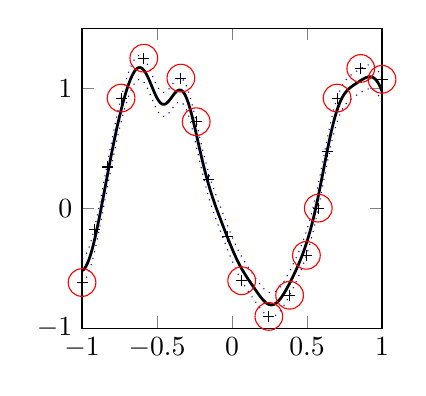
\begin{tikzpicture}

\begin{axis}[%
width=1.5in,
height=1.5in,
scale only axis,
xmin=-1,
xmax=1,
ymin=-1,
ymax=1.5,
]
\addplot [color=black,solid,line width=1.0pt,forget plot]
  table[row sep=crcr]{%
-1	-0.519478094668077\\
-0.993333333333333	-0.514825507574742\\
-0.986666666666667	-0.507262094265251\\
-0.98	-0.496773788492693\\
-0.973333333333333	-0.483374036442919\\
-0.966666666666667	-0.467102700679731\\
-0.96	-0.44802449180788\\
-0.953333333333333	-0.426226996583418\\
-0.946666666666667	-0.401818381592594\\
-0.94	-0.374924858241789\\
-0.933333333333333	-0.345687997429841\\
-0.926666666666667	-0.314261980903266\\
-0.92	-0.280810871133675\\
-0.913333333333333	-0.245505973018918\\
-0.906666666666667	-0.208523349390497\\
-0.9	-0.170041538950641\\
-0.893333333333333	-0.130239510707106\\
-0.886666666666667	-0.0892948741173161\\
-0.88	-0.0473823498889232\\
-0.873333333333333	-0.0046724935464809\\
-0.866666666666667	0.0386693468097557\\
-0.86	0.0824838650853762\\
-0.853333333333333	0.12661845549901\\
-0.846666666666667	0.170927727583658\\
-0.84	0.215273909227987\\
-0.833333333333333	0.259527164564083\\
-0.826666666666667	0.303565846549517\\
-0.82	0.347276695387817\\
-0.813333333333333	0.390554984291195\\
-0.806666666666667	0.433304604402104\\
-0.8	0.475438071866985\\
-0.793333333333333	0.516876432966788\\
-0.786666666666667	0.557549038621734\\
-0.78	0.597393158110438\\
-0.773333333333333	0.636353403876038\\
-0.766666666666667	0.674380944990661\\
-0.76	0.711432496105813\\
-0.753333333333333	0.747469081151547\\
-0.746666666666667	0.782454586026612\\
-0.74	0.816354131184007\\
-0.733333333333333	0.849132312320434\\
-0.726666666666667	0.88075137416338\\
-0.72	0.911169397405715\\
-0.713333333333333	0.94033859098118\\
-0.706666666666667	0.968203790025453\\
-0.7	0.994701263125414\\
-0.693333333333333	1.01975793016568\\
-0.686666666666667	1.04329108387454\\
-0.68	1.06520869402101\\
-0.673333333333333	1.08541035343889\\
-0.666666666666667	1.10378890031529\\
-0.66	1.12023272246109\\
-0.653333333333333	1.13462871783435\\
-0.646666666666667	1.14686585288109\\
-0.64	1.15683922789175\\
-0.633333333333333	1.16445452819591\\
-0.626666666666667	1.16963271324102\\
-0.62	1.17231477390253\\
-0.613333333333333	1.17246637301973\\
-0.606666666666667	1.17008217612957\\
-0.6	1.16518967932675\\
-0.593333333333333	1.15785234938695\\
-0.586666666666667	1.14817190763488\\
-0.58	1.13628961302065\\
-0.573333333333333	1.12238643062681\\
-0.566666666666667	1.10668200819173\\
-0.56	1.08943242377215\\
-0.553333333333333	1.07092671076492\\
-0.546666666666667	1.0514822104433\\
-0.54	1.03143884518773\\
-0.533333333333333	1.0111524460085\\
-0.526666666666667	0.990987304195452\\
-0.52	0.971308147603792\\
-0.513333333333333	0.952471766050984\\
-0.506666666666667	0.934818526691282\\
-0.5	0.918664028488233\\
-0.493333333333333	0.904291144770123\\
-0.486666666666667	0.891942694387121\\
-0.48	0.8818149655445\\
-0.473333333333333	0.874052292586399\\
-0.466666666666667	0.868742855708956\\
-0.46	0.865915837849192\\
-0.453333333333333	0.865540033042672\\
-0.446666666666667	0.867523957697591\\
-0.44	0.871717471892851\\
-0.433333333333333	0.877914873394389\\
-0.426666666666667	0.885859384000753\\
-0.42	0.895248907419515\\
-0.413333333333333	0.905742901386963\\
-0.406666666666667	0.916970175288169\\
-0.4	0.928537399061029\\
-0.393333333333333	0.940038090431452\\
-0.386666666666667	0.951061836065378\\
-0.38	0.961203498339904\\
-0.373333333333333	0.970072163186622\\
-0.366666666666667	0.977299595650559\\
-0.36	0.982547987995267\\
-0.353333333333333	0.985516809691437\\
-0.346666666666667	0.985948598561891\\
-0.34	0.983633566646007\\
-0.333333333333333	0.978412931772933\\
-0.326666666666667	0.97018092507787\\
-0.32	0.958885464393412\\
-0.313333333333333	0.944527522238603\\
-0.306666666666667	0.927159253712247\\
-0.3	0.906880982787093\\
-0.293333333333333	0.883837174270839\\
-0.286666666666667	0.858211542221693\\
-0.28	0.830221463284399\\
-0.273333333333333	0.800111874900607\\
-0.266666666666667	0.76814884355565\\
-0.26	0.734612987312948\\
-0.253333333333333	0.699792930251523\\
-0.246666666666667	0.663978954659455\\
-0.24	0.627457000710937\\
-0.233333333333333	0.590503143752884\\
-0.226666666666667	0.553378657208214\\
-0.22	0.516325745449658\\
-0.213333333333333	0.479564006769197\\
-0.206666666666667	0.443287662655236\\
-0.2	0.407663566779669\\
-0.193333333333333	0.372829986045469\\
-0.186666666666667	0.338896127256662\\
-0.18	0.30594236679228\\
-0.173333333333333	0.274021127281851\\
-0.166666666666667	0.243158334733012\\
-0.16	0.213355381763914\\
-0.153333333333333	0.184591517351692\\
-0.146666666666667	0.156826580554573\\
-0.14	0.130003994684364\\
-0.133333333333333	0.104053939066646\\
-0.126666666666667	0.0788966175079007\\
-0.12	0.0544455456059252\\
-0.113333333333333	0.0306107828586425\\
-0.106666666666667	0.00730203997693778\\
-0.1	-0.0155684032123372\\
-0.0933333333333333	-0.0380830284118963\\
-0.0866666666666666	-0.0603167111951857\\
-0.08	-0.0823347016170069\\
-0.0733333333333333	-0.104190992422378\\
-0.0666666666666667	-0.125927106171843\\
-0.0599999999999999	-0.147571323750008\\
-0.0533333333333332	-0.169138366996416\\
-0.0466666666666666	-0.190629537617701\\
-0.0399999999999999	-0.212033303205099\\
-0.0333333333333333	-0.233326309273542\\
-0.0266666666666666	-0.254474784026777\\
-0.0199999999999999	-0.275436290389981\\
-0.0133333333333333	-0.296161768163145\\
-0.0066666666666666	-0.316597798416668\\
1.11022302462516e-16	-0.336689012988835\\
0.00666666666666682	-0.356380564670765\\
0.0133333333333335	-0.37562056886769\\
0.0200000000000001	-0.394362425634874\\
0.0266666666666668	-0.412566932337916\\
0.0333333333333335	-0.43020410199355\\
0.0400000000000001	-0.447254610674344\\
0.0466666666666669	-0.463710809109887\\
0.0533333333333335	-0.479577248515177\\
0.0600000000000002	-0.494870688277101\\
0.0666666666666669	-0.50961957282215\\
0.0733333333333335	-0.523862986020261\\
0.0800000000000002	-0.537649112986104\\
0.0866666666666668	-0.551033260181912\\
0.0933333333333335	-0.564075504338108\\
0.1	-0.57683805794353\\
0.106666666666667	-0.589382453041292\\
0.113333333333334	-0.601766655045772\\
0.12	-0.614042223682689\\
0.126666666666667	-0.626251638563514\\
0.133333333333334	-0.63842590218416\\
0.14	-0.650582523380542\\
0.146666666666667	-0.662723969824937\\
0.153333333333334	-0.674836659591712\\
0.16	-0.686890539958641\\
0.166666666666667	-0.698839277418844\\
0.173333333333333	-0.710621057466641\\
0.18	-0.722159967270987\\
0.186666666666667	-0.733367910058109\\
0.193333333333333	-0.744146978035601\\
0.2	-0.754392192037305\\
0.206666666666667	-0.763994501618336\\
0.213333333333333	-0.772843929735327\\
0.22	-0.780832741812112\\
0.226666666666667	-0.787858520049519\\
0.233333333333334	-0.793827030147799\\
0.24	-0.79865477876357\\
0.246666666666667	-0.802271175371397\\
0.253333333333334	-0.804620230892196\\
0.26	-0.805661746483169\\
0.266666666666667	-0.805371968159174\\
0.273333333333334	-0.803743705303894\\
0.28	-0.800785932533307\\
0.286666666666667	-0.796522913788245\\
0.293333333333334	-0.790992904097646\\
0.3	-0.784246497499239\\
0.306666666666667	-0.776344698680521\\
0.313333333333333	-0.767356800798843\\
0.32	-0.757358152684601\\
0.326666666666667	-0.746427895484158\\
0.333333333333333	-0.73464674222067\\
0.34	-0.722094864369505\\
0.346666666666667	-0.708849938110029\\
0.353333333333333	-0.694985390246883\\
0.36	-0.680568870728866\\
0.366666666666667	-0.665660966035102\\
0.373333333333334	-0.650314156167704\\
0.38	-0.634572008187398\\
0.386666666666667	-0.618468591601073\\
0.393333333333334	-0.602028095733454\\
0.4	-0.585264626584119\\
0.406666666666667	-0.568182160504194\\
0.413333333333334	-0.550774634079151\\
0.42	-0.533026153490408\\
0.426666666666667	-0.514911311854692\\
0.433333333333334	-0.496395609038609\\
0.44	-0.477435974613652\\
0.446666666666667	-0.457981400354884\\
0.453333333333333	-0.437973693436389\\
0.46	-0.41734836475391\\
0.466666666666667	-0.396035668227456\\
0.473333333333333	-0.373961806244625\\
0.48	-0.351050313476832\\
0.486666666666667	-0.327223626156935\\
0.493333333333334	-0.302404836711895\\
0.5	-0.276519624696457\\
0.506666666666667	-0.249498344691474\\
0.513333333333334	-0.221278240731125\\
0.52	-0.191805745499527\\
0.526666666666667	-0.161038811628112\\
0.533333333333334	-0.128949212585845\\
0.54	-0.0955247425240781\\
0.546666666666667	-0.0607712386079747\\
0.553333333333333	-0.0247143463500237\\
0.56	0.0125990513358689\\
0.566666666666667	0.0510998169448625\\
0.573333333333333	0.0906960213297685\\
0.58	0.131272944179338\\
0.586666666666667	0.172693655185291\\
0.593333333333333	0.214800201868154\\
0.6	0.257415410447664\\
0.606666666666667	0.300345284875012\\
0.613333333333334	0.34338196702762\\
0.62	0.386307199030501\\
0.626666666666667	0.428896207691445\\
0.633333333333334	0.470921912106654\\
0.64	0.512159339552569\\
0.646666666666667	0.552390122679563\\
0.653333333333334	0.591406943473821\\
0.66	0.629017786979937\\
0.666666666666667	0.665049870681707\\
0.673333333333334	0.69935312377759\\
0.68	0.731803104152811\\
0.686666666666667	0.762303259172008\\
0.693333333333334	0.790786458776182\\
0.7	0.817215754827647\\
0.706666666666667	0.841584348092912\\
0.713333333333334	0.863914772450805\\
0.72	0.884257333569713\\
0.726666666666667	0.902687865133765\\
0.733333333333334	0.919304888517337\\
0.74	0.934226280566196\\
0.746666666666667	0.947585568010347\\
0.753333333333334	0.959527975438559\\
0.76	0.970206356434441\\
0.766666666666667	0.979777134448876\\
0.773333333333334	0.988396371614879\\
0.78	0.996216070639469\\
0.786666666666667	1.00338079802393\\
0.793333333333334	1.01002469725387\\
0.8	1.01626893947473\\
0.806666666666667	1.02221963778673\\
0.813333333333334	1.02796623088548\\
0.82	1.03358032346127\\
0.826666666666667	1.03911495549464\\
0.833333333333333	1.04460426105335\\
0.84	1.05006346983408\\
0.846666666666667	1.05548920162571\\
0.853333333333333	1.06086000492194\\
0.86	1.0661370956154\\
0.866666666666667	1.07126525935204\\
0.873333333333334	1.07617389081144\\
0.88	1.08077815387846\\
0.886666666666667	1.08498025731003\\
0.893333333333334	1.08867085003511\\
0.9	1.09173054771923\\
0.906666666666667	1.09403160691782\\
0.913333333333334	1.09543976450411\\
0.92	1.09581625782508\\
0.926666666666667	1.09502003523908\\
0.933333333333334	1.09291015763019\\
0.94	1.08934837975161\\
0.946666666666667	1.08420188661785\\
0.953333333333334	1.07734614560593\\
0.96	1.0686678204974\\
0.966666666666667	1.05806768048134\\
0.973333333333334	1.04546342617451\\
0.98	1.03079234690829\\
0.986666666666667	1.01401371960773\\
0.993333333333334	0.995110860033359\\
1	0.974092742194648\\
};
\addplot [color=blue,dotted,forget plot]
  table[row sep=crcr]{%
-1	-0.419478094668077\\
-0.993333333333333	-0.414825507574742\\
-0.986666666666667	-0.407262094265251\\
-0.98	-0.396773788492693\\
-0.973333333333333	-0.383374036442919\\
-0.966666666666667	-0.367102700679731\\
-0.96	-0.34802449180788\\
-0.953333333333333	-0.326226996583418\\
-0.946666666666667	-0.301818381592594\\
-0.94	-0.274924858241789\\
-0.933333333333333	-0.245687997429841\\
-0.926666666666667	-0.214261980903266\\
-0.92	-0.180810871133675\\
-0.913333333333333	-0.145505973018918\\
-0.906666666666667	-0.108523349390497\\
-0.9	-0.0700415389506414\\
-0.893333333333333	-0.0302395107071056\\
-0.886666666666667	0.0107051258826839\\
-0.88	0.0526176501110768\\
-0.873333333333333	0.0953275064535191\\
-0.866666666666667	0.138669346809756\\
-0.86	0.182483865085376\\
-0.853333333333333	0.22661845549901\\
-0.846666666666667	0.270927727583658\\
-0.84	0.315273909227987\\
-0.833333333333333	0.359527164564083\\
-0.826666666666667	0.403565846549517\\
-0.82	0.447276695387817\\
-0.813333333333333	0.490554984291195\\
-0.806666666666667	0.533304604402104\\
-0.8	0.575438071866985\\
-0.793333333333333	0.616876432966788\\
-0.786666666666667	0.657549038621734\\
-0.78	0.697393158110438\\
-0.773333333333333	0.736353403876038\\
-0.766666666666667	0.774380944990661\\
-0.76	0.811432496105813\\
-0.753333333333333	0.847469081151547\\
-0.746666666666667	0.882454586026612\\
-0.74	0.916354131184007\\
-0.733333333333333	0.949132312320434\\
-0.726666666666667	0.98075137416338\\
-0.72	1.01116939740571\\
-0.713333333333333	1.04033859098118\\
-0.706666666666667	1.06820379002545\\
-0.7	1.09470126312541\\
-0.693333333333333	1.11975793016568\\
-0.686666666666667	1.14329108387454\\
-0.68	1.16520869402101\\
-0.673333333333333	1.18541035343889\\
-0.666666666666667	1.20378890031529\\
-0.66	1.22023272246109\\
-0.653333333333333	1.23462871783435\\
-0.646666666666667	1.24686585288109\\
-0.64	1.25683922789175\\
-0.633333333333333	1.26445452819591\\
-0.626666666666667	1.26963271324102\\
-0.62	1.27231477390253\\
-0.613333333333333	1.27246637301973\\
-0.606666666666667	1.27008217612957\\
-0.6	1.26518967932675\\
-0.593333333333333	1.25785234938695\\
-0.586666666666667	1.24817190763488\\
-0.58	1.23628961302065\\
-0.573333333333333	1.22238643062681\\
-0.566666666666667	1.20668200819173\\
-0.56	1.18943242377215\\
-0.553333333333333	1.17092671076492\\
-0.546666666666667	1.1514822104433\\
-0.54	1.13143884518773\\
-0.533333333333333	1.1111524460085\\
-0.526666666666667	1.09098730419545\\
-0.52	1.07130814760379\\
-0.513333333333333	1.05247176605098\\
-0.506666666666667	1.03481852669128\\
-0.5	1.01866402848823\\
-0.493333333333333	1.00429114477012\\
-0.486666666666667	0.991942694387121\\
-0.48	0.9818149655445\\
-0.473333333333333	0.974052292586399\\
-0.466666666666667	0.968742855708956\\
-0.46	0.965915837849192\\
-0.453333333333333	0.965540033042672\\
-0.446666666666667	0.967523957697591\\
-0.44	0.971717471892851\\
-0.433333333333333	0.977914873394389\\
-0.426666666666667	0.985859384000753\\
-0.42	0.995248907419515\\
-0.413333333333333	1.00574290138696\\
-0.406666666666667	1.01697017528817\\
-0.4	1.02853739906103\\
-0.393333333333333	1.04003809043145\\
-0.386666666666667	1.05106183606538\\
-0.38	1.0612034983399\\
-0.373333333333333	1.07007216318662\\
-0.366666666666667	1.07729959565056\\
-0.36	1.08254798799527\\
-0.353333333333333	1.08551680969144\\
-0.346666666666667	1.08594859856189\\
-0.34	1.08363356664601\\
-0.333333333333333	1.07841293177293\\
-0.326666666666667	1.07018092507787\\
-0.32	1.05888546439341\\
-0.313333333333333	1.0445275222386\\
-0.306666666666667	1.02715925371225\\
-0.3	1.00688098278709\\
-0.293333333333333	0.983837174270839\\
-0.286666666666667	0.958211542221693\\
-0.28	0.930221463284399\\
-0.273333333333333	0.900111874900607\\
-0.266666666666667	0.86814884355565\\
-0.26	0.834612987312948\\
-0.253333333333333	0.799792930251523\\
-0.246666666666667	0.763978954659455\\
-0.24	0.727457000710937\\
-0.233333333333333	0.690503143752884\\
-0.226666666666667	0.653378657208214\\
-0.22	0.616325745449658\\
-0.213333333333333	0.579564006769197\\
-0.206666666666667	0.543287662655236\\
-0.2	0.507663566779669\\
-0.193333333333333	0.472829986045469\\
-0.186666666666667	0.438896127256662\\
-0.18	0.40594236679228\\
-0.173333333333333	0.374021127281851\\
-0.166666666666667	0.343158334733012\\
-0.16	0.313355381763914\\
-0.153333333333333	0.284591517351692\\
-0.146666666666667	0.256826580554573\\
-0.14	0.230003994684364\\
-0.133333333333333	0.204053939066646\\
-0.126666666666667	0.178896617507901\\
-0.12	0.154445545605925\\
-0.113333333333333	0.130610782858643\\
-0.106666666666667	0.107302039976938\\
-0.1	0.0844315967876628\\
-0.0933333333333333	0.0619169715881037\\
-0.0866666666666666	0.0396832888048143\\
-0.08	0.0176652983829931\\
-0.0733333333333333	-0.00419099242237794\\
-0.0666666666666667	-0.0259271061718427\\
-0.0599999999999999	-0.0475713237500079\\
-0.0533333333333332	-0.0691383669964158\\
-0.0466666666666666	-0.0906295376177006\\
-0.0399999999999999	-0.112033303205099\\
-0.0333333333333333	-0.133326309273542\\
-0.0266666666666666	-0.154474784026777\\
-0.0199999999999999	-0.175436290389981\\
-0.0133333333333333	-0.196161768163145\\
-0.0066666666666666	-0.216597798416668\\
1.11022302462516e-16	-0.236689012988835\\
0.00666666666666682	-0.256380564670765\\
0.0133333333333335	-0.27562056886769\\
0.0200000000000001	-0.294362425634874\\
0.0266666666666668	-0.312566932337916\\
0.0333333333333335	-0.33020410199355\\
0.0400000000000001	-0.347254610674344\\
0.0466666666666669	-0.363710809109887\\
0.0533333333333335	-0.379577248515177\\
0.0600000000000002	-0.394870688277101\\
0.0666666666666669	-0.40961957282215\\
0.0733333333333335	-0.423862986020261\\
0.0800000000000002	-0.437649112986104\\
0.0866666666666668	-0.451033260181912\\
0.0933333333333335	-0.464075504338108\\
0.1	-0.47683805794353\\
0.106666666666667	-0.489382453041292\\
0.113333333333334	-0.501766655045772\\
0.12	-0.514042223682689\\
0.126666666666667	-0.526251638563514\\
0.133333333333334	-0.53842590218416\\
0.14	-0.550582523380542\\
0.146666666666667	-0.562723969824937\\
0.153333333333334	-0.574836659591712\\
0.16	-0.586890539958641\\
0.166666666666667	-0.598839277418844\\
0.173333333333333	-0.610621057466641\\
0.18	-0.622159967270987\\
0.186666666666667	-0.633367910058109\\
0.193333333333333	-0.644146978035601\\
0.2	-0.654392192037305\\
0.206666666666667	-0.663994501618336\\
0.213333333333333	-0.672843929735327\\
0.22	-0.680832741812112\\
0.226666666666667	-0.687858520049519\\
0.233333333333334	-0.693827030147799\\
0.24	-0.69865477876357\\
0.246666666666667	-0.702271175371397\\
0.253333333333334	-0.704620230892196\\
0.26	-0.705661746483169\\
0.266666666666667	-0.705371968159174\\
0.273333333333334	-0.703743705303894\\
0.28	-0.700785932533307\\
0.286666666666667	-0.696522913788245\\
0.293333333333334	-0.690992904097646\\
0.3	-0.684246497499239\\
0.306666666666667	-0.676344698680521\\
0.313333333333333	-0.667356800798844\\
0.32	-0.657358152684601\\
0.326666666666667	-0.646427895484158\\
0.333333333333333	-0.63464674222067\\
0.34	-0.622094864369505\\
0.346666666666667	-0.608849938110029\\
0.353333333333333	-0.594985390246883\\
0.36	-0.580568870728866\\
0.366666666666667	-0.565660966035102\\
0.373333333333334	-0.550314156167704\\
0.38	-0.534572008187398\\
0.386666666666667	-0.518468591601073\\
0.393333333333334	-0.502028095733454\\
0.4	-0.485264626584119\\
0.406666666666667	-0.468182160504194\\
0.413333333333334	-0.450774634079151\\
0.42	-0.433026153490408\\
0.426666666666667	-0.414911311854692\\
0.433333333333334	-0.396395609038609\\
0.44	-0.377435974613652\\
0.446666666666667	-0.357981400354884\\
0.453333333333333	-0.337973693436389\\
0.46	-0.31734836475391\\
0.466666666666667	-0.296035668227456\\
0.473333333333333	-0.273961806244625\\
0.48	-0.251050313476832\\
0.486666666666667	-0.227223626156935\\
0.493333333333334	-0.202404836711895\\
0.5	-0.176519624696457\\
0.506666666666667	-0.149498344691474\\
0.513333333333334	-0.121278240731125\\
0.52	-0.0918057454995274\\
0.526666666666667	-0.0610388116281118\\
0.533333333333334	-0.0289492125858445\\
0.54	0.00447525747592188\\
0.546666666666667	0.0392287613920253\\
0.553333333333333	0.0752856536499763\\
0.56	0.112599051335869\\
0.566666666666667	0.151099816944862\\
0.573333333333333	0.190696021329769\\
0.58	0.231272944179338\\
0.586666666666667	0.272693655185291\\
0.593333333333333	0.314800201868154\\
0.6	0.357415410447664\\
0.606666666666667	0.400345284875012\\
0.613333333333334	0.44338196702762\\
0.62	0.486307199030501\\
0.626666666666667	0.528896207691445\\
0.633333333333334	0.570921912106654\\
0.64	0.612159339552569\\
0.646666666666667	0.652390122679563\\
0.653333333333334	0.691406943473821\\
0.66	0.729017786979937\\
0.666666666666667	0.765049870681707\\
0.673333333333334	0.79935312377759\\
0.68	0.831803104152811\\
0.686666666666667	0.862303259172008\\
0.693333333333334	0.890786458776182\\
0.7	0.917215754827647\\
0.706666666666667	0.941584348092912\\
0.713333333333334	0.963914772450805\\
0.72	0.984257333569713\\
0.726666666666667	1.00268786513377\\
0.733333333333334	1.01930488851734\\
0.74	1.0342262805662\\
0.746666666666667	1.04758556801035\\
0.753333333333334	1.05952797543856\\
0.76	1.07020635643444\\
0.766666666666667	1.07977713444888\\
0.773333333333334	1.08839637161488\\
0.78	1.09621607063947\\
0.786666666666667	1.10338079802393\\
0.793333333333334	1.11002469725387\\
0.8	1.11626893947473\\
0.806666666666667	1.12221963778673\\
0.813333333333334	1.12796623088548\\
0.82	1.13358032346127\\
0.826666666666667	1.13911495549464\\
0.833333333333333	1.14460426105335\\
0.84	1.15006346983408\\
0.846666666666667	1.15548920162571\\
0.853333333333333	1.16086000492194\\
0.86	1.1661370956154\\
0.866666666666667	1.17126525935204\\
0.873333333333334	1.17617389081144\\
0.88	1.18077815387846\\
0.886666666666667	1.18498025731003\\
0.893333333333334	1.18867085003511\\
0.9	1.19173054771923\\
0.906666666666667	1.19403160691782\\
0.913333333333334	1.19543976450411\\
0.92	1.19581625782508\\
0.926666666666667	1.19502003523908\\
0.933333333333334	1.19291015763019\\
0.94	1.18934837975161\\
0.946666666666667	1.18420188661785\\
0.953333333333334	1.17734614560593\\
0.96	1.1686678204974\\
0.966666666666667	1.15806768048134\\
0.973333333333334	1.14546342617451\\
0.98	1.13079234690829\\
0.986666666666667	1.11401371960773\\
0.993333333333334	1.09511086003336\\
1	1.07409274219465\\
};
\addplot [color=blue,dotted,forget plot]
  table[row sep=crcr]{%
-1	-0.619478094668077\\
-0.993333333333333	-0.614825507574742\\
-0.986666666666667	-0.607262094265251\\
-0.98	-0.596773788492693\\
-0.973333333333333	-0.583374036442919\\
-0.966666666666667	-0.567102700679731\\
-0.96	-0.54802449180788\\
-0.953333333333333	-0.526226996583418\\
-0.946666666666667	-0.501818381592594\\
-0.94	-0.474924858241789\\
-0.933333333333333	-0.445687997429841\\
-0.926666666666667	-0.414261980903266\\
-0.92	-0.380810871133675\\
-0.913333333333333	-0.345505973018918\\
-0.906666666666667	-0.308523349390497\\
-0.9	-0.270041538950641\\
-0.893333333333333	-0.230239510707106\\
-0.886666666666667	-0.189294874117316\\
-0.88	-0.147382349888923\\
-0.873333333333333	-0.104672493546481\\
-0.866666666666667	-0.0613306531902443\\
-0.86	-0.0175161349146238\\
-0.853333333333333	0.0266184554990097\\
-0.846666666666667	0.0709277275836581\\
-0.84	0.115273909227987\\
-0.833333333333333	0.159527164564083\\
-0.826666666666667	0.203565846549517\\
-0.82	0.247276695387817\\
-0.813333333333333	0.290554984291195\\
-0.806666666666667	0.333304604402104\\
-0.8	0.375438071866985\\
-0.793333333333333	0.416876432966788\\
-0.786666666666667	0.457549038621734\\
-0.78	0.497393158110438\\
-0.773333333333333	0.536353403876038\\
-0.766666666666667	0.574380944990661\\
-0.76	0.611432496105813\\
-0.753333333333333	0.647469081151547\\
-0.746666666666667	0.682454586026612\\
-0.74	0.716354131184007\\
-0.733333333333333	0.749132312320434\\
-0.726666666666667	0.78075137416338\\
-0.72	0.811169397405715\\
-0.713333333333333	0.84033859098118\\
-0.706666666666667	0.868203790025453\\
-0.7	0.894701263125414\\
-0.693333333333333	0.919757930165678\\
-0.686666666666667	0.943291083874541\\
-0.68	0.965208694021012\\
-0.673333333333333	0.985410353438887\\
-0.666666666666667	1.00378890031529\\
-0.66	1.02023272246109\\
-0.653333333333333	1.03462871783435\\
-0.646666666666667	1.04686585288109\\
-0.64	1.05683922789175\\
-0.633333333333333	1.06445452819591\\
-0.626666666666667	1.06963271324102\\
-0.62	1.07231477390253\\
-0.613333333333333	1.07246637301973\\
-0.606666666666667	1.07008217612957\\
-0.6	1.06518967932675\\
-0.593333333333333	1.05785234938695\\
-0.586666666666667	1.04817190763488\\
-0.58	1.03628961302065\\
-0.573333333333333	1.02238643062681\\
-0.566666666666667	1.00668200819173\\
-0.56	0.98943242377215\\
-0.553333333333333	0.970926710764923\\
-0.546666666666667	0.951482210443305\\
-0.54	0.931438845187733\\
-0.533333333333333	0.911152446008501\\
-0.526666666666667	0.890987304195452\\
-0.52	0.871308147603792\\
-0.513333333333333	0.852471766050984\\
-0.506666666666667	0.834818526691282\\
-0.5	0.818664028488233\\
-0.493333333333333	0.804291144770123\\
-0.486666666666667	0.791942694387121\\
-0.48	0.7818149655445\\
-0.473333333333333	0.774052292586399\\
-0.466666666666667	0.768742855708956\\
-0.46	0.765915837849192\\
-0.453333333333333	0.765540033042672\\
-0.446666666666667	0.767523957697591\\
-0.44	0.771717471892851\\
-0.433333333333333	0.777914873394389\\
-0.426666666666667	0.785859384000754\\
-0.42	0.795248907419515\\
-0.413333333333333	0.805742901386963\\
-0.406666666666667	0.816970175288169\\
-0.4	0.828537399061029\\
-0.393333333333333	0.840038090431452\\
-0.386666666666667	0.851061836065378\\
-0.38	0.861203498339904\\
-0.373333333333333	0.870072163186622\\
-0.366666666666667	0.877299595650559\\
-0.36	0.882547987995267\\
-0.353333333333333	0.885516809691437\\
-0.346666666666667	0.885948598561891\\
-0.34	0.883633566646007\\
-0.333333333333333	0.878412931772933\\
-0.326666666666667	0.87018092507787\\
-0.32	0.858885464393412\\
-0.313333333333333	0.844527522238603\\
-0.306666666666667	0.827159253712247\\
-0.3	0.806880982787093\\
-0.293333333333333	0.783837174270839\\
-0.286666666666667	0.758211542221693\\
-0.28	0.730221463284399\\
-0.273333333333333	0.700111874900607\\
-0.266666666666667	0.66814884355565\\
-0.26	0.634612987312948\\
-0.253333333333333	0.599792930251523\\
-0.246666666666667	0.563978954659455\\
-0.24	0.527457000710937\\
-0.233333333333333	0.490503143752884\\
-0.226666666666667	0.453378657208214\\
-0.22	0.416325745449658\\
-0.213333333333333	0.379564006769197\\
-0.206666666666667	0.343287662655236\\
-0.2	0.307663566779669\\
-0.193333333333333	0.272829986045469\\
-0.186666666666667	0.238896127256662\\
-0.18	0.20594236679228\\
-0.173333333333333	0.174021127281851\\
-0.166666666666667	0.143158334733012\\
-0.16	0.113355381763914\\
-0.153333333333333	0.0845915173516917\\
-0.146666666666667	0.0568265805545735\\
-0.14	0.0300039946843644\\
-0.133333333333333	0.00405393906664567\\
-0.126666666666667	-0.0211033824920993\\
-0.12	-0.0455544543940748\\
-0.113333333333333	-0.0693892171413575\\
-0.106666666666667	-0.0926979600230622\\
-0.1	-0.115568403212337\\
-0.0933333333333333	-0.138083028411896\\
-0.0866666666666666	-0.160316711195186\\
-0.08	-0.182334701617007\\
-0.0733333333333333	-0.204190992422378\\
-0.0666666666666667	-0.225927106171843\\
-0.0599999999999999	-0.247571323750008\\
-0.0533333333333332	-0.269138366996416\\
-0.0466666666666666	-0.290629537617701\\
-0.0399999999999999	-0.312033303205099\\
-0.0333333333333333	-0.333326309273542\\
-0.0266666666666666	-0.354474784026777\\
-0.0199999999999999	-0.375436290389981\\
-0.0133333333333333	-0.396161768163145\\
-0.0066666666666666	-0.416597798416668\\
1.11022302462516e-16	-0.436689012988835\\
0.00666666666666682	-0.456380564670765\\
0.0133333333333335	-0.47562056886769\\
0.0200000000000001	-0.494362425634874\\
0.0266666666666668	-0.512566932337916\\
0.0333333333333335	-0.530204101993551\\
0.0400000000000001	-0.547254610674344\\
0.0466666666666669	-0.563710809109887\\
0.0533333333333335	-0.579577248515177\\
0.0600000000000002	-0.594870688277101\\
0.0666666666666669	-0.60961957282215\\
0.0733333333333335	-0.623862986020261\\
0.0800000000000002	-0.637649112986104\\
0.0866666666666668	-0.651033260181912\\
0.0933333333333335	-0.664075504338108\\
0.1	-0.67683805794353\\
0.106666666666667	-0.689382453041292\\
0.113333333333334	-0.701766655045772\\
0.12	-0.714042223682689\\
0.126666666666667	-0.726251638563514\\
0.133333333333334	-0.73842590218416\\
0.14	-0.750582523380542\\
0.146666666666667	-0.762723969824937\\
0.153333333333334	-0.774836659591712\\
0.16	-0.786890539958641\\
0.166666666666667	-0.798839277418844\\
0.173333333333333	-0.810621057466641\\
0.18	-0.822159967270987\\
0.186666666666667	-0.833367910058109\\
0.193333333333333	-0.844146978035601\\
0.2	-0.854392192037305\\
0.206666666666667	-0.863994501618336\\
0.213333333333333	-0.872843929735327\\
0.22	-0.880832741812112\\
0.226666666666667	-0.887858520049518\\
0.233333333333334	-0.893827030147799\\
0.24	-0.89865477876357\\
0.246666666666667	-0.902271175371397\\
0.253333333333334	-0.904620230892196\\
0.26	-0.905661746483169\\
0.266666666666667	-0.905371968159174\\
0.273333333333334	-0.903743705303894\\
0.28	-0.900785932533307\\
0.286666666666667	-0.896522913788245\\
0.293333333333334	-0.890992904097646\\
0.3	-0.884246497499239\\
0.306666666666667	-0.876344698680521\\
0.313333333333333	-0.867356800798843\\
0.32	-0.857358152684601\\
0.326666666666667	-0.846427895484158\\
0.333333333333333	-0.83464674222067\\
0.34	-0.822094864369505\\
0.346666666666667	-0.808849938110029\\
0.353333333333333	-0.794985390246883\\
0.36	-0.780568870728866\\
0.366666666666667	-0.765660966035102\\
0.373333333333334	-0.750314156167704\\
0.38	-0.734572008187398\\
0.386666666666667	-0.718468591601073\\
0.393333333333334	-0.702028095733454\\
0.4	-0.685264626584119\\
0.406666666666667	-0.668182160504194\\
0.413333333333334	-0.650774634079151\\
0.42	-0.633026153490408\\
0.426666666666667	-0.614911311854692\\
0.433333333333334	-0.596395609038609\\
0.44	-0.577435974613652\\
0.446666666666667	-0.557981400354884\\
0.453333333333333	-0.537973693436389\\
0.46	-0.51734836475391\\
0.466666666666667	-0.496035668227456\\
0.473333333333333	-0.473961806244625\\
0.48	-0.451050313476832\\
0.486666666666667	-0.427223626156935\\
0.493333333333334	-0.402404836711895\\
0.5	-0.376519624696457\\
0.506666666666667	-0.349498344691474\\
0.513333333333334	-0.321278240731125\\
0.52	-0.291805745499527\\
0.526666666666667	-0.261038811628112\\
0.533333333333334	-0.228949212585845\\
0.54	-0.195524742524078\\
0.546666666666667	-0.160771238607975\\
0.553333333333333	-0.124714346350024\\
0.56	-0.0874009486641311\\
0.566666666666667	-0.0489001830551375\\
0.573333333333333	-0.0093039786702315\\
0.58	0.0312729441793378\\
0.586666666666667	0.0726936551852912\\
0.593333333333333	0.114800201868154\\
0.6	0.157415410447664\\
0.606666666666667	0.200345284875012\\
0.613333333333334	0.24338196702762\\
0.62	0.286307199030501\\
0.626666666666667	0.328896207691445\\
0.633333333333334	0.370921912106654\\
0.64	0.412159339552569\\
0.646666666666667	0.452390122679563\\
0.653333333333334	0.491406943473821\\
0.66	0.529017786979937\\
0.666666666666667	0.565049870681707\\
0.673333333333334	0.59935312377759\\
0.68	0.631803104152811\\
0.686666666666667	0.662303259172008\\
0.693333333333334	0.690786458776182\\
0.7	0.717215754827647\\
0.706666666666667	0.741584348092912\\
0.713333333333334	0.763914772450805\\
0.72	0.784257333569713\\
0.726666666666667	0.802687865133765\\
0.733333333333334	0.819304888517337\\
0.74	0.834226280566196\\
0.746666666666667	0.847585568010347\\
0.753333333333334	0.859527975438559\\
0.76	0.870206356434441\\
0.766666666666667	0.879777134448876\\
0.773333333333334	0.888396371614879\\
0.78	0.89621607063947\\
0.786666666666667	0.90338079802393\\
0.793333333333334	0.910024697253871\\
0.8	0.916268939474728\\
0.806666666666667	0.922219637786728\\
0.813333333333334	0.927966230885479\\
0.82	0.933580323461274\\
0.826666666666667	0.939114955494644\\
0.833333333333333	0.944604261053352\\
0.84	0.950063469834083\\
0.846666666666667	0.955489201625707\\
0.853333333333333	0.960860004921936\\
0.86	0.966137095615399\\
0.866666666666667	0.971265259352041\\
0.873333333333334	0.976173890811445\\
0.88	0.98077815387846\\
0.886666666666667	0.984980257310029\\
0.893333333333334	0.988670850035113\\
0.9	0.991730547719227\\
0.906666666666667	0.994031606917818\\
0.913333333333334	0.995439764504106\\
0.92	0.99581625782508\\
0.926666666666667	0.99502003523908\\
0.933333333333334	0.992910157630194\\
0.94	0.989348379751606\\
0.946666666666667	0.984201886617849\\
0.953333333333334	0.977346145605931\\
0.96	0.968667820497397\\
0.966666666666667	0.958067680481341\\
0.973333333333334	0.945463426174507\\
0.98	0.930792346908292\\
0.986666666666667	0.914013719607729\\
0.993333333333334	0.895110860033359\\
1	0.874092742194648\\
};
\addplot [color=black,only marks,mark=+,mark options={solid},forget plot]
  table[row sep=crcr]{%
-1	-0.61945564516129\\
};
\addplot [color=red,mark size=5.0pt,only marks,mark=o,mark options={solid},forget plot]
  table[row sep=crcr]{%
-1	-0.61945564516129\\
};
\addplot [color=black,only marks,mark=+,mark options={solid},forget plot]
  table[row sep=crcr]{%
-0.917627677100494	-0.175907258064516\\
};
\addplot [color=black,only marks,mark=+,mark options={solid},forget plot]
  table[row sep=crcr]{%
-0.828665568369028	0.343245967741936\\
};
\addplot [color=black,only marks,mark=+,mark options={solid},forget plot]
  table[row sep=crcr]{%
-0.739703459637562	0.917842741935484\\
};
\addplot [color=red,mark size=5.0pt,only marks,mark=o,mark options={solid},forget plot]
  table[row sep=crcr]{%
-0.739703459637562	0.917842741935484\\
};
\addplot [color=black,only marks,mark=+,mark options={solid},forget plot]
  table[row sep=crcr]{%
-0.588138385502471	1.25050403225806\\
};
\addplot [color=red,mark size=5.0pt,only marks,mark=o,mark options={solid},forget plot]
  table[row sep=crcr]{%
-0.588138385502471	1.25050403225806\\
};
\addplot [color=black,only marks,mark=+,mark options={solid},forget plot]
  table[row sep=crcr]{%
-0.341021416803954	1.08417338709677\\
};
\addplot [color=red,mark size=5.0pt,only marks,mark=o,mark options={solid},forget plot]
  table[row sep=crcr]{%
-0.341021416803954	1.08417338709677\\
};
\addplot [color=black,only marks,mark=+,mark options={solid},forget plot]
  table[row sep=crcr]{%
-0.238879736408567	0.721270161290323\\
};
\addplot [color=red,mark size=5.0pt,only marks,mark=o,mark options={solid},forget plot]
  table[row sep=crcr]{%
-0.238879736408567	0.721270161290323\\
};
\addplot [color=black,only marks,mark=+,mark options={solid},forget plot]
  table[row sep=crcr]{%
-0.156507413509061	0.237399193548388\\
};
\addplot [color=black,only marks,mark=+,mark options={solid},forget plot]
  table[row sep=crcr]{%
-0.0280065897858319	-0.236391129032258\\
};
\addplot [color=black,only marks,mark=+,mark options={solid},forget plot]
  table[row sep=crcr]{%
0.0642504118616145	-0.604334677419354\\
};
\addplot [color=red,mark size=5.0pt,only marks,mark=o,mark options={solid},forget plot]
  table[row sep=crcr]{%
0.0642504118616145	-0.604334677419354\\
};
\addplot [color=black,only marks,mark=+,mark options={solid},forget plot]
  table[row sep=crcr]{%
0.245469522240527	-0.901713709677419\\
};
\addplot [color=red,mark size=5.0pt,only marks,mark=o,mark options={solid},forget plot]
  table[row sep=crcr]{%
0.245469522240527	-0.901713709677419\\
};
\addplot [color=black,only marks,mark=+,mark options={solid},forget plot]
  table[row sep=crcr]{%
0.383855024711697	-0.725302419354838\\
};
\addplot [color=red,mark size=5.0pt,only marks,mark=o,mark options={solid},forget plot]
  table[row sep=crcr]{%
0.383855024711697	-0.725302419354838\\
};
\addplot [color=black,only marks,mark=+,mark options={solid},forget plot]
  table[row sep=crcr]{%
0.495881383855025	-0.392641129032258\\
};
\addplot [color=red,mark size=5.0pt,only marks,mark=o,mark options={solid},forget plot]
  table[row sep=crcr]{%
0.495881383855025	-0.392641129032258\\
};
\addplot [color=black,only marks,mark=+,mark options={solid},forget plot]
  table[row sep=crcr]{%
0.574958813838551	0.000504032258065168\\
};
\addplot [color=red,mark size=5.0pt,only marks,mark=o,mark options={solid},forget plot]
  table[row sep=crcr]{%
0.574958813838551	0.000504032258065168\\
};
\addplot [color=black,only marks,mark=+,mark options={solid},forget plot]
  table[row sep=crcr]{%
0.634266886326194	0.469254032258065\\
};
\addplot [color=black,only marks,mark=+,mark options={solid},forget plot]
  table[row sep=crcr]{%
0.700164744645799	0.917842741935484\\
};
\addplot [color=red,mark size=5.0pt,only marks,mark=o,mark options={solid},forget plot]
  table[row sep=crcr]{%
0.700164744645799	0.917842741935484\\
};
\addplot [color=black,only marks,mark=+,mark options={solid},forget plot]
  table[row sep=crcr]{%
0.85831960461285	1.1648185483871\\
};
\addplot [color=red,mark size=5.0pt,only marks,mark=o,mark options={solid},forget plot]
  table[row sep=crcr]{%
0.85831960461285	1.1648185483871\\
};
\addplot [color=black,only marks,mark=+,mark options={solid},forget plot]
  table[row sep=crcr]{%
1	1.07409274193548\\
};
\addplot [color=red,mark size=5.0pt,only marks,mark=o,mark options={solid},forget plot]
  table[row sep=crcr]{%
1	1.07409274193548\\
};
\end{axis}
\end{tikzpicture}%
\end{document}
% This file was created by matlab2tikz.
% Minimal pgfplots version: 1.3
%
%The latest updates can be retrieved from
%  http://www.mathworks.com/matlabcentral/fileexchange/22022-matlab2tikz
%where you can also make suggestions and rate matlab2tikz.
%
\documentclass[tikz]{standalone}
\usepackage{pgfplots}
\usepackage{grffile}
\pgfplotsset{compat=newest}
\usetikzlibrary{plotmarks}
\usepackage{amsmath}

\begin{document}
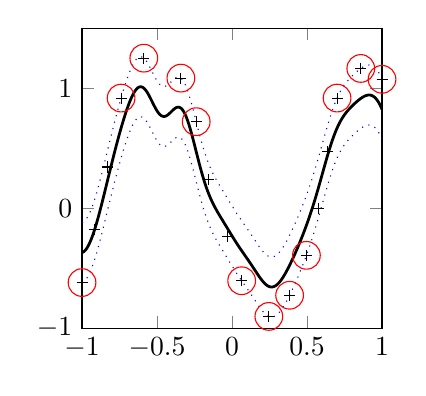
\begin{tikzpicture}

\begin{axis}[%
width=1.5in,
height=1.5in,
scale only axis,
xmin=-1,
xmax=1,
ymin=-1,
ymax=1.5,
]
\addplot [color=black,solid,line width=1.0pt,forget plot]
  table[row sep=crcr]{%
-1	-0.369455646991128\\
-0.993333333333333	-0.365916868887091\\
-0.986666666666667	-0.360266343254397\\
-0.98	-0.352489752410029\\
-0.973333333333333	-0.342592114305454\\
-0.966666666666667	-0.330597015339957\\
-0.96	-0.316545511363422\\
-0.953333333333333	-0.300494745649599\\
-0.946666666666667	-0.282516339807201\\
-0.94	-0.26269461808719\\
-0.933333333333333	-0.241124727195289\\
-0.926666666666667	-0.217910712539615\\
-0.92	-0.193163608000539\\
-0.913333333333333	-0.166999590116738\\
-0.906666666666667	-0.139538239479913\\
-0.9	-0.110900942665605\\
-0.893333333333333	-0.0812094578139336\\
-0.886666666666667	-0.0505846566592942\\
-0.88	-0.0191454460319063\\
-0.873333333333333	0.0129921367913413\\
-0.866666666666667	0.0457156675181953\\
-0.86	0.0789169346711418\\
-0.853333333333333	0.112492416153036\\
-0.846666666666667	0.146343653261192\\
-0.84	0.18037754098664\\
-0.833333333333333	0.214506549564685\\
-0.826666666666667	0.248648886788117\\
-0.82	0.282728604092392\\
-0.813333333333333	0.316675642502783\\
-0.806666666666667	0.350425807878081\\
-0.8	0.383920659179892\\
-0.793333333333333	0.417107289383629\\
-0.786666666666667	0.44993797667844\\
-0.78	0.482369684196\\
-0.773333333333333	0.514363389908993\\
-0.766666666666667	0.545883234599376\\
-0.76	0.576895484752555\\
-0.753333333333333	0.607367318512542\\
-0.746666666666667	0.637265455861439\\
-0.74	0.666554668217902\\
-0.733333333333333	0.695196216803771\\
-0.726666666666667	0.723146282442732\\
-0.72	0.750354460941233\\
-0.713333333333333	0.776762406908424\\
-0.706666666666667	0.80230271394709\\
-0.7	0.826898119899598\\
-0.693333333333333	0.850461121781538\\
-0.686666666666667	0.872894075953906\\
-0.68	0.894089845025592\\
-0.673333333333333	0.913933034286156\\
-0.666666666666667	0.932301837774219\\
-0.66	0.949070488280854\\
-0.653333333333333	0.964112277783129\\
-0.646666666666667	0.977303086280926\\
-0.64	0.988525329152485\\
-0.633333333333333	0.997672207361961\\
-0.626666666666667	1.00465212250947\\
-0.62	1.00939310105274\\
-0.613333333333333	1.01184706010154\\
-0.606666666666667	1.01199374179367\\
-0.6	1.00984414491347\\
-0.593333333333333	1.00544329129455\\
-0.586666666666667	0.998872180507151\\
-0.58	0.990248808887341\\
-0.573333333333333	0.979728157333298\\
-0.566666666666667	0.967501085419764\\
-0.56	0.953792105995657\\
-0.553333333333333	0.938856053107213\\
-0.546666666666667	0.922973695317668\\
-0.54	0.906446384743018\\
-0.533333333333333	0.889589867909146\\
-0.526666666666667	0.872727416486134\\
-0.52	0.856182462863697\\
-0.513333333333333	0.840270946398944\\
-0.506666666666667	0.825293590237865\\
-0.5	0.81152833539144\\
-0.493333333333333	0.799223158014341\\
-0.486666666666667	0.788589487636635\\
-0.48	0.779796428742335\\
-0.473333333333333	0.772965966115978\\
-0.466666666666667	0.768169306543109\\
-0.46	0.765424476685067\\
-0.453333333333333	0.764695260328823\\
-0.446666666666667	0.76589151892175\\
-0.44	0.768870898591188\\
-0.433333333333333	0.773441886002464\\
-0.426666666666667	0.779368135703839\\
-0.42	0.786373954277393\\
-0.413333333333333	0.794150792818768\\
-0.406666666666667	0.80236457005336\\
-0.4	0.810663624668186\\
-0.393333333333333	0.818687077934171\\
-0.386666666666667	0.826073376956041\\
-0.38	0.832468785245476\\
-0.373333333333333	0.837535590868356\\
-0.366666666666667	0.840959813033002\\
-0.36	0.842458205290835\\
-0.353333333333333	0.841784376912744\\
-0.346666666666667	0.838733882670808\\
-0.34	0.833148164197502\\
-0.333333333333333	0.824917262163055\\
-0.326666666666667	0.813981256447309\\
-0.32	0.800330429964389\\
-0.313333333333333	0.784004189496788\\
-0.306666666666667	0.765088812523892\\
-0.3	0.743714121399066\\
-0.293333333333333	0.720049214294634\\
-0.286666666666667	0.694297405238646\\
-0.28	0.666690542675461\\
-0.273333333333333	0.637482886902178\\
-0.266666666666667	0.606944731328784\\
-0.26	0.575355950899215\\
-0.253333333333333	0.542999653552084\\
-0.246666666666667	0.51015609786784\\
-0.24	0.477097022799074\\
-0.233333333333333	0.444080514506777\\
-0.226666666666667	0.411346511813126\\
-0.22	0.379113026657734\\
-0.213333333333333	0.347573130228364\\
-0.206666666666667	0.316892730093856\\
-0.2	0.287209139566922\\
-0.193333333333333	0.258630418410546\\
-0.186666666666667	0.231235444465565\\
-0.18	0.205074659244595\\
-0.173333333333333	0.180171417265326\\
-0.166666666666667	0.156523858976259\\
-0.16	0.13410722050201\\
-0.153333333333333	0.112876489915214\\
-0.146666666666667	0.0927693190366628\\
-0.14	0.0737091015088996\\
-0.133333333333333	0.0556081316720626\\
-0.126666666666667	0.0383707641709359\\
-0.12	0.0218965008286168\\
-0.113333333333333	0.00608293875994748\\
-0.106666666666667	-0.00917147835506454\\
-0.1	-0.0239649557191899\\
-0.0933333333333333	-0.0383901312076778\\
-0.0866666666666666	-0.0525321809178015\\
-0.08	-0.0664672718130549\\
-0.0733333333333333	-0.0802613788437899\\
-0.0666666666666667	-0.093969476080758\\
-0.0599999999999999	-0.107635103621248\\
-0.0533333333333332	-0.121290304281687\\
-0.0466666666666666	-0.134955916356869\\
-0.0399999999999999	-0.148642201019206\\
-0.0333333333333333	-0.162349775311614\\
-0.0266666666666666	-0.176070814267171\\
-0.0199999999999999	-0.189790478633963\\
-0.0133333333333333	-0.203488518211763\\
-0.0066666666666666	-0.21714099517731\\
1.11022302462516e-16	-0.230722067273828\\
0.00666666666666682	-0.244205767665052\\
0.0133333333333335	-0.25756771689014\\
0.0200000000000001	-0.270786702955746\\
0.0266666666666668	-0.28384606836076\\
0.0333333333333335	-0.296734847885613\\
0.0400000000000001	-0.30944860831328\\
0.0466666666666669	-0.321989950795084\\
0.0533333333333335	-0.334368648125421\\
0.0600000000000002	-0.346601402421134\\
0.0666666666666669	-0.358711223176598\\
0.0733333333333335	-0.370726440849085\\
0.0800000000000002	-0.382679386407061\\
0.0866666666666668	-0.394604781982371\\
0.0933333333333335	-0.406537901222665\\
0.1	-0.418512569476267\\
0.106666666666667	-0.430559082944915\\
0.113333333333334	-0.442702131886592\\
0.12	-0.454958815439704\\
0.126666666666667	-0.467336834420064\\
0.133333333333334	-0.479832943433581\\
0.14	-0.492431734953528\\
0.146666666666667	-0.505104815920746\\
0.153333333333334	-0.517810422404856\\
0.16	-0.530493500540563\\
0.166666666666667	-0.54308626308313\\
0.173333333333333	-0.555509211364055\\
0.18	-0.56767259307742\\
0.186666666666667	-0.579478248100559\\
0.193333333333333	-0.590821778318217\\
0.2	-0.601594963956027\\
0.206666666666667	-0.611688338883039\\
0.213333333333333	-0.620993831191501\\
0.22	-0.629407373386266\\
0.226666666666667	-0.636831388785271\\
0.233333333333334	-0.643177067098782\\
0.24	-0.648366352262378\\
0.246666666666667	-0.652333578902213\\
0.253333333333334	-0.655026709608258\\
0.26	-0.656408142661476\\
0.266666666666667	-0.656455078112181\\
0.273333333333334	-0.655159448225932\\
0.28	-0.652527435416733\\
0.286666666666667	-0.648578616069991\\
0.293333333333334	-0.643344781436244\\
0.3	-0.636868496524567\\
0.306666666666667	-0.629201464297882\\
0.313333333333333	-0.62040276532322\\
0.32	-0.61053704240901\\
0.326666666666667	-0.5996726959076\\
0.333333333333333	-0.587880148681057\\
0.34	-0.575230230765744\\
0.346666666666667	-0.561792723170179\\
0.353333333333333	-0.547635088702902\\
0.36	-0.532821405968366\\
0.366666666666667	-0.517411511375727\\
0.373333333333334	-0.501460343795992\\
0.38	-0.485017477893309\\
0.386666666666667	-0.468126825534055\\
0.393333333333334	-0.45082648028582\\
0.4	-0.433148677947711\\
0.406666666666667	-0.415119846243752\\
0.413333333333334	-0.396760719063093\\
0.42	-0.378086494624338\\
0.426666666666667	-0.359107022260896\\
0.433333333333334	-0.339827008687905\\
0.44	-0.320246241102503\\
0.446666666666667	-0.30035983076933\\
0.453333333333333	-0.280158486361953\\
0.46	-0.259628830834498\\
0.466666666666667	-0.238753778632455\\
0.473333333333333	-0.217512991361087\\
0.48	-0.195883429468821\\
0.486666666666667	-0.173840015041794\\
0.493333333333334	-0.151356416531541\\
0.5	-0.128405960348157\\
0.506666666666667	-0.10496266704324\\
0.513333333333334	-0.0810024016618745\\
0.52	-0.0565041192071555\\
0.526666666666667	-0.0314511775237598\\
0.533333333333334	-0.00583268177773459\\
0.54	0.0203551824084937\\
0.546666666666667	0.0471078757405399\\
0.553333333333333	0.0744113442604782\\
0.56	0.102241024367281\\
0.566666666666667	0.130561066627672\\
0.573333333333333	0.159323827518895\\
0.58	0.188469671970799\\
0.586666666666667	0.217927120785007\\
0.593333333333333	0.247613365957531\\
0.6	0.277435163999839\\
0.606666666666667	0.307290103039584\\
0.613333333333334	0.337068224382003\\
0.62	0.366653963996227\\
0.626666666666667	0.395928364771834\\
0.633333333333334	0.42477149709508\\
0.64	0.453065014019739\\
0.646666666666667	0.480694758689093\\
0.653333333333334	0.507553336236089\\
0.66	0.533542560546115\\
0.666666666666667	0.558575688245229\\
0.673333333333334	0.582579358125563\\
0.68	0.605495163791844\\
0.686666666666667	0.627280800264065\\
0.693333333333334	0.647910741069203\\
0.7	0.667376420302363\\
0.706666666666667	0.685685913404258\\
0.713333333333334	0.702863130066613\\
0.72	0.718946551777001\\
0.726666666666667	0.733987564099086\\
0.733333333333334	0.74804844897006\\
0.74	0.761200114320554\\
0.746666666666667	0.773519646587634\\
0.753333333333334	0.785087775807802\\
0.76	0.795986342785677\\
0.766666666666667	0.806295853420873\\
0.773333333333334	0.816093196968411\\
0.78	0.825449593358249\\
0.786666666666667	0.834428820450208\\
0.793333333333334	0.843085756140336\\
0.8	0.851465253542597\\
0.806666666666667	0.859601351052836\\
0.813333333333334	0.867516803931313\\
0.82	0.875222910987471\\
0.826666666666667	0.882719599732721\\
0.833333333333333	0.88999572649837\\
0.84	0.897029544776192\\
0.846666666666667	0.903789295456215\\
0.853333333333333	0.910233876485411\\
0.86	0.916313556292647\\
0.866666666666667	0.921970704458163\\
0.873333333333334	0.927140523734425\\
0.88	0.931751778737475\\
0.886666666666667	0.935727527480216\\
0.893333333333334	0.938985871503016\\
0.9	0.941440747863384\\
0.906666666666667	0.943002791023196\\
0.913333333333334	0.943580294269381\\
0.92	0.943080298507678\\
0.926666666666667	0.941409831114605\\
0.933333333333334	0.938477309303977\\
0.94	0.93419411167368\\
0.946666666666667	0.928476308952177\\
0.953333333333334	0.92124653131367\\
0.96	0.912435935914314\\
0.966666666666667	0.90198622548085\\
0.973333333333334	0.889851657777066\\
0.98	0.876000977398872\\
0.986666666666667	0.860419196264065\\
0.993333333333334	0.843109147826117\\
1	0.824092742680947\\
};
\addplot [color=blue,dotted,forget plot]
  table[row sep=crcr]{%
-1	-0.119455646991128\\
-0.993333333333333	-0.115916868887091\\
-0.986666666666667	-0.110266343254397\\
-0.98	-0.102489752410029\\
-0.973333333333333	-0.0925921143054538\\
-0.966666666666667	-0.0805970153399572\\
-0.96	-0.066545511363422\\
-0.953333333333333	-0.0504947456495987\\
-0.946666666666667	-0.0325163398072013\\
-0.94	-0.01269461808719\\
-0.933333333333333	0.00887527280471137\\
-0.926666666666667	0.0320892874603855\\
-0.92	0.0568363919994614\\
-0.913333333333333	0.0830004098832621\\
-0.906666666666667	0.110461760520087\\
-0.9	0.139099057334395\\
-0.893333333333333	0.168790542186066\\
-0.886666666666667	0.199415343340706\\
-0.88	0.230854553968094\\
-0.873333333333333	0.262992136791341\\
-0.866666666666667	0.295715667518195\\
-0.86	0.328916934671142\\
-0.853333333333333	0.362492416153036\\
-0.846666666666667	0.396343653261192\\
-0.84	0.43037754098664\\
-0.833333333333333	0.464506549564685\\
-0.826666666666667	0.498648886788117\\
-0.82	0.532728604092392\\
-0.813333333333333	0.566675642502783\\
-0.806666666666667	0.600425807878081\\
-0.8	0.633920659179892\\
-0.793333333333333	0.667107289383629\\
-0.786666666666667	0.69993797667844\\
-0.78	0.732369684196\\
-0.773333333333333	0.764363389908993\\
-0.766666666666667	0.795883234599376\\
-0.76	0.826895484752555\\
-0.753333333333333	0.857367318512542\\
-0.746666666666667	0.887265455861439\\
-0.74	0.916554668217902\\
-0.733333333333333	0.945196216803771\\
-0.726666666666667	0.973146282442732\\
-0.72	1.00035446094123\\
-0.713333333333333	1.02676240690842\\
-0.706666666666667	1.05230271394709\\
-0.7	1.0768981198996\\
-0.693333333333333	1.10046112178154\\
-0.686666666666667	1.12289407595391\\
-0.68	1.14408984502559\\
-0.673333333333333	1.16393303428616\\
-0.666666666666667	1.18230183777422\\
-0.66	1.19907048828085\\
-0.653333333333333	1.21411227778313\\
-0.646666666666667	1.22730308628093\\
-0.64	1.23852532915248\\
-0.633333333333333	1.24767220736196\\
-0.626666666666667	1.25465212250947\\
-0.62	1.25939310105274\\
-0.613333333333333	1.26184706010154\\
-0.606666666666667	1.26199374179367\\
-0.6	1.25984414491347\\
-0.593333333333333	1.25544329129455\\
-0.586666666666667	1.24887218050715\\
-0.58	1.24024880888734\\
-0.573333333333333	1.2297281573333\\
-0.566666666666667	1.21750108541976\\
-0.56	1.20379210599566\\
-0.553333333333333	1.18885605310721\\
-0.546666666666667	1.17297369531767\\
-0.54	1.15644638474302\\
-0.533333333333333	1.13958986790915\\
-0.526666666666667	1.12272741648613\\
-0.52	1.1061824628637\\
-0.513333333333333	1.09027094639894\\
-0.506666666666667	1.07529359023786\\
-0.5	1.06152833539144\\
-0.493333333333333	1.04922315801434\\
-0.486666666666667	1.03858948763663\\
-0.48	1.02979642874234\\
-0.473333333333333	1.02296596611598\\
-0.466666666666667	1.01816930654311\\
-0.46	1.01542447668507\\
-0.453333333333333	1.01469526032882\\
-0.446666666666667	1.01589151892175\\
-0.44	1.01887089859119\\
-0.433333333333333	1.02344188600246\\
-0.426666666666667	1.02936813570384\\
-0.42	1.03637395427739\\
-0.413333333333333	1.04415079281877\\
-0.406666666666667	1.05236457005336\\
-0.4	1.06066362466819\\
-0.393333333333333	1.06868707793417\\
-0.386666666666667	1.07607337695604\\
-0.38	1.08246878524548\\
-0.373333333333333	1.08753559086836\\
-0.366666666666667	1.090959813033\\
-0.36	1.09245820529084\\
-0.353333333333333	1.09178437691274\\
-0.346666666666667	1.08873388267081\\
-0.34	1.0831481641975\\
-0.333333333333333	1.07491726216305\\
-0.326666666666667	1.06398125644731\\
-0.32	1.05033042996439\\
-0.313333333333333	1.03400418949679\\
-0.306666666666667	1.01508881252389\\
-0.3	0.993714121399066\\
-0.293333333333333	0.970049214294634\\
-0.286666666666667	0.944297405238646\\
-0.28	0.916690542675461\\
-0.273333333333333	0.887482886902178\\
-0.266666666666667	0.856944731328784\\
-0.26	0.825355950899215\\
-0.253333333333333	0.792999653552084\\
-0.246666666666667	0.76015609786784\\
-0.24	0.727097022799074\\
-0.233333333333333	0.694080514506777\\
-0.226666666666667	0.661346511813126\\
-0.22	0.629113026657734\\
-0.213333333333333	0.597573130228364\\
-0.206666666666667	0.566892730093856\\
-0.2	0.537209139566922\\
-0.193333333333333	0.508630418410546\\
-0.186666666666667	0.481235444465565\\
-0.18	0.455074659244595\\
-0.173333333333333	0.430171417265326\\
-0.166666666666667	0.406523858976259\\
-0.16	0.38410722050201\\
-0.153333333333333	0.362876489915214\\
-0.146666666666667	0.342769319036663\\
-0.14	0.3237091015089\\
-0.133333333333333	0.305608131672063\\
-0.126666666666667	0.288370764170936\\
-0.12	0.271896500828617\\
-0.113333333333333	0.256082938759947\\
-0.106666666666667	0.240828521644935\\
-0.1	0.22603504428081\\
-0.0933333333333333	0.211609868792322\\
-0.0866666666666666	0.197467819082198\\
-0.08	0.183532728186945\\
-0.0733333333333333	0.16973862115621\\
-0.0666666666666667	0.156030523919242\\
-0.0599999999999999	0.142364896378752\\
-0.0533333333333332	0.128709695718313\\
-0.0466666666666666	0.115044083643131\\
-0.0399999999999999	0.101357798980794\\
-0.0333333333333333	0.0876502246883862\\
-0.0266666666666666	0.0739291857328287\\
-0.0199999999999999	0.0602095213660369\\
-0.0133333333333333	0.0465114817882368\\
-0.0066666666666666	0.0328590048226903\\
1.11022302462516e-16	0.0192779327261722\\
0.00666666666666682	0.00579423233494777\\
0.0133333333333335	-0.00756771689014041\\
0.0200000000000001	-0.0207867029557461\\
0.0266666666666668	-0.0338460683607599\\
0.0333333333333335	-0.0467348478856132\\
0.0400000000000001	-0.0594486083132801\\
0.0466666666666669	-0.071989950795084\\
0.0533333333333335	-0.0843686481254213\\
0.0600000000000002	-0.0966014024211342\\
0.0666666666666669	-0.108711223176598\\
0.0733333333333335	-0.120726440849085\\
0.0800000000000002	-0.132679386407061\\
0.0866666666666668	-0.144604781982371\\
0.0933333333333335	-0.156537901222665\\
0.1	-0.168512569476267\\
0.106666666666667	-0.180559082944915\\
0.113333333333334	-0.192702131886592\\
0.12	-0.204958815439704\\
0.126666666666667	-0.217336834420064\\
0.133333333333334	-0.229832943433581\\
0.14	-0.242431734953528\\
0.146666666666667	-0.255104815920746\\
0.153333333333334	-0.267810422404856\\
0.16	-0.280493500540563\\
0.166666666666667	-0.29308626308313\\
0.173333333333333	-0.305509211364055\\
0.18	-0.31767259307742\\
0.186666666666667	-0.329478248100559\\
0.193333333333333	-0.340821778318217\\
0.2	-0.351594963956027\\
0.206666666666667	-0.361688338883039\\
0.213333333333333	-0.370993831191501\\
0.22	-0.379407373386266\\
0.226666666666667	-0.386831388785271\\
0.233333333333334	-0.393177067098782\\
0.24	-0.398366352262378\\
0.246666666666667	-0.402333578902213\\
0.253333333333334	-0.405026709608258\\
0.26	-0.406408142661476\\
0.266666666666667	-0.406455078112181\\
0.273333333333334	-0.405159448225932\\
0.28	-0.402527435416733\\
0.286666666666667	-0.398578616069991\\
0.293333333333334	-0.393344781436244\\
0.3	-0.386868496524567\\
0.306666666666667	-0.379201464297882\\
0.313333333333333	-0.37040276532322\\
0.32	-0.36053704240901\\
0.326666666666667	-0.3496726959076\\
0.333333333333333	-0.337880148681057\\
0.34	-0.325230230765744\\
0.346666666666667	-0.311792723170179\\
0.353333333333333	-0.297635088702902\\
0.36	-0.282821405968366\\
0.366666666666667	-0.267411511375727\\
0.373333333333334	-0.251460343795992\\
0.38	-0.235017477893309\\
0.386666666666667	-0.218126825534055\\
0.393333333333334	-0.20082648028582\\
0.4	-0.183148677947711\\
0.406666666666667	-0.165119846243752\\
0.413333333333334	-0.146760719063093\\
0.42	-0.128086494624338\\
0.426666666666667	-0.109107022260896\\
0.433333333333334	-0.0898270086879053\\
0.44	-0.0702462411025025\\
0.446666666666667	-0.0503598307693305\\
0.453333333333333	-0.030158486361953\\
0.46	-0.00962883083449834\\
0.466666666666667	0.0112462213675452\\
0.473333333333333	0.0324870086389134\\
0.48	0.0541165705311789\\
0.486666666666667	0.0761599849582055\\
0.493333333333334	0.098643583468459\\
0.5	0.121594039651843\\
0.506666666666667	0.14503733295676\\
0.513333333333334	0.168997598338125\\
0.52	0.193495880792844\\
0.526666666666667	0.21854882247624\\
0.533333333333334	0.244167318222265\\
0.54	0.270355182408494\\
0.546666666666667	0.29710787574054\\
0.553333333333333	0.324411344260478\\
0.56	0.352241024367281\\
0.566666666666667	0.380561066627672\\
0.573333333333333	0.409323827518895\\
0.58	0.438469671970799\\
0.586666666666667	0.467927120785007\\
0.593333333333333	0.497613365957531\\
0.6	0.527435163999839\\
0.606666666666667	0.557290103039584\\
0.613333333333334	0.587068224382003\\
0.62	0.616653963996227\\
0.626666666666667	0.645928364771834\\
0.633333333333334	0.67477149709508\\
0.64	0.703065014019739\\
0.646666666666667	0.730694758689093\\
0.653333333333334	0.757553336236089\\
0.66	0.783542560546115\\
0.666666666666667	0.808575688245229\\
0.673333333333334	0.832579358125563\\
0.68	0.855495163791844\\
0.686666666666667	0.877280800264065\\
0.693333333333334	0.897910741069203\\
0.7	0.917376420302363\\
0.706666666666667	0.935685913404258\\
0.713333333333334	0.952863130066613\\
0.72	0.968946551777001\\
0.726666666666667	0.983987564099086\\
0.733333333333334	0.99804844897006\\
0.74	1.01120011432055\\
0.746666666666667	1.02351964658763\\
0.753333333333334	1.0350877758078\\
0.76	1.04598634278568\\
0.766666666666667	1.05629585342087\\
0.773333333333334	1.06609319696841\\
0.78	1.07544959335825\\
0.786666666666667	1.08442882045021\\
0.793333333333334	1.09308575614034\\
0.8	1.1014652535426\\
0.806666666666667	1.10960135105284\\
0.813333333333334	1.11751680393131\\
0.82	1.12522291098747\\
0.826666666666667	1.13271959973272\\
0.833333333333333	1.13999572649837\\
0.84	1.14702954477619\\
0.846666666666667	1.15378929545622\\
0.853333333333333	1.16023387648541\\
0.86	1.16631355629265\\
0.866666666666667	1.17197070445816\\
0.873333333333334	1.17714052373443\\
0.88	1.18175177873747\\
0.886666666666667	1.18572752748022\\
0.893333333333334	1.18898587150302\\
0.9	1.19144074786338\\
0.906666666666667	1.1930027910232\\
0.913333333333334	1.19358029426938\\
0.92	1.19308029850768\\
0.926666666666667	1.19140983111461\\
0.933333333333334	1.18847730930398\\
0.94	1.18419411167368\\
0.946666666666667	1.17847630895218\\
0.953333333333334	1.17124653131367\\
0.96	1.16243593591431\\
0.966666666666667	1.15198622548085\\
0.973333333333334	1.13985165777707\\
0.98	1.12600097739887\\
0.986666666666667	1.11041919626407\\
0.993333333333334	1.09310914782612\\
1	1.07409274268095\\
};
\addplot [color=blue,dotted,forget plot]
  table[row sep=crcr]{%
-1	-0.619455646991128\\
-0.993333333333333	-0.615916868887091\\
-0.986666666666667	-0.610266343254397\\
-0.98	-0.602489752410029\\
-0.973333333333333	-0.592592114305454\\
-0.966666666666667	-0.580597015339957\\
-0.96	-0.566545511363422\\
-0.953333333333333	-0.550494745649599\\
-0.946666666666667	-0.532516339807201\\
-0.94	-0.51269461808719\\
-0.933333333333333	-0.491124727195289\\
-0.926666666666667	-0.467910712539615\\
-0.92	-0.443163608000539\\
-0.913333333333333	-0.416999590116738\\
-0.906666666666667	-0.389538239479913\\
-0.9	-0.360900942665605\\
-0.893333333333333	-0.331209457813934\\
-0.886666666666667	-0.300584656659294\\
-0.88	-0.269145446031906\\
-0.873333333333333	-0.237007863208659\\
-0.866666666666667	-0.204284332481805\\
-0.86	-0.171083065328858\\
-0.853333333333333	-0.137507583846964\\
-0.846666666666667	-0.103656346738808\\
-0.84	-0.0696224590133599\\
-0.833333333333333	-0.0354934504353152\\
-0.826666666666667	-0.00135111321188261\\
-0.82	0.0327286040923924\\
-0.813333333333333	0.0666756425027826\\
-0.806666666666667	0.100425807878081\\
-0.8	0.133920659179892\\
-0.793333333333333	0.167107289383629\\
-0.786666666666667	0.19993797667844\\
-0.78	0.232369684196\\
-0.773333333333333	0.264363389908993\\
-0.766666666666667	0.295883234599376\\
-0.76	0.326895484752555\\
-0.753333333333333	0.357367318512542\\
-0.746666666666667	0.387265455861439\\
-0.74	0.416554668217902\\
-0.733333333333333	0.445196216803771\\
-0.726666666666667	0.473146282442732\\
-0.72	0.500354460941233\\
-0.713333333333333	0.526762406908424\\
-0.706666666666667	0.55230271394709\\
-0.7	0.576898119899598\\
-0.693333333333333	0.600461121781538\\
-0.686666666666667	0.622894075953906\\
-0.68	0.644089845025592\\
-0.673333333333333	0.663933034286156\\
-0.666666666666667	0.682301837774219\\
-0.66	0.699070488280854\\
-0.653333333333333	0.714112277783129\\
-0.646666666666667	0.727303086280926\\
-0.64	0.738525329152485\\
-0.633333333333333	0.747672207361961\\
-0.626666666666667	0.754652122509468\\
-0.62	0.759393101052742\\
-0.613333333333333	0.761847060101543\\
-0.606666666666667	0.761993741793667\\
-0.6	0.759844144913467\\
-0.593333333333333	0.755443291294549\\
-0.586666666666667	0.748872180507151\\
-0.58	0.740248808887341\\
-0.573333333333333	0.729728157333298\\
-0.566666666666667	0.717501085419764\\
-0.56	0.703792105995657\\
-0.553333333333333	0.688856053107213\\
-0.546666666666667	0.672973695317668\\
-0.54	0.656446384743018\\
-0.533333333333333	0.639589867909146\\
-0.526666666666667	0.622727416486134\\
-0.52	0.606182462863697\\
-0.513333333333333	0.590270946398944\\
-0.506666666666667	0.575293590237865\\
-0.5	0.56152833539144\\
-0.493333333333333	0.549223158014341\\
-0.486666666666667	0.538589487636635\\
-0.48	0.529796428742335\\
-0.473333333333333	0.522965966115978\\
-0.466666666666667	0.518169306543109\\
-0.46	0.515424476685067\\
-0.453333333333333	0.514695260328823\\
-0.446666666666667	0.51589151892175\\
-0.44	0.518870898591188\\
-0.433333333333333	0.523441886002464\\
-0.426666666666667	0.529368135703839\\
-0.42	0.536373954277393\\
-0.413333333333333	0.544150792818768\\
-0.406666666666667	0.55236457005336\\
-0.4	0.560663624668186\\
-0.393333333333333	0.568687077934171\\
-0.386666666666667	0.576073376956041\\
-0.38	0.582468785245476\\
-0.373333333333333	0.587535590868356\\
-0.366666666666667	0.590959813033002\\
-0.36	0.592458205290835\\
-0.353333333333333	0.591784376912744\\
-0.346666666666667	0.588733882670808\\
-0.34	0.583148164197502\\
-0.333333333333333	0.574917262163055\\
-0.326666666666667	0.563981256447309\\
-0.32	0.550330429964389\\
-0.313333333333333	0.534004189496788\\
-0.306666666666667	0.515088812523892\\
-0.3	0.493714121399066\\
-0.293333333333333	0.470049214294634\\
-0.286666666666667	0.444297405238646\\
-0.28	0.416690542675461\\
-0.273333333333333	0.387482886902178\\
-0.266666666666667	0.356944731328784\\
-0.26	0.325355950899215\\
-0.253333333333333	0.292999653552084\\
-0.246666666666667	0.26015609786784\\
-0.24	0.227097022799074\\
-0.233333333333333	0.194080514506777\\
-0.226666666666667	0.161346511813126\\
-0.22	0.129113026657734\\
-0.213333333333333	0.0975731302283636\\
-0.206666666666667	0.0668927300938563\\
-0.2	0.0372091395669217\\
-0.193333333333333	0.00863041841054568\\
-0.186666666666667	-0.0187645555344353\\
-0.18	-0.0449253407554046\\
-0.173333333333333	-0.069828582734674\\
-0.166666666666667	-0.0934761410237407\\
-0.16	-0.11589277949799\\
-0.153333333333333	-0.137123510084786\\
-0.146666666666667	-0.157230680963337\\
-0.14	-0.1762908984911\\
-0.133333333333333	-0.194391868327937\\
-0.126666666666667	-0.211629235829064\\
-0.12	-0.228103499171383\\
-0.113333333333333	-0.243917061240053\\
-0.106666666666667	-0.259171478355065\\
-0.1	-0.27396495571919\\
-0.0933333333333333	-0.288390131207678\\
-0.0866666666666666	-0.302532180917802\\
-0.08	-0.316467271813055\\
-0.0733333333333333	-0.33026137884379\\
-0.0666666666666667	-0.343969476080758\\
-0.0599999999999999	-0.357635103621248\\
-0.0533333333333332	-0.371290304281687\\
-0.0466666666666666	-0.384955916356869\\
-0.0399999999999999	-0.398642201019206\\
-0.0333333333333333	-0.412349775311614\\
-0.0266666666666666	-0.426070814267171\\
-0.0199999999999999	-0.439790478633963\\
-0.0133333333333333	-0.453488518211763\\
-0.0066666666666666	-0.46714099517731\\
1.11022302462516e-16	-0.480722067273828\\
0.00666666666666682	-0.494205767665052\\
0.0133333333333335	-0.50756771689014\\
0.0200000000000001	-0.520786702955746\\
0.0266666666666668	-0.53384606836076\\
0.0333333333333335	-0.546734847885613\\
0.0400000000000001	-0.55944860831328\\
0.0466666666666669	-0.571989950795084\\
0.0533333333333335	-0.584368648125421\\
0.0600000000000002	-0.596601402421134\\
0.0666666666666669	-0.608711223176598\\
0.0733333333333335	-0.620726440849085\\
0.0800000000000002	-0.632679386407061\\
0.0866666666666668	-0.644604781982371\\
0.0933333333333335	-0.656537901222665\\
0.1	-0.668512569476267\\
0.106666666666667	-0.680559082944915\\
0.113333333333334	-0.692702131886592\\
0.12	-0.704958815439704\\
0.126666666666667	-0.717336834420064\\
0.133333333333334	-0.729832943433581\\
0.14	-0.742431734953528\\
0.146666666666667	-0.755104815920746\\
0.153333333333334	-0.767810422404856\\
0.16	-0.780493500540563\\
0.166666666666667	-0.79308626308313\\
0.173333333333333	-0.805509211364055\\
0.18	-0.81767259307742\\
0.186666666666667	-0.829478248100559\\
0.193333333333333	-0.840821778318217\\
0.2	-0.851594963956027\\
0.206666666666667	-0.861688338883039\\
0.213333333333333	-0.870993831191501\\
0.22	-0.879407373386266\\
0.226666666666667	-0.886831388785271\\
0.233333333333334	-0.893177067098782\\
0.24	-0.898366352262378\\
0.246666666666667	-0.902333578902213\\
0.253333333333334	-0.905026709608258\\
0.26	-0.906408142661476\\
0.266666666666667	-0.906455078112181\\
0.273333333333334	-0.905159448225932\\
0.28	-0.902527435416733\\
0.286666666666667	-0.898578616069991\\
0.293333333333334	-0.893344781436244\\
0.3	-0.886868496524567\\
0.306666666666667	-0.879201464297882\\
0.313333333333333	-0.87040276532322\\
0.32	-0.86053704240901\\
0.326666666666667	-0.8496726959076\\
0.333333333333333	-0.837880148681057\\
0.34	-0.825230230765744\\
0.346666666666667	-0.811792723170179\\
0.353333333333333	-0.797635088702902\\
0.36	-0.782821405968366\\
0.366666666666667	-0.767411511375727\\
0.373333333333334	-0.751460343795992\\
0.38	-0.735017477893309\\
0.386666666666667	-0.718126825534055\\
0.393333333333334	-0.70082648028582\\
0.4	-0.683148677947711\\
0.406666666666667	-0.665119846243752\\
0.413333333333334	-0.646760719063093\\
0.42	-0.628086494624338\\
0.426666666666667	-0.609107022260896\\
0.433333333333334	-0.589827008687905\\
0.44	-0.570246241102503\\
0.446666666666667	-0.55035983076933\\
0.453333333333333	-0.530158486361953\\
0.46	-0.509628830834498\\
0.466666666666667	-0.488753778632455\\
0.473333333333333	-0.467512991361087\\
0.48	-0.445883429468821\\
0.486666666666667	-0.423840015041794\\
0.493333333333334	-0.401356416531541\\
0.5	-0.378405960348157\\
0.506666666666667	-0.35496266704324\\
0.513333333333334	-0.331002401661875\\
0.52	-0.306504119207155\\
0.526666666666667	-0.28145117752376\\
0.533333333333334	-0.255832681777735\\
0.54	-0.229644817591506\\
0.546666666666667	-0.20289212425946\\
0.553333333333333	-0.175588655739522\\
0.56	-0.147758975632719\\
0.566666666666667	-0.119438933372328\\
0.573333333333333	-0.0906761724811053\\
0.58	-0.061530328029201\\
0.586666666666667	-0.0320728792149933\\
0.593333333333333	-0.002386634042469\\
0.6	0.0274351639998394\\
0.606666666666667	0.0572901030395838\\
0.613333333333334	0.0870682243820032\\
0.62	0.116653963996227\\
0.626666666666667	0.145928364771834\\
0.633333333333334	0.17477149709508\\
0.64	0.203065014019739\\
0.646666666666667	0.230694758689093\\
0.653333333333334	0.257553336236089\\
0.66	0.283542560546115\\
0.666666666666667	0.308575688245229\\
0.673333333333334	0.332579358125563\\
0.68	0.355495163791844\\
0.686666666666667	0.377280800264065\\
0.693333333333334	0.397910741069203\\
0.7	0.417376420302363\\
0.706666666666667	0.435685913404258\\
0.713333333333334	0.452863130066613\\
0.72	0.468946551777001\\
0.726666666666667	0.483987564099086\\
0.733333333333334	0.49804844897006\\
0.74	0.511200114320554\\
0.746666666666667	0.523519646587634\\
0.753333333333334	0.535087775807802\\
0.76	0.545986342785677\\
0.766666666666667	0.556295853420873\\
0.773333333333334	0.566093196968411\\
0.78	0.575449593358249\\
0.786666666666667	0.584428820450208\\
0.793333333333334	0.593085756140336\\
0.8	0.601465253542597\\
0.806666666666667	0.609601351052836\\
0.813333333333334	0.617516803931313\\
0.82	0.625222910987471\\
0.826666666666667	0.632719599732721\\
0.833333333333333	0.63999572649837\\
0.84	0.647029544776192\\
0.846666666666667	0.653789295456215\\
0.853333333333333	0.660233876485411\\
0.86	0.666313556292647\\
0.866666666666667	0.671970704458163\\
0.873333333333334	0.677140523734425\\
0.88	0.681751778737475\\
0.886666666666667	0.685727527480216\\
0.893333333333334	0.688985871503016\\
0.9	0.691440747863384\\
0.906666666666667	0.693002791023196\\
0.913333333333334	0.693580294269381\\
0.92	0.693080298507678\\
0.926666666666667	0.691409831114605\\
0.933333333333334	0.688477309303977\\
0.94	0.68419411167368\\
0.946666666666667	0.678476308952177\\
0.953333333333334	0.67124653131367\\
0.96	0.662435935914314\\
0.966666666666667	0.65198622548085\\
0.973333333333334	0.639851657777066\\
0.98	0.626000977398872\\
0.986666666666667	0.610419196264065\\
0.993333333333334	0.593109147826117\\
1	0.574092742680947\\
};
\addplot [color=black,only marks,mark=+,mark options={solid},forget plot]
  table[row sep=crcr]{%
-1	-0.61945564516129\\
};
\addplot [color=red,mark size=5.0pt,only marks,mark=o,mark options={solid},forget plot]
  table[row sep=crcr]{%
-1	-0.61945564516129\\
};
\addplot [color=black,only marks,mark=+,mark options={solid},forget plot]
  table[row sep=crcr]{%
-0.917627677100494	-0.175907258064516\\
};
\addplot [color=black,only marks,mark=+,mark options={solid},forget plot]
  table[row sep=crcr]{%
-0.828665568369028	0.343245967741936\\
};
\addplot [color=black,only marks,mark=+,mark options={solid},forget plot]
  table[row sep=crcr]{%
-0.739703459637562	0.917842741935484\\
};
\addplot [color=red,mark size=5.0pt,only marks,mark=o,mark options={solid},forget plot]
  table[row sep=crcr]{%
-0.739703459637562	0.917842741935484\\
};
\addplot [color=black,only marks,mark=+,mark options={solid},forget plot]
  table[row sep=crcr]{%
-0.588138385502471	1.25050403225806\\
};
\addplot [color=red,mark size=5.0pt,only marks,mark=o,mark options={solid},forget plot]
  table[row sep=crcr]{%
-0.588138385502471	1.25050403225806\\
};
\addplot [color=black,only marks,mark=+,mark options={solid},forget plot]
  table[row sep=crcr]{%
-0.341021416803954	1.08417338709677\\
};
\addplot [color=red,mark size=5.0pt,only marks,mark=o,mark options={solid},forget plot]
  table[row sep=crcr]{%
-0.341021416803954	1.08417338709677\\
};
\addplot [color=black,only marks,mark=+,mark options={solid},forget plot]
  table[row sep=crcr]{%
-0.238879736408567	0.721270161290323\\
};
\addplot [color=red,mark size=5.0pt,only marks,mark=o,mark options={solid},forget plot]
  table[row sep=crcr]{%
-0.238879736408567	0.721270161290323\\
};
\addplot [color=black,only marks,mark=+,mark options={solid},forget plot]
  table[row sep=crcr]{%
-0.156507413509061	0.237399193548388\\
};
\addplot [color=black,only marks,mark=+,mark options={solid},forget plot]
  table[row sep=crcr]{%
-0.0280065897858319	-0.236391129032258\\
};
\addplot [color=black,only marks,mark=+,mark options={solid},forget plot]
  table[row sep=crcr]{%
0.0642504118616145	-0.604334677419354\\
};
\addplot [color=red,mark size=5.0pt,only marks,mark=o,mark options={solid},forget plot]
  table[row sep=crcr]{%
0.0642504118616145	-0.604334677419354\\
};
\addplot [color=black,only marks,mark=+,mark options={solid},forget plot]
  table[row sep=crcr]{%
0.245469522240527	-0.901713709677419\\
};
\addplot [color=red,mark size=5.0pt,only marks,mark=o,mark options={solid},forget plot]
  table[row sep=crcr]{%
0.245469522240527	-0.901713709677419\\
};
\addplot [color=black,only marks,mark=+,mark options={solid},forget plot]
  table[row sep=crcr]{%
0.383855024711697	-0.725302419354838\\
};
\addplot [color=red,mark size=5.0pt,only marks,mark=o,mark options={solid},forget plot]
  table[row sep=crcr]{%
0.383855024711697	-0.725302419354838\\
};
\addplot [color=black,only marks,mark=+,mark options={solid},forget plot]
  table[row sep=crcr]{%
0.495881383855025	-0.392641129032258\\
};
\addplot [color=red,mark size=5.0pt,only marks,mark=o,mark options={solid},forget plot]
  table[row sep=crcr]{%
0.495881383855025	-0.392641129032258\\
};
\addplot [color=black,only marks,mark=+,mark options={solid},forget plot]
  table[row sep=crcr]{%
0.574958813838551	0.000504032258065168\\
};
\addplot [color=black,only marks,mark=+,mark options={solid},forget plot]
  table[row sep=crcr]{%
0.634266886326194	0.469254032258065\\
};
\addplot [color=black,only marks,mark=+,mark options={solid},forget plot]
  table[row sep=crcr]{%
0.700164744645799	0.917842741935484\\
};
\addplot [color=red,mark size=5.0pt,only marks,mark=o,mark options={solid},forget plot]
  table[row sep=crcr]{%
0.700164744645799	0.917842741935484\\
};
\addplot [color=black,only marks,mark=+,mark options={solid},forget plot]
  table[row sep=crcr]{%
0.85831960461285	1.1648185483871\\
};
\addplot [color=red,mark size=5.0pt,only marks,mark=o,mark options={solid},forget plot]
  table[row sep=crcr]{%
0.85831960461285	1.1648185483871\\
};
\addplot [color=black,only marks,mark=+,mark options={solid},forget plot]
  table[row sep=crcr]{%
1	1.07409274193548\\
};
\addplot [color=red,mark size=5.0pt,only marks,mark=o,mark options={solid},forget plot]
  table[row sep=crcr]{%
1	1.07409274193548\\
};
\end{axis}
\end{tikzpicture}%
\end{document}
% This file was created by matlab2tikz.
% Minimal pgfplots version: 1.3
%
%The latest updates can be retrieved from
%  http://www.mathworks.com/matlabcentral/fileexchange/22022-matlab2tikz
%where you can also make suggestions and rate matlab2tikz.
%
\documentclass[tikz]{standalone}
\usepackage{pgfplots}
\usepackage{grffile}
\pgfplotsset{compat=newest}
\usetikzlibrary{plotmarks}
\usepackage{amsmath}

\begin{document}
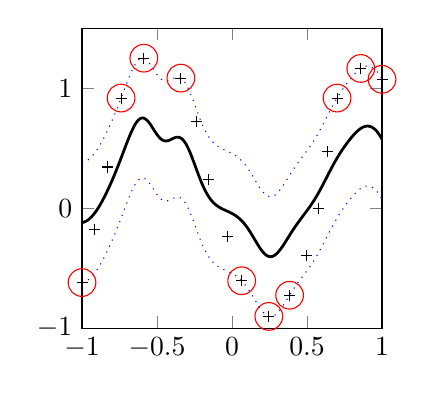
\begin{tikzpicture}

\begin{axis}[%
width=1.5in,
height=1.5in,
scale only axis,
xmin=-1,
xmax=1,
ymin=-1,
ymax=1.5,
]
\addplot [color=black,solid,line width=1.0pt,forget plot]
  table[row sep=crcr]{%
-1	-0.119455645186418\\
-0.993333333333333	-0.117782315701881\\
-0.986666666666667	-0.115330439070124\\
-0.98	-0.112085410918312\\
-0.973333333333333	-0.108038333412802\\
-0.966666666666667	-0.103185792949165\\
-0.96	-0.0975295395652418\\
-0.953333333333333	-0.091076083602175\\
-0.946666666666667	-0.0838362270005101\\
-0.94	-0.075824547580335\\
-0.933333333333333	-0.0670588546991235\\
-0.926666666666667	-0.057559633847747\\
-0.92	-0.0473494961282862\\
-0.913333333333333	-0.0364526463011332\\
-0.906666666666667	-0.0248943803794624\\
-0.9	-0.01270062080266\\
-0.893333333333333	0.000102505730774013\\
-0.886666666666667	0.0134890454130289\\
-0.88	0.0274335493789692\\
-0.873333333333333	0.0419113622268442\\
-0.866666666666667	0.0568988694534322\\
-0.86	0.0723737062824397\\
-0.853333333333333	0.0883149295425906\\
-0.846666666666667	0.104703152638042\\
-0.84	0.121520641386153\\
-0.833333333333333	0.138751365782292\\
-0.826666666666667	0.156380999852549\\
-0.82	0.174396858980029\\
-0.813333333333333	0.19278776176988\\
-0.806666666666667	0.211543801984328\\
-0.8	0.230656015640675\\
-0.793333333333333	0.250115929283309\\
-0.786666666666667	0.26991497790457\\
-0.78	0.290043785095808\\
-0.773333333333333	0.310491303747913\\
-0.766666666666667	0.331243822860176\\
-0.76	0.352283854506237\\
-0.753333333333333	0.373588924377962\\
-0.746666666666667	0.395130299110457\\
-0.74	0.416871693228989\\
-0.733333333333333	0.438768007441051\\
-0.726666666666667	0.460764157492252\\
-0.72	0.482794058297092\\
-0.713333333333333	0.504779830984181\\
-0.706666666666667	0.526631300393405\\
-0.7	0.548245847092743\\
-0.693333333333333	0.569508670967361\\
-0.686666666666667	0.590293512877499\\
-0.68	0.610463866983062\\
-0.673333333333333	0.629874699486165\\
-0.666666666666667	0.648374670328512\\
-0.66	0.665808833543377\\
-0.653333333333333	0.68202177037964\\
-0.646666666666667	0.696861087956775\\
-0.64	0.710181196087799\\
-0.633333333333333	0.721847257026299\\
-0.626666666666667	0.73173918819677\\
-0.62	0.739755587284916\\
-0.613333333333333	0.745817443067874\\
-0.606666666666667	0.749871494528023\\
-0.6	0.751893105367408\\
-0.593333333333333	0.751888531030694\\
-0.586666666666667	0.749896470515271\\
-0.58	0.745988815124161\\
-0.573333333333333	0.740270530212236\\
-0.566666666666667	0.732878633017899\\
-0.56	0.723980258848051\\
-0.553333333333333	0.713769838086412\\
-0.546666666666667	0.702465436573026\\
-0.54	0.690304340712338\\
-0.533333333333333	0.677537995122203\\
-0.526666666666667	0.664426423751577\\
-0.52	0.651232284326113\\
-0.513333333333333	0.638214720054022\\
-0.506666666666667	0.625623181257031\\
-0.5	0.613691392704012\\
-0.493333333333333	0.602631639845737\\
-0.486666666666667	0.592629539006687\\
-0.48	0.583839443201083\\
-0.473333333333333	0.576380617091588\\
-0.466666666666667	0.570334292333024\\
-0.46	0.565741688892053\\
-0.453333333333333	0.562603059750499\\
-0.446666666666667	0.560877786590215\\
-0.44	0.560485523559982\\
-0.433333333333333	0.561308355983594\\
-0.426666666666667	0.563193911805313\\
-0.42	0.565959336559459\\
-0.413333333333333	0.569396018500052\\
-0.406666666666667	0.573274929947028\\
-0.4	0.577352434499204\\
-0.393333333333333	0.581376398004014\\
-0.386666666666667	0.585092434390099\\
-0.38	0.588250115837417\\
-0.373333333333333	0.590608980295124\\
-0.366666666666667	0.591944177910489\\
-0.36	0.59205161119024\\
-0.353333333333333	0.59075244121201\\
-0.346666666666667	0.58789685332892\\
-0.34	0.583366999833418\\
-0.333333333333333	0.577079063137188\\
-0.326666666666667	0.568984410283569\\
-0.32	0.559069837102688\\
-0.313333333333333	0.547356927112577\\
-0.306666666666667	0.533900575463401\\
-0.3	0.518786750989972\\
-0.293333333333333	0.502129589058734\\
-0.286666666666667	0.484067923781589\\
-0.28	0.464761379889162\\
-0.273333333333333	0.44438615185095\\
-0.266666666666667	0.423130600619132\\
-0.26	0.401190796754664\\
-0.253333333333333	0.378766132935151\\
-0.246666666666667	0.356055119361915\\
-0.24	0.333251462923946\\
-0.233333333333333	0.310540515782379\\
-0.226666666666667	0.288096162019318\\
-0.22	0.266078192888303\\
-0.213333333333333	0.244630202745744\\
-0.206666666666667	0.223878019632282\\
-0.2	0.203928667344473\\
-0.193333333333333	0.184869840236246\\
-0.186666666666667	0.166769858355629\\
-0.18	0.149678059177721\\
-0.173333333333333	0.133625573340254\\
-0.166666666666667	0.118626425504298\\
-0.16	0.104678897718808\\
-0.153333333333333	0.0917670913338046\\
-0.146666666666667	0.0798626243704002\\
-0.14	0.0689264040407239\\
-0.133333333333333	0.0589104184974292\\
-0.126666666666667	0.0497594975386065\\
-0.12	0.0414129985527661\\
-0.113333333333333	0.033806381126231\\
-0.106666666666667	0.026872641144493\\
-0.1	0.0205435826297871\\
-0.0933333333333333	0.0147509127434772\\
-0.0866666666666666	0.00942715216551302\\
-0.08	0.00450635931335585\\
-0.0733333333333333	-7.53275069385247e-05\\
-0.0666666666666667	-0.00437932096168202\\
-0.0599999999999999	-0.00846437522626724\\
-0.0533333333333332	-0.012386519255251\\
-0.0466666666666666	-0.016199112888494\\
-0.0399999999999999	-0.019953003562107\\
-0.0333333333333333	-0.0236967596502722\\
-0.0266666666666666	-0.0274769552890359\\
-0.0199999999999999	-0.0313384809125136\\
-0.0133333333333333	-0.0353248536643514\\
-0.0066666666666666	-0.039478502343322\\
1.11022302462516e-16	-0.0438410026217969\\
0.00666666666666682	-0.048453239965113\\
0.0133333333333335	-0.0533554800038981\\
0.0200000000000001	-0.0585873290885842\\
0.0266666666666668	-0.0641875713896833\\
0.0333333333333335	-0.0701938731815121\\
0.0400000000000001	-0.0766423498154645\\
0.0466666666666669	-0.0835669962728895\\
0.0533333333333335	-0.0909989879716797\\
0.0600000000000002	-0.0989658645315155\\
0.0666666666666669	-0.107490615290716\\
0.0733333333333335	-0.11659069129129\\
0.0800000000000002	-0.126276973961771\\
0.0866666666666668	-0.136552735568586\\
0.0933333333333335	-0.147412630412485\\
0.1	-0.158841758464281\\
0.106666666666667	-0.170814844438098\\
0.113333333333334	-0.183295575005668\\
0.12	-0.196236134833465\\
0.126666666666667	-0.209576978315352\\
0.133333333333334	-0.223246868295215\\
0.14	-0.237163205829566\\
0.146666666666667	-0.251232666318994\\
0.153333333333334	-0.265352147413087\\
0.16	-0.279410023315757\\
0.166666666666667	-0.293287688900044\\
0.173333333333333	-0.306861365843147\\
0.18	-0.320004132298875\\
0.186666666666667	-0.332588127923231\\
0.193333333333333	-0.344486877823518\\
0.2	-0.355577672628233\\
0.206666666666667	-0.365743937718119\\
0.213333333333333	-0.374877522969758\\
0.22	-0.382880845284468\\
0.226666666666667	-0.38966881973005\\
0.233333333333334	-0.395170521209322\\
0.24	-0.399330526963874\\
0.246666666666667	-0.402109900587271\\
0.253333333333334	-0.403486790125066\\
0.26	-0.403456625769356\\
0.266666666666667	-0.402031916053096\\
0.273333333333334	-0.399241654732547\\
0.28	-0.395130363142559\\
0.286666666666667	-0.389756804185485\\
0.293333333333334	-0.383192413802803\\
0.3	-0.375519503401868\\
0.306666666666667	-0.366829291999517\\
0.313333333333333	-0.357219829650788\\
0.32	-0.346793874031548\\
0.326666666666667	-0.335656779938179\\
0.333333333333333	-0.32391445716986\\
0.34	-0.311671446082329\\
0.346666666666667	-0.299029152438093\\
0.353333333333333	-0.286084274472674\\
0.36	-0.272927445823898\\
0.366666666666667	-0.259642108606388\\
0.373333333333334	-0.246303621906713\\
0.38	-0.23297860272834\\
0.386666666666667	-0.219724489264122\\
0.393333333333334	-0.2065893105698\\
0.4	-0.193611642415562\\
0.406666666666667	-0.180820726369247\\
0.413333333333334	-0.168236727986531\\
0.42	-0.155871110236275\\
0.426666666666667	-0.14372709978475\\
0.433333333333334	-0.13180022625309\\
0.44	-0.120078917758941\\
0.446666666666667	-0.108545139644633\\
0.453333333333333	-0.0971750669658272\\
0.46	-0.0859397847678603\\
0.466666666666667	-0.0748060131455951\\
0.473333333333333	-0.0637368563468336\\
0.48	-0.0526925765775723\\
0.486666666666667	-0.0416313936033107\\
0.493333333333334	-0.0305103106874898\\
0.5	-0.0192859659088004\\
0.506666666666667	-0.00791550556255729\\
0.513333333333334	0.00364252665392176\\
0.52	0.0154272944278601\\
0.526666666666667	0.0274747809962504\\
0.533333333333334	0.0398169256633196\\
0.54	0.052480804839584\\
0.546666666666667	0.0654878803178186\\
0.553333333333333	0.0788533391427194\\
0.56	0.0925855499527725\\
0.566666666666667	0.106685659912984\\
0.573333333333333	0.121147354218852\\
0.58	0.135956796612448\\
0.586666666666667	0.151092764467514\\
0.593333333333333	0.166526985910058\\
0.6	0.182224679360812\\
0.606666666666667	0.198145288104737\\
0.613333333333334	0.214243394359575\\
0.62	0.230469789224617\\
0.626666666666667	0.246772667262835\\
0.633333333333334	0.263098907729213\\
0.64	0.279395399011366\\
0.646666666666667	0.295610359057875\\
0.653333333333334	0.311694602731365\\
0.66	0.327602707345628\\
0.666666666666667	0.343294030232874\\
0.673333333333334	0.358733537024888\\
0.68	0.373892406283911\\
0.686666666666667	0.38874838492615\\
0.693333333333334	0.403285879169928\\
0.7	0.41749577703963\\
0.706666666666667	0.431375010218186\\
0.713333333333334	0.444925874669432\\
0.72	0.458155140337119\\
0.726666666666667	0.471072989779814\\
0.733333333333334	0.483691833287046\\
0.74	0.496025053398214\\
0.746666666666667	0.508085734488526\\
0.753333333333334	0.519885433014964\\
0.76	0.531433041108075\\
0.766666666666667	0.542733790594668\\
0.773333333333334	0.553788436544347\\
0.78	0.564592649496857\\
0.786666666666667	0.57513663421551\\
0.793333333333334	0.585404980780561\\
0.8	0.595376741789799\\
0.806666666666667	0.605025718081221\\
0.813333333333334	0.614320925404148\\
0.82	0.623227206427373\\
0.826666666666667	0.631705946851464\\
0.833333333333333	0.639715851500517\\
0.84	0.647213736245744\\
0.846666666666667	0.654155294414668\\
0.853333333333333	0.660495801738131\\
0.86	0.666190731487306\\
0.866666666666667	0.671196260715724\\
0.873333333333334	0.67546965880019\\
0.88	0.678969560057188\\
0.886666666666667	0.681656132367196\\
0.893333333333334	0.683491162768021\\
0.9	0.684438088256166\\
0.906666666666667	0.684462005057513\\
0.913333333333334	0.683529692042348\\
0.92	0.681609683587682\\
0.926666666666667	0.678672424041594\\
0.933333333333334	0.67469053021575\\
0.94	0.669639180391259\\
0.946666666666667	0.663496638685388\\
0.953333333333334	0.656244912920512\\
0.96	0.647870533061431\\
0.966666666666667	0.638365426566807\\
0.973333333333334	0.627727857336638\\
0.98	0.615963386964431\\
0.986666666666667	0.603085811246548\\
0.993333333333334	0.589118021748848\\
1	0.574092741906371\\
};
\addplot [color=blue,dotted,forget plot]
  table[row sep=crcr]{%
-1	0.380544354813582\\
-0.993333333333333	0.382217684298119\\
-0.986666666666667	0.384669560929876\\
-0.98	0.387914589081688\\
-0.973333333333333	0.391961666587198\\
-0.966666666666667	0.396814207050835\\
-0.96	0.402470460434758\\
-0.953333333333333	0.408923916397825\\
-0.946666666666667	0.41616377299949\\
-0.94	0.424175452419665\\
-0.933333333333333	0.432941145300877\\
-0.926666666666667	0.442440366152253\\
-0.92	0.452650503871714\\
-0.913333333333333	0.463547353698867\\
-0.906666666666667	0.475105619620538\\
-0.9	0.48729937919734\\
-0.893333333333333	0.500102505730774\\
-0.886666666666667	0.513489045413029\\
-0.88	0.527433549378969\\
-0.873333333333333	0.541911362226844\\
-0.866666666666667	0.556898869453432\\
-0.86	0.57237370628244\\
-0.853333333333333	0.588314929542591\\
-0.846666666666667	0.604703152638042\\
-0.84	0.621520641386153\\
-0.833333333333333	0.638751365782292\\
-0.826666666666667	0.656380999852549\\
-0.82	0.674396858980029\\
-0.813333333333333	0.69278776176988\\
-0.806666666666667	0.711543801984328\\
-0.8	0.730656015640675\\
-0.793333333333333	0.750115929283309\\
-0.786666666666667	0.76991497790457\\
-0.78	0.790043785095808\\
-0.773333333333333	0.810491303747913\\
-0.766666666666667	0.831243822860176\\
-0.76	0.852283854506237\\
-0.753333333333333	0.873588924377962\\
-0.746666666666667	0.895130299110457\\
-0.74	0.91687169322899\\
-0.733333333333333	0.93876800744105\\
-0.726666666666667	0.960764157492252\\
-0.72	0.982794058297092\\
-0.713333333333333	1.00477983098418\\
-0.706666666666667	1.02663130039341\\
-0.7	1.04824584709274\\
-0.693333333333333	1.06950867096736\\
-0.686666666666667	1.0902935128775\\
-0.68	1.11046386698306\\
-0.673333333333333	1.12987469948617\\
-0.666666666666667	1.14837467032851\\
-0.66	1.16580883354338\\
-0.653333333333333	1.18202177037964\\
-0.646666666666667	1.19686108795677\\
-0.64	1.2101811960878\\
-0.633333333333333	1.2218472570263\\
-0.626666666666667	1.23173918819677\\
-0.62	1.23975558728492\\
-0.613333333333333	1.24581744306787\\
-0.606666666666667	1.24987149452802\\
-0.6	1.25189310536741\\
-0.593333333333333	1.25188853103069\\
-0.586666666666667	1.24989647051527\\
-0.58	1.24598881512416\\
-0.573333333333333	1.24027053021224\\
-0.566666666666667	1.2328786330179\\
-0.56	1.22398025884805\\
-0.553333333333333	1.21376983808641\\
-0.546666666666667	1.20246543657303\\
-0.54	1.19030434071234\\
-0.533333333333333	1.1775379951222\\
-0.526666666666667	1.16442642375158\\
-0.52	1.15123228432611\\
-0.513333333333333	1.13821472005402\\
-0.506666666666667	1.12562318125703\\
-0.5	1.11369139270401\\
-0.493333333333333	1.10263163984574\\
-0.486666666666667	1.09262953900669\\
-0.48	1.08383944320108\\
-0.473333333333333	1.07638061709159\\
-0.466666666666667	1.07033429233302\\
-0.46	1.06574168889205\\
-0.453333333333333	1.0626030597505\\
-0.446666666666667	1.06087778659022\\
-0.44	1.06048552355998\\
-0.433333333333333	1.06130835598359\\
-0.426666666666667	1.06319391180531\\
-0.42	1.06595933655946\\
-0.413333333333333	1.06939601850005\\
-0.406666666666667	1.07327492994703\\
-0.4	1.0773524344992\\
-0.393333333333333	1.08137639800401\\
-0.386666666666667	1.0850924343901\\
-0.38	1.08825011583742\\
-0.373333333333333	1.09060898029512\\
-0.366666666666667	1.09194417791049\\
-0.36	1.09205161119024\\
-0.353333333333333	1.09075244121201\\
-0.346666666666667	1.08789685332892\\
-0.34	1.08336699983342\\
-0.333333333333333	1.07707906313719\\
-0.326666666666667	1.06898441028357\\
-0.32	1.05906983710269\\
-0.313333333333333	1.04735692711258\\
-0.306666666666667	1.0339005754634\\
-0.3	1.01878675098997\\
-0.293333333333333	1.00212958905873\\
-0.286666666666667	0.984067923781589\\
-0.28	0.964761379889162\\
-0.273333333333333	0.94438615185095\\
-0.266666666666667	0.923130600619132\\
-0.26	0.901190796754664\\
-0.253333333333333	0.878766132935151\\
-0.246666666666667	0.856055119361915\\
-0.24	0.833251462923946\\
-0.233333333333333	0.810540515782379\\
-0.226666666666667	0.788096162019318\\
-0.22	0.766078192888303\\
-0.213333333333333	0.744630202745745\\
-0.206666666666667	0.723878019632282\\
-0.2	0.703928667344473\\
-0.193333333333333	0.684869840236246\\
-0.186666666666667	0.666769858355629\\
-0.18	0.649678059177721\\
-0.173333333333333	0.633625573340254\\
-0.166666666666667	0.618626425504298\\
-0.16	0.604678897718808\\
-0.153333333333333	0.591767091333805\\
-0.146666666666667	0.5798626243704\\
-0.14	0.568926404040724\\
-0.133333333333333	0.558910418497429\\
-0.126666666666667	0.549759497538606\\
-0.12	0.541412998552766\\
-0.113333333333333	0.533806381126231\\
-0.106666666666667	0.526872641144493\\
-0.1	0.520543582629787\\
-0.0933333333333333	0.514750912743477\\
-0.0866666666666666	0.509427152165513\\
-0.08	0.504506359313356\\
-0.0733333333333333	0.499924672493061\\
-0.0666666666666667	0.495620679038318\\
-0.0599999999999999	0.491535624773733\\
-0.0533333333333332	0.487613480744749\\
-0.0466666666666666	0.483800887111506\\
-0.0399999999999999	0.480046996437893\\
-0.0333333333333333	0.476303240349728\\
-0.0266666666666666	0.472523044710964\\
-0.0199999999999999	0.468661519087486\\
-0.0133333333333333	0.464675146335649\\
-0.0066666666666666	0.460521497656678\\
1.11022302462516e-16	0.456158997378203\\
0.00666666666666682	0.451546760034887\\
0.0133333333333335	0.446644519996102\\
0.0200000000000001	0.441412670911416\\
0.0266666666666668	0.435812428610317\\
0.0333333333333335	0.429806126818488\\
0.0400000000000001	0.423357650184535\\
0.0466666666666669	0.41643300372711\\
0.0533333333333335	0.40900101202832\\
0.0600000000000002	0.401034135468485\\
0.0666666666666669	0.392509384709284\\
0.0733333333333335	0.38340930870871\\
0.0800000000000002	0.373723026038229\\
0.0866666666666668	0.363447264431414\\
0.0933333333333335	0.352587369587515\\
0.1	0.341158241535719\\
0.106666666666667	0.329185155561902\\
0.113333333333334	0.316704424994331\\
0.12	0.303763865166535\\
0.126666666666667	0.290423021684648\\
0.133333333333334	0.276753131704785\\
0.14	0.262836794170434\\
0.146666666666667	0.248767333681006\\
0.153333333333334	0.234647852586913\\
0.16	0.220589976684243\\
0.166666666666667	0.206712311099956\\
0.173333333333333	0.193138634156853\\
0.18	0.179995867701125\\
0.186666666666667	0.167411872076769\\
0.193333333333333	0.155513122176482\\
0.2	0.144422327371767\\
0.206666666666667	0.134256062281881\\
0.213333333333333	0.125122477030242\\
0.22	0.117119154715532\\
0.226666666666667	0.11033118026995\\
0.233333333333334	0.104829478790678\\
0.24	0.100669473036126\\
0.246666666666667	0.0978900994127292\\
0.253333333333334	0.0965132098749337\\
0.26	0.0965433742306445\\
0.266666666666667	0.0979680839469035\\
0.273333333333334	0.100758345267453\\
0.28	0.104869636857441\\
0.286666666666667	0.110243195814515\\
0.293333333333334	0.116807586197197\\
0.3	0.124480496598132\\
0.306666666666667	0.133170708000483\\
0.313333333333333	0.142780170349212\\
0.32	0.153206125968452\\
0.326666666666667	0.164343220061821\\
0.333333333333333	0.17608554283014\\
0.34	0.188328553917671\\
0.346666666666667	0.200970847561907\\
0.353333333333333	0.213915725527326\\
0.36	0.227072554176102\\
0.366666666666667	0.240357891393612\\
0.373333333333334	0.253696378093287\\
0.38	0.26702139727166\\
0.386666666666667	0.280275510735878\\
0.393333333333334	0.2934106894302\\
0.4	0.306388357584438\\
0.406666666666667	0.319179273630753\\
0.413333333333334	0.331763272013469\\
0.42	0.344128889763725\\
0.426666666666667	0.35627290021525\\
0.433333333333334	0.36819977374691\\
0.44	0.379921082241059\\
0.446666666666667	0.391454860355367\\
0.453333333333333	0.402824933034173\\
0.46	0.41406021523214\\
0.466666666666667	0.425193986854405\\
0.473333333333333	0.436263143653166\\
0.48	0.447307423422428\\
0.486666666666667	0.458368606396689\\
0.493333333333334	0.46948968931251\\
0.5	0.4807140340912\\
0.506666666666667	0.492084494437443\\
0.513333333333334	0.503642526653922\\
0.52	0.51542729442786\\
0.526666666666667	0.52747478099625\\
0.533333333333334	0.53981692566332\\
0.54	0.552480804839584\\
0.546666666666667	0.565487880317819\\
0.553333333333333	0.578853339142719\\
0.56	0.592585549952773\\
0.566666666666667	0.606685659912984\\
0.573333333333333	0.621147354218852\\
0.58	0.635956796612448\\
0.586666666666667	0.651092764467514\\
0.593333333333333	0.666526985910058\\
0.6	0.682224679360812\\
0.606666666666667	0.698145288104737\\
0.613333333333334	0.714243394359575\\
0.62	0.730469789224617\\
0.626666666666667	0.746772667262835\\
0.633333333333334	0.763098907729213\\
0.64	0.779395399011366\\
0.646666666666667	0.795610359057875\\
0.653333333333334	0.811694602731365\\
0.66	0.827602707345628\\
0.666666666666667	0.843294030232874\\
0.673333333333334	0.858733537024888\\
0.68	0.873892406283911\\
0.686666666666667	0.88874838492615\\
0.693333333333334	0.903285879169928\\
0.7	0.91749577703963\\
0.706666666666667	0.931375010218186\\
0.713333333333334	0.944925874669432\\
0.72	0.958155140337119\\
0.726666666666667	0.971072989779814\\
0.733333333333334	0.983691833287046\\
0.74	0.996025053398214\\
0.746666666666667	1.00808573448853\\
0.753333333333334	1.01988543301496\\
0.76	1.03143304110808\\
0.766666666666667	1.04273379059467\\
0.773333333333334	1.05378843654435\\
0.78	1.06459264949686\\
0.786666666666667	1.07513663421551\\
0.793333333333334	1.08540498078056\\
0.8	1.0953767417898\\
0.806666666666667	1.10502571808122\\
0.813333333333334	1.11432092540415\\
0.82	1.12322720642737\\
0.826666666666667	1.13170594685146\\
0.833333333333333	1.13971585150052\\
0.84	1.14721373624574\\
0.846666666666667	1.15415529441467\\
0.853333333333333	1.16049580173813\\
0.86	1.16619073148731\\
0.866666666666667	1.17119626071572\\
0.873333333333334	1.17546965880019\\
0.88	1.17896956005719\\
0.886666666666667	1.1816561323672\\
0.893333333333334	1.18349116276802\\
0.9	1.18443808825617\\
0.906666666666667	1.18446200505751\\
0.913333333333334	1.18352969204235\\
0.92	1.18160968358768\\
0.926666666666667	1.17867242404159\\
0.933333333333334	1.17469053021575\\
0.94	1.16963918039126\\
0.946666666666667	1.16349663868539\\
0.953333333333334	1.15624491292051\\
0.96	1.14787053306143\\
0.966666666666667	1.13836542656681\\
0.973333333333334	1.12772785733664\\
0.98	1.11596338696443\\
0.986666666666667	1.10308581124655\\
0.993333333333334	1.08911802174885\\
1	1.07409274190637\\
};
\addplot [color=blue,dotted,forget plot]
  table[row sep=crcr]{%
-1	-0.619455645186418\\
-0.993333333333333	-0.617782315701881\\
-0.986666666666667	-0.615330439070124\\
-0.98	-0.612085410918312\\
-0.973333333333333	-0.608038333412802\\
-0.966666666666667	-0.603185792949165\\
-0.96	-0.597529539565242\\
-0.953333333333333	-0.591076083602175\\
-0.946666666666667	-0.58383622700051\\
-0.94	-0.575824547580335\\
-0.933333333333333	-0.567058854699124\\
-0.926666666666667	-0.557559633847747\\
-0.92	-0.547349496128286\\
-0.913333333333333	-0.536452646301133\\
-0.906666666666667	-0.524894380379462\\
-0.9	-0.51270062080266\\
-0.893333333333333	-0.499897494269226\\
-0.886666666666667	-0.486510954586971\\
-0.88	-0.472566450621031\\
-0.873333333333333	-0.458088637773156\\
-0.866666666666667	-0.443101130546568\\
-0.86	-0.42762629371756\\
-0.853333333333333	-0.411685070457409\\
-0.846666666666667	-0.395296847361958\\
-0.84	-0.378479358613847\\
-0.833333333333333	-0.361248634217708\\
-0.826666666666667	-0.343619000147451\\
-0.82	-0.325603141019971\\
-0.813333333333333	-0.30721223823012\\
-0.806666666666667	-0.288456198015672\\
-0.8	-0.269343984359325\\
-0.793333333333333	-0.249884070716691\\
-0.786666666666667	-0.23008502209543\\
-0.78	-0.209956214904192\\
-0.773333333333333	-0.189508696252087\\
-0.766666666666667	-0.168756177139824\\
-0.76	-0.147716145493763\\
-0.753333333333333	-0.126411075622038\\
-0.746666666666667	-0.104869700889543\\
-0.74	-0.0831283067710105\\
-0.733333333333333	-0.0612319925589495\\
-0.726666666666667	-0.0392358425077485\\
-0.72	-0.017205941702908\\
-0.713333333333333	0.00477983098418133\\
-0.706666666666667	0.0266313003934053\\
-0.7	0.0482458470927433\\
-0.693333333333333	0.069508670967361\\
-0.686666666666667	0.0902935128774985\\
-0.68	0.110463866983062\\
-0.673333333333333	0.129874699486165\\
-0.666666666666667	0.148374670328512\\
-0.66	0.165808833543377\\
-0.653333333333333	0.18202177037964\\
-0.646666666666667	0.196861087956775\\
-0.64	0.210181196087799\\
-0.633333333333333	0.221847257026299\\
-0.626666666666667	0.23173918819677\\
-0.62	0.239755587284916\\
-0.613333333333333	0.245817443067874\\
-0.606666666666667	0.249871494528023\\
-0.6	0.251893105367408\\
-0.593333333333333	0.251888531030694\\
-0.586666666666667	0.249896470515271\\
-0.58	0.245988815124161\\
-0.573333333333333	0.240270530212236\\
-0.566666666666667	0.232878633017899\\
-0.56	0.223980258848051\\
-0.553333333333333	0.213769838086412\\
-0.546666666666667	0.202465436573026\\
-0.54	0.190304340712338\\
-0.533333333333333	0.177537995122203\\
-0.526666666666667	0.164426423751577\\
-0.52	0.151232284326113\\
-0.513333333333333	0.138214720054022\\
-0.506666666666667	0.125623181257031\\
-0.5	0.113691392704012\\
-0.493333333333333	0.102631639845737\\
-0.486666666666667	0.092629539006687\\
-0.48	0.0838394432010826\\
-0.473333333333333	0.0763806170915878\\
-0.466666666666667	0.0703342923330237\\
-0.46	0.0657416888920531\\
-0.453333333333333	0.0626030597504994\\
-0.446666666666667	0.0608777865902153\\
-0.44	0.0604855235599816\\
-0.433333333333333	0.061308355983594\\
-0.426666666666667	0.0631939118053134\\
-0.42	0.0659593365594591\\
-0.413333333333333	0.0693960185000522\\
-0.406666666666667	0.0732749299470277\\
-0.4	0.0773524344992043\\
-0.393333333333333	0.0813763980040139\\
-0.386666666666667	0.0850924343900987\\
-0.38	0.0882501158374168\\
-0.373333333333333	0.0906089802951244\\
-0.366666666666667	0.0919441779104887\\
-0.36	0.0920516111902403\\
-0.353333333333333	0.0907524412120104\\
-0.346666666666667	0.0878968533289203\\
-0.34	0.0833669998334177\\
-0.333333333333333	0.0770790631371876\\
-0.326666666666667	0.0689844102835695\\
-0.32	0.0590698371026884\\
-0.313333333333333	0.0473569271125772\\
-0.306666666666667	0.033900575463401\\
-0.3	0.0187867509899718\\
-0.293333333333333	0.00212958905873384\\
-0.286666666666667	-0.0159320762184114\\
-0.28	-0.0352386201108378\\
-0.273333333333333	-0.0556138481490497\\
-0.266666666666667	-0.0768693993808683\\
-0.26	-0.0988092032453363\\
-0.253333333333333	-0.121233867064849\\
-0.246666666666667	-0.143944880638085\\
-0.24	-0.166748537076054\\
-0.233333333333333	-0.189459484217621\\
-0.226666666666667	-0.211903837980682\\
-0.22	-0.233921807111697\\
-0.213333333333333	-0.255369797254256\\
-0.206666666666667	-0.276121980367718\\
-0.2	-0.296071332655527\\
-0.193333333333333	-0.315130159763754\\
-0.186666666666667	-0.333230141644371\\
-0.18	-0.350321940822279\\
-0.173333333333333	-0.366374426659746\\
-0.166666666666667	-0.381373574495702\\
-0.16	-0.395321102281192\\
-0.153333333333333	-0.408232908666195\\
-0.146666666666667	-0.4201373756296\\
-0.14	-0.431073595959276\\
-0.133333333333333	-0.441089581502571\\
-0.126666666666667	-0.450240502461394\\
-0.12	-0.458587001447234\\
-0.113333333333333	-0.466193618873769\\
-0.106666666666667	-0.473127358855507\\
-0.1	-0.479456417370213\\
-0.0933333333333333	-0.485249087256523\\
-0.0866666666666666	-0.490572847834487\\
-0.08	-0.495493640686644\\
-0.0733333333333333	-0.500075327506939\\
-0.0666666666666667	-0.504379320961682\\
-0.0599999999999999	-0.508464375226267\\
-0.0533333333333332	-0.512386519255251\\
-0.0466666666666666	-0.516199112888494\\
-0.0399999999999999	-0.519953003562107\\
-0.0333333333333333	-0.523696759650272\\
-0.0266666666666666	-0.527476955289036\\
-0.0199999999999999	-0.531338480912514\\
-0.0133333333333333	-0.535324853664351\\
-0.0066666666666666	-0.539478502343322\\
1.11022302462516e-16	-0.543841002621797\\
0.00666666666666682	-0.548453239965113\\
0.0133333333333335	-0.553355480003898\\
0.0200000000000001	-0.558587329088584\\
0.0266666666666668	-0.564187571389683\\
0.0333333333333335	-0.570193873181512\\
0.0400000000000001	-0.576642349815465\\
0.0466666666666669	-0.58356699627289\\
0.0533333333333335	-0.59099898797168\\
0.0600000000000002	-0.598965864531515\\
0.0666666666666669	-0.607490615290716\\
0.0733333333333335	-0.616590691291291\\
0.0800000000000002	-0.626276973961771\\
0.0866666666666668	-0.636552735568586\\
0.0933333333333335	-0.647412630412485\\
0.1	-0.658841758464281\\
0.106666666666667	-0.670814844438098\\
0.113333333333334	-0.683295575005669\\
0.12	-0.696236134833465\\
0.126666666666667	-0.709576978315352\\
0.133333333333334	-0.723246868295215\\
0.14	-0.737163205829566\\
0.146666666666667	-0.751232666318994\\
0.153333333333334	-0.765352147413087\\
0.16	-0.779410023315757\\
0.166666666666667	-0.793287688900044\\
0.173333333333333	-0.806861365843147\\
0.18	-0.820004132298875\\
0.186666666666667	-0.832588127923231\\
0.193333333333333	-0.844486877823518\\
0.2	-0.855577672628233\\
0.206666666666667	-0.865743937718119\\
0.213333333333333	-0.874877522969758\\
0.22	-0.882880845284468\\
0.226666666666667	-0.88966881973005\\
0.233333333333334	-0.895170521209322\\
0.24	-0.899330526963874\\
0.246666666666667	-0.902109900587271\\
0.253333333333334	-0.903486790125066\\
0.26	-0.903456625769355\\
0.266666666666667	-0.902031916053097\\
0.273333333333334	-0.899241654732547\\
0.28	-0.895130363142558\\
0.286666666666667	-0.889756804185485\\
0.293333333333334	-0.883192413802803\\
0.3	-0.875519503401868\\
0.306666666666667	-0.866829291999517\\
0.313333333333333	-0.857219829650788\\
0.32	-0.846793874031548\\
0.326666666666667	-0.83565677993818\\
0.333333333333333	-0.82391445716986\\
0.34	-0.811671446082329\\
0.346666666666667	-0.799029152438093\\
0.353333333333333	-0.786084274472674\\
0.36	-0.772927445823898\\
0.366666666666667	-0.759642108606388\\
0.373333333333334	-0.746303621906713\\
0.38	-0.73297860272834\\
0.386666666666667	-0.719724489264122\\
0.393333333333334	-0.7065893105698\\
0.4	-0.693611642415562\\
0.406666666666667	-0.680820726369247\\
0.413333333333334	-0.668236727986531\\
0.42	-0.655871110236275\\
0.426666666666667	-0.64372709978475\\
0.433333333333334	-0.63180022625309\\
0.44	-0.620078917758941\\
0.446666666666667	-0.608545139644633\\
0.453333333333333	-0.597175066965827\\
0.46	-0.58593978476786\\
0.466666666666667	-0.574806013145595\\
0.473333333333333	-0.563736856346834\\
0.48	-0.552692576577572\\
0.486666666666667	-0.541631393603311\\
0.493333333333334	-0.53051031068749\\
0.5	-0.5192859659088\\
0.506666666666667	-0.507915505562557\\
0.513333333333334	-0.496357473346078\\
0.52	-0.48457270557214\\
0.526666666666667	-0.47252521900375\\
0.533333333333334	-0.46018307433668\\
0.54	-0.447519195160416\\
0.546666666666667	-0.434512119682181\\
0.553333333333333	-0.421146660857281\\
0.56	-0.407414450047227\\
0.566666666666667	-0.393314340087016\\
0.573333333333333	-0.378852645781148\\
0.58	-0.364043203387552\\
0.586666666666667	-0.348907235532486\\
0.593333333333333	-0.333473014089942\\
0.6	-0.317775320639188\\
0.606666666666667	-0.301854711895263\\
0.613333333333334	-0.285756605640425\\
0.62	-0.269530210775383\\
0.626666666666667	-0.253227332737165\\
0.633333333333334	-0.236901092270787\\
0.64	-0.220604600988634\\
0.646666666666667	-0.204389640942125\\
0.653333333333334	-0.188305397268635\\
0.66	-0.172397292654372\\
0.666666666666667	-0.156705969767126\\
0.673333333333334	-0.141266462975112\\
0.68	-0.126107593716089\\
0.686666666666667	-0.11125161507385\\
0.693333333333334	-0.096714120830072\\
0.7	-0.0825042229603701\\
0.706666666666667	-0.0686249897818144\\
0.713333333333334	-0.055074125330568\\
0.72	-0.0418448596628813\\
0.726666666666667	-0.0289270102201855\\
0.733333333333334	-0.0163081667129535\\
0.74	-0.00397494660178643\\
0.746666666666667	0.00808573448852601\\
0.753333333333334	0.0198854330149638\\
0.76	0.0314330411080752\\
0.766666666666667	0.0427337905946682\\
0.773333333333334	0.053788436544347\\
0.78	0.0645926494968569\\
0.786666666666667	0.0751366342155102\\
0.793333333333334	0.0854049807805614\\
0.8	0.095376741789799\\
0.806666666666667	0.105025718081221\\
0.813333333333334	0.114320925404148\\
0.82	0.123227206427373\\
0.826666666666667	0.131705946851464\\
0.833333333333333	0.139715851500517\\
0.84	0.147213736245744\\
0.846666666666667	0.154155294414668\\
0.853333333333333	0.160495801738131\\
0.86	0.166190731487306\\
0.866666666666667	0.171196260715724\\
0.873333333333334	0.17546965880019\\
0.88	0.178969560057188\\
0.886666666666667	0.181656132367196\\
0.893333333333334	0.183491162768021\\
0.9	0.184438088256166\\
0.906666666666667	0.184462005057513\\
0.913333333333334	0.183529692042348\\
0.92	0.181609683587682\\
0.926666666666667	0.178672424041594\\
0.933333333333334	0.17469053021575\\
0.94	0.169639180391259\\
0.946666666666667	0.163496638685388\\
0.953333333333334	0.156244912920512\\
0.96	0.147870533061431\\
0.966666666666667	0.138365426566807\\
0.973333333333334	0.127727857336638\\
0.98	0.115963386964431\\
0.986666666666667	0.103085811246548\\
0.993333333333334	0.0891180217488478\\
1	0.0740927419063715\\
};
\addplot [color=black,only marks,mark=+,mark options={solid},forget plot]
  table[row sep=crcr]{%
-1	-0.61945564516129\\
};
\addplot [color=red,mark size=5.0pt,only marks,mark=o,mark options={solid},forget plot]
  table[row sep=crcr]{%
-1	-0.61945564516129\\
};
\addplot [color=black,only marks,mark=+,mark options={solid},forget plot]
  table[row sep=crcr]{%
-0.917627677100494	-0.175907258064516\\
};
\addplot [color=black,only marks,mark=+,mark options={solid},forget plot]
  table[row sep=crcr]{%
-0.828665568369028	0.343245967741936\\
};
\addplot [color=black,only marks,mark=+,mark options={solid},forget plot]
  table[row sep=crcr]{%
-0.739703459637562	0.917842741935484\\
};
\addplot [color=red,mark size=5.0pt,only marks,mark=o,mark options={solid},forget plot]
  table[row sep=crcr]{%
-0.739703459637562	0.917842741935484\\
};
\addplot [color=black,only marks,mark=+,mark options={solid},forget plot]
  table[row sep=crcr]{%
-0.588138385502471	1.25050403225806\\
};
\addplot [color=red,mark size=5.0pt,only marks,mark=o,mark options={solid},forget plot]
  table[row sep=crcr]{%
-0.588138385502471	1.25050403225806\\
};
\addplot [color=black,only marks,mark=+,mark options={solid},forget plot]
  table[row sep=crcr]{%
-0.341021416803954	1.08417338709677\\
};
\addplot [color=red,mark size=5.0pt,only marks,mark=o,mark options={solid},forget plot]
  table[row sep=crcr]{%
-0.341021416803954	1.08417338709677\\
};
\addplot [color=black,only marks,mark=+,mark options={solid},forget plot]
  table[row sep=crcr]{%
-0.238879736408567	0.721270161290323\\
};
\addplot [color=black,only marks,mark=+,mark options={solid},forget plot]
  table[row sep=crcr]{%
-0.156507413509061	0.237399193548388\\
};
\addplot [color=black,only marks,mark=+,mark options={solid},forget plot]
  table[row sep=crcr]{%
-0.0280065897858319	-0.236391129032258\\
};
\addplot [color=black,only marks,mark=+,mark options={solid},forget plot]
  table[row sep=crcr]{%
0.0642504118616145	-0.604334677419354\\
};
\addplot [color=red,mark size=5.0pt,only marks,mark=o,mark options={solid},forget plot]
  table[row sep=crcr]{%
0.0642504118616145	-0.604334677419354\\
};
\addplot [color=black,only marks,mark=+,mark options={solid},forget plot]
  table[row sep=crcr]{%
0.245469522240527	-0.901713709677419\\
};
\addplot [color=red,mark size=5.0pt,only marks,mark=o,mark options={solid},forget plot]
  table[row sep=crcr]{%
0.245469522240527	-0.901713709677419\\
};
\addplot [color=black,only marks,mark=+,mark options={solid},forget plot]
  table[row sep=crcr]{%
0.383855024711697	-0.725302419354838\\
};
\addplot [color=red,mark size=5.0pt,only marks,mark=o,mark options={solid},forget plot]
  table[row sep=crcr]{%
0.383855024711697	-0.725302419354838\\
};
\addplot [color=black,only marks,mark=+,mark options={solid},forget plot]
  table[row sep=crcr]{%
0.495881383855025	-0.392641129032258\\
};
\addplot [color=black,only marks,mark=+,mark options={solid},forget plot]
  table[row sep=crcr]{%
0.574958813838551	0.000504032258065168\\
};
\addplot [color=black,only marks,mark=+,mark options={solid},forget plot]
  table[row sep=crcr]{%
0.634266886326194	0.469254032258065\\
};
\addplot [color=black,only marks,mark=+,mark options={solid},forget plot]
  table[row sep=crcr]{%
0.700164744645799	0.917842741935484\\
};
\addplot [color=red,mark size=5.0pt,only marks,mark=o,mark options={solid},forget plot]
  table[row sep=crcr]{%
0.700164744645799	0.917842741935484\\
};
\addplot [color=black,only marks,mark=+,mark options={solid},forget plot]
  table[row sep=crcr]{%
0.85831960461285	1.1648185483871\\
};
\addplot [color=red,mark size=5.0pt,only marks,mark=o,mark options={solid},forget plot]
  table[row sep=crcr]{%
0.85831960461285	1.1648185483871\\
};
\addplot [color=black,only marks,mark=+,mark options={solid},forget plot]
  table[row sep=crcr]{%
1	1.07409274193548\\
};
\addplot [color=red,mark size=5.0pt,only marks,mark=o,mark options={solid},forget plot]
  table[row sep=crcr]{%
1	1.07409274193548\\
};
\end{axis}
\end{tikzpicture}%
\end{document}
\caption{RBF kernel based funtion esimation with $\sigma^2 = 0.1$, $\epsilon = 0.1$, $\epsilon = 0.25$ and $\epsilon = 0.5$.}
\label{fig:ebfEstEps}
\end{figure}
\begin{figure}
\centering
% This file was created by matlab2tikz.
% Minimal pgfplots version: 1.3
%
%The latest updates can be retrieved from
%  http://www.mathworks.com/matlabcentral/fileexchange/22022-matlab2tikz
%where you can also make suggestions and rate matlab2tikz.
%
\documentclass[tikz]{standalone}
\usepackage{pgfplots}
\usepackage{grffile}
\pgfplotsset{compat=newest}
\usetikzlibrary{plotmarks}
\usepackage{amsmath}

\begin{document}
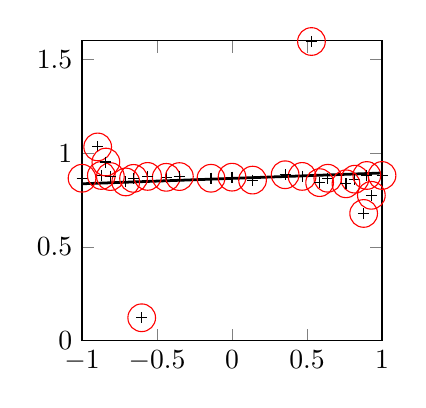
\begin{tikzpicture}

\begin{axis}[%
width=1.5in,
height=1.5in,
scale only axis,
xmin=-1,
xmax=1,
ymin=0,
ymax=1.6,
]
\addplot [color=black,solid,line width=1.0pt,forget plot]
  table[row sep=crcr]{%
-1	0.837249994277954\\
-0.993333333333333	0.837440013885498\\
-0.986666666666667	0.837631940841675\\
-0.98	0.837823987007141\\
-0.973333333333333	0.838015794754028\\
-0.966666666666667	0.838206052780151\\
-0.96	0.838399052619934\\
-0.953333333333333	0.838591694831848\\
-0.946666666666667	0.838783144950867\\
-0.94	0.838975548744202\\
-0.933333333333333	0.839166045188904\\
-0.926666666666667	0.839356899261475\\
-0.92	0.839550018310547\\
-0.913333333333333	0.839741468429565\\
-0.906666666666667	0.839932918548584\\
-0.9	0.840123414993286\\
-0.893333333333333	0.840316414833069\\
-0.886666666666667	0.840508222579956\\
-0.88	0.840698719024658\\
-0.873333333333333	0.840892553329468\\
-0.866666666666667	0.841084241867065\\
-0.86	0.841273903846741\\
-0.853333333333333	0.841467022895813\\
-0.846666666666667	0.841659426689148\\
-0.84	0.841850638389587\\
-0.833333333333333	0.842040181159973\\
-0.826666666666667	0.842234015464783\\
-0.82	0.842426896095276\\
-0.813333333333333	0.842616558074951\\
-0.806666666666667	0.84280800819397\\
-0.8	0.843000292778015\\
-0.793333333333333	0.843191742897034\\
-0.786666666666667	0.843384146690369\\
-0.78	0.843575119972229\\
-0.773333333333333	0.843768000602722\\
-0.766666666666667	0.843960046768188\\
-0.76	0.844151973724365\\
-0.753333333333333	0.844341993331909\\
-0.746666666666667	0.844535350799561\\
-0.74	0.844726920127869\\
-0.733333333333333	0.844918370246887\\
-0.726666666666667	0.845108270645142\\
-0.72	0.845302581787109\\
-0.713333333333333	0.845494151115417\\
-0.706666666666667	0.845685243606567\\
-0.7	0.845876216888428\\
-0.693333333333333	0.846069097518921\\
-0.686666666666667	0.846260190010071\\
-0.68	0.8464515209198\\
-0.673333333333333	0.846644401550293\\
-0.666666666666667	0.846835374832153\\
-0.66	0.847026467323303\\
-0.653333333333333	0.847220182418823\\
-0.646666666666667	0.847411394119263\\
-0.64	0.847602725028992\\
-0.633333333333333	0.847794413566589\\
-0.626666666666667	0.847987055778503\\
-0.62	0.848177075386047\\
-0.613333333333333	0.848368763923645\\
-0.606666666666667	0.848563432693481\\
-0.6	0.848753333091736\\
-0.593333333333333	0.848945379257202\\
-0.586666666666667	0.849136352539062\\
-0.58	0.849329352378845\\
-0.573333333333333	0.849520087242126\\
-0.566666666666667	0.849710881710052\\
-0.56	0.849902927875519\\
-0.553333333333333	0.850095212459564\\
-0.546666666666667	0.85028737783432\\
-0.54	0.850478827953339\\
-0.533333333333333	0.850669205188751\\
-0.526666666666667	0.850863456726074\\
-0.52	0.851053357124329\\
-0.513333333333333	0.851246416568756\\
-0.506666666666667	0.851436614990234\\
-0.5	0.851629853248596\\
-0.493333333333333	0.851821601390839\\
-0.486666666666667	0.852013051509857\\
-0.48	0.852204859256744\\
-0.473333333333333	0.852396428585052\\
-0.466666666666667	0.852588355541229\\
-0.46	0.852779626846313\\
-0.453333333333333	0.852970957756042\\
-0.446666666666667	0.853162586688995\\
-0.44	0.853354513645172\\
-0.433333333333333	0.853546500205994\\
-0.426666666666667	0.853738367557526\\
-0.42	0.853930413722992\\
-0.413333333333333	0.85412186384201\\
-0.406666666666667	0.854313433170319\\
-0.4	0.854504644870758\\
-0.393333333333333	0.854696452617645\\
-0.386666666666667	0.854889094829559\\
-0.38	0.855080842971802\\
-0.373333333333333	0.855272531509399\\
-0.366666666666667	0.855464279651642\\
-0.36	0.855655670166016\\
-0.353333333333333	0.855847716331482\\
-0.346666666666667	0.856038928031921\\
-0.34	0.856230616569519\\
-0.333333333333333	0.856422364711761\\
-0.326666666666667	0.856615424156189\\
-0.32	0.856806218624115\\
-0.313333333333333	0.856998205184937\\
-0.306666666666667	0.857189238071442\\
-0.3	0.857381463050842\\
-0.293333333333333	0.85757303237915\\
-0.286666666666667	0.857764899730682\\
-0.28	0.85795584321022\\
-0.273333333333333	0.858148545026779\\
-0.266666666666667	0.85833939909935\\
-0.26	0.858531892299652\\
-0.253333333333333	0.858723163604736\\
-0.246666666666667	0.858915656805038\\
-0.24	0.859106808900833\\
-0.233333333333333	0.859299063682556\\
-0.226666666666667	0.859490811824799\\
-0.22	0.859682112932205\\
-0.213333333333333	0.859874218702316\\
-0.206666666666667	0.860065788030624\\
-0.2	0.860257178544998\\
-0.193333333333333	0.860449343919754\\
-0.186666666666667	0.860641121864319\\
-0.18	0.860832810401917\\
-0.173333333333333	0.86102432012558\\
-0.166666666666667	0.8612160384655\\
-0.16	0.861407965421677\\
-0.153333333333333	0.86159947514534\\
-0.146666666666667	0.861791342496872\\
-0.14	0.861982792615891\\
-0.133333333333333	0.862174555659294\\
-0.126666666666667	0.862366363406181\\
-0.12	0.862558260560036\\
-0.113333333333333	0.862750023603439\\
-0.106666666666667	0.862941771745682\\
-0.1	0.863133445382118\\
-0.0933333333333333	0.863325208425522\\
-0.0866666666666666	0.863516807556152\\
-0.08	0.863708838820457\\
-0.0733333333333333	0.863900601863861\\
-0.0666666666666667	0.864092133939266\\
-0.0599999999999999	0.864284060895443\\
-0.0533333333333332	0.864475630223751\\
-0.0466666666666666	0.86466746032238\\
-0.0399999999999999	0.864859253168106\\
-0.0333333333333333	0.865050863474607\\
-0.0266666666666666	0.865242671221495\\
-0.0199999999999999	0.865434389561415\\
-0.0133333333333333	0.865626161918044\\
-0.0066666666666666	0.865817894227803\\
0	0.866009637648942\\
0.0066666666666666	0.866201381199062\\
0.0133333333333333	0.866393113508821\\
0.0199999999999999	0.86658488586545\\
0.0266666666666666	0.866776634007692\\
0.0333333333333333	0.866968411952257\\
0.0399999999999999	0.867159992456436\\
0.0466666666666666	0.867351844906807\\
0.0533333333333332	0.867543555796146\\
0.0599999999999999	0.867735244333744\\
0.0666666666666667	0.867927171289921\\
0.0733333333333333	0.868118703365326\\
0.08	0.86831034719944\\
0.0866666666666666	0.868502378463745\\
0.0933333333333333	0.868693977594376\\
0.1	0.868885859847069\\
0.106666666666667	0.869077414274216\\
0.113333333333333	0.869269162416458\\
0.12	0.869460925459862\\
0.126666666666667	0.869652822613716\\
0.133333333333333	0.869844630360603\\
0.14	0.870036393404007\\
0.146666666666667	0.870227843523026\\
0.153333333333333	0.870419949293137\\
0.16	0.870611220598221\\
0.166666666666667	0.870803147554398\\
0.173333333333333	0.870995104312897\\
0.18	0.87118661403656\\
0.186666666666667	0.871378302574158\\
0.193333333333333	0.871570080518723\\
0.2	0.871762007474899\\
0.206666666666667	0.871953397989273\\
0.213333333333333	0.87214520573616\\
0.22	0.872337311506271\\
0.226666666666667	0.872528612613678\\
0.233333333333333	0.87272036075592\\
0.24	0.872912138700485\\
0.246666666666667	0.873103767633438\\
0.253333333333333	0.87329626083374\\
0.26	0.873487293720245\\
0.266666666666667	0.873679786920547\\
0.273333333333333	0.873870879411697\\
0.28	0.874063342809677\\
0.286666666666667	0.874254286289215\\
0.293333333333333	0.874446392059326\\
0.3	0.874637961387634\\
0.306666666666667	0.874830186367035\\
0.313333333333333	0.87502121925354\\
0.32	0.875213205814362\\
0.326666666666667	0.875404000282288\\
0.333333333333333	0.875596582889557\\
0.34	0.875788807868958\\
0.346666666666667	0.875980496406555\\
0.353333333333333	0.876171708106995\\
0.36	0.876363277435303\\
0.366666666666667	0.876555144786835\\
0.373333333333333	0.876746892929077\\
0.38	0.876938581466675\\
0.386666666666667	0.877130329608917\\
0.393333333333333	0.877322971820831\\
0.4	0.87751430273056\\
0.406666666666667	0.877705991268158\\
0.413333333333333	0.877897083759308\\
0.42	0.878089010715485\\
0.426666666666667	0.878281056880951\\
0.433333333333333	0.878472924232483\\
0.44	0.878664910793304\\
0.446666666666667	0.878856837749481\\
0.453333333333333	0.879048466682434\\
0.46	0.879239320755005\\
0.466666666666667	0.879431068897247\\
0.473333333333333	0.879622519016266\\
0.48	0.879814565181732\\
0.486666666666667	0.880006372928619\\
0.493333333333333	0.880197823047638\\
0.5	0.88038957118988\\
0.506666666666667	0.880582809448242\\
0.513333333333333	0.880772531032562\\
0.52	0.880966067314148\\
0.526666666666667	0.881155967712402\\
0.533333333333333	0.881349742412567\\
0.54	0.88154011964798\\
0.546666666666667	0.881732046604156\\
0.553333333333333	0.881924211978912\\
0.56	0.882116496562958\\
0.566666666666667	0.882308542728424\\
0.573333333333333	0.882498860359192\\
0.58	0.882690072059631\\
0.586666666666667	0.882883071899414\\
0.593333333333333	0.883074045181274\\
0.6	0.883266091346741\\
0.606666666666667	0.883455991744995\\
0.613333333333333	0.883650660514832\\
0.62	0.883841395378113\\
0.626666666666667	0.884032368659973\\
0.633333333333333	0.884225010871887\\
0.64	0.884416699409485\\
0.646666666666667	0.884607076644897\\
0.653333333333333	0.884798288345337\\
0.66	0.884992957115173\\
0.666666666666667	0.885184049606323\\
0.673333333333333	0.885375022888184\\
0.68	0.885567903518677\\
0.686666666666667	0.885759234428406\\
0.693333333333333	0.885950326919556\\
0.7	0.886143207550049\\
0.706666666666667	0.886333227157593\\
0.713333333333333	0.886525273323059\\
0.72	0.886716842651367\\
0.726666666666667	0.886911153793335\\
0.733333333333333	0.887101054191589\\
0.74	0.887291550636292\\
0.746666666666667	0.887484073638916\\
0.753333333333333	0.887677431106567\\
0.76	0.887866497039795\\
0.766666666666667	0.888058423995972\\
0.773333333333333	0.888251423835754\\
0.78	0.888443350791931\\
0.786666666666667	0.888635277748108\\
0.793333333333333	0.888826727867126\\
0.8	0.889019131660461\\
0.806666666666667	0.889211416244507\\
0.813333333333333	0.889402866363525\\
0.82	0.889592528343201\\
0.826666666666667	0.889785408973694\\
0.833333333333333	0.889978289604187\\
0.84	0.890168786048889\\
0.846666666666667	0.890359997749329\\
0.853333333333333	0.890551447868347\\
0.86	0.890745520591736\\
0.866666666666667	0.890935182571411\\
0.873333333333333	0.891126871109009\\
0.88	0.891320705413818\\
0.886666666666667	0.891511201858521\\
0.893333333333333	0.891703009605408\\
0.9	0.891895055770874\\
0.906666666666667	0.892086505889893\\
0.913333333333333	0.892277956008911\\
0.92	0.89246940612793\\
0.926666666666667	0.892662525177002\\
0.933333333333333	0.892853379249573\\
0.94	0.893043875694275\\
0.946666666666667	0.89323627948761\\
0.953333333333333	0.893427729606628\\
0.96	0.893620371818542\\
0.966666666666667	0.893813371658325\\
0.973333333333333	0.894003629684448\\
0.98	0.894195437431335\\
0.986666666666667	0.894387483596802\\
0.993333333333333	0.894579410552979\\
1	0.894769430160522\\
};
\addplot [color=black,only marks,mark=+,mark options={solid},forget plot]
  table[row sep=crcr]{%
0.818827708703375	0.861888122983872\\
};
\addplot [color=red,mark size=5.0pt,only marks,mark=o,mark options={solid},forget plot]
  table[row sep=crcr]{%
0.818827708703375	0.861888122983872\\
};
\addplot [color=black,only marks,mark=+,mark options={solid},forget plot]
  table[row sep=crcr]{%
0.136767317939609	0.856960457661291\\
};
\addplot [color=red,mark size=5.0pt,only marks,mark=o,mark options={solid},forget plot]
  table[row sep=crcr]{%
0.136767317939609	0.856960457661291\\
};
\addplot [color=black,only marks,mark=+,mark options={solid},forget plot]
  table[row sep=crcr]{%
-0.438721136767318	0.871743453629032\\
};
\addplot [color=red,mark size=5.0pt,only marks,mark=o,mark options={solid},forget plot]
  table[row sep=crcr]{%
-0.438721136767318	0.871743453629032\\
};
\addplot [color=black,only marks,mark=+,mark options={solid},forget plot]
  table[row sep=crcr]{%
-1	0.866815788306452\\
};
\addplot [color=red,mark size=5.0pt,only marks,mark=o,mark options={solid},forget plot]
  table[row sep=crcr]{%
-1	0.866815788306452\\
};
\addplot [color=black,only marks,mark=+,mark options={solid},forget plot]
  table[row sep=crcr]{%
-0.708703374777975	0.847105127016129\\
};
\addplot [color=red,mark size=5.0pt,only marks,mark=o,mark options={solid},forget plot]
  table[row sep=crcr]{%
-0.708703374777975	0.847105127016129\\
};
\addplot [color=black,only marks,mark=+,mark options={solid},forget plot]
  table[row sep=crcr]{%
-0.140319715808171	0.866815788306452\\
};
\addplot [color=red,mark size=5.0pt,only marks,mark=o,mark options={solid},forget plot]
  table[row sep=crcr]{%
-0.140319715808171	0.866815788306452\\
};
\addplot [color=black,only marks,mark=+,mark options={solid},forget plot]
  table[row sep=crcr]{%
0.467140319715808	0.876671118951613\\
};
\addplot [color=red,mark size=5.0pt,only marks,mark=o,mark options={solid},forget plot]
  table[row sep=crcr]{%
0.467140319715808	0.876671118951613\\
};
\addplot [color=black,only marks,mark=+,mark options={solid},forget plot]
  table[row sep=crcr]{%
1	0.881598784274194\\
};
\addplot [color=red,mark size=5.0pt,only marks,mark=o,mark options={solid},forget plot]
  table[row sep=crcr]{%
1	0.881598784274194\\
};
\addplot [color=black,only marks,mark=+,mark options={solid},forget plot]
  table[row sep=crcr]{%
0.529500756429652	1.59611025604839\\
};
\addplot [color=red,mark size=5.0pt,only marks,mark=o,mark options={solid},forget plot]
  table[row sep=crcr]{%
0.529500756429652	1.59611025604839\\
};
\addplot [color=black,only marks,mark=+,mark options={solid},forget plot]
  table[row sep=crcr]{%
-0.602118003025719	0.122738324596774\\
};
\addplot [color=red,mark size=5.0pt,only marks,mark=o,mark options={solid},forget plot]
  table[row sep=crcr]{%
-0.602118003025719	0.122738324596774\\
};
\addplot [color=black,only marks,mark=+,mark options={solid},forget plot]
  table[row sep=crcr]{%
0.638426626323752	0.866815788306452\\
};
\addplot [color=red,mark size=5.0pt,only marks,mark=o,mark options={solid},forget plot]
  table[row sep=crcr]{%
0.638426626323752	0.866815788306452\\
};
\addplot [color=black,only marks,mark=+,mark options={solid},forget plot]
  table[row sep=crcr]{%
-0.871406959152799	0.881598784274194\\
};
\addplot [color=red,mark size=5.0pt,only marks,mark=o,mark options={solid},forget plot]
  table[row sep=crcr]{%
-0.871406959152799	0.881598784274194\\
};
\addplot [color=black,only marks,mark=+,mark options={solid},forget plot]
  table[row sep=crcr]{%
-0.562783661119516	0.876671118951613\\
};
\addplot [color=red,mark size=5.0pt,only marks,mark=o,mark options={solid},forget plot]
  table[row sep=crcr]{%
-0.562783661119516	0.876671118951613\\
};
\addplot [color=black,only marks,mark=+,mark options={solid},forget plot]
  table[row sep=crcr]{%
0.898638426626323	0.881598784274194\\
};
\addplot [color=red,mark size=5.0pt,only marks,mark=o,mark options={solid},forget plot]
  table[row sep=crcr]{%
0.898638426626323	0.881598784274194\\
};
\addplot [color=black,only marks,mark=+,mark options={solid},forget plot]
  table[row sep=crcr]{%
0.75945537065053	0.837096774193548\\
};
\addplot [color=red,mark size=5.0pt,only marks,mark=o,mark options={solid},forget plot]
  table[row sep=crcr]{%
0.75945537065053	0.837096774193548\\
};
\addplot [color=black,only marks,mark=+,mark options={solid},forget plot]
  table[row sep=crcr]{%
-0.81089258698941	0.875806451612903\\
};
\addplot [color=red,mark size=5.0pt,only marks,mark=o,mark options={solid},forget plot]
  table[row sep=crcr]{%
-0.81089258698941	0.875806451612903\\
};
\addplot [color=black,only marks,mark=+,mark options={solid},forget plot]
  table[row sep=crcr]{%
0.583963691376702	0.843548387096774\\
};
\addplot [color=red,mark size=5.0pt,only marks,mark=o,mark options={solid},forget plot]
  table[row sep=crcr]{%
0.583963691376702	0.843548387096774\\
};
\addplot [color=black,only marks,mark=+,mark options={solid},forget plot]
  table[row sep=crcr]{%
-0.656580937972769	0.866129032258065\\
};
\addplot [color=red,mark size=5.0pt,only marks,mark=o,mark options={solid},forget plot]
  table[row sep=crcr]{%
-0.656580937972769	0.866129032258065\\
};
\addplot [color=black,only marks,mark=+,mark options={solid},forget plot]
  table[row sep=crcr]{%
-0.350983358547655	0.875806451612903\\
};
\addplot [color=red,mark size=5.0pt,only marks,mark=o,mark options={solid},forget plot]
  table[row sep=crcr]{%
-0.350983358547655	0.875806451612903\\
};
\addplot [color=black,only marks,mark=+,mark options={solid},forget plot]
  table[row sep=crcr]{%
0	0.87258064516129\\
};
\addplot [color=red,mark size=5.0pt,only marks,mark=o,mark options={solid},forget plot]
  table[row sep=crcr]{%
0	0.87258064516129\\
};
\addplot [color=black,only marks,mark=+,mark options={solid},forget plot]
  table[row sep=crcr]{%
0.354009077155824	0.885483870967742\\
};
\addplot [color=red,mark size=5.0pt,only marks,mark=o,mark options={solid},forget plot]
  table[row sep=crcr]{%
0.354009077155824	0.885483870967742\\
};
\addplot [color=black,only marks,mark=+,mark options={solid},forget plot]
  table[row sep=crcr]{%
0.877458396369138	0.679032258064516\\
};
\addplot [color=red,mark size=5.0pt,only marks,mark=o,mark options={solid},forget plot]
  table[row sep=crcr]{%
0.877458396369138	0.679032258064516\\
};
\addplot [color=black,only marks,mark=+,mark options={solid},forget plot]
  table[row sep=crcr]{%
-0.895612708018154	1.03387096774194\\
};
\addplot [color=red,mark size=5.0pt,only marks,mark=o,mark options={solid},forget plot]
  table[row sep=crcr]{%
-0.895612708018154	1.03387096774194\\
};
\addplot [color=black,only marks,mark=+,mark options={solid},forget plot]
  table[row sep=crcr]{%
0.928895612708018	0.775806451612903\\
};
\addplot [color=red,mark size=5.0pt,only marks,mark=o,mark options={solid},forget plot]
  table[row sep=crcr]{%
0.928895612708018	0.775806451612903\\
};
\addplot [color=black,only marks,mark=+,mark options={solid},forget plot]
  table[row sep=crcr]{%
-0.841149773071104	0.953225806451613\\
};
\addplot [color=red,mark size=5.0pt,only marks,mark=o,mark options={solid},forget plot]
  table[row sep=crcr]{%
-0.841149773071104	0.953225806451613\\
};
\end{axis}
\end{tikzpicture}%
\end{document}
% This file was created by matlab2tikz.
% Minimal pgfplots version: 1.3
%
%The latest updates can be retrieved from
%  http://www.mathworks.com/matlabcentral/fileexchange/22022-matlab2tikz
%where you can also make suggestions and rate matlab2tikz.
%
\documentclass[tikz]{standalone}
\usepackage{pgfplots}
\usepackage{grffile}
\pgfplotsset{compat=newest}
\usetikzlibrary{plotmarks}
\usepackage{amsmath}

\begin{document}
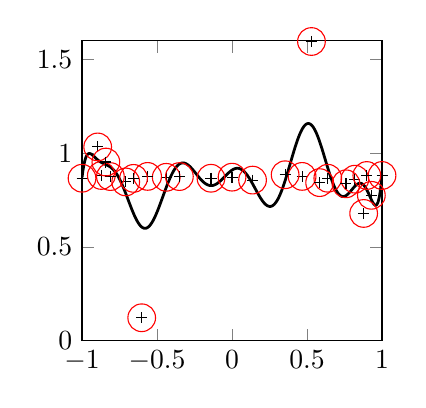
\begin{tikzpicture}

\begin{axis}[%
width=1.5in,
height=1.5in,
scale only axis,
xmin=-1,
xmax=1,
ymin=0,
ymax=1.6,
]
\addplot [color=black,solid,line width=1.0pt,forget plot]
  table[row sep=crcr]{%
-1	0.871080860495567\\
-0.993333333333333	0.911502629518509\\
-0.986666666666667	0.942155033349991\\
-0.98	0.964632302522659\\
-0.973333333333333	0.980349034070969\\
-0.966666666666667	0.990556582808495\\
-0.96	0.9963508695364\\
-0.953333333333333	0.998680248856544\\
-0.946666666666667	0.998367384076118\\
-0.94	0.996106117963791\\
-0.933333333333333	0.992481872439384\\
-0.926666666666667	0.987978920340538\\
-0.92	0.982987523078918\\
-0.913333333333333	0.977815002202988\\
-0.906666666666667	0.972697615623474\\
-0.9	0.96780252456665\\
-0.893333333333333	0.963245391845703\\
-0.886666666666667	0.959086954593658\\
-0.88	0.95534884929657\\
-0.873333333333333	0.952018141746521\\
-0.866666666666667	0.949049085378647\\
-0.86	0.946376800537109\\
-0.853333333333333	0.943917810916901\\
-0.846666666666667	0.941576242446899\\
-0.84	0.9392469227314\\
-0.833333333333333	0.93682137131691\\
-0.826666666666667	0.934192031621933\\
-0.82	0.931251436471939\\
-0.813333333333333	0.92789962887764\\
-0.806666666666667	0.9240443110466\\
-0.8	0.919603675603867\\
-0.793333333333333	0.914504885673523\\
-0.786666666666667	0.908692896366119\\
-0.78	0.902121216058731\\
-0.773333333333333	0.894760251045227\\
-0.766666666666667	0.886597096920013\\
-0.76	0.877629578113556\\
-0.753333333333333	0.867873221635818\\
-0.746666666666667	0.857357293367386\\
-0.74	0.846123650670052\\
-0.733333333333333	0.834228068590164\\
-0.726666666666667	0.821737840771675\\
-0.72	0.808730319142342\\
-0.713333333333333	0.795296087861061\\
-0.706666666666667	0.781528398394585\\
-0.7	0.767531737685204\\
-0.693333333333333	0.753416746854782\\
-0.686666666666667	0.739292293787003\\
-0.68	0.725278481841087\\
-0.673333333333333	0.711488783359528\\
-0.666666666666667	0.698043018579483\\
-0.66	0.685054257512093\\
-0.653333333333333	0.672637715935707\\
-0.646666666666667	0.660898894071579\\
-0.64	0.649943292140961\\
-0.633333333333333	0.639865696430206\\
-0.626666666666667	0.630756840109825\\
-0.62	0.622696757316589\\
-0.613333333333333	0.615755975246429\\
-0.606666666666667	0.609998196363449\\
-0.6	0.605473458766937\\
-0.593333333333333	0.60222239792347\\
-0.586666666666667	0.600273624062538\\
-0.58	0.599646255373955\\
-0.573333333333333	0.600346460938454\\
-0.566666666666667	0.602367475628853\\
-0.56	0.605694100260735\\
-0.553333333333333	0.610296815633774\\
-0.546666666666667	0.616138964891434\\
-0.54	0.623170450329781\\
-0.533333333333333	0.631334185600281\\
-0.526666666666667	0.640562996268272\\
-0.52	0.650778338313103\\
-0.513333333333333	0.661899149417877\\
-0.506666666666667	0.673834100365639\\
-0.5	0.686486691236496\\
-0.493333333333333	0.699757725000381\\
-0.486666666666667	0.713542088866234\\
-0.48	0.727729886770248\\
-0.473333333333333	0.742213517427444\\
-0.466666666666667	0.756881728768349\\
-0.46	0.771623402833939\\
-0.453333333333333	0.786330074071884\\
-0.446666666666667	0.800893738865852\\
-0.44	0.815209925174713\\
-0.433333333333333	0.829179733991623\\
-0.426666666666667	0.84270504117012\\
-0.42	0.855695381760597\\
-0.413333333333333	0.86806845664978\\
-0.406666666666667	0.879745975136757\\
-0.4	0.890659108757973\\
-0.393333333333333	0.900742694735527\\
-0.386666666666667	0.909945920109749\\
-0.38	0.918224185705185\\
-0.373333333333333	0.925541177392006\\
-0.366666666666667	0.931869179010391\\
-0.36	0.937193647027016\\
-0.353333333333333	0.941503748297691\\
-0.346666666666667	0.944800466299057\\
-0.34	0.947096586227417\\
-0.333333333333333	0.948407918214798\\
-0.326666666666667	0.948765575885773\\
-0.32	0.948200985789299\\
-0.313333333333333	0.946759149432182\\
-0.306666666666667	0.94449208676815\\
-0.3	0.941452398896217\\
-0.293333333333333	0.937706157565117\\
-0.286666666666667	0.933319866657257\\
-0.28	0.928366214036942\\
-0.273333333333333	0.922920152544975\\
-0.266666666666667	0.917060032486916\\
-0.26	0.910868540406227\\
-0.253333333333333	0.904427960515022\\
-0.246666666666667	0.897821091115475\\
-0.24	0.891130410134792\\
-0.233333333333333	0.884435974061489\\
-0.226666666666667	0.877819575369358\\
-0.22	0.871357694268227\\
-0.213333333333333	0.865123048424721\\
-0.206666666666667	0.859186753630638\\
-0.2	0.853613950312138\\
-0.193333333333333	0.848463349044323\\
-0.186666666666667	0.843789294362068\\
-0.18	0.839641496539116\\
-0.173333333333333	0.836059704422951\\
-0.166666666666667	0.833075359463692\\
-0.16	0.830720953643322\\
-0.153333333333333	0.829012244939804\\
-0.146666666666667	0.827961318194866\\
-0.14	0.827573850750923\\
-0.133333333333333	0.827842928469181\\
-0.126666666666667	0.82876156270504\\
-0.12	0.830307520925999\\
-0.113333333333333	0.832457154989243\\
-0.106666666666667	0.835175640881062\\
-0.1	0.838425040245056\\
-0.0933333333333333	0.842160582542419\\
-0.0866666666666666	0.846328571438789\\
-0.08	0.85087513178587\\
-0.0733333333333333	0.85573810338974\\
-0.0666666666666667	0.860852085053921\\
-0.0599999999999999	0.866150192916393\\
-0.0533333333333332	0.871560797095299\\
-0.0466666666666666	0.877013586461544\\
-0.0399999999999999	0.882432840764523\\
-0.0333333333333333	0.887744709849358\\
-0.0266666666666666	0.892876751720905\\
-0.0199999999999999	0.897755928337574\\
-0.0133333333333333	0.90231179445982\\
-0.0066666666666666	0.906478516757488\\
0	0.910189259797335\\
0.0066666666666666	0.913385834544897\\
0.0133333333333333	0.916010562330484\\
0.0199999999999999	0.91801467910409\\
0.0266666666666666	0.919353485107422\\
0.0333333333333333	0.919989462941885\\
0.0399999999999999	0.919890467077494\\
0.0466666666666666	0.919034343212843\\
0.0533333333333332	0.91740246117115\\
0.0599999999999999	0.914986532181501\\
0.0666666666666667	0.911790367215872\\
0.0733333333333333	0.907816376537085\\
0.08	0.90308354049921\\
0.0866666666666666	0.897616751492023\\
0.0933333333333333	0.891445942223072\\
0.1	0.884612485766411\\
0.106666666666667	0.877163052558899\\
0.113333333333333	0.869156200438738\\
0.12	0.860649693757296\\
0.126666666666667	0.85171477496624\\
0.133333333333333	0.842425398528576\\
0.14	0.832860797643661\\
0.146666666666667	0.823106683790684\\
0.153333333333333	0.813250411301851\\
0.16	0.803384441882372\\
0.166666666666667	0.793602962046862\\
0.173333333333333	0.784001410007477\\
0.18	0.774678912013769\\
0.186666666666667	0.765729982405901\\
0.193333333333333	0.757250688970089\\
0.2	0.749335628002882\\
0.206666666666667	0.74207784421742\\
0.213333333333333	0.735562892630696\\
0.22	0.729876494035125\\
0.226666666666667	0.725096607580781\\
0.233333333333333	0.721294661983848\\
0.24	0.718539644032717\\
0.246666666666667	0.716888803988695\\
0.253333333333333	0.716390825808048\\
0.26	0.717090347781777\\
0.266666666666667	0.719019865617156\\
0.273333333333333	0.722202422097325\\
0.28	0.726652130484581\\
0.286666666666667	0.732371956110001\\
0.293333333333333	0.739354087039828\\
0.3	0.747583108022809\\
0.306666666666667	0.757028132677078\\
0.313333333333333	0.76765276864171\\
0.32	0.779406264424324\\
0.326666666666667	0.792227491736412\\
0.333333333333333	0.806052768602967\\
0.34	0.820799851790071\\
0.346666666666667	0.836381698958576\\
0.353333333333333	0.852702875621617\\
0.36	0.869661035016179\\
0.366666666666667	0.887145509943366\\
0.373333333333333	0.905039585195482\\
0.38	0.923223889432847\\
0.386666666666667	0.941570690833032\\
0.393333333333333	0.959950605407357\\
0.4	0.97823385708034\\
0.406666666666667	0.996289753355086\\
0.413333333333333	1.013980303891\\
0.42	1.0311810048297\\
0.426666666666667	1.04775645956397\\
0.433333333333333	1.06358524225652\\
0.44	1.07854454126209\\
0.446666666666667	1.09251660481095\\
0.453333333333333	1.10539527703077\\
0.46	1.11707504559308\\
0.466666666666667	1.12746537663043\\
0.473333333333333	1.13647929020226\\
0.48	1.14404658041894\\
0.486666666666667	1.15010186750442\\
0.493333333333333	1.15459522744641\\
0.5	1.15748983668163\\
0.506666666666667	1.15875590825453\\
0.513333333333333	1.15838513476774\\
0.52	1.15637653833255\\
0.526666666666667	1.15274527110159\\
0.533333333333333	1.14752023573965\\
0.54	1.14074295014143\\
0.546666666666667	1.13246828131378\\
0.553333333333333	1.12276478391141\\
0.56	1.11171564180404\\
0.566666666666667	1.09941092459485\\
0.573333333333333	1.08595735626295\\
0.58	1.07146791135892\\
0.586666666666667	1.05606869980693\\
0.593333333333333	1.0398910632357\\
0.6	1.02307299943641\\
0.606666666666667	1.00576433446258\\
0.613333333333333	0.988112322287634\\
0.62	0.970271246973425\\
0.626666666666667	0.952398091787472\\
0.633333333333333	0.934646362205967\\
0.64	0.917167344130576\\
0.646666666666667	0.900116100674495\\
0.653333333333333	0.883634599624202\\
0.66	0.867865458829328\\
0.666666666666667	0.852937435498461\\
0.673333333333333	0.83897241554223\\
0.68	0.826080629369244\\
0.686666666666667	0.814359018811956\\
0.693333333333333	0.803892683237791\\
0.7	0.79474739311263\\
0.706666666666667	0.78697609109804\\
0.713333333333333	0.780612038681284\\
0.72	0.775671270559542\\
0.726666666666667	0.772151695215143\\
0.733333333333333	0.770026609883644\\
0.74	0.769256696337834\\
0.746666666666667	0.76977717585396\\
0.753333333333333	0.771506590070203\\
0.76	0.774344218429178\\
0.766666666666667	0.77817104884889\\
0.773333333333333	0.782848771777935\\
0.78	0.788225708296522\\
0.786666666666667	0.794133519404568\\
0.793333333333333	0.800392117584124\\
0.8	0.806813869741745\\
0.806666666666667	0.813201332115568\\
0.813333333333333	0.819351937971078\\
0.82	0.825063803815283\\
0.826666666666667	0.830138723133132\\
0.833333333333333	0.83437842753483\\
0.84	0.837607907014899\\
0.846666666666667	0.839651910820976\\
0.853333333333333	0.840369191719219\\
0.86	0.839634875650518\\
0.866666666666667	0.837361696409062\\
0.873333333333333	0.833497695683036\\
0.88	0.828032078105025\\
0.886666666666667	0.821004733617883\\
0.893333333333333	0.812513404875062\\
0.9	0.802719077037182\\
0.906666666666667	0.791851329617202\\
0.913333333333333	0.780216799757909\\
0.92	0.76820944721112\\
0.926666666666667	0.756314025842585\\
0.933333333333333	0.745112903183326\\
0.94	0.735300561675103\\
0.946666666666667	0.727681809483329\\
0.953333333333333	0.723186431045178\\
0.96	0.722874706989387\\
0.966666666666667	0.727942201192491\\
0.973333333333333	0.739730050147045\\
0.98	0.759731092053698\\
0.986666666666667	0.789598370873136\\
0.993333333333333	0.831147338292794\\
1	0.886367861414328\\
};
\addplot [color=black,only marks,mark=+,mark options={solid},forget plot]
  table[row sep=crcr]{%
0.818827708703375	0.861888122983872\\
};
\addplot [color=red,mark size=5.0pt,only marks,mark=o,mark options={solid},forget plot]
  table[row sep=crcr]{%
0.818827708703375	0.861888122983872\\
};
\addplot [color=black,only marks,mark=+,mark options={solid},forget plot]
  table[row sep=crcr]{%
0.136767317939609	0.856960457661291\\
};
\addplot [color=red,mark size=5.0pt,only marks,mark=o,mark options={solid},forget plot]
  table[row sep=crcr]{%
0.136767317939609	0.856960457661291\\
};
\addplot [color=black,only marks,mark=+,mark options={solid},forget plot]
  table[row sep=crcr]{%
-0.438721136767318	0.871743453629032\\
};
\addplot [color=red,mark size=5.0pt,only marks,mark=o,mark options={solid},forget plot]
  table[row sep=crcr]{%
-0.438721136767318	0.871743453629032\\
};
\addplot [color=black,only marks,mark=+,mark options={solid},forget plot]
  table[row sep=crcr]{%
-1	0.866815788306452\\
};
\addplot [color=red,mark size=5.0pt,only marks,mark=o,mark options={solid},forget plot]
  table[row sep=crcr]{%
-1	0.866815788306452\\
};
\addplot [color=black,only marks,mark=+,mark options={solid},forget plot]
  table[row sep=crcr]{%
-0.708703374777975	0.847105127016129\\
};
\addplot [color=red,mark size=5.0pt,only marks,mark=o,mark options={solid},forget plot]
  table[row sep=crcr]{%
-0.708703374777975	0.847105127016129\\
};
\addplot [color=black,only marks,mark=+,mark options={solid},forget plot]
  table[row sep=crcr]{%
-0.140319715808171	0.866815788306452\\
};
\addplot [color=red,mark size=5.0pt,only marks,mark=o,mark options={solid},forget plot]
  table[row sep=crcr]{%
-0.140319715808171	0.866815788306452\\
};
\addplot [color=black,only marks,mark=+,mark options={solid},forget plot]
  table[row sep=crcr]{%
0.467140319715808	0.876671118951613\\
};
\addplot [color=red,mark size=5.0pt,only marks,mark=o,mark options={solid},forget plot]
  table[row sep=crcr]{%
0.467140319715808	0.876671118951613\\
};
\addplot [color=black,only marks,mark=+,mark options={solid},forget plot]
  table[row sep=crcr]{%
1	0.881598784274194\\
};
\addplot [color=red,mark size=5.0pt,only marks,mark=o,mark options={solid},forget plot]
  table[row sep=crcr]{%
1	0.881598784274194\\
};
\addplot [color=black,only marks,mark=+,mark options={solid},forget plot]
  table[row sep=crcr]{%
0.529500756429652	1.59611025604839\\
};
\addplot [color=red,mark size=5.0pt,only marks,mark=o,mark options={solid},forget plot]
  table[row sep=crcr]{%
0.529500756429652	1.59611025604839\\
};
\addplot [color=black,only marks,mark=+,mark options={solid},forget plot]
  table[row sep=crcr]{%
-0.602118003025719	0.122738324596774\\
};
\addplot [color=red,mark size=5.0pt,only marks,mark=o,mark options={solid},forget plot]
  table[row sep=crcr]{%
-0.602118003025719	0.122738324596774\\
};
\addplot [color=black,only marks,mark=+,mark options={solid},forget plot]
  table[row sep=crcr]{%
0.638426626323752	0.866815788306452\\
};
\addplot [color=red,mark size=5.0pt,only marks,mark=o,mark options={solid},forget plot]
  table[row sep=crcr]{%
0.638426626323752	0.866815788306452\\
};
\addplot [color=black,only marks,mark=+,mark options={solid},forget plot]
  table[row sep=crcr]{%
-0.871406959152799	0.881598784274194\\
};
\addplot [color=red,mark size=5.0pt,only marks,mark=o,mark options={solid},forget plot]
  table[row sep=crcr]{%
-0.871406959152799	0.881598784274194\\
};
\addplot [color=black,only marks,mark=+,mark options={solid},forget plot]
  table[row sep=crcr]{%
-0.562783661119516	0.876671118951613\\
};
\addplot [color=red,mark size=5.0pt,only marks,mark=o,mark options={solid},forget plot]
  table[row sep=crcr]{%
-0.562783661119516	0.876671118951613\\
};
\addplot [color=black,only marks,mark=+,mark options={solid},forget plot]
  table[row sep=crcr]{%
0.898638426626323	0.881598784274194\\
};
\addplot [color=red,mark size=5.0pt,only marks,mark=o,mark options={solid},forget plot]
  table[row sep=crcr]{%
0.898638426626323	0.881598784274194\\
};
\addplot [color=black,only marks,mark=+,mark options={solid},forget plot]
  table[row sep=crcr]{%
0.75945537065053	0.837096774193548\\
};
\addplot [color=red,mark size=5.0pt,only marks,mark=o,mark options={solid},forget plot]
  table[row sep=crcr]{%
0.75945537065053	0.837096774193548\\
};
\addplot [color=black,only marks,mark=+,mark options={solid},forget plot]
  table[row sep=crcr]{%
-0.81089258698941	0.875806451612903\\
};
\addplot [color=red,mark size=5.0pt,only marks,mark=o,mark options={solid},forget plot]
  table[row sep=crcr]{%
-0.81089258698941	0.875806451612903\\
};
\addplot [color=black,only marks,mark=+,mark options={solid},forget plot]
  table[row sep=crcr]{%
0.583963691376702	0.843548387096774\\
};
\addplot [color=red,mark size=5.0pt,only marks,mark=o,mark options={solid},forget plot]
  table[row sep=crcr]{%
0.583963691376702	0.843548387096774\\
};
\addplot [color=black,only marks,mark=+,mark options={solid},forget plot]
  table[row sep=crcr]{%
-0.656580937972769	0.866129032258065\\
};
\addplot [color=red,mark size=5.0pt,only marks,mark=o,mark options={solid},forget plot]
  table[row sep=crcr]{%
-0.656580937972769	0.866129032258065\\
};
\addplot [color=black,only marks,mark=+,mark options={solid},forget plot]
  table[row sep=crcr]{%
-0.350983358547655	0.875806451612903\\
};
\addplot [color=red,mark size=5.0pt,only marks,mark=o,mark options={solid},forget plot]
  table[row sep=crcr]{%
-0.350983358547655	0.875806451612903\\
};
\addplot [color=black,only marks,mark=+,mark options={solid},forget plot]
  table[row sep=crcr]{%
0	0.87258064516129\\
};
\addplot [color=red,mark size=5.0pt,only marks,mark=o,mark options={solid},forget plot]
  table[row sep=crcr]{%
0	0.87258064516129\\
};
\addplot [color=black,only marks,mark=+,mark options={solid},forget plot]
  table[row sep=crcr]{%
0.354009077155824	0.885483870967742\\
};
\addplot [color=red,mark size=5.0pt,only marks,mark=o,mark options={solid},forget plot]
  table[row sep=crcr]{%
0.354009077155824	0.885483870967742\\
};
\addplot [color=black,only marks,mark=+,mark options={solid},forget plot]
  table[row sep=crcr]{%
0.877458396369138	0.679032258064516\\
};
\addplot [color=red,mark size=5.0pt,only marks,mark=o,mark options={solid},forget plot]
  table[row sep=crcr]{%
0.877458396369138	0.679032258064516\\
};
\addplot [color=black,only marks,mark=+,mark options={solid},forget plot]
  table[row sep=crcr]{%
-0.895612708018154	1.03387096774194\\
};
\addplot [color=red,mark size=5.0pt,only marks,mark=o,mark options={solid},forget plot]
  table[row sep=crcr]{%
-0.895612708018154	1.03387096774194\\
};
\addplot [color=black,only marks,mark=+,mark options={solid},forget plot]
  table[row sep=crcr]{%
0.928895612708018	0.775806451612903\\
};
\addplot [color=red,mark size=5.0pt,only marks,mark=o,mark options={solid},forget plot]
  table[row sep=crcr]{%
0.928895612708018	0.775806451612903\\
};
\addplot [color=black,only marks,mark=+,mark options={solid},forget plot]
  table[row sep=crcr]{%
-0.841149773071104	0.953225806451613\\
};
\addplot [color=red,mark size=5.0pt,only marks,mark=o,mark options={solid},forget plot]
  table[row sep=crcr]{%
-0.841149773071104	0.953225806451613\\
};
\end{axis}
\end{tikzpicture}%
\end{document}
\caption{On this data set the linear kernel is able to outperform a radial basis function kernel, which is more susceptible to the noisy outliers.}
\label{fig:linearKing}
\end{figure}
Figure~\ref{fig:linearKing} shows an example of an approximately line-like function with some outliers. In this case a simple linear kernel is a good choice, as it is unable to track the added complexity of the noise. An rbf-function kernel is able to integrate the noise into the model, but in this example one would like to avoid this. However it is possible to fundamentally improve the rbf kernel results if changes the parameters $\sigma, c$\footnote{$c$ is the regularization parameter. It is called $\gamma$ in svm toolbox functions.} and $\epsilon$ are changed more towards regularization. Most notably the parameter $c$, which determines the tolerance for deviation from the desired $\epsilon$-accuracy can be used to improve the performance of the rbf-kernel. If $c$ is set to a comparatively large value with $\epsilon$ kept small results improve. A good choice will use a moderate value for $\epsilon$ to reduce the amount of support vectors and thereby increases the sparsity of the solution vector\footnote{Support Vector Machines: Methods and Applications, Suykens et al., page 33}, while using $c$ to make sure the solution is not to prone to deviations introduced by outliers.
 
\subsection{Sum of cosines}
As an initial example noise free function:
\begin{equation}
f(x) = \cos(x) + \cos(2x)
\end{equation}
will be considered. Finding a good set of hyper-parameters by hand can be tricky as figure~\ref{fig:estParamsTricky} illustrates. Where for it can be noticed that the approximation tends to oscillate if $\sigma^2$ is chosen very small. This can be explained using equation~\ref{eq:Ksum}, which states that the estimator is created by superposing weighted and shifted the kernel functions. In this case Gaussians are added up. If their width ($\sigma^2$) becomes small their sum must oscillate, because the Gaussians will not overlap sufficiently. The height of the gaussians is controlled by the regularization parameter $\gamma$, as it acts like a box constraint when the dual is formed. Thus, when $\gamma$ is chosen too small the kernel functions can not be tall enough to approximate the function.  
To make a good choice a hundred by hundred grid in $\sigma^2 \in [10^{-5},10^{0}]$ and $\gamma \in [10^{0},10^{10}]$  has been searched using the two norm of the error vector $(\mathbf{y}_{est} - \mathbf{y})$ as cost function. The error function on the described input space as well as the estimator with the lowest error is shown in figure~\ref{fig:cosEst}. The grid search led to optimal the parameter pair $\sigma^2 = 0.0019$ and $\gamma = 10.2353$. Estimation results are shown in the middle of figure~\ref{fig:cosEst} training set performance is plotted on the left.
Next a noisy version of $f(x)$ is considered:
\begin{equation}
f(x)_n = \cos(x) + \cos(2x) + x_n
\end{equation}
With the values for $x_n$ drawn from the normal distribution $\mathcal{N}(0,0.1^2)$. The changed situation is shown in figure~\ref{fig:cosEstNoise}. When noise is added on average the optimal values for $\sigma^2$ must be chosen larger to avoid 
over-fitting.
\begin{figure}
\centering
% This file was created by matlab2tikz.
% Minimal pgfplots version: 1.3
%
%The latest updates can be retrieved from
%  http://www.mathworks.com/matlabcentral/fileexchange/22022-matlab2tikz
%where you can also make suggestions and rate matlab2tikz.
%
\documentclass[tikz]{standalone}
\usepackage{pgfplots}
\usepackage{grffile}
\pgfplotsset{compat=newest}
\usetikzlibrary{plotmarks}
\usepackage{amsmath}

\begin{document}
\definecolor{mycolor1}{rgb}{0.00000,0.44700,0.74100}%
\definecolor{mycolor2}{rgb}{0.85000,0.32500,0.09800}%
\definecolor{mycolor3}{rgb}{0.92900,0.69400,0.12500}%
\definecolor{mycolor4}{rgb}{0.49400,0.18400,0.55600}%
\definecolor{mycolor5}{rgb}{0.46600,0.67400,0.18800}%
\definecolor{mycolor6}{rgb}{0.30100,0.74500,0.93300}%
\definecolor{mycolor7}{rgb}{0.63500,0.07800,0.18400}%
%
\begin{tikzpicture}

\begin{axis}[%
width=4.5in,
height=1.5in,
at={(1.365in,0.503021in)},
scale only axis,
xmin=-10,
xmax=10,
ymin=-1.5,
ymax=2.5
]
\addplot [color=mycolor1,solid,forget plot]
  table[row sep=crcr]{%
-10	-0.453244582719315\\
-9.99	-0.455212941236136\\
-9.98	-0.457155926566137\\
-9.97	-0.45907318552017\\
-9.96	-0.460964365809557\\
-9.95	-0.46282911609962\\
-9.94	-0.464667086063343\\
-9.93	-0.466477926435328\\
-9.92	-0.468261289065744\\
-9.91	-0.470016826974587\\
-9.9	-0.471744194406018\\
-9.89	-0.473443046882807\\
-9.88	-0.475113041261005\\
-9.87	-0.47675383578463\\
-9.86	-0.478365090140567\\
-9.85	-0.479946465513495\\
-9.84	-0.481497624640938\\
-9.83	-0.483018231868444\\
-9.82	-0.48450795320478\\
-9.81	-0.485966456377224\\
-9.8	-0.487393410886948\\
-9.79	-0.488788488064396\\
-9.78	-0.49015136112475\\
-9.77	-0.491481705223432\\
-9.76	-0.492779197511575\\
-9.75	-0.494043517191614\\
-9.74	-0.495274345572773\\
-9.73	-0.496471366126601\\
-9.72	-0.497634264542543\\
-9.71	-0.498762728783368\\
-9.7	-0.499856449140706\\
-9.69	-0.500915118290448\\
-9.68	-0.501938431348141\\
-9.67	-0.502926085924273\\
-9.66	-0.503877782179596\\
-9.65	-0.504793222880245\\
-9.64	-0.505672113452835\\
-9.63	-0.506514162039485\\
-9.62	-0.507319079552652\\
-9.61	-0.508086579729934\\
-9.6	-0.508816379188685\\
-9.59	-0.509508197480547\\
-9.58	-0.510161757145742\\
-9.57	-0.510776783767344\\
-9.56	-0.511353006025262\\
-9.55	-0.511890155750097\\
-9.54	-0.512387967976836\\
-9.53	-0.512846180998283\\
-9.52	-0.513264536418354\\
-9.51	-0.513642779205116\\
-9.5	-0.513980657743584\\
-9.49	-0.514277923888349\\
-9.48	-0.514534333015874\\
-9.47	-0.514749644076581\\
-9.46	-0.514923619646685\\
-9.45	-0.515056025979705\\
-9.44	-0.515146633057711\\
-9.43	-0.515195214642328\\
-9.42	-0.515201548325261\\
-9.41	-0.515165415578779\\
-9.4	-0.515086601805569\\
-9.39	-0.514964896388521\\
-9.38	-0.514800092739934\\
-9.37	-0.51459198835055\\
-9.36	-0.514340384838125\\
-9.35	-0.514045087995611\\
-9.34	-0.513705907839044\\
-9.33	-0.513322658654905\\
-9.32	-0.512895159047192\\
-9.31	-0.512423231984015\\
-9.3	-0.511906704843757\\
-9.29	-0.511345409460846\\
-9.28	-0.510739182171019\\
-9.27	-0.510087863856197\\
-9.26	-0.509391299988831\\
-9.25	-0.508649340675827\\
-9.24	-0.507861840701974\\
-9.23	-0.507028659572789\\
-9.22	-0.506149661557045\\
-9.21	-0.505224715728598\\
-9.2	-0.504253696007808\\
-9.19	-0.503236481202346\\
-9.18	-0.502172955047572\\
-9.17	-0.501063006246233\\
-9.16	-0.499906528507701\\
-9.15	-0.498703420586571\\
-9.14	-0.497453586320755\\
-9.13	-0.496156934668916\\
-9.12	-0.49481337974734\\
-9.11	-0.493422840866232\\
-9.1	-0.491985242565336\\
-9.09	-0.49050051464899\\
-9.08	-0.488968592220513\\
-9.07	-0.487389415715951\\
-9.06	-0.485762930937272\\
-9.05	-0.484089089084703\\
-9.04	-0.482367846788628\\
-9.03	-0.48059916614064\\
-9.02	-0.478783014724053\\
-9.01	-0.476919365643561\\
-9	-0.475008197554401\\
-8.99	-0.473049494690616\\
-8.98	-0.471043246892759\\
-8.97	-0.46898944963479\\
-8.96	-0.466888104050256\\
-8.95	-0.464739216957765\\
-8.94	-0.462542800885724\\
-8.93	-0.460298874096263\\
-8.92	-0.458007460608494\\
-8.91	-0.455668590220911\\
-8.9	-0.453282298533146\\
-8.89	-0.450848626966769\\
-8.88	-0.448367622785492\\
-8.87	-0.445839339114469\\
-8.86	-0.443263834958798\\
-8.85	-0.440641175221318\\
-8.84	-0.437971430719458\\
-8.83	-0.435254678201411\\
-8.82	-0.432491000361337\\
-8.81	-0.429680485853909\\
-8.8	-0.426823229307891\\
-8.79	-0.42391933133891\\
-8.78	-0.420968898561427\\
-8.77	-0.417972043599869\\
-8.76	-0.41492888509878\\
-8.75	-0.411839547732267\\
-8.74	-0.408704162212528\\
-8.73	-0.405522865297455\\
-8.72	-0.402295799797461\\
-8.71	-0.399023114581341\\
-8.7	-0.395704964581325\\
-8.69	-0.392341510797194\\
-8.68	-0.388932920299501\\
-8.67	-0.385479366231973\\
-8.66	-0.381981027812925\\
-8.65	-0.378438090335813\\
-8.64	-0.374850745168892\\
-8.63	-0.371219189753964\\
-8.62	-0.367543627604186\\
-8.61	-0.363824268300984\\
-8.6	-0.360061327490068\\
-8.59	-0.356255026876522\\
-8.58	-0.352405594218919\\
-8.57	-0.348513263322589\\
-8.56	-0.344578274031928\\
-8.55	-0.340600872221749\\
-8.54	-0.336581309787774\\
-8.53	-0.332519844636115\\
-8.52	-0.328416740671879\\
-8.51	-0.324272267786815\\
-8.5	-0.320086701846043\\
-8.49	-0.315860324673797\\
-8.48	-0.311593424038312\\
-8.47	-0.307286293635704\\
-8.46	-0.302939233072932\\
-8.45	-0.298552547849838\\
-8.44	-0.294126549340229\\
-8.43	-0.289661554772028\\
-8.42	-0.285157887206484\\
-8.41	-0.280615875516431\\
-8.4	-0.276035854363653\\
-8.39	-0.271418164175239\\
-8.38	-0.266763151119085\\
-8.37	-0.26207116707839\\
-8.36	-0.257342569625269\\
-8.35	-0.252577721993376\\
-8.34	-0.247776993049671\\
-8.33	-0.242940757265195\\
-8.32	-0.238069394684958\\
-8.31	-0.233163290896846\\
-8.3	-0.228222836999696\\
-8.29	-0.223248429570355\\
-8.28	-0.218240470629881\\
-8.27	-0.213199367608791\\
-8.26	-0.208125533311453\\
-8.25	-0.203019385879483\\
-8.24	-0.197881348754341\\
-8.23	-0.19271185063891\\
-8.22	-0.187511325458269\\
-8.21	-0.182280212319524\\
-8.2	-0.177018955470772\\
-8.19	-0.171728004259135\\
-8.18	-0.166407813087986\\
-8.17	-0.161058841373208\\
-8.16	-0.155681553498649\\
-8.15	-0.150276418770682\\
-8.14	-0.144843911371891\\
-8.13	-0.139384510313917\\
-8.12	-0.133898699389445\\
-8.11	-0.128386967123344\\
-8.1	-0.122849806722942\\
-8.09	-0.117287716027523\\
-8.08	-0.111701197456914\\
-8.07	-0.106090757959313\\
-8.06	-0.100456908958282\\
-8.05	-0.0948001662989022\\
-8.04	-0.0891210501931672\\
-8.03	-0.0834200851645403\\
-8.02	-0.0776977999917398\\
-8.01	-0.0719547276517451\\
-8	-0.0661914052620092\\
-7.99	-0.0604083740219119\\
-7.98	-0.0546061791534809\\
-7.97	-0.0487853698412659\\
-7.96	-0.0429464991716025\\
-7.95	-0.0370901240710177\\
-7.94	-0.0312168052439783\\
-7.93	-0.0253271071098803\\
-7.92	-0.0194215977393461\\
-7.91	-0.013500848789817\\
-7.9	-0.00756543544043406\\
-7.89	-0.00161593632626027\\
-7.88	0.00434706652822901\\
-7.87	0.0103229877762366\\
-7.86	0.016311238816487\\
-7.85	0.022311227861642\\
-7.84	0.0283223600074152\\
-7.83	0.0343440373022703\\
-7.82	0.0403756588177775\\
-7.81	0.0464166207195435\\
-7.8	0.0524663163387809\\
-7.79	0.0585241362444242\\
-7.78	0.0645894683158667\\
-7.77	0.0706616978162352\\
-7.76	0.0767402074662432\\
-7.75	0.0828243775185866\\
-7.74	0.0889135858328507\\
-7.73	0.0950072079509799\\
-7.72	0.101104617173274\\
-7.71	0.107205184634801\\
-7.7	0.113308279382423\\
-7.69	0.119413268452191\\
-7.68	0.125519516947301\\
-7.67	0.131626388116443\\
-7.66	0.137733243432619\\
-7.65	0.143839442672412\\
-7.64	0.149944343995647\\
-7.63	0.156047304025479\\
-7.62	0.162147677928871\\
-7.61	0.16824481949747\\
-7.6	0.174338081228852\\
-7.59	0.180426814408111\\
-7.58	0.186510369189844\\
-7.57	0.192588094680386\\
-7.56	0.19865933902049\\
-7.55	0.204723449468182\\
-7.54	0.210779772482041\\
-7.53	0.216827653804675\\
-7.52	0.222866438546513\\
-7.51	0.228895471269837\\
-7.5	0.234914096073085\\
-7.49	0.240921656675372\\
-7.48	0.246917496501194\\
-7.47	0.25290095876544\\
-7.46	0.258871386558485\\
-7.45	0.264828122931548\\
-7.44	0.270770510982156\\
-7.43	0.276697893939817\\
-7.42	0.282609615251797\\
-7.41	0.288505018669034\\
-7.4	0.294383448332176\\
-7.39	0.300244248857709\\
-7.38	0.306086765424173\\
-7.37	0.311910343858446\\
-7.36	0.317714330722117\\
-7.35	0.323498073397861\\
-7.34	0.329260920175891\\
-7.33	0.33500222034039\\
-7.32	0.340721324255964\\
-7.31	0.346417583454117\\
-7.3	0.352090350719648\\
-7.29	0.35773898017705\\
-7.28	0.363362827376845\\
-7.27	0.36896124938188\\
-7.26	0.374533604853506\\
-7.25	0.380079254137687\\
-7.24	0.385597559351035\\
-7.23	0.391087884466669\\
-7.22	0.396549595399989\\
-7.21	0.401982060094261\\
-7.2	0.40738464860612\\
-7.19	0.412756733190796\\
-7.18	0.418097688387256\\
-7.17	0.423406891103061\\
-7.16	0.428683720699074\\
-7.15	0.433927559073922\\
-7.14	0.439137790748183\\
-7.13	0.444313802948376\\
-7.12	0.449454985690635\\
-7.11	0.454560731864161\\
-7.1	0.4596304373143\\
-7.09	0.464663500925396\\
-7.08	0.469659324703258\\
-7.07	0.474617313857353\\
-7.06	0.479536876882606\\
-7.05	0.484417425640856\\
-7.04	0.489258375441938\\
-7.03	0.494059145124411\\
-7.02	0.498819157135835\\
-7.01	0.503537837612652\\
-7	0.508214616459703\\
-6.99	0.512848927429204\\
-6.98	0.517440208199361\\
-6.97	0.521987900452492\\
-6.96	0.526491449952663\\
-6.95	0.530950306622862\\
-6.94	0.535363924621648\\
-6.93	0.539731762419322\\
-6.92	0.544053282873551\\
-6.91	0.548327953304452\\
-6.9	0.552555245569176\\
-6.89	0.556734636135851\\
-6.88	0.560865606157058\\
-6.87	0.56494764154262\\
-6.86	0.568980233031875\\
-6.85	0.572962876265332\\
-6.84	0.576895071855672\\
-6.83	0.580776325458154\\
-6.82	0.584606147840374\\
-6.81	0.588384054951402\\
-6.8	0.592109567990204\\
-6.79	0.595782213473439\\
-6.78	0.599401523302553\\
-6.77	0.602967034830201\\
-6.76	0.60647829092593\\
-6.75	0.609934840041207\\
-6.74	0.613336236273657\\
-6.73	0.61668203943063\\
-6.72	0.61997181509198\\
-6.71	0.623205134672106\\
-6.7	0.626381575481278\\
-6.69	0.629500720786083\\
-6.68	0.632562159869217\\
-6.67	0.635565488088389\\
-6.66	0.63851030693448\\
-6.65	0.641396224088889\\
-6.64	0.644222853480021\\
-6.63	0.646989815339015\\
-6.62	0.649696736254592\\
-6.61	0.652343249227071\\
-6.6	0.65492899372154\\
-6.59	0.657453615720186\\
-6.58	0.659916767773711\\
-6.57	0.662318109051912\\
-6.56	0.664657305393408\\
-6.55	0.66693402935439\\
-6.54	0.669147960256574\\
-6.53	0.67129878423416\\
-6.52	0.673386194279971\\
-6.51	0.675409890290603\\
-6.5	0.677369579110703\\
-6.49	0.679264974576262\\
-6.48	0.681095797557032\\
-6.47	0.682861775997972\\
-6.46	0.684562644959734\\
-6.45	0.686198146658224\\
-6.44	0.687768030503174\\
-6.43	0.689272053135786\\
-6.42	0.690709978465354\\
-6.41	0.692081577704969\\
-6.4	0.693386629406214\\
-6.39	0.694624919492844\\
-6.38	0.695796241293559\\
-6.37	0.696900395573693\\
-6.36	0.697937190565968\\
-6.35	0.698906442000201\\
-6.34	0.69980797313205\\
-6.33	0.700641614770719\\
-6.32	0.701407205305651\\
-6.31	0.702104590732216\\
-6.3	0.702733624676375\\
-6.29	0.703294168418321\\
-6.28	0.703786090915075\\
-6.27	0.704209268822111\\
-6.26	0.704563586513865\\
-6.25	0.704848936103302\\
-6.24	0.705065217460347\\
-6.23	0.705212338229382\\
-6.22	0.705290213845641\\
-6.21	0.705298767550552\\
-6.2	0.705237930406105\\
-6.19	0.705107641308093\\
-6.18	0.70490784699838\\
-6.17	0.704638502076077\\
-6.16	0.704299569007687\\
-6.15	0.70389101813621\\
-6.14	0.703412827689173\\
-6.13	0.702864983785676\\
-6.12	0.702247480442287\\
-6.11	0.701560319578\\
-6.1	0.700803511018073\\
-6.09	0.699977072496831\\
-6.08	0.699081029659457\\
-6.07	0.698115416062707\\
-6.06	0.697080273174552\\
-6.05	0.695975650372855\\
-6.04	0.694801604942961\\
-6.03	0.6935582020742\\
-6.02	0.692245514855462\\
-6.01	0.690863624269619\\
-6	0.689412619186994\\
-5.99	0.687892596357747\\
-5.98	0.686303660403282\\
-5.97	0.684645923806558\\
-5.96	0.682919506901422\\
-5.95	0.681124537860929\\
-5.94	0.679261152684572\\
-5.93	0.67732949518461\\
-5.92	0.675329716971258\\
-5.91	0.673261977436945\\
-5.9	0.671126443739562\\
-5.89	0.668923290784659\\
-5.88	0.666652701206703\\
-5.87	0.664314865349295\\
-5.86	0.661909981244416\\
-5.85	0.659438254590695\\
-5.84	0.656899898730671\\
-5.83	0.654295134627092\\
-5.82	0.65162419083825\\
-5.81	0.648887303492325\\
-5.8	0.646084716260804\\
-5.79	0.643216680330875\\
-5.78	0.640283454376959\\
-5.77	0.637285304531218\\
-5.76	0.634222504353173\\
-5.75	0.631095334798334\\
-5.74	0.627904084185977\\
-5.73	0.624649048165934\\
-5.72	0.621330529684443\\
-5.71	0.617948838949206\\
-5.7	0.614504293393417\\
-5.69	0.610997217638931\\
-5.68	0.607427943458593\\
-5.67	0.603796809737593\\
-5.66	0.600104162434026\\
-5.65	0.596350354538521\\
-5.64	0.592535746033056\\
-5.63	0.58866070384884\\
-5.62	0.584725601823459\\
-5.61	0.580730820657074\\
-5.6	0.576676747867838\\
-5.59	0.572563777746489\\
-5.58	0.568392311310091\\
-5.57	0.564162756254988\\
-5.56	0.559875526908986\\
-5.55	0.555531044182633\\
-5.54	0.551129735519858\\
-5.53	0.546672034847715\\
-5.52	0.542158382525413\\
-5.51	0.537589225292564\\
-5.5	0.532965016216689\\
-5.49	0.528286214639977\\
-5.48	0.523553286125294\\
-5.47	0.518766702401492\\
-5.46	0.513926941307967\\
-5.45	0.509034486738535\\
-5.44	0.504089828584598\\
-5.43	0.499093462677608\\
-5.42	0.49404589073087\\
-5.41	0.488947620280644\\
-5.4	0.483799164626625\\
-5.39	0.478601042771712\\
-5.38	0.473353779361195\\
-5.37	0.468057904621247\\
-5.36	0.462713954296844\\
-5.35	0.457322469589023\\
-5.34	0.451883997091566\\
-5.33	0.446399088727065\\
-5.32	0.440868301682422\\
-5.31	0.435292198343754\\
-5.3	0.429671346230731\\
-5.29	0.424006317930369\\
-5.28	0.418297691030272\\
-5.27	0.412546048051321\\
-5.26	0.406751976379858\\
-5.25	0.400916068199339\\
-5.24	0.395038920421491\\
-5.23	0.389121134616938\\
-5.22	0.383163316945412\\
-5.21	0.377166078085398\\
-5.2	0.371130033163378\\
-5.19	0.365055801682599\\
-5.18	0.358944007451386\\
-5.17	0.352795278511022\\
-5.16	0.346610247063233\\
-5.15	0.340389549397203\\
-5.14	0.334133825816229\\
-5.13	0.327843720563971\\
-5.12	0.321519881750309\\
-5.11	0.315162961276833\\
-5.1	0.308773614761974\\
-5.09	0.302352501465772\\
-5.08	0.295900284214312\\
-5.07	0.289417629323829\\
-5.06	0.282905206524481\\
-5.05	0.276363688883822\\
-5.04	0.269793752729973\\
-5.03	0.263196077574484\\
-5.02	0.256571346034962\\
-5.01	0.249920243757375\\
-5	0.243243459338138\\
-4.99	0.236541684245932\\
-4.98	0.229815612743286\\
-4.97	0.223065941807948\\
-4.96	0.216293371053999\\
-4.95	0.209498602652816\\
-4.94	0.202682341253792\\
-4.93	0.195845293904885\\
-4.92	0.188988169973003\\
-4.91	0.182111681064204\\
-4.9	0.17521654094375\\
-4.89	0.168303465456013\\
-4.88	0.161373172444259\\
-4.87	0.154426381670269\\
-4.86	0.147463814733894\\
-4.85	0.140486194992472\\
-4.84	0.133494247480158\\
-4.83	0.126488698827169\\
-4.82	0.119470277178958\\
-4.81	0.112439712115317\\
-4.8	0.10539773456943\\
-4.79	0.0983450767468576\\
-4.78	0.0912824720445469\\
-4.77	0.0842106549697214\\
-4.76	0.0771303610588455\\
-4.75	0.0700423267965246\\
-4.74	0.0629472895344278\\
-4.73	0.0558459874102229\\
-4.72	0.0487391592665302\\
-4.71	0.0416275445699079\\
-4.7	0.034511883329878\\
-4.69	0.0273929160179972\\
-4.68	0.0202713834870078\\
-4.67	0.0131480268900166\\
-4.66	0.00602358759978906\\
-4.65	-0.00110119287188569\\
-4.64	-0.00822557295473024\\
-4.63	-0.0153488111004213\\
-4.62	-0.0224701658629054\\
-4.61	-0.0295888959785927\\
-4.6	-0.0367042604464356\\
-4.59	-0.0438155186078447\\
-4.58	-0.0509219302264753\\
-4.57	-0.0580227555678546\\
-4.56	-0.0651172554788256\\
-4.55	-0.0722046914668464\\
-4.54	-0.0792843257790769\\
-4.53	-0.086355421481304\\
-4.52	-0.0934172425366437\\
-4.51	-0.100469053884055\\
-4.5	-0.107510121516622\\
-4.49	-0.114539712559624\\
-4.48	-0.121557095348385\\
-4.47	-0.128561539505844\\
-4.46	-0.135552316019938\\
-4.45	-0.142528697320675\\
-4.44	-0.149489957356979\\
-4.43	-0.156435371673259\\
-4.42	-0.163364217485686\\
-4.41	-0.170275773758203\\
-4.4	-0.177169321278242\\
-4.39	-0.184044142732124\\
-4.38	-0.190899522780182\\
-4.37	-0.197734748131531\\
-4.36	-0.204549107618559\\
-4.35	-0.211341892271063\\
-4.34	-0.218112395390064\\
-4.33	-0.22485991262127\\
-4.32	-0.231583742028193\\
-4.31	-0.238283184164933\\
-4.3	-0.244957542148558\\
-4.29	-0.251606121731159\\
-4.28	-0.258228231371502\\
-4.27	-0.26482318230632\\
-4.26	-0.271390288621194\\
-4.25	-0.277928867321072\\
-4.24	-0.284438238400347\\
-4.23	-0.29091772491259\\
-4.22	-0.297366653039799\\
-4.21	-0.303784352161297\\
-4.2	-0.310170154922156\\
-4.19	-0.316523397301231\\
-4.18	-0.322843418678739\\
-4.17	-0.329129561903395\\
-4.16	-0.335381173359117\\
-4.15	-0.341597603031276\\
-4.14	-0.347778204572483\\
-4.13	-0.353922335367913\\
-4.12	-0.360029356600181\\
-4.11	-0.366098633313726\\
-4.1	-0.37212953447873\\
-4.09	-0.378121433054542\\
-4.08	-0.384073706052636\\
-4.07	-0.389985734599062\\
-4.06	-0.395856903996404\\
-4.05	-0.401686603785241\\
-4.04	-0.407474227805104\\
-4.03	-0.413219174254908\\
-4.02	-0.418920845752888\\
-4.01	-0.424578649396019\\
-4	-0.430191996818888\\
-3.99	-0.435760304252062\\
-3.98	-0.441282992579921\\
-3.97	-0.446759487397948\\
-3.96	-0.452189219069483\\
-3.95	-0.457571622781937\\
-3.94	-0.462906138602456\\
-3.93	-0.468192211533033\\
-3.92	-0.473429291565074\\
-3.91	-0.478616833733392\\
-3.9	-0.483754298169642\\
-3.89	-0.488841150155208\\
-3.88	-0.4938768601735\\
-3.87	-0.498860903961683\\
-3.86	-0.503792762561849\\
-3.85	-0.508671922371572\\
-3.84	-0.513497875193931\\
-3.83	-0.518270118286902\\
-3.82	-0.522988154412197\\
-3.81	-0.527651491883481\\
-3.8	-0.532259644614023\\
-3.79	-0.536812132163741\\
-3.78	-0.541308479785627\\
-3.77	-0.545748218471601\\
-3.76	-0.550130884997749\\
-3.75	-0.554456021968935\\
-3.74	-0.558723177862834\\
-3.73	-0.562931907073332\\
-3.72	-0.567081769953304\\
-3.71	-0.571172332856806\\
-3.7	-0.575203168180612\\
-3.69	-0.579173854405145\\
-3.68	-0.583083976134791\\
-3.67	-0.58693312413757\\
-3.66	-0.590720895384192\\
-3.65	-0.594446893086472\\
-3.64	-0.598110726735118\\
-3.63	-0.601712012136887\\
-3.62	-0.605250371451103\\
-3.61	-0.608725433225524\\
-3.6	-0.61213683243159\\
-3.59	-0.615484210499016\\
-3.58	-0.618767215349742\\
-3.57	-0.621985501431243\\
-3.56	-0.625138729749189\\
-3.55	-0.628226567899456\\
-3.54	-0.631248690099488\\
-3.53	-0.634204777219008\\
-3.52	-0.63709451681008\\
-3.51	-0.639917603136509\\
-3.5	-0.642673737202592\\
-3.49	-0.645362626781206\\
-3.48	-0.647983986441255\\
-3.47	-0.650537537574429\\
-3.46	-0.653023008421334\\
-3.45	-0.655440134096938\\
-3.44	-0.657788656615364\\
-3.43	-0.660068324914025\\
-3.42	-0.66227889487708\\
-3.41	-0.664420129358237\\
-3.4	-0.66649179820289\\
-3.39	-0.66849367826958\\
-3.38	-0.670425553450796\\
-3.37	-0.672287214693109\\
-3.36	-0.674078460016624\\
-3.35	-0.675799094533782\\
-3.34	-0.677448930467474\\
-3.33	-0.67902778716849\\
-3.32	-0.6805354911323\\
-3.31	-0.681971876015161\\
-3.3	-0.683336782649543\\
-3.29	-0.684630059058894\\
-3.28	-0.68585156047173\\
-3.27	-0.68700114933503\\
-3.26	-0.688078695326991\\
-3.25	-0.689084075369083\\
-3.24	-0.690017173637433\\
-3.23	-0.690877881573544\\
-3.22	-0.691666097894324\\
-3.21	-0.692381728601451\\
-3.2	-0.693024686990059\\
-3.19	-0.693594893656738\\
-3.18	-0.694092276506875\\
-3.17	-0.694516770761303\\
-3.16	-0.694868318962289\\
-3.15	-0.695146870978824\\
-3.14	-0.695352384011264\\
-3.13	-0.69548482259527\\
-3.12	-0.695544158605086\\
-3.11	-0.695530371256141\\
-3.1	-0.695443447106963\\
-3.09	-0.695283380060433\\
-3.08	-0.695050171364355\\
-3.07	-0.694743829611345\\
-3.06	-0.694364370738064\\
-3.05	-0.693911818023753\\
-3.04	-0.693386202088113\\
-3.03	-0.692787560888494\\
-3.02	-0.692115939716431\\
-3.01	-0.691371391193487\\
-3	-0.690553975266429\\
-2.99	-0.689663759201743\\
-2.98	-0.688700817579461\\
-2.97	-0.687665232286331\\
-2.96	-0.686557092508299\\
-2.95	-0.685376494722348\\
-2.94	-0.684123542687634\\
-2.93	-0.682798347435983\\
-2.92	-0.681401027261702\\
-2.91	-0.679931707710735\\
-2.9	-0.678390521569131\\
-2.89	-0.676777608850883\\
-2.88	-0.675093116785066\\
-2.87	-0.67333719980233\\
-2.86	-0.671510019520718\\
-2.85	-0.669611744730846\\
-2.84	-0.66764255138039\\
-2.83	-0.665602622557935\\
-2.82	-0.663492148476159\\
-2.81	-0.661311326454346\\
-2.8	-0.659060360900275\\
-2.79	-0.65673946329141\\
-2.78	-0.65434885215547\\
-2.77	-0.651888753050323\\
-2.76	-0.649359398543254\\
-2.75	-0.646761028189541\\
-2.74	-0.644093888510424\\
-2.73	-0.641358232970395\\
-2.72	-0.638554321953862\\
-2.71	-0.635682422741149\\
-2.7	-0.632742809483863\\
-2.69	-0.62973576317962\\
-2.68	-0.626661571646121\\
-2.67	-0.623520529494588\\
-2.66	-0.620312938102579\\
-2.65	-0.617039105586143\\
-2.64	-0.613699346771348\\
-2.63	-0.610293983165196\\
-2.62	-0.606823342925869\\
-2.61	-0.603287760832376\\
-2.6	-0.599687578253564\\
-2.59	-0.59602314311649\\
-2.58	-0.592294809874192\\
-2.57	-0.588502939472817\\
-2.56	-0.584647899318139\\
-2.55	-0.58073006324146\\
-2.54	-0.576749811464889\\
-2.53	-0.572707530566013\\
-2.52	-0.568603613441947\\
-2.51	-0.564438459272791\\
-2.5	-0.56021247348446\\
-2.49	-0.555926067710924\\
-2.48	-0.551579659755835\\
-2.47	-0.547173673553566\\
-2.46	-0.542708539129634\\
-2.45	-0.538184692560543\\
-2.44	-0.533602575933034\\
-2.43	-0.528962637302735\\
-2.42	-0.524265330652222\\
-2.41	-0.519511115848511\\
-2.4	-0.514700458599957\\
-2.39	-0.509833830412563\\
-2.38	-0.504911708545736\\
-2.37	-0.499934575967451\\
-2.36	-0.494902921308848\\
-2.35	-0.489817238818265\\
-2.34	-0.484678028314705\\
-2.33	-0.479485795140733\\
-2.32	-0.474241050114831\\
-2.31	-0.468944309483176\\
-2.3	-0.463596094870886\\
-2.29	-0.458196933232704\\
-2.28	-0.452747356803137\\
-2.27	-0.447247903046068\\
-2.26	-0.441699114603798\\
-2.25	-0.436101539245589\\
-2.24	-0.430455729815648\\
-2.23	-0.424762244180596\\
-2.22	-0.419021645176411\\
-2.21	-0.413234500554843\\
-2.2	-0.407401382929323\\
-2.19	-0.40152286972035\\
-2.18	-0.395599543100372\\
-2.17	-0.389631989938168\\
-2.16	-0.383620801742716\\
-2.15	-0.37756657460657\\
-2.14	-0.371469909148752\\
-2.13	-0.365331410457144\\
-2.12	-0.359151688030393\\
-2.11	-0.352931355719358\\
-2.1	-0.34667103166805\\
-2.09	-0.340371338254127\\
-2.08	-0.334032902028905\\
-2.07	-0.327656353656914\\
-2.06	-0.321242327855004\\
-2.05	-0.314791463330979\\
-2.04	-0.3083044027218\\
-2.03	-0.301781792531332\\
-2.02	-0.295224283067675\\
-2.01	-0.288632528380026\\
-2	-0.282007186195143\\
-1.99	-0.275348917853373\\
-1.98	-0.268658388244265\\
-1.97	-0.261936265741766\\
-1.96	-0.25518322213901\\
-1.95	-0.248399932582715\\
-1.94	-0.241587075507165\\
-1.93	-0.23474533256781\\
-1.92	-0.227875388574491\\
-1.91	-0.220977931424257\\
-1.9	-0.214053652033833\\
-1.89	-0.207103244271711\\
-1.88	-0.200127404889866\\
-1.87	-0.193126833455138\\
-1.86	-0.18610223228023\\
-1.85	-0.179054306354398\\
-1.84	-0.171983763273771\\
-1.83	-0.164891313171349\\
-1.82	-0.157777668646677\\
-1.81	-0.150643544695192\\
-1.8	-0.143489658637256\\
-1.79	-0.136316730046885\\
-1.78	-0.129125480680167\\
-1.77	-0.121916634403388\\
-1.76	-0.114690917120883\\
-1.75	-0.107449056702574\\
-1.74	-0.100191782911261\\
-1.73	-0.0929198273296266\\
-1.72	-0.085633923286988\\
-1.71	-0.0783348057857818\\
-1.7	-0.0710232114278144\\
-1.69	-0.0636998783402591\\
-1.68	-0.0563655461014216\\
-1.67	-0.0490209556662754\\
-1.66	-0.0416668492917864\\
-1.65	-0.0343039704620132\\
-1.64	-0.0269330638129968\\
-1.63	-0.0195548750574708\\
-1.62	-0.0121701509093624\\
-1.61	-0.0047796390081115\\
-1.6	0.00261591215718711\\
-1.59	0.0100157533237925\\
-1.58	0.0174191345315245\\
-1.57	0.0248253051990908\\
-1.56	0.0322335142005811\\
-1.55	0.0396430099420884\\
-1.54	0.0470530404384773\\
-1.53	0.0544628533902481\\
-1.52	0.0618716962605504\\
-1.51	0.06927881635228\\
-1.5	0.0766834608852805\\
-1.49	0.0840848770736487\\
-1.48	0.091482312203103\\
-1.47	0.0988750137084503\\
-1.46	0.106262229251099\\
-1.45	0.113643206796645\\
-1.44	0.121017194692508\\
-1.43	0.128383441745608\\
-1.42	0.135741197300074\\
-1.41	0.14308971131498\\
-1.4	0.150428234442105\\
-1.39	0.157756018103697\\
-1.38	0.165072314570235\\
-1.37	0.172376377038196\\
-1.36	0.179667459707789\\
-1.35	0.186944817860683\\
-1.34	0.194207707937689\\
-1.33	0.2014553876164\\
-1.32	0.208687115888796\\
-1.31	0.215902153138769\\
-1.3	0.223099761219599\\
-1.29	0.23027920353134\\
-1.28	0.237439745098135\\
-1.27	0.244580652645424\\
-1.26	0.251701194677057\\
-1.25	0.258800641552299\\
-1.24	0.265878265562695\\
-1.23	0.272933341008847\\
-1.22	0.279965144277008\\
-1.21	0.286972953915556\\
-1.2	0.293956050711306\\
-1.19	0.300913717765658\\
-1.18	0.307845240570579\\
-1.17	0.314749907084385\\
-1.16	0.32162700780735\\
-1.15	0.328475835857109\\
-1.14	0.335295687043849\\
-1.13	0.342085859945286\\
-1.12	0.348845655981417\\
-1.11	0.355574379489031\\
-1.1	0.362271337795979\\
-1.09	0.368935841295198\\
-1.08	0.375567203518452\\
-1.07	0.382164741209824\\
-1.06	0.388727774398918\\
-1.05	0.395255626473772\\
-1.04	0.401747624253472\\
-1.03	0.408203098060463\\
-1.02	0.414621381792545\\
-1.01	0.421001812994538\\
-1	0.42734373292962\\
-0.99	0.433646486650322\\
-0.98	0.439909423069166\\
-0.970000000000001	0.446131895028953\\
-0.959999999999999	0.452313259372673\\
-0.949999999999999	0.458452877013047\\
-0.94	0.464550113001672\\
-0.93	0.470604336597783\\
-0.92	0.476614921336605\\
-0.91	0.482581245097291\\
-0.9	0.488502690170448\\
-0.890000000000001	0.49437864332522\\
-0.879999999999999	0.500208495875953\\
-0.869999999999999	0.505991643748391\\
-0.859999999999999	0.511727487545437\\
-0.85	0.517415432612444\\
-0.84	0.523054889102026\\
-0.83	0.528645272038403\\
-0.82	0.534186001381247\\
-0.81	0.539676502089042\\
-0.799999999999999	0.545116204181932\\
-0.789999999999999	0.550504542804052\\
-0.779999999999999	0.555840958285351\\
-0.77	0.561124896202883\\
-0.76	0.566355807441544\\
-0.75	0.571533148254294\\
-0.74	0.576656380321798\\
-0.73	0.581724970811526\\
-0.720000000000001	0.586738392436274\\
-0.709999999999999	0.591696123512113\\
-0.699999999999999	0.596597648015751\\
-0.69	0.601442455641316\\
-0.68	0.606230041856519\\
-0.67	0.610959907958229\\
-0.66	0.615631561127431\\
-0.65	0.620244514483551\\
-0.640000000000001	0.624798287138166\\
-0.629999999999999	0.62929240424808\\
-0.619999999999999	0.633726397067747\\
-0.609999999999999	0.638099803001045\\
-0.6	0.642412165652411\\
-0.59	0.646663034877288\\
-0.58	0.65085196683192\\
-0.57	0.654978524022463\\
-0.56	0.659042275353415\\
-0.549999999999999	0.663042796175354\\
-0.539999999999999	0.666979668331977\\
-0.529999999999999	0.670852480206449\\
-0.52	0.674660826767024\\
-0.51	0.678404309611967\\
-0.5	0.682082537013749\\
-0.49	0.685695123962505\\
-0.48	0.68924169220878\\
-0.470000000000001	0.692721870305517\\
-0.459999999999999	0.696135293649309\\
-0.449999999999999	0.699481604520896\\
-0.44	0.70276045212491\\
-0.43	0.705971492628863\\
-0.42	0.709114389201353\\
-0.41	0.712188812049515\\
-0.4	0.715194438455687\\
-0.390000000000001	0.718130952813289\\
-0.379999999999999	0.720998046661931\\
-0.369999999999999	0.723795418721708\\
-0.359999999999999	0.726522774926716\\
-0.35	0.729179828457758\\
-0.34	0.731766299774249\\
-0.33	0.734281916645312\\
-0.32	0.736726414180041\\
-0.31	0.739099534856981\\
-0.299999999999999	0.741401028552756\\
-0.289999999999999	0.74363065256988\\
-0.279999999999999	0.745788171663736\\
-0.27	0.747873358068737\\
-0.26	0.749885991523617\\
-0.25	0.751825859295912\\
-0.24	0.753692756205581\\
-0.23	0.755486484647784\\
-0.220000000000001	0.757206854614806\\
-0.209999999999999	0.758853683717135\\
-0.199999999999999	0.760426797203673\\
-0.19	0.761926027981092\\
-0.18	0.763351216632335\\
-0.17	0.764702211434243\\
-0.16	0.765978868374314\\
-0.15	0.767181051166609\\
-0.140000000000001	0.768308631266764\\
-0.129999999999999	0.769361487886146\\
-0.119999999999999	0.770339508005124\\
-0.109999999999999	0.771242586385472\\
-0.0999999999999996	0.772070625581883\\
-0.0899999999999999	0.772823535952611\\
-0.0800000000000001	0.773501235669225\\
-0.0700000000000003	0.774103650725491\\
-0.0600000000000005	0.774630714945354\\
-0.0499999999999989	0.775082369990048\\
-0.0399999999999991	0.775458565364316\\
-0.0299999999999994	0.775759258421742\\
-0.0199999999999996	0.775984414369198\\
-0.00999999999999979	0.776134006270399\\
0	0.776208015048575\\
0.00999999999999979	0.776206429488254\\
0.0199999999999996	0.77612924623615\\
0.0299999999999994	0.775976469801174\\
0.0399999999999991	0.775748112553539\\
0.0499999999999989	0.775444194722998\\
0.0600000000000005	0.775064744396176\\
0.0700000000000003	0.774609797513027\\
0.0800000000000001	0.774079397862396\\
0.0899999999999999	0.773473597076699\\
0.0999999999999996	0.772792454625717\\
0.109999999999999	0.772036037809505\\
0.119999999999999	0.771204421750426\\
0.129999999999999	0.770297689384281\\
0.140000000000001	0.769315931450594\\
0.15	0.768259246481978\\
0.16	0.767127740792658\\
0.17	0.7659215284661\\
0.18	0.764640731341769\\
0.19	0.763285479001018\\
0.199999999999999	0.761855908752111\\
0.209999999999999	0.760352165614369\\
0.220000000000001	0.758774402301457\\
0.23	0.757122779203817\\
0.24	0.755397464370218\\
0.25	0.753598633488481\\
0.26	0.751726469865316\\
0.27	0.749781164405339\\
0.279999999999999	0.747762915589215\\
0.289999999999999	0.745671929450977\\
0.299999999999999	0.743508419554489\\
0.31	0.741272606969073\\
0.32	0.738964720244316\\
0.33	0.736584995384022\\
0.34	0.734133675819353\\
0.35	0.731611012381153\\
0.359999999999999	0.729017263271434\\
0.369999999999999	0.726352694034053\\
0.379999999999999	0.723617577524591\\
0.390000000000001	0.720812193879414\\
0.4	0.717936830483931\\
0.41	0.714991781940058\\
0.42	0.711977350032891\\
0.43	0.708893843696588\\
0.44	0.70574157897947\\
0.449999999999999	0.70252087900834\\
0.459999999999999	0.699232073952039\\
0.470000000000001	0.695875500984214\\
0.48	0.692451504245348\\
0.49	0.688960434804018\\
0.5	0.685402650617399\\
0.51	0.681778516491034\\
0.52	0.678088404037853\\
0.529999999999999	0.674332691636462\\
0.539999999999999	0.670511764388702\\
0.549999999999999	0.666626014076485\\
0.56	0.662675839117913\\
0.57	0.658661644522689\\
0.58	0.654583841846817\\
0.59	0.650442849146611\\
0.6	0.646239090932005\\
0.609999999999999	0.641972998119189\\
0.619999999999999	0.637645007982552\\
0.629999999999999	0.63325556410596\\
0.640000000000001	0.628805116333371\\
0.65	0.624294120718791\\
0.66	0.619723039475567\\
0.67	0.615092340925053\\
0.68	0.610402499444624\\
0.69	0.605653995415062\\
0.699999999999999	0.60084731516733\\
0.709999999999999	0.595982950928708\\
0.720000000000001	0.59106140076834\\
0.73	0.586083168542176\\
0.74	0.581048763837301\\
0.75	0.575958701915704\\
0.76	0.570813503657451\\
0.77	0.565613695503291\\
0.779999999999999	0.560359809396695\\
0.789999999999999	0.55505238272535\\
0.799999999999999	0.549691958262084\\
0.81	0.544279084105274\\
0.82	0.538814313618704\\
0.83	0.533298205370907\\
0.84	0.527731323073982\\
0.85	0.522114235521918\\
0.859999999999999	0.516447516528397\\
0.869999999999999	0.510731744864123\\
0.879999999999999	0.504967504193652\\
0.890000000000001	0.499155383011757\\
0.9	0.493295974579323\\
0.91	0.487389876858772\\
0.92	0.481437692449055\\
0.93	0.475440028520181\\
0.94	0.469397496747333\\
0.949999999999999	0.463310713244541\\
0.959999999999999	0.457180298497941\\
0.970000000000001	0.451006877298635\\
0.98	0.444791078675139\\
0.99	0.438533535825446\\
1	0.432234886048694\\
1.01	0.425895770676483\\
1.02	0.419516835003799\\
1.03	0.413098728219599\\
1.04	0.40664210333704\\
1.05	0.400147617123365\\
1.06	0.393615930029468\\
1.07	0.387047706119126\\
1.08	0.380443612997918\\
1.09	0.373804321741845\\
1.1	0.367130506825651\\
1.11	0.360422846050848\\
1.12	0.353682020473478\\
1.13	0.346908714331586\\
1.14	0.340103614972448\\
1.15	0.333267412779537\\
1.16	0.326400801099246\\
1.17	0.319504476167375\\
1.18	0.312579137035397\\
1.19	0.305625485496498\\
1.2	0.298644226011412\\
1.21	0.291636065634064\\
1.22	0.284601713936998\\
1.23	0.277541882936654\\
1.24	0.270457287018437\\
1.25	0.263348642861651\\
1.26	0.256216669364253\\
1.27	0.249062087567476\\
1.28	0.241885620580297\\
1.29	0.234687993503784\\
1.3	0.227469933355323\\
1.31	0.22023216899272\\
1.32	0.212975431038209\\
1.33	0.205700451802356\\
1.34	0.198407965207874\\
1.35	0.191098706713375\\
1.36	0.183773413237019\\
1.37	0.176432823080135\\
1.38	0.169077675850759\\
1.39	0.161708712387151\\
1.4	0.154326674681252\\
1.41	0.146932305802124\\
1.42	0.139526349819373\\
1.43	0.132109551726537\\
1.44	0.124682657364505\\
1.45	0.117246413344904\\
1.46	0.109801566973524\\
1.47	0.102348866173745\\
1.48	0.0948890594100032\\
1.49	0.0874228956112877\\
1.5	0.0799511240946821\\
1.51	0.0724744944889584\\
1.52	0.0649937566582293\\
1.53	0.0575096606256735\\
1.54	0.0500229564973255\\
1.55	0.0425343943859587\\
1.56	0.0350447243350609\\
1.57	0.027554696242884\\
1.58	0.0200650597866433\\
1.59	0.0125765643467868\\
1.6	0.00508995893141609\\
1.61	-0.00239400789918555\\
1.62	-0.00987458810786838\\
1.63	-0.017351034255807\\
1.64	-0.0248225995775319\\
1.65	-0.0322885380557993\\
1.66	-0.0397481044962962\\
1.67	-0.0472005546021955\\
1.68	-0.0546451450484906\\
1.69	-0.0620811335561778\\
1.7	-0.0695077789662348\\
1.71	-0.0769243413133948\\
1.72	-0.0843300818997152\\
1.73	-0.0917242633679332\\
1.74	-0.099106149774606\\
1.75	-0.10647500666301\\
1.76	-0.113830101135827\\
1.77	-0.12117070192756\\
1.78	-0.128496079476737\\
1.79	-0.135805505997824\\
1.8	-0.143098255552918\\
1.81	-0.15037360412313\\
1.82	-0.157630829679737\\
1.83	-0.164869212255022\\
1.84	-0.172088034012855\\
1.85	-0.179286579318956\\
1.86	-0.186464134810888\\
1.87	-0.193619989467731\\
1.88	-0.200753434679443\\
1.89	-0.207863764315922\\
1.9	-0.214950274795733\\
1.91	-0.222012265154516\\
1.92	-0.229049037113058\\
1.93	-0.236059895145029\\
1.94	-0.243044146544377\\
1.95	-0.250001101492369\\
1.96	-0.256930073124276\\
1.97	-0.263830377595719\\
1.98	-0.270701334148608\\
1.99	-0.27754226517676\\
2	-0.28435249629111\\
2.01	-0.291131356384544\\
2.02	-0.297878177696363\\
2.03	-0.30459229587634\\
2.04	-0.311273050048388\\
2.05	-0.317919782873824\\
2.06	-0.324531840614238\\
2.07	-0.331108573193944\\
2.08	-0.337649334262013\\
2.09	-0.344153481253894\\
2.1	-0.350620375452611\\
2.11	-0.357049382049527\\
2.12	-0.363439870204679\\
2.13	-0.369791213106675\\
2.14	-0.376102788032144\\
2.15	-0.382373976404759\\
2.16	-0.388604163853782\\
2.17	-0.394792740272176\\
2.18	-0.400939099874257\\
2.19	-0.40704264125287\\
2.2	-0.413102767436113\\
2.21	-0.419118885943585\\
2.22	-0.425090408842166\\
2.23	-0.431016752801305\\
2.24	-0.436897339147843\\
2.25	-0.442731593920335\\
2.26	-0.448518947922902\\
2.27	-0.454258836778571\\
2.28	-0.459950700982129\\
2.29	-0.465593985952481\\
2.3	-0.471188142084494\\
2.31	-0.476732624800341\\
2.32	-0.482226894600341\\
2.33	-0.487670417113267\\
2.34	-0.493062663146168\\
2.35	-0.498403108733635\\
2.36	-0.503691235186578\\
2.37	-0.508926529140454\\
2.38	-0.514108482602977\\
2.39	-0.519236593001297\\
2.4	-0.524310363228636\\
2.41	-0.529329301690396\\
2.42	-0.534292922349725\\
2.43	-0.539200744772524\\
2.44	-0.544052294171939\\
2.45	-0.548847101452274\\
2.46	-0.553584703252369\\
2.47	-0.558264641988421\\
2.48	-0.56288646589625\\
2.49	-0.567449729072997\\
2.5	-0.571953991518272\\
2.51	-0.576398819174732\\
2.52	-0.580783783968092\\
2.53	-0.585108463846574\\
2.54	-0.589372442819768\\
2.55	-0.593575310996948\\
2.56	-0.597716664624781\\
2.57	-0.601796106124479\\
2.58	-0.605813244128367\\
2.59	-0.609767693515857\\
2.6	-0.613659075448862\\
2.61	-0.617487017406592\\
2.62	-0.621251153219795\\
2.63	-0.624951123104375\\
2.64	-0.628586573694448\\
2.65	-0.632157158074782\\
2.66	-0.635662535812648\\
2.67	-0.63910237298908\\
2.68	-0.64247634222952\\
2.69	-0.64578412273388\\
2.7	-0.649025400305982\\
2.71	-0.65219986738241\\
2.72	-0.655307223060738\\
2.73	-0.65834717312717\\
2.74	-0.661319430083554\\
2.75	-0.664223713173785\\
2.76	-0.667059748409605\\
2.77	-0.669827268595783\\
2.78	-0.67252601335468\\
2.79	-0.67515572915018\\
2.8	-0.677716169311044\\
2.81	-0.680207094053594\\
2.82	-0.682628270503804\\
2.83	-0.684979472718762\\
2.84	-0.687260481707512\\
2.85	-0.689471085451258\\
2.86	-0.691611078922945\\
2.87	-0.693680264106228\\
2.88	-0.695678450013775\\
2.89	-0.697605452704991\\
2.9	-0.699461095303058\\
2.91	-0.70124520801137\\
2.92	-0.702957628129331\\
2.93	-0.704598200067521\\
2.94	-0.706166775362203\\
2.95	-0.707663212689227\\
2.96	-0.709087377877268\\
2.97	-0.710439143920431\\
2.98	-0.711718390990224\\
2.99	-0.712925006446887\\
3	-0.714058884850067\\
3.01	-0.715119927968863\\
3.02	-0.716108044791223\\
3.03	-0.717023151532689\\
3.04	-0.717865171644515\\
3.05	-0.718634035821105\\
3.06	-0.719329682006843\\
3.07	-0.719952055402249\\
3.08	-0.720501108469487\\
3.09	-0.720976800937237\\
3.1	-0.721379099804907\\
3.11	-0.721707979346191\\
3.12	-0.721963421111981\\
3.13	-0.722145413932633\\
3.14	-0.72225395391956\\
3.15	-0.722289044466196\\
3.16	-0.722250696248285\\
3.17	-0.72213892722353\\
3.18	-0.721953762630579\\
3.19	-0.721695234987359\\
3.2	-0.721363384088751\\
3.21	-0.72095825700361\\
3.22	-0.720479908071135\\
3.23	-0.719928398896565\\
3.24	-0.719303798346235\\
3.25	-0.718606182541967\\
3.26	-0.717835634854798\\
3.27	-0.716992245898063\\
3.28	-0.716076113519799\\
3.29	-0.71508734279451\\
3.3	-0.714026046014269\\
3.31	-0.712892342679139\\
3.32	-0.711686359486973\\
3.33	-0.710408230322525\\
3.34	-0.709058096245902\\
3.35	-0.707636105480383\\
3.36	-0.706142413399542\\
3.37	-0.704577182513741\\
3.38	-0.702940582455948\\
3.39	-0.701232789966902\\
3.4	-0.699453988879611\\
3.41	-0.697604370103204\\
3.42	-0.69568413160611\\
3.43	-0.693693478398585\\
3.44	-0.691632622514586\\
3.45	-0.689501782992973\\
3.46	-0.687301185858063\\
3.47	-0.685031064099528\\
3.48	-0.682691657651627\\
3.49	-0.680283213371788\\
3.5	-0.677805985018536\\
3.51	-0.675260233228748\\
3.52	-0.672646225494285\\
3.53	-0.669964236137935\\
3.54	-0.667214546288723\\
3.55	-0.664397443856559\\
3.56	-0.661513223506236\\
3.57	-0.658562186630782\\
3.58	-0.655544641324145\\
3.59	-0.652460902353242\\
3.6	-0.649311291129356\\
3.61	-0.646096135678878\\
3.62	-0.642815770613404\\
3.63	-0.63947053709919\\
3.64	-0.636060782825968\\
3.65	-0.632586861975077\\
3.66	-0.629049135187018\\
3.67	-0.625447969528305\\
3.68	-0.621783738457715\\
3.69	-0.618056821791866\\
3.7	-0.614267605670196\\
3.71	-0.610416482519263\\
3.72	-0.606503851016444\\
3.73	-0.602530116052981\\
3.74	-0.598495688696389\\
3.75	-0.594400986152269\\
3.76	-0.590246431725436\\
3.77	-0.586032454780471\\
3.78	-0.58175949070162\\
3.79	-0.577427980852072\\
3.8	-0.573038372532622\\
3.81	-0.568591118939714\\
3.82	-0.56408667912285\\
3.83	-0.559525517941407\\
3.84	-0.554908106020832\\
3.85	-0.550234919708204\\
3.86	-0.545506441027225\\
3.87	-0.540723157632568\\
3.88	-0.535885562763653\\
3.89	-0.530994155197779\\
3.9	-0.526049439202707\\
3.91	-0.521051924488605\\
3.92	-0.516002126159413\\
3.93	-0.51090056466363\\
3.94	-0.505747765744481\\
3.95	-0.500544260389524\\
3.96	-0.495290584779669\\
3.97	-0.489987280237607\\
3.98	-0.484634893175668\\
3.99	-0.479233975043109\\
4	-0.473785082272821\\
4.01	-0.468288776227478\\
4.02	-0.462745623145119\\
4.03	-0.457156194084164\\
4.04	-0.451521064867876\\
4.05	-0.44584081602828\\
4.06	-0.440116032749509\\
4.07	-0.434347304810623\\
4.08	-0.428535226527873\\
4.09	-0.422680396696444\\
4.1	-0.416783418531638\\
4.11	-0.410844899609547\\
4.12	-0.404865451807193\\
4.13	-0.398845691242133\\
4.14	-0.392786238211571\\
4.15	-0.386687717130933\\
4.16	-0.380550756471951\\
4.17	-0.37437598870022\\
4.18	-0.368164050212278\\
4.19	-0.361915581272175\\
4.2	-0.355631225947563\\
4.21	-0.34931163204528\\
4.22	-0.342957451046478\\
4.23	-0.33656933804126\\
4.24	-0.330147951662841\\
4.25	-0.323693954021266\\
4.26	-0.31720801063663\\
4.27	-0.310690790371892\\
4.28	-0.304142965365193\\
4.29	-0.297565210961755\\
4.3	-0.290958205645329\\
4.31	-0.28432263096923\\
4.32	-0.277659171486918\\
4.33	-0.270968514682176\\
4.34	-0.264251350898861\\
4.35	-0.257508373270261\\
4.36	-0.250740277648033\\
4.37	-0.243947762530748\\
4.38	-0.237131528992049\\
4.39	-0.230292280608423\\
4.4	-0.223430723386599\\
4.41	-0.216547565690556\\
4.42	-0.209643518168191\\
4.43	-0.202719293677614\\
4.44	-0.195775607213096\\
4.45	-0.188813175830671\\
4.46	-0.181832718573398\\
4.47	-0.174834956396298\\
4.48	-0.167820612090963\\
4.49	-0.160790410209852\\
4.5	-0.153745076990275\\
4.51	-0.146685340278077\\
4.52	-0.139611929451024\\
4.53	-0.132525575341919\\
4.54	-0.125427010161406\\
4.55	-0.118316967420538\\
4.56	-0.11119618185306\\
4.57	-0.104065389337451\\
4.58	-0.0969253268186903\\
4.59	-0.0897767322298283\\
4.6	-0.0826203444132804\\
4.61	-0.0754569030419303\\
4.62	-0.0682871485400072\\
4.63	-0.0611118220037427\\
4.64	-0.0539316651218572\\
4.65	-0.0467474200958295\\
4.66	-0.0395598295599994\\
4.67	-0.0323696365015035\\
4.68	-0.0251775841800253\\
4.69	-0.0179844160474069\\
4.7	-0.0107908756671115\\
4.71	-0.00359770663356028\\
4.72	0.00359434750869646\\
4.73	0.010784543345886\\
4.74	0.0179721376760513\\
4.75	0.0251563875901869\\
4.76	0.0323365505534624\\
4.77	0.0395118844865392\\
4.78	0.0466816478469451\\
4.79	0.0538450997105168\\
4.8	0.06100149985292\\
4.81	0.0681501088311588\\
4.82	0.075290188065197\\
4.83	0.0824209999195296\\
4.84	0.0895418077848146\\
4.85	0.0966518761595002\\
4.86	0.103750470731447\\
4.87	0.110836858459529\\
4.88	0.117910307655218\\
4.89	0.124970088064137\\
4.9	0.132015470947566\\
4.91	0.139045729163881\\
4.92	0.146060137249951\\
4.93	0.153057971502449\\
4.94	0.160038510059067\\
4.95	0.167001032979661\\
4.96	0.173944822327271\\
4.97	0.180869162249028\\
4.98	0.187773339056934\\
4.99	0.194656641308528\\
5	0.201518359887359\\
5.01	0.208357788083346\\
5.02	0.215174221672942\\
5.03	0.221966958999135\\
5.04	0.228735301051253\\
5.05	0.235478551544559\\
5.06	0.242196016999662\\
5.07	0.248887006821675\\
5.08	0.255550833379164\\
5.09	0.262186812082845\\
5.1	0.268794261464029\\
5.11	0.275372503252806\\
5.12	0.281920862455948\\
5.13	0.288438667434527\\
5.14	0.29492524998124\\
5.15	0.301379945397436\\
5.16	0.307802092569795\\
5.17	0.314191034046718\\
5.18	0.320546116114356\\
5.19	0.326866688872262\\
5.2	0.333152106308755\\
5.21	0.339401726375838\\
5.22	0.345614911063766\\
5.23	0.351791026475225\\
5.24	0.357929442899101\\
5.25	0.364029534883816\\
5.26	0.370090681310287\\
5.27	0.376112265464383\\
5.28	0.382093675108988\\
5.29	0.388034302555588\\
5.3	0.393933544735384\\
5.31	0.399790803269931\\
5.32	0.405605484541295\\
5.33	0.4113769997617\\
5.34	0.417104765042662\\
5.35	0.422788201463621\\
5.36	0.42842673514002\\
5.37	0.434019797290854\\
5.38	0.439566824305663\\
5.39	0.445067257810961\\
5.4	0.450520544736103\\
5.41	0.455926137378554\\
5.42	0.461283493468576\\
5.43	0.466592076233301\\
5.44	0.471851354460205\\
5.45	0.477060802559951\\
5.46	0.482219900628587\\
5.47	0.487328134509128\\
5.48	0.492384995852459\\
5.49	0.497389982177594\\
5.5	0.502342596931238\\
5.51	0.507242349546706\\
5.52	0.512088755502105\\
5.53	0.516881336377849\\
5.54	0.521619619913455\\
5.55	0.526303140063601\\
5.56	0.53093143705348\\
5.57	0.535504057433395\\
5.58	0.540020554132647\\
5.59	0.544480486512572\\
5.6	0.548883420418947\\
5.61	0.553228928233507\\
5.62	0.55751658892473\\
5.63	0.561745988097836\\
5.64	0.565916718043963\\
5.65	0.570028377788534\\
5.66	0.574080573138854\\
5.67	0.578072916730796\\
5.68	0.582005028074734\\
5.69	0.585876533600598\\
5.7	0.589687066702089\\
5.71	0.593436267780007\\
5.72	0.597123784284786\\
5.73	0.600749270758067\\
5.74	0.604312388873441\\
5.75	0.60781280747635\\
5.76	0.611250202622962\\
5.77	0.614624257618267\\
5.78	0.617934663053248\\
5.79	0.621181116841052\\
5.8	0.62436332425234\\
5.81	0.627480997949647\\
5.82	0.630533858020847\\
5.83	0.633521632011615\\
5.84	0.636444054957025\\
5.85	0.63930086941212\\
5.86	0.642091825481577\\
5.87	0.64481668084836\\
5.88	0.647475200801438\\
5.89	0.650067158262509\\
5.9	0.652592333811755\\
5.91	0.655050515712578\\
5.92	0.657441499935402\\
5.93	0.6597650901804\\
5.94	0.662021097899304\\
5.95	0.664209342316144\\
5.96	0.66632965044698\\
5.97	0.668381857118695\\
5.98	0.670365804986645\\
5.99	0.672281344551401\\
6	0.674128334174392\\
6.01	0.675906640092529\\
6.02	0.677616136431845\\
6.03	0.679256705220019\\
6.04	0.680828236397927\\
6.05	0.682330627830087\\
6.06	0.68376378531414\\
6.07	0.685127622589177\\
6.08	0.686422061343113\\
6.09	0.687647031218965\\
6.1	0.688802469820031\\
6.11	0.689888322714089\\
6.12	0.690904543436501\\
6.13	0.691851093492231\\
6.14	0.692727942356841\\
6.15	0.693535067476409\\
6.16	0.694272454266345\\
6.17	0.694940096109221\\
6.18	0.695537994351442\\
6.19	0.696066158298919\\
6.2	0.696524605211635\\
6.21	0.696913360297157\\
6.22	0.697232456703088\\
6.23	0.697481935508415\\
6.24	0.697661845713851\\
6.25	0.697772244231028\\
6.26	0.697813195870701\\
6.27	0.697784773329854\\
6.28	0.6976870571777\\
6.29	0.697520135840707\\
6.3	0.697284105586465\\
6.31	0.696979070506587\\
6.32	0.696605142498455\\
6.33	0.696162441245985\\
6.34	0.695651094199295\\
6.35	0.695071236553343\\
6.36	0.694423011225492\\
6.37	0.693706568832049\\
6.38	0.692922067663761\\
6.39	0.692069673660236\\
6.4	0.691149560383365\\
6.41	0.690161908989682\\
6.42	0.689106908201722\\
6.43	0.68798475427831\\
6.44	0.686795650983856\\
6.45	0.68553980955664\\
6.46	0.684217448676034\\
6.47	0.682828794428776\\
6.48	0.681374080274173\\
6.49	0.679853547008367\\
6.5	0.678267442727546\\
6.51	0.676616022790215\\
6.52	0.674899549778446\\
6.53	0.673118293458145\\
6.54	0.671272530738384\\
6.55	0.669362545629716\\
6.56	0.667388629201576\\
6.57	0.665351079538669\\
6.58	0.663250201696467\\
6.59	0.661086307655693\\
6.6	0.658859716275973\\
6.61	0.656570753248453\\
6.62	0.654219751047524\\
6.63	0.651807048881676\\
6.64	0.649332992643397\\
6.65	0.646797934858178\\
6.66	0.644202234632642\\
6.67	0.641546257601789\\
6.68	0.638830375875324\\
6.69	0.636054967983173\\
6.7	0.633220418820115\\
6.71	0.630327119589528\\
6.72	0.627375467746375\\
6.73	0.624365866939241\\
6.74	0.621298726951673\\
6.75	0.618174463642602\\
6.76	0.614993498885993\\
6.77	0.611756260509723\\
6.78	0.608463182233628\\
6.79	0.605114703606809\\
6.8	0.601711269944141\\
6.81	0.598253332262038\\
6.82	0.594741347213475\\
6.83	0.591175777022256\\
6.84	0.587557089416561\\
6.85	0.583885757561792\\
6.86	0.580162259992696\\
6.87	0.576387080544778\\
6.88	0.572560708285059\\
6.89	0.56868363744215\\
6.9	0.564756367335668\\
6.91	0.560779402304962\\
6.92	0.556753251637276\\
6.93	0.552678429495189\\
6.94	0.548555454843541\\
6.95	0.54438485137566\\
6.96	0.540167147439045\\
6.97	0.535902875960476\\
6.98	0.531592574370509\\
6.99	0.527236784527471\\
7	0.522836052640857\\
7.01	0.518390929194235\\
7.02	0.513901968867613\\
7.03	0.509369730459272\\
7.04	0.504794776807183\\
7.05	0.50017767470984\\
7.06	0.495518994846691\\
7.07	0.490819311698107\\
7.08	0.486079203464877\\
7.09	0.481299251987296\\
7.1	0.476480042663812\\
7.11	0.471622164369318\\
7.12	0.466726209372984\\
7.13	0.461792773255771\\
7.14	0.456822454827527\\
7.15	0.451815856043791\\
7.16	0.4467735819222\\
7.17	0.441696240458621\\
7.18	0.436584442542916\\
7.19	0.431438801874479\\
7.2	0.42625993487744\\
7.21	0.421048460615596\\
7.22	0.41580500070713\\
7.23	0.410530179239025\\
7.24	0.405224622681329\\
7.25	0.399888959801111\\
7.26	0.394523821576299\\
7.27	0.38912984110927\\
7.28	0.383707653540335\\
7.29	0.378257895960982\\
7.3	0.372781207327025\\
7.31	0.367278228371637\\
7.32	0.361749601518211\\
7.33	0.356195970793165\\
7.34	0.350617981738631\\
7.35	0.345016281325098\\
7.36	0.339391517863958\\
7.37	0.33374434092002\\
7.38	0.328075401224013\\
7.39	0.322385350585027\\
7.4	0.316674841803002\\
7.41	0.310944528581168\\
7.42	0.305195065438555\\
7.43	0.299427107622514\\
7.44	0.293641311021309\\
7.45	0.287838332076752\\
7.46	0.282018827696931\\
7.47	0.276183455169042\\
7.48	0.270332872072278\\
7.49	0.264467736190921\\
7.5	0.258588705427474\\
7.51	0.252696437716047\\
7.52	0.246791590935784\\
7.53	0.240874822824564\\
7.54	0.234946790892859\\
7.55	0.229008152337779\\
7.56	0.223059563957342\\
7.57	0.217101682064983\\
7.58	0.211135162404317\\
7.59	0.205160660064104\\
7.6	0.19917882939356\\
7.61	0.19319032391788\\
7.62	0.187195796254119\\
7.63	0.181195898027334\\
7.64	0.175191279787072\\
7.65	0.169182590924193\\
7.66	0.163170479588028\\
7.67	0.15715559260391\\
7.68	0.151138575391065\\
7.69	0.145120071880923\\
7.7	0.139100724435781\\
7.71	0.133081173767891\\
7.72	0.127062058859022\\
7.73	0.121044016880358\\
7.74	0.115027683112951\\
7.75	0.109013690868536\\
7.76	0.103002671410909\\
7.77	0.0969952538777265\\
7.78	0.0909920652028074\\
7.79	0.0849937300389584\\
7.8	0.0790008706813253\\
7.81	0.07301410699125\\
7.82	0.0670340563206782\\
7.83	0.0610613334371158\\
7.84	0.0550965504491785\\
7.85	0.0491403167326491\\
7.86	0.0431932388572022\\
7.87	0.0372559205136499\\
7.88	0.0313289624418569\\
7.89	0.0254129623592163\\
7.9	0.019508514889802\\
7.91	0.013616211494103\\
7.92	0.00773664039947701\\
7.93	0.00187038653119555\\
7.94	-0.00398196855581588\\
7.95	-0.0098198467445668\\
7.96	-0.0156426734228998\\
7.97	-0.021449877549683\\
7.98	-0.0272408917203385\\
7.99	-0.0330151522315913\\
8	-0.0387720991455913\\
8.01	-0.044511176353191\\
8.02	-0.050231831636566\\
8.03	-0.0559335167310747\\
8.04	-0.061615687386321\\
8.05	-0.0672778034265077\\
8.06	-0.0729193288099697\\
8.07	-0.0785397316879546\\
8.08	-0.0841384844626147\\
8.09	-0.0897150638441865\\
8.1	-0.0952689509073994\\
8.11	-0.10079963114703\\
8.12	-0.106306594532662\\
8.13	-0.111789335562658\\
8.14	-0.117247353317227\\
8.15	-0.122680151510714\\
8.16	-0.128087238543024\\
8.17	-0.133468127550212\\
8.18	-0.138822336454178\\
8.19	-0.144149388011559\\
8.2	-0.149448809861703\\
8.21	-0.154720134573793\\
8.22	-0.159962899693103\\
8.23	-0.165176647786343\\
8.24	-0.170360926486153\\
8.25	-0.175515288534673\\
8.26	-0.18063929182623\\
8.27	-0.185732499449097\\
8.28	-0.190794479726425\\
8.29	-0.195824806256151\\
8.3	-0.200823057950093\\
8.31	-0.20578881907206\\
8.32	-0.210721679275079\\
8.33	-0.215621233637664\\
8.34	-0.220487082699224\\
8.35	-0.225318832494437\\
8.36	-0.230116094586785\\
8.37	-0.2348784861011\\
8.38	-0.239605629755207\\
8.39	-0.24429715389056\\
8.4	-0.248952692502035\\
8.41	-0.253571885266663\\
8.42	-0.258154377571549\\
8.43	-0.262699820540696\\
8.44	-0.267207871060997\\
8.45	-0.271678191807222\\
8.46	-0.276110451266044\\
8.47	-0.28050432375915\\
8.48	-0.28485948946537\\
8.49	-0.289175634441857\\
8.5	-0.293452450644322\\
8.51	-0.297689635946281\\
8.52	-0.301886894157412\\
8.53	-0.306043935040881\\
8.54	-0.310160474329771\\
8.55	-0.314236233742529\\
8.56	-0.318270940997468\\
8.57	-0.322264329826291\\
8.58	-0.326216139986751\\
8.59	-0.330126117274224\\
8.6	-0.333994013532446\\
8.61	-0.337819586663267\\
8.62	-0.34160260063543\\
8.63	-0.345342825492447\\
8.64	-0.349040037359537\\
8.65	-0.352694018449574\\
8.66	-0.356304557068133\\
8.67	-0.359871447617626\\
8.68	-0.363394490600458\\
8.69	-0.366873492621272\\
8.7	-0.370308266388268\\
8.71	-0.373698630713643\\
8.72	-0.377044410513003\\
8.73	-0.380345436803974\\
8.74	-0.383601546703851\\
8.75	-0.38681258342632\\
8.76	-0.38997839627732\\
8.77	-0.39309884064995\\
8.78	-0.396173778018553\\
8.79	-0.399203075931856\\
8.8	-0.402186608005169\\
8.81	-0.405124253911872\\
8.82	-0.408015899373853\\
8.83	-0.410861436151149\\
8.84	-0.413660762030696\\
8.85	-0.416413780814292\\
8.86	-0.419120402305554\\
8.87	-0.421780542296191\\
8.88	-0.424394122551288\\
8.89	-0.426961070793879\\
8.9	-0.429481320688569\\
8.91	-0.43195481182439\\
8.92	-0.434381489696891\\
8.93	-0.436761305689225\\
8.94	-0.439094217052687\\
8.95	-0.441380186886222\\
8.96	-0.443619184115286\\
8.97	-0.445811183469821\\
8.98	-0.447956165461522\\
8.99	-0.450054116360295\\
9	-0.45210502816994\\
9.01	-0.45410889860308\\
9.02	-0.456065731055394\\
9.03	-0.45797553457897\\
9.04	-0.459838323855112\\
9.05	-0.4616541191662\\
9.06	-0.463422946367027\\
9.07	-0.465144836855283\\
9.08	-0.466819827541437\\
9.09	-0.468447960817773\\
9.1	-0.470029284526963\\
9.11	-0.471563851929741\\
9.12	-0.473051721672004\\
9.13	-0.474492957751269\\
9.14	-0.475887629482408\\
9.15	-0.477235811462799\\
9.16	-0.478537583536799\\
9.17	-0.479793030759586\\
9.18	-0.481002243360431\\
9.19	-0.482165316705281\\
9.2	-0.483282351258823\\
9.21	-0.484353452545859\\
9.22	-0.485378731112225\\
9.23	-0.48635830248499\\
9.24	-0.487292287132192\\
9.25	-0.488180810421971\\
9.26	-0.489024002581236\\
9.27	-0.48982199865362\\
9.28	-0.490574938457099\\
9.29	-0.491282966541\\
9.3	-0.491946232142487\\
9.31	-0.492564889142606\\
9.32	-0.493139096021769\\
9.33	-0.493669015814856\\
9.34	-0.494154816065726\\
9.35	-0.494596668781399\\
9.36	-0.494994750385687\\
9.37	-0.495349241672414\\
9.38	-0.495660327758271\\
9.39	-0.495928198035125\\
9.4	-0.496153046122045\\
9.41	-0.496335069816878\\
9.42	-0.496474471047364\\
9.43	-0.496571455822052\\
9.44	-0.496626234180617\\
9.45	-0.496639020144083\\
9.46	-0.496610031664393\\
9.47	-0.49653949057393\\
9.48	-0.496427622534526\\
9.49	-0.496274656986219\\
9.5	-0.496080827095702\\
9.51	-0.495846369704471\\
9.52	-0.495571525276652\\
9.53	-0.495256537846644\\
9.54	-0.494901654966371\\
9.55	-0.494507127652389\\
9.56	-0.494073210332688\\
9.57	-0.493600160793252\\
9.58	-0.493088240124442\\
9.59	-0.492537712667127\\
9.6	-0.491948845958603\\
9.61	-0.491321910678387\\
9.62	-0.490657180593693\\
9.63	-0.489954932504895\\
9.64	-0.489215446190697\\
9.65	-0.488439004353228\\
9.66	-0.48762589256293\\
9.67	-0.486776399203404\\
9.68	-0.485890815416025\\
9.69	-0.484969435044496\\
9.7	-0.484012554579356\\
9.71	-0.483020473102263\\
9.72	-0.481993492230303\\
9.73	-0.480931916060189\\
9.74	-0.479836051112408\\
9.75	-0.478706206275255\\
9.76	-0.477542692748934\\
9.77	-0.476345823989517\\
9.78	-0.475115915652915\\
9.79	-0.473853285538905\\
9.8	-0.472558253534998\\
9.81	-0.471231141560482\\
9.82	-0.469872273510344\\
9.83	-0.468481975199278\\
9.84	-0.467060574305741\\
9.85	-0.465608400315988\\
9.86	-0.464125784468209\\
9.87	-0.462613059696733\\
9.88	-0.461070560576251\\
9.89	-0.459498623266133\\
9.9	-0.4578975854549\\
9.91	-0.456267786304661\\
9.92	-0.454609566395806\\
9.93	-0.452923267671677\\
9.94	-0.451209233383443\\
9.95	-0.449467808035109\\
9.96	-0.447699337328577\\
9.97	-0.445904168108989\\
9.98	-0.444082648310104\\
9.99	-0.442235126899901\\
10	-0.440361953826368\\
};
\addplot [color=mycolor2,solid,forget plot]
  table[row sep=crcr]{%
-10	-0.208302422977222\\
-9.99	-0.205381852753959\\
-9.98	-0.196758853606886\\
-9.97	-0.183201762079458\\
-9.96	-0.165866858433913\\
-9.95	-0.146150242753242\\
-9.94	-0.125519489164319\\
-9.93	-0.105353116307593\\
-9.92	-0.0868110355166439\\
-9.91	-0.0707501149960073\\
-9.9	-0.0576886236838867\\
-9.89	-0.0478143191110555\\
-9.88	-0.0410251809473315\\
-9.87	-0.0369898593766\\
-9.86	-0.0352161977503939\\
-9.85	-0.0351193348342175\\
-9.84	-0.0360843667111562\\
-9.83	-0.0375211966170009\\
-9.82	-0.0389105324466711\\
-9.81	-0.0398401831495065\\
-9.8	-0.0400304642499114\\
-9.79	-0.0393473405309534\\
-9.78	-0.0378023725264703\\
-9.77	-0.0355396577497966\\
-9.76	-0.0328114549927669\\
-9.75	-0.0299455367359278\\
-9.74	-0.027308060907778\\
-9.73	-0.0252656724669859\\
-9.72	-0.0241497645167279\\
-9.71	-0.0242247572465787\\
-9.7	-0.0256613999321409\\
-9.69	-0.0285158470707556\\
-9.68	-0.0327156768059947\\
-9.67	-0.0380548165587207\\
-9.66	-0.0441999591278952\\
-9.65	-0.0507108886864863\\
-9.64	-0.0570758050903607\\
-9.63	-0.0627602754722552\\
-9.62	-0.0672653734288675\\
-9.61	-0.0701877583583484\\
-9.6	-0.0712728385088816\\
-9.59	-0.0704524162875762\\
-9.58	-0.0678604585462323\\
-9.57	-0.0638243676197219\\
-9.56	-0.0588333681661887\\
-9.55	-0.0534892330979241\\
-9.54	-0.0484466508483799\\
-9.53	-0.0443507367374023\\
-9.52	-0.041777818227569\\
-9.51	-0.0411834941462733\\
-9.5	-0.0428600720042417\\
-9.49	-0.0469045860214471\\
-9.48	-0.0531989082582359\\
-9.47	-0.0614045609136421\\
-9.46	-0.070975813938316\\
-9.45	-0.08119449452893\\
-9.44	-0.091227966322909\\
-9.43	-0.100207962928117\\
-9.42	-0.10732317745439\\
-9.41	-0.111914097396521\\
-9.4	-0.113556043662945\\
-9.39	-0.112116815150773\\
-9.38	-0.107778989720353\\
-9.37	-0.101023016669042\\
-9.36	-0.0925741926845556\\
-9.35	-0.0833226019591836\\
-9.34	-0.0742286242261749\\
-9.33	-0.0662270157280236\\
-9.32	-0.0601402191857809\\
-9.31	-0.0566076675180651\\
-9.3	-0.0560339646306932\\
-9.29	-0.0585562527756954\\
-9.28	-0.0640303748334606\\
-9.27	-0.072036265061171\\
-9.26	-0.0819042804084421\\
-9.25	-0.0927645906801946\\
-9.24	-0.10362028346515\\
-9.23	-0.113441307403275\\
-9.22	-0.121271531700524\\
-9.21	-0.126336540260923\\
-9.2	-0.128137020403123\\
-9.19	-0.126513031195552\\
-9.18	-0.121668372785835\\
-9.17	-0.11415091274282\\
-9.16	-0.104792340473937\\
-9.15	-0.0946173722514116\\
-9.14	-0.0847362557081375\\
-9.13	-0.0762348117460989\\
-9.12	-0.0700736516087416\\
-9.11	-0.0670040010503518\\
-9.1	-0.06750350303075\\
-9.09	-0.0717328827754323\\
-9.08	-0.0795140011521128\\
-9.07	-0.0903310856947712\\
-9.06	-0.103358472879908\\
-9.05	-0.117518423746275\\
-9.04	-0.131570335580586\\
-9.03	-0.144227813629672\\
-9.02	-0.154293622428811\\
-9.01	-0.16079644492822\\
-9	-0.163109818662989\\
-8.99	-0.161034199983867\\
-8.98	-0.154828216324798\\
-8.97	-0.145183739599314\\
-8.96	-0.13314924115394\\
-8.95	-0.120014349765768\\
-8.94	-0.107173495024222\\
-8.93	-0.0959870517746344\\
-8.92	-0.0876550557353129\\
-8.91	-0.083113080609726\\
-8.9	-0.0829544812290706\\
-8.89	-0.0873797574007911\\
-8.88	-0.096173044441344\\
-8.87	-0.108707124188604\\
-8.86	-0.123980259804197\\
-8.85	-0.140688627769718\\
-8.84	-0.157335704588668\\
-8.83	-0.172374416471818\\
-8.82	-0.184370362590117\\
-8.81	-0.192167260382077\\
-8.8	-0.195031519594456\\
-8.79	-0.192753439060485\\
-8.78	-0.185688389392823\\
-8.77	-0.17473122599934\\
-8.76	-0.161228453054181\\
-8.75	-0.146842264004829\\
-8.74	-0.133386088035519\\
-8.73	-0.122651739614459\\
-8.72	-0.116244551888156\\
-8.71	-0.11543721935057\\
-8.7	-0.121048185072048\\
-8.69	-0.133348327888875\\
-8.68	-0.152000956521878\\
-8.67	-0.176043433157193\\
-8.66	-0.203921538774019\\
-8.65	-0.233587094949964\\
-8.64	-0.262663494789954\\
-8.63	-0.288672751449364\\
-8.62	-0.309303769504694\\
-8.61	-0.322688755307798\\
-8.6	-0.327647321653938\\
-8.59	-0.323858989693514\\
-8.58	-0.311935049488839\\
-8.57	-0.293377834229868\\
-8.56	-0.270434891121303\\
-8.55	-0.245872073800099\\
-8.54	-0.222699109928067\\
-8.53	-0.203882105500687\\
-8.52	-0.192071133582867\\
-8.51	-0.189361270237027\\
-8.5	-0.197096735006706\\
-8.49	-0.215723660770267\\
-8.48	-0.244698451570171\\
-8.47	-0.282463726937733\\
-8.46	-0.326508330334775\\
-8.45	-0.373527132163664\\
-8.44	-0.419687269032716\\
-8.43	-0.460990065546724\\
-8.42	-0.493695846457379\\
-8.41	-0.514758529579565\\
-8.4	-0.522205265806169\\
-8.39	-0.515398507353926\\
-8.38	-0.49513484089028\\
-8.37	-0.463563181497953\\
-8.36	-0.423937291373178\\
-8.35	-0.380245545028243\\
-8.34	-0.336777419124691\\
-8.33	-0.29768816952338\\
-8.32	-0.266612107527284\\
-8.31	-0.246356214977909\\
-8.3	-0.238686646239895\\
-8.29	-0.244207057243167\\
-8.28	-0.262322616942189\\
-8.27	-0.291285915528852\\
-8.26	-0.328326423351465\\
-8.25	-0.369868025911065\\
-8.24	-0.411835010322243\\
-8.23	-0.450034453357031\\
-8.22	-0.480584955473427\\
-8.21	-0.500343899443819\\
-8.2	-0.507274715547401\\
-8.19	-0.500697217546512\\
-8.18	-0.481379393642027\\
-8.17	-0.451455015759792\\
-8.16	-0.414181356673696\\
-8.15	-0.373577117022361\\
-8.14	-0.333995763992159\\
-8.13	-0.299690993379008\\
-8.12	-0.274420646314959\\
-8.11	-0.261118553443676\\
-8.1	-0.261647343437839\\
-8.09	-0.276634915215506\\
-8.08	-0.305395327635297\\
-8.07	-0.345939436797937\\
-8.06	-0.395086565102353\\
-8.05	-0.44868962505617\\
-8.04	-0.501977922620998\\
-8.03	-0.550003642949089\\
-8.02	-0.588153661737345\\
-8.01	-0.612665230825363\\
-8	-0.621070641499824\\
-7.99	-0.612498423443259\\
-7.98	-0.587778594166627\\
-7.97	-0.549332971497557\\
-7.96	-0.500870172539632\\
-7.95	-0.446938498748238\\
-7.94	-0.392409967631146\\
-7.93	-0.341971239844484\\
-7.92	-0.299683595301258\\
-7.91	-0.268650587599106\\
-7.9	-0.250806902568506\\
-7.89	-0.24682273410419\\
-7.88	-0.256108742468072\\
-7.87	-0.276906979113409\\
-7.86	-0.306458849504232\\
-7.85	-0.341246303159064\\
-7.84	-0.377301918277889\\
-7.83	-0.41057533529629\\
-7.82	-0.437329447222685\\
-7.81	-0.454524959603481\\
-7.8	-0.46014272078936\\
-7.79	-0.453394658279275\\
-7.78	-0.434787956974576\\
-7.77	-0.406030808555641\\
-7.76	-0.369795712456321\\
-7.75	-0.329380535151379\\
-7.74	-0.288322039282886\\
-7.73	-0.250018260527501\\
-7.72	-0.217405886265043\\
-7.71	-0.192721092487351\\
-7.7	-0.177353226724149\\
-7.69	-0.171785832572626\\
-7.68	-0.175611936731728\\
-7.67	-0.187610182193596\\
-7.66	-0.205872431291524\\
-7.65	-0.227977682515236\\
-7.64	-0.251207854029102\\
-7.63	-0.272796531711891\\
-7.62	-0.29019320582905\\
-7.61	-0.301316141909366\\
-7.6	-0.304761099002895\\
-7.59	-0.299934102597494\\
-7.58	-0.287085680933405\\
-7.57	-0.26723985857978\\
-7.56	-0.242029882848452\\
-7.55	-0.213469195168099\\
-7.54	-0.183696222536589\\
-7.53	-0.154732840457864\\
-7.52	-0.128289188277996\\
-7.51	-0.105634587888137\\
-7.5	-0.0875395976949552\\
-7.49	-0.0742816033864757\\
-7.48	-0.0656984171960514\\
-7.47	-0.0612718821439813\\
-7.46	-0.0602254634450152\\
-7.45	-0.0616241836198218\\
-7.44	-0.0644697798529589\\
-7.43	-0.067787022959339\\
-7.42	-0.0706981948061765\\
-7.41	-0.072482278396092\\
-7.4	-0.0726146242257986\\
-7.39	-0.0707829445265789\\
-7.38	-0.0668772309603468\\
-7.37	-0.0609546250362382\\
-7.36	-0.053184691270529\\
-7.35	-0.043784777845603\\
-7.34	-0.0329579529640831\\
-7.33	-0.0208464404492914\\
-7.32	-0.00751116596278341\\
-7.31	0.00705678255717583\\
-7.3	0.0228934722654384\\
-7.29	0.0399958981016175\\
-7.28	0.0582459781160512\\
-7.27	0.0773423796034614\\
-7.26	0.0967582970999943\\
-7.25	0.115739945231414\\
-7.24	0.133353532082564\\
-7.23	0.148578972165813\\
-7.22	0.160438512130724\\
-7.21	0.16814012775441\\
-7.2	0.171211165773406\\
-7.19	0.169598538354524\\
-7.18	0.163717758435732\\
-7.17	0.154442706470999\\
-7.16	0.143038677480252\\
-7.15	0.131050172261763\\
-7.14	0.120159968069595\\
-7.13	0.112036540872196\\
-7.12	0.108183833670337\\
-7.11	0.109802799982413\\
-7.1	0.117670553845689\\
-7.09	0.132042084013084\\
-7.08	0.152581619473419\\
-7.07	0.178334458385577\\
-7.06	0.207752781018632\\
-7.05	0.238787876661049\\
-7.04	0.269054593072094\\
-7.03	0.296061920430907\\
-7.02	0.31748893804685\\
-7.01	0.331471979809496\\
-7	0.336861187945148\\
-6.99	0.333405682965398\\
-6.98	0.321836882855893\\
-6.97	0.303836631344839\\
-6.96	0.281896102543341\\
-6.95	0.259087664526708\\
-6.94	0.238780984071794\\
-6.93	0.224335317952978\\
-6.92	0.218793981516632\\
-6.91	0.224598580775618\\
-6.9	0.243334506557878\\
-6.89	0.275518726810035\\
-6.88	0.320446371065365\\
-6.87	0.376120865435555\\
-6.86	0.439297938651896\\
-6.85	0.505670922231824\\
-6.84	0.570209931879237\\
-6.83	0.627641477393965\\
-6.82	0.673023246916908\\
-6.81	0.70234008220859\\
-6.8	0.713030918090008\\
-6.79	0.704359332407067\\
-6.78	0.677563544809083\\
-6.77	0.635760141416667\\
-6.76	0.583619549228319\\
-6.75	0.526868770965133\\
-6.74	0.471698824111992\\
-6.73	0.424156788201151\\
-6.72	0.389587928676917\\
-6.71	0.372169823001952\\
-6.7	0.374557587373702\\
-6.69	0.397645198581022\\
-6.68	0.440445676205966\\
-6.67	0.500099749785998\\
-6.66	0.572031159017289\\
-6.65	0.650268056633079\\
-6.64	0.727937689165775\\
-6.63	0.797914746316461\\
-6.62	0.853568190765577\\
-6.61	0.889517723750196\\
-6.6	0.902291368461105\\
-6.59	0.890778872289367\\
-6.58	0.85640389192156\\
-6.57	0.802985361954171\\
-6.56	0.736312837862784\\
-6.55	0.663507446303317\\
-6.54	0.592267552589962\\
-6.53	0.530101216564781\\
-6.52	0.483628964463062\\
-6.51	0.458009988364389\\
-6.5	0.456514913263584\\
-6.49	0.480248946474793\\
-6.48	0.528024811158257\\
-6.47	0.596392294265299\\
-6.46	0.679841632875069\\
-6.45	0.771200516312081\\
-6.44	0.862231204981005\\
-6.43	0.944403770251949\\
-6.42	1.00978025737622\\
-6.41	1.05190528053638\\
-6.4	1.066575522334\\
-6.39	1.05236453826505\\
-6.38	1.01081290152558\\
-6.37	0.94625027705872\\
-6.36	0.865281084856704\\
-6.35	0.77602174961354\\
-6.34	0.687210882287658\\
-6.33	0.607317573508183\\
-6.32	0.543750353197506\\
-6.31	0.502231257603792\\
-6.3	0.486360283984056\\
-6.29	0.497367731650809\\
-6.28	0.534041519790661\\
-6.27	0.592821346286401\\
-6.26	0.668062621122655\\
-6.25	0.752478960499007\\
-6.24	0.83776358141716\\
-6.23	0.915364629410077\\
-6.22	0.977352797500513\\
-6.21	1.01728343742028\\
-6.2	1.03093369694025\\
-6.19	1.01679874659948\\
-6.18	0.976262966882868\\
-6.17	0.913415865546583\\
-6.16	0.83454480346084\\
-6.15	0.747390734482528\\
-6.14	0.660285274868704\\
-6.13	0.581291046363445\\
-6.12	0.51744513615034\\
-6.11	0.474168115254341\\
-6.1	0.454862229002289\\
-6.09	0.460694202357242\\
-6.08	0.490546632984822\\
-6.07	0.541125459481259\\
-6.06	0.607221357069874\\
-6.05	0.682129362807684\\
-6.04	0.758224897432784\\
-6.03	0.827672902260628\\
-6.02	0.883214741004923\\
-6.01	0.918945471052514\\
-6	0.930974746079803\\
-5.99	0.917867793291579\\
-5.98	0.880791575168993\\
-5.97	0.82333995538854\\
-5.96	0.751068158248084\\
-5.95	0.670816028715652\\
-5.94	0.589928938625924\\
-5.93	0.515488586296229\\
-5.92	0.453645628880449\\
-5.91	0.409111273052839\\
-5.9	0.384828090337142\\
-5.89	0.381812502418399\\
-5.88	0.399148515083923\\
-5.87	0.434113515846639\\
-5.86	0.482425725234548\\
-5.85	0.538610097809071\\
-5.84	0.596477454992602\\
-5.83	0.649697487447762\\
-5.82	0.692423156183097\\
-5.81	0.719900087150873\\
-5.8	0.728979789941449\\
-5.79	0.718457854728409\\
-5.78	0.689180286672351\\
-5.77	0.643898799939168\\
-5.76	0.586899748127591\\
-5.75	0.52346971067551\\
-5.74	0.459283658896881\\
-5.73	0.399804243464649\\
-5.72	0.349764689020783\\
-5.71	0.312780141436437\\
-5.7	0.291102792112942\\
-5.69	0.285513429047326\\
-5.68	0.295331036978145\\
-5.67	0.318522290797162\\
-5.66	0.351899421979935\\
-5.65	0.391401097531704\\
-5.64	0.432450716448712\\
-5.63	0.470377452791585\\
-5.62	0.50086952742246\\
-5.61	0.520412387703299\\
-5.6	0.526654003676582\\
-5.59	0.518641216067226\\
-5.58	0.496887035843004\\
-5.57	0.463256221437807\\
-5.56	0.420688560693521\\
-5.55	0.372807545805067\\
-5.54	0.323479198116221\\
-5.53	0.276387888305146\\
-5.52	0.234683940311016\\
-5.51	0.200736454071652\\
-5.5	0.176001060871379\\
-5.49	0.160992774830117\\
-5.48	0.155342803272291\\
-5.47	0.157915765995156\\
-5.46	0.166967789197636\\
-5.45	0.18033221876103\\
-5.44	0.19562419795616\\
-5.43	0.210455717264614\\
-5.42	0.222649043263461\\
-5.41	0.230430919944336\\
-5.4	0.23258594856946\\
-5.39	0.228548067380128\\
-5.38	0.218415436337412\\
-5.37	0.20288545780422\\
-5.36	0.183120381214041\\
-5.35	0.160566253005562\\
-5.34	0.136755530701237\\
-5.33	0.113124579797311\\
-5.32	0.0908715982443077\\
-5.31	0.0708701617824603\\
-5.3	0.0536415110872175\\
-5.29	0.0393779278846781\\
-5.28	0.0280022806220508\\
-5.27	0.0192459815160976\\
-5.26	0.0127288199957611\\
-5.25	0.00802815295944029\\
-5.24	0.0047301237961657\\
-5.23	0.0024605047717235\\
-5.22	0.000896468722716694\\
-5.21	-0.000237243182276855\\
-5.2	-0.00118350633333221\\
-5.19	-0.00217519940017655\\
-5.18	-0.00346103911985916\\
-5.17	-0.00533130611704562\\
-5.16	-0.00813962969299546\\
-5.15	-0.0123162827397231\\
-5.14	-0.0183676267929806\\
-5.13	-0.0268560516561513\\
-5.12	-0.0383557049706298\\
-5.11	-0.0533821248169871\\
-5.1	-0.0722987916747557\\
-5.09	-0.0952101520450356\\
-5.08	-0.121857579274154\\
-5.07	-0.151540095268871\\
-5.06	-0.183083310547255\\
-5.05	-0.21487623735367\\
-5.04	-0.244985888493568\\
-5.03	-0.271345119887882\\
-5.02	-0.291992974937351\\
-5.01	-0.305332920275288\\
-5	-0.310366846330794\\
-4.99	-0.306864166804194\\
-4.98	-0.295435993255983\\
-4.97	-0.277501700345607\\
-4.96	-0.255154727800948\\
-4.95	-0.230951082739282\\
-4.94	-0.207653693420703\\
-4.93	-0.187966913264503\\
-4.92	-0.174289329068982\\
-4.91	-0.168503092559333\\
-4.9	-0.171808601187695\\
-4.89	-0.184607953324593\\
-4.88	-0.206440425353512\\
-4.87	-0.235976821887987\\
-4.86	-0.271083441573845\\
-4.85	-0.308966511572621\\
-4.84	-0.346401418135021\\
-4.83	-0.38003766301305\\
-4.82	-0.406753040053214\\
-4.81	-0.424014207047883\\
-4.8	-0.430191356796323\\
-4.79	-0.424776260170894\\
-4.78	-0.408466521750457\\
-4.77	-0.383101599160144\\
-4.76	-0.351462129425262\\
-4.75	-0.316966457097932\\
-4.74	-0.283311351629855\\
-4.73	-0.254105314830806\\
-4.72	-0.232534091064769\\
-4.71	-0.221083632238486\\
-4.7	-0.221331723718732\\
-4.69	-0.2338105891665\\
-4.68	-0.257941033083487\\
-4.67	-0.292042487437478\\
-4.66	-0.333428360752784\\
-4.65	-0.378597105508724\\
-4.64	-0.423522587583848\\
-4.63	-0.464032059646101\\
-4.62	-0.496239566781275\\
-4.61	-0.516983171655518\\
-4.6	-0.524203027440039\\
-4.59	-0.51719929506775\\
-4.58	-0.496725521783789\\
-4.57	-0.464901012739707\\
-4.56	-0.424957839890086\\
-4.55	-0.380865945378159\\
-4.54	-0.336896282373616\\
-4.53	-0.297183860742773\\
-4.52	-0.265341399857814\\
-4.51	-0.244155406172213\\
-4.5	-0.23537698223122\\
-4.49	-0.239605673647875\\
-4.48	-0.256259185043353\\
-4.47	-0.283623869948631\\
-4.46	-0.318986267867298\\
-4.45	-0.358849054291051\\
-4.44	-0.399231147615193\\
-4.43	-0.436040055207847\\
-4.42	-0.465487379392116\\
-4.41	-0.484501360487062\\
-4.4	-0.491080046961059\\
-4.39	-0.484530250355821\\
-4.38	-0.465552338432629\\
-4.37	-0.436156210617425\\
-4.36	-0.399423001479741\\
-4.35	-0.359152334924778\\
-4.34	-0.319449829489655\\
-4.33	-0.284311116581316\\
-4.32	-0.257248371761273\\
-4.31	-0.240988388771209\\
-4.3	-0.237254190873915\\
-4.29	-0.246630679437603\\
-4.28	-0.268511371583837\\
-4.27	-0.301126499813264\\
-4.26	-0.341658139638558\\
-4.25	-0.386449980400599\\
-4.24	-0.431313591009852\\
-4.23	-0.471918615898681\\
-4.22	-0.504234366502384\\
-4.21	-0.524971009662608\\
-4.2	-0.531957220775156\\
-4.19	-0.524393238719576\\
-4.18	-0.502935244583113\\
-4.17	-0.469595610969028\\
-4.16	-0.427476678052707\\
-4.15	-0.380384609688401\\
-4.14	-0.332387228064608\\
-4.13	-0.287381912782564\\
-4.12	-0.248727799358583\\
-4.11	-0.21897576425815\\
-4.1	-0.199707145810685\\
-4.09	-0.191474318696502\\
-4.08	-0.193826869159993\\
-4.07	-0.205406275630536\\
-4.06	-0.224096545417467\\
-4.05	-0.247223466059031\\
-4.04	-0.271796761660681\\
-4.03	-0.294785481902797\\
-4.02	-0.313408355038205\\
-4.01	-0.325411091356664\\
-4	-0.329296286909929\\
-3.99	-0.324472406278494\\
-3.98	-0.311297715233362\\
-3.97	-0.291011373780132\\
-3.96	-0.265563058188197\\
-3.95	-0.237369262764501\\
-3.94	-0.209034409518467\\
-3.93	-0.183075914934102\\
-3.92	-0.161685186308704\\
-3.91	-0.146544364920338\\
-3.9	-0.138705866430341\\
-3.89	-0.138532260047443\\
-3.88	-0.145689803632342\\
-3.87	-0.159189631400971\\
-3.86	-0.177473771668961\\
-3.85	-0.198545573703507\\
-3.84	-0.220143026854965\\
-3.83	-0.23994788564387\\
-3.82	-0.255814710451774\\
-3.81	-0.265994936087293\\
-3.8	-0.269325588908504\\
-3.79	-0.265353201826643\\
-3.78	-0.254371766534343\\
-3.77	-0.237367707466488\\
-3.76	-0.215881339756386\\
-3.75	-0.19180872107946\\
-3.74	-0.167176497244676\\
-3.73	-0.143923400923699\\
-3.72	-0.123715996044118\\
-3.71	-0.107815613217708\\
-3.7	-0.0970017625737031\\
-3.69	-0.0915479420976204\\
-3.68	-0.0912406475732726\\
-3.67	-0.0954316749159234\\
-3.66	-0.103116020009165\\
-3.65	-0.1130305300778\\
-3.64	-0.12376982882871\\
-3.63	-0.133914836456914\\
-3.62	-0.142165757416416\\
-3.61	-0.147467252927753\\
-3.6	-0.149110738614236\\
-3.59	-0.146799113656021\\
-3.58	-0.140663441688682\\
-3.57	-0.131228493625145\\
-3.56	-0.119332789731799\\
-3.55	-0.106016483197714\\
-3.54	-0.0923950578326983\\
-3.53	-0.0795373151248748\\
-3.52	-0.0683627510685655\\
-3.51	-0.0595675510401741\\
-3.5	-0.0535820131863769\\
-3.49	-0.0505570598744315\\
-3.48	-0.0503746929729041\\
-3.47	-0.0526768681994873\\
-3.46	-0.0569084966033768\\
-3.45	-0.0623718607855921\\
-3.44	-0.0682904922164871\\
-3.43	-0.0738798935583765\\
-3.42	-0.0784205855640428\\
-3.41	-0.0813266647802527\\
-3.4	-0.082201533327991\\
-3.39	-0.0808726861425894\\
-3.38	-0.0773998114713624\\
-3.37	-0.0720546119541302\\
-3.36	-0.0652756698840463\\
-3.35	-0.0576060457499354\\
-3.34	-0.0496239525564919\\
-3.33	-0.0418771651893007\\
-3.32	-0.0348298923504189\\
-3.31	-0.028827378495076\\
-3.3	-0.0240795798680754\\
-3.29	-0.0206619102066212\\
-3.28	-0.0185289715853679\\
-3.27	-0.0175365641883558\\
-3.26	-0.0174678238495911\\
-3.25	-0.0180604990441051\\
-3.24	-0.0190335430595012\\
-3.23	-0.0201119367334936\\
-3.22	-0.0210488441793588\\
-3.21	-0.0216439967451519\\
-3.2	-0.0217569290135934\\
-3.19	-0.0213136930874313\\
-3.18	-0.0203061541440017\\
-3.17	-0.0187839069384958\\
-3.16	-0.0168400329736207\\
-3.15	-0.014593010452385\\
-3.14	-0.0121677718066265\\
-3.13	-0.00967897356434774\\
-3.12	-0.00721897615236768\\
-3.11	-0.00485197565338216\\
-3.1	-0.00261444857032088\\
-3.09	-0.000520857794298055\\
-3.08	0.00142733024262951\\
-3.07	0.00323170058297516\\
-3.06	0.00488832988512897\\
-3.05	0.00638241104642785\\
-3.04	0.00768703839309003\\
-3.03	0.00876617296316943\\
-3.02	0.0095809072148044\\
-3.01	0.0100974782054725\\
-3	0.0102951655479724\\
-2.99	0.010172310099085\\
-2.98	0.00974916720192589\\
-2.97	0.00906704433940094\\
-2.96	0.00818398795985857\\
-2.95	0.00716798494573263\\
-2.94	0.00608907526457569\\
-2.93	0.00501185637394049\\
-2.92	0.00398961352529098\\
-2.91	0.00306083063331956\\
-2.9	0.00224826602144415\\
-2.89	0.00156025802455757\\
-2.88	0.000993560294686895\\
-2.87	0.00053683945705102\\
-2.86	0.00017398322991161\\
-2.85	-0.000113491720915786\\
-2.84	-0.000345449028123851\\
-2.83	-0.000543892709989788\\
-2.82	-0.000735674552947079\\
-2.81	-0.00095725000094432\\
-2.8	-0.0012614870523626\\
-2.79	-0.00172635983952818\\
-2.78	-0.0024650232846952\\
-2.77	-0.00363620110103942\\
-2.76	-0.00545302236419444\\
-2.75	-0.00818751519521537\\
-2.74	-0.0121671512710649\\
-2.73	-0.0177595047655351\\
-2.72	-0.0253416811201457\\
-2.71	-0.0352530511179893\\
-2.7	-0.0477331063224426\\
-2.69	-0.0628506145911319\\
-2.68	-0.080434861264344\\
-2.67	-0.100023335164506\\
-2.66	-0.120841328487951\\
-2.65	-0.141826438785628\\
-2.64	-0.16170455983335\\
-2.63	-0.179114436052557\\
-2.62	-0.192767187311225\\
-2.61	-0.201618069643746\\
-2.6	-0.205022762557623\\
-2.59	-0.202851378560562\\
-2.58	-0.195540290839372\\
-2.57	-0.184073118542131\\
-2.56	-0.169894827772585\\
-2.55	-0.154773568536395\\
-2.54	-0.140630999179411\\
-2.53	-0.129362502562057\\
-2.52	-0.122664827299741\\
-2.51	-0.121882713429645\\
-2.5	-0.1278808743826\\
-2.49	-0.140945483594257\\
-2.48	-0.160720609687151\\
-2.47	-0.186188517770065\\
-2.46	-0.215705665517069\\
-2.45	-0.247105544797268\\
-2.44	-0.277873269248428\\
-2.43	-0.305385076912648\\
-2.42	-0.327191169212208\\
-2.41	-0.341306756611565\\
-2.4	-0.346468406017863\\
-2.39	-0.342314062362845\\
-2.38	-0.32945610310954\\
-2.37	-0.309435083795676\\
-2.36	-0.284562675830771\\
-2.35	-0.257680122324286\\
-2.34	-0.231868896061557\\
-2.33	-0.210151315363708\\
-2.32	-0.195212000497152\\
-2.31	-0.189160090446878\\
-2.3	-0.193341870377968\\
-2.29	-0.208207686056441\\
-2.28	-0.233237065177907\\
-2.27	-0.266930163638621\\
-2.26	-0.306878056875713\\
-2.25	-0.349924426690873\\
-2.24	-0.392423660528892\\
-2.23	-0.430585057092892\\
-2.22	-0.460872962202685\\
-2.21	-0.480414101953225\\
-2.2	-0.487352643912101\\
-2.19	-0.481095359500518\\
-2.18	-0.462404774464342\\
-2.17	-0.433324143705046\\
-2.16	-0.396947816674916\\
-2.15	-0.357076187769103\\
-2.14	-0.317809515170043\\
-2.13	-0.283136594748539\\
-2.12	-0.256564149309864\\
-2.11	-0.240815986587671\\
-2.1	-0.237614137439438\\
-2.09	-0.247542890142067\\
-2.08	-0.269993357492305\\
-2.07	-0.303189537166031\\
-2.06	-0.344302229591057\\
-2.05	-0.389659037149947\\
-2.04	-0.435052728019381\\
-2.03	-0.476135599298529\\
-2.02	-0.508867260405926\\
-2.01	-0.529963778015304\\
-2	-0.537284618141439\\
-1.99	-0.530095738572372\\
-1.98	-0.509163974638809\\
-1.97	-0.476666164365055\\
-1.96	-0.43592906383862\\
-1.95	-0.391044344505591\\
-1.94	-0.346419671682067\\
-1.93	-0.306328754321694\\
-1.92	-0.274511868869287\\
-1.91	-0.253859219901893\\
-1.9	-0.246189874294534\\
-1.89	-0.252125139346125\\
-1.88	-0.271050142753405\\
-1.87	-0.301159876390934\\
-1.86	-0.339591574001556\\
-1.85	-0.382648178747391\\
-1.84	-0.426113238285429\\
-1.83	-0.465644573910661\\
-1.82	-0.497215324078634\\
-1.81	-0.517552516599497\\
-1.8	-0.524512283747461\\
-1.79	-0.517332637577281\\
-1.78	-0.496720924584775\\
-1.77	-0.464760521011848\\
-1.76	-0.424653045850158\\
-1.75	-0.38033991439697\\
-1.74	-0.336063394129699\\
-1.73	-0.295929172603084\\
-1.72	-0.263521210030358\\
-1.71	-0.241600638147008\\
-1.7	-0.231900742958149\\
-1.69	-0.235015777089665\\
-1.68	-0.250375554583389\\
-1.67	-0.276299601305676\\
-1.66	-0.310129914986337\\
-1.65	-0.348444641910523\\
-1.64	-0.387351788403849\\
-1.63	-0.422851074185244\\
-1.62	-0.451235609749057\\
-1.61	-0.469488684561416\\
-1.6	-0.475621067181112\\
-1.59	-0.46889586088401\\
-1.58	-0.449902641629668\\
-1.57	-0.420467547604545\\
-1.56	-0.383414911418414\\
-1.55	-0.342221247846168\\
-1.54	-0.300617462800264\\
-1.53	-0.262196912695555\\
-1.52	-0.230076526520332\\
-1.51	-0.206640284006311\\
-1.5	-0.193375281979088\\
-1.49	-0.190796102484181\\
-1.48	-0.198446300619756\\
-1.47	-0.214966209062753\\
-1.46	-0.238220652851978\\
-1.45	-0.265484004871613\\
-1.44	-0.293679402489578\\
-1.43	-0.319662347869365\\
-1.42	-0.340527817032979\\
-1.41	-0.353908390039571\\
-1.4	-0.358223728856726\\
-1.39	-0.352842919412492\\
-1.38	-0.338132099017533\\
-1.37	-0.315378481383728\\
-1.36	-0.286603729462671\\
-1.35	-0.254298819596301\\
-1.34	-0.22112410941072\\
-1.33	-0.18961972948705\\
-1.32	-0.161963278814704\\
-1.31	-0.139797453965355\\
-1.3	-0.124134407863991\\
-1.29	-0.115330735500829\\
-1.28	-0.113119717522095\\
-1.27	-0.116686133801552\\
-1.26	-0.124771781445938\\
-1.25	-0.135803857061449\\
-1.24	-0.148040811836526\\
-1.23	-0.159729631938744\\
-1.22	-0.169264971769098\\
-1.21	-0.175335961074419\\
-1.2	-0.177043347376362\\
-1.19	-0.173970122587307\\
-1.18	-0.166193874528336\\
-1.17	-0.154238096318438\\
-1.16	-0.138970428316775\\
-1.15	-0.121465443326148\\
-1.14	-0.102855528990258\\
-1.13	-0.0841941875276525\\
-1.12	-0.0663516895860116\\
-1.11	-0.0499549022603837\\
-1.1	-0.035373512174662\\
-1.09	-0.0227461274450124\\
-1.08	-0.0120336506555053\\
-1.07	-0.00308471864223031\\
-1.06	0.00430121051065406\\
-1.05	0.0103242162562416\\
-1.04	0.0151541392279279\\
-1.03	0.0189222617959583\\
-1.02	0.0217319973560311\\
-1.01	0.0236834452054695\\
-1	0.0249054733208762\\
-0.99	0.0255890972258283\\
-0.98	0.0260168689901871\\
-0.970000000000001	0.0265841893659972\\
-0.959999999999999	0.0278093641292947\\
-0.949999999999999	0.0303295263807027\\
-0.94	0.034879304353989\\
-0.93	0.0422488307277986\\
-0.92	0.0532182014526339\\
-0.91	0.068467692724217\\
-0.9	0.0884674755748009\\
-0.890000000000001	0.113357008319402\\
-0.879999999999999	0.14283151646211\\
-0.869999999999999	0.176058860860045\\
-0.859999999999999	0.211652120444179\\
-0.85	0.247719282491241\\
-0.84	0.282000801521925\\
-0.83	0.31208971882687\\
-0.82	0.335710834498304\\
-0.81	0.351019725056359\\
-0.799999999999999	0.356873811733372\\
-0.789999999999999	0.35302923455252\\
-0.779999999999999	0.340229230408466\\
-0.77	0.320169219361818\\
-0.76	0.295345733065126\\
-0.75	0.268814878046164\\
-0.74	0.243896716950184\\
-0.73	0.223863090511081\\
-0.720000000000001	0.211639615095482\\
-0.709999999999999	0.209542055357345\\
-0.699999999999999	0.219058006306211\\
-0.69	0.240680635888579\\
-0.68	0.273803166353072\\
-0.67	0.316688571392629\\
-0.66	0.366533973483045\\
-0.65	0.419648258792288\\
-0.640000000000001	0.471751057657875\\
-0.629999999999999	0.51838156374286\\
-0.619999999999999	0.55538082117623\\
-0.609999999999999	0.579388215295281\\
-0.6	0.588279706640564\\
-0.59	0.581477391075596\\
-0.58	0.560078347216153\\
-0.57	0.526781372868572\\
-0.56	0.485625043065319\\
-0.549999999999999	0.441580177975953\\
-0.539999999999999	0.400056884712506\\
-0.529999999999999	0.366387953111177\\
-0.52	0.345339060030559\\
-0.51	0.340678709076359\\
-0.5	0.354825273800639\\
-0.49	0.38858118684195\\
-0.48	0.440966991300989\\
-0.470000000000001	0.509177098347975\\
-0.459999999999999	0.588687166278845\\
-0.449999999999999	0.673541631737741\\
-0.44	0.756833483880299\\
-0.43	0.831356955425656\\
-0.42	0.890374026827113\\
-0.41	0.928398978010201\\
-0.4	0.941884240525735\\
-0.390000000000001	0.929694587037904\\
-0.379999999999999	0.893287212614268\\
-0.369999999999999	0.836566123979814\\
-0.359999999999999	0.765437480644503\\
-0.35	0.687142782795622\\
-0.34	0.609476510679071\\
-0.33	0.539998339542355\\
-0.32	0.485330232949281\\
-0.31	0.450595384067552\\
-0.299999999999999	0.439021956454212\\
-0.289999999999999	0.451710820401085\\
-0.279999999999999	0.487558134889374\\
-0.27	0.543328509615506\\
-0.26	0.613884466358611\\
-0.25	0.692582611779236\\
-0.24	0.771838243519158\\
-0.23	0.843835927710639\\
-0.220000000000001	0.901329133560689\\
-0.209999999999999	0.938438294555593\\
-0.199999999999999	0.951336516480395\\
-0.19	0.938715324329207\\
-0.18	0.901952036973177\\
-0.17	0.844949763150734\\
-0.16	0.773677969052404\\
-0.15	0.695490841976371\\
-0.140000000000001	0.618329698858405\\
-0.129999999999999	0.549918804312888\\
-0.119999999999999	0.497044062768513\\
-0.109999999999999	0.464971047325956\\
-0.0999999999999996	0.457025611840983\\
-0.0899999999999999	0.474337796063416\\
-0.0800000000000001	0.515742789918009\\
-0.0700000000000003	0.577838782767817\\
-0.0600000000000005	0.655211959172718\\
-0.0499999999999989	0.740842899699138\\
-0.0399999999999991	0.826697950514005\\
-0.0299999999999994	0.904481860167968\\
-0.0199999999999996	0.966490012657468\\
-0.00999999999999979	1.00646183399563\\
0	1.02031517527594\\
0.00999999999999979	1.00664506867803\\
0.0199999999999996	0.96690201705148\\
0.0299999999999994	0.90521857934566\\
0.0399999999999991	0.827914790904026\\
0.0499999999999989	0.742766472838235\\
0.0600000000000005	0.658152134479727\\
0.0700000000000003	0.582197728541767\\
0.0800000000000001	0.522016907643914\\
0.0899999999999999	0.483108148024481\\
0.0999999999999996	0.468932948158969\\
0.109999999999999	0.480673121924242\\
0.119999999999999	0.517155644701\\
0.129999999999999	0.574938375796554\\
0.140000000000001	0.648560657534843\\
0.15	0.730968181042566\\
0.16	0.814112900777543\\
0.17	0.889703792264558\\
0.18	0.950048296945342\\
0.19	0.988888976475729\\
0.199999999999999	1.00211879744589\\
0.209999999999999	0.988261985308128\\
0.220000000000001	0.948638503031881\\
0.23	0.887182890970869\\
0.24	0.809949122107947\\
0.25	0.724386103393134\\
0.26	0.638499961611576\\
0.27	0.560022898373747\\
0.279999999999999	0.495686736445893\\
0.289999999999999	0.450662348298129\\
0.299999999999999	0.428187421944013\\
0.31	0.429376327785734\\
0.32	0.453193332039325\\
0.33	0.496572769615594\\
0.34	0.554679558129403\\
0.35	0.621310472020922\\
0.359999999999999	0.689432568766512\\
0.369999999999999	0.751837170005836\\
0.379999999999999	0.801859823592972\\
0.390000000000001	0.834088242297014\\
0.4	0.844962845630094\\
0.41	0.833177223097557\\
0.42	0.799811390630036\\
0.43	0.748174295814096\\
0.44	0.683382589793386\\
0.449999999999999	0.611746696938512\\
0.459999999999999	0.540061334642227\\
0.470000000000001	0.474900513192878\\
0.48	0.421998859752737\\
0.49	0.385770338076308\\
0.5	0.368983405722766\\
0.51	0.372588268389907\\
0.52	0.395682162355007\\
0.529999999999999	0.435601207988512\\
0.539999999999999	0.488135773348633\\
0.549999999999999	0.547871732865174\\
0.56	0.608655425830226\\
0.57	0.664163220207394\\
0.58	0.708531078850349\\
0.59	0.73697394904221\\
0.6	0.746309381653905\\
0.609999999999999	0.735302507038342\\
0.619999999999999	0.704772830010116\\
0.629999999999999	0.657442964993617\\
0.640000000000001	0.597555563126889\\
0.65	0.530325129673156\\
0.66	0.461315807240388\\
0.67	0.395839262408376\\
0.68	0.338449901314282\\
0.69	0.292584768406225\\
0.699999999999999	0.260362541723554\\
0.709999999999999	0.24252925130245\\
0.720000000000001	0.238523318502173\\
0.73	0.246629861444798\\
0.74	0.264200121511489\\
0.75	0.287920173463267\\
0.76	0.314117979432393\\
0.77	0.339096173316613\\
0.779999999999999	0.359470269073782\\
0.789999999999999	0.37248208043056\\
0.799999999999999	0.376251365008157\\
0.81	0.369929685507858\\
0.82	0.353731191630932\\
0.83	0.328833930060627\\
0.84	0.297167807089101\\
0.85	0.261125435322288\\
0.859999999999999	0.223244398341584\\
0.869999999999999	0.185910968786892\\
0.879999999999999	0.151126255834862\\
0.890000000000001	0.120359296555386\\
0.9	0.0944925696131771\\
0.91	0.0738486498455492\\
0.92	0.0582756868873505\\
0.93	0.0472653692550795\\
0.94	0.0400792076133542\\
0.949999999999999	0.035865102537896\\
0.959999999999999	0.0337535838445817\\
0.970000000000001	0.0329296066383823\\
0.98	0.0326801382527496\\
0.99	0.0324198240556174\\
1	0.0316974397832414\\
1.01	0.0301856342725308\\
1.02	0.0276565472091292\\
1.03	0.0239467492830883\\
1.04	0.018916575948566\\
1.05	0.0124108419071131\\
1.06	0.00422939707046516\\
1.07	-0.00588376244234453\\
1.08	-0.018225695757129\\
1.09	-0.0330905843132299\\
1.1	-0.0506988000103546\\
1.11	-0.0711078218185563\\
1.12	-0.0941203812673893\\
1.13	-0.119209891516272\\
1.14	-0.145484335269999\\
1.15	-0.171706150713837\\
1.16	-0.196377079903617\\
1.17	-0.217884617330662\\
1.18	-0.234693136866079\\
1.19	-0.245551313662546\\
1.2	-0.249681312113949\\
1.21	-0.246916435562125\\
1.22	-0.237762622866083\\
1.23	-0.223373271876661\\
1.24	-0.205442704872252\\
1.25	-0.186037042519968\\
1.26	-0.167389091460653\\
1.27	-0.151684796648311\\
1.28	-0.140863887474267\\
1.29	-0.136449393852099\\
1.3	-0.139413220742055\\
1.31	-0.150080721181538\\
1.32	-0.168077171780812\\
1.33	-0.192322041304589\\
1.34	-0.221080107303894\\
1.35	-0.25207851742742\\
1.36	-0.28269350483266\\
1.37	-0.310199478942341\\
1.38	-0.332058946319351\\
1.39	-0.34621837332545\\
1.4	-0.351367342302194\\
1.41	-0.347119568830396\\
1.42	-0.334085290623683\\
1.43	-0.313822855585496\\
1.44	-0.288678245445904\\
1.45	-0.261539163609472\\
1.46	-0.235540697123589\\
1.47	-0.21376059460375\\
1.48	-0.198935249648463\\
1.49	-0.193216452516305\\
1.5	-0.197978714727858\\
1.51	-0.213681316049101\\
1.52	-0.239789472970528\\
1.53	-0.274763441563305\\
1.54	-0.316128881222918\\
1.55	-0.360641734310606\\
1.56	-0.404552971491275\\
1.57	-0.443962619452652\\
1.58	-0.475231896826145\\
1.59	-0.495403089657259\\
1.6	-0.502565709059903\\
1.61	-0.496109388819278\\
1.62	-0.476820015312639\\
1.63	-0.446802389113775\\
1.64	-0.409243425882518\\
1.65	-0.368056378175591\\
1.66	-0.327462154000491\\
1.67	-0.291565578546863\\
1.68	-0.263973988921143\\
1.69	-0.247488170888187\\
1.7	-0.243878193822361\\
1.71	-0.253744940185813\\
1.72	-0.276464627090683\\
1.73	-0.31021695353487\\
1.74	-0.352103048051911\\
1.75	-0.398361364736217\\
1.76	-0.444683699709928\\
1.77	-0.486618619075962\\
1.78	-0.520028998192164\\
1.79	-0.541550504131277\\
1.8	-0.548986115495694\\
1.81	-0.541573750964898\\
1.82	-0.520081268890121\\
1.83	-0.486712086245722\\
1.84	-0.444838080042202\\
1.85	-0.398605409391498\\
1.86	-0.352476072977028\\
1.87	-0.310769989421918\\
1.88	-0.277260671771366\\
1.89	-0.254857760284407\\
1.9	-0.245389192267167\\
1.91	-0.249481048604647\\
1.92	-0.266527293927297\\
1.93	-0.29474372636442\\
1.94	-0.33130604927113\\
1.95	-0.372575264373349\\
1.96	-0.414409923839015\\
1.97	-0.452552764039847\\
1.98	-0.483061496482265\\
1.99	-0.502735881604731\\
2	-0.509482562918752\\
2.01	-0.502560807604165\\
2.02	-0.482667841358308\\
2.03	-0.451848855538943\\
2.04	-0.413247276036201\\
2.05	-0.370737356031068\\
2.06	-0.328496805511145\\
2.07	-0.290578874544443\\
2.08	-0.260532501712477\\
2.09	-0.241101038327824\\
2.1	-0.234011531130333\\
2.11	-0.239853491737598\\
2.12	-0.258041317670814\\
2.13	-0.286856956650842\\
2.14	-0.323574723151418\\
2.15	-0.364672844451659\\
2.16	-0.406131986338041\\
2.17	-0.443808500803147\\
2.18	-0.473852161987411\\
2.19	-0.493120516006796\\
2.2	-0.499531479059624\\
2.21	-0.49229770822503\\
2.22	-0.4720020730685\\
2.23	-0.440500292719093\\
2.24	-0.400667811010524\\
2.25	-0.356035106707131\\
2.26	-0.31037195258309\\
2.27	-0.267283195456285\\
2.28	-0.229867401544984\\
2.29	-0.200469957882899\\
2.3	-0.180540588300484\\
2.31	-0.170587872279269\\
2.32	-0.170213893198643\\
2.33	-0.178210838830906\\
2.34	-0.19270549359862\\
2.35	-0.211342826846517\\
2.36	-0.231502363396969\\
2.37	-0.25053870771288\\
2.38	-0.266031094994691\\
2.39	-0.276019037684375\\
2.4	-0.279195910759738\\
2.41	-0.275032944506702\\
2.42	-0.263813857749796\\
2.43	-0.246573988997398\\
2.44	-0.224953827891078\\
2.45	-0.200990938681929\\
2.46	-0.176882646615711\\
2.47	-0.154752685146129\\
2.48	-0.136448894215121\\
2.49	-0.1233887227041\\
2.5	-0.116458408659618\\
2.51	-0.115963568920738\\
2.52	-0.121625258682116\\
2.53	-0.132616067049037\\
2.54	-0.147633493870001\\
2.55	-0.165009952638788\\
2.56	-0.182857968649705\\
2.57	-0.199244645425558\\
2.58	-0.212382260588089\\
2.59	-0.220814439347082\\
2.6	-0.223572811680504\\
2.61	-0.220279815615629\\
2.62	-0.211180155414538\\
2.63	-0.197095119300495\\
2.64	-0.179307590443999\\
2.65	-0.159397532702964\\
2.66	-0.139054912137013\\
2.67	-0.119897880501522\\
2.68	-0.103319025195697\\
2.69	-0.0903737019448309\\
2.7	-0.0817148746622059\\
2.71	-0.07757122319557\\
2.72	-0.0777611532081903\\
2.73	-0.0817348367910356\\
2.74	-0.0886382731511835\\
2.75	-0.0973956521221191\\
2.76	-0.106807265340599\\
2.77	-0.11565895877999\\
2.78	-0.122835975801866\\
2.79	-0.127430353199976\\
2.8	-0.128828611958356\\
2.81	-0.126766848389415\\
2.82	-0.121344080667043\\
2.83	-0.112991249280799\\
2.84	-0.102401002686144\\
2.85	-0.0904302556726586\\
2.86	-0.0779916709036294\\
2.87	-0.0659507134596484\\
2.88	-0.0550419129373023\\
2.89	-0.045812575739854\\
2.9	-0.0385960948647782\\
2.91	-0.0335118276005442\\
2.92	-0.0304853246700298\\
2.93	-0.0292817707557602\\
2.94	-0.0295463667551149\\
2.95	-0.0308471345239157\\
2.96	-0.0327172980188958\\
2.97	-0.0346953408543318\\
2.98	-0.036360902197895\\
2.99	-0.0373641645270502\\
3	-0.0374459003180257\\
3.01	-0.0364454773533184\\
3.02	-0.0342952278698232\\
3.03	-0.0310016372473599\\
3.04	-0.0266163994614232\\
3.05	-0.0212028701592797\\
3.06	-0.0148051268002406\\
3.07	-0.00742716633474334\\
3.08	0.000971536793287575\\
3.09	0.0104607550273455\\
3.1	0.0211051731646577\\
3.11	0.0329161285736108\\
3.12	0.0457986056310191\\
3.13	0.0595053246154174\\
3.14	0.0736101983236681\\
3.15	0.0875111305459771\\
3.16	0.10046715551606\\
3.17	0.111668019113919\\
3.18	0.120326887331393\\
3.19	0.125780725679698\\
3.2	0.127579736642827\\
3.21	0.125548177462091\\
3.22	0.119804001084683\\
3.23	0.110733028137199\\
3.24	0.0989228287541391\\
3.25	0.0850698677540292\\
3.26	0.069878732244982\\
3.27	0.0539732435632473\\
3.28	0.0378358908998391\\
3.29	0.0217852852771818\\
3.3	0.00599288462745268\\
3.31	-0.00946803059972895\\
3.32	-0.0245545758636287\\
3.33	-0.039184537510534\\
3.34	-0.0531814672230553\\
3.35	-0.0662478874183723\\
3.36	-0.0779737940276642\\
3.37	-0.0878801194444734\\
3.38	-0.095489389902518\\
3.39	-0.100410030085116\\
3.4	-0.102417892245073\\
3.41	-0.101519249632723\\
3.42	-0.0979834775590579\\
3.43	-0.0923398837061186\\
3.44	-0.0853399966494889\\
3.45	-0.077892336844938\\
3.46	-0.0709799859528202\\
3.47	-0.0655717053656032\\
3.48	-0.0625354707727244\\
3.49	-0.0625603539420203\\
3.5	-0.0660901777425697\\
3.51	-0.0732713916616961\\
3.52	-0.083918414168614\\
3.53	-0.0975015413670549\\
3.54	-0.113163993180259\\
3.55	-0.129774191687075\\
3.56	-0.146015930957005\\
3.57	-0.160512784078885\\
3.58	-0.171975223292629\\
3.59	-0.179351739587907\\
3.6	-0.181961164580833\\
3.61	-0.179584161449369\\
3.62	-0.172497825554428\\
3.63	-0.161447267720232\\
3.64	-0.147559421191103\\
3.65	-0.132214136221046\\
3.66	-0.116893455621747\\
3.67	-0.103030682003593\\
3.68	-0.0918769740809\\
3.69	-0.0843966211103586\\
3.7	-0.0811953160899459\\
3.71	-0.0824808241862492\\
3.72	-0.0880534863756365\\
3.73	-0.0973246911554827\\
3.74	-0.109363332919172\\
3.75	-0.12297143629239\\
3.76	-0.136789023583208\\
3.77	-0.149424460103398\\
3.78	-0.159600767780645\\
3.79	-0.166302630260339\\
3.8	-0.168905233483796\\
3.81	-0.167266361726727\\
3.82	-0.161767724559905\\
3.83	-0.153299270557251\\
3.84	-0.143189057336122\\
3.85	-0.133088573548833\\
3.86	-0.124827362989516\\
3.87	-0.120250879764763\\
3.88	-0.121052786753844\\
3.89	-0.128609617017118\\
3.9	-0.143824255239593\\
3.91	-0.166986548073268\\
3.92	-0.197664262407644\\
3.93	-0.234643420467492\\
3.94	-0.275940327864087\\
3.95	-0.31890497272174\\
3.96	-0.360425021817286\\
3.97	-0.397222125823361\\
3.98	-0.426211316837607\\
3.99	-0.444875628857456\\
4	-0.45159766978469\\
4.01	-0.445891884158639\\
4.02	-0.428496373839607\\
4.03	-0.40130811545363\\
4.04	-0.367173860965345\\
4.05	-0.329573500270426\\
4.06	-0.29224715911887\\
4.07	-0.258819108516819\\
4.08	-0.232462069556157\\
4.09	-0.215629455421293\\
4.1	-0.209866680080432\\
4.11	-0.215701156733792\\
4.12	-0.23260650201525\\
4.13	-0.25903873509382\\
4.14	-0.292547039445259\\
4.15	-0.329963972296165\\
4.16	-0.367675984486932\\
4.17	-0.40196372021671\\
4.18	-0.429385263355152\\
4.19	-0.447159496621197\\
4.2	-0.45349711715856\\
4.21	-0.447828210604709\\
4.22	-0.430888871338053\\
4.23	-0.404652373818053\\
4.24	-0.372116840420826\\
4.25	-0.336984053191362\\
4.26	-0.303277225652246\\
4.27	-0.274946772747961\\
4.28	-0.255504093217034\\
4.29	-0.247709096404566\\
4.3	-0.253323875782332\\
4.31	-0.272937492926214\\
4.32	-0.3058669918484\\
4.33	-0.350145317778343\\
4.34	-0.402612582901692\\
4.35	-0.459127108791412\\
4.36	-0.514902706870495\\
4.37	-0.564958455461104\\
4.38	-0.604641072504837\\
4.39	-0.630155587520004\\
4.4	-0.639025966476053\\
4.41	-0.630409936024415\\
4.42	-0.605212976842876\\
4.43	-0.565981097379099\\
4.44	-0.516591806883767\\
4.45	-0.461797228266403\\
4.46	-0.406693855947145\\
4.47	-0.356196004537019\\
4.48	-0.314576171762154\\
4.49	-0.285111796271664\\
4.5	-0.269852860901588\\
4.51	-0.269506090727223\\
4.52	-0.283423111413735\\
4.53	-0.309681143891702\\
4.54	-0.345250943849916\\
4.55	-0.386251361140909\\
4.56	-0.428287796783486\\
4.57	-0.466861060825806\\
4.58	-0.497816070751486\\
4.59	-0.517782357882806\\
4.6	-0.524547611625428\\
4.61	-0.517307090832782\\
4.62	-0.496747429565556\\
4.63	-0.464950186590877\\
4.64	-0.425131601436352\\
4.65	-0.38126206598369\\
4.66	-0.337624814992168\\
4.67	-0.298375035788413\\
4.68	-0.267149434823515\\
4.69	-0.246757606850472\\
4.7	-0.238967378854411\\
4.71	-0.244382720996187\\
4.72	-0.26240775925878\\
4.73	-0.291292806359602\\
4.74	-0.328263781458652\\
4.75	-0.369739260800321\\
4.76	-0.411635231875289\\
4.77	-0.449745159829311\\
4.78	-0.480164925325959\\
4.79	-0.499714412792897\\
4.8	-0.506296905128764\\
4.81	-0.499139265452837\\
4.82	-0.478871702511098\\
4.83	-0.447432702971941\\
4.84	-0.407815740212978\\
4.85	-0.363701426762489\\
4.86	-0.319034951934615\\
4.87	-0.277610587539212\\
4.88	-0.242713905185337\\
4.89	-0.216853087971902\\
4.9	-0.201590107386092\\
4.91	-0.197466660907918\\
4.92	-0.204011984664221\\
4.93	-0.219819713146533\\
4.94	-0.242685513649256\\
4.95	-0.269801502344147\\
4.96	-0.298003341086004\\
4.97	-0.32405970686071\\
4.98	-0.344982935542971\\
4.99	-0.358328086000715\\
5	-0.362440502692913\\
5.01	-0.356613263978942\\
5.02	-0.341127146526309\\
5.03	-0.317165037009534\\
5.04	-0.286615398319803\\
5.05	-0.251799506716344\\
5.06	-0.215169488814493\\
5.07	-0.179025847297131\\
5.08	-0.1452944616998\\
5.09	-0.115387091780918\\
5.1	-0.0901509020824757\\
5.11	-0.0698961874074849\\
5.12	-0.0544806735198265\\
5.13	-0.0434247748918851\\
5.14	-0.0360342544091426\\
5.15	-0.0315127161986818\\
5.16	-0.0290537008268045\\
5.17	-0.0279086810609144\\
5.18	-0.027431736778172\\
5.19	-0.0271038946312271\\
5.2	-0.0265405937216778\\
5.21	-0.0254853713432131\\
5.22	-0.0237924759963589\\
5.23	-0.0214011923853979\\
5.24	-0.0183052647294998\\
5.25	-0.014521645065219\\
5.26	-0.010063415145716\\
5.27	-0.00492169350640863\\
5.28	0.000939635803198711\\
5.29	0.00757448987913256\\
5.3	0.0150312855544082\\
5.31	0.023319657166723\\
5.32	0.032373869492163\\
5.33	0.0420214730602643\\
5.34	0.0519661175915528\\
5.35	0.0617919515896981\\
5.36	0.0709937250335171\\
5.37	0.0790320845475794\\
5.38	0.0854085440878321\\
5.39	0.089750391957677\\
5.4	0.0918934091549062\\
5.41	0.0919503028520217\\
5.42	0.0903550588191998\\
5.43	0.0878771190909206\\
5.44	0.0856030906934723\\
5.45	0.0848863567550932\\
5.46	0.0872658898291591\\
5.47	0.0943551465052922\\
5.48	0.107701506676044\\
5.49	0.128618150181681\\
5.5	0.157995036446218\\
5.51	0.19610403302983\\
5.52	0.242423669601356\\
5.53	0.295518147832935\\
5.54	0.35300885119958\\
5.55	0.411670933275971\\
5.56	0.467671047681028\\
5.57	0.516936699010099\\
5.58	0.555618323610128\\
5.59	0.580579670605091\\
5.6	0.589838052831914\\
5.61	0.582878742755337\\
5.62	0.56078780305346\\
5.63	0.526180424302154\\
5.64	0.482938931279086\\
5.65	0.435806318359757\\
5.66	0.389899755595778\\
5.67	0.350210742197812\\
5.68	0.321146641449512\\
5.69	0.306148697033543\\
5.7	0.307402476668749\\
5.71	0.325644692550399\\
5.72	0.360068181574806\\
5.73	0.408332264112117\\
5.74	0.466692672848724\\
5.75	0.530266474362791\\
5.76	0.593437600307399\\
5.77	0.650386987695776\\
5.78	0.695702496478486\\
5.79	0.724996438003628\\
5.8	0.735442532042697\\
5.81	0.726146675732968\\
5.82	0.698288813987016\\
5.83	0.655011672046739\\
5.84	0.601076203984494\\
5.85	0.542341539985264\\
5.86	0.485149404704757\\
5.87	0.435695310289776\\
5.88	0.399453843440959\\
5.89	0.380700989412596\\
5.9	0.382152723999636\\
5.91	0.404724300106658\\
5.92	0.447412055390041\\
5.93	0.507306397477735\\
5.94	0.579753347388173\\
5.95	0.658683596915712\\
5.96	0.737115882317883\\
5.97	0.80781463288225\\
5.98	0.864046036694997\\
5.99	0.900342713773553\\
6	0.913167326742869\\
6.01	0.901368750367818\\
6.02	0.86635308699763\\
6.03	0.811939949483829\\
6.04	0.74392967788644\\
6.05	0.66945480710517\\
6.06	0.596217128647425\\
6.07	0.531714770945673\\
6.08	0.482544781427737\\
6.09	0.453835376511926\\
6.1	0.448830769472046\\
6.11	0.468630707114077\\
6.12	0.512081098164047\\
6.13	0.57581864853923\\
6.14	0.654482646506328\\
6.15	0.741110341455528\\
6.16	0.827720737531099\\
6.17	0.906063441749856\\
6.18	0.968470506890724\\
6.19	1.00871200077976\\
6.2	1.02273408014191\\
6.21	1.00916198330253\\
6.22	0.96948229566986\\
6.23	0.907872656323192\\
6.24	0.83070902166184\\
6.25	0.745834204341279\\
6.26	0.661703064800293\\
6.27	0.586523276768018\\
6.28	0.527489037500487\\
6.29	0.490169040505688\\
6.3	0.478073328824458\\
6.31	0.492398124822035\\
6.32	0.531938918575266\\
6.33	0.593167570797532\\
6.34	0.670480072155786\\
6.35	0.75662658312402\\
6.36	0.843325670988566\\
6.37	0.922038011511719\\
6.38	0.984836990615061\\
6.39	1.0252766952584\\
6.4	1.03913578720111\\
6.41	1.02491941561076\\
6.42	0.984033644886458\\
6.43	0.920601521186528\\
6.44	0.840953016430941\\
6.45	0.752875904096387\\
6.46	0.664747164299534\\
6.47	0.5846682510282\\
6.48	0.519705239090299\\
6.49	0.475297004681546\\
6.5	0.454855173705884\\
6.51	0.459550811632522\\
6.52	0.488270891505302\\
6.53	0.537730834428235\\
6.54	0.602739781480347\\
6.55	0.67662196226886\\
6.56	0.751791857751477\\
6.57	0.820459996277145\\
6.58	0.87541474601663\\
6.59	0.910793884670569\\
6.6	0.922740599757097\\
6.61	0.909841647881856\\
6.62	0.873273635048083\\
6.63	0.816631401436725\\
6.64	0.745468157889863\\
6.65	0.666625491618433\\
6.66	0.587460185817386\\
6.67	0.515078067438287\\
6.68	0.45566511673378\\
6.69	0.413972042941773\\
6.7	0.392972820440436\\
6.71	0.393691188194371\\
6.72	0.415177495425581\\
6.73	0.454620369362013\\
6.74	0.507586629898762\\
6.75	0.568389379826171\\
6.76	0.630580596419308\\
6.77	0.687548159255833\\
6.78	0.733171696032359\\
6.79	0.76246565312094\\
6.8	0.772122182245119\\
6.81	0.760869083509067\\
6.82	0.729581798304352\\
6.83	0.681128938606683\\
6.84	0.619977953563978\\
6.85	0.551628779918989\\
6.86	0.481968071325689\\
6.87	0.416639576771455\\
6.88	0.360508993016809\\
6.89	0.317271539128426\\
6.9	0.289217850463725\\
6.91	0.277147957335745\\
6.92	0.280409536400969\\
6.93	0.29703540111869\\
6.94	0.32396178783451\\
6.95	0.35731655113446\\
6.96	0.392768764827696\\
6.97	0.425925506161732\\
6.98	0.45274917190475\\
6.99	0.469954594026312\\
7	0.475336116553031\\
7.01	0.467976151471357\\
7.02	0.448300630246636\\
7.03	0.41797091452158\\
7.04	0.379630145875589\\
7.05	0.336547094126168\\
7.06	0.292215695741513\\
7.07	0.249970234475632\\
7.08	0.21266523833552\\
7.09	0.182450003213684\\
7.1	0.160646429469924\\
7.11	0.147721439813331\\
7.12	0.143335270032442\\
7.13	0.14644490850619\\
7.14	0.15544562895861\\
7.15	0.168339111925368\\
7.16	0.182920427272055\\
7.17	0.196976061846974\\
7.18	0.20848137761658\\
7.19	0.215780529563701\\
7.2	0.217728101057549\\
7.21	0.213772311481341\\
7.22	0.203965885467047\\
7.23	0.188901753653344\\
7.24	0.169584072015157\\
7.25	0.147257073955348\\
7.26	0.123221755859206\\
7.27	0.0986714040781146\\
7.28	0.0745714009133041\\
7.29	0.0515982312488855\\
7.3	0.0301398840906099\\
7.31	0.0103478778102262\\
7.32	-0.00777763451678451\\
7.33	-0.0242923950738158\\
7.34	-0.0392242288212012\\
7.35	-0.0525180657742903\\
7.36	-0.0640193556149768\\
7.37	-0.0734967406457372\\
7.38	-0.0806968114794624\\
7.39	-0.0854178506380826\\
7.4	-0.0875866554680657\\
7.41	-0.0873231253763204\\
7.42	-0.0849808347880549\\
7.43	-0.0811571512803127\\
7.44	-0.0766720749438125\\
7.45	-0.0725194149704521\\
7.46	-0.0697962680249012\\
7.47	-0.0696169671677396\\
7.48	-0.0730165624807636\\
7.49	-0.0808478697800793\\
7.5	-0.0936765512966923\\
7.51	-0.111681265631387\\
7.52	-0.134570204599879\\
7.53	-0.161529703859131\\
7.54	-0.191222728000207\\
7.55	-0.221852670440883\\
7.56	-0.251299955483362\\
7.57	-0.277326088224121\\
7.58	-0.297824726067247\\
7.59	-0.311086048042115\\
7.6	-0.31603330385104\\
7.61	-0.312391749256141\\
7.62	-0.300760604234618\\
7.63	-0.282575833918454\\
7.64	-0.259970973940113\\
7.65	-0.235559769964347\\
7.66	-0.212174017095414\\
7.67	-0.192591043013534\\
7.68	-0.179279054299402\\
7.69	-0.174178623452942\\
7.7	-0.178529328783654\\
7.71	-0.192745442651528\\
7.72	-0.216344774536282\\
7.73	-0.247938744504032\\
7.74	-0.285295823338212\\
7.75	-0.32549040234606\\
7.76	-0.36514201938034\\
7.77	-0.400735493409251\\
7.78	-0.428993945829522\\
7.79	-0.44725936626601\\
7.8	-0.453825351193503\\
7.81	-0.448168301690669\\
7.82	-0.431037693377712\\
7.83	-0.404389989324111\\
7.84	-0.371178159549534\\
7.85	-0.335032300021778\\
7.86	-0.299880604208726\\
7.87	-0.269561412543023\\
7.88	-0.247467849959359\\
7.89	-0.236251576731359\\
7.9	-0.237597644967156\\
7.91	-0.252073455013858\\
7.92	-0.279053349965513\\
7.93	-0.316724714747803\\
7.94	-0.362186855105241\\
7.95	-0.411654797805374\\
7.96	-0.460772402937061\\
7.97	-0.505022248368054\\
7.98	-0.540197238369104\\
7.99	-0.562877595104586\\
8	-0.570844468085568\\
8.01	-0.563363511233879\\
8.02	-0.5412898241084\\
8.03	-0.506975938801791\\
8.04	-0.463999318248711\\
8.05	-0.416755887666676\\
8.06	-0.369983864714856\\
8.07	-0.328284169190036\\
8.08	-0.295691704548605\\
8.09	-0.275331758332517\\
8.1	-0.269175420166605\\
8.11	-0.277893857614195\\
8.12	-0.300806573677375\\
8.13	-0.335921984059546\\
8.14	-0.38007477440631\\
8.15	-0.429167156265661\\
8.16	-0.478515413812944\\
8.17	-0.523287802505324\\
8.18	-0.558998232635498\\
8.19	-0.581999109778023\\
8.2	-0.589904186559577\\
8.21	-0.581874363488236\\
8.22	-0.558717739746447\\
8.23	-0.522786243449215\\
8.24	-0.477686987487235\\
8.25	-0.427857584529409\\
8.26	-0.378073095647442\\
8.27	-0.332954395867737\\
8.28	-0.296535110704302\\
8.29	-0.271922896342863\\
8.3	-0.261068653561304\\
8.31	-0.264641197195955\\
8.32	-0.281998397534257\\
8.33	-0.311247865772099\\
8.34	-0.34939619499267\\
8.35	-0.392589411445837\\
8.36	-0.436443671354599\\
8.37	-0.476452806440212\\
8.38	-0.508440795047403\\
8.39	-0.529008750701828\\
8.4	-0.535914878761458\\
8.41	-0.528327708556145\\
8.42	-0.506909467133709\\
8.43	-0.473714585934538\\
8.44	-0.431920945854459\\
8.45	-0.385439912196807\\
8.46	-0.338468194654619\\
8.47	-0.295046563254788\\
8.48	-0.258678700505191\\
8.49	-0.232043235790706\\
8.5	-0.216810455263371\\
8.51	-0.213558723424686\\
8.52	-0.221777782049836\\
8.53	-0.239946446525221\\
8.54	-0.265677162871067\\
8.55	-0.295924290155446\\
8.56	-0.327252460251718\\
8.57	-0.356154182630914\\
8.58	-0.379393631702461\\
8.59	-0.394340692493428\\
8.6	-0.399251333887313\\
8.61	-0.393451608395412\\
8.62	-0.377394520006198\\
8.63	-0.352579501665015\\
8.64	-0.321348150727798\\
8.65	-0.286590789907958\\
8.66	-0.251410917966511\\
8.67	-0.2187960258956\\
8.68	-0.19133445145969\\
8.69	-0.171002799060492\\
8.7	-0.159032269227065\\
8.71	-0.155849800224258\\
8.72	-0.161083857070125\\
8.73	-0.173624802468644\\
8.74	-0.191733413774209\\
8.75	-0.213194507167567\\
8.76	-0.235512557182587\\
8.77	-0.256141310130494\\
8.78	-0.272730801558632\\
8.79	-0.283366062265865\\
8.8	-0.286766102414789\\
8.81	-0.282412694545854\\
8.82	-0.270587147668235\\
8.83	-0.252308168137908\\
8.84	-0.229181346585192\\
8.85	-0.203186163045762\\
8.86	-0.176435668025923\\
8.87	-0.150945123087479\\
8.88	-0.128439335081801\\
8.89	-0.110216842135212\\
8.9	-0.0970762805544378\\
8.91	-0.0892997304062396\\
8.92	-0.0866818010738048\\
8.93	-0.0885919895473475\\
8.94	-0.0940600458383493\\
8.95	-0.101877413452874\\
8.96	-0.110710069188144\\
8.97	-0.11921800447908\\
8.98	-0.126174268386951\\
8.99	-0.13057323817943\\
9	-0.13171550517274\\
9.01	-0.129257153458526\\
9.02	-0.12321504292622\\
9.03	-0.113926511019379\\
9.04	-0.101970096881047\\
9.05	-0.088061315035674\\
9.06	-0.072942160227374\\
9.07	-0.0572836844600638\\
9.08	-0.0416175314368146\\
9.09	-0.0263056806388345\\
9.1	-0.0115494850213569\\
9.11	0.00256876961506674\\
9.12	0.0160245059495945\\
9.13	0.0287854286174652\\
9.14	0.0407574636505018\\
9.15	0.0517541630273876\\
9.16	0.0614960888064602\\
9.17	0.0696400075069854\\
9.18	0.0758312774481643\\
9.19	0.0797679025372931\\
9.2	0.0812623755195491\\
9.21	0.0802881354287889\\
9.22	0.0770010246607952\\
9.23	0.0717316730247361\\
9.24	0.0649508978424977\\
9.25	0.0572155058530251\\
9.26	0.0491051189972495\\
9.27	0.0411612414750998\\
9.28	0.0338379006706145\\
9.29	0.0274696213876018\\
9.3	0.0222583566552418\\
9.31	0.0182773891053622\\
9.32	0.0154878791789429\\
9.33	0.013762913753993\\
9.34	0.0129143713771001\\
9.35	0.0127191367036827\\
9.36	0.0129425682822448\\
9.37	0.0133581920535757\\
9.38	0.013763157467989\\
9.39	0.0139891174423008\\
9.4	0.0139081191120274\\
9.41	0.0134331081313304\\
9.42	0.0125129667797632\\
9.43	0.0111226829462773\\
9.44	0.00925017298159767\\
9.45	0.00688222039261545\\
9.46	0.00399265671884998\\
9.47	0.000536040852516458\\
9.48	-0.00355047803908933\\
9.49	-0.00833573067439917\\
9.5	-0.013874050314935\\
9.51	-0.0201784785861911\\
9.52	-0.0271924722654404\\
9.53	-0.0347663778334916\\
9.54	-0.0426452600809322\\
9.55	-0.050473533336571\\
9.56	-0.057819228667721\\
9.57	-0.064217016034652\\
9.58	-0.0692250452122205\\
9.59	-0.0724872550185317\\
9.6	-0.0737909606195245\\
9.61	-0.073109843709134\\
9.62	-0.0706249401441582\\
9.63	-0.0667202166840405\\
9.64	-0.0619537713491203\\
9.65	-0.0570093954932758\\
9.66	-0.052635317317421\\
9.67	-0.049577134241615\\
9.68	-0.0485106592452717\\
9.69	-0.0499785911161676\\
9.7	-0.0543336304152283\\
9.71	-0.0616906288398198\\
9.72	-0.07189163155167\\
9.73	-0.0844895428319352\\
9.74	-0.0987573782982018\\
9.75	-0.113729375781664\\
9.76	-0.128276851221331\\
9.77	-0.141215782198218\\
9.78	-0.15143591224672\\
9.79	-0.158034685417488\\
9.8	-0.160435661314853\\
9.81	-0.158471716783098\\
9.82	-0.152418580219068\\
9.83	-0.142972924700004\\
9.84	-0.131179127326024\\
9.85	-0.118317276346983\\
9.86	-0.105769974756549\\
9.87	-0.0948860553020871\\
9.88	-0.0868560530775953\\
9.89	-0.0826089191046588\\
9.9	-0.0827342079944536\\
9.91	-0.0874306464660148\\
9.92	-0.096481321844865\\
9.93	-0.109257132739826\\
9.94	-0.124751990382807\\
9.95	-0.141653587114637\\
9.96	-0.158450924724374\\
9.97	-0.173574001771845\\
9.98	-0.185553329581119\\
9.99	-0.193179637864243\\
10	-0.19563992312807\\
};
\addplot [color=mycolor3,solid,forget plot]
  table[row sep=crcr]{%
-10	-0.346915151509982\\
-9.99	-0.342639249808506\\
-9.98	-0.338209843918683\\
-9.97	-0.333636897522318\\
-9.96	-0.328930299031434\\
-9.95	-0.324099865735569\\
-9.94	-0.319155332989702\\
-9.93	-0.31410635814327\\
-9.92	-0.308962513206005\\
-9.91	-0.303733282526899\\
-9.9	-0.298428061753746\\
-9.89	-0.293056153394808\\
-9.88	-0.287626762809758\\
-9.87	-0.282148998791762\\
-9.86	-0.276631866895421\\
-9.85	-0.271084270208028\\
-9.84	-0.265515004256393\\
-9.83	-0.259932755224234\\
-9.82	-0.254346096517928\\
-9.81	-0.248763487304039\\
-9.8	-0.243193270020946\\
-9.79	-0.237643665984159\\
-9.78	-0.232122777030689\\
-9.77	-0.22663857698435\\
-9.76	-0.221198915424701\\
-9.75	-0.215811511000446\\
-9.74	-0.210483952200683\\
-9.73	-0.205223693098468\\
-9.72	-0.200038052477701\\
-9.71	-0.19493421019515\\
-9.7	-0.189919207558795\\
-9.69	-0.184999943587989\\
-9.68	-0.18018317208125\\
-9.67	-0.17547550313693\\
-9.66	-0.170883398125532\\
-9.65	-0.166413168554662\\
-9.64	-0.162070976913036\\
-9.63	-0.157862831781038\\
-9.62	-0.153794586455568\\
-9.61	-0.149871939684907\\
-9.6	-0.146100434126218\\
-9.59	-0.142485450721232\\
-9.58	-0.139032213549307\\
-9.57	-0.135745782958928\\
-9.56	-0.132631059001959\\
-9.55	-0.12969277531456\\
-9.54	-0.126935502878858\\
-9.53	-0.124363645970242\\
-9.52	-0.121981442637569\\
-9.51	-0.119792962600421\\
-9.5	-0.117802107787519\\
-9.49	-0.116012609440894\\
-9.48	-0.114428029963982\\
-9.47	-0.113051760345932\\
-9.46	-0.111887020750963\\
-9.45	-0.110936859521551\\
-9.44	-0.110204152043387\\
-9.43	-0.109691601589383\\
-9.42	-0.109401738119139\\
-9.41	-0.109336918839197\\
-9.4	-0.109499327242609\\
-9.39	-0.109890972570518\\
-9.38	-0.110513691049071\\
-9.37	-0.111369146005835\\
-9.36	-0.11245882510493\\
-9.35	-0.113784044887232\\
-9.34	-0.115345947707191\\
-9.33	-0.11714550147817\\
-9.32	-0.119183505056661\\
-9.31	-0.121460580653455\\
-9.3	-0.123977182884936\\
-9.29	-0.126733592370236\\
-9.28	-0.129729920184126\\
-9.27	-0.132966106962066\\
-9.26	-0.136441924886547\\
-9.25	-0.140156976966772\\
-9.24	-0.144110699272368\\
-9.23	-0.148302360249453\\
-9.22	-0.152731064584167\\
-9.21	-0.157395749535588\\
-9.2	-0.162295191447718\\
-9.19	-0.167428003086478\\
-9.18	-0.1727926358516\\
-9.17	-0.178387382446907\\
-9.16	-0.184210376596546\\
-9.15	-0.190259594303733\\
-9.14	-0.196532856964858\\
-9.13	-0.203027832275346\\
-9.12	-0.20974203388041\\
-9.11	-0.21667282628632\\
-9.1	-0.223817424791285\\
-9.09	-0.231172896864244\\
-9.08	-0.238736164142118\\
-9.07	-0.246504006526173\\
-9.06	-0.254473060071994\\
-9.05	-0.262639821948049\\
-9.04	-0.2710006536553\\
-9.03	-0.27955177829508\\
-9.02	-0.288289286961025\\
-9.01	-0.297209140714493\\
-9	-0.30630716867099\\
-8.99	-0.31557907706965\\
-8.98	-0.325020444565688\\
-8.97	-0.334626730735998\\
-8.96	-0.344393274642151\\
-8.95	-0.354315296918593\\
-8.94	-0.364387906230057\\
-8.93	-0.374606098191087\\
-8.92	-0.384964759236844\\
-8.91	-0.395458669653543\\
-8.9	-0.406082504949971\\
-8.89	-0.416830841332647\\
-8.88	-0.427698153770415\\
-8.87	-0.438678825282203\\
-8.86	-0.449767142902509\\
-8.85	-0.460957305870487\\
-8.84	-0.472243426201111\\
-8.83	-0.483619531584644\\
-8.82	-0.495079569028256\\
-8.81	-0.506617406693202\\
-8.8	-0.518226840243095\\
-8.79	-0.529901589966265\\
-8.78	-0.541635310758373\\
-8.77	-0.55342158973226\\
-8.76	-0.565253952584406\\
-8.75	-0.577125865472134\\
-8.74	-0.58903073863339\\
-8.73	-0.60096192811843\\
-8.72	-0.612912741948911\\
-8.71	-0.624876440852766\\
-8.7	-0.636846243430135\\
-8.69	-0.648815326735438\\
-8.68	-0.660776832312784\\
-8.67	-0.672723868167758\\
-8.66	-0.684649512794657\\
-8.65	-0.696546816689896\\
-8.64	-0.708408809053161\\
-8.63	-0.720228497369042\\
-8.62	-0.731998873493374\\
-8.61	-0.743712916265302\\
-8.6	-0.755363592813318\\
-8.59	-0.766943866555174\\
-8.58	-0.778446695837282\\
-8.57	-0.789865039333471\\
-8.56	-0.801191859468325\\
-8.55	-0.812420126895539\\
-8.54	-0.823542820059536\\
-8.53	-0.834552932969835\\
-8.52	-0.845443475975934\\
-8.51	-0.856207479119711\\
-8.5	-0.866837997814308\\
-8.49	-0.877328113016937\\
-8.48	-0.887670935339791\\
-8.47	-0.897859610377871\\
-8.46	-0.907887319862219\\
-8.45	-0.917747285516178\\
-8.44	-0.927432772604242\\
-8.43	-0.936937091849266\\
-8.42	-0.946253605598848\\
-8.41	-0.955375727143199\\
-8.4	-0.964296926379482\\
-8.39	-0.973010733806312\\
-8.38	-0.981510739134045\\
-8.37	-0.989790600296054\\
-8.36	-0.997844042582891\\
-8.35	-1.00566486159268\\
-8.34	-1.01324692893368\\
-8.33	-1.02058419207051\\
-8.32	-1.02767067994036\\
-8.31	-1.03450050383517\\
-8.3	-1.04106786167531\\
-8.29	-1.04736703954941\\
-8.28	-1.05339241572428\\
-8.27	-1.05913846192734\\
-8.26	-1.06459974761847\\
-8.25	-1.06977094181357\\
-8.24	-1.07464681598312\\
-8.23	-1.07922224555923\\
-8.22	-1.08349221460812\\
-8.21	-1.08745181686881\\
-8.2	-1.09109625791861\\
-8.19	-1.09442085768014\\
-8.18	-1.09742105461137\\
-8.17	-1.10009240471199\\
-8.16	-1.10243058782421\\
-8.15	-1.10443140558223\\
-8.14	-1.10609078674062\\
-8.13	-1.10740478761051\\
-8.12	-1.1083695940978\\
-8.11	-1.10898152513848\\
-8.1	-1.10923703386757\\
-8.09	-1.1091327086282\\
-8.08	-1.10866527482303\\
-8.07	-1.10783159893881\\
-8.06	-1.10662868743602\\
-8.05	-1.10505368958129\\
-8.04	-1.10310389959013\\
-8.03	-1.10077675715265\\
-8.02	-1.09806984959769\\
-8.01	-1.09498091240211\\
-8	-1.09150783254872\\
-7.99	-1.08764864567447\\
-7.98	-1.08340154311636\\
-7.97	-1.07876486807427\\
-7.96	-1.07373711865139\\
-7.95	-1.06831694964048\\
-7.94	-1.06250317142703\\
-7.93	-1.05629475316245\\
-7.92	-1.0496908220638\\
-7.91	-1.04269066427596\\
-7.9	-1.03529372590938\\
-7.89	-1.02749961369309\\
-7.88	-1.01930809582054\\
-7.87	-1.01071910182591\\
-7.86	-1.00173272339716\\
-7.85	-0.9923492137249\\
-7.84	-0.982568990130765\\
-7.83	-0.972392631007914\\
-7.82	-0.961820880008325\\
-7.81	-0.950854641224304\\
-7.8	-0.939494983572239\\
-7.79	-0.927743138948152\\
-7.78	-0.915600501565585\\
-7.77	-0.903068628253912\\
-7.76	-0.890149239225956\\
-7.75	-0.876844215953405\\
-7.74	-0.863155601641573\\
-7.73	-0.849085601749628\\
-7.72	-0.834636580927416\\
-7.71	-0.819811064688928\\
-7.7	-0.804611738633774\\
-7.69	-0.789041445787824\\
-7.68	-0.773103188323965\\
-7.67	-0.756800124622622\\
-7.66	-0.740135569188077\\
-7.65	-0.723112992146433\\
-7.64	-0.705736017677644\\
-7.63	-0.688008422123765\\
-7.62	-0.669934133745208\\
-7.61	-0.651517231760316\\
-7.6	-0.632761944537286\\
-7.59	-0.613672647691509\\
-7.58	-0.59425386299781\\
-7.57	-0.574510257411838\\
-7.56	-0.554446640869081\\
-7.55	-0.534067965186203\\
-7.54	-0.513379321554474\\
-7.53	-0.492385939943141\\
-7.52	-0.471093186181768\\
-7.51	-0.449506559966629\\
-7.5	-0.427631694984392\\
-7.49	-0.405474354077249\\
-7.48	-0.3830404292029\\
-7.47	-0.360335938673323\\
-7.46	-0.337367024742797\\
-7.45	-0.314139951981723\\
-7.44	-0.290661104886475\\
-7.43	-0.266936985172741\\
-7.42	-0.242974209592738\\
-7.41	-0.218779507741509\\
-7.4	-0.194359720016017\\
-7.39	-0.169721793682491\\
-7.38	-0.144872781624962\\
-7.37	-0.119819839376667\\
-7.36	-0.0945702224206784\\
-7.35	-0.0691312836142046\\
-7.34	-0.0435104705838043\\
-7.33	-0.0177153224293747\\
-7.32	0.00824653256777452\\
-7.31	0.0343673801245146\\
-7.3	0.0606394224515512\\
-7.29	0.0870547812947748\\
-7.28	0.113605501202166\\
-7.27	0.140283552339589\\
-7.26	0.167080833081037\\
-7.25	0.193989173719366\\
-7.24	0.221000339325748\\
-7.23	0.248106032689158\\
-7.22	0.275297897626935\\
-7.21	0.302567521764196\\
-7.2	0.329906440302786\\
-7.19	0.357306139288177\\
-7.18	0.384758058068748\\
-7.17	0.412253593384868\\
-7.16	0.43978410183545\\
-7.15	0.467340904185313\\
-7.14	0.494915287999085\\
-7.13	0.522498510682546\\
-7.12	0.550081803775448\\
-7.11	0.57765637575276\\
-7.1	0.605213415109667\\
-7.09	0.632744094290594\\
-7.08	0.660239573072523\\
-7.07	0.687691001489931\\
-7.06	0.715089523378175\\
-7.05	0.742426280433484\\
-7.04	0.769692414679504\\
-7.03	0.796879072854701\\
-7.02	0.823977408675184\\
-7.01	0.850978587294868\\
-7	0.877873788121271\\
-6.99	0.904654208817284\\
-6.98	0.931311067658591\\
-6.97	0.957835608175721\\
-6.96	0.984219102144472\\
-6.95	1.01045285199425\\
-6.94	1.03652819582849\\
-6.93	1.06243650958559\\
-6.92	1.08816921078606\\
-6.91	1.11371776177757\\
-6.9	1.1390736735767\\
-6.89	1.16422850846639\\
-6.88	1.18917388340115\\
-6.87	1.21390147365955\\
-6.86	1.23840301562368\\
-6.85	1.26267031057714\\
-6.84	1.28669522776099\\
-6.83	1.31046970660746\\
-6.82	1.3339857613747\\
-6.81	1.35723548327142\\
-6.8	1.38021104365826\\
-6.79	1.40290469762758\\
-6.78	1.42530878658645\\
-6.77	1.44741574107966\\
-6.76	1.46921808475518\\
-6.75	1.49070843564468\\
-6.74	1.5118795108493\\
-6.73	1.53272412792203\\
-6.72	1.55323520830198\\
-6.71	1.57340578083595\\
-6.7	1.59322898298624\\
-6.69	1.61269806459959\\
-6.68	1.63180639027915\\
-6.67	1.65054744229483\\
-6.66	1.66891482227138\\
-6.65	1.68690225446253\\
-6.64	1.70450358861772\\
-6.63	1.72171280079701\\
-6.62	1.73852399773669\\
-6.61	1.75493141744582\\
-6.6	1.77092943281523\\
-6.59	1.78651255283976\\
-6.58	1.80167542536865\\
-6.57	1.81641283902636\\
-6.56	1.83071972548269\\
-6.55	1.844591161068\\
-6.54	1.85802236873779\\
-6.53	1.87100872037181\\
-6.52	1.88354573817114\\
-6.51	1.89562909649167\\
-6.5	1.90725462476903\\
-6.49	1.91841830636904\\
-6.48	1.9291162830551\\
-6.47	1.93934485481359\\
-6.46	1.94910048229858\\
-6.45	1.95837978739937\\
-6.44	1.96717955463746\\
-6.43	1.97549673400417\\
-6.42	1.98332843946182\\
-6.41	1.99067195253802\\
-6.4	1.99752472204919\\
-6.39	2.00388436561398\\
-6.38	2.00974866992974\\
-6.37	2.01511559331912\\
-6.36	2.01998326415842\\
-6.35	2.024349983919\\
-6.34	2.02821422625048\\
-6.33	2.03157463810121\\
-6.32	2.03443004073697\\
-6.31	2.03677942920249\\
-6.3	2.03862197428598\\
-6.29	2.03995702055463\\
-6.28	2.04078408911946\\
-6.27	2.04110287616559\\
-6.26	2.04091325331601\\
-6.25	2.04021526847564\\
-6.24	2.03900914523465\\
-6.23	2.03729528250469\\
-6.22	2.03507425505732\\
-6.21	2.03234681279637\\
-6.2	2.02911388099083\\
-6.19	2.02537655897968\\
-6.18	2.02113612095773\\
-6.17	2.01639401431667\\
-6.16	2.01115186064917\\
-6.15	2.00541145294037\\
-6.14	1.99917475657194\\
-6.13	1.99244390830345\\
-6.12	1.98522121474443\\
-6.11	1.97750915242714\\
-6.1	1.96931036546366\\
-6.09	1.96062766637542\\
-6.08	1.95146403332829\\
-6.07	1.94182261004526\\
-6.06	1.93170670382742\\
-6.05	1.92111978450621\\
-6.04	1.91006548378855\\
-6.03	1.89854759294312\\
-6.02	1.88657006131607\\
-6.01	1.8741369957198\\
-6	1.86125265781366\\
-5.99	1.84792146285245\\
-5.98	1.83414797808573\\
-5.97	1.81993692074966\\
-5.96	1.80529315667\\
-5.95	1.79022169745358\\
-5.94	1.77472769954247\\
-5.93	1.75881646158005\\
-5.92	1.74249342278117\\
-5.91	1.72576416016737\\
-5.9	1.70863438714068\\
-5.89	1.69110995045694\\
-5.88	1.67319682909065\\
-5.87	1.65490113072801\\
-5.86	1.63622909000615\\
-5.85	1.61718706579186\\
-5.84	1.59778153915895\\
-5.83	1.57801911043416\\
-5.82	1.55790649686887\\
-5.81	1.53745052951044\\
-5.8	1.51665815157239\\
-5.79	1.49553641472367\\
-5.78	1.47409247674577\\
-5.77	1.45233359901531\\
-5.76	1.4302671434335\\
-5.75	1.40790056905016\\
-5.74	1.38524143009918\\
-5.73	1.36229737291351\\
-5.72	1.33907613189431\\
-5.71	1.31558552791021\\
-5.7	1.29183346471755\\
-5.69	1.26782792538061\\
-5.68	1.24357696981233\\
-5.67	1.21908873158745\\
-5.66	1.19437141488661\\
-5.65	1.16943329045089\\
-5.64	1.14428269387927\\
-5.63	1.11892802092834\\
-5.62	1.09337772502395\\
-5.61	1.06764031424891\\
-5.6	1.04172434754501\\
-5.59	1.01563843149697\\
-5.58	0.989391216854621\\
-5.57	0.962991395709743\\
-5.56	0.936447698280155\\
-5.55	0.909768888005694\\
-5.54	0.882963760471377\\
-5.53	0.856041138139609\\
-5.52	0.829009868123741\\
-5.51	0.801878818157185\\
-5.5	0.77465687295544\\
-5.49	0.747352932280684\\
-5.48	0.719975905412049\\
-5.47	0.692534709428493\\
-5.46	0.66503826510516\\
-5.45	0.637495493319058\\
-5.44	0.609915312182331\\
-5.43	0.582306633375175\\
-5.42	0.554678358275034\\
-5.41	0.527039375686492\\
-5.4	0.499398557301085\\
-5.39	0.471764754772359\\
-5.38	0.444146796834595\\
-5.37	0.416553484951784\\
-5.36	0.388993590887459\\
-5.35	0.361475853212234\\
-5.34	0.334008973418442\\
-5.33	0.306601612864235\\
-5.32	0.279262389921406\\
-5.31	0.251999876963147\\
-5.3	0.224822595736534\\
-5.29	0.197739015601748\\
-5.28	0.170757549486645\\
-5.27	0.143886551165544\\
-5.26	0.117134312217878\\
-5.25	0.0905090583320103\\
-5.24	0.064018946904163\\
-5.23	0.0376720634877543\\
-5.22	0.0114764190867405\\
-5.21	-0.0145600528566305\\
-5.2	-0.0404294998815189\\
-5.19	-0.0661241526330727\\
-5.18	-0.0916363277146033\\
-5.17	-0.116958431762122\\
-5.16	-0.142082963263327\\
-5.15	-0.167002515293369\\
-5.14	-0.191709778075982\\
-5.13	-0.216197542563258\\
-5.12	-0.240458702094564\\
-5.11	-0.264486255889004\\
-5.1	-0.288273310587918\\
-5.09	-0.311813083485411\\
-5.08	-0.335098904769346\\
-5.07	-0.358124220344415\\
-5.06	-0.380882592850774\\
-5.05	-0.40336770565127\\
-5.04	-0.425573364053797\\
-5.03	-0.447493498221682\\
-5.02	-0.469122164046802\\
-5.01	-0.490453546991283\\
-5	-0.511481962611377\\
-4.99	-0.53220185984619\\
-4.98	-0.552607821803484\\
-4.97	-0.572694568029782\\
-4.96	-0.592456957304329\\
-4.95	-0.61188998728985\\
-4.94	-0.630988798636189\\
-4.93	-0.649748675096724\\
-4.92	-0.668165045041768\\
-4.91	-0.68623348445626\\
-4.9	-0.703949716445003\\
-4.89	-0.721309614317668\\
-4.88	-0.73830920190894\\
-4.87	-0.754944655062808\\
-4.86	-0.771212303669834\\
-4.85	-0.787108630997771\\
-4.84	-0.80263027744595\\
-4.83	-0.817774038508013\\
-4.82	-0.832536868031546\\
-4.81	-0.846915878538219\\
-4.8	-0.860908341834964\\
-4.79	-0.87451168947964\\
-4.78	-0.887723514352636\\
-4.77	-0.900541570103904\\
-4.76	-0.912963773364844\\
-4.75	-0.92498820278788\\
-4.74	-0.936613099832265\\
-4.73	-0.947836869491674\\
-4.72	-0.958658080847179\\
-4.71	-0.969075466397861\\
-4.7	-0.97908792307944\\
-4.69	-0.988694511856828\\
-4.68	-0.997894457607707\\
-4.67	-1.00668715005386\\
-4.66	-1.01507214291714\\
-4.65	-1.02304915365757\\
-4.64	-1.03061806367705\\
-4.63	-1.037778917388\\
-4.62	-1.04453192302835\\
-4.61	-1.05087745111896\\
-4.6	-1.0568160341435\\
-4.59	-1.06234836683952\\
-4.58	-1.0674753045977\\
-4.57	-1.07219786305441\\
-4.56	-1.07651721753873\\
-4.55	-1.08043470219936\\
-4.54	-1.08395180916059\\
-4.53	-1.08707018741634\\
-4.52	-1.0897916421608\\
-4.51	-1.09211813260563\\
-4.5	-1.09405177314411\\
-4.49	-1.09559482939303\\
-4.48	-1.09674971950235\\
-4.47	-1.09751901063364\\
-4.46	-1.09790541916382\\
-4.45	-1.09791180873517\\
-4.44	-1.09754118824721\\
-4.43	-1.09679671162385\\
-4.42	-1.09568167443731\\
-4.41	-1.09419951408281\\
-4.4	-1.09235380643158\\
-4.39	-1.09014826527791\\
-4.38	-1.08758674006904\\
-4.37	-1.08467321375146\\
-4.36	-1.08141180128668\\
-4.35	-1.07780674749747\\
-4.34	-1.07386242500151\\
-4.33	-1.06958333199955\\
-4.32	-1.06497409044177\\
-4.31	-1.06003944372869\\
-4.3	-1.05478425470292\\
-4.29	-1.04921350241866\\
-4.28	-1.04333228135592\\
-4.27	-1.03714579775342\\
-4.26	-1.0306593675713\\
-4.25	-1.02387841480313\\
-4.24	-1.01680846789613\\
-4.23	-1.00945515780122\\
-4.22	-1.00182421468426\\
-4.21	-0.993921467023846\\
-4.2	-0.985752837129347\\
-4.19	-0.977324339016285\\
-4.18	-0.968642076572813\\
-4.17	-0.959712239135932\\
-4.16	-0.950541100734789\\
-4.15	-0.941135015288545\\
-4.14	-0.931500414918354\\
-4.13	-0.921643807531744\\
-4.12	-0.911571772166006\\
-4.11	-0.901290957765831\\
-4.1	-0.890808079458019\\
-4.09	-0.880129915437372\\
-4.08	-0.869263304696595\\
-4.07	-0.858215143184587\\
-4.06	-0.846992381390827\\
-4.05	-0.835602020445457\\
-4.04	-0.82405111025664\\
-4.03	-0.812346745814374\\
-4.02	-0.800496063203262\\
-4.01	-0.788506237943601\\
-4	-0.776384481178773\\
-3.99	-0.764138036270104\\
-3.98	-0.751774176177513\\
-3.97	-0.739300199937951\\
-3.96	-0.726723429522188\\
-3.95	-0.714051206778912\\
-3.94	-0.701290890349718\\
-3.93	-0.688449851798303\\
-3.92	-0.675535473485887\\
-3.91	-0.662555144496672\\
-3.9	-0.649516257872982\\
-3.89	-0.636426207210114\\
-3.88	-0.623292383600436\\
-3.87	-0.610122172344653\\
-3.86	-0.596922950099632\\
-3.85	-0.583702081211321\\
-3.84	-0.57046691477526\\
-3.83	-0.557224781551575\\
-3.82	-0.543982990850871\\
-3.81	-0.530748826721627\\
-3.8	-0.517529546087552\\
-3.79	-0.504332374905879\\
-3.78	-0.491164504471179\\
-3.77	-0.478033089843755\\
-3.76	-0.464945245251236\\
-3.75	-0.451908042342346\\
-3.74	-0.438928506112369\\
-3.73	-0.426013612196492\\
-3.72	-0.413170284948954\\
-3.71	-0.400405392611809\\
-3.7	-0.387725746267186\\
-3.69	-0.375138095267992\\
-3.68	-0.362649125637198\\
-3.67	-0.350265456924625\\
-3.66	-0.337993638918213\\
-3.65	-0.325840149228405\\
-3.64	-0.313811390727004\\
-3.63	-0.301913688171133\\
-3.62	-0.29015328648611\\
-3.61	-0.27853634770954\\
-3.6	-0.267068947586175\\
-3.59	-0.255757074461961\\
-3.58	-0.244606625122195\\
-3.57	-0.233623404442277\\
-3.56	-0.22281312052737\\
-3.55	-0.212181384188533\\
-3.54	-0.201733705362948\\
-3.53	-0.191475491978871\\
-3.52	-0.1814120459102\\
-3.51	-0.171548562976476\\
-3.5	-0.161890129101174\\
-3.49	-0.152441718449062\\
-3.48	-0.143208192320252\\
-3.47	-0.134194295308497\\
-3.46	-0.125404655563123\\
-3.45	-0.116843781209262\\
-3.44	-0.108516058397889\\
-3.43	-0.100425750607336\\
-3.42	-0.092576996111255\\
-3.41	-0.0849738067271559\\
-3.4	-0.0776200652552674\\
-3.39	-0.0705195244599039\\
-3.38	-0.0636758061963505\\
-3.37	-0.057092398267649\\
-3.36	-0.0507726543663907\\
-3.35	-0.0447197922702784\\
-3.34	-0.0389368921250011\\
-3.33	-0.0334268956293258\\
-3.32	-0.0281926046963221\\
-3.31	-0.0232366804929356\\
-3.3	-0.0185616416355501\\
-3.29	-0.0141698639571572\\
-3.28	-0.010063579401411\\
-3.27	-0.00624487404356699\\
-3.26	-0.00271568913822051\\
-3.25	0.000522181150792278\\
-3.24	0.00346709027426328\\
-3.23	0.00611753935582016\\
-3.22	0.00847217832697567\\
-3.21	0.0105298063636852\\
-3.2	0.0122893721773849\\
-3.19	0.0137499750918337\\
-3.18	0.0149108641408944\\
-3.17	0.0157714399020747\\
-3.16	0.0163312530704403\\
-3.15	0.0165900060884283\\
-3.14	0.0165475529712253\\
-3.13	0.0162038980844059\\
-3.12	0.0155591978028511\\
-3.11	0.0146137593174913\\
-3.1	0.0133680413337984\\
-3.09	0.0118226528203209\\
-3.08	0.00997835344524134\\
-3.07	0.00783605331444193\\
-3.06	0.00539681198197428\\
-3.05	0.00266183859557856\\
-3.04	-0.0003675088309123\\
-3.03	-0.00368972429068748\\
-3.02	-0.00730315430782724\\
-3.01	-0.0112059979955106\\
-3	-0.015396309326114\\
-2.99	-0.0198719960543698\\
-2.98	-0.0246308223367109\\
-2.97	-0.0296704085857513\\
-2.96	-0.0349882326926476\\
-2.95	-0.0405816320061589\\
-2.94	-0.0464478028960897\\
-2.93	-0.0525838035472574\\
-2.92	-0.0589865535520389\\
-2.91	-0.0656528368207532\\
-2.9	-0.072579302105531\\
-2.89	-0.0797624647756479\\
-2.88	-0.0871987074287048\\
-2.87	-0.0948842825099732\\
-2.86	-0.102815314000416\\
-2.85	-0.11098779756221\\
-2.84	-0.119397603972992\\
-2.83	-0.128040479591526\\
-2.82	-0.136912049209876\\
-2.81	-0.146007816955624\\
-2.8	-0.155323168998528\\
-2.79	-0.164853374772882\\
-2.78	-0.174593589887898\\
-2.77	-0.184538856826201\\
-2.76	-0.194684108640011\\
-2.75	-0.205024169707848\\
-2.74	-0.215553758935947\\
-2.73	-0.226267491504494\\
-2.72	-0.23715988090489\\
-2.71	-0.24822534202476\\
-2.7	-0.259458192719556\\
-2.69	-0.270852656810256\\
-2.68	-0.282402865829589\\
-2.67	-0.294102862514499\\
-2.66	-0.305946602610582\\
-2.65	-0.317927957069422\\
-2.64	-0.330040715832091\\
-2.63	-0.342278589197029\\
-2.62	-0.354635211414369\\
-2.61	-0.367104142854167\\
-2.6	-0.379678873062311\\
-2.59	-0.392352823030613\\
-2.58	-0.405119348296374\\
-2.57	-0.417971742332973\\
-2.56	-0.430903238077825\\
-2.55	-0.443907011861391\\
-2.54	-0.456976185881011\\
-2.53	-0.4701038312568\\
-2.52	-0.483282970723756\\
-2.51	-0.496506581862285\\
-2.5	-0.509767600095891\\
-2.49	-0.523058921485152\\
-2.48	-0.536373405536231\\
-2.47	-0.549703879028037\\
-2.46	-0.563043137889416\\
-2.45	-0.576383951564729\\
-2.44	-0.589719064934705\\
-2.43	-0.603041202201801\\
-2.42	-0.616343069160301\\
-2.41	-0.629617357532787\\
-2.4	-0.642856746730921\\
-2.39	-0.656053907886324\\
-2.38	-0.669201506644548\\
-2.37	-0.682292206075452\\
-2.36	-0.695318670282084\\
-2.35	-0.708273567296509\\
-2.34	-0.721149571902878\\
-2.33	-0.733939369406379\\
-2.32	-0.746635658077956\\
-2.31	-0.759231152792289\\
-2.3	-0.771718588010934\\
-2.29	-0.784090720503535\\
-2.28	-0.79634033329139\\
-2.27	-0.808460237655616\\
-2.26	-0.820443277109824\\
-2.25	-0.832282330150427\\
-2.24	-0.843970313210683\\
-2.23	-0.855500183934872\\
-2.22	-0.866864944015923\\
-2.21	-0.878057642164002\\
-2.2	-0.889071377366143\\
-2.19	-0.899899301782078\\
-2.18	-0.910534623538204\\
-2.17	-0.9209706098708\\
-2.16	-0.931200589672606\\
-2.15	-0.941217956985291\\
-2.14	-0.951016173298648\\
-2.13	-0.960588771057608\\
-2.12	-0.969929355408475\\
-2.11	-0.979031608244348\\
-2.1	-0.987889289922258\\
-2.09	-0.996496242741067\\
-2.08	-1.00484639325523\\
-2.07	-1.01293375486502\\
-2.06	-1.02075243090157\\
-2.05	-1.02829661662044\\
-2.04	-1.03556060228666\\
-2.03	-1.04253877544479\\
-2.02	-1.04922562340735\\
-2.01	-1.0556157358159\\
-2	-1.06170380691119\\
-1.99	-1.06748463822523\\
-1.98	-1.07295314054581\\
-1.97	-1.07810433601198\\
-1.96	-1.08293336134457\\
-1.95	-1.08743546866108\\
-1.94	-1.09160602901184\\
-1.93	-1.09544053350046\\
-1.92	-1.09893459567038\\
-1.91	-1.10208395370218\\
-1.9	-1.10488447208709\\
-1.89	-1.10733214388247\\
-1.88	-1.10942309180327\\
-1.87	-1.11115357135068\\
-1.86	-1.11251997145236\\
-1.85	-1.11351881654345\\
-1.84	-1.11414676845825\\
-1.83	-1.11440062760894\\
-1.82	-1.11427733477549\\
-1.81	-1.11377397279366\\
-1.8	-1.11288776754454\\
-1.79	-1.11161608983175\\
-1.78	-1.10995645623998\\
-1.77	-1.10790653091035\\
-1.76	-1.10546412623889\\
-1.75	-1.10262720436085\\
-1.74	-1.09939387806744\\
-1.73	-1.09576241239201\\
-1.72	-1.09173122444999\\
-1.71	-1.08729888591269\\
-1.7	-1.08246412214876\\
-1.69	-1.07722581446514\\
-1.68	-1.07158300010715\\
-1.67	-1.06553487320425\\
-1.66	-1.05908078485745\\
-1.65	-1.05222024482728\\
-1.64	-1.04495292064612\\
-1.63	-1.03727863918984\\
-1.62	-1.02919738629944\\
-1.61	-1.0207093074504\\
-1.6	-1.01181470807287\\
-1.59	-1.00251405312965\\
-1.58	-0.992807968105716\\
-1.57	-0.982697238498893\\
-1.56	-0.972182809747117\\
-1.55	-0.961265787563114\\
-1.54	-0.949947437381432\\
-1.53	-0.93822918457672\\
-1.52	-0.926112613750682\\
-1.51	-0.913599468688425\\
-1.5	-0.900691651980104\\
-1.49	-0.887391224453403\\
-1.48	-0.873700404591453\\
-1.47	-0.859621568314559\\
-1.46	-0.845157247947007\\
-1.45	-0.830310131416717\\
-1.44	-0.815083062109714\\
-1.43	-0.799479037618674\\
-1.42	-0.783501208549659\\
-1.41	-0.767152878463911\\
-1.4	-0.750437501971554\\
-1.39	-0.733358684091307\\
-1.38	-0.71592017907178\\
-1.37	-0.698125889270976\\
-1.36	-0.679979863773859\\
-1.35	-0.661486297082682\\
-1.34	-0.642649527909178\\
-1.33	-0.623474037646609\\
-1.32	-0.603964448929126\\
-1.31	-0.584125523914643\\
-1.3	-0.563962163164341\\
-1.29	-0.543479403474429\\
-1.28	-0.522682416493716\\
-1.27	-0.501576506744549\\
-1.26	-0.480167110022101\\
-1.25	-0.458459791473523\\
-1.24	-0.436460243837153\\
-1.23	-0.414174284837735\\
-1.22	-0.391607856095014\\
-1.21	-0.368767020737231\\
-1.2	-0.345657960519837\\
-1.19	-0.322286974966936\\
-1.18	-0.298660478271721\\
-1.17	-0.274784997142795\\
-1.16	-0.250667168854214\\
-1.15	-0.226313738713451\\
-1.14	-0.201731557558468\\
-1.13	-0.17692757942941\\
-1.12	-0.151908859254853\\
-1.11	-0.126682549897758\\
-1.1	-0.101255900176419\\
-1.09	-0.0756362517940019\\
-1.08	-0.0498310371994179\\
-1.07	-0.0238477760948612\\
-1.06	0.00230592617945291\\
-1.05	0.0286223824869936\\
-1.04	0.0550938254374174\\
-1.03	0.0817124116793835\\
-1.02	0.10847022323933\\
-1.01	0.135359271596009\\
-1	0.162371499732309\\
-0.99	0.189498785482193\\
-0.98	0.21673294441198\\
-0.970000000000001	0.244065732745277\\
-0.959999999999999	0.271488850666266\\
-0.949999999999999	0.298993944662563\\
-0.94	0.326572611294161\\
-0.93	0.354216399900089\\
-0.92	0.381916815668866\\
-0.91	0.409665322941784\\
-0.9	0.437453348283363\\
-0.890000000000001	0.465272283464493\\
-0.879999999999999	0.49311348882393\\
-0.869999999999999	0.520968296367847\\
-0.859999999999999	0.548828012883952\\
-0.85	0.576683923637667\\
-0.84	0.604527294453057\\
-0.83	0.632349376165713\\
-0.82	0.660141407285757\\
-0.81	0.6878946171556\\
-0.799999999999999	0.715600229355097\\
-0.789999999999999	0.743249465048486\\
-0.779999999999999	0.770833545923871\\
-0.77	0.798343697845759\\
-0.76	0.825771153750885\\
-0.75	0.853107157053365\\
-0.74	0.880342964918874\\
-0.73	0.907469851436964\\
-0.720000000000001	0.934479110982558\\
-0.709999999999999	0.961362061461024\\
-0.699999999999999	0.988110047145803\\
-0.69	1.01471444253466\\
-0.68	1.04116665520187\\
-0.67	1.06745812872314\\
-0.66	1.09358034672105\\
-0.65	1.11952483506239\\
-0.640000000000001	1.14528316581627\\
-0.629999999999999	1.17084695965523\\
-0.619999999999999	1.19620788981329\\
-0.609999999999999	1.22135768447252\\
-0.6	1.24628813035734\\
-0.59	1.27099107545573\\
-0.58	1.29545843246806\\
-0.57	1.31968218135362\\
-0.56	1.3436543726194\\
-0.549999999999999	1.36736713033233\\
-0.539999999999999	1.39081265508785\\
-0.529999999999999	1.41398322667292\\
-0.52	1.43687120742752\\
-0.51	1.45946904445655\\
-0.5	1.48176927319501\\
-0.49	1.50376451956172\\
-0.48	1.52544750330626\\
-0.470000000000001	1.54681104036636\\
-0.459999999999999	1.56784804573463\\
-0.449999999999999	1.58855153599061\\
-0.44	1.60891463208018\\
-0.43	1.62893056190578\\
-0.42	1.64859266278572\\
-0.41	1.66789438378246\\
-0.4	1.68682928878761\\
-0.390000000000001	1.70539105841372\\
-0.379999999999999	1.72357349236618\\
-0.369999999999999	1.74137051206262\\
-0.359999999999999	1.75877616300486\\
-0.35	1.77578461658332\\
-0.34	1.79239017259452\\
-0.33	1.80858726143843\\
-0.32	1.82437044599565\\
-0.31	1.83973442415945\\
-0.299999999999999	1.85467402999993\\
-0.289999999999999	1.8691842367035\\
-0.279999999999999	1.88326015775156\\
-0.27	1.8968970492052\\
-0.26	1.91009031104395\\
-0.25	1.92283548955229\\
-0.24	1.93512827852746\\
-0.23	1.94696452098206\\
-0.220000000000001	1.95834021106484\\
-0.209999999999999	1.9692514948757\\
-0.199999999999999	1.97969467277935\\
-0.19	1.98966620035126\\
-0.18	1.99916268968727\\
-0.17	2.00818091082974\\
-0.16	2.0167177929462\\
-0.15	2.02477042588644\\
-0.140000000000001	2.0323360602989\\
-0.129999999999999	2.03941211003175\\
-0.119999999999999	2.04599615185644\\
-0.109999999999999	2.05208592751942\\
-0.0999999999999996	2.05767934355308\\
-0.0899999999999999	2.06277447289094\\
-0.0800000000000001	2.06736955524602\\
-0.0700000000000003	2.07146299795486\\
-0.0600000000000005	2.0750533763704\\
-0.0499999999999989	2.07813943463325\\
-0.0399999999999991	2.08072008605004\\
-0.0299999999999994	2.08279441364639\\
-0.0199999999999996	2.08436167039972\\
-0.00999999999999979	2.08542127948667\\
0	2.08597283477784\\
0.00999999999999979	2.08601610086689\\
0.0199999999999996	2.08555101279408\\
0.0299999999999994	2.08457767707942\\
0.0399999999999991	2.0830963706022\\
0.0499999999999989	2.08110754111031\\
0.0600000000000005	2.07861180692917\\
0.0700000000000003	2.07560995701997\\
0.0800000000000001	2.07210295006289\\
0.0899999999999999	2.06809191479179\\
0.0999999999999996	2.06357814928842\\
0.109999999999999	2.05856312033493\\
0.119999999999999	2.0530484631955\\
0.129999999999999	2.04703598090337\\
0.140000000000001	2.04052764364233\\
0.15	2.03352558778634\\
0.16	2.02603211540472\\
0.17	2.01804969335272\\
0.18	2.00958095205633\\
0.19	2.00062868527957\\
0.199999999999999	1.99119584805803\\
0.209999999999999	1.98128555648064\\
0.220000000000001	1.97090108604525\\
0.23	1.96004587061098\\
0.24	1.94872350124852\\
0.25	1.93693772450124\\
0.26	1.92469244137383\\
0.27	1.91199170584796\\
0.279999999999999	1.89883972304151\\
0.289999999999999	1.88524084805167\\
0.299999999999999	1.87119958412141\\
0.31	1.85672058085684\\
0.32	1.84180863273568\\
0.33	1.82646867720823\\
0.34	1.81070579282741\\
0.35	1.79452519721881\\
0.359999999999999	1.77793224552361\\
0.369999999999999	1.76093242792476\\
0.379999999999999	1.74353136800992\\
0.390000000000001	1.72573482037033\\
0.4	1.70754866850539\\
0.41	1.68897892282175\\
0.42	1.67003171810857\\
0.43	1.65071331142745\\
0.44	1.63103007963864\\
0.449999999999999	1.61098851722554\\
0.459999999999999	1.59059523358801\\
0.470000000000001	1.5698569507359\\
0.48	1.54878050078614\\
0.49	1.52737282346707\\
0.5	1.50564096311346\\
0.51	1.48359206660744\\
0.52	1.46123338033713\\
0.529999999999999	1.43857224757003\\
0.539999999999999	1.41561610573181\\
0.549999999999999	1.39237248355412\\
0.56	1.36884899838251\\
0.57	1.34505335322238\\
0.58	1.32099333386495\\
0.59	1.29667680602061\\
0.6	1.27211171235749\\
0.609999999999999	1.24730606945295\\
0.619999999999999	1.22226796505775\\
0.629999999999999	1.1970055546909\\
0.640000000000001	1.17152705883846\\
0.65	1.14584075980301\\
0.66	1.11995499884424\\
0.67	1.09387817249726\\
0.68	1.06761873011337\\
0.69	1.04118517009838\\
0.699999999999999	1.01458603729325\\
0.709999999999999	0.987829919430716\\
0.720000000000001	0.960925443868383\\
0.73	0.933881274736542\\
0.74	0.906706109285643\\
0.75	0.879408675077777\\
0.76	0.851997726232277\\
0.77	0.824482040660861\\
0.779999999999999	0.796870416458752\\
0.789999999999999	0.769171668841501\\
0.799999999999999	0.741394626623425\\
0.81	0.713548129147149\\
0.82	0.68564102292212\\
0.83	0.657682158488662\\
0.84	0.629680386568999\\
0.85	0.601644555651639\\
0.859999999999999	0.573583507989589\\
0.869999999999999	0.545506076653602\\
0.879999999999999	0.517421082105194\\
0.890000000000001	0.489337329067986\\
0.9	0.461263603202589\\
0.91	0.433208667810597\\
0.92	0.405181260625888\\
0.93	0.377190090576825\\
0.94	0.349243834744904\\
0.949999999999999	0.321351134690396\\
0.959999999999999	0.293520593847553\\
0.970000000000001	0.265760773813874\\
0.98	0.23808019175258\\
0.99	0.210487316667333\\
1	0.182990566761056\\
1.01	0.155598306103549\\
1.02	0.128318841524653\\
1.03	0.101160419813006\\
1.04	0.0741312242963446\\
1.05	0.0472393723967812\\
1.06	0.0204929119928252\\
1.07	-0.00610018085071573\\
1.08	-0.0325320053824711\\
1.09	-0.0587947386601613\\
1.1	-0.0848806384464282\\
1.11	-0.110782046330222\\
1.12	-0.136491390091486\\
1.13	-0.162001186516953\\
1.14	-0.187304044674327\\
1.15	-0.212392667818584\\
1.16	-0.237259856193212\\
1.17	-0.261898510246191\\
1.18	-0.286301632390767\\
1.19	-0.310462329937671\\
1.2	-0.334373817539834\\
1.21	-0.358029419542525\\
1.22	-0.381422572289829\\
1.23	-0.40454682679492\\
1.24	-0.427395850602714\\
1.25	-0.449963430336446\\
1.26	-0.472243473873185\\
1.27	-0.494230012140996\\
1.28	-0.51591720190563\\
1.29	-0.537299327109302\\
1.3	-0.558370801329964\\
1.31	-0.579126169527534\\
1.32	-0.599560109964749\\
1.33	-0.619667436200778\\
1.34	-0.639443098590071\\
1.35	-0.658882186341451\\
1.36	-0.67797992884234\\
1.37	-0.696731697739686\\
1.38	-0.71513300787128\\
1.39	-0.733179519543135\\
1.4	-0.750867039308012\\
1.41	-0.768191521617062\\
1.42	-0.78514907025319\\
1.43	-0.801735939567969\\
1.44	-0.817948535492995\\
1.45	-0.833783416915047\\
1.46	-0.84923729660013\\
1.47	-0.86430704243039\\
1.48	-0.878989678153538\\
1.49	-0.893282384452412\\
1.5	-0.907182499708959\\
1.51	-0.920687520717273\\
1.52	-0.93379510354216\\
1.53	-0.946503064137595\\
1.54	-0.958809378987006\\
1.55	-0.970712185226965\\
1.56	-0.982209781891378\\
1.57	-0.993300629554959\\
1.58	-1.00398335105356\\
1.59	-1.01425673170242\\
1.6	-1.02411971938354\\
1.61	-1.03357142485847\\
1.62	-1.04261112185568\\
1.63	-1.05123824680859\\
1.64	-1.05945239895745\\
1.65	-1.06725334049488\\
1.66	-1.07464099591098\\
1.67	-1.0816154522553\\
1.68	-1.08817695820553\\
1.69	-1.09432592430758\\
1.7	-1.10006292210246\\
1.71	-1.1053886840099\\
1.72	-1.11030410243338\\
1.73	-1.11481022907619\\
1.74	-1.11890827476682\\
1.75	-1.12259960807651\\
1.76	-1.12588575488271\\
1.77	-1.12876839732134\\
1.78	-1.1312493730883\\
1.79	-1.13333067403519\\
1.8	-1.13501444557996\\
1.81	-1.13630298499711\\
1.82	-1.13719874089374\\
1.83	-1.13770431147795\\
1.84	-1.13782244344556\\
1.85	-1.13755603062682\\
1.86	-1.13690811247297\\
1.87	-1.13588187268115\\
1.88	-1.1344806375936\\
1.89	-1.13270787466981\\
1.9	-1.13056719076931\\
1.91	-1.12806233047095\\
1.92	-1.12519717443583\\
1.93	-1.12197573727544\\
1.94	-1.11840216623468\\
1.95	-1.11448073855072\\
1.96	-1.11021586034703\\
1.97	-1.10561206378852\\
1.98	-1.10067400558264\\
1.99	-1.09540646470204\\
2	-1.08981434009993\\
2.01	-1.08390264862182\\
2.02	-1.07767652273551\\
2.03	-1.07114120839187\\
2.04	-1.06430206228915\\
2.05	-1.0571645498866\\
2.06	-1.0497342426469\\
2.07	-1.04201681591157\\
2.08	-1.03401804612886\\
2.09	-1.02574380830711\\
2.1	-1.01720007359918\\
2.11	-1.00839290661033\\
2.12	-0.999328462589709\\
2.13	-0.990012984949225\\
2.14	-0.980452802353192\\
2.15	-0.970654326120801\\
2.16	-0.960624047250256\\
2.17	-0.950368533726667\\
2.18	-0.939894427815396\\
2.19	-0.92920844267146\\
2.2	-0.918317359909359\\
2.21	-0.907228026539904\\
2.22	-0.895947351885205\\
2.23	-0.88448230482836\\
2.24	-0.872839910350102\\
2.25	-0.861027247149558\\
2.26	-0.849051444173618\\
2.27	-0.836919677444619\\
2.28	-0.8246391672591\\
2.29	-0.812217175095519\\
2.3	-0.79966100023821\\
2.31	-0.786977976859724\\
2.32	-0.774175470863064\\
2.33	-0.76126087644743\\
2.34	-0.748241613437948\\
2.35	-0.735125123822307\\
2.36	-0.721918868403826\\
2.37	-0.708630323949272\\
2.38	-0.695266979805545\\
2.39	-0.681836334807393\\
2.4	-0.668345894003231\\
2.41	-0.654803165322754\\
2.42	-0.641215656877556\\
2.43	-0.62759087309032\\
2.44	-0.613936311995438\\
2.45	-0.600259461833865\\
2.46	-0.586567797917176\\
2.47	-0.572868779542567\\
2.48	-0.55916984669684\\
2.49	-0.545478416854984\\
2.5	-0.531801882026137\\
2.51	-0.51814760547213\\
2.52	-0.504522918535166\\
2.53	-0.490935117763819\\
2.54	-0.477391461617025\\
2.55	-0.46389916729904\\
2.56	-0.450465408038234\\
2.57	-0.437097309754698\\
2.58	-0.423801948229901\\
2.59	-0.410586345708815\\
2.6	-0.397457468688025\\
2.61	-0.384422224154058\\
2.62	-0.371487457393322\\
2.63	-0.358659948201328\\
2.64	-0.345946409056431\\
2.65	-0.333353481561879\\
2.66	-0.320887733666403\\
2.67	-0.308555657292253\\
2.68	-0.296363665257466\\
2.69	-0.284318088772942\\
2.7	-0.272425174488397\\
2.71	-0.260691082127686\\
2.72	-0.249121881680274\\
2.73	-0.237723551051111\\
2.74	-0.226501973383073\\
2.75	-0.215462934517653\\
2.76	-0.204612120717591\\
2.77	-0.193955116142114\\
2.78	-0.183497400511349\\
2.79	-0.173244346654336\\
2.8	-0.163201218777338\\
2.81	-0.153373169444329\\
2.82	-0.143765238063587\\
2.83	-0.134382348013695\\
2.84	-0.125229305683114\\
2.85	-0.116310797392451\\
2.86	-0.107631387706441\\
2.87	-0.0991955180296813\\
2.88	-0.0910075037471856\\
2.89	-0.0830715333367138\\
2.9	-0.075391666033191\\
2.91	-0.0679718302134447\\
2.92	-0.0608158219337369\\
2.93	-0.0539273030889476\\
2.94	-0.0473097998191392\\
2.95	-0.0409667012944723\\
2.96	-0.0349012580271832\\
2.97	-0.0291165806928788\\
2.98	-0.0236156383988586\\
2.99	-0.018401257978347\\
3	-0.0134761221933317\\
3.01	-0.00884276929073025\\
3.02	-0.00450359128526401\\
3.03	-0.000460833173654862\\
3.04	0.00328340813494066\\
3.05	0.00672718440100795\\
3.06	0.00986869708058435\\
3.07	0.0127062983729971\\
3.08	0.0152384916210409\\
3.09	0.0174639318712266\\
3.1	0.0193814268342081\\
3.11	0.0209899371758198\\
3.12	0.0222885768590473\\
3.13	0.0232766137915874\\
3.14	0.0239534699422634\\
3.15	0.024318722061345\\
3.16	0.0243721011348512\\
3.17	0.0241134929739033\\
3.18	0.0235429385130388\\
3.19	0.0226606333809301\\
3.2	0.0214669280240756\\
3.21	0.0199623274812453\\
3.22	0.0181474914125843\\
3.23	0.0160232336994355\\
3.24	0.0135905222333363\\
3.25	0.0108504783339427\\
3.26	0.00780437645799026\\
3.27	0.00445364368997758\\
3.28	0.000799859269228875\\
3.29	-0.00315524636325648\\
3.3	-0.00740979204501713\\
3.31	-0.0119617464087227\\
3.32	-0.0168089292500539\\
3.33	-0.0219490121825388\\
3.34	-0.0273795193287683\\
3.35	-0.0330978285718615\\
3.36	-0.0391011726832389\\
3.37	-0.0453866402830485\\
3.38	-0.0519511773171857\\
3.39	-0.0587915879376837\\
3.4	-0.0659045359724573\\
3.41	-0.0732865465114614\\
3.42	-0.0809340069835329\\
3.43	-0.0888431688807927\\
3.44	-0.0970101492720445\\
3.45	-0.105430932367106\\
3.46	-0.114101371052037\\
3.47	-0.123017188890024\\
3.48	-0.132173981605682\\
3.49	-0.141567219253282\\
3.5	-0.151192247839298\\
3.51	-0.161044291105007\\
3.52	-0.171118452694735\\
3.53	-0.181409718556914\\
3.54	-0.191912958355623\\
3.55	-0.202622927944411\\
3.56	-0.213534271658226\\
3.57	-0.224641524336128\\
3.58	-0.23593911361322\\
3.59	-0.247421362459953\\
3.6	-0.259082491073876\\
3.61	-0.27091662011744\\
3.62	-0.282917772122254\\
3.63	-0.295079874806923\\
3.64	-0.30739676338353\\
3.65	-0.319862182936866\\
3.66	-0.33246979119658\\
3.67	-0.345213161258378\\
3.68	-0.358085784341618\\
3.69	-0.371081071913885\\
3.7	-0.384192359467214\\
3.71	-0.397412908402565\\
3.72	-0.410735909354933\\
3.73	-0.424154484965491\\
3.74	-0.437661692500932\\
3.75	-0.451250527353203\\
3.76	-0.464913925244126\\
3.77	-0.478644765768784\\
3.78	-0.492435875327736\\
3.79	-0.506280029840944\\
3.8	-0.520169958058339\\
3.81	-0.534098344601169\\
3.82	-0.548057832959692\\
3.83	-0.562041028454495\\
3.84	-0.576040501947226\\
3.85	-0.590048792227115\\
3.86	-0.604058409801745\\
3.87	-0.618061839691016\\
3.88	-0.632051544694058\\
3.89	-0.646019968597919\\
3.9	-0.659959539422651\\
3.91	-0.673862672680933\\
3.92	-0.687721774601322\\
3.93	-0.701529245082291\\
3.94	-0.715277481272004\\
3.95	-0.728958880784283\\
3.96	-0.742565844499858\\
3.97	-0.756090780495377\\
3.98	-0.769526106982902\\
3.99	-0.782864255132971\\
4	-0.796097672909035\\
4.01	-0.809218828334359\\
4.02	-0.822220211922193\\
4.03	-0.83509434109228\\
4.04	-0.847833762106255\\
4.05	-0.860431054353192\\
4.06	-0.872878833121739\\
4.07	-0.8851697525105\\
4.08	-0.897296508978705\\
4.09	-0.909251844562185\\
4.1	-0.921028549507263\\
4.11	-0.932619465806873\\
4.12	-0.944017490642089\\
4.13	-0.955215578550359\\
4.14	-0.966206745012549\\
4.15	-0.976984069850822\\
4.16	-0.987540699564214\\
4.17	-0.997869850813821\\
4.18	-1.00796481304214\\
4.19	-1.01781895155082\\
4.2	-1.02742571073113\\
4.21	-1.03677861659607\\
4.22	-1.04587127952336\\
4.23	-1.05469739721675\\
4.24	-1.06325075782743\\
4.25	-1.07152524223866\\
4.26	-1.07951482714352\\
4.27	-1.08721358738048\\
4.28	-1.09461569863279\\
4.29	-1.10171544065897\\
4.3	-1.10850719881355\\
4.31	-1.11498546750308\\
4.32	-1.12114485215798\\
4.33	-1.12698007177905\\
4.34	-1.13248596138228\\
4.35	-1.13765747473453\\
4.36	-1.14248968545953\\
4.37	-1.14697779095959\\
4.38	-1.15111711333238\\
4.39	-1.15490310215764\\
4.4	-1.15833133630158\\
4.41	-1.16139752640529\\
4.42	-1.16409751628898\\
4.43	-1.16642728575325\\
4.44	-1.16838295152493\\
4.45	-1.16996076978185\\
4.46	-1.17115713788453\\
4.47	-1.17196859586775\\
4.48	-1.17239182823041\\
4.49	-1.17242366593646\\
4.5	-1.17206108723703\\
4.51	-1.17130121994787\\
4.52	-1.17014134256251\\
4.53	-1.168578885431\\
4.54	-1.16661143274623\\
4.55	-1.16423672334431\\
4.56	-1.16145265178866\\
4.57	-1.15825726993435\\
4.58	-1.15464878804132\\
4.59	-1.15062557534193\\
4.6	-1.1461861615543\\
4.61	-1.14132923747902\\
4.62	-1.13605365566118\\
4.63	-1.13035843187472\\
4.64	-1.12424274516606\\
4.65	-1.11770593862538\\
4.66	-1.11074752031791\\
4.67	-1.10336716350948\\
4.68	-1.09556470711041\\
4.69	-1.08734015629388\\
4.7	-1.07869368255424\\
4.71	-1.06962562413619\\
4.72	-1.06013648637681\\
4.73	-1.05022694134905\\
4.74	-1.03989782821818\\
4.75	-1.02915015352564\\
4.76	-1.01798509067239\\
4.77	-1.00640397996258\\
4.78	-0.994408328414373\\
4.79	-0.981999808974159\\
4.8	-0.969180261767995\\
4.81	-0.955951691329481\\
4.82	-0.942316267996738\\
4.83	-0.928276327039292\\
4.84	-0.913834366970057\\
4.85	-0.898993050454827\\
4.86	-0.883755202544215\\
4.87	-0.868123809793268\\
4.88	-0.852102020377878\\
4.89	-0.835693141875616\\
4.9	-0.818900641323943\\
4.91	-0.801728144041498\\
4.92	-0.784179431234314\\
4.93	-0.766258440941691\\
4.94	-0.747969264907532\\
4.95	-0.72931614839117\\
4.96	-0.710303488217413\\
4.97	-0.690935831619662\\
4.98	-0.671217874784723\\
4.99	-0.651154460873748\\
5	-0.630750579192771\\
5.01	-0.610011362631575\\
5.02	-0.588942086754194\\
5.03	-0.567548167194126\\
5.04	-0.545835158271892\\
5.05	-0.523808751627165\\
5.06	-0.501474772908203\\
5.07	-0.478839181197053\\
5.08	-0.455908065626225\\
5.09	-0.432687644461929\\
5.1	-0.409184262077268\\
5.11	-0.385404387322431\\
5.12	-0.361354610730722\\
5.13	-0.33704164233577\\
5.14	-0.312472309546955\\
5.15	-0.287653554631923\\
5.16	-0.262592432199106\\
5.17	-0.237296106287339\\
5.18	-0.21177184872149\\
5.19	-0.1860270355618\\
5.2	-0.160069144993848\\
5.21	-0.1339057546219\\
5.22	-0.10754453839845\\
5.23	-0.0809932643104716\\
5.24	-0.0542597912216465\\
5.25	-0.0273520658746733\\
5.26	-0.000278120824894756\\
5.27	0.0269539296342387\\
5.28	0.0543358915375407\\
5.29	0.0818594942603355\\
5.3	0.10951639456389\\
5.31	0.137298178181574\\
5.32	0.165196364184432\\
5.33	0.19320240729494\\
5.34	0.221307701059324\\
5.35	0.249503581645605\\
5.36	0.277781330375639\\
5.37	0.306132177333986\\
5.38	0.33454730423464\\
5.39	0.363017848204528\\
5.4	0.391534904388301\\
5.41	0.420089530328461\\
5.42	0.448672747449656\\
5.43	0.477275546806688\\
5.44	0.505888890292319\\
5.45	0.534503715119264\\
5.46	0.563110936934301\\
5.47	0.591701453296174\\
5.48	0.620266146731502\\
5.49	0.648795888765655\\
5.5	0.677281542760376\\
5.51	0.705713967173416\\
5.52	0.734084019953208\\
5.53	0.762382561114556\\
5.54	0.790600456143785\\
5.55	0.818728580000517\\
5.56	0.846757820246332\\
5.57	0.874679079984254\\
5.58	0.902483282413506\\
5.59	0.930161372794011\\
5.6	0.957704323292184\\
5.61	0.985103135411102\\
5.62	1.01234884364303\\
5.63	1.03943251912197\\
5.64	1.06634527244669\\
5.65	1.09307825765345\\
5.66	1.11962267514091\\
5.67	1.14596977498795\\
5.68	1.17211086050438\\
5.69	1.19803729160694\\
5.7	1.22374048742413\\
5.71	1.24921193051623\\
5.72	1.2744431692764\\
5.73	1.29942582158319\\
5.74	1.32415157778369\\
5.75	1.34861220406956\\
5.76	1.37279954524193\\
5.77	1.39670552824746\\
5.78	1.42032216505968\\
5.79	1.44364155544381\\
5.8	1.46665589042014\\
5.81	1.48935745467961\\
5.82	1.5117386304838\\
5.83	1.53379189955658\\
5.84	1.55550984637294\\
5.85	1.5768851608801\\
5.86	1.59791064185911\\
5.87	1.6185791984236\\
5.88	1.63888385416713\\
5.89	1.65881774899672\\
5.9	1.67837414175219\\
5.91	1.69754641288373\\
5.92	1.71632806759508\\
5.93	1.73471273703681\\
5.94	1.75269418242451\\
5.95	1.77026629550446\\
5.96	1.78742310275911\\
5.97	1.80415876642574\\
5.98	1.82046758717397\\
5.99	1.83634400643414\\
6	1.8517826084345\\
6.01	1.86677812212211\\
6.02	1.88132542320009\\
6.03	1.89541953660146\\
6.04	1.9090556374641\\
6.05	1.92222905431763\\
6.06	1.93493526937446\\
6.07	1.94716992146923\\
6.08	1.95892880726669\\
6.09	1.97020788270229\\
6.1	1.98100326504855\\
6.11	1.99131123400648\\
6.12	2.00112823321897\\
6.13	2.01045087190059\\
6.14	2.01927592614729\\
6.15	2.02760033940203\\
6.16	2.03542122523422\\
6.17	2.04273586640839\\
6.18	2.0495417181729\\
6.19	2.05583640732866\\
6.2	2.06161773447011\\
6.21	2.06688367381057\\
6.22	2.07163237539417\\
6.23	2.07586216442642\\
6.24	2.07957154243841\\
6.25	2.08275918783975\\
6.26	2.0854239575775\\
6.27	2.08756488501158\\
6.28	2.08918118331994\\
6.29	2.0902722436359\\
6.3	2.09083763645967\\
6.31	2.09087711103266\\
6.32	2.09039059619599\\
6.33	2.089378200376\\
6.34	2.08784021110396\\
6.35	2.08577709523443\\
6.36	2.08318949872692\\
6.37	2.08007824684965\\
6.38	2.07644434294262\\
6.39	2.07228896904335\\
6.4	2.0676134848246\\
6.41	2.06241942817642\\
6.42	2.056708512354\\
6.43	2.05048262826231\\
6.44	2.04374384173489\\
6.45	2.03649439308274\\
6.46	2.02873669722531\\
6.47	2.02047334184235\\
6.48	2.01170708673371\\
6.49	2.00244086306257\\
6.5	1.99267777176929\\
6.51	1.98242108258192\\
6.52	1.9716742332158\\
6.53	1.96044082720537\\
6.54	1.9487246342097\\
6.55	1.93652958647645\\
6.56	1.92385977852164\\
6.57	1.91071946619841\\
6.58	1.89711306423769\\
6.59	1.88304514406546\\
6.6	1.86852043345343\\
6.61	1.85354381384159\\
6.62	1.83812031926127\\
6.63	1.82225513323565\\
6.64	1.80595358808123\\
6.65	1.78922116211388\\
6.66	1.77206347816455\\
6.67	1.75448630052333\\
6.68	1.73649553438654\\
6.69	1.71809722175303\\
6.7	1.69929754092946\\
6.71	1.68010280247027\\
6.72	1.66051944823185\\
6.73	1.64055404872406\\
6.74	1.62021329950139\\
6.75	1.5995040198387\\
6.76	1.57843314999545\\
6.77	1.55700774788338\\
6.78	1.5352349876549\\
6.79	1.51312215567223\\
6.8	1.49067664864479\\
6.81	1.46790597048594\\
6.82	1.44481772937352\\
6.83	1.42141963561071\\
6.84	1.39771949769702\\
6.85	1.37372522013093\\
6.86	1.34944479975739\\
6.87	1.32488632341038\\
6.88	1.30005796529358\\
6.89	1.27496798222192\\
6.9	1.2496247116279\\
6.91	1.22403656948072\\
6.92	1.19821204453829\\
6.93	1.17215969709569\\
6.94	1.14588815525995\\
6.95	1.11940611224336\\
6.96	1.09272232129943\\
6.97	1.0658455946169\\
6.98	1.03878479854675\\
6.99	1.01154885079368\\
7	0.984146717301975\\
7.01	0.956587408399265\\
7.02	0.928879975071233\\
7.03	0.901033507273588\\
7.04	0.873057128125858\\
7.05	0.844959991888665\\
7.06	0.816751281213421\\
7.07	0.788440201467075\\
7.08	0.760035979276928\\
7.09	0.731547858135947\\
7.1	0.70298509566701\\
7.11	0.67435695864615\\
7.12	0.645672721241773\\
7.13	0.616941660241629\\
7.14	0.588173052739059\\
7.15	0.55937617147638\\
7.16	0.530560282094577\\
7.17	0.501734639029657\\
7.18	0.472908483562698\\
7.19	0.444091038333774\\
7.2	0.415291504591643\\
7.21	0.386519059647163\\
7.22	0.357782852303991\\
7.23	0.329092000341099\\
7.24	0.300455585928923\\
7.25	0.271882653315608\\
7.26	0.243382205101717\\
7.27	0.214963198820534\\
7.28	0.186634543270976\\
7.29	0.15840509572363\\
7.3	0.13028365835553\\
7.31	0.102278975558058\\
7.32	0.0743997289747327\\
7.33	0.0466545358423005\\
7.34	0.0190519460657939\\
7.35	-0.0083995628746365\\
7.36	-0.0356915868550445\\
7.37	-0.0628157998079573\\
7.38	-0.0897639565745507\\
7.39	-0.11652789511654\\
7.4	-0.143099540285128\\
7.41	-0.169470906891455\\
7.42	-0.195634102282291\\
7.43	-0.221581329017589\\
7.44	-0.247304888828602\\
7.45	-0.272797184276804\\
7.46	-0.298050722566494\\
7.47	-0.32305811721826\\
7.48	-0.347812092027105\\
7.49	-0.372305482604951\\
7.5	-0.396531239305567\\
7.51	-0.420482430920764\\
7.52	-0.444152245233361\\
7.53	-0.467533993586493\\
7.54	-0.490621111771269\\
7.55	-0.513407163024475\\
7.56	-0.53588584069157\\
7.57	-0.55805096960912\\
7.58	-0.579896509699118\\
7.59	-0.601416556260027\\
7.6	-0.622605344768907\\
7.61	-0.643457250182927\\
7.62	-0.663966790155335\\
7.63	-0.684128627582048\\
7.64	-0.70393757260981\\
7.65	-0.723388582534334\\
7.66	-0.742476765787522\\
7.67	-0.761197382097542\\
7.68	-0.7795458457339\\
7.69	-0.797517725943997\\
7.7	-0.815108748248257\\
7.71	-0.832314797947127\\
7.72	-0.849131918345755\\
7.73	-0.86555631538149\\
7.74	-0.881584356925394\\
7.75	-0.897212573553496\\
7.76	-0.912437662897808\\
7.77	-0.927256486648638\\
7.78	-0.941666073843315\\
7.79	-0.955663622641531\\
7.8	-0.969246499306699\\
7.81	-0.982412239151834\\
7.82	-0.995158549537244\\
7.83	-1.00748330875003\\
7.84	-1.0193845652765\\
7.85	-1.03086054231326\\
7.86	-1.04190963472583\\
7.87	-1.05253041115875\\
7.88	-1.06272161447205\\
7.89	-1.07248216038797\\
7.9	-1.08181114064873\\
7.91	-1.09070782016433\\
7.92	-1.09917163903528\\
7.93	-1.10720221138845\\
7.94	-1.11479932648299\\
7.95	-1.12196294804098\\
7.96	-1.12869321383996\\
7.97	-1.13499043508718\\
7.98	-1.14085509812221\\
7.99	-1.14628786137555\\
8	-1.15128955567425\\
8.01	-1.15586118670117\\
8.02	-1.16000392870856\\
8.03	-1.16371912849072\\
8.04	-1.16700830331765\\
8.05	-1.16987314006192\\
8.06	-1.17231549326325\\
8.07	-1.17433738654008\\
8.08	-1.17594100861688\\
8.09	-1.17712871523045\\
8.1	-1.17790302668518\\
8.11	-1.1782666252192\\
8.12	-1.17822235542635\\
8.13	-1.17777322434349\\
8.14	-1.17692239688122\\
8.15	-1.17567319560558\\
8.16	-1.17402909945749\\
8.17	-1.17199374321435\\
8.18	-1.16957091305166\\
8.19	-1.16676454820199\\
8.2	-1.16357873641473\\
8.21	-1.16001771395613\\
8.22	-1.15608586198586\\
8.23	-1.15178770609136\\
8.24	-1.14712791439606\\
8.25	-1.14211129412515\\
8.26	-1.13674279016495\\
8.27	-1.13102748301107\\
8.28	-1.12497058740055\\
8.29	-1.11857744787348\\
8.3	-1.11185353806004\\
8.31	-1.10480445752264\\
8.32	-1.09743593044632\\
8.33	-1.08975380210259\\
8.34	-1.08176403595362\\
8.35	-1.07347271238623\\
8.36	-1.06488602487016\\
8.37	-1.05601027751336\\
8.38	-1.04685188267549\\
8.39	-1.03741735804297\\
8.4	-1.0277133246208\\
8.41	-1.01774650105735\\
8.42	-1.00752370438649\\
8.43	-0.997051845094482\\
8.44	-0.986337923030895\\
8.45	-0.975389027670552\\
8.46	-0.96421233143419\\
8.47	-0.952815089455633\\
8.48	-0.941204634677796\\
8.49	-0.929388374141944\\
8.5	-0.917373789336942\\
8.51	-0.905168428137493\\
8.52	-0.892779904207508\\
8.53	-0.880215894308002\\
8.54	-0.867484133684137\\
8.55	-0.854592411947031\\
8.56	-0.841548572055125\\
8.57	-0.828360503663951\\
8.58	-0.815036144246641\\
8.59	-0.801583471032153\\
8.6	-0.788010499302708\\
8.61	-0.77432527964347\\
8.62	-0.760535895017618\\
8.63	-0.746650453490382\\
8.64	-0.732677089058505\\
8.65	-0.718623955523888\\
8.66	-0.704499223437686\\
8.67	-0.690311077801105\\
8.68	-0.676067711458835\\
8.69	-0.661777325084493\\
8.7	-0.647448120763237\\
8.71	-0.633088300201869\\
8.72	-0.618706059097256\\
8.73	-0.604309586277758\\
8.74	-0.589907057416802\\
8.75	-0.57550663322845\\
8.76	-0.56111645398132\\
8.77	-0.546744637999744\\
8.78	-0.532399276061277\\
8.79	-0.51808842973778\\
8.8	-0.503820125443688\\
8.81	-0.489602353897588\\
8.82	-0.475443061900386\\
8.83	-0.461350154008777\\
8.84	-0.447331485564881\\
8.85	-0.433394859160124\\
8.86	-0.419548022728939\\
8.87	-0.40579866509588\\
8.88	-0.392154413283514\\
8.89	-0.378622825207366\\
8.9	-0.365211393153821\\
8.91	-0.351927532429634\\
8.92	-0.338778585159979\\
8.93	-0.325771810931563\\
8.94	-0.312914386705323\\
8.95	-0.300213403047472\\
8.96	-0.28767585931282\\
8.97	-0.275308663091799\\
8.98	-0.263118622337878\\
8.99	-0.251112446182468\\
9	-0.239296742199166\\
9.01	-0.227678007730809\\
9.02	-0.216262633454697\\
9.03	-0.205056894724201\\
9.04	-0.194066952165393\\
9.05	-0.183298847122295\\
9.06	-0.172758496956611\\
9.07	-0.162451696859442\\
9.08	-0.152384111622176\\
9.09	-0.142561274639682\\
9.1	-0.132988587182716\\
9.11	-0.123671311849556\\
9.12	-0.114614571882065\\
9.13	-0.105823349019282\\
9.14	-0.0973024796702688\\
9.15	-0.0890566515016857\\
9.16	-0.0810904027538513\\
9.17	-0.073408118384485\\
9.18	-0.0660140279659558\\
9.19	-0.0589122029859013\\
9.2	-0.0521065545771293\\
9.21	-0.0456008321424619\\
9.22	-0.0393986185234994\\
9.23	-0.0335033313976041\\
9.24	-0.0279182163075333\\
9.25	-0.02264634993562\\
9.26	-0.0176906340865557\\
9.27	-0.0130537949379672\\
9.28	-0.00873838127235871\\
9.29	-0.00474676273815788\\
9.3	-0.00108112673560612\\
9.31	0.00225652121944364\\
9.32	0.00526436234131467\\
9.33	0.0079407614895004\\
9.34	0.0102842743936904\\
9.35	0.0122936440667232\\
9.36	0.013967807032806\\
9.37	0.0153058901260934\\
9.38	0.0163072146670871\\
9.39	0.016971298114278\\
9.4	0.0172978522233294\\
9.41	0.0172867879947276\\
9.42	0.0169382138620691\\
9.43	0.0162524386169949\\
9.44	0.0152299701868301\\
9.45	0.013871519214355\\
9.46	0.0121779976026133\\
9.47	0.0101505209159782\\
9.48	0.00779040723055147\\
9.49	0.00509917891677247\\
9.5	0.00207856375264015\\
9.51	-0.00126950647327106\\
9.52	-0.00494289286225325\\
9.53	-0.00893925289792463\\
9.54	-0.0132560355495102\\
9.55	-0.017890486161285\\
9.56	-0.0228396420797239\\
9.57	-0.0281003351418789\\
9.58	-0.0336691891797258\\
9.59	-0.0395426241747359\\
9.6	-0.0457168521542357\\
9.61	-0.0521878811422525\\
9.62	-0.0589515117034338\\
9.63	-0.0660033411558274\\
9.64	-0.0733387618028232\\
9.65	-0.0809529602564893\\
9.66	-0.088840921111931\\
9.67	-0.0969974266271478\\
9.68	-0.10541705604637\\
9.69	-0.114094187171666\\
9.7	-0.123022998436589\\
9.71	-0.132197467552849\\
9.72	-0.141611374820876\\
9.73	-0.151258303326266\\
9.74	-0.161131639027097\\
9.75	-0.171224574020833\\
9.76	-0.181530105933142\\
9.77	-0.192041040828279\\
9.78	-0.202749993121778\\
9.79	-0.213649388781867\\
9.8	-0.224731464580053\\
9.81	-0.235988272878693\\
9.82	-0.247411680241292\\
9.83	-0.258993371427003\\
9.84	-0.270724849303313\\
9.85	-0.282597438338506\\
9.86	-0.294602285605741\\
9.87	-0.306730363642508\\
9.88	-0.31897247125098\\
9.89	-0.331319236706712\\
9.9	-0.343761120581711\\
9.91	-0.356288414878598\\
9.92	-0.368891248312956\\
9.93	-0.38155958944926\\
9.94	-0.394283245347559\\
9.95	-0.407051866823984\\
9.96	-0.419854952110562\\
9.97	-0.432681844359557\\
9.98	-0.445521741385981\\
9.99	-0.458363691542125\\
10	-0.471196601400969\\
};
\addplot [color=mycolor4,solid,forget plot]
  table[row sep=crcr]{%
-10	-0.416476050191066\\
-9.99	-0.410634849449253\\
-9.98	-0.393391064217131\\
-9.97	-0.366280289496212\\
-9.96	-0.331613557297797\\
-9.95	-0.292181160159999\\
-9.94	-0.250916074193851\\
-9.93	-0.210573056985006\\
-9.92	-0.173469742909059\\
-9.91	-0.141318009949504\\
-9.9	-0.115153136016639\\
-9.89	-0.0953502520203707\\
-9.88	-0.0817060588479512\\
-9.87	-0.0735598973121199\\
-9.86	-0.0699308357117871\\
-9.85	-0.0696537395876731\\
-9.84	-0.0715042614419169\\
-9.83	-0.0743080212113802\\
-9.82	-0.0770319531752144\\
-9.81	-0.0788562143356565\\
-9.8	-0.0792243871090921\\
-9.79	-0.0778693403643329\\
-9.78	-0.0748129604577692\\
-9.77	-0.070340164012833\\
-9.76	-0.064950543752265\\
-9.75	-0.059293664199385\\
-9.74	-0.0540954875960195\\
-9.73	-0.0500832446977601\\
-9.72	-0.0479145222732177\\
-9.71	-0.0481142296553967\\
-9.7	-0.0510214372383498\\
-9.69	-0.0567476010807268\\
-9.68	-0.0651485381869762\\
-9.67	-0.0758141130282305\\
-9.66	-0.088080825760271\\
-9.65	-0.101072156007055\\
-9.64	-0.113768849631191\\
-9.63	-0.125106420497794\\
-9.62	-0.134091012361491\\
-9.61	-0.139919163240559\\
-9.6	-0.142083805297808\\
-9.59	-0.140449342432896\\
-9.58	-0.135283123808099\\
-9.57	-0.127238075940009\\
-9.56	-0.117289709082416\\
-9.55	-0.106637907989641\\
-9.54	-0.0965880622064039\\
-9.53	-0.0884264910924934\\
-9.52	-0.0833023822695098\\
-9.51	-0.0821242176837185\\
-9.5	-0.0854748838607034\\
-9.49	-0.0935478684324812\\
-9.48	-0.106107565486608\\
-9.47	-0.122478898768284\\
-9.46	-0.14157341824271\\
-9.45	-0.161958709615004\\
-9.44	-0.18197402725773\\
-9.43	-0.199887532569968\\
-9.42	-0.214080977571351\\
-9.41	-0.223238871282503\\
-9.4	-0.226514118425633\\
-9.39	-0.223643003150591\\
-9.38	-0.214989670858991\\
-9.37	-0.201512398592721\\
-9.36	-0.184657822651384\\
-9.35	-0.166201239020406\\
-9.34	-0.148058120627119\\
-9.33	-0.132092796165061\\
-9.32	-0.119945549273573\\
-9.31	-0.112891633257064\\
-9.3	-0.111737951601987\\
-9.29	-0.116758017156757\\
-9.28	-0.12766440078601\\
-9.27	-0.14361952368619\\
-9.26	-0.163288197128376\\
-9.25	-0.184936125490322\\
-9.24	-0.206575676208634\\
-9.23	-0.226153181289184\\
-9.22	-0.241762377142015\\
-9.21	-0.25185930174831\\
-9.2	-0.255448469524057\\
-9.19	-0.252210991324034\\
-9.18	-0.242553153581684\\
-9.17	-0.227567196129673\\
-9.16	-0.208911208245659\\
-9.15	-0.188628122282228\\
-9.14	-0.168931411568826\\
-9.13	-0.151985874646054\\
-9.12	-0.13970670451367\\
-9.11	-0.13359165793198\\
-9.1	-0.134593046514196\\
-9.09	-0.143031314215582\\
-9.08	-0.158551254446745\\
-9.07	-0.180124440251397\\
-9.06	-0.206104520040256\\
-9.05	-0.234342485691942\\
-9.04	-0.262364552567004\\
-9.03	-0.287605600408405\\
-9.02	-0.307678272026771\\
-9.01	-0.320645678986867\\
-9	-0.325258566447749\\
-8.99	-0.32111894984208\\
-8.98	-0.308742424835991\\
-8.97	-0.289508449120049\\
-8.96	-0.265507493059003\\
-8.95	-0.239310830278287\\
-8.94	-0.213698633205319\\
-8.93	-0.191383102704645\\
-8.92	-0.174756688616194\\
-8.91	-0.165684527803254\\
-8.9	-0.165349481449107\\
-8.89	-0.174151267319501\\
-8.88	-0.191659682775178\\
-8.87	-0.216624676427436\\
-8.86	-0.247049832498405\\
-8.85	-0.280336773168301\\
-8.84	-0.313503176335867\\
-8.83	-0.343466054799958\\
-8.82	-0.367367007721909\\
-8.81	-0.382901886948879\\
-8.8	-0.388608869508686\\
-8.79	-0.384070097115351\\
-8.78	-0.369993736341499\\
-8.77	-0.348162999524831\\
-8.76	-0.321261132235252\\
-8.75	-0.292600508930031\\
-8.74	-0.265794943160508\\
-8.73	-0.244415249834505\\
-8.72	-0.231660692944415\\
-8.71	-0.230067686764777\\
-8.7	-0.241267380048324\\
-8.69	-0.265799615523602\\
-8.68	-0.302993258180346\\
-8.67	-0.350929497972029\\
-8.66	-0.406510293156152\\
-8.65	-0.465652926163153\\
-8.64	-0.523619953697226\\
-8.63	-0.575471812250045\\
-8.62	-0.616601621114208\\
-8.61	-0.643286228020484\\
-8.6	-0.65317286784077\\
-8.59	-0.645623092003491\\
-8.58	-0.621856075690843\\
-8.57	-0.584867484278592\\
-8.56	-0.539138807354441\\
-8.55	-0.490185041209901\\
-8.54	-0.444007592997695\\
-8.53	-0.406521088281142\\
-8.52	-0.383010179739281\\
-8.51	-0.37765295690651\\
-8.5	-0.393130217326381\\
-8.49	-0.430331640895112\\
-8.48	-0.488172788180711\\
-8.47	-0.563546906613\\
-8.46	-0.651444462318494\\
-8.45	-0.745271814258391\\
-8.44	-0.837382299294299\\
-8.43	-0.919798275218225\\
-8.42	-0.985058686104979\\
-8.41	-1.02708616970378\\
-8.4	-1.04194453176298\\
-8.39	-1.028361633727\\
-8.38	-0.98792657574513\\
-8.37	-0.924926448345769\\
-8.36	-0.845852516253861\\
-8.35	-0.758661488495654\\
-8.34	-0.671910568914207\\
-8.33	-0.593888943002657\\
-8.32	-0.531846305047469\\
-8.31	-0.491381763628603\\
-8.3	-0.476018154510943\\
-8.29	-0.486959616947386\\
-8.28	-0.523020121281608\\
-8.27	-0.580715325272025\\
-8.26	-0.654520984968839\\
-8.25	-0.737306887669698\\
-8.24	-0.820947025602722\\
-8.23	-0.897081983696699\\
-8.22	-0.957973640460238\\
-8.21	-0.997356877686757\\
-8.2	-1.01117167546993\\
-8.19	-0.99806212002142\\
-8.18	-0.95955938266956\\
-8.17	-0.899917504259536\\
-8.16	-0.825630461764194\\
-8.15	-0.744710437202932\\
-8.14	-0.665837300202727\\
-8.13	-0.597492322195528\\
-8.12	-0.547168452215514\\
-8.11	-0.520715891943409\\
-8.1	-0.521848966764157\\
-8.09	-0.55181971154111\\
-8.08	-0.609259741044884\\
-8.07	-0.690201119791158\\
-8.06	-0.788298821217802\\
-8.05	-0.895279620206791\\
-8.04	-1.00162588025952\\
-8.03	-1.09746631367283\\
-8.02	-1.1735971683995\\
-8.01	-1.22251120219456\\
-8	-1.23928497309557\\
-7.99	-1.22217987533547\\
-7.98	-1.17285217762833\\
-7.97	-1.09613416959644\\
-7.96	-0.999425573821109\\
-7.95	-0.891801385745057\\
-7.94	-0.782982337991368\\
-7.93	-0.682319152820107\\
-7.92	-0.597914616960095\\
-7.91	-0.535960566423855\\
-7.9	-0.500316766666304\\
-7.89	-0.492320322577056\\
-7.88	-0.510795784865632\\
-7.87	-0.552236744536094\\
-7.86	-0.611141052466362\\
-7.85	-0.680492020842882\\
-7.84	-0.752376941698052\\
-7.83	-0.81871789890706\\
-7.82	-0.872061854469603\\
-7.81	-0.906347495935096\\
-7.8	-0.917547964796208\\
-7.79	-0.904091445681828\\
-7.78	-0.866989110065258\\
-7.77	-0.809647148937271\\
-7.76	-0.737394762012548\\
-7.75	-0.656808275345948\\
-7.74	-0.574940479792285\\
-7.73	-0.498567604365757\\
-7.72	-0.43354595226153\\
-7.71	-0.384334939816118\\
-7.7	-0.35370525905214\\
-7.69	-0.342621194153615\\
-7.68	-0.350271023560543\\
-7.67	-0.374218771189556\\
-7.66	-0.410658627674461\\
-7.65	-0.454761774918785\\
-7.64	-0.501106753582973\\
-7.63	-0.544175618290582\\
-7.62	-0.578881016510046\\
-7.61	-0.601070615201056\\
-7.6	-0.607943464187276\\
-7.59	-0.598314868902279\\
-7.58	-0.572684702008455\\
-7.57	-0.533095773247165\\
-7.56	-0.482806145270316\\
-7.55	-0.425832271981096\\
-7.54	-0.366439910634182\\
-7.53	-0.308662305303611\\
-7.52	-0.255910835464902\\
-7.51	-0.210717530156111\\
-7.5	-0.174619485665522\\
-7.49	-0.148170028594734\\
-7.48	-0.131045646792394\\
-7.47	-0.122212772436431\\
-7.46	-0.120122462460532\\
-7.45	-0.122909747868813\\
-7.44	-0.128583444927947\\
-7.43	-0.135198328301373\\
-7.42	-0.141003677134166\\
-7.41	-0.144561323358028\\
-7.4	-0.144824755102972\\
-7.39	-0.141171003577826\\
-7.38	-0.133380519885451\\
-7.37	-0.12156709653622\\
-7.36	-0.106068705642811\\
-7.35	-0.0873185722259016\\
-7.34	-0.0657213929063735\\
-7.33	-0.0415604787582045\\
-7.32	-0.0149569890159829\\
-7.31	0.0141071682029031\\
-7.3	0.0457041501641139\\
-7.29	0.079828026906173\\
-7.28	0.116243129839046\\
-7.27	0.154348033214232\\
-7.26	0.193091323901768\\
-7.25	0.23096861488335\\
-7.24	0.266116295845542\\
-7.23	0.296498544679667\\
-7.22	0.320163997599212\\
-7.21	0.335531883908743\\
-7.2	0.341658681490548\\
-7.19	0.338438014746967\\
-7.18	0.326698452856991\\
-7.17	0.308183031266967\\
-7.16	0.285415593126344\\
-7.15	0.261476842786317\\
-7.14	0.239723128288266\\
-7.13	0.223482042779176\\
-7.12	0.215752789931646\\
-7.11	0.218930137772343\\
-7.1	0.234563588059319\\
-7.09	0.263161621411362\\
-7.08	0.304055103129621\\
-7.07	0.355341348986189\\
-7.06	0.413935749516571\\
-7.05	0.475755688603878\\
-7.04	0.536048313559601\\
-7.03	0.58985002502825\\
-7.02	0.632536310537165\\
-7.01	0.660393909559219\\
-7	0.671131985595195\\
-6.99	0.664251086542363\\
-6.98	0.641209199439481\\
-6.97	0.605358318478085\\
-6.96	0.561663400655897\\
-6.95	0.51624787804094\\
-6.94	0.475828015782014\\
-6.93	0.447099722587989\\
-6.92	0.436129562331968\\
-6.91	0.447784988812581\\
-6.9	0.48522672768619\\
-6.89	0.549485348572664\\
-6.88	0.63915498642392\\
-6.87	0.750253668919171\\
-6.86	0.876310798073732\\
-6.85	1.00873653868471\\
-6.84	1.1374982497485\\
-6.83	1.25207712868406\\
-6.82	1.34261478259716\\
-6.81	1.40110212038238\\
-6.8	1.42243055250113\\
-6.79	1.4051312192134\\
-6.78	1.35167423889597\\
-6.77	1.26827665648203\\
-6.76	1.16425504968291\\
-6.75	1.05103353961726\\
-6.74	0.940961711448248\\
-6.73	0.846101860600092\\
-6.72	0.777116180469516\\
-6.71	0.742337535855837\\
-6.7	0.747061917251955\\
-6.69	0.793072521228737\\
-6.68	0.878400940202547\\
-6.67	0.997344617532215\\
-6.66	1.14077672401173\\
-6.65	1.29678725606551\\
-6.64	1.45166964980566\\
-6.63	1.59121380229196\\
-6.62	1.70219544802042\\
-6.61	1.77388472543867\\
-6.6	1.79935753709457\\
-6.59	1.77639972499457\\
-6.58	1.70785044180321\\
-6.57	1.60132569290764\\
-6.56	1.46837148515967\\
-6.55	1.32318942688161\\
-6.54	1.18113241512189\\
-6.53	1.05717395039669\\
-6.52	0.964517640750961\\
-6.51	0.913452805989103\\
-6.5	0.91050233184541\\
-6.49	0.957870396236746\\
-6.48	1.05318890103308\\
-6.47	1.18957626566264\\
-6.46	1.35604296870577\\
-6.45	1.53828330938116\\
-6.44	1.71986636877531\\
-6.43	1.88377831034101\\
-6.42	2.01418596655462\\
-6.41	2.09821327778795\\
-6.4	2.12747619719708\\
-6.39	2.09912951211823\\
-6.38	2.01624612572343\\
-6.37	1.88746215237913\\
-6.36	1.72595097981158\\
-6.35	1.54790182897514\\
-6.34	1.3707448645463\\
-6.33	1.21137255837494\\
-6.32	1.08456187640496\\
-6.31	1.00172583227318\\
-6.3	0.970044830812351\\
-6.29	0.991972801009769\\
-6.28	1.06509234794323\\
-6.27	1.18230266870864\\
-6.26	1.33234605510614\\
-6.25	1.50069048453485\\
-6.24	1.67076896487124\\
-6.23	1.82552583747655\\
-6.22	1.94914710849538\\
-6.21	2.02877977398467\\
-6.2	2.05600189449404\\
-6.19	2.02781221271354\\
-6.18	1.94697154037559\\
-6.17	1.82163562879137\\
-6.16	1.66434349783836\\
-6.15	1.49053314253709\\
-6.14	1.31682057226637\\
-6.13	1.15928537365537\\
-6.12	1.0319619123854\\
-6.11	0.945660700083345\\
-6.1	0.907167019810209\\
-6.09	0.918807725392972\\
-6.08	0.978354258346538\\
-6.07	1.07923693768105\\
-6.06	1.21106624939126\\
-6.05	1.36046972351275\\
-6.04	1.51224074742684\\
-6.03	1.65075288235144\\
-6.02	1.76152928827297\\
-6.01	1.83279294819451\\
-6	1.85678480419191\\
-5.99	1.83064326338503\\
-5.98	1.75669570723682\\
-5.97	1.64210978846122\\
-5.96	1.49796492763329\\
-5.95	1.3379025857992\\
-5.94	1.17657240476101\\
-5.93	1.02809809187421\\
-5.92	0.904746422268981\\
-5.91	0.8159132948333\\
-5.9	0.767467260334549\\
-5.89	0.761435447332079\\
-5.88	0.795991144193774\\
-5.87	0.865704757395583\\
-5.86	0.962037366260297\\
-5.85	1.07407046943462\\
-5.84	1.18946150909955\\
-5.83	1.29558655976544\\
-5.82	1.38078549192895\\
-5.81	1.43557719535538\\
-5.8	1.45368300589274\\
-5.79	1.43270111241955\\
-5.78	1.37431859968758\\
-5.77	1.28402288532955\\
-5.76	1.17036175870428\\
-5.75	1.04387768746315\\
-5.74	0.915887729712737\\
-5.73	0.797285609859392\\
-5.72	0.697510498925055\\
-5.71	0.623771924646208\\
-5.7	0.580561372227462\\
-5.69	0.569435926385248\\
-5.68	0.589037321528077\\
-5.67	0.635310214204441\\
-5.66	0.701896725586854\\
-5.65	0.780696581616904\\
-5.64	0.862581701979008\\
-5.63	0.938235977445223\\
-5.62	0.999059359416939\\
-5.61	1.03804186613633\\
-5.6	1.05049222337194\\
-5.59	1.0345093027156\\
-5.58	0.99111636632112\\
-5.57	0.9240328359326\\
-5.56	0.839122337386002\\
-5.55	0.743612145898776\\
-5.54	0.645213205388061\\
-5.53	0.551274062140744\\
-5.52	0.468078002428143\\
-5.51	0.400350088379787\\
-5.5	0.350993465746181\\
-5.49	0.32103531467053\\
-5.48	0.309740266659604\\
-5.47	0.314844293235664\\
-5.46	0.332870080242634\\
-5.45	0.359497429798814\\
-5.44	0.389971218019994\\
-5.43	0.419530173847605\\
-5.42	0.443832378177389\\
-5.41	0.459342398031036\\
-5.4	0.463637024244478\\
-5.39	0.455587606819467\\
-5.38	0.435389704342191\\
-5.37	0.40443353578221\\
-5.36	0.365036062654574\\
-5.35	0.320080071301724\\
-5.34	0.272620687974569\\
-5.33	0.225521551987573\\
-5.32	0.181171562488206\\
-5.31	0.141312482094668\\
-5.3	0.106983619891956\\
-5.29	0.0785683452069961\\
-5.28	0.0559127039788872\\
-5.27	0.0384807549795345\\
-5.26	0.0255136826498205\\
-5.25	0.0161677444894186\\
-5.24	0.0096164519139717\\
-5.23	0.00511218480348172\\
-5.22	0.00200982534134357\\
-5.21	-0.00024070671233528\\
-5.2	-0.00212457680348672\\
-5.19	-0.0041065739982945\\
-5.18	-0.00668260375544424\\
-5.17	-0.0104310491118265\\
-5.16	-0.016056346330632\\
-5.15	-0.0244156741061367\\
-5.14	-0.036518026431786\\
-5.13	-0.0534843472928666\\
-5.12	-0.0764593089129686\\
-5.11	-0.106470949980548\\
-5.1	-0.144244189418956\\
-5.09	-0.189987287804519\\
-5.08	-0.243184134324901\\
-5.07	-0.302435934491822\\
-5.06	-0.365399133347707\\
-5.05	-0.428858814863582\\
-5.04	-0.488957368600595\\
-5.03	-0.541569359529982\\
-5.02	-0.582781199672233\\
-5.01	-0.60940653794021\\
-5	-0.619453282663646\\
-4.99	-0.612461087688381\\
-4.98	-0.58964937572323\\
-4.97	-0.553850583311441\\
-4.96	-0.509242296570533\\
-4.95	-0.460925117702312\\
-4.94	-0.414412440727633\\
-4.93	-0.375100607078584\\
-4.92	-0.347775645191519\\
-4.91	-0.336192962951421\\
-4.9	-0.342747602706424\\
-4.89	-0.368241874158234\\
-4.88	-0.411756810065304\\
-4.87	-0.470641070047273\\
-4.86	-0.540638680522794\\
-4.85	-0.61617722824469\\
-4.84	-0.690825122457689\\
-4.83	-0.757899833262644\\
-4.82	-0.811174251382742\\
-4.81	-0.845595774497148\\
-4.8	-0.857913838881653\\
-4.79	-0.847114742642868\\
-4.78	-0.814589661723396\\
-4.77	-0.764007047140312\\
-4.76	-0.70091242347912\\
-4.75	-0.632123180119322\\
-4.74	-0.565012054658438\\
-4.73	-0.506775825641814\\
-4.72	-0.463768206552839\\
-4.71	-0.440947297121844\\
-4.7	-0.441459941753273\\
-4.69	-0.466367626062159\\
-4.68	-0.514515040947843\\
-4.67	-0.582550042055064\\
-4.66	-0.665113769141898\\
-4.65	-0.755221715256422\\
-4.64	-0.844842901292789\\
-4.63	-0.925653821748797\\
-4.62	-0.989902982407491\\
-4.61	-1.03128306717227\\
-4.6	-1.04568511149387\\
-4.59	-1.03171298725539\\
-4.58	-0.990869660718644\\
-4.57	-0.927382372962771\\
-4.56	-0.847697954272646\\
-4.55	-0.759734969139289\\
-4.54	-0.672012277490665\\
-4.53	-0.592777437825461\\
-4.52	-0.529236104036237\\
-4.51	-0.486945890871653\\
-4.5	-0.469399252844902\\
-4.49	-0.477791981287563\\
-4.48	-0.510962988531687\\
-4.47	-0.565495175414587\\
-4.46	-0.635977883907971\\
-4.45	-0.71543761311184\\
-4.44	-0.795936470410838\\
-4.43	-0.869314593983831\\
-4.42	-0.928018579393193\\
-4.41	-0.965923970131991\\
-4.4	-0.979039364879315\\
-4.39	-0.96598281749003\\
-4.38	-0.928150898026172\\
-4.37	-0.869551197312809\\
-4.36	-0.796327268087953\\
-4.35	-0.716055382126869\\
-4.34	-0.636922138172895\\
-4.33	-0.566895066247325\\
-4.32	-0.512977918457339\\
-4.31	-0.480608512715657\\
-4.3	-0.473223049809673\\
-4.29	-0.491987929043588\\
-4.28	-0.535693235351029\\
-4.27	-0.600808509340908\\
-4.26	-0.68171216867975\\
-4.25	-0.771109822967592\\
-4.24	-0.860645203245893\\
-4.23	-0.941678640485014\\
-4.22	-1.00616816352229\\
-4.21	-1.04754983818593\\
-4.2	-1.06149135129505\\
-4.19	-1.04639697458419\\
-4.18	-1.00357594182442\\
-4.17	-0.937043399024258\\
-4.16	-0.852989163522314\\
-4.15	-0.759007197855738\\
-4.14	-0.663213321283158\\
-4.13	-0.573383048973052\\
-4.12	-0.496217798618103\\
-4.11	-0.436806294443\\
-4.1	-0.398303011019701\\
-4.09	-0.381809897946446\\
-4.08	-0.386428907949128\\
-4.07	-0.409451154431976\\
-4.06	-0.446657591129734\\
-4.05	-0.492716509535595\\
-4.04	-0.541666433668025\\
-4.03	-0.587465125635512\\
-4.02	-0.624568307923558\\
-4.01	-0.648482302283714\\
-4	-0.656222161523756\\
-3.99	-0.646608519599641\\
-3.98	-0.620355094769935\\
-3.97	-0.579931333300281\\
-3.96	-0.529222850732198\\
-3.95	-0.473045763811849\\
-3.94	-0.416590883928014\\
-3.93	-0.364875775441314\\
-3.92	-0.32226838177394\\
-3.91	-0.292121704595388\\
-3.9	-0.276533588864838\\
-3.89	-0.2762267291598\\
-3.88	-0.290535606828665\\
-3.87	-0.317488431040349\\
-3.86	-0.353978498363498\\
-3.85	-0.39602416494258\\
-3.84	-0.439114424732647\\
-3.83	-0.478625963622756\\
-3.82	-0.510279986950731\\
-3.81	-0.530589164363413\\
-3.8	-0.537234079801723\\
-3.79	-0.529310428136878\\
-3.78	-0.507404739712991\\
-3.77	-0.473484634088334\\
-3.76	-0.430622477180961\\
-3.75	-0.382600138759857\\
-3.74	-0.333459883900555\\
-3.73	-0.287068546574968\\
-3.72	-0.246750031059743\\
-3.71	-0.215019945895143\\
-3.7	-0.193432913880442\\
-3.69	-0.182534408380975\\
-3.68	-0.181898762932377\\
-3.67	-0.190233569543043\\
-3.66	-0.205535096646753\\
-3.65	-0.225285043759914\\
-3.64	-0.24668168743987\\
-3.63	-0.266896089545059\\
-3.62	-0.283337174362315\\
-3.61	-0.293901202961709\\
-3.6	-0.297175640875355\\
-3.59	-0.292568143755552\\
-3.58	-0.28033978160899\\
-3.57	-0.261536347656354\\
-3.56	-0.23782898851277\\
-3.55	-0.211290746231644\\
-3.54	-0.184144829807804\\
-3.53	-0.158521434833586\\
-3.52	-0.13625320414308\\
-3.51	-0.11872771993931\\
-3.5	-0.10680262855253\\
-3.49	-0.100778734876121\\
-3.48	-0.100420817247132\\
-3.47	-0.105015156364215\\
-3.46	-0.113455229230612\\
-3.45	-0.124350166308976\\
-3.44	-0.136152080214528\\
-3.43	-0.147297050983761\\
-3.42	-0.156350754253852\\
-3.41	-0.162145145216755\\
-3.4	-0.163889570491408\\
-3.39	-0.161240127161404\\
-3.38	-0.154315814924729\\
-3.37	-0.143658305300198\\
-3.36	-0.130141954584758\\
-3.35	-0.114849391820392\\
-3.34	-0.0989333038574936\\
-3.33	-0.0834856714228841\\
-3.32	-0.0694318584441349\\
-3.31	-0.0574600574533158\\
-3.3	-0.0479887702650103\\
-3.29	-0.0411683250482931\\
-3.28	-0.0369082817108116\\
-3.27	-0.0349213364637582\\
-3.26	-0.0347754425999664\\
-3.25	-0.035948183988635\\
-3.24	-0.0378797613405445\\
-3.23	-0.0400224300340855\\
-3.22	-0.0418846057297729\\
-3.21	-0.0430674448234269\\
-3.2	-0.0432911677140313\\
-3.19	-0.0424083973319632\\
-3.18	-0.0404027329338914\\
-3.17	-0.0373726419235746\\
-3.16	-0.0335030997862583\\
-3.15	-0.0290295816484537\\
-3.14	-0.0242003674366921\\
-3.13	-0.0192432618242246\\
-3.12	-0.0143417010207561\\
-3.11	-0.00962311648446213\\
-3.1	-0.00515987399596952\\
-3.09	-0.000980689459004825\\
-3.08	0.00291136845871466\\
-3.07	0.00651904409360492\\
-3.06	0.00983384511987236\\
-3.05	0.0128253694836474\\
-3.04	0.0154389572320718\\
-3.03	0.0176017038383981\\
-3.02	0.0192350710566733\\
-3.01	0.0202709895472422\\
-3	0.0206677207499387\\
-2.99	0.0204219443100332\\
-2.98	0.0195744937982985\\
-2.97	0.0182086371297776\\
-2.96	0.0164414295913649\\
-2.95	0.0144100697895596\\
-2.94	0.012256050868181\\
-2.93	0.0101100666736237\\
-2.92	0.00808013956385647\\
-2.91	0.00624447969593941\\
-2.9	0.00464945047244797\\
-2.89	0.00331198522156155\\
-2.88	0.00222508077272978\\
-2.87	0.00136466850765611\\
-2.86	0.00069619798146184\\
-2.85	0.000179544767211425\\
-2.84	-0.000228774580057922\\
-2.83	-0.000576756839746177\\
-2.82	-0.000921866715751198\\
-2.81	-0.00134005753899761\\
-2.8	-0.00193894445703507\\
-2.79	-0.00287486842286097\\
-2.78	-0.00437289948409693\\
-2.77	-0.00674766811451216\\
-2.76	-0.0104212838311405\\
-2.75	-0.015932717069261\\
-2.74	-0.0239313735142722\\
-2.73	-0.035146928148491\\
-2.72	-0.0503286807677206\\
-2.71	-0.0701514714429531\\
-2.7	-0.0950917695903727\\
-2.69	-0.125286280935416\\
-2.68	-0.160394625678859\\
-2.67	-0.199494777502605\\
-2.66	-0.241042164311363\\
-2.65	-0.282918372172911\\
-2.64	-0.322582610144142\\
-2.63	-0.357320104662758\\
-2.62	-0.384560300647679\\
-2.61	-0.402219504352976\\
-2.6	-0.409012676642867\\
-2.59	-0.404680892008257\\
-2.58	-0.390094747612108\\
-2.57	-0.36721644101385\\
-2.56	-0.338928412985303\\
-2.55	-0.308757725880013\\
-2.54	-0.280537582251048\\
-2.53	-0.258048691610433\\
-2.52	-0.244675470076309\\
-2.51	-0.243100136762408\\
-2.5	-0.255047416678757\\
-2.49	-0.281088117172271\\
-2.48	-0.320512422481513\\
-2.47	-0.371290675252251\\
-2.46	-0.430145219758463\\
-2.45	-0.492755532980155\\
-2.44	-0.554106410095206\\
-2.43	-0.608965581821232\\
-2.42	-0.652447735689767\\
-2.41	-0.680594893417123\\
-2.4	-0.69088759243864\\
-2.39	-0.682603866324785\\
-2.38	-0.656964925065241\\
-2.37	-0.617042924866588\\
-2.36	-0.567447777974971\\
-2.35	-0.513845494736213\\
-2.34	-0.462381203967054\\
-2.33	-0.419082133973822\\
-2.32	-0.389302131855507\\
-2.31	-0.377247440489809\\
-2.3	-0.385602978889674\\
-2.29	-0.415266863612727\\
-2.28	-0.465201002224947\\
-2.27	-0.532413965945397\\
-2.26	-0.612101128194902\\
-2.25	-0.697967112797759\\
-2.24	-0.782740564651027\\
-2.23	-0.858860687381082\\
-2.22	-0.919275355816767\\
-2.21	-0.958253594986349\\
-2.2	-0.972093801675652\\
-2.19	-0.959612759958572\\
-2.18	-0.922331447566905\\
-2.17	-0.864325390992172\\
-2.16	-0.79176662914847\\
-2.15	-0.712235465760184\\
-2.14	-0.633910288703963\\
-2.13	-0.56474713207887\\
-2.12	-0.511740458111425\\
-2.11	-0.480323111198931\\
-2.1	-0.473929800859448\\
-2.09	-0.493725937312405\\
-2.08	-0.538497100034003\\
-2.07	-0.604701047347706\\
-2.06	-0.686694953137291\\
-2.05	-0.777154267259481\\
-2.04	-0.867687750488637\\
-2.03	-0.949624021125078\\
-2.02	-1.014904637095\\
-2.01	-1.05697988723722\\
-2	-1.07158051847081\\
-1.99	-1.05724244994291\\
-1.98	-1.0154950111701\\
-1.97	-0.950679689596355\\
-1.96	-0.869431401087037\\
-1.95	-0.779910621560987\\
-1.94	-0.690908040301609\\
-1.93	-0.610947166499624\\
-1.92	-0.547487609261837\\
-1.91	-0.506293576859454\\
-1.9	-0.490992997067407\\
-1.89	-0.502825003421453\\
-1.88	-0.540563333921587\\
-1.87	-0.600608181657191\\
-1.86	-0.677250221562358\\
-1.85	-0.76311629409902\\
-1.84	-0.849797417056928\\
-1.83	-0.928633890205931\\
-1.82	-0.991594873290684\\
-1.81	-1.03215303178064\\
-1.8	-1.04603282787501\\
-1.79	-1.03171462984399\\
-1.78	-0.990609123520616\\
-1.77	-0.926871236820141\\
-1.76	-0.846886037948647\\
-1.75	-0.75851400165782\\
-1.74	-0.670215621925491\\
-1.73	-0.590179034525623\\
-1.72	-0.525551903263797\\
-1.71	-0.481840910974918\\
-1.7	-0.462502862629918\\
-1.69	-0.468722907943641\\
-1.68	-0.499363840550882\\
-1.67	-0.551074062933605\\
-1.66	-0.618552338418686\\
-1.65	-0.694973937737734\\
-1.64	-0.772576424773881\\
-1.63	-0.843381361917045\\
-1.62	-0.899995453848538\\
-1.61	-0.93640194667254\\
-1.6	-0.948633381832221\\
-1.59	-0.935220080340675\\
-1.58	-0.897338019265812\\
-1.57	-0.83862951086178\\
-1.56	-0.76472778015999\\
-1.55	-0.682566842343753\\
-1.54	-0.599588104349073\\
-1.53	-0.522958632469783\\
-1.52	-0.458895251305411\\
-1.51	-0.412152900112255\\
-1.5	-0.38569765503052\\
-1.49	-0.380555868976167\\
-1.48	-0.395817128180175\\
-1.47	-0.428769480930655\\
-1.46	-0.475154163261375\\
-1.45	-0.529534698618588\\
-1.44	-0.585774030847702\\
-1.43	-0.637600188599398\\
-1.42	-0.679218843499131\\
-1.41	-0.70590796120976\\
-1.4	-0.714515411574361\\
-1.39	-0.703782777542698\\
-1.38	-0.674440353442464\\
-1.37	-0.629055604774184\\
-1.36	-0.571660920298023\\
-1.35	-0.507224770548313\\
-1.34	-0.441053462655523\\
-1.33	-0.378213489079811\\
-1.32	-0.323048231594852\\
-1.31	-0.278834158735269\\
-1.3	-0.247590071528873\\
-1.29	-0.230027223964187\\
-1.28	-0.225613650121431\\
-1.27	-0.232723398664624\\
-1.26	-0.248847004719429\\
-1.25	-0.270847558788162\\
-1.24	-0.295251617998149\\
-1.23	-0.318562898432412\\
-1.22	-0.337579658638842\\
-1.21	-0.349687498040968\\
-1.2	-0.353092992795943\\
-1.19	-0.346964563232042\\
-1.18	-0.331457120975948\\
-1.17	-0.307614976230949\\
-1.16	-0.277168906714537\\
-1.15	-0.242262505538534\\
-1.14	-0.205154776601971\\
-1.13	-0.167947473464022\\
-1.12	-0.132376936682019\\
-1.11	-0.09969400029044\\
-1.1	-0.0706363999263671\\
-1.09	-0.0454806982061358\\
-1.08	-0.0241486023789588\\
-1.07	-0.00633737778625103\\
-1.06	0.00835437260605717\\
-1.05	0.0203276626288841\\
-1.04	0.0299236018914997\\
-1.03	0.0374065809725829\\
-1.02	0.0429853067750505\\
-1.01	0.0468614743087412\\
-1	0.049293487810092\\
-0.99	0.0506628527651551\\
-0.98	0.0515327322988014\\
-0.970000000000001	0.0526905289788969\\
-0.959999999999999	0.0551681369795034\\
-0.949999999999999	0.0602340852518351\\
-0.94	0.0693512943220065\\
-0.93	0.084093601161297\\
-0.92	0.106015237444424\\
-0.91	0.136471854479448\\
-0.9	0.176400548417082\\
-0.890000000000001	0.226079207247084\\
-0.879999999999999	0.284899936193765\\
-0.869999999999999	0.351203075917472\\
-0.859999999999999	0.422222366646301\\
-0.85	0.494183957408212\\
-0.84	0.562580739759122\\
-0.83	0.62261141891289\\
-0.82	0.669737419340051\\
-0.81	0.700279399068047\\
-0.799999999999999	0.71195801288839\\
-0.789999999999999	0.704286658557944\\
-0.779999999999999	0.678747769838621\\
-0.77	0.638723139338653\\
-0.76	0.58919250928844\\
-0.75	0.536251698653854\\
-0.74	0.48652286668793\\
-0.73	0.44653178849771\\
-0.720000000000001	0.422113473845862\\
-0.709999999999999	0.41788643433048\\
-0.699999999999999	0.43681740575767\\
-0.69	0.479889968250993\\
-0.68	0.545894331613331\\
-0.67	0.631367106708214\\
-0.66	0.730719868903679\\
-0.65	0.836593401309228\\
-0.640000000000001	0.940453846447289\\
-0.629999999999999	1.03340778478631\\
-0.619999999999999	1.10716374124899\\
-0.609999999999999	1.15502198717674\\
-0.6	1.17274820009797\\
-0.59	1.15919061441855\\
-0.58	1.11653692813118\\
-0.57	1.05016830511914\\
-0.56	0.968137239131258\\
-0.549999999999999	0.880355154918065\\
-0.539999999999999	0.797609654916007\\
-0.529999999999999	0.730534538306204\\
-0.52	0.68863314628135\\
-0.51	0.679420660852318\\
-0.5	0.707719993863948\\
-0.49	0.775131333773409\\
-0.48	0.879700784300847\\
-0.470000000000001	1.01583175316436\\
-0.459999999999999	1.1744988475734\\
-0.449999999999999	1.34382125318814\\
-0.44	1.51001974920962\\
-0.43	1.65871880718651\\
-0.42	1.77647583954858\\
-0.41	1.85234650631364\\
-0.4	1.87925312299985\\
-0.390000000000001	1.85493076563743\\
-0.379999999999999	1.78228656436701\\
-0.369999999999999	1.66910916578757\\
-0.359999999999999	1.52718153056639\\
-0.35	1.37095050335256\\
-0.34	1.2159658765385\\
-0.33	1.07730869424956\\
-0.32	0.96818899196975\\
-0.31	0.898826648911984\\
-0.299999999999999	0.875661137007017\\
-0.289999999999999	0.900888526871986\\
-0.279999999999999	0.972307431441913\\
-0.27	1.08346529209832\\
-0.26	1.22411632742929\\
-0.25	1.3810118428271\\
-0.24	1.53902629851188\\
-0.23	1.68257433850634\\
-0.220000000000001	1.79720530661527\\
-0.209999999999999	1.87119455887007\\
-0.199999999999999	1.8969107087735\\
-0.19	1.87174426376447\\
-0.18	1.79844132197363\\
-0.17	1.68478450092594\\
-0.16	1.54267683081167\\
-0.15	1.38678258859749\\
-0.140000000000001	1.23293691768889\\
-0.129999999999999	1.09654228873432\\
-0.119999999999999	0.991130178733763\\
-0.109999999999999	0.927200546166461\\
-0.0999999999999996	0.91138545667076\\
-0.0899999999999999	0.945938287190228\\
-0.0800000000000001	1.0285361016623\\
-0.0700000000000003	1.15239488225313\\
-0.0600000000000005	1.30671811082535\\
-0.0499999999999989	1.47750715977072\\
-0.0399999999999991	1.64874061240705\\
-0.0299999999999994	1.80387524675481\\
-0.0199999999999996	1.92754568448495\\
-0.00999999999999979	2.00726640572811\\
0	2.03489640301625\\
0.00999999999999979	2.00763391492678\\
0.0199999999999996	1.92837203134628\\
0.0299999999999994	1.80535286589915\\
0.0399999999999991	1.65118119860354\\
0.0499999999999989	1.48136522208447\\
0.0600000000000005	1.31261514656289\\
0.0700000000000003	1.16113751026398\\
0.0800000000000001	1.04111994192457\\
0.0899999999999999	0.963528761706304\\
0.0999999999999996	0.935267701814879\\
0.109999999999999	0.958693802352501\\
0.119999999999999	1.03146747257899\\
0.129999999999999	1.14672341301301\\
0.140000000000001	1.29357038843305\\
0.15	1.4579385888025\\
0.16	1.62377614236429\\
0.17	1.7745465027845\\
0.18	1.89490672463387\\
0.19	1.97237618963936\\
0.199999999999999	1.99876325830131\\
0.209999999999999	1.97112433864606\\
0.220000000000001	1.8920919291441\\
0.23	1.7695132695424\\
0.24	1.61546273903716\\
0.25	1.44479680809711\\
0.26	1.27348319615148\\
0.27	1.11694316079266\\
0.279999999999999	0.988602636185447\\
0.289999999999999	0.898774272469954\\
0.299999999999999	0.853915159358846\\
0.31	0.856247779844899\\
0.32	0.903706760220652\\
0.33	0.990178695234471\\
0.34	1.10602180881484\\
0.35	1.23886625364321\\
0.359999999999999	1.37468783761749\\
0.369999999999999	1.49911210997787\\
0.379999999999999	1.59884996671299\\
0.390000000000001	1.66310925312053\\
0.4	1.68479221011809\\
0.41	1.66129397620813\\
0.42	1.59476830403593\\
0.43	1.49181354705093\\
0.44	1.36263278195798\\
0.449999999999999	1.21980968476778\\
0.459999999999999	1.07689385666292\\
0.470000000000001	0.946995031380599\\
0.48	0.841549337233622\\
0.49	0.769359438299478\\
0.5	0.73594653008751\\
0.51	0.743205563755104\\
0.52	0.789335696673517\\
0.529999999999999	0.869023192046764\\
0.539999999999999	0.97387073637038\\
0.549999999999999	1.09307799039119\\
0.56	1.21436902590434\\
0.57	1.32512855976519\\
0.58	1.41365798406931\\
0.59	1.47041115138553\\
0.6	1.48903911544463\\
0.609999999999999	1.46707845857305\\
0.619999999999999	1.40616440136127\\
0.629999999999999	1.31172902439458\\
0.640000000000001	1.1922369791017\\
0.65	1.05809176997372\\
0.66	0.920394332083702\\
0.67	0.789741739202524\\
0.68	0.675220133580334\\
0.69	0.583686364252268\\
0.699999999999999	0.519367088745724\\
0.709999999999999	0.483750637260402\\
0.720000000000001	0.475716941702903\\
0.73	0.491845530927599\\
0.74	0.526853382071915\\
0.75	0.574130999158677\\
0.76	0.626354877089451\\
0.77	0.676151192098694\\
0.779999999999999	0.716770235562954\\
0.789999999999999	0.742711364929246\\
0.799999999999999	0.750224740394995\\
0.81	0.737618067876859\\
0.82	0.705317922301249\\
0.83	0.655672913891123\\
0.84	0.592530854775684\\
0.85	0.520662172868111\\
0.859999999999999	0.445126349115357\\
0.869999999999999	0.37068114767286\\
0.879999999999999	0.301316343759132\\
0.890000000000001	0.239960829329297\\
0.9	0.188374017662987\\
0.91	0.147199046431639\\
0.92	0.116133271494428\\
0.93	0.0941635218177905\\
0.94	0.0798179165775907\\
0.949999999999999	0.0713982735657466\\
0.959999999999999	0.0671719417063715\\
0.970000000000001	0.0655148548984661\\
0.98	0.0650062846257942\\
0.99	0.0644798712890779\\
1	0.0630363551340575\\
1.01	0.0600230208424026\\
1.02	0.0549850258428155\\
1.03	0.0475954945473322\\
1.04	0.0375744895258346\\
1.05	0.0246107836420101\\
1.06	0.00830329175622744\\
1.07	-0.0118604753826801\\
1.08	-0.0364747226382613\\
1.09	-0.0661275818067505\\
1.1	-0.101259488331088\\
1.11	-0.141985376413863\\
1.12	-0.187911379404801\\
1.13	-0.237986050254392\\
1.14	-0.290428354893537\\
1.15	-0.342767437042205\\
1.16	-0.392012041220225\\
1.17	-0.434942879008666\\
1.18	-0.468494159748598\\
1.19	-0.49016762931565\\
1.2	-0.49841019396605\\
1.21	-0.492888651214849\\
1.22	-0.474612396243225\\
1.23	-0.445883110224057\\
1.24	-0.410082049535129\\
1.25	-0.371332410230856\\
1.26	-0.334089892644383\\
1.27	-0.302716480727222\\
1.28	-0.281082622585941\\
1.29	-0.272227114977157\\
1.3	-0.27808903329651\\
1.31	-0.299317548940266\\
1.32	-0.335165383827789\\
1.33	-0.383477598376084\\
1.34	-0.440793721195683\\
1.35	-0.502581322968615\\
1.36	-0.563608411181984\\
1.37	-0.61844012954281\\
1.38	-0.662016813923884\\
1.39	-0.690243861144875\\
1.4	-0.700508398025133\\
1.41	-0.69204016049456\\
1.42	-0.666055805392724\\
1.43	-0.625662390498095\\
1.44	-0.575537438363279\\
1.45	-0.521438665797416\\
1.46	-0.46961715403598\\
1.47	-0.426209790450802\\
1.48	-0.396672953574728\\
1.49	-0.385297434713159\\
1.5	-0.394824147079312\\
1.51	-0.426168910450005\\
1.52	-0.478265109215811\\
1.53	-0.548041830598248\\
1.54	-0.630564091323574\\
1.55	-0.719361612023546\\
1.56	-0.806956821698386\\
1.57	-0.885570984701015\\
1.58	-0.947946263901669\\
1.59	-0.988183242836058\\
1.6	-1.00247130980869\\
1.61	-0.989593127754957\\
1.62	-0.951116399764404\\
1.63	-0.891239614415719\\
1.64	-0.816319711052671\\
1.65	-0.734162414733983\\
1.66	-0.653187097541495\\
1.67	-0.581581555280565\\
1.68	-0.526541230551389\\
1.69	-0.493652742637279\\
1.7	-0.486446769906269\\
1.71	-0.506121870934546\\
1.72	-0.551433849531261\\
1.73	-0.618751921688283\\
1.74	-0.702293994915429\\
1.75	-0.794557307346492\\
1.76	-0.886948756347409\\
1.77	-0.970589566829556\\
1.78	-1.03722788025852\\
1.79	-1.08015321821114\\
1.8	-1.09498336313541\\
1.81	-1.08019814280445\\
1.82	-1.03732889358108\\
1.83	-0.970770192499367\\
1.84	-0.8872470969683\\
1.85	-0.795028924714489\\
1.86	-0.703014867434705\\
1.87	-0.619820666852107\\
1.88	-0.552972212106158\\
1.89	-0.508272408142709\\
1.9	-0.48936680008823\\
1.91	-0.497504033701549\\
1.92	-0.531475610929431\\
1.93	-0.587723580583595\\
1.94	-0.660615964951319\\
1.95	-0.7428962835738\\
1.96	-0.826306242018596\\
1.97	-0.902356704927588\\
1.98	-0.963186692013376\\
1.99	-1.00241494694171\\
2	-1.01586739827484\\
2.01	-1.00206715749008\\
2.02	-0.962404684980034\\
2.03	-0.900958370787093\\
2.04	-0.8239966092769\\
2.05	-0.739245226653549\\
2.06	-0.655035322689024\\
2.07	-0.579449984388671\\
2.08	-0.519566785902218\\
2.09	-0.480856904318134\\
2.1	-0.466764749553122\\
2.11	-0.478465992578366\\
2.12	-0.514792394474387\\
2.13	-0.572316690205351\\
2.14	-0.645601386891098\\
2.15	-0.72762064759815\\
2.16	-0.810355780969237\\
2.17	-0.885539883736081\\
2.18	-0.945491302583785\\
2.19	-0.983940375828293\\
2.2	-0.996732979764686\\
2.21	-0.982298177809202\\
2.22	-0.941798809118091\\
2.23	-0.878937208260346\\
2.24	-0.799450125850337\\
2.25	-0.710381049088811\\
2.26	-0.619250683679051\\
2.27	-0.533250467779572\\
2.28	-0.458561583144631\\
2.29	-0.399862505318977\\
2.3	-0.360044957116596\\
2.31	-0.340123451752288\\
2.32	-0.339304713254188\\
2.33	-0.355180645729758\\
2.34	-0.3840167327298\\
2.35	-0.42111826339164\\
2.36	-0.461261761268505\\
2.37	-0.499174412271182\\
2.38	-0.530031366762403\\
2.39	-0.549925255320166\\
2.4	-0.556251852011057\\
2.41	-0.547957061787208\\
2.42	-0.525605870161213\\
2.43	-0.491261028514482\\
2.44	-0.44819120615151\\
2.45	-0.400456403246159\\
2.46	-0.352435107610443\\
2.47	-0.308359323640018\\
2.48	-0.271911434510673\\
2.49	-0.245916268874226\\
2.5	-0.232140076664889\\
2.51	-0.231191908703977\\
2.52	-0.24251559275657\\
2.53	-0.264461515044625\\
2.54	-0.29443275697463\\
2.55	-0.32910431351595\\
2.56	-0.364712558343419\\
2.57	-0.397403139212167\\
2.58	-0.423611092014739\\
2.59	-0.440432170116803\\
2.6	-0.445935324056651\\
2.61	-0.439367776431807\\
2.62	-0.421217795420525\\
2.63	-0.39312360222199\\
2.64	-0.357644035335352\\
2.65	-0.31793042803084\\
2.66	-0.27735347722876\\
2.67	-0.239140608444353\\
2.68	-0.206069325036603\\
2.69	-0.180244500212625\\
2.7	-0.162968436826168\\
2.71	-0.154697231906994\\
2.72	-0.155068750154853\\
2.73	-0.162986500459558\\
2.74	-0.176747420444237\\
2.75	-0.194206149484875\\
2.76	-0.212970292386824\\
2.77	-0.230618684404773\\
2.78	-0.244928400764602\\
2.79	-0.254088904240737\\
2.8	-0.256876897902332\\
2.81	-0.252766175364045\\
2.82	-0.241954235778056\\
2.83	-0.225300476708548\\
2.84	-0.204186195027551\\
2.85	-0.180320295329648\\
2.86	-0.155522904759131\\
2.87	-0.131520088360503\\
2.88	-0.109776847396126\\
2.89	-0.0913848340105506\\
2.9	-0.0770090655068743\\
2.91	-0.0668876038287752\\
2.92	-0.0608718163365406\\
2.93	-0.0584929960823943\\
2.94	-0.0590428563047108\\
2.95	-0.0616589010566786\\
2.96	-0.065409002707316\\
2.97	-0.0693713927762327\\
2.98	-0.0727063840596299\\
2.99	-0.0747151182373629\\
3	-0.0748796582563684\\
3.01	-0.0728790116758751\\
3.02	-0.0685778860290456\\
3.03	-0.0619890828650781\\
3.04	-0.0532156248212416\\
3.05	-0.0423836814014558\\
3.06	-0.0295807193084006\\
3.07	-0.0148139466477471\\
3.08	0.00199849591600624\\
3.09	0.0209968786542328\\
3.1	0.0423110811933735\\
3.11	0.0659639250360825\\
3.12	0.0917650205067822\\
3.13	0.119218837431098\\
3.14	0.14747157729993\\
3.15	0.175316821335058\\
3.16	0.201269965595054\\
3.17	0.223707637828099\\
3.18	0.241053438054006\\
3.19	0.251979042210968\\
3.2	0.255583384885571\\
3.21	0.251514509898641\\
3.22	0.240008933994704\\
3.23	0.22183992400547\\
3.24	0.198185058347842\\
3.25	0.170440217842732\\
3.26	0.140017697047359\\
3.27	0.108168095212658\\
3.28	0.0758589072182074\\
3.29	0.043729239912896\\
3.3	0.0121231637825274\\
3.31	-0.0188123492088849\\
3.32	-0.0489918084718441\\
3.33	-0.0782516534801623\\
3.34	-0.10624031106888\\
3.35	-0.132364455768808\\
3.36	-0.155805853001312\\
3.37	-0.175608116123178\\
3.38	-0.190817852888169\\
3.39	-0.200653117365507\\
3.4	-0.20466633522822\\
3.41	-0.202870195839425\\
3.42	-0.195802968834644\\
3.43	-0.184522174085881\\
3.44	-0.170529222503117\\
3.45	-0.155639070961442\\
3.46	-0.141815515943881\\
3.47	-0.13099362122655\\
3.48	-0.124907008566099\\
3.49	-0.124931868923668\\
3.5	-0.131954537012786\\
3.51	-0.14626750478539\\
3.52	-0.167500334588631\\
3.53	-0.194595626744718\\
3.54	-0.22584313454679\\
3.55	-0.258984173174954\\
3.56	-0.291391619812239\\
3.57	-0.320318208655955\\
3.58	-0.343190124095711\\
3.59	-0.357908550592522\\
3.6	-0.363113689902151\\
3.61	-0.358367281429866\\
3.62	-0.344221583754563\\
3.63	-0.32216259827076\\
3.64	-0.294438005289444\\
3.65	-0.263799889916456\\
3.66	-0.233203972136451\\
3.67	-0.205508488805534\\
3.68	-0.183208142276179\\
3.69	-0.168225372438552\\
3.7	-0.161767564080434\\
3.71	-0.164248950780172\\
3.72	-0.175272046810859\\
3.73	-0.193664801625476\\
3.74	-0.217573428840948\\
3.75	-0.244613192195393\\
3.76	-0.272077267710835\\
3.77	-0.297196187012194\\
3.78	-0.317428963342015\\
3.79	-0.330755543902589\\
3.8	-0.335933116643045\\
3.81	-0.33267934338364\\
3.82	-0.321754639603911\\
3.83	-0.304931078523033\\
3.84	-0.284853006631684\\
3.85	-0.264809008204857\\
3.86	-0.248442705176111\\
3.87	-0.239430028849376\\
3.88	-0.241145206102464\\
3.89	-0.256331184713852\\
3.9	-0.286787366258483\\
3.91	-0.333091267378286\\
3.92	-0.39438056865767\\
3.93	-0.46823362138115\\
3.94	-0.550693037185522\\
3.95	-0.636471699235495\\
3.96	-0.719359644192431\\
3.97	-0.792815281438864\\
3.98	-0.850682623243649\\
3.99	-0.887938958760784\\
4	-0.901356639589562\\
4.01	-0.889966661035296\\
4.02	-0.855241925689572\\
4.03	-0.800967928177733\\
4.04	-0.73282539091508\\
4.05	-0.657758277079067\\
4.06	-0.583229545276557\\
4.07	-0.516470612223575\\
4.08	-0.463811540038936\\
4.09	-0.430146932257007\\
4.1	-0.41855974185146\\
4.11	-0.430102198158185\\
4.12	-0.463724830426573\\
4.13	-0.516349078425265\\
4.14	-0.58308851101452\\
4.15	-0.657628315913976\\
4.16	-0.732764739765068\\
4.17	-0.801083482526334\\
4.18	-0.855723583884819\\
4.19	-0.891141465849253\\
4.2	-0.90377062242687\\
4.21	-0.892475150807184\\
4.22	-0.858722383669094\\
4.23	-0.806445740463269\\
4.24	-0.741621594723987\\
4.25	-0.671629184041899\\
4.26	-0.60448882311751\\
4.27	-0.548076111346758\\
4.28	-0.509391847742937\\
4.29	-0.493938919079147\\
4.3	-0.505230890213707\\
4.31	-0.544442237911612\\
4.32	-0.610210518793104\\
4.33	-0.698611860215228\\
4.34	-0.80334266749516\\
4.35	-0.916140394635215\\
4.36	-1.02745630686524\\
4.37	-1.12735282306082\\
4.38	-1.20654580554291\\
4.39	-1.25746347246336\\
4.4	-1.27516556828224\\
4.41	-1.25797160464356\\
4.42	-1.20768834419784\\
4.43	-1.12939583592749\\
4.44	-1.0308307559247\\
4.45	-0.921474704073048\\
4.46	-0.811496150322585\\
4.47	-0.710699796963489\\
4.48	-0.627609538033795\\
4.49	-0.568763808726594\\
4.5	-0.53825215339486\\
4.51	-0.53748450022767\\
4.52	-0.565167877414549\\
4.53	-0.617467703167875\\
4.54	-0.688343013766804\\
4.55	-0.770054318595961\\
4.56	-0.853838618158822\\
4.57	-0.930724668765557\\
4.58	-0.992427581077093\\
4.59	-1.03222701984858\\
4.6	-1.04571186989092\\
4.61	-1.03127741908362\\
4.62	-0.990292397315869\\
4.63	-0.926906672895207\\
4.64	-0.847532425645766\\
4.65	-0.760085526341675\\
4.66	-0.673105732400602\\
4.67	-0.594877690213827\\
4.68	-0.532652483153699\\
4.69	-0.492032207430396\\
4.7	-0.476541845542212\\
4.71	-0.487385649438983\\
4.72	-0.523375178103527\\
4.73	-0.581020894237026\\
4.74	-0.654790101087858\\
4.75	-0.737539717266012\\
4.76	-0.821124054832571\\
4.77	-0.897152888453478\\
4.78	-0.957839087005557\\
4.79	-0.996839604270904\\
4.8	-1.00997243257434\\
4.81	-0.995695763633859\\
4.82	-0.955267153335654\\
4.83	-0.892553924076373\\
4.84	-0.813527932090626\\
4.85	-0.725531802955517\\
4.86	-0.636436003568628\\
4.87	-0.553809991663605\\
4.88	-0.484208463901978\\
4.89	-0.432635304502045\\
4.9	-0.402206723728043\\
4.91	-0.394003413261557\\
4.92	-0.40708602996526\\
4.93	-0.438648439586188\\
4.94	-0.484292240993096\\
4.95	-0.538414623926671\\
4.96	-0.594701388349172\\
4.97	-0.646704556822924\\
4.98	-0.688462271153212\\
4.99	-0.715095599460216\\
5	-0.72330257414507\\
5.01	-0.711672395040086\\
5.02	-0.680765172657738\\
5.03	-0.632941108485991\\
5.04	-0.571968267654712\\
5.05	-0.502478235106758\\
5.06	-0.429363521609398\\
5.07	-0.357213900295297\\
5.08	-0.289871485205135\\
5.09	-0.230152508375887\\
5.1	-0.179746803158412\\
5.11	-0.139273379536621\\
5.12	-0.108448897460149\\
5.13	-0.0863178644350083\\
5.14	-0.0714974973252521\\
5.15	-0.0624021438756712\\
5.16	-0.0574268264551704\\
5.17	-0.0550825335785525\\
5.18	-0.0540848635062275\\
5.19	-0.0534020604613033\\
5.2	-0.0522694497017444\\
5.21	-0.0501765394720298\\
5.22	-0.0468322573032795\\
5.23	-0.042113896382095\\
5.24	-0.0360064944077252\\
5.25	-0.0285409958482889\\
5.26	-0.0197407583416429\\
5.27	-0.00958588372266888\\
5.28	0.00199707124522268\\
5.29	0.0151163046840849\\
5.3	0.0298685699871567\\
5.31	0.046273264926035\\
5.32	0.0642000223340995\\
5.33	0.0833067189471529\\
5.34	0.103005551601928\\
5.35	0.122471889027146\\
5.36	0.14070405555737\\
5.37	0.156633042388696\\
5.38	0.169271228714959\\
5.39	0.177880832037894\\
5.4	0.182138077744751\\
5.41	0.182269126621328\\
5.42	0.179138339177575\\
5.43	0.174276764812148\\
5.44	0.169846235977146\\
5.45	0.1685396881127\\
5.46	0.173420130520232\\
5.47	0.187699845157614\\
5.48	0.214460591030913\\
5.49	0.256318502348397\\
5.5	0.315046962542113\\
5.51	0.391187523140934\\
5.52	0.483699795887458\\
5.53	0.589719533155685\\
5.54	0.704501317216598\\
5.55	0.821610948830399\\
5.56	0.933399633055279\\
5.57	1.03174096921462\\
5.58	1.10895310987581\\
5.59	1.15877746902709\\
5.6	1.17725741193787\\
5.61	1.16336576244027\\
5.62	1.11926991897456\\
5.63	1.05018881299385\\
5.64	0.96386998158989\\
5.65	0.869778305528143\\
5.66	0.778125058614346\\
5.67	0.698870379026594\\
5.68	0.640808432820795\\
5.69	0.610805338640239\\
5.7	0.613221669567486\\
5.71	0.649527373633898\\
5.72	0.718112598181023\\
5.73	0.814308727790623\\
5.74	0.93064785485206\\
5.75	1.05739137629905\\
5.76	1.18333888284822\\
5.77	1.29688542641959\\
5.78	1.38723778031905\\
5.79	1.44564581228531\\
5.8	1.46647315810995\\
5.81	1.44793649725549\\
5.82	1.39238840135577\\
5.83	1.30609543116051\\
5.84	1.19855107265184\\
5.85	1.08143872816272\\
5.86	0.967404220413145\\
5.87	0.868801914345576\\
5.88	0.796548683886683\\
5.89	0.759171347367865\\
5.9	0.762085919649016\\
5.91	0.807117516323598\\
5.92	0.892264568445291\\
5.93	1.01172463114053\\
5.94	1.15621646722465\\
5.95	1.31363622390983\\
5.96	1.47006127668098\\
5.97	1.61106177300789\\
5.98	1.72320847419845\\
5.99	1.79559777876824\\
6	1.82117520215534\\
6.01	1.79764515167965\\
6.02	1.72781200619815\\
6.03	1.61929350812006\\
6.04	1.48365765379139\\
6.05	1.335129301319\\
6.06	1.18906860904917\\
6.07	1.0604295630807\\
6.08	0.962369076979368\\
6.09	0.905114690104993\\
6.1	0.895136555744563\\
6.11	0.934627970522914\\
6.12	1.02128723391453\\
6.13	1.14840665507494\\
6.14	1.30529492231396\\
6.15	1.47806563277161\\
6.16	1.65080159911291\\
6.17	1.80704834393233\\
6.18	1.93151301011853\\
6.19	2.01177070627717\\
6.2	2.0397365222898\\
6.21	2.01266870189254\\
6.22	1.93353215939956\\
6.23	1.81065885472295\\
6.24	1.65676508860613\\
6.25	1.48749268369854\\
6.26	1.31970415742698\\
6.27	1.16976906077388\\
6.28	1.05203567691725\\
6.29	0.977610370812215\\
6.3	0.953493688912975\\
6.31	0.982071409460324\\
6.32	1.0609411679542\\
6.33	1.1830662014142\\
6.34	1.33726946640315\\
6.35	1.50909132098349\\
6.36	1.68201459645974\\
6.37	1.83900773048939\\
6.38	1.96426117484371\\
6.39	2.04491860066126\\
6.4	2.07256055365036\\
6.41	2.04420551655359\\
6.42	1.96265780035604\\
6.43	1.83614068102757\\
6.44	1.67727908390435\\
6.45	1.50160544927887\\
6.46	1.32582732156708\\
6.47	1.1661026551492\\
6.48	1.03652432131598\\
6.49	0.947939779138233\\
6.5	0.907153246097265\\
6.51	0.916500336292802\\
6.52	0.973761319684153\\
6.53	1.07238564901839\\
6.54	1.2020210721312\\
6.55	1.34935402610508\\
6.56	1.49925671369882\\
6.57	1.63619467146173\\
6.58	1.74578587347842\\
6.59	1.81633943484502\\
6.6	1.84016383480858\\
6.61	1.81444071117037\\
6.62	1.74151658023715\\
6.63	1.62856060003024\\
6.64	1.4866474984457\\
6.65	1.32942144660499\\
6.66	1.17155414374878\\
6.67	1.02721689945294\\
6.68	0.908746653825343\\
6.69	0.825618017342674\\
6.7	0.78376220356081\\
6.71	0.785220905270232\\
6.72	0.828099999894618\\
6.73	0.906792149866713\\
6.74	1.01245521192865\\
6.75	1.13374633501657\\
6.76	1.25780443017832\\
6.77	1.37144099194128\\
6.78	1.4624482730209\\
6.79	1.52088199806559\\
6.8	1.54014425419106\\
6.81	1.51769748077776\\
6.82	1.455287864047\\
6.83	1.35863721628424\\
6.84	1.23665640179473\\
6.85	1.10031564727321\\
6.86	0.961356442386933\\
6.87	0.831035671927312\\
6.88	0.719058220789863\\
6.89	0.632794295383905\\
6.9	0.576812570638069\\
6.91	0.552708736321673\\
6.92	0.559181925411139\\
6.93	0.592309063651339\\
6.94	0.645980322878924\\
6.95	0.712473939485152\\
6.96	0.783153424244746\\
6.97	0.849258800461423\\
6.98	0.902738735413428\\
6.99	0.937042360066166\\
7	0.947771417098956\\
7.01	0.933096080368242\\
7.02	0.89386549843886\\
7.03	0.833392257651955\\
7.04	0.756946615713653\\
7.05	0.671046359838141\\
7.06	0.582658313158201\\
7.07	0.498431022518601\\
7.08	0.424056471652132\\
7.09	0.363820455224571\\
7.1	0.320358934256821\\
7.11	0.294602968518855\\
7.12	0.285874933574767\\
7.13	0.292094714884654\\
7.14	0.310061887131484\\
7.15	0.335790952500872\\
7.16	0.364884235801017\\
7.17	0.39292684868024\\
7.18	0.415880550135173\\
7.19	0.430442641897465\\
7.2	0.434328512374221\\
7.21	0.426437634775453\\
7.22	0.406875264117001\\
7.23	0.376824184280307\\
7.24	0.338287424299524\\
7.25	0.293746857303496\\
7.26	0.245797531362462\\
7.27	0.196819591489977\\
7.28	0.148738539724283\\
7.29	0.102903601261922\\
7.3	0.0600885730411711\\
7.31	0.0205956587231146\\
7.32	-0.015574708999225\\
7.33	-0.0485333825607707\\
7.34	-0.0783352921129654\\
7.35	-0.104869791597255\\
7.36	-0.127827628696274\\
7.37	-0.146746263737909\\
7.38	-0.16111921298938\\
7.39	-0.170543277126883\\
7.4	-0.174871899050759\\
7.41	-0.174344080226371\\
7.42	-0.169665344810914\\
7.43	-0.162027898400335\\
7.44	-0.153068342735888\\
7.45	-0.144770173662941\\
7.46	-0.139322980116399\\
7.47	-0.138950670134846\\
7.48	-0.145718836854947\\
7.49	-0.161329326652253\\
7.5	-0.18691091683925\\
7.51	-0.222820137345747\\
7.52	-0.26847480510533\\
7.53	-0.322251554408303\\
7.54	-0.381482864033469\\
7.55	-0.442584375673546\\
7.56	-0.501327435755018\\
7.57	-0.553246177564721\\
7.58	-0.594138395469362\\
7.59	-0.620592936717061\\
7.6	-0.63046158580292\\
7.61	-0.623196059082397\\
7.62	-0.599991534026283\\
7.63	-0.563712377859103\\
7.64	-0.518614485684688\\
7.65	-0.469911651597207\\
7.66	-0.423252580326425\\
7.67	-0.384177258321347\\
7.68	-0.357608985014457\\
7.69	-0.34741852863512\\
7.7	-0.35607838221966\\
7.71	-0.384414881275423\\
7.72	-0.431466358349804\\
7.73	-0.494463422283878\\
7.74	-0.568955549063797\\
7.75	-0.649108029008333\\
7.76	-0.728179088403016\\
7.77	-0.799158343186693\\
7.78	-0.855510705033009\\
7.79	-0.891935321473782\\
7.8	-0.905029131463508\\
7.81	-0.893747923571012\\
7.82	-0.859586353304102\\
7.83	-0.806446151296945\\
7.84	-0.740216379538093\\
7.85	-0.668136513616305\\
7.86	-0.598040568388614\\
7.87	-0.537583419992772\\
7.88	-0.493532100576324\\
7.89	-0.471174960917926\\
7.9	-0.473872617966563\\
7.91	-0.502756664850432\\
7.92	-0.556579222180831\\
7.93	-0.631725044850489\\
7.94	-0.722408686145499\\
7.95	-0.82108094528838\\
7.96	-0.919053361583711\\
7.97	-1.00731574438289\\
7.98	-1.07747683064995\\
7.99	-1.12271568861811\\
8	-1.13860670539493\\
8.01	-1.12368521443535\\
8.02	-1.07965681607936\\
8.03	-1.01121385189581\\
8.04	-0.925491875383668\\
8.05	-0.831258912259305\\
8.06	-0.737965696197585\\
8.07	-0.654789085788916\\
8.08	-0.589776955924057\\
8.09	-0.549162873791971\\
8.1	-0.536878281280757\\
8.11	-0.554261862836297\\
8.12	-0.599956368344377\\
8.13	-0.669989570412377\\
8.14	-0.758048246110978\\
8.15	-0.855959376967906\\
8.16	-0.95438134118949\\
8.17	-1.0436772970326\\
8.18	-1.11489982103553\\
8.19	-1.16077386033057\\
8.2	-1.17654009272552\\
8.21	-1.16052494312149\\
8.22	-1.11434012898193\\
8.23	-1.04267649227394\\
8.24	-0.952728309509664\\
8.25	-0.853346273665593\\
8.26	-0.754054120984478\\
8.27	-0.664068081503831\\
8.28	-0.591433143755704\\
8.29	-0.542347480259528\\
8.3	-0.520702138991512\\
8.31	-0.527831059570294\\
8.32	-0.562453499203465\\
8.33	-0.620795054410906\\
8.34	-0.696885310499053\\
8.35	-0.78303741655975\\
8.36	-0.870507663096736\\
8.37	-0.950308341815476\\
8.38	-1.01411021449315\\
8.39	-1.05513404793692\\
8.4	-1.0689084503143\\
8.41	-1.05377494782194\\
8.42	-1.01105426860679\\
8.43	-0.944843899082419\\
8.44	-0.86148202968275\\
8.45	-0.768769745593645\\
8.46	-0.675077193920606\\
8.47	-0.588463439941074\\
8.48	-0.51591628699697\\
8.49	-0.462777974049325\\
8.5	-0.43237967258306\\
8.51	-0.425874874603444\\
8.52	-0.442246059445742\\
8.53	-0.478459729554867\\
8.54	-0.529754763518821\\
8.55	-0.59005781674517\\
8.56	-0.65251848564391\\
8.57	-0.71014263393023\\
8.58	-0.756477899512806\\
8.59	-0.786279758640989\\
8.6	-0.796070560629974\\
8.61	-0.784506397743664\\
8.62	-0.752490485364462\\
8.63	-0.703012600383043\\
8.64	-0.640741791337936\\
8.65	-0.571441282709177\\
8.66	-0.501299411640846\\
8.67	-0.436273249141621\\
8.68	-0.381524006131259\\
8.69	-0.340993126910887\\
8.7	-0.317135708888447\\
8.71	-0.310803083478796\\
8.72	-0.321254299719072\\
8.73	-0.346276453087467\\
8.74	-0.382401040090117\\
8.75	-0.425210290487839\\
8.76	-0.46972727792262\\
8.77	-0.510873852183281\\
8.78	-0.543963302757799\\
8.79	-0.565176459910346\\
8.8	-0.571958580058676\\
8.81	-0.563276219951263\\
8.82	-0.53969060011027\\
8.83	-0.503233684142825\\
8.84	-0.457107992497136\\
8.85	-0.405261791026622\\
8.86	-0.351909775055926\\
8.87	-0.301071615216752\\
8.88	-0.25618766872573\\
8.89	-0.219848072222579\\
8.9	-0.193645846509834\\
8.91	-0.178143640756112\\
8.92	-0.172931706324867\\
8.93	-0.176752241835899\\
8.94	-0.187669642664268\\
8.95	-0.203272835285076\\
8.96	-0.220900373356469\\
8.97	-0.237878803280452\\
8.98	-0.251760169324581\\
8.99	-0.260538032828697\\
9	-0.2628168335012\\
9.01	-0.257910200010263\\
9.02	-0.245851469330584\\
9.03	-0.227313252332873\\
9.04	-0.203449227781288\\
9.05	-0.175686163815917\\
9.06	-0.145503456917795\\
9.07	-0.114238795616477\\
9.08	-0.0829516584265041\\
9.09	-0.0523631134551625\\
9.1	-0.0228740764929227\\
9.11	0.00535150686624975\\
9.12	0.0322639794564507\\
9.13	0.0577972325546458\\
9.14	0.081760759052211\\
9.15	0.103778688080354\\
9.16	0.123288822507236\\
9.17	0.139601329409258\\
9.18	0.152003828781662\\
9.19	0.159889796966893\\
9.2	0.162882493595598\\
9.21	0.160928025432347\\
9.22	0.154338292583093\\
9.23	0.143775665011805\\
9.24	0.130183582800185\\
9.25	0.114677886635712\\
9.26	0.0984201697458045\\
9.27	0.0824956347282304\\
9.28	0.0678141604076469\\
9.29	0.0550461214421298\\
9.3	0.0445962121678527\\
9.31	0.0366112907233899\\
9.32	0.0310135724971465\\
9.33	0.0275488520445522\\
9.34	0.025840359726349\\
9.35	0.0254412987094353\\
9.36	0.0258818597291944\\
9.37	0.02670865602678\\
9.38	0.0275156566749812\\
9.39	0.0279659492309831\\
9.4	0.0278035154329786\\
9.41	0.026854234139782\\
9.42	0.0250159577894898\\
9.43	0.0222388581979787\\
9.44	0.0184990848422897\\
9.45	0.013770652517909\\
9.46	0.00800180086639469\\
9.47	0.00110232693895748\\
9.48	-0.00705274866097712\\
9.49	-0.0166004203339627\\
9.5	-0.0276488763870346\\
9.51	-0.0402240660977939\\
9.52	-0.0542132664327328\\
9.53	-0.0693181498824016\\
9.54	-0.0850304914841441\\
9.55	-0.100641383253369\\
9.56	-0.115289607968092\\
9.57	-0.128047416383462\\
9.58	-0.138033864897082\\
9.59	-0.14453906202464\\
9.6	-0.147139003309933\\
9.61	-0.145781302428408\\
9.62	-0.140827050947378\\
9.63	-0.133042009175336\\
9.64	-0.123539189194171\\
9.65	-0.113682275544808\\
9.66	-0.104963479275049\\
9.67	-0.098869795117647\\
9.68	-0.0967490751320127\\
9.69	-0.0996837141574391\\
9.7	-0.108377176408725\\
9.71	-0.123058527840927\\
9.72	-0.143412678568563\\
9.73	-0.168547772736283\\
9.74	-0.197013622476258\\
9.75	-0.226883702657829\\
9.76	-0.255906467226837\\
9.77	-0.281719968818409\\
9.78	-0.302109419546242\\
9.79	-0.315274395591292\\
9.8	-0.320065087795088\\
9.81	-0.316148308707395\\
9.82	-0.304074419080338\\
9.83	-0.28523365227457\\
9.84	-0.261710025859022\\
9.85	-0.236057933147535\\
9.86	-0.21103641467134\\
9.87	-0.189337238490416\\
9.88	-0.173336398635354\\
9.89	-0.16488794710844\\
9.9	-0.165168608775612\\
9.91	-0.174575003316797\\
9.92	-0.192673977743328\\
9.93	-0.218209360764101\\
9.94	-0.249172136138169\\
9.95	-0.282941680192751\\
9.96	-0.316500458356718\\
9.97	-0.346712993916757\\
9.98	-0.370644475771515\\
9.99	-0.385879768733273\\
10	-0.390795183499903\\
};
\addplot [color=mycolor5,solid,forget plot]
  table[row sep=crcr]{%
-10	-0.484493139380763\\
-9.99	-0.466057616593137\\
-9.98	-0.44794465451989\\
-9.97	-0.430157692092653\\
-9.96	-0.412700064320266\\
-9.95	-0.395575001317329\\
-9.94	-0.37878562716347\\
-9.93	-0.362334958908807\\
-9.92	-0.34622590560102\\
-9.91	-0.330461267262113\\
-9.9	-0.315043734037577\\
-9.89	-0.299975885245576\\
-9.88	-0.285260188484049\\
-9.87	-0.270898998869516\\
-9.86	-0.256894558123381\\
-9.85	-0.243248993935968\\
-9.84	-0.229964319121368\\
-9.83	-0.217042430955676\\
-9.82	-0.204485110491678\\
-9.81	-0.192294021942562\\
-9.8	-0.180470712067606\\
-9.79	-0.169016609587491\\
-9.78	-0.157933024758936\\
-9.77	-0.147221148664048\\
-9.76	-0.136882052999201\\
-9.75	-0.126916689460504\\
-9.74	-0.117325889483286\\
-9.73	-0.108110363807132\\
-9.72	-0.0992707022044534\\
-9.71	-0.0908073732012191\\
-9.7	-0.0827207238370171\\
-9.69	-0.0750109794500737\\
-9.68	-0.0676782434904659\\
-9.67	-0.0607224975072178\\
-9.66	-0.0541436008961433\\
-9.65	-0.0479412909466851\\
-9.64	-0.0421151828706207\\
-9.63	-0.0366647697009945\\
-9.62	-0.0315894224639556\\
-9.61	-0.0268883902103063\\
-9.6	-0.0225608002741388\\
-9.59	-0.0186056582676066\\
-9.58	-0.0150218484874677\\
-9.57	-0.0118081340196773\\
-9.56	-0.00896315717770685\\
-9.55	-0.00648543970718046\\
-9.54	-0.00437338325068376\\
-9.53	-0.00262526972173655\\
-9.52	-0.00123926176272343\\
-9.51	-0.000213403254210875\\
-9.5	0.000454380179942204\\
-9.49	0.000766280617110537\\
-9.48	0.00072460717197137\\
-9.47	0.000331785397545359\\
-9.46	-0.000409643400619275\\
-9.45	-0.00149702289903425\\
-9.44	-0.00292758253110387\\
-9.43	-0.0046984382425172\\
-9.42	-0.00680659338488349\\
-9.41	-0.00924893952074862\\
-9.4	-0.0120222574369428\\
-9.39	-0.015123217932146\\
-9.38	-0.0185483830050863\\
-9.37	-0.022294206707361\\
-9.36	-0.0263570362803058\\
-9.35	-0.0307331132728769\\
-9.34	-0.035418574603657\\
-9.33	-0.0404094537825905\\
-9.32	-0.0457016821270919\\
-9.31	-0.0512910899152849\\
-9.3	-0.0571734077867382\\
-9.29	-0.063344267935836\\
-9.28	-0.0697992055295664\\
-9.27	-0.0765336600482875\\
-9.26	-0.0835429767178403\\
-9.25	-0.0908224079540538\\
-9.24	-0.0983671148089548\\
-9.23	-0.106172168515147\\
-9.22	-0.114232552037865\\
-9.21	-0.122543161586154\\
-9.2	-0.131098808288844\\
-9.19	-0.139894219805317\\
-9.18	-0.148924041952089\\
-9.17	-0.158182840485356\\
-9.16	-0.167665102730584\\
-9.15	-0.177365239410367\\
-9.14	-0.187277586385253\\
-9.13	-0.197396406487687\\
-9.12	-0.207715891323378\\
-9.11	-0.218230163205849\\
-9.1	-0.228933276971166\\
-9.09	-0.23981922194017\\
-9.08	-0.250881923834189\\
-9.07	-0.262115246791243\\
-9.06	-0.27351299525532\\
-9.05	-0.285068916105022\\
-9.04	-0.29677670065087\\
-9.03	-0.30862998663935\\
-9.02	-0.32062236037584\\
-9.01	-0.33274735886673\\
-9	-0.344998471836423\\
-8.99	-0.357369143994024\\
-8.98	-0.369852777071575\\
-8.97	-0.382442732084744\\
-8.96	-0.395132331498761\\
-8.95	-0.407914861429678\\
-8.94	-0.42078357386686\\
-8.93	-0.433731688984213\\
-8.92	-0.446752397272323\\
-8.91	-0.459838861945432\\
-8.9	-0.472984221109275\\
-8.89	-0.486181590160957\\
-8.88	-0.499424063989185\\
-8.87	-0.512704719405324\\
-8.86	-0.526016617398657\\
-8.85	-0.539352805488665\\
-8.84	-0.552706320089118\\
-8.83	-0.566070188849952\\
-8.82	-0.579437433034744\\
-8.81	-0.592801069863601\\
-8.8	-0.606154114933236\\
-8.79	-0.619489584533699\\
-8.78	-0.632800498090337\\
-8.77	-0.646079880524443\\
-8.76	-0.659320764603901\\
-8.75	-0.67251619344928\\
-8.74	-0.685659222781712\\
-8.73	-0.698742923404978\\
-8.72	-0.71176038355803\\
-8.71	-0.724704711339193\\
-8.7	-0.737569037070607\\
-8.69	-0.750346515653867\\
-8.68	-0.763030328985657\\
-8.67	-0.775613688322847\\
-8.66	-0.788089836644801\\
-8.65	-0.800452051009223\\
-8.64	-0.812693644921314\\
-8.63	-0.82480797066113\\
-8.62	-0.836788421633901\\
-8.61	-0.848628434693691\\
-8.6	-0.860321492425552\\
-8.59	-0.871861125531186\\
-8.58	-0.883240915007907\\
-8.57	-0.89445449453935\\
-8.56	-0.905495552645423\\
-8.55	-0.916357835081886\\
-8.54	-0.927035146875131\\
-8.53	-0.937521354732684\\
-8.52	-0.947810389122072\\
-8.51	-0.957896246487028\\
-8.5	-0.967772991437588\\
-8.49	-0.977434758857957\\
-8.48	-0.986875756006075\\
-8.47	-0.996090264693212\\
-8.46	-1.00507264331941\\
-8.45	-1.01381732890673\\
-8.44	-1.02231883916497\\
-8.43	-1.0305717744989\\
-8.42	-1.03857081998453\\
-8.41	-1.04631074735483\\
-8.4	-1.05378641684903\\
-8.39	-1.06099277926527\\
-8.38	-1.06792487765262\\
-8.37	-1.07457784933971\\
-8.36	-1.08094692762055\\
-8.35	-1.08702744361026\\
-8.34	-1.09281482801501\\
-8.33	-1.09830461276957\\
-8.32	-1.10349243286649\\
-8.31	-1.10837402791541\\
-8.3	-1.1129452437971\\
-8.29	-1.11720203428448\\
-8.28	-1.12114046259459\\
-8.27	-1.12475670287487\\
-8.26	-1.12804704175088\\
-8.25	-1.13100787975484\\
-8.24	-1.13363573271781\\
-8.23	-1.13592723319792\\
-8.22	-1.13787913176302\\
-8.21	-1.13948829838538\\
-8.2	-1.14075172356835\\
-8.19	-1.14166651969865\\
-8.18	-1.14222992215909\\
-8.17	-1.14243929046799\\
-8.16	-1.14229210946391\\
-8.15	-1.14178599022503\\
-8.14	-1.14091867122724\\
-8.13	-1.13968801921246\\
-8.12	-1.13809203017323\\
-8.11	-1.13612883025516\\
-8.1	-1.1337966765577\\
-8.09	-1.13109395797116\\
-8.08	-1.12801919587557\\
-8.07	-1.12457104497489\\
-8.06	-1.12074829379376\\
-8.05	-1.11654986544861\\
-8.04	-1.11197481812221\\
-8.03	-1.10702234564528\\
-8.02	-1.10169177798307\\
-8.01	-1.09598258160529\\
-8	-1.08989435997907\\
-7.99	-1.08342685377201\\
-7.98	-1.07657994131225\\
-7.97	-1.06935363869477\\
-7.96	-1.0617481000455\\
-7.95	-1.05376361766978\\
-7.94	-1.04540062212172\\
-7.93	-1.03665968232665\\
-7.92	-1.02754150551252\\
-7.91	-1.01804693720337\\
-7.9	-1.00817696111458\\
-7.89	-0.997932699038277\\
-7.88	-0.987315410658287\\
-7.87	-0.976326493275426\\
-7.86	-0.964967481564688\\
-7.85	-0.953240047178586\\
-7.84	-0.941145998487261\\
-7.83	-0.928687279996414\\
-7.82	-0.915865972003392\\
-7.81	-0.902684289956344\\
-7.8	-0.88914458398742\\
-7.79	-0.875249338210981\\
-7.78	-0.861001170083771\\
-7.77	-0.846402829671408\\
-7.76	-0.8314571989192\\
-7.75	-0.816167290785391\\
-7.74	-0.800536248411365\\
-7.73	-0.784567344240802\\
-7.72	-0.768263978973867\\
-7.71	-0.751629680669314\\
-7.7	-0.73466810363411\\
-7.69	-0.717383027355456\\
-7.68	-0.699778355360738\\
-7.67	-0.681858114015743\\
-7.66	-0.663626451302068\\
-7.65	-0.645087635560319\\
-7.64	-0.626246054166106\\
-7.63	-0.60710621214\\
-7.62	-0.58767273076305\\
-7.61	-0.567950346157293\\
-7.6	-0.547943907733586\\
-7.59	-0.527658376725729\\
-7.58	-0.507098824541206\\
-7.57	-0.486270431212549\\
-7.56	-0.465178483705447\\
-7.55	-0.443828374235043\\
-7.54	-0.422225598517205\\
-7.53	-0.400375754028207\\
-7.52	-0.378284538142768\\
-7.51	-0.355957746297779\\
-7.5	-0.333401270143302\\
-7.49	-0.310621095566237\\
-7.48	-0.287623300744006\\
-7.47	-0.26441405418436\\
-7.46	-0.240999612633775\\
-7.45	-0.217386319062914\\
-7.44	-0.193580600548646\\
-7.43	-0.169588966144918\\
-7.42	-0.145418004710653\\
-7.41	-0.121074382731511\\
-7.4	-0.0965648421193669\\
-7.39	-0.0718961978830954\\
-7.38	-0.047075335920315\\
-7.37	-0.0221092106768061\\
-7.36	0.00299515719202864\\
-7.35	0.0282306831733444\\
-7.34	0.0535902212967834\\
-7.33	0.0790665665453184\\
-7.32	0.10465245730293\\
-7.31	0.130340577806376\\
-7.3	0.156123560633571\\
-7.29	0.181993989198556\\
-7.28	0.207944400301042\\
-7.27	0.233967286656618\\
-7.26	0.260055099446301\\
-7.25	0.286200250935419\\
-7.24	0.312395117061808\\
-7.23	0.338632040024688\\
-7.22	0.364903330948575\\
-7.21	0.391201272516039\\
-7.2	0.417518121615242\\
-7.19	0.443846112035455\\
-7.18	0.470177457128013\\
-7.17	0.496504352511149\\
-7.16	0.522818978768466\\
-7.15	0.549113504163554\\
-7.14	0.575380087340502\\
-7.13	0.601610880072169\\
-7.12	0.627798029987755\\
-7.11	0.653933683296284\\
-7.1	0.680009987522137\\
-7.09	0.706019094265823\\
-7.08	0.73195316193792\\
-7.07	0.757804358487558\\
-7.06	0.783564864170241\\
-7.05	0.809226874275875\\
-7.04	0.834782601873624\\
-7.03	0.860224280549485\\
-7.02	0.885544167118862\\
-7.01	0.910734544383697\\
-7	0.935787723830483\\
-6.99	0.960696048359434\\
-6.98	0.985451894956352\\
-6.97	1.01004767743725\\
-6.96	1.03447584911069\\
-6.95	1.05872890540936\\
-6.94	1.08279938662818\\
-6.93	1.10667988051514\\
-6.92	1.13036302492642\\
-6.91	1.15384151042727\\
-6.9	1.17710808294501\\
-6.89	1.20015554627176\\
-6.88	1.22297676470376\\
-6.87	1.2455646655425\\
-6.86	1.26791224164381\\
-6.85	1.29001255392464\\
-6.84	1.31185873384961\\
-6.83	1.33344398586578\\
-6.82	1.35476158986958\\
-6.81	1.37580490360224\\
-6.8	1.39656736504017\\
-6.79	1.41704249476893\\
-6.78	1.43722389829341\\
-6.77	1.45710526836197\\
-6.76	1.47668038721727\\
-6.75	1.49594312887907\\
-6.74	1.51488746130567\\
-6.73	1.53350744863033\\
-6.72	1.55179725327039\\
-6.71	1.56975113805597\\
-6.7	1.58736346832543\\
-6.69	1.60462871393761\\
-6.68	1.6215414513355\\
-6.67	1.63809636545934\\
-6.66	1.65428825172253\\
-6.65	1.67011201788787\\
-6.64	1.68556268595799\\
-6.63	1.70063539394746\\
-6.62	1.71532539770092\\
-6.61	1.72962807262152\\
-6.6	1.7435389153417\\
-6.59	1.75705354541983\\
-6.58	1.77016770690957\\
-6.57	1.78287726994554\\
-6.56	1.79517823228494\\
-6.55	1.80706672074225\\
-6.54	1.81853899264311\\
-6.53	1.82959143721896\\
-6.52	1.84022057692496\\
-6.51	1.85042306874143\\
-6.5	1.86019570544991\\
-6.49	1.86953541674361\\
-6.48	1.87843927047438\\
-6.47	1.88690447365994\\
-6.46	1.89492837361299\\
-6.45	1.90250845888127\\
-6.44	1.90964236019786\\
-6.43	1.91632785143943\\
-6.42	1.92256285037334\\
-6.41	1.92834541952575\\
-6.4	1.93367376690517\\
-6.39	1.93854624666042\\
-6.38	1.94296135975142\\
-6.37	1.9469177545408\\
-6.36	1.95041422726868\\
-6.35	1.95344972258286\\
-6.34	1.95602333395405\\
-6.33	1.95813430400508\\
-6.32	1.95978202488018\\
-6.31	1.96096603845367\\
-6.3	1.96168603660695\\
-6.29	1.96194186127437\\
-6.28	1.96173350464474\\
-6.27	1.96106110914721\\
-6.26	1.95992496744398\\
-6.25	1.95832552239713\\
-6.24	1.95626336688442\\
-6.23	1.953739243682\\
-6.22	1.95075404520699\\
-6.21	1.9473088132278\\
-6.2	1.94340473854814\\
-6.19	1.93904316055764\\
-6.18	1.93422556685269\\
-6.17	1.92895359267655\\
-6.16	1.92322902040783\\
-6.15	1.91705377889152\\
-6.14	1.91042994279556\\
-6.13	1.90335973195274\\
-6.12	1.89584551048042\\
-6.11	1.88788978602556\\
-6.1	1.87949520886709\\
-6.09	1.87066457098367\\
-6.08	1.86140080507962\\
-6.07	1.85170698353172\\
-6.06	1.84158631729647\\
-6.05	1.83104215478457\\
-6.04	1.82007798069813\\
-6.03	1.80869741474148\\
-6.02	1.79690421035016\\
-6.01	1.78470225337392\\
-6	1.7720955606434\\
-5.99	1.75908827856088\\
-5.98	1.7456846816373\\
-5.97	1.73188917090161\\
-5.96	1.71770627237461\\
-5.95	1.70314063542233\\
-5.94	1.68819703105887\\
-5.93	1.67288035028437\\
-5.92	1.6571956022814\\
-5.91	1.64114791261741\\
-5.9	1.62474252139114\\
-5.89	1.60798478137135\\
-5.88	1.59088015602324\\
-5.87	1.57343421756073\\
-5.86	1.55565264491511\\
-5.85	1.53754122168234\\
-5.84	1.51910583405029\\
-5.83	1.50035246863913\\
-5.82	1.4812872103395\\
-5.81	1.46191624009967\\
-5.8	1.44224583271776\\
-5.79	1.42228235450889\\
-5.78	1.40203226104373\\
-5.77	1.3815020947724\\
-5.76	1.36069848267394\\
-5.75	1.33962813379972\\
-5.74	1.31829783689286\\
-5.73	1.29671445790805\\
-5.72	1.27488493743035\\
-5.71	1.25281628828739\\
-5.7	1.23051559291175\\
-5.69	1.20799000072989\\
-5.68	1.18524672566641\\
-5.67	1.16229304340018\\
-5.66	1.1391362888136\\
-5.65	1.11578385324551\\
-5.64	1.09224318184138\\
-5.63	1.06852177079704\\
-5.62	1.04462716469029\\
-5.61	1.02056695366505\\
-5.6	0.99634877069607\\
-5.59	0.971980288812258\\
-5.58	0.94746921827041\\
-5.57	0.922823303758971\\
-5.56	0.898050321593612\\
-5.55	0.873158076830034\\
-5.54	0.848154400465912\\
-5.53	0.823047146568253\\
-5.52	0.797844189392119\\
-5.51	0.772553420538909\\
-5.5	0.7471827460387\\
-5.49	0.721740083520356\\
-5.48	0.696233359271584\\
-5.47	0.670670505387672\\
-5.46	0.645059456842912\\
-5.45	0.619408148649338\\
-5.44	0.593724512912697\\
-5.43	0.56801647597845\\
-5.42	0.542291955514568\\
-5.41	0.516558857669363\\
-5.4	0.490825074148372\\
-5.39	0.465098479353085\\
-5.38	0.439386927556964\\
-5.37	0.413698249980509\\
-5.36	0.388040252002295\\
-5.35	0.362420710289509\\
-5.34	0.336847369975342\\
-5.33	0.311327941847733\\
-5.32	0.28587009955768\\
-5.31	0.260481476847101\\
-5.3	0.235169664732123\\
-5.29	0.209942208801888\\
-5.28	0.184806606455506\\
-5.27	0.159770304200858\\
-5.26	0.134840694969764\\
-5.25	0.110025115406327\\
-5.24	0.0853308432648668\\
-5.23	0.0607650947369188\\
-5.22	0.0363350218932759\\
-5.21	0.0120477100769243\\
-5.2	-0.0120898246676439\\
-5.19	-0.0360706380573425\\
-5.18	-0.0598878601193497\\
-5.17	-0.0835346976453799\\
-5.16	-0.10700443661776\\
-5.15	-0.130290444624141\\
-5.14	-0.153386173214447\\
-5.13	-0.176285160275572\\
-5.12	-0.198981032291929\\
-5.11	-0.221467506656015\\
-5.1	-0.243738393883493\\
-5.09	-0.265787599809617\\
-5.08	-0.287609127764743\\
-5.07	-0.309197080687088\\
-5.06	-0.330545663204109\\
-5.05	-0.351649183682046\\
-5.04	-0.372502056212713\\
-5.03	-0.393098802617576\\
-5.02	-0.413434054306752\\
-5.01	-0.433502554199865\\
-5	-0.453299158535945\\
-4.99	-0.472818838669671\\
-4.98	-0.492056682807149\\
-4.97	-0.511007897695752\\
-4.96	-0.529667810304407\\
-4.95	-0.548031869367922\\
-4.94	-0.566095646994061\\
-4.93	-0.583854840151023\\
-4.92	-0.601305272100351\\
-4.91	-0.618442893847121\\
-4.9	-0.635263785450523\\
-4.89	-0.651764157366731\\
-4.88	-0.667940351659443\\
-4.87	-0.683788843241789\\
-4.86	-0.699306241022303\\
-4.85	-0.714489288955836\\
-4.84	-0.729334867149507\\
-4.83	-0.743839992805849\\
-4.82	-0.75800182116777\\
-4.81	-0.771817646415773\\
-4.8	-0.785284902479223\\
-4.79	-0.798401163812148\\
-4.78	-0.811164146097642\\
-4.77	-0.82357170692271\\
-4.76	-0.835621846384445\\
-4.75	-0.847312707606168\\
-4.74	-0.858642577272665\\
-4.73	-0.86960988602036\\
-4.72	-0.880213208852954\\
-4.71	-0.890451265434738\\
-4.7	-0.900322920365259\\
-4.69	-0.909827183383957\\
-4.68	-0.918963209511592\\
-4.67	-0.927730299153925\\
-4.66	-0.936127898124457\\
-4.65	-0.944155597618053\\
-4.64	-0.951813134154097\\
-4.63	-0.959100389398689\\
-4.62	-0.966017390000022\\
-4.61	-0.972564307310538\\
-4.6	-0.978741457106342\\
-4.59	-0.984549299196122\\
-4.58	-0.98998843699005\\
-4.57	-0.995059617045488\\
-4.56	-0.999763728501737\\
-4.55	-1.00410180250524\\
-4.54	-1.00807501153517\\
-4.53	-1.01168466872773\\
-4.52	-1.01493222709073\\
-4.51	-1.01781927868646\\
-4.5	-1.02034755377585\\
-4.49	-1.02251891986575\\
-4.48	-1.02433538074124\\
-4.47	-1.02579907544473\\
-4.46	-1.026912277155\\
-4.45	-1.0276773920626\\
-4.44	-1.02809695817345\\
-4.43	-1.02817364406733\\
-4.42	-1.02791024757639\\
-4.41	-1.02730969446734\\
-4.4	-1.02637503700848\\
-4.39	-1.02510945254821\\
-4.38	-1.02351624198386\\
-4.37	-1.02159882825058\\
-4.36	-1.01936075467197\\
-4.35	-1.01680568337256\\
-4.34	-1.01393739354112\\
-4.33	-1.01075977971854\\
-4.32	-1.00727684999297\\
-4.31	-1.0034927241853\\
-4.3	-0.999411631981591\\
-4.29	-0.995037910993549\\
-4.28	-0.990376004811285\\
-4.27	-0.985430461014719\\
-4.26	-0.980205929105839\\
-4.25	-0.974707158449608\\
-4.24	-0.968938996128916\\
-4.23	-0.962906384815003\\
-4.22	-0.956614360522824\\
-4.21	-0.950068050434627\\
-4.2	-0.943272670568465\\
-4.19	-0.936233523524468\\
-4.18	-0.928955996098782\\
-4.17	-0.921445556946171\\
-4.16	-0.913707754147115\\
-4.15	-0.905748212802198\\
-4.14	-0.897572632520085\\
-4.13	-0.889186784968249\\
-4.12	-0.880596511322299\\
-4.11	-0.871807719700289\\
-4.1	-0.862826382625688\\
-4.09	-0.853658534384383\\
-4.08	-0.844310268411707\\
-4.07	-0.834787734658082\\
-4.06	-0.825097136881457\\
-4.05	-0.815244729978392\\
-4.04	-0.805236817271041\\
-4.03	-0.795079747767748\\
-4.02	-0.784779913400914\\
-4.01	-0.774343746284419\\
-4	-0.76377771591692\\
-3.99	-0.753088326386521\\
-3.98	-0.742282113574991\\
-3.97	-0.731365642308308\\
-3.96	-0.720345503557244\\
-3.95	-0.709228311571085\\
-3.94	-0.698020701030007\\
-3.93	-0.686729324207452\\
-3.92	-0.675360848076114\\
-3.91	-0.663921951462587\\
-3.9	-0.652419322156536\\
-3.89	-0.640859654054427\\
-3.88	-0.629249644258241\\
-3.87	-0.617595990219659\\
-3.86	-0.605905386846505\\
-3.85	-0.594184523629654\\
-3.84	-0.582440081782213\\
-3.83	-0.570678731361884\\
-3.82	-0.558907128407871\\
-3.81	-0.547131912088251\\
-3.8	-0.535359701845071\\
-3.79	-0.523597094575369\\
-3.78	-0.511850661768992\\
-3.77	-0.500126946715998\\
-3.76	-0.488432461699492\\
-3.75	-0.476773685182113\\
-3.74	-0.465157059065266\\
-3.73	-0.453588985880604\\
-3.72	-0.442075826094285\\
-3.71	-0.430623895343931\\
-3.7	-0.419239461741061\\
-3.69	-0.407928743204\\
-3.68	-0.396697904756682\\
-3.67	-0.385553055908392\\
-3.66	-0.374500248041247\\
-3.65	-0.363545471784935\\
-3.64	-0.352694654483319\\
-3.63	-0.341953657615566\\
-3.62	-0.331328274321866\\
-3.61	-0.32082422688504\\
-3.6	-0.310447164274908\\
-3.59	-0.300202659761314\\
-3.58	-0.29009620846168\\
-3.57	-0.28013322503725\\
-3.56	-0.270319041328864\\
-3.55	-0.260658904085037\\
-3.54	-0.251157972694134\\
-3.53	-0.24182131698203\\
-3.52	-0.232653914999307\\
-3.51	-0.223660650919871\\
-3.5	-0.214846312892721\\
-3.49	-0.20621559102651\\
-3.48	-0.197773075327721\\
-3.47	-0.189523253729337\\
-3.46	-0.181470510180905\\
-3.45	-0.173619122715397\\
-3.44	-0.165973261621591\\
-3.43	-0.15853698764008\\
-3.42	-0.151314250205221\\
-3.41	-0.144308885719827\\
-3.4	-0.137524615900336\\
-3.39	-0.130965046176559\\
-3.38	-0.124633664091878\\
-3.37	-0.118533837817129\\
-3.36	-0.112668814659035\\
-3.35	-0.107041719655033\\
-3.34	-0.101655554206761\\
-3.33	-0.096513194767656\\
-3.32	-0.0916173915737523\\
-3.31	-0.0869707674417874\\
-3.3	-0.0825758166050469\\
-3.29	-0.0784349036292475\\
-3.28	-0.0745502623620701\\
-3.27	-0.0709239949149811\\
-3.26	-0.067558070762832\\
-3.25	-0.0644543258480076\\
-3.24	-0.0616144617482383\\
-3.23	-0.0590400449212644\\
-3.22	-0.056732505974967\\
-3.21	-0.0546931390539135\\
-3.2	-0.0529231011858861\\
-3.19	-0.0514234117907541\\
-3.18	-0.0501949521666098\\
-3.17	-0.0492384650959571\\
-3.16	-0.0485545544514458\\
-3.15	-0.0481436849139278\\
-3.14	-0.0480061817127967\\
-3.13	-0.0481422304318108\\
-3.12	-0.0485518768935868\\
-3.11	-0.0492350270909334\\
-3.1	-0.0501914471486521\\
-3.09	-0.051420763399026\\
-3.08	-0.0529224624768609\\
-3.07	-0.0546958914831954\\
-3.06	-0.0567402582194951\\
-3.05	-0.0590546314473137\\
-3.04	-0.0616379412734637\\
-3.03	-0.0644889794965344\\
-3.02	-0.0676064001130249\\
-3.01	-0.0709887198089269\\
-3	-0.0746343185472575\\
-2.99	-0.0785414401969752\\
-2.98	-0.0827081932264697\\
-2.97	-0.0871325514570777\\
-2.96	-0.0918123548661675\\
-2.95	-0.0967453104443372\\
-2.94	-0.101928993136742\\
-2.93	-0.107360846790787\\
-2.92	-0.113038185221146\\
-2.91	-0.118958193265687\\
-2.9	-0.125117927958261\\
-2.89	-0.131514319701498\\
-2.88	-0.138144173541466\\
-2.87	-0.145004170448235\\
-2.86	-0.15209086870377\\
-2.85	-0.159400705293908\\
-2.84	-0.166929997378563\\
-2.83	-0.174674943797843\\
-2.82	-0.182631626661394\\
-2.81	-0.190796012940925\\
-2.8	-0.199163956149139\\
-2.79	-0.207731198045938\\
-2.78	-0.216493370421038\\
-2.77	-0.225445996877031\\
-2.76	-0.234584494713861\\
-2.75	-0.243904176817839\\
-2.74	-0.25340025362161\\
-2.73	-0.263067835085028\\
-2.72	-0.272901932744251\\
-2.71	-0.28289746179539\\
-2.7	-0.293049243207722\\
-2.69	-0.303352005898294\\
-2.68	-0.313800388934712\\
-2.67	-0.32438894376887\\
-2.66	-0.335112136537962\\
-2.65	-0.345964350385973\\
-2.64	-0.35693988780017\\
-2.63	-0.368032973034904\\
-2.62	-0.379237754513586\\
-2.61	-0.390548307313427\\
-2.6	-0.401958635651542\\
-2.59	-0.413462675410617\\
-2.58	-0.425054296700953\\
-2.57	-0.43672730646799\\
-2.56	-0.448475451067996\\
-2.55	-0.460292418953347\\
-2.54	-0.472171843328713\\
-2.53	-0.484107304850884\\
-2.52	-0.49609233435044\\
-2.51	-0.50812041558024\\
-2.5	-0.520184987985747\\
-2.49	-0.532279449486257\\
-2.48	-0.54439715929934\\
-2.47	-0.55653144075163\\
-2.46	-0.568675584146465\\
-2.45	-0.580822849606509\\
-2.44	-0.592966469960491\\
-2.43	-0.605099653649493\\
-2.42	-0.617215587614599\\
-2.41	-0.629307440220462\\
-2.4	-0.641368364188427\\
-2.39	-0.653391499538291\\
-2.38	-0.665369976516875\\
-2.37	-0.677296918577529\\
-2.36	-0.689165445324168\\
-2.35	-0.700968675480315\\
-2.34	-0.712699729848598\\
-2.33	-0.72435173430117\\
-2.32	-0.735917822740564\\
-2.31	-0.747391140060561\\
-2.3	-0.758764845136145\\
-2.29	-0.770032113782097\\
-2.28	-0.781186141707938\\
-2.27	-0.792220147503347\\
-2.26	-0.803127375555366\\
-2.25	-0.813901099025177\\
-2.24	-0.824534622774852\\
-2.23	-0.835021286276376\\
-2.22	-0.845354466558863\\
-2.21	-0.855527581092563\\
-2.2	-0.86553409068242\\
-2.19	-0.87536750234435\\
-2.18	-0.885021372165145\\
-2.17	-0.894489308156015\\
-2.16	-0.903764973056102\\
-2.15	-0.912842087148736\\
-2.14	-0.921714431059034\\
-2.13	-0.930375848492393\\
-2.12	-0.938820248994805\\
-2.11	-0.947041610660424\\
-2.1	-0.955033982832308\\
-2.09	-0.962791488752234\\
-2.08	-0.970308328205054\\
-2.07	-0.977578780141219\\
-2.06	-0.984597205242469\\
-2.05	-0.991358048467962\\
-2.04	-0.997855841596763\\
-2.03	-1.0040852056803\\
-2.02	-1.01004085351937\\
-2.01	-1.01571759207795\\
-2	-1.02111032484104\\
-1.99	-1.0262140541939\\
-1.98	-1.03102388370857\\
-1.97	-1.035535020418\\
-1.96	-1.03974277703796\\
-1.95	-1.04364257416077\\
-1.94	-1.04722994240396\\
-1.93	-1.0505005245162\\
-1.92	-1.05345007742639\\
-1.91	-1.05607447427051\\
-1.9	-1.05836970636105\\
-1.89	-1.06033188511705\\
-1.88	-1.06195724393351\\
-1.87	-1.06324214002356\\
-1.86	-1.06418305619431\\
-1.85	-1.06477660258756\\
-1.84	-1.06501951836058\\
-1.83	-1.06490867332682\\
-1.82	-1.06444106952845\\
-1.81	-1.06361384277429\\
-1.8	-1.06242426412686\\
-1.79	-1.06086974130571\\
-1.78	-1.05894782008804\\
-1.77	-1.05665618560019\\
-1.76	-1.05399266360368\\
-1.75	-1.05095522167935\\
-1.74	-1.04754197039833\\
-1.73	-1.04375116440392\\
-1.72	-1.03958120346474\\
-1.71	-1.03503063342837\\
-1.7	-1.03009814716856\\
-1.69	-1.02478258544247\\
-1.68	-1.01908293769052\\
-1.67	-1.01299834278811\\
-1.66	-1.00652808972595\\
-1.65	-0.999671618245291\\
-1.64	-0.992428519397297\\
-1.63	-0.984798536060087\\
-1.62	-0.976781563371649\\
-1.61	-0.968377649122747\\
-1.6	-0.959586994072058\\
-1.59	-0.950409952232665\\
-1.58	-0.94084703104031\\
-1.57	-0.930898891525747\\
-1.56	-0.920566348362488\\
-1.55	-0.909850369913645\\
-1.54	-0.898752078161895\\
-1.53	-0.887272748618077\\
-1.52	-0.875413810143844\\
-1.51	-0.86317684473838\\
-1.5	-0.850563587221902\\
-1.49	-0.837575924896871\\
-1.48	-0.824215897139627\\
-1.47	-0.810485694903353\\
-1.46	-0.796387660202843\\
-1.45	-0.781924285499233\\
-1.44	-0.767098213053803\\
-1.43	-0.75191223419856\\
-1.42	-0.73636928855635\\
-1.41	-0.720472463206395\\
-1.4	-0.704224991782528\\
-1.39	-0.687630253505038\\
-1.38	-0.670691772168855\\
-1.37	-0.653413215069893\\
-1.36	-0.635798391857268\\
-1.35	-0.617851253349134\\
-1.34	-0.599575890273943\\
-1.33	-0.580976531964868\\
-1.32	-0.562057544993284\\
-1.31	-0.542823431748136\\
-1.3	-0.523278828958926\\
-1.29	-0.503428506153657\\
-1.28	-0.483277364091325\\
-1.27	-0.462830433109364\\
-1.26	-0.442092871421526\\
-1.25	-0.421069963384387\\
-1.24	-0.39976711770564\\
-1.23	-0.378189865570992\\
-1.22	-0.356343858753778\\
-1.21	-0.334234867688654\\
-1.2	-0.311868779425684\\
-1.19	-0.289251595631274\\
-1.18	-0.266389430456773\\
-1.17	-0.243288508416615\\
-1.16	-0.219955162191443\\
-1.15	-0.196395830406661\\
-1.14	-0.172617055340059\\
-1.13	-0.148625480617145\\
-1.12	-0.124427848833736\\
-1.11	-0.10003099916398\\
-1.1	-0.0754418649129071\\
-1.09	-0.0506674710307812\\
-1.08	-0.0257149315824314\\
-1.07	-0.000591447208851237\\
-1.06	0.0246956974953286\\
-1.05	0.0501391365993663\\
-1.04	0.0757314255044115\\
-1.03	0.101465043656983\\
-1.02	0.127332397261991\\
-1.01	0.153325822065792\\
-1	0.17943758614015\\
-0.99	0.205659892720316\\
-0.98	0.231984883034013\\
-0.970000000000001	0.25840463921045\\
-0.959999999999999	0.284911187164791\\
-0.949999999999999	0.311496499533543\\
-0.94	0.338152498637239\\
-0.93	0.364871059446298\\
-0.92	0.391644012585996\\
-0.91	0.41846314734735\\
-0.9	0.44532021473665\\
-0.890000000000001	0.472206930511359\\
-0.879999999999999	0.499114978280115\\
-0.869999999999999	0.52603601254955\\
-0.859999999999999	0.552961661870224\\
-0.85	0.579883531907992\\
-0.84	0.606793208602223\\
-0.83	0.633682261284005\\
-0.82	0.660542245822082\\
-0.81	0.68736470778472\\
-0.799999999999999	0.7141411855911\\
-0.789999999999999	0.74086321367545\\
-0.779999999999999	0.767522325665279\\
-0.77	0.794110057543232\\
-0.76	0.820617950833959\\
-0.75	0.847037555762338\\
-0.74	0.873360434437611\\
-0.73	0.899578164021161\\
-0.720000000000001	0.925682339893822\\
-0.709999999999999	0.95166457883229\\
-0.699999999999999	0.977516522138242\\
-0.69	1.00322983882202\\
-0.68	1.02879622871992\\
-0.67	1.05420742563834\\
-0.66	1.07945520047329\\
-0.65	1.10453136432093\\
-0.640000000000001	1.12942777157073\\
-0.629999999999999	1.15413632299274\\
-0.619999999999999	1.17864896879896\\
-0.609999999999999	1.20295771168608\\
-0.6	1.22705460989132\\
-0.59	1.2509317801711\\
-0.58	1.27458140081049\\
-0.57	1.29799571459639\\
-0.56	1.32116703174793\\
-0.549999999999999	1.34408773284863\\
-0.539999999999999	1.36675027175002\\
-0.529999999999999	1.38914717841467\\
-0.52	1.41127106179297\\
-0.51	1.43311461261296\\
-0.5	1.45467060617753\\
-0.49	1.47593190510375\\
-0.48	1.4968914620587\\
-0.470000000000001	1.51754232244107\\
-0.459999999999999	1.53787762702464\\
-0.449999999999999	1.55789061459532\\
-0.44	1.57757462451687\\
-0.43	1.59692309928792\\
-0.42	1.61592958703491\\
-0.41	1.63458774399046\\
-0.4	1.6528913369149\\
-0.390000000000001	1.67083424547777\\
-0.379999999999999	1.68841046461025\\
-0.369999999999999	1.70561410679116\\
-0.359999999999999	1.72243940431522\\
-0.35	1.73888071149863\\
-0.34	1.75493250683862\\
-0.33	1.7705893951344\\
-0.32	1.78584610956628\\
-0.31	1.80069751369879\\
-0.299999999999999	1.81513860346686\\
-0.289999999999999	1.8291645090957\\
-0.279999999999999	1.84277049697075\\
-0.27	1.85595197145122\\
-0.26	1.86870447664787\\
-0.25	1.88102369813546\\
-0.24	1.89290546460157\\
-0.23	1.90434574947554\\
-0.220000000000001	1.91534067245598\\
-0.209999999999999	1.92588650101461\\
-0.199999999999999	1.93597965185077\\
-0.19	1.94561669224813\\
-0.18	1.95479434141989\\
-0.17	1.96350947176566\\
-0.16	1.97175911008426\\
-0.15	1.97954043872792\\
-0.140000000000001	1.9868507966793\\
-0.129999999999999	1.99368768059994\\
-0.119999999999999	2.00004874578476\\
-0.109999999999999	2.00593180708406\\
-0.0999999999999996	2.01133483974459\\
-0.0899999999999999	2.01625598020419\\
-0.0800000000000001	2.02069352681192\\
-0.0700000000000003	2.02464594049516\\
-0.0600000000000005	2.02811184535372\\
-0.0499999999999989	2.03109002922124\\
-0.0399999999999991	2.03357944411269\\
-0.0299999999999994	2.0355792066629\\
-0.0199999999999996	2.03708859846065\\
-0.00999999999999979	2.03810706634559\\
0	2.03863422262694\\
0.00999999999999979	2.03866984525771\\
0.0199999999999996	2.03821387790972\\
0.0299999999999994	2.03726643003384\\
0.0399999999999991	2.03582777680426\\
0.0499999999999989	2.03389835904627\\
0.0600000000000005	2.03147878307473\\
0.0700000000000003	2.02856982046515\\
0.0800000000000001	2.0251724077797\\
0.0899999999999999	2.02128764622185\\
0.0999999999999996	2.01691680122317\\
0.109999999999999	2.01206130196774\\
0.119999999999999	2.00672274086551\\
0.129999999999999	2.00090287294543\\
0.140000000000001	1.99460361520792\\
0.15	1.98782704588885\\
0.16	1.98057540368577\\
0.17	1.97285108691008\\
0.18	1.96465665257611\\
0.19	1.95599481544482\\
0.199999999999999	1.94686844698472\\
0.209999999999999	1.93728057429339\\
0.220000000000001	1.92723437894497\\
0.23	1.91673319578663\\
0.24	1.90578051167645\\
0.25	1.89437996415554\\
0.26	1.88253534006972\\
0.27	1.87025057413839\\
0.279999999999999	1.85752974745051\\
0.289999999999999	1.84437708592273\\
0.299999999999999	1.83079695868937\\
0.31	1.81679387644604\\
0.32	1.80237248974131\\
0.33	1.78753758719554\\
0.34	1.77229409369843\\
0.35	1.75664706852777\\
0.359999999999999	1.74060170342582\\
0.369999999999999	1.72416332063235\\
0.379999999999999	1.70733737086325\\
0.390000000000001	1.69012943123348\\
0.4	1.67254520314568\\
0.41	1.65459051011262\\
0.42	1.63627129556076\\
0.43	1.61759362055946\\
0.44	1.59856366152612\\
0.449999999999999	1.57918770787424\\
0.459999999999999	1.55947215963343\\
0.470000000000001	1.53942352501408\\
0.48	1.51904841793558\\
0.49	1.49835355552286\\
0.5	1.47734575554446\\
0.51	1.4560319338415\\
0.52	1.43441910169522\\
0.529999999999999	1.41251436316557\\
0.539999999999999	1.39032491240109\\
0.549999999999999	1.36785803091621\\
0.56	1.34512108482104\\
0.57	1.32212152203752\\
0.58	1.2988668694808\\
0.59	1.27536473019532\\
0.6	1.25162278049097\\
0.609999999999999	1.22764876703414\\
0.619999999999999	1.20345050391111\\
0.629999999999999	1.17903586967477\\
0.640000000000001	1.15441280437144\\
0.65	1.12958930652794\\
0.66	1.10457343014459\\
0.67	1.07937328163953\\
0.68	1.05399701679871\\
0.69	1.02845283768729\\
0.699999999999999	1.00274898956664\\
0.709999999999999	0.976893757780683\\
0.720000000000001	0.950895464629095\\
0.73	0.924762466237464\\
0.74	0.898503149410228\\
0.75	0.872125928475636\\
0.76	0.845639242111158\\
0.77	0.819051550187535\\
0.779999999999999	0.792371330576\\
0.789999999999999	0.765607075970049\\
0.799999999999999	0.738767290697208\\
0.81	0.711860487533297\\
0.82	0.684895184500785\\
0.83	0.657879901693516\\
0.84	0.630823158068235\\
0.85	0.603733468278872\\
0.859999999999999	0.576619339474657\\
0.869999999999999	0.549489268133495\\
0.879999999999999	0.522351736886915\\
0.890000000000001	0.495215211352754\\
0.9	0.468088136991948\\
0.91	0.44097893594417\\
0.92	0.413896003914399\\
0.93	0.386847707038807\\
0.94	0.359842378786109\\
0.949999999999999	0.332888316856636\\
0.959999999999999	0.305993780111432\\
0.970000000000001	0.279166985520217\\
0.98	0.252416105108207\\
0.99	0.225749262949105\\
1	0.199174532156942\\
1.01	0.172699931922491\\
1.02	0.146333424542402\\
1.03	0.120082912505861\\
1.04	0.0939562355876227\\
1.05	0.067961167970136\\
1.06	0.0421054153979661\\
1.07	0.0163966123576778\\
1.08	-0.00915768070749218\\
1.09	-0.0345499801552229\\
1.1	-0.0597728818725933\\
1.11	-0.0848190639606833\\
1.12	-0.109681289398711\\
1.13	-0.134352408656102\\
1.14	-0.158825362286823\\
1.15	-0.183093183466415\\
1.16	-0.207149000505613\\
1.17	-0.230986039320076\\
1.18	-0.254597625851463\\
1.19	-0.277977188463954\\
1.2	-0.301118260280734\\
1.21	-0.324014481488891\\
1.22	-0.346659601591316\\
1.23	-0.369047481626101\\
1.24	-0.391172096324997\\
1.25	-0.413027536232992\\
1.26	-0.434608009785368\\
1.27	-0.455907845322915\\
1.28	-0.476921493071902\\
1.29	-0.497643527064927\\
1.3	-0.518068647011749\\
1.31	-0.538191680126008\\
1.32	-0.558007582892149\\
1.33	-0.577511442777084\\
1.34	-0.596698479908444\\
1.35	-0.615564048665735\\
1.36	-0.634103639244902\\
1.37	-0.652312879158078\\
1.38	-0.670187534674685\\
1.39	-0.68772351220932\\
1.4	-0.70491685964689\\
1.41	-0.721763767629998\\
1.42	-0.738260570752207\\
1.43	-0.754403748737193\\
1.44	-0.77018992752264\\
1.45	-0.785615880297971\\
1.46	-0.800678528494561\\
1.47	-0.815374942694095\\
1.48	-0.829702343492588\\
1.49	-0.843658102301877\\
1.5	-0.857239742080854\\
1.51	-0.870444938015542\\
1.52	-0.88327151813164\\
1.53	-0.895717463858862\\
1.54	-0.907780910504332\\
1.55	-0.919460147699144\\
1.56	-0.930753619759887\\
1.57	-0.941659925998326\\
1.58	-0.952177820957875\\
1.59	-0.962306214600265\\
1.6	-0.97204417242833\\
1.61	-0.981390915538757\\
1.62	-0.990345820614355\\
1.63	-0.998908419861298\\
1.64	-1.00707840087771\\
1.65	-1.01485560646629\\
1.66	-1.02224003436627\\
1.67	-1.02923183696098\\
1.68	-1.03583132087519\\
1.69	-1.0420389465572\\
1.7	-1.047855327762\\
1.71	-1.05328123101035\\
1.72	-1.05831757494488\\
1.73	-1.06296542966615\\
1.74	-1.06722601597321\\
1.75	-1.0711007045787\\
1.76	-1.074591015236\\
1.77	-1.07769861581855\\
1.78	-1.08042532134764\\
1.79	-1.08277309294758\\
1.8	-1.08474403675459\\
1.81	-1.08634040275829\\
1.82	-1.08756458360299\\
1.83	-1.08841911330919\\
1.84	-1.08890666595753\\
1.85	-1.08903005431339\\
1.86	-1.08879222839628\\
1.87	-1.08819627399143\\
1.88	-1.08724541110869\\
1.89	-1.08594299239698\\
1.9	-1.08429250150093\\
1.91	-1.08229755135867\\
1.92	-1.07996188246543\\
1.93	-1.07728936107\\
1.94	-1.07428397734325\\
1.95	-1.07094984346586\\
1.96	-1.06729119171073\\
1.97	-1.06331237244112\\
1.98	-1.05901785207638\\
1.99	-1.05441221102896\\
2	-1.04950014157098\\
2.01	-1.04428644566596\\
2.02	-1.03877603277224\\
2.03	-1.03297391759256\\
2.04	-1.02688521777359\\
2.05	-1.02051515158482\\
2.06	-1.01386903555394\\
2.07	-1.006952282058\\
2.08	-0.999770396880511\\
2.09	-0.992328976731276\\
2.1	-0.984633706743896\\
2.11	-0.976690357922596\\
2.12	-0.968504784567902\\
2.13	-0.960082921662977\\
2.14	-0.9514307822345\\
2.15	-0.94255445469307\\
2.16	-0.933460100119962\\
2.17	-0.924153949555919\\
2.18	-0.914642301251067\\
2.19	-0.904931517878456\\
2.2	-0.895028023743496\\
2.21	-0.884938301964983\\
2.22	-0.874668891632698\\
2.23	-0.864226384937499\\
2.24	-0.853617424295269\\
2.25	-0.842848699449721\\
2.26	-0.831926944551103\\
2.27	-0.820858935230579\\
2.28	-0.809651485647326\\
2.29	-0.798311445542456\\
2.3	-0.78684569724928\\
2.31	-0.775261152738128\\
2.32	-0.763564750598196\\
2.33	-0.751763453061674\\
2.34	-0.739864242984002\\
2.35	-0.727874120845716\\
2.36	-0.715800101722468\\
2.37	-0.703649212276648\\
2.38	-0.691428487732399\\
2.39	-0.679144968856097\\
2.4	-0.666805698935693\\
2.41	-0.654417720756872\\
2.42	-0.641988073595346\\
2.43	-0.629523790193932\\
2.44	-0.617031893764167\\
2.45	-0.604519394982251\\
2.46	-0.591993288993852\\
2.47	-0.579460552438238\\
2.48	-0.566928140469916\\
2.49	-0.554402983799353\\
2.5	-0.5418919857369\\
2.51	-0.529402019269217\\
2.52	-0.516939924128199\\
2.53	-0.504512503892872\\
2.54	-0.492126523107206\\
2.55	-0.47978870439292\\
2.56	-0.467505725630506\\
2.57	-0.455284217102505\\
2.58	-0.443130758712275\\
2.59	-0.431051877181606\\
2.6	-0.419054043312233\\
2.61	-0.407143669228706\\
2.62	-0.395327105705608\\
2.63	-0.383610639449305\\
2.64	-0.372000490485195\\
2.65	-0.360502809516763\\
2.66	-0.349123675334429\\
2.67	-0.337869092270328\\
2.68	-0.326744987669006\\
2.69	-0.315757209389037\\
2.7	-0.304911523360804\\
2.71	-0.294213611151552\\
2.72	-0.28366906759388\\
2.73	-0.273283398434703\\
2.74	-0.263062018033995\\
2.75	-0.253010247084237\\
2.76	-0.243133310403525\\
2.77	-0.233436334733458\\
2.78	-0.223924346607053\\
2.79	-0.214602270237581\\
2.8	-0.205474925489714\\
2.81	-0.196547025827474\\
2.82	-0.187823176387472\\
2.83	-0.179307872032357\\
2.84	-0.171005495503412\\
2.85	-0.162920315580639\\
2.86	-0.155056485308339\\
2.87	-0.147418040283217\\
2.88	-0.140008896960214\\
2.89	-0.132832851042711\\
2.9	-0.12589357590409\\
2.91	-0.119194621062295\\
2.92	-0.112739410716447\\
2.93	-0.106531242335539\\
2.94	-0.100573285281232\\
2.95	-0.0948685795125108\\
2.96	-0.0894200343348963\\
2.97	-0.0842304271946865\\
2.98	-0.0793024025368573\\
2.99	-0.074638470726402\\
3	-0.0702410070103702\\
3.01	-0.0661122505603977\\
3.02	-0.0622543035425202\\
3.03	-0.0586691302629311\\
3.04	-0.0553585563753564\\
3.05	-0.0523242681336775\\
3.06	-0.0495678117200419\\
3.07	-0.0470905926068532\\
3.08	-0.0448938750053891\\
3.09	-0.042978781354666\\
3.1	-0.0413462918762412\\
3.11	-0.0399972441942715\\
3.12	-0.0389323330001367\\
3.13	-0.0381521098014196\\
3.14	-0.037656982701808\\
3.15	-0.037447216257167\\
3.16	-0.0375229314011882\\
3.17	-0.0378841054149212\\
3.18	-0.0385305719474651\\
3.19	-0.0394620211335201\\
3.2	-0.0406779997348145\\
3.21	-0.0421779113590652\\
3.22	-0.043961016732144\\
3.23	-0.046026434035955\\
3.24	-0.0483731392947426\\
3.25	-0.0509999668457545\\
3.26	-0.0539056098324159\\
3.27	-0.0570886207895888\\
3.28	-0.0605474122638476\\
3.29	-0.0642802575087877\\
3.3	-0.068285291240361\\
3.31	-0.0725605104138118\\
3.32	-0.077103775117937\\
3.33	-0.0819128094809435\\
3.34	-0.0869852026415607\\
3.35	-0.0923184097847276\\
3.36	-0.0979097532404899\\
3.37	-0.103756423611319\\
3.38	-0.109855480983104\\
3.39	-0.116203856177297\\
3.4	-0.122798352044672\\
3.41	-0.129635644848438\\
3.42	-0.136712285658039\\
3.43	-0.144024701823444\\
3.44	-0.151569198496052\\
3.45	-0.159341960188474\\
3.46	-0.167339052392524\\
3.47	-0.175556423256555\\
3.48	-0.183989905299175\\
3.49	-0.192635217172981\\
3.5	-0.201487965479234\\
3.51	-0.210543646619133\\
3.52	-0.219797648714664\\
3.53	-0.229245253554243\\
3.54	-0.238881638581549\\
3.55	-0.24870187893848\\
3.56	-0.25870094955744\\
3.57	-0.26887372726728\\
3.58	-0.279214992969944\\
3.59	-0.28971943384872\\
3.6	-0.30038164559878\\
3.61	-0.311196134732516\\
3.62	-0.322157320868289\\
3.63	-0.333259539117851\\
3.64	-0.344497042465807\\
3.65	-0.355864004191151\\
3.66	-0.367354520336764\\
3.67	-0.378962612197117\\
3.68	-0.390682228856665\\
3.69	-0.402507249709604\\
3.7	-0.414431487093768\\
3.71	-0.426448688860635\\
3.72	-0.438552541042416\\
3.73	-0.450736670508011\\
3.74	-0.462994647645562\\
3.75	-0.475319989110947\\
3.76	-0.48770616052261\\
3.77	-0.500146579255759\\
3.78	-0.512634617219053\\
3.79	-0.525163603637882\\
3.8	-0.537726827891536\\
3.81	-0.550317542350601\\
3.82	-0.562928965217086\\
3.83	-0.575554283399786\\
3.84	-0.588186655408752\\
3.85	-0.600819214227702\\
3.86	-0.613445070242594\\
3.87	-0.626057314142688\\
3.88	-0.638649019856619\\
3.89	-0.651213247478015\\
3.9	-0.663743046216357\\
3.91	-0.67623145734078\\
3.92	-0.68867151712843\\
3.93	-0.701056259821005\\
3.94	-0.713378720580156\\
3.95	-0.725631938452896\\
3.96	-0.737808959310176\\
3.97	-0.749902838828437\\
3.98	-0.761906645429551\\
3.99	-0.773813463221448\\
4	-0.785616394950782\\
4.01	-0.797308564960165\\
4.02	-0.808883122077393\\
4.03	-0.82033324257927\\
4.04	-0.831652133073792\\
4.05	-0.842833033418945\\
4.06	-0.85386921960944\\
4.07	-0.864754006644805\\
4.08	-0.875480751393386\\
4.09	-0.886042855454978\\
4.1	-0.896433767960023\\
4.11	-0.906646988408827\\
4.12	-0.916676069454159\\
4.13	-0.926514619667703\\
4.14	-0.93615630629515\\
4.15	-0.945594857991953\\
4.16	-0.954824067526804\\
4.17	-0.963837794454637\\
4.18	-0.97262996777599\\
4.19	-0.981194588569995\\
4.2	-0.989525732598484\\
4.21	-0.997617552872359\\
4.22	-1.00546428218908\\
4.23	-1.01306023566039\\
4.24	-1.02039981317816\\
4.25	-1.02747750187368\\
4.26	-1.0342878785244\\
4.27	-1.04082561193613\\
4.28	-1.04708546527977\\
4.29	-1.05306229842208\\
4.3	-1.05875107015718\\
4.31	-1.06414684047136\\
4.32	-1.06924477272227\\
4.33	-1.07404013578898\\
4.34	-1.07852830617944\\
4.35	-1.08270477012147\\
4.36	-1.08656512555521\\
4.37	-1.0901050841454\\
4.38	-1.0933204732049\\
4.39	-1.09620723759335\\
4.4	-1.09876144155723\\
4.41	-1.10097927054662\\
4.42	-1.10285703295299\\
4.43	-1.10439116183247\\
4.44	-1.10557821653865\\
4.45	-1.10641488435667\\
4.46	-1.10689798205008\\
4.47	-1.10702445736397\\
4.48	-1.10679139048702\\
4.49	-1.10619599546235\\
4.5	-1.10523562152716\\
4.51	-1.10390775442247\\
4.52	-1.10221001763862\\
4.53	-1.10014017359967\\
4.54	-1.09769612481509\\
4.55	-1.09487591495654\\
4.56	-1.09167772988085\\
4.57	-1.08809989861183\\
4.58	-1.08414089425705\\
4.59	-1.07979933486272\\
4.6	-1.07507398422158\\
4.61	-1.06996375262461\\
4.62	-1.06446769753311\\
4.63	-1.05858502423584\\
4.64	-1.05231508640518\\
4.65	-1.0456573866214\\
4.66	-1.0386115768259\\
4.67	-1.03117745872837\\
4.68	-1.02335498414445\\
4.69	-1.01514425527498\\
4.7	-1.00654552493038\\
4.71	-0.997559196701875\\
4.72	-0.988185825061326\\
4.73	-0.978426115411683\\
4.74	-0.968280924066992\\
4.75	-0.9577512581935\\
4.76	-0.946838275670959\\
4.77	-0.935543284903449\\
4.78	-0.923867744582683\\
4.79	-0.91181326334922\\
4.8	-0.899381599480964\\
4.81	-0.886574660413178\\
4.82	-0.873394502288281\\
4.83	-0.859843329414705\\
4.84	-0.845923493648204\\
4.85	-0.831637493764081\\
4.86	-0.816987974719357\\
4.87	-0.801977726883795\\
4.88	-0.786609685238407\\
4.89	-0.770886928455273\\
4.9	-0.754812677975767\\
4.91	-0.738390297029216\\
4.92	-0.721623289535589\\
4.93	-0.704515299052307\\
4.94	-0.687070107570751\\
4.95	-0.669291634326417\\
4.96	-0.651183934515618\\
4.97	-0.632751197972855\\
4.98	-0.613997747817709\\
4.99	-0.594928038984879\\
5	-0.575546656789673\\
5.01	-0.555858315363228\\
5.02	-0.535867856105686\\
5.03	-0.515580246017041\\
5.04	-0.495000576038453\\
5.05	-0.474134059345349\\
5.06	-0.452986029520705\\
5.07	-0.431561938781758\\
5.08	-0.409867356076436\\
5.09	-0.387907965183874\\
5.1	-0.365689562752639\\
5.11	-0.343218056295971\\
5.12	-0.320499462136329\\
5.13	-0.297539903318555\\
5.14	-0.274345607484609\\
5.15	-0.250922904693059\\
5.16	-0.227278225209918\\
5.17	-0.203418097238089\\
5.18	-0.17934914465113\\
5.19	-0.155078084653812\\
5.2	-0.130611725403785\\
5.21	-0.105956963626657\\
5.22	-0.0811207821740005\\
5.23	-0.0561102475470285\\
5.24	-0.0309325074009372\\
5.25	-0.00559478800696306\\
5.26	0.0198956083164852\\
5.27	0.0455313058063461\\
5.28	0.0713048578583333\\
5.29	0.0972087497019878\\
5.3	0.123235401088461\\
5.31	0.14937716895852\\
5.32	0.175626350223094\\
5.33	0.201975184490632\\
5.34	0.228415856832637\\
5.35	0.254940500626301\\
5.36	0.281541200329368\\
5.37	0.308209994362553\\
5.38	0.334938877933293\\
5.39	0.361719805930445\\
5.4	0.388544695816474\\
5.41	0.415405430533749\\
5.42	0.44229386141765\\
5.43	0.469201811158794\\
5.44	0.496121076714783\\
5.45	0.523043432291299\\
5.46	0.549960632303421\\
5.47	0.576864414354215\\
5.48	0.603746502210608\\
5.49	0.630598608805624\\
5.5	0.657412439228803\\
5.51	0.684179693706621\\
5.52	0.710892070641105\\
5.53	0.737541269577971\\
5.54	0.764118994229786\\
5.55	0.790616955483667\\
5.56	0.817026874378509\\
5.57	0.843340485126785\\
5.58	0.869549538116782\\
5.59	0.895645802852098\\
5.6	0.921621071009351\\
5.61	0.947467159356759\\
5.62	0.973175912736817\\
5.63	0.998739207042174\\
5.64	1.02414895214374\\
5.65	1.04939709482064\\
5.66	1.07447562171924\\
5.67	1.09937656220759\\
5.68	1.12409199131448\\
5.69	1.14861403258524\\
5.7	1.17293486095073\\
5.71	1.19704670554998\\
5.72	1.22094185258461\\
5.73	1.24461264809375\\
5.74	1.26805150072428\\
5.75	1.29125088454853\\
5.76	1.31420334171085\\
5.77	1.33690148520159\\
5.78	1.35933800153284\\
5.79	1.38150565335823\\
5.8	1.40339728214499\\
5.81	1.42500581073923\\
5.82	1.44632424598026\\
5.83	1.46734568119032\\
5.84	1.48806329872255\\
5.85	1.50847037241843\\
5.86	1.52856027006478\\
5.87	1.54832645577303\\
5.88	1.56776249239888\\
5.89	1.58686204384562\\
5.9	1.60561887737699\\
5.91	1.62402686587361\\
5.92	1.64207999008127\\
5.93	1.65977234075231\\
5.94	1.67709812085164\\
5.95	1.69405164760124\\
5.96	1.71062735457295\\
5.97	1.72681979372433\\
5.98	1.74262363733365\\
5.99	1.75803367997164\\
6	1.77304484037554\\
6.01	1.78765216328625\\
6.02	1.80185082124958\\
6.03	1.81563611638708\\
6.04	1.82900348206035\\
6.05	1.84194848456641\\
6.06	1.85446682472016\\
6.07	1.86655433941692\\
6.08	1.8782070031481\\
6.09	1.88942092946823\\
6.1	1.90019237237734\\
6.11	1.91051772769256\\
6.12	1.92039353435316\\
6.13	1.92981647567799\\
6.14	1.93878338056416\\
6.15	1.94729122462527\\
6.16	1.95533713129558\\
6.17	1.96291837286494\\
6.18	1.97003237148342\\
6.19	1.97667670006026\\
6.2	1.98284908317296\\
6.21	1.9885473978608\\
6.22	1.99376967443382\\
6.23	1.99851409714315\\
6.24	2.00277900485039\\
6.25	2.00656289163194\\
6.26	2.00986440733291\\
6.27	2.01268235802322\\
6.28	2.01501570646829\\
6.29	2.01686357246458\\
6.3	2.01822523318983\\
6.31	2.01910012343538\\
6.32	2.01948783583262\\
6.33	2.01938812098947\\
6.34	2.0188008875813\\
6.35	2.01772620238594\\
6.36	2.01616429025139\\
6.37	2.01411553402854\\
6.38	2.01158047442427\\
6.39	2.008559809805\\
6.4	2.00505439594977\\
6.41	2.00106524575918\\
6.42	1.99659352884114\\
6.43	1.99164057115209\\
6.44	1.98620785448807\\
6.45	1.98029701594001\\
6.46	1.97390984733343\\
6.47	1.96704829458454\\
6.48	1.95971445697583\\
6.49	1.95191058643163\\
6.5	1.94363908669461\\
6.51	1.93490251246626\\
6.52	1.92570356849697\\
6.53	1.91604510859875\\
6.54	1.90593013467346\\
6.55	1.89536179557731\\
6.56	1.8843433860126\\
6.57	1.87287834538816\\
6.58	1.86097025654558\\
6.59	1.84862284447322\\
6.6	1.83583997501833\\
6.61	1.82262565347915\\
6.62	1.80898402317339\\
6.63	1.7949193639694\\
6.64	1.78043609074771\\
6.65	1.76553875184723\\
6.66	1.75023202742264\\
6.67	1.7345207277805\\
6.68	1.71840979169215\\
6.69	1.70190428458696\\
6.7	1.68500939681067\\
6.71	1.66773044171137\\
6.72	1.65007285380957\\
6.73	1.63204218684282\\
6.74	1.61364411178252\\
6.75	1.59488441482941\\
6.76	1.57576899536903\\
6.77	1.5563038638667\\
6.78	1.5364951397411\\
6.79	1.51634904919379\\
6.8	1.49587192300683\\
6.81	1.47507019429181\\
6.82	1.45395039622386\\
6.83	1.43251915972101\\
6.84	1.41078321110959\\
6.85	1.38874936973812\\
6.86	1.36642454555854\\
6.87	1.34381573669421\\
6.88	1.32093002700836\\
6.89	1.29777458353206\\
6.9	1.27435665397902\\
6.91	1.25068356420857\\
6.92	1.22676271560945\\
6.93	1.20260158248552\\
6.94	1.1782077094746\\
6.95	1.15358870887271\\
6.96	1.12875225791836\\
6.97	1.10370609615134\\
6.98	1.07845802266925\\
6.99	1.05301589338583\\
7	1.0273876182861\\
7.01	1.00158115865102\\
7.02	0.975604524247185\\
7.03	0.949465770571944\\
7.04	0.923172995964844\\
7.05	0.896734338818217\\
7.06	0.870157974753649\\
7.07	0.843452113685682\\
7.08	0.816624997040574\\
7.09	0.789684894818176\\
7.1	0.762640102754769\\
7.11	0.735498939376296\\
7.12	0.708269743153917\\
7.13	0.680960869564981\\
7.14	0.653580688205832\\
7.15	0.626137579860508\\
7.16	0.598639933602183\\
7.17	0.571096143868228\\
7.18	0.543514607588943\\
7.19	0.515903721194857\\
7.2	0.488271877757736\\
7.21	0.460627464090205\\
7.22	0.432978857820356\\
7.23	0.405334424505465\\
7.24	0.377702514707973\\
7.25	0.350091461151944\\
7.26	0.322509575837696\\
7.27	0.294965147146879\\
7.28	0.267466436996667\\
7.29	0.240021678022597\\
7.3	0.212639070693651\\
7.31	0.18532678054785\\
7.32	0.158092935311881\\
7.33	0.130945622168522\\
7.34	0.103892884976769\\
7.35	0.0769427214624124\\
7.36	0.0501030805541199\\
7.37	0.023381859591293\\
7.38	-0.00321309835758038\\
7.39	-0.0296740071497403\\
7.4	-0.0559931402598046\\
7.41	-0.0821628334113917\\
7.42	-0.108175487184187\\
7.43	-0.134023569590543\\
7.44	-0.159699618677994\\
7.45	-0.185196245035375\\
7.46	-0.210506134320756\\
7.47	-0.235622049726633\\
7.48	-0.260536834467846\\
7.49	-0.285243414171735\\
7.5	-0.309734799267378\\
7.51	-0.334004087420315\\
7.52	-0.358044465763985\\
7.53	-0.381849213292615\\
7.54	-0.405411703058551\\
7.55	-0.428725404441455\\
7.56	-0.451783885332905\\
7.57	-0.474580814288263\\
7.58	-0.497109962694001\\
7.59	-0.519365206787231\\
7.6	-0.541340529786655\\
7.61	-0.563030023844792\\
7.62	-0.584427892002029\\
7.63	-0.605528450218433\\
7.64	-0.626326129195466\\
7.65	-0.646815476210893\\
7.66	-0.666991156983247\\
7.67	-0.686847957392136\\
7.68	-0.706380785263125\\
7.69	-0.725584672004832\\
7.7	-0.744454774238736\\
7.71	-0.762986375472199\\
7.72	-0.78117488751727\\
7.73	-0.799015852159162\\
7.74	-0.816504942476829\\
7.75	-0.833637964315447\\
7.76	-0.850410857692484\\
7.77	-0.866819698035986\\
7.78	-0.882860697499698\\
7.79	-0.898530206235908\\
7.8	-0.913824713495476\\
7.81	-0.928740848773348\\
7.82	-0.943275382960881\\
7.83	-0.957425229303087\\
7.84	-0.971187444345876\\
7.85	-0.984559229027443\\
7.86	-0.997537929402231\\
7.87	-1.01012103754315\\
7.88	-1.02230619234919\\
7.89	-1.03409118020304\\
7.9	-1.04547393575772\\
7.91	-1.05645254246051\\
7.92	-1.06702523321414\\
7.93	-1.07719039086291\\
7.94	-1.08694654871065\\
7.95	-1.09629239092451\\
7.96	-1.10522675290335\\
7.97	-1.11374862160287\\
7.98	-1.12185713588028\\
7.99	-1.12955158660529\\
8	-1.13683141689657\\
8.01	-1.14369622228591\\
8.02	-1.15014575066821\\
8.03	-1.15617990241057\\
8.04	-1.16179873032465\\
8.05	-1.16700243953378\\
8.06	-1.17179138734113\\
8.07	-1.17616608312696\\
8.08	-1.18012718794975\\
8.09	-1.18367551445712\\
8.1	-1.1868120264065\\
8.11	-1.18953783830043\\
8.12	-1.19185421497363\\
8.13	-1.19376257117333\\
8.14	-1.19526447088979\\
8.15	-1.19636162683023\\
8.16	-1.19705589980126\\
8.17	-1.19734929802448\\
8.18	-1.19724397637296\\
8.19	-1.19674223564138\\
8.2	-1.19584652165836\\
8.21	-1.19455942449199\\
8.22	-1.19288367740714\\
8.23	-1.19082215603826\\
8.24	-1.18837787727111\\
8.25	-1.18555399826468\\
8.26	-1.18235381523604\\
8.27	-1.17878076242627\\
8.28	-1.17483841086764\\
8.29	-1.17053046709984\\
8.3	-1.16586077194538\\
8.31	-1.16083329914713\\
8.32	-1.15545215403595\\
8.33	-1.14972157213728\\
8.34	-1.14364591763874\\
8.35	-1.13722968196621\\
8.36	-1.13047748226822\\
8.37	-1.12339405977614\\
8.38	-1.1159842782316\\
8.39	-1.10825312227812\\
8.4	-1.1002056957494\\
8.41	-1.09184721987853\\
8.42	-1.08318303163455\\
8.43	-1.07421858193115\\
8.44	-1.06495943363902\\
8.45	-1.05541125997602\\
8.46	-1.04557984236303\\
8.47	-1.03547106866549\\
8.48	-1.025090931152\\
8.49	-1.01444552445932\\
8.5	-1.00354104369839\\
8.51	-0.992383782254681\\
8.52	-0.980980129756379\\
8.53	-0.969336570016228\\
8.54	-0.957459678806888\\
8.55	-0.945356121700886\\
8.56	-0.933032651911478\\
8.57	-0.920496108018458\\
8.58	-0.907753411793554\\
8.59	-0.894811565876214\\
8.6	-0.88167765141711\\
8.61	-0.868358825892162\\
8.62	-0.854862320726486\\
8.63	-0.841195438803286\\
8.64	-0.827365552258332\\
8.65	-0.813380099978847\\
8.66	-0.799246585181979\\
8.67	-0.784972573071943\\
8.68	-0.770565688221584\\
8.69	-0.75603361227272\\
8.7	-0.741384081332715\\
8.71	-0.726624883547036\\
8.72	-0.711763856500827\\
8.73	-0.696808884813752\\
8.74	-0.681767897476082\\
8.75	-0.666648865424893\\
8.76	-0.651459798829226\\
8.77	-0.636208744697203\\
8.78	-0.620903784120717\\
8.79	-0.605553029890732\\
8.8	-0.590164623694225\\
8.81	-0.574746733736308\\
8.82	-0.559307551870322\\
8.83	-0.543855291278167\\
8.84	-0.528398183664965\\
8.85	-0.512944476701566\\
8.86	-0.497502431432029\\
8.87	-0.482080319651548\\
8.88	-0.466686421327584\\
8.89	-0.451329021798163\\
8.9	-0.436016409485408\\
8.91	-0.420756872952868\\
8.92	-0.405558698574939\\
8.93	-0.390430167737893\\
8.94	-0.375379554317849\\
8.95	-0.36041512215829\\
8.96	-0.345545122320207\\
8.97	-0.330777790739692\\
8.98	-0.316121345362124\\
8.99	-0.301583983828412\\
9	-0.287173880910675\\
9.01	-0.272899185771028\\
9.02	-0.258768019687839\\
9.03	-0.244788473324522\\
9.04	-0.230968604395773\\
9.05	-0.217316435112796\\
9.06	-0.203839949626261\\
9.07	-0.190547091782125\\
9.08	-0.177445762443629\\
9.09	-0.164543817192996\\
9.1	-0.151849063958114\\
9.11	-0.139369260502779\\
9.12	-0.127112112128405\\
9.13	-0.115085269372091\\
9.14	-0.103296325589643\\
9.15	-0.0917528146486326\\
9.16	-0.0804622087183339\\
9.17	-0.0694319159523253\\
9.18	-0.0586692782156639\\
9.19	-0.048181568945754\\
9.2	-0.0379759908917982\\
9.21	-0.0280596740106808\\
9.22	-0.0184396732205165\\
9.23	-0.00912296644250782\\
9.24	-0.000116452296740677\\
9.25	0.00857305172817396\\
9.26	0.0169388114815341\\
9.27	0.024974178069126\\
9.28	0.0326725898791232\\
9.29	0.0400275744770192\\
9.3	0.0470327505842328\\
9.31	0.0536818298993716\\
9.32	0.0599686190468241\\
9.33	0.0658870212279475\\
9.34	0.0714310382496955\\
9.35	0.0765947720280132\\
9.36	0.0813724265882705\\
9.37	0.0857583094863479\\
9.38	0.0897468336203496\\
9.39	0.0933325188886123\\
9.4	0.0965099935853254\\
9.41	0.0992739962172458\\
9.42	0.101619376772444\\
9.43	0.103541098409234\\
9.44	0.105034238706278\\
9.45	0.106093991249647\\
9.46	0.106715666871107\\
9.47	0.106894695090571\\
9.48	0.106626625295714\\
9.49	0.105907128061201\\
9.5	0.104731996411967\\
9.51	0.103097146915982\\
9.52	0.100998620925704\\
9.53	0.0984325855312385\\
9.54	0.0953953348390791\\
9.55	0.0918832907465479\\
9.56	0.0878930041414173\\
9.57	0.0834211557095408\\
9.58	0.0784645569644021\\
9.59	0.0730201509619768\\
9.6	0.0670850132434247\\
9.61	0.0606563525249407\\
9.62	0.0537315115504065\\
9.63	0.0463079677030259\\
9.64	0.0383833336633437\\
9.65	0.0299553581745862\\
9.66	0.0210219264082774\\
9.67	0.0115810606227136\\
9.68	0.00163092067364451\\
9.69	-0.00883019557963743\\
9.7	-0.0198038518309182\\
9.71	-0.0312914729464388\\
9.72	-0.0432943446774949\\
9.73	-0.0558136133507538\\
9.74	-0.0688502855371986\\
9.75	-0.082405227979823\\
9.76	-0.0964791673244214\\
9.77	-0.111072690035915\\
9.78	-0.126186242284209\\
9.79	-0.141820129917367\\
9.8	-0.157974518444323\\
9.81	-0.174649433102648\\
9.82	-0.191844758874001\\
9.83	-0.209560240666949\\
9.84	-0.227795483406542\\
9.85	-0.246549952268513\\
9.86	-0.265822972904832\\
9.87	-0.285613731742021\\
9.88	-0.305921276230809\\
9.89	-0.326744515274502\\
9.9	-0.348082219602791\\
9.91	-0.36993302210826\\
9.92	-0.392295418424826\\
9.93	-0.415167767450701\\
9.94	-0.438548291770392\\
9.95	-0.462435078317274\\
9.96	-0.486826079071623\\
9.97	-0.511719111455793\\
9.98	-0.537111859371041\\
9.99	-0.563001873608616\\
10	-0.589386572848841\\
};
\addplot [color=mycolor6,solid,forget plot]
  table[row sep=crcr]{%
-10	-0.416435590074615\\
-9.99	-0.410594957160593\\
-9.98	-0.393352847746157\\
-9.97	-0.366244707768893\\
-9.96	-0.331581344884378\\
-9.95	-0.292152780760301\\
-9.94	-0.250891706818553\\
-9.93	-0.210552613300948\\
-9.92	-0.173452909713705\\
-9.91	-0.141304307991715\\
-9.9	-0.115141985651903\\
-9.89	-0.0953410372127724\\
-9.88	-0.0816981831799934\\
-9.87	-0.0735528281918387\\
-9.86	-0.0699241352455429\\
-9.85	-0.0696470822519355\\
-9.84	-0.0714974396698434\\
-9.83	-0.0743009404669422\\
-9.82	-0.077024618273489\\
-9.81	-0.0788487089059285\\
-9.8	-0.0792168482959754\\
-9.79	-0.0778619310973853\\
-9.78	-0.074805841778698\\
-9.77	-0.07033346990356\\
-9.76	-0.0649443605862689\\
-9.75	-0.0592880163680888\\
-9.74	-0.0540903301546754\\
-9.73	-0.05007846318489\\
-9.72	-0.0479099393136095\\
-9.71	-0.0481096176111856\\
-9.7	-0.0510165359823965\\
-9.69	-0.0567421398169736\\
-9.68	-0.0651422600071018\\
-9.67	-0.0758068005029349\\
-9.66	-0.0880723253542949\\
-9.65	-0.101062398632266\\
-9.64	-0.11375786443737\\
-9.63	-0.125094339263204\\
-9.62	-0.134078062701351\\
-9.61	-0.139905650249743\\
-9.6	-0.14207008295259\\
-9.59	-0.14043577773574\\
-9.58	-0.135270057885908\\
-9.57	-0.127225786813251\\
-9.56	-0.117278380512695\\
-9.55	-0.106627607808439\\
-9.54	-0.0965787321223337\\
-9.53	-0.0884179485304143\\
-9.52	-0.0832943336149704\\
-9.51	-0.0821162815360776\\
-9.5	-0.0854666224925903\\
-9.49	-0.0935388254203699\\
-9.48	-0.106097307183905\\
-9.47	-0.122467056787354\\
-9.46	-0.141559729419173\\
-9.45	-0.161943049265408\\
-9.44	-0.181956431259781\\
-9.43	-0.199868204240959\\
-9.42	-0.214060276689812\\
-9.41	-0.223217284818869\\
-9.4	-0.226492215256601\\
-9.39	-0.223621377655307\\
-9.38	-0.214968882214518\\
-9.37	-0.201492913331762\\
-9.36	-0.184639967448528\\
-9.35	-0.166185168921078\\
-9.34	-0.148043805501482\\
-9.33	-0.132080025659764\\
-9.32	-0.119933954478001\\
-9.31	-0.112880721995587\\
-9.3	-0.111727153707898\\
-9.29	-0.116746736025195\\
-9.28	-0.12765206758103\\
-9.27	-0.143605650496625\\
-9.26	-0.163272425040201\\
-9.25	-0.18491826313746\\
-9.24	-0.206555724238974\\
-9.23	-0.22613133873676\\
-9.22	-0.241739027182723\\
-9.21	-0.251834976699819\\
-9.2	-0.255423797864795\\
-9.19	-0.252186632338618\\
-9.18	-0.242529727314979\\
-9.17	-0.22754521712931\\
-9.16	-0.208891030904579\\
-9.15	-0.188609903663407\\
-9.14	-0.168915094928391\\
-9.13	-0.151971194130209\\
-9.12	-0.139693209264653\\
-9.11	-0.13357875240759\\
-9.1	-0.134580043176111\\
-9.09	-0.143017494570751\\
-9.08	-0.158535934323494\\
-9.07	-0.180107034845507\\
-9.06	-0.206084603622462\\
-9.05	-0.234319840180798\\
-9.04	-0.262339198915632\\
-9.03	-0.287577807434962\\
-9.02	-0.307648539242058\\
-9.01	-0.320614693070105\\
-9	-0.325227134805026\\
-8.99	-0.321087918353232\\
-8.98	-0.308712589582125\\
-8.97	-0.289480472917944\\
-8.96	-0.265481836768341\\
-8.95	-0.23928770635647\\
-8.94	-0.213677985536956\\
-8.93	-0.191364613182258\\
-8.92	-0.174739808043046\\
-8.91	-0.165668526840416\\
-8.9	-0.165333516519412\\
-8.89	-0.174134456238266\\
-8.88	-0.191641184881127\\
-8.87	-0.216603771724939\\
-8.86	-0.247025993692299\\
-8.85	-0.280309723751058\\
-8.84	-0.31347292762805\\
-8.83	-0.343432915651298\\
-8.82	-0.367331562826837\\
-8.81	-0.382864943353028\\
-8.8	-0.38857137532081\\
-8.79	-0.384033040764356\\
-8.78	-0.369958037915709\\
-8.77	-0.348129407029084\\
-8.76	-0.321230134732864\\
-8.75	-0.292572275822279\\
-8.74	-0.265769295084366\\
-8.73	-0.244391662797776\\
-8.72	-0.231638334169976\\
-8.71	-0.230045478654577\\
-8.7	-0.241244087555224\\
-8.69	-0.265773951494442\\
-8.68	-0.302964000266141\\
-8.67	-0.350895609094634\\
-8.66	-0.40647103537733\\
-8.65	-0.465607955774509\\
-8.64	-0.523569384451762\\
-8.63	-0.575416234885875\\
-8.62	-0.61654207122826\\
-8.61	-0.643224100720149\\
-8.6	-0.653109785388908\\
-8.59	-0.64556073823896\\
-8.58	-0.621796016598611\\
-8.57	-0.584810996385047\\
-8.56	-0.539086734185461\\
-8.55	-0.490137693427571\\
-8.54	-0.443964701376315\\
-8.53	-0.406481812053536\\
-8.52	-0.382973167429589\\
-8.51	-0.377616453232172\\
-8.5	-0.39309220789032\\
-8.49	-0.43029002531724\\
-8.48	-0.48812557096402\\
-8.47	-0.563492392710539\\
-8.46	-0.651381441174932\\
-8.45	-0.745199713054449\\
-8.44	-0.83730128483539\\
-8.43	-0.919709285983448\\
-8.42	-0.984963382304734\\
-8.41	-1.0269867994501\\
-8.4	-1.041843723957\\
-8.39	-1.02826214035939\\
-8.38	-0.987830995122373\\
-8.37	-0.924836964115039\\
-8.36	-0.845770684208841\\
-8.35	-0.758588094855905\\
-8.34	-0.671845572283518\\
-8.33	-0.593831500340768\\
-8.32	-0.531794872252627\\
-8.31	-0.491334255198792\\
-8.3	-0.475972144331616\\
-8.29	-0.486912562466643\\
-8.28	-0.522969594535081\\
-8.27	-0.58065923497067\\
-8.26	-0.654457773565225\\
-8.25	-0.737235686462801\\
-8.24	-0.820867750877651\\
-8.23	-0.896995359217166\\
-8.22	-0.957881137413693\\
-8.21	-0.997260572380799\\
-8.2	-1.01107403633537\\
-8.19	-0.997965746430414\\
-8.18	-0.959466726083619\\
-8.17	-0.899830605230891\\
-8.16	-0.825550733565691\\
-8.15	-0.744638519147785\\
-8.14	-0.665772993097555\\
-8.13	-0.597434607462432\\
-8.12	-0.547115587308266\\
-8.11	-0.520665569013334\\
-8.1	-0.521798519019159\\
-8.09	-0.551766351210626\\
-8.08	-0.609200812698844\\
-8.07	-0.690134351708852\\
-8.06	-0.788222555302386\\
-8.05	-0.895192998526502\\
-8.04	-1.00152896547185\\
-8.03	-1.09736012328806\\
-8.02	-1.17348361024848\\
-8.01	-1.22239291033627\\
-8	-1.23916505786725\\
-7.99	-1.22206161524103\\
-7.98	-1.17273869089855\\
-7.97	-1.09602810692248\\
-7.96	-0.999328869973766\\
-7.95	-0.89171509751828\\
-7.94	-0.782906581759831\\
-7.93	-0.682253140371074\\
-7.92	-0.597856776255473\\
-7.91	-0.535908726487917\\
-7.9	-0.500268383184241\\
-7.89	-0.492272721892724\\
-7.88	-0.510746406959965\\
-7.87	-0.552183368402377\\
-7.86	-0.611081989036164\\
-7.85	-0.680426259363693\\
-7.84	-0.752304236305831\\
-7.83	-0.818638784556323\\
-7.82	-0.871977586505516\\
-7.81	-0.906259915562376\\
-7.8	-0.917459302444225\\
-7.79	-0.904004083733893\\
-7.78	-0.866905333230794\\
-7.77	-0.809568912792422\\
-7.76	-0.737323507155119\\
-7.75	-0.656744806864007\\
-7.74	-0.574884921205248\\
-7.73	-0.498519424335429\\
-7.72	-0.433504053479134\\
-7.71	-0.384297793989163\\
-7.7	-0.353671070105853\\
-7.69	-0.34258807282038\\
-7.68	-0.350237159047415\\
-7.67	-0.374182588194253\\
-7.66	-0.410618918821744\\
-7.65	-0.454717799678293\\
-7.64	-0.501058295584363\\
-7.63	-0.544122994668223\\
-7.62	-0.578825036281596\\
-7.61	-0.601012488866512\\
-7.6	-0.607884673062055\\
-7.59	-0.59825700883294\\
-7.58	-0.57262932047915\\
-7.57	-0.533044220179529\\
-7.56	-0.482759455509672\\
-7.55	-0.425791091961647\\
-7.54	-0.366404474274109\\
-7.53	-0.308632456492962\\
-7.52	-0.255886088204351\\
-7.51	-0.210697153594296\\
-7.5	-0.174602600311902\\
-7.49	-0.148155701450887\\
-7.48	-0.131032976140607\\
-7.47	-0.122200956498062\\
-7.46	-0.12011084922719\\
-7.45	-0.122897865656117\\
-7.44	-0.128571014575655\\
-7.43	-0.135185258726958\\
-7.42	-0.140990046525704\\
-7.41	-0.144547348956144\\
-7.4	-0.144810755337731\\
-7.39	-0.14115735712565\\
-7.38	-0.133367626674152\\
-7.37	-0.121555345527236\\
-7.36	-0.10605845316831\\
-7.35	-0.0873101327903987\\
-7.34	-0.065715041953863\\
-7.33	-0.0415564644131065\\
-7.32	-0.0149555477595034\\
-7.31	0.0141057980786867\\
-7.3	0.0456997233481841\\
-7.29	0.0798202986483583\\
-7.28	0.116231878202261\\
-7.27	0.154333094485085\\
-7.26	0.193072636147627\\
-7.25	0.230946261794316\\
-7.24	0.266090541501038\\
-7.23	0.296469850216192\\
-7.22	0.320133013040166\\
-7.21	0.335499412307216\\
-7.2	0.341625617272627\\
-7.19	0.338405262718389\\
-7.18	0.326666837755783\\
-7.17	0.308153209309133\\
-7.16	0.285387976496437\\
-7.15	0.261451545806283\\
-7.14	0.239699940798842\\
-7.13	0.22346043296476\\
-7.12	0.215731936111562\\
-7.11	0.218908986858068\\
-7.1	0.234540937253881\\
-7.09	0.263136218779329\\
-7.08	0.304025761314248\\
-7.07	0.355307064284651\\
-7.06	0.413895815937105\\
-7.05	0.475709794148225\\
-7.04	0.535996604862331\\
-7.03	0.58979312765521\\
-7.02	0.632475296234979\\
-7.01	0.660330208305594\\
-7	0.671067248334372\\
-6.99	0.664187012322083\\
-6.98	0.641147346519215\\
-6.97	0.60529992154297\\
-6.96	0.561609215128195\\
-6.95	0.516198068225302\\
-6.94	0.475782097579192\\
-6.93	0.447056565383656\\
-6.92	0.436087449682051\\
-6.91	0.447741734171252\\
-6.9	0.485179839208422\\
-6.89	0.549432234886163\\
-6.88	0.639093192066897\\
-6.87	0.750181123344445\\
-6.86	0.876226056251807\\
-6.85	1.0086389860342\\
-6.84	1.13738824168617\\
-6.83	1.25195603768032\\
-6.82	1.3424849343562\\
-6.81	1.40096661504483\\
-6.8	1.42229298418063\\
-6.79	1.40499532403678\\
-6.78	1.35154351409921\\
-6.77	1.2681539980785\\
-6.76	1.16414245274249\\
-6.75	1.05093189448261\\
-6.74	0.940870714269402\\
-6.73	0.846020041147901\\
-6.72	0.777041037553861\\
-6.71	0.742265762583648\\
-6.7	0.746989694676609\\
-6.69	0.792995857984181\\
-6.68	0.878316035191617\\
-6.67	0.99724822089463\\
-6.66	1.14066646810975\\
-6.65	1.29666192448051\\
-6.64	1.45152935096032\\
-6.63	1.59106001809297\\
-6.62	1.70203093855204\\
-6.61	1.77371328785731\\
-6.6	1.79918363778643\\
-6.59	1.77622804434975\\
-6.58	1.70768538580499\\
-6.57	1.60117093143968\\
-6.56	1.46822957215669\\
-6.55	1.32306154364497\\
-6.54	1.18101825902297\\
-6.53	1.05707177152183\\
-6.52	0.964424412946283\\
-6.51	0.913364508528655\\
-6.5	0.910414313485162\\
-6.49	0.957777792677505\\
-6.48	1.05308707692292\\
-6.47	1.18946125094284\\
-6.46	1.35591185577339\\
-6.45	1.53813457372077\\
-6.44	1.71970007445456\\
-6.43	1.88359616639199\\
-6.42	2.01399121283871\\
-6.41	2.09801039909713\\
-6.4	2.12727048894336\\
-6.39	2.09892654480375\\
-6.38	2.0160511727366\\
-6.37	1.88727965210686\\
-6.36	1.72578409695084\\
-6.35	1.54775216295398\\
-6.34	1.37061232955858\\
-6.33	1.21125543538729\\
-6.32	1.08445701771292\\
-6.31	1.0016289867538\\
-6.3	0.96995105314547\\
-6.29	0.991876908625949\\
-6.28	1.06498939195199\\
-6.27	1.18218838663751\\
-6.26	1.33221727272375\\
-6.25	1.50054543234355\\
-6.24	1.67060747479291\\
-6.23	1.82534939006875\\
-6.22	1.94895871291623\\
-6.21	2.02858368177455\\
-6.2	2.05580317126821\\
-6.19	2.02761621420547\\
-6.18	1.94678335548612\\
-6.17	1.82145955812509\\
-6.16	1.6641826300249\\
-6.15	1.49038907401858\\
-6.14	1.31669329342645\\
-6.13	1.1591733206602\\
-6.12	1.03186216486227\\
-6.11	0.945569292726532\\
-6.1	0.907079331452007\\
-6.09	0.918718909954986\\
-6.08	0.978259685173864\\
-6.07	1.07913261117113\\
-6.06	1.21094917824027\\
-6.05	1.36033820907073\\
-6.04	1.51209456100492\\
-6.03	1.65059330581288\\
-6.02	1.76135900291194\\
-6.01	1.83261577375726\\
-6	1.85660531047552\\
-5.99	1.83046629681545\\
-5.98	1.75652588926766\\
-5.97	1.64195104768228\\
-5.96	1.49782012163762\\
-5.95	1.33777325352743\\
-5.94	1.17645866905479\\
-5.93	1.02799871032759\\
-5.92	0.904658966739321\\
-5.91	0.815834428958618\\
-5.9	0.767393080497583\\
-5.89	0.761361853969703\\
-5.88	0.795914214291384\\
-5.87	0.865621092709701\\
-5.86	0.96194439382482\\
-5.85	1.07396667152813\\
-5.84	1.18934656085924\\
-5.83	1.29546135636506\\
-5.82	1.38065205542189\\
-5.81	1.43543846407939\\
-5.8	1.45354252497271\\
-5.79	1.43256265909757\\
-5.78	1.37418578816203\\
-5.77	1.28389879948029\\
-5.76	1.17024865632601\\
-5.75	1.04377680748536\\
-5.74	0.915799217328313\\
-5.73	0.797208557422576\\
-5.72	0.697443086512705\\
-5.71	0.623711635534679\\
-5.7	0.580505255583848\\
-5.69	0.569380880885794\\
-5.68	0.588980377153911\\
-5.67	0.635248792957954\\
-5.66	0.70182886408608\\
-5.65	0.780621099553261\\
-5.64	0.862498301499519\\
-5.63	0.938145261348948\\
-5.62	0.998962761942048\\
-5.61	1.03794149924262\\
-5.6	1.05039065257171\\
-5.59	1.03440927732057\\
-5.58	0.991020536708363\\
-5.57	0.923943492877246\\
-5.56	0.839041204761656\\
-5.55	0.743540248848187\\
-5.54	0.645150823575893\\
-5.53	0.551220764806517\\
-5.52	0.468032751389175\\
-5.51	0.400311388684802\\
-5.5	0.350959541807457\\
-5.49	0.32100429160199\\
-5.48	0.309710340629273\\
-5.47	0.314813879188743\\
-5.46	0.332837929125247\\
-5.45	0.359462709974207\\
-5.44	0.389933557260074\\
-5.43	0.419489659899705\\
-5.42	0.443789518232454\\
-5.41	0.459298040805141\\
-5.4	0.463592252538307\\
-5.39	0.455543612474323\\
-5.38	0.435347660337118\\
-5.37	0.404394480844693\\
-5.36	0.365000811745802\\
-5.35	0.320049160956756\\
-5.34	0.272594359642926\\
-5.33	0.225499770512123\\
-5.32	0.181154061944523\\
-5.31	0.141298828289318\\
-5.3	0.106973278217031\\
-5.29	0.0785607440194238\\
-5.28	0.055907286541431\\
-5.27	0.0384770164139344\\
-5.26	0.0255111915303152\\
-5.25	0.0161661511106136\\
-5.24	0.00961548667569037\\
-5.23	0.0051116506196813\\
-5.22	0.0020095877339469\\
-5.21	-0.000240728832858134\\
-5.2	-0.00212441747738087\\
-5.19	-0.00410622227194366\\
-5.18	-0.00668200076558234\\
-5.17	-0.0104300801945175\\
-5.16	-0.0160548288930604\\
-5.15	-0.0244133428845766\\
-5.14	-0.0365145188041065\\
-5.13	-0.0534791924166075\\
-5.12	-0.0764519253773328\\
-5.11	-0.10646065703035\\
-5.1	-0.144230236227127\\
-5.09	-0.189968903422081\\
-5.08	-0.243160597751638\\
-5.07	-0.302406660088941\\
-5.06	-0.365363762276603\\
-5.05	-0.4288172994336\\
-5.04	-0.488910034491463\\
-5.03	-0.541516931731827\\
-5.02	-0.582724781994671\\
-5.01	-0.609347542630917\\
-5	-0.619393314818125\\
-4.99	-0.61240179699144\\
-4.98	-0.589592293864516\\
-4.97	-0.553796967867933\\
-4.96	-0.50919300082461\\
-4.95	-0.460880501327653\\
-4.94	-0.414372329866121\\
-4.93	-0.375064305700045\\
-4.92	-0.347741994184735\\
-4.91	-0.336160439872956\\
-4.9	-0.342714453410137\\
-4.89	-0.368206266872658\\
-4.88	-0.411717001869286\\
-4.87	-0.470595574384747\\
-4.86	-0.540586422337287\\
-4.85	-0.616117671229965\\
-4.84	-0.690758352091209\\
-4.83	-0.757826581037949\\
-4.82	-0.811095850764394\\
-4.81	-0.845514047373534\\
-4.8	-0.857830921367624\\
-4.79	-0.847032868858899\\
-4.78	-0.814510931338234\\
-4.77	-0.763933205248119\\
-4.76	-0.700844679157302\\
-4.75	-0.632062083481173\\
-4.74	-0.564957443159811\\
-4.73	-0.506726841073974\\
-4.72	-0.463723376520225\\
-4.71	-0.440904669937169\\
-4.7	-0.441417261521918\\
-4.69	-0.4663225342786\\
-4.68	-0.514465290814743\\
-4.67	-0.582493710888179\\
-4.66	-0.665049452406098\\
-4.65	-0.755148683765258\\
-4.64	-0.844761202410767\\
-4.63	-0.925564307691758\\
-4.62	-0.989807254943454\\
-4.61	-1.03118333798303\\
-4.6	-1.04558398960697\\
-4.59	-1.03161321672552\\
-4.58	-0.990773840299906\\
-4.57	-0.927292692690188\\
-4.56	-0.847615980851934\\
-4.55	-0.759661503658695\\
-4.54	-0.671947297402036\\
-4.53	-0.592720123203652\\
-4.52	-0.529184938342159\\
-4.51	-0.486898820305054\\
-4.5	-0.469353886000272\\
-4.49	-0.477745811158268\\
-4.48	-0.510913620299166\\
-4.47	-0.56544054445407\\
-4.46	-0.635916448402045\\
-4.45	-0.715368505024378\\
-4.44	-0.795859588628284\\
-4.43	-0.869230625726981\\
-4.42	-0.927928941600406\\
-4.41	-0.965830671392854\\
-4.4	-0.978944799356314\\
-4.39	-0.965889512823001\\
-4.38	-0.928061246904486\\
-4.37	-0.869467205222114\\
-4.36	-0.796250346939039\\
-4.35	-0.715986211809457\\
-4.34	-0.636860607549046\\
-4.33	-0.566840294271032\\
-4.32	-0.512928347253949\\
-4.31	-0.480562058867129\\
-4.3	-0.473177297779713\\
-4.29	-0.49194035057213\\
-4.28	-0.535641419200496\\
-4.27	-0.600750385704518\\
-4.26	-0.681646211449921\\
-4.25	-0.77103521157854\\
-4.24	-0.860561925439342\\
-4.23	-0.941587519772176\\
-4.22	-1.00607080139986\\
-4.21	-1.04744847117066\\
-4.2	-1.06138863503744\\
-4.19	-1.04629571911747\\
-4.18	-1.00347883051966\\
-4.17	-0.936952726807185\\
-4.16	-0.85290662649732\\
-4.15	-0.758933757490061\\
-4.14	-0.663149153961098\\
-4.13	-0.573327578963858\\
-4.12	-0.496169802023959\\
-4.11	-0.436764055225065\\
-4.1	-0.398264508087794\\
-4.09	-0.381773003634373\\
-4.08	-0.386391581349277\\
-4.07	-0.40941161638157\\
-4.06	-0.446614470083542\\
-4.05	-0.492668948993414\\
-4.04	-0.541614152935689\\
-4.03	-0.587408427561693\\
-4.02	-0.624508030764645\\
-4.01	-0.648419718229299\\
-4	-0.656158831012882\\
-3.99	-0.646546116997107\\
-3.98	-0.620295225606814\\
-3.97	-0.579875364777864\\
-3.96	-0.529171775001669\\
-3.95	-0.473000108129726\\
-3.94	-0.416550674457742\\
-3.93	-0.36484055394606\\
-3.92	-0.322237268300148\\
-3.91	-0.292093495437272\\
-3.9	-0.27650687774328\\
-3.89	-0.276200040017637\\
-3.88	-0.290507527921713\\
-3.87	-0.317457741147398\\
-3.86	-0.353944276469853\\
-3.85	-0.39598587482309\\
-3.84	-0.439071966147129\\
-3.83	-0.478579683202072\\
-3.82	-0.51023064491839\\
-3.81	-0.530537858041395\\
-3.8	-0.537182130712907\\
-3.79	-0.529259245200583\\
-3.78	-0.507355675114299\\
-3.77	-0.473438849756402\\
-3.76	-0.430580837986545\\
-3.75	-0.382563143929529\\
-3.74	-0.333427641855477\\
-3.73	-0.28704079190774\\
-3.72	-0.246726177038973\\
-3.71	-0.214999162617931\\
-3.7	-0.193414221173718\\
-3.69	-0.182516773342145\\
-3.68	-0.181881193777052\\
-3.67	-0.190215199344323\\
-3.66	-0.205515252040523\\
-3.65	-0.225263294630148\\
-3.64	-0.246657874271136\\
-3.63	-0.266870326030678\\
-3.62	-0.283309824418987\\
-3.61	-0.293872833661969\\
-3.6	-0.297146955703462\\
-3.59	-0.292539903416543\\
-3.58	-0.280312721634747\\
-3.57	-0.261511102645747\\
-3.56	-0.237806031758002\\
-3.55	-0.21127035091634\\
-3.54	-0.184127054505337\\
-3.53	-0.158506132480631\\
-3.52	-0.136240050759033\\
-3.51	-0.118716257587319\\
-3.5	-0.106792316497236\\
-3.49	-0.100769003343008\\
-3.48	-0.100411119177079\\
-3.47	-0.105005013618394\\
-3.46	-0.11344427052515\\
-3.45	-0.124338154679429\\
-3.44	-0.136138928185494\\
-3.43	-0.14728282212257\\
-3.42	-0.156335650658188\\
-3.41	-0.162129481799042\\
-3.4	-0.163873738529536\\
-3.39	-0.16122455114891\\
-3.38	-0.154300907860304\\
-3.37	-0.143644427863341\\
-3.36	-0.130129383004202\\
-3.35	-0.1148382977607\\
-3.34	-0.0989237476567435\\
-3.33	-0.0834776079608607\\
-3.32	-0.0694251532390016\\
-3.31	-0.0574545095699964\\
-3.3	-0.0479841383598114\\
-3.29	-0.0411643532610863\\
-3.28	-0.0369047229040954\\
-3.27	-0.0349179712161064\\
-3.26	-0.034772093162793\\
-3.25	-0.035944722992363\\
-3.24	-0.0378761153884321\\
-3.23	-0.0400185785304977\\
-3.22	-0.0418805754608802\\
-3.21	-0.0430633010182786\\
-3.2	-0.0432870025755837\\
-3.19	-0.0424043172889209\\
-3.18	-0.0403988460345307\\
-3.17	-0.0373690467840164\\
-3.16	-0.0334998772712458\\
-3.15	-0.0290267900192038\\
-3.14	-0.0241980411261893\\
-3.13	-0.0192414134127264\\
-3.12	-0.014340325505442\\
-3.11	-0.00962219666086314\\
-3.1	-0.00515938573857123\\
-3.09	-0.000980605891452351\\
-3.08	0.00291107453722685\\
-3.07	0.00651839969915649\\
-3.06	0.00983287821842619\\
-3.05	0.0128241111481448\\
-3.04	0.0154374440120801\\
-3.03	0.0175999795292895\\
-3.02	0.0192331872272853\\
-3.01	0.0202690044875986\\
-3	0.0206656968644131\\
-2.99	0.0204199443259047\\
-2.98	0.0195725764111114\\
-2.97	0.0182068528148323\\
-2.96	0.0164398172596678\\
-2.95	0.0144086547790602\\
-2.94	0.0122548444898483\\
-2.93	0.0101090672445224\\
-2.92	0.00807933461992817\\
-2.91	0.00624384893034301\\
-2.9	0.00464896890771971\\
-2.89	0.00331162618458317\\
-2.88	0.00222481837004428\\
-2.87	0.00136447945701376\\
-2.86	0.000696062809773626\\
-2.85	0.000179448513616936\\
-2.84	-0.00022884192164707\\
-2.83	-0.000576799836787237\\
-2.82	-0.000921883620774623\\
-2.81	-0.00134003863161511\\
-2.8	-0.00193886919159215\\
-2.79	-0.00287470097997763\\
-2.78	-0.00437258240603096\\
-2.77	-0.00674711390481829\\
-2.76	-0.0104203647649045\\
-2.75	-0.015931254014862\\
-2.74	-0.0239291252856993\\
-2.73	-0.0351435836899965\\
-2.72	-0.0503238571371132\\
-2.71	-0.070144720854017\\
-2.7	-0.0950825984271989\\
-2.69	-0.125274182454003\\
-2.68	-0.160379126019642\\
-2.67	-0.199475491854239\\
-2.66	-0.241018857069471\\
-2.65	-0.282891012422544\\
-2.64	-0.322551412518749\\
-2.63	-0.357285546195549\\
-2.62	-0.38452310685555\\
-2.61	-0.402180602182891\\
-2.6	-0.408973117260678\\
-2.59	-0.404641751585106\\
-2.58	-0.39005701810633\\
-2.57	-0.367180924618504\\
-2.56	-0.338895633147675\\
-2.55	-0.308727864977396\\
-2.54	-0.280510452001252\\
-2.53	-0.258023738163423\\
-2.52	-0.244651812348377\\
-2.51	-0.243076634342938\\
-2.5	-0.255022762410733\\
-2.49	-0.281060948709793\\
-2.48	-0.320481446081821\\
-2.47	-0.371254793345348\\
-2.46	-0.430103651561774\\
-2.45	-0.49270791527975\\
-2.44	-0.554052864372338\\
-2.43	-0.608906735219601\\
-2.42	-0.652384687476445\\
-2.41	-0.680529125358318\\
-2.4	-0.690820829777797\\
-2.39	-0.682537904070893\\
-2.38	-0.656901440202933\\
-2.37	-0.616983297477757\\
-2.36	-0.567392942623915\\
-2.35	-0.513795838398584\\
-2.34	-0.462336519715524\\
-2.33	-0.419041632359774\\
-2.32	-0.389264505976573\\
-2.31	-0.377210976895355\\
-2.3	-0.385565704616131\\
-2.29	-0.415226718891402\\
-2.28	-0.465156027645395\\
-2.27	-0.532362491287609\\
-2.26	-0.612041947724987\\
-2.25	-0.697899629398421\\
-2.24	-0.78266488418889\\
-2.23	-0.858777646700078\\
-2.22	-0.919186473566969\\
-2.21	-0.958160943897135\\
-2.2	-0.971999812352351\\
-2.19	-0.959519977396548\\
-2.18	-0.922242269699594\\
-2.17	-0.864241821707244\\
-2.16	-0.791690075589922\\
-2.15	-0.712166602174857\\
-2.14	-0.633848998621409\\
-2.13	-0.564692529815331\\
-2.12	-0.511690981743557\\
-2.11	-0.480276673549414\\
-2.1	-0.473883982681757\\
-2.09	-0.493678206686309\\
-2.08	-0.538445042440803\\
-2.07	-0.604642590711245\\
-2.06	-0.686628570891787\\
-2.05	-0.777079140921272\\
-2.04	-0.867603872769595\\
-2.03	-0.949532223009734\\
-2.02	-1.0148065285844\\
-2.01	-1.05687771149883\\
-2	-1.07147693138836\\
-1.99	-1.05714024894476\\
-1.98	-1.01539684586275\\
-1.97	-0.950587789920759\\
-1.96	-0.86934735562064\\
-1.95	-0.779835230048582\\
-1.94	-0.690841252737378\\
-1.93	-0.610888108957225\\
-1.92	-0.547434686739489\\
-1.91	-0.506244637167441\\
-1.9	-0.490945537330013\\
-1.89	-0.502776400983786\\
-1.88	-0.54051108465641\\
-1.87	-0.600550129389031\\
-1.86	-0.6771847619673\\
-1.85	-0.763042535522952\\
-1.84	-0.849715280630619\\
-1.83	-0.928544134074456\\
-1.82	-0.991499031827023\\
-1.81	-1.03205327026086\\
-1.8	-1.04593172482812\\
-1.79	-1.03161491067757\\
-1.78	-0.990513377288771\\
-1.77	-0.926781650975984\\
-1.76	-0.846804182786335\\
-1.75	-0.758440687702368\\
-1.74	-0.670150841932622\\
-1.73	-0.59012198980183\\
-1.72	-0.525501104230574\\
-1.71	-0.481794335779174\\
-1.7	-0.462458155282006\\
-1.69	-0.468677597898079\\
-1.68	-0.499315567194371\\
-1.67	-0.551020789643085\\
-1.66	-0.61849254103221\\
-1.65	-0.694906751834336\\
-1.64	-0.772501736327622\\
-1.63	-0.843299828183309\\
-1.62	-0.899908446801159\\
-1.61	-0.936311419932467\\
-1.6	-0.948541672556871\\
-1.59	-0.935129667754783\\
-1.58	-0.897251268894895\\
-1.57	-0.838548436100139\\
-1.56	-0.764653849799122\\
-1.55	-0.682500854817684\\
-1.54	-0.599530138681259\\
-1.53	-0.522908074794275\\
-1.52	-0.458850886731618\\
-1.51	-0.412113054054293\\
-1.5	-0.385660366149054\\
-1.49	-0.38051907670685\\
-1.48	-0.395778859978393\\
-1.47	-0.428728026444642\\
-1.46	-0.475108223880338\\
-1.45	-0.529483501337345\\
-1.44	-0.585717396002129\\
-1.43	-0.637538542912438\\
-1.42	-0.679153173902891\\
-1.41	-0.705839711174602\\
-1.4	-0.71444632932704\\
-1.39	-0.703714732977268\\
-1.38	-0.674375145846316\\
-1.37	-0.628994785205614\\
-1.36	-0.571605649954268\\
-1.35	-0.507175730264089\\
-1.34	-0.441010820242063\\
-1.33	-0.378176922512898\\
-1.32	-0.323016998928635\\
-1.31	-0.278807201254453\\
-1.3	-0.247566135341352\\
-1.29	-0.230004986413453\\
-1.28	-0.225591839976832\\
-1.27	-0.232700901880891\\
-1.26	-0.248822949845945\\
-1.25	-0.270821377621085\\
-1.24	-0.29522307810849\\
-1.23	-0.318532105369061\\
-1.22	-0.337547027450565\\
-1.21	-0.349653696494244\\
-1.2	-0.353058862007367\\
-1.19	-0.3469310246821\\
-1.18	-0.331425081137746\\
-1.17	-0.307585240581201\\
-1.16	-0.27714211335765\\
-1.15	-0.242239085281119\\
-1.14	-0.205134941776419\\
-1.13	-0.167931233113561\\
-1.12	-0.132364131878154\\
-1.11	-0.0996843510758993\\
-1.1	-0.0706295549475743\\
-1.09	-0.0454762793521435\\
-1.08	-0.0241462391685079\\
-1.07	-0.00633672916798278\\
-1.06	0.00835360860367778\\
-1.05	0.0203257488297441\\
-1.04	0.0299207676837923\\
-1.03	0.0374030296894157\\
-1.02	0.0429812210968081\\
-1.01	0.0468570170190896\\
-1	0.0492887964439561\\
-0.99	0.0506580278737616\\
-0.98	0.0515278200655218\\
-0.970000000000001	0.0526854997040026\\
-0.959999999999999	0.05516286156917\\
-0.949999999999999	0.060228312412973\\
-0.94	0.0693446317817924\\
-0.93	0.0840855049030174\\
-0.92	0.106005013522441\\
-0.91	0.136458678117497\\
-0.9	0.176383504374469\\
-0.890000000000001	0.226057353469472\\
-0.879999999999999	0.284872389398739\\
-0.869999999999999	0.351169113260347\\
-0.859999999999999	0.422181532716736\\
-0.85	0.494136161674275\\
-0.84	0.562526327495761\\
-0.83	0.622551199675331\\
-0.82	0.669672641580027\\
-0.81	0.700211667058543\\
-0.799999999999999	0.711889151347792\\
-0.789999999999999	0.704218539290117\\
-0.779999999999999	0.678682121325597\\
-0.77	0.638661363077436\\
-0.76	0.589135525285148\\
-0.75	0.536199837527352\\
-0.74	0.486475818809929\\
-0.73	0.446488613350715\\
-0.720000000000001	0.422072666845235\\
-0.709999999999999	0.417846044457081\\
-0.699999999999999	0.436775195239734\\
-0.69	0.479843604238727\\
-0.68	0.545841598128483\\
-0.67	0.63130612237509\\
-0.66	0.730649292227447\\
-0.65	0.836512601710048\\
-0.640000000000001	0.94036301769435\\
-0.629999999999999	1.03330797969585\\
-0.619999999999999	1.1070568135108\\
-0.609999999999999	1.15491043758037\\
-0.6	1.17263493837651\\
-0.59	1.1590786614822\\
-0.58	1.1164290934803\\
-0.57	1.05006687834667\\
-0.56	0.968043731842152\\
-0.549999999999999	0.880270121103772\\
-0.539999999999999	0.797532606247239\\
-0.529999999999999	0.730463958922554\\
-0.52	0.6885666019504\\
-0.51	0.679354991035356\\
-0.5	0.707651571877706\\
-0.49	0.775056378289836\\
-0.48	0.879615702954234\\
-0.470000000000001	1.01573349479689\\
-0.459999999999999	1.17438523385564\\
-0.449999999999999	1.34369125482876\\
-0.44	1.50987366962639\\
-0.43	1.65855834023885\\
-0.42	1.77630397934329\\
-0.41	1.85216730558555\\
-0.4	1.8790713191108\\
-0.390000000000001	1.85475131504671\\
-0.379999999999999	1.78211414234391\\
-0.369999999999999	1.66894769423399\\
-0.359999999999999	1.52703379167303\\
-0.35	1.37081788196481\\
-0.34	1.21584825352477\\
-0.33	1.07720449190062\\
-0.32	0.968095355020716\\
-0.31	0.898739733779061\\
-0.299999999999999	0.875576477403586\\
-0.289999999999999	0.900801444134198\\
-0.279999999999999	0.972213459678544\\
-0.27	1.0833605891276\\
-0.26	1.22399804138804\\
-0.25	1.38087840234981\\
-0.24	1.53887759405629\\
-0.23	1.68241176673194\\
-0.220000000000001	1.79703166068329\\
-0.209999999999999	1.87101376498732\\
-0.199999999999999	1.89672743063735\\
-0.19	1.87156341729071\\
-0.18	1.79826755779039\\
-0.17	1.68462171770231\\
-0.16	1.54252777710471\\
-0.15	1.38664859602512\\
-0.140000000000001	1.23281778776978\\
-0.129999999999999	1.09643633466952\\
-0.119999999999999	0.991034406172382\\
-0.109999999999999	0.927110946121402\\
-0.0999999999999996	0.911297379271416\\
-0.0899999999999999	0.945846864818596\\
-0.0800000000000001	1.02843669121323\\
-0.0700000000000003	1.1522834962838\\
-0.0600000000000005	1.30659180537239\\
-0.0499999999999989	1.477364343858\\
-0.0399999999999991	1.64858124357655\\
-0.0299999999999994	1.80370088152105\\
-0.0199999999999996	1.92735936450328\\
-0.00999999999999979	2.00707237944317\\
0	2.03469970573108\\
0.00999999999999979	2.00743985271414\\
0.0199999999999996	1.92818563058092\\
0.0299999999999994	1.80517835621329\\
0.0399999999999991	1.65102159118126\\
0.0499999999999989	1.48122202900745\\
0.0600000000000005	1.31248826461554\\
0.0700000000000003	1.16102526961507\\
0.0800000000000001	1.04101930127888\\
0.0899999999999999	0.96343561968934\\
0.0999999999999996	0.935177289686522\\
0.109999999999999	0.958601123525786\\
0.119999999999999	1.03136775664263\\
0.129999999999999	1.14661255324023\\
0.140000000000001	1.2934453309846\\
0.15	1.45779764001872\\
0.16	1.62361916038895\\
0.17	1.77437494443045\\
0.18	1.89472353000082\\
0.19	1.9721855054059\\
0.199999999999999	1.99857002309404\\
0.209999999999999	1.97093377569077\\
0.220000000000001	1.89190900720583\\
0.23	1.76934219880331\\
0.24	1.61530656245663\\
0.25	1.44465713247685\\
0.26	1.27336008473157\\
0.27	1.11683518610306\\
0.279999999999999	0.988507072954589\\
0.289999999999999	0.898687398591483\\
0.299999999999999	0.853832628588768\\
0.31	0.856165031108576\\
0.32	0.903619432033382\\
0.33	0.99008301690991\\
0.34	1.10591494142309\\
0.35	1.23874655360909\\
0.359999999999999	1.37455501654973\\
0.369999999999999	1.49896726848186\\
0.379999999999999	1.59869548948821\\
0.390000000000001	1.66294856766735\\
0.4	1.68462942974817\\
0.41	1.66113346590396\\
0.42	1.59461422063493\\
0.43	1.49166940976491\\
0.44	1.36250112403569\\
0.449999999999999	1.21969182342794\\
0.459999999999999	1.0767897997141\\
0.470000000000001	0.946903519679988\\
0.48	0.841468006374643\\
0.49	0.769285073081804\\
0.5	0.735875381652576\\
0.51	0.743133700098043\\
0.52	0.789259359938149\\
0.529999999999999	0.868939138197863\\
0.539999999999999	0.97377653340611\\
0.549999999999999	1.09297225078161\\
0.56	1.21425154935616\\
0.57	1.32500036609608\\
0.58	1.41352122458693\\
0.59	1.47026890071833\\
0.6	1.48889506229919\\
0.609999999999999	1.4669365298952\\
0.619999999999999	1.40602836587415\\
0.629999999999999	1.31160212532653\\
0.640000000000001	1.1921216408494\\
0.65	1.05798941057075\\
0.66	0.920305295761996\\
0.67	0.789665345160498\\
0.68	0.675154822162303\\
0.69	0.583629912601728\\
0.699999999999999	0.519316865213841\\
0.709999999999999	0.483703866243298\\
0.720000000000001	0.475670955877678\\
0.73	0.491797993667932\\
0.74	0.526802467494996\\
0.75	0.57407552032092\\
0.76	0.626294354964332\\
0.77	0.67608586040257\\
0.779999999999999	0.716700980404776\\
0.789999999999999	0.742639604076066\\
0.799999999999999	0.750152254065379\\
0.81	0.737546799906267\\
0.82	0.705249775392941\\
0.83	0.655609563894996\\
0.84	0.592473605829308\\
0.85	0.520611868253098\\
0.859999999999999	0.445083343331315\\
0.869999999999999	0.370645335591208\\
0.879999999999999	0.301287234824608\\
0.890000000000001	0.239937650054288\\
0.9	0.188355824605165\\
0.91	0.147184834020451\\
0.92	0.116122063374126\\
0.93	0.094154439452326\\
0.94	0.0798102235221585\\
0.949999999999999	0.0713913972872741\\
0.959999999999999	0.0671654768815229\\
0.970000000000001	0.0655085529098832\\
0.98	0.0650000339291352\\
0.99	0.0644736728774544\\
1	0.0630302967984677\\
1.01	0.0600172534381484\\
1.02	0.0549797442691811\\
1.03	0.0475909254812373\\
1.04	0.037570886973381\\
1.05	0.0246084320280261\\
1.06	0.00830251464528903\\
1.07	-0.0118593045155874\\
1.08	-0.0364711725406618\\
1.09	-0.06612116410036\\
1.1	-0.101249671883828\\
1.11	-0.141971618925848\\
1.12	-0.187893176733257\\
1.13	-0.237963000131003\\
1.14	-0.290400227599322\\
1.15	-0.342734242218356\\
1.16	-0.391974078262729\\
1.17	-0.434900759145446\\
1.18	-0.468448791168907\\
1.19	-0.490120162207526\\
1.2	-0.498361928991395\\
1.21	-0.492840921388596\\
1.22	-0.47456643694001\\
1.23	-0.445839934067582\\
1.24	-0.41004234189532\\
1.25	-0.37129645742247\\
1.26	-0.334057549773094\\
1.27	-0.302687180798325\\
1.28	-0.281055424112169\\
1.29	-0.272200782483285\\
1.3	-0.278062143731134\\
1.31	-0.299288616444701\\
1.32	-0.335132994764403\\
1.33	-0.38344054739785\\
1.34	-0.440751137407938\\
1.35	-0.502532773491896\\
1.36	-0.563553968715931\\
1.37	-0.618380391934192\\
1.38	-0.661952867889128\\
1.39	-0.690177189012519\\
1.4	-0.700440734572456\\
1.41	-0.691973314927862\\
1.42	-0.665991469389657\\
1.43	-0.625601955573592\\
1.44	-0.575481844138768\\
1.45	-0.52138829562704\\
1.46	-0.469571787319491\\
1.47	-0.426168613640421\\
1.48	-0.396634625899327\\
1.49	-0.385260200781083\\
1.5	-0.394785986631965\\
1.51	-0.426127714734788\\
1.52	-0.478218872591813\\
1.53	-0.547988844280236\\
1.54	-0.630503123591946\\
1.55	-0.719292056665669\\
1.56	-0.806878795411663\\
1.57	-0.885485356228422\\
1.58	-0.947854603684092\\
1.59	-0.988087691682586\\
1.6	-1.00237437694188\\
1.61	-0.989497440074313\\
1.62	-0.951024432564547\\
1.63	-0.891153437017481\\
1.64	-0.81624077810414\\
1.65	-0.734091426130232\\
1.66	-0.653123939095561\\
1.67	-0.581525321120348\\
1.68	-0.52649031907616\\
1.69	-0.493605012079095\\
1.7	-0.486399737119881\\
1.71	-0.506072936886427\\
1.72	-0.551380535480859\\
1.73	-0.618692099934097\\
1.74	-0.702226096789382\\
1.75	-0.794480489570108\\
1.76	-0.886863006445222\\
1.77	-0.970495730746157\\
1.78	-1.03712760174701\\
1.79	-1.08004878981306\\
1.8	-1.09487750108781\\
1.81	-1.08009371034424\\
1.82	-1.03722860593587\\
1.83	-0.970676340083659\\
1.84	-0.887161320089922\\
1.85	-0.79495206429408\\
1.86	-0.702946904126737\\
1.87	-0.619760748460939\\
1.88	-0.552918758955215\\
1.89	-0.508223279639768\\
1.9	-0.489319503266513\\
1.91	-0.497455954897225\\
1.92	-0.531424253261954\\
1.93	-0.587666791008051\\
1.94	-0.660552134675976\\
1.95	-0.742824505024976\\
1.96	-0.826226405627012\\
1.97	-0.90226952141465\\
1.98	-0.963093631677357\\
1.99	-1.00231809666441\\
2	-1.01576924824107\\
2.01	-1.00197034056282\\
2.02	-0.96231169963181\\
2.03	-0.900871321362458\\
2.04	-0.823916994359374\\
2.05	-0.739173798209912\\
2.06	-0.654972027549639\\
2.07	-0.579393988180408\\
2.08	-0.519516570189522\\
2.09	-0.480810421831758\\
2.1	-0.466719620076019\\
2.11	-0.478419722258468\\
2.12	-0.514742602447262\\
2.13	-0.572261327051806\\
2.14	-0.64553892907145\\
2.15	-0.727550251110167\\
2.16	-0.810277377422277\\
2.17	-0.885454204398907\\
2.18	-0.945399821802485\\
2.19	-0.983845174457457\\
2.2	-0.99663654052774\\
2.21	-0.982203135411034\\
2.22	-0.941707685787921\\
2.23	-0.878852168093921\\
2.24	-0.799372778023256\\
2.25	-0.710312321476894\\
2.26	-0.619190776734233\\
2.27	-0.533198886424279\\
2.28	-0.458517234530519\\
2.29	-0.399823844194706\\
2.3	-0.360010158628618\\
2.31	-0.340090592940734\\
2.32	-0.339271947776378\\
2.33	-0.355146359870312\\
2.34	-0.38397967348928\\
2.35	-0.421077631159174\\
2.36	-0.461217260810349\\
2.37	-0.499126257429106\\
2.38	-0.529980237159251\\
2.39	-0.549872207769248\\
2.4	-0.556198194728194\\
2.41	-0.547904204787131\\
2.42	-0.525555169012927\\
2.43	-0.491213639807392\\
2.44	-0.448147971120365\\
2.45	-0.400417771393606\\
2.46	-0.352401105947896\\
2.47	-0.308329570791216\\
2.48	-0.271885193719377\\
2.49	-0.245892530739739\\
2.5	-0.23211766129953\\
2.51	-0.231169577438519\\
2.52	-0.242492160653501\\
2.53	-0.264435956513156\\
2.54	-0.294404297299678\\
2.55	-0.329072499229943\\
2.56	-0.364677299640194\\
2.57	-0.397364718743589\\
2.58	-0.423570136945888\\
2.59	-0.440389588282012\\
2.6	-0.445892209901612\\
2.61	-0.439325297123678\\
2.62	-0.421177070883587\\
2.63	-0.393085593975555\\
2.64	-0.357609457500575\\
2.65	-0.317899690058241\\
2.66	-0.277326662698452\\
2.67	-0.239117488924065\\
2.68	-0.206049403584128\\
2.69	-0.1802270764059\\
2.7	-0.16295268435093\\
2.71	-0.154682280357227\\
2.72	-0.155053764122878\\
2.73	-0.162970750512235\\
2.74	-0.176730341742677\\
2.75	-0.194187384523422\\
2.76	-0.212949714859075\\
2.77	-0.230596401976539\\
2.78	-0.244904735910849\\
2.79	-0.254064354390617\\
2.8	-0.256852078689633\\
2.81	-0.252741753263682\\
2.82	-0.241930858170512\\
2.83	-0.225278707915236\\
2.84	-0.204166465871928\\
2.85	-0.180302871470316\\
2.86	-0.155507875930971\\
2.87	-0.131507377453615\\
2.88	-0.109766235676805\\
2.89	-0.0913759972011538\\
2.9	-0.0770016150272257\\
2.91	-0.066881128083578\\
2.92	-0.0608659181275309\\
2.93	-0.0584873235951203\\
2.94	-0.0590371263229882\\
2.95	-0.0616529139246047\\
2.96	-0.0654026491053683\\
2.97	-0.0693646527455003\\
2.98	-0.0726993190673164\\
2.99	-0.0747078575366774\\
3	-0.0748723813490579\\
3.01	-0.0728719292145235\\
3.02	-0.0685712218090806\\
3.03	-0.0619830594692231\\
3.04	-0.0532104548867322\\
3.05	-0.0423795654038673\\
3.06	-0.0295778493522166\\
3.07	-0.014812514287271\\
3.08	0.00199829101384166\\
3.09	0.0209948230474463\\
3.1	0.0423069487163028\\
3.11	0.065957487276402\\
3.12	0.0917560676291365\\
3.13	0.119207207957952\\
3.14	0.14745719306498\\
3.15	0.175299721877783\\
3.16	0.201250335289292\\
3.17	0.223685819408773\\
3.18	0.241029928025481\\
3.19	0.251954466639496\\
3.2	0.255558457713888\\
3.21	0.251489979373907\\
3.22	0.239985525254076\\
3.23	0.221818286702535\\
3.24	0.198165727192444\\
3.25	0.170423591280617\\
3.26	0.140004035631868\\
3.27	0.108157537354731\\
3.28	0.0758514967919888\\
3.29	0.0437249583004336\\
3.3	0.012121958695442\\
3.31	-0.0188105444256128\\
3.32	-0.0489870687297983\\
3.33	-0.078244069422716\\
3.34	-0.106230007259361\\
3.35	-0.132351614131794\\
3.36	-0.155790734658052\\
3.37	-0.175591074826111\\
3.38	-0.190799334767284\\
3.39	-0.200633644330057\\
3.4	-0.20464647255634\\
3.41	-0.202850507548221\\
3.42	-0.195783966709737\\
3.43	-0.184504267324512\\
3.44	-0.170512674670531\\
3.45	-0.155623969596181\\
3.46	-0.141801758144059\\
3.47	-0.130980916460871\\
3.48	-0.124894898230878\\
3.49	-0.124919761015363\\
3.5	-0.131941753622179\\
3.51	-0.146253339649265\\
3.52	-0.167484117312959\\
3.53	-0.194576789334811\\
3.54	-0.225821274616739\\
3.55	-0.258959107036199\\
3.56	-0.291363418130358\\
3.57	-0.320287208071614\\
3.58	-0.343156910431257\\
3.59	-0.357873912878934\\
3.6	-0.363078548862711\\
3.61	-0.35833260031075\\
3.62	-0.34418827249246\\
3.63	-0.322131423168599\\
3.64	-0.294409515355793\\
3.65	-0.263774368110175\\
3.66	-0.233181415717149\\
3.67	-0.205488618810384\\
3.68	-0.18319043871261\\
3.69	-0.168209129626833\\
3.7	-0.161751959748681\\
3.71	-0.164233122640926\\
3.72	-0.175255170860177\\
3.73	-0.193646166789276\\
3.74	-0.217552502614543\\
3.75	-0.244589671715061\\
3.76	-0.27205111069151\\
3.77	-0.297167617707053\\
3.78	-0.317398450493409\\
3.79	-0.330723750566389\\
3.8	-0.33590082536446\\
3.81	-0.332647363747276\\
3.82	-0.321723707858115\\
3.83	-0.304901760173323\\
3.84	-0.284825612413644\\
3.85	-0.264783531967778\\
3.86	-0.248418789578281\\
3.87	-0.239406962122372\\
3.88	-0.241121951014947\\
3.89	-0.25630643935903\\
3.9	-0.286759655047348\\
3.91	-0.333059059004468\\
3.92	-0.394342415223501\\
3.93	-0.468188309171366\\
3.94	-0.550639735238406\\
3.95	-0.636410088040653\\
3.96	-0.719290005051402\\
3.97	-0.792738528623814\\
3.98	-0.850600266738399\\
3.99	-0.887852994625151\\
4	-0.901269376255688\\
4.01	-0.889880500722863\\
4.02	-0.855159128079445\\
4.03	-0.800890386607761\\
4.04	-0.732754448985601\\
4.05	-0.657694606443459\\
4.06	-0.583173095476761\\
4.07	-0.516420633165692\\
4.08	-0.463766669274535\\
4.09	-0.430105333910105\\
4.1	-0.418519281883588\\
4.11	-0.430060640748686\\
4.12	-0.463680041132892\\
4.13	-0.51629922024345\\
4.14	-0.583032218994364\\
4.15	-0.657564835064642\\
4.16	-0.732694010832814\\
4.17	-0.80100616225434\\
4.18	-0.855640991522434\\
4.19	-0.891055455909007\\
4.2	-0.903683393768401\\
4.21	-0.892389011947838\\
4.22	-0.858639501431228\\
4.23	-0.806367901854871\\
4.24	-0.741550009654186\\
4.25	-0.671564349814989\\
4.26	-0.604430462461161\\
4.27	-0.548023186308327\\
4.28	-0.509342644100303\\
4.29	-0.493891190967458\\
4.3	-0.505182052280257\\
4.31	-0.54438959134195\\
4.32	-0.610151496541271\\
4.33	-0.6985442746839\\
4.34	-0.803264940712323\\
4.35	-0.916051747783275\\
4.36	-1.02735688476067\\
4.37	-1.12724373183329\\
4.38	-1.20642904947113\\
4.39	-1.25734178834692\\
4.4	-1.2750421708654\\
4.41	-1.25784987124147\\
4.42	-1.20757147730694\\
4.43	-1.12928654654046\\
4.44	-1.03073100651962\\
4.45	-0.921385539826369\\
4.46	-0.81141763270278\\
4.47	-0.710631038977716\\
4.48	-0.62754882818567\\
4.49	-0.568708803116385\\
4.5	-0.538200112605124\\
4.51	-0.537432548466859\\
4.52	-0.565113263846381\\
4.53	-0.617408047581063\\
4.54	-0.688276519783896\\
4.55	-0.76997993775939\\
4.56	-0.853756148767199\\
4.57	-0.930634775934754\\
4.58	-0.992331730381585\\
4.59	-1.03212732614006\\
4.6	-1.04561087419902\\
4.61	-1.03117781750439\\
4.62	-0.990196753773692\\
4.63	-0.926817150482432\\
4.64	-0.847450568074448\\
4.65	-0.760012112667062\\
4.66	-0.673040716723034\\
4.67	-0.594820226286783\\
4.68	-0.532601024195519\\
4.69	-0.49198466540401\\
4.7	-0.476495791822446\\
4.71	-0.487338539052656\\
4.72	-0.523324580962572\\
4.73	-0.580964717557915\\
4.74	-0.654726786912504\\
4.75	-0.737468398170594\\
4.76	-0.821044650890794\\
4.77	-0.897066130909335\\
4.78	-0.957746459984348\\
4.79	-0.996743205162744\\
4.8	-1.00987476307971\\
4.81	-0.995599474463908\\
4.82	-0.955174773511278\\
4.83	-0.892467608553516\\
4.84	-0.813449258236685\\
4.85	-0.725461637979447\\
4.86	-0.636374453464766\\
4.87	-0.553756430312133\\
4.88	-0.484161631200428\\
4.89	-0.432593456348553\\
4.9	-0.402167814598241\\
4.91	-0.393965293102919\\
4.92	-0.407046639613786\\
4.93	-0.438605991378784\\
4.94	-0.484245372838304\\
4.95	-0.538362515861299\\
4.96	-0.594643831396961\\
4.97	-0.6466419659616\\
4.98	-0.688395638292003\\
4.99	-0.715026388658805\\
5	-0.723232569018664\\
5.01	-0.711603515755722\\
5.02	-0.680699285214869\\
5.03	-0.632879850533011\\
5.04	-0.571912912270415\\
5.05	-0.50242960726751\\
5.06	-0.429321972975293\\
5.07	-0.35717933854\\
5.08	-0.289843446386992\\
5.09	-0.230130256205213\\
5.1	-0.179729437951523\\
5.11	-0.139259941743212\\
5.12	-0.108438454838306\\
5.13	-0.0863095769105735\\
5.14	-0.0714906581372171\\
5.15	-0.0623961990153163\\
5.16	-0.0574213763887265\\
5.17	-0.0550773219543599\\
5.18	-0.0540797573822419\\
5.19	-0.0533970259881166\\
5.2	-0.0522645264989227\\
5.21	-0.050171816310715\\
5.22	-0.0468278511661862\\
5.23	-0.0421099364287912\\
5.24	-0.0360031117293704\\
5.25	-0.0285383191041356\\
5.26	-0.0197389144667459\\
5.27	-0.00958500200239559\\
5.28	0.00199685414978496\\
5.29	0.0151148415225189\\
5.3	0.0298657041188433\\
5.31	0.0462688377994647\\
5.32	0.0641938878564335\\
5.33	0.0832987637442153\\
5.34	0.102995718488559\\
5.35	0.122460199606798\\
5.36	0.14069062709203\\
5.37	0.156618094174566\\
5.38	0.169255074238063\\
5.39	0.177863855019625\\
5.4	0.182120692474731\\
5.41	0.182251725259324\\
5.42	0.179121230560881\\
5.43	0.174260110467553\\
5.44	0.169829989491853\\
5.45	0.168523543981857\\
5.46	0.173403488386898\\
5.47	0.18768179524288\\
5.48	0.214439926505249\\
5.49	0.256293764055661\\
5.5	0.31501652020608\\
5.51	0.391149694265629\\
5.52	0.48365299861665\\
5.53	0.589662462637471\\
5.54	0.7044331276033\\
5.55	0.821531416729542\\
5.56	0.933309275132734\\
5.57	1.03164108848791\\
5.58	1.10884575275385\\
5.59	1.15866528760929\\
5.6	1.17714344124821\\
5.61	1.16325313691134\\
5.62	1.11916156326569\\
5.63	1.05008714665928\\
5.64	0.963776674374498\\
5.65	0.869694111201638\\
5.66	0.778049742795281\\
5.67	0.698802743555133\\
5.68	0.640746428655487\\
5.69	0.610746252468111\\
5.7	0.613162366238717\\
5.71	0.649464575781207\\
5.72	0.718043184060832\\
5.73	0.814230027016846\\
5.74	0.930557918982083\\
5.75	1.05728919827727\\
5.76	1.18322453824009\\
5.77	1.2967601124548\\
5.78	1.38710373739728\\
5.79	1.44550612649664\\
5.8	1.46633146030538\\
5.81	1.44779659069241\\
5.82	1.3922538620212\\
5.83	1.30596922954273\\
5.84	1.19843526190486\\
5.85	1.08133423247612\\
5.86	0.967310741993612\\
5.87	0.868717961561366\\
5.88	0.796471710158171\\
5.89	0.759097982114846\\
5.9	0.762012268899725\\
5.91	0.80703950973504\\
5.92	0.892178329127735\\
5.93	1.01162684300467\\
5.94	1.15610471121414\\
5.95	1.31350925082381\\
5.96	1.46991918297751\\
5.97	1.61090604984215\\
5.98	1.72304191071776\\
5.99	1.79542421800013\\
6	1.82099916896771\\
6.01	1.79747139280034\\
6.02	1.72764499726307\\
6.03	1.61913698842188\\
6.04	1.48351424445332\\
6.05	1.33500024848513\\
6.06	1.1889536741467\\
6.07	1.06032706207963\\
6.08	0.962276054096285\\
6.09	0.905027200955933\\
6.1	0.895050030535359\\
6.11	0.934537627454083\\
6.12	1.02118851367435\\
6.13	1.14829564673141\\
6.14	1.30516874838173\\
6.15	1.47792275805914\\
6.16	1.65064202702534\\
6.17	1.80687366840892\\
6.18	1.93132630334766\\
6.19	2.01157624146969\\
6.2	2.03953935416133\\
6.21	2.0124741501744\\
6.22	1.93334525720947\\
6.23	1.81048382976367\\
6.24	1.65660493935449\\
6.25	1.48734889660833\\
6.26	1.31957658892655\\
6.27	1.16965598491383\\
6.28	1.05193398075222\\
6.29	0.977515867780128\\
6.3	0.953401515728612\\
6.31	0.981976472213428\\
6.32	1.06083860497406\\
6.33	1.18295183127854\\
6.34	1.33714018818615\\
6.35	1.50894543159487\\
6.36	1.6818519895563\\
6.37	1.83882994620898\\
6.38	1.96407128167568\\
6.39	2.04472090995533\\
6.4	2.07236019069524\\
6.41	2.04400789487963\\
6.42	1.96246806240688\\
6.43	1.83596317429939\\
6.44	1.6771169354346\\
6.45	1.50146028457966\\
6.46	1.32569915103686\\
6.47	1.16598992721403\\
6.48	1.03642412207257\\
6.49	0.947848146093079\\
6.5	0.907065559020586\\
6.51	0.916411749177131\\
6.52	0.973667201072152\\
6.53	1.07228200061216\\
6.54	1.20190489624499\\
6.55	1.34922361187889\\
6.56	1.49911181243664\\
6.57	1.63603653592261\\
6.58	1.74561714647851\\
6.59	1.81616388914496\\
6.6	1.83998598656306\\
6.61	1.81426534892705\\
6.62	1.741348265741\\
6.63	1.6284032021034\\
6.64	1.48650381549959\\
6.65	1.32929295828629\\
6.66	1.1714409116103\\
6.67	1.02711761530039\\
6.68	0.908658817001036\\
6.69	0.825538211375493\\
6.7	0.783686438660931\\
6.71	0.785144994299932\\
6.72	0.828019938836642\\
6.73	0.906704476796608\\
6.74	1.01235731975709\\
6.75	1.13363671327502\\
6.76	1.25768281182648\\
6.77	1.37130838504375\\
6.78	1.46230686594017\\
6.79	1.52073494062895\\
6.8	1.53999533415039\\
6.81	1.51755073123111\\
6.82	1.45514714925901\\
6.83	1.35850584729935\\
6.84	1.23653682810631\\
6.85	1.10020925772444\\
6.86	0.96126349061848\\
6.87	0.830955323251558\\
6.88	0.718988702262537\\
6.89	0.632733121537474\\
6.9	0.576756814333626\\
6.91	0.552655316153321\\
6.92	0.559127885695267\\
6.93	0.592251827869183\\
6.94	0.645917905006309\\
6.95	0.712405099749895\\
6.96	0.78307775749568\\
6.97	0.849176748074314\\
6.98	0.902651516791667\\
6.99	0.936951827637612\\
7	0.947679848307478\\
7.01	0.93300592949474\\
7.02	0.893779137746253\\
7.03	0.833311739357723\\
7.04	0.756873482829637\\
7.05	0.6709815256229\\
7.06	0.582602017718507\\
7.07	0.498382863548945\\
7.08	0.424015496848911\\
7.09	0.363785298150424\\
7.1	0.320327973757\\
7.11	0.294574493471952\\
7.12	0.28584729836105\\
7.13	0.292066474943474\\
7.14	0.310031907260353\\
7.15	0.335758482761378\\
7.16	0.364848951383636\\
7.17	0.392888851586807\\
7.18	0.415840332779431\\
7.19	0.430401016000223\\
7.2	0.434286510533697\\
7.21	0.426396395982027\\
7.22	0.406835917166848\\
7.23	0.376787743589307\\
7.24	0.338254710595978\\
7.25	0.293718451334474\\
7.26	0.245773762960271\\
7.27	0.196800560362346\\
7.28	0.148724159423686\\
7.29	0.102893654910369\\
7.3	0.0600827689637058\\
7.31	0.0205936760294683\\
7.32	-0.0155731912658493\\
7.33	-0.0485286747036947\\
7.34	-0.0783276992350705\\
7.35	-0.104859629654877\\
7.36	-0.12781524373665\\
7.37	-0.14673204673652\\
7.38	-0.161103604090836\\
7.39	-0.170526755624163\\
7.4	-0.17485495851265\\
7.41	-0.174327191143228\\
7.42	-0.169648909405271\\
7.43	-0.162012203492942\\
7.44	-0.153053516715236\\
7.45	-0.144756152904704\\
7.46	-0.139309489042914\\
7.47	-0.138937217908804\\
7.48	-0.145704732720217\\
7.49	-0.161313715153116\\
7.5	-0.186892833287376\\
7.51	-0.222798582547804\\
7.52	-0.268448836183097\\
7.53	-0.322220385519773\\
7.54	-0.381445967371894\\
7.55	-0.442541570144644\\
7.56	-0.501278949289261\\
7.57	-0.553192670055194\\
7.58	-0.594080933266497\\
7.59	-0.620532916117658\\
7.6	-0.630400610903412\\
7.61	-0.62313578704333\\
7.62	-0.599933506459602\\
7.63	-0.563657859402904\\
7.64	-0.518564329435714\\
7.65	-0.46986620648394\\
7.66	-0.423211649062556\\
7.67	-0.384140107932111\\
7.68	-0.357574406482196\\
7.69	-0.347384938683375\\
7.7	-0.356043958517161\\
7.71	-0.384377721592585\\
7.72	-0.431424653412941\\
7.73	-0.494415630520777\\
7.74	-0.568900559099723\\
7.75	-0.649045293449948\\
7.76	-0.728108711500079\\
7.77	-0.799081106782772\\
7.78	-0.855428022616622\\
7.79	-0.891849118879181\\
7.8	-0.904941663440963\\
7.81	-0.89366154579772\\
7.82	-0.859503276997224\\
7.83	-0.806368210563768\\
7.84	-0.740144839292738\\
7.85	-0.668071939052529\\
7.86	-0.597982767506675\\
7.87	-0.537531460903168\\
7.88	-0.493484397303975\\
7.89	-0.471129416318619\\
7.9	-0.473826810055675\\
7.91	-0.502708062265008\\
7.92	-0.556525414196305\\
7.93	-0.631663970238271\\
7.94	-0.722338842979737\\
7.95	-0.821001561466168\\
7.96	-0.918964504974785\\
7.97	-1.00721835394269\\
7.98	-1.0773726565892\\
7.99	-1.12260714058812\\
8	-1.1384966209098\\
8.01	-1.12357657260647\\
8.02	-1.07955243111116\\
8.03	-1.01111608432469\\
8.04	-0.925402395866663\\
8.05	-0.831178543747451\\
8.06	-0.737894347934912\\
8.07	-0.654725779795694\\
8.08	-0.589719936152295\\
8.09	-0.549109781536557\\
8.1	-0.536826377749477\\
8.11	-0.554208279813457\\
8.12	-0.599898368824396\\
8.13	-0.669924801401872\\
8.14	-0.7579749649396\\
8.15	-0.855876631076886\\
8.16	-0.954289081099169\\
8.17	-1.04357640487787\\
8.18	-1.11479204391534\\
8.19	-1.16066164863536\\
8.2	-1.17642635693739\\
8.21	-1.16041275551143\\
8.22	-1.11423240601737\\
8.23	-1.04257569695677\\
8.24	-0.952636209366181\\
8.25	-0.853263780617646\\
8.26	-0.753981226283421\\
8.27	-0.664003885454775\\
8.28	-0.59137596894032\\
8.29	-0.542295050068697\\
8.3	-0.520651800658815\\
8.31	-0.52778003137473\\
8.32	-0.562399123241114\\
8.33	-0.620735037670013\\
8.34	-0.69681793716252\\
8.35	-0.782961713946351\\
8.36	-0.870423503837965\\
8.37	-0.950216467448237\\
8.38	-1.01401217180446\\
8.39	-1.05503203911744\\
8.4	-1.06880510984649\\
8.41	-1.05367307053964\\
8.42	-1.01095652168035\\
8.43	-0.944752553577905\\
8.44	-0.861398743947834\\
8.45	-0.768695423841883\\
8.46	-0.675011931229295\\
8.47	-0.588406552336404\\
8.48	-0.515866415024865\\
8.49	-0.462733241857493\\
8.5	-0.432337882324151\\
8.51	-0.425833716928638\\
8.52	-0.44220332333687\\
8.53	-0.478413497154944\\
8.54	-0.529703577079781\\
8.55	-0.590000805420894\\
8.56	-0.652455440562381\\
8.57	-0.71007402206624\\
8.58	-0.756404811324603\\
8.59	-0.786203791352994\\
8.6	-0.795993647504564\\
8.61	-0.784430601909183\\
8.62	-0.752417782690662\\
8.63	-0.70294467787073\\
8.64	-0.6406798848603\\
8.65	-0.571386071283716\\
8.66	-0.501250976345173\\
8.67	-0.436231095449147\\
8.68	-0.381487140801096\\
8.69	-0.340960175841903\\
8.7	-0.317105060739669\\
8.71	-0.310773044646208\\
8.72	-0.321223248214437\\
8.73	-0.346242980800277\\
8.74	-0.382364074149802\\
8.75	-0.425169185025547\\
8.76	-0.469681868129781\\
8.77	-0.510824464106322\\
8.78	-0.543910715467725\\
8.79	-0.565121821645477\\
8.8	-0.571903285996744\\
8.81	-0.563221765145323\\
8.82	-0.539638425328864\\
8.83	-0.503185033686947\\
8.84	-0.457063801034956\\
8.85	-0.405222611494974\\
8.86	-0.351875752899025\\
8.87	-0.301042507236927\\
8.88	-0.256162899088088\\
8.89	-0.219826814654397\\
8.9	-0.193627120707546\\
8.91	-0.178126412014825\\
8.92	-0.172914979570655\\
8.93	-0.176735143642809\\
8.94	-0.187651486814982\\
8.95	-0.203253168768949\\
8.96	-0.220879000599385\\
8.97	-0.237855787319214\\
8.98	-0.251735810006272\\
8.99	-0.26051282411219\\
9	-0.262791404374759\\
9.01	-0.257885245900284\\
9.02	-0.245827682496787\\
9.03	-0.227291260051005\\
9.04	-0.203429545837846\\
9.05	-0.175669170128358\\
9.06	-0.145489386482942\\
9.07	-0.114227754251396\\
9.08	-0.0829436496954604\\
9.09	-0.0523580713882515\\
9.1	-0.022871896494463\\
9.11	0.00535094520762813\\
9.12	0.0322608014765679\\
9.13	0.0577915703097032\\
9.14	0.0817527635743378\\
9.15	0.103768547515839\\
9.16	0.123276780296174\\
9.17	0.139587696701529\\
9.18	0.151988986576551\\
9.19	0.159874185713467\\
9.2	0.162866590699736\\
9.21	0.160912313688313\\
9.22	0.154323224424166\\
9.23	0.143761628268229\\
9.24	0.130170873242128\\
9.25	0.114666691132796\\
9.26	0.0984105617959702\\
9.27	0.0824875819136761\\
9.28	0.0678075415095412\\
9.29	0.0550407498191209\\
9.3	0.0445918616863684\\
9.31	0.0366077209173176\\
9.32	0.0310105504819392\\
9.33	0.0275461697195295\\
9.34	0.025837845717196\\
9.35	0.0254388251827304\\
9.36	0.0258793446214434\\
9.37	0.0267060614308917\\
9.38	0.0275129842158583\\
9.39	0.0279632333252632\\
9.4	0.0278008154053761\\
9.41	0.0268516262431511\\
9.42	0.0250135281895324\\
9.43	0.0222366978669438\\
9.44	0.0184972870107505\\
9.45	0.0137693128571306\\
9.46	0.00800101996899293\\
9.47	0.00110221403581272\\
9.48	-0.00705207232875059\\
9.49	-0.0165988203366876\\
9.5	-0.0276462078704161\\
9.51	-0.0402201817108293\\
9.52	-0.0542080297116493\\
9.53	-0.0693114531736882\\
9.54	-0.0850222762193216\\
9.55	-0.100631659337281\\
9.56	-0.115278468495951\\
9.57	-0.128035044071393\\
9.58	-0.138020527562024\\
9.59	-0.144525096058582\\
9.6	-0.147124786057123\\
9.61	-0.145767216277132\\
9.62	-0.140813443375033\\
9.63	-0.133029153642607\\
9.64	-0.123527251585275\\
9.65	-0.113671289938558\\
9.66	-0.104953335518363\\
9.67	-0.0988602393238716\\
9.68	-0.0967397231241054\\
9.69	-0.0996740771230625\\
9.7	-0.108366697528715\\
9.71	-0.123046628152655\\
9.72	-0.143398809579672\\
9.73	-0.168531472197008\\
9.74	-0.196994568373462\\
9.75	-0.226861759282499\\
9.76	-0.255881716609111\\
9.77	-0.281692721406026\\
9.78	-0.302080199971677\\
9.79	-0.315243902593362\\
9.8	-0.320034131287501\\
9.81	-0.316117730786958\\
9.82	-0.304045008556942\\
9.83	-0.285206063419995\\
9.84	-0.261684711280484\\
9.85	-0.236035098266355\\
9.86	-0.211015997903708\\
9.87	-0.1893189177348\\
9.88	-0.173319621808957\\
9.89	-0.16487198264634\\
9.9	-0.165152611188151\\
9.91	-0.174558088721386\\
9.92	-0.192655304233007\\
9.93	-0.218188208148055\\
9.94	-0.249147978905331\\
9.95	-0.282914246804056\\
9.96	-0.316469769736946\\
9.97	-0.346679374907037\\
9.98	-0.370608535692795\\
9.99	-0.385842351017109\\
10	-0.390757288964334\\
};
\addplot [color=mycolor7,solid,forget plot]
  table[row sep=crcr]{%
-10	-0.192104461305428\\
-9.99	-0.191361791650818\\
-9.98	-0.190360128816449\\
-9.97	-0.189109290669302\\
-9.96	-0.18762060760669\\
-9.95	-0.185906844845729\\
-9.94	-0.183982112039682\\
-9.93	-0.181861761082395\\
-9.92	-0.17956227309729\\
-9.91	-0.177101135732863\\
-9.9	-0.174496711995778\\
-9.89	-0.171768101948151\\
-9.88	-0.1689349986709\\
-9.87	-0.1660175399567\\
-9.86	-0.163036157233781\\
-9.85	-0.160011423244424\\
-9.84	-0.15696390000302\\
-9.83	-0.153913988540074\\
-9.82	-0.150881781903148\\
-9.81	-0.147886922830443\\
-9.8	-0.144948467440033\\
-9.79	-0.142084756191812\\
-9.78	-0.139313293276651\\
-9.77	-0.136650635470605\\
-9.76	-0.13411229137118\\
-9.75	-0.131712631792505\\
-9.74	-0.129464811960269\\
-9.73	-0.127380705997488\\
-9.72	-0.125470854045771\\
-9.71	-0.123744422217617\\
-9.7	-0.122209175426668\\
-9.69	-0.120871463000068\\
-9.68	-0.119736216838574\\
-9.67	-0.118806961758651\\
-9.66	-0.118085837527823\\
-9.65	-0.117573631993751\\
-9.64	-0.117269824604936\\
-9.63	-0.117172639532874\\
-9.62	-0.117279107530899\\
-9.61	-0.117585135601228\\
-9.6	-0.118085583495648\\
-9.59	-0.118774346039529\\
-9.58	-0.119644440251034\\
-9.57	-0.120688096218735\\
-9.56	-0.121896850709857\\
-9.55	-0.123261642499029\\
-9.54	-0.124772908439517\\
-9.53	-0.126420679339899\\
-9.52	-0.128194674760991\\
-9.51	-0.130084395907147\\
-9.5	-0.132079215853974\\
-9.49	-0.134168466426358\\
-9.48	-0.136341521120042\\
-9.47	-0.138587873539723\\
-9.46	-0.140897210910856\\
-9.45	-0.143259482306287\\
-9.44	-0.145664961312177\\
-9.43	-0.148104302940691\\
-9.42	-0.150568594675673\\
-9.41	-0.153049401614614\\
-9.4	-0.155538805740597\\
-9.39	-0.158029439425725\\
-9.38	-0.160514513326834\\
-9.37	-0.162987838888932\\
-9.36	-0.165443845718668\\
-9.35	-0.167877594130497\\
-9.34	-0.170284783199816\\
-9.33	-0.172661754683408\\
-9.32	-0.175005493184587\\
-9.31	-0.177313622949739\\
-9.3	-0.179584401688241\\
-9.29	-0.181816711800921\\
-9.28	-0.184010049395126\\
-9.27	-0.186164511445809\\
-9.26	-0.188280781442493\\
-9.25	-0.19036011383406\\
-9.24	-0.192404317554523\\
-9.23	-0.19441573887822\\
-9.22	-0.196397243815919\\
-9.21	-0.198352200226258\\
-9.2	-0.200284459776322\\
-9.19	-0.20219833984442\\
-9.18	-0.204098605419881\\
-9.17	-0.205990451014179\\
-9.16	-0.207879482561078\\
-9.15	-0.209771699248571\\
-9.14	-0.211673475193476\\
-9.13	-0.213591540839964\\
-9.12	-0.215532963939972\\
-9.11	-0.21750512995267\\
-9.1	-0.219515721683925\\
-9.09	-0.221572697977316\\
-9.08	-0.223684271262388\\
-9.07	-0.225858883766106\\
-9.06	-0.228105182198358\\
-9.05	-0.230431990734267\\
-9.04	-0.232848282131767\\
-9.03	-0.235363146842707\\
-9.02	-0.237985760004637\\
-9.01	-0.24072534622755\\
-9	-0.24359114212662\\
-8.99	-0.246592356588787\\
-8.98	-0.249738128801869\\
-8.97	-0.25303748411944\\
-8.96	-0.256499287877704\\
-8.95	-0.260132197328664\\
-8.94	-0.263944611900016\\
-8.93	-0.267944622036356\\
-8.92	-0.272139956925387\\
-8.91	-0.276537931450923\\
-8.9	-0.281145392759843\\
-8.89	-0.285968666864459\\
-8.88	-0.291013505734909\\
-8.87	-0.296285035367854\\
-8.86	-0.301787705336347\\
-8.85	-0.307525240347867\\
-8.84	-0.313500594344455\\
-8.83	-0.319715907686351\\
-8.82	-0.326172467955124\\
-8.81	-0.332870674903741\\
-8.8	-0.339810010062458\\
-8.79	-0.346989011482128\\
-8.78	-0.354405254067552\\
-8.77	-0.362055335906809\\
-8.76	-0.369934870960384\\
-8.75	-0.378038488413756\\
-8.74	-0.386359838940977\\
-8.73	-0.394891608052918\\
-8.72	-0.403625536639588\\
-8.71	-0.412552448730084\\
-8.7	-0.421662286422134\\
-8.69	-0.43094415184246\\
-8.68	-0.440386355920825\\
-8.67	-0.449976473671431\\
-8.66	-0.459701405594445\\
-8.65	-0.469547444724862\\
-8.64	-0.479500348781121\\
-8.63	-0.489545416786209\\
-8.62	-0.499667569470439\\
-8.61	-0.509851432697026\\
-8.6	-0.520081423103413\\
-8.59	-0.530341835100038\\
-8.58	-0.540616928337614\\
-8.57	-0.55089101472516\\
-8.56	-0.561148544073369\\
-8.55	-0.571374187428705\\
-8.54	-0.581552917184396\\
-8.53	-0.591670083070667\\
-8.52	-0.601711483168334\\
-8.51	-0.61166342913656\\
-8.5	-0.621512804909898\\
-8.49	-0.631247118189085\\
-8.48	-0.640854544139006\\
-8.47	-0.650323960797536\\
-8.46	-0.659644975804012\\
-8.45	-0.668807944166347\\
-8.44	-0.677803976899735\\
-8.43	-0.686624940494867\\
-8.42	-0.695263447293459\\
-8.41	-0.703712836971338\\
-8.4	-0.711967149460403\\
-8.39	-0.720021089746726\\
-8.38	-0.727869985112082\\
-8.37	-0.735509735482222\\
-8.36	-0.74293675765015\\
-8.35	-0.750147924230142\\
-8.34	-0.757140498275984\\
-8.33	-0.76391206455838\\
-8.32	-0.770460458548244\\
-8.31	-0.776783694183587\\
-8.3	-0.782879891519311\\
-8.29	-0.788747205353628\\
-8.28	-0.794383755917307\\
-8.27	-0.799787562670886\\
-8.26	-0.804956482214321\\
-8.25	-0.809888151242387\\
-8.24	-0.814579935405947\\
-8.23	-0.819028884841712\\
-8.22	-0.823231697035637\\
-8.21	-0.827184687563119\\
-8.2	-0.830883769133689\\
-8.19	-0.834324439233559\\
-8.18	-0.837501776530617\\
-8.17	-0.840410446067241\\
-8.16	-0.84304471313592\\
-8.15	-0.845398465596317\\
-8.14	-0.84746524426844\\
-8.13	-0.849238280913322\\
-8.12	-0.850710543203431\\
-8.11	-0.851874785980612\\
-8.1	-0.852723608014377\\
-8.09	-0.853249513395704\\
-8.08	-0.853444976641322\\
-8.07	-0.85330251054001\\
-8.06	-0.852814735744161\\
-8.05	-0.851974451095277\\
-8.04	-0.850774703681506\\
-8.03	-0.849208857640595\\
-8.02	-0.847270660764145\\
-8.01	-0.844954308003995\\
-8	-0.84225450105144\\
-7.99	-0.839166503234072\\
-7.98	-0.835686189063312\\
-7.97	-0.831810087861429\\
-7.96	-0.82753542100299\\
-7.95	-0.822860132409338\\
-7.94	-0.817782912052337\\
-7.93	-0.812303212329889\\
-7.92	-0.806421257293607\\
-7.91	-0.800138044812247\\
-7.9	-0.793455341862675\\
-7.89	-0.786375673234183\\
-7.88	-0.778902304024191\\
-7.87	-0.771039216380871\\
-7.86	-0.762791081019048\\
-7.85	-0.754163224093076\\
-7.84	-0.745161590054204\\
-7.83	-0.735792701155977\\
-7.82	-0.726063614287149\\
-7.81	-0.715981875820613\\
-7.8	-0.705555475160931\\
-7.79	-0.694792797653892\\
-7.78	-0.68370257749275\\
-7.77	-0.672293851216139\\
-7.76	-0.66057591234249\\
-7.75	-0.648558267628069\\
-7.74	-0.636250595372721\\
-7.73	-0.623662706125082\\
-7.72	-0.610804506066884\\
-7.71	-0.597685963279445\\
-7.7	-0.584317077017532\\
-7.69	-0.570707850040103\\
-7.68	-0.556868263973144\\
-7.67	-0.54280825760853\\
-7.66	-0.528537707977694\\
-7.65	-0.514066413978235\\
-7.64	-0.499404082279932\\
-7.63	-0.484560315191046\\
-7.62	-0.469544600129968\\
-7.61	-0.454366300320366\\
-7.6	-0.439034646311536\\
-7.59	-0.423558727917762\\
-7.58	-0.407947486172953\\
-7.57	-0.392209704910463\\
-7.56	-0.37635400159762\\
-7.55	-0.36038881708767\\
-7.54	-0.344322403988527\\
-7.53	-0.32816281339578\\
-7.52	-0.311917879789414\\
-7.51	-0.295595203952941\\
-7.5	-0.279202133835782\\
-7.49	-0.262745743347348\\
-7.48	-0.246232809137964\\
-7.47	-0.229669785492543\\
-7.46	-0.21306277752989\\
-7.45	-0.196417512968304\\
-7.44	-0.179739312781457\\
-7.43	-0.163033061128014\\
-7.42	-0.146303174991483\\
-7.41	-0.129553574016004\\
-7.4	-0.112787651061459\\
-7.39	-0.0960082440347372\\
-7.38	-0.0792176095744128\\
-7.37	-0.0624173991809491\\
-7.36	-0.0456086383846818\\
-7.35	-0.0287917095376306\\
-7.34	-0.0119663387952862\\
-7.33	0.00486841217352363\\
-7.32	0.0217141492515042\\
-7.31	0.0385731432637204\\
-7.3	0.0554483213051595\\
-7.29	0.0723432516834105\\
-7.28	0.0892621222303314\\
-7.27	0.106209711818731\\
-7.26	0.123191355008658\\
-7.25	0.140212899839541\\
-7.24	0.15728065888048\\
-7.23	0.174401353747677\\
-7.22	0.191582053395144\\
-7.21	0.208830106580319\\
-7.2	0.226153068999197\\
-7.19	0.243558625672846\\
-7.18	0.261054509250152\\
-7.17	0.278648414964928\\
-7.16	0.296347913052413\\
-7.15	0.314160359484578\\
-7.14	0.332092805929458\\
-7.13	0.350151909870619\\
-7.12	0.368343845844584\\
-7.11	0.386674218758367\\
-7.1	0.405147980244232\\
-7.09	0.423769348985551\\
-7.08	0.442541735916189\\
-7.07	0.461467675144523\\
-7.06	0.480548761397046\\
-7.05	0.499785594700213\\
-7.04	0.519177732940046\\
-7.03	0.538723652842954\\
-7.02	0.558420719823545\\
-7.01	0.578265167035085\\
-7	0.598252083847252\\
-6.99	0.618375413859154\\
-6.98	0.638627962438486\\
-6.97	0.659001413659876\\
-6.96	0.679486356401788\\
-6.95	0.700072319249279\\
-6.94	0.720747813744859\\
-6.93	0.741500385433134\\
-6.92	0.76231667205414\\
-6.91	0.783182468163961\\
-6.9	0.804082795391251\\
-6.89	0.825001977487321\\
-6.88	0.845923719281295\\
-6.87	0.866831188629267\\
-6.86	0.887707100427456\\
-6.85	0.908533801762718\\
-6.84	0.92929335728652\\
-6.83	0.949967633924697\\
-6.82	0.970538384076662\\
-6.81	0.990987326506698\\
-6.8	1.01129622419351\\
-6.79	1.03144695847393\\
-6.78	1.05142159889679\\
-6.77	1.07120246828491\\
-6.76	1.09077220259777\\
-6.75	1.11011380527407\\
-6.74	1.12921069583233\\
-6.73	1.14804675259806\\
-6.72	1.16660634951828\\
-6.71	1.18487438711248\\
-6.7	1.20283631769117\\
-6.69	1.22047816504981\\
-6.68	1.2377865389161\\
-6.67	1.25474864448664\\
-6.66	1.27135228744447\\
-6.65	1.28758587488596\\
-6.64	1.30343841262135\\
-6.63	1.31889949933197\\
-6.62	1.33395931808\\
-6.61	1.34860862566599\\
-6.6	1.36283874032358\\
-6.59	1.37664152822037\\
-6.58	1.39000938921328\\
-6.57	1.40293524226977\\
-6.56	1.41541251092992\\
-6.55	1.42743510914059\\
-6.54	1.43899742774543\\
-6.53	1.45009432186341\\
-6.52	1.46072109933712\\
-6.51	1.47087351038061\\
-6.5	1.48054773850339\\
-6.49	1.4897403927397\\
-6.48	1.49844850116466\\
-6.47	1.50666950563414\\
-6.46	1.51440125765032\\
-6.45	1.52164201521679\\
-6.44	1.52839044052313\\
-6.43	1.53464559827325\\
-6.42	1.54040695445791\\
-6.41	1.54567437536054\\
-6.4	1.55044812658027\\
-6.39	1.55472887185991\\
-6.38	1.55851767151156\\
-6.37	1.56181598024376\\
-6.36	1.56462564421167\\
-6.35	1.56694889713074\\
-6.34	1.56878835531644\\
-6.33	1.57014701153853\\
-6.32	1.57102822760537\\
-6.31	1.57143572561848\\
-6.3	1.57137357787213\\
-6.29	1.57084619538941\\
-6.28	1.56985831512394\\
-6.27	1.56841498587252\\
-6.26	1.5665215529694\\
-6.25	1.56418364185354\\
-6.24	1.56140714061491\\
-6.23	1.55819818164309\\
-6.22	1.55456312250706\\
-6.21	1.5505085262083\\
-6.2	1.54604114094883\\
-6.19	1.54116787955973\\
-6.18	1.53589579873334\\
-6.17	1.53023207819775\\
-6.16	1.52418399996553\\
-6.15	1.51775892778077\\
-6.14	1.51096428688012\\
-6.13	1.50380754416885\\
-6.12	1.49629618890336\\
-6.11	1.48843771396251\\
-6.1	1.4802395977726\\
-6.09	1.47170928694381\\
-6.08	1.46285417966441\\
-6.07	1.45368160988872\\
-6.06	1.44419883234577\\
-6.05	1.43441300839343\\
-6.04	1.42433119273049\\
-6.03	1.41396032097869\\
-6.02	1.40330719814777\\
-6.01	1.39237848798724\\
-6	1.381180703236\\
-5.99	1.3697201967784\\
-5.98	1.35800315371895\\
-5.97	1.34603558438648\\
-5.96	1.33382331828736\\
-5.95	1.32137199902454\\
-5.94	1.30868708020143\\
-5.93	1.29577382233718\\
-5.92	1.28263729081086\\
-5.91	1.26928235485968\\
-5.9	1.25571368765047\\
-5.89	1.24193576744056\\
-5.88	1.22795287984025\\
-5.87	1.21376912118152\\
-5.86	1.19938840298995\\
-5.85	1.18481445754694\\
-5.84	1.17005084452005\\
-5.83	1.15510095862331\\
-5.82	1.13996803826175\\
-5.81	1.12465517509666\\
-5.8	1.1091653244573\\
-5.79	1.09350131650929\\
-5.78	1.07766586807989\\
-5.77	1.0616615950252\\
-5.76	1.04549102501659\\
-5.75	1.02915661061446\\
-5.74	1.01266074249002\\
-5.73	0.996005762652415\\
-5.72	0.979193977536936\\
-5.71	0.962227670813418\\
-5.7	0.945109115773924\\
-5.69	0.927840587172723\\
-5.68	0.910424372397306\\
-5.67	0.892862781866091\\
-5.66	0.875158158563215\\
-5.65	0.857312886642254\\
-5.64	0.839329399049624\\
-5.63	0.821210184143703\\
-5.62	0.802957791309563\\
-5.61	0.784574835594159\\
-5.6	0.766064001413551\\
-5.59	0.74742804540764\\
-5.58	0.72866979854309\\
-5.57	0.709792167586832\\
-5.56	0.690798136093618\\
-5.55	0.671690765067774\\
-5.54	0.652473193473162\\
-5.53	0.633148638776698\\
-5.52	0.613720397714555\\
-5.51	0.594191847473185\\
-5.5	0.574566447473155\\
-5.49	0.554847741933505\\
-5.48	0.535039363384216\\
-5.47	0.515145037271694\\
-5.46	0.495168587782883\\
-5.45	0.475113944983316\\
-5.44	0.454985153334569\\
-5.43	0.434786381621992\\
-5.42	0.41452193428524\\
-5.41	0.39419626410585\\
-5.4	0.373813986165533\\
-5.39	0.353379892947708\\
-5.38	0.332898970414802\\
-5.37	0.312376414855502\\
-5.36	0.291817650259442\\
-5.35	0.271228345943386\\
-5.34	0.250614434124374\\
-5.33	0.229982127110951\\
-5.32	0.209337933763597\\
-5.31	0.188688674864132\\
-5.3	0.168041497026154\\
-5.29	0.147403884779484\\
-5.28	0.126783670468688\\
-5.27	0.10618904162041\\
-5.26	0.0856285454550419\\
-5.25	0.0651110902470672\\
-5.24	0.0446459432718537\\
-5.23	0.0242427251178216\\
-5.22	0.00391140018789035\\
-5.21	-0.0163377367366037\\
-5.2	-0.0364940779415508\\
-5.19	-0.0565467242528616\\
-5.18	-0.0764845104951536\\
-5.17	-0.0962960348372664\\
-5.16	-0.115969691867836\\
-5.15	-0.135493709187545\\
-5.14	-0.154856187251437\\
-5.13	-0.174045142143735\\
-5.12	-0.19304855092277\\
-5.11	-0.211854399132434\\
-5.1	-0.230450730042695\\
-5.09	-0.248825695153201\\
-5.08	-0.266967605473848\\
-5.07	-0.284864983082665\\
-5.06	-0.30250661245479\\
-5.05	-0.319881591059376\\
-5.04	-0.336979378728928\\
-5.03	-0.353789845323292\\
-5.02	-0.370303316232342\\
-5.01	-0.386510615291756\\
-5	-0.402403104720448\\
-4.99	-0.417972721727727\\
-4.98	-0.433212011482518\\
-4.97	-0.4481141561825\\
-4.96	-0.462673000010638\\
-4.95	-0.476883069815637\\
-4.94	-0.490739591403319\\
-4.93	-0.504238501374998\\
-4.92	-0.517376454496563\\
-4.91	-0.530150826627479\\
-4.9	-0.542559713280775\\
-4.89	-0.554601923923823\\
-4.88	-0.566276972163994\\
-4.87	-0.57758506199272\\
-4.86	-0.588527070286543\\
-4.85	-0.59910452578354\\
-4.84	-0.609319584768811\\
-4.83	-0.619175003712886\\
-4.82	-0.628674109112263\\
-4.81	-0.637820764784324\\
-4.8	-0.646619336865573\\
-4.79	-0.655074656758404\\
-4.78	-0.663191982263892\\
-4.77	-0.670976957129495\\
-4.76	-0.67843556923024\\
-4.75	-0.685574107592123\\
-4.74	-0.692399118456409\\
-4.73	-0.698917360574559\\
-4.72	-0.705135759916466\\
-4.71	-0.711061363968919\\
-4.7	-0.716701295799372\\
-4.69	-0.722062708058755\\
-4.68	-0.727152737101193\\
-4.67	-0.731978457403631\\
-4.66	-0.736546836476895\\
-4.65	-0.740864690471539\\
-4.64	-0.744938640695397\\
-4.63	-0.748775071274094\\
-4.62	-0.752380088204264\\
-4.61	-0.755759480064319\\
-4.6	-0.758918680665956\\
-4.59	-0.761862733945154\\
-4.58	-0.764596261404863\\
-4.57	-0.767123432433734\\
-4.56	-0.769447937832305\\
-4.55	-0.771572966881671\\
-4.54	-0.773501188287439\\
-4.53	-0.775234735324821\\
-4.52	-0.776775195495484\\
-4.51	-0.778123604987581\\
-4.5	-0.779280448200186\\
-4.49	-0.780245662561097\\
-4.48	-0.781018648821466\\
-4.47	-0.781598286964618\\
-4.46	-0.781982957808354\\
-4.45	-0.782170570319738\\
-4.44	-0.782158594594148\\
-4.43	-0.781944100379366\\
-4.42	-0.781523800951926\\
-4.41	-0.780894102075939\\
-4.4	-0.78005115569876\\
-4.39	-0.778990917961833\\
-4.38	-0.777709211030944\\
-4.37	-0.776201788180369\\
-4.36	-0.774464401501149\\
-4.35	-0.772492871543606\\
-4.34	-0.77028315815625\\
-4.33	-0.767831431739197\\
-4.32	-0.765134144101611\\
-4.31	-0.762188098090474\\
-4.3	-0.758990515151346\\
-4.29	-0.755539099985506\\
-4.28	-0.75183210148469\\
-4.27	-0.747868369155192\\
-4.26	-0.7436474042848\\
-4.25	-0.739169405161461\\
-4.24	-0.734435305718697\\
-4.23	-0.72944680705982\\
-4.22	-0.724206401400151\\
-4.21	-0.718717388061036\\
-4.2	-0.712983881251964\\
-4.19	-0.707010809484083\\
-4.18	-0.700803906569104\\
-4.17	-0.694369694270506\\
-4.16	-0.687715456785927\\
-4.15	-0.680849207350062\\
-4.14	-0.673779647353837\\
-4.13	-0.66651611847646\\
-4.12	-0.659068548420099\\
-4.11	-0.651447390921618\\
-4.1	-0.643663560789563\\
-4.09	-0.635728364777437\\
-4.08	-0.627653429153645\\
-4.07	-0.619450624865819\\
-4.06	-0.611131991219131\\
-4.05	-0.602709658997055\\
-4.04	-0.594195773947386\\
-4.03	-0.58560242153646\\
-4.02	-0.576941553841548\\
-4.01	-0.568224919405517\\
-4	-0.559463996820218\\
-3.99	-0.550669932736505\\
-3.98	-0.541853484921735\\
-3.97	-0.533024970899242\\
-3.96	-0.524194222613483\\
-3.95	-0.515370547467062\\
-3.94	-0.50656269597761\\
-3.93	-0.497778836201126\\
-3.92	-0.489026534969035\\
-3.91	-0.48031274588836\\
-3.9	-0.471643803960512\\
-3.89	-0.463025426585595\\
-3.88	-0.454462720637342\\
-3.87	-0.445960195219551\\
-3.86	-0.437521779649636\\
-3.85	-0.429150846159402\\
-3.84	-0.420850236757747\\
-3.83	-0.412622293665443\\
-3.82	-0.404468892708429\\
-3.81	-0.396391479043239\\
-3.8	-0.388391104586339\\
-3.79	-0.38046846652712\\
-3.78	-0.372623946322727\\
-3.77	-0.364857648599905\\
-3.76	-0.357169439424495\\
-3.75	-0.349558983441979\\
-3.74	-0.342025779441381\\
-3.73	-0.334569193948808\\
-3.72	-0.327188492515061\\
-3.71	-0.319882868422308\\
-3.7	-0.312651468597245\\
-3.69	-0.305493416580915\\
-3.68	-0.298407832467379\\
-3.67	-0.29139384978382\\
-3.66	-0.284450629342275\\
-3.65	-0.277577370147457\\
-3.64	-0.270773317494767\\
-3.63	-0.264037768437664\\
-3.62	-0.257370074843072\\
-3.61	-0.250769644286798\\
-3.6	-0.244235939069031\\
-3.59	-0.237768473650755\\
-3.58	-0.231366810827221\\
-3.57	-0.225030556963406\\
-3.56	-0.21875935661926\\
-3.55	-0.212552886889605\\
-3.54	-0.206410851775346\\
-3.53	-0.200332976889578\\
-3.52	-0.19431900478437\\
-3.51	-0.188368691162669\\
-3.5	-0.182481802214479\\
-3.49	-0.176658113289067\\
-3.48	-0.170897409084498\\
-3.47	-0.165199485504344\\
-3.46	-0.159564153298117\\
-3.45	-0.153991243568696\\
-3.44	-0.148480615195919\\
-3.43	-0.143032164192152\\
-3.42	-0.137645834972575\\
-3.41	-0.132321633491213\\
-3.4	-0.127059642162964\\
-3.39	-0.121860036462968\\
-3.38	-0.116723103067363\\
-3.37	-0.111649259374238\\
-3.36	-0.106639074220311\\
-3.35	-0.101693289587927\\
-3.34	-0.0968128430781669\\
-3.33	-0.0919988909094146\\
-3.32	-0.0872528311866468\\
-3.31	-0.0825763271748688\\
-3.3	-0.0779713303007916\\
-3.29	-0.0734401025996776\\
-3.28	-0.0689852383196671\\
-3.27	-0.0646096843934555\\
-3.26	-0.0603167594873058\\
-3.25	-0.0561101713396616\\
-3.24	-0.0519940321065107\\
-3.23	-0.0479728714378789\\
-3.22	-0.0440516470194794\\
-3.21	-0.040235752325804\\
-3.2	-0.03653102134566\\
-3.19	-0.0329437300584552\\
-3.18	-0.0294805944594353\\
-3.17	-0.0261487649545508\\
-3.16	-0.0229558169706745\\
-3.15	-0.019909737654503\\
-3.14	-0.0170189085634875\\
-3.13	-0.0142920842845713\\
-3.12	-0.0117383669510987\\
-3.11	-0.0093671766649076\\
-3.1	-0.00718821786901226\\
-3.09	-0.00521144175620615\\
-3.08	-0.00344700483995407\\
-3.07	-0.00190522385583828\\
-3.06	-0.000596527204006048\\
-3.05	0.00046859681486254\\
-3.04	0.00127965467599883\\
-3.03	0.00182620488512699\\
-3.02	0.00209791743822902\\
-3.01	0.00208463507732022\\
-3	0.00177643589962725\\
-2.99	0.00116369684764704\\
-2.98	0.000237157581715147\\
-2.97	-0.00101201578468558\\
-2.96	-0.00259216762281212\\
-2.95	-0.00451109094644175\\
-2.94	-0.00677596734104252\\
-2.93	-0.0093933092144292\\
-2.92	-0.012368904911119\\
-2.91	-0.0157077672181106\\
-2.9	-0.0194140857687476\\
-2.89	-0.0234911838235102\\
-2.88	-0.027941479872536\\
-2.87	-0.0327664544642696\\
-2.86	-0.0379666226186148\\
-2.85	-0.0435415121314863\\
-2.84	-0.0494896480215652\\
-2.83	-0.0558085433098812\\
-2.82	-0.0624946962592769\\
-2.81	-0.0695435941349341\\
-2.8	-0.0769497234794369\\
-2.79	-0.084706586827785\\
-2.78	-0.0928067257196244\\
-2.77	-0.101241749799444\\
-2.76	-0.110002371730938\\
-2.75	-0.119078447590504\\
-2.74	-0.128459022347625\\
-2.73	-0.138132379987613\\
-2.72	-0.148086097785612\\
-2.71	-0.158307104200727\\
-2.7	-0.168781739825718\\
-2.69	-0.179495820802306\\
-2.68	-0.190434704094114\\
-2.67	-0.201583353999432\\
-2.66	-0.212926409284626\\
-2.65	-0.224448250325281\\
-2.64	-0.236133065656809\\
-2.63	-0.247964917358493\\
-2.62	-0.259927804724254\\
-2.61	-0.272005725709713\\
-2.6	-0.28418273568727\\
-2.59	-0.296443003088652\\
-2.58	-0.308770861566244\\
-2.57	-0.321150858360521\\
-2.56	-0.333567798619055\\
-2.55	-0.34600678547301\\
-2.54	-0.358453255737644\\
-2.53	-0.370893011164347\\
-2.52	-0.383312245231069\\
-2.51	-0.395697565515533\\
-2.5	-0.408036011750224\\
-2.49	-0.420315069708799\\
-2.48	-0.43252268112028\\
-2.47	-0.444647249848373\\
-2.46	-0.45667764460952\\
-2.45	-0.468603198532885\\
-2.44	-0.480413705889537\\
-2.43	-0.492099416335019\\
-2.42	-0.503651027020925\\
-2.41	-0.515059672935208\\
-2.4	-0.52631691582959\\
-2.39	-0.537414732084959\\
-2.38	-0.548345499852206\\
-2.37	-0.559101985788397\\
-2.36	-0.569677331684774\\
-2.35	-0.580065041257043\\
-2.34	-0.590258967338013\\
-2.33	-0.600253299680129\\
-2.32	-0.6100425535409\\
-2.31	-0.619621559188349\\
-2.3	-0.628985452427131\\
-2.29	-0.638129666209992\\
-2.28	-0.647049923363344\\
-2.27	-0.655742230422088\\
-2.26	-0.664202872536404\\
-2.25	-0.672428409383738\\
-2.24	-0.680415671992308\\
-2.23	-0.688161760359146\\
-2.22	-0.695664041725583\\
-2.21	-0.70292014935699\\
-2.2	-0.70992798166153\\
-2.19	-0.716685701474084\\
-2.18	-0.723191735327644\\
-2.17	-0.729444772533983\\
-2.16	-0.735443763898743\\
-2.15	-0.74118791990338\\
-2.14	-0.746676708196377\\
-2.13	-0.751909850249963\\
-2.12	-0.756887317054173\\
-2.11	-0.761609323738674\\
-2.1	-0.766076323033109\\
-2.09	-0.770288997498312\\
-2.08	-0.774248250483747\\
-2.07	-0.777955195790014\\
-2.06	-0.781411146039042\\
-2.05	-0.784617599778252\\
-2.04	-0.787576227368055\\
-2.03	-0.79028885572414\\
-2.02	-0.792757452007162\\
-2.01	-0.794984106371574\\
-2	-0.796971013903176\\
-1.99	-0.798720455890341\\
-1.98	-0.800234780587113\\
-1.97	-0.801516383637433\\
-1.96	-0.802567688337908\\
-1.95	-0.803391125922332\\
-1.94	-0.803989116054293\\
-1.93	-0.804364047714632\\
-1.92	-0.804518260668216\\
-1.91	-0.804454027690021\\
-1.9	-0.804173537722963\\
-1.89	-0.80367888013077\\
-1.88	-0.802972030197199\\
-1.87	-0.802054836009415\\
-1.86	-0.8009290068477\\
-1.85	-0.799596103186727\\
-1.84	-0.798057528395088\\
-1.83	-0.796314522200305\\
-1.82	-0.794368155966159\\
-1.81	-0.792219329808107\\
-1.8	-0.789868771551309\\
-1.79	-0.78731703751441\\
-1.78	-0.784564515080892\\
-1.77	-0.781611426999211\\
-1.76	-0.778457837332745\\
-1.75	-0.775103658961542\\
-1.74	-0.771548662519888\\
-1.73	-0.767792486637147\\
-1.72	-0.763834649334356\\
-1.71	-0.759674560415963\\
-1.7	-0.755311534684695\\
-1.69	-0.750744805798635\\
-1.68	-0.745973540582405\\
-1.67	-0.740996853600008\\
-1.66	-0.735813821794494\\
-1.65	-0.730423498999965\\
-1.64	-0.724824930134188\\
-1.63	-0.719017164885196\\
-1.62	-0.712999270713004\\
-1.61	-0.706770344997546\\
-1.6	-0.700329526176332\\
-1.59	-0.693676003729775\\
-1.58	-0.686809026888766\\
-1.57	-0.679727911957412\\
-1.56	-0.672432048164039\\
-1.55	-0.664920901974968\\
-1.54	-0.657194019828368\\
-1.53	-0.649251029269044\\
-1.52	-0.64109163848931\\
-1.51	-0.632715634305556\\
-1.5	-0.624122878624718\\
-1.49	-0.615313303478973\\
-1.48	-0.606286904730437\\
-1.47	-0.597043734570044\\
-1.46	-0.587583892955805\\
-1.45	-0.577907518154876\\
-1.44	-0.568014776571054\\
-1.43	-0.557905852054167\\
-1.42	-0.547580934899896\\
-1.41	-0.537040210757811\\
-1.4	-0.526283849671433\\
-1.39	-0.515311995476814\\
-1.38	-0.504124755785342\\
-1.37	-0.492722192772072\\
-1.36	-0.481104314982838\\
-1.35	-0.469271070361815\\
-1.34	-0.45722234068597\\
-1.33	-0.444957937574238\\
-1.32	-0.432477600217558\\
-1.31	-0.419780994951007\\
-1.3	-0.406867716762099\\
-1.29	-0.393737292799573\\
-1.28	-0.380389187915699\\
-1.27	-0.366822812242392\\
-1.26	-0.353037530768011\\
-1.25	-0.339032674847981\\
-1.24	-0.324807555549188\\
-1.23	-0.310361478695791\\
-1.22	-0.29569376145347\\
-1.21	-0.280803750260799\\
-1.2	-0.265690839890879\\
-1.19	-0.250354493404239\\
-1.18	-0.23479426273597\\
-1.17	-0.219009809646173\\
-1.16	-0.203000926754024\\
-1.15	-0.186767558371917\\
-1.14	-0.170309820857798\\
-1.13	-0.153628022210918\\
-1.12	-0.136722680648954\\
-1.11	-0.119594541922494\\
-1.1	-0.102244595146412\\
-1.09	-0.0846740869559105\\
-1.08	-0.0668845338278909\\
-1.07	-0.0488777324451719\\
-1.06	-0.030655768021189\\
-1.05	-0.0122210205455424\\
-1.04	0.00642383104476146\\
-1.03	0.0252758067183067\\
-1.02	0.044331625131139\\
-1.01	0.063587705198217\\
-1	0.0830401692731321\\
-0.99	0.102684847716026\\
-0.98	0.122517284594937\\
-0.970000000000001	0.142532744236163\\
-0.959999999999999	0.162726218315497\\
-0.949999999999999	0.183092433165087\\
-0.94	0.20362585696098\\
-0.93	0.224320706454383\\
-0.92	0.245170952916056\\
-0.91	0.266170326977869\\
-0.9	0.287312322078699\\
-0.890000000000001	0.308590196253219\\
-0.879999999999999	0.329996972041468\\
-0.869999999999999	0.351525434343774\\
-0.859999999999999	0.373168126099077\\
-0.85	0.394917341723788\\
-0.84	0.416765118312348\\
-0.83	0.438703224668076\\
-0.82	0.460723148302581\\
-0.81	0.482816080612506\\
-0.799999999999999	0.504972900512125\\
-0.789999999999999	0.527184156867782\\
-0.779999999999999	0.549440050143945\\
-0.77	0.571730413728813\\
-0.76	0.594044695459076\\
-0.75	0.61637193990653\\
-0.74	0.638700772023064\\
-0.73	0.661019382763579\\
-0.720000000000001	0.683315517317888\\
-0.709999999999999	0.705576466581822\\
-0.699999999999999	0.727789062484046\\
-0.69	0.749939677758349\\
-0.68	0.772014230711141\\
-0.67	0.793998195481212\\
-0.66	0.815876618223612\\
-0.65	0.837634139572854\\
-0.640000000000001	0.859255023653462\\
-0.629999999999999	0.880723193809513\\
-0.619999999999999	0.902022275120689\\
-0.609999999999999	0.923135643662347\\
-0.6	0.944046482352784\\
-0.59	0.964737843114604\\
-0.58	0.985192714960706\\
-0.57	1.00539409750109\\
-0.56	1.02532507925673\\
-0.549999999999999	1.0449689200631\\
-0.539999999999999	1.06430913675088\\
-0.529999999999999	1.08332959120648\\
-0.52	1.10201457984251\\
-0.51	1.12034892344946\\
-0.5	1.13831805635597\\
-0.49	1.15590811379793\\
-0.48	1.1731060163855\\
-0.470000000000001	1.1898995505649\\
-0.459999999999999	1.206277443996\\
-0.449999999999999	1.22222943480951\\
-0.44	1.23774633376701\\
-0.43	1.25282007842317\\
-0.42	1.26744377848077\\
-0.41	1.28161175163474\\
-0.4	1.29531954931912\\
-0.390000000000001	1.30856397189937\\
-0.379999999999999	1.32134307298946\\
-0.369999999999999	1.33365615271629\\
-0.359999999999999	1.34550373990184\\
-0.35	1.35688756328188\\
-0.34	1.36781051202881\\
-0.33	1.37827658599114\\
-0.32	1.3882908362014\\
-0.31	1.39785929633645\\
-0.299999999999999	1.4069889059355\\
-0.289999999999999	1.41568742629144\\
-0.279999999999999	1.4239633500271\\
-0.27	1.43182580544949\\
-0.26	1.43928445683978\\
-0.25	1.44634940188434\\
-0.24	1.45303106748184\\
-0.23	1.4593401051724\\
-0.220000000000001	1.46528728742798\\
-0.209999999999999	1.47088340601749\\
-0.199999999999999	1.47613917361767\\
-0.19	1.48106512978062\\
-0.18	1.48567155229392\\
-0.17	1.4899683748793\\
-0.16	1.49396511207312\\
-0.15	1.49767079201861\\
-0.140000000000001	1.50109389777617\\
-0.129999999999999	1.50424231762855\\
-0.119999999999999	1.50712330472152\\
-0.109999999999999	1.5097434462428\\
-0.0999999999999996	1.51210864220195\\
-0.0899999999999999	1.51422409373623\\
-0.0800000000000001	1.51609430073201\\
-0.0700000000000003	1.51772306842183\\
-0.0600000000000005	1.5191135224945\\
-0.0499999999999989	1.52026813214187\\
-0.0399999999999991	1.5211887403627\\
-0.0299999999999994	1.52187660075263\\
-0.0199999999999996	1.52233241993056\\
-0.00999999999999979	1.52255640468804\\
0	1.52254831289795\\
0.00999999999999979	1.52230750718532\\
0.0199999999999996	1.52183301034405\\
0.0299999999999994	1.52112356148098\\
0.0399999999999991	1.52017767188116\\
0.0499999999999989	1.5189936796167\\
0.0600000000000005	1.51756980196385\\
0.0700000000000003	1.51590418474978\\
0.0800000000000001	1.51399494781987\\
0.0899999999999999	1.51184022589748\\
0.0999999999999996	1.50943820419966\\
0.109999999999999	1.506787148273\\
0.119999999999999	1.50388542762166\\
0.129999999999999	1.50073153281339\\
0.140000000000001	1.49732408586714\\
0.15	1.49366184384617\\
0.16	1.4897436957008\\
0.17	1.48556865252461\\
0.18	1.48113583150399\\
0.19	1.47644443395239\\
0.199999999999999	1.47149371792574\\
0.209999999999999	1.46628296601279\\
0.220000000000001	1.46081144898142\\
0.23	1.45507838603947\\
0.24	1.44908290253347\\
0.25	1.44282398596117\\
0.26	1.43630044121259\\
0.27	1.42951084597863\\
0.279999999999999	1.42245350727679\\
0.289999999999999	1.41512642003827\\
0.299999999999999	1.4075272286817\\
0.31	1.39965319256473\\
0.32	1.39150115615705\\
0.33	1.38306752471728\\
0.34	1.37434824618276\\
0.35	1.36533879989691\\
0.359999999999999	1.35603419270359\\
0.369999999999999	1.34642896283534\\
0.379999999999999	1.33651719191133\\
0.390000000000001	1.32629252524554\\
0.4	1.31574820054613\\
0.41	1.30487708496563\\
0.42	1.29367172034011\\
0.43	1.28212437633619\\
0.44	1.27022711110833\\
0.449999999999999	1.25797183895843\\
0.459999999999999	1.24535040438573\\
0.470000000000001	1.2323546618198\\
0.48	1.21897656024387\\
0.49	1.20520823184147\\
0.5	1.19104208373685\\
0.51	1.17647089185067\\
0.52	1.16148789585657\\
0.529999999999999	1.14608689420249\\
0.539999999999999	1.13026233815331\\
0.549999999999999	1.11400942381795\\
0.56	1.09732418114427\\
0.57	1.08020355889953\\
0.58	1.06264550470004\\
0.59	1.04464903921242\\
0.6	1.0262143237175\\
0.609999999999999	1.0073427203065\\
0.619999999999999	0.988036844065736\\
0.629999999999999	0.968300606699103\\
0.640000000000001	0.948139251136368\\
0.65	0.927559376777037\\
0.66	0.906568955123689\\
0.67	0.885177335663271\\
0.68	0.863395241958167\\
0.69	0.841234758009874\\
0.699999999999999	0.818709305055208\\
0.709999999999999	0.795833609046916\\
0.720000000000001	0.772623659156395\\
0.73	0.749096657714865\\
0.74	0.72527096207998\\
0.75	0.701166018977147\\
0.76	0.67680229191787\\
0.77	0.652201182341464\\
0.779999999999999	0.627384945161066\\
0.789999999999999	0.602376599420268\\
0.799999999999999	0.577199834783144\\
0.81	0.551878914588211\\
0.82	0.526438576196726\\
0.83	0.500903929357921\\
0.84	0.475300353299628\\
0.85	0.449653393232295\\
0.859999999999999	0.42398865692924\\
0.869999999999999	0.398331712016438\\
0.879999999999999	0.372707984572406\\
0.890000000000001	0.347142659603508\\
0.9	0.321660583923204\\
0.91	0.296286171926035\\
0.92	0.271043314709385\\
0.93	0.245955292958639\\
0.94	0.221044693974962\\
0.949999999999999	0.196333333189942\\
0.959999999999999	0.171842180478037\\
0.970000000000001	0.147591291546303\\
0.98	0.12359974465152\\
0.99	0.0998855828672062\\
1	0.0764657620975498\\
1.01	0.0533561050111529\\
1.02	0.0305712610448863\\
1.03	0.00812467260659567\\
1.04	-0.013971452415614\\
1.05	-0.0357061617504764\\
1.06	-0.0570697733809543\\
1.07	-0.0780538836773224\\
1.08	-0.098651369004013\\
1.09	-0.118856380802081\\
1.1	-0.138664334174945\\
1.11	-0.158071890032559\\
1.12	-0.177076930878912\\
1.13	-0.195678530359681\\
1.14	-0.213876916720923\\
1.15	-0.231673430365962\\
1.16	-0.249070475735689\\
1.17	-0.266071467777138\\
1.18	-0.282680773306152\\
1.19	-0.298903647611472\\
1.2	-0.314746166689393\\
1.21	-0.33021515553932\\
1.22	-0.345318112990761\\
1.23	-0.360063133570434\\
1.24	-0.374458826953891\\
1.25	-0.3885142355782\\
1.26	-0.402238751020423\\
1.27	-0.415642029769931\\
1.28	-0.428733909040381\\
1.29	-0.441524323278935\\
1.3	-0.454023222035417\\
1.31	-0.46624048985208\\
1.32	-0.478185868825443\\
1.33	-0.489868884474599\\
1.34	-0.501298775525872\\
1.35	-0.512484428191324\\
1.36	-0.523434315478939\\
1.37	-0.534156442025206\\
1.38	-0.544658294887201\\
1.39	-0.554946800671179\\
1.4	-0.565028289309221\\
1.41	-0.574908464725123\\
1.42	-0.584592382556451\\
1.43	-0.594084435022479\\
1.44	-0.603388342948528\\
1.45	-0.612507154877128\\
1.46	-0.621443253116558\\
1.47	-0.630198366498705\\
1.48	-0.638773589542062\\
1.49	-0.647169407643011\\
1.5	-0.655385727850423\\
1.51	-0.66342191471605\\
1.52	-0.671276830657113\\
1.53	-0.678948880218607\\
1.54	-0.686436057582131\\
1.55	-0.69373599663585\\
1.56	-0.700846022897259\\
1.57	-0.707763206566813\\
1.58	-0.714484415986897\\
1.59	-0.721006370786575\\
1.6	-0.72732569400855\\
1.61	-0.733438962540215\\
1.62	-0.739342755205605\\
1.63	-0.745033697918559\\
1.64	-0.750508505349506\\
1.65	-0.75576401861768\\
1.66	-0.760797238586876\\
1.67	-0.765605354414945\\
1.68	-0.770185767084261\\
1.69	-0.774536107721067\\
1.7	-0.778654250595168\\
1.71	-0.782538320776285\\
1.72	-0.78618669650859\\
1.73	-0.789598006449376\\
1.74	-0.792771121999781\\
1.75	-0.795705145034558\\
1.76	-0.798399391411968\\
1.77	-0.800853370713865\\
1.78	-0.803066762727903\\
1.79	-0.805039391238441\\
1.8	-0.806771195738613\\
1.81	-0.808262201712842\\
1.82	-0.809512490165864\\
1.83	-0.810522167090888\\
1.84	-0.811291333575093\\
1.85	-0.811820057235521\\
1.86	-0.812108345661943\\
1.87	-0.812156122516045\\
1.88	-0.811963206898288\\
1.89	-0.811529296545476\\
1.9	-0.810853955364055\\
1.91	-0.809936605737239\\
1.92	-0.808776525968908\\
1.93	-0.807372853145145\\
1.94	-0.805724591606091\\
1.95	-0.803830627128158\\
1.96	-0.801689746820285\\
1.97	-0.799300664640268\\
1.98	-0.796662052338414\\
1.99	-0.793772575538731\\
2	-0.790630934573079\\
2.01	-0.787235909593222\\
2.02	-0.783586409400906\\
2.03	-0.779681523358366\\
2.04	-0.775520575672197\\
2.05	-0.771103181283911\\
2.06	-0.766429302551598\\
2.07	-0.761499305869625\\
2.08	-0.756314017348716\\
2.09	-0.750874776666765\\
2.1	-0.745183488202457\\
2.11	-0.739242668578998\\
2.12	-0.733055489773904\\
2.13	-0.726625816992885\\
2.14	-0.719958240560675\\
2.15	-0.713058101148448\\
2.16	-0.705931507735751\\
2.17	-0.698585347792767\\
2.18	-0.69102728926589\\
2.19	-0.683265774054106\\
2.2	-0.675310002773609\\
2.21	-0.667169910722914\\
2.22	-0.658856135077429\\
2.23	-0.650379973460315\\
2.24	-0.641753334153015\\
2.25	-0.632988678322504\\
2.26	-0.624098954751817\\
2.27	-0.615097527663224\\
2.28	-0.605998098318917\\
2.29	-0.596814621170314\\
2.3	-0.587561215402965\\
2.31	-0.578252072788584\\
2.32	-0.568901362808068\\
2.33	-0.559523136048749\\
2.34	-0.550131226905028\\
2.35	-0.540739156624439\\
2.36	-0.531360037739822\\
2.37	-0.52200648091434\\
2.38	-0.512690505198912\\
2.39	-0.503423452662369\\
2.4	-0.494215908304067\\
2.41	-0.485077626097933\\
2.42	-0.476017461946255\\
2.43	-0.467043314244006\\
2.44	-0.458162072668901\\
2.45	-0.449379575722834\\
2.46	-0.44070057745585\\
2.47	-0.4321287237074\\
2.48	-0.423666538102057\\
2.49	-0.415315417939183\\
2.5	-0.407075640020367\\
2.51	-0.398946376364808\\
2.52	-0.390925719673385\\
2.53	-0.383010718316717\\
2.54	-0.375197420543009\\
2.55	-0.367480927527253\\
2.56	-0.359855454815947\\
2.57	-0.352314401660592\\
2.58	-0.344850427678979\\
2.59	-0.337455536236222\\
2.6	-0.330121163896571\\
2.61	-0.322838275263165\\
2.62	-0.315597462494513\\
2.63	-0.308389048764337\\
2.64	-0.301203194913995\\
2.65	-0.294030008534324\\
2.66	-0.286859654705271\\
2.67	-0.279682467617034\\
2.68	-0.272489062294687\\
2.69	-0.265270445649568\\
2.7	-0.258018126083858\\
2.71	-0.250724220880318\\
2.72	-0.243381560616345\\
2.73	-0.235983789850235\\
2.74	-0.228525463338206\\
2.75	-0.221002137052964\\
2.76	-0.213410453288786\\
2.77	-0.205748219154809\\
2.78	-0.198014477777167\\
2.79	-0.190209571553057\\
2.8	-0.182335196825768\\
2.81	-0.174394449379696\\
2.82	-0.166391860189431\\
2.83	-0.15833342089715\\
2.84	-0.15022659853868\\
2.85	-0.142080339091228\\
2.86	-0.13390505947485\\
2.87	-0.125712627706448\\
2.88	-0.117516330978463\\
2.89	-0.109330831515693\\
2.9	-0.101172110151923\\
2.91	-0.0930573976630409\\
2.92	-0.0850050939953938\\
2.93	-0.0770346756352984\\
2.94	-0.0691665914783671\\
2.95	-0.061422147673716\\
2.96	-0.0538233820373276\\
2.97	-0.0463929287495639\\
2.98	-0.0391538741721851\\
2.99	-0.0321296047392147\\
3	-0.0253436479909276\\
3.01	-0.0188195079305646\\
3.02	-0.0125804959857637\\
3.03	-0.00664955895083077\\
3.04	-0.0010491053688149\\
3.05	0.00419916811741675\\
3.06	0.00907444885946159\\
3.07	0.0135569771172036\\
3.08	0.0176282101428787\\
3.09	0.0212709797810378\\
3.1	0.0244696419438716\\
3.11	0.0272102163553746\\
3.12	0.0294805150112007\\
3.13	0.0312702578754095\\
3.14	0.0325711744290276\\
3.15	0.0333770897984819\\
3.16	0.0336839943238392\\
3.17	0.033490095576002\\
3.18	0.0327958519962933\\
3.19	0.0316039875118477\\
3.2	0.0299194866703737\\
3.21	0.0277495700396873\\
3.22	0.0251036498255661\\
3.23	0.0219932658748833\\
3.24	0.0184320024470023\\
3.25	0.0144353863511107\\
3.26	0.0100207672592385\\
3.27	0.00520718121008386\\
3.28	1.51985154791708e-05\\
3.29	-0.0055332425335038\\
3.3	-0.0114150145934211\\
3.31	-0.0176059911059014\\
3.32	-0.0240812451882361\\
3.33	-0.0308152556043142\\
3.34	-0.0377821177505047\\
3.35	-0.0449557575221123\\
3.36	-0.0523101458816366\\
3.37	-0.0598195119312704\\
3.38	-0.0674585522992749\\
3.39	-0.0752026346826819\\
3.4	-0.0830279934477877\\
3.41	-0.0909119152734367\\
3.42	-0.098832912930143\\
3.43	-0.106770885418972\\
3.44	-0.114707262846049\\
3.45	-0.12262513458047\\
3.46	-0.130509359432051\\
3.47	-0.138346656790074\\
3.48	-0.146125677880323\\
3.49	-0.153837056524936\\
3.5	-0.161473439023178\\
3.51	-0.169029493009522\\
3.52	-0.176501895384699\\
3.53	-0.183889299653383\\
3.54	-0.191192283235067\\
3.55	-0.19841327554069\\
3.56	-0.205556467822494\\
3.57	-0.212627706007305\\
3.58	-0.219634367909856\\
3.59	-0.226585226391828\\
3.6	-0.233490300181078\\
3.61	-0.240360694192351\\
3.62	-0.247208431294454\\
3.63	-0.254046277547268\\
3.64	-0.260887562985112\\
3.65	-0.26774600004911\\
3.66	-0.274635501771424\\
3.67	-0.281570001786641\\
3.68	-0.288563278193012\\
3.69	-0.295628783207088\\
3.7	-0.302779480452467\\
3.71	-0.310027691597123\\
3.72	-0.317384953907081\\
3.73	-0.324861890117421\\
3.74	-0.332468091839309\\
3.75	-0.340212017524703\\
3.76	-0.348100905801959\\
3.77	-0.356140704779945\\
3.78	-0.36433601769617\\
3.79	-0.372690065061903\\
3.8	-0.381204663235039\\
3.81	-0.389880219134684\\
3.82	-0.398715740602128\\
3.83	-0.407708861714757\\
3.84	-0.416855882174863\\
3.85	-0.426151819727734\\
3.86	-0.435590474414262\\
3.87	-0.445164503335915\\
3.88	-0.454865504504479\\
3.89	-0.464684108268689\\
3.9	-0.474610074754542\\
3.91	-0.484632395725971\\
3.92	-0.494739399269558\\
3.93	-0.504918855728509\\
3.94	-0.515158083358146\\
3.95	-0.525444052245763\\
3.96	-0.535763485130319\\
3.97	-0.546102953870175\\
3.98	-0.556448970438004\\
3.99	-0.56678807146721\\
4	-0.577106895533112\\
4.01	-0.587392252518709\\
4.02	-0.597631184588837\\
4.03	-0.607811018471962\\
4.04	-0.61791940892497\\
4.05	-0.627944373427098\\
4.06	-0.637874318314165\\
4.07	-0.647698056718115\\
4.08	-0.657404818818848\\
4.09	-0.66698425504103\\
4.1	-0.676426432937383\\
4.11	-0.685721828589307\\
4.12	-0.694861313424359\\
4.13	-0.703836137396958\\
4.14	-0.712637909503906\\
4.15	-0.721258576608703\\
4.16	-0.729690401529972\\
4.17	-0.737925941308878\\
4.18	-0.745958026511623\\
4.19	-0.753779742344529\\
4.2	-0.761384412266574\\
4.21	-0.768765584676573\\
4.22	-0.775917023133941\\
4.23	-0.782832700446224\\
4.24	-0.789506796823331\\
4.25	-0.795933702165647\\
4.26	-0.802108022418873\\
4.27	-0.808024589798771\\
4.28	-0.813678476565971\\
4.29	-0.819065011916276\\
4.3	-0.824179801450029\\
4.31	-0.829018748595658\\
4.32	-0.833578077288798\\
4.33	-0.837854355154566\\
4.34	-0.841844516401445\\
4.35	-0.845545883619386\\
4.36	-0.848956187674881\\
4.37	-0.852073584917252\\
4.38	-0.854896670950896\\
4.39	-0.85742449028485\\
4.4	-0.859656541247399\\
4.41	-0.861592775641179\\
4.42	-0.863233592719626\\
4.43	-0.864579827177514\\
4.44	-0.865632730972052\\
4.45	-0.866393948919978\\
4.46	-0.866865488147401\\
4.47	-0.867049681602202\\
4.48	-0.866949145970363\\
4.49	-0.866566734462275\\
4.5	-0.865905485054719\\
4.51	-0.864968564882811\\
4.52	-0.863759211573115\\
4.53	-0.862280672393155\\
4.54	-0.860536142158114\\
4.55	-0.858528700888667\\
4.56	-0.856261252243606\\
4.57	-0.853736463767017\\
4.58	-0.850956709982427\\
4.59	-0.847924019342788\\
4.6	-0.844640026001378\\
4.61	-0.841105927306954\\
4.62	-0.837322447848064\\
4.63	-0.833289810777078\\
4.64	-0.829007717035018\\
4.65	-0.824475332978336\\
4.66	-0.819691286776602\\
4.67	-0.814653673810483\\
4.68	-0.809360071155299\\
4.69	-0.8038075610853\\
4.7	-0.797992763386131\\
4.71	-0.791911876114515\\
4.72	-0.785560724301076\\
4.73	-0.778934815955802\\
4.74	-0.772029404608216\\
4.75	-0.764839557496988\\
4.76	-0.757360228421506\\
4.77	-0.749586334178477\\
4.78	-0.74151283343538\\
4.79	-0.733134806837882\\
4.8	-0.724447537113468\\
4.81	-0.715446587917276\\
4.82	-0.706127880170462\\
4.83	-0.696487764665771\\
4.84	-0.686523089759215\\
4.85	-0.676231263030304\\
4.86	-0.665610305875515\\
4.87	-0.654658900100627\\
4.88	-0.64337642569209\\
4.89	-0.631762989079904\\
4.9	-0.61981944134752\\
4.91	-0.607547385998286\\
4.92	-0.594949176050981\\
4.93	-0.582027900405476\\
4.94	-0.568787359591689\\
4.95	-0.555232031187753\\
4.96	-0.541367025363879\\
4.97	-0.527198031175257\\
4.98	-0.512731254385433\\
4.99	-0.497973347750894\\
5	-0.482931334833779\\
5.01	-0.467612528530756\\
5.02	-0.452024445611062\\
5.03	-0.436174718641062\\
5.04	-0.420071006738305\\
5.05	-0.403720906639324\\
5.06	-0.387131865585184\\
5.07	-0.370311097524245\\
5.08	-0.353265504101236\\
5.09	-0.336001601849985\\
5.1	-0.318525456928016\\
5.11	-0.300842628632659\\
5.12	-0.282958122814276\\
5.13	-0.264876356161284\\
5.14	-0.246601132170074\\
5.15	-0.228135629436185\\
5.16	-0.209482402713415\\
5.17	-0.190643396986812\\
5.18	-0.171619974597674\\
5.19	-0.152412955246419\\
5.2	-0.133022668487434\\
5.21	-0.113449018119573\\
5.22	-0.0936915576734047\\
5.23	-0.0737495760025143\\
5.24	-0.0536221918063593\\
5.25	-0.0333084557486052\\
5.26	-0.0128074586897882\\
5.27	0.0078815555680374\\
5.28	0.028759074726155\\
5.29	0.0498252013963581\\
5.3	0.0710795372871776\\
5.31	0.0925210700016639\\
5.32	0.114148064264969\\
5.33	0.135957959357015\\
5.34	0.157947274452852\\
5.35	0.180111523474096\\
5.36	0.202445140927263\\
5.37	0.224941420055173\\
5.38	0.247592464453002\\
5.39	0.270389154109373\\
5.4	0.293321126623594\\
5.41	0.316376774128116\\
5.42	0.339543256215227\\
5.43	0.362806528930721\\
5.44	0.386151389658495\\
5.45	0.409561537485998\\
5.46	0.433019648410486\\
5.47	0.456507464527335\\
5.48	0.480005896135334\\
5.49	0.503495135506631\\
5.5	0.526954780898911\\
5.51	0.550363969241081\\
5.52	0.573701515804038\\
5.53	0.596946059069547\\
5.54	0.620076208947418\\
5.55	0.643070696448082\\
5.56	0.665908522911209\\
5.57	0.688569106908938\\
5.58	0.711032426988147\\
5.59	0.733279158492303\\
5.6	0.755290802800814\\
5.61	0.77704980744671\\
5.62	0.798539675717645\\
5.63	0.819745064505411\\
5.64	0.840651869347245\\
5.65	0.861247295790253\\
5.66	0.881519916409578\\
5.67	0.901459713012957\\
5.68	0.921058103771514\\
5.69	0.940307955221004\\
5.7	0.959203579277514\\
5.71	0.977740715607345\\
5.72	0.995916499871493\\
5.73	1.01372941853821\\
5.74	1.03117925111176\\
5.75	1.04826700076717\\
5.76	1.06499481449765\\
5.77	1.08136589398876\\
5.78	1.09738439850966\\
5.79	1.1130553411752\\
5.8	1.12838447997067\\
5.81	1.14337820495147\\
5.82	1.15804342302755\\
5.83	1.17238744172131\\
5.84	1.1864178532521\\
5.85	1.20014242024142\\
5.86	1.21356896426569\\
5.87	1.22670525839728\\
5.88	1.23955892478236\\
5.89	1.25213733819494\\
5.9	1.26444753639933\\
5.91	1.27649613803205\\
5.92	1.28828926859426\\
5.93	1.29983249502302\\
5.94	1.31113076918763\\
5.95	1.32218838053586\\
5.96	1.33300891799891\\
5.97	1.34359524115267\\
5.98	1.35394946052271\\
5.99	1.36407292683063\\
6	1.37396622887925\\
6.01	1.38362919969886\\
6.02	1.3930609305048\\
6.03	1.40225979194824\\
6.04	1.41122346209644\\
6.05	1.41994896053099\\
6.06	1.42843268792153\\
6.07	1.43667047040442\\
6.08	1.4446576080881\\
6.09	1.45238892699167\\
6.1	1.4598588337283\\
6.11	1.46706137225628\\
6.12	1.47399028202903\\
6.13	1.48063905690083\\
6.14	1.48700100417045\\
6.15	1.49306930317432\\
6.16	1.49883706287507\\
6.17	1.50429737793277\\
6.18	1.50944338278125\\
6.19	1.51426830327696\\
6.2	1.51876550553419\\
6.21	1.5229285416017\\
6.22	1.52675119168329\\
6.23	1.53022750265154\\
6.24	1.53335182264947\\
6.25	1.53611883162094\\
6.26	1.53852356765438\\
6.27	1.54056144907204\\
6.28	1.54222829223502\\
6.29	1.54352032508247\\
6.3	1.54443419645885\\
6.31	1.54496698132537\\
6.32	1.54511618198663\\
6.33	1.5448797255002\\
6.34	1.54425595747197\\
6.35	1.54324363246415\\
6.36	1.54184190128097\\
6.37	1.5400502954139\\
6.38	1.53786870895648\\
6.39	1.53529737831646\\
6.4	1.53233686006944\\
6.41	1.52898800731181\\
6.42	1.52525194487938\\
6.43	1.52113004380319\\
6.44	1.51662389537601\\
6.45	1.51173528520098\\
6.46	1.5064661675842\\
6.47	1.50081864062495\\
6.48	1.49479492234062\\
6.49	1.48839732814328\\
6.5	1.48162824996314\\
6.51	1.47449013728444\\
6.52	1.46698548033167\\
6.53	1.4591167956065\\
6.54	1.45088661394179\\
6.55	1.44229747119905\\
6.56	1.433351901693\\
6.57	1.42405243438697\\
6.58	1.41440159185787\\
6.59	1.40440189198664\\
6.6	1.394055852288\\
6.61	1.38336599675068\\
6.62	1.37233486501999\\
6.63	1.36096502371715\\
6.64	1.3492590796581\\
6.65	1.33721969469972\\
6.66	1.32484960191982\\
6.67	1.31215162281323\\
6.68	1.29912868517224\\
6.69	1.28578384130761\\
6.7	1.27212028626352\\
6.71	1.25814137567777\\
6.72	1.24385064295061\\
6.73	1.22925181539321\\
6.74	1.21434882904981\\
6.75	1.199145841909\\
6.76	1.18364724524956\\
6.77	1.16785767290038\\
6.78	1.15178200823044\\
6.79	1.13542538872629\\
6.8	1.11879320805881\\
6.81	1.10189111558308\\
6.82	1.08472501326633\\
6.83	1.06730105007955\\
6.84	1.04962561393866\\
6.85	1.03170532132221\\
6.86	1.01354700473543\\
6.87	0.995157698227641\\
6.88	0.976544621206355\\
6.89	0.957715160819098\\
6.9	0.938676853200583\\
6.91	0.919437363901181\\
6.92	0.900004467824532\\
6.93	0.880386029013287\\
6.94	0.860589980616393\\
6.95	0.840624305371856\\
6.96	0.820497016921633\\
6.97	0.8002161422614\\
6.98	0.779789705601086\\
6.99	0.759225713885496\\
7	0.738532144188607\\
7.01	0.717716933158759\\
7.02	0.696787968651121\\
7.03	0.675753083638852\\
7.04	0.654620052450381\\
7.05	0.633396589333627\\
7.06	0.612090349301691\\
7.07	0.590708931168739\\
7.08	0.569259882643047\\
7.09	0.54775070729949\\
7.1	0.526188873220522\\
7.11	0.504581823055519\\
7.12	0.482936985224424\\
7.13	0.461261785961596\\
7.14	0.439563661882401\\
7.15	0.417850072737061\\
7.16	0.396128514013588\\
7.17	0.374406529047142\\
7.18	0.35269172030155\\
7.19	0.330991759496886\\
7.2	0.30931439627705\\
7.21	0.28766746513124\\
7.22	0.266058890312785\\
7.23	0.244496688529191\\
7.24	0.222988969214933\\
7.25	0.201543932236469\\
7.26	0.180169862922297\\
7.27	0.15887512435401\\
7.28	0.137668146900085\\
7.29	0.116557415019712\\
7.3	0.0955514514095021\\
7.31	0.0746587986099186\\
7.32	0.0538879982318879\\
7.33	0.0332475680033837\\
7.34	0.0127459768738464\\
7.35	-0.00760838155220069\\
7.36	-0.0278072169509468\\
7.37	-0.0478423712582794\\
7.38	-0.0677058483442231\\
7.39	-0.0873898440211438\\
7.4	-0.106886776012111\\
7.41	-0.126189313502483\\
7.42	-0.145290405896685\\
7.43	-0.1641833104101\\
7.44	-0.182861618134408\\
7.45	-0.201319278233091\\
7.46	-0.219550619942487\\
7.47	-0.237550372080675\\
7.48	-0.255313679793412\\
7.49	-0.272836118300646\\
7.5	-0.290113703441721\\
7.51	-0.307142898855829\\
7.52	-0.323920619673674\\
7.53	-0.340444232639392\\
7.54	-0.356711552622076\\
7.55	-0.372720835521106\\
7.56	-0.388470767610034\\
7.57	-0.403960451406878\\
7.58	-0.419189388198234\\
7.59	-0.434157457383543\\
7.6	-0.448864892841397\\
7.61	-0.463312256554547\\
7.62	-0.477500409758663\\
7.63	-0.49143048190911\\
7.64	-0.50510383778107\\
7.65	-0.518522043038773\\
7.66	-0.531686828624315\\
7.67	-0.544600054326683\\
7.68	-0.557263671898318\\
7.69	-0.569679688088597\\
7.7	-0.581850127961024\\
7.71	-0.593776998853857\\
7.72	-0.605462255333635\\
7.73	-0.616907765476282\\
7.74	-0.628115278792255\\
7.75	-0.639086396090627\\
7.76	-0.64982254155207\\
7.77	-0.660324937254513\\
7.78	-0.670594580364894\\
7.79	-0.680632223179409\\
7.8	-0.690438356163321\\
7.81	-0.700013194106392\\
7.82	-0.709356665476911\\
7.83	-0.718468405024023\\
7.84	-0.727347749643471\\
7.85	-0.735993737489993\\
7.86	-0.744405110288468\\
7.87	-0.752580318765598\\
7.88	-0.760517531095497\\
7.89	-0.768214644229573\\
7.9	-0.775669297953645\\
7.91	-0.782878891498738\\
7.92	-0.789840602511728\\
7.93	-0.79655140817775\\
7.94	-0.803008108274883\\
7.95	-0.809207349931057\\
7.96	-0.815145653849155\\
7.97	-0.820819441759925\\
7.98	-0.82622506486533\\
7.99	-0.831358833031615\\
8	-0.836217044500906\\
8.01	-0.840796015890263\\
8.02	-0.845092112259933\\
8.03	-0.849101777037583\\
8.04	-0.852821561597403\\
8.05	-0.856248154303795\\
8.06	-0.859378408841331\\
8.07	-0.862209371662445\\
8.08	-0.864738308400605\\
8.09	-0.866962729103239\\
8.1	-0.868880412155681\\
8.11	-0.870489426772833\\
8.12	-0.871788153950433\\
8.13	-0.872775305774181\\
8.14	-0.873449942994046\\
8.15	-0.873811490779858\\
8.16	-0.87385975258118\\
8.17	-0.873594922018416\\
8.18	-0.873017592741109\\
8.19	-0.87212876619149\\
8.2	-0.870929857217744\\
8.21	-0.869422697484021\\
8.22	-0.867609536631792\\
8.23	-0.865493041147685\\
8.24	-0.863076290902346\\
8.25	-0.860362773327259\\
8.26	-0.857356375206374\\
8.27	-0.854061372063233\\
8.28	-0.850482415139511\\
8.29	-0.846624515964386\\
8.3	-0.842493028532973\\
8.31	-0.838093629120331\\
8.32	-0.833432293778945\\
8.33	-0.828515273578143\\
8.34	-0.823349067670302\\
8.35	-0.817940394281279\\
8.36	-0.812296159751911\\
8.37	-0.806423425774731\\
8.38	-0.80032937499716\\
8.39	-0.794021275185565\\
8.4	-0.787506442170875\\
8.41	-0.780792201820038\\
8.42	-0.773885851303254\\
8.43	-0.766794619947366\\
8.44	-0.759525629996422\\
8.45	-0.752085857606989\\
8.46	-0.744482094439846\\
8.47	-0.736720910213026\\
8.48	-0.728808616599756\\
8.49	-0.720751232864329\\
8.5	-0.712554453630031\\
8.51	-0.704223619178657\\
8.52	-0.695763688675756\\
8.53	-0.687179216707291\\
8.54	-0.678474333501965\\
8.55	-0.669652729192744\\
8.56	-0.660717642451313\\
8.57	-0.651671853797774\\
8.58	-0.642517683857526\\
8.59	-0.633256996794914\\
8.6	-0.623891209117903\\
8.61	-0.614421303990587\\
8.62	-0.604847851150671\\
8.63	-0.595171032465051\\
8.64	-0.585390673105995\\
8.65	-0.575506278264984\\
8.66	-0.565517075265263\\
8.67	-0.555422060865186\\
8.68	-0.545220053486487\\
8.69	-0.534909750033872\\
8.7	-0.524489786914659\\
8.71	-0.513958804802369\\
8.72	-0.503315516634567\\
8.73	-0.492558778278019\\
8.74	-0.481687661246409\\
8.75	-0.47070152680718\\
8.76	-0.459600100780294\\
8.77	-0.44838354829022\\
8.78	-0.43705254771557\\
8.79	-0.425608363051838\\
8.8	-0.414052913901055\\
8.81	-0.402388842292231\\
8.82	-0.390619575547718\\
8.83	-0.378749384421635\\
8.84	-0.366783435764458\\
8.85	-0.354727838997272\\
8.86	-0.34258968572417\\
8.87	-0.330377081860994\\
8.88	-0.318099171717295\\
8.89	-0.30576615353695\\
8.9	-0.293389286076734\\
8.91	-0.280980885883397\\
8.92	-0.26855431501786\\
8.93	-0.256123959066711\\
8.94	-0.243705195378311\\
8.95	-0.231314351558947\\
8.96	-0.218968654368328\\
8.97	-0.206686169251792\\
8.98	-0.194485730851962\\
8.99	-0.18238686493898\\
9	-0.17040970229663\\
9.01	-0.158574885192135\\
9.02	-0.146903467145806\\
9.03	-0.135416806793594\\
9.04	-0.124136456709609\\
9.05	-0.113084048116404\\
9.06	-0.102281172464823\\
9.07	-0.0917492609064769\\
9.08	-0.0815094627120417\\
9.09	-0.0715825237083796\\
9.1	-0.0619886658131113\\
9.11	-0.0527474687379974\\
9.12	-0.0438777549160487\\
9.13	-0.0353974786736105\\
9.14	-0.027323620627366\\
9.15	-0.0196720882295734\\
9.16	-0.0124576233209152\\
9.17	-0.00569371747283943\\
9.18	0.000607464182381699\\
9.19	0.00643515002988971\\
9.2	0.0117800194530173\\
9.21	0.0166342503169228\\
9.22	0.0209915561646142\\
9.23	0.0248472129453508\\
9.24	0.0281980752095259\\
9.25	0.0310425818146382\\
9.26	0.0333807512986582\\
9.27	0.0352141671823944\\
9.28	0.0365459535646091\\
9.29	0.0373807414692312\\
9.3	0.0377246264920477\\
9.31	0.0375851183731994\\
9.32	0.0369710831926841\\
9.33	0.0358926789443245\\
9.34	0.0343612852946701\\
9.35	0.0323894283672018\\
9.36	0.0299907014213144\\
9.37	0.0271796823058504\\
9.38	0.0239718485718191\\
9.39	0.0203834911165311\\
9.4	0.0164316272119515\\
9.41	0.0121339137386752\\
9.42	0.00750856140391721\\
9.43	0.00257425067340377\\
9.44	-0.00264994991372821\\
9.45	-0.00814466244159439\\
9.46	-0.0138902747942378\\
9.47	-0.0198670118553803\\
9.48	-0.0260550023555126\\
9.49	-0.0324343410723677\\
9.5	-0.0389851461739931\\
9.51	-0.0456876115771664\\
9.52	-0.0525220542745927\\
9.53	-0.0594689566643617\\
9.54	-0.0665090039889466\\
9.55	-0.0736231170632388\\
9.56	-0.0807924805339774\\
9.57	-0.0879985669733381\\
9.58	-0.0952231571588547\\
9.59	-0.102448356937001\\
9.6	-0.109656611101365\\
9.61	-0.116830714744656\\
9.62	-0.123953822560796\\
9.63	-0.131009456583371\\
9.64	-0.137981512846682\\
9.65	-0.144854267447665\\
9.66	-0.151612382472247\\
9.67	-0.158240912222618\\
9.68	-0.16472531015413\\
9.69	-0.171051436890037\\
9.7	-0.177205569639038\\
9.71	-0.183174413292162\\
9.72	-0.188945113420796\\
9.73	-0.194505271341101\\
9.74	-0.199842961350516\\
9.75	-0.20494675018142\\
9.76	-0.20980571865289\\
9.77	-0.214409485443154\\
9.78	-0.218748232842512\\
9.79	-0.222812734288795\\
9.8	-0.226594383434262\\
9.81	-0.230085224438279\\
9.82	-0.233277983137751\\
9.83	-0.236166098702852\\
9.84	-0.238743755352344\\
9.85	-0.241005913674938\\
9.86	-0.242948341079919\\
9.87	-0.244567640888259\\
9.88	-0.245861279568327\\
9.89	-0.246827611621337\\
9.9	-0.247465901631852\\
9.91	-0.247776343014584\\
9.92	-0.247760073013943\\
9.93	-0.247419183543725\\
9.94	-0.24675672749181\\
9.95	-0.245776720160967\\
9.96	-0.24448413556481\\
9.97	-0.242884897353279\\
9.98	-0.240985864201834\\
9.99	-0.238794809558494\\
10	-0.236320395709477\\
};
\addplot [color=mycolor1,solid,forget plot]
  table[row sep=crcr]{%
-10	-0.208302422977222\\
-9.99	-0.205381852753959\\
-9.98	-0.196758853606886\\
-9.97	-0.183201762079458\\
-9.96	-0.165866858433913\\
-9.95	-0.146150242753242\\
-9.94	-0.125519489164319\\
-9.93	-0.105353116307593\\
-9.92	-0.0868110355166439\\
-9.91	-0.0707501149960073\\
-9.9	-0.0576886236838867\\
-9.89	-0.0478143191110555\\
-9.88	-0.0410251809473315\\
-9.87	-0.0369898593766\\
-9.86	-0.0352161977503939\\
-9.85	-0.0351193348342175\\
-9.84	-0.0360843667111562\\
-9.83	-0.0375211966170009\\
-9.82	-0.0389105324466711\\
-9.81	-0.0398401831495065\\
-9.8	-0.0400304642499114\\
-9.79	-0.0393473405309534\\
-9.78	-0.0378023725264703\\
-9.77	-0.0355396577497966\\
-9.76	-0.0328114549927669\\
-9.75	-0.0299455367359278\\
-9.74	-0.027308060907778\\
-9.73	-0.0252656724669859\\
-9.72	-0.0241497645167279\\
-9.71	-0.0242247572465787\\
-9.7	-0.0256613999321409\\
-9.69	-0.0285158470707556\\
-9.68	-0.0327156768059947\\
-9.67	-0.0380548165587207\\
-9.66	-0.0441999591278952\\
-9.65	-0.0507108886864863\\
-9.64	-0.0570758050903607\\
-9.63	-0.0627602754722552\\
-9.62	-0.0672653734288675\\
-9.61	-0.0701877583583484\\
-9.6	-0.0712728385088816\\
-9.59	-0.0704524162875762\\
-9.58	-0.0678604585462323\\
-9.57	-0.0638243676197219\\
-9.56	-0.0588333681661887\\
-9.55	-0.0534892330979241\\
-9.54	-0.0484466508483799\\
-9.53	-0.0443507367374023\\
-9.52	-0.041777818227569\\
-9.51	-0.0411834941462733\\
-9.5	-0.0428600720042417\\
-9.49	-0.0469045860214471\\
-9.48	-0.0531989082582359\\
-9.47	-0.0614045609136421\\
-9.46	-0.070975813938316\\
-9.45	-0.08119449452893\\
-9.44	-0.091227966322909\\
-9.43	-0.100207962928117\\
-9.42	-0.10732317745439\\
-9.41	-0.111914097396521\\
-9.4	-0.113556043662945\\
-9.39	-0.112116815150773\\
-9.38	-0.107778989720353\\
-9.37	-0.101023016669042\\
-9.36	-0.0925741926845556\\
-9.35	-0.0833226019591836\\
-9.34	-0.0742286242261749\\
-9.33	-0.0662270157280236\\
-9.32	-0.0601402191857809\\
-9.31	-0.0566076675180651\\
-9.3	-0.0560339646306932\\
-9.29	-0.0585562527756954\\
-9.28	-0.0640303748334606\\
-9.27	-0.072036265061171\\
-9.26	-0.0819042804084421\\
-9.25	-0.0927645906801946\\
-9.24	-0.10362028346515\\
-9.23	-0.113441307403275\\
-9.22	-0.121271531700524\\
-9.21	-0.126336540260923\\
-9.2	-0.128137020403123\\
-9.19	-0.126513031195552\\
-9.18	-0.121668372785835\\
-9.17	-0.11415091274282\\
-9.16	-0.104792340473937\\
-9.15	-0.0946173722514116\\
-9.14	-0.0847362557081375\\
-9.13	-0.0762348117460989\\
-9.12	-0.0700736516087416\\
-9.11	-0.0670040010503518\\
-9.1	-0.06750350303075\\
-9.09	-0.0717328827754323\\
-9.08	-0.0795140011521128\\
-9.07	-0.0903310856947712\\
-9.06	-0.103358472879908\\
-9.05	-0.117518423746275\\
-9.04	-0.131570335580586\\
-9.03	-0.144227813629672\\
-9.02	-0.154293622428811\\
-9.01	-0.16079644492822\\
-9	-0.163109818662989\\
-8.99	-0.161034199983867\\
-8.98	-0.154828216324798\\
-8.97	-0.145183739599314\\
-8.96	-0.13314924115394\\
-8.95	-0.120014349765768\\
-8.94	-0.107173495024222\\
-8.93	-0.0959870517746344\\
-8.92	-0.0876550557353129\\
-8.91	-0.083113080609726\\
-8.9	-0.0829544812290706\\
-8.89	-0.0873797574007911\\
-8.88	-0.096173044441344\\
-8.87	-0.108707124188604\\
-8.86	-0.123980259804197\\
-8.85	-0.140688627769718\\
-8.84	-0.157335704588668\\
-8.83	-0.172374416471818\\
-8.82	-0.184370362590117\\
-8.81	-0.192167260382077\\
-8.8	-0.195031519594456\\
-8.79	-0.192753439060485\\
-8.78	-0.185688389392823\\
-8.77	-0.17473122599934\\
-8.76	-0.161228453054181\\
-8.75	-0.146842264004829\\
-8.74	-0.133386088035519\\
-8.73	-0.122651739614459\\
-8.72	-0.116244551888156\\
-8.71	-0.11543721935057\\
-8.7	-0.121048185072048\\
-8.69	-0.133348327888875\\
-8.68	-0.152000956521878\\
-8.67	-0.176043433157193\\
-8.66	-0.203921538774019\\
-8.65	-0.233587094949964\\
-8.64	-0.262663494789954\\
-8.63	-0.288672751449364\\
-8.62	-0.309303769504694\\
-8.61	-0.322688755307798\\
-8.6	-0.327647321653938\\
-8.59	-0.323858989693514\\
-8.58	-0.311935049488839\\
-8.57	-0.293377834229868\\
-8.56	-0.270434891121303\\
-8.55	-0.245872073800099\\
-8.54	-0.222699109928067\\
-8.53	-0.203882105500687\\
-8.52	-0.192071133582867\\
-8.51	-0.189361270237027\\
-8.5	-0.197096735006706\\
-8.49	-0.215723660770267\\
-8.48	-0.244698451570171\\
-8.47	-0.282463726937733\\
-8.46	-0.326508330334775\\
-8.45	-0.373527132163664\\
-8.44	-0.419687269032716\\
-8.43	-0.460990065546724\\
-8.42	-0.493695846457379\\
-8.41	-0.514758529579565\\
-8.4	-0.522205265806169\\
-8.39	-0.515398507353926\\
-8.38	-0.49513484089028\\
-8.37	-0.463563181497953\\
-8.36	-0.423937291373178\\
-8.35	-0.380245545028243\\
-8.34	-0.336777419124691\\
-8.33	-0.29768816952338\\
-8.32	-0.266612107527284\\
-8.31	-0.246356214977909\\
-8.3	-0.238686646239895\\
-8.29	-0.244207057243167\\
-8.28	-0.262322616942189\\
-8.27	-0.291285915528852\\
-8.26	-0.328326423351465\\
-8.25	-0.369868025911065\\
-8.24	-0.411835010322243\\
-8.23	-0.450034453357031\\
-8.22	-0.480584955473427\\
-8.21	-0.500343899443819\\
-8.2	-0.507274715547401\\
-8.19	-0.500697217546512\\
-8.18	-0.481379393642027\\
-8.17	-0.451455015759792\\
-8.16	-0.414181356673696\\
-8.15	-0.373577117022361\\
-8.14	-0.333995763992159\\
-8.13	-0.299690993379008\\
-8.12	-0.274420646314959\\
-8.11	-0.261118553443676\\
-8.1	-0.261647343437839\\
-8.09	-0.276634915215506\\
-8.08	-0.305395327635297\\
-8.07	-0.345939436797937\\
-8.06	-0.395086565102353\\
-8.05	-0.44868962505617\\
-8.04	-0.501977922620998\\
-8.03	-0.550003642949089\\
-8.02	-0.588153661737345\\
-8.01	-0.612665230825363\\
-8	-0.621070641499824\\
-7.99	-0.612498423443259\\
-7.98	-0.587778594166627\\
-7.97	-0.549332971497557\\
-7.96	-0.500870172539632\\
-7.95	-0.446938498748238\\
-7.94	-0.392409967631146\\
-7.93	-0.341971239844484\\
-7.92	-0.299683595301258\\
-7.91	-0.268650587599106\\
-7.9	-0.250806902568506\\
-7.89	-0.24682273410419\\
-7.88	-0.256108742468072\\
-7.87	-0.276906979113409\\
-7.86	-0.306458849504232\\
-7.85	-0.341246303159064\\
-7.84	-0.377301918277889\\
-7.83	-0.41057533529629\\
-7.82	-0.437329447222685\\
-7.81	-0.454524959603481\\
-7.8	-0.46014272078936\\
-7.79	-0.453394658279275\\
-7.78	-0.434787956974576\\
-7.77	-0.406030808555641\\
-7.76	-0.369795712456321\\
-7.75	-0.329380535151379\\
-7.74	-0.288322039282886\\
-7.73	-0.250018260527501\\
-7.72	-0.217405886265043\\
-7.71	-0.192721092487351\\
-7.7	-0.177353226724149\\
-7.69	-0.171785832572626\\
-7.68	-0.175611936731728\\
-7.67	-0.187610182193596\\
-7.66	-0.205872431291524\\
-7.65	-0.227977682515236\\
-7.64	-0.251207854029102\\
-7.63	-0.272796531711891\\
-7.62	-0.29019320582905\\
-7.61	-0.301316141909366\\
-7.6	-0.304761099002895\\
-7.59	-0.299934102597494\\
-7.58	-0.287085680933405\\
-7.57	-0.26723985857978\\
-7.56	-0.242029882848452\\
-7.55	-0.213469195168099\\
-7.54	-0.183696222536589\\
-7.53	-0.154732840457864\\
-7.52	-0.128289188277996\\
-7.51	-0.105634587888137\\
-7.5	-0.0875395976949552\\
-7.49	-0.0742816033864757\\
-7.48	-0.0656984171960514\\
-7.47	-0.0612718821439813\\
-7.46	-0.0602254634450152\\
-7.45	-0.0616241836198218\\
-7.44	-0.0644697798529589\\
-7.43	-0.067787022959339\\
-7.42	-0.0706981948061765\\
-7.41	-0.072482278396092\\
-7.4	-0.0726146242257986\\
-7.39	-0.0707829445265789\\
-7.38	-0.0668772309603468\\
-7.37	-0.0609546250362382\\
-7.36	-0.053184691270529\\
-7.35	-0.043784777845603\\
-7.34	-0.0329579529640831\\
-7.33	-0.0208464404492914\\
-7.32	-0.00751116596278341\\
-7.31	0.00705678255717583\\
-7.3	0.0228934722654384\\
-7.29	0.0399958981016175\\
-7.28	0.0582459781160512\\
-7.27	0.0773423796034614\\
-7.26	0.0967582970999943\\
-7.25	0.115739945231414\\
-7.24	0.133353532082564\\
-7.23	0.148578972165813\\
-7.22	0.160438512130724\\
-7.21	0.16814012775441\\
-7.2	0.171211165773406\\
-7.19	0.169598538354524\\
-7.18	0.163717758435732\\
-7.17	0.154442706470999\\
-7.16	0.143038677480252\\
-7.15	0.131050172261763\\
-7.14	0.120159968069595\\
-7.13	0.112036540872196\\
-7.12	0.108183833670337\\
-7.11	0.109802799982413\\
-7.1	0.117670553845689\\
-7.09	0.132042084013084\\
-7.08	0.152581619473419\\
-7.07	0.178334458385577\\
-7.06	0.207752781018632\\
-7.05	0.238787876661049\\
-7.04	0.269054593072094\\
-7.03	0.296061920430907\\
-7.02	0.31748893804685\\
-7.01	0.331471979809496\\
-7	0.336861187945148\\
-6.99	0.333405682965398\\
-6.98	0.321836882855893\\
-6.97	0.303836631344839\\
-6.96	0.281896102543341\\
-6.95	0.259087664526708\\
-6.94	0.238780984071794\\
-6.93	0.224335317952978\\
-6.92	0.218793981516632\\
-6.91	0.224598580775618\\
-6.9	0.243334506557878\\
-6.89	0.275518726810035\\
-6.88	0.320446371065365\\
-6.87	0.376120865435555\\
-6.86	0.439297938651896\\
-6.85	0.505670922231824\\
-6.84	0.570209931879237\\
-6.83	0.627641477393965\\
-6.82	0.673023246916908\\
-6.81	0.70234008220859\\
-6.8	0.713030918090008\\
-6.79	0.704359332407067\\
-6.78	0.677563544809083\\
-6.77	0.635760141416667\\
-6.76	0.583619549228319\\
-6.75	0.526868770965133\\
-6.74	0.471698824111992\\
-6.73	0.424156788201151\\
-6.72	0.389587928676917\\
-6.71	0.372169823001952\\
-6.7	0.374557587373702\\
-6.69	0.397645198581022\\
-6.68	0.440445676205966\\
-6.67	0.500099749785998\\
-6.66	0.572031159017289\\
-6.65	0.650268056633079\\
-6.64	0.727937689165775\\
-6.63	0.797914746316461\\
-6.62	0.853568190765577\\
-6.61	0.889517723750196\\
-6.6	0.902291368461105\\
-6.59	0.890778872289367\\
-6.58	0.85640389192156\\
-6.57	0.802985361954171\\
-6.56	0.736312837862784\\
-6.55	0.663507446303317\\
-6.54	0.592267552589962\\
-6.53	0.530101216564781\\
-6.52	0.483628964463062\\
-6.51	0.458009988364389\\
-6.5	0.456514913263584\\
-6.49	0.480248946474793\\
-6.48	0.528024811158257\\
-6.47	0.596392294265299\\
-6.46	0.679841632875069\\
-6.45	0.771200516312081\\
-6.44	0.862231204981005\\
-6.43	0.944403770251949\\
-6.42	1.00978025737622\\
-6.41	1.05190528053638\\
-6.4	1.066575522334\\
-6.39	1.05236453826505\\
-6.38	1.01081290152558\\
-6.37	0.94625027705872\\
-6.36	0.865281084856704\\
-6.35	0.77602174961354\\
-6.34	0.687210882287658\\
-6.33	0.607317573508183\\
-6.32	0.543750353197506\\
-6.31	0.502231257603792\\
-6.3	0.486360283984056\\
-6.29	0.497367731650809\\
-6.28	0.534041519790661\\
-6.27	0.592821346286401\\
-6.26	0.668062621122655\\
-6.25	0.752478960499007\\
-6.24	0.83776358141716\\
-6.23	0.915364629410077\\
-6.22	0.977352797500513\\
-6.21	1.01728343742028\\
-6.2	1.03093369694025\\
-6.19	1.01679874659948\\
-6.18	0.976262966882868\\
-6.17	0.913415865546583\\
-6.16	0.83454480346084\\
-6.15	0.747390734482528\\
-6.14	0.660285274868704\\
-6.13	0.581291046363445\\
-6.12	0.51744513615034\\
-6.11	0.474168115254341\\
-6.1	0.454862229002289\\
-6.09	0.460694202357242\\
-6.08	0.490546632984822\\
-6.07	0.541125459481259\\
-6.06	0.607221357069874\\
-6.05	0.682129362807684\\
-6.04	0.758224897432784\\
-6.03	0.827672902260628\\
-6.02	0.883214741004923\\
-6.01	0.918945471052514\\
-6	0.930974746079803\\
-5.99	0.917867793291579\\
-5.98	0.880791575168993\\
-5.97	0.82333995538854\\
-5.96	0.751068158248084\\
-5.95	0.670816028715652\\
-5.94	0.589928938625924\\
-5.93	0.515488586296229\\
-5.92	0.453645628880449\\
-5.91	0.409111273052839\\
-5.9	0.384828090337142\\
-5.89	0.381812502418399\\
-5.88	0.399148515083923\\
-5.87	0.434113515846639\\
-5.86	0.482425725234548\\
-5.85	0.538610097809071\\
-5.84	0.596477454992602\\
-5.83	0.649697487447762\\
-5.82	0.692423156183097\\
-5.81	0.719900087150873\\
-5.8	0.728979789941449\\
-5.79	0.718457854728409\\
-5.78	0.689180286672351\\
-5.77	0.643898799939168\\
-5.76	0.586899748127591\\
-5.75	0.52346971067551\\
-5.74	0.459283658896881\\
-5.73	0.399804243464649\\
-5.72	0.349764689020783\\
-5.71	0.312780141436437\\
-5.7	0.291102792112942\\
-5.69	0.285513429047326\\
-5.68	0.295331036978145\\
-5.67	0.318522290797162\\
-5.66	0.351899421979935\\
-5.65	0.391401097531704\\
-5.64	0.432450716448712\\
-5.63	0.470377452791585\\
-5.62	0.50086952742246\\
-5.61	0.520412387703299\\
-5.6	0.526654003676582\\
-5.59	0.518641216067226\\
-5.58	0.496887035843004\\
-5.57	0.463256221437807\\
-5.56	0.420688560693521\\
-5.55	0.372807545805067\\
-5.54	0.323479198116221\\
-5.53	0.276387888305146\\
-5.52	0.234683940311016\\
-5.51	0.200736454071652\\
-5.5	0.176001060871379\\
-5.49	0.160992774830117\\
-5.48	0.155342803272291\\
-5.47	0.157915765995156\\
-5.46	0.166967789197636\\
-5.45	0.18033221876103\\
-5.44	0.19562419795616\\
-5.43	0.210455717264614\\
-5.42	0.222649043263461\\
-5.41	0.230430919944336\\
-5.4	0.23258594856946\\
-5.39	0.228548067380128\\
-5.38	0.218415436337412\\
-5.37	0.20288545780422\\
-5.36	0.183120381214041\\
-5.35	0.160566253005562\\
-5.34	0.136755530701237\\
-5.33	0.113124579797311\\
-5.32	0.0908715982443077\\
-5.31	0.0708701617824603\\
-5.3	0.0536415110872175\\
-5.29	0.0393779278846781\\
-5.28	0.0280022806220508\\
-5.27	0.0192459815160976\\
-5.26	0.0127288199957611\\
-5.25	0.00802815295944029\\
-5.24	0.0047301237961657\\
-5.23	0.0024605047717235\\
-5.22	0.000896468722716694\\
-5.21	-0.000237243182276855\\
-5.2	-0.00118350633333221\\
-5.19	-0.00217519940017655\\
-5.18	-0.00346103911985916\\
-5.17	-0.00533130611704562\\
-5.16	-0.00813962969299546\\
-5.15	-0.0123162827397231\\
-5.14	-0.0183676267929806\\
-5.13	-0.0268560516561513\\
-5.12	-0.0383557049706298\\
-5.11	-0.0533821248169871\\
-5.1	-0.0722987916747557\\
-5.09	-0.0952101520450356\\
-5.08	-0.121857579274154\\
-5.07	-0.151540095268871\\
-5.06	-0.183083310547255\\
-5.05	-0.21487623735367\\
-5.04	-0.244985888493568\\
-5.03	-0.271345119887882\\
-5.02	-0.291992974937351\\
-5.01	-0.305332920275288\\
-5	-0.310366846330794\\
-4.99	-0.306864166804194\\
-4.98	-0.295435993255983\\
-4.97	-0.277501700345607\\
-4.96	-0.255154727800948\\
-4.95	-0.230951082739282\\
-4.94	-0.207653693420703\\
-4.93	-0.187966913264503\\
-4.92	-0.174289329068982\\
-4.91	-0.168503092559333\\
-4.9	-0.171808601187695\\
-4.89	-0.184607953324593\\
-4.88	-0.206440425353512\\
-4.87	-0.235976821887987\\
-4.86	-0.271083441573845\\
-4.85	-0.308966511572621\\
-4.84	-0.346401418135021\\
-4.83	-0.38003766301305\\
-4.82	-0.406753040053214\\
-4.81	-0.424014207047883\\
-4.8	-0.430191356796323\\
-4.79	-0.424776260170894\\
-4.78	-0.408466521750457\\
-4.77	-0.383101599160144\\
-4.76	-0.351462129425262\\
-4.75	-0.316966457097932\\
-4.74	-0.283311351629855\\
-4.73	-0.254105314830806\\
-4.72	-0.232534091064769\\
-4.71	-0.221083632238486\\
-4.7	-0.221331723718732\\
-4.69	-0.2338105891665\\
-4.68	-0.257941033083487\\
-4.67	-0.292042487437478\\
-4.66	-0.333428360752784\\
-4.65	-0.378597105508724\\
-4.64	-0.423522587583848\\
-4.63	-0.464032059646101\\
-4.62	-0.496239566781275\\
-4.61	-0.516983171655518\\
-4.6	-0.524203027440039\\
-4.59	-0.51719929506775\\
-4.58	-0.496725521783789\\
-4.57	-0.464901012739707\\
-4.56	-0.424957839890086\\
-4.55	-0.380865945378159\\
-4.54	-0.336896282373616\\
-4.53	-0.297183860742773\\
-4.52	-0.265341399857814\\
-4.51	-0.244155406172213\\
-4.5	-0.23537698223122\\
-4.49	-0.239605673647875\\
-4.48	-0.256259185043353\\
-4.47	-0.283623869948631\\
-4.46	-0.318986267867298\\
-4.45	-0.358849054291051\\
-4.44	-0.399231147615193\\
-4.43	-0.436040055207847\\
-4.42	-0.465487379392116\\
-4.41	-0.484501360487062\\
-4.4	-0.491080046961059\\
-4.39	-0.484530250355821\\
-4.38	-0.465552338432629\\
-4.37	-0.436156210617425\\
-4.36	-0.399423001479741\\
-4.35	-0.359152334924778\\
-4.34	-0.319449829489655\\
-4.33	-0.284311116581316\\
-4.32	-0.257248371761273\\
-4.31	-0.240988388771209\\
-4.3	-0.237254190873915\\
-4.29	-0.246630679437603\\
-4.28	-0.268511371583837\\
-4.27	-0.301126499813264\\
-4.26	-0.341658139638558\\
-4.25	-0.386449980400599\\
-4.24	-0.431313591009852\\
-4.23	-0.471918615898681\\
-4.22	-0.504234366502384\\
-4.21	-0.524971009662608\\
-4.2	-0.531957220775156\\
-4.19	-0.524393238719576\\
-4.18	-0.502935244583113\\
-4.17	-0.469595610969028\\
-4.16	-0.427476678052707\\
-4.15	-0.380384609688401\\
-4.14	-0.332387228064608\\
-4.13	-0.287381912782564\\
-4.12	-0.248727799358583\\
-4.11	-0.21897576425815\\
-4.1	-0.199707145810685\\
-4.09	-0.191474318696502\\
-4.08	-0.193826869159993\\
-4.07	-0.205406275630536\\
-4.06	-0.224096545417467\\
-4.05	-0.247223466059031\\
-4.04	-0.271796761660681\\
-4.03	-0.294785481902797\\
-4.02	-0.313408355038205\\
-4.01	-0.325411091356664\\
-4	-0.329296286909929\\
-3.99	-0.324472406278494\\
-3.98	-0.311297715233362\\
-3.97	-0.291011373780132\\
-3.96	-0.265563058188197\\
-3.95	-0.237369262764501\\
-3.94	-0.209034409518467\\
-3.93	-0.183075914934102\\
-3.92	-0.161685186308704\\
-3.91	-0.146544364920338\\
-3.9	-0.138705866430341\\
-3.89	-0.138532260047443\\
-3.88	-0.145689803632342\\
-3.87	-0.159189631400971\\
-3.86	-0.177473771668961\\
-3.85	-0.198545573703507\\
-3.84	-0.220143026854965\\
-3.83	-0.23994788564387\\
-3.82	-0.255814710451774\\
-3.81	-0.265994936087293\\
-3.8	-0.269325588908504\\
-3.79	-0.265353201826643\\
-3.78	-0.254371766534343\\
-3.77	-0.237367707466488\\
-3.76	-0.215881339756386\\
-3.75	-0.19180872107946\\
-3.74	-0.167176497244676\\
-3.73	-0.143923400923699\\
-3.72	-0.123715996044118\\
-3.71	-0.107815613217708\\
-3.7	-0.0970017625737031\\
-3.69	-0.0915479420976204\\
-3.68	-0.0912406475732726\\
-3.67	-0.0954316749159234\\
-3.66	-0.103116020009165\\
-3.65	-0.1130305300778\\
-3.64	-0.12376982882871\\
-3.63	-0.133914836456914\\
-3.62	-0.142165757416416\\
-3.61	-0.147467252927753\\
-3.6	-0.149110738614236\\
-3.59	-0.146799113656021\\
-3.58	-0.140663441688682\\
-3.57	-0.131228493625145\\
-3.56	-0.119332789731799\\
-3.55	-0.106016483197714\\
-3.54	-0.0923950578326983\\
-3.53	-0.0795373151248748\\
-3.52	-0.0683627510685655\\
-3.51	-0.0595675510401741\\
-3.5	-0.0535820131863769\\
-3.49	-0.0505570598744315\\
-3.48	-0.0503746929729041\\
-3.47	-0.0526768681994873\\
-3.46	-0.0569084966033768\\
-3.45	-0.0623718607855921\\
-3.44	-0.0682904922164871\\
-3.43	-0.0738798935583765\\
-3.42	-0.0784205855640428\\
-3.41	-0.0813266647802527\\
-3.4	-0.082201533327991\\
-3.39	-0.0808726861425894\\
-3.38	-0.0773998114713624\\
-3.37	-0.0720546119541302\\
-3.36	-0.0652756698840463\\
-3.35	-0.0576060457499354\\
-3.34	-0.0496239525564919\\
-3.33	-0.0418771651893007\\
-3.32	-0.0348298923504189\\
-3.31	-0.028827378495076\\
-3.3	-0.0240795798680754\\
-3.29	-0.0206619102066212\\
-3.28	-0.0185289715853679\\
-3.27	-0.0175365641883558\\
-3.26	-0.0174678238495911\\
-3.25	-0.0180604990441051\\
-3.24	-0.0190335430595012\\
-3.23	-0.0201119367334936\\
-3.22	-0.0210488441793588\\
-3.21	-0.0216439967451519\\
-3.2	-0.0217569290135934\\
-3.19	-0.0213136930874313\\
-3.18	-0.0203061541440017\\
-3.17	-0.0187839069384958\\
-3.16	-0.0168400329736207\\
-3.15	-0.014593010452385\\
-3.14	-0.0121677718066265\\
-3.13	-0.00967897356434774\\
-3.12	-0.00721897615236768\\
-3.11	-0.00485197565338216\\
-3.1	-0.00261444857032088\\
-3.09	-0.000520857794298055\\
-3.08	0.00142733024262951\\
-3.07	0.00323170058297516\\
-3.06	0.00488832988512897\\
-3.05	0.00638241104642785\\
-3.04	0.00768703839309003\\
-3.03	0.00876617296316943\\
-3.02	0.0095809072148044\\
-3.01	0.0100974782054725\\
-3	0.0102951655479724\\
-2.99	0.010172310099085\\
-2.98	0.00974916720192589\\
-2.97	0.00906704433940094\\
-2.96	0.00818398795985857\\
-2.95	0.00716798494573263\\
-2.94	0.00608907526457569\\
-2.93	0.00501185637394049\\
-2.92	0.00398961352529098\\
-2.91	0.00306083063331956\\
-2.9	0.00224826602144415\\
-2.89	0.00156025802455757\\
-2.88	0.000993560294686895\\
-2.87	0.00053683945705102\\
-2.86	0.00017398322991161\\
-2.85	-0.000113491720915786\\
-2.84	-0.000345449028123851\\
-2.83	-0.000543892709989788\\
-2.82	-0.000735674552947079\\
-2.81	-0.00095725000094432\\
-2.8	-0.0012614870523626\\
-2.79	-0.00172635983952818\\
-2.78	-0.0024650232846952\\
-2.77	-0.00363620110103942\\
-2.76	-0.00545302236419444\\
-2.75	-0.00818751519521537\\
-2.74	-0.0121671512710649\\
-2.73	-0.0177595047655351\\
-2.72	-0.0253416811201457\\
-2.71	-0.0352530511179893\\
-2.7	-0.0477331063224426\\
-2.69	-0.0628506145911319\\
-2.68	-0.080434861264344\\
-2.67	-0.100023335164506\\
-2.66	-0.120841328487951\\
-2.65	-0.141826438785628\\
-2.64	-0.16170455983335\\
-2.63	-0.179114436052557\\
-2.62	-0.192767187311225\\
-2.61	-0.201618069643746\\
-2.6	-0.205022762557623\\
-2.59	-0.202851378560562\\
-2.58	-0.195540290839372\\
-2.57	-0.184073118542131\\
-2.56	-0.169894827772585\\
-2.55	-0.154773568536395\\
-2.54	-0.140630999179411\\
-2.53	-0.129362502562057\\
-2.52	-0.122664827299741\\
-2.51	-0.121882713429645\\
-2.5	-0.1278808743826\\
-2.49	-0.140945483594257\\
-2.48	-0.160720609687151\\
-2.47	-0.186188517770065\\
-2.46	-0.215705665517069\\
-2.45	-0.247105544797268\\
-2.44	-0.277873269248428\\
-2.43	-0.305385076912648\\
-2.42	-0.327191169212208\\
-2.41	-0.341306756611565\\
-2.4	-0.346468406017863\\
-2.39	-0.342314062362845\\
-2.38	-0.32945610310954\\
-2.37	-0.309435083795676\\
-2.36	-0.284562675830771\\
-2.35	-0.257680122324286\\
-2.34	-0.231868896061557\\
-2.33	-0.210151315363708\\
-2.32	-0.195212000497152\\
-2.31	-0.189160090446878\\
-2.3	-0.193341870377968\\
-2.29	-0.208207686056441\\
-2.28	-0.233237065177907\\
-2.27	-0.266930163638621\\
-2.26	-0.306878056875713\\
-2.25	-0.349924426690873\\
-2.24	-0.392423660528892\\
-2.23	-0.430585057092892\\
-2.22	-0.460872962202685\\
-2.21	-0.480414101953225\\
-2.2	-0.487352643912101\\
-2.19	-0.481095359500518\\
-2.18	-0.462404774464342\\
-2.17	-0.433324143705046\\
-2.16	-0.396947816674916\\
-2.15	-0.357076187769103\\
-2.14	-0.317809515170043\\
-2.13	-0.283136594748539\\
-2.12	-0.256564149309864\\
-2.11	-0.240815986587671\\
-2.1	-0.237614137439438\\
-2.09	-0.247542890142067\\
-2.08	-0.269993357492305\\
-2.07	-0.303189537166031\\
-2.06	-0.344302229591057\\
-2.05	-0.389659037149947\\
-2.04	-0.435052728019381\\
-2.03	-0.476135599298529\\
-2.02	-0.508867260405926\\
-2.01	-0.529963778015304\\
-2	-0.537284618141439\\
-1.99	-0.530095738572372\\
-1.98	-0.509163974638809\\
-1.97	-0.476666164365055\\
-1.96	-0.43592906383862\\
-1.95	-0.391044344505591\\
-1.94	-0.346419671682067\\
-1.93	-0.306328754321694\\
-1.92	-0.274511868869287\\
-1.91	-0.253859219901893\\
-1.9	-0.246189874294534\\
-1.89	-0.252125139346125\\
-1.88	-0.271050142753405\\
-1.87	-0.301159876390934\\
-1.86	-0.339591574001556\\
-1.85	-0.382648178747391\\
-1.84	-0.426113238285429\\
-1.83	-0.465644573910661\\
-1.82	-0.497215324078634\\
-1.81	-0.517552516599497\\
-1.8	-0.524512283747461\\
-1.79	-0.517332637577281\\
-1.78	-0.496720924584775\\
-1.77	-0.464760521011848\\
-1.76	-0.424653045850158\\
-1.75	-0.38033991439697\\
-1.74	-0.336063394129699\\
-1.73	-0.295929172603084\\
-1.72	-0.263521210030358\\
-1.71	-0.241600638147008\\
-1.7	-0.231900742958149\\
-1.69	-0.235015777089665\\
-1.68	-0.250375554583389\\
-1.67	-0.276299601305676\\
-1.66	-0.310129914986337\\
-1.65	-0.348444641910523\\
-1.64	-0.387351788403849\\
-1.63	-0.422851074185244\\
-1.62	-0.451235609749057\\
-1.61	-0.469488684561416\\
-1.6	-0.475621067181112\\
-1.59	-0.46889586088401\\
-1.58	-0.449902641629668\\
-1.57	-0.420467547604545\\
-1.56	-0.383414911418414\\
-1.55	-0.342221247846168\\
-1.54	-0.300617462800264\\
-1.53	-0.262196912695555\\
-1.52	-0.230076526520332\\
-1.51	-0.206640284006311\\
-1.5	-0.193375281979088\\
-1.49	-0.190796102484181\\
-1.48	-0.198446300619756\\
-1.47	-0.214966209062753\\
-1.46	-0.238220652851978\\
-1.45	-0.265484004871613\\
-1.44	-0.293679402489578\\
-1.43	-0.319662347869365\\
-1.42	-0.340527817032979\\
-1.41	-0.353908390039571\\
-1.4	-0.358223728856726\\
-1.39	-0.352842919412492\\
-1.38	-0.338132099017533\\
-1.37	-0.315378481383728\\
-1.36	-0.286603729462671\\
-1.35	-0.254298819596301\\
-1.34	-0.22112410941072\\
-1.33	-0.18961972948705\\
-1.32	-0.161963278814704\\
-1.31	-0.139797453965355\\
-1.3	-0.124134407863991\\
-1.29	-0.115330735500829\\
-1.28	-0.113119717522095\\
-1.27	-0.116686133801552\\
-1.26	-0.124771781445938\\
-1.25	-0.135803857061449\\
-1.24	-0.148040811836526\\
-1.23	-0.159729631938744\\
-1.22	-0.169264971769098\\
-1.21	-0.175335961074419\\
-1.2	-0.177043347376362\\
-1.19	-0.173970122587307\\
-1.18	-0.166193874528336\\
-1.17	-0.154238096318438\\
-1.16	-0.138970428316775\\
-1.15	-0.121465443326148\\
-1.14	-0.102855528990258\\
-1.13	-0.0841941875276525\\
-1.12	-0.0663516895860116\\
-1.11	-0.0499549022603837\\
-1.1	-0.035373512174662\\
-1.09	-0.0227461274450124\\
-1.08	-0.0120336506555053\\
-1.07	-0.00308471864223031\\
-1.06	0.00430121051065406\\
-1.05	0.0103242162562416\\
-1.04	0.0151541392279279\\
-1.03	0.0189222617959583\\
-1.02	0.0217319973560311\\
-1.01	0.0236834452054695\\
-1	0.0249054733208762\\
-0.99	0.0255890972258283\\
-0.98	0.0260168689901871\\
-0.970000000000001	0.0265841893659972\\
-0.959999999999999	0.0278093641292947\\
-0.949999999999999	0.0303295263807027\\
-0.94	0.034879304353989\\
-0.93	0.0422488307277986\\
-0.92	0.0532182014526339\\
-0.91	0.068467692724217\\
-0.9	0.0884674755748009\\
-0.890000000000001	0.113357008319402\\
-0.879999999999999	0.14283151646211\\
-0.869999999999999	0.176058860860045\\
-0.859999999999999	0.211652120444179\\
-0.85	0.247719282491241\\
-0.84	0.282000801521925\\
-0.83	0.31208971882687\\
-0.82	0.335710834498304\\
-0.81	0.351019725056359\\
-0.799999999999999	0.356873811733372\\
-0.789999999999999	0.35302923455252\\
-0.779999999999999	0.340229230408466\\
-0.77	0.320169219361818\\
-0.76	0.295345733065126\\
-0.75	0.268814878046164\\
-0.74	0.243896716950184\\
-0.73	0.223863090511081\\
-0.720000000000001	0.211639615095482\\
-0.709999999999999	0.209542055357345\\
-0.699999999999999	0.219058006306211\\
-0.69	0.240680635888579\\
-0.68	0.273803166353072\\
-0.67	0.316688571392629\\
-0.66	0.366533973483045\\
-0.65	0.419648258792288\\
-0.640000000000001	0.471751057657875\\
-0.629999999999999	0.51838156374286\\
-0.619999999999999	0.55538082117623\\
-0.609999999999999	0.579388215295281\\
-0.6	0.588279706640564\\
-0.59	0.581477391075596\\
-0.58	0.560078347216153\\
-0.57	0.526781372868572\\
-0.56	0.485625043065319\\
-0.549999999999999	0.441580177975953\\
-0.539999999999999	0.400056884712506\\
-0.529999999999999	0.366387953111177\\
-0.52	0.345339060030559\\
-0.51	0.340678709076359\\
-0.5	0.354825273800639\\
-0.49	0.38858118684195\\
-0.48	0.440966991300989\\
-0.470000000000001	0.509177098347975\\
-0.459999999999999	0.588687166278845\\
-0.449999999999999	0.673541631737741\\
-0.44	0.756833483880299\\
-0.43	0.831356955425656\\
-0.42	0.890374026827113\\
-0.41	0.928398978010201\\
-0.4	0.941884240525735\\
-0.390000000000001	0.929694587037904\\
-0.379999999999999	0.893287212614268\\
-0.369999999999999	0.836566123979814\\
-0.359999999999999	0.765437480644503\\
-0.35	0.687142782795622\\
-0.34	0.609476510679071\\
-0.33	0.539998339542355\\
-0.32	0.485330232949281\\
-0.31	0.450595384067552\\
-0.299999999999999	0.439021956454212\\
-0.289999999999999	0.451710820401085\\
-0.279999999999999	0.487558134889374\\
-0.27	0.543328509615506\\
-0.26	0.613884466358611\\
-0.25	0.692582611779236\\
-0.24	0.771838243519158\\
-0.23	0.843835927710639\\
-0.220000000000001	0.901329133560689\\
-0.209999999999999	0.938438294555593\\
-0.199999999999999	0.951336516480395\\
-0.19	0.938715324329207\\
-0.18	0.901952036973177\\
-0.17	0.844949763150734\\
-0.16	0.773677969052404\\
-0.15	0.695490841976371\\
-0.140000000000001	0.618329698858405\\
-0.129999999999999	0.549918804312888\\
-0.119999999999999	0.497044062768513\\
-0.109999999999999	0.464971047325956\\
-0.0999999999999996	0.457025611840983\\
-0.0899999999999999	0.474337796063416\\
-0.0800000000000001	0.515742789918009\\
-0.0700000000000003	0.577838782767817\\
-0.0600000000000005	0.655211959172718\\
-0.0499999999999989	0.740842899699138\\
-0.0399999999999991	0.826697950514005\\
-0.0299999999999994	0.904481860167968\\
-0.0199999999999996	0.966490012657468\\
-0.00999999999999979	1.00646183399563\\
0	1.02031517527594\\
0.00999999999999979	1.00664506867803\\
0.0199999999999996	0.96690201705148\\
0.0299999999999994	0.90521857934566\\
0.0399999999999991	0.827914790904026\\
0.0499999999999989	0.742766472838235\\
0.0600000000000005	0.658152134479727\\
0.0700000000000003	0.582197728541767\\
0.0800000000000001	0.522016907643914\\
0.0899999999999999	0.483108148024481\\
0.0999999999999996	0.468932948158969\\
0.109999999999999	0.480673121924242\\
0.119999999999999	0.517155644701\\
0.129999999999999	0.574938375796554\\
0.140000000000001	0.648560657534843\\
0.15	0.730968181042566\\
0.16	0.814112900777543\\
0.17	0.889703792264558\\
0.18	0.950048296945342\\
0.19	0.988888976475729\\
0.199999999999999	1.00211879744589\\
0.209999999999999	0.988261985308128\\
0.220000000000001	0.948638503031881\\
0.23	0.887182890970869\\
0.24	0.809949122107947\\
0.25	0.724386103393134\\
0.26	0.638499961611576\\
0.27	0.560022898373747\\
0.279999999999999	0.495686736445893\\
0.289999999999999	0.450662348298129\\
0.299999999999999	0.428187421944013\\
0.31	0.429376327785734\\
0.32	0.453193332039325\\
0.33	0.496572769615594\\
0.34	0.554679558129403\\
0.35	0.621310472020922\\
0.359999999999999	0.689432568766512\\
0.369999999999999	0.751837170005836\\
0.379999999999999	0.801859823592972\\
0.390000000000001	0.834088242297014\\
0.4	0.844962845630094\\
0.41	0.833177223097557\\
0.42	0.799811390630036\\
0.43	0.748174295814096\\
0.44	0.683382589793386\\
0.449999999999999	0.611746696938512\\
0.459999999999999	0.540061334642227\\
0.470000000000001	0.474900513192878\\
0.48	0.421998859752737\\
0.49	0.385770338076308\\
0.5	0.368983405722766\\
0.51	0.372588268389907\\
0.52	0.395682162355007\\
0.529999999999999	0.435601207988512\\
0.539999999999999	0.488135773348633\\
0.549999999999999	0.547871732865174\\
0.56	0.608655425830226\\
0.57	0.664163220207394\\
0.58	0.708531078850349\\
0.59	0.73697394904221\\
0.6	0.746309381653905\\
0.609999999999999	0.735302507038342\\
0.619999999999999	0.704772830010116\\
0.629999999999999	0.657442964993617\\
0.640000000000001	0.597555563126889\\
0.65	0.530325129673156\\
0.66	0.461315807240388\\
0.67	0.395839262408376\\
0.68	0.338449901314282\\
0.69	0.292584768406225\\
0.699999999999999	0.260362541723554\\
0.709999999999999	0.24252925130245\\
0.720000000000001	0.238523318502173\\
0.73	0.246629861444798\\
0.74	0.264200121511489\\
0.75	0.287920173463267\\
0.76	0.314117979432393\\
0.77	0.339096173316613\\
0.779999999999999	0.359470269073782\\
0.789999999999999	0.37248208043056\\
0.799999999999999	0.376251365008157\\
0.81	0.369929685507858\\
0.82	0.353731191630932\\
0.83	0.328833930060627\\
0.84	0.297167807089101\\
0.85	0.261125435322288\\
0.859999999999999	0.223244398341584\\
0.869999999999999	0.185910968786892\\
0.879999999999999	0.151126255834862\\
0.890000000000001	0.120359296555386\\
0.9	0.0944925696131771\\
0.91	0.0738486498455492\\
0.92	0.0582756868873505\\
0.93	0.0472653692550795\\
0.94	0.0400792076133542\\
0.949999999999999	0.035865102537896\\
0.959999999999999	0.0337535838445817\\
0.970000000000001	0.0329296066383823\\
0.98	0.0326801382527496\\
0.99	0.0324198240556174\\
1	0.0316974397832414\\
1.01	0.0301856342725308\\
1.02	0.0276565472091292\\
1.03	0.0239467492830883\\
1.04	0.018916575948566\\
1.05	0.0124108419071131\\
1.06	0.00422939707046516\\
1.07	-0.00588376244234453\\
1.08	-0.018225695757129\\
1.09	-0.0330905843132299\\
1.1	-0.0506988000103546\\
1.11	-0.0711078218185563\\
1.12	-0.0941203812673893\\
1.13	-0.119209891516272\\
1.14	-0.145484335269999\\
1.15	-0.171706150713837\\
1.16	-0.196377079903617\\
1.17	-0.217884617330662\\
1.18	-0.234693136866079\\
1.19	-0.245551313662546\\
1.2	-0.249681312113949\\
1.21	-0.246916435562125\\
1.22	-0.237762622866083\\
1.23	-0.223373271876661\\
1.24	-0.205442704872252\\
1.25	-0.186037042519968\\
1.26	-0.167389091460653\\
1.27	-0.151684796648311\\
1.28	-0.140863887474267\\
1.29	-0.136449393852099\\
1.3	-0.139413220742055\\
1.31	-0.150080721181538\\
1.32	-0.168077171780812\\
1.33	-0.192322041304589\\
1.34	-0.221080107303894\\
1.35	-0.25207851742742\\
1.36	-0.28269350483266\\
1.37	-0.310199478942341\\
1.38	-0.332058946319351\\
1.39	-0.34621837332545\\
1.4	-0.351367342302194\\
1.41	-0.347119568830396\\
1.42	-0.334085290623683\\
1.43	-0.313822855585496\\
1.44	-0.288678245445904\\
1.45	-0.261539163609472\\
1.46	-0.235540697123589\\
1.47	-0.21376059460375\\
1.48	-0.198935249648463\\
1.49	-0.193216452516305\\
1.5	-0.197978714727858\\
1.51	-0.213681316049101\\
1.52	-0.239789472970528\\
1.53	-0.274763441563305\\
1.54	-0.316128881222918\\
1.55	-0.360641734310606\\
1.56	-0.404552971491275\\
1.57	-0.443962619452652\\
1.58	-0.475231896826145\\
1.59	-0.495403089657259\\
1.6	-0.502565709059903\\
1.61	-0.496109388819278\\
1.62	-0.476820015312639\\
1.63	-0.446802389113775\\
1.64	-0.409243425882518\\
1.65	-0.368056378175591\\
1.66	-0.327462154000491\\
1.67	-0.291565578546863\\
1.68	-0.263973988921143\\
1.69	-0.247488170888187\\
1.7	-0.243878193822361\\
1.71	-0.253744940185813\\
1.72	-0.276464627090683\\
1.73	-0.31021695353487\\
1.74	-0.352103048051911\\
1.75	-0.398361364736217\\
1.76	-0.444683699709928\\
1.77	-0.486618619075962\\
1.78	-0.520028998192164\\
1.79	-0.541550504131277\\
1.8	-0.548986115495694\\
1.81	-0.541573750964898\\
1.82	-0.520081268890121\\
1.83	-0.486712086245722\\
1.84	-0.444838080042202\\
1.85	-0.398605409391498\\
1.86	-0.352476072977028\\
1.87	-0.310769989421918\\
1.88	-0.277260671771366\\
1.89	-0.254857760284407\\
1.9	-0.245389192267167\\
1.91	-0.249481048604647\\
1.92	-0.266527293927297\\
1.93	-0.29474372636442\\
1.94	-0.33130604927113\\
1.95	-0.372575264373349\\
1.96	-0.414409923839015\\
1.97	-0.452552764039847\\
1.98	-0.483061496482265\\
1.99	-0.502735881604731\\
2	-0.509482562918752\\
2.01	-0.502560807604165\\
2.02	-0.482667841358308\\
2.03	-0.451848855538943\\
2.04	-0.413247276036201\\
2.05	-0.370737356031068\\
2.06	-0.328496805511145\\
2.07	-0.290578874544443\\
2.08	-0.260532501712477\\
2.09	-0.241101038327824\\
2.1	-0.234011531130333\\
2.11	-0.239853491737598\\
2.12	-0.258041317670814\\
2.13	-0.286856956650842\\
2.14	-0.323574723151418\\
2.15	-0.364672844451659\\
2.16	-0.406131986338041\\
2.17	-0.443808500803147\\
2.18	-0.473852161987411\\
2.19	-0.493120516006796\\
2.2	-0.499531479059624\\
2.21	-0.49229770822503\\
2.22	-0.4720020730685\\
2.23	-0.440500292719093\\
2.24	-0.400667811010524\\
2.25	-0.356035106707131\\
2.26	-0.31037195258309\\
2.27	-0.267283195456285\\
2.28	-0.229867401544984\\
2.29	-0.200469957882899\\
2.3	-0.180540588300484\\
2.31	-0.170587872279269\\
2.32	-0.170213893198643\\
2.33	-0.178210838830906\\
2.34	-0.19270549359862\\
2.35	-0.211342826846517\\
2.36	-0.231502363396969\\
2.37	-0.25053870771288\\
2.38	-0.266031094994691\\
2.39	-0.276019037684375\\
2.4	-0.279195910759738\\
2.41	-0.275032944506702\\
2.42	-0.263813857749796\\
2.43	-0.246573988997398\\
2.44	-0.224953827891078\\
2.45	-0.200990938681929\\
2.46	-0.176882646615711\\
2.47	-0.154752685146129\\
2.48	-0.136448894215121\\
2.49	-0.1233887227041\\
2.5	-0.116458408659618\\
2.51	-0.115963568920738\\
2.52	-0.121625258682116\\
2.53	-0.132616067049037\\
2.54	-0.147633493870001\\
2.55	-0.165009952638788\\
2.56	-0.182857968649705\\
2.57	-0.199244645425558\\
2.58	-0.212382260588089\\
2.59	-0.220814439347082\\
2.6	-0.223572811680504\\
2.61	-0.220279815615629\\
2.62	-0.211180155414538\\
2.63	-0.197095119300495\\
2.64	-0.179307590443999\\
2.65	-0.159397532702964\\
2.66	-0.139054912137013\\
2.67	-0.119897880501522\\
2.68	-0.103319025195697\\
2.69	-0.0903737019448309\\
2.7	-0.0817148746622059\\
2.71	-0.07757122319557\\
2.72	-0.0777611532081903\\
2.73	-0.0817348367910356\\
2.74	-0.0886382731511835\\
2.75	-0.0973956521221191\\
2.76	-0.106807265340599\\
2.77	-0.11565895877999\\
2.78	-0.122835975801866\\
2.79	-0.127430353199976\\
2.8	-0.128828611958356\\
2.81	-0.126766848389415\\
2.82	-0.121344080667043\\
2.83	-0.112991249280799\\
2.84	-0.102401002686144\\
2.85	-0.0904302556726586\\
2.86	-0.0779916709036294\\
2.87	-0.0659507134596484\\
2.88	-0.0550419129373023\\
2.89	-0.045812575739854\\
2.9	-0.0385960948647782\\
2.91	-0.0335118276005442\\
2.92	-0.0304853246700298\\
2.93	-0.0292817707557602\\
2.94	-0.0295463667551149\\
2.95	-0.0308471345239157\\
2.96	-0.0327172980188958\\
2.97	-0.0346953408543318\\
2.98	-0.036360902197895\\
2.99	-0.0373641645270502\\
3	-0.0374459003180257\\
3.01	-0.0364454773533184\\
3.02	-0.0342952278698232\\
3.03	-0.0310016372473599\\
3.04	-0.0266163994614232\\
3.05	-0.0212028701592797\\
3.06	-0.0148051268002406\\
3.07	-0.00742716633474334\\
3.08	0.000971536793287575\\
3.09	0.0104607550273455\\
3.1	0.0211051731646577\\
3.11	0.0329161285736108\\
3.12	0.0457986056310191\\
3.13	0.0595053246154174\\
3.14	0.0736101983236681\\
3.15	0.0875111305459771\\
3.16	0.10046715551606\\
3.17	0.111668019113919\\
3.18	0.120326887331393\\
3.19	0.125780725679698\\
3.2	0.127579736642827\\
3.21	0.125548177462091\\
3.22	0.119804001084683\\
3.23	0.110733028137199\\
3.24	0.0989228287541391\\
3.25	0.0850698677540292\\
3.26	0.069878732244982\\
3.27	0.0539732435632473\\
3.28	0.0378358908998391\\
3.29	0.0217852852771818\\
3.3	0.00599288462745268\\
3.31	-0.00946803059972895\\
3.32	-0.0245545758636287\\
3.33	-0.039184537510534\\
3.34	-0.0531814672230553\\
3.35	-0.0662478874183723\\
3.36	-0.0779737940276642\\
3.37	-0.0878801194444734\\
3.38	-0.095489389902518\\
3.39	-0.100410030085116\\
3.4	-0.102417892245073\\
3.41	-0.101519249632723\\
3.42	-0.0979834775590579\\
3.43	-0.0923398837061186\\
3.44	-0.0853399966494889\\
3.45	-0.077892336844938\\
3.46	-0.0709799859528202\\
3.47	-0.0655717053656032\\
3.48	-0.0625354707727244\\
3.49	-0.0625603539420203\\
3.5	-0.0660901777425697\\
3.51	-0.0732713916616961\\
3.52	-0.083918414168614\\
3.53	-0.0975015413670549\\
3.54	-0.113163993180259\\
3.55	-0.129774191687075\\
3.56	-0.146015930957005\\
3.57	-0.160512784078885\\
3.58	-0.171975223292629\\
3.59	-0.179351739587907\\
3.6	-0.181961164580833\\
3.61	-0.179584161449369\\
3.62	-0.172497825554428\\
3.63	-0.161447267720232\\
3.64	-0.147559421191103\\
3.65	-0.132214136221046\\
3.66	-0.116893455621747\\
3.67	-0.103030682003593\\
3.68	-0.0918769740809\\
3.69	-0.0843966211103586\\
3.7	-0.0811953160899459\\
3.71	-0.0824808241862492\\
3.72	-0.0880534863756365\\
3.73	-0.0973246911554827\\
3.74	-0.109363332919172\\
3.75	-0.12297143629239\\
3.76	-0.136789023583208\\
3.77	-0.149424460103398\\
3.78	-0.159600767780645\\
3.79	-0.166302630260339\\
3.8	-0.168905233483796\\
3.81	-0.167266361726727\\
3.82	-0.161767724559905\\
3.83	-0.153299270557251\\
3.84	-0.143189057336122\\
3.85	-0.133088573548833\\
3.86	-0.124827362989516\\
3.87	-0.120250879764763\\
3.88	-0.121052786753844\\
3.89	-0.128609617017118\\
3.9	-0.143824255239593\\
3.91	-0.166986548073268\\
3.92	-0.197664262407644\\
3.93	-0.234643420467492\\
3.94	-0.275940327864087\\
3.95	-0.31890497272174\\
3.96	-0.360425021817286\\
3.97	-0.397222125823361\\
3.98	-0.426211316837607\\
3.99	-0.444875628857456\\
4	-0.45159766978469\\
4.01	-0.445891884158639\\
4.02	-0.428496373839607\\
4.03	-0.40130811545363\\
4.04	-0.367173860965345\\
4.05	-0.329573500270426\\
4.06	-0.29224715911887\\
4.07	-0.258819108516819\\
4.08	-0.232462069556157\\
4.09	-0.215629455421293\\
4.1	-0.209866680080432\\
4.11	-0.215701156733792\\
4.12	-0.23260650201525\\
4.13	-0.25903873509382\\
4.14	-0.292547039445259\\
4.15	-0.329963972296165\\
4.16	-0.367675984486932\\
4.17	-0.40196372021671\\
4.18	-0.429385263355152\\
4.19	-0.447159496621197\\
4.2	-0.45349711715856\\
4.21	-0.447828210604709\\
4.22	-0.430888871338053\\
4.23	-0.404652373818053\\
4.24	-0.372116840420826\\
4.25	-0.336984053191362\\
4.26	-0.303277225652246\\
4.27	-0.274946772747961\\
4.28	-0.255504093217034\\
4.29	-0.247709096404566\\
4.3	-0.253323875782332\\
4.31	-0.272937492926214\\
4.32	-0.3058669918484\\
4.33	-0.350145317778343\\
4.34	-0.402612582901692\\
4.35	-0.459127108791412\\
4.36	-0.514902706870495\\
4.37	-0.564958455461104\\
4.38	-0.604641072504837\\
4.39	-0.630155587520004\\
4.4	-0.639025966476053\\
4.41	-0.630409936024415\\
4.42	-0.605212976842876\\
4.43	-0.565981097379099\\
4.44	-0.516591806883767\\
4.45	-0.461797228266403\\
4.46	-0.406693855947145\\
4.47	-0.356196004537019\\
4.48	-0.314576171762154\\
4.49	-0.285111796271664\\
4.5	-0.269852860901588\\
4.51	-0.269506090727223\\
4.52	-0.283423111413735\\
4.53	-0.309681143891702\\
4.54	-0.345250943849916\\
4.55	-0.386251361140909\\
4.56	-0.428287796783486\\
4.57	-0.466861060825806\\
4.58	-0.497816070751486\\
4.59	-0.517782357882806\\
4.6	-0.524547611625428\\
4.61	-0.517307090832782\\
4.62	-0.496747429565556\\
4.63	-0.464950186590877\\
4.64	-0.425131601436352\\
4.65	-0.38126206598369\\
4.66	-0.337624814992168\\
4.67	-0.298375035788413\\
4.68	-0.267149434823515\\
4.69	-0.246757606850472\\
4.7	-0.238967378854411\\
4.71	-0.244382720996187\\
4.72	-0.26240775925878\\
4.73	-0.291292806359602\\
4.74	-0.328263781458652\\
4.75	-0.369739260800321\\
4.76	-0.411635231875289\\
4.77	-0.449745159829311\\
4.78	-0.480164925325959\\
4.79	-0.499714412792897\\
4.8	-0.506296905128764\\
4.81	-0.499139265452837\\
4.82	-0.478871702511098\\
4.83	-0.447432702971941\\
4.84	-0.407815740212978\\
4.85	-0.363701426762489\\
4.86	-0.319034951934615\\
4.87	-0.277610587539212\\
4.88	-0.242713905185337\\
4.89	-0.216853087971902\\
4.9	-0.201590107386092\\
4.91	-0.197466660907918\\
4.92	-0.204011984664221\\
4.93	-0.219819713146533\\
4.94	-0.242685513649256\\
4.95	-0.269801502344147\\
4.96	-0.298003341086004\\
4.97	-0.32405970686071\\
4.98	-0.344982935542971\\
4.99	-0.358328086000715\\
5	-0.362440502692913\\
5.01	-0.356613263978942\\
5.02	-0.341127146526309\\
5.03	-0.317165037009534\\
5.04	-0.286615398319803\\
5.05	-0.251799506716344\\
5.06	-0.215169488814493\\
5.07	-0.179025847297131\\
5.08	-0.1452944616998\\
5.09	-0.115387091780918\\
5.1	-0.0901509020824757\\
5.11	-0.0698961874074849\\
5.12	-0.0544806735198265\\
5.13	-0.0434247748918851\\
5.14	-0.0360342544091426\\
5.15	-0.0315127161986818\\
5.16	-0.0290537008268045\\
5.17	-0.0279086810609144\\
5.18	-0.027431736778172\\
5.19	-0.0271038946312271\\
5.2	-0.0265405937216778\\
5.21	-0.0254853713432131\\
5.22	-0.0237924759963589\\
5.23	-0.0214011923853979\\
5.24	-0.0183052647294998\\
5.25	-0.014521645065219\\
5.26	-0.010063415145716\\
5.27	-0.00492169350640863\\
5.28	0.000939635803198711\\
5.29	0.00757448987913256\\
5.3	0.0150312855544082\\
5.31	0.023319657166723\\
5.32	0.032373869492163\\
5.33	0.0420214730602643\\
5.34	0.0519661175915528\\
5.35	0.0617919515896981\\
5.36	0.0709937250335171\\
5.37	0.0790320845475794\\
5.38	0.0854085440878321\\
5.39	0.089750391957677\\
5.4	0.0918934091549062\\
5.41	0.0919503028520217\\
5.42	0.0903550588191998\\
5.43	0.0878771190909206\\
5.44	0.0856030906934723\\
5.45	0.0848863567550932\\
5.46	0.0872658898291591\\
5.47	0.0943551465052922\\
5.48	0.107701506676044\\
5.49	0.128618150181681\\
5.5	0.157995036446218\\
5.51	0.19610403302983\\
5.52	0.242423669601356\\
5.53	0.295518147832935\\
5.54	0.35300885119958\\
5.55	0.411670933275971\\
5.56	0.467671047681028\\
5.57	0.516936699010099\\
5.58	0.555618323610128\\
5.59	0.580579670605091\\
5.6	0.589838052831914\\
5.61	0.582878742755337\\
5.62	0.56078780305346\\
5.63	0.526180424302154\\
5.64	0.482938931279086\\
5.65	0.435806318359757\\
5.66	0.389899755595778\\
5.67	0.350210742197812\\
5.68	0.321146641449512\\
5.69	0.306148697033543\\
5.7	0.307402476668749\\
5.71	0.325644692550399\\
5.72	0.360068181574806\\
5.73	0.408332264112117\\
5.74	0.466692672848724\\
5.75	0.530266474362791\\
5.76	0.593437600307399\\
5.77	0.650386987695776\\
5.78	0.695702496478486\\
5.79	0.724996438003628\\
5.8	0.735442532042697\\
5.81	0.726146675732968\\
5.82	0.698288813987016\\
5.83	0.655011672046739\\
5.84	0.601076203984494\\
5.85	0.542341539985264\\
5.86	0.485149404704757\\
5.87	0.435695310289776\\
5.88	0.399453843440959\\
5.89	0.380700989412596\\
5.9	0.382152723999636\\
5.91	0.404724300106658\\
5.92	0.447412055390041\\
5.93	0.507306397477735\\
5.94	0.579753347388173\\
5.95	0.658683596915712\\
5.96	0.737115882317883\\
5.97	0.80781463288225\\
5.98	0.864046036694997\\
5.99	0.900342713773553\\
6	0.913167326742869\\
6.01	0.901368750367818\\
6.02	0.86635308699763\\
6.03	0.811939949483829\\
6.04	0.74392967788644\\
6.05	0.66945480710517\\
6.06	0.596217128647425\\
6.07	0.531714770945673\\
6.08	0.482544781427737\\
6.09	0.453835376511926\\
6.1	0.448830769472046\\
6.11	0.468630707114077\\
6.12	0.512081098164047\\
6.13	0.57581864853923\\
6.14	0.654482646506328\\
6.15	0.741110341455528\\
6.16	0.827720737531099\\
6.17	0.906063441749856\\
6.18	0.968470506890724\\
6.19	1.00871200077976\\
6.2	1.02273408014191\\
6.21	1.00916198330253\\
6.22	0.96948229566986\\
6.23	0.907872656323192\\
6.24	0.83070902166184\\
6.25	0.745834204341279\\
6.26	0.661703064800293\\
6.27	0.586523276768018\\
6.28	0.527489037500487\\
6.29	0.490169040505688\\
6.3	0.478073328824458\\
6.31	0.492398124822035\\
6.32	0.531938918575266\\
6.33	0.593167570797532\\
6.34	0.670480072155786\\
6.35	0.75662658312402\\
6.36	0.843325670988566\\
6.37	0.922038011511719\\
6.38	0.984836990615061\\
6.39	1.0252766952584\\
6.4	1.03913578720111\\
6.41	1.02491941561076\\
6.42	0.984033644886458\\
6.43	0.920601521186528\\
6.44	0.840953016430941\\
6.45	0.752875904096387\\
6.46	0.664747164299534\\
6.47	0.5846682510282\\
6.48	0.519705239090299\\
6.49	0.475297004681546\\
6.5	0.454855173705884\\
6.51	0.459550811632522\\
6.52	0.488270891505302\\
6.53	0.537730834428235\\
6.54	0.602739781480347\\
6.55	0.67662196226886\\
6.56	0.751791857751477\\
6.57	0.820459996277145\\
6.58	0.87541474601663\\
6.59	0.910793884670569\\
6.6	0.922740599757097\\
6.61	0.909841647881856\\
6.62	0.873273635048083\\
6.63	0.816631401436725\\
6.64	0.745468157889863\\
6.65	0.666625491618433\\
6.66	0.587460185817386\\
6.67	0.515078067438287\\
6.68	0.45566511673378\\
6.69	0.413972042941773\\
6.7	0.392972820440436\\
6.71	0.393691188194371\\
6.72	0.415177495425581\\
6.73	0.454620369362013\\
6.74	0.507586629898762\\
6.75	0.568389379826171\\
6.76	0.630580596419308\\
6.77	0.687548159255833\\
6.78	0.733171696032359\\
6.79	0.76246565312094\\
6.8	0.772122182245119\\
6.81	0.760869083509067\\
6.82	0.729581798304352\\
6.83	0.681128938606683\\
6.84	0.619977953563978\\
6.85	0.551628779918989\\
6.86	0.481968071325689\\
6.87	0.416639576771455\\
6.88	0.360508993016809\\
6.89	0.317271539128426\\
6.9	0.289217850463725\\
6.91	0.277147957335745\\
6.92	0.280409536400969\\
6.93	0.29703540111869\\
6.94	0.32396178783451\\
6.95	0.35731655113446\\
6.96	0.392768764827696\\
6.97	0.425925506161732\\
6.98	0.45274917190475\\
6.99	0.469954594026312\\
7	0.475336116553031\\
7.01	0.467976151471357\\
7.02	0.448300630246636\\
7.03	0.41797091452158\\
7.04	0.379630145875589\\
7.05	0.336547094126168\\
7.06	0.292215695741513\\
7.07	0.249970234475632\\
7.08	0.21266523833552\\
7.09	0.182450003213684\\
7.1	0.160646429469924\\
7.11	0.147721439813331\\
7.12	0.143335270032442\\
7.13	0.14644490850619\\
7.14	0.15544562895861\\
7.15	0.168339111925368\\
7.16	0.182920427272055\\
7.17	0.196976061846974\\
7.18	0.20848137761658\\
7.19	0.215780529563701\\
7.2	0.217728101057549\\
7.21	0.213772311481341\\
7.22	0.203965885467047\\
7.23	0.188901753653344\\
7.24	0.169584072015157\\
7.25	0.147257073955348\\
7.26	0.123221755859206\\
7.27	0.0986714040781146\\
7.28	0.0745714009133041\\
7.29	0.0515982312488855\\
7.3	0.0301398840906099\\
7.31	0.0103478778102262\\
7.32	-0.00777763451678451\\
7.33	-0.0242923950738158\\
7.34	-0.0392242288212012\\
7.35	-0.0525180657742903\\
7.36	-0.0640193556149768\\
7.37	-0.0734967406457372\\
7.38	-0.0806968114794624\\
7.39	-0.0854178506380826\\
7.4	-0.0875866554680657\\
7.41	-0.0873231253763204\\
7.42	-0.0849808347880549\\
7.43	-0.0811571512803127\\
7.44	-0.0766720749438125\\
7.45	-0.0725194149704521\\
7.46	-0.0697962680249012\\
7.47	-0.0696169671677396\\
7.48	-0.0730165624807636\\
7.49	-0.0808478697800793\\
7.5	-0.0936765512966923\\
7.51	-0.111681265631387\\
7.52	-0.134570204599879\\
7.53	-0.161529703859131\\
7.54	-0.191222728000207\\
7.55	-0.221852670440883\\
7.56	-0.251299955483362\\
7.57	-0.277326088224121\\
7.58	-0.297824726067247\\
7.59	-0.311086048042115\\
7.6	-0.31603330385104\\
7.61	-0.312391749256141\\
7.62	-0.300760604234618\\
7.63	-0.282575833918454\\
7.64	-0.259970973940113\\
7.65	-0.235559769964347\\
7.66	-0.212174017095414\\
7.67	-0.192591043013534\\
7.68	-0.179279054299402\\
7.69	-0.174178623452942\\
7.7	-0.178529328783654\\
7.71	-0.192745442651528\\
7.72	-0.216344774536282\\
7.73	-0.247938744504032\\
7.74	-0.285295823338212\\
7.75	-0.32549040234606\\
7.76	-0.36514201938034\\
7.77	-0.400735493409251\\
7.78	-0.428993945829522\\
7.79	-0.44725936626601\\
7.8	-0.453825351193503\\
7.81	-0.448168301690669\\
7.82	-0.431037693377712\\
7.83	-0.404389989324111\\
7.84	-0.371178159549534\\
7.85	-0.335032300021778\\
7.86	-0.299880604208726\\
7.87	-0.269561412543023\\
7.88	-0.247467849959359\\
7.89	-0.236251576731359\\
7.9	-0.237597644967156\\
7.91	-0.252073455013858\\
7.92	-0.279053349965513\\
7.93	-0.316724714747803\\
7.94	-0.362186855105241\\
7.95	-0.411654797805374\\
7.96	-0.460772402937061\\
7.97	-0.505022248368054\\
7.98	-0.540197238369104\\
7.99	-0.562877595104586\\
8	-0.570844468085568\\
8.01	-0.563363511233879\\
8.02	-0.5412898241084\\
8.03	-0.506975938801791\\
8.04	-0.463999318248711\\
8.05	-0.416755887666676\\
8.06	-0.369983864714856\\
8.07	-0.328284169190036\\
8.08	-0.295691704548605\\
8.09	-0.275331758332517\\
8.1	-0.269175420166605\\
8.11	-0.277893857614195\\
8.12	-0.300806573677375\\
8.13	-0.335921984059546\\
8.14	-0.38007477440631\\
8.15	-0.429167156265661\\
8.16	-0.478515413812944\\
8.17	-0.523287802505324\\
8.18	-0.558998232635498\\
8.19	-0.581999109778023\\
8.2	-0.589904186559577\\
8.21	-0.581874363488236\\
8.22	-0.558717739746447\\
8.23	-0.522786243449215\\
8.24	-0.477686987487235\\
8.25	-0.427857584529409\\
8.26	-0.378073095647442\\
8.27	-0.332954395867737\\
8.28	-0.296535110704302\\
8.29	-0.271922896342863\\
8.3	-0.261068653561304\\
8.31	-0.264641197195955\\
8.32	-0.281998397534257\\
8.33	-0.311247865772099\\
8.34	-0.34939619499267\\
8.35	-0.392589411445837\\
8.36	-0.436443671354599\\
8.37	-0.476452806440212\\
8.38	-0.508440795047403\\
8.39	-0.529008750701828\\
8.4	-0.535914878761458\\
8.41	-0.528327708556145\\
8.42	-0.506909467133709\\
8.43	-0.473714585934538\\
8.44	-0.431920945854459\\
8.45	-0.385439912196807\\
8.46	-0.338468194654619\\
8.47	-0.295046563254788\\
8.48	-0.258678700505191\\
8.49	-0.232043235790706\\
8.5	-0.216810455263371\\
8.51	-0.213558723424686\\
8.52	-0.221777782049836\\
8.53	-0.239946446525221\\
8.54	-0.265677162871067\\
8.55	-0.295924290155446\\
8.56	-0.327252460251718\\
8.57	-0.356154182630914\\
8.58	-0.379393631702461\\
8.59	-0.394340692493428\\
8.6	-0.399251333887313\\
8.61	-0.393451608395412\\
8.62	-0.377394520006198\\
8.63	-0.352579501665015\\
8.64	-0.321348150727798\\
8.65	-0.286590789907958\\
8.66	-0.251410917966511\\
8.67	-0.2187960258956\\
8.68	-0.19133445145969\\
8.69	-0.171002799060492\\
8.7	-0.159032269227065\\
8.71	-0.155849800224258\\
8.72	-0.161083857070125\\
8.73	-0.173624802468644\\
8.74	-0.191733413774209\\
8.75	-0.213194507167567\\
8.76	-0.235512557182587\\
8.77	-0.256141310130494\\
8.78	-0.272730801558632\\
8.79	-0.283366062265865\\
8.8	-0.286766102414789\\
8.81	-0.282412694545854\\
8.82	-0.270587147668235\\
8.83	-0.252308168137908\\
8.84	-0.229181346585192\\
8.85	-0.203186163045762\\
8.86	-0.176435668025923\\
8.87	-0.150945123087479\\
8.88	-0.128439335081801\\
8.89	-0.110216842135212\\
8.9	-0.0970762805544378\\
8.91	-0.0892997304062396\\
8.92	-0.0866818010738048\\
8.93	-0.0885919895473475\\
8.94	-0.0940600458383493\\
8.95	-0.101877413452874\\
8.96	-0.110710069188144\\
8.97	-0.11921800447908\\
8.98	-0.126174268386951\\
8.99	-0.13057323817943\\
9	-0.13171550517274\\
9.01	-0.129257153458526\\
9.02	-0.12321504292622\\
9.03	-0.113926511019379\\
9.04	-0.101970096881047\\
9.05	-0.088061315035674\\
9.06	-0.072942160227374\\
9.07	-0.0572836844600638\\
9.08	-0.0416175314368146\\
9.09	-0.0263056806388345\\
9.1	-0.0115494850213569\\
9.11	0.00256876961506674\\
9.12	0.0160245059495945\\
9.13	0.0287854286174652\\
9.14	0.0407574636505018\\
9.15	0.0517541630273876\\
9.16	0.0614960888064602\\
9.17	0.0696400075069854\\
9.18	0.0758312774481643\\
9.19	0.0797679025372931\\
9.2	0.0812623755195491\\
9.21	0.0802881354287889\\
9.22	0.0770010246607952\\
9.23	0.0717316730247361\\
9.24	0.0649508978424977\\
9.25	0.0572155058530251\\
9.26	0.0491051189972495\\
9.27	0.0411612414750998\\
9.28	0.0338379006706145\\
9.29	0.0274696213876018\\
9.3	0.0222583566552418\\
9.31	0.0182773891053622\\
9.32	0.0154878791789429\\
9.33	0.013762913753993\\
9.34	0.0129143713771001\\
9.35	0.0127191367036827\\
9.36	0.0129425682822448\\
9.37	0.0133581920535757\\
9.38	0.013763157467989\\
9.39	0.0139891174423008\\
9.4	0.0139081191120274\\
9.41	0.0134331081313304\\
9.42	0.0125129667797632\\
9.43	0.0111226829462773\\
9.44	0.00925017298159767\\
9.45	0.00688222039261545\\
9.46	0.00399265671884998\\
9.47	0.000536040852516458\\
9.48	-0.00355047803908933\\
9.49	-0.00833573067439917\\
9.5	-0.013874050314935\\
9.51	-0.0201784785861911\\
9.52	-0.0271924722654404\\
9.53	-0.0347663778334916\\
9.54	-0.0426452600809322\\
9.55	-0.050473533336571\\
9.56	-0.057819228667721\\
9.57	-0.064217016034652\\
9.58	-0.0692250452122205\\
9.59	-0.0724872550185317\\
9.6	-0.0737909606195245\\
9.61	-0.073109843709134\\
9.62	-0.0706249401441582\\
9.63	-0.0667202166840405\\
9.64	-0.0619537713491203\\
9.65	-0.0570093954932758\\
9.66	-0.052635317317421\\
9.67	-0.049577134241615\\
9.68	-0.0485106592452717\\
9.69	-0.0499785911161676\\
9.7	-0.0543336304152283\\
9.71	-0.0616906288398198\\
9.72	-0.07189163155167\\
9.73	-0.0844895428319352\\
9.74	-0.0987573782982018\\
9.75	-0.113729375781664\\
9.76	-0.128276851221331\\
9.77	-0.141215782198218\\
9.78	-0.15143591224672\\
9.79	-0.158034685417488\\
9.8	-0.160435661314853\\
9.81	-0.158471716783098\\
9.82	-0.152418580219068\\
9.83	-0.142972924700004\\
9.84	-0.131179127326024\\
9.85	-0.118317276346983\\
9.86	-0.105769974756549\\
9.87	-0.0948860553020871\\
9.88	-0.0868560530775953\\
9.89	-0.0826089191046588\\
9.9	-0.0827342079944536\\
9.91	-0.0874306464660148\\
9.92	-0.096481321844865\\
9.93	-0.109257132739826\\
9.94	-0.124751990382807\\
9.95	-0.141653587114637\\
9.96	-0.158450924724374\\
9.97	-0.173574001771845\\
9.98	-0.185553329581119\\
9.99	-0.193179637864243\\
10	-0.19563992312807\\
};
\addplot [color=mycolor2,solid,forget plot]
  table[row sep=crcr]{%
-10	-0.347394482592698\\
-9.99	-0.338533514303527\\
-9.98	-0.329125676087805\\
-9.97	-0.319227758866014\\
-9.96	-0.308900107586708\\
-9.95	-0.29820614363193\\
-9.94	-0.28721185245171\\
-9.93	-0.275985241778056\\
-9.92	-0.264595776192777\\
-9.91	-0.253113794194309\\
-9.9	-0.241609914182354\\
-9.89	-0.230154435977726\\
-9.88	-0.218816744594423\\
-9.87	-0.207664723000625\\
-9.86	-0.196764180514594\\
-9.85	-0.186178303316621\\
-9.84	-0.175967133290674\\
-9.83	-0.166187081057866\\
-9.82	-0.156890478635761\\
-9.81	-0.148125176648643\\
-9.8	-0.139934190436351\\
-9.79	-0.132355398780087\\
-9.78	-0.125421298281084\\
-9.77	-0.119158815695775\\
-9.76	-0.113589179798904\\
-9.75	-0.108727853561063\\
-9.74	-0.104584526668034\\
-9.73	-0.101163167636188\\
-9.72	-0.0984621340341163\\
-9.71	-0.0964743386001551\\
-9.7	-0.0951874683647782\\
-9.69	-0.0945842532528226\\
-9.68	-0.0946427800694044\\
-9.67	-0.0953368472603803\\
-9.66	-0.0966363553984046\\
-9.65	-0.0985077279872239\\
-9.64	-0.100914356891219\\
-9.63	-0.103817066500601\\
-9.62	-0.107174590630725\\
-9.61	-0.110944056121712\\
-9.6	-0.115081467163025\\
-9.59	-0.119542184499058\\
-9.58	-0.124281393890009\\
-9.57	-0.129254558481313\\
-9.56	-0.134417850091975\\
-9.55	-0.139728554842489\\
-9.54	-0.145145449005781\\
-9.53	-0.150629141477947\\
-9.52	-0.156142379808987\\
-9.51	-0.161650317308314\\
-9.5	-0.167120739333771\\
-9.49	-0.172524247473561\\
-9.48	-0.177834400938317\\
-9.47	-0.183027815074069\\
-9.46	-0.188084217491863\\
-9.45	-0.192986462868456\\
-9.44	-0.197720507999655\\
-9.43	-0.202275349183696\\
-9.42	-0.206642924459789\\
-9.41	-0.210817983631919\\
-9.4	-0.214797929357837\\
-9.39	-0.218582632881714\\
-9.38	-0.222174228226983\\
-9.37	-0.225576888845641\\
-9.36	-0.228796590841619\\
-9.35	-0.231840866944639\\
-9.34	-0.234718555411102\\
-9.33	-0.237439547972826\\
-9.32	-0.240014540839597\\
-9.31	-0.242454792594831\\
-9.3	-0.24477189261042\\
-9.29	-0.246977543342194\\
-9.28	-0.249083359566522\\
-9.27	-0.251100687279111\\
-9.26	-0.253040444605741\\
-9.25	-0.254912986678589\\
-9.24	-0.256727996014863\\
-9.23	-0.258494399503031\\
-9.22	-0.260220312660091\\
-9.21	-0.261913011381886\\
-9.2	-0.263578930966385\\
-9.19	-0.265223691756457\\
-9.18	-0.266852150331865\\
-9.17	-0.268468474779325\\
-9.16	-0.270076242192063\\
-9.15	-0.271678556205794\\
-9.14	-0.273278182062014\\
-9.13	-0.274877696409997\\
-9.12	-0.27647964882453\\
-9.11	-0.278086731819016\\
-9.1	-0.279701955985349\\
-9.09	-0.281328826789479\\
-9.08	-0.282971519500129\\
-9.07	-0.284635048723532\\
-9.06	-0.286325429063102\\
-9.05	-0.288049823521856\\
-9.04	-0.289816676407687\\
-9.03	-0.29163582769477\\
-9.02	-0.293518606034088\\
-9.01	-0.295477897883106\\
-9	-0.297528190547298\\
-8.99	-0.299685587282723\\
-8.98	-0.301967792994575\\
-8.97	-0.304394069486209\\
-8.96	-0.306985159648795\\
-8.95	-0.309763180438039\\
-8.94	-0.312751484955468\\
-8.93	-0.315974494418145\\
-8.92	-0.319457501283265\\
-8.91	-0.323226445251321\\
-8.9	-0.327307664334176\\
-8.89	-0.331727623603664\\
-8.88	-0.336512624646892\\
-8.87	-0.341688499137093\\
-8.86	-0.347280290260982\\
-8.85	-0.353311926051465\\
-8.84	-0.359805888913569\\
-8.83	-0.366782885835479\\
-8.82	-0.374261523910052\\
-8.81	-0.382257995871462\\
-8.8	-0.390785780365666\\
-8.79	-0.399855361613769\\
-8.78	-0.409473973017774\\
-8.77	-0.419645369054362\\
-8.76	-0.430369629556033\\
-8.75	-0.441643000146274\\
-8.74	-0.453457772214585\\
-8.73	-0.465802205356676\\
-8.72	-0.478660494711905\\
-8.71	-0.49201278505927\\
-8.7	-0.505835232943715\\
-8.69	-0.520100117452943\\
-8.68	-0.534775999608261\\
-8.67	-0.5498279296325\\
-8.66	-0.565217700667796\\
-8.65	-0.580904146807622\\
-8.64	-0.596843482627718\\
-8.63	-0.612989680716201\\
-8.62	-0.629294883085882\\
-8.61	-0.645709841735483\\
-8.6	-0.662184383106124\\
-8.59	-0.678667890686354\\
-8.58	-0.6951097996241\\
-8.57	-0.711460096875791\\
-8.56	-0.727669820198297\\
-8.55	-0.743691549139061\\
-8.54	-0.759479881157724\\
-8.53	-0.774991886073191\\
-8.52	-0.790187532207224\\
-8.51	-0.805030077877837\\
-8.5	-0.819486422287676\\
-8.49	-0.833527410329649\\
-8.48	-0.847128086437662\\
-8.47	-0.860267893264299\\
-8.46	-0.872930811740919\\
-8.45	-0.885105439892866\\
-8.44	-0.896785008667136\\
-8.43	-0.907967333964117\\
-8.42	-0.918654705024765\\
-8.41	-0.928853710283993\\
-8.4	-0.938575002805803\\
-8.39	-0.947833008332693\\
-8.38	-0.956645579934898\\
-8.37	-0.96503360410156\\
-8.36	-0.9730205639191\\
-8.35	-0.980632065712174\\
-8.34	-0.98789533615234\\
-8.33	-0.994838697351568\\
-8.32	-1.00149102787391\\
-8.31	-1.00788121786702\\
-8.3	-1.01403762667075\\
-8.29	-1.01998755125232\\
-8.28	-1.02575671370831\\
-8.27	-1.0313687757827\\
-8.26	-1.03684488796637\\
-8.25	-1.04220328019781\\
-8.24	-1.04745890054002\\
-8.23	-1.0526231074388\\
-8.22	-1.05770342031843\\
-8.21	-1.06270333230853\\
-8.2	-1.06762218790868\\
-8.19	-1.07245512731484\\
-8.18	-1.07719309806042\\
-8.17	-1.08182293350844\\
-8.16	-1.08632749664738\\
-8.15	-1.09068588656931\\
-8.14	-1.094873703997\\
-8.13	-1.09886337126285\\
-8.12	-1.102624501277\\
-8.11	-1.10612430923894\\
-8.1	-1.10932806018774\\
-8.09	-1.11219954493907\\
-8.08	-1.11470157654625\\
-8.07	-1.11679649915339\\
-8.06	-1.11844670097669\\
-8.05	-1.11961512316396\\
-8.04	-1.12026575644457\\
-8.03	-1.12036411777294\\
-8.02	-1.11987769960898\\
-8.01	-1.11877638502071\\
-8	-1.1170328224743\\
-7.99	-1.11462275493557\\
-7.98	-1.11152529876357\\
-7.97	-1.10772316879408\\
-7.96	-1.10320284699051\\
-7.95	-1.09795469303373\\
-7.94	-1.09197299625309\\
-7.93	-1.08525596930654\\
-7.92	-1.07780568501914\\
-7.91	-1.06962795873284\\
-7.9	-1.06073217942301\\
-7.89	-1.05113109365333\\
-7.88	-1.0408405471834\\
-7.87	-1.02987918967482\\
-7.86	-1.01826814847786\\
-7.85	-1.00603067788683\\
-7.84	-0.993191790550863\\
-7.83	-0.979777877888022\\
-7.82	-0.965816326392983\\
-7.81	-0.951335136643794\\
-7.8	-0.936362551608415\\
-7.79	-0.9209267005296\\
-7.78	-0.905055264240329\\
-7.77	-0.888775167234094\\
-7.76	-0.87211230120497\\
-7.75	-0.855091284080425\\
-7.74	-0.837735257828754\\
-7.73	-0.820065727523867\\
-7.72	-0.802102443328607\\
-7.71	-0.783863326217328\\
-7.7	-0.765364437415754\\
-7.69	-0.746619990709287\\
-7.68	-0.72764240597613\\
-7.67	-0.708442401540246\\
-7.66	-0.689029122244911\\
-7.65	-0.669410299508533\\
-7.64	-0.64959243907133\\
-7.63	-0.629581031667362\\
-7.62	-0.609380781478918\\
-7.61	-0.58899584694878\\
-7.6	-0.568430088345889\\
-7.59	-0.5476873164062\\
-7.58	-0.526771536395467\\
-7.57	-0.505687182073866\\
-7.56	-0.484439334267914\\
-7.55	-0.463033919081528\\
-7.54	-0.441477881186262\\
-7.53	-0.41977932812334\\
-7.52	-0.397947642111547\\
-7.51	-0.375993556479471\\
-7.5	-0.353929194514313\\
-7.49	-0.331768069233502\\
-7.48	-0.309525043324518\\
-7.47	-0.287216249255647\\
-7.46	-0.264858970313389\\
-7.45	-0.242471484071963\\
-7.44	-0.220072870520916\\
-7.43	-0.197682787765725\\
-7.42	-0.17532121885602\\
-7.41	-0.153008193882277\\
-7.4	-0.130763491995129\\
-7.39	-0.108606328445737\\
-7.38	-0.0865550320975489\\
-7.37	-0.0646267191328798\\
-7.36	-0.0428369688426938\\
-7.35	-0.0211995074664585\\
-7.34	0.000274093982632381\\
-7.33	0.0215747020964228\\
-7.32	0.0426958780758528\\
-7.31	0.0636341041044382\\
-7.3	0.084388974253369\\
-7.29	0.104963345585698\\
-7.28	0.125363445709791\\
-7.27	0.145598933686798\\
-7.26	0.165682911910623\\
-7.25	0.18563188734384\\
-7.24	0.205465681291613\\
-7.23	0.225207287724103\\
-7.22	0.244882680990448\\
-7.21	0.264520574601891\\
-7.2	0.284152133578825\\
-7.19	0.303810643638823\\
-7.18	0.323531141246761\\
-7.17	0.343350009229828\\
-7.16	0.363304543274474\\
-7.15	0.383432495157893\\
-7.14	0.403771599007819\\
-7.13	0.424359087228898\\
-7.12	0.445231202975391\\
-7.11	0.466422716173687\\
-7.1	0.487966450115404\\
-7.09	0.509892825538339\\
-7.08	0.532229428899618\\
-7.07	0.555000611212799\\
-7.06	0.578227123393137\\
-7.05	0.601925793515205\\
-7.04	0.626109250764088\\
-7.03	0.65078570015366\\
-7.02	0.675958751309859\\
-7.01	0.701627303782929\\
-7	0.727785490480182\\
-6.99	0.754422679908518\\
-6.98	0.781523537004236\\
-6.97	0.809068141421114\\
-6.96	0.837032161260465\\
-6.95	0.865387079377073\\
-6.94	0.894100468595994\\
-6.93	0.923136311443403\\
-6.92	0.952455359334874\\
-6.91	0.982015525604571\\
-6.9	1.0117723062839\\
-6.89	1.04167922218697\\
-6.88	1.07168827560275\\
-6.87	1.1017504147712\\
-6.86	1.13181599929983\\
-6.85	1.16183525978327\\
-6.84	1.19175874510541\\
-6.83	1.22153775122661\\
-6.82	1.25112472568836\\
-6.81	1.28047364258425\\
-6.8	1.30954034334911\\
-6.79	1.33828283938856\\
-6.78	1.36666157329782\\
-6.77	1.39463963618648\\
-6.76	1.42218293942651\\
-6.75	1.44926033994021\\
-6.74	1.47584371895889\\
-6.73	1.50190801496167\\
-6.72	1.52743121226073\\
-6.71	1.55239428740583\\
-6.7	1.5767811162294\\
-6.69	1.60057834493357\\
-6.68	1.6237752291218\\
-6.67	1.64636344508924\\
-6.66	1.66833687801577\\
-6.65	1.68969139192189\\
-6.64	1.71042458638882\\
-6.63	1.73053554506673\\
-6.62	1.75002458093901\\
-6.61	1.76889298315138\\
-6.6	1.78714276998144\\
-6.59	1.80477645219846\\
-6.58	1.82179681068992\\
-6.57	1.83820669177366\\
-6.56	1.85400882312631\\
-6.55	1.86920565272927\\
-6.54	1.88379921267549\\
-6.53	1.89779100911185\\
-6.52	1.91118193902172\\
-6.51	1.9239722339956\\
-6.5	1.93616143059623\\
-6.49	1.9477483664193\\
-6.48	1.95873120048956\\
-6.47	1.96910745620462\\
-6.46	1.97887408468919\\
-6.45	1.98802754610945\\
-6.44	1.99656390626701\\
-6.43	2.0044789456147\\
-6.42	2.01176827773443\\
-6.41	2.01842747427608\\
-6.4	2.02445219337973\\
-6.39	2.02983830869059\\
-6.38	2.03458203621167\\
-6.37	2.03868005642988\\
-6.36	2.0421296293833\\
-6.35	2.04492870060455\\
-6.34	2.04707599617053\\
-6.33	2.04857110540425\\
-6.32	2.04941455010442\\
-6.31	2.04960783950361\\
-6.3	2.04915351049655\\
-6.29	2.04805515297936\\
-6.28	2.04631742045941\\
-6.27	2.04394602635867\\
-6.26	2.04094772668871\\
-6.25	2.03733028999148\\
-6.24	2.03310245562175\\
-6.23	2.02827388159356\\
-6.22	2.02285508331664\\
-6.21	2.01685736462541\\
-6.2	2.01029274252805\\
-6.19	2.00317386710809\\
-6.18	1.99551393797513\\
-6.17	1.98732661859703\\
-6.16	1.97862594976172\\
-6.15	1.96942626330837\\
-6.14	1.95974209714762\\
-6.13	1.94958811245177\\
-6.12	1.93897901376035\\
-6.11	1.92792947260824\\
-6.1	1.91645405513978\\
-6.09	1.90456715404776\\
-6.08	1.89228292505454\\
-6.07	1.87961522804715\\
-6.06	1.8665775728885\\
-6.05	1.85318306985825\\
-6.04	1.83944438461932\\
-6.03	1.82537369757331\\
-6.02	1.8109826674583\\
-6.01	1.796282399035\\
-6	1.78128341473133\\
-5.99	1.76599563014528\\
-5.98	1.75042833334591\\
-5.97	1.73459016795955\\
-5.96	1.71848912008654\\
-5.95	1.70213250914308\\
-5.94	1.68552698277177\\
-5.93	1.6686785160182\\
-5.92	1.65159241499381\\
-5.91	1.63427332527862\\
-5.9	1.6167252453216\\
-5.89	1.59895154508914\\
-5.88	1.58095499018815\\
-5.87	1.56273777164496\\
-5.86	1.5443015414602\\
-5.85	1.52564745397933\\
-5.84	1.50677621302498\\
-5.83	1.48768812462016\\
-5.82	1.46838315501764\\
-5.81	1.44886099361254\\
-5.8	1.42912112018317\\
-5.79	1.40916287576484\\
-5.78	1.3889855363309\\
-5.77	1.36858838832279\\
-5.76	1.34797080496026\\
-5.75	1.32713232216171\\
-5.74	1.30607271282474\\
-5.73	1.28479205816112\\
-5.72	1.26329081475108\\
-5.71	1.2415698759852\\
-5.7	1.21963062658559\\
-5.69	1.19747498897135\\
-5.68	1.17510546032215\\
-5.67	1.1525251393265\\
-5.66	1.12973774175767\\
-5.65	1.10674760421173\\
-5.64	1.08355967555151\\
-5.63	1.06017949583819\\
-5.62	1.03661316278368\\
-5.61	1.01286728601994\\
-5.6	0.988948929753663\\
-5.59	0.964865544643094\\
-5.58	0.940624889999865\\
-5.57	0.916234947669145\\
-5.56	0.891703829176129\\
-5.55	0.867039677932726\\
-5.54	0.8422505684776\\
-5.53	0.817344404863732\\
-5.52	0.792328820407438\\
-5.51	0.767211081071929\\
-5.5	0.741997994767519\\
-5.49	0.716695828809905\\
-5.48	0.69131023769454\\
-5.47	0.665846203201191\\
-5.46	0.640307988663944\\
-5.45	0.614699109007126\\
-5.44	0.589022317878193\\
-5.43	0.563279612901321\\
-5.42	0.537472259733991\\
-5.41	0.511600835248685\\
-5.4	0.485665289778818\\
-5.39	0.459665027981145\\
-5.38	0.433599007472447\\
-5.37	0.407465854018598\\
-5.36	0.381263991682902\\
-5.35	0.354991785997402\\
-5.34	0.328647697907224\\
-5.33	0.302230445964811\\
-5.32	0.275739174019388\\
-5.31	0.249173621471236\\
-5.3	0.22253429303471\\
-5.29	0.195822624891983\\
-5.28	0.169041144114071\\
-5.27	0.142193618285858\\
-5.26	0.115285192390221\\
-5.25	0.0883225101867362\\
-5.24	0.0613138175555556\\
-5.23	0.0342690455655454\\
-5.22	0.00719987135889354\\
-5.21	-0.019880244681088\\
-5.2	-0.0469560466054649\\
-5.19	-0.0740104961163779\\
-5.18	-0.101024811575529\\
-5.17	-0.127978532605576\\
-5.16	-0.154849609636703\\
-5.15	-0.181614517315322\\
-5.14	-0.20824839028069\\
-5.13	-0.234725179428683\\
-5.12	-0.261017826440622\\
-5.11	-0.287098454053678\\
-5.1	-0.312938569300734\\
-5.09	-0.338509276756857\\
-5.08	-0.363781498694013\\
-5.07	-0.388726198978022\\
-5.06	-0.413314607528533\\
-5.05	-0.437518442221272\\
-5.04	-0.46131012521912\\
-5.03	-0.484662990893554\\
-5.02	-0.507551482713332\\
-5.01	-0.529951336749705\\
-5	-0.551839749749026\\
-4.99	-0.57319553006251\\
-4.98	-0.593999230084399\\
-4.97	-0.614233259221264\\
-4.96	-0.63388197679837\\
-4.95	-0.652931764681377\\
-4.94	-0.671371079757989\\
-4.93	-0.689190486763989\\
-4.92	-0.706382672254049\\
-4.91	-0.722942440793436\\
-4.9	-0.738866694684329\\
-4.89	-0.754154398732082\\
-4.88	-0.768806531694401\\
-4.87	-0.782826026148684\\
-4.86	-0.79621769854692\\
-4.85	-0.808988171212111\\
-4.84	-0.821145787967681\\
-4.83	-0.832700524976583\\
-4.82	-0.84366389821606\\
-4.81	-0.854048868826185\\
-4.8	-0.863869747349533\\
-4.79	-0.873142097645395\\
-4.78	-0.881882641005364\\
-4.77	-0.890109160743821\\
-4.76	-0.897840407283336\\
-4.75	-0.905096003514981\\
-4.74	-0.911896349995618\\
-4.73	-0.918262529353872\\
-4.72	-0.924216209122493\\
-4.71	-0.929779542101181\\
-4.7	-0.934975063289653\\
-4.69	-0.93982558241237\\
-4.68	-0.944354071093736\\
-4.67	-0.948583543831479\\
-4.66	-0.952536932054345\\
-4.65	-0.956236950743434\\
-4.64	-0.959705957330082\\
-4.63	-0.962965802857688\\
-4.62	-0.966037675708279\\
-4.61	-0.968941938523828\\
-4.6	-0.971697959307993\\
-4.59	-0.97432393805113\\
-4.58	-0.976836730576508\\
-4.57	-0.979251671649162\\
-4.56	-0.981582399706469\\
-4.55	-0.983840685854724\\
-4.54	-0.986036270014658\\
-4.53	-0.988176707290193\\
-4.52	-0.990267227757877\\
-4.51	-0.992310612938753\\
-4.5	-0.99430709219692\\
-4.49	-0.996254262226434\\
-4.48	-0.998147032615064\\
-4.47	-0.999977600234482\\
-4.46	-1.00173545488105\\
-4.45	-1.00340741820085\\
-4.44	-1.00497771747038\\
-4.43	-1.0064280952853\\
-4.42	-1.00773795563849\\
-4.41	-1.00888454625729\\
-4.4	-1.00984317643086\\
-4.39	-1.01058746890224\\
-4.38	-1.01108964374115\\
-4.37	-1.01132083146731\\
-4.36	-1.01125141207169\\
-4.35	-1.01085137599815\\
-4.34	-1.01009070262141\\
-4.33	-1.00893975128496\\
-4.32	-1.00736965957897\\
-4.31	-1.00535274322808\\
-4.3	-1.00286289175446\\
-4.29	-0.999875953968818\\
-4.28	-0.996370107343033\\
-4.27	-0.992326205419879\\
-4.26	-0.987728097631866\\
-4.25	-0.982562916218858\\
-4.24	-0.976821325358154\\
-4.23	-0.970497728137726\\
-4.22	-0.963590427608931\\
-4.21	-0.95610173883657\\
-4.2	-0.948038049613098\\
-4.19	-0.939409828300957\\
-4.18	-0.930231578104944\\
-4.17	-0.920521737931857\\
-4.16	-0.910302530860112\\
-4.15	-0.899599762092858\\
-4.14	-0.888442569094114\\
-4.13	-0.87686312739258\\
-4.12	-0.864896316260879\\
-4.11	-0.85257934913719\\
-4.1	-0.839951374225338\\
-4.09	-0.827053051190621\\
-4.08	-0.813926110241105\\
-4.07	-0.80061290015491\\
-4.06	-0.787155931961957\\
-4.05	-0.773597425026677\\
-4.04	-0.759978862197513\\
-4.03	-0.746340560492963\\
-4.02	-0.732721263488853\\
-4.01	-0.719157761163987\\
-4	-0.705684542456361\\
-3.99	-0.692333485193891\\
-3.98	-0.679133587402589\\
-3.97	-0.666110743271773\\
-3.96	-0.653287566290066\\
-3.95	-0.640683261263209\\
-3.94	-0.628313546111711\\
-3.93	-0.616190623526857\\
-3.92	-0.60432320175997\\
-3.91	-0.592716563044702\\
-3.9	-0.581372677416222\\
-3.89	-0.57029035901072\\
-3.88	-0.559465461313397\\
-3.87	-0.548891107281573\\
-3.86	-0.538557949810806\\
-3.85	-0.5284544576442\\
-3.84	-0.518567221547023\\
-3.83	-0.508881275390519\\
-3.82	-0.499380426704619\\
-3.81	-0.490047591270061\\
-3.8	-0.480865126426129\\
-3.79	-0.471815157959294\\
-3.78	-0.4628798957126\\
-3.77	-0.454041933400294\\
-3.76	-0.445284528524368\\
-3.75	-0.436591858755869\\
-3.74	-0.427949251655929\\
-3.73	-0.419343385156206\\
-3.72	-0.410762456789395\\
-3.71	-0.402196320239288\\
-3.7	-0.393636588364815\\
-3.69	-0.385076702424086\\
-3.68	-0.376511967780069\\
-3.67	-0.367939556896844\\
-3.66	-0.35935848092487\\
-3.65	-0.350769531624183\\
-3.64	-0.342175195772139\\
-3.63	-0.33357954455011\\
-3.62	-0.324988100692788\\
-3.61	-0.316407686415025\\
-3.6	-0.307846255302837\\
-3.59	-0.299312711467668\\
-3.58	-0.290816719316472\\
-3.57	-0.282368507290381\\
-3.56	-0.273978668870217\\
-3.55	-0.265657964046358\\
-3.54	-0.257417124305076\\
-3.53	-0.249266664000829\\
-3.52	-0.241216700768034\\
-3.51	-0.233276787383503\\
-3.5	-0.225455757226614\\
-3.49	-0.217761585206466\\
-3.48	-0.210201265735498\\
-3.47	-0.202780709037581\\
-3.46	-0.195504656784716\\
-3.45	-0.188376617770364\\
-3.44	-0.181398824047747\\
-3.43	-0.17457220769532\\
-3.42	-0.167896398119405\\
-3.41	-0.161369739569368\\
-3.4	-0.154989328323414\\
-3.39	-0.148751068806165\\
-3.38	-0.142649747720857\\
-3.37	-0.136679125120842\\
-3.36	-0.130832041205851\\
-3.35	-0.125100537507025\\
-3.34	-0.119475991020755\\
-3.33	-0.113949259763226\\
-3.32	-0.108510838143127\\
-3.31	-0.10315102048961\\
-3.3	-0.0978600710227294\\
-3.29	-0.0926283985149592\\
-3.28	-0.0874467338625324\\
-3.27	-0.0823063087643447\\
-3.26	-0.0771990336930165\\
-3.25	-0.0721176733367379\\
-3.24	-0.0670560176933293\\
-3.23	-0.0620090470074291\\
-3.22	-0.05697308876077\\
-3.21	-0.0519459649535445\\
-3.2	-0.0469271279535023\\
-3.19	-0.0419177832399166\\
-3.18	-0.0369209974327789\\
-3.17	-0.0319417900756396\\
-3.16	-0.0269872077341064\\
-3.15	-0.0220663790824694\\
-3.14	-0.0171905497799549\\
-3.13	-0.0123730960849201\\
-3.12	-0.00762951632298266\\
-3.11	-0.00297739951023336\\
-3.1	0.0015636293612926\\
-3.09	0.00597198764568545\\
-3.08	0.0102242370023429\\
-3.07	0.0142952087663381\\
-3.06	0.0181581522358778\\
-3.05	0.0217849051057164\\
-3.04	0.0251460849904369\\
-3.03	0.028211300695588\\
-3.02	0.0309493816094592\\
-3.01	0.0333286233096263\\
-3	0.0353170472107611\\
-2.99	0.036882671828457\\
-2.98	0.0379937930029627\\
-2.97	0.0386192702214209\\
-2.96	0.0387288160028008\\
-2.95	0.038293285169617\\
-2.94	0.0372849607298921\\
-2.93	0.0356778330337452\\
-2.92	0.0334478688561892\\
-2.91	0.0305732670914198\\
-2.9	0.0270346978266828\\
-2.89	0.0228155216964203\\
-2.88	0.01790198659833\\
-2.87	0.0122833990823422\\
-2.86	0.00595226799812874\\
-2.85	-0.0010955816956273\\
-2.84	-0.00886092670115536\\
-2.83	-0.0173410960817446\\
-2.82	-0.0265299558247766\\
-2.81	-0.0364179277601343\\
-2.8	-0.0469920428705248\\
-2.79	-0.0582360285668145\\
-2.78	-0.0701304290363479\\
-2.77	-0.0826527573153416\\
-2.76	-0.0957776772932479\\
-2.75	-0.109477213437169\\
-2.74	-0.123720985633046\\
-2.73	-0.138476466186721\\
-2.72	-0.153709255716075\\
-2.71	-0.169383374403179\\
-2.7	-0.185461564864714\\
-2.69	-0.201905602747266\\
-2.68	-0.218676611061084\\
-2.67	-0.235735374234612\\
-2.66	-0.253042647904794\\
-2.65	-0.270559460551077\\
-2.64	-0.288247403235544\\
-2.63	-0.306068903924205\\
-2.62	-0.323987483130369\\
-2.61	-0.341967987937392\\
-2.6	-0.359976801817634\\
-2.59	-0.377982028062683\\
-2.58	-0.395953645067198\\
-2.57	-0.413863632161074\\
-2.56	-0.431686065150399\\
-2.55	-0.449397181202019\\
-2.54	-0.466975413178675\\
-2.53	-0.484401393995688\\
-2.52	-0.501657932016412\\
-2.51	-0.51872995892619\\
-2.5	-0.535604451915186\\
-2.49	-0.552270332353998\\
-2.48	-0.568718343456621\\
-2.47	-0.584940909687388\\
-2.46	-0.600931980880805\\
-2.45	-0.61668686419998\\
-2.44	-0.632202047161884\\
-2.43	-0.647475015002398\\
-2.42	-0.662504065644845\\
-2.41	-0.677288125470056\\
-2.4	-0.691826568969772\\
-2.39	-0.706119045199593\\
-2.38	-0.720165313736641\\
-2.37	-0.733965092597819\\
-2.36	-0.747517920288108\\
-2.35	-0.760823033835817\\
-2.34	-0.773879264334447\\
-2.33	-0.786684951158518\\
-2.32	-0.799237875658829\\
-2.31	-0.811535214777302\\
-2.3	-0.823573514659796\\
-2.29	-0.835348683993461\\
-2.28	-0.846856006457902\\
-2.27	-0.858090171363587\\
-2.26	-0.869045321260177\\
-2.25	-0.879715115036338\\
-2.24	-0.890092804804824\\
-2.23	-0.900171324674926\\
-2.22	-0.909943389360521\\
-2.21	-0.919401600457935\\
-2.2	-0.928538558153865\\
-2.19	-0.937346976089312\\
-2.18	-0.945819797111147\\
-2.17	-0.953950307685926\\
-2.16	-0.961732248829483\\
-2.15	-0.969159921518489\\
-2.14	-0.976228284692549\\
-2.13	-0.982933044125536\\
-2.12	-0.98927073063744\\
-2.11	-0.995238766330534\\
-2.1	-1.00083551776137\\
-2.09	-1.00606033519869\\
-2.08	-1.01091357736299\\
-2.07	-1.01539662129224\\
-2.06	-1.01951185722527\\
-2.05	-1.0232626686372\\
-2.04	-1.02665339779487\\
-2.03	-1.02968929742274\\
-2.02	-1.03237646927722\\
-2.01	-1.03472179061736\\
-2	-1.03673282973097\\
-1.99	-1.03841775182414\\
-1.98	-1.03978521670874\\
-1.97	-1.04084426982496\\
-1.96	-1.041604228214\\
-1.95	-1.04207456310855\\
-1.94	-1.04226478083724\\
-1.93	-1.04218430374217\\
-1.92	-1.04184235278864\\
-1.91	-1.04124783350257\\
-1.9	-1.04040922680595\\
-1.89	-1.03933448623543\\
-1.88	-1.03803094292489\\
-1.87	-1.036505219612\\
-1.86	-1.03476315479239\\
-1.85	-1.03280973799675\\
-1.84	-1.03064905700568\\
-1.83	-1.02828425764926\\
-1.82	-1.02571751666284\\
-1.81	-1.02295002789154\\
-1.8	-1.01998200195455\\
-1.79	-1.01681267929873\\
-1.78	-1.01344035639217\\
-1.77	-1.00986242463304\\
-1.76	-1.00607542138042\\
-1.75	-1.00207509235305\\
-1.74	-0.997856464491024\\
-1.73	-0.993413928236294\\
-1.72	-0.988741328061431\\
-1.71	-0.983832059964975\\
-1.7	-0.97867917455561\\
-1.69	-0.97327548426931\\
-1.68	-0.967613673202835\\
-1.67	-0.961686408005868\\
-1.66	-0.955486448252089\\
-1.65	-0.949006754708131\\
-1.64	-0.942240593938335\\
-1.63	-0.935181637722771\\
-1.62	-0.927824055826282\\
-1.61	-0.920162600736698\\
-1.6	-0.912192683090549\\
-1.59	-0.903910436623634\\
-1.58	-0.895312771620863\\
-1.57	-0.886397415993314\\
-1.56	-0.877162943279352\\
-1.55	-0.86760878704865\\
-1.54	-0.857735241381526\\
-1.53	-0.847543447298561\\
-1.52	-0.83703536522478\\
-1.51	-0.826213733785779\\
-1.5	-0.81508201544768\\
-1.49	-0.803644329725149\\
-1.48	-0.791905374889189\\
-1.47	-0.77987033930555\\
-1.46	-0.767544803722327\\
-1.45	-0.754934635998092\\
-1.44	-0.742045879916803\\
-1.43	-0.728884639869478\\
-1.42	-0.715456963292263\\
-1.41	-0.701768722833422\\
-1.4	-0.687825500275533\\
-1.39	-0.673632474261475\\
-1.38	-0.659194313862346\\
-1.37	-0.644515079980613\\
-1.36	-0.62959813650219\\
-1.35	-0.614446072996531\\
-1.34	-0.599060640614586\\
-1.33	-0.583442702651686\\
-1.32	-0.567592201028194\\
-1.31	-0.551508139696698\\
-1.3	-0.535188585714692\\
-1.29	-0.518630688428801\\
-1.28	-0.501830716905661\\
-1.27	-0.484784115419961\\
-1.26	-0.467485576477547\\
-1.25	-0.449929130516325\\
-1.24	-0.432108251096399\\
-1.23	-0.414015974069573\\
-1.22	-0.395645028913445\\
-1.21	-0.376987980133567\\
-1.2	-0.358037376384458\\
-1.19	-0.338785904743019\\
-1.18	-0.319226547391711\\
-1.17	-0.299352737838575\\
-1.16	-0.279158513721737\\
-1.15	-0.25863866322064\\
-1.14	-0.237788862127896\\
-1.13	-0.216605798726091\\
-1.12	-0.195087283763533\\
-1.11	-0.173232343031535\\
-1.1	-0.15104129031152\\
-1.09	-0.128515778779896\\
-1.08	-0.105658829328356\\
-1.07	-0.0824748346713608\\
-1.06	-0.0589695385645398\\
-1.05	-0.0351499899401231\\
-1.04	-0.0110244722695263\\
-1.03	0.013397591020476\\
-1.02	0.0381057537327014\\
-1.01	0.0630886848299309\\
-1	0.0883343247633218\\
-0.99	0.113830057389464\\
-0.98	0.139562894245126\\
-0.970000000000001	0.165519667577452\\
-0.959999999999999	0.191687228216311\\
-0.949999999999999	0.218052644132904\\
-0.94	0.244603395362614\\
-0.93	0.271327560886159\\
-0.92	0.298213993066836\\
-0.91	0.325252475335414\\
-0.9	0.352433859000008\\
-0.890000000000001	0.379750175335376\\
-0.879999999999999	0.407194719471845\\
-0.869999999999999	0.434762103054586\\
-0.859999999999999	0.462448273172871\\
-0.85	0.490250495657686\\
-0.84	0.518167301505714\\
-0.83	0.546198395896081\\
-0.82	0.574344530010967\\
-0.81	0.602607336638332\\
-0.799999999999999	0.630989131309547\\
-0.789999999999999	0.659492681491454\\
-0.779999999999999	0.688120947095542\\
-0.77	0.716876796270424\\
-0.76	0.745762701093138\\
-0.75	0.774780418354115\\
-0.74	0.80393066112752\\
-0.73	0.833212767219665\\
-0.720000000000001	0.862624370883411\\
-0.709999999999999	0.892161084366543\\
-0.699999999999999	0.921816195920542\\
-0.69	0.951580390828496\\
-0.68	0.981441501814924\\
-0.67	1.01138429487697\\
-0.66	1.04139029612835\\
-0.65	1.0714376646807\\
-0.640000000000001	1.10150111590941\\
-0.629999999999999	1.13155189867375\\
-0.619999999999999	1.16155782919575\\
-0.609999999999999	1.1914833833652\\
-0.6	1.22128984824398\\
-0.59	1.25093553251093\\
-0.58	1.28037603453683\\
-0.57	1.30956456572741\\
-0.56	1.33845232574059\\
-0.549999999999999	1.3669889251923\\
-0.539999999999999	1.39512285053213\\
-0.529999999999999	1.42280196491471\\
-0.52	1.44997403813114\\
-0.51	1.47658729801407\\
-0.5	1.50259099520212\\
-0.49	1.52793597275651\\
-0.48	1.55257523187366\\
-0.470000000000001	1.57646448483813\\
-0.459999999999999	1.59956268641418\\
-0.449999999999999	1.62183253508184\\
-0.44	1.64324093588251\\
-0.43	1.66375941714415\\
-0.42	1.68336449399941\\
-0.41	1.70203797238103\\
-0.4	1.71976718806421\\
-0.390000000000001	1.73654517631032\\
-0.379999999999999	1.75237076873387\\
-0.369999999999999	1.76724861514554\\
-0.359999999999999	1.78118912929966\\
-0.35	1.7942083586734\\
-0.34	1.80632777960723\\
-0.33	1.81757402031993\\
-0.32	1.82797851545715\\
-0.31	1.83757709691975\\
-0.299999999999999	1.84640952672897\\
-0.289999999999999	1.85451897860192\\
-0.279999999999999	1.86195147571875\\
-0.27	1.8687552928476\\
-0.26	1.87498033154517\\
-0.25	1.88067747755953\\
-0.24	1.88589794982303\\
-0.23	1.89069265053174\\
-0.220000000000001	1.89511152576461\\
-0.209999999999999	1.89920294590058\\
-0.199999999999999	1.90301311475087\\
-0.19	1.90658551584273\\
-0.18	1.90996040367924\\
-0.17	1.9131743470681\\
-0.16	1.91625983077451\\
-0.15	1.91924492082262\\
-0.140000000000001	1.92215299776342\\
-0.129999999999999	1.92500256116097\\
-0.119999999999999	1.9278071074404\\
-0.109999999999999	1.93057508210963\\
-0.0999999999999996	1.93330990622886\\
-0.0899999999999999	1.93601007587635\\
-0.0800000000000001	1.93866933226318\\
-0.0700000000000003	1.94127689910027\\
-0.0600000000000005	1.9438177828331\\
-0.0499999999999989	1.94627313044914\\
-0.0399999999999991	1.94862063874128\\
-0.0299999999999994	1.95083500819087\\
-0.0199999999999996	1.95288843402477\\
-0.00999999999999979	1.95475112651061\\
0	1.9563918521894\\
0.00999999999999979	1.95777848750836\\
0.0199999999999996	1.95887857621207\\
0.0299999999999994	1.95965988187595\\
0.0399999999999991	1.960090927122\\
0.0499999999999989	1.96014151133807\\
0.0600000000000005	1.95978319912338\\
0.0700000000000003	1.95898977219789\\
0.0800000000000001	1.95773763813207\\
0.0899999999999999	1.95600618996682\\
0.0999999999999996	1.95377811158954\\
0.109999999999999	1.95103962459866\\
0.119999999999999	1.94778067331274\\
0.129999999999999	1.94399504554672\\
0.140000000000001	1.93968042777319\\
0.15	1.93483839429537\\
0.16	1.92947433106605\\
0.17	1.92359729577874\\
0.18	1.91721981681808\\
0.19	1.91035763457358\\
0.199999999999999	1.90302938947985\\
0.209999999999999	1.89525626193527\\
0.220000000000001	1.88706156995883\\
0.23	1.87847033106093\\
0.24	1.86950879531979\\
0.25	1.86020395706335\\
0.26	1.85058305285204\\
0.27	1.84067305363548\\
0.279999999999999	1.83050015901505\\
0.289999999999999	1.82008930148291\\
0.299999999999999	1.80946366832843\\
0.31	1.79864424860764\\
0.32	1.78764941216598\\
0.33	1.77649452719472\\
0.34	1.76519162219645\\
0.35	1.75374909754327\\
0.359999999999999	1.74217149104509\\
0.369999999999999	1.73045930111569\\
0.379999999999999	1.71860887024506\\
0.390000000000001	1.70661233057137\\
0.4	1.69445761240925\\
0.41	1.68212851564796\\
0.42	1.6696048429984\\
0.43	1.65686259315572\\
0.44	1.64387421107\\
0.449999999999999	1.63060889169407\\
0.459999999999999	1.61703293281719\\
0.470000000000001	1.60311013190939\\
0.48	1.58880222130174\\
0.49	1.57406933552374\\
0.5	1.558870504216\\
0.51	1.54316416374012\\
0.52	1.52690868042258\\
0.529999999999999	1.51006287829549\\
0.539999999999999	1.49258656423552\\
0.549999999999999	1.47444104354922\\
0.56	1.45558961930594\\
0.57	1.43599806907072\\
0.58	1.41563509313262\\
0.59	1.39447272884918\\
0.6	1.37248672632459\\
0.609999999999999	1.349656881296\\
0.619999999999999	1.32596732180701\\
0.629999999999999	1.30140674598634\\
0.640000000000001	1.27596860900914\\
0.65	1.24965125808572\\
0.66	1.22245801508289\\
0.67	1.1943972071245\\
0.68	1.16548214622768\\
0.69	1.13573105969732\\
0.699999999999999	1.10516697361457\\
0.709999999999999	1.07381755230552\\
0.720000000000001	1.04171489715594\\
0.73	1.00889530854265\\
0.74	0.975399014974884\\
0.75	0.941269873780117\\
0.76	0.906555047825049\\
0.77	0.871304662836144\\
0.779999999999999	0.835571449877352\\
0.789999999999999	0.799410377459409\\
0.799999999999999	0.762878277601226\\
0.81	0.726033469945986\\
0.82	0.688935387760749\\
0.83	0.651644209327139\\
0.84	0.614220497872115\\
0.85	0.576724852800994\\
0.859999999999999	0.539217574590778\\
0.869999999999999	0.501758345289849\\
0.879999999999999	0.464405926160479\\
0.890000000000001	0.42721787360242\\
0.9	0.390250274117868\\
0.91	0.353557498727921\\
0.92	0.317191976935333\\
0.93	0.281203990052888\\
0.94	0.245641483485947\\
0.949999999999999	0.210549897374091\\
0.959999999999999	0.175972014862245\\
0.970000000000001	0.141947827186092\\
0.98	0.108514414718985\\
0.99	0.0757058431352966\\
1	0.0435530738949982\\
1.01	0.0120838883408507\\
1.02	-0.0186771751822399\\
1.03	-0.0487088716326761\\
1.04	-0.0779932872882611\\
1.05	-0.106515865586507\\
1.06	-0.134265420727554\\
1.07	-0.161234138807031\\
1.08	-0.187417566087088\\
1.09	-0.212814583872854\\
1.1	-0.237427369345972\\
1.11	-0.261261341621328\\
1.12	-0.28432509224309\\
1.13	-0.306630299324689\\
1.14	-0.328191624567696\\
1.15	-0.34902659246757\\
1.16	-0.369155451130529\\
1.17	-0.38860101428419\\
1.18	-0.407388484263138\\
1.19	-0.425545255985732\\
1.2	-0.443100702206239\\
1.21	-0.460085940620878\\
1.22	-0.476533583722362\\
1.23	-0.492477472627155\\
1.24	-0.507952396436548\\
1.25	-0.522993799028266\\
1.26	-0.537637475502361\\
1.27	-0.551919260815358\\
1.28	-0.56587471342233\\
1.29	-0.579538797000437\\
1.3	-0.592945563542747\\
1.31	-0.606127841281116\\
1.32	-0.619116931016965\\
1.33	-0.631942314503672\\
1.34	-0.644631378531133\\
1.35	-0.657209158309138\\
1.36	-0.669698103630739\\
1.37	-0.682117871119311\\
1.38	-0.694485145625315\\
1.39	-0.706813493542788\\
1.4	-0.719113250465136\\
1.41	-0.731391445199425\\
1.42	-0.743651761713792\\
1.43	-0.755894540109981\\
1.44	-0.768116817200314\\
1.45	-0.780312406732665\\
1.46	-0.792472018757586\\
1.47	-0.804583417076457\\
1.48	-0.816631613158309\\
1.49	-0.828599094373921\\
1.5	-0.840466083878433\\
1.51	-0.85221082898633\\
1.52	-0.863809914433594\\
1.53	-0.875238596518517\\
1.54	-0.886471153762461\\
1.55	-0.89748124944045\\
1.56	-0.908242301104769\\
1.57	-0.918727852066223\\
1.58	-0.92891193971177\\
1.59	-0.938769455525015\\
1.6	-0.948276491739347\\
1.61	-0.957410669691957\\
1.62	-0.966151445159585\\
1.63	-0.97448038624091\\
1.64	-0.982381419703424\\
1.65	-0.989841042128995\\
1.66	-0.996848492667424\\
1.67	-1.00339588473463\\
1.68	-1.00947829456444\\
1.69	-1.01509380513213\\
1.7	-1.02024350460659\\
1.71	-1.02493143914516\\
1.72	-1.02916452051374\\
1.73	-1.03295238968338\\
1.74	-1.03630723821409\\
1.75	-1.03924358987744\\
1.76	-1.0417780455815\\
1.77	-1.04392899523623\\
1.78	-1.04571630072451\\
1.79	-1.04716095461647\\
1.8	-1.04828471967411\\
1.81	-1.04910975453233\\
1.82	-1.0496582312065\\
1.83	-1.04995195025901\\
1.84	-1.05001195955531\\
1.85	-1.04985818255065\\
1.86	-1.04950906196994\\
1.87	-1.04898122457599\\
1.88	-1.04828917246602\\
1.89	-1.0474450059958\\
1.9	-1.0464581830088\\
1.91	-1.04533531854965\\
1.92	-1.04408002867371\\
1.93	-1.04269282133431\\
1.94	-1.04117103664706\\
1.95	-1.03950883810392\\
1.96	-1.03769725555071\\
1.97	-1.03572427996222\\
1.98	-1.03357500925844\\
1.99	-1.0312318436193\\
2	-1.02867472798365\\
2.01	-1.02588143867405\\
2.02	-1.02282791038527\\
2.03	-1.0194885991217\\
2.04	-1.01583687607851\\
2.05	-1.01184544694418\\
2.06	-1.00748679066604\\
2.07	-1.00273361137366\\
2.08	-0.997559296904734\\
2.09	-0.991938377227679\\
2.1	-0.985846976008754\\
2.11	-0.979263248631255\\
2.12	-0.97216780013733\\
2.13	-0.964544076830218\\
2.14	-0.956378725639927\\
2.15	-0.947661915813752\\
2.16	-0.938387618037623\\
2.17	-0.928553836714507\\
2.18	-0.918162791814647\\
2.19	-0.907221047454073\\
2.2	-0.89573958514356\\
2.21	-0.883733820464222\\
2.22	-0.87122356275632\\
2.23	-0.858232918238974\\
2.24	-0.844790137797686\\
2.25	-0.830927411469257\\
2.26	-0.816680612406799\\
2.27	-0.802088993809476\\
2.28	-0.787194842939574\\
2.29	-0.772043096914781\\
2.3	-0.756680925447131\\
2.31	-0.741157286093904\\
2.32	-0.725522457887345\\
2.33	-0.709827559412152\\
2.34	-0.694124057504371\\
2.35	-0.67846327275127\\
2.36	-0.662895887880908\\
2.37	-0.647471464948306\\
2.38	-0.632237976956496\\
2.39	-0.617241359203464\\
2.4	-0.602525085228931\\
2.41	-0.588129771758559\\
2.42	-0.574092816515599\\
2.43	-0.560448072208533\\
2.44	-0.547225559412027\\
2.45	-0.53445122045821\\
2.46	-0.522146715850233\\
2.47	-0.510329264117503\\
2.48	-0.499011525459836\\
2.49	-0.488201528986819\\
2.5	-0.477902642858755\\
2.51	-0.468113586182379\\
2.52	-0.458828481116824\\
2.53	-0.450036943304872\\
2.54	-0.44172420846723\\
2.55	-0.433871292782147\\
2.56	-0.426455184519966\\
2.57	-0.419449064311081\\
2.58	-0.412822551390104\\
2.59	-0.406541973176783\\
2.6	-0.400570655616979\\
2.61	-0.394869231808858\\
2.62	-0.389395966571225\\
2.63	-0.384107094765548\\
2.64	-0.378957171348975\\
2.65	-0.373899431307243\\
2.66	-0.36888615778047\\
2.67	-0.363869056847323\\
2.68	-0.358799637562455\\
2.69	-0.353629595944725\\
2.7	-0.34831120168078\\
2.71	-0.342797686339037\\
2.72	-0.337043631877131\\
2.73	-0.33100535817115\\
2.74	-0.324641308198975\\
2.75	-0.317912429372262\\
2.76	-0.310782549337018\\
2.77	-0.303218744356888\\
2.78	-0.295191698160088\\
2.79	-0.286676048881833\\
2.8	-0.277650721474124\\
2.81	-0.268099242696602\\
2.82	-0.258010035554173\\
2.83	-0.247376689821164\\
2.84	-0.236198205097751\\
2.85	-0.224479202694014\\
2.86	-0.212230102538249\\
2.87	-0.199467261271429\\
2.88	-0.186213067723508\\
2.89	-0.172495992079781\\
2.9	-0.158350585240468\\
2.91	-0.143817425156089\\
2.92	-0.128943007292237\\
2.93	-0.11377957683183\\
2.94	-0.098384900765926\\
2.95	-0.0828219786463927\\
2.96	-0.0671586914707184\\
2.97	-0.0514673889321511\\
2.98	-0.0358244160854904\\
2.99	-0.0203095813421017\\
3	-0.0050055685958368\\
3.01	0.0100027028099945\\
3.02	0.0246287656627131\\
3.03	0.0387853345067257\\
3.04	0.052385070964055\\
3.05	0.0653413775968869\\
3.06	0.0775692124255585\\
3.07	0.0889859155674939\\
3.08	0.0995120389118869\\
3.09	0.109072169306802\\
3.1	0.117595735420163\\
3.11	0.125017788258344\\
3.12	0.131279745283944\\
3.13	0.136330088186652\\
3.14	0.140125004619041\\
3.15	0.142628964618968\\
3.16	0.143815223000121\\
3.17	0.143666239697457\\
3.18	0.142174010889766\\
3.19	0.139340304696051\\
3.2	0.135176796318483\\
3.21	0.129705098693765\\
3.22	0.122956685981112\\
3.23	0.114972708551295\\
3.24	0.105803699527863\\
3.25	0.0955091743419003\\
3.26	0.0841571261843898\\
3.27	0.0718234216457676\\
3.28	0.05859110220483\\
3.29	0.0445495985469437\\
3.3	0.029793865929465\\
3.31	0.0144234499627453\\
3.32	-0.00145850679480532\\
3.33	-0.017746306122539\\
3.34	-0.0343327712378275\\
3.35	-0.0511103470395444\\
3.36	-0.0679722103826878\\
3.37	-0.0848133770063424\\
3.38	-0.101531791650297\\
3.39	-0.118029387989346\\
3.4	-0.134213105291793\\
3.41	-0.149995849163195\\
3.42	-0.165297384366864\\
3.43	-0.180045148509506\\
3.44	-0.194174976332977\\
3.45	-0.207631725452677\\
3.46	-0.220369795609402\\
3.47	-0.232353534847215\\
3.48	-0.243557527465781\\
3.49	-0.253966760114865\\
3.5	-0.263576663970701\\
3.51	-0.272393032543125\\
3.52	-0.280431816285489\\
3.53	-0.287718796793105\\
3.54	-0.294289144959339\\
3.55	-0.300186868989319\\
3.56	-0.305464159627107\\
3.57	-0.310180641313534\\
3.58	-0.314402539238871\\
3.59	-0.318201773368384\\
3.6	-0.321654991485231\\
3.61	-0.324842554095917\\
3.62	-0.327847484670697\\
3.63	-0.330754399130737\\
3.64	-0.333648428742039\\
3.65	-0.336614150623297\\
3.66	-0.339734539924919\\
3.67	-0.343089957384206\\
3.68	-0.346757185416026\\
3.69	-0.350808525161516\\
3.7	-0.35531096600299\\
3.71	-0.360325437968608\\
3.72	-0.365906156218177\\
3.73	-0.3721000654278\\
3.74	-0.378946390408623\\
3.75	-0.386476297715794\\
3.76	-0.394712671353047\\
3.77	-0.403670003989156\\
3.78	-0.413354403384751\\
3.79	-0.423763712027921\\
3.8	-0.434887736302636\\
3.81	-0.446708579906039\\
3.82	-0.459201074706978\\
3.83	-0.472333300827005\\
3.84	-0.486067186446535\\
3.85	-0.500359176720644\\
3.86	-0.515160960239221\\
3.87	-0.530420240715183\\
3.88	-0.546081541028677\\
3.89	-0.562087026420071\\
3.9	-0.578377333506667\\
3.91	-0.594892391898393\\
3.92	-0.611572225515985\\
3.93	-0.628357721250784\\
3.94	-0.645191353350739\\
3.95	-0.662017852854879\\
3.96	-0.678784812510738\\
3.97	-0.695443218878019\\
3.98	-0.711947904726738\\
3.99	-0.728257916346502\\
4	-0.744336791977068\\
4.01	-0.760152749214871\\
4.02	-0.775678780913667\\
4.03	-0.790892660757066\\
4.04	-0.805776861298082\\
4.05	-0.820318388810441\\
4.06	-0.834508540749465\\
4.07	-0.848342592947584\\
4.08	-0.861819424853059\\
4.09	-0.874941092129102\\
4.1	-0.887712356754498\\
4.11	-0.900140185389131\\
4.12	-0.912233227175903\\
4.13	-0.924001282335772\\
4.14	-0.935454772885854\\
4.15	-0.946604226551408\\
4.16	-0.957459784481552\\
4.17	-0.968030742705345\\
4.18	-0.978325136414009\\
4.19	-0.988349375120608\\
4.2	-0.99810793557922\\
4.21	-1.00760311804177\\
4.22	-1.01683487003224\\
4.23	-1.02580068035406\\
4.24	-1.03449554453196\\
4.25	-1.04291200137874\\
4.26	-1.05104023887533\\
4.27	-1.05886826610797\\
4.28	-1.06638214663691\\
4.29	-1.07356628740625\\
4.3	-1.08040377617195\\
4.31	-1.08687675944302\\
4.32	-1.09296685211355\\
4.33	-1.09865556934123\\
4.34	-1.10392477078658\\
4.35	-1.10875710710664\\
4.36	-1.11313645856477\\
4.37	-1.11704835580585\\
4.38	-1.12048037322339\\
4.39	-1.12342248592179\\
4.4	-1.12586738202519\\
4.41	-1.12781072300097\\
4.42	-1.12925134572501\\
4.43	-1.13019140119341\\
4.44	-1.13063642606711\\
4.45	-1.13059534458833\\
4.46	-1.13008039980355\\
4.47	-1.12910701444772\\
4.48	-1.12769358325546\\
4.49	-1.12586119983611\\
4.5	-1.1236333225671\\
4.51	-1.12103538518595\\
4.52	-1.11809435888306\\
4.53	-1.11483827368793\\
4.54	-1.1112957077867\\
4.55	-1.10749525409157\\
4.56	-1.10346497389366\\
4.57	-1.09923184775713\\
4.58	-1.09482123395423\\
4.59	-1.09025634468905\\
4.6	-1.08555775012611\\
4.61	-1.08074291981496\\
4.62	-1.07582581051206\\
4.63	-1.0708165086424\\
4.64	-1.06572093473413\\
4.65	-1.06054061612077\\
4.66	-1.05527253304729\\
4.67	-1.04990904206586\\
4.68	-1.04443787928126\\
4.69	-1.03884224463213\\
4.7	-1.03310096698975\\
4.71	-1.02718874845184\\
4.72	-1.02107648482215\\
4.73	-1.01473165792447\\
4.74	-1.00811879412411\\
4.75	-1.00119998224042\\
4.76	-0.993935442950724\\
4.77	-0.986284140830929\\
4.78	-0.978204429360673\\
4.79	-0.969654718558951\\
4.8	-0.960594154423636\\
4.81	-0.950983299024928\\
4.82	-0.940784799967001\\
4.83	-0.929964037974768\\
4.84	-0.918489741594816\\
4.85	-0.906334558410566\\
4.86	-0.893475572761137\\
4.87	-0.879894760713812\\
4.88	-0.865579373953769\\
4.89	-0.85052224531825\\
4.9	-0.834722009896139\\
4.91	-0.818183236912728\\
4.92	-0.800916469019281\\
4.93	-0.782938167073899\\
4.94	-0.764270560012547\\
4.95	-0.744941400955313\\
4.96	-0.724983632228132\\
4.97	-0.704434963502021\\
4.98	-0.683337368719185\\
4.99	-0.661736508870205\\
5	-0.639681088987715\\
5.01	-0.617222158900694\\
5.02	-0.594412368338761\\
5.03	-0.571305187854444\\
5.04	-0.547954107745318\\
5.05	-0.524411827673434\\
5.06	-0.500729449999967\\
5.07	-0.476955689968909\\
5.08	-0.453136115762365\\
5.09	-0.429312431145395\\
5.1	-0.405521812876882\\
5.11	-0.381796314338578\\
5.12	-0.35816234589063\\
5.13	-0.334640241351106\\
5.14	-0.311243918703451\\
5.15	-0.287980641702912\\
5.16	-0.264850887483136\\
5.17	-0.241848323600131\\
5.18	-0.218959896203356\\
5.19	-0.196166029229762\\
5.2	-0.173440932710583\\
5.21	-0.150753016475735\\
5.22	-0.128065403789384\\
5.23	-0.105336537766568\\
5.24	-0.0825208718411859\\
5.25	-0.0595696341074472\\
5.26	-0.0364316540658325\\
5.27	-0.0130542391927631\\
5.28	0.0106159121548868\\
5.29	0.0346317756814987\\
5.3	0.0590450585808297\\
5.31	0.0839052643055986\\
5.32	0.109258779506409\\
5.33	0.135147997690035\\
5.34	0.161610493622098\\
5.35	0.188678261746988\\
5.36	0.216377030907399\\
5.37	0.244725666463208\\
5.38	0.273735669526831\\
5.39	0.303410781492869\\
5.4	0.333746700359827\\
5.41	0.364730913554307\\
5.42	0.396342650103072\\
5.43	0.428552953093951\\
5.44	0.46132487143653\\
5.45	0.494613768048794\\
5.46	0.528367739740244\\
5.47	0.562528142316122\\
5.48	0.597030212780196\\
5.49	0.631803779026468\\
5.5	0.666774046080272\\
5.51	0.701862446817292\\
5.52	0.736987544169557\\
5.53	0.772065971117915\\
5.54	0.807013394314672\\
5.55	0.841745486942134\\
5.56	0.876178896429153\\
5.57	0.910232192896428\\
5.58	0.943826784672972\\
5.59	0.976887787924272\\
5.6	1.00934483832866\\
5.61	1.04113283381036\\
5.62	1.07219259858514\\
5.63	1.10247146014354\\
5.64	1.13192373228617\\
5.65	1.1605110988908\\
5.66	1.18820289471578\\
5.67	1.21497628118646\\
5.68	1.24081631675563\\
5.69	1.26571592303635\\
5.7	1.2896757494541\\
5.71	1.31270394063434\\
5.72	1.33481581209454\\
5.73	1.3560334410446\\
5.74	1.37638518018536\\
5.75	1.39590510332346\\
5.76	1.41463239237592\\
5.77	1.43261067592846\\
5.78	1.44988732990443\\
5.79	1.46651275112671\\
5.8	1.48253961459753\\
5.81	1.49802212518967\\
5.82	1.51301527415141\\
5.83	1.5275741103781\\
5.84	1.54175303582605\\
5.85	1.55560513373126\\
5.86	1.56918153748777\\
5.87	1.58253084713744\\
5.88	1.59569859945939\\
5.89	1.60872679662347\\
5.9	1.62165349733252\\
5.91	1.63451247331601\\
5.92	1.64733293298772\\
5.93	1.66013931305457\\
5.94	1.67295113787757\\
5.95	1.68578294545204\\
5.96	1.69864427800899\\
5.97	1.7115397344503\\
5.98	1.72446908112149\\
5.99	1.73742741682185\\
6	1.75040538742139\\
6.01	1.7633894450444\\
6.02	1.77636214645406\\
6.03	1.78930248504512\\
6.04	1.80218625072452\\
6.05	1.81498641191755\\
6.06	1.82767351397622\\
6.07	1.8402160883851\\
6.08	1.85258106735244\\
6.09	1.86473419861334\\
6.1	1.87664045557717\\
6.11	1.88826443829526\\
6.12	1.89957076109676\\
6.13	1.91052442314687\\
6.14	1.92109115860173\\
6.15	1.93123776346204\\
6.16	1.94093239666035\\
6.17	1.95014485334823\\
6.18	1.95884680876423\\
6.19	1.96701203147022\\
6.2	1.97461656513522\\
6.21	1.98163887840626\\
6.22	1.9880599827527\\
6.23	1.99386351848845\\
6.24	1.99903580947159\\
6.25	2.00356588724877\\
6.26	2.00744548565346\\
6.27	2.01066900709194\\
6.28	2.0132334619412\\
6.29	2.01513838266436\\
6.3	2.01638571440059\\
6.31	2.01697968392493\\
6.32	2.01692664899225\\
6.33	2.01623493018311\\
6.34	2.01491462746308\\
6.35	2.01297742373077\\
6.36	2.01043637770712\\
6.37	2.0073057085519\\
6.38	2.00360057463846\\
6.39	1.999336848934\\
6.4	1.99453089344049\\
6.41	1.98919933514286\\
6.42	1.98335884588555\\
6.43	1.9770259285541\\
6.44	1.97021671187815\\
6.45	1.96294675608991\\
6.46	1.95523087156612\\
6.47	1.94708295245823\\
6.48	1.9385158271667\\
6.49	1.92954112734125\\
6.5	1.92016917689801\\
6.51	1.91040890232279\\
6.52	1.90026776529693\\
6.53	1.8897517184173\\
6.54	1.87886518451368\\
6.55	1.86761105977105\\
6.56	1.85599074056429\\
6.57	1.84400417360401\\
6.58	1.83164992867714\\
6.59	1.81892529295394\\
6.6	1.80582638552733\\
6.61	1.79234829055281\\
6.62	1.77848520707701\\
6.63	1.76423061338325\\
6.64	1.74957744345374\\
6.65	1.73451827293645\\
6.66	1.71904551184638\\
6.67	1.7031516010962\\
6.68	1.68682920987014\\
6.69	1.67007143081057\\
6.7	1.65287196999796\\
6.71	1.63522532875381\\
6.72	1.61712697440849\\
6.73	1.5985734973199\\
6.74	1.57956275163351\\
6.75	1.56009397751433\\
6.76	1.54016790286596\\
6.77	1.5197868228728\\
6.78	1.498954656053\\
6.79	1.47767697588793\\
6.8	1.45596101749428\\
6.81	1.43381565921022\\
6.82	1.41125137939198\\
6.83	1.38828018912449\\
6.84	1.36491554196171\\
6.85	1.34117222219986\\
6.86	1.31706621355378\\
6.87	1.29261455044203\\
6.88	1.26783515438816\\
6.89	1.24274665829978\\
6.9	1.21736822159996\\
6.91	1.19171933934247\\
6.92	1.16581964854553\\
6.93	1.13968873503154\\
6.94	1.11334594404187\\
6.95	1.08681019783742\\
6.96	1.06009982336263\\
6.97	1.03323239287955\\
6.98	1.00622458024256\\
6.99	0.97909203521207\\
7	0.951849277882794\\
7.01	0.924509614948927\\
7.02	0.897085079143241\\
7.03	0.869586392778554\\
7.04	0.842022955897103\\
7.05	0.814402859102798\\
7.06	0.786732920720208\\
7.07	0.759018747500473\\
7.08	0.731264817689029\\
7.09	0.703474584881184\\
7.1	0.675650600740483\\
7.11	0.647794654329236\\
7.12	0.619907925527605\\
7.13	0.591991149775806\\
7.14	0.56404479119735\\
7.15	0.536069221021658\\
7.16	0.508064898151013\\
7.17	0.480032548688166\\
7.18	0.451973341276275\\
7.19	0.423889055181785\\
7.2	0.395782238190602\\
7.21	0.367656351569389\\
7.22	0.339515899573181\\
7.23	0.311366541248927\\
7.24	0.283215182589731\\
7.25	0.255070047425784\\
7.26	0.226940725797535\\
7.27	0.198838198928205\\
7.28	0.170774840298476\\
7.29	0.142764392715397\\
7.3	0.114821921651784\\
7.31	0.0869637455113212\\
7.32	0.059207343836325\\
7.33	0.031571244817136\\
7.34	0.00407489377830471\\
7.35	-0.0232614953973392\\
7.36	-0.0504171036942893\\
7.37	-0.0773706828137998\\
7.38	-0.104100740847166\\
7.39	-0.13058573504468\\
7.4	-0.156804268862053\\
7.41	-0.18273529042692\\
7.42	-0.208358289566132\\
7.43	-0.233653490583884\\
7.44	-0.258602038062003\\
7.45	-0.283186173084759\\
7.46	-0.307389397449859\\
7.47	-0.33119662362693\\
7.48	-0.35459430844891\\
7.49	-0.377570568776695\\
7.5	-0.400115277650887\\
7.51	-0.422220139737092\\
7.52	-0.443878745173826\\
7.53	-0.465086601247804\\
7.54	-0.4858411416329\\
7.55	-0.506141713246204\\
7.56	-0.52598954107995\\
7.57	-0.54538767166695\\
7.58	-0.564340896119113\\
7.59	-0.58285565394319\\
7.6	-0.600939919079795\\
7.61	-0.618603069830691\\
7.62	-0.63585574452675\\
7.63	-0.652709684952259\\
7.64	-0.669177569666843\\
7.65	-0.685272839464359\\
7.66	-0.701009517269096\\
7.67	-0.7164020247986\\
7.68	-0.731464998317255\\
7.69	-0.746213105767352\\
7.7	-0.760660867494813\\
7.71	-0.774822482686961\\
7.72	-0.788711663513225\\
7.73	-0.80234147880643\\
7.74	-0.815724208947832\\
7.75	-0.828871213423475\\
7.76	-0.841792812308441\\
7.77	-0.854498182713242\\
7.78	-0.866995270992259\\
7.79	-0.879290721277201\\
7.8	-0.891389820660567\\
7.81	-0.903296461115412\\
7.82	-0.915013118008797\\
7.83	-0.926540844845316\\
7.84	-0.93787928366875\\
7.85	-0.949026690358709\\
7.86	-0.959979973886485\\
7.87	-0.970734748442545\\
7.88	-0.981285397219019\\
7.89	-0.991625146529648\\
7.9	-1.00174614886876\\
7.91	-1.01163957346282\\
7.92	-1.02129570284258\\
7.93	-1.03070403396631\\
7.94	-1.03985338245298\\
7.95	-1.04873198853493\\
7.96	-1.05732762341667\\
7.97	-1.06562769481802\\
7.98	-1.07361935059743\\
7.99	-1.08128957947307\\
8	-1.08862530800635\\
8.01	-1.09561349315357\\
8.02	-1.1022412098526\\
8.03	-1.10849573326096\\
8.04	-1.11436461541882\\
8.05	-1.119835756258\\
8.06	-1.12489746901961\\
8.07	-1.12953854026761\\
8.08	-1.13374828480674\\
8.09	-1.13751659590324\\
8.1	-1.1408339912931\\
8.11	-1.14369165551421\\
8.12	-1.14608147914162\\
8.13	-1.14799609551624\\
8.14	-1.1494289155498\\
8.15	-1.15037416116067\\
8.16	-1.1508268978436\\
8.17	-1.15078306680325\\
8.18	-1.15023951699635\\
8.19	-1.14919403731901\\
8.2	-1.14764538906035\\
8.21	-1.14559333861237\\
8.22	-1.14303869029544\\
8.23	-1.1399833190138\\
8.24	-1.1364302023235\\
8.25	-1.13238345135351\\
8.26	-1.12784833989957\\
8.27	-1.12283133088505\\
8.28	-1.11734009929036\\
8.29	-1.11138355055618\\
8.3	-1.10497183340872\\
8.31	-1.09811634600549\\
8.32	-1.09082973428856\\
8.33	-1.08312588143066\\
8.34	-1.07501988730599\\
8.35	-1.06652803696711\\
8.36	-1.0576677572123\\
8.37	-1.04845756043602\\
8.38	-1.03891697510436\\
8.39	-1.02906646236201\\
8.4	-1.01892731847239\\
8.41	-1.00852156299841\\
8.42	-0.997871812861721\\
8.43	-0.987001142654367\\
8.44	-0.975932931837372\\
8.45	-0.964690699696456\\
8.46	-0.953297929204596\\
8.47	-0.94177788117446\\
8.48	-0.930153400339812\\
8.49	-0.91844671523577\\
8.5	-0.906679233960032\\
8.51	-0.894871338096658\\
8.52	-0.883042177253752\\
8.53	-0.871209466803307\\
8.54	-0.859389291528786\\
8.55	-0.847595917950303\\
8.56	-0.835841618143632\\
8.57	-0.824136507858766\\
8.58	-0.812488401704182\\
8.59	-0.80090268807169\\
8.6	-0.789382226356459\\
8.61	-0.77792726884324\\
8.62	-0.766535409431973\\
8.63	-0.75520156111286\\
8.64	-0.74391796381912\\
8.65	-0.732674223956556\\
8.66	-0.72145738656094\\
8.67	-0.710252040642247\\
8.68	-0.699040457879661\\
8.69	-0.687802764398086\\
8.7	-0.676517144928316\\
8.71	-0.665160078203144\\
8.72	-0.653706602000804\\
8.73	-0.642130605803988\\
8.74	-0.630405148616876\\
8.75	-0.618502799065682\\
8.76	-0.606395994527602\\
8.77	-0.594057415665361\\
8.78	-0.581460372433917\\
8.79	-0.568579197331399\\
8.8	-0.555389641446276\\
8.81	-0.541869268658001\\
8.82	-0.527997843230648\\
8.83	-0.513757705963773\\
8.84	-0.49913413406796\\
8.85	-0.484115679980843\\
8.86	-0.468694484472226\\
8.87	-0.452866559572239\\
8.88	-0.43663203710972\\
8.89	-0.419995378968775\\
8.9	-0.402965545546474\\
8.91	-0.385556119331955\\
8.92	-0.367785381012362\\
8.93	-0.349676336047531\\
8.94	-0.331256690228147\\
8.95	-0.312558773340477\\
8.96	-0.293619410696694\\
8.97	-0.274479742936309\\
8.98	-0.255184995167726\\
8.99	-0.235784197172391\\
9	-0.21632985704611\\
9.01	-0.196877591270948\\
9.02	-0.177485714819408\\
9.03	-0.158214795439867\\
9.04	-0.139127176788331\\
9.05	-0.120286475527102\\
9.06	-0.101757057896063\\
9.07	-0.0836035015891596\\
9.08	-0.0658900490056417\\
9.09	-0.0486800581184238\\
9.1	-0.0320354572719962\\
9.11	-0.016016210221701\\
9.12	-0.000679797631037551\\
9.13	0.0139192789379108\\
9.14	0.0277299647675669\\
9.15	0.0407050860395348\\
9.16	0.0528017451927386\\
9.17	0.0639816730791925\\
9.18	0.0742115339598585\\
9.19	0.0834631800031623\\
9.2	0.0917138525992431\\
9.21	0.0989463285012477\\
9.22	0.105149009530223\\
9.23	0.110315955306269\\
9.24	0.114446859218086\\
9.25	0.117546968570865\\
9.26	0.119626950568929\\
9.27	0.120702706474946\\
9.28	0.120795136934938\\
9.29	0.119929862055443\\
9.3	0.118136900361924\\
9.31	0.115450311242447\\
9.32	0.111907805885241\\
9.33	0.107550332047718\\
9.34	0.102421638243036\\
9.35	0.0965678230899051\\
9.36	0.0900368756556963\\
9.37	0.0828782126133423\\
9.38	0.0751422179509942\\
9.39	0.0668797907934156\\
9.4	0.0581419066616207\\
9.41	0.0489791971748729\\
9.42	0.0394415528172916\\
9.43	0.0295777529603583\\
9.44	0.0194351268350576\\
9.45	0.00905924862901357\\
9.46	-0.00150633068740898\\
9.47	-0.0122203127773125\\
9.48	-0.0230438411702769\\
9.49	-0.033940649484856\\
9.5	-0.0448771684103718\\
9.51	-0.0558225918020529\\
9.52	-0.0667489027983513\\
9.53	-0.0776308614050675\\
9.54	-0.0884459554787689\\
9.55	-0.0991743174941225\\
9.56	-0.109798609876796\\
9.57	-0.120303882034547\\
9.58	-0.130677402505891\\
9.59	-0.140908469879261\\
9.6	-0.150988206304623\\
9.61	-0.160909337530002\\
9.62	-0.170665963444477\\
9.63	-0.180253323096841\\
9.64	-0.189667558096274\\
9.65	-0.198905478173924\\
9.66	-0.207964332519924\\
9.67	-0.216841590285957\\
9.68	-0.225534733391249\\
9.69	-0.234041064470642\\
9.7	-0.24235753248078\\
9.71	-0.250480578131727\\
9.72	-0.258406000941304\\
9.73	-0.266128849329946\\
9.74	-0.273643334786483\\
9.75	-0.280942770746354\\
9.76	-0.288019536437131\\
9.77	-0.294865065576168\\
9.78	-0.301469859440411\\
9.79	-0.307823523487735\\
9.8	-0.313914826395108\\
9.81	-0.319731780078743\\
9.82	-0.325261739009104\\
9.83	-0.330491516894014\\
9.84	-0.335407518613322\\
9.85	-0.339995885125947\\
9.86	-0.344242648944406\\
9.87	-0.3481338976873\\
9.88	-0.351655943168204\\
9.89	-0.354795493464186\\
9.9	-0.357539825429354\\
9.91	-0.359876955172032\\
9.92	-0.361795804100053\\
9.93	-0.36328635825556\\
9.94	-0.364339818799916\\
9.95	-0.364948741680511\\
9.96	-0.365107164695446\\
9.97	-0.364810720379899\\
9.98	-0.364056733358794\\
9.99	-0.362844301041764\\
10	-0.361174356776914\\
};
\addplot [color=mycolor3,solid,forget plot]
  table[row sep=crcr]{%
-10	-0.379429108649476\\
-9.99	-0.374107804819792\\
-9.98	-0.358398417679728\\
-9.97	-0.333700043659022\\
-9.96	-0.302118272607656\\
-9.95	-0.26619536049096\\
-9.94	-0.228603590380936\\
-9.93	-0.191852906321409\\
-9.92	-0.158055019816294\\
-9.91	-0.128769746941118\\
-9.9	-0.104940426467445\\
-9.89	-0.0869088636071763\\
-9.88	-0.0744897333994765\\
-9.87	-0.0670808469448118\\
-9.86	-0.0637880308490038\\
-9.85	-0.0635491081330519\\
-9.84	-0.0652478175747091\\
-9.83	-0.0678133608795123\\
-9.82	-0.0703037244251285\\
-9.81	-0.0719712984574879\\
-9.8	-0.0723087101512429\\
-9.79	-0.0710724516850931\\
-9.78	-0.068282661452585\\
-9.77	-0.0641994286655834\\
-9.76	-0.0592786784920884\\
-9.75	-0.0541131309029731\\
-9.74	-0.0493651643524546\\
-9.73	-0.0456982651512025\\
-9.72	-0.0437123348442278\\
-9.71	-0.0438862007718737\\
-9.7	-0.0465291481779885\\
-9.69	-0.051742851310221\\
-9.68	-0.0593958530378805\\
-9.67	-0.0691141960532792\\
-9.66	-0.0802929302531819\\
-9.65	-0.0921329157124045\\
-9.64	-0.103704912261629\\
-9.63	-0.114038468200707\\
-9.62	-0.122227537431245\\
-9.61	-0.127539648136325\\
-9.6	-0.129512521036453\\
-9.59	-0.128022499243989\\
-9.58	-0.123313231364132\\
-9.57	-0.115979834829875\\
-9.56	-0.106911471309415\\
-9.55	-0.0972018236386249\\
-9.54	-0.0880407419406761\\
-9.53	-0.0806006912066719\\
-9.52	-0.0759291381278499\\
-9.51	-0.0748541458368833\\
-9.5	-0.0779070015139959\\
-9.49	-0.0852640656564847\\
-9.48	-0.0967105969135598\\
-9.47	-0.111631299051339\\
-9.46	-0.129034110767289\\
-9.45	-0.147613471400036\\
-9.44	-0.165855714787247\\
-9.43	-0.182182382247588\\
-9.42	-0.195118548892477\\
-9.41	-0.203465235028156\\
-9.4	-0.206450373562224\\
-9.39	-0.20383360922561\\
-9.38	-0.195946840811496\\
-9.37	-0.183663479791007\\
-9.36	-0.168302047413095\\
-9.35	-0.151480620931176\\
-9.34	-0.134945045348791\\
-9.33	-0.120394556819586\\
-9.32	-0.109324193019043\\
-9.31	-0.1028962901086\\
-9.3	-0.10184630740978\\
-9.29	-0.10642353909984\\
-9.28	-0.116365994936567\\
-9.27	-0.130910230263276\\
-9.26	-0.148839229422734\\
-9.25	-0.168572186567597\\
-9.24	-0.188297372799551\\
-9.23	-0.206142861910512\\
-9.22	-0.22037108329408\\
-9.21	-0.22957470440893\\
-9.2	-0.232846332990404\\
-9.19	-0.229895301387388\\
-9.18	-0.221091947814084\\
-9.17	-0.207431864817203\\
-9.16	-0.190426422296241\\
-9.15	-0.171937776843063\\
-9.14	-0.153983531737935\\
-9.13	-0.138536918752876\\
-9.12	-0.127343648119734\\
-9.11	-0.121768931018569\\
-9.1	-0.122680801484549\\
-9.09	-0.130371345778452\\
-9.08	-0.14451679848838\\
-9.07	-0.164179761594149\\
-9.06	-0.187859609267926\\
-9.05	-0.213597555498551\\
-9.04	-0.2391387901094\\
-9.03	-0.262145256301688\\
-9.02	-0.280440928727146\\
-9.01	-0.292260378913366\\
-9	-0.296464946097181\\
-8.99	-0.292691889250206\\
-8.98	-0.28141118272037\\
-8.97	-0.263880201269085\\
-8.96	-0.242004403521358\\
-8.95	-0.218127502825317\\
-8.94	-0.194783632355483\\
-8.93	-0.174444981117829\\
-8.92	-0.159292296002915\\
-8.91	-0.151025682903217\\
-8.9	-0.150723347052731\\
-8.89	-0.158749637389263\\
-8.88	-0.174712393717654\\
-8.87	-0.197472113913021\\
-8.86	-0.225208927890948\\
-8.85	-0.255554222352707\\
-8.84	-0.285789376500245\\
-8.83	-0.313103993496881\\
-8.82	-0.334892396831693\\
-8.81	-0.349054153342873\\
-8.8	-0.354256680342779\\
-8.79	-0.350119060552889\\
-8.78	-0.337286848040888\\
-8.77	-0.3173855949123\\
-8.76	-0.292861308767461\\
-8.75	-0.266733495574083\\
-8.74	-0.242296438391714\\
-8.73	-0.222805211341726\\
-8.72	-0.211176178478541\\
-8.71	-0.209721457147384\\
-8.7	-0.219927946932619\\
-8.69	-0.242287752657135\\
-8.68	-0.276189108781547\\
-8.67	-0.319882939266863\\
-8.66	-0.370545255705126\\
-8.65	-0.424454508364454\\
-8.64	-0.477292349570221\\
-8.63	-0.524556197240282\\
-8.62	-0.56204672025029\\
-8.61	-0.586370126500696\\
-8.6	-0.595381758373726\\
-8.59	-0.588499585198939\\
-8.58	-0.566834822632043\\
-8.57	-0.533117968773928\\
-8.56	-0.49143384781315\\
-8.55	-0.446809307856647\\
-8.54	-0.404714532099575\\
-8.53	-0.370540571229135\\
-8.52	-0.349104233935452\\
-8.51	-0.344213698237533\\
-8.5	-0.358312398562184\\
-8.49	-0.39221124886422\\
-8.48	-0.444921882992481\\
-8.47	-0.51361276366943\\
-8.46	-0.593718154122659\\
-8.45	-0.679228579993571\\
-8.44	-0.763174871579908\\
-8.43	-0.83828623401466\\
-8.42	-0.897762709670203\\
-8.41	-0.936065446445517\\
-8.4	-0.949607046559419\\
-8.39	-0.937228117589114\\
-8.38	-0.900376983743675\\
-8.37	-0.842960908333803\\
-8.36	-0.770896043371501\\
-8.35	-0.691434167583095\\
-8.34	-0.612374385198151\\
-8.33	-0.541271568202487\\
-8.32	-0.484733227544918\\
-8.31	-0.447862536905807\\
-8.3	-0.433870321244773\\
-8.29	-0.443854060914733\\
-8.28	-0.476732698761883\\
-8.27	-0.529330314385574\\
-8.26	-0.596611617587123\\
-8.25	-0.672077443881152\\
-8.24	-0.748320911965271\\
-8.23	-0.817722343120651\\
-8.22	-0.873228338910643\\
-8.21	-0.909128140480022\\
-8.2	-0.921720959013654\\
-8.19	-0.909770839657693\\
-8.18	-0.874673452404035\\
-8.17	-0.820306400606213\\
-8.16	-0.752589005954761\\
-8.15	-0.678824422845912\\
-8.14	-0.606924365614452\\
-8.13	-0.544619473300057\\
-8.12	-0.49873947809727\\
-8.11	-0.474616720959113\\
-8.1	-0.475636709791329\\
-8.09	-0.502940653414281\\
-8.08	-0.555281391388365\\
-8.07	-0.629042471967532\\
-8.06	-0.718440954011734\\
-8.05	-0.81593656597283\\
-8.04	-0.91285492826852\\
-8.03	-1.00019939075447\\
-8.02	-1.06958172479323\\
-8.01	-1.114159903221\\
-8	-1.12944674854659\\
-7.99	-1.11385769508601\\
-7.98	-1.0689022076779\\
-7.97	-0.998984322414305\\
-7.96	-0.910847996182024\\
-7.95	-0.812764016814288\\
-7.94	-0.713591710941317\\
-7.93	-0.621853213206835\\
-7.92	-0.544933335805247\\
-7.91	-0.488475292566995\\
-7.9	-0.455996871887827\\
-7.89	-0.448716703245243\\
-7.88	-0.465563433292724\\
-7.87	-0.503341199061052\\
-7.86	-0.557035126123905\\
-7.85	-0.620249892280058\\
-7.84	-0.685773463112545\\
-7.83	-0.746243192013974\\
-7.82	-0.79486595764933\\
-7.81	-0.826117127366535\\
-7.8	-0.836326393478186\\
-7.79	-0.824061136446193\\
-7.78	-0.790243048021517\\
-7.77	-0.737976807188474\\
-7.76	-0.672119855282698\\
-7.75	-0.598666345708842\\
-7.74	-0.524044704637653\\
-7.73	-0.454431266851507\\
-7.72	-0.395163869121455\\
-7.71	-0.350307119267689\\
-7.7	-0.322386404239334\\
-7.69	-0.312280637549822\\
-7.68	-0.31924998336351\\
-7.67	-0.341074184793355\\
-7.66	-0.374284467898362\\
-7.65	-0.414479661075329\\
-7.64	-0.456718452602534\\
-7.63	-0.495971603436651\\
-7.62	-0.527602340036198\\
-7.61	-0.547826098219637\\
-7.6	-0.554090002504079\\
-7.59	-0.545314273231736\\
-7.58	-0.521954484279385\\
-7.57	-0.485872476512744\\
-7.56	-0.440037698909295\\
-7.55	-0.388110815586704\\
-7.54	-0.333979713276963\\
-7.53	-0.281320364516438\\
-7.52	-0.233241965043177\\
-7.51	-0.192052255517234\\
-7.5	-0.159152176285263\\
-7.49	-0.135046039884819\\
-7.48	-0.119438988082994\\
-7.47	-0.111388999564994\\
-7.46	-0.109484324470712\\
-7.45	-0.112025175269422\\
-7.44	-0.117196725621634\\
-7.43	-0.123226034760065\\
-7.42	-0.128517438636541\\
-7.41	-0.131760145247012\\
-7.4	-0.132000334690546\\
-7.39	-0.128670224457861\\
-7.38	-0.121569730576811\\
-7.37	-0.110802597106812\\
-7.36	-0.096676902863447\\
-7.35	-0.0795875526640912\\
-7.34	-0.0599034569712726\\
-7.33	-0.0378828953675155\\
-7.32	-0.0136363557184394\\
-7.31	0.0128526001085981\\
-7.3	0.0416497033019954\\
-7.29	0.0727495386777299\\
-7.28	0.105937332862754\\
-7.27	0.140664988615794\\
-7.26	0.17597431678672\\
-7.25	0.2104943111082\\
-7.24	0.242526586380642\\
-7.23	0.270215812337103\\
-7.22	0.291783633265923\\
-7.21	0.305789442437618\\
-7.2	0.311373405958356\\
-7.19	0.308438648546484\\
-7.18	0.29774039149548\\
-7.17	0.28086729878688\\
-7.16	0.260119674611702\\
-7.15	0.238305372692746\\
-7.14	0.218483504389358\\
-7.13	0.203687010173987\\
-7.12	0.1966495594404\\
-7.11	0.199553933076707\\
-7.1	0.213812486843333\\
-7.09	0.239888687101711\\
-7.08	0.277172564695531\\
-7.07	0.323929692983902\\
-7.06	0.37734821760698\\
-7.05	0.433706492308533\\
-7.04	0.488671859098573\\
-7.03	0.537719513653019\\
-7.02	0.576633735304782\\
-7.01	0.602029478130349\\
-7	0.611818360337522\\
-6.99	0.605545009261549\\
-6.98	0.584538431165731\\
-6.97	0.551854174482255\\
-6.96	0.512018113758502\\
-6.95	0.470612123852837\\
-6.94	0.433758434146439\\
-6.93	0.407560654278152\\
-6.92	0.397548651944917\\
-6.91	0.408159212080864\\
-6.9	0.442273372940288\\
-6.89	0.500830524907046\\
-6.88	0.58254930232274\\
-6.87	0.683800332971635\\
-6.86	0.798686019436149\\
-6.85	0.919377246907944\\
-6.84	1.03672992254815\\
-6.83	1.14115689202079\\
-6.82	1.22367294715005\\
-6.81	1.27697839762134\\
-6.8	1.29641714404075\\
-6.79	1.28065041529278\\
-6.78	1.23192950401753\\
-6.77	1.15592072751818\\
-6.76	1.06111538597647\\
-6.75	0.957925652244975\\
-6.74	0.857607209102851\\
-6.73	0.771153924543822\\
-6.72	0.708283607663499\\
-6.71	0.67659107826671\\
-6.7	0.680903271186282\\
-6.69	0.722845442489255\\
-6.68	0.800623480471873\\
-6.67	0.909039787565637\\
-6.66	1.03977569390653\\
-6.65	1.18197577202627\\
-6.64	1.32314708371172\\
-6.63	1.45033771338487\\
-6.62	1.55149427850883\\
-6.61	1.61683693525151\\
-6.6	1.64005463947889\\
-6.59	1.61912927313418\\
-6.58	1.55664861598935\\
-6.57	1.4595543630932\\
-6.56	1.33837024739014\\
-6.55	1.20604046666994\\
-6.54	1.07655855507335\\
-6.53	0.963572221124309\\
-6.52	0.879115969440797\\
-6.51	0.832568041121305\\
-6.5	0.829873736186825\\
-6.49	0.873042062999557\\
-6.48	0.959914647080396\\
-6.47	1.08421934086539\\
-6.46	1.235939870065\\
-6.45	1.40203748880583\\
-6.44	1.56753647171617\\
-6.43	1.7169298210399\\
-6.42	1.83578665532202\\
-6.41	1.91237130836217\\
-6.4	1.93904228514164\\
-6.39	1.91320636383117\\
-6.38	1.83766428326508\\
-6.37	1.72028727266472\\
-6.36	1.57308198289702\\
-6.35	1.41080380231991\\
-6.34	1.24933916992038\\
-6.33	1.10408447016693\\
-6.32	0.988507959750552\\
-6.31	0.913011883549373\\
-6.3	0.884140737425081\\
-6.29	0.904131122117725\\
-6.28	0.970779703540357\\
-6.27	1.07761446856286\\
-6.26	1.21437458799878\\
-6.25	1.36781484202334\\
-6.24	1.52283521677102\\
-6.23	1.66389028578537\\
-6.22	1.77656633034377\\
-6.21	1.84914843169589\\
-6.2	1.87396038401739\\
-6.19	1.84826669185141\\
-6.18	1.77458373228734\\
-6.17	1.66034513355213\\
-6.16	1.51697968030879\\
-6.15	1.3585584430526\\
-6.14	1.20022619529717\\
-6.13	1.05663877764576\\
-6.12	0.940587894521727\\
-6.11	0.861926844284638\\
-6.1	0.826840106402157\\
-6.09	0.837448504701066\\
-6.08	0.891720818782531\\
-6.07	0.983669106030188\\
-6.06	1.10382383773794\\
-6.05	1.23999667550737\\
-6.04	1.37832755923842\\
-6.03	1.50457378528548\\
-6.02	1.60554045608657\\
-6.01	1.67049342824931\\
-6	1.69236072399615\\
-5.99	1.66853415448478\\
-5.98	1.60113501559076\\
-5.97	1.49669626434432\\
-5.96	1.36531623819941\\
-5.95	1.21942845049687\\
-5.94	1.07238532892751\\
-5.93	0.937059948028441\\
-5.92	0.824632889678981\\
-5.91	0.743668078180433\\
-5.9	0.699514429419865\\
-5.89	0.694019575777776\\
-5.88	0.725518534890875\\
-5.87	0.789062434905922\\
-5.86	0.876868359356098\\
-5.85	0.978984476488997\\
-5.84	1.08416096239027\\
-5.83	1.18089152342629\\
-5.82	1.25854832516922\\
-5.81	1.3084896339857\\
-5.8	1.32499264278904\\
-5.79	1.30586817515685\\
-5.78	1.25265395698178\\
-5.77	1.17035159911945\\
-5.76	1.06675214267988\\
-5.75	0.951464708585696\\
-5.74	0.834804422095267\\
-5.73	0.72670054119299\\
-5.72	0.635756534724563\\
-5.71	0.568543619454764\\
-5.7	0.529155611129605\\
-5.69	0.519011735731907\\
-5.68	0.536874008461366\\
-5.67	0.57904619486959\\
-5.66	0.639733430449574\\
-5.65	0.71155276830362\\
-5.64	0.786184491673977\\
-5.63	0.855137521989927\\
-5.62	0.910573438590715\\
-5.61	0.946103076322431\\
-5.6	0.957450630639403\\
-5.59	0.942883339870641\\
-5.58	0.903333839081505\\
-5.57	0.842192142951582\\
-5.56	0.764802576526052\\
-5.55	0.677752353347885\\
-5.54	0.588069532461006\\
-5.53	0.502451883639762\\
-5.52	0.426626269764415\\
-5.51	0.36489933309611\\
-5.5	0.319917143498673\\
-5.49	0.292615919635148\\
-5.48	0.282325384396597\\
-5.47	0.286981925655109\\
-5.46	0.303416032863393\\
-5.45	0.327689897835395\\
-5.44	0.355469256743839\\
-5.43	0.382414220023022\\
-5.42	0.404567120612884\\
-5.41	0.418705397264659\\
-5.4	0.422620286026878\\
-5.39	0.415283028185064\\
-5.38	0.396871900225239\\
-5.37	0.368654129405662\\
-5.36	0.332741680186943\\
-5.35	0.291762267958233\\
-5.34	0.248500687233972\\
-5.33	0.205567175675229\\
-5.32	0.165139225999629\\
-5.31	0.128804450445087\\
-5.3	0.0975101695985142\\
-5.29	0.0716058249364486\\
-5.28	0.0509511148812045\\
-5.27	0.0350575991702533\\
-5.26	0.0232337398346518\\
-5.25	0.0147106409237899\\
-5.24	0.00873517652490256\\
-5.23	0.0046261327147253\\
-5.22	0.00179572317955478\\
-5.21	-0.000257243555611057\\
-5.2	-0.00197484595046609\\
-5.19	-0.00378066190137598\\
-5.18	-0.00612670712739586\\
-5.17	-0.00954023966150414\\
-5.16	-0.0146634560799193\\
-5.15	-0.0222777891074117\\
-5.14	-0.0333030333236869\\
-5.13	-0.0487609865631282\\
-5.12	-0.0696950284691887\\
-5.11	-0.0970421909659805\\
-5.1	-0.131463203573869\\
-5.09	-0.17314789344995\\
-5.08	-0.221625900404096\\
-5.07	-0.275622415436684\\
-5.06	-0.333001622053535\\
-5.05	-0.390833599625224\\
-5.04	-0.445602723929893\\
-5.03	-0.493549304288964\\
-5.02	-0.531106727464976\\
-5.01	-0.55537115116965\\
-5	-0.564527118421623\\
-4.99	-0.558155121638323\\
-4.98	-0.537366504150921\\
-4.97	-0.504742628066856\\
-4.96	-0.464090764749028\\
-4.95	-0.420059393115258\\
-4.94	-0.377673214129189\\
-4.93	-0.3418502785575\\
-4.92	-0.31695244656825\\
-4.91	-0.306402322303017\\
-4.9	-0.312382712638219\\
-4.89	-0.335624824521912\\
-4.88	-0.375291080317706\\
-4.87	-0.428964976247195\\
-4.86	-0.492767484052268\\
-4.85	-0.561619703686573\\
-4.84	-0.629659621741266\\
-4.83	-0.690796485688361\\
-4.82	-0.739354618047086\\
-4.81	-0.770728834769241\\
-4.8	-0.781956417628854\\
-4.79	-0.772113441228712\\
-4.78	-0.742467915210502\\
-4.77	-0.696363480498673\\
-4.76	-0.638854641526075\\
-4.75	-0.576155142121287\\
-4.74	-0.514984889570407\\
-4.73	-0.461903399699748\\
-4.72	-0.422701762175454\\
-4.71	-0.401899024196071\\
-4.7	-0.402363363285194\\
-4.69	-0.425062268802547\\
-4.68	-0.468942759150793\\
-4.67	-0.53094958649639\\
-4.66	-0.606198528625863\\
-4.65	-0.688323714221427\\
-4.64	-0.770005502178167\\
-4.63	-0.843657647565036\\
-4.62	-0.902215260558452\\
-4.61	-0.939929717104243\\
-4.6	-0.953056027627262\\
-4.59	-0.940321749479114\\
-4.58	-0.903096748092806\\
-4.57	-0.845233866178672\\
-4.56	-0.772608946966166\\
-4.55	-0.692439227095141\\
-4.54	-0.612489089856402\\
-4.53	-0.540275669178364\\
-4.52	-0.482366494215539\\
-4.51	-0.443827025949365\\
-4.5	-0.427840457131827\\
-4.49	-0.435496683823399\\
-4.48	-0.465737391896391\\
-4.47	-0.51544796511836\\
-4.46	-0.579696679188327\\
-4.45	-0.652127274226508\\
-4.44	-0.725504427138351\\
-4.43	-0.792390463496812\\
-4.42	-0.845900469989449\\
-4.41	-0.880452000804538\\
-4.4	-0.892406878547497\\
-4.39	-0.880505437505639\\
-4.38	-0.846020622728124\\
-4.37	-0.792605312586798\\
-4.36	-0.725859293341056\\
-4.35	-0.652688243125465\\
-4.34	-0.580554114984447\\
-4.33	-0.516719144420701\\
-4.32	-0.467567061061589\\
-4.31	-0.438054251800222\\
-4.3	-0.431312677973655\\
-4.29	-0.448405476439438\\
-4.28	-0.48822992485412\\
-4.27	-0.547568317551424\\
-4.26	-0.621297102695838\\
-4.25	-0.702768164340331\\
-4.24	-0.784365636467419\\
-4.23	-0.858215403965426\\
-4.22	-0.91698811733024\\
-4.21	-0.954701508413746\\
-4.2	-0.967407181632545\\
-4.19	-0.95365081984751\\
-4.18	-0.914625636898895\\
-4.17	-0.853990970825849\\
-4.16	-0.777388129858478\\
-4.15	-0.691738160610778\\
-4.14	-0.60443775574456\\
-4.13	-0.522573498050054\\
-4.12	-0.452253084256981\\
-4.11	-0.398114433793463\\
-4.1	-0.363032589968308\\
-4.09	-0.348011878313084\\
-4.08	-0.352233730682926\\
-4.07	-0.37322904005911\\
-4.06	-0.407152174764096\\
-4.05	-0.449143259987543\\
-4.04	-0.493768322829216\\
-4.03	-0.53551972147922\\
-4.02	-0.569343680453117\\
-4.01	-0.591144061413152\\
-4	-0.598199991005411\\
-3.99	-0.58943647090601\\
-3.98	-0.565504151543548\\
-3.97	-0.528654126880616\\
-3.96	-0.482428403703153\\
-3.95	-0.431217179788685\\
-3.94	-0.379752186363262\\
-3.93	-0.332607203443376\\
-3.92	-0.293763820357911\\
-3.91	-0.266278436615884\\
-3.9	-0.252063312916736\\
-3.89	-0.251777217228297\\
-3.88	-0.264813546183411\\
-3.87	-0.289375043478134\\
-3.86	-0.322630017332527\\
-3.85	-0.360949316982018\\
-3.84	-0.400221324856711\\
-3.83	-0.436232085036233\\
-3.82	-0.465081674461548\\
-3.81	-0.483591561099213\\
-3.8	-0.489647707846924\\
-3.79	-0.482425870298679\\
-3.78	-0.462460610645043\\
-3.77	-0.431545269713384\\
-3.76	-0.392480099627638\\
-3.75	-0.348712028714082\\
-3.74	-0.303925330932357\\
-3.73	-0.261644399188626\\
-3.72	-0.224898791509921\\
-3.71	-0.195981359990905\\
-3.7	-0.17630907232659\\
-3.69	-0.166379099284604\\
-3.68	-0.165803442958598\\
-3.67	-0.173404076633569\\
-3.66	-0.187354591765517\\
-3.65	-0.205359529495892\\
-3.64	-0.224865067825039\\
-3.63	-0.243292561095722\\
-3.62	-0.258280169784704\\
-3.61	-0.26791027173519\\
-3.6	-0.270895302706246\\
-3.59	-0.266695338386408\\
-3.58	-0.255548383830543\\
-3.57	-0.23840775993193\\
-3.56	-0.216796829667054\\
-3.55	-0.19260530321427\\
-3.54	-0.16785977232425\\
-3.53	-0.144502036979476\\
-3.52	-0.124202656295816\\
-3.51	-0.108226488039254\\
-3.5	-0.097355322586495\\
-3.49	-0.0918633604876527\\
-3.48	-0.0915361902608346\\
-3.47	-0.0957232326345887\\
-3.46	-0.103415857470519\\
-3.45	-0.113346248608811\\
-3.44	-0.124103468806786\\
-3.43	-0.134261971170195\\
-3.42	-0.14251434126095\\
-3.41	-0.147795885512161\\
-3.4	-0.149385910008207\\
-3.39	-0.146970941178616\\
-3.38	-0.140659448246691\\
-3.37	-0.130945172554937\\
-3.36	-0.118625103980238\\
-3.35	-0.104686078757818\\
-3.34	-0.0901787955415029\\
-3.33	-0.0760986223930133\\
-3.32	-0.0632890566338382\\
-3.31	-0.0523774107785775\\
-3.3	-0.0437451667431429\\
-3.29	-0.0375293537453898\\
-3.28	-0.0336475236306326\\
-3.27	-0.031837766385089\\
-3.26	-0.0317062169504713\\
-3.25	-0.0327766184879711\\
-3.24	-0.0345386247222414\\
-3.23	-0.0364928712135066\\
-3.22	-0.0381911887066022\\
-3.21	-0.0392699581100269\\
-3.2	-0.0394741149484431\\
-3.19	-0.038669315269657\\
-3.18	-0.0368406391685072\\
-3.17	-0.0340779067721621\\
-3.16	-0.0305498220013012\\
-3.15	-0.0264711412432732\\
-3.14	-0.0220683027419916\\
-3.13	-0.0175490794515527\\
-3.12	-0.0130807886223446\\
-3.11	-0.00877967501013341\\
-3.1	-0.00471175839722107\\
-3.09	-0.000903232768131696\\
-3.08	0.00264312818176318\\
-3.07	0.00592989308224239\\
-3.06	0.0089494293594397\\
-3.05	0.0116741675616409\\
-3.04	0.0140544490599666\\
-3.03	0.0160239908615499\\
-3.02	0.0175113609841537\\
-3.01	0.0184546356642093\\
-3	0.0188158388946396\\
-2.99	0.0185919459978445\\
-2.98	0.0178201041401745\\
-2.97	0.0165760649472455\\
-2.96	0.0149663104100548\\
-2.95	0.0131156307039633\\
-2.94	0.01115269787771\\
-2.93	0.00919633192460548\\
-2.92	0.00734470666126118\\
-2.91	0.00566887079640578\\
-2.9	0.00421092454429861\\
-2.89	0.00298625269875518\\
-2.88	0.00198855794006503\\
-2.87	0.00119614048966567\\
-2.86	0.000577901091560102\\
-2.85	9.77971769033082e-05\\
-2.84	-0.000283177050842102\\
-2.83	-0.000608101366379833\\
-2.82	-0.000928717579293354\\
-2.81	-0.00131372681274828\\
-2.8	-0.00186086217015143\\
-2.79	-0.00271248626234776\\
-2.78	-0.0040738377673088\\
-2.77	-0.00623199975614074\\
-2.76	-0.00957218378154129\\
-2.75	-0.0145862129097107\\
-2.74	-0.0218665894426845\\
-2.73	-0.0320789303296226\\
-2.72	-0.0459066396840193\\
-2.71	-0.0639651257217364\\
-2.7	-0.0866888571415462\\
-2.69	-0.114202506675395\\
-2.68	-0.146195819692559\\
-2.67	-0.181828348652202\\
-2.66	-0.219692210044121\\
-2.65	-0.257856502052774\\
-2.64	-0.294005372127439\\
-2.63	-0.325664419014295\\
-2.62	-0.350490710150196\\
-2.61	-0.366585070279272\\
-2.6	-0.372776250477556\\
-2.59	-0.368828233155702\\
-2.58	-0.35553447720801\\
-2.57	-0.334683353625438\\
-2.56	-0.308901968379108\\
-2.55	-0.281404958089346\\
-2.54	-0.255685993928167\\
-2.53	-0.235190916769237\\
-2.52	-0.223004387817149\\
-2.51	-0.22157107468319\\
-2.5	-0.232462956964843\\
-2.49	-0.256200287367452\\
-2.48	-0.292136094756204\\
-2.47	-0.338420427233932\\
-2.46	-0.392065825137575\\
-2.45	-0.449134284115712\\
-2.44	-0.505054611133908\\
-2.43	-0.555057756952592\\
-2.42	-0.594690905817581\\
-2.41	-0.620346474780489\\
-2.4	-0.629728043358326\\
-2.39	-0.622177555549186\\
-2.38	-0.59880810349725\\
-2.37	-0.562419860968954\\
-2.36	-0.517214616905324\\
-2.35	-0.468356755077736\\
-2.34	-0.421447351643183\\
-2.33	-0.381980009652896\\
-2.32	-0.354834557923572\\
-2.31	-0.34384481797568\\
-2.3	-0.351457980693455\\
-2.29	-0.378492644113526\\
-2.28	-0.424002647795465\\
-2.27	-0.48526147309431\\
-2.26	-0.557889980818138\\
-2.25	-0.636150310279708\\
-2.24	-0.713415064801478\\
-2.23	-0.782793048512614\\
-2.22	-0.837856693669773\\
-2.21	-0.873382580375446\\
-2.2	-0.885996931742805\\
-2.19	-0.874621317336839\\
-2.18	-0.840642002212659\\
-2.17	-0.787773555282998\\
-2.16	-0.721641380177332\\
-2.15	-0.649154424243288\\
-2.14	-0.577766753524573\\
-2.13	-0.514729778118086\\
-2.12	-0.466418502659295\\
-2.11	-0.437784621299968\\
-2.1	-0.431958656819026\\
-2.09	-0.450002806580496\\
-2.08	-0.490810194626452\\
-2.07	-0.551152270222801\\
-2.06	-0.625885916709801\\
-2.05	-0.708335216150185\\
-2.04	-0.790852018123187\\
-2.03	-0.865532833894179\\
-2.02	-0.925032833443272\\
-2.01	-0.96338231280385\\
-2	-0.976690084108946\\
-1.99	-0.96362172650627\\
-1.98	-0.925571156823019\\
-1.97	-0.866495428701864\\
-1.96	-0.792441938687968\\
-1.95	-0.710848554768654\\
-1.94	-0.629727554433889\\
-1.93	-0.556847696402488\\
-1.92	-0.499008050008989\\
-1.91	-0.461462412313593\\
-1.9	-0.447517465531259\\
-1.89	-0.45830261968419\\
-1.88	-0.49270019042838\\
-1.87	-0.547429113022211\\
-1.86	-0.617285587768393\\
-1.85	-0.695549298938771\\
-1.84	-0.77455581930293\\
-1.83	-0.846412199420321\\
-1.82	-0.903798666415289\\
-1.81	-0.940765827807868\\
-1.8	-0.953416708410962\\
-1.79	-0.94036622556931\\
-1.78	-0.902900158033262\\
-1.77	-0.844805545389232\\
-1.76	-0.771902104728094\\
-1.75	-0.691354321206844\\
-1.74	-0.610873568279232\\
-1.73	-0.537922972217154\\
-1.72	-0.479017309969533\\
-1.71	-0.43917567336421\\
-1.7	-0.421548781249857\\
-1.69	-0.427216844244914\\
-1.68	-0.455143358716834\\
-1.67	-0.502273516843291\\
-1.66	-0.563775519132921\\
-1.65	-0.63342898787592\\
-1.64	-0.704158881032867\\
-1.63	-0.768693287376975\\
-1.62	-0.820293623714484\\
-1.61	-0.853475949300418\\
-1.6	-0.86462414128843\\
-1.59	-0.852398660994481\\
-1.58	-0.817871333542944\\
-1.57	-0.764361906208651\\
-1.56	-0.697004727613187\\
-1.55	-0.622119740444711\\
-1.54	-0.54648934468088\\
-1.53	-0.476645894132327\\
-1.52	-0.418255652588403\\
-1.51	-0.375652461528872\\
-1.5	-0.351539720467225\\
-1.49	-0.346852888552058\\
-1.48	-0.360762181056985\\
-1.47	-0.390795823874082\\
-1.46	-0.433072221706486\\
-1.45	-0.482636370340533\\
-1.44	-0.533894733695318\\
-1.43	-0.581130810893879\\
-1.42	-0.619063443428953\\
-1.41	-0.643388800814304\\
-1.4	-0.651233919595667\\
-1.39	-0.641451833881661\\
-1.38	-0.614708159990996\\
-1.37	-0.573342977503571\\
-1.36	-0.521031549738057\\
-1.35	-0.462302319399689\\
-1.34	-0.401991647125699\\
-1.33	-0.344717319694379\\
-1.32	-0.294438056391241\\
-1.31	-0.254140153988538\\
-1.3	-0.225663624714301\\
-1.29	-0.209656732008563\\
-1.28	-0.205634618206488\\
-1.27	-0.212115320204529\\
-1.26	-0.226811599953284\\
-1.25	-0.246864335002022\\
-1.24	-0.2691076670354\\
-1.23	-0.29035491517747\\
-1.22	-0.307687854313546\\
-1.21	-0.318723585597319\\
-1.2	-0.321827483058164\\
-1.19	-0.316241585860316\\
-1.18	-0.302107060818534\\
-1.17	-0.280375704534914\\
-1.16	-0.252624979127824\\
-1.15	-0.220808590145851\\
-1.14	-0.186985417437854\\
-1.13	-0.153071002017521\\
-1.12	-0.120647824786976\\
-1.11	-0.0908558611686939\\
-1.1	-0.0643674511491586\\
-1.09	-0.0414346482258144\\
-1.08	-0.0219861437910398\\
-1.07	-0.0057461488420455\\
-1.06	0.00765095739957986\\
-1.05	0.0185703589290516\\
-1.04	0.0273225743594187\\
-1.03	0.0341481671534537\\
-1.02	0.0392369643171438\\
-1.01	0.0427724671283175\\
-1	0.0449899728091011\\
-0.99	0.0462371166378055\\
-0.98	0.0470272524949507\\
-0.970000000000001	0.0480782516138517\\
-0.959999999999999	0.0503309296482256\\
-0.949999999999999	0.05494184078996\\
-0.94	0.0632447261730545\\
-0.93	0.0766743863686254\\
-0.92	0.0966476857875536\\
-0.91	0.124400411360289\\
-0.9	0.160786779805542\\
-0.890000000000001	0.206060112616002\\
-0.879999999999999	0.25966635204249\\
-0.869999999999999	0.320092806647295\\
-0.859999999999999	0.384818196243471\\
-0.85	0.450402909064482\\
-0.84	0.512739045737574\\
-0.83	0.567450600577666\\
-0.82	0.610401033455918\\
-0.81	0.638236938408274\\
-0.799999999999999	0.64888089930899\\
-0.789999999999999	0.641889442462953\\
-0.779999999999999	0.618613713920689\\
-0.77	0.582135979533143\\
-0.76	0.536994923438969\\
-0.75	0.488746469257606\\
-0.74	0.443426289300909\\
-0.73	0.406982240690708\\
-0.720000000000001	0.384732623311704\\
-0.709999999999999	0.38088699264336\\
-0.699999999999999	0.398149403407058\\
-0.69	0.437416339807223\\
-0.68	0.497585077444262\\
-0.67	0.575498754108977\\
-0.66	0.666063528008773\\
-0.65	0.762571451841003\\
-0.640000000000001	0.857243857863579\\
-0.629999999999999	0.941974306137357\\
-0.619999999999999	1.00920501043071\\
-0.609999999999999	1.05282905929489\\
-0.6	1.0689867718752\\
-0.59	1.05662823902013\\
-0.58	1.01774749204354\\
-0.57	0.957249413586452\\
-0.56	0.882473790432062\\
-0.549999999999999	0.802454789308585\\
-0.539999999999999	0.727025159771804\\
-0.529999999999999	0.665877402463844\\
-0.52	0.627673564478778\\
-0.51	0.619263484788687\\
-0.5	0.645043059716369\\
-0.49	0.706470812733837\\
-0.48	0.801765938713627\\
-0.470000000000001	0.925827599918968\\
-0.459999999999999	1.07042992378327\\
-0.449999999999999	1.22474462176855\\
-0.44	1.37621323696716\\
-0.43	1.51173388319006\\
-0.42	1.61905499380044\\
-0.41	1.68820192539198\\
-0.4	1.71272410633241\\
-0.390000000000001	1.69055730329772\\
-0.379999999999999	1.62435107718021\\
-0.369999999999999	1.52120399358364\\
-0.359999999999999	1.39185504205213\\
-0.35	1.24947110175101\\
-0.34	1.10822432117575\\
-0.33	0.981859681309505\\
-0.32	0.882416966029699\\
-0.31	0.819210741645868\\
-0.299999999999999	0.798110073815123\\
-0.289999999999999	0.821116493278262\\
-0.279999999999999	0.886223524736657\\
-0.27	0.987549959094104\\
-0.26	1.11575720085214\\
-0.25	1.25876956706052\\
-0.24	1.40280064049249\\
-0.23	1.53364484624803\\
-0.220000000000001	1.63813081997039\\
-0.209999999999999	1.70557186685569\\
-0.199999999999999	1.72901219272203\\
-0.19	1.70607335131263\\
-0.18	1.63925841133253\\
-0.17	1.53566113191595\\
-0.16	1.40613094594258\\
-0.15	1.26403409959695\\
-0.140000000000001	1.12380404369736\\
-0.129999999999999	0.999479833776165\\
-0.119999999999999	0.903395129279403\\
-0.109999999999999	0.84512040607331\\
-0.0999999999999996	0.830700633498978\\
-0.0899999999999999	0.862189715459121\\
-0.0800000000000001	0.937470383002068\\
-0.0700000000000003	1.05035924528669\\
-0.0600000000000005	1.1910156740944\\
-0.0499999999999989	1.34668045743801\\
-0.0399999999999991	1.50275070991651\\
-0.0299999999999994	1.6441479583018\\
-0.0199999999999996	1.75686729578392\\
-0.00999999999999979	1.82952868844788\\
0	1.85471193572513\\
0.00999999999999979	1.82986331912539\\
0.0199999999999996	1.75761971507319\\
0.0299999999999994	1.6454933850208\\
0.0399999999999991	1.50497295364651\\
0.0499999999999989	1.35019336544315\\
0.0600000000000005	1.19638514259056\\
0.0700000000000003	1.05831973048143\\
0.0800000000000001	0.948928433600809\\
0.0899999999999999	0.878206491173819\\
0.0999999999999996	0.852446298395868\\
0.109999999999999	0.873796177213607\\
0.119999999999999	0.940123722903113\\
0.129999999999999	1.0451715981495\\
0.140000000000001	1.17901305526576\\
0.15	1.32882426288214\\
0.16	1.47997486210326\\
0.17	1.61739274940752\\
0.18	1.72709372686388\\
0.19	1.79770244787312\\
0.199999999999999	1.82175272616781\\
0.209999999999999	1.79656167141275\\
0.220000000000001	1.72452868321831\\
0.23	1.61280610608231\\
0.24	1.47239909240428\\
0.25	1.31684852921967\\
0.26	1.16070816415153\\
0.27	1.01803369520696\\
0.279999999999999	0.901062207837698\\
0.289999999999999	0.81919320144219\\
0.299999999999999	0.778312023204345\\
0.31	0.780444360653237\\
0.32	0.823707678739942\\
0.33	0.902529783972045\\
0.34	1.00812245488852\\
0.35	1.1292108762864\\
0.359999999999999	1.25301230647365\\
0.369999999999999	1.36642472286881\\
0.379999999999999	1.45733535288883\\
0.390000000000001	1.51590733123473\\
0.4	1.53567115834825\\
0.41	1.51425252555689\\
0.42	1.45361451089123\\
0.43	1.35977135594251\\
0.44	1.2420229227527\\
0.449999999999999	1.11183891603411\\
0.459999999999999	0.981569425839413\\
0.470000000000001	0.863163574002313\\
0.48	0.767044997884615\\
0.49	0.701236984840195\\
0.5	0.670771870292143\\
0.51	0.677376832351904\\
0.52	0.71941055107276\\
0.529999999999999	0.792029960144012\\
0.539999999999999	0.887581581904779\\
0.549999999999999	0.996221825330106\\
0.56	1.10676227933237\\
0.57	1.20770528652584\\
0.58	1.28838868465639\\
0.59	1.3401120873943\\
0.6	1.35708904386299\\
0.609999999999999	1.33707436553681\\
0.619999999999999	1.28155834616922\\
0.629999999999999	1.19549172117037\\
0.640000000000001	1.08658910223382\\
0.65	0.964332175594504\\
0.66	0.838838282932366\\
0.67	0.719765573446651\\
0.68	0.615395161821049\\
0.69	0.53197640515171\\
0.699999999999999	0.473361506063659\\
0.709999999999999	0.440906932130177\\
0.720000000000001	0.433591804968584\\
0.73	0.448298582491449\\
0.74	0.480212102121719\\
0.75	0.523308163771172\\
0.76	0.5709117486184\\
0.77	0.616301942976044\\
0.779999999999999	0.653326666240599\\
0.789999999999999	0.676972304845991\\
0.799999999999999	0.683821043905847\\
0.81	0.672330467602674\\
0.82	0.642889463447638\\
0.83	0.597638818974736\\
0.84	0.540085820956086\\
0.85	0.474578708823981\\
0.859999999999999	0.405729192229559\\
0.869999999999999	0.337873971264282\\
0.879999999999999	0.274649732127055\\
0.890000000000001	0.218726171977277\\
0.9	0.171707007856481\\
0.91	0.134178461733682\\
0.92	0.105864654869609\\
0.93	0.085842033302424\\
0.94	0.0727688937371807\\
0.949999999999999	0.0650972245333524\\
0.959999999999999	0.0612475690437252\\
0.970000000000001	0.0597394342425716\\
0.98	0.0592776781271464\\
0.99	0.05879904758553\\
1	0.0574838042506482\\
1.01	0.0547370051345549\\
1.02	0.0501441478290729\\
1.03	0.0434074519802863\\
1.04	0.0342719932111938\\
1.05	0.0224543823468639\\
1.06	0.00758935824004681\\
1.07	-0.0107898780923451\\
1.08	-0.0332246320550465\\
1.09	-0.0602507277305812\\
1.1	-0.0922694505980977\\
1.11	-0.129385509300739\\
1.12	-0.171239984066828\\
1.13	-0.216874730432726\\
1.14	-0.264666746283462\\
1.15	-0.312364398649508\\
1.16	-0.357241811861387\\
1.17	-0.396365298206777\\
1.18	-0.426941048217847\\
1.19	-0.446692448948366\\
1.2	-0.454204219793723\\
1.21	-0.449172783443767\\
1.22	-0.43251809742609\\
1.23	-0.406337813635118\\
1.24	-0.373713441496809\\
1.25	-0.338402663308097\\
1.26	-0.304466212145031\\
1.27	-0.275879444652971\\
1.28	-0.256169785023668\\
1.29	-0.248106742904974\\
1.3	-0.253457576069221\\
1.31	-0.272813925966724\\
1.32	-0.305494673615679\\
1.33	-0.349535684866951\\
1.34	-0.401782866978684\\
1.35	-0.458105042484669\\
1.36	-0.513733367309493\\
1.37	-0.563714062251229\\
1.38	-0.60343530916841\\
1.39	-0.629164920073433\\
1.4	-0.638521286992121\\
1.41	-0.630802328705569\\
1.42	-0.607117033763657\\
1.43	-0.570297481898725\\
1.44	-0.524607218642921\\
1.45	-0.47529436893508\\
1.46	-0.428056738168986\\
1.47	-0.388488023275654\\
1.48	-0.361561623485682\\
1.49	-0.35118850592756\\
1.5	-0.359866946353089\\
1.51	-0.38843169709074\\
1.52	-0.435910597110789\\
1.53	-0.499504666978431\\
1.54	-0.574715935990226\\
1.55	-0.655647114009443\\
1.56	-0.735482842362705\\
1.57	-0.807133285333075\\
1.58	-0.863983384476312\\
1.59	-0.900656199268933\\
1.6	-0.913678597181615\\
1.61	-0.901941038562597\\
1.62	-0.866872354397302\\
1.63	-0.812299152491024\\
1.64	-0.744015317591462\\
1.65	-0.669135202752945\\
1.66	-0.595332460751842\\
1.67	-0.530069683757859\\
1.68	-0.479905008918446\\
1.69	-0.449930248026274\\
1.7	-0.443363368613404\\
1.71	-0.461296772543366\\
1.72	-0.502596455809025\\
1.73	-0.563953197074386\\
1.74	-0.64009699606587\\
1.75	-0.724189570984227\\
1.76	-0.808398861639428\\
1.77	-0.884632433702724\\
1.78	-0.945369247229527\\
1.79	-0.984493134804727\\
1.8	-0.998009996747588\\
1.81	-0.984534315348216\\
1.82	-0.945461842024471\\
1.83	-0.884798005889475\\
1.84	-0.808672338317613\\
1.85	-0.724621883375676\\
1.86	-0.640757790444945\\
1.87	-0.564932871995298\\
1.88	-0.504006609532008\\
1.89	-0.463268080969177\\
1.9	-0.446040037898431\\
1.91	-0.453460561607896\\
1.92	-0.484428136009998\\
1.93	-0.535699787265769\\
1.94	-0.602142112532366\\
1.95	-0.677140998998318\\
1.96	-0.753169185166293\\
1.97	-0.822488986191628\\
1.98	-0.877935255016164\\
1.99	-0.913691576272226\\
2	-0.925953338144177\\
2.01	-0.913374359053882\\
2.02	-0.877221989864949\\
2.03	-0.821213571816361\\
2.04	-0.751062579374813\\
2.05	-0.673810886159594\\
2.06	-0.597052033462124\\
2.07	-0.528153476873843\\
2.08	-0.473566149584143\\
2.09	-0.438276788969436\\
2.1	-0.425424808539102\\
2.11	-0.436081783300646\\
2.12	-0.469182971448335\\
2.13	-0.52160471526477\\
2.14	-0.58839123069791\\
2.15	-0.663139137694012\\
2.16	-0.738540202048825\\
2.17	-0.807060002124872\\
2.18	-0.861697535111015\\
2.19	-0.896738692779289\\
2.2	-0.908397456840916\\
2.21	-0.895242102530832\\
2.22	-0.858332441712391\\
2.23	-0.801042762050297\\
2.24	-0.728601512003653\\
2.25	-0.647428112154929\\
2.26	-0.564376949220375\\
2.27	-0.486002353758447\\
2.28	-0.417937943164412\\
2.29	-0.364447783470215\\
2.3	-0.328167474739628\\
2.31	-0.310021663316374\\
2.32	-0.309287263478416\\
2.33	-0.323769289249135\\
2.34	-0.350063679926928\\
2.35	-0.383891084692261\\
2.36	-0.420490105245565\\
2.37	-0.455054315372274\\
2.38	-0.483185592910039\\
2.39	-0.501322134770434\\
2.4	-0.507090038926509\\
2.41	-0.49952847070832\\
2.42	-0.479152527016008\\
2.43	-0.447842650555395\\
2.44	-0.408578581000676\\
2.45	-0.365061414041143\\
2.46	-0.321282553954079\\
2.47	-0.281099845722578\\
2.48	-0.247870080581004\\
2.49	-0.224168297935238\\
2.5	-0.211604553414479\\
2.51	-0.210734043636863\\
2.52	-0.221049819638182\\
2.53	-0.241048245943548\\
2.54	-0.268362230536091\\
2.55	-0.299961059534471\\
2.56	-0.332414249672312\\
2.57	-0.362208647701112\\
2.58	-0.386094887389446\\
2.59	-0.401425833942494\\
2.6	-0.406441386988654\\
2.61	-0.40045538912094\\
2.62	-0.383912835467345\\
2.63	-0.358306844666316\\
2.64	-0.325969630877302\\
2.65	-0.289773438681912\\
2.66	-0.252790455915313\\
2.67	-0.217962292885651\\
2.68	-0.187820487139742\\
2.69	-0.164283515818575\\
2.7	-0.148538359042703\\
2.71	-0.141000723990146\\
2.72	-0.141340536098426\\
2.73	-0.148558383377427\\
2.74	-0.161101982178994\\
2.75	-0.17701590282802\\
2.76	-0.194119544602862\\
2.77	-0.210206078054428\\
2.78	-0.223249359466765\\
2.79	-0.231599122945504\\
2.8	-0.234140356309513\\
2.81	-0.230393428068585\\
2.82	-0.220538346234554\\
2.83	-0.205358421148727\\
2.84	-0.186112657197525\\
2.85	-0.164358658015005\\
2.86	-0.141755394780282\\
2.87	-0.119876094431441\\
2.88	-0.100056024948439\\
2.89	-0.0832901568642464\\
2.9	-0.070184604880042\\
2.91	-0.0609563482431141\\
2.92	-0.0554699402369406\\
2.93	-0.0532982413143748\\
2.94	-0.0537957930606134\\
2.95	-0.0561766292055129\\
2.96	-0.0595913552886956\\
2.97	-0.0632000400386533\\
2.98	-0.0662375651067094\\
2.99	-0.0680671482846764\\
3	-0.0682168675378045\\
3.01	-0.0663942560501343\\
3.02	-0.0624760555948901\\
3.03	-0.0564739549721683\\
3.04	-0.0484818654542921\\
3.05	-0.0386148133715552\\
3.06	-0.0269525905800417\\
3.07	-0.0135018895250248\\
3.08	0.00181173362736708\\
3.09	0.0191159479844093\\
3.1	0.0385289913509943\\
3.11	0.060071630455076\\
3.12	0.0835704789099968\\
3.13	0.108574267329207\\
3.14	0.13430545077187\\
3.15	0.159665345900863\\
3.16	0.183301915870833\\
3.17	0.20373673744405\\
3.18	0.219534157646556\\
3.19	0.229484442683403\\
3.2	0.232766962958118\\
3.21	0.229061163726405\\
3.22	0.218582412036903\\
3.23	0.202034888212419\\
3.24	0.180490967552826\\
3.25	0.155221815095742\\
3.26	0.127513521395137\\
3.27	0.0985048996766964\\
3.28	0.0690769273067094\\
3.29	0.0398115235219783\\
3.3	0.0110219485885051\\
3.31	-0.0171579730412877\\
3.32	-0.0446503147582858\\
3.33	-0.0713059334580764\\
3.34	-0.0968043334340746\\
3.35	-0.120604734069355\\
3.36	-0.141961440166574\\
3.37	-0.160002904575575\\
3.38	-0.17386033928139\\
3.39	-0.182821199883447\\
3.4	-0.186477631403058\\
3.41	-0.184841170817981\\
3.42	-0.178402257592253\\
3.43	-0.168124465542426\\
3.44	-0.155375840606132\\
3.45	-0.141810138733298\\
3.46	-0.129216753973445\\
3.47	-0.119358919947945\\
3.48	-0.113816336477414\\
3.49	-0.113843024309723\\
3.5	-0.12024664320129\\
3.51	-0.133293718079846\\
3.52	-0.152646664174777\\
3.53	-0.177341869209458\\
3.54	-0.205820768344182\\
3.55	-0.23602498421431\\
3.56	-0.265560361336411\\
3.57	-0.291923245984067\\
3.58	-0.312768053266341\\
3.59	-0.326182089575858\\
3.6	-0.330926172763026\\
3.61	-0.326600982246105\\
3.62	-0.313709936513164\\
3.63	-0.293607460836106\\
3.64	-0.268342185530765\\
3.65	-0.24042248328024\\
3.66	-0.212542358904255\\
3.67	-0.187307010915422\\
3.68	-0.166990337261744\\
3.69	-0.153344667799154\\
3.7	-0.147470573659282\\
3.71	-0.149745630123646\\
3.72	-0.159807432358577\\
3.73	-0.176587408806347\\
3.74	-0.198395402246349\\
3.75	-0.223057110185522\\
3.76	-0.248104498881056\\
3.77	-0.271012357293152\\
3.78	-0.289463754987024\\
3.79	-0.301616717493216\\
3.8	-0.306337943477134\\
3.81	-0.303369884777118\\
3.82	-0.29340576358924\\
3.83	-0.278061199376551\\
3.84	-0.259747088312537\\
3.85	-0.241461649877254\\
3.86	-0.226526715257973\\
3.87	-0.218293470153566\\
3.88	-0.219837944410913\\
3.89	-0.233660592154024\\
3.9	-0.261401692918692\\
3.91	-0.303587714781891\\
3.92	-0.35943274030901\\
3.93	-0.426729635168252\\
3.94	-0.501871613794634\\
3.95	-0.580040042292845\\
3.96	-0.655575286212797\\
3.97	-0.72251553436008\\
3.98	-0.775250446209783\\
3.99	-0.809202533867058\\
4	-0.821430266217237\\
4.01	-0.811050542623773\\
4.02	-0.779405706550751\\
4.03	-0.729945699406089\\
4.04	-0.667847708141702\\
4.05	-0.599440218911187\\
4.06	-0.531524759929352\\
4.07	-0.470691898559275\\
4.08	-0.422710788917487\\
4.09	-0.392042376402908\\
4.1	-0.381496495291781\\
4.11	-0.392032143245589\\
4.12	-0.422692722285106\\
4.13	-0.470672152282073\\
4.14	-0.531516449592764\\
4.15	-0.599469591314197\\
4.16	-0.66796520234117\\
4.17	-0.730244927431636\\
4.18	-0.780054751197944\\
4.19	-0.812341471662433\\
4.2	-0.823854054530813\\
4.21	-0.813557060441188\\
4.22	-0.782788010912536\\
4.23	-0.735132363957049\\
4.24	-0.676037793576886\\
4.25	-0.612230699615128\\
4.26	-0.551021790111724\\
4.27	-0.499589795058265\\
4.28	-0.464315980794878\\
4.29	-0.450216200189159\\
4.3	-0.460493018834935\\
4.31	-0.496216971526314\\
4.32	-0.556146315486185\\
4.33	-0.636704758876942\\
4.34	-0.732147128993065\\
4.35	-0.834942905759116\\
4.36	-0.93638939726157\\
4.37	-1.02742957364347\\
4.38	-1.09960198702775\\
4.39	-1.14600583063797\\
4.4	-1.16213863649385\\
4.41	-1.14646882851666\\
4.42	-1.1006430408995\\
4.43	-1.02929111806108\\
4.44	-0.939464114465885\\
4.45	-0.83980340082527\\
4.46	-0.739576387368293\\
4.47	-0.647718997488517\\
4.48	-0.571999885347437\\
4.49	-0.51837820472059\\
4.5	-0.490581203584674\\
4.51	-0.489893891832937\\
4.52	-0.515137765024439\\
4.53	-0.562817755041257\\
4.54	-0.627427727014796\\
4.55	-0.701913338107471\\
4.56	-0.77828728359366\\
4.57	-0.848372397087175\\
4.58	-0.904617079890037\\
4.59	-0.940895793500254\\
4.6	-0.953187840066438\\
4.61	-0.940030559957664\\
4.62	-0.902671596400526\\
4.63	-0.844893610828057\\
4.64	-0.772541364370796\\
4.65	-0.692830222592707\\
4.66	-0.613544200976642\\
4.67	-0.542234750388393\\
4.68	-0.485511198916829\\
4.69	-0.448479805035805\\
4.7	-0.434353543809457\\
4.71	-0.444230081920027\\
4.72	-0.477026218186132\\
4.73	-0.529561403174446\\
4.74	-0.596792864942283\\
4.75	-0.672210080214529\\
4.76	-0.748388738312993\\
4.77	-0.817681673709553\\
4.78	-0.872991418877506\\
4.79	-0.908536697846223\\
4.8	-0.920505865744115\\
4.81	-0.907493617412271\\
4.82	-0.87064604522894\\
4.83	-0.813487829216134\\
4.84	-0.741461753254927\\
4.85	-0.661259935543828\\
4.86	-0.580055568378001\\
4.87	-0.504747492010819\\
4.88	-0.441309675487737\\
4.89	-0.394302661118116\\
4.9	-0.366566557755281\\
4.91	-0.359086309502021\\
4.92	-0.371005824302118\\
4.93	-0.399767655470816\\
4.94	-0.441363212908422\\
4.95	-0.490686257946317\\
4.96	-0.541982232398113\\
4.97	-0.58937467621148\\
4.98	-0.627430176352711\\
4.99	-0.651702269879084\\
5	-0.659181686841466\\
5.01	-0.648582700543756\\
5.02	-0.620415803417035\\
5.03	-0.576832033087455\\
5.04	-0.521265518606446\\
5.05	-0.457937393768232\\
5.06	-0.39130662041302\\
5.07	-0.325556284889814\\
5.08	-0.264188101751845\\
5.09	-0.209768828871747\\
5.1	-0.163838626720614\\
5.11	-0.126961667070583\\
5.12	-0.09887963226733\\
5.13	-0.0787214758418715\\
5.14	-0.0652265648237109\\
5.15	-0.056949218330766\\
5.16	-0.052426020064436\\
5.17	-0.0502991818919721\\
5.18	-0.0493974123789971\\
5.19	-0.0487797819314469\\
5.2	-0.0477489536138793\\
5.21	-0.045839476824082\\
5.22	-0.0427861160548382\\
5.23	-0.0384772931771908\\
5.24	-0.0328997754909698\\
5.25	-0.0260822338049923\\
5.26	-0.018046402482744\\
5.27	-0.00877450127367603\\
5.28	0.00180017929731455\\
5.29	0.0137761477968725\\
5.3	0.0272415588868706\\
5.31	0.0422140628250784\\
5.32	0.0585747168774227\\
5.33	0.0760113984140827\\
5.34	0.0939878275928501\\
5.35	0.111751622738924\\
5.36	0.128388831379861\\
5.37	0.142924019217106\\
5.38	0.154455952243996\\
5.39	0.162311275325902\\
5.4	0.166194275398829\\
5.41	0.166310863157546\\
5.42	0.16344905290975\\
5.43	0.159004894410935\\
5.44	0.154949653124904\\
5.45	0.153738824179636\\
5.46	0.158165217616481\\
5.47	0.171157580918744\\
5.48	0.195525491435613\\
5.49	0.233653894371486\\
5.5	0.287159394247584\\
5.51	0.356535696268544\\
5.52	0.440834597149692\\
5.53	0.537445587497701\\
5.54	0.642043695490489\\
5.55	0.748764879838659\\
5.56	0.850638217685283\\
5.57	0.940257577020973\\
5.58	1.01062202445289\\
5.59	1.05602775738736\\
5.6	1.07286888072127\\
5.61	1.06020927170534\\
5.62	1.02002418797598\\
5.63	0.957069911358398\\
5.64	0.878407191289378\\
5.65	0.792661918143777\\
5.66	0.709140260845129\\
5.67	0.636919571375483\\
5.68	0.584014632977657\\
5.69	0.556683105881061\\
5.7	0.558899167041686\\
5.71	0.592002496803734\\
5.72	0.654525800577947\\
5.73	0.742213922355703\\
5.74	0.848260284104605\\
5.75	0.963788637342132\\
5.76	1.0785903103025\\
5.77	1.18208786282444\\
5.78	1.26444367409625\\
5.79	1.31768231581682\\
5.8	1.33666645692916\\
5.81	1.31977070751497\\
5.82	1.26913943730817\\
5.83	1.19048452045715\\
5.84	1.09245909248038\\
5.85	0.985712337294781\\
5.86	0.881770648745005\\
5.87	0.791894746960767\\
5.88	0.726035096656623\\
5.89	0.691963672738945\\
5.9	0.69461702662503\\
5.91	0.735658705151387\\
5.92	0.813264354002423\\
5.93	0.922145255530279\\
5.94	1.0538419083036\\
5.95	1.19732211565229\\
5.96	1.33989595409246\\
5.97	1.46841119282733\\
5.98	1.57062762698437\\
5.99	1.63660706852126\\
6	1.65991963744615\\
6.01	1.63847297878855\\
6.02	1.57482313898722\\
6.03	1.47591333324265\\
6.04	1.35228725784999\\
6.05	1.21691021980092\\
6.06	1.08378230089637\\
6.07	0.966533374626432\\
6.08	0.877155363628615\\
6.09	0.824970198941639\\
6.1	0.815875126410893\\
6.11	0.851869235009393\\
6.12	0.930854633994205\\
6.13	1.04671758049525\\
6.14	1.18971345105484\\
6.15	1.34718545014237\\
6.16	1.50462582068823\\
6.17	1.64703709265776\\
6.18	1.76048055773279\\
6.19	1.83363152018087\\
6.2	1.85912096700406\\
6.21	1.83444991013503\\
6.22	1.76232071314032\\
6.23	1.65032753830127\\
6.24	1.51006065779608\\
6.25	1.3557768103274\\
6.26	1.20284533395322\\
6.27	1.06618624818488\\
6.28	0.958877284030547\\
6.29	0.891041324505887\\
6.3	0.869059006984356\\
6.31	0.89510484660089\\
6.32	0.966989220015185\\
6.33	1.07829850064817\\
6.34	1.21884542527845\\
6.35	1.37545082757174\\
6.36	1.53306022507624\\
6.37	1.67615029955341\\
6.38	1.79031153491142\\
6.39	1.86382611257837\\
6.4	1.88902017885695\\
6.41	1.86317625669121\\
6.42	1.78885032950952\\
6.43	1.67353746755847\\
6.44	1.52874460412776\\
6.45	1.36862871816519\\
6.46	1.20841784022091\\
6.47	1.06283908948527\\
6.48	0.944737382706006\\
6.49	0.863999622532657\\
6.5	0.826827509514982\\
6.51	0.835349835194537\\
6.52	0.887543409218526\\
6.53	0.977437692284687\\
6.54	1.09559704739236\\
6.55	1.22988671537223\\
6.56	1.36651832365549\\
6.57	1.49133282752281\\
6.58	1.59122157381664\\
6.59	1.65552877276749\\
6.6	1.67724389640497\\
6.61	1.65379811095434\\
6.62	1.58733016882684\\
6.63	1.48437447119031\\
6.64	1.3550251887549\\
6.65	1.21171842967761\\
6.66	1.06782684037758\\
6.67	0.936266967420268\\
6.68	0.828283391054144\\
6.69	0.752511789365794\\
6.7	0.714358187117926\\
6.71	0.715683496104326\\
6.72	0.754761338681116\\
6.73	0.82648095499518\\
6.74	0.922783262146435\\
6.75	1.03332995202991\\
6.76	1.14639895734323\\
6.77	1.24996980938806\\
6.78	1.33291595011387\\
6.79	1.38617383480643\\
6.8	1.40372990835485\\
6.81	1.38327135449516\\
6.82	1.32638970321709\\
6.83	1.23830000093807\\
6.84	1.12712390544114\\
6.85	1.0028600552768\\
6.86	0.876210058384766\\
6.87	0.757433854349674\\
6.88	0.655376851684481\\
6.89	0.57675655861735\\
6.9	0.525737061576038\\
6.91	0.503772736096973\\
6.92	0.509677884827132\\
6.93	0.539876771226704\\
6.94	0.588800497177342\\
6.95	0.64941091517186\\
6.96	0.713836106612967\\
6.97	0.774091574345635\\
6.98	0.822838716448586\\
6.99	0.854106561758596\\
7	0.863886199238837\\
7.01	0.850509797335837\\
7.02	0.814751366968098\\
7.03	0.759630304223432\\
7.04	0.689950390501939\\
7.05	0.611652505732255\\
7.06	0.531086810064183\\
7.07	0.454313348386104\\
7.08	0.386520262475176\\
7.09	0.331613968488293\\
7.1	0.291997087146067\\
7.11	0.268518261717936\\
7.12	0.260559870455358\\
7.13	0.266225979634373\\
7.14	0.282599551451267\\
7.15	0.306048007605172\\
7.16	0.332563108677772\\
7.17	0.358120941792313\\
7.18	0.379040897062688\\
7.19	0.392312772254655\\
7.2	0.395854286962152\\
7.21	0.388662373826346\\
7.22	0.370832951127597\\
7.23	0.343444028861595\\
7.24	0.308321214482906\\
7.25	0.267726552899225\\
7.26	0.224025247802292\\
7.27	0.179386643258249\\
7.28	0.135565716582256\\
7.29	0.0937922132089788\\
7.3	0.054771412402046\\
7.31	0.0187787554629477\\
7.32	-0.0141853838560778\\
7.33	-0.0442220938781027\\
7.34	-0.0713815320420964\\
7.35	-0.0955629817627525\\
7.36	-0.116484739416821\\
7.37	-0.13372540411636\\
7.38	-0.146823516324341\\
7.39	-0.155411724408395\\
7.4	-0.159356539743136\\
7.41	-0.158875820864896\\
7.42	-0.154612560951219\\
7.43	-0.147653264912786\\
7.44	-0.139489421789954\\
7.45	-0.13192865725719\\
7.46	-0.126966425127711\\
7.47	-0.126629468675617\\
7.48	-0.13280026615703\\
7.49	-0.147029806855239\\
7.5	-0.170346815566023\\
7.51	-0.203076217343056\\
7.52	-0.24468741330114\\
7.53	-0.293700881076192\\
7.54	-0.34768545734173\\
7.55	-0.403374370028326\\
7.56	-0.456913630240831\\
7.57	-0.504233047481344\\
7.58	-0.541502729808247\\
7.59	-0.56561375405461\\
7.6	-0.574608247407572\\
7.61	-0.567986530221885\\
7.62	-0.546837933353221\\
7.63	-0.513773110196296\\
7.64	-0.47267097634956\\
7.65	-0.428283498345324\\
7.66	-0.385759037223483\\
7.67	-0.350146876970054\\
7.68	-0.325934249978923\\
7.69	-0.316649093129819\\
7.7	-0.324544918122772\\
7.71	-0.350374871506459\\
7.72	-0.393262438130424\\
7.73	-0.450683454191468\\
7.74	-0.518581477932188\\
7.75	-0.591638435826948\\
7.76	-0.663709494182094\\
7.77	-0.728404982221514\\
7.78	-0.779768433933409\\
7.79	-0.812968334771181\\
7.8	-0.824902929660874\\
7.81	-0.814620461973404\\
7.82	-0.783483253300361\\
7.83	-0.73504757964648\\
7.84	-0.674681089192276\\
7.85	-0.608982273774729\\
7.86	-0.545091516554503\\
7.87	-0.489985914055983\\
7.88	-0.449833321073084\\
7.89	-0.429453830908085\\
7.9	-0.431910490232364\\
7.91	-0.458234695869544\\
7.92	-0.507289077903229\\
7.93	-0.575778543736898\\
7.94	-0.658429990089398\\
7.95	-0.748362761983376\\
7.96	-0.837657844953234\\
7.97	-0.91810299454876\\
7.98	-0.982050086586938\\
7.99	-1.02328226023364\\
8	-1.03776584014699\\
8.01	-1.02416586834204\\
8.02	-0.984036885460541\\
8.03	-0.921655658484699\\
8.04	-0.843525788744623\\
8.05	-0.757638775043815\\
8.06	-0.672608364694699\\
8.07	-0.596798689078535\\
8.08	-0.537544885647761\\
8.09	-0.500528466501189\\
8.1	-0.48933270021923\\
8.11	-0.505177714826101\\
8.12	-0.54682645392797\\
8.13	-0.610658460444158\\
8.14	-0.690919591666248\\
8.15	-0.780160603217057\\
8.16	-0.869867130630759\\
8.17	-0.9512557294663\\
8.18	-1.01617131921292\\
8.19	-1.05798309128351\\
8.2	-1.07235318660666\\
8.21	-1.05775623530849\\
8.22	-1.01566123199556\\
8.23	-0.950343624834525\\
8.24	-0.868360605168557\\
8.25	-0.777779096130281\\
8.26	-0.687279461065501\\
8.27	-0.605261786005325\\
8.28	-0.539058632527688\\
8.29	-0.494319289712877\\
8.3	-0.474590230063581\\
8.31	-0.481087265468172\\
8.32	-0.512643074275387\\
8.33	-0.565817508225695\\
8.34	-0.635168884902872\\
8.35	-0.713691093863738\\
8.36	-0.793414763614871\\
8.37	-0.866148135341142\\
8.38	-0.92429960939281\\
8.39	-0.96169032595767\\
8.4	-0.97424488761653\\
8.41	-0.960451707106055\\
8.42	-0.921514566449579\\
8.43	-0.861168103547904\\
8.44	-0.785189232933675\\
8.45	-0.700688220835229\\
8.46	-0.615294010331739\\
8.47	-0.536352020914503\\
8.48	-0.470231284500672\\
8.49	-0.421800994176272\\
8.5	-0.394097357739219\\
8.51	-0.388171726521343\\
8.52	-0.403096657657901\\
8.53	-0.436107208926983\\
8.54	-0.482863750578659\\
8.55	-0.537830582403063\\
8.56	-0.594763718278288\\
8.57	-0.647288149171873\\
8.58	-0.689522672351931\\
8.59	-0.716687001758611\\
8.6	-0.725611323865203\\
8.61	-0.715070697782898\\
8.62	-0.685888401769719\\
8.63	-0.640789583884496\\
8.64	-0.584030021681919\\
8.65	-0.520862813449455\\
8.66	-0.456928534322113\\
8.67	-0.39765695544357\\
8.68	-0.347752426063161\\
8.69	-0.310807493154748\\
8.7	-0.289059924534049\\
8.71	-0.283285692267483\\
8.72	-0.29280944949628\\
8.73	-0.31561421645461\\
8.74	-0.348538588746613\\
8.75	-0.387555953279361\\
8.76	-0.428130060401286\\
8.77	-0.465632408220492\\
8.78	-0.495791279435585\\
8.79	-0.51512568002597\\
8.8	-0.521307075779139\\
8.81	-0.513393515790664\\
8.82	-0.491896496211685\\
8.83	-0.458668011030827\\
8.84	-0.416626947448551\\
8.85	-0.369371893344387\\
8.86	-0.32074426808414\\
8.87	-0.274407734617959\\
8.88	-0.23349794496026\\
8.89	-0.200375628016036\\
8.9	-0.176492708489425\\
8.91	-0.162362002425482\\
8.92	-0.157610063154973\\
8.93	-0.161090519402852\\
8.94	-0.171039249939351\\
8.95	-0.185258797954097\\
8.96	-0.201323527237794\\
8.97	-0.21679686898687\\
8.98	-0.229447782093678\\
8.99	-0.237447630298539\\
9	-0.239524536094201\\
9.01	-0.235052981235716\\
9.02	-0.224063397362662\\
9.03	-0.207168864306377\\
9.04	-0.18542092905654\\
9.05	-0.160120061378532\\
9.06	-0.132614728983052\\
9.07	-0.104124275427763\\
9.08	-0.0756144978313737\\
9.09	-0.0477427541647305\\
9.1	-0.0208745667679303\\
9.11	0.00484060927160954\\
9.12	0.0293576176969477\\
9.13	0.052616479124201\\
9.14	0.0744440236730338\\
9.15	0.0944983152567172\\
9.16	0.112267731215947\\
9.17	0.127124380356816\\
9.18	0.138419787633784\\
9.19	0.145601821401131\\
9.2	0.148327551560275\\
9.21	0.146548006328468\\
9.22	0.1405472909106\\
9.23	0.130928642675032\\
9.24	0.118551240562914\\
9.25	0.104431251731529\\
9.26	0.0896265040448608\\
9.27	0.0751252588851255\\
9.28	0.0617561181340818\\
9.29	0.0501295768502488\\
9.3	0.0406141829346143\\
9.31	0.0333436763516044\\
9.32	0.0282472124978747\\
9.33	0.0250932720023682\\
9.34	0.0235387035200215\\
9.35	0.0231765672971527\\
9.36	0.023578952716431\\
9.37	0.0243328957406519\\
9.38	0.0250685557862767\\
9.39	0.0254790411202917\\
9.4	0.0253311375396646\\
9.41	0.0244662230427808\\
9.42	0.0227912275035131\\
9.43	0.020260726459419\\
9.44	0.0168529417744256\\
9.45	0.0125441296041905\\
9.46	0.00728704422837133\\
9.47	0.000999402151759322\\
9.48	-0.00643276848744622\\
9.49	-0.0151343764765757\\
9.5	-0.0252040580380837\\
9.51	-0.0366654744250647\\
9.52	-0.0494158765547863\\
9.53	-0.0631833306853142\\
9.54	-0.0775045794724318\\
9.55	-0.0917334440097022\\
9.56	-0.105084918148211\\
9.57	-0.116713354467881\\
9.58	-0.125815770219472\\
9.59	-0.131745095667954\\
9.6	-0.134114843312298\\
9.61	-0.13287724899766\\
9.62	-0.128361424730209\\
9.63	-0.121265327533944\\
9.64	-0.112603423281578\\
9.65	-0.103618655263154\\
9.66	-0.0956711102173393\\
9.67	-0.0901161155312778\\
9.68	-0.0881821710872935\\
9.69	-0.0908558212634144\\
9.7	-0.0987782333041401\\
9.71	-0.112158188761212\\
9.72	-0.13070850899224\\
9.73	-0.153616337932239\\
9.74	-0.179559946764835\\
9.75	-0.206783467627705\\
9.76	-0.23323480635217\\
9.77	-0.256761248908067\\
9.78	-0.275344203385784\\
9.79	-0.287342730157418\\
9.8	-0.291708859272403\\
9.81	-0.288138886542205\\
9.82	-0.277134366385227\\
9.83	-0.259962301125044\\
9.84	-0.23852199128437\\
9.85	-0.215141417686276\\
9.86	-0.192335056021145\\
9.87	-0.172556053553496\\
9.88	-0.157969755389978\\
9.89	-0.150265820526282\\
9.9	-0.15051662771685\\
9.91	-0.159083631257577\\
9.92	-0.17557212128318\\
9.93	-0.198837400789271\\
9.94	-0.227048750480167\\
9.95	-0.257818144195934\\
9.96	-0.288395895090205\\
9.97	-0.315924860999304\\
9.98	-0.3377307637779\\
9.99	-0.351612871580776\\
10	-0.356091633355274\\
};
\addplot [color=mycolor4,solid,forget plot]
  table[row sep=crcr]{%
-10	-0.416308256773065\\
-9.99	-0.394596965412028\\
-9.98	-0.372630211803094\\
-9.97	-0.350554417639943\\
-9.96	-0.328516080722652\\
-9.95	-0.306660286801582\\
-9.94	-0.285129226860228\\
-9.93	-0.264060740349044\\
-9.92	-0.243586904834199\\
-9.91	-0.223832692179449\\
-9.9	-0.204914710642121\\
-9.89	-0.186940051204836\\
-9.88	-0.170005255058979\\
-9.87	-0.154195417443161\\
-9.86	-0.139583441014671\\
-9.85	-0.126229449672367\\
-9.84	-0.114180371247773\\
-9.83	-0.103469694797657\\
-9.82	-0.0941174054298811\\
-9.81	-0.0861300966980801\\
-9.8	-0.0795012576677943\\
-9.79	-0.0742117288824523\\
-9.78	-0.0702303186387745\\
-9.77	-0.0675145682915402\\
-9.76	-0.0660116528654676\\
-9.75	-0.0656594009966441\\
-9.74	-0.0663874162740257\\
-9.73	-0.0681182804646854\\
-9.72	-0.0707688178457247\\
-9.71	-0.0742513990138454\\
-9.7	-0.0784752621182179\\
-9.69	-0.0833478294381323\\
-9.68	-0.0887759976505738\\
-9.67	-0.0946673809669099\\
-9.66	-0.100931487555825\\
-9.65	-0.107480811295076\\
-9.64	-0.114231822850944\\
-9.63	-0.121105846364971\\
-9.62	-0.128029810547924\\
-9.61	-0.134936865703386\\
-9.6	-0.141766861086044\\
-9.59	-0.148466679950503\\
-9.58	-0.15499043258187\\
-9.57	-0.161299510560141\\
-9.56	-0.167362508260655\\
-9.55	-0.173155020254778\\
-9.54	-0.17865932560459\\
-9.53	-0.183863972193848\\
-9.52	-0.188763275941988\\
-9.51	-0.193356751147442\\
-9.5	-0.197648489170708\\
-9.49	-0.201646503210317\\
-9.48	-0.205362057020565\\
-9.47	-0.208808995085681\\
-9.46	-0.212003091026102\\
-9.45	-0.214961429808733\\
-9.44	-0.217701837811228\\
-9.43	-0.220242372922566\\
-9.42	-0.222600884681918\\
-9.41	-0.224794652097113\\
-9.4	-0.226840104198107\\
-9.39	-0.228752625784087\\
-9.38	-0.230546448089195\\
-9.37	-0.232234621520723\\
-9.36	-0.233829065066652\\
-9.35	-0.23534068465081\\
-9.34	-0.236779550673933\\
-9.33	-0.238155123107535\\
-9.32	-0.239476511198178\\
-9.31	-0.24075275375935\\
-9.3	-0.241993105417066\\
-9.29	-0.243207314100775\\
-9.28	-0.244405875316692\\
-9.27	-0.245600249581114\\
-9.26	-0.24680303052974\\
-9.25	-0.248028052902149\\
-9.24	-0.249290431554965\\
-9.23	-0.250606524966673\\
-9.22	-0.251993819293954\\
-9.21	-0.253470731771809\\
-9.2	-0.25505633510787\\
-9.19	-0.25677000749336\\
-9.18	-0.258631015640003\\
-9.17	-0.260658040996274\\
-9.16	-0.262868661869288\\
-9.15	-0.265278806299926\\
-9.14	-0.267902192449532\\
-9.13	-0.270749774709098\\
-9.12	-0.273829214581466\\
-9.11	-0.277144395916506\\
-9.1	-0.280695003820465\\
-9.09	-0.284476185925087\\
-9.08	-0.288478313363229\\
-9.07	-0.292686856894211\\
-9.06	-0.297082391367252\\
-9.05	-0.301640738622015\\
-9.04	-0.306333255847867\\
-9.03	-0.311127272554569\\
-9.02	-0.315986675524305\\
-9.01	-0.320872636862881\\
-9	-0.32574447626605\\
-8.99	-0.330560644186822\\
-8.98	-0.335279808873865\\
-8.97	-0.339862026236575\\
-8.96	-0.344269968236215\\
-8.95	-0.348470182511774\\
-8.94	-0.352434353524946\\
-8.93	-0.356140533848959\\
-8.92	-0.359574313120896\\
-8.91	-0.362729891895584\\
-8.9	-0.365611028283145\\
-8.89	-0.368231826390907\\
-8.88	-0.370617338068121\\
-8.87	-0.372803952066973\\
-8.86	-0.374839548818852\\
-8.85	-0.376783403140501\\
-8.84	-0.37870582246804\\
-8.83	-0.380687513605976\\
-8.82	-0.382818677072172\\
-8.81	-0.385197834240983\\
-8.8	-0.387930398934565\\
-8.79	-0.391127011505737\\
-8.78	-0.394901659530606\\
-8.77	-0.399369615346617\\
-8.76	-0.404645225826639\\
-8.75	-0.410839594913775\\
-8.74	-0.418058203327349\\
-8.73	-0.426398513188322\\
-8.72	-0.435947607591149\\
-8.71	-0.446779916418612\\
-8.7	-0.458955079830157\\
-8.69	-0.472515999821948\\
-8.68	-0.487487128231121\\
-8.67	-0.50387303614679\\
-8.66	-0.521657305408776\\
-8.65	-0.540801777361733\\
-8.64	-0.561246187844231\\
-8.63	-0.582908209981503\\
-8.62	-0.605683918744513\\
-8.61	-0.629448682585797\\
-8.6	-0.654058478944504\\
-8.59	-0.679351621273889\\
-8.58	-0.705150876466942\\
-8.57	-0.731265942787437\\
-8.56	-0.757496250145938\\
-8.55	-0.783634036842273\\
-8.54	-0.809467650008908\\
-8.53	-0.83478501100275\\
-8.52	-0.859377182145534\\
-8.51	-0.883041967569322\\
-8.5	-0.905587478646541\\
-8.49	-0.926835593472165\\
-8.48	-0.946625240705603\\
-8.47	-0.964815439679676\\
-8.46	-0.9812880326504\\
-8.45	-0.995950049560654\\
-8.44	-1.00873565214427\\
-8.43	-1.01960761151129\\
-8.42	-1.02855828197071\\
-8.41	-1.03561004309472\\
-8.4	-1.04081519243543\\
-8.39	-1.04425528168461\\
-8.38	-1.04603990027624\\
-8.37	-1.0463049213822\\
-8.36	-1.04521023613946\\
-8.35	-1.042937012476\\
-8.34	-1.03968452487889\\
-8.33	-1.0356666103791\\
-8.32	-1.03110781421213\\
-8.31	-1.02623929539799\\
-8.3	-1.02129456805619\\
-8.29	-1.0165051581388\\
-8.28	-1.01209625794206\\
-8.27	-1.00828246131062\\
-8.26	-1.00526366175735\\
-8.25	-1.00322119312742\\
-8.24	-1.00231428827924\\
-8.23	-1.00267692558598\\
-8.22	-1.0044151259713\\
-8.21	-1.00760475464589\\
-8.2	-1.01228987239235\\
-8.19	-1.01848167050707\\
-8.18	-1.0261580125368\\
-8.17	-1.03526359408978\\
-8.16	-1.04571072013291\\
-8.15	-1.05738068716033\\
-8.14	-1.07012574593659\\
-8.13	-1.0837716091484\\
-8.12	-1.09812045778954\\
-8.11	-1.11295439037731\\
-8.1	-1.12803925053619\\
-8.09	-1.14312876117315\\
-8.08	-1.15796888756112\\
-8.07	-1.17230234732665\\
-8.06	-1.18587318254033\\
-8.05	-1.19843130807609\\
-8.04	-1.20973695096188\\
-8.03	-1.21956489771901\\
-8.02	-1.22770847057509\\
-8.01	-1.23398315875801\\
-8	-1.23822983796043\\
-7.99	-1.24031751904934\\
-7.98	-1.2401455763106\\
-7.97	-1.23764541554563\\
-7.96	-1.23278155317893\\
-7.95	-1.22555208874221\\
-7.94	-1.21598856468996\\
-7.93	-1.20415521906806\\
-7.92	-1.19014764797542\\
-7.91	-1.1740909057304\\
-7.9	-1.15613708107871\\
-7.89	-1.13646239733572\\
-7.88	-1.1152638929927\\
-7.87	-1.09275574674832\\
-7.86	-1.06916531718898\\
-7.85	-1.04472897208354\\
-7.84	-1.01968778577198\\
-7.83	-0.994283184880456\\
-7.82	-0.968752623073596\\
-7.81	-0.943325364370787\\
-7.8	-0.918218451969126\\
-7.79	-0.89363293551111\\
-7.78	-0.869750424436142\\
-7.77	-0.846730028508129\\
-7.76	-0.824705739096456\\
-7.75	-0.803784296226959\\
-7.74	-0.784043577244097\\
-7.73	-0.765531533085454\\
-7.72	-0.748265687986544\\
-7.71	-0.732233208055737\\
-7.7	-0.717391533751241\\
-7.69	-0.703669561065236\\
-7.68	-0.690969346405853\\
-7.67	-0.679168300772857\\
-7.66	-0.668121830257988\\
-7.65	-0.657666372045142\\
-7.64	-0.647622768280946\\
-7.63	-0.637799914405891\\
-7.62	-0.627998613954276\\
-7.61	-0.618015568464725\\
-7.6	-0.607647429037612\\
-7.59	-0.596694835345465\\
-7.58	-0.584966368394188\\
-7.57	-0.572282345182207\\
-7.56	-0.558478386467708\\
-7.55	-0.543408693122402\\
-7.54	-0.526948971925921\\
-7.53	-0.508998958034561\\
-7.52	-0.48948448864785\\
-7.51	-0.468359090452734\\
-7.5	-0.445605052120562\\
-7.49	-0.421233962296163\\
-7.48	-0.395286703029778\\
-7.47	-0.367832898285901\\
-7.46	-0.338969826808177\\
-7.45	-0.308820818177061\\
-7.44	-0.277533160067706\\
-7.43	-0.245275553454596\\
-7.42	-0.212235160609998\\
-7.41	-0.178614298085492\\
-7.4	-0.144626833313293\\
-7.39	-0.110494348937066\\
-7.38	-0.0764421432987162\\
-7.37	-0.0426951387398749\\
-7.36	-0.00947377125608911\\
-7.35	0.0230100642512951\\
-7.34	0.0545569395627705\\
-7.33	0.0849836179100433\\
-7.32	0.114126509518759\\
-7.31	0.14184479395066\\
-7.3	0.168023150881865\\
-7.29	0.192574047658875\\
-7.28	0.215439539627905\\
-7.27	0.236592547753439\\
-7.26	0.256037587234436\\
-7.25	0.273810930626306\\
-7.24	0.289980199068192\\
-7.23	0.304643385622307\\
-7.22	0.317927325040213\\
-7.21	0.329985634490092\\
-7.2	0.340996159628678\\
-7.19	0.351157969666107\\
-7.18	0.360687953677252\\
-7.17	0.369817078099646\\
-7.16	0.378786371982298\\
-7.15	0.387842712079407\\
-7.14	0.39723448400765\\
-7.13	0.407207198502825\\
-7.12	0.417999143155156\\
-7.11	0.429837149800426\\
-7.1	0.442932556071841\\
-7.09	0.457477436425077\\
-7.08	0.4736411732861\\
-7.07	0.49156743290508\\
-7.06	0.511371603197641\\
-7.05	0.533138742332077\\
-7.04	0.556922077301201\\
-7.03	0.58274208141169\\
-7.02	0.610586148608907\\
-7.01	0.640408871159639\\
-7	0.672132915594731\\
-6.99	0.70565048022253\\
-6.98	0.74082530616406\\
-6.97	0.77749520305228\\
-6.96	0.815475040339021\\
-6.95	0.854560145956634\\
-6.94	0.894530045982559\\
-6.93	0.935152472130038\\
-6.92	0.976187558494693\\
-6.91	1.01739214523507\\
-6.9	1.05852410463765\\
-6.89	1.09934660465565\\
-6.88	1.13963222624157\\
-6.87	1.1791668538453\\
-6.86	1.21775326311719\\
-6.85	1.25521433610219\\
-6.84	1.29139584195663\\
-6.83	1.32616873022412\\
-6.82	1.35943089383312\\
-6.81	1.39110837005788\\
-6.8	1.42115595938274\\
-6.79	1.4495572543987\\
-6.78	1.47632408313083\\
-6.77	1.50149538353623\\
-6.76	1.52513553768345\\
-6.75	1.54733220545514\\
-6.74	1.56819370802249\\
-6.73	1.58784602063153\\
-6.72	1.60642944229242\\
-6.71	1.62409501648553\\
-6.7	1.64100078196601\\
-6.69	1.65730793592811\\
-6.68	1.67317699319676\\
-6.67	1.68876402465785\\
-6.66	1.70421705596021\\
-6.65	1.71967270331977\\
-6.64	1.73525311774036\\
-6.63	1.75106330148013\\
-6.62	1.76718885203662\\
-6.61	1.7836941789897\\
-6.6	1.8006212282036\\
-6.59	1.81798873622427\\
-6.58	1.83579202579763\\
-6.57	1.8540033410326\\
-6.56	1.87257270861696\\
-6.55	1.89142929975724\\
-6.54	1.91048325626052\\
-6.53	1.92962793394918\\
-6.52	1.94874250740143\\
-6.51	1.96769487226055\\
-6.5	1.98634477498977\\
-6.49	2.00454709524641\\
-6.48	2.0221552033326\\
-6.47	2.03902431380237\\
-6.46	2.05501475737641\\
-6.45	2.06999509564456\\
-6.44	2.08384500749556\\
-6.43	2.09645788213604\\
-6.42	2.10774306102163\\
-6.41	2.11762767980979\\
-6.4	2.12605807135388\\
-6.39	2.13300070148362\\
-6.38	2.13844262065523\\
-6.37	2.14239142631584\\
-6.36	2.1448747425185\\
-6.35	2.14593923485555\\
-6.34	2.14564918983215\\
-6.33	2.14408469799263\\
-6.32	2.14133948944248\\
-6.31	2.13751847830078\\
-6.3	2.13273507938928\\
-6.29	2.12710836527235\\
-6.28	2.12076013530909\\
-6.27	2.11381196974698\\
-6.26	2.10638234183481\\
-6.25	2.09858385875451\\
-6.24	2.09052069857252\\
-6.23	2.08228630486633\\
-6.22	2.07396139395293\\
-6.21	2.06561232137218\\
-6.2	2.05728984490955\\
-6.19	2.04902831132434\\
-6.18	2.0408452831312\\
-6.17	2.03274161041498\\
-6.16	2.02470194161436\\
-6.15	2.01669565597422\\
-6.14	2.00867818983605\\
-6.13	2.0005927190176\\
-6.12	1.99237215071786\\
-6.11	1.98394137063826\\
-6.1	1.97521968475445\\
-6.09	1.96612339047179\\
-6.08	1.95656840870383\\
-6.07	1.94647290722042\\
-6.06	1.93575984600915\\
-6.05	1.92435937749059\\
-6.04	1.91221103852689\\
-6.03	1.89926567651632\\
-6.02	1.88548705891125\\
-6.01	1.87085312381217\\
-6	1.85535683852718\\
-5.99	1.83900664336324\\
-5.98	1.82182646850432\\
-5.97	1.80385532316678\\
-5.96	1.7851464671459\\
-5.95	1.76576618596933\\
-5.94	1.74579220110142\\
-5.93	1.72531175631033\\
-5.92	1.70441942986019\\
-5.91	1.68321472946896\\
-5.9	1.66179953284642\\
-5.89	1.6402754409179\\
-5.88	1.61874111339093\\
-5.87	1.597289657069\\
-5.86	1.57600613635369\\
-5.85	1.55496527252148\\
-5.84	1.53422939390155\\
-5.83	1.51384669282489\\
-5.82	1.49384983774322\\
-5.81	1.47425497994064\\
-5.8	1.45506118436064\\
-5.79	1.43625030331097\\
-5.78	1.41778730051781\\
-5.77	1.39962102143592\\
-5.76	1.38168539420309\\
-5.75	1.36390103443695\\
-5.74	1.34617721649663\\
-5.73	1.3284141640597\\
-5.72	1.31050560435064\\
-5.71	1.29234152313591\\
-5.7	1.27381105184481\\
-5.69	1.25480541428796\\
-5.68	1.23522085821303\\
-5.67	1.21496149667581\\
-5.66	1.1939419857712\\
-5.65	1.1720899687776\\
-5.64	1.14934822201086\\
-5.63	1.12567644461086\\
-5.62	1.10105264296592\\
-5.61	1.07547407020871\\
-5.6	1.0489576920742\\
-5.59	1.02154016204288\\
-5.58	0.993277300882222\\
-5.57	0.964243088079036\\
-5.56	0.934528185001066\\
-5.55	0.904238021493437\\
-5.54	0.873490488944177\\
-5.53	0.842413293012558\\
-5.52	0.811141028292581\\
-5.51	0.779812044723101\\
-5.5	0.748565181410092\\
-5.49	0.717536447584208\\
-5.48	0.686855732532694\\
-5.47	0.656643626384741\\
-5.46	0.627008431752713\\
-5.45	0.598043442251636\\
-5.44	0.569824558072773\\
-5.43	0.542408301191236\\
-5.42	0.515830283485751\\
-5.41	0.490104170497342\\
-5.4	0.465221171674599\\
-5.39	0.441150075464999\\
-5.38	0.417837834261728\\
-5.37	0.395210690958385\\
-5.36	0.373175825423615\\
-5.35	0.35162348638596\\
-5.34	0.330429562017286\\
-5.33	0.309458531436554\\
-5.32	0.288566729545827\\
-5.31	0.267605849430903\\
-5.3	0.246426600102398\\
-5.29	0.224882432967383\\
-5.28	0.202833247962661\\
-5.27	0.180148990110854\\
-5.26	0.156713049173734\\
-5.25	0.1324253791572\\
-5.24	0.107205260581277\\
-5.23	0.0809936364573102\\
-5.22	0.0537549626687612\\
-5.21	0.0254785247881867\\
-5.2	-0.00382081417594642\\
-5.19	-0.0341024571304028\\
-5.18	-0.0653005152887874\\
-5.17	-0.0973248432444125\\
-5.16	-0.130062646042625\\
-5.15	-0.163380623721758\\
-5.14	-0.197127605755282\\
-5.13	-0.231137615707586\\
-5.12	-0.265233295874293\\
-5.11	-0.299229612655641\\
-5.1	-0.332937756253984\\
-5.09	-0.366169143344505\\
-5.08	-0.39873942833555\\
-5.07	-0.430472428411592\\
-5.06	-0.461203869078983\\
-5.05	-0.490784861056452\\
-5.04	-0.519085025332743\\
-5.03	-0.545995191551371\\
-5.02	-0.571429604745245\\
-5.01	-0.595327587254869\\
-5	-0.617654615493717\\
-4.99	-0.638402785304774\\
-4.98	-0.657590654353819\\
-4.97	-0.67526246496712\\
-4.96	-0.691486765913315\\
-4.95	-0.706354466117099\\
-4.94	-0.719976367256202\\
-4.93	-0.732480234836918\\
-4.92	-0.744007478807526\\
-4.91	-0.754709524295873\\
-4.9	-0.764743960851377\\
-4.89	-0.774270564199587\\
-4.88	-0.783447287689207\\
-4.87	-0.792426321741982\\
-4.86	-0.80135031804818\\
-4.85	-0.810348871447638\\
-4.84	-0.819535346437232\\
-4.83	-0.829004126843484\\
-4.82	-0.838828357143364\\
-4.81	-0.849058231938355\\
-4.8	-0.859719876707236\\
-4.79	-0.870814848672777\\
-4.78	-0.882320271223919\\
-4.77	-0.894189599879625\\
-4.76	-0.906354002157511\\
-4.75	-0.918724318420755\\
-4.74	-0.93119355635183\\
-4.73	-0.943639858293833\\
-4.72	-0.955929868747391\\
-4.71	-0.967922419065251\\
-4.7	-0.979472438187352\\
-4.69	-0.990434992187372\\
-4.68	-1.00066935170138\\
-4.67	-1.010042985119\\
-4.66	-1.01843537657506\\
-4.65	-1.0257415716242\\
-4.64	-1.0318753595059\\
-4.63	-1.03677200927631\\
-4.62	-1.04039048763312\\
-4.61	-1.0427150983313\\
-4.6	-1.0437564970006\\
-4.59	-1.04355205010274\\
-4.58	-1.04216552256608\\
-4.57	-1.03968609493513\\
-4.56	-1.03622672722881\\
-4.55	-1.03192190271375\\
-4.54	-1.02692480009595\\
-4.53	-1.02140395692035\\
-4.52	-1.01553949969231\\
-4.51	-1.00951902735977\\
-4.5	-1.00353324373968\\
-4.49	-0.99777144136116\\
-4.48	-0.992416943479339\\
-4.47	-0.987642612909043\\
-4.46	-0.9836065355513\\
-4.45	-0.980447983201057\\
-4.44	-0.978283754346212\\
-4.43	-0.977204983518118\\
-4.42	-0.977274499315453\\
-4.41	-0.978524798910809\\
-4.4	-0.980956692831492\\
-4.39	-0.984538658463287\\
-4.38	-0.989206924408173\\
-4.37	-0.994866290946178\\
-4.36	-1.00139167471492\\
-4.35	-1.00863034884566\\
-4.34	-1.01640483354842\\
-4.33	-1.02451637677427\\
-4.32	-1.03274895076344\\
-4.31	-1.04087367793482\\
-4.3	-1.04865358940872\\
-4.29	-1.05584861131603\\
-4.28	-1.06222066851716\\
-4.27	-1.06753879215573\\
-4.26	-1.07158411710564\\
-4.25	-1.074154657453\\
-4.24	-1.07506975294904\\
-4.23	-1.07417408657305\\
-4.22	-1.07134118284406\\
-4.21	-1.06647630812687\\
-4.2	-1.05951870758498\\
-4.19	-1.0504431283064\\
-4.18	-1.03926059420938\\
-4.17	-1.02601841507718\\
-4.16	-1.01079942933299\\
-4.15	-0.993720497290494\\
-4.14	-0.9749302783627\\
-4.13	-0.954606341713217\\
-4.12	-0.932951674511046\\
-4.11	-0.91019066532325\\
-4.1	-0.886564651543858\\
-4.09	-0.862327129210631\\
-4.08	-0.837738730592293\\
-4.07	-0.813062079706374\\
-4.06	-0.788556637981647\\
-4.05	-0.764473651914181\\
-4.04	-0.741051311619477\\
-4.03	-0.71851022374666\\
-4.02	-0.697049294494172\\
-4.01	-0.676842108646718\\
-4	-0.658033878779468\\
-3.99	-0.640739025464048\\
-3.98	-0.625039434702541\\
-3.97	-0.610983423260731\\
-3.96	-0.598585426500262\\
-3.95	-0.587826406966699\\
-3.94	-0.578654965943781\\
-3.93	-0.57098912462503\\
-3.92	-0.564718726919964\\
-3.91	-0.559708402586126\\
-3.9	-0.555801017513134\\
-3.89	-0.552821527981284\\
-3.88	-0.550581147728523\\
-3.87	-0.54888173083835\\
-3.86	-0.547520269917674\\
-3.85	-0.54629340792873\\
-3.84	-0.545001863147523\\
-3.83	-0.543454670268592\\
-3.82	-0.541473146334199\\
-3.81	-0.538894497834058\\
-3.8	-0.53557499492558\\
-3.79	-0.531392649750981\\
-3.78	-0.52624934831545\\
-3.77	-0.520072398721088\\
-3.76	-0.512815472659018\\
-3.75	-0.50445893141556\\
-3.74	-0.495009542041413\\
-3.73	-0.484499603278732\\
-3.72	-0.472985514235615\\
-3.71	-0.460545831030012\\
-3.7	-0.447278867766813\\
-3.69	-0.433299907686593\\
-3.68	-0.418738098167791\\
-3.67	-0.403733109252081\\
-3.66	-0.388431639217047\\
-3.65	-0.372983852736714\\
-3.64	-0.357539836891072\\
-3.63	-0.342246158154645\\
-3.62	-0.327242599289868\\
-3.61	-0.312659149133229\\
-3.6	-0.298613310608656\\
-3.59	-0.285207783302508\\
-3.58	-0.272528566613649\\
-3.57	-0.260643518411151\\
-3.56	-0.249601392247969\\
-3.55	-0.239431364086937\\
-3.54	-0.230143047282792\\
-3.53	-0.221726982638239\\
-3.52	-0.214155579006381\\
-3.51	-0.207384469324048\\
-3.5	-0.201354237485028\\
-3.49	-0.195992463271581\\
-3.48	-0.191216025782773\\
-3.47	-0.186933600721468\\
-3.46	-0.183048283421077\\
-3.45	-0.179460267890993\\
-3.44	-0.176069512250888\\
-3.43	-0.172778322829662\\
-3.42	-0.169493792726517\\
-3.41	-0.166130035797292\\
-3.4	-0.162610163490563\\
-3.39	-0.158867959770331\\
-3.38	-0.154849218062926\\
-3.37	-0.150512713730607\\
-3.36	-0.145830795618818\\
-3.35	-0.140789590523927\\
-3.34	-0.135388824732627\\
-3.33	-0.129641276832968\\
-3.32	-0.123571885469819\\
-3.31	-0.117216544514784\\
-3.3	-0.110620625858354\\
-3.29	-0.103837276684058\\
-3.28	-0.0969255433581156\\
-3.27	-0.0899483779631192\\
-3.26	-0.0829705858413883\\
-3.25	-0.0760567732721933\\
-3.24	-0.069269353687969\\
-3.23	-0.0626666684474815\\
-3.22	-0.0563012744714167\\
-3.21	-0.0502184459036999\\
-3.2	-0.0444549306533562\\
-3.19	-0.0390379953453115\\
-3.18	-0.0339847840070329\\
-3.17	-0.0293020070701689\\
-3.16	-0.0249859680873792\\
-3.15	-0.0210229262532816\\
-3.14	-0.0173897836611241\\
-3.13	-0.014055077288302\\
-3.12	-0.0109802475011032\\
-3.11	-0.00812114725111095\\
-3.1	-0.00542974964745562\\
-3.09	-0.00285600613548192\\
-3.08	-0.000349803338573422\\
-3.07	0.00213703616255052\\
-3.06	0.00464876518951746\\
-3.05	0.00722379148479652\\
-3.04	0.00989287980043491\\
-3.03	0.0126775280334703\\
-3.02	0.0155885645725772\\
-3.01	0.0186250084868424\\
-3	0.0217732275911322\\
-2.99	0.0250064219134946\\
-2.98	0.0282844518425156\\
-2.97	0.0315540215004395\\
-2.96	0.0347492188646567\\
-2.95	0.037792405044942\\
-2.94	0.040595436227611\\
-2.93	0.0430611932271167\\
-2.92	0.0450853856865718\\
-2.91	0.046558590809858\\
-2.9	0.0473684803577709\\
-2.89	0.0474021846161063\\
-2.88	0.0465487382611433\\
-2.87	0.044701550622082\\
-2.86	0.0417608418012447\\
-2.85	0.0376359865346271\\
-2.84	0.0322477094684066\\
-2.83	0.0255300787354526\\
-2.82	0.0174322491915281\\
-2.81	0.00791991233575379\\
-2.8	-0.00302358334792979\\
-2.79	-0.0153964703130756\\
-2.78	-0.029178178529226\\
-2.77	-0.0443293423445371\\
-2.76	-0.0607922001975015\\
-2.75	-0.0784913806388242\\
-2.74	-0.0973350591490397\\
-2.73	-0.117216461668869\\
-2.72	-0.138015682731845\\
-2.71	-0.159601778863856\\
-2.7	-0.181835091588835\\
-2.69	-0.20456974917422\\
-2.68	-0.227656292228443\\
-2.67	-0.25094436553058\\
-2.66	-0.274285417125516\\
-2.65	-0.297535345720276\\
-2.64	-0.320557038802552\\
-2.63	-0.343222746639968\\
-2.62	-0.365416241290277\\
-2.61	-0.387034714909595\\
-2.6	-0.407990377812603\\
-2.59	-0.428211723815589\\
-2.58	-0.44764443813441\\
-2.57	-0.466251931416877\\
-2.56	-0.484015492074444\\
-2.55	-0.500934057804383\\
-2.54	-0.517023615812689\\
-2.53	-0.532316249575692\\
-2.52	-0.546858857813095\\
-2.51	-0.560711578517618\\
-2.5	-0.573945957202608\\
-2.49	-0.58664290389854\\
-2.48	-0.598890487683126\\
-2.47	-0.610781620601954\\
-2.46	-0.62241168468016\\
-2.45	-0.633876156272758\\
-2.44	-0.645268281296752\\
-2.43	-0.656676852918417\\
-2.42	-0.668184140138632\\
-2.41	-0.679864011478709\\
-2.4	-0.691780292757222\\
-2.39	-0.703985391897571\\
-2.38	-0.716519216946511\\
-2.37	-0.729408406243221\\
-2.36	-0.742665882051599\\
-2.35	-0.756290731241621\\
-2.34	-0.770268408874169\\
-2.33	-0.784571253058764\\
-2.32	-0.799159292362327\\
-2.31	-0.813981320517231\\
-2.3	-0.828976207364348\\
-2.29	-0.844074410001059\\
-2.28	-0.859199644091318\\
-2.27	-0.874270672310767\\
-2.26	-0.889203165028063\\
-2.25	-0.903911587545886\\
-2.24	-0.918311068602509\\
-2.23	-0.932319206283526\\
-2.22	-0.945857770001983\\
-2.21	-0.958854260674252\\
-2.2	-0.971243295545448\\
-2.19	-0.982967789202784\\
-2.18	-0.993979907987497\\
-2.17	-1.00424178114876\\
-2.16	-1.01372595851062\\
-2.15	-1.02241561096231\\
-2.14	-1.03030447659946\\
-2.13	-1.0373965616312\\
-2.12	-1.04370561112202\\
-2.11	-1.04925437005219\\
-2.1	-1.05407365998594\\
-2.09	-1.05820130067367\\
-2.08	-1.06168090911698\\
-2.07	-1.0645606109175\\
-2.06	-1.06689170006023\\
-2.05	-1.0687272836505\\
-2.04	-1.070120947503\\
-2.03	-1.07112547694379\\
-2.02	-1.07179166475014\\
-2.01	-1.07216723491787\\
-2	-1.0722959070038\\
-1.99	-1.07221662125353\\
-1.98	-1.071962939726\\
-1.97	-1.07156263330658\\
-1.96	-1.07103745900467\\
-1.95	-1.07040312641222\\
-1.94	-1.06966944681012\\
-1.93	-1.06884065328989\\
-1.92	-1.06791587554803\\
-1.91	-1.06688974883987\\
-1.9	-1.06575313304917\\
-1.89	-1.0644939150384\\
-1.88	-1.06309786546484\\
-1.87	-1.06154952011865\\
-1.86	-1.05983305560352\\
-1.85	-1.05793312981714\\
-1.84	-1.05583565920243\\
-1.83	-1.05352850705785\\
-1.82	-1.0510020602687\\
-1.81	-1.04824967555165\\
-1.8	-1.04526798058625\\
-1.79	-1.04205702012464\\
-1.78	-1.038620242177\\
-1.77	-1.03496432454074\\
-1.76	-1.03109884711008\\
-1.75	-1.02703582043938\\
-1.74	-1.02278908577944\\
-1.73	-1.01837360613481\\
-1.72	-1.01380467166901\\
-1.71	-1.00909704590017\\
-1.7	-1.0042640814992\\
-1.69	-0.999316836029498\\
-1.68	-0.994263218624885\\
-1.67	-0.989107198338544\\
-1.66	-0.983848103724415\\
-1.65	-0.978480041140931\\
-1.64	-0.972991456349692\\
-1.63	-0.967364860286716\\
-1.62	-0.961576735494806\\
-1.61	-0.955597634745719\\
-1.6	-0.94939247797195\\
-1.59	-0.942921047908885\\
-1.58	-0.936138678981849\\
-1.57	-0.928997128110136\\
-1.56	-0.921445610405297\\
-1.55	-0.913431977376026\\
-1.54	-0.904904010365708\\
-1.53	-0.895810797691252\\
-1.52	-0.886104160443488\\
-1.51	-0.875740089272797\\
-1.5	-0.864680152793748\\
-1.49	-0.852892837587985\\
-1.48	-0.840354780180989\\
-1.47	-0.827051852854427\\
-1.46	-0.812980067696903\\
-1.45	-0.798146266865163\\
-1.44	-0.78256857154775\\
-1.43	-0.766276567498452\\
-1.42	-0.749311211121836\\
-1.41	-0.73172444680447\\
-1.4	-0.713578533329872\\
-1.39	-0.694945084628656\\
-1.38	-0.67590383760056\\
-1.37	-0.656541167127531\\
-1.36	-0.636948375468779\\
-1.35	-0.617219789820665\\
-1.34	-0.597450707741037\\
-1.33	-0.577735235226474\\
-1.32	-0.558164066337729\\
-1.31	-0.538822256267028\\
-1.3	-0.519787041534287\\
-1.29	-0.501125761509784\\
-1.28	-0.482893934648282\\
-1.27	-0.465133540673905\\
-1.26	-0.447871556496762\\
-1.25	-0.431118788930047\\
-1.24	-0.414869041389157\\
-1.23	-0.399098644825359\\
-1.22	-0.383766375300799\\
-1.21	-0.368813772040096\\
-1.2	-0.354165860674269\\
-1.19	-0.339732276940688\\
-1.18	-0.32540877653861\\
-1.17	-0.311079107388399\\
-1.16	-0.296617211436986\\
-1.15	-0.281889714616352\\
-1.14	-0.266758655806506\\
-1.13	-0.251084398892098\\
-1.12	-0.234728666396578\\
-1.11	-0.217557628901067\\
-1.1	-0.199444981623274\\
-1.09	-0.180274938243024\\
-1.08	-0.159945072374559\\
-1.07	-0.138368939026869\\
-1.06	-0.115478411934078\\
-1.05	-0.0912256777463912\\
-1.04	-0.065584834629509\\
-1.03	-0.0385530507228263\\
-1.02	-0.0101512469765881\\
-1.01	0.0195757210544611\\
-1	0.0505593970650393\\
-0.99	0.0827085767539648\\
-0.98	0.115910671112274\\
-0.970000000000001	0.15003356024136\\
-0.959999999999999	0.184927906326663\\
-0.949999999999999	0.220429883533931\\
-0.94	0.256364272525054\\
-0.93	0.292547858234214\\
-0.92	0.328793061736461\\
-0.91	0.364911730664427\\
-0.9	0.40071900785767\\
-0.890000000000001	0.43603719489144\\
-0.879999999999999	0.470699525909185\\
-0.869999999999999	0.504553767842938\\
-0.859999999999999	0.537465565641461\\
-0.85	0.569321455509331\\
-0.84	0.600031475314352\\
-0.83	0.629531309124249\\
-0.82	0.657783912131957\\
-0.81	0.684780572830451\\
-0.799999999999999	0.710541380973207\\
-0.789999999999999	0.735115082366224\\
-0.779999999999999	0.758578314599368\\
-0.77	0.781034231162063\\
-0.76	0.802610534704871\\
-0.75	0.823456953204906\\
-0.74	0.843742205189755\\
-0.73	0.863650511679171\\
-0.720000000000001	0.883377722869567\\
-0.709999999999999	0.903127136568535\\
-0.699999999999999	0.923105092782001\\
-0.69	0.943516434492117\\
-0.68	0.964559928406664\\
-0.67	0.986423741217307\\
-0.66	1.00928106662553\\
-0.65	1.03328599607707\\
-0.640000000000001	1.05856972183176\\
-0.629999999999999	1.0852371547661\\
-0.619999999999999	1.11336403129273\\
-0.609999999999999	1.14299457414745\\
-0.6	1.17413976074438\\
-0.59	1.20677624056677\\
-0.58	1.24084592990323\\
-0.57	1.27625629843767\\
-0.56	1.3128813480484\\
-0.549999999999999	1.35056326996925\\
-0.539999999999999	1.38911475251377\\
-0.529999999999999	1.42832189816029\\
-0.52	1.46794769622136\\
-0.51	1.50773598584305\\
-0.5	1.54741583393698\\
-0.49	1.58670624405157\\
-0.48	1.62532110531622\\
-0.470000000000001	1.66297428558377\\
-0.459999999999999	1.69938476984872\\
-0.449999999999999	1.73428174399152\\
-0.44	1.7674095249053\\
-0.43	1.79853224107007\\
-0.42	1.8274381725819\\
-0.41	1.85394366640726\\
-0.4	1.87789655106664\\
-0.390000000000001	1.89917898487529\\
-0.379999999999999	1.91770968306758\\
-0.369999999999999	1.93344548137029\\
-0.359999999999999	1.94638220661007\\
-0.35	1.95655483847262\\
-0.34	1.96403696029697\\
-0.33	1.96893951050733\\
-0.32	1.97140885968215\\
-0.31	1.97162425106824\\
-0.299999999999999	1.96979465431805\\
-0.289999999999999	1.9661550931276\\
-0.279999999999999	1.96096251707895\\
-0.27	1.95449129616431\\
-0.26	1.94702842304723\\
-0.25	1.938868512987\\
-0.24	1.93030869444281\\
-0.23	1.92164348464602\\
-0.220000000000001	1.91315974388187\\
-0.209999999999999	1.90513179989296\\
-0.199999999999999	1.89781682977473\\
-0.19	1.89145058108407\\
-0.18	1.88624350675715\\
-0.17	1.88237737999314\\
-0.16	1.88000244568845\\
-0.15	1.87923515450467\\
-0.140000000000001	1.88015651443457\\
-0.129999999999999	1.88281108302423\\
-0.119999999999999	1.88720661144094\\
-0.109999999999999	1.89331433957904\\
-0.0999999999999996	1.901069929594\\
-0.0899999999999999	1.91037501386578\\
-0.0800000000000001	1.92109932262113\\
-0.0700000000000003	1.93308334647813\\
-0.0600000000000005	1.94614148018479\\
-0.0499999999999989	1.96006558595284\\
-0.0399999999999991	1.97462890816072\\
-0.0299999999999994	1.98959026591186\\
-0.0199999999999996	2.0046984460563\\
-0.00999999999999979	2.01969671685562\\
0	2.03432738150845\\
0.00999999999999979	2.04833629124424\\
0.0199999999999996	2.06147723959557\\
0.0299999999999994	2.07351616271447\\
0.0399999999999991	2.0842350751172\\
0.0499999999999989	2.09343567592104\\
0.0600000000000005	2.10094256735069\\
0.0700000000000003	2.10660603490342\\
0.0800000000000001	2.11030434691912\\
0.0899999999999999	2.11194554024431\\
0.0999999999999996	2.11146866804209\\
0.109999999999999	2.10884449541335\\
0.119999999999999	2.10407563818899\\
0.129999999999999	2.09719614986233\\
0.140000000000001	2.08827057099373\\
0.15	2.07739246438328\\
0.16	2.06468246772843\\
0.17	2.05028590323222\\
0.18	2.03436999058663\\
0.19	2.01712071582433\\
0.199999999999999	1.99873941362587\\
0.209999999999999	1.9794391247211\\
0.220000000000001	1.95944079298531\\
0.23	1.93896936867113\\
0.24	1.91824988492507\\
0.25	1.89750357431942\\
0.26	1.87694409060943\\
0.27	1.85677389834405\\
0.279999999999999	1.83718088937242\\
0.289999999999999	1.81833528077033\\
0.299999999999999	1.80038684334641\\
0.31	1.78346250377415\\
0.32	1.76766435664176\\
0.33	1.75306811543381\\
0.34	1.73972202378049\\
0.35	1.72764624036118\\
0.359999999999999	1.71683270276012\\
0.369999999999999	1.70724546747765\\
0.379999999999999	1.69882151533104\\
0.390000000000001	1.69147200376538\\
0.4	1.6850839402605\\
0.41	1.67952224418295\\
0.42	1.67463215820176\\
0.43	1.67024196486198\\
0.44	1.66616595917924\\
0.449999999999999	1.66220762425471\\
0.459999999999999	1.65816295397487\\
0.470000000000001	1.65382386489757\\
0.48	1.64898163846506\\
0.49	1.64343033473744\\
0.5	1.63697011990188\\
0.51	1.62941045186182\\
0.52	1.62057307120895\\
0.529999999999999	1.61029474877195\\
0.539999999999999	1.59842974565335\\
0.549999999999999	1.58485194712083\\
0.56	1.5694566378181\\
0.57	1.55216189239165\\
0.58	1.53290956267645\\
0.59	1.51166584991835\\
0.6	1.48842145800364\\
0.609999999999999	1.46319133118052\\
0.619999999999999	1.43601398715906\\
0.629999999999999	1.40695046363041\\
0.640000000000001	1.37608290302499\\
0.65	1.34351280660714\\
0.66	1.30935899466955\\
0.67	1.27375531453907\\
0.68	1.23684814224784\\
0.69	1.19879372698474\\
0.699999999999999	1.15975542976342\\
0.709999999999999	1.11990090908452\\
0.720000000000001	1.07939930670737\\
0.73	1.03841848597958\\
0.74	0.99712237351557\\
0.75	0.955668452403614\\
0.76	0.914205451608543\\
0.77	0.872871271894714\\
0.779999999999999	0.831791183509442\\
0.789999999999999	0.791076325140717\\
0.799999999999999	0.750822527409539\\
0.81	0.711109477502684\\
0.82	0.672000234623945\\
0.83	0.63354109888297\\
0.84	0.595761829187155\\
0.85	0.558676198793115\\
0.859999999999999	0.522282870548366\\
0.869999999999999	0.486566567637078\\
0.879999999999999	0.451499509961725\\
0.890000000000001	0.417043081252152\\
0.9	0.383149687693908\\
0.91	0.349764765389874\\
0.92	0.31682889137872\\
0.93	0.284279951276461\\
0.94	0.252055315913485\\
0.949999999999999	0.220093979612511\\
0.959999999999999	0.188338613989134\\
0.970000000000001	0.156737493317688\\
0.98	0.125246250546669\\
0.99	0.0938294269025492\\
1	0.0624617826046494\\
1.01	0.0311293414313977\\
1.02	-0.00016985238176042\\
1.03	-0.0314252802837603\\
1.04	-0.0626138075362146\\
1.05	-0.0936998557010452\\
1.06	-0.124635885272708\\
1.07	-0.155363177767988\\
1.08	-0.185812900363303\\
1.09	-0.215907430313215\\
1.1	-0.245561911015131\\
1.11	-0.274686006801652\\
1.12	-0.303185819443849\\
1.13	-0.330965926002777\\
1.14	-0.357931495145621\\
1.15	-0.383990437384275\\
1.16	-0.409055543928558\\
1.17	-0.433046568984836\\
1.18	-0.455892211364147\\
1.19	-0.477531953166468\\
1.2	-0.497917716042251\\
1.21	-0.517015299034095\\
1.22	-0.534805566207476\\
1.23	-0.551285357098454\\
1.24	-0.566468098346751\\
1.25	-0.580384100640202\\
1.26	-0.593080531157674\\
1.27	-0.604621057949993\\
1.28	-0.615085169020169\\
1.29	-0.624567175138538\\
1.3	-0.633174911539694\\
1.31	-0.641028159479523\\
1.32	-0.64825681408009\\
1.33	-0.654998829856109\\
1.34	-0.661397979709212\\
1.35	-0.667601466919131\\
1.36	-0.673757432685123\\
1.37	-0.680012404026232\\
1.38	-0.686508728291432\\
1.39	-0.693382041142564\\
1.4	-0.700758814635219\\
1.41	-0.708754030947501\\
1.42	-0.717469025408731\\
1.43	-0.726989539791654\\
1.44	-0.737384023402329\\
1.45	-0.748702215386296\\
1.46	-0.760974036940091\\
1.47	-0.774208816851668\\
1.48	-0.788394868083531\\
1.49	-0.803499427050873\\
1.5	-0.819468960938936\\
1.51	-0.836229841954253\\
1.52	-0.853689380921735\\
1.53	-0.871737206234681\\
1.54	-0.890246967945884\\
1.55	-0.909078340862697\\
1.56	-0.92807929497832\\
1.57	-0.947088596534205\\
1.58	-0.965938498551981\\
1.59	-0.984457575882201\\
1.6	-1.00247365675764\\
1.61	-1.01981680057648\\
1.62	-1.03632227021904\\
1.63	-1.05183344665646\\
1.64	-1.06620463396527\\
1.65	-1.07930370411819\\
1.66	-1.09101453307601\\
1.67	-1.10123918273259\\
1.68	-1.10989978712654\\
1.69	-1.11694010597528\\
1.7	-1.12232671394693\\
1.71	-1.12604980007724\\
1.72	-1.12812355827356\\
1.73	-1.12858615682064\\
1.74	-1.12749928210041\\
1.75	-1.12494725923757\\
1.76	-1.1210357599569\\
1.77	-1.11589011545594\\
1.78	-1.10965325942083\\
1.79	-1.10248333331255\\
1.8	-1.09455099259083\\
1.81	-1.08603645850103\\
1.82	-1.07712636530051\\
1.83	-1.06801045724275\\
1.84	-1.05887819316421\\
1.85	-1.04991531905749\\
1.86	-1.04130047048641\\
1.87	-1.0332018670665\\
1.88	-1.02577416045847\\
1.89	-1.01915549540166\\
1.9	-1.01346484025736\\
1.91	-1.00879963936973\\
1.92	-1.00523383435273\\
1.93	-1.00281629523262\\
1.94	-1.00156969533788\\
1.95	-1.00148985602653\\
1.96	-1.0025455789283\\
1.97	-1.00467897449118\\
1.98	-1.00780628642753\\
1.99	-1.01181920232413\\
2	-1.01658663139465\\
2.01	-1.02195692128437\\
2.02	-1.0277604771801\\
2.03	-1.03381273839817\\
2.04	-1.03991746029229\\
2.05	-1.04587024290398\\
2.06	-1.05146224240405\\
2.07	-1.05648399717449\\
2.08	-1.06072929745591\\
2.09	-1.06399902591849\\
2.1	-1.06610489634279\\
2.11	-1.06687301887503\\
2.12	-1.06614722300162\\
2.13	-1.06379207348095\\
2.14	-1.0596955198785\\
2.15	-1.05377112700268\\
2.16	-1.04595984130766\\
2.17	-1.03623125706348\\
2.18	-1.02458435565608\\
2.19	-1.01104770153032\\
2.2	-0.995679088896297\\
2.21	-0.978564644098873\\
2.22	-0.959817399344266\\
2.23	-0.93957536401157\\
2.24	-0.917999129868043\\
2.25	-0.89526905592303\\
2.26	-0.871582087187734\\
2.27	-0.847148269100722\\
2.28	-0.822187025627591\\
2.29	-0.796923273936177\\
2.3	-0.771583451967856\\
2.31	-0.746391537065938\\
2.32	-0.721565134083636\\
2.33	-0.697311709992531\\
2.34	-0.673825049039452\\
2.35	-0.651281997952933\\
2.36	-0.629839564699684\\
2.37	-0.609632426949433\\
2.38	-0.590770897870891\\
2.39	-0.573339387328894\\
2.4	-0.557395386192025\\
2.41	-0.542968990511768\\
2.42	-0.530062970999627\\
2.43	-0.518653381824515\\
2.44	-0.508690691420605\\
2.45	-0.500101407094445\\
2.46	-0.492790154888575\\
2.47	-0.486642166689184\\
2.48	-0.481526118134927\\
2.49	-0.477297253676025\\
2.5	-0.473800729331573\\
2.51	-0.470875099385197\\
2.52	-0.468355870590064\\
2.53	-0.466079046431106\\
2.54	-0.463884584689446\\
2.55	-0.461619693913179\\
2.56	-0.459141898383508\\
2.57	-0.45632180671543\\
2.58	-0.453045526163884\\
2.59	-0.449216672927332\\
2.6	-0.444757938030628\\
2.61	-0.439612178535026\\
2.62	-0.43374301463317\\
2.63	-0.427134924417104\\
2.64	-0.41979283946758\\
2.65	-0.411741255719538\\
2.66	-0.40302288497097\\
2.67	-0.3936968827685\\
2.68	-0.38383669791934\\
2.69	-0.373527597389683\\
2.7	-0.362863927615408\\
2.71	-0.351946179168256\\
2.72	-0.340877926111177\\
2.73	-0.329762714151294\\
2.74	-0.318700972844167\\
2.75	-0.307787026524381\\
2.76	-0.297106276393941\\
2.77	-0.286732622350574\\
2.78	-0.276726187718176\\
2.79	-0.267131403239653\\
2.8	-0.257975498590846\\
2.81	-0.249267440522488\\
2.82	-0.24099734666023\\
2.83	-0.233136393288668\\
2.84	-0.225637224283326\\
2.85	-0.218434857031013\\
2.86	-0.211448069891822\\
2.87	-0.204581244796054\\
2.88	-0.197726628137617\\
2.89	-0.190766963469987\\
2.9	-0.183578440827348\\
2.91	-0.17603389996017\\
2.92	-0.168006218588329\\
2.93	-0.159371812009213\\
2.94	-0.150014167209352\\
2.95	-0.139827333043969\\
2.96	-0.128719288128512\\
2.97	-0.116615109805573\\
2.98	-0.103459870880413\\
2.99	-0.0892211957223426\\
3	-0.0738914136191023\\
3.01	-0.057489254935498\\
3.02	-0.0400610443940535\\
3.03	-0.0216813555771252\\
3.04	-0.00245310128530734\\
3.05	0.0174929545088273\\
3.06	0.0379992659117585\\
3.07	0.0588831468052015\\
3.08	0.07993896477429\\
3.09	0.100940855940673\\
3.1	0.121645918803888\\
3.11	0.141797835422024\\
3.12	0.161130859367655\\
3.13	0.1793741021969\\
3.14	0.196256043674611\\
3.15	0.211509185903963\\
3.16	0.224874767892589\\
3.17	0.236107455031957\\
3.18	0.244979917421229\\
3.19	0.251287212111976\\
3.2	0.254850886942774\\
3.21	0.255522727830411\\
3.22	0.253188076957412\\
3.23	0.247768656219335\\
3.24	0.239224838435877\\
3.25	0.227557317999299\\
3.26	0.212808142732605\\
3.27	0.195061079519344\\
3.28	0.174441297602933\\
3.29	0.151114365117654\\
3.3	0.12528456618961\\
3.31	0.0971925576916108\\
3.32	0.067112396164612\\
3.33	0.0353479764152231\\
3.34	0.00222893363217564\\
3.35	-0.0318939296293648\\
3.36	-0.0666536217132987\\
3.37	-0.101672268095754\\
3.38	-0.136566662159307\\
3.39	-0.17095397227638\\
3.4	-0.20445751362333\\
3.41	-0.236712491274312\\
3.42	-0.267371620798287\\
3.43	-0.296110533793917\\
3.44	-0.32263287853645\\
3.45	-0.346675030147692\\
3.46	-0.368010330360146\\
3.47	-0.386452783970435\\
3.48	-0.401860147325158\\
3.49	-0.414136353567974\\
3.5	-0.423233229731996\\
3.51	-0.429151471928233\\
3.52	-0.431940856708712\\
3.53	-0.431699678949731\\
3.54	-0.428573419152996\\
3.55	-0.422752655667144\\
3.56	-0.414470249809127\\
3.57	-0.403997843995445\\
3.58	-0.391641724584209\\
3.59	-0.377738111987081\\
3.6	-0.362647950547048\\
3.61	-0.346751279509576\\
3.62	-0.330441274013269\\
3.63	-0.314118051203137\\
3.64	-0.298182341269366\\
3.65	-0.283029126256861\\
3.66	-0.269041350896058\\
3.67	-0.256583809345256\\
3.68	-0.245997309652261\\
3.69	-0.237593213905133\\
3.7	-0.231648446534309\\
3.71	-0.228401056056344\\
3.72	-0.228046406917764\\
3.73	-0.230734067983449\\
3.74	-0.23656545293787\\
3.75	-0.24559225547982\\
3.76	-0.257815708929441\\
3.77	-0.273186686019353\\
3.78	-0.291606640287635\\
3.79	-0.312929376072634\\
3.8	-0.336963619686759\\
3.81	-0.363476350327072\\
3.82	-0.392196835824229\\
3.83	-0.422821305734389\\
3.84	-0.45501818273265\\
3.85	-0.488433783067683\\
3.86	-0.522698388067746\\
3.87	-0.557432581673367\\
3.88	-0.592253743691947\\
3.89	-0.626782585189978\\
3.9	-0.660649611160445\\
3.91	-0.693501396342424\\
3.92	-0.725006562957824\\
3.93	-0.754861353975632\\
3.94	-0.782794702369782\\
3.95	-0.808572705543392\\
3.96	-0.832002424496626\\
3.97	-0.85293493925207\\
3.98	-0.871267605341093\\
3.99	-0.886945470480019\\
4	-0.899961825747845\\
4.01	-0.910357881313954\\
4.02	-0.918221572702532\\
4.03	-0.923685519543548\\
4.04	-0.926924174324406\\
4.05	-0.928150213605975\\
4.06	-0.92761023818499\\
4.07	-0.92557986149274\\
4.08	-0.922358276927505\\
4.09	-0.918262404508615\\
4.1	-0.913620725106694\\
4.11	-0.908766916372355\\
4.12	-0.904033408214773\\
4.13	-0.899744977175541\\
4.14	-0.896212498409004\\
4.15	-0.893726970983303\\
4.16	-0.892553927175325\\
4.17	-0.892928329214169\\
4.18	-0.895050047877217\\
4.19	-0.899080006395214\\
4.2	-0.905137060747511\\
4.21	-0.913295673637522\\
4.22	-0.923584424614355\\
4.23	-0.935985383246412\\
4.24	-0.95043435611213\\
4.25	-0.966822002177048\\
4.26	-0.984995794952224\\
4.27	-1.00476279416881\\
4.28	-1.0258931747199\\
4.29	-1.04812444666398\\
4.3	-1.07116628739632\\
4.31	-1.09470589591785\\
4.32	-1.11841376959529\\
4.33	-1.14194979624866\\
4.34	-1.16496954871395\\
4.35	-1.18713066559225\\
4.36	-1.20809920046099\\
4.37	-1.22755582269559\\
4.38	-1.245201755935\\
4.39	-1.26076434531465\\
4.4	-1.27400215151491\\
4.41	-1.28470947855496\\
4.42	-1.29272025272069\\
4.43	-1.2979111819494\\
4.44	-1.30020413818692\\
4.45	-1.29956771939688\\
4.46	-1.29601796276198\\
4.47	-1.28961819598566\\
4.48	-1.28047802911786\\
4.49	-1.26875150472683\\
4.5	-1.25463443930495\\
4.51	-1.23836100318668\\
4.52	-1.22019959979588\\
4.53	-1.20044811741265\\
4.54	-1.17942863776227\\
4.55	-1.15748169524308\\
4.56	-1.13496018854689\\
4.57	-1.11222305247955\\
4.58	-1.08962880202498\\
4.59	-1.06752906289342\\
4.6	-1.04626220312154\\
4.61	-1.02614717850281\\
4.62	-1.00747770101749\\
4.63	-0.990516833875268\\
4.64	-0.975492109464937\\
4.65	-0.962591257571843\\
4.66	-0.95195862075652\\
4.67	-0.943692322031715\\
4.68	-0.937842237090719\\
4.69	-0.934408809565164\\
4.7	-0.933342733311072\\
4.71	-0.934545510859237\\
4.72	-0.937870882063117\\
4.73	-0.943127101964884\\
4.74	-0.950080032187673\\
4.75	-0.958456996008988\\
4.76	-0.967951333868149\\
4.77	-0.978227583727612\\
4.78	-0.9889271995403\\
4.79	-0.999674711329337\\
4.8	-1.01008422224711\\
4.81	-1.01976613149727\\
4.82	-1.02833396745189\\
4.83	-1.0354112125766\\
4.84	-1.04063800112232\\
4.85	-1.04367757188645\\
4.86	-1.0442223616784\\
4.87	-1.04199963049409\\
4.88	-1.03677651664132\\
4.89	-1.02836442910514\\
4.9	-1.016622695248\\
4.91	-1.00146139412504\\
4.92	-0.982843319347228\\
4.93	-0.960785030137454\\
4.94	-0.935356964751453\\
4.95	-0.90668260674254\\
4.96	-0.874936711017948\\
4.97	-0.840342613314973\\
4.98	-0.803168663138963\\
4.99	-0.763723836066876\\
5	-0.722352596459628\\
5.01	-0.67942909560963\\
5.02	-0.635350803083408\\
5.03	-0.590531680048511\\
5.04	-0.54539501271456\\
5.05	-0.500366031246657\\
5.06	-0.455864444613341\\
5.07	-0.412297024699382\\
5.08	-0.370050373318326\\
5.09	-0.329484003896085\\
5.1	-0.290923865016816\\
5.11	-0.254656426337356\\
5.12	-0.220923438145442\\
5.13	-0.189917464658437\\
5.14	-0.161778277821004\\
5.15	-0.136590183422496\\
5.16	-0.114380334749311\\
5.17	-0.0951180713195195\\
5.18	-0.0787153015785558\\
5.19	-0.0650279292321097\\
5.2	-0.0538583035731764\\
5.21	-0.0449586548746704\\
5.22	-0.0380354573104472\\
5.23	-0.0327546441053111\\
5.24	-0.0287475831252744\\
5.25	-0.0256177062407597\\
5.26	-0.0229476728416041\\
5.27	-0.0203069370654321\\
5.28	-0.017259579974966\\
5.29	-0.0133722621364259\\
5.3	-0.0082221490405781\\
5.31	-0.00140466167482694\\
5.32	0.00745909279491292\\
5.33	0.0187153497321608\\
5.34	0.0326713063162307\\
5.35	0.0495894517810482\\
5.36	0.0696827155838617\\
5.37	0.0931105251149046\\
5.38	0.119975847192669\\
5.39	0.15032326875659\\
5.4	0.184138152166528\\
5.41	0.221346879765231\\
5.42	0.26181818124484\\
5.43	0.305365516418255\\
5.44	0.351750465377481\\
5.45	0.400687058640577\\
5.46	0.4518469614997\\
5.47	0.504865410428894\\
5.48	0.559347784861983\\
5.49	0.614876685653793\\
5.5	0.671019382003325\\
5.51	0.727335481986112\\
5.52	0.783384678141466\\
5.53	0.838734418803145\\
5.54	0.892967358275466\\
5.55	0.945688444226501\\
5.56	0.996531508859685\\
5.57	1.04516524132733\\
5.58	1.09129843213236\\
5.59	1.13468439575597\\
5.6	1.17512449512975\\
5.61	1.21247071023032\\
5.62	1.24662721301288\\
5.63	1.2775509312955\\
5.64	1.30525110488094\\
5.65	1.32978785758457\\
5.66	1.35126982858063\\
5.67	1.36985092507085\\
5.68	1.38572627544929\\
5.69	1.39912747738073\\
5.7	1.41031724838288\\
5.71	1.41958359719915\\
5.72	1.42723364230553\\
5.73	1.43358720923722\\
5.74	1.4389703408189\\
5.75	1.44370885395749\\
5.76	1.44812207327956\\
5.77	1.4525168659558\\
5.78	1.4571820933246\\
5.79	1.46238358393656\\
5.8	1.4683597196384\\
5.81	1.47531771136995\\
5.82	1.48343062508972\\
5.83	1.49283520091764\\
5.84	1.50363049062087\\
5.85	1.51587732034272\\
5.86	1.52959856744434\\
5.87	1.54478022285805\\
5.88	1.56137319389576\\
5.89	1.5792957871597\\
5.9	1.59843679780217\\
5.91	1.6186591196147\\
5.92	1.63980378101862\\
5.93	1.6616943048155\\
5.94	1.68414128492461\\
5.95	1.70694707111191\\
5.96	1.72991045304542\\
5.97	1.75283123785936\\
5.98	1.77551462061542\\
5.99	1.7977752544013\\
6	1.8194409361889\\
6.01	1.84035583579942\\
6.02	1.86038320770645\\
6.03	1.87940753936596\\
6.04	1.89733610397197\\
6.05	1.91409990073369\\
6.06	1.92965398050903\\
6.07	1.94397716954827\\
6.08	1.9570712180341\\
6.09	1.96895941327996\\
6.1	1.97968470940854\\
6.11	1.98930743551455\\
6.12	1.99790265318348\\
6.13	2.00555724086579\\
6.14	2.01236678726629\\
6.15	2.01843237867454\\
6.16	2.02385736550752\\
6.17	2.02874419175077\\
6.18	2.03319136736982\\
6.19	2.03729065814378\\
6.2	2.04112456017163\\
6.21	2.04476411743564\\
6.22	2.04826713082417\\
6.23	2.05167679574555\\
6.24	2.05502079392452\\
6.25	2.05831085256814\\
6.26	2.06154277178844\\
6.27	2.06469690914736\\
6.28	2.06773909852418\\
6.29	2.07062196959299\\
6.3	2.07328662456226\\
6.31	2.07566462012233\\
6.32	2.07768019563238\\
6.33	2.07925268294827\\
6.34	2.08029902973599\\
6.35	2.08073636598373\\
6.36	2.08048454349676\\
6.37	2.07946857962957\\
6.38	2.07762094007127\\
6.39	2.0748836003924\\
6.4	2.071209832644\\
6.41	2.06656567100585\\
6.42	2.06093101938295\\
6.43	2.05430037356162\\
6.44	2.04668314077504\\
6.45	2.03810355021735\\
6.46	2.02860015870655\\
6.47	2.01822496613586\\
6.48	2.00704216537464\\
6.49	1.99512656057208\\
6.5	1.98256169614479\\
6.51	1.96943774589854\\
6.52	1.95584921775137\\
6.53	1.94189253375157\\
6.54	1.92766354829105\\
6.55	1.91325506845739\\
6.56	1.89875444034254\\
6.57	1.88424126318971\\
6.58	1.86978528978661\\
6.59	1.85544456671821\\
6.6	1.84126386188526\\
6.61	1.82727341943959\\
6.62	1.81348807395039\\
6.63	1.79990674668074\\
6.64	1.78651233738223\\
6.65	1.77327201510152\\
6.66	1.76013790179311\\
6.67	1.74704813285943\\
6.68	1.73392826957081\\
6.69	1.72069302975548\\
6.7	1.7072482955983\\
6.71	1.69349335058136\\
6.72	1.67932329235943\\
6.73	1.66463156408687\\
6.74	1.64931254407482\\
6.75	1.63326413236806\\
6.76	1.61639027305192\\
6.77	1.59860335274868\\
6.78	1.57982641887256\\
6.79	1.55999516558919\\
6.8	1.53905964105974\\
6.81	1.51698563620043\\
6.82	1.49375572275877\\
6.83	1.46936991685003\\
6.84	1.44384595279063\\
6.85	1.41721916124685\\
6.86	1.38954195483754\\
6.87	1.36088293339165\\
6.88	1.33132562972707\\
6.89	1.30096692499193\\
6.9	1.26991517000945\\
6.91	1.23828805557117\\
6.92	1.2062102801289\\
6.93	1.17381106764206\\
6.94	1.14122159140272\\
6.95	1.10857236147053\\
6.96	1.07599063372953\\
6.97	1.0435978977738\\
6.98	1.0115074985777\\
6.99	0.979822443559693\\
7	0.948633442091945\\
7.01	0.918017218944185\\
7.02	0.888035136722395\\
7.03	0.858732155243493\\
7.04	0.830136148022199\\
7.05	0.80225758803367\\
7.06	0.775089606638217\\
7.07	0.748608421327932\\
7.08	0.722774119908844\\
7.09	0.697531781078127\\
7.1	0.672812904210846\\
7.11	0.648537114767765\\
7.12	0.624614106134671\\
7.13	0.60094577402283\\
7.14	0.577428495968715\\
7.15	0.553955505925322\\
7.16	0.53041931255092\\
7.17	0.50671410953641\\
7.18	0.482738127246063\\
7.19	0.458395876869896\\
7.2	0.433600241333072\\
7.21	0.408274371180322\\
7.22	0.382353348385766\\
7.23	0.355785586630131\\
7.24	0.328533942642296\\
7.25	0.300576519732904\\
7.26	0.271907151504075\\
7.27	0.242535560627972\\
7.28	0.212487194518185\\
7.29	0.181802746510477\\
7.3	0.150537377494843\\
7.31	0.118759659016177\\
7.32	0.0865502641645212\\
7.33	0.0540004373607834\\
7.34	0.021210278036718\\
7.35	-0.0117131236442747\\
7.36	-0.0446576586715173\\
7.37	-0.0775082369733982\\
7.38	-0.110148849016734\\
7.39	-0.142464609614964\\
7.4	-0.174343743675006\\
7.41	-0.205679475824485\\
7.42	-0.236371788727152\\
7.43	-0.266329018510554\\
7.44	-0.295469259840924\\
7.45	-0.323721557791485\\
7.46	-0.351026868609077\\
7.47	-0.377338776633472\\
7.48	-0.402623959960994\\
7.49	-0.42686240268239\\
7.5	-0.450047356733788\\
7.51	-0.472185061333271\\
7.52	-0.493294232583634\\
7.53	-0.513405340058465\\
7.54	-0.532559690896623\\
7.55	-0.550808345099128\\
7.56	-0.568210888310738\\
7.57	-0.584834090283114\\
7.58	-0.600750478528708\\
7.59	-0.61603685728916\\
7.6	-0.630772801920413\\
7.61	-0.645039158184211\\
7.62	-0.658916574693273\\
7.63	-0.672484095019064\\
7.64	-0.685817833732895\\
7.65	-0.698989758019434\\
7.66	-0.712066593523157\\
7.67	-0.725108869857323\\
7.68	-0.738170117798733\\
7.69	-0.751296226668885\\
7.7	-0.764524966888956\\
7.71	-0.777885679225275\\
7.72	-0.791399128885187\\
7.73	-0.805077519497718\\
7.74	-0.818924659104931\\
7.75	-0.832936267706603\\
7.76	-0.8471004136483\\
7.77	-0.861398064270999\\
7.78	-0.875803734768561\\
7.79	-0.890286218115773\\
7.8	-0.904809378277706\\
7.81	-0.919332988647357\\
7.82	-0.933813597779146\\
7.83	-0.948205404967422\\
7.84	-0.962461129039925\\
7.85	-0.976532854828025\\
7.86	-0.990372843147135\\
7.87	-1.00393429166515\\
7.88	-1.01717203577869\\
7.89	-1.03004318042995\\
7.9	-1.04250765570967\\
7.91	-1.05452869100074\\
7.92	-1.06607320430523\\
7.93	-1.07711210522694\\
7.94	-1.08762051180371\\
7.95	-1.09757788296973\\
7.96	-1.10696806986921\\
7.97	-1.1157792904928\\
7.98	-1.1240040331736\\
7.99	-1.13163889534081\\
8	-1.13868436459805\\
8.01	-1.14514454964324\\
8.02	-1.15102686882857\\
8.03	-1.15634170424081\\
8.04	-1.16110202911388\\
8.05	-1.16532301616871\\
8.06	-1.16902163412937\\
8.07	-1.1722162392307\\
8.08	-1.17492616801067\\
8.09	-1.17717133710942\\
8.1	-1.1789718552017\\
8.11	-1.18034765156776\\
8.12	-1.18131812522018\\
8.13	-1.181901817917\\
8.14	-1.18211611386566\\
8.15	-1.18197696843106\\
8.16	-1.18149866773855\\
8.17	-1.18069362068927\\
8.18	-1.17957218460077\\
8.19	-1.1781425254363\\
8.2	-1.17641051337986\\
8.21	-1.17437965435985\\
8.22	-1.17205105799357\\
8.23	-1.16942344231505\\
8.24	-1.16649317553679\\
8.25	-1.16325435499286\\
8.26	-1.15969892325237\\
8.27	-1.15581682123632\\
8.28	-1.15159617793791\\
8.29	-1.14702353606638\\
8.3	-1.1420841126018\\
8.31	-1.13676209282593\\
8.32	-1.13104095593156\\
8.33	-1.12490382976511\\
8.34	-1.11833387164879\\
8.35	-1.11131467160268\\
8.36	-1.10383067358392\\
8.37	-1.09586760966617\\
8.38	-1.08741294138894\\
8.39	-1.07845630181894\\
8.4	-1.06898993123377\\
8.41	-1.0590090987877\\
8.42	-1.04851250203382\\
8.43	-1.03750263584519\\
8.44	-1.0259861220564\\
8.45	-1.01397399111361\\
8.46	-1.00148190715796\\
8.47	-0.988530328292899\\
8.48	-0.975144594337173\\
8.49	-0.961354935124895\\
8.5	-0.947196393358757\\
8.51	-0.932708657250306\\
8.52	-0.917935799481145\\
8.53	-0.902925920685626\\
8.54	-0.887730697271533\\
8.55	-0.872404835324021\\
8.56	-0.857005434267668\\
8.57	-0.841591265977062\\
8.58	-0.826221977070236\\
8.59	-0.810957224150312\\
8.6	-0.795855753692378\\
8.61	-0.780974440105443\\
8.62	-0.766367297184054\\
8.63	-0.752084479601307\\
8.64	-0.738171292295123\\
8.65	-0.724667226525787\\
8.66	-0.71160504191749\\
8.67	-0.699009914035011\\
8.68	-0.686898666848335\\
8.69	-0.675279108872924\\
8.7	-0.664149490745521\\
8.71	-0.653498100640642\\
8.72	-0.643303012083805\\
8.73	-0.633531996555918\\
8.74	-0.624142610733857\\
8.75	-0.615082465378419\\
8.76	-0.606289679740242\\
8.77	-0.597693522016722\\
8.78	-0.589215232930572\\
8.79	-0.580769025885165\\
8.8	-0.572263253599661\\
8.81	-0.563601727513078\\
8.82	-0.554685172956109\\
8.83	-0.545412799735964\\
8.84	-0.535683965015866\\
8.85	-0.525399902641532\\
8.86	-0.514465491017735\\
8.87	-0.50279102989886\\
8.88	-0.490293995259655\\
8.89	-0.47690074085182\\
8.9	-0.462548114952123\\
8.91	-0.447184961482967\\
8.92	-0.430773475737128\\
8.93	-0.413290386894627\\
8.94	-0.394727941716872\\
8.95	-0.37509466689104\\
8.96	-0.354415890797677\\
8.97	-0.332734009435493\\
8.98	-0.310108485458393\\
8.99	-0.286615573831196\\
9	-0.262347772455672\\
9.01	-0.237413000944019\\
9.02	-0.21193351574485\\
9.03	-0.186044574683726\\
9.04	-0.159892868657577\\
9.05	-0.133634742828151\\
9.06	-0.107434233604645\\
9.07	-0.0814609515567116\\
9.08	-0.0558878434581747\\
9.09	-0.0308888693560574\\
9.1	-0.00663663239867689\\
9.11	0.0166999994393615\\
9.12	0.0389582401754626\\
9.13	0.0599836617016427\\
9.14	0.0796323602297572\\
9.15	0.0977729764516439\\
9.16	0.114288534854034\\
9.17	0.129078070718445\\
9.18	0.142058016854544\\
9.19	0.153163326358189\\
9.2	0.162348312198818\\
9.21	0.169587189444891\\
9.22	0.17487431123603\\
9.23	0.178224094924835\\
9.24	0.179670640374177\\
9.25	0.179267047835636\\
9.26	0.177084448090828\\
9.27	0.173210762635871\\
9.28	0.167749216392745\\
9.29	0.160816629681521\\
9.3	0.152541519971688\\
9.31	0.143062047108186\\
9.32	0.13252383819584\\
9.33	0.121077730233657\\
9.34	0.108877469641402\\
9.35	0.0960774082603732\\
9.36	0.0828302350029259\\
9.37	0.0692847812980605\\
9.38	0.0555839367054948\\
9.39	0.0418627085594911\\
9.4	0.0282464566074374\\
9.41	0.0148493299401186\\
9.42	0.00177292952349268\\
9.43	-0.010894784726264\\
9.44	-0.0230803281324823\\
9.45	-0.0347252573138635\\
9.46	-0.0457864637567722\\
9.47	-0.0562361954537663\\
9.48	-0.066061812072455\\
9.49	-0.0752652837669628\\
9.5	-0.0838624481660908\\
9.51	-0.0918820441226656\\
9.52	-0.0993645443922855\\
9.53	-0.106360812597757\\
9.54	-0.112930612402781\\
9.55	-0.119140998844058\\
9.56	-0.125064623202512\\
9.57	-0.130777983606659\\
9.58	-0.136359653760361\\
9.59	-0.141888521760893\\
9.6	-0.147442070033827\\
9.61	-0.15309472582436\\
9.62	-0.158916309706783\\
9.63	-0.16497060703516\\
9.64	-0.171314084456869\\
9.65	-0.177994770338956\\
9.66	-0.185051314560768\\
9.67	-0.192512239477712\\
9.68	-0.200395390124914\\
9.69	-0.208707587953121\\
9.7	-0.217444488671835\\
9.71	-0.226590641144857\\
9.72	-0.236119740835253\\
9.73	-0.245995068084145\\
9.74	-0.25617009857682\\
9.75	-0.266589270743535\\
9.76	-0.277188892604597\\
9.77	-0.287898168741101\\
9.78	-0.298640326628159\\
9.79	-0.309333820564725\\
9.8	-0.319893590885786\\
9.81	-0.330232355937007\\
9.82	-0.340261914585908\\
9.83	-0.349894437655368\\
9.84	-0.359043727660633\\
9.85	-0.367626427540326\\
9.86	-0.375563160681814\\
9.87	-0.382779586370891\\
9.88	-0.389207356840857\\
9.89	-0.394784964286261\\
9.9	-0.399458468499646\\
9.91	-0.40318209814678\\
9.92	-0.40591872105711\\
9.93	-0.407640181245438\\
9.94	-0.408327502633298\\
9.95	-0.407970961602549\\
9.96	-0.406570032515023\\
9.97	-0.404133212173056\\
9.98	-0.400677730842821\\
9.99	-0.396229158887056\\
10	-0.390820919257547\\
};
\addplot [color=mycolor5,solid,forget plot]
  table[row sep=crcr]{%
-10	-0.416435590074615\\
-9.99	-0.410594957160593\\
-9.98	-0.393352847746157\\
-9.97	-0.366244707768893\\
-9.96	-0.331581344884378\\
-9.95	-0.292152780760301\\
-9.94	-0.250891706818553\\
-9.93	-0.210552613300948\\
-9.92	-0.173452909713705\\
-9.91	-0.141304307991715\\
-9.9	-0.115141985651903\\
-9.89	-0.0953410372127724\\
-9.88	-0.0816981831799934\\
-9.87	-0.0735528281918387\\
-9.86	-0.0699241352455429\\
-9.85	-0.0696470822519355\\
-9.84	-0.0714974396698434\\
-9.83	-0.0743009404669422\\
-9.82	-0.077024618273489\\
-9.81	-0.0788487089059285\\
-9.8	-0.0792168482959754\\
-9.79	-0.0778619310973853\\
-9.78	-0.074805841778698\\
-9.77	-0.07033346990356\\
-9.76	-0.0649443605862689\\
-9.75	-0.0592880163680888\\
-9.74	-0.0540903301546754\\
-9.73	-0.05007846318489\\
-9.72	-0.0479099393136095\\
-9.71	-0.0481096176111856\\
-9.7	-0.0510165359823965\\
-9.69	-0.0567421398169736\\
-9.68	-0.0651422600071018\\
-9.67	-0.0758068005029349\\
-9.66	-0.0880723253542949\\
-9.65	-0.101062398632266\\
-9.64	-0.11375786443737\\
-9.63	-0.125094339263204\\
-9.62	-0.134078062701351\\
-9.61	-0.139905650249743\\
-9.6	-0.14207008295259\\
-9.59	-0.14043577773574\\
-9.58	-0.135270057885908\\
-9.57	-0.127225786813251\\
-9.56	-0.117278380512695\\
-9.55	-0.106627607808439\\
-9.54	-0.0965787321223337\\
-9.53	-0.0884179485304143\\
-9.52	-0.0832943336149704\\
-9.51	-0.0821162815360776\\
-9.5	-0.0854666224925903\\
-9.49	-0.0935388254203699\\
-9.48	-0.106097307183905\\
-9.47	-0.122467056787354\\
-9.46	-0.141559729419173\\
-9.45	-0.161943049265408\\
-9.44	-0.181956431259781\\
-9.43	-0.199868204240959\\
-9.42	-0.214060276689812\\
-9.41	-0.223217284818869\\
-9.4	-0.226492215256601\\
-9.39	-0.223621377655307\\
-9.38	-0.214968882214518\\
-9.37	-0.201492913331762\\
-9.36	-0.184639967448528\\
-9.35	-0.166185168921078\\
-9.34	-0.148043805501482\\
-9.33	-0.132080025659764\\
-9.32	-0.119933954478001\\
-9.31	-0.112880721995587\\
-9.3	-0.111727153707898\\
-9.29	-0.116746736025195\\
-9.28	-0.12765206758103\\
-9.27	-0.143605650496625\\
-9.26	-0.163272425040201\\
-9.25	-0.18491826313746\\
-9.24	-0.206555724238974\\
-9.23	-0.22613133873676\\
-9.22	-0.241739027182723\\
-9.21	-0.251834976699819\\
-9.2	-0.255423797864795\\
-9.19	-0.252186632338618\\
-9.18	-0.242529727314979\\
-9.17	-0.22754521712931\\
-9.16	-0.208891030904579\\
-9.15	-0.188609903663407\\
-9.14	-0.168915094928391\\
-9.13	-0.151971194130209\\
-9.12	-0.139693209264653\\
-9.11	-0.13357875240759\\
-9.1	-0.134580043176111\\
-9.09	-0.143017494570751\\
-9.08	-0.158535934323494\\
-9.07	-0.180107034845507\\
-9.06	-0.206084603622462\\
-9.05	-0.234319840180798\\
-9.04	-0.262339198915632\\
-9.03	-0.287577807434962\\
-9.02	-0.307648539242058\\
-9.01	-0.320614693070105\\
-9	-0.325227134805026\\
-8.99	-0.321087918353232\\
-8.98	-0.308712589582125\\
-8.97	-0.289480472917944\\
-8.96	-0.265481836768341\\
-8.95	-0.23928770635647\\
-8.94	-0.213677985536956\\
-8.93	-0.191364613182258\\
-8.92	-0.174739808043046\\
-8.91	-0.165668526840416\\
-8.9	-0.165333516519412\\
-8.89	-0.174134456238266\\
-8.88	-0.191641184881127\\
-8.87	-0.216603771724939\\
-8.86	-0.247025993692299\\
-8.85	-0.280309723751058\\
-8.84	-0.31347292762805\\
-8.83	-0.343432915651298\\
-8.82	-0.367331562826837\\
-8.81	-0.382864943353028\\
-8.8	-0.38857137532081\\
-8.79	-0.384033040764356\\
-8.78	-0.369958037915709\\
-8.77	-0.348129407029084\\
-8.76	-0.321230134732864\\
-8.75	-0.292572275822279\\
-8.74	-0.265769295084366\\
-8.73	-0.244391662797776\\
-8.72	-0.231638334169976\\
-8.71	-0.230045478654577\\
-8.7	-0.241244087555224\\
-8.69	-0.265773951494442\\
-8.68	-0.302964000266141\\
-8.67	-0.350895609094634\\
-8.66	-0.40647103537733\\
-8.65	-0.465607955774509\\
-8.64	-0.523569384451762\\
-8.63	-0.575416234885875\\
-8.62	-0.61654207122826\\
-8.61	-0.643224100720149\\
-8.6	-0.653109785388908\\
-8.59	-0.64556073823896\\
-8.58	-0.621796016598611\\
-8.57	-0.584810996385047\\
-8.56	-0.539086734185461\\
-8.55	-0.490137693427571\\
-8.54	-0.443964701376315\\
-8.53	-0.406481812053536\\
-8.52	-0.382973167429589\\
-8.51	-0.377616453232172\\
-8.5	-0.39309220789032\\
-8.49	-0.43029002531724\\
-8.48	-0.48812557096402\\
-8.47	-0.563492392710539\\
-8.46	-0.651381441174932\\
-8.45	-0.745199713054449\\
-8.44	-0.83730128483539\\
-8.43	-0.919709285983448\\
-8.42	-0.984963382304734\\
-8.41	-1.0269867994501\\
-8.4	-1.041843723957\\
-8.39	-1.02826214035939\\
-8.38	-0.987830995122373\\
-8.37	-0.924836964115039\\
-8.36	-0.845770684208841\\
-8.35	-0.758588094855905\\
-8.34	-0.671845572283518\\
-8.33	-0.593831500340768\\
-8.32	-0.531794872252627\\
-8.31	-0.491334255198792\\
-8.3	-0.475972144331616\\
-8.29	-0.486912562466643\\
-8.28	-0.522969594535081\\
-8.27	-0.58065923497067\\
-8.26	-0.654457773565225\\
-8.25	-0.737235686462801\\
-8.24	-0.820867750877651\\
-8.23	-0.896995359217166\\
-8.22	-0.957881137413693\\
-8.21	-0.997260572380799\\
-8.2	-1.01107403633537\\
-8.19	-0.997965746430414\\
-8.18	-0.959466726083619\\
-8.17	-0.899830605230891\\
-8.16	-0.825550733565691\\
-8.15	-0.744638519147785\\
-8.14	-0.665772993097555\\
-8.13	-0.597434607462432\\
-8.12	-0.547115587308266\\
-8.11	-0.520665569013334\\
-8.1	-0.521798519019159\\
-8.09	-0.551766351210626\\
-8.08	-0.609200812698844\\
-8.07	-0.690134351708852\\
-8.06	-0.788222555302386\\
-8.05	-0.895192998526502\\
-8.04	-1.00152896547185\\
-8.03	-1.09736012328806\\
-8.02	-1.17348361024848\\
-8.01	-1.22239291033627\\
-8	-1.23916505786725\\
-7.99	-1.22206161524103\\
-7.98	-1.17273869089855\\
-7.97	-1.09602810692248\\
-7.96	-0.999328869973766\\
-7.95	-0.89171509751828\\
-7.94	-0.782906581759831\\
-7.93	-0.682253140371074\\
-7.92	-0.597856776255473\\
-7.91	-0.535908726487917\\
-7.9	-0.500268383184241\\
-7.89	-0.492272721892724\\
-7.88	-0.510746406959965\\
-7.87	-0.552183368402377\\
-7.86	-0.611081989036164\\
-7.85	-0.680426259363693\\
-7.84	-0.752304236305831\\
-7.83	-0.818638784556323\\
-7.82	-0.871977586505516\\
-7.81	-0.906259915562376\\
-7.8	-0.917459302444225\\
-7.79	-0.904004083733893\\
-7.78	-0.866905333230794\\
-7.77	-0.809568912792422\\
-7.76	-0.737323507155119\\
-7.75	-0.656744806864007\\
-7.74	-0.574884921205248\\
-7.73	-0.498519424335429\\
-7.72	-0.433504053479134\\
-7.71	-0.384297793989163\\
-7.7	-0.353671070105853\\
-7.69	-0.34258807282038\\
-7.68	-0.350237159047415\\
-7.67	-0.374182588194253\\
-7.66	-0.410618918821744\\
-7.65	-0.454717799678293\\
-7.64	-0.501058295584363\\
-7.63	-0.544122994668223\\
-7.62	-0.578825036281596\\
-7.61	-0.601012488866512\\
-7.6	-0.607884673062055\\
-7.59	-0.59825700883294\\
-7.58	-0.57262932047915\\
-7.57	-0.533044220179529\\
-7.56	-0.482759455509672\\
-7.55	-0.425791091961647\\
-7.54	-0.366404474274109\\
-7.53	-0.308632456492962\\
-7.52	-0.255886088204351\\
-7.51	-0.210697153594296\\
-7.5	-0.174602600311902\\
-7.49	-0.148155701450887\\
-7.48	-0.131032976140607\\
-7.47	-0.122200956498062\\
-7.46	-0.12011084922719\\
-7.45	-0.122897865656117\\
-7.44	-0.128571014575655\\
-7.43	-0.135185258726958\\
-7.42	-0.140990046525704\\
-7.41	-0.144547348956144\\
-7.4	-0.144810755337731\\
-7.39	-0.14115735712565\\
-7.38	-0.133367626674152\\
-7.37	-0.121555345527236\\
-7.36	-0.10605845316831\\
-7.35	-0.0873101327903987\\
-7.34	-0.065715041953863\\
-7.33	-0.0415564644131065\\
-7.32	-0.0149555477595034\\
-7.31	0.0141057980786867\\
-7.3	0.0456997233481841\\
-7.29	0.0798202986483583\\
-7.28	0.116231878202261\\
-7.27	0.154333094485085\\
-7.26	0.193072636147627\\
-7.25	0.230946261794316\\
-7.24	0.266090541501038\\
-7.23	0.296469850216192\\
-7.22	0.320133013040166\\
-7.21	0.335499412307216\\
-7.2	0.341625617272627\\
-7.19	0.338405262718389\\
-7.18	0.326666837755783\\
-7.17	0.308153209309133\\
-7.16	0.285387976496437\\
-7.15	0.261451545806283\\
-7.14	0.239699940798842\\
-7.13	0.22346043296476\\
-7.12	0.215731936111562\\
-7.11	0.218908986858068\\
-7.1	0.234540937253881\\
-7.09	0.263136218779329\\
-7.08	0.304025761314248\\
-7.07	0.355307064284651\\
-7.06	0.413895815937105\\
-7.05	0.475709794148225\\
-7.04	0.535996604862331\\
-7.03	0.58979312765521\\
-7.02	0.632475296234979\\
-7.01	0.660330208305594\\
-7	0.671067248334372\\
-6.99	0.664187012322083\\
-6.98	0.641147346519215\\
-6.97	0.60529992154297\\
-6.96	0.561609215128195\\
-6.95	0.516198068225302\\
-6.94	0.475782097579192\\
-6.93	0.447056565383656\\
-6.92	0.436087449682051\\
-6.91	0.447741734171252\\
-6.9	0.485179839208422\\
-6.89	0.549432234886163\\
-6.88	0.639093192066897\\
-6.87	0.750181123344445\\
-6.86	0.876226056251807\\
-6.85	1.0086389860342\\
-6.84	1.13738824168617\\
-6.83	1.25195603768032\\
-6.82	1.3424849343562\\
-6.81	1.40096661504483\\
-6.8	1.42229298418063\\
-6.79	1.40499532403678\\
-6.78	1.35154351409921\\
-6.77	1.2681539980785\\
-6.76	1.16414245274249\\
-6.75	1.05093189448261\\
-6.74	0.940870714269402\\
-6.73	0.846020041147901\\
-6.72	0.777041037553861\\
-6.71	0.742265762583648\\
-6.7	0.746989694676609\\
-6.69	0.792995857984181\\
-6.68	0.878316035191617\\
-6.67	0.99724822089463\\
-6.66	1.14066646810975\\
-6.65	1.29666192448051\\
-6.64	1.45152935096032\\
-6.63	1.59106001809297\\
-6.62	1.70203093855204\\
-6.61	1.77371328785731\\
-6.6	1.79918363778643\\
-6.59	1.77622804434975\\
-6.58	1.70768538580499\\
-6.57	1.60117093143968\\
-6.56	1.46822957215669\\
-6.55	1.32306154364497\\
-6.54	1.18101825902297\\
-6.53	1.05707177152183\\
-6.52	0.964424412946283\\
-6.51	0.913364508528655\\
-6.5	0.910414313485162\\
-6.49	0.957777792677505\\
-6.48	1.05308707692292\\
-6.47	1.18946125094284\\
-6.46	1.35591185577339\\
-6.45	1.53813457372077\\
-6.44	1.71970007445456\\
-6.43	1.88359616639199\\
-6.42	2.01399121283871\\
-6.41	2.09801039909713\\
-6.4	2.12727048894336\\
-6.39	2.09892654480375\\
-6.38	2.0160511727366\\
-6.37	1.88727965210686\\
-6.36	1.72578409695084\\
-6.35	1.54775216295398\\
-6.34	1.37061232955858\\
-6.33	1.21125543538729\\
-6.32	1.08445701771292\\
-6.31	1.0016289867538\\
-6.3	0.96995105314547\\
-6.29	0.991876908625949\\
-6.28	1.06498939195199\\
-6.27	1.18218838663751\\
-6.26	1.33221727272375\\
-6.25	1.50054543234355\\
-6.24	1.67060747479291\\
-6.23	1.82534939006875\\
-6.22	1.94895871291623\\
-6.21	2.02858368177455\\
-6.2	2.05580317126821\\
-6.19	2.02761621420547\\
-6.18	1.94678335548612\\
-6.17	1.82145955812509\\
-6.16	1.6641826300249\\
-6.15	1.49038907401858\\
-6.14	1.31669329342645\\
-6.13	1.1591733206602\\
-6.12	1.03186216486227\\
-6.11	0.945569292726532\\
-6.1	0.907079331452007\\
-6.09	0.918718909954986\\
-6.08	0.978259685173864\\
-6.07	1.07913261117113\\
-6.06	1.21094917824027\\
-6.05	1.36033820907073\\
-6.04	1.51209456100492\\
-6.03	1.65059330581288\\
-6.02	1.76135900291194\\
-6.01	1.83261577375726\\
-6	1.85660531047552\\
-5.99	1.83046629681545\\
-5.98	1.75652588926766\\
-5.97	1.64195104768228\\
-5.96	1.49782012163762\\
-5.95	1.33777325352743\\
-5.94	1.17645866905479\\
-5.93	1.02799871032759\\
-5.92	0.904658966739321\\
-5.91	0.815834428958618\\
-5.9	0.767393080497583\\
-5.89	0.761361853969703\\
-5.88	0.795914214291384\\
-5.87	0.865621092709701\\
-5.86	0.96194439382482\\
-5.85	1.07396667152813\\
-5.84	1.18934656085924\\
-5.83	1.29546135636506\\
-5.82	1.38065205542189\\
-5.81	1.43543846407939\\
-5.8	1.45354252497271\\
-5.79	1.43256265909757\\
-5.78	1.37418578816203\\
-5.77	1.28389879948029\\
-5.76	1.17024865632601\\
-5.75	1.04377680748536\\
-5.74	0.915799217328313\\
-5.73	0.797208557422576\\
-5.72	0.697443086512705\\
-5.71	0.623711635534679\\
-5.7	0.580505255583848\\
-5.69	0.569380880885794\\
-5.68	0.588980377153911\\
-5.67	0.635248792957954\\
-5.66	0.70182886408608\\
-5.65	0.780621099553261\\
-5.64	0.862498301499519\\
-5.63	0.938145261348948\\
-5.62	0.998962761942048\\
-5.61	1.03794149924262\\
-5.6	1.05039065257171\\
-5.59	1.03440927732057\\
-5.58	0.991020536708363\\
-5.57	0.923943492877246\\
-5.56	0.839041204761656\\
-5.55	0.743540248848187\\
-5.54	0.645150823575893\\
-5.53	0.551220764806517\\
-5.52	0.468032751389175\\
-5.51	0.400311388684802\\
-5.5	0.350959541807457\\
-5.49	0.32100429160199\\
-5.48	0.309710340629273\\
-5.47	0.314813879188743\\
-5.46	0.332837929125247\\
-5.45	0.359462709974207\\
-5.44	0.389933557260074\\
-5.43	0.419489659899705\\
-5.42	0.443789518232454\\
-5.41	0.459298040805141\\
-5.4	0.463592252538307\\
-5.39	0.455543612474323\\
-5.38	0.435347660337118\\
-5.37	0.404394480844693\\
-5.36	0.365000811745802\\
-5.35	0.320049160956756\\
-5.34	0.272594359642926\\
-5.33	0.225499770512123\\
-5.32	0.181154061944523\\
-5.31	0.141298828289318\\
-5.3	0.106973278217031\\
-5.29	0.0785607440194238\\
-5.28	0.055907286541431\\
-5.27	0.0384770164139344\\
-5.26	0.0255111915303152\\
-5.25	0.0161661511106136\\
-5.24	0.00961548667569037\\
-5.23	0.0051116506196813\\
-5.22	0.0020095877339469\\
-5.21	-0.000240728832858134\\
-5.2	-0.00212441747738087\\
-5.19	-0.00410622227194366\\
-5.18	-0.00668200076558234\\
-5.17	-0.0104300801945175\\
-5.16	-0.0160548288930604\\
-5.15	-0.0244133428845766\\
-5.14	-0.0365145188041065\\
-5.13	-0.0534791924166075\\
-5.12	-0.0764519253773328\\
-5.11	-0.10646065703035\\
-5.1	-0.144230236227127\\
-5.09	-0.189968903422081\\
-5.08	-0.243160597751638\\
-5.07	-0.302406660088941\\
-5.06	-0.365363762276603\\
-5.05	-0.4288172994336\\
-5.04	-0.488910034491463\\
-5.03	-0.541516931731827\\
-5.02	-0.582724781994671\\
-5.01	-0.609347542630917\\
-5	-0.619393314818125\\
-4.99	-0.61240179699144\\
-4.98	-0.589592293864516\\
-4.97	-0.553796967867933\\
-4.96	-0.50919300082461\\
-4.95	-0.460880501327653\\
-4.94	-0.414372329866121\\
-4.93	-0.375064305700045\\
-4.92	-0.347741994184735\\
-4.91	-0.336160439872956\\
-4.9	-0.342714453410137\\
-4.89	-0.368206266872658\\
-4.88	-0.411717001869286\\
-4.87	-0.470595574384747\\
-4.86	-0.540586422337287\\
-4.85	-0.616117671229965\\
-4.84	-0.690758352091209\\
-4.83	-0.757826581037949\\
-4.82	-0.811095850764394\\
-4.81	-0.845514047373534\\
-4.8	-0.857830921367624\\
-4.79	-0.847032868858899\\
-4.78	-0.814510931338234\\
-4.77	-0.763933205248119\\
-4.76	-0.700844679157302\\
-4.75	-0.632062083481173\\
-4.74	-0.564957443159811\\
-4.73	-0.506726841073974\\
-4.72	-0.463723376520225\\
-4.71	-0.440904669937169\\
-4.7	-0.441417261521918\\
-4.69	-0.4663225342786\\
-4.68	-0.514465290814743\\
-4.67	-0.582493710888179\\
-4.66	-0.665049452406098\\
-4.65	-0.755148683765258\\
-4.64	-0.844761202410767\\
-4.63	-0.925564307691758\\
-4.62	-0.989807254943454\\
-4.61	-1.03118333798303\\
-4.6	-1.04558398960697\\
-4.59	-1.03161321672552\\
-4.58	-0.990773840299906\\
-4.57	-0.927292692690188\\
-4.56	-0.847615980851934\\
-4.55	-0.759661503658695\\
-4.54	-0.671947297402036\\
-4.53	-0.592720123203652\\
-4.52	-0.529184938342159\\
-4.51	-0.486898820305054\\
-4.5	-0.469353886000272\\
-4.49	-0.477745811158268\\
-4.48	-0.510913620299166\\
-4.47	-0.56544054445407\\
-4.46	-0.635916448402045\\
-4.45	-0.715368505024378\\
-4.44	-0.795859588628284\\
-4.43	-0.869230625726981\\
-4.42	-0.927928941600406\\
-4.41	-0.965830671392854\\
-4.4	-0.978944799356314\\
-4.39	-0.965889512823001\\
-4.38	-0.928061246904486\\
-4.37	-0.869467205222114\\
-4.36	-0.796250346939039\\
-4.35	-0.715986211809457\\
-4.34	-0.636860607549046\\
-4.33	-0.566840294271032\\
-4.32	-0.512928347253949\\
-4.31	-0.480562058867129\\
-4.3	-0.473177297779713\\
-4.29	-0.49194035057213\\
-4.28	-0.535641419200496\\
-4.27	-0.600750385704518\\
-4.26	-0.681646211449921\\
-4.25	-0.77103521157854\\
-4.24	-0.860561925439342\\
-4.23	-0.941587519772176\\
-4.22	-1.00607080139986\\
-4.21	-1.04744847117066\\
-4.2	-1.06138863503744\\
-4.19	-1.04629571911747\\
-4.18	-1.00347883051966\\
-4.17	-0.936952726807185\\
-4.16	-0.85290662649732\\
-4.15	-0.758933757490061\\
-4.14	-0.663149153961098\\
-4.13	-0.573327578963858\\
-4.12	-0.496169802023959\\
-4.11	-0.436764055225065\\
-4.1	-0.398264508087794\\
-4.09	-0.381773003634373\\
-4.08	-0.386391581349277\\
-4.07	-0.40941161638157\\
-4.06	-0.446614470083542\\
-4.05	-0.492668948993414\\
-4.04	-0.541614152935689\\
-4.03	-0.587408427561693\\
-4.02	-0.624508030764645\\
-4.01	-0.648419718229299\\
-4	-0.656158831012882\\
-3.99	-0.646546116997107\\
-3.98	-0.620295225606814\\
-3.97	-0.579875364777864\\
-3.96	-0.529171775001669\\
-3.95	-0.473000108129726\\
-3.94	-0.416550674457742\\
-3.93	-0.36484055394606\\
-3.92	-0.322237268300148\\
-3.91	-0.292093495437272\\
-3.9	-0.27650687774328\\
-3.89	-0.276200040017637\\
-3.88	-0.290507527921713\\
-3.87	-0.317457741147398\\
-3.86	-0.353944276469853\\
-3.85	-0.39598587482309\\
-3.84	-0.439071966147129\\
-3.83	-0.478579683202072\\
-3.82	-0.51023064491839\\
-3.81	-0.530537858041395\\
-3.8	-0.537182130712907\\
-3.79	-0.529259245200583\\
-3.78	-0.507355675114299\\
-3.77	-0.473438849756402\\
-3.76	-0.430580837986545\\
-3.75	-0.382563143929529\\
-3.74	-0.333427641855477\\
-3.73	-0.28704079190774\\
-3.72	-0.246726177038973\\
-3.71	-0.214999162617931\\
-3.7	-0.193414221173718\\
-3.69	-0.182516773342145\\
-3.68	-0.181881193777052\\
-3.67	-0.190215199344323\\
-3.66	-0.205515252040523\\
-3.65	-0.225263294630148\\
-3.64	-0.246657874271136\\
-3.63	-0.266870326030678\\
-3.62	-0.283309824418987\\
-3.61	-0.293872833661969\\
-3.6	-0.297146955703462\\
-3.59	-0.292539903416543\\
-3.58	-0.280312721634747\\
-3.57	-0.261511102645747\\
-3.56	-0.237806031758002\\
-3.55	-0.21127035091634\\
-3.54	-0.184127054505337\\
-3.53	-0.158506132480631\\
-3.52	-0.136240050759033\\
-3.51	-0.118716257587319\\
-3.5	-0.106792316497236\\
-3.49	-0.100769003343008\\
-3.48	-0.100411119177079\\
-3.47	-0.105005013618394\\
-3.46	-0.11344427052515\\
-3.45	-0.124338154679429\\
-3.44	-0.136138928185494\\
-3.43	-0.14728282212257\\
-3.42	-0.156335650658188\\
-3.41	-0.162129481799042\\
-3.4	-0.163873738529536\\
-3.39	-0.16122455114891\\
-3.38	-0.154300907860304\\
-3.37	-0.143644427863341\\
-3.36	-0.130129383004202\\
-3.35	-0.1148382977607\\
-3.34	-0.0989237476567435\\
-3.33	-0.0834776079608607\\
-3.32	-0.0694251532390016\\
-3.31	-0.0574545095699964\\
-3.3	-0.0479841383598114\\
-3.29	-0.0411643532610863\\
-3.28	-0.0369047229040954\\
-3.27	-0.0349179712161064\\
-3.26	-0.034772093162793\\
-3.25	-0.035944722992363\\
-3.24	-0.0378761153884321\\
-3.23	-0.0400185785304977\\
-3.22	-0.0418805754608802\\
-3.21	-0.0430633010182786\\
-3.2	-0.0432870025755837\\
-3.19	-0.0424043172889209\\
-3.18	-0.0403988460345307\\
-3.17	-0.0373690467840164\\
-3.16	-0.0334998772712458\\
-3.15	-0.0290267900192038\\
-3.14	-0.0241980411261893\\
-3.13	-0.0192414134127264\\
-3.12	-0.014340325505442\\
-3.11	-0.00962219666086314\\
-3.1	-0.00515938573857123\\
-3.09	-0.000980605891452351\\
-3.08	0.00291107453722685\\
-3.07	0.00651839969915649\\
-3.06	0.00983287821842619\\
-3.05	0.0128241111481448\\
-3.04	0.0154374440120801\\
-3.03	0.0175999795292895\\
-3.02	0.0192331872272853\\
-3.01	0.0202690044875986\\
-3	0.0206656968644131\\
-2.99	0.0204199443259047\\
-2.98	0.0195725764111114\\
-2.97	0.0182068528148323\\
-2.96	0.0164398172596678\\
-2.95	0.0144086547790602\\
-2.94	0.0122548444898483\\
-2.93	0.0101090672445224\\
-2.92	0.00807933461992817\\
-2.91	0.00624384893034301\\
-2.9	0.00464896890771971\\
-2.89	0.00331162618458317\\
-2.88	0.00222481837004428\\
-2.87	0.00136447945701376\\
-2.86	0.000696062809773626\\
-2.85	0.000179448513616936\\
-2.84	-0.00022884192164707\\
-2.83	-0.000576799836787237\\
-2.82	-0.000921883620774623\\
-2.81	-0.00134003863161511\\
-2.8	-0.00193886919159215\\
-2.79	-0.00287470097997763\\
-2.78	-0.00437258240603096\\
-2.77	-0.00674711390481829\\
-2.76	-0.0104203647649045\\
-2.75	-0.015931254014862\\
-2.74	-0.0239291252856993\\
-2.73	-0.0351435836899965\\
-2.72	-0.0503238571371132\\
-2.71	-0.070144720854017\\
-2.7	-0.0950825984271989\\
-2.69	-0.125274182454003\\
-2.68	-0.160379126019642\\
-2.67	-0.199475491854239\\
-2.66	-0.241018857069471\\
-2.65	-0.282891012422544\\
-2.64	-0.322551412518749\\
-2.63	-0.357285546195549\\
-2.62	-0.38452310685555\\
-2.61	-0.402180602182891\\
-2.6	-0.408973117260678\\
-2.59	-0.404641751585106\\
-2.58	-0.39005701810633\\
-2.57	-0.367180924618504\\
-2.56	-0.338895633147675\\
-2.55	-0.308727864977396\\
-2.54	-0.280510452001252\\
-2.53	-0.258023738163423\\
-2.52	-0.244651812348377\\
-2.51	-0.243076634342938\\
-2.5	-0.255022762410733\\
-2.49	-0.281060948709793\\
-2.48	-0.320481446081821\\
-2.47	-0.371254793345348\\
-2.46	-0.430103651561774\\
-2.45	-0.49270791527975\\
-2.44	-0.554052864372338\\
-2.43	-0.608906735219601\\
-2.42	-0.652384687476445\\
-2.41	-0.680529125358318\\
-2.4	-0.690820829777797\\
-2.39	-0.682537904070893\\
-2.38	-0.656901440202933\\
-2.37	-0.616983297477757\\
-2.36	-0.567392942623915\\
-2.35	-0.513795838398584\\
-2.34	-0.462336519715524\\
-2.33	-0.419041632359774\\
-2.32	-0.389264505976573\\
-2.31	-0.377210976895355\\
-2.3	-0.385565704616131\\
-2.29	-0.415226718891402\\
-2.28	-0.465156027645395\\
-2.27	-0.532362491287609\\
-2.26	-0.612041947724987\\
-2.25	-0.697899629398421\\
-2.24	-0.78266488418889\\
-2.23	-0.858777646700078\\
-2.22	-0.919186473566969\\
-2.21	-0.958160943897135\\
-2.2	-0.971999812352351\\
-2.19	-0.959519977396548\\
-2.18	-0.922242269699594\\
-2.17	-0.864241821707244\\
-2.16	-0.791690075589922\\
-2.15	-0.712166602174857\\
-2.14	-0.633848998621409\\
-2.13	-0.564692529815331\\
-2.12	-0.511690981743557\\
-2.11	-0.480276673549414\\
-2.1	-0.473883982681757\\
-2.09	-0.493678206686309\\
-2.08	-0.538445042440803\\
-2.07	-0.604642590711245\\
-2.06	-0.686628570891787\\
-2.05	-0.777079140921272\\
-2.04	-0.867603872769595\\
-2.03	-0.949532223009734\\
-2.02	-1.0148065285844\\
-2.01	-1.05687771149883\\
-2	-1.07147693138836\\
-1.99	-1.05714024894476\\
-1.98	-1.01539684586275\\
-1.97	-0.950587789920759\\
-1.96	-0.86934735562064\\
-1.95	-0.779835230048582\\
-1.94	-0.690841252737378\\
-1.93	-0.610888108957225\\
-1.92	-0.547434686739489\\
-1.91	-0.506244637167441\\
-1.9	-0.490945537330013\\
-1.89	-0.502776400983786\\
-1.88	-0.54051108465641\\
-1.87	-0.600550129389031\\
-1.86	-0.6771847619673\\
-1.85	-0.763042535522952\\
-1.84	-0.849715280630619\\
-1.83	-0.928544134074456\\
-1.82	-0.991499031827023\\
-1.81	-1.03205327026086\\
-1.8	-1.04593172482812\\
-1.79	-1.03161491067757\\
-1.78	-0.990513377288771\\
-1.77	-0.926781650975984\\
-1.76	-0.846804182786335\\
-1.75	-0.758440687702368\\
-1.74	-0.670150841932622\\
-1.73	-0.59012198980183\\
-1.72	-0.525501104230574\\
-1.71	-0.481794335779174\\
-1.7	-0.462458155282006\\
-1.69	-0.468677597898079\\
-1.68	-0.499315567194371\\
-1.67	-0.551020789643085\\
-1.66	-0.61849254103221\\
-1.65	-0.694906751834336\\
-1.64	-0.772501736327622\\
-1.63	-0.843299828183309\\
-1.62	-0.899908446801159\\
-1.61	-0.936311419932467\\
-1.6	-0.948541672556871\\
-1.59	-0.935129667754783\\
-1.58	-0.897251268894895\\
-1.57	-0.838548436100139\\
-1.56	-0.764653849799122\\
-1.55	-0.682500854817684\\
-1.54	-0.599530138681259\\
-1.53	-0.522908074794275\\
-1.52	-0.458850886731618\\
-1.51	-0.412113054054293\\
-1.5	-0.385660366149054\\
-1.49	-0.38051907670685\\
-1.48	-0.395778859978393\\
-1.47	-0.428728026444642\\
-1.46	-0.475108223880338\\
-1.45	-0.529483501337345\\
-1.44	-0.585717396002129\\
-1.43	-0.637538542912438\\
-1.42	-0.679153173902891\\
-1.41	-0.705839711174602\\
-1.4	-0.71444632932704\\
-1.39	-0.703714732977268\\
-1.38	-0.674375145846316\\
-1.37	-0.628994785205614\\
-1.36	-0.571605649954268\\
-1.35	-0.507175730264089\\
-1.34	-0.441010820242063\\
-1.33	-0.378176922512898\\
-1.32	-0.323016998928635\\
-1.31	-0.278807201254453\\
-1.3	-0.247566135341352\\
-1.29	-0.230004986413453\\
-1.28	-0.225591839976832\\
-1.27	-0.232700901880891\\
-1.26	-0.248822949845945\\
-1.25	-0.270821377621085\\
-1.24	-0.29522307810849\\
-1.23	-0.318532105369061\\
-1.22	-0.337547027450565\\
-1.21	-0.349653696494244\\
-1.2	-0.353058862007367\\
-1.19	-0.3469310246821\\
-1.18	-0.331425081137746\\
-1.17	-0.307585240581201\\
-1.16	-0.27714211335765\\
-1.15	-0.242239085281119\\
-1.14	-0.205134941776419\\
-1.13	-0.167931233113561\\
-1.12	-0.132364131878154\\
-1.11	-0.0996843510758993\\
-1.1	-0.0706295549475743\\
-1.09	-0.0454762793521435\\
-1.08	-0.0241462391685079\\
-1.07	-0.00633672916798278\\
-1.06	0.00835360860367778\\
-1.05	0.0203257488297441\\
-1.04	0.0299207676837923\\
-1.03	0.0374030296894157\\
-1.02	0.0429812210968081\\
-1.01	0.0468570170190896\\
-1	0.0492887964439561\\
-0.99	0.0506580278737616\\
-0.98	0.0515278200655218\\
-0.970000000000001	0.0526854997040026\\
-0.959999999999999	0.05516286156917\\
-0.949999999999999	0.060228312412973\\
-0.94	0.0693446317817924\\
-0.93	0.0840855049030174\\
-0.92	0.106005013522441\\
-0.91	0.136458678117497\\
-0.9	0.176383504374469\\
-0.890000000000001	0.226057353469472\\
-0.879999999999999	0.284872389398739\\
-0.869999999999999	0.351169113260347\\
-0.859999999999999	0.422181532716736\\
-0.85	0.494136161674275\\
-0.84	0.562526327495761\\
-0.83	0.622551199675331\\
-0.82	0.669672641580027\\
-0.81	0.700211667058543\\
-0.799999999999999	0.711889151347792\\
-0.789999999999999	0.704218539290117\\
-0.779999999999999	0.678682121325597\\
-0.77	0.638661363077436\\
-0.76	0.589135525285148\\
-0.75	0.536199837527352\\
-0.74	0.486475818809929\\
-0.73	0.446488613350715\\
-0.720000000000001	0.422072666845235\\
-0.709999999999999	0.417846044457081\\
-0.699999999999999	0.436775195239734\\
-0.69	0.479843604238727\\
-0.68	0.545841598128483\\
-0.67	0.63130612237509\\
-0.66	0.730649292227447\\
-0.65	0.836512601710048\\
-0.640000000000001	0.94036301769435\\
-0.629999999999999	1.03330797969585\\
-0.619999999999999	1.1070568135108\\
-0.609999999999999	1.15491043758037\\
-0.6	1.17263493837651\\
-0.59	1.1590786614822\\
-0.58	1.1164290934803\\
-0.57	1.05006687834667\\
-0.56	0.968043731842152\\
-0.549999999999999	0.880270121103772\\
-0.539999999999999	0.797532606247239\\
-0.529999999999999	0.730463958922554\\
-0.52	0.6885666019504\\
-0.51	0.679354991035356\\
-0.5	0.707651571877706\\
-0.49	0.775056378289836\\
-0.48	0.879615702954234\\
-0.470000000000001	1.01573349479689\\
-0.459999999999999	1.17438523385564\\
-0.449999999999999	1.34369125482876\\
-0.44	1.50987366962639\\
-0.43	1.65855834023885\\
-0.42	1.77630397934329\\
-0.41	1.85216730558555\\
-0.4	1.8790713191108\\
-0.390000000000001	1.85475131504671\\
-0.379999999999999	1.78211414234391\\
-0.369999999999999	1.66894769423399\\
-0.359999999999999	1.52703379167303\\
-0.35	1.37081788196481\\
-0.34	1.21584825352477\\
-0.33	1.07720449190062\\
-0.32	0.968095355020716\\
-0.31	0.898739733779061\\
-0.299999999999999	0.875576477403586\\
-0.289999999999999	0.900801444134198\\
-0.279999999999999	0.972213459678544\\
-0.27	1.0833605891276\\
-0.26	1.22399804138804\\
-0.25	1.38087840234981\\
-0.24	1.53887759405629\\
-0.23	1.68241176673194\\
-0.220000000000001	1.79703166068329\\
-0.209999999999999	1.87101376498732\\
-0.199999999999999	1.89672743063735\\
-0.19	1.87156341729071\\
-0.18	1.79826755779039\\
-0.17	1.68462171770231\\
-0.16	1.54252777710471\\
-0.15	1.38664859602512\\
-0.140000000000001	1.23281778776978\\
-0.129999999999999	1.09643633466952\\
-0.119999999999999	0.991034406172382\\
-0.109999999999999	0.927110946121402\\
-0.0999999999999996	0.911297379271416\\
-0.0899999999999999	0.945846864818596\\
-0.0800000000000001	1.02843669121323\\
-0.0700000000000003	1.1522834962838\\
-0.0600000000000005	1.30659180537239\\
-0.0499999999999989	1.477364343858\\
-0.0399999999999991	1.64858124357655\\
-0.0299999999999994	1.80370088152105\\
-0.0199999999999996	1.92735936450328\\
-0.00999999999999979	2.00707237944317\\
0	2.03469970573108\\
0.00999999999999979	2.00743985271414\\
0.0199999999999996	1.92818563058092\\
0.0299999999999994	1.80517835621329\\
0.0399999999999991	1.65102159118126\\
0.0499999999999989	1.48122202900745\\
0.0600000000000005	1.31248826461554\\
0.0700000000000003	1.16102526961507\\
0.0800000000000001	1.04101930127888\\
0.0899999999999999	0.96343561968934\\
0.0999999999999996	0.935177289686522\\
0.109999999999999	0.958601123525786\\
0.119999999999999	1.03136775664263\\
0.129999999999999	1.14661255324023\\
0.140000000000001	1.2934453309846\\
0.15	1.45779764001872\\
0.16	1.62361916038895\\
0.17	1.77437494443045\\
0.18	1.89472353000082\\
0.19	1.9721855054059\\
0.199999999999999	1.99857002309404\\
0.209999999999999	1.97093377569077\\
0.220000000000001	1.89190900720583\\
0.23	1.76934219880331\\
0.24	1.61530656245663\\
0.25	1.44465713247685\\
0.26	1.27336008473157\\
0.27	1.11683518610306\\
0.279999999999999	0.988507072954589\\
0.289999999999999	0.898687398591483\\
0.299999999999999	0.853832628588768\\
0.31	0.856165031108576\\
0.32	0.903619432033382\\
0.33	0.99008301690991\\
0.34	1.10591494142309\\
0.35	1.23874655360909\\
0.359999999999999	1.37455501654973\\
0.369999999999999	1.49896726848186\\
0.379999999999999	1.59869548948821\\
0.390000000000001	1.66294856766735\\
0.4	1.68462942974817\\
0.41	1.66113346590396\\
0.42	1.59461422063493\\
0.43	1.49166940976491\\
0.44	1.36250112403569\\
0.449999999999999	1.21969182342794\\
0.459999999999999	1.0767897997141\\
0.470000000000001	0.946903519679988\\
0.48	0.841468006374643\\
0.49	0.769285073081804\\
0.5	0.735875381652576\\
0.51	0.743133700098043\\
0.52	0.789259359938149\\
0.529999999999999	0.868939138197863\\
0.539999999999999	0.97377653340611\\
0.549999999999999	1.09297225078161\\
0.56	1.21425154935616\\
0.57	1.32500036609608\\
0.58	1.41352122458693\\
0.59	1.47026890071833\\
0.6	1.48889506229919\\
0.609999999999999	1.4669365298952\\
0.619999999999999	1.40602836587415\\
0.629999999999999	1.31160212532653\\
0.640000000000001	1.1921216408494\\
0.65	1.05798941057075\\
0.66	0.920305295761996\\
0.67	0.789665345160498\\
0.68	0.675154822162303\\
0.69	0.583629912601728\\
0.699999999999999	0.519316865213841\\
0.709999999999999	0.483703866243298\\
0.720000000000001	0.475670955877678\\
0.73	0.491797993667932\\
0.74	0.526802467494996\\
0.75	0.57407552032092\\
0.76	0.626294354964332\\
0.77	0.67608586040257\\
0.779999999999999	0.716700980404776\\
0.789999999999999	0.742639604076066\\
0.799999999999999	0.750152254065379\\
0.81	0.737546799906267\\
0.82	0.705249775392941\\
0.83	0.655609563894996\\
0.84	0.592473605829308\\
0.85	0.520611868253098\\
0.859999999999999	0.445083343331315\\
0.869999999999999	0.370645335591208\\
0.879999999999999	0.301287234824608\\
0.890000000000001	0.239937650054288\\
0.9	0.188355824605165\\
0.91	0.147184834020451\\
0.92	0.116122063374126\\
0.93	0.094154439452326\\
0.94	0.0798102235221585\\
0.949999999999999	0.0713913972872741\\
0.959999999999999	0.0671654768815229\\
0.970000000000001	0.0655085529098832\\
0.98	0.0650000339291352\\
0.99	0.0644736728774544\\
1	0.0630302967984677\\
1.01	0.0600172534381484\\
1.02	0.0549797442691811\\
1.03	0.0475909254812373\\
1.04	0.037570886973381\\
1.05	0.0246084320280261\\
1.06	0.00830251464528903\\
1.07	-0.0118593045155874\\
1.08	-0.0364711725406618\\
1.09	-0.06612116410036\\
1.1	-0.101249671883828\\
1.11	-0.141971618925848\\
1.12	-0.187893176733257\\
1.13	-0.237963000131003\\
1.14	-0.290400227599322\\
1.15	-0.342734242218356\\
1.16	-0.391974078262729\\
1.17	-0.434900759145446\\
1.18	-0.468448791168907\\
1.19	-0.490120162207526\\
1.2	-0.498361928991395\\
1.21	-0.492840921388596\\
1.22	-0.47456643694001\\
1.23	-0.445839934067582\\
1.24	-0.41004234189532\\
1.25	-0.37129645742247\\
1.26	-0.334057549773094\\
1.27	-0.302687180798325\\
1.28	-0.281055424112169\\
1.29	-0.272200782483285\\
1.3	-0.278062143731134\\
1.31	-0.299288616444701\\
1.32	-0.335132994764403\\
1.33	-0.38344054739785\\
1.34	-0.440751137407938\\
1.35	-0.502532773491896\\
1.36	-0.563553968715931\\
1.37	-0.618380391934192\\
1.38	-0.661952867889128\\
1.39	-0.690177189012519\\
1.4	-0.700440734572456\\
1.41	-0.691973314927862\\
1.42	-0.665991469389657\\
1.43	-0.625601955573592\\
1.44	-0.575481844138768\\
1.45	-0.52138829562704\\
1.46	-0.469571787319491\\
1.47	-0.426168613640421\\
1.48	-0.396634625899327\\
1.49	-0.385260200781083\\
1.5	-0.394785986631965\\
1.51	-0.426127714734788\\
1.52	-0.478218872591813\\
1.53	-0.547988844280236\\
1.54	-0.630503123591946\\
1.55	-0.719292056665669\\
1.56	-0.806878795411663\\
1.57	-0.885485356228422\\
1.58	-0.947854603684092\\
1.59	-0.988087691682586\\
1.6	-1.00237437694188\\
1.61	-0.989497440074313\\
1.62	-0.951024432564547\\
1.63	-0.891153437017481\\
1.64	-0.81624077810414\\
1.65	-0.734091426130232\\
1.66	-0.653123939095561\\
1.67	-0.581525321120348\\
1.68	-0.52649031907616\\
1.69	-0.493605012079095\\
1.7	-0.486399737119881\\
1.71	-0.506072936886427\\
1.72	-0.551380535480859\\
1.73	-0.618692099934097\\
1.74	-0.702226096789382\\
1.75	-0.794480489570108\\
1.76	-0.886863006445222\\
1.77	-0.970495730746157\\
1.78	-1.03712760174701\\
1.79	-1.08004878981306\\
1.8	-1.09487750108781\\
1.81	-1.08009371034424\\
1.82	-1.03722860593587\\
1.83	-0.970676340083659\\
1.84	-0.887161320089922\\
1.85	-0.79495206429408\\
1.86	-0.702946904126737\\
1.87	-0.619760748460939\\
1.88	-0.552918758955215\\
1.89	-0.508223279639768\\
1.9	-0.489319503266513\\
1.91	-0.497455954897225\\
1.92	-0.531424253261954\\
1.93	-0.587666791008051\\
1.94	-0.660552134675976\\
1.95	-0.742824505024976\\
1.96	-0.826226405627012\\
1.97	-0.90226952141465\\
1.98	-0.963093631677357\\
1.99	-1.00231809666441\\
2	-1.01576924824107\\
2.01	-1.00197034056282\\
2.02	-0.96231169963181\\
2.03	-0.900871321362458\\
2.04	-0.823916994359374\\
2.05	-0.739173798209912\\
2.06	-0.654972027549639\\
2.07	-0.579393988180408\\
2.08	-0.519516570189522\\
2.09	-0.480810421831758\\
2.1	-0.466719620076019\\
2.11	-0.478419722258468\\
2.12	-0.514742602447262\\
2.13	-0.572261327051806\\
2.14	-0.64553892907145\\
2.15	-0.727550251110167\\
2.16	-0.810277377422277\\
2.17	-0.885454204398907\\
2.18	-0.945399821802485\\
2.19	-0.983845174457457\\
2.2	-0.99663654052774\\
2.21	-0.982203135411034\\
2.22	-0.941707685787921\\
2.23	-0.878852168093921\\
2.24	-0.799372778023256\\
2.25	-0.710312321476894\\
2.26	-0.619190776734233\\
2.27	-0.533198886424279\\
2.28	-0.458517234530519\\
2.29	-0.399823844194706\\
2.3	-0.360010158628618\\
2.31	-0.340090592940734\\
2.32	-0.339271947776378\\
2.33	-0.355146359870312\\
2.34	-0.38397967348928\\
2.35	-0.421077631159174\\
2.36	-0.461217260810349\\
2.37	-0.499126257429106\\
2.38	-0.529980237159251\\
2.39	-0.549872207769248\\
2.4	-0.556198194728194\\
2.41	-0.547904204787131\\
2.42	-0.525555169012927\\
2.43	-0.491213639807392\\
2.44	-0.448147971120365\\
2.45	-0.400417771393606\\
2.46	-0.352401105947896\\
2.47	-0.308329570791216\\
2.48	-0.271885193719377\\
2.49	-0.245892530739739\\
2.5	-0.23211766129953\\
2.51	-0.231169577438519\\
2.52	-0.242492160653501\\
2.53	-0.264435956513156\\
2.54	-0.294404297299678\\
2.55	-0.329072499229943\\
2.56	-0.364677299640194\\
2.57	-0.397364718743589\\
2.58	-0.423570136945888\\
2.59	-0.440389588282012\\
2.6	-0.445892209901612\\
2.61	-0.439325297123678\\
2.62	-0.421177070883587\\
2.63	-0.393085593975555\\
2.64	-0.357609457500575\\
2.65	-0.317899690058241\\
2.66	-0.277326662698452\\
2.67	-0.239117488924065\\
2.68	-0.206049403584128\\
2.69	-0.1802270764059\\
2.7	-0.16295268435093\\
2.71	-0.154682280357227\\
2.72	-0.155053764122878\\
2.73	-0.162970750512235\\
2.74	-0.176730341742677\\
2.75	-0.194187384523422\\
2.76	-0.212949714859075\\
2.77	-0.230596401976539\\
2.78	-0.244904735910849\\
2.79	-0.254064354390617\\
2.8	-0.256852078689633\\
2.81	-0.252741753263682\\
2.82	-0.241930858170512\\
2.83	-0.225278707915236\\
2.84	-0.204166465871928\\
2.85	-0.180302871470316\\
2.86	-0.155507875930971\\
2.87	-0.131507377453615\\
2.88	-0.109766235676805\\
2.89	-0.0913759972011538\\
2.9	-0.0770016150272257\\
2.91	-0.066881128083578\\
2.92	-0.0608659181275309\\
2.93	-0.0584873235951203\\
2.94	-0.0590371263229882\\
2.95	-0.0616529139246047\\
2.96	-0.0654026491053683\\
2.97	-0.0693646527455003\\
2.98	-0.0726993190673164\\
2.99	-0.0747078575366774\\
3	-0.0748723813490579\\
3.01	-0.0728719292145235\\
3.02	-0.0685712218090806\\
3.03	-0.0619830594692231\\
3.04	-0.0532104548867322\\
3.05	-0.0423795654038673\\
3.06	-0.0295778493522166\\
3.07	-0.014812514287271\\
3.08	0.00199829101384166\\
3.09	0.0209948230474463\\
3.1	0.0423069487163028\\
3.11	0.065957487276402\\
3.12	0.0917560676291365\\
3.13	0.119207207957952\\
3.14	0.14745719306498\\
3.15	0.175299721877783\\
3.16	0.201250335289292\\
3.17	0.223685819408773\\
3.18	0.241029928025481\\
3.19	0.251954466639496\\
3.2	0.255558457713888\\
3.21	0.251489979373907\\
3.22	0.239985525254076\\
3.23	0.221818286702535\\
3.24	0.198165727192444\\
3.25	0.170423591280617\\
3.26	0.140004035631868\\
3.27	0.108157537354731\\
3.28	0.0758514967919888\\
3.29	0.0437249583004336\\
3.3	0.012121958695442\\
3.31	-0.0188105444256128\\
3.32	-0.0489870687297983\\
3.33	-0.078244069422716\\
3.34	-0.106230007259361\\
3.35	-0.132351614131794\\
3.36	-0.155790734658052\\
3.37	-0.175591074826111\\
3.38	-0.190799334767284\\
3.39	-0.200633644330057\\
3.4	-0.20464647255634\\
3.41	-0.202850507548221\\
3.42	-0.195783966709737\\
3.43	-0.184504267324512\\
3.44	-0.170512674670531\\
3.45	-0.155623969596181\\
3.46	-0.141801758144059\\
3.47	-0.130980916460871\\
3.48	-0.124894898230878\\
3.49	-0.124919761015363\\
3.5	-0.131941753622179\\
3.51	-0.146253339649265\\
3.52	-0.167484117312959\\
3.53	-0.194576789334811\\
3.54	-0.225821274616739\\
3.55	-0.258959107036199\\
3.56	-0.291363418130358\\
3.57	-0.320287208071614\\
3.58	-0.343156910431257\\
3.59	-0.357873912878934\\
3.6	-0.363078548862711\\
3.61	-0.35833260031075\\
3.62	-0.34418827249246\\
3.63	-0.322131423168599\\
3.64	-0.294409515355793\\
3.65	-0.263774368110175\\
3.66	-0.233181415717149\\
3.67	-0.205488618810384\\
3.68	-0.18319043871261\\
3.69	-0.168209129626833\\
3.7	-0.161751959748681\\
3.71	-0.164233122640926\\
3.72	-0.175255170860177\\
3.73	-0.193646166789276\\
3.74	-0.217552502614543\\
3.75	-0.244589671715061\\
3.76	-0.27205111069151\\
3.77	-0.297167617707053\\
3.78	-0.317398450493409\\
3.79	-0.330723750566389\\
3.8	-0.33590082536446\\
3.81	-0.332647363747276\\
3.82	-0.321723707858115\\
3.83	-0.304901760173323\\
3.84	-0.284825612413644\\
3.85	-0.264783531967778\\
3.86	-0.248418789578281\\
3.87	-0.239406962122372\\
3.88	-0.241121951014947\\
3.89	-0.25630643935903\\
3.9	-0.286759655047348\\
3.91	-0.333059059004468\\
3.92	-0.394342415223501\\
3.93	-0.468188309171366\\
3.94	-0.550639735238406\\
3.95	-0.636410088040653\\
3.96	-0.719290005051402\\
3.97	-0.792738528623814\\
3.98	-0.850600266738399\\
3.99	-0.887852994625151\\
4	-0.901269376255688\\
4.01	-0.889880500722863\\
4.02	-0.855159128079445\\
4.03	-0.800890386607761\\
4.04	-0.732754448985601\\
4.05	-0.657694606443459\\
4.06	-0.583173095476761\\
4.07	-0.516420633165692\\
4.08	-0.463766669274535\\
4.09	-0.430105333910105\\
4.1	-0.418519281883588\\
4.11	-0.430060640748686\\
4.12	-0.463680041132892\\
4.13	-0.51629922024345\\
4.14	-0.583032218994364\\
4.15	-0.657564835064642\\
4.16	-0.732694010832814\\
4.17	-0.80100616225434\\
4.18	-0.855640991522434\\
4.19	-0.891055455909007\\
4.2	-0.903683393768401\\
4.21	-0.892389011947838\\
4.22	-0.858639501431228\\
4.23	-0.806367901854871\\
4.24	-0.741550009654186\\
4.25	-0.671564349814989\\
4.26	-0.604430462461161\\
4.27	-0.548023186308327\\
4.28	-0.509342644100303\\
4.29	-0.493891190967458\\
4.3	-0.505182052280257\\
4.31	-0.54438959134195\\
4.32	-0.610151496541271\\
4.33	-0.6985442746839\\
4.34	-0.803264940712323\\
4.35	-0.916051747783275\\
4.36	-1.02735688476067\\
4.37	-1.12724373183329\\
4.38	-1.20642904947113\\
4.39	-1.25734178834692\\
4.4	-1.2750421708654\\
4.41	-1.25784987124147\\
4.42	-1.20757147730694\\
4.43	-1.12928654654046\\
4.44	-1.03073100651962\\
4.45	-0.921385539826369\\
4.46	-0.81141763270278\\
4.47	-0.710631038977716\\
4.48	-0.62754882818567\\
4.49	-0.568708803116385\\
4.5	-0.538200112605124\\
4.51	-0.537432548466859\\
4.52	-0.565113263846381\\
4.53	-0.617408047581063\\
4.54	-0.688276519783896\\
4.55	-0.76997993775939\\
4.56	-0.853756148767199\\
4.57	-0.930634775934754\\
4.58	-0.992331730381585\\
4.59	-1.03212732614006\\
4.6	-1.04561087419902\\
4.61	-1.03117781750439\\
4.62	-0.990196753773692\\
4.63	-0.926817150482432\\
4.64	-0.847450568074448\\
4.65	-0.760012112667062\\
4.66	-0.673040716723034\\
4.67	-0.594820226286783\\
4.68	-0.532601024195519\\
4.69	-0.49198466540401\\
4.7	-0.476495791822446\\
4.71	-0.487338539052656\\
4.72	-0.523324580962572\\
4.73	-0.580964717557915\\
4.74	-0.654726786912504\\
4.75	-0.737468398170594\\
4.76	-0.821044650890794\\
4.77	-0.897066130909335\\
4.78	-0.957746459984348\\
4.79	-0.996743205162744\\
4.8	-1.00987476307971\\
4.81	-0.995599474463908\\
4.82	-0.955174773511278\\
4.83	-0.892467608553516\\
4.84	-0.813449258236685\\
4.85	-0.725461637979447\\
4.86	-0.636374453464766\\
4.87	-0.553756430312133\\
4.88	-0.484161631200428\\
4.89	-0.432593456348553\\
4.9	-0.402167814598241\\
4.91	-0.393965293102919\\
4.92	-0.407046639613786\\
4.93	-0.438605991378784\\
4.94	-0.484245372838304\\
4.95	-0.538362515861299\\
4.96	-0.594643831396961\\
4.97	-0.6466419659616\\
4.98	-0.688395638292003\\
4.99	-0.715026388658805\\
5	-0.723232569018664\\
5.01	-0.711603515755722\\
5.02	-0.680699285214869\\
5.03	-0.632879850533011\\
5.04	-0.571912912270415\\
5.05	-0.50242960726751\\
5.06	-0.429321972975293\\
5.07	-0.35717933854\\
5.08	-0.289843446386992\\
5.09	-0.230130256205213\\
5.1	-0.179729437951523\\
5.11	-0.139259941743212\\
5.12	-0.108438454838306\\
5.13	-0.0863095769105735\\
5.14	-0.0714906581372171\\
5.15	-0.0623961990153163\\
5.16	-0.0574213763887265\\
5.17	-0.0550773219543599\\
5.18	-0.0540797573822419\\
5.19	-0.0533970259881166\\
5.2	-0.0522645264989227\\
5.21	-0.050171816310715\\
5.22	-0.0468278511661862\\
5.23	-0.0421099364287912\\
5.24	-0.0360031117293704\\
5.25	-0.0285383191041356\\
5.26	-0.0197389144667459\\
5.27	-0.00958500200239559\\
5.28	0.00199685414978496\\
5.29	0.0151148415225189\\
5.3	0.0298657041188433\\
5.31	0.0462688377994647\\
5.32	0.0641938878564335\\
5.33	0.0832987637442153\\
5.34	0.102995718488559\\
5.35	0.122460199606798\\
5.36	0.14069062709203\\
5.37	0.156618094174566\\
5.38	0.169255074238063\\
5.39	0.177863855019625\\
5.4	0.182120692474731\\
5.41	0.182251725259324\\
5.42	0.179121230560881\\
5.43	0.174260110467553\\
5.44	0.169829989491853\\
5.45	0.168523543981857\\
5.46	0.173403488386898\\
5.47	0.18768179524288\\
5.48	0.214439926505249\\
5.49	0.256293764055661\\
5.5	0.31501652020608\\
5.51	0.391149694265629\\
5.52	0.48365299861665\\
5.53	0.589662462637471\\
5.54	0.7044331276033\\
5.55	0.821531416729542\\
5.56	0.933309275132734\\
5.57	1.03164108848791\\
5.58	1.10884575275385\\
5.59	1.15866528760929\\
5.6	1.17714344124821\\
5.61	1.16325313691134\\
5.62	1.11916156326569\\
5.63	1.05008714665928\\
5.64	0.963776674374498\\
5.65	0.869694111201638\\
5.66	0.778049742795281\\
5.67	0.698802743555133\\
5.68	0.640746428655487\\
5.69	0.610746252468111\\
5.7	0.613162366238717\\
5.71	0.649464575781207\\
5.72	0.718043184060832\\
5.73	0.814230027016846\\
5.74	0.930557918982083\\
5.75	1.05728919827727\\
5.76	1.18322453824009\\
5.77	1.2967601124548\\
5.78	1.38710373739728\\
5.79	1.44550612649664\\
5.8	1.46633146030538\\
5.81	1.44779659069241\\
5.82	1.3922538620212\\
5.83	1.30596922954273\\
5.84	1.19843526190486\\
5.85	1.08133423247612\\
5.86	0.967310741993612\\
5.87	0.868717961561366\\
5.88	0.796471710158171\\
5.89	0.759097982114846\\
5.9	0.762012268899725\\
5.91	0.80703950973504\\
5.92	0.892178329127735\\
5.93	1.01162684300467\\
5.94	1.15610471121414\\
5.95	1.31350925082381\\
5.96	1.46991918297751\\
5.97	1.61090604984215\\
5.98	1.72304191071776\\
5.99	1.79542421800013\\
6	1.82099916896771\\
6.01	1.79747139280034\\
6.02	1.72764499726307\\
6.03	1.61913698842188\\
6.04	1.48351424445332\\
6.05	1.33500024848513\\
6.06	1.1889536741467\\
6.07	1.06032706207963\\
6.08	0.962276054096285\\
6.09	0.905027200955933\\
6.1	0.895050030535359\\
6.11	0.934537627454083\\
6.12	1.02118851367435\\
6.13	1.14829564673141\\
6.14	1.30516874838173\\
6.15	1.47792275805914\\
6.16	1.65064202702534\\
6.17	1.80687366840892\\
6.18	1.93132630334766\\
6.19	2.01157624146969\\
6.2	2.03953935416133\\
6.21	2.0124741501744\\
6.22	1.93334525720947\\
6.23	1.81048382976367\\
6.24	1.65660493935449\\
6.25	1.48734889660833\\
6.26	1.31957658892655\\
6.27	1.16965598491383\\
6.28	1.05193398075222\\
6.29	0.977515867780128\\
6.3	0.953401515728612\\
6.31	0.981976472213428\\
6.32	1.06083860497406\\
6.33	1.18295183127854\\
6.34	1.33714018818615\\
6.35	1.50894543159487\\
6.36	1.6818519895563\\
6.37	1.83882994620898\\
6.38	1.96407128167568\\
6.39	2.04472090995533\\
6.4	2.07236019069524\\
6.41	2.04400789487963\\
6.42	1.96246806240688\\
6.43	1.83596317429939\\
6.44	1.6771169354346\\
6.45	1.50146028457966\\
6.46	1.32569915103686\\
6.47	1.16598992721403\\
6.48	1.03642412207257\\
6.49	0.947848146093079\\
6.5	0.907065559020586\\
6.51	0.916411749177131\\
6.52	0.973667201072152\\
6.53	1.07228200061216\\
6.54	1.20190489624499\\
6.55	1.34922361187889\\
6.56	1.49911181243664\\
6.57	1.63603653592261\\
6.58	1.74561714647851\\
6.59	1.81616388914496\\
6.6	1.83998598656306\\
6.61	1.81426534892705\\
6.62	1.741348265741\\
6.63	1.6284032021034\\
6.64	1.48650381549959\\
6.65	1.32929295828629\\
6.66	1.1714409116103\\
6.67	1.02711761530039\\
6.68	0.908658817001036\\
6.69	0.825538211375493\\
6.7	0.783686438660931\\
6.71	0.785144994299932\\
6.72	0.828019938836642\\
6.73	0.906704476796608\\
6.74	1.01235731975709\\
6.75	1.13363671327502\\
6.76	1.25768281182648\\
6.77	1.37130838504375\\
6.78	1.46230686594017\\
6.79	1.52073494062895\\
6.8	1.53999533415039\\
6.81	1.51755073123111\\
6.82	1.45514714925901\\
6.83	1.35850584729935\\
6.84	1.23653682810631\\
6.85	1.10020925772444\\
6.86	0.96126349061848\\
6.87	0.830955323251558\\
6.88	0.718988702262537\\
6.89	0.632733121537474\\
6.9	0.576756814333626\\
6.91	0.552655316153321\\
6.92	0.559127885695267\\
6.93	0.592251827869183\\
6.94	0.645917905006309\\
6.95	0.712405099749895\\
6.96	0.78307775749568\\
6.97	0.849176748074314\\
6.98	0.902651516791667\\
6.99	0.936951827637612\\
7	0.947679848307478\\
7.01	0.93300592949474\\
7.02	0.893779137746253\\
7.03	0.833311739357723\\
7.04	0.756873482829637\\
7.05	0.6709815256229\\
7.06	0.582602017718507\\
7.07	0.498382863548945\\
7.08	0.424015496848911\\
7.09	0.363785298150424\\
7.1	0.320327973757\\
7.11	0.294574493471952\\
7.12	0.28584729836105\\
7.13	0.292066474943474\\
7.14	0.310031907260353\\
7.15	0.335758482761378\\
7.16	0.364848951383636\\
7.17	0.392888851586807\\
7.18	0.415840332779431\\
7.19	0.430401016000223\\
7.2	0.434286510533697\\
7.21	0.426396395982027\\
7.22	0.406835917166848\\
7.23	0.376787743589307\\
7.24	0.338254710595978\\
7.25	0.293718451334474\\
7.26	0.245773762960271\\
7.27	0.196800560362346\\
7.28	0.148724159423686\\
7.29	0.102893654910369\\
7.3	0.0600827689637058\\
7.31	0.0205936760294683\\
7.32	-0.0155731912658493\\
7.33	-0.0485286747036947\\
7.34	-0.0783276992350705\\
7.35	-0.104859629654877\\
7.36	-0.12781524373665\\
7.37	-0.14673204673652\\
7.38	-0.161103604090836\\
7.39	-0.170526755624163\\
7.4	-0.17485495851265\\
7.41	-0.174327191143228\\
7.42	-0.169648909405271\\
7.43	-0.162012203492942\\
7.44	-0.153053516715236\\
7.45	-0.144756152904704\\
7.46	-0.139309489042914\\
7.47	-0.138937217908804\\
7.48	-0.145704732720217\\
7.49	-0.161313715153116\\
7.5	-0.186892833287376\\
7.51	-0.222798582547804\\
7.52	-0.268448836183097\\
7.53	-0.322220385519773\\
7.54	-0.381445967371894\\
7.55	-0.442541570144644\\
7.56	-0.501278949289261\\
7.57	-0.553192670055194\\
7.58	-0.594080933266497\\
7.59	-0.620532916117658\\
7.6	-0.630400610903412\\
7.61	-0.62313578704333\\
7.62	-0.599933506459602\\
7.63	-0.563657859402904\\
7.64	-0.518564329435714\\
7.65	-0.46986620648394\\
7.66	-0.423211649062556\\
7.67	-0.384140107932111\\
7.68	-0.357574406482196\\
7.69	-0.347384938683375\\
7.7	-0.356043958517161\\
7.71	-0.384377721592585\\
7.72	-0.431424653412941\\
7.73	-0.494415630520777\\
7.74	-0.568900559099723\\
7.75	-0.649045293449948\\
7.76	-0.728108711500079\\
7.77	-0.799081106782772\\
7.78	-0.855428022616622\\
7.79	-0.891849118879181\\
7.8	-0.904941663440963\\
7.81	-0.89366154579772\\
7.82	-0.859503276997224\\
7.83	-0.806368210563768\\
7.84	-0.740144839292738\\
7.85	-0.668071939052529\\
7.86	-0.597982767506675\\
7.87	-0.537531460903168\\
7.88	-0.493484397303975\\
7.89	-0.471129416318619\\
7.9	-0.473826810055675\\
7.91	-0.502708062265008\\
7.92	-0.556525414196305\\
7.93	-0.631663970238271\\
7.94	-0.722338842979737\\
7.95	-0.821001561466168\\
7.96	-0.918964504974785\\
7.97	-1.00721835394269\\
7.98	-1.0773726565892\\
7.99	-1.12260714058812\\
8	-1.1384966209098\\
8.01	-1.12357657260647\\
8.02	-1.07955243111116\\
8.03	-1.01111608432469\\
8.04	-0.925402395866663\\
8.05	-0.831178543747451\\
8.06	-0.737894347934912\\
8.07	-0.654725779795694\\
8.08	-0.589719936152295\\
8.09	-0.549109781536557\\
8.1	-0.536826377749477\\
8.11	-0.554208279813457\\
8.12	-0.599898368824396\\
8.13	-0.669924801401872\\
8.14	-0.7579749649396\\
8.15	-0.855876631076886\\
8.16	-0.954289081099169\\
8.17	-1.04357640487787\\
8.18	-1.11479204391534\\
8.19	-1.16066164863536\\
8.2	-1.17642635693739\\
8.21	-1.16041275551143\\
8.22	-1.11423240601737\\
8.23	-1.04257569695677\\
8.24	-0.952636209366181\\
8.25	-0.853263780617646\\
8.26	-0.753981226283421\\
8.27	-0.664003885454775\\
8.28	-0.59137596894032\\
8.29	-0.542295050068697\\
8.3	-0.520651800658815\\
8.31	-0.52778003137473\\
8.32	-0.562399123241114\\
8.33	-0.620735037670013\\
8.34	-0.69681793716252\\
8.35	-0.782961713946351\\
8.36	-0.870423503837965\\
8.37	-0.950216467448237\\
8.38	-1.01401217180446\\
8.39	-1.05503203911744\\
8.4	-1.06880510984649\\
8.41	-1.05367307053964\\
8.42	-1.01095652168035\\
8.43	-0.944752553577905\\
8.44	-0.861398743947834\\
8.45	-0.768695423841883\\
8.46	-0.675011931229295\\
8.47	-0.588406552336404\\
8.48	-0.515866415024865\\
8.49	-0.462733241857493\\
8.5	-0.432337882324151\\
8.51	-0.425833716928638\\
8.52	-0.44220332333687\\
8.53	-0.478413497154944\\
8.54	-0.529703577079781\\
8.55	-0.590000805420894\\
8.56	-0.652455440562381\\
8.57	-0.71007402206624\\
8.58	-0.756404811324603\\
8.59	-0.786203791352994\\
8.6	-0.795993647504564\\
8.61	-0.784430601909183\\
8.62	-0.752417782690662\\
8.63	-0.70294467787073\\
8.64	-0.6406798848603\\
8.65	-0.571386071283716\\
8.66	-0.501250976345173\\
8.67	-0.436231095449147\\
8.68	-0.381487140801096\\
8.69	-0.340960175841903\\
8.7	-0.317105060739669\\
8.71	-0.310773044646208\\
8.72	-0.321223248214437\\
8.73	-0.346242980800277\\
8.74	-0.382364074149802\\
8.75	-0.425169185025547\\
8.76	-0.469681868129781\\
8.77	-0.510824464106322\\
8.78	-0.543910715467725\\
8.79	-0.565121821645477\\
8.8	-0.571903285996744\\
8.81	-0.563221765145323\\
8.82	-0.539638425328864\\
8.83	-0.503185033686947\\
8.84	-0.457063801034956\\
8.85	-0.405222611494974\\
8.86	-0.351875752899025\\
8.87	-0.301042507236927\\
8.88	-0.256162899088088\\
8.89	-0.219826814654397\\
8.9	-0.193627120707546\\
8.91	-0.178126412014825\\
8.92	-0.172914979570655\\
8.93	-0.176735143642809\\
8.94	-0.187651486814982\\
8.95	-0.203253168768949\\
8.96	-0.220879000599385\\
8.97	-0.237855787319214\\
8.98	-0.251735810006272\\
8.99	-0.26051282411219\\
9	-0.262791404374759\\
9.01	-0.257885245900284\\
9.02	-0.245827682496787\\
9.03	-0.227291260051005\\
9.04	-0.203429545837846\\
9.05	-0.175669170128358\\
9.06	-0.145489386482942\\
9.07	-0.114227754251396\\
9.08	-0.0829436496954604\\
9.09	-0.0523580713882515\\
9.1	-0.022871896494463\\
9.11	0.00535094520762813\\
9.12	0.0322608014765679\\
9.13	0.0577915703097032\\
9.14	0.0817527635743378\\
9.15	0.103768547515839\\
9.16	0.123276780296174\\
9.17	0.139587696701529\\
9.18	0.151988986576551\\
9.19	0.159874185713467\\
9.2	0.162866590699736\\
9.21	0.160912313688313\\
9.22	0.154323224424166\\
9.23	0.143761628268229\\
9.24	0.130170873242128\\
9.25	0.114666691132796\\
9.26	0.0984105617959702\\
9.27	0.0824875819136761\\
9.28	0.0678075415095412\\
9.29	0.0550407498191209\\
9.3	0.0445918616863684\\
9.31	0.0366077209173176\\
9.32	0.0310105504819392\\
9.33	0.0275461697195295\\
9.34	0.025837845717196\\
9.35	0.0254388251827304\\
9.36	0.0258793446214434\\
9.37	0.0267060614308917\\
9.38	0.0275129842158583\\
9.39	0.0279632333252632\\
9.4	0.0278008154053761\\
9.41	0.0268516262431511\\
9.42	0.0250135281895324\\
9.43	0.0222366978669438\\
9.44	0.0184972870107505\\
9.45	0.0137693128571306\\
9.46	0.00800101996899293\\
9.47	0.00110221403581272\\
9.48	-0.00705207232875059\\
9.49	-0.0165988203366876\\
9.5	-0.0276462078704161\\
9.51	-0.0402201817108293\\
9.52	-0.0542080297116493\\
9.53	-0.0693114531736882\\
9.54	-0.0850222762193216\\
9.55	-0.100631659337281\\
9.56	-0.115278468495951\\
9.57	-0.128035044071393\\
9.58	-0.138020527562024\\
9.59	-0.144525096058582\\
9.6	-0.147124786057123\\
9.61	-0.145767216277132\\
9.62	-0.140813443375033\\
9.63	-0.133029153642607\\
9.64	-0.123527251585275\\
9.65	-0.113671289938558\\
9.66	-0.104953335518363\\
9.67	-0.0988602393238716\\
9.68	-0.0967397231241054\\
9.69	-0.0996740771230625\\
9.7	-0.108366697528715\\
9.71	-0.123046628152655\\
9.72	-0.143398809579672\\
9.73	-0.168531472197008\\
9.74	-0.196994568373462\\
9.75	-0.226861759282499\\
9.76	-0.255881716609111\\
9.77	-0.281692721406026\\
9.78	-0.302080199971677\\
9.79	-0.315243902593362\\
9.8	-0.320034131287501\\
9.81	-0.316117730786958\\
9.82	-0.304045008556942\\
9.83	-0.285206063419995\\
9.84	-0.261684711280484\\
9.85	-0.236035098266355\\
9.86	-0.211015997903708\\
9.87	-0.1893189177348\\
9.88	-0.173319621808957\\
9.89	-0.16487198264634\\
9.9	-0.165152611188151\\
9.91	-0.174558088721386\\
9.92	-0.192655304233007\\
9.93	-0.218188208148055\\
9.94	-0.249147978905331\\
9.95	-0.282914246804056\\
9.96	-0.316469769736946\\
9.97	-0.346679374907037\\
9.98	-0.370608535692795\\
9.99	-0.385842351017109\\
10	-0.390757288964334\\
};
\addplot [color=mycolor6,solid,forget plot]
  table[row sep=crcr]{%
-10	-0.347394482592698\\
-9.99	-0.338533514303527\\
-9.98	-0.329125676087805\\
-9.97	-0.319227758866014\\
-9.96	-0.308900107586708\\
-9.95	-0.29820614363193\\
-9.94	-0.28721185245171\\
-9.93	-0.275985241778056\\
-9.92	-0.264595776192777\\
-9.91	-0.253113794194309\\
-9.9	-0.241609914182354\\
-9.89	-0.230154435977726\\
-9.88	-0.218816744594423\\
-9.87	-0.207664723000625\\
-9.86	-0.196764180514594\\
-9.85	-0.186178303316621\\
-9.84	-0.175967133290674\\
-9.83	-0.166187081057866\\
-9.82	-0.156890478635761\\
-9.81	-0.148125176648643\\
-9.8	-0.139934190436351\\
-9.79	-0.132355398780087\\
-9.78	-0.125421298281084\\
-9.77	-0.119158815695775\\
-9.76	-0.113589179798904\\
-9.75	-0.108727853561063\\
-9.74	-0.104584526668034\\
-9.73	-0.101163167636188\\
-9.72	-0.0984621340341163\\
-9.71	-0.0964743386001551\\
-9.7	-0.0951874683647782\\
-9.69	-0.0945842532528226\\
-9.68	-0.0946427800694044\\
-9.67	-0.0953368472603803\\
-9.66	-0.0966363553984046\\
-9.65	-0.0985077279872239\\
-9.64	-0.100914356891219\\
-9.63	-0.103817066500601\\
-9.62	-0.107174590630725\\
-9.61	-0.110944056121712\\
-9.6	-0.115081467163025\\
-9.59	-0.119542184499058\\
-9.58	-0.124281393890009\\
-9.57	-0.129254558481313\\
-9.56	-0.134417850091975\\
-9.55	-0.139728554842489\\
-9.54	-0.145145449005781\\
-9.53	-0.150629141477947\\
-9.52	-0.156142379808987\\
-9.51	-0.161650317308314\\
-9.5	-0.167120739333771\\
-9.49	-0.172524247473561\\
-9.48	-0.177834400938317\\
-9.47	-0.183027815074069\\
-9.46	-0.188084217491863\\
-9.45	-0.192986462868456\\
-9.44	-0.197720507999655\\
-9.43	-0.202275349183696\\
-9.42	-0.206642924459789\\
-9.41	-0.210817983631919\\
-9.4	-0.214797929357837\\
-9.39	-0.218582632881714\\
-9.38	-0.222174228226983\\
-9.37	-0.225576888845641\\
-9.36	-0.228796590841619\\
-9.35	-0.231840866944639\\
-9.34	-0.234718555411102\\
-9.33	-0.237439547972826\\
-9.32	-0.240014540839597\\
-9.31	-0.242454792594831\\
-9.3	-0.24477189261042\\
-9.29	-0.246977543342194\\
-9.28	-0.249083359566522\\
-9.27	-0.251100687279111\\
-9.26	-0.253040444605741\\
-9.25	-0.254912986678589\\
-9.24	-0.256727996014863\\
-9.23	-0.258494399503031\\
-9.22	-0.260220312660091\\
-9.21	-0.261913011381886\\
-9.2	-0.263578930966385\\
-9.19	-0.265223691756457\\
-9.18	-0.266852150331865\\
-9.17	-0.268468474779325\\
-9.16	-0.270076242192063\\
-9.15	-0.271678556205794\\
-9.14	-0.273278182062014\\
-9.13	-0.274877696409997\\
-9.12	-0.27647964882453\\
-9.11	-0.278086731819016\\
-9.1	-0.279701955985349\\
-9.09	-0.281328826789479\\
-9.08	-0.282971519500129\\
-9.07	-0.284635048723532\\
-9.06	-0.286325429063102\\
-9.05	-0.288049823521856\\
-9.04	-0.289816676407687\\
-9.03	-0.29163582769477\\
-9.02	-0.293518606034088\\
-9.01	-0.295477897883106\\
-9	-0.297528190547298\\
-8.99	-0.299685587282723\\
-8.98	-0.301967792994575\\
-8.97	-0.304394069486209\\
-8.96	-0.306985159648795\\
-8.95	-0.309763180438039\\
-8.94	-0.312751484955468\\
-8.93	-0.315974494418145\\
-8.92	-0.319457501283265\\
-8.91	-0.323226445251321\\
-8.9	-0.327307664334176\\
-8.89	-0.331727623603664\\
-8.88	-0.336512624646892\\
-8.87	-0.341688499137093\\
-8.86	-0.347280290260982\\
-8.85	-0.353311926051465\\
-8.84	-0.359805888913569\\
-8.83	-0.366782885835479\\
-8.82	-0.374261523910052\\
-8.81	-0.382257995871462\\
-8.8	-0.390785780365666\\
-8.79	-0.399855361613769\\
-8.78	-0.409473973017774\\
-8.77	-0.419645369054362\\
-8.76	-0.430369629556033\\
-8.75	-0.441643000146274\\
-8.74	-0.453457772214585\\
-8.73	-0.465802205356676\\
-8.72	-0.478660494711905\\
-8.71	-0.49201278505927\\
-8.7	-0.505835232943715\\
-8.69	-0.520100117452943\\
-8.68	-0.534775999608261\\
-8.67	-0.5498279296325\\
-8.66	-0.565217700667796\\
-8.65	-0.580904146807622\\
-8.64	-0.596843482627718\\
-8.63	-0.612989680716201\\
-8.62	-0.629294883085882\\
-8.61	-0.645709841735483\\
-8.6	-0.662184383106124\\
-8.59	-0.678667890686354\\
-8.58	-0.6951097996241\\
-8.57	-0.711460096875791\\
-8.56	-0.727669820198297\\
-8.55	-0.743691549139061\\
-8.54	-0.759479881157724\\
-8.53	-0.774991886073191\\
-8.52	-0.790187532207224\\
-8.51	-0.805030077877837\\
-8.5	-0.819486422287676\\
-8.49	-0.833527410329649\\
-8.48	-0.847128086437662\\
-8.47	-0.860267893264299\\
-8.46	-0.872930811740919\\
-8.45	-0.885105439892866\\
-8.44	-0.896785008667136\\
-8.43	-0.907967333964117\\
-8.42	-0.918654705024765\\
-8.41	-0.928853710283993\\
-8.4	-0.938575002805803\\
-8.39	-0.947833008332693\\
-8.38	-0.956645579934898\\
-8.37	-0.96503360410156\\
-8.36	-0.9730205639191\\
-8.35	-0.980632065712174\\
-8.34	-0.98789533615234\\
-8.33	-0.994838697351568\\
-8.32	-1.00149102787391\\
-8.31	-1.00788121786702\\
-8.3	-1.01403762667075\\
-8.29	-1.01998755125232\\
-8.28	-1.02575671370831\\
-8.27	-1.0313687757827\\
-8.26	-1.03684488796637\\
-8.25	-1.04220328019781\\
-8.24	-1.04745890054002\\
-8.23	-1.0526231074388\\
-8.22	-1.05770342031843\\
-8.21	-1.06270333230853\\
-8.2	-1.06762218790868\\
-8.19	-1.07245512731484\\
-8.18	-1.07719309806042\\
-8.17	-1.08182293350844\\
-8.16	-1.08632749664738\\
-8.15	-1.09068588656931\\
-8.14	-1.094873703997\\
-8.13	-1.09886337126285\\
-8.12	-1.102624501277\\
-8.11	-1.10612430923894\\
-8.1	-1.10932806018774\\
-8.09	-1.11219954493907\\
-8.08	-1.11470157654625\\
-8.07	-1.11679649915339\\
-8.06	-1.11844670097669\\
-8.05	-1.11961512316396\\
-8.04	-1.12026575644457\\
-8.03	-1.12036411777294\\
-8.02	-1.11987769960898\\
-8.01	-1.11877638502071\\
-8	-1.1170328224743\\
-7.99	-1.11462275493557\\
-7.98	-1.11152529876357\\
-7.97	-1.10772316879408\\
-7.96	-1.10320284699051\\
-7.95	-1.09795469303373\\
-7.94	-1.09197299625309\\
-7.93	-1.08525596930654\\
-7.92	-1.07780568501914\\
-7.91	-1.06962795873284\\
-7.9	-1.06073217942301\\
-7.89	-1.05113109365333\\
-7.88	-1.0408405471834\\
-7.87	-1.02987918967482\\
-7.86	-1.01826814847786\\
-7.85	-1.00603067788683\\
-7.84	-0.993191790550863\\
-7.83	-0.979777877888022\\
-7.82	-0.965816326392983\\
-7.81	-0.951335136643794\\
-7.8	-0.936362551608415\\
-7.79	-0.9209267005296\\
-7.78	-0.905055264240329\\
-7.77	-0.888775167234094\\
-7.76	-0.87211230120497\\
-7.75	-0.855091284080425\\
-7.74	-0.837735257828754\\
-7.73	-0.820065727523867\\
-7.72	-0.802102443328607\\
-7.71	-0.783863326217328\\
-7.7	-0.765364437415754\\
-7.69	-0.746619990709287\\
-7.68	-0.72764240597613\\
-7.67	-0.708442401540246\\
-7.66	-0.689029122244911\\
-7.65	-0.669410299508533\\
-7.64	-0.64959243907133\\
-7.63	-0.629581031667362\\
-7.62	-0.609380781478918\\
-7.61	-0.58899584694878\\
-7.6	-0.568430088345889\\
-7.59	-0.5476873164062\\
-7.58	-0.526771536395467\\
-7.57	-0.505687182073866\\
-7.56	-0.484439334267914\\
-7.55	-0.463033919081528\\
-7.54	-0.441477881186262\\
-7.53	-0.41977932812334\\
-7.52	-0.397947642111547\\
-7.51	-0.375993556479471\\
-7.5	-0.353929194514313\\
-7.49	-0.331768069233502\\
-7.48	-0.309525043324518\\
-7.47	-0.287216249255647\\
-7.46	-0.264858970313389\\
-7.45	-0.242471484071963\\
-7.44	-0.220072870520916\\
-7.43	-0.197682787765725\\
-7.42	-0.17532121885602\\
-7.41	-0.153008193882277\\
-7.4	-0.130763491995129\\
-7.39	-0.108606328445737\\
-7.38	-0.0865550320975489\\
-7.37	-0.0646267191328798\\
-7.36	-0.0428369688426938\\
-7.35	-0.0211995074664585\\
-7.34	0.000274093982632381\\
-7.33	0.0215747020964228\\
-7.32	0.0426958780758528\\
-7.31	0.0636341041044382\\
-7.3	0.084388974253369\\
-7.29	0.104963345585698\\
-7.28	0.125363445709791\\
-7.27	0.145598933686798\\
-7.26	0.165682911910623\\
-7.25	0.18563188734384\\
-7.24	0.205465681291613\\
-7.23	0.225207287724103\\
-7.22	0.244882680990448\\
-7.21	0.264520574601891\\
-7.2	0.284152133578825\\
-7.19	0.303810643638823\\
-7.18	0.323531141246761\\
-7.17	0.343350009229828\\
-7.16	0.363304543274474\\
-7.15	0.383432495157893\\
-7.14	0.403771599007819\\
-7.13	0.424359087228898\\
-7.12	0.445231202975391\\
-7.11	0.466422716173687\\
-7.1	0.487966450115404\\
-7.09	0.509892825538339\\
-7.08	0.532229428899618\\
-7.07	0.555000611212799\\
-7.06	0.578227123393137\\
-7.05	0.601925793515205\\
-7.04	0.626109250764088\\
-7.03	0.65078570015366\\
-7.02	0.675958751309859\\
-7.01	0.701627303782929\\
-7	0.727785490480182\\
-6.99	0.754422679908518\\
-6.98	0.781523537004236\\
-6.97	0.809068141421114\\
-6.96	0.837032161260465\\
-6.95	0.865387079377073\\
-6.94	0.894100468595994\\
-6.93	0.923136311443403\\
-6.92	0.952455359334874\\
-6.91	0.982015525604571\\
-6.9	1.0117723062839\\
-6.89	1.04167922218697\\
-6.88	1.07168827560275\\
-6.87	1.1017504147712\\
-6.86	1.13181599929983\\
-6.85	1.16183525978327\\
-6.84	1.19175874510541\\
-6.83	1.22153775122661\\
-6.82	1.25112472568836\\
-6.81	1.28047364258425\\
-6.8	1.30954034334911\\
-6.79	1.33828283938856\\
-6.78	1.36666157329782\\
-6.77	1.39463963618648\\
-6.76	1.42218293942651\\
-6.75	1.44926033994021\\
-6.74	1.47584371895889\\
-6.73	1.50190801496167\\
-6.72	1.52743121226073\\
-6.71	1.55239428740583\\
-6.7	1.5767811162294\\
-6.69	1.60057834493357\\
-6.68	1.6237752291218\\
-6.67	1.64636344508924\\
-6.66	1.66833687801577\\
-6.65	1.68969139192189\\
-6.64	1.71042458638882\\
-6.63	1.73053554506673\\
-6.62	1.75002458093901\\
-6.61	1.76889298315138\\
-6.6	1.78714276998144\\
-6.59	1.80477645219846\\
-6.58	1.82179681068992\\
-6.57	1.83820669177366\\
-6.56	1.85400882312631\\
-6.55	1.86920565272927\\
-6.54	1.88379921267549\\
-6.53	1.89779100911185\\
-6.52	1.91118193902172\\
-6.51	1.9239722339956\\
-6.5	1.93616143059623\\
-6.49	1.9477483664193\\
-6.48	1.95873120048956\\
-6.47	1.96910745620462\\
-6.46	1.97887408468919\\
-6.45	1.98802754610945\\
-6.44	1.99656390626701\\
-6.43	2.0044789456147\\
-6.42	2.01176827773443\\
-6.41	2.01842747427608\\
-6.4	2.02445219337973\\
-6.39	2.02983830869059\\
-6.38	2.03458203621167\\
-6.37	2.03868005642988\\
-6.36	2.0421296293833\\
-6.35	2.04492870060455\\
-6.34	2.04707599617053\\
-6.33	2.04857110540425\\
-6.32	2.04941455010442\\
-6.31	2.04960783950361\\
-6.3	2.04915351049655\\
-6.29	2.04805515297936\\
-6.28	2.04631742045941\\
-6.27	2.04394602635867\\
-6.26	2.04094772668871\\
-6.25	2.03733028999148\\
-6.24	2.03310245562175\\
-6.23	2.02827388159356\\
-6.22	2.02285508331664\\
-6.21	2.01685736462541\\
-6.2	2.01029274252805\\
-6.19	2.00317386710809\\
-6.18	1.99551393797513\\
-6.17	1.98732661859703\\
-6.16	1.97862594976172\\
-6.15	1.96942626330837\\
-6.14	1.95974209714762\\
-6.13	1.94958811245177\\
-6.12	1.93897901376035\\
-6.11	1.92792947260824\\
-6.1	1.91645405513978\\
-6.09	1.90456715404776\\
-6.08	1.89228292505454\\
-6.07	1.87961522804715\\
-6.06	1.8665775728885\\
-6.05	1.85318306985825\\
-6.04	1.83944438461932\\
-6.03	1.82537369757331\\
-6.02	1.8109826674583\\
-6.01	1.796282399035\\
-6	1.78128341473133\\
-5.99	1.76599563014528\\
-5.98	1.75042833334591\\
-5.97	1.73459016795955\\
-5.96	1.71848912008654\\
-5.95	1.70213250914308\\
-5.94	1.68552698277177\\
-5.93	1.6686785160182\\
-5.92	1.65159241499381\\
-5.91	1.63427332527862\\
-5.9	1.6167252453216\\
-5.89	1.59895154508914\\
-5.88	1.58095499018815\\
-5.87	1.56273777164496\\
-5.86	1.5443015414602\\
-5.85	1.52564745397933\\
-5.84	1.50677621302498\\
-5.83	1.48768812462016\\
-5.82	1.46838315501764\\
-5.81	1.44886099361254\\
-5.8	1.42912112018317\\
-5.79	1.40916287576484\\
-5.78	1.3889855363309\\
-5.77	1.36858838832279\\
-5.76	1.34797080496026\\
-5.75	1.32713232216171\\
-5.74	1.30607271282474\\
-5.73	1.28479205816112\\
-5.72	1.26329081475108\\
-5.71	1.2415698759852\\
-5.7	1.21963062658559\\
-5.69	1.19747498897135\\
-5.68	1.17510546032215\\
-5.67	1.1525251393265\\
-5.66	1.12973774175767\\
-5.65	1.10674760421173\\
-5.64	1.08355967555151\\
-5.63	1.06017949583819\\
-5.62	1.03661316278368\\
-5.61	1.01286728601994\\
-5.6	0.988948929753663\\
-5.59	0.964865544643094\\
-5.58	0.940624889999865\\
-5.57	0.916234947669145\\
-5.56	0.891703829176129\\
-5.55	0.867039677932726\\
-5.54	0.8422505684776\\
-5.53	0.817344404863732\\
-5.52	0.792328820407438\\
-5.51	0.767211081071929\\
-5.5	0.741997994767519\\
-5.49	0.716695828809905\\
-5.48	0.69131023769454\\
-5.47	0.665846203201191\\
-5.46	0.640307988663944\\
-5.45	0.614699109007126\\
-5.44	0.589022317878193\\
-5.43	0.563279612901321\\
-5.42	0.537472259733991\\
-5.41	0.511600835248685\\
-5.4	0.485665289778818\\
-5.39	0.459665027981145\\
-5.38	0.433599007472447\\
-5.37	0.407465854018598\\
-5.36	0.381263991682902\\
-5.35	0.354991785997402\\
-5.34	0.328647697907224\\
-5.33	0.302230445964811\\
-5.32	0.275739174019388\\
-5.31	0.249173621471236\\
-5.3	0.22253429303471\\
-5.29	0.195822624891983\\
-5.28	0.169041144114071\\
-5.27	0.142193618285858\\
-5.26	0.115285192390221\\
-5.25	0.0883225101867362\\
-5.24	0.0613138175555556\\
-5.23	0.0342690455655454\\
-5.22	0.00719987135889354\\
-5.21	-0.019880244681088\\
-5.2	-0.0469560466054649\\
-5.19	-0.0740104961163779\\
-5.18	-0.101024811575529\\
-5.17	-0.127978532605576\\
-5.16	-0.154849609636703\\
-5.15	-0.181614517315322\\
-5.14	-0.20824839028069\\
-5.13	-0.234725179428683\\
-5.12	-0.261017826440622\\
-5.11	-0.287098454053678\\
-5.1	-0.312938569300734\\
-5.09	-0.338509276756857\\
-5.08	-0.363781498694013\\
-5.07	-0.388726198978022\\
-5.06	-0.413314607528533\\
-5.05	-0.437518442221272\\
-5.04	-0.46131012521912\\
-5.03	-0.484662990893554\\
-5.02	-0.507551482713332\\
-5.01	-0.529951336749705\\
-5	-0.551839749749026\\
-4.99	-0.57319553006251\\
-4.98	-0.593999230084399\\
-4.97	-0.614233259221264\\
-4.96	-0.63388197679837\\
-4.95	-0.652931764681377\\
-4.94	-0.671371079757989\\
-4.93	-0.689190486763989\\
-4.92	-0.706382672254049\\
-4.91	-0.722942440793436\\
-4.9	-0.738866694684329\\
-4.89	-0.754154398732082\\
-4.88	-0.768806531694401\\
-4.87	-0.782826026148684\\
-4.86	-0.79621769854692\\
-4.85	-0.808988171212111\\
-4.84	-0.821145787967681\\
-4.83	-0.832700524976583\\
-4.82	-0.84366389821606\\
-4.81	-0.854048868826185\\
-4.8	-0.863869747349533\\
-4.79	-0.873142097645395\\
-4.78	-0.881882641005364\\
-4.77	-0.890109160743821\\
-4.76	-0.897840407283336\\
-4.75	-0.905096003514981\\
-4.74	-0.911896349995618\\
-4.73	-0.918262529353872\\
-4.72	-0.924216209122493\\
-4.71	-0.929779542101181\\
-4.7	-0.934975063289653\\
-4.69	-0.93982558241237\\
-4.68	-0.944354071093736\\
-4.67	-0.948583543831479\\
-4.66	-0.952536932054345\\
-4.65	-0.956236950743434\\
-4.64	-0.959705957330082\\
-4.63	-0.962965802857688\\
-4.62	-0.966037675708279\\
-4.61	-0.968941938523828\\
-4.6	-0.971697959307993\\
-4.59	-0.97432393805113\\
-4.58	-0.976836730576508\\
-4.57	-0.979251671649162\\
-4.56	-0.981582399706469\\
-4.55	-0.983840685854724\\
-4.54	-0.986036270014658\\
-4.53	-0.988176707290193\\
-4.52	-0.990267227757877\\
-4.51	-0.992310612938753\\
-4.5	-0.99430709219692\\
-4.49	-0.996254262226434\\
-4.48	-0.998147032615064\\
-4.47	-0.999977600234482\\
-4.46	-1.00173545488105\\
-4.45	-1.00340741820085\\
-4.44	-1.00497771747038\\
-4.43	-1.0064280952853\\
-4.42	-1.00773795563849\\
-4.41	-1.00888454625729\\
-4.4	-1.00984317643086\\
-4.39	-1.01058746890224\\
-4.38	-1.01108964374115\\
-4.37	-1.01132083146731\\
-4.36	-1.01125141207169\\
-4.35	-1.01085137599815\\
-4.34	-1.01009070262141\\
-4.33	-1.00893975128496\\
-4.32	-1.00736965957897\\
-4.31	-1.00535274322808\\
-4.3	-1.00286289175446\\
-4.29	-0.999875953968818\\
-4.28	-0.996370107343033\\
-4.27	-0.992326205419879\\
-4.26	-0.987728097631866\\
-4.25	-0.982562916218858\\
-4.24	-0.976821325358154\\
-4.23	-0.970497728137726\\
-4.22	-0.963590427608931\\
-4.21	-0.95610173883657\\
-4.2	-0.948038049613098\\
-4.19	-0.939409828300957\\
-4.18	-0.930231578104944\\
-4.17	-0.920521737931857\\
-4.16	-0.910302530860112\\
-4.15	-0.899599762092858\\
-4.14	-0.888442569094114\\
-4.13	-0.87686312739258\\
-4.12	-0.864896316260879\\
-4.11	-0.85257934913719\\
-4.1	-0.839951374225338\\
-4.09	-0.827053051190621\\
-4.08	-0.813926110241105\\
-4.07	-0.80061290015491\\
-4.06	-0.787155931961957\\
-4.05	-0.773597425026677\\
-4.04	-0.759978862197513\\
-4.03	-0.746340560492963\\
-4.02	-0.732721263488853\\
-4.01	-0.719157761163987\\
-4	-0.705684542456361\\
-3.99	-0.692333485193891\\
-3.98	-0.679133587402589\\
-3.97	-0.666110743271773\\
-3.96	-0.653287566290066\\
-3.95	-0.640683261263209\\
-3.94	-0.628313546111711\\
-3.93	-0.616190623526857\\
-3.92	-0.60432320175997\\
-3.91	-0.592716563044702\\
-3.9	-0.581372677416222\\
-3.89	-0.57029035901072\\
-3.88	-0.559465461313397\\
-3.87	-0.548891107281573\\
-3.86	-0.538557949810806\\
-3.85	-0.5284544576442\\
-3.84	-0.518567221547023\\
-3.83	-0.508881275390519\\
-3.82	-0.499380426704619\\
-3.81	-0.490047591270061\\
-3.8	-0.480865126426129\\
-3.79	-0.471815157959294\\
-3.78	-0.4628798957126\\
-3.77	-0.454041933400294\\
-3.76	-0.445284528524368\\
-3.75	-0.436591858755869\\
-3.74	-0.427949251655929\\
-3.73	-0.419343385156206\\
-3.72	-0.410762456789395\\
-3.71	-0.402196320239288\\
-3.7	-0.393636588364815\\
-3.69	-0.385076702424086\\
-3.68	-0.376511967780069\\
-3.67	-0.367939556896844\\
-3.66	-0.35935848092487\\
-3.65	-0.350769531624183\\
-3.64	-0.342175195772139\\
-3.63	-0.33357954455011\\
-3.62	-0.324988100692788\\
-3.61	-0.316407686415025\\
-3.6	-0.307846255302837\\
-3.59	-0.299312711467668\\
-3.58	-0.290816719316472\\
-3.57	-0.282368507290381\\
-3.56	-0.273978668870217\\
-3.55	-0.265657964046358\\
-3.54	-0.257417124305076\\
-3.53	-0.249266664000829\\
-3.52	-0.241216700768034\\
-3.51	-0.233276787383503\\
-3.5	-0.225455757226614\\
-3.49	-0.217761585206466\\
-3.48	-0.210201265735498\\
-3.47	-0.202780709037581\\
-3.46	-0.195504656784716\\
-3.45	-0.188376617770364\\
-3.44	-0.181398824047747\\
-3.43	-0.17457220769532\\
-3.42	-0.167896398119405\\
-3.41	-0.161369739569368\\
-3.4	-0.154989328323414\\
-3.39	-0.148751068806165\\
-3.38	-0.142649747720857\\
-3.37	-0.136679125120842\\
-3.36	-0.130832041205851\\
-3.35	-0.125100537507025\\
-3.34	-0.119475991020755\\
-3.33	-0.113949259763226\\
-3.32	-0.108510838143127\\
-3.31	-0.10315102048961\\
-3.3	-0.0978600710227294\\
-3.29	-0.0926283985149592\\
-3.28	-0.0874467338625324\\
-3.27	-0.0823063087643447\\
-3.26	-0.0771990336930165\\
-3.25	-0.0721176733367379\\
-3.24	-0.0670560176933293\\
-3.23	-0.0620090470074291\\
-3.22	-0.05697308876077\\
-3.21	-0.0519459649535445\\
-3.2	-0.0469271279535023\\
-3.19	-0.0419177832399166\\
-3.18	-0.0369209974327789\\
-3.17	-0.0319417900756396\\
-3.16	-0.0269872077341064\\
-3.15	-0.0220663790824694\\
-3.14	-0.0171905497799549\\
-3.13	-0.0123730960849201\\
-3.12	-0.00762951632298266\\
-3.11	-0.00297739951023336\\
-3.1	0.0015636293612926\\
-3.09	0.00597198764568545\\
-3.08	0.0102242370023429\\
-3.07	0.0142952087663381\\
-3.06	0.0181581522358778\\
-3.05	0.0217849051057164\\
-3.04	0.0251460849904369\\
-3.03	0.028211300695588\\
-3.02	0.0309493816094592\\
-3.01	0.0333286233096263\\
-3	0.0353170472107611\\
-2.99	0.036882671828457\\
-2.98	0.0379937930029627\\
-2.97	0.0386192702214209\\
-2.96	0.0387288160028008\\
-2.95	0.038293285169617\\
-2.94	0.0372849607298921\\
-2.93	0.0356778330337452\\
-2.92	0.0334478688561892\\
-2.91	0.0305732670914198\\
-2.9	0.0270346978266828\\
-2.89	0.0228155216964203\\
-2.88	0.01790198659833\\
-2.87	0.0122833990823422\\
-2.86	0.00595226799812874\\
-2.85	-0.0010955816956273\\
-2.84	-0.00886092670115536\\
-2.83	-0.0173410960817446\\
-2.82	-0.0265299558247766\\
-2.81	-0.0364179277601343\\
-2.8	-0.0469920428705248\\
-2.79	-0.0582360285668145\\
-2.78	-0.0701304290363479\\
-2.77	-0.0826527573153416\\
-2.76	-0.0957776772932479\\
-2.75	-0.109477213437169\\
-2.74	-0.123720985633046\\
-2.73	-0.138476466186721\\
-2.72	-0.153709255716075\\
-2.71	-0.169383374403179\\
-2.7	-0.185461564864714\\
-2.69	-0.201905602747266\\
-2.68	-0.218676611061084\\
-2.67	-0.235735374234612\\
-2.66	-0.253042647904794\\
-2.65	-0.270559460551077\\
-2.64	-0.288247403235544\\
-2.63	-0.306068903924205\\
-2.62	-0.323987483130369\\
-2.61	-0.341967987937392\\
-2.6	-0.359976801817634\\
-2.59	-0.377982028062683\\
-2.58	-0.395953645067198\\
-2.57	-0.413863632161074\\
-2.56	-0.431686065150399\\
-2.55	-0.449397181202019\\
-2.54	-0.466975413178675\\
-2.53	-0.484401393995688\\
-2.52	-0.501657932016412\\
-2.51	-0.51872995892619\\
-2.5	-0.535604451915186\\
-2.49	-0.552270332353998\\
-2.48	-0.568718343456621\\
-2.47	-0.584940909687388\\
-2.46	-0.600931980880805\\
-2.45	-0.61668686419998\\
-2.44	-0.632202047161884\\
-2.43	-0.647475015002398\\
-2.42	-0.662504065644845\\
-2.41	-0.677288125470056\\
-2.4	-0.691826568969772\\
-2.39	-0.706119045199593\\
-2.38	-0.720165313736641\\
-2.37	-0.733965092597819\\
-2.36	-0.747517920288108\\
-2.35	-0.760823033835817\\
-2.34	-0.773879264334447\\
-2.33	-0.786684951158518\\
-2.32	-0.799237875658829\\
-2.31	-0.811535214777302\\
-2.3	-0.823573514659796\\
-2.29	-0.835348683993461\\
-2.28	-0.846856006457902\\
-2.27	-0.858090171363587\\
-2.26	-0.869045321260177\\
-2.25	-0.879715115036338\\
-2.24	-0.890092804804824\\
-2.23	-0.900171324674926\\
-2.22	-0.909943389360521\\
-2.21	-0.919401600457935\\
-2.2	-0.928538558153865\\
-2.19	-0.937346976089312\\
-2.18	-0.945819797111147\\
-2.17	-0.953950307685926\\
-2.16	-0.961732248829483\\
-2.15	-0.969159921518489\\
-2.14	-0.976228284692549\\
-2.13	-0.982933044125536\\
-2.12	-0.98927073063744\\
-2.11	-0.995238766330534\\
-2.1	-1.00083551776137\\
-2.09	-1.00606033519869\\
-2.08	-1.01091357736299\\
-2.07	-1.01539662129224\\
-2.06	-1.01951185722527\\
-2.05	-1.0232626686372\\
-2.04	-1.02665339779487\\
-2.03	-1.02968929742274\\
-2.02	-1.03237646927722\\
-2.01	-1.03472179061736\\
-2	-1.03673282973097\\
-1.99	-1.03841775182414\\
-1.98	-1.03978521670874\\
-1.97	-1.04084426982496\\
-1.96	-1.041604228214\\
-1.95	-1.04207456310855\\
-1.94	-1.04226478083724\\
-1.93	-1.04218430374217\\
-1.92	-1.04184235278864\\
-1.91	-1.04124783350257\\
-1.9	-1.04040922680595\\
-1.89	-1.03933448623543\\
-1.88	-1.03803094292489\\
-1.87	-1.036505219612\\
-1.86	-1.03476315479239\\
-1.85	-1.03280973799675\\
-1.84	-1.03064905700568\\
-1.83	-1.02828425764926\\
-1.82	-1.02571751666284\\
-1.81	-1.02295002789154\\
-1.8	-1.01998200195455\\
-1.79	-1.01681267929873\\
-1.78	-1.01344035639217\\
-1.77	-1.00986242463304\\
-1.76	-1.00607542138042\\
-1.75	-1.00207509235305\\
-1.74	-0.997856464491024\\
-1.73	-0.993413928236294\\
-1.72	-0.988741328061431\\
-1.71	-0.983832059964975\\
-1.7	-0.97867917455561\\
-1.69	-0.97327548426931\\
-1.68	-0.967613673202835\\
-1.67	-0.961686408005868\\
-1.66	-0.955486448252089\\
-1.65	-0.949006754708131\\
-1.64	-0.942240593938335\\
-1.63	-0.935181637722771\\
-1.62	-0.927824055826282\\
-1.61	-0.920162600736698\\
-1.6	-0.912192683090549\\
-1.59	-0.903910436623634\\
-1.58	-0.895312771620863\\
-1.57	-0.886397415993314\\
-1.56	-0.877162943279352\\
-1.55	-0.86760878704865\\
-1.54	-0.857735241381526\\
-1.53	-0.847543447298561\\
-1.52	-0.83703536522478\\
-1.51	-0.826213733785779\\
-1.5	-0.81508201544768\\
-1.49	-0.803644329725149\\
-1.48	-0.791905374889189\\
-1.47	-0.77987033930555\\
-1.46	-0.767544803722327\\
-1.45	-0.754934635998092\\
-1.44	-0.742045879916803\\
-1.43	-0.728884639869478\\
-1.42	-0.715456963292263\\
-1.41	-0.701768722833422\\
-1.4	-0.687825500275533\\
-1.39	-0.673632474261475\\
-1.38	-0.659194313862346\\
-1.37	-0.644515079980613\\
-1.36	-0.62959813650219\\
-1.35	-0.614446072996531\\
-1.34	-0.599060640614586\\
-1.33	-0.583442702651686\\
-1.32	-0.567592201028194\\
-1.31	-0.551508139696698\\
-1.3	-0.535188585714692\\
-1.29	-0.518630688428801\\
-1.28	-0.501830716905661\\
-1.27	-0.484784115419961\\
-1.26	-0.467485576477547\\
-1.25	-0.449929130516325\\
-1.24	-0.432108251096399\\
-1.23	-0.414015974069573\\
-1.22	-0.395645028913445\\
-1.21	-0.376987980133567\\
-1.2	-0.358037376384458\\
-1.19	-0.338785904743019\\
-1.18	-0.319226547391711\\
-1.17	-0.299352737838575\\
-1.16	-0.279158513721737\\
-1.15	-0.25863866322064\\
-1.14	-0.237788862127896\\
-1.13	-0.216605798726091\\
-1.12	-0.195087283763533\\
-1.11	-0.173232343031535\\
-1.1	-0.15104129031152\\
-1.09	-0.128515778779896\\
-1.08	-0.105658829328356\\
-1.07	-0.0824748346713608\\
-1.06	-0.0589695385645398\\
-1.05	-0.0351499899401231\\
-1.04	-0.0110244722695263\\
-1.03	0.013397591020476\\
-1.02	0.0381057537327014\\
-1.01	0.0630886848299309\\
-1	0.0883343247633218\\
-0.99	0.113830057389464\\
-0.98	0.139562894245126\\
-0.970000000000001	0.165519667577452\\
-0.959999999999999	0.191687228216311\\
-0.949999999999999	0.218052644132904\\
-0.94	0.244603395362614\\
-0.93	0.271327560886159\\
-0.92	0.298213993066836\\
-0.91	0.325252475335414\\
-0.9	0.352433859000008\\
-0.890000000000001	0.379750175335376\\
-0.879999999999999	0.407194719471845\\
-0.869999999999999	0.434762103054586\\
-0.859999999999999	0.462448273172871\\
-0.85	0.490250495657686\\
-0.84	0.518167301505714\\
-0.83	0.546198395896081\\
-0.82	0.574344530010967\\
-0.81	0.602607336638332\\
-0.799999999999999	0.630989131309547\\
-0.789999999999999	0.659492681491454\\
-0.779999999999999	0.688120947095542\\
-0.77	0.716876796270424\\
-0.76	0.745762701093138\\
-0.75	0.774780418354115\\
-0.74	0.80393066112752\\
-0.73	0.833212767219665\\
-0.720000000000001	0.862624370883411\\
-0.709999999999999	0.892161084366543\\
-0.699999999999999	0.921816195920542\\
-0.69	0.951580390828496\\
-0.68	0.981441501814924\\
-0.67	1.01138429487697\\
-0.66	1.04139029612835\\
-0.65	1.0714376646807\\
-0.640000000000001	1.10150111590941\\
-0.629999999999999	1.13155189867375\\
-0.619999999999999	1.16155782919575\\
-0.609999999999999	1.1914833833652\\
-0.6	1.22128984824398\\
-0.59	1.25093553251093\\
-0.58	1.28037603453683\\
-0.57	1.30956456572741\\
-0.56	1.33845232574059\\
-0.549999999999999	1.3669889251923\\
-0.539999999999999	1.39512285053213\\
-0.529999999999999	1.42280196491471\\
-0.52	1.44997403813114\\
-0.51	1.47658729801407\\
-0.5	1.50259099520212\\
-0.49	1.52793597275651\\
-0.48	1.55257523187366\\
-0.470000000000001	1.57646448483813\\
-0.459999999999999	1.59956268641418\\
-0.449999999999999	1.62183253508184\\
-0.44	1.64324093588251\\
-0.43	1.66375941714415\\
-0.42	1.68336449399941\\
-0.41	1.70203797238103\\
-0.4	1.71976718806421\\
-0.390000000000001	1.73654517631032\\
-0.379999999999999	1.75237076873387\\
-0.369999999999999	1.76724861514554\\
-0.359999999999999	1.78118912929966\\
-0.35	1.7942083586734\\
-0.34	1.80632777960723\\
-0.33	1.81757402031993\\
-0.32	1.82797851545715\\
-0.31	1.83757709691975\\
-0.299999999999999	1.84640952672897\\
-0.289999999999999	1.85451897860192\\
-0.279999999999999	1.86195147571875\\
-0.27	1.8687552928476\\
-0.26	1.87498033154517\\
-0.25	1.88067747755953\\
-0.24	1.88589794982303\\
-0.23	1.89069265053174\\
-0.220000000000001	1.89511152576461\\
-0.209999999999999	1.89920294590058\\
-0.199999999999999	1.90301311475087\\
-0.19	1.90658551584273\\
-0.18	1.90996040367924\\
-0.17	1.9131743470681\\
-0.16	1.91625983077451\\
-0.15	1.91924492082262\\
-0.140000000000001	1.92215299776342\\
-0.129999999999999	1.92500256116097\\
-0.119999999999999	1.9278071074404\\
-0.109999999999999	1.93057508210963\\
-0.0999999999999996	1.93330990622886\\
-0.0899999999999999	1.93601007587635\\
-0.0800000000000001	1.93866933226318\\
-0.0700000000000003	1.94127689910027\\
-0.0600000000000005	1.9438177828331\\
-0.0499999999999989	1.94627313044914\\
-0.0399999999999991	1.94862063874128\\
-0.0299999999999994	1.95083500819087\\
-0.0199999999999996	1.95288843402477\\
-0.00999999999999979	1.95475112651061\\
0	1.9563918521894\\
0.00999999999999979	1.95777848750836\\
0.0199999999999996	1.95887857621207\\
0.0299999999999994	1.95965988187595\\
0.0399999999999991	1.960090927122\\
0.0499999999999989	1.96014151133807\\
0.0600000000000005	1.95978319912338\\
0.0700000000000003	1.95898977219789\\
0.0800000000000001	1.95773763813207\\
0.0899999999999999	1.95600618996682\\
0.0999999999999996	1.95377811158954\\
0.109999999999999	1.95103962459866\\
0.119999999999999	1.94778067331274\\
0.129999999999999	1.94399504554672\\
0.140000000000001	1.93968042777319\\
0.15	1.93483839429537\\
0.16	1.92947433106605\\
0.17	1.92359729577874\\
0.18	1.91721981681808\\
0.19	1.91035763457358\\
0.199999999999999	1.90302938947985\\
0.209999999999999	1.89525626193527\\
0.220000000000001	1.88706156995883\\
0.23	1.87847033106093\\
0.24	1.86950879531979\\
0.25	1.86020395706335\\
0.26	1.85058305285204\\
0.27	1.84067305363548\\
0.279999999999999	1.83050015901505\\
0.289999999999999	1.82008930148291\\
0.299999999999999	1.80946366832843\\
0.31	1.79864424860764\\
0.32	1.78764941216598\\
0.33	1.77649452719472\\
0.34	1.76519162219645\\
0.35	1.75374909754327\\
0.359999999999999	1.74217149104509\\
0.369999999999999	1.73045930111569\\
0.379999999999999	1.71860887024506\\
0.390000000000001	1.70661233057137\\
0.4	1.69445761240925\\
0.41	1.68212851564796\\
0.42	1.6696048429984\\
0.43	1.65686259315572\\
0.44	1.64387421107\\
0.449999999999999	1.63060889169407\\
0.459999999999999	1.61703293281719\\
0.470000000000001	1.60311013190939\\
0.48	1.58880222130174\\
0.49	1.57406933552374\\
0.5	1.558870504216\\
0.51	1.54316416374012\\
0.52	1.52690868042258\\
0.529999999999999	1.51006287829549\\
0.539999999999999	1.49258656423552\\
0.549999999999999	1.47444104354922\\
0.56	1.45558961930594\\
0.57	1.43599806907072\\
0.58	1.41563509313262\\
0.59	1.39447272884918\\
0.6	1.37248672632459\\
0.609999999999999	1.349656881296\\
0.619999999999999	1.32596732180701\\
0.629999999999999	1.30140674598634\\
0.640000000000001	1.27596860900914\\
0.65	1.24965125808572\\
0.66	1.22245801508289\\
0.67	1.1943972071245\\
0.68	1.16548214622768\\
0.69	1.13573105969732\\
0.699999999999999	1.10516697361457\\
0.709999999999999	1.07381755230552\\
0.720000000000001	1.04171489715594\\
0.73	1.00889530854265\\
0.74	0.975399014974884\\
0.75	0.941269873780117\\
0.76	0.906555047825049\\
0.77	0.871304662836144\\
0.779999999999999	0.835571449877352\\
0.789999999999999	0.799410377459409\\
0.799999999999999	0.762878277601226\\
0.81	0.726033469945986\\
0.82	0.688935387760749\\
0.83	0.651644209327139\\
0.84	0.614220497872115\\
0.85	0.576724852800994\\
0.859999999999999	0.539217574590778\\
0.869999999999999	0.501758345289849\\
0.879999999999999	0.464405926160479\\
0.890000000000001	0.42721787360242\\
0.9	0.390250274117868\\
0.91	0.353557498727921\\
0.92	0.317191976935333\\
0.93	0.281203990052888\\
0.94	0.245641483485947\\
0.949999999999999	0.210549897374091\\
0.959999999999999	0.175972014862245\\
0.970000000000001	0.141947827186092\\
0.98	0.108514414718985\\
0.99	0.0757058431352966\\
1	0.0435530738949982\\
1.01	0.0120838883408507\\
1.02	-0.0186771751822399\\
1.03	-0.0487088716326761\\
1.04	-0.0779932872882611\\
1.05	-0.106515865586507\\
1.06	-0.134265420727554\\
1.07	-0.161234138807031\\
1.08	-0.187417566087088\\
1.09	-0.212814583872854\\
1.1	-0.237427369345972\\
1.11	-0.261261341621328\\
1.12	-0.28432509224309\\
1.13	-0.306630299324689\\
1.14	-0.328191624567696\\
1.15	-0.34902659246757\\
1.16	-0.369155451130529\\
1.17	-0.38860101428419\\
1.18	-0.407388484263138\\
1.19	-0.425545255985732\\
1.2	-0.443100702206239\\
1.21	-0.460085940620878\\
1.22	-0.476533583722362\\
1.23	-0.492477472627155\\
1.24	-0.507952396436548\\
1.25	-0.522993799028266\\
1.26	-0.537637475502361\\
1.27	-0.551919260815358\\
1.28	-0.56587471342233\\
1.29	-0.579538797000437\\
1.3	-0.592945563542747\\
1.31	-0.606127841281116\\
1.32	-0.619116931016965\\
1.33	-0.631942314503672\\
1.34	-0.644631378531133\\
1.35	-0.657209158309138\\
1.36	-0.669698103630739\\
1.37	-0.682117871119311\\
1.38	-0.694485145625315\\
1.39	-0.706813493542788\\
1.4	-0.719113250465136\\
1.41	-0.731391445199425\\
1.42	-0.743651761713792\\
1.43	-0.755894540109981\\
1.44	-0.768116817200314\\
1.45	-0.780312406732665\\
1.46	-0.792472018757586\\
1.47	-0.804583417076457\\
1.48	-0.816631613158309\\
1.49	-0.828599094373921\\
1.5	-0.840466083878433\\
1.51	-0.85221082898633\\
1.52	-0.863809914433594\\
1.53	-0.875238596518517\\
1.54	-0.886471153762461\\
1.55	-0.89748124944045\\
1.56	-0.908242301104769\\
1.57	-0.918727852066223\\
1.58	-0.92891193971177\\
1.59	-0.938769455525015\\
1.6	-0.948276491739347\\
1.61	-0.957410669691957\\
1.62	-0.966151445159585\\
1.63	-0.97448038624091\\
1.64	-0.982381419703424\\
1.65	-0.989841042128995\\
1.66	-0.996848492667424\\
1.67	-1.00339588473463\\
1.68	-1.00947829456444\\
1.69	-1.01509380513213\\
1.7	-1.02024350460659\\
1.71	-1.02493143914516\\
1.72	-1.02916452051374\\
1.73	-1.03295238968338\\
1.74	-1.03630723821409\\
1.75	-1.03924358987744\\
1.76	-1.0417780455815\\
1.77	-1.04392899523623\\
1.78	-1.04571630072451\\
1.79	-1.04716095461647\\
1.8	-1.04828471967411\\
1.81	-1.04910975453233\\
1.82	-1.0496582312065\\
1.83	-1.04995195025901\\
1.84	-1.05001195955531\\
1.85	-1.04985818255065\\
1.86	-1.04950906196994\\
1.87	-1.04898122457599\\
1.88	-1.04828917246602\\
1.89	-1.0474450059958\\
1.9	-1.0464581830088\\
1.91	-1.04533531854965\\
1.92	-1.04408002867371\\
1.93	-1.04269282133431\\
1.94	-1.04117103664706\\
1.95	-1.03950883810392\\
1.96	-1.03769725555071\\
1.97	-1.03572427996222\\
1.98	-1.03357500925844\\
1.99	-1.0312318436193\\
2	-1.02867472798365\\
2.01	-1.02588143867405\\
2.02	-1.02282791038527\\
2.03	-1.0194885991217\\
2.04	-1.01583687607851\\
2.05	-1.01184544694418\\
2.06	-1.00748679066604\\
2.07	-1.00273361137366\\
2.08	-0.997559296904734\\
2.09	-0.991938377227679\\
2.1	-0.985846976008754\\
2.11	-0.979263248631255\\
2.12	-0.97216780013733\\
2.13	-0.964544076830218\\
2.14	-0.956378725639927\\
2.15	-0.947661915813752\\
2.16	-0.938387618037623\\
2.17	-0.928553836714507\\
2.18	-0.918162791814647\\
2.19	-0.907221047454073\\
2.2	-0.89573958514356\\
2.21	-0.883733820464222\\
2.22	-0.87122356275632\\
2.23	-0.858232918238974\\
2.24	-0.844790137797686\\
2.25	-0.830927411469257\\
2.26	-0.816680612406799\\
2.27	-0.802088993809476\\
2.28	-0.787194842939574\\
2.29	-0.772043096914781\\
2.3	-0.756680925447131\\
2.31	-0.741157286093904\\
2.32	-0.725522457887345\\
2.33	-0.709827559412152\\
2.34	-0.694124057504371\\
2.35	-0.67846327275127\\
2.36	-0.662895887880908\\
2.37	-0.647471464948306\\
2.38	-0.632237976956496\\
2.39	-0.617241359203464\\
2.4	-0.602525085228931\\
2.41	-0.588129771758559\\
2.42	-0.574092816515599\\
2.43	-0.560448072208533\\
2.44	-0.547225559412027\\
2.45	-0.53445122045821\\
2.46	-0.522146715850233\\
2.47	-0.510329264117503\\
2.48	-0.499011525459836\\
2.49	-0.488201528986819\\
2.5	-0.477902642858755\\
2.51	-0.468113586182379\\
2.52	-0.458828481116824\\
2.53	-0.450036943304872\\
2.54	-0.44172420846723\\
2.55	-0.433871292782147\\
2.56	-0.426455184519966\\
2.57	-0.419449064311081\\
2.58	-0.412822551390104\\
2.59	-0.406541973176783\\
2.6	-0.400570655616979\\
2.61	-0.394869231808858\\
2.62	-0.389395966571225\\
2.63	-0.384107094765548\\
2.64	-0.378957171348975\\
2.65	-0.373899431307243\\
2.66	-0.36888615778047\\
2.67	-0.363869056847323\\
2.68	-0.358799637562455\\
2.69	-0.353629595944725\\
2.7	-0.34831120168078\\
2.71	-0.342797686339037\\
2.72	-0.337043631877131\\
2.73	-0.33100535817115\\
2.74	-0.324641308198975\\
2.75	-0.317912429372262\\
2.76	-0.310782549337018\\
2.77	-0.303218744356888\\
2.78	-0.295191698160088\\
2.79	-0.286676048881833\\
2.8	-0.277650721474124\\
2.81	-0.268099242696602\\
2.82	-0.258010035554173\\
2.83	-0.247376689821164\\
2.84	-0.236198205097751\\
2.85	-0.224479202694014\\
2.86	-0.212230102538249\\
2.87	-0.199467261271429\\
2.88	-0.186213067723508\\
2.89	-0.172495992079781\\
2.9	-0.158350585240468\\
2.91	-0.143817425156089\\
2.92	-0.128943007292237\\
2.93	-0.11377957683183\\
2.94	-0.098384900765926\\
2.95	-0.0828219786463927\\
2.96	-0.0671586914707184\\
2.97	-0.0514673889321511\\
2.98	-0.0358244160854904\\
2.99	-0.0203095813421017\\
3	-0.0050055685958368\\
3.01	0.0100027028099945\\
3.02	0.0246287656627131\\
3.03	0.0387853345067257\\
3.04	0.052385070964055\\
3.05	0.0653413775968869\\
3.06	0.0775692124255585\\
3.07	0.0889859155674939\\
3.08	0.0995120389118869\\
3.09	0.109072169306802\\
3.1	0.117595735420163\\
3.11	0.125017788258344\\
3.12	0.131279745283944\\
3.13	0.136330088186652\\
3.14	0.140125004619041\\
3.15	0.142628964618968\\
3.16	0.143815223000121\\
3.17	0.143666239697457\\
3.18	0.142174010889766\\
3.19	0.139340304696051\\
3.2	0.135176796318483\\
3.21	0.129705098693765\\
3.22	0.122956685981112\\
3.23	0.114972708551295\\
3.24	0.105803699527863\\
3.25	0.0955091743419003\\
3.26	0.0841571261843898\\
3.27	0.0718234216457676\\
3.28	0.05859110220483\\
3.29	0.0445495985469437\\
3.3	0.029793865929465\\
3.31	0.0144234499627453\\
3.32	-0.00145850679480532\\
3.33	-0.017746306122539\\
3.34	-0.0343327712378275\\
3.35	-0.0511103470395444\\
3.36	-0.0679722103826878\\
3.37	-0.0848133770063424\\
3.38	-0.101531791650297\\
3.39	-0.118029387989346\\
3.4	-0.134213105291793\\
3.41	-0.149995849163195\\
3.42	-0.165297384366864\\
3.43	-0.180045148509506\\
3.44	-0.194174976332977\\
3.45	-0.207631725452677\\
3.46	-0.220369795609402\\
3.47	-0.232353534847215\\
3.48	-0.243557527465781\\
3.49	-0.253966760114865\\
3.5	-0.263576663970701\\
3.51	-0.272393032543125\\
3.52	-0.280431816285489\\
3.53	-0.287718796793105\\
3.54	-0.294289144959339\\
3.55	-0.300186868989319\\
3.56	-0.305464159627107\\
3.57	-0.310180641313534\\
3.58	-0.314402539238871\\
3.59	-0.318201773368384\\
3.6	-0.321654991485231\\
3.61	-0.324842554095917\\
3.62	-0.327847484670697\\
3.63	-0.330754399130737\\
3.64	-0.333648428742039\\
3.65	-0.336614150623297\\
3.66	-0.339734539924919\\
3.67	-0.343089957384206\\
3.68	-0.346757185416026\\
3.69	-0.350808525161516\\
3.7	-0.35531096600299\\
3.71	-0.360325437968608\\
3.72	-0.365906156218177\\
3.73	-0.3721000654278\\
3.74	-0.378946390408623\\
3.75	-0.386476297715794\\
3.76	-0.394712671353047\\
3.77	-0.403670003989156\\
3.78	-0.413354403384751\\
3.79	-0.423763712027921\\
3.8	-0.434887736302636\\
3.81	-0.446708579906039\\
3.82	-0.459201074706978\\
3.83	-0.472333300827005\\
3.84	-0.486067186446535\\
3.85	-0.500359176720644\\
3.86	-0.515160960239221\\
3.87	-0.530420240715183\\
3.88	-0.546081541028677\\
3.89	-0.562087026420071\\
3.9	-0.578377333506667\\
3.91	-0.594892391898393\\
3.92	-0.611572225515985\\
3.93	-0.628357721250784\\
3.94	-0.645191353350739\\
3.95	-0.662017852854879\\
3.96	-0.678784812510738\\
3.97	-0.695443218878019\\
3.98	-0.711947904726738\\
3.99	-0.728257916346502\\
4	-0.744336791977068\\
4.01	-0.760152749214871\\
4.02	-0.775678780913667\\
4.03	-0.790892660757066\\
4.04	-0.805776861298082\\
4.05	-0.820318388810441\\
4.06	-0.834508540749465\\
4.07	-0.848342592947584\\
4.08	-0.861819424853059\\
4.09	-0.874941092129102\\
4.1	-0.887712356754498\\
4.11	-0.900140185389131\\
4.12	-0.912233227175903\\
4.13	-0.924001282335772\\
4.14	-0.935454772885854\\
4.15	-0.946604226551408\\
4.16	-0.957459784481552\\
4.17	-0.968030742705345\\
4.18	-0.978325136414009\\
4.19	-0.988349375120608\\
4.2	-0.99810793557922\\
4.21	-1.00760311804177\\
4.22	-1.01683487003224\\
4.23	-1.02580068035406\\
4.24	-1.03449554453196\\
4.25	-1.04291200137874\\
4.26	-1.05104023887533\\
4.27	-1.05886826610797\\
4.28	-1.06638214663691\\
4.29	-1.07356628740625\\
4.3	-1.08040377617195\\
4.31	-1.08687675944302\\
4.32	-1.09296685211355\\
4.33	-1.09865556934123\\
4.34	-1.10392477078658\\
4.35	-1.10875710710664\\
4.36	-1.11313645856477\\
4.37	-1.11704835580585\\
4.38	-1.12048037322339\\
4.39	-1.12342248592179\\
4.4	-1.12586738202519\\
4.41	-1.12781072300097\\
4.42	-1.12925134572501\\
4.43	-1.13019140119341\\
4.44	-1.13063642606711\\
4.45	-1.13059534458833\\
4.46	-1.13008039980355\\
4.47	-1.12910701444772\\
4.48	-1.12769358325546\\
4.49	-1.12586119983611\\
4.5	-1.1236333225671\\
4.51	-1.12103538518595\\
4.52	-1.11809435888306\\
4.53	-1.11483827368793\\
4.54	-1.1112957077867\\
4.55	-1.10749525409157\\
4.56	-1.10346497389366\\
4.57	-1.09923184775713\\
4.58	-1.09482123395423\\
4.59	-1.09025634468905\\
4.6	-1.08555775012611\\
4.61	-1.08074291981496\\
4.62	-1.07582581051206\\
4.63	-1.0708165086424\\
4.64	-1.06572093473413\\
4.65	-1.06054061612077\\
4.66	-1.05527253304729\\
4.67	-1.04990904206586\\
4.68	-1.04443787928126\\
4.69	-1.03884224463213\\
4.7	-1.03310096698975\\
4.71	-1.02718874845184\\
4.72	-1.02107648482215\\
4.73	-1.01473165792447\\
4.74	-1.00811879412411\\
4.75	-1.00119998224042\\
4.76	-0.993935442950724\\
4.77	-0.986284140830929\\
4.78	-0.978204429360673\\
4.79	-0.969654718558951\\
4.8	-0.960594154423636\\
4.81	-0.950983299024928\\
4.82	-0.940784799967001\\
4.83	-0.929964037974768\\
4.84	-0.918489741594816\\
4.85	-0.906334558410566\\
4.86	-0.893475572761137\\
4.87	-0.879894760713812\\
4.88	-0.865579373953769\\
4.89	-0.85052224531825\\
4.9	-0.834722009896139\\
4.91	-0.818183236912728\\
4.92	-0.800916469019281\\
4.93	-0.782938167073899\\
4.94	-0.764270560012547\\
4.95	-0.744941400955313\\
4.96	-0.724983632228132\\
4.97	-0.704434963502021\\
4.98	-0.683337368719185\\
4.99	-0.661736508870205\\
5	-0.639681088987715\\
5.01	-0.617222158900694\\
5.02	-0.594412368338761\\
5.03	-0.571305187854444\\
5.04	-0.547954107745318\\
5.05	-0.524411827673434\\
5.06	-0.500729449999967\\
5.07	-0.476955689968909\\
5.08	-0.453136115762365\\
5.09	-0.429312431145395\\
5.1	-0.405521812876882\\
5.11	-0.381796314338578\\
5.12	-0.35816234589063\\
5.13	-0.334640241351106\\
5.14	-0.311243918703451\\
5.15	-0.287980641702912\\
5.16	-0.264850887483136\\
5.17	-0.241848323600131\\
5.18	-0.218959896203356\\
5.19	-0.196166029229762\\
5.2	-0.173440932710583\\
5.21	-0.150753016475735\\
5.22	-0.128065403789384\\
5.23	-0.105336537766568\\
5.24	-0.0825208718411859\\
5.25	-0.0595696341074472\\
5.26	-0.0364316540658325\\
5.27	-0.0130542391927631\\
5.28	0.0106159121548868\\
5.29	0.0346317756814987\\
5.3	0.0590450585808297\\
5.31	0.0839052643055986\\
5.32	0.109258779506409\\
5.33	0.135147997690035\\
5.34	0.161610493622098\\
5.35	0.188678261746988\\
5.36	0.216377030907399\\
5.37	0.244725666463208\\
5.38	0.273735669526831\\
5.39	0.303410781492869\\
5.4	0.333746700359827\\
5.41	0.364730913554307\\
5.42	0.396342650103072\\
5.43	0.428552953093951\\
5.44	0.46132487143653\\
5.45	0.494613768048794\\
5.46	0.528367739740244\\
5.47	0.562528142316122\\
5.48	0.597030212780196\\
5.49	0.631803779026468\\
5.5	0.666774046080272\\
5.51	0.701862446817292\\
5.52	0.736987544169557\\
5.53	0.772065971117915\\
5.54	0.807013394314672\\
5.55	0.841745486942134\\
5.56	0.876178896429153\\
5.57	0.910232192896428\\
5.58	0.943826784672972\\
5.59	0.976887787924272\\
5.6	1.00934483832866\\
5.61	1.04113283381036\\
5.62	1.07219259858514\\
5.63	1.10247146014354\\
5.64	1.13192373228617\\
5.65	1.1605110988908\\
5.66	1.18820289471578\\
5.67	1.21497628118646\\
5.68	1.24081631675563\\
5.69	1.26571592303635\\
5.7	1.2896757494541\\
5.71	1.31270394063434\\
5.72	1.33481581209454\\
5.73	1.3560334410446\\
5.74	1.37638518018536\\
5.75	1.39590510332346\\
5.76	1.41463239237592\\
5.77	1.43261067592846\\
5.78	1.44988732990443\\
5.79	1.46651275112671\\
5.8	1.48253961459753\\
5.81	1.49802212518967\\
5.82	1.51301527415141\\
5.83	1.5275741103781\\
5.84	1.54175303582605\\
5.85	1.55560513373126\\
5.86	1.56918153748777\\
5.87	1.58253084713744\\
5.88	1.59569859945939\\
5.89	1.60872679662347\\
5.9	1.62165349733252\\
5.91	1.63451247331601\\
5.92	1.64733293298772\\
5.93	1.66013931305457\\
5.94	1.67295113787757\\
5.95	1.68578294545204\\
5.96	1.69864427800899\\
5.97	1.7115397344503\\
5.98	1.72446908112149\\
5.99	1.73742741682185\\
6	1.75040538742139\\
6.01	1.7633894450444\\
6.02	1.77636214645406\\
6.03	1.78930248504512\\
6.04	1.80218625072452\\
6.05	1.81498641191755\\
6.06	1.82767351397622\\
6.07	1.8402160883851\\
6.08	1.85258106735244\\
6.09	1.86473419861334\\
6.1	1.87664045557717\\
6.11	1.88826443829526\\
6.12	1.89957076109676\\
6.13	1.91052442314687\\
6.14	1.92109115860173\\
6.15	1.93123776346204\\
6.16	1.94093239666035\\
6.17	1.95014485334823\\
6.18	1.95884680876423\\
6.19	1.96701203147022\\
6.2	1.97461656513522\\
6.21	1.98163887840626\\
6.22	1.9880599827527\\
6.23	1.99386351848845\\
6.24	1.99903580947159\\
6.25	2.00356588724877\\
6.26	2.00744548565346\\
6.27	2.01066900709194\\
6.28	2.0132334619412\\
6.29	2.01513838266436\\
6.3	2.01638571440059\\
6.31	2.01697968392493\\
6.32	2.01692664899225\\
6.33	2.01623493018311\\
6.34	2.01491462746308\\
6.35	2.01297742373077\\
6.36	2.01043637770712\\
6.37	2.0073057085519\\
6.38	2.00360057463846\\
6.39	1.999336848934\\
6.4	1.99453089344049\\
6.41	1.98919933514286\\
6.42	1.98335884588555\\
6.43	1.9770259285541\\
6.44	1.97021671187815\\
6.45	1.96294675608991\\
6.46	1.95523087156612\\
6.47	1.94708295245823\\
6.48	1.9385158271667\\
6.49	1.92954112734125\\
6.5	1.92016917689801\\
6.51	1.91040890232279\\
6.52	1.90026776529693\\
6.53	1.8897517184173\\
6.54	1.87886518451368\\
6.55	1.86761105977105\\
6.56	1.85599074056429\\
6.57	1.84400417360401\\
6.58	1.83164992867714\\
6.59	1.81892529295394\\
6.6	1.80582638552733\\
6.61	1.79234829055281\\
6.62	1.77848520707701\\
6.63	1.76423061338325\\
6.64	1.74957744345374\\
6.65	1.73451827293645\\
6.66	1.71904551184638\\
6.67	1.7031516010962\\
6.68	1.68682920987014\\
6.69	1.67007143081057\\
6.7	1.65287196999796\\
6.71	1.63522532875381\\
6.72	1.61712697440849\\
6.73	1.5985734973199\\
6.74	1.57956275163351\\
6.75	1.56009397751433\\
6.76	1.54016790286596\\
6.77	1.5197868228728\\
6.78	1.498954656053\\
6.79	1.47767697588793\\
6.8	1.45596101749428\\
6.81	1.43381565921022\\
6.82	1.41125137939198\\
6.83	1.38828018912449\\
6.84	1.36491554196171\\
6.85	1.34117222219986\\
6.86	1.31706621355378\\
6.87	1.29261455044203\\
6.88	1.26783515438816\\
6.89	1.24274665829978\\
6.9	1.21736822159996\\
6.91	1.19171933934247\\
6.92	1.16581964854553\\
6.93	1.13968873503154\\
6.94	1.11334594404187\\
6.95	1.08681019783742\\
6.96	1.06009982336263\\
6.97	1.03323239287955\\
6.98	1.00622458024256\\
6.99	0.97909203521207\\
7	0.951849277882794\\
7.01	0.924509614948927\\
7.02	0.897085079143241\\
7.03	0.869586392778554\\
7.04	0.842022955897103\\
7.05	0.814402859102798\\
7.06	0.786732920720208\\
7.07	0.759018747500473\\
7.08	0.731264817689029\\
7.09	0.703474584881184\\
7.1	0.675650600740483\\
7.11	0.647794654329236\\
7.12	0.619907925527605\\
7.13	0.591991149775806\\
7.14	0.56404479119735\\
7.15	0.536069221021658\\
7.16	0.508064898151013\\
7.17	0.480032548688166\\
7.18	0.451973341276275\\
7.19	0.423889055181785\\
7.2	0.395782238190602\\
7.21	0.367656351569389\\
7.22	0.339515899573181\\
7.23	0.311366541248927\\
7.24	0.283215182589731\\
7.25	0.255070047425784\\
7.26	0.226940725797535\\
7.27	0.198838198928205\\
7.28	0.170774840298476\\
7.29	0.142764392715397\\
7.3	0.114821921651784\\
7.31	0.0869637455113212\\
7.32	0.059207343836325\\
7.33	0.031571244817136\\
7.34	0.00407489377830471\\
7.35	-0.0232614953973392\\
7.36	-0.0504171036942893\\
7.37	-0.0773706828137998\\
7.38	-0.104100740847166\\
7.39	-0.13058573504468\\
7.4	-0.156804268862053\\
7.41	-0.18273529042692\\
7.42	-0.208358289566132\\
7.43	-0.233653490583884\\
7.44	-0.258602038062003\\
7.45	-0.283186173084759\\
7.46	-0.307389397449859\\
7.47	-0.33119662362693\\
7.48	-0.35459430844891\\
7.49	-0.377570568776695\\
7.5	-0.400115277650887\\
7.51	-0.422220139737092\\
7.52	-0.443878745173826\\
7.53	-0.465086601247804\\
7.54	-0.4858411416329\\
7.55	-0.506141713246204\\
7.56	-0.52598954107995\\
7.57	-0.54538767166695\\
7.58	-0.564340896119113\\
7.59	-0.58285565394319\\
7.6	-0.600939919079795\\
7.61	-0.618603069830691\\
7.62	-0.63585574452675\\
7.63	-0.652709684952259\\
7.64	-0.669177569666843\\
7.65	-0.685272839464359\\
7.66	-0.701009517269096\\
7.67	-0.7164020247986\\
7.68	-0.731464998317255\\
7.69	-0.746213105767352\\
7.7	-0.760660867494813\\
7.71	-0.774822482686961\\
7.72	-0.788711663513225\\
7.73	-0.80234147880643\\
7.74	-0.815724208947832\\
7.75	-0.828871213423475\\
7.76	-0.841792812308441\\
7.77	-0.854498182713242\\
7.78	-0.866995270992259\\
7.79	-0.879290721277201\\
7.8	-0.891389820660567\\
7.81	-0.903296461115412\\
7.82	-0.915013118008797\\
7.83	-0.926540844845316\\
7.84	-0.93787928366875\\
7.85	-0.949026690358709\\
7.86	-0.959979973886485\\
7.87	-0.970734748442545\\
7.88	-0.981285397219019\\
7.89	-0.991625146529648\\
7.9	-1.00174614886876\\
7.91	-1.01163957346282\\
7.92	-1.02129570284258\\
7.93	-1.03070403396631\\
7.94	-1.03985338245298\\
7.95	-1.04873198853493\\
7.96	-1.05732762341667\\
7.97	-1.06562769481802\\
7.98	-1.07361935059743\\
7.99	-1.08128957947307\\
8	-1.08862530800635\\
8.01	-1.09561349315357\\
8.02	-1.1022412098526\\
8.03	-1.10849573326096\\
8.04	-1.11436461541882\\
8.05	-1.119835756258\\
8.06	-1.12489746901961\\
8.07	-1.12953854026761\\
8.08	-1.13374828480674\\
8.09	-1.13751659590324\\
8.1	-1.1408339912931\\
8.11	-1.14369165551421\\
8.12	-1.14608147914162\\
8.13	-1.14799609551624\\
8.14	-1.1494289155498\\
8.15	-1.15037416116067\\
8.16	-1.1508268978436\\
8.17	-1.15078306680325\\
8.18	-1.15023951699635\\
8.19	-1.14919403731901\\
8.2	-1.14764538906035\\
8.21	-1.14559333861237\\
8.22	-1.14303869029544\\
8.23	-1.1399833190138\\
8.24	-1.1364302023235\\
8.25	-1.13238345135351\\
8.26	-1.12784833989957\\
8.27	-1.12283133088505\\
8.28	-1.11734009929036\\
8.29	-1.11138355055618\\
8.3	-1.10497183340872\\
8.31	-1.09811634600549\\
8.32	-1.09082973428856\\
8.33	-1.08312588143066\\
8.34	-1.07501988730599\\
8.35	-1.06652803696711\\
8.36	-1.0576677572123\\
8.37	-1.04845756043602\\
8.38	-1.03891697510436\\
8.39	-1.02906646236201\\
8.4	-1.01892731847239\\
8.41	-1.00852156299841\\
8.42	-0.997871812861721\\
8.43	-0.987001142654367\\
8.44	-0.975932931837372\\
8.45	-0.964690699696456\\
8.46	-0.953297929204596\\
8.47	-0.94177788117446\\
8.48	-0.930153400339812\\
8.49	-0.91844671523577\\
8.5	-0.906679233960032\\
8.51	-0.894871338096658\\
8.52	-0.883042177253752\\
8.53	-0.871209466803307\\
8.54	-0.859389291528786\\
8.55	-0.847595917950303\\
8.56	-0.835841618143632\\
8.57	-0.824136507858766\\
8.58	-0.812488401704182\\
8.59	-0.80090268807169\\
8.6	-0.789382226356459\\
8.61	-0.77792726884324\\
8.62	-0.766535409431973\\
8.63	-0.75520156111286\\
8.64	-0.74391796381912\\
8.65	-0.732674223956556\\
8.66	-0.72145738656094\\
8.67	-0.710252040642247\\
8.68	-0.699040457879661\\
8.69	-0.687802764398086\\
8.7	-0.676517144928316\\
8.71	-0.665160078203144\\
8.72	-0.653706602000804\\
8.73	-0.642130605803988\\
8.74	-0.630405148616876\\
8.75	-0.618502799065682\\
8.76	-0.606395994527602\\
8.77	-0.594057415665361\\
8.78	-0.581460372433917\\
8.79	-0.568579197331399\\
8.8	-0.555389641446276\\
8.81	-0.541869268658001\\
8.82	-0.527997843230648\\
8.83	-0.513757705963773\\
8.84	-0.49913413406796\\
8.85	-0.484115679980843\\
8.86	-0.468694484472226\\
8.87	-0.452866559572239\\
8.88	-0.43663203710972\\
8.89	-0.419995378968775\\
8.9	-0.402965545546474\\
8.91	-0.385556119331955\\
8.92	-0.367785381012362\\
8.93	-0.349676336047531\\
8.94	-0.331256690228147\\
8.95	-0.312558773340477\\
8.96	-0.293619410696694\\
8.97	-0.274479742936309\\
8.98	-0.255184995167726\\
8.99	-0.235784197172391\\
9	-0.21632985704611\\
9.01	-0.196877591270948\\
9.02	-0.177485714819408\\
9.03	-0.158214795439867\\
9.04	-0.139127176788331\\
9.05	-0.120286475527102\\
9.06	-0.101757057896063\\
9.07	-0.0836035015891596\\
9.08	-0.0658900490056417\\
9.09	-0.0486800581184238\\
9.1	-0.0320354572719962\\
9.11	-0.016016210221701\\
9.12	-0.000679797631037551\\
9.13	0.0139192789379108\\
9.14	0.0277299647675669\\
9.15	0.0407050860395348\\
9.16	0.0528017451927386\\
9.17	0.0639816730791925\\
9.18	0.0742115339598585\\
9.19	0.0834631800031623\\
9.2	0.0917138525992431\\
9.21	0.0989463285012477\\
9.22	0.105149009530223\\
9.23	0.110315955306269\\
9.24	0.114446859218086\\
9.25	0.117546968570865\\
9.26	0.119626950568929\\
9.27	0.120702706474946\\
9.28	0.120795136934938\\
9.29	0.119929862055443\\
9.3	0.118136900361924\\
9.31	0.115450311242447\\
9.32	0.111907805885241\\
9.33	0.107550332047718\\
9.34	0.102421638243036\\
9.35	0.0965678230899051\\
9.36	0.0900368756556963\\
9.37	0.0828782126133423\\
9.38	0.0751422179509942\\
9.39	0.0668797907934156\\
9.4	0.0581419066616207\\
9.41	0.0489791971748729\\
9.42	0.0394415528172916\\
9.43	0.0295777529603583\\
9.44	0.0194351268350576\\
9.45	0.00905924862901357\\
9.46	-0.00150633068740898\\
9.47	-0.0122203127773125\\
9.48	-0.0230438411702769\\
9.49	-0.033940649484856\\
9.5	-0.0448771684103718\\
9.51	-0.0558225918020529\\
9.52	-0.0667489027983513\\
9.53	-0.0776308614050675\\
9.54	-0.0884459554787689\\
9.55	-0.0991743174941225\\
9.56	-0.109798609876796\\
9.57	-0.120303882034547\\
9.58	-0.130677402505891\\
9.59	-0.140908469879261\\
9.6	-0.150988206304623\\
9.61	-0.160909337530002\\
9.62	-0.170665963444477\\
9.63	-0.180253323096841\\
9.64	-0.189667558096274\\
9.65	-0.198905478173924\\
9.66	-0.207964332519924\\
9.67	-0.216841590285957\\
9.68	-0.225534733391249\\
9.69	-0.234041064470642\\
9.7	-0.24235753248078\\
9.71	-0.250480578131727\\
9.72	-0.258406000941304\\
9.73	-0.266128849329946\\
9.74	-0.273643334786483\\
9.75	-0.280942770746354\\
9.76	-0.288019536437131\\
9.77	-0.294865065576168\\
9.78	-0.301469859440411\\
9.79	-0.307823523487735\\
9.8	-0.313914826395108\\
9.81	-0.319731780078743\\
9.82	-0.325261739009104\\
9.83	-0.330491516894014\\
9.84	-0.335407518613322\\
9.85	-0.339995885125947\\
9.86	-0.344242648944406\\
9.87	-0.3481338976873\\
9.88	-0.351655943168204\\
9.89	-0.354795493464186\\
9.9	-0.357539825429354\\
9.91	-0.359876955172032\\
9.92	-0.361795804100053\\
9.93	-0.36328635825556\\
9.94	-0.364339818799916\\
9.95	-0.364948741680511\\
9.96	-0.365107164695446\\
9.97	-0.364810720379899\\
9.98	-0.364056733358794\\
9.99	-0.362844301041764\\
10	-0.361174356776914\\
};
\addplot [color=mycolor7,solid,forget plot]
  table[row sep=crcr]{%
-10	-0.379429108649476\\
-9.99	-0.374107804819792\\
-9.98	-0.358398417679728\\
-9.97	-0.333700043659022\\
-9.96	-0.302118272607656\\
-9.95	-0.26619536049096\\
-9.94	-0.228603590380936\\
-9.93	-0.191852906321409\\
-9.92	-0.158055019816294\\
-9.91	-0.128769746941118\\
-9.9	-0.104940426467445\\
-9.89	-0.0869088636071763\\
-9.88	-0.0744897333994765\\
-9.87	-0.0670808469448118\\
-9.86	-0.0637880308490038\\
-9.85	-0.0635491081330519\\
-9.84	-0.0652478175747091\\
-9.83	-0.0678133608795123\\
-9.82	-0.0703037244251285\\
-9.81	-0.0719712984574879\\
-9.8	-0.0723087101512429\\
-9.79	-0.0710724516850931\\
-9.78	-0.068282661452585\\
-9.77	-0.0641994286655834\\
-9.76	-0.0592786784920884\\
-9.75	-0.0541131309029731\\
-9.74	-0.0493651643524546\\
-9.73	-0.0456982651512025\\
-9.72	-0.0437123348442278\\
-9.71	-0.0438862007718737\\
-9.7	-0.0465291481779885\\
-9.69	-0.051742851310221\\
-9.68	-0.0593958530378805\\
-9.67	-0.0691141960532792\\
-9.66	-0.0802929302531819\\
-9.65	-0.0921329157124045\\
-9.64	-0.103704912261629\\
-9.63	-0.114038468200707\\
-9.62	-0.122227537431245\\
-9.61	-0.127539648136325\\
-9.6	-0.129512521036453\\
-9.59	-0.128022499243989\\
-9.58	-0.123313231364132\\
-9.57	-0.115979834829875\\
-9.56	-0.106911471309415\\
-9.55	-0.0972018236386249\\
-9.54	-0.0880407419406761\\
-9.53	-0.0806006912066719\\
-9.52	-0.0759291381278499\\
-9.51	-0.0748541458368833\\
-9.5	-0.0779070015139959\\
-9.49	-0.0852640656564847\\
-9.48	-0.0967105969135598\\
-9.47	-0.111631299051339\\
-9.46	-0.129034110767289\\
-9.45	-0.147613471400036\\
-9.44	-0.165855714787247\\
-9.43	-0.182182382247588\\
-9.42	-0.195118548892477\\
-9.41	-0.203465235028156\\
-9.4	-0.206450373562224\\
-9.39	-0.20383360922561\\
-9.38	-0.195946840811496\\
-9.37	-0.183663479791007\\
-9.36	-0.168302047413095\\
-9.35	-0.151480620931176\\
-9.34	-0.134945045348791\\
-9.33	-0.120394556819586\\
-9.32	-0.109324193019043\\
-9.31	-0.1028962901086\\
-9.3	-0.10184630740978\\
-9.29	-0.10642353909984\\
-9.28	-0.116365994936567\\
-9.27	-0.130910230263276\\
-9.26	-0.148839229422734\\
-9.25	-0.168572186567597\\
-9.24	-0.188297372799551\\
-9.23	-0.206142861910512\\
-9.22	-0.22037108329408\\
-9.21	-0.22957470440893\\
-9.2	-0.232846332990404\\
-9.19	-0.229895301387388\\
-9.18	-0.221091947814084\\
-9.17	-0.207431864817203\\
-9.16	-0.190426422296241\\
-9.15	-0.171937776843063\\
-9.14	-0.153983531737935\\
-9.13	-0.138536918752876\\
-9.12	-0.127343648119734\\
-9.11	-0.121768931018569\\
-9.1	-0.122680801484549\\
-9.09	-0.130371345778452\\
-9.08	-0.14451679848838\\
-9.07	-0.164179761594149\\
-9.06	-0.187859609267926\\
-9.05	-0.213597555498551\\
-9.04	-0.2391387901094\\
-9.03	-0.262145256301688\\
-9.02	-0.280440928727146\\
-9.01	-0.292260378913366\\
-9	-0.296464946097181\\
-8.99	-0.292691889250206\\
-8.98	-0.28141118272037\\
-8.97	-0.263880201269085\\
-8.96	-0.242004403521358\\
-8.95	-0.218127502825317\\
-8.94	-0.194783632355483\\
-8.93	-0.174444981117829\\
-8.92	-0.159292296002915\\
-8.91	-0.151025682903217\\
-8.9	-0.150723347052731\\
-8.89	-0.158749637389263\\
-8.88	-0.174712393717654\\
-8.87	-0.197472113913021\\
-8.86	-0.225208927890948\\
-8.85	-0.255554222352707\\
-8.84	-0.285789376500245\\
-8.83	-0.313103993496881\\
-8.82	-0.334892396831693\\
-8.81	-0.349054153342873\\
-8.8	-0.354256680342779\\
-8.79	-0.350119060552889\\
-8.78	-0.337286848040888\\
-8.77	-0.3173855949123\\
-8.76	-0.292861308767461\\
-8.75	-0.266733495574083\\
-8.74	-0.242296438391714\\
-8.73	-0.222805211341726\\
-8.72	-0.211176178478541\\
-8.71	-0.209721457147384\\
-8.7	-0.219927946932619\\
-8.69	-0.242287752657135\\
-8.68	-0.276189108781547\\
-8.67	-0.319882939266863\\
-8.66	-0.370545255705126\\
-8.65	-0.424454508364454\\
-8.64	-0.477292349570221\\
-8.63	-0.524556197240282\\
-8.62	-0.56204672025029\\
-8.61	-0.586370126500696\\
-8.6	-0.595381758373726\\
-8.59	-0.588499585198939\\
-8.58	-0.566834822632043\\
-8.57	-0.533117968773928\\
-8.56	-0.49143384781315\\
-8.55	-0.446809307856647\\
-8.54	-0.404714532099575\\
-8.53	-0.370540571229135\\
-8.52	-0.349104233935452\\
-8.51	-0.344213698237533\\
-8.5	-0.358312398562184\\
-8.49	-0.39221124886422\\
-8.48	-0.444921882992481\\
-8.47	-0.51361276366943\\
-8.46	-0.593718154122659\\
-8.45	-0.679228579993571\\
-8.44	-0.763174871579908\\
-8.43	-0.83828623401466\\
-8.42	-0.897762709670203\\
-8.41	-0.936065446445517\\
-8.4	-0.949607046559419\\
-8.39	-0.937228117589114\\
-8.38	-0.900376983743675\\
-8.37	-0.842960908333803\\
-8.36	-0.770896043371501\\
-8.35	-0.691434167583095\\
-8.34	-0.612374385198151\\
-8.33	-0.541271568202487\\
-8.32	-0.484733227544918\\
-8.31	-0.447862536905807\\
-8.3	-0.433870321244773\\
-8.29	-0.443854060914733\\
-8.28	-0.476732698761883\\
-8.27	-0.529330314385574\\
-8.26	-0.596611617587123\\
-8.25	-0.672077443881152\\
-8.24	-0.748320911965271\\
-8.23	-0.817722343120651\\
-8.22	-0.873228338910643\\
-8.21	-0.909128140480022\\
-8.2	-0.921720959013654\\
-8.19	-0.909770839657693\\
-8.18	-0.874673452404035\\
-8.17	-0.820306400606213\\
-8.16	-0.752589005954761\\
-8.15	-0.678824422845912\\
-8.14	-0.606924365614452\\
-8.13	-0.544619473300057\\
-8.12	-0.49873947809727\\
-8.11	-0.474616720959113\\
-8.1	-0.475636709791329\\
-8.09	-0.502940653414281\\
-8.08	-0.555281391388365\\
-8.07	-0.629042471967532\\
-8.06	-0.718440954011734\\
-8.05	-0.81593656597283\\
-8.04	-0.91285492826852\\
-8.03	-1.00019939075447\\
-8.02	-1.06958172479323\\
-8.01	-1.114159903221\\
-8	-1.12944674854659\\
-7.99	-1.11385769508601\\
-7.98	-1.0689022076779\\
-7.97	-0.998984322414305\\
-7.96	-0.910847996182024\\
-7.95	-0.812764016814288\\
-7.94	-0.713591710941317\\
-7.93	-0.621853213206835\\
-7.92	-0.544933335805247\\
-7.91	-0.488475292566995\\
-7.9	-0.455996871887827\\
-7.89	-0.448716703245243\\
-7.88	-0.465563433292724\\
-7.87	-0.503341199061052\\
-7.86	-0.557035126123905\\
-7.85	-0.620249892280058\\
-7.84	-0.685773463112545\\
-7.83	-0.746243192013974\\
-7.82	-0.79486595764933\\
-7.81	-0.826117127366535\\
-7.8	-0.836326393478186\\
-7.79	-0.824061136446193\\
-7.78	-0.790243048021517\\
-7.77	-0.737976807188474\\
-7.76	-0.672119855282698\\
-7.75	-0.598666345708842\\
-7.74	-0.524044704637653\\
-7.73	-0.454431266851507\\
-7.72	-0.395163869121455\\
-7.71	-0.350307119267689\\
-7.7	-0.322386404239334\\
-7.69	-0.312280637549822\\
-7.68	-0.31924998336351\\
-7.67	-0.341074184793355\\
-7.66	-0.374284467898362\\
-7.65	-0.414479661075329\\
-7.64	-0.456718452602534\\
-7.63	-0.495971603436651\\
-7.62	-0.527602340036198\\
-7.61	-0.547826098219637\\
-7.6	-0.554090002504079\\
-7.59	-0.545314273231736\\
-7.58	-0.521954484279385\\
-7.57	-0.485872476512744\\
-7.56	-0.440037698909295\\
-7.55	-0.388110815586704\\
-7.54	-0.333979713276963\\
-7.53	-0.281320364516438\\
-7.52	-0.233241965043177\\
-7.51	-0.192052255517234\\
-7.5	-0.159152176285263\\
-7.49	-0.135046039884819\\
-7.48	-0.119438988082994\\
-7.47	-0.111388999564994\\
-7.46	-0.109484324470712\\
-7.45	-0.112025175269422\\
-7.44	-0.117196725621634\\
-7.43	-0.123226034760065\\
-7.42	-0.128517438636541\\
-7.41	-0.131760145247012\\
-7.4	-0.132000334690546\\
-7.39	-0.128670224457861\\
-7.38	-0.121569730576811\\
-7.37	-0.110802597106812\\
-7.36	-0.096676902863447\\
-7.35	-0.0795875526640912\\
-7.34	-0.0599034569712726\\
-7.33	-0.0378828953675155\\
-7.32	-0.0136363557184394\\
-7.31	0.0128526001085981\\
-7.3	0.0416497033019954\\
-7.29	0.0727495386777299\\
-7.28	0.105937332862754\\
-7.27	0.140664988615794\\
-7.26	0.17597431678672\\
-7.25	0.2104943111082\\
-7.24	0.242526586380642\\
-7.23	0.270215812337103\\
-7.22	0.291783633265923\\
-7.21	0.305789442437618\\
-7.2	0.311373405958356\\
-7.19	0.308438648546484\\
-7.18	0.29774039149548\\
-7.17	0.28086729878688\\
-7.16	0.260119674611702\\
-7.15	0.238305372692746\\
-7.14	0.218483504389358\\
-7.13	0.203687010173987\\
-7.12	0.1966495594404\\
-7.11	0.199553933076707\\
-7.1	0.213812486843333\\
-7.09	0.239888687101711\\
-7.08	0.277172564695531\\
-7.07	0.323929692983902\\
-7.06	0.37734821760698\\
-7.05	0.433706492308533\\
-7.04	0.488671859098573\\
-7.03	0.537719513653019\\
-7.02	0.576633735304782\\
-7.01	0.602029478130349\\
-7	0.611818360337522\\
-6.99	0.605545009261549\\
-6.98	0.584538431165731\\
-6.97	0.551854174482255\\
-6.96	0.512018113758502\\
-6.95	0.470612123852837\\
-6.94	0.433758434146439\\
-6.93	0.407560654278152\\
-6.92	0.397548651944917\\
-6.91	0.408159212080864\\
-6.9	0.442273372940288\\
-6.89	0.500830524907046\\
-6.88	0.58254930232274\\
-6.87	0.683800332971635\\
-6.86	0.798686019436149\\
-6.85	0.919377246907944\\
-6.84	1.03672992254815\\
-6.83	1.14115689202079\\
-6.82	1.22367294715005\\
-6.81	1.27697839762134\\
-6.8	1.29641714404075\\
-6.79	1.28065041529278\\
-6.78	1.23192950401753\\
-6.77	1.15592072751818\\
-6.76	1.06111538597647\\
-6.75	0.957925652244975\\
-6.74	0.857607209102851\\
-6.73	0.771153924543822\\
-6.72	0.708283607663499\\
-6.71	0.67659107826671\\
-6.7	0.680903271186282\\
-6.69	0.722845442489255\\
-6.68	0.800623480471873\\
-6.67	0.909039787565637\\
-6.66	1.03977569390653\\
-6.65	1.18197577202627\\
-6.64	1.32314708371172\\
-6.63	1.45033771338487\\
-6.62	1.55149427850883\\
-6.61	1.61683693525151\\
-6.6	1.64005463947889\\
-6.59	1.61912927313418\\
-6.58	1.55664861598935\\
-6.57	1.4595543630932\\
-6.56	1.33837024739014\\
-6.55	1.20604046666994\\
-6.54	1.07655855507335\\
-6.53	0.963572221124309\\
-6.52	0.879115969440797\\
-6.51	0.832568041121305\\
-6.5	0.829873736186825\\
-6.49	0.873042062999557\\
-6.48	0.959914647080396\\
-6.47	1.08421934086539\\
-6.46	1.235939870065\\
-6.45	1.40203748880583\\
-6.44	1.56753647171617\\
-6.43	1.7169298210399\\
-6.42	1.83578665532202\\
-6.41	1.91237130836217\\
-6.4	1.93904228514164\\
-6.39	1.91320636383117\\
-6.38	1.83766428326508\\
-6.37	1.72028727266472\\
-6.36	1.57308198289702\\
-6.35	1.41080380231991\\
-6.34	1.24933916992038\\
-6.33	1.10408447016693\\
-6.32	0.988507959750552\\
-6.31	0.913011883549373\\
-6.3	0.884140737425081\\
-6.29	0.904131122117725\\
-6.28	0.970779703540357\\
-6.27	1.07761446856286\\
-6.26	1.21437458799878\\
-6.25	1.36781484202334\\
-6.24	1.52283521677102\\
-6.23	1.66389028578537\\
-6.22	1.77656633034377\\
-6.21	1.84914843169589\\
-6.2	1.87396038401739\\
-6.19	1.84826669185141\\
-6.18	1.77458373228734\\
-6.17	1.66034513355213\\
-6.16	1.51697968030879\\
-6.15	1.3585584430526\\
-6.14	1.20022619529717\\
-6.13	1.05663877764576\\
-6.12	0.940587894521727\\
-6.11	0.861926844284638\\
-6.1	0.826840106402157\\
-6.09	0.837448504701066\\
-6.08	0.891720818782531\\
-6.07	0.983669106030188\\
-6.06	1.10382383773794\\
-6.05	1.23999667550737\\
-6.04	1.37832755923842\\
-6.03	1.50457378528548\\
-6.02	1.60554045608657\\
-6.01	1.67049342824931\\
-6	1.69236072399615\\
-5.99	1.66853415448478\\
-5.98	1.60113501559076\\
-5.97	1.49669626434432\\
-5.96	1.36531623819941\\
-5.95	1.21942845049687\\
-5.94	1.07238532892751\\
-5.93	0.937059948028441\\
-5.92	0.824632889678981\\
-5.91	0.743668078180433\\
-5.9	0.699514429419865\\
-5.89	0.694019575777776\\
-5.88	0.725518534890875\\
-5.87	0.789062434905922\\
-5.86	0.876868359356098\\
-5.85	0.978984476488997\\
-5.84	1.08416096239027\\
-5.83	1.18089152342629\\
-5.82	1.25854832516922\\
-5.81	1.3084896339857\\
-5.8	1.32499264278904\\
-5.79	1.30586817515685\\
-5.78	1.25265395698178\\
-5.77	1.17035159911945\\
-5.76	1.06675214267988\\
-5.75	0.951464708585696\\
-5.74	0.834804422095267\\
-5.73	0.72670054119299\\
-5.72	0.635756534724563\\
-5.71	0.568543619454764\\
-5.7	0.529155611129605\\
-5.69	0.519011735731907\\
-5.68	0.536874008461366\\
-5.67	0.57904619486959\\
-5.66	0.639733430449574\\
-5.65	0.71155276830362\\
-5.64	0.786184491673977\\
-5.63	0.855137521989927\\
-5.62	0.910573438590715\\
-5.61	0.946103076322431\\
-5.6	0.957450630639403\\
-5.59	0.942883339870641\\
-5.58	0.903333839081505\\
-5.57	0.842192142951582\\
-5.56	0.764802576526052\\
-5.55	0.677752353347885\\
-5.54	0.588069532461006\\
-5.53	0.502451883639762\\
-5.52	0.426626269764415\\
-5.51	0.36489933309611\\
-5.5	0.319917143498673\\
-5.49	0.292615919635148\\
-5.48	0.282325384396597\\
-5.47	0.286981925655109\\
-5.46	0.303416032863393\\
-5.45	0.327689897835395\\
-5.44	0.355469256743839\\
-5.43	0.382414220023022\\
-5.42	0.404567120612884\\
-5.41	0.418705397264659\\
-5.4	0.422620286026878\\
-5.39	0.415283028185064\\
-5.38	0.396871900225239\\
-5.37	0.368654129405662\\
-5.36	0.332741680186943\\
-5.35	0.291762267958233\\
-5.34	0.248500687233972\\
-5.33	0.205567175675229\\
-5.32	0.165139225999629\\
-5.31	0.128804450445087\\
-5.3	0.0975101695985142\\
-5.29	0.0716058249364486\\
-5.28	0.0509511148812045\\
-5.27	0.0350575991702533\\
-5.26	0.0232337398346518\\
-5.25	0.0147106409237899\\
-5.24	0.00873517652490256\\
-5.23	0.0046261327147253\\
-5.22	0.00179572317955478\\
-5.21	-0.000257243555611057\\
-5.2	-0.00197484595046609\\
-5.19	-0.00378066190137598\\
-5.18	-0.00612670712739586\\
-5.17	-0.00954023966150414\\
-5.16	-0.0146634560799193\\
-5.15	-0.0222777891074117\\
-5.14	-0.0333030333236869\\
-5.13	-0.0487609865631282\\
-5.12	-0.0696950284691887\\
-5.11	-0.0970421909659805\\
-5.1	-0.131463203573869\\
-5.09	-0.17314789344995\\
-5.08	-0.221625900404096\\
-5.07	-0.275622415436684\\
-5.06	-0.333001622053535\\
-5.05	-0.390833599625224\\
-5.04	-0.445602723929893\\
-5.03	-0.493549304288964\\
-5.02	-0.531106727464976\\
-5.01	-0.55537115116965\\
-5	-0.564527118421623\\
-4.99	-0.558155121638323\\
-4.98	-0.537366504150921\\
-4.97	-0.504742628066856\\
-4.96	-0.464090764749028\\
-4.95	-0.420059393115258\\
-4.94	-0.377673214129189\\
-4.93	-0.3418502785575\\
-4.92	-0.31695244656825\\
-4.91	-0.306402322303017\\
-4.9	-0.312382712638219\\
-4.89	-0.335624824521912\\
-4.88	-0.375291080317706\\
-4.87	-0.428964976247195\\
-4.86	-0.492767484052268\\
-4.85	-0.561619703686573\\
-4.84	-0.629659621741266\\
-4.83	-0.690796485688361\\
-4.82	-0.739354618047086\\
-4.81	-0.770728834769241\\
-4.8	-0.781956417628854\\
-4.79	-0.772113441228712\\
-4.78	-0.742467915210502\\
-4.77	-0.696363480498673\\
-4.76	-0.638854641526075\\
-4.75	-0.576155142121287\\
-4.74	-0.514984889570407\\
-4.73	-0.461903399699748\\
-4.72	-0.422701762175454\\
-4.71	-0.401899024196071\\
-4.7	-0.402363363285194\\
-4.69	-0.425062268802547\\
-4.68	-0.468942759150793\\
-4.67	-0.53094958649639\\
-4.66	-0.606198528625863\\
-4.65	-0.688323714221427\\
-4.64	-0.770005502178167\\
-4.63	-0.843657647565036\\
-4.62	-0.902215260558452\\
-4.61	-0.939929717104243\\
-4.6	-0.953056027627262\\
-4.59	-0.940321749479114\\
-4.58	-0.903096748092806\\
-4.57	-0.845233866178672\\
-4.56	-0.772608946966166\\
-4.55	-0.692439227095141\\
-4.54	-0.612489089856402\\
-4.53	-0.540275669178364\\
-4.52	-0.482366494215539\\
-4.51	-0.443827025949365\\
-4.5	-0.427840457131827\\
-4.49	-0.435496683823399\\
-4.48	-0.465737391896391\\
-4.47	-0.51544796511836\\
-4.46	-0.579696679188327\\
-4.45	-0.652127274226508\\
-4.44	-0.725504427138351\\
-4.43	-0.792390463496812\\
-4.42	-0.845900469989449\\
-4.41	-0.880452000804538\\
-4.4	-0.892406878547497\\
-4.39	-0.880505437505639\\
-4.38	-0.846020622728124\\
-4.37	-0.792605312586798\\
-4.36	-0.725859293341056\\
-4.35	-0.652688243125465\\
-4.34	-0.580554114984447\\
-4.33	-0.516719144420701\\
-4.32	-0.467567061061589\\
-4.31	-0.438054251800222\\
-4.3	-0.431312677973655\\
-4.29	-0.448405476439438\\
-4.28	-0.48822992485412\\
-4.27	-0.547568317551424\\
-4.26	-0.621297102695838\\
-4.25	-0.702768164340331\\
-4.24	-0.784365636467419\\
-4.23	-0.858215403965426\\
-4.22	-0.91698811733024\\
-4.21	-0.954701508413746\\
-4.2	-0.967407181632545\\
-4.19	-0.95365081984751\\
-4.18	-0.914625636898895\\
-4.17	-0.853990970825849\\
-4.16	-0.777388129858478\\
-4.15	-0.691738160610778\\
-4.14	-0.60443775574456\\
-4.13	-0.522573498050054\\
-4.12	-0.452253084256981\\
-4.11	-0.398114433793463\\
-4.1	-0.363032589968308\\
-4.09	-0.348011878313084\\
-4.08	-0.352233730682926\\
-4.07	-0.37322904005911\\
-4.06	-0.407152174764096\\
-4.05	-0.449143259987543\\
-4.04	-0.493768322829216\\
-4.03	-0.53551972147922\\
-4.02	-0.569343680453117\\
-4.01	-0.591144061413152\\
-4	-0.598199991005411\\
-3.99	-0.58943647090601\\
-3.98	-0.565504151543548\\
-3.97	-0.528654126880616\\
-3.96	-0.482428403703153\\
-3.95	-0.431217179788685\\
-3.94	-0.379752186363262\\
-3.93	-0.332607203443376\\
-3.92	-0.293763820357911\\
-3.91	-0.266278436615884\\
-3.9	-0.252063312916736\\
-3.89	-0.251777217228297\\
-3.88	-0.264813546183411\\
-3.87	-0.289375043478134\\
-3.86	-0.322630017332527\\
-3.85	-0.360949316982018\\
-3.84	-0.400221324856711\\
-3.83	-0.436232085036233\\
-3.82	-0.465081674461548\\
-3.81	-0.483591561099213\\
-3.8	-0.489647707846924\\
-3.79	-0.482425870298679\\
-3.78	-0.462460610645043\\
-3.77	-0.431545269713384\\
-3.76	-0.392480099627638\\
-3.75	-0.348712028714082\\
-3.74	-0.303925330932357\\
-3.73	-0.261644399188626\\
-3.72	-0.224898791509921\\
-3.71	-0.195981359990905\\
-3.7	-0.17630907232659\\
-3.69	-0.166379099284604\\
-3.68	-0.165803442958598\\
-3.67	-0.173404076633569\\
-3.66	-0.187354591765517\\
-3.65	-0.205359529495892\\
-3.64	-0.224865067825039\\
-3.63	-0.243292561095722\\
-3.62	-0.258280169784704\\
-3.61	-0.26791027173519\\
-3.6	-0.270895302706246\\
-3.59	-0.266695338386408\\
-3.58	-0.255548383830543\\
-3.57	-0.23840775993193\\
-3.56	-0.216796829667054\\
-3.55	-0.19260530321427\\
-3.54	-0.16785977232425\\
-3.53	-0.144502036979476\\
-3.52	-0.124202656295816\\
-3.51	-0.108226488039254\\
-3.5	-0.097355322586495\\
-3.49	-0.0918633604876527\\
-3.48	-0.0915361902608346\\
-3.47	-0.0957232326345887\\
-3.46	-0.103415857470519\\
-3.45	-0.113346248608811\\
-3.44	-0.124103468806786\\
-3.43	-0.134261971170195\\
-3.42	-0.14251434126095\\
-3.41	-0.147795885512161\\
-3.4	-0.149385910008207\\
-3.39	-0.146970941178616\\
-3.38	-0.140659448246691\\
-3.37	-0.130945172554937\\
-3.36	-0.118625103980238\\
-3.35	-0.104686078757818\\
-3.34	-0.0901787955415029\\
-3.33	-0.0760986223930133\\
-3.32	-0.0632890566338382\\
-3.31	-0.0523774107785775\\
-3.3	-0.0437451667431429\\
-3.29	-0.0375293537453898\\
-3.28	-0.0336475236306326\\
-3.27	-0.031837766385089\\
-3.26	-0.0317062169504713\\
-3.25	-0.0327766184879711\\
-3.24	-0.0345386247222414\\
-3.23	-0.0364928712135066\\
-3.22	-0.0381911887066022\\
-3.21	-0.0392699581100269\\
-3.2	-0.0394741149484431\\
-3.19	-0.038669315269657\\
-3.18	-0.0368406391685072\\
-3.17	-0.0340779067721621\\
-3.16	-0.0305498220013012\\
-3.15	-0.0264711412432732\\
-3.14	-0.0220683027419916\\
-3.13	-0.0175490794515527\\
-3.12	-0.0130807886223446\\
-3.11	-0.00877967501013341\\
-3.1	-0.00471175839722107\\
-3.09	-0.000903232768131696\\
-3.08	0.00264312818176318\\
-3.07	0.00592989308224239\\
-3.06	0.0089494293594397\\
-3.05	0.0116741675616409\\
-3.04	0.0140544490599666\\
-3.03	0.0160239908615499\\
-3.02	0.0175113609841537\\
-3.01	0.0184546356642093\\
-3	0.0188158388946396\\
-2.99	0.0185919459978445\\
-2.98	0.0178201041401745\\
-2.97	0.0165760649472455\\
-2.96	0.0149663104100548\\
-2.95	0.0131156307039633\\
-2.94	0.01115269787771\\
-2.93	0.00919633192460548\\
-2.92	0.00734470666126118\\
-2.91	0.00566887079640578\\
-2.9	0.00421092454429861\\
-2.89	0.00298625269875518\\
-2.88	0.00198855794006503\\
-2.87	0.00119614048966567\\
-2.86	0.000577901091560102\\
-2.85	9.77971769033082e-05\\
-2.84	-0.000283177050842102\\
-2.83	-0.000608101366379833\\
-2.82	-0.000928717579293354\\
-2.81	-0.00131372681274828\\
-2.8	-0.00186086217015143\\
-2.79	-0.00271248626234776\\
-2.78	-0.0040738377673088\\
-2.77	-0.00623199975614074\\
-2.76	-0.00957218378154129\\
-2.75	-0.0145862129097107\\
-2.74	-0.0218665894426845\\
-2.73	-0.0320789303296226\\
-2.72	-0.0459066396840193\\
-2.71	-0.0639651257217364\\
-2.7	-0.0866888571415462\\
-2.69	-0.114202506675395\\
-2.68	-0.146195819692559\\
-2.67	-0.181828348652202\\
-2.66	-0.219692210044121\\
-2.65	-0.257856502052774\\
-2.64	-0.294005372127439\\
-2.63	-0.325664419014295\\
-2.62	-0.350490710150196\\
-2.61	-0.366585070279272\\
-2.6	-0.372776250477556\\
-2.59	-0.368828233155702\\
-2.58	-0.35553447720801\\
-2.57	-0.334683353625438\\
-2.56	-0.308901968379108\\
-2.55	-0.281404958089346\\
-2.54	-0.255685993928167\\
-2.53	-0.235190916769237\\
-2.52	-0.223004387817149\\
-2.51	-0.22157107468319\\
-2.5	-0.232462956964843\\
-2.49	-0.256200287367452\\
-2.48	-0.292136094756204\\
-2.47	-0.338420427233932\\
-2.46	-0.392065825137575\\
-2.45	-0.449134284115712\\
-2.44	-0.505054611133908\\
-2.43	-0.555057756952592\\
-2.42	-0.594690905817581\\
-2.41	-0.620346474780489\\
-2.4	-0.629728043358326\\
-2.39	-0.622177555549186\\
-2.38	-0.59880810349725\\
-2.37	-0.562419860968954\\
-2.36	-0.517214616905324\\
-2.35	-0.468356755077736\\
-2.34	-0.421447351643183\\
-2.33	-0.381980009652896\\
-2.32	-0.354834557923572\\
-2.31	-0.34384481797568\\
-2.3	-0.351457980693455\\
-2.29	-0.378492644113526\\
-2.28	-0.424002647795465\\
-2.27	-0.48526147309431\\
-2.26	-0.557889980818138\\
-2.25	-0.636150310279708\\
-2.24	-0.713415064801478\\
-2.23	-0.782793048512614\\
-2.22	-0.837856693669773\\
-2.21	-0.873382580375446\\
-2.2	-0.885996931742805\\
-2.19	-0.874621317336839\\
-2.18	-0.840642002212659\\
-2.17	-0.787773555282998\\
-2.16	-0.721641380177332\\
-2.15	-0.649154424243288\\
-2.14	-0.577766753524573\\
-2.13	-0.514729778118086\\
-2.12	-0.466418502659295\\
-2.11	-0.437784621299968\\
-2.1	-0.431958656819026\\
-2.09	-0.450002806580496\\
-2.08	-0.490810194626452\\
-2.07	-0.551152270222801\\
-2.06	-0.625885916709801\\
-2.05	-0.708335216150185\\
-2.04	-0.790852018123187\\
-2.03	-0.865532833894179\\
-2.02	-0.925032833443272\\
-2.01	-0.96338231280385\\
-2	-0.976690084108946\\
-1.99	-0.96362172650627\\
-1.98	-0.925571156823019\\
-1.97	-0.866495428701864\\
-1.96	-0.792441938687968\\
-1.95	-0.710848554768654\\
-1.94	-0.629727554433889\\
-1.93	-0.556847696402488\\
-1.92	-0.499008050008989\\
-1.91	-0.461462412313593\\
-1.9	-0.447517465531259\\
-1.89	-0.45830261968419\\
-1.88	-0.49270019042838\\
-1.87	-0.547429113022211\\
-1.86	-0.617285587768393\\
-1.85	-0.695549298938771\\
-1.84	-0.77455581930293\\
-1.83	-0.846412199420321\\
-1.82	-0.903798666415289\\
-1.81	-0.940765827807868\\
-1.8	-0.953416708410962\\
-1.79	-0.94036622556931\\
-1.78	-0.902900158033262\\
-1.77	-0.844805545389232\\
-1.76	-0.771902104728094\\
-1.75	-0.691354321206844\\
-1.74	-0.610873568279232\\
-1.73	-0.537922972217154\\
-1.72	-0.479017309969533\\
-1.71	-0.43917567336421\\
-1.7	-0.421548781249857\\
-1.69	-0.427216844244914\\
-1.68	-0.455143358716834\\
-1.67	-0.502273516843291\\
-1.66	-0.563775519132921\\
-1.65	-0.63342898787592\\
-1.64	-0.704158881032867\\
-1.63	-0.768693287376975\\
-1.62	-0.820293623714484\\
-1.61	-0.853475949300418\\
-1.6	-0.86462414128843\\
-1.59	-0.852398660994481\\
-1.58	-0.817871333542944\\
-1.57	-0.764361906208651\\
-1.56	-0.697004727613187\\
-1.55	-0.622119740444711\\
-1.54	-0.54648934468088\\
-1.53	-0.476645894132327\\
-1.52	-0.418255652588403\\
-1.51	-0.375652461528872\\
-1.5	-0.351539720467225\\
-1.49	-0.346852888552058\\
-1.48	-0.360762181056985\\
-1.47	-0.390795823874082\\
-1.46	-0.433072221706486\\
-1.45	-0.482636370340533\\
-1.44	-0.533894733695318\\
-1.43	-0.581130810893879\\
-1.42	-0.619063443428953\\
-1.41	-0.643388800814304\\
-1.4	-0.651233919595667\\
-1.39	-0.641451833881661\\
-1.38	-0.614708159990996\\
-1.37	-0.573342977503571\\
-1.36	-0.521031549738057\\
-1.35	-0.462302319399689\\
-1.34	-0.401991647125699\\
-1.33	-0.344717319694379\\
-1.32	-0.294438056391241\\
-1.31	-0.254140153988538\\
-1.3	-0.225663624714301\\
-1.29	-0.209656732008563\\
-1.28	-0.205634618206488\\
-1.27	-0.212115320204529\\
-1.26	-0.226811599953284\\
-1.25	-0.246864335002022\\
-1.24	-0.2691076670354\\
-1.23	-0.29035491517747\\
-1.22	-0.307687854313546\\
-1.21	-0.318723585597319\\
-1.2	-0.321827483058164\\
-1.19	-0.316241585860316\\
-1.18	-0.302107060818534\\
-1.17	-0.280375704534914\\
-1.16	-0.252624979127824\\
-1.15	-0.220808590145851\\
-1.14	-0.186985417437854\\
-1.13	-0.153071002017521\\
-1.12	-0.120647824786976\\
-1.11	-0.0908558611686939\\
-1.1	-0.0643674511491586\\
-1.09	-0.0414346482258144\\
-1.08	-0.0219861437910398\\
-1.07	-0.0057461488420455\\
-1.06	0.00765095739957986\\
-1.05	0.0185703589290516\\
-1.04	0.0273225743594187\\
-1.03	0.0341481671534537\\
-1.02	0.0392369643171438\\
-1.01	0.0427724671283175\\
-1	0.0449899728091011\\
-0.99	0.0462371166378055\\
-0.98	0.0470272524949507\\
-0.970000000000001	0.0480782516138517\\
-0.959999999999999	0.0503309296482256\\
-0.949999999999999	0.05494184078996\\
-0.94	0.0632447261730545\\
-0.93	0.0766743863686254\\
-0.92	0.0966476857875536\\
-0.91	0.124400411360289\\
-0.9	0.160786779805542\\
-0.890000000000001	0.206060112616002\\
-0.879999999999999	0.25966635204249\\
-0.869999999999999	0.320092806647295\\
-0.859999999999999	0.384818196243471\\
-0.85	0.450402909064482\\
-0.84	0.512739045737574\\
-0.83	0.567450600577666\\
-0.82	0.610401033455918\\
-0.81	0.638236938408274\\
-0.799999999999999	0.64888089930899\\
-0.789999999999999	0.641889442462953\\
-0.779999999999999	0.618613713920689\\
-0.77	0.582135979533143\\
-0.76	0.536994923438969\\
-0.75	0.488746469257606\\
-0.74	0.443426289300909\\
-0.73	0.406982240690708\\
-0.720000000000001	0.384732623311704\\
-0.709999999999999	0.38088699264336\\
-0.699999999999999	0.398149403407058\\
-0.69	0.437416339807223\\
-0.68	0.497585077444262\\
-0.67	0.575498754108977\\
-0.66	0.666063528008773\\
-0.65	0.762571451841003\\
-0.640000000000001	0.857243857863579\\
-0.629999999999999	0.941974306137357\\
-0.619999999999999	1.00920501043071\\
-0.609999999999999	1.05282905929489\\
-0.6	1.0689867718752\\
-0.59	1.05662823902013\\
-0.58	1.01774749204354\\
-0.57	0.957249413586452\\
-0.56	0.882473790432062\\
-0.549999999999999	0.802454789308585\\
-0.539999999999999	0.727025159771804\\
-0.529999999999999	0.665877402463844\\
-0.52	0.627673564478778\\
-0.51	0.619263484788687\\
-0.5	0.645043059716369\\
-0.49	0.706470812733837\\
-0.48	0.801765938713627\\
-0.470000000000001	0.925827599918968\\
-0.459999999999999	1.07042992378327\\
-0.449999999999999	1.22474462176855\\
-0.44	1.37621323696716\\
-0.43	1.51173388319006\\
-0.42	1.61905499380044\\
-0.41	1.68820192539198\\
-0.4	1.71272410633241\\
-0.390000000000001	1.69055730329772\\
-0.379999999999999	1.62435107718021\\
-0.369999999999999	1.52120399358364\\
-0.359999999999999	1.39185504205213\\
-0.35	1.24947110175101\\
-0.34	1.10822432117575\\
-0.33	0.981859681309505\\
-0.32	0.882416966029699\\
-0.31	0.819210741645868\\
-0.299999999999999	0.798110073815123\\
-0.289999999999999	0.821116493278262\\
-0.279999999999999	0.886223524736657\\
-0.27	0.987549959094104\\
-0.26	1.11575720085214\\
-0.25	1.25876956706052\\
-0.24	1.40280064049249\\
-0.23	1.53364484624803\\
-0.220000000000001	1.63813081997039\\
-0.209999999999999	1.70557186685569\\
-0.199999999999999	1.72901219272203\\
-0.19	1.70607335131263\\
-0.18	1.63925841133253\\
-0.17	1.53566113191595\\
-0.16	1.40613094594258\\
-0.15	1.26403409959695\\
-0.140000000000001	1.12380404369736\\
-0.129999999999999	0.999479833776165\\
-0.119999999999999	0.903395129279403\\
-0.109999999999999	0.84512040607331\\
-0.0999999999999996	0.830700633498978\\
-0.0899999999999999	0.862189715459121\\
-0.0800000000000001	0.937470383002068\\
-0.0700000000000003	1.05035924528669\\
-0.0600000000000005	1.1910156740944\\
-0.0499999999999989	1.34668045743801\\
-0.0399999999999991	1.50275070991651\\
-0.0299999999999994	1.6441479583018\\
-0.0199999999999996	1.75686729578392\\
-0.00999999999999979	1.82952868844788\\
0	1.85471193572513\\
0.00999999999999979	1.82986331912539\\
0.0199999999999996	1.75761971507319\\
0.0299999999999994	1.6454933850208\\
0.0399999999999991	1.50497295364651\\
0.0499999999999989	1.35019336544315\\
0.0600000000000005	1.19638514259056\\
0.0700000000000003	1.05831973048143\\
0.0800000000000001	0.948928433600809\\
0.0899999999999999	0.878206491173819\\
0.0999999999999996	0.852446298395868\\
0.109999999999999	0.873796177213607\\
0.119999999999999	0.940123722903113\\
0.129999999999999	1.0451715981495\\
0.140000000000001	1.17901305526576\\
0.15	1.32882426288214\\
0.16	1.47997486210326\\
0.17	1.61739274940752\\
0.18	1.72709372686388\\
0.19	1.79770244787312\\
0.199999999999999	1.82175272616781\\
0.209999999999999	1.79656167141275\\
0.220000000000001	1.72452868321831\\
0.23	1.61280610608231\\
0.24	1.47239909240428\\
0.25	1.31684852921967\\
0.26	1.16070816415153\\
0.27	1.01803369520696\\
0.279999999999999	0.901062207837698\\
0.289999999999999	0.81919320144219\\
0.299999999999999	0.778312023204345\\
0.31	0.780444360653237\\
0.32	0.823707678739942\\
0.33	0.902529783972045\\
0.34	1.00812245488852\\
0.35	1.1292108762864\\
0.359999999999999	1.25301230647365\\
0.369999999999999	1.36642472286881\\
0.379999999999999	1.45733535288883\\
0.390000000000001	1.51590733123473\\
0.4	1.53567115834825\\
0.41	1.51425252555689\\
0.42	1.45361451089123\\
0.43	1.35977135594251\\
0.44	1.2420229227527\\
0.449999999999999	1.11183891603411\\
0.459999999999999	0.981569425839413\\
0.470000000000001	0.863163574002313\\
0.48	0.767044997884615\\
0.49	0.701236984840195\\
0.5	0.670771870292143\\
0.51	0.677376832351904\\
0.52	0.71941055107276\\
0.529999999999999	0.792029960144012\\
0.539999999999999	0.887581581904779\\
0.549999999999999	0.996221825330106\\
0.56	1.10676227933237\\
0.57	1.20770528652584\\
0.58	1.28838868465639\\
0.59	1.3401120873943\\
0.6	1.35708904386299\\
0.609999999999999	1.33707436553681\\
0.619999999999999	1.28155834616922\\
0.629999999999999	1.19549172117037\\
0.640000000000001	1.08658910223382\\
0.65	0.964332175594504\\
0.66	0.838838282932366\\
0.67	0.719765573446651\\
0.68	0.615395161821049\\
0.69	0.53197640515171\\
0.699999999999999	0.473361506063659\\
0.709999999999999	0.440906932130177\\
0.720000000000001	0.433591804968584\\
0.73	0.448298582491449\\
0.74	0.480212102121719\\
0.75	0.523308163771172\\
0.76	0.5709117486184\\
0.77	0.616301942976044\\
0.779999999999999	0.653326666240599\\
0.789999999999999	0.676972304845991\\
0.799999999999999	0.683821043905847\\
0.81	0.672330467602674\\
0.82	0.642889463447638\\
0.83	0.597638818974736\\
0.84	0.540085820956086\\
0.85	0.474578708823981\\
0.859999999999999	0.405729192229559\\
0.869999999999999	0.337873971264282\\
0.879999999999999	0.274649732127055\\
0.890000000000001	0.218726171977277\\
0.9	0.171707007856481\\
0.91	0.134178461733682\\
0.92	0.105864654869609\\
0.93	0.085842033302424\\
0.94	0.0727688937371807\\
0.949999999999999	0.0650972245333524\\
0.959999999999999	0.0612475690437252\\
0.970000000000001	0.0597394342425716\\
0.98	0.0592776781271464\\
0.99	0.05879904758553\\
1	0.0574838042506482\\
1.01	0.0547370051345549\\
1.02	0.0501441478290729\\
1.03	0.0434074519802863\\
1.04	0.0342719932111938\\
1.05	0.0224543823468639\\
1.06	0.00758935824004681\\
1.07	-0.0107898780923451\\
1.08	-0.0332246320550465\\
1.09	-0.0602507277305812\\
1.1	-0.0922694505980977\\
1.11	-0.129385509300739\\
1.12	-0.171239984066828\\
1.13	-0.216874730432726\\
1.14	-0.264666746283462\\
1.15	-0.312364398649508\\
1.16	-0.357241811861387\\
1.17	-0.396365298206777\\
1.18	-0.426941048217847\\
1.19	-0.446692448948366\\
1.2	-0.454204219793723\\
1.21	-0.449172783443767\\
1.22	-0.43251809742609\\
1.23	-0.406337813635118\\
1.24	-0.373713441496809\\
1.25	-0.338402663308097\\
1.26	-0.304466212145031\\
1.27	-0.275879444652971\\
1.28	-0.256169785023668\\
1.29	-0.248106742904974\\
1.3	-0.253457576069221\\
1.31	-0.272813925966724\\
1.32	-0.305494673615679\\
1.33	-0.349535684866951\\
1.34	-0.401782866978684\\
1.35	-0.458105042484669\\
1.36	-0.513733367309493\\
1.37	-0.563714062251229\\
1.38	-0.60343530916841\\
1.39	-0.629164920073433\\
1.4	-0.638521286992121\\
1.41	-0.630802328705569\\
1.42	-0.607117033763657\\
1.43	-0.570297481898725\\
1.44	-0.524607218642921\\
1.45	-0.47529436893508\\
1.46	-0.428056738168986\\
1.47	-0.388488023275654\\
1.48	-0.361561623485682\\
1.49	-0.35118850592756\\
1.5	-0.359866946353089\\
1.51	-0.38843169709074\\
1.52	-0.435910597110789\\
1.53	-0.499504666978431\\
1.54	-0.574715935990226\\
1.55	-0.655647114009443\\
1.56	-0.735482842362705\\
1.57	-0.807133285333075\\
1.58	-0.863983384476312\\
1.59	-0.900656199268933\\
1.6	-0.913678597181615\\
1.61	-0.901941038562597\\
1.62	-0.866872354397302\\
1.63	-0.812299152491024\\
1.64	-0.744015317591462\\
1.65	-0.669135202752945\\
1.66	-0.595332460751842\\
1.67	-0.530069683757859\\
1.68	-0.479905008918446\\
1.69	-0.449930248026274\\
1.7	-0.443363368613404\\
1.71	-0.461296772543366\\
1.72	-0.502596455809025\\
1.73	-0.563953197074386\\
1.74	-0.64009699606587\\
1.75	-0.724189570984227\\
1.76	-0.808398861639428\\
1.77	-0.884632433702724\\
1.78	-0.945369247229527\\
1.79	-0.984493134804727\\
1.8	-0.998009996747588\\
1.81	-0.984534315348216\\
1.82	-0.945461842024471\\
1.83	-0.884798005889475\\
1.84	-0.808672338317613\\
1.85	-0.724621883375676\\
1.86	-0.640757790444945\\
1.87	-0.564932871995298\\
1.88	-0.504006609532008\\
1.89	-0.463268080969177\\
1.9	-0.446040037898431\\
1.91	-0.453460561607896\\
1.92	-0.484428136009998\\
1.93	-0.535699787265769\\
1.94	-0.602142112532366\\
1.95	-0.677140998998318\\
1.96	-0.753169185166293\\
1.97	-0.822488986191628\\
1.98	-0.877935255016164\\
1.99	-0.913691576272226\\
2	-0.925953338144177\\
2.01	-0.913374359053882\\
2.02	-0.877221989864949\\
2.03	-0.821213571816361\\
2.04	-0.751062579374813\\
2.05	-0.673810886159594\\
2.06	-0.597052033462124\\
2.07	-0.528153476873843\\
2.08	-0.473566149584143\\
2.09	-0.438276788969436\\
2.1	-0.425424808539102\\
2.11	-0.436081783300646\\
2.12	-0.469182971448335\\
2.13	-0.52160471526477\\
2.14	-0.58839123069791\\
2.15	-0.663139137694012\\
2.16	-0.738540202048825\\
2.17	-0.807060002124872\\
2.18	-0.861697535111015\\
2.19	-0.896738692779289\\
2.2	-0.908397456840916\\
2.21	-0.895242102530832\\
2.22	-0.858332441712391\\
2.23	-0.801042762050297\\
2.24	-0.728601512003653\\
2.25	-0.647428112154929\\
2.26	-0.564376949220375\\
2.27	-0.486002353758447\\
2.28	-0.417937943164412\\
2.29	-0.364447783470215\\
2.3	-0.328167474739628\\
2.31	-0.310021663316374\\
2.32	-0.309287263478416\\
2.33	-0.323769289249135\\
2.34	-0.350063679926928\\
2.35	-0.383891084692261\\
2.36	-0.420490105245565\\
2.37	-0.455054315372274\\
2.38	-0.483185592910039\\
2.39	-0.501322134770434\\
2.4	-0.507090038926509\\
2.41	-0.49952847070832\\
2.42	-0.479152527016008\\
2.43	-0.447842650555395\\
2.44	-0.408578581000676\\
2.45	-0.365061414041143\\
2.46	-0.321282553954079\\
2.47	-0.281099845722578\\
2.48	-0.247870080581004\\
2.49	-0.224168297935238\\
2.5	-0.211604553414479\\
2.51	-0.210734043636863\\
2.52	-0.221049819638182\\
2.53	-0.241048245943548\\
2.54	-0.268362230536091\\
2.55	-0.299961059534471\\
2.56	-0.332414249672312\\
2.57	-0.362208647701112\\
2.58	-0.386094887389446\\
2.59	-0.401425833942494\\
2.6	-0.406441386988654\\
2.61	-0.40045538912094\\
2.62	-0.383912835467345\\
2.63	-0.358306844666316\\
2.64	-0.325969630877302\\
2.65	-0.289773438681912\\
2.66	-0.252790455915313\\
2.67	-0.217962292885651\\
2.68	-0.187820487139742\\
2.69	-0.164283515818575\\
2.7	-0.148538359042703\\
2.71	-0.141000723990146\\
2.72	-0.141340536098426\\
2.73	-0.148558383377427\\
2.74	-0.161101982178994\\
2.75	-0.17701590282802\\
2.76	-0.194119544602862\\
2.77	-0.210206078054428\\
2.78	-0.223249359466765\\
2.79	-0.231599122945504\\
2.8	-0.234140356309513\\
2.81	-0.230393428068585\\
2.82	-0.220538346234554\\
2.83	-0.205358421148727\\
2.84	-0.186112657197525\\
2.85	-0.164358658015005\\
2.86	-0.141755394780282\\
2.87	-0.119876094431441\\
2.88	-0.100056024948439\\
2.89	-0.0832901568642464\\
2.9	-0.070184604880042\\
2.91	-0.0609563482431141\\
2.92	-0.0554699402369406\\
2.93	-0.0532982413143748\\
2.94	-0.0537957930606134\\
2.95	-0.0561766292055129\\
2.96	-0.0595913552886956\\
2.97	-0.0632000400386533\\
2.98	-0.0662375651067094\\
2.99	-0.0680671482846764\\
3	-0.0682168675378045\\
3.01	-0.0663942560501343\\
3.02	-0.0624760555948901\\
3.03	-0.0564739549721683\\
3.04	-0.0484818654542921\\
3.05	-0.0386148133715552\\
3.06	-0.0269525905800417\\
3.07	-0.0135018895250248\\
3.08	0.00181173362736708\\
3.09	0.0191159479844093\\
3.1	0.0385289913509943\\
3.11	0.060071630455076\\
3.12	0.0835704789099968\\
3.13	0.108574267329207\\
3.14	0.13430545077187\\
3.15	0.159665345900863\\
3.16	0.183301915870833\\
3.17	0.20373673744405\\
3.18	0.219534157646556\\
3.19	0.229484442683403\\
3.2	0.232766962958118\\
3.21	0.229061163726405\\
3.22	0.218582412036903\\
3.23	0.202034888212419\\
3.24	0.180490967552826\\
3.25	0.155221815095742\\
3.26	0.127513521395137\\
3.27	0.0985048996766964\\
3.28	0.0690769273067094\\
3.29	0.0398115235219783\\
3.3	0.0110219485885051\\
3.31	-0.0171579730412877\\
3.32	-0.0446503147582858\\
3.33	-0.0713059334580764\\
3.34	-0.0968043334340746\\
3.35	-0.120604734069355\\
3.36	-0.141961440166574\\
3.37	-0.160002904575575\\
3.38	-0.17386033928139\\
3.39	-0.182821199883447\\
3.4	-0.186477631403058\\
3.41	-0.184841170817981\\
3.42	-0.178402257592253\\
3.43	-0.168124465542426\\
3.44	-0.155375840606132\\
3.45	-0.141810138733298\\
3.46	-0.129216753973445\\
3.47	-0.119358919947945\\
3.48	-0.113816336477414\\
3.49	-0.113843024309723\\
3.5	-0.12024664320129\\
3.51	-0.133293718079846\\
3.52	-0.152646664174777\\
3.53	-0.177341869209458\\
3.54	-0.205820768344182\\
3.55	-0.23602498421431\\
3.56	-0.265560361336411\\
3.57	-0.291923245984067\\
3.58	-0.312768053266341\\
3.59	-0.326182089575858\\
3.6	-0.330926172763026\\
3.61	-0.326600982246105\\
3.62	-0.313709936513164\\
3.63	-0.293607460836106\\
3.64	-0.268342185530765\\
3.65	-0.24042248328024\\
3.66	-0.212542358904255\\
3.67	-0.187307010915422\\
3.68	-0.166990337261744\\
3.69	-0.153344667799154\\
3.7	-0.147470573659282\\
3.71	-0.149745630123646\\
3.72	-0.159807432358577\\
3.73	-0.176587408806347\\
3.74	-0.198395402246349\\
3.75	-0.223057110185522\\
3.76	-0.248104498881056\\
3.77	-0.271012357293152\\
3.78	-0.289463754987024\\
3.79	-0.301616717493216\\
3.8	-0.306337943477134\\
3.81	-0.303369884777118\\
3.82	-0.29340576358924\\
3.83	-0.278061199376551\\
3.84	-0.259747088312537\\
3.85	-0.241461649877254\\
3.86	-0.226526715257973\\
3.87	-0.218293470153566\\
3.88	-0.219837944410913\\
3.89	-0.233660592154024\\
3.9	-0.261401692918692\\
3.91	-0.303587714781891\\
3.92	-0.35943274030901\\
3.93	-0.426729635168252\\
3.94	-0.501871613794634\\
3.95	-0.580040042292845\\
3.96	-0.655575286212797\\
3.97	-0.72251553436008\\
3.98	-0.775250446209783\\
3.99	-0.809202533867058\\
4	-0.821430266217237\\
4.01	-0.811050542623773\\
4.02	-0.779405706550751\\
4.03	-0.729945699406089\\
4.04	-0.667847708141702\\
4.05	-0.599440218911187\\
4.06	-0.531524759929352\\
4.07	-0.470691898559275\\
4.08	-0.422710788917487\\
4.09	-0.392042376402908\\
4.1	-0.381496495291781\\
4.11	-0.392032143245589\\
4.12	-0.422692722285106\\
4.13	-0.470672152282073\\
4.14	-0.531516449592764\\
4.15	-0.599469591314197\\
4.16	-0.66796520234117\\
4.17	-0.730244927431636\\
4.18	-0.780054751197944\\
4.19	-0.812341471662433\\
4.2	-0.823854054530813\\
4.21	-0.813557060441188\\
4.22	-0.782788010912536\\
4.23	-0.735132363957049\\
4.24	-0.676037793576886\\
4.25	-0.612230699615128\\
4.26	-0.551021790111724\\
4.27	-0.499589795058265\\
4.28	-0.464315980794878\\
4.29	-0.450216200189159\\
4.3	-0.460493018834935\\
4.31	-0.496216971526314\\
4.32	-0.556146315486185\\
4.33	-0.636704758876942\\
4.34	-0.732147128993065\\
4.35	-0.834942905759116\\
4.36	-0.93638939726157\\
4.37	-1.02742957364347\\
4.38	-1.09960198702775\\
4.39	-1.14600583063797\\
4.4	-1.16213863649385\\
4.41	-1.14646882851666\\
4.42	-1.1006430408995\\
4.43	-1.02929111806108\\
4.44	-0.939464114465885\\
4.45	-0.83980340082527\\
4.46	-0.739576387368293\\
4.47	-0.647718997488517\\
4.48	-0.571999885347437\\
4.49	-0.51837820472059\\
4.5	-0.490581203584674\\
4.51	-0.489893891832937\\
4.52	-0.515137765024439\\
4.53	-0.562817755041257\\
4.54	-0.627427727014796\\
4.55	-0.701913338107471\\
4.56	-0.77828728359366\\
4.57	-0.848372397087175\\
4.58	-0.904617079890037\\
4.59	-0.940895793500254\\
4.6	-0.953187840066438\\
4.61	-0.940030559957664\\
4.62	-0.902671596400526\\
4.63	-0.844893610828057\\
4.64	-0.772541364370796\\
4.65	-0.692830222592707\\
4.66	-0.613544200976642\\
4.67	-0.542234750388393\\
4.68	-0.485511198916829\\
4.69	-0.448479805035805\\
4.7	-0.434353543809457\\
4.71	-0.444230081920027\\
4.72	-0.477026218186132\\
4.73	-0.529561403174446\\
4.74	-0.596792864942283\\
4.75	-0.672210080214529\\
4.76	-0.748388738312993\\
4.77	-0.817681673709553\\
4.78	-0.872991418877506\\
4.79	-0.908536697846223\\
4.8	-0.920505865744115\\
4.81	-0.907493617412271\\
4.82	-0.87064604522894\\
4.83	-0.813487829216134\\
4.84	-0.741461753254927\\
4.85	-0.661259935543828\\
4.86	-0.580055568378001\\
4.87	-0.504747492010819\\
4.88	-0.441309675487737\\
4.89	-0.394302661118116\\
4.9	-0.366566557755281\\
4.91	-0.359086309502021\\
4.92	-0.371005824302118\\
4.93	-0.399767655470816\\
4.94	-0.441363212908422\\
4.95	-0.490686257946317\\
4.96	-0.541982232398113\\
4.97	-0.58937467621148\\
4.98	-0.627430176352711\\
4.99	-0.651702269879084\\
5	-0.659181686841466\\
5.01	-0.648582700543756\\
5.02	-0.620415803417035\\
5.03	-0.576832033087455\\
5.04	-0.521265518606446\\
5.05	-0.457937393768232\\
5.06	-0.39130662041302\\
5.07	-0.325556284889814\\
5.08	-0.264188101751845\\
5.09	-0.209768828871747\\
5.1	-0.163838626720614\\
5.11	-0.126961667070583\\
5.12	-0.09887963226733\\
5.13	-0.0787214758418715\\
5.14	-0.0652265648237109\\
5.15	-0.056949218330766\\
5.16	-0.052426020064436\\
5.17	-0.0502991818919721\\
5.18	-0.0493974123789971\\
5.19	-0.0487797819314469\\
5.2	-0.0477489536138793\\
5.21	-0.045839476824082\\
5.22	-0.0427861160548382\\
5.23	-0.0384772931771908\\
5.24	-0.0328997754909698\\
5.25	-0.0260822338049923\\
5.26	-0.018046402482744\\
5.27	-0.00877450127367603\\
5.28	0.00180017929731455\\
5.29	0.0137761477968725\\
5.3	0.0272415588868706\\
5.31	0.0422140628250784\\
5.32	0.0585747168774227\\
5.33	0.0760113984140827\\
5.34	0.0939878275928501\\
5.35	0.111751622738924\\
5.36	0.128388831379861\\
5.37	0.142924019217106\\
5.38	0.154455952243996\\
5.39	0.162311275325902\\
5.4	0.166194275398829\\
5.41	0.166310863157546\\
5.42	0.16344905290975\\
5.43	0.159004894410935\\
5.44	0.154949653124904\\
5.45	0.153738824179636\\
5.46	0.158165217616481\\
5.47	0.171157580918744\\
5.48	0.195525491435613\\
5.49	0.233653894371486\\
5.5	0.287159394247584\\
5.51	0.356535696268544\\
5.52	0.440834597149692\\
5.53	0.537445587497701\\
5.54	0.642043695490489\\
5.55	0.748764879838659\\
5.56	0.850638217685283\\
5.57	0.940257577020973\\
5.58	1.01062202445289\\
5.59	1.05602775738736\\
5.6	1.07286888072127\\
5.61	1.06020927170534\\
5.62	1.02002418797598\\
5.63	0.957069911358398\\
5.64	0.878407191289378\\
5.65	0.792661918143777\\
5.66	0.709140260845129\\
5.67	0.636919571375483\\
5.68	0.584014632977657\\
5.69	0.556683105881061\\
5.7	0.558899167041686\\
5.71	0.592002496803734\\
5.72	0.654525800577947\\
5.73	0.742213922355703\\
5.74	0.848260284104605\\
5.75	0.963788637342132\\
5.76	1.0785903103025\\
5.77	1.18208786282444\\
5.78	1.26444367409625\\
5.79	1.31768231581682\\
5.8	1.33666645692916\\
5.81	1.31977070751497\\
5.82	1.26913943730817\\
5.83	1.19048452045715\\
5.84	1.09245909248038\\
5.85	0.985712337294781\\
5.86	0.881770648745005\\
5.87	0.791894746960767\\
5.88	0.726035096656623\\
5.89	0.691963672738945\\
5.9	0.69461702662503\\
5.91	0.735658705151387\\
5.92	0.813264354002423\\
5.93	0.922145255530279\\
5.94	1.0538419083036\\
5.95	1.19732211565229\\
5.96	1.33989595409246\\
5.97	1.46841119282733\\
5.98	1.57062762698437\\
5.99	1.63660706852126\\
6	1.65991963744615\\
6.01	1.63847297878855\\
6.02	1.57482313898722\\
6.03	1.47591333324265\\
6.04	1.35228725784999\\
6.05	1.21691021980092\\
6.06	1.08378230089637\\
6.07	0.966533374626432\\
6.08	0.877155363628615\\
6.09	0.824970198941639\\
6.1	0.815875126410893\\
6.11	0.851869235009393\\
6.12	0.930854633994205\\
6.13	1.04671758049525\\
6.14	1.18971345105484\\
6.15	1.34718545014237\\
6.16	1.50462582068823\\
6.17	1.64703709265776\\
6.18	1.76048055773279\\
6.19	1.83363152018087\\
6.2	1.85912096700406\\
6.21	1.83444991013503\\
6.22	1.76232071314032\\
6.23	1.65032753830127\\
6.24	1.51006065779608\\
6.25	1.3557768103274\\
6.26	1.20284533395322\\
6.27	1.06618624818488\\
6.28	0.958877284030547\\
6.29	0.891041324505887\\
6.3	0.869059006984356\\
6.31	0.89510484660089\\
6.32	0.966989220015185\\
6.33	1.07829850064817\\
6.34	1.21884542527845\\
6.35	1.37545082757174\\
6.36	1.53306022507624\\
6.37	1.67615029955341\\
6.38	1.79031153491142\\
6.39	1.86382611257837\\
6.4	1.88902017885695\\
6.41	1.86317625669121\\
6.42	1.78885032950952\\
6.43	1.67353746755847\\
6.44	1.52874460412776\\
6.45	1.36862871816519\\
6.46	1.20841784022091\\
6.47	1.06283908948527\\
6.48	0.944737382706006\\
6.49	0.863999622532657\\
6.5	0.826827509514982\\
6.51	0.835349835194537\\
6.52	0.887543409218526\\
6.53	0.977437692284687\\
6.54	1.09559704739236\\
6.55	1.22988671537223\\
6.56	1.36651832365549\\
6.57	1.49133282752281\\
6.58	1.59122157381664\\
6.59	1.65552877276749\\
6.6	1.67724389640497\\
6.61	1.65379811095434\\
6.62	1.58733016882684\\
6.63	1.48437447119031\\
6.64	1.3550251887549\\
6.65	1.21171842967761\\
6.66	1.06782684037758\\
6.67	0.936266967420268\\
6.68	0.828283391054144\\
6.69	0.752511789365794\\
6.7	0.714358187117926\\
6.71	0.715683496104326\\
6.72	0.754761338681116\\
6.73	0.82648095499518\\
6.74	0.922783262146435\\
6.75	1.03332995202991\\
6.76	1.14639895734323\\
6.77	1.24996980938806\\
6.78	1.33291595011387\\
6.79	1.38617383480643\\
6.8	1.40372990835485\\
6.81	1.38327135449516\\
6.82	1.32638970321709\\
6.83	1.23830000093807\\
6.84	1.12712390544114\\
6.85	1.0028600552768\\
6.86	0.876210058384766\\
6.87	0.757433854349674\\
6.88	0.655376851684481\\
6.89	0.57675655861735\\
6.9	0.525737061576038\\
6.91	0.503772736096973\\
6.92	0.509677884827132\\
6.93	0.539876771226704\\
6.94	0.588800497177342\\
6.95	0.64941091517186\\
6.96	0.713836106612967\\
6.97	0.774091574345635\\
6.98	0.822838716448586\\
6.99	0.854106561758596\\
7	0.863886199238837\\
7.01	0.850509797335837\\
7.02	0.814751366968098\\
7.03	0.759630304223432\\
7.04	0.689950390501939\\
7.05	0.611652505732255\\
7.06	0.531086810064183\\
7.07	0.454313348386104\\
7.08	0.386520262475176\\
7.09	0.331613968488293\\
7.1	0.291997087146067\\
7.11	0.268518261717936\\
7.12	0.260559870455358\\
7.13	0.266225979634373\\
7.14	0.282599551451267\\
7.15	0.306048007605172\\
7.16	0.332563108677772\\
7.17	0.358120941792313\\
7.18	0.379040897062688\\
7.19	0.392312772254655\\
7.2	0.395854286962152\\
7.21	0.388662373826346\\
7.22	0.370832951127597\\
7.23	0.343444028861595\\
7.24	0.308321214482906\\
7.25	0.267726552899225\\
7.26	0.224025247802292\\
7.27	0.179386643258249\\
7.28	0.135565716582256\\
7.29	0.0937922132089788\\
7.3	0.054771412402046\\
7.31	0.0187787554629477\\
7.32	-0.0141853838560778\\
7.33	-0.0442220938781027\\
7.34	-0.0713815320420964\\
7.35	-0.0955629817627525\\
7.36	-0.116484739416821\\
7.37	-0.13372540411636\\
7.38	-0.146823516324341\\
7.39	-0.155411724408395\\
7.4	-0.159356539743136\\
7.41	-0.158875820864896\\
7.42	-0.154612560951219\\
7.43	-0.147653264912786\\
7.44	-0.139489421789954\\
7.45	-0.13192865725719\\
7.46	-0.126966425127711\\
7.47	-0.126629468675617\\
7.48	-0.13280026615703\\
7.49	-0.147029806855239\\
7.5	-0.170346815566023\\
7.51	-0.203076217343056\\
7.52	-0.24468741330114\\
7.53	-0.293700881076192\\
7.54	-0.34768545734173\\
7.55	-0.403374370028326\\
7.56	-0.456913630240831\\
7.57	-0.504233047481344\\
7.58	-0.541502729808247\\
7.59	-0.56561375405461\\
7.6	-0.574608247407572\\
7.61	-0.567986530221885\\
7.62	-0.546837933353221\\
7.63	-0.513773110196296\\
7.64	-0.47267097634956\\
7.65	-0.428283498345324\\
7.66	-0.385759037223483\\
7.67	-0.350146876970054\\
7.68	-0.325934249978923\\
7.69	-0.316649093129819\\
7.7	-0.324544918122772\\
7.71	-0.350374871506459\\
7.72	-0.393262438130424\\
7.73	-0.450683454191468\\
7.74	-0.518581477932188\\
7.75	-0.591638435826948\\
7.76	-0.663709494182094\\
7.77	-0.728404982221514\\
7.78	-0.779768433933409\\
7.79	-0.812968334771181\\
7.8	-0.824902929660874\\
7.81	-0.814620461973404\\
7.82	-0.783483253300361\\
7.83	-0.73504757964648\\
7.84	-0.674681089192276\\
7.85	-0.608982273774729\\
7.86	-0.545091516554503\\
7.87	-0.489985914055983\\
7.88	-0.449833321073084\\
7.89	-0.429453830908085\\
7.9	-0.431910490232364\\
7.91	-0.458234695869544\\
7.92	-0.507289077903229\\
7.93	-0.575778543736898\\
7.94	-0.658429990089398\\
7.95	-0.748362761983376\\
7.96	-0.837657844953234\\
7.97	-0.91810299454876\\
7.98	-0.982050086586938\\
7.99	-1.02328226023364\\
8	-1.03776584014699\\
8.01	-1.02416586834204\\
8.02	-0.984036885460541\\
8.03	-0.921655658484699\\
8.04	-0.843525788744623\\
8.05	-0.757638775043815\\
8.06	-0.672608364694699\\
8.07	-0.596798689078535\\
8.08	-0.537544885647761\\
8.09	-0.500528466501189\\
8.1	-0.48933270021923\\
8.11	-0.505177714826101\\
8.12	-0.54682645392797\\
8.13	-0.610658460444158\\
8.14	-0.690919591666248\\
8.15	-0.780160603217057\\
8.16	-0.869867130630759\\
8.17	-0.9512557294663\\
8.18	-1.01617131921292\\
8.19	-1.05798309128351\\
8.2	-1.07235318660666\\
8.21	-1.05775623530849\\
8.22	-1.01566123199556\\
8.23	-0.950343624834525\\
8.24	-0.868360605168557\\
8.25	-0.777779096130281\\
8.26	-0.687279461065501\\
8.27	-0.605261786005325\\
8.28	-0.539058632527688\\
8.29	-0.494319289712877\\
8.3	-0.474590230063581\\
8.31	-0.481087265468172\\
8.32	-0.512643074275387\\
8.33	-0.565817508225695\\
8.34	-0.635168884902872\\
8.35	-0.713691093863738\\
8.36	-0.793414763614871\\
8.37	-0.866148135341142\\
8.38	-0.92429960939281\\
8.39	-0.96169032595767\\
8.4	-0.97424488761653\\
8.41	-0.960451707106055\\
8.42	-0.921514566449579\\
8.43	-0.861168103547904\\
8.44	-0.785189232933675\\
8.45	-0.700688220835229\\
8.46	-0.615294010331739\\
8.47	-0.536352020914503\\
8.48	-0.470231284500672\\
8.49	-0.421800994176272\\
8.5	-0.394097357739219\\
8.51	-0.388171726521343\\
8.52	-0.403096657657901\\
8.53	-0.436107208926983\\
8.54	-0.482863750578659\\
8.55	-0.537830582403063\\
8.56	-0.594763718278288\\
8.57	-0.647288149171873\\
8.58	-0.689522672351931\\
8.59	-0.716687001758611\\
8.6	-0.725611323865203\\
8.61	-0.715070697782898\\
8.62	-0.685888401769719\\
8.63	-0.640789583884496\\
8.64	-0.584030021681919\\
8.65	-0.520862813449455\\
8.66	-0.456928534322113\\
8.67	-0.39765695544357\\
8.68	-0.347752426063161\\
8.69	-0.310807493154748\\
8.7	-0.289059924534049\\
8.71	-0.283285692267483\\
8.72	-0.29280944949628\\
8.73	-0.31561421645461\\
8.74	-0.348538588746613\\
8.75	-0.387555953279361\\
8.76	-0.428130060401286\\
8.77	-0.465632408220492\\
8.78	-0.495791279435585\\
8.79	-0.51512568002597\\
8.8	-0.521307075779139\\
8.81	-0.513393515790664\\
8.82	-0.491896496211685\\
8.83	-0.458668011030827\\
8.84	-0.416626947448551\\
8.85	-0.369371893344387\\
8.86	-0.32074426808414\\
8.87	-0.274407734617959\\
8.88	-0.23349794496026\\
8.89	-0.200375628016036\\
8.9	-0.176492708489425\\
8.91	-0.162362002425482\\
8.92	-0.157610063154973\\
8.93	-0.161090519402852\\
8.94	-0.171039249939351\\
8.95	-0.185258797954097\\
8.96	-0.201323527237794\\
8.97	-0.21679686898687\\
8.98	-0.229447782093678\\
8.99	-0.237447630298539\\
9	-0.239524536094201\\
9.01	-0.235052981235716\\
9.02	-0.224063397362662\\
9.03	-0.207168864306377\\
9.04	-0.18542092905654\\
9.05	-0.160120061378532\\
9.06	-0.132614728983052\\
9.07	-0.104124275427763\\
9.08	-0.0756144978313737\\
9.09	-0.0477427541647305\\
9.1	-0.0208745667679303\\
9.11	0.00484060927160954\\
9.12	0.0293576176969477\\
9.13	0.052616479124201\\
9.14	0.0744440236730338\\
9.15	0.0944983152567172\\
9.16	0.112267731215947\\
9.17	0.127124380356816\\
9.18	0.138419787633784\\
9.19	0.145601821401131\\
9.2	0.148327551560275\\
9.21	0.146548006328468\\
9.22	0.1405472909106\\
9.23	0.130928642675032\\
9.24	0.118551240562914\\
9.25	0.104431251731529\\
9.26	0.0896265040448608\\
9.27	0.0751252588851255\\
9.28	0.0617561181340818\\
9.29	0.0501295768502488\\
9.3	0.0406141829346143\\
9.31	0.0333436763516044\\
9.32	0.0282472124978747\\
9.33	0.0250932720023682\\
9.34	0.0235387035200215\\
9.35	0.0231765672971527\\
9.36	0.023578952716431\\
9.37	0.0243328957406519\\
9.38	0.0250685557862767\\
9.39	0.0254790411202917\\
9.4	0.0253311375396646\\
9.41	0.0244662230427808\\
9.42	0.0227912275035131\\
9.43	0.020260726459419\\
9.44	0.0168529417744256\\
9.45	0.0125441296041905\\
9.46	0.00728704422837133\\
9.47	0.000999402151759322\\
9.48	-0.00643276848744622\\
9.49	-0.0151343764765757\\
9.5	-0.0252040580380837\\
9.51	-0.0366654744250647\\
9.52	-0.0494158765547863\\
9.53	-0.0631833306853142\\
9.54	-0.0775045794724318\\
9.55	-0.0917334440097022\\
9.56	-0.105084918148211\\
9.57	-0.116713354467881\\
9.58	-0.125815770219472\\
9.59	-0.131745095667954\\
9.6	-0.134114843312298\\
9.61	-0.13287724899766\\
9.62	-0.128361424730209\\
9.63	-0.121265327533944\\
9.64	-0.112603423281578\\
9.65	-0.103618655263154\\
9.66	-0.0956711102173393\\
9.67	-0.0901161155312778\\
9.68	-0.0881821710872935\\
9.69	-0.0908558212634144\\
9.7	-0.0987782333041401\\
9.71	-0.112158188761212\\
9.72	-0.13070850899224\\
9.73	-0.153616337932239\\
9.74	-0.179559946764835\\
9.75	-0.206783467627705\\
9.76	-0.23323480635217\\
9.77	-0.256761248908067\\
9.78	-0.275344203385784\\
9.79	-0.287342730157418\\
9.8	-0.291708859272403\\
9.81	-0.288138886542205\\
9.82	-0.277134366385227\\
9.83	-0.259962301125044\\
9.84	-0.23852199128437\\
9.85	-0.215141417686276\\
9.86	-0.192335056021145\\
9.87	-0.172556053553496\\
9.88	-0.157969755389978\\
9.89	-0.150265820526282\\
9.9	-0.15051662771685\\
9.91	-0.159083631257577\\
9.92	-0.17557212128318\\
9.93	-0.198837400789271\\
9.94	-0.227048750480167\\
9.95	-0.257818144195934\\
9.96	-0.288395895090205\\
9.97	-0.315924860999304\\
9.98	-0.3377307637779\\
9.99	-0.351612871580776\\
10	-0.356091633355274\\
};
\addplot [color=mycolor1,solid,forget plot]
  table[row sep=crcr]{%
-10	-0.416308256773065\\
-9.99	-0.394596965412028\\
-9.98	-0.372630211803094\\
-9.97	-0.350554417639943\\
-9.96	-0.328516080722652\\
-9.95	-0.306660286801582\\
-9.94	-0.285129226860228\\
-9.93	-0.264060740349044\\
-9.92	-0.243586904834199\\
-9.91	-0.223832692179449\\
-9.9	-0.204914710642121\\
-9.89	-0.186940051204836\\
-9.88	-0.170005255058979\\
-9.87	-0.154195417443161\\
-9.86	-0.139583441014671\\
-9.85	-0.126229449672367\\
-9.84	-0.114180371247773\\
-9.83	-0.103469694797657\\
-9.82	-0.0941174054298811\\
-9.81	-0.0861300966980801\\
-9.8	-0.0795012576677943\\
-9.79	-0.0742117288824523\\
-9.78	-0.0702303186387745\\
-9.77	-0.0675145682915402\\
-9.76	-0.0660116528654676\\
-9.75	-0.0656594009966441\\
-9.74	-0.0663874162740257\\
-9.73	-0.0681182804646854\\
-9.72	-0.0707688178457247\\
-9.71	-0.0742513990138454\\
-9.7	-0.0784752621182179\\
-9.69	-0.0833478294381323\\
-9.68	-0.0887759976505738\\
-9.67	-0.0946673809669099\\
-9.66	-0.100931487555825\\
-9.65	-0.107480811295076\\
-9.64	-0.114231822850944\\
-9.63	-0.121105846364971\\
-9.62	-0.128029810547924\\
-9.61	-0.134936865703386\\
-9.6	-0.141766861086044\\
-9.59	-0.148466679950503\\
-9.58	-0.15499043258187\\
-9.57	-0.161299510560141\\
-9.56	-0.167362508260655\\
-9.55	-0.173155020254778\\
-9.54	-0.17865932560459\\
-9.53	-0.183863972193848\\
-9.52	-0.188763275941988\\
-9.51	-0.193356751147442\\
-9.5	-0.197648489170708\\
-9.49	-0.201646503210317\\
-9.48	-0.205362057020565\\
-9.47	-0.208808995085681\\
-9.46	-0.212003091026102\\
-9.45	-0.214961429808733\\
-9.44	-0.217701837811228\\
-9.43	-0.220242372922566\\
-9.42	-0.222600884681918\\
-9.41	-0.224794652097113\\
-9.4	-0.226840104198107\\
-9.39	-0.228752625784087\\
-9.38	-0.230546448089195\\
-9.37	-0.232234621520723\\
-9.36	-0.233829065066652\\
-9.35	-0.23534068465081\\
-9.34	-0.236779550673933\\
-9.33	-0.238155123107535\\
-9.32	-0.239476511198178\\
-9.31	-0.24075275375935\\
-9.3	-0.241993105417066\\
-9.29	-0.243207314100775\\
-9.28	-0.244405875316692\\
-9.27	-0.245600249581114\\
-9.26	-0.24680303052974\\
-9.25	-0.248028052902149\\
-9.24	-0.249290431554965\\
-9.23	-0.250606524966673\\
-9.22	-0.251993819293954\\
-9.21	-0.253470731771809\\
-9.2	-0.25505633510787\\
-9.19	-0.25677000749336\\
-9.18	-0.258631015640003\\
-9.17	-0.260658040996274\\
-9.16	-0.262868661869288\\
-9.15	-0.265278806299926\\
-9.14	-0.267902192449532\\
-9.13	-0.270749774709098\\
-9.12	-0.273829214581466\\
-9.11	-0.277144395916506\\
-9.1	-0.280695003820465\\
-9.09	-0.284476185925087\\
-9.08	-0.288478313363229\\
-9.07	-0.292686856894211\\
-9.06	-0.297082391367252\\
-9.05	-0.301640738622015\\
-9.04	-0.306333255847867\\
-9.03	-0.311127272554569\\
-9.02	-0.315986675524305\\
-9.01	-0.320872636862881\\
-9	-0.32574447626605\\
-8.99	-0.330560644186822\\
-8.98	-0.335279808873865\\
-8.97	-0.339862026236575\\
-8.96	-0.344269968236215\\
-8.95	-0.348470182511774\\
-8.94	-0.352434353524946\\
-8.93	-0.356140533848959\\
-8.92	-0.359574313120896\\
-8.91	-0.362729891895584\\
-8.9	-0.365611028283145\\
-8.89	-0.368231826390907\\
-8.88	-0.370617338068121\\
-8.87	-0.372803952066973\\
-8.86	-0.374839548818852\\
-8.85	-0.376783403140501\\
-8.84	-0.37870582246804\\
-8.83	-0.380687513605976\\
-8.82	-0.382818677072172\\
-8.81	-0.385197834240983\\
-8.8	-0.387930398934565\\
-8.79	-0.391127011505737\\
-8.78	-0.394901659530606\\
-8.77	-0.399369615346617\\
-8.76	-0.404645225826639\\
-8.75	-0.410839594913775\\
-8.74	-0.418058203327349\\
-8.73	-0.426398513188322\\
-8.72	-0.435947607591149\\
-8.71	-0.446779916418612\\
-8.7	-0.458955079830157\\
-8.69	-0.472515999821948\\
-8.68	-0.487487128231121\\
-8.67	-0.50387303614679\\
-8.66	-0.521657305408776\\
-8.65	-0.540801777361733\\
-8.64	-0.561246187844231\\
-8.63	-0.582908209981503\\
-8.62	-0.605683918744513\\
-8.61	-0.629448682585797\\
-8.6	-0.654058478944504\\
-8.59	-0.679351621273889\\
-8.58	-0.705150876466942\\
-8.57	-0.731265942787437\\
-8.56	-0.757496250145938\\
-8.55	-0.783634036842273\\
-8.54	-0.809467650008908\\
-8.53	-0.83478501100275\\
-8.52	-0.859377182145534\\
-8.51	-0.883041967569322\\
-8.5	-0.905587478646541\\
-8.49	-0.926835593472165\\
-8.48	-0.946625240705603\\
-8.47	-0.964815439679676\\
-8.46	-0.9812880326504\\
-8.45	-0.995950049560654\\
-8.44	-1.00873565214427\\
-8.43	-1.01960761151129\\
-8.42	-1.02855828197071\\
-8.41	-1.03561004309472\\
-8.4	-1.04081519243543\\
-8.39	-1.04425528168461\\
-8.38	-1.04603990027624\\
-8.37	-1.0463049213822\\
-8.36	-1.04521023613946\\
-8.35	-1.042937012476\\
-8.34	-1.03968452487889\\
-8.33	-1.0356666103791\\
-8.32	-1.03110781421213\\
-8.31	-1.02623929539799\\
-8.3	-1.02129456805619\\
-8.29	-1.0165051581388\\
-8.28	-1.01209625794206\\
-8.27	-1.00828246131062\\
-8.26	-1.00526366175735\\
-8.25	-1.00322119312742\\
-8.24	-1.00231428827924\\
-8.23	-1.00267692558598\\
-8.22	-1.0044151259713\\
-8.21	-1.00760475464589\\
-8.2	-1.01228987239235\\
-8.19	-1.01848167050707\\
-8.18	-1.0261580125368\\
-8.17	-1.03526359408978\\
-8.16	-1.04571072013291\\
-8.15	-1.05738068716033\\
-8.14	-1.07012574593659\\
-8.13	-1.0837716091484\\
-8.12	-1.09812045778954\\
-8.11	-1.11295439037731\\
-8.1	-1.12803925053619\\
-8.09	-1.14312876117315\\
-8.08	-1.15796888756112\\
-8.07	-1.17230234732665\\
-8.06	-1.18587318254033\\
-8.05	-1.19843130807609\\
-8.04	-1.20973695096188\\
-8.03	-1.21956489771901\\
-8.02	-1.22770847057509\\
-8.01	-1.23398315875801\\
-8	-1.23822983796043\\
-7.99	-1.24031751904934\\
-7.98	-1.2401455763106\\
-7.97	-1.23764541554563\\
-7.96	-1.23278155317893\\
-7.95	-1.22555208874221\\
-7.94	-1.21598856468996\\
-7.93	-1.20415521906806\\
-7.92	-1.19014764797542\\
-7.91	-1.1740909057304\\
-7.9	-1.15613708107871\\
-7.89	-1.13646239733572\\
-7.88	-1.1152638929927\\
-7.87	-1.09275574674832\\
-7.86	-1.06916531718898\\
-7.85	-1.04472897208354\\
-7.84	-1.01968778577198\\
-7.83	-0.994283184880456\\
-7.82	-0.968752623073596\\
-7.81	-0.943325364370787\\
-7.8	-0.918218451969126\\
-7.79	-0.89363293551111\\
-7.78	-0.869750424436142\\
-7.77	-0.846730028508129\\
-7.76	-0.824705739096456\\
-7.75	-0.803784296226959\\
-7.74	-0.784043577244097\\
-7.73	-0.765531533085454\\
-7.72	-0.748265687986544\\
-7.71	-0.732233208055737\\
-7.7	-0.717391533751241\\
-7.69	-0.703669561065236\\
-7.68	-0.690969346405853\\
-7.67	-0.679168300772857\\
-7.66	-0.668121830257988\\
-7.65	-0.657666372045142\\
-7.64	-0.647622768280946\\
-7.63	-0.637799914405891\\
-7.62	-0.627998613954276\\
-7.61	-0.618015568464725\\
-7.6	-0.607647429037612\\
-7.59	-0.596694835345465\\
-7.58	-0.584966368394188\\
-7.57	-0.572282345182207\\
-7.56	-0.558478386467708\\
-7.55	-0.543408693122402\\
-7.54	-0.526948971925921\\
-7.53	-0.508998958034561\\
-7.52	-0.48948448864785\\
-7.51	-0.468359090452734\\
-7.5	-0.445605052120562\\
-7.49	-0.421233962296163\\
-7.48	-0.395286703029778\\
-7.47	-0.367832898285901\\
-7.46	-0.338969826808177\\
-7.45	-0.308820818177061\\
-7.44	-0.277533160067706\\
-7.43	-0.245275553454596\\
-7.42	-0.212235160609998\\
-7.41	-0.178614298085492\\
-7.4	-0.144626833313293\\
-7.39	-0.110494348937066\\
-7.38	-0.0764421432987162\\
-7.37	-0.0426951387398749\\
-7.36	-0.00947377125608911\\
-7.35	0.0230100642512951\\
-7.34	0.0545569395627705\\
-7.33	0.0849836179100433\\
-7.32	0.114126509518759\\
-7.31	0.14184479395066\\
-7.3	0.168023150881865\\
-7.29	0.192574047658875\\
-7.28	0.215439539627905\\
-7.27	0.236592547753439\\
-7.26	0.256037587234436\\
-7.25	0.273810930626306\\
-7.24	0.289980199068192\\
-7.23	0.304643385622307\\
-7.22	0.317927325040213\\
-7.21	0.329985634490092\\
-7.2	0.340996159628678\\
-7.19	0.351157969666107\\
-7.18	0.360687953677252\\
-7.17	0.369817078099646\\
-7.16	0.378786371982298\\
-7.15	0.387842712079407\\
-7.14	0.39723448400765\\
-7.13	0.407207198502825\\
-7.12	0.417999143155156\\
-7.11	0.429837149800426\\
-7.1	0.442932556071841\\
-7.09	0.457477436425077\\
-7.08	0.4736411732861\\
-7.07	0.49156743290508\\
-7.06	0.511371603197641\\
-7.05	0.533138742332077\\
-7.04	0.556922077301201\\
-7.03	0.58274208141169\\
-7.02	0.610586148608907\\
-7.01	0.640408871159639\\
-7	0.672132915594731\\
-6.99	0.70565048022253\\
-6.98	0.74082530616406\\
-6.97	0.77749520305228\\
-6.96	0.815475040339021\\
-6.95	0.854560145956634\\
-6.94	0.894530045982559\\
-6.93	0.935152472130038\\
-6.92	0.976187558494693\\
-6.91	1.01739214523507\\
-6.9	1.05852410463765\\
-6.89	1.09934660465565\\
-6.88	1.13963222624157\\
-6.87	1.1791668538453\\
-6.86	1.21775326311719\\
-6.85	1.25521433610219\\
-6.84	1.29139584195663\\
-6.83	1.32616873022412\\
-6.82	1.35943089383312\\
-6.81	1.39110837005788\\
-6.8	1.42115595938274\\
-6.79	1.4495572543987\\
-6.78	1.47632408313083\\
-6.77	1.50149538353623\\
-6.76	1.52513553768345\\
-6.75	1.54733220545514\\
-6.74	1.56819370802249\\
-6.73	1.58784602063153\\
-6.72	1.60642944229242\\
-6.71	1.62409501648553\\
-6.7	1.64100078196601\\
-6.69	1.65730793592811\\
-6.68	1.67317699319676\\
-6.67	1.68876402465785\\
-6.66	1.70421705596021\\
-6.65	1.71967270331977\\
-6.64	1.73525311774036\\
-6.63	1.75106330148013\\
-6.62	1.76718885203662\\
-6.61	1.7836941789897\\
-6.6	1.8006212282036\\
-6.59	1.81798873622427\\
-6.58	1.83579202579763\\
-6.57	1.8540033410326\\
-6.56	1.87257270861696\\
-6.55	1.89142929975724\\
-6.54	1.91048325626052\\
-6.53	1.92962793394918\\
-6.52	1.94874250740143\\
-6.51	1.96769487226055\\
-6.5	1.98634477498977\\
-6.49	2.00454709524641\\
-6.48	2.0221552033326\\
-6.47	2.03902431380237\\
-6.46	2.05501475737641\\
-6.45	2.06999509564456\\
-6.44	2.08384500749556\\
-6.43	2.09645788213604\\
-6.42	2.10774306102163\\
-6.41	2.11762767980979\\
-6.4	2.12605807135388\\
-6.39	2.13300070148362\\
-6.38	2.13844262065523\\
-6.37	2.14239142631584\\
-6.36	2.1448747425185\\
-6.35	2.14593923485555\\
-6.34	2.14564918983215\\
-6.33	2.14408469799263\\
-6.32	2.14133948944248\\
-6.31	2.13751847830078\\
-6.3	2.13273507938928\\
-6.29	2.12710836527235\\
-6.28	2.12076013530909\\
-6.27	2.11381196974698\\
-6.26	2.10638234183481\\
-6.25	2.09858385875451\\
-6.24	2.09052069857252\\
-6.23	2.08228630486633\\
-6.22	2.07396139395293\\
-6.21	2.06561232137218\\
-6.2	2.05728984490955\\
-6.19	2.04902831132434\\
-6.18	2.0408452831312\\
-6.17	2.03274161041498\\
-6.16	2.02470194161436\\
-6.15	2.01669565597422\\
-6.14	2.00867818983605\\
-6.13	2.0005927190176\\
-6.12	1.99237215071786\\
-6.11	1.98394137063826\\
-6.1	1.97521968475445\\
-6.09	1.96612339047179\\
-6.08	1.95656840870383\\
-6.07	1.94647290722042\\
-6.06	1.93575984600915\\
-6.05	1.92435937749059\\
-6.04	1.91221103852689\\
-6.03	1.89926567651632\\
-6.02	1.88548705891125\\
-6.01	1.87085312381217\\
-6	1.85535683852718\\
-5.99	1.83900664336324\\
-5.98	1.82182646850432\\
-5.97	1.80385532316678\\
-5.96	1.7851464671459\\
-5.95	1.76576618596933\\
-5.94	1.74579220110142\\
-5.93	1.72531175631033\\
-5.92	1.70441942986019\\
-5.91	1.68321472946896\\
-5.9	1.66179953284642\\
-5.89	1.6402754409179\\
-5.88	1.61874111339093\\
-5.87	1.597289657069\\
-5.86	1.57600613635369\\
-5.85	1.55496527252148\\
-5.84	1.53422939390155\\
-5.83	1.51384669282489\\
-5.82	1.49384983774322\\
-5.81	1.47425497994064\\
-5.8	1.45506118436064\\
-5.79	1.43625030331097\\
-5.78	1.41778730051781\\
-5.77	1.39962102143592\\
-5.76	1.38168539420309\\
-5.75	1.36390103443695\\
-5.74	1.34617721649663\\
-5.73	1.3284141640597\\
-5.72	1.31050560435064\\
-5.71	1.29234152313591\\
-5.7	1.27381105184481\\
-5.69	1.25480541428796\\
-5.68	1.23522085821303\\
-5.67	1.21496149667581\\
-5.66	1.1939419857712\\
-5.65	1.1720899687776\\
-5.64	1.14934822201086\\
-5.63	1.12567644461086\\
-5.62	1.10105264296592\\
-5.61	1.07547407020871\\
-5.6	1.0489576920742\\
-5.59	1.02154016204288\\
-5.58	0.993277300882222\\
-5.57	0.964243088079036\\
-5.56	0.934528185001066\\
-5.55	0.904238021493437\\
-5.54	0.873490488944177\\
-5.53	0.842413293012558\\
-5.52	0.811141028292581\\
-5.51	0.779812044723101\\
-5.5	0.748565181410092\\
-5.49	0.717536447584208\\
-5.48	0.686855732532694\\
-5.47	0.656643626384741\\
-5.46	0.627008431752713\\
-5.45	0.598043442251636\\
-5.44	0.569824558072773\\
-5.43	0.542408301191236\\
-5.42	0.515830283485751\\
-5.41	0.490104170497342\\
-5.4	0.465221171674599\\
-5.39	0.441150075464999\\
-5.38	0.417837834261728\\
-5.37	0.395210690958385\\
-5.36	0.373175825423615\\
-5.35	0.35162348638596\\
-5.34	0.330429562017286\\
-5.33	0.309458531436554\\
-5.32	0.288566729545827\\
-5.31	0.267605849430903\\
-5.3	0.246426600102398\\
-5.29	0.224882432967383\\
-5.28	0.202833247962661\\
-5.27	0.180148990110854\\
-5.26	0.156713049173734\\
-5.25	0.1324253791572\\
-5.24	0.107205260581277\\
-5.23	0.0809936364573102\\
-5.22	0.0537549626687612\\
-5.21	0.0254785247881867\\
-5.2	-0.00382081417594642\\
-5.19	-0.0341024571304028\\
-5.18	-0.0653005152887874\\
-5.17	-0.0973248432444125\\
-5.16	-0.130062646042625\\
-5.15	-0.163380623721758\\
-5.14	-0.197127605755282\\
-5.13	-0.231137615707586\\
-5.12	-0.265233295874293\\
-5.11	-0.299229612655641\\
-5.1	-0.332937756253984\\
-5.09	-0.366169143344505\\
-5.08	-0.39873942833555\\
-5.07	-0.430472428411592\\
-5.06	-0.461203869078983\\
-5.05	-0.490784861056452\\
-5.04	-0.519085025332743\\
-5.03	-0.545995191551371\\
-5.02	-0.571429604745245\\
-5.01	-0.595327587254869\\
-5	-0.617654615493717\\
-4.99	-0.638402785304774\\
-4.98	-0.657590654353819\\
-4.97	-0.67526246496712\\
-4.96	-0.691486765913315\\
-4.95	-0.706354466117099\\
-4.94	-0.719976367256202\\
-4.93	-0.732480234836918\\
-4.92	-0.744007478807526\\
-4.91	-0.754709524295873\\
-4.9	-0.764743960851377\\
-4.89	-0.774270564199587\\
-4.88	-0.783447287689207\\
-4.87	-0.792426321741982\\
-4.86	-0.80135031804818\\
-4.85	-0.810348871447638\\
-4.84	-0.819535346437232\\
-4.83	-0.829004126843484\\
-4.82	-0.838828357143364\\
-4.81	-0.849058231938355\\
-4.8	-0.859719876707236\\
-4.79	-0.870814848672777\\
-4.78	-0.882320271223919\\
-4.77	-0.894189599879625\\
-4.76	-0.906354002157511\\
-4.75	-0.918724318420755\\
-4.74	-0.93119355635183\\
-4.73	-0.943639858293833\\
-4.72	-0.955929868747391\\
-4.71	-0.967922419065251\\
-4.7	-0.979472438187352\\
-4.69	-0.990434992187372\\
-4.68	-1.00066935170138\\
-4.67	-1.010042985119\\
-4.66	-1.01843537657506\\
-4.65	-1.0257415716242\\
-4.64	-1.0318753595059\\
-4.63	-1.03677200927631\\
-4.62	-1.04039048763312\\
-4.61	-1.0427150983313\\
-4.6	-1.0437564970006\\
-4.59	-1.04355205010274\\
-4.58	-1.04216552256608\\
-4.57	-1.03968609493513\\
-4.56	-1.03622672722881\\
-4.55	-1.03192190271375\\
-4.54	-1.02692480009595\\
-4.53	-1.02140395692035\\
-4.52	-1.01553949969231\\
-4.51	-1.00951902735977\\
-4.5	-1.00353324373968\\
-4.49	-0.99777144136116\\
-4.48	-0.992416943479339\\
-4.47	-0.987642612909043\\
-4.46	-0.9836065355513\\
-4.45	-0.980447983201057\\
-4.44	-0.978283754346212\\
-4.43	-0.977204983518118\\
-4.42	-0.977274499315453\\
-4.41	-0.978524798910809\\
-4.4	-0.980956692831492\\
-4.39	-0.984538658463287\\
-4.38	-0.989206924408173\\
-4.37	-0.994866290946178\\
-4.36	-1.00139167471492\\
-4.35	-1.00863034884566\\
-4.34	-1.01640483354842\\
-4.33	-1.02451637677427\\
-4.32	-1.03274895076344\\
-4.31	-1.04087367793482\\
-4.3	-1.04865358940872\\
-4.29	-1.05584861131603\\
-4.28	-1.06222066851716\\
-4.27	-1.06753879215573\\
-4.26	-1.07158411710564\\
-4.25	-1.074154657453\\
-4.24	-1.07506975294904\\
-4.23	-1.07417408657305\\
-4.22	-1.07134118284406\\
-4.21	-1.06647630812687\\
-4.2	-1.05951870758498\\
-4.19	-1.0504431283064\\
-4.18	-1.03926059420938\\
-4.17	-1.02601841507718\\
-4.16	-1.01079942933299\\
-4.15	-0.993720497290494\\
-4.14	-0.9749302783627\\
-4.13	-0.954606341713217\\
-4.12	-0.932951674511046\\
-4.11	-0.91019066532325\\
-4.1	-0.886564651543858\\
-4.09	-0.862327129210631\\
-4.08	-0.837738730592293\\
-4.07	-0.813062079706374\\
-4.06	-0.788556637981647\\
-4.05	-0.764473651914181\\
-4.04	-0.741051311619477\\
-4.03	-0.71851022374666\\
-4.02	-0.697049294494172\\
-4.01	-0.676842108646718\\
-4	-0.658033878779468\\
-3.99	-0.640739025464048\\
-3.98	-0.625039434702541\\
-3.97	-0.610983423260731\\
-3.96	-0.598585426500262\\
-3.95	-0.587826406966699\\
-3.94	-0.578654965943781\\
-3.93	-0.57098912462503\\
-3.92	-0.564718726919964\\
-3.91	-0.559708402586126\\
-3.9	-0.555801017513134\\
-3.89	-0.552821527981284\\
-3.88	-0.550581147728523\\
-3.87	-0.54888173083835\\
-3.86	-0.547520269917674\\
-3.85	-0.54629340792873\\
-3.84	-0.545001863147523\\
-3.83	-0.543454670268592\\
-3.82	-0.541473146334199\\
-3.81	-0.538894497834058\\
-3.8	-0.53557499492558\\
-3.79	-0.531392649750981\\
-3.78	-0.52624934831545\\
-3.77	-0.520072398721088\\
-3.76	-0.512815472659018\\
-3.75	-0.50445893141556\\
-3.74	-0.495009542041413\\
-3.73	-0.484499603278732\\
-3.72	-0.472985514235615\\
-3.71	-0.460545831030012\\
-3.7	-0.447278867766813\\
-3.69	-0.433299907686593\\
-3.68	-0.418738098167791\\
-3.67	-0.403733109252081\\
-3.66	-0.388431639217047\\
-3.65	-0.372983852736714\\
-3.64	-0.357539836891072\\
-3.63	-0.342246158154645\\
-3.62	-0.327242599289868\\
-3.61	-0.312659149133229\\
-3.6	-0.298613310608656\\
-3.59	-0.285207783302508\\
-3.58	-0.272528566613649\\
-3.57	-0.260643518411151\\
-3.56	-0.249601392247969\\
-3.55	-0.239431364086937\\
-3.54	-0.230143047282792\\
-3.53	-0.221726982638239\\
-3.52	-0.214155579006381\\
-3.51	-0.207384469324048\\
-3.5	-0.201354237485028\\
-3.49	-0.195992463271581\\
-3.48	-0.191216025782773\\
-3.47	-0.186933600721468\\
-3.46	-0.183048283421077\\
-3.45	-0.179460267890993\\
-3.44	-0.176069512250888\\
-3.43	-0.172778322829662\\
-3.42	-0.169493792726517\\
-3.41	-0.166130035797292\\
-3.4	-0.162610163490563\\
-3.39	-0.158867959770331\\
-3.38	-0.154849218062926\\
-3.37	-0.150512713730607\\
-3.36	-0.145830795618818\\
-3.35	-0.140789590523927\\
-3.34	-0.135388824732627\\
-3.33	-0.129641276832968\\
-3.32	-0.123571885469819\\
-3.31	-0.117216544514784\\
-3.3	-0.110620625858354\\
-3.29	-0.103837276684058\\
-3.28	-0.0969255433581156\\
-3.27	-0.0899483779631192\\
-3.26	-0.0829705858413883\\
-3.25	-0.0760567732721933\\
-3.24	-0.069269353687969\\
-3.23	-0.0626666684474815\\
-3.22	-0.0563012744714167\\
-3.21	-0.0502184459036999\\
-3.2	-0.0444549306533562\\
-3.19	-0.0390379953453115\\
-3.18	-0.0339847840070329\\
-3.17	-0.0293020070701689\\
-3.16	-0.0249859680873792\\
-3.15	-0.0210229262532816\\
-3.14	-0.0173897836611241\\
-3.13	-0.014055077288302\\
-3.12	-0.0109802475011032\\
-3.11	-0.00812114725111095\\
-3.1	-0.00542974964745562\\
-3.09	-0.00285600613548192\\
-3.08	-0.000349803338573422\\
-3.07	0.00213703616255052\\
-3.06	0.00464876518951746\\
-3.05	0.00722379148479652\\
-3.04	0.00989287980043491\\
-3.03	0.0126775280334703\\
-3.02	0.0155885645725772\\
-3.01	0.0186250084868424\\
-3	0.0217732275911322\\
-2.99	0.0250064219134946\\
-2.98	0.0282844518425156\\
-2.97	0.0315540215004395\\
-2.96	0.0347492188646567\\
-2.95	0.037792405044942\\
-2.94	0.040595436227611\\
-2.93	0.0430611932271167\\
-2.92	0.0450853856865718\\
-2.91	0.046558590809858\\
-2.9	0.0473684803577709\\
-2.89	0.0474021846161063\\
-2.88	0.0465487382611433\\
-2.87	0.044701550622082\\
-2.86	0.0417608418012447\\
-2.85	0.0376359865346271\\
-2.84	0.0322477094684066\\
-2.83	0.0255300787354526\\
-2.82	0.0174322491915281\\
-2.81	0.00791991233575379\\
-2.8	-0.00302358334792979\\
-2.79	-0.0153964703130756\\
-2.78	-0.029178178529226\\
-2.77	-0.0443293423445371\\
-2.76	-0.0607922001975015\\
-2.75	-0.0784913806388242\\
-2.74	-0.0973350591490397\\
-2.73	-0.117216461668869\\
-2.72	-0.138015682731845\\
-2.71	-0.159601778863856\\
-2.7	-0.181835091588835\\
-2.69	-0.20456974917422\\
-2.68	-0.227656292228443\\
-2.67	-0.25094436553058\\
-2.66	-0.274285417125516\\
-2.65	-0.297535345720276\\
-2.64	-0.320557038802552\\
-2.63	-0.343222746639968\\
-2.62	-0.365416241290277\\
-2.61	-0.387034714909595\\
-2.6	-0.407990377812603\\
-2.59	-0.428211723815589\\
-2.58	-0.44764443813441\\
-2.57	-0.466251931416877\\
-2.56	-0.484015492074444\\
-2.55	-0.500934057804383\\
-2.54	-0.517023615812689\\
-2.53	-0.532316249575692\\
-2.52	-0.546858857813095\\
-2.51	-0.560711578517618\\
-2.5	-0.573945957202608\\
-2.49	-0.58664290389854\\
-2.48	-0.598890487683126\\
-2.47	-0.610781620601954\\
-2.46	-0.62241168468016\\
-2.45	-0.633876156272758\\
-2.44	-0.645268281296752\\
-2.43	-0.656676852918417\\
-2.42	-0.668184140138632\\
-2.41	-0.679864011478709\\
-2.4	-0.691780292757222\\
-2.39	-0.703985391897571\\
-2.38	-0.716519216946511\\
-2.37	-0.729408406243221\\
-2.36	-0.742665882051599\\
-2.35	-0.756290731241621\\
-2.34	-0.770268408874169\\
-2.33	-0.784571253058764\\
-2.32	-0.799159292362327\\
-2.31	-0.813981320517231\\
-2.3	-0.828976207364348\\
-2.29	-0.844074410001059\\
-2.28	-0.859199644091318\\
-2.27	-0.874270672310767\\
-2.26	-0.889203165028063\\
-2.25	-0.903911587545886\\
-2.24	-0.918311068602509\\
-2.23	-0.932319206283526\\
-2.22	-0.945857770001983\\
-2.21	-0.958854260674252\\
-2.2	-0.971243295545448\\
-2.19	-0.982967789202784\\
-2.18	-0.993979907987497\\
-2.17	-1.00424178114876\\
-2.16	-1.01372595851062\\
-2.15	-1.02241561096231\\
-2.14	-1.03030447659946\\
-2.13	-1.0373965616312\\
-2.12	-1.04370561112202\\
-2.11	-1.04925437005219\\
-2.1	-1.05407365998594\\
-2.09	-1.05820130067367\\
-2.08	-1.06168090911698\\
-2.07	-1.0645606109175\\
-2.06	-1.06689170006023\\
-2.05	-1.0687272836505\\
-2.04	-1.070120947503\\
-2.03	-1.07112547694379\\
-2.02	-1.07179166475014\\
-2.01	-1.07216723491787\\
-2	-1.0722959070038\\
-1.99	-1.07221662125353\\
-1.98	-1.071962939726\\
-1.97	-1.07156263330658\\
-1.96	-1.07103745900467\\
-1.95	-1.07040312641222\\
-1.94	-1.06966944681012\\
-1.93	-1.06884065328989\\
-1.92	-1.06791587554803\\
-1.91	-1.06688974883987\\
-1.9	-1.06575313304917\\
-1.89	-1.0644939150384\\
-1.88	-1.06309786546484\\
-1.87	-1.06154952011865\\
-1.86	-1.05983305560352\\
-1.85	-1.05793312981714\\
-1.84	-1.05583565920243\\
-1.83	-1.05352850705785\\
-1.82	-1.0510020602687\\
-1.81	-1.04824967555165\\
-1.8	-1.04526798058625\\
-1.79	-1.04205702012464\\
-1.78	-1.038620242177\\
-1.77	-1.03496432454074\\
-1.76	-1.03109884711008\\
-1.75	-1.02703582043938\\
-1.74	-1.02278908577944\\
-1.73	-1.01837360613481\\
-1.72	-1.01380467166901\\
-1.71	-1.00909704590017\\
-1.7	-1.0042640814992\\
-1.69	-0.999316836029498\\
-1.68	-0.994263218624885\\
-1.67	-0.989107198338544\\
-1.66	-0.983848103724415\\
-1.65	-0.978480041140931\\
-1.64	-0.972991456349692\\
-1.63	-0.967364860286716\\
-1.62	-0.961576735494806\\
-1.61	-0.955597634745719\\
-1.6	-0.94939247797195\\
-1.59	-0.942921047908885\\
-1.58	-0.936138678981849\\
-1.57	-0.928997128110136\\
-1.56	-0.921445610405297\\
-1.55	-0.913431977376026\\
-1.54	-0.904904010365708\\
-1.53	-0.895810797691252\\
-1.52	-0.886104160443488\\
-1.51	-0.875740089272797\\
-1.5	-0.864680152793748\\
-1.49	-0.852892837587985\\
-1.48	-0.840354780180989\\
-1.47	-0.827051852854427\\
-1.46	-0.812980067696903\\
-1.45	-0.798146266865163\\
-1.44	-0.78256857154775\\
-1.43	-0.766276567498452\\
-1.42	-0.749311211121836\\
-1.41	-0.73172444680447\\
-1.4	-0.713578533329872\\
-1.39	-0.694945084628656\\
-1.38	-0.67590383760056\\
-1.37	-0.656541167127531\\
-1.36	-0.636948375468779\\
-1.35	-0.617219789820665\\
-1.34	-0.597450707741037\\
-1.33	-0.577735235226474\\
-1.32	-0.558164066337729\\
-1.31	-0.538822256267028\\
-1.3	-0.519787041534287\\
-1.29	-0.501125761509784\\
-1.28	-0.482893934648282\\
-1.27	-0.465133540673905\\
-1.26	-0.447871556496762\\
-1.25	-0.431118788930047\\
-1.24	-0.414869041389157\\
-1.23	-0.399098644825359\\
-1.22	-0.383766375300799\\
-1.21	-0.368813772040096\\
-1.2	-0.354165860674269\\
-1.19	-0.339732276940688\\
-1.18	-0.32540877653861\\
-1.17	-0.311079107388399\\
-1.16	-0.296617211436986\\
-1.15	-0.281889714616352\\
-1.14	-0.266758655806506\\
-1.13	-0.251084398892098\\
-1.12	-0.234728666396578\\
-1.11	-0.217557628901067\\
-1.1	-0.199444981623274\\
-1.09	-0.180274938243024\\
-1.08	-0.159945072374559\\
-1.07	-0.138368939026869\\
-1.06	-0.115478411934078\\
-1.05	-0.0912256777463912\\
-1.04	-0.065584834629509\\
-1.03	-0.0385530507228263\\
-1.02	-0.0101512469765881\\
-1.01	0.0195757210544611\\
-1	0.0505593970650393\\
-0.99	0.0827085767539648\\
-0.98	0.115910671112274\\
-0.970000000000001	0.15003356024136\\
-0.959999999999999	0.184927906326663\\
-0.949999999999999	0.220429883533931\\
-0.94	0.256364272525054\\
-0.93	0.292547858234214\\
-0.92	0.328793061736461\\
-0.91	0.364911730664427\\
-0.9	0.40071900785767\\
-0.890000000000001	0.43603719489144\\
-0.879999999999999	0.470699525909185\\
-0.869999999999999	0.504553767842938\\
-0.859999999999999	0.537465565641461\\
-0.85	0.569321455509331\\
-0.84	0.600031475314352\\
-0.83	0.629531309124249\\
-0.82	0.657783912131957\\
-0.81	0.684780572830451\\
-0.799999999999999	0.710541380973207\\
-0.789999999999999	0.735115082366224\\
-0.779999999999999	0.758578314599368\\
-0.77	0.781034231162063\\
-0.76	0.802610534704871\\
-0.75	0.823456953204906\\
-0.74	0.843742205189755\\
-0.73	0.863650511679171\\
-0.720000000000001	0.883377722869567\\
-0.709999999999999	0.903127136568535\\
-0.699999999999999	0.923105092782001\\
-0.69	0.943516434492117\\
-0.68	0.964559928406664\\
-0.67	0.986423741217307\\
-0.66	1.00928106662553\\
-0.65	1.03328599607707\\
-0.640000000000001	1.05856972183176\\
-0.629999999999999	1.0852371547661\\
-0.619999999999999	1.11336403129273\\
-0.609999999999999	1.14299457414745\\
-0.6	1.17413976074438\\
-0.59	1.20677624056677\\
-0.58	1.24084592990323\\
-0.57	1.27625629843767\\
-0.56	1.3128813480484\\
-0.549999999999999	1.35056326996925\\
-0.539999999999999	1.38911475251377\\
-0.529999999999999	1.42832189816029\\
-0.52	1.46794769622136\\
-0.51	1.50773598584305\\
-0.5	1.54741583393698\\
-0.49	1.58670624405157\\
-0.48	1.62532110531622\\
-0.470000000000001	1.66297428558377\\
-0.459999999999999	1.69938476984872\\
-0.449999999999999	1.73428174399152\\
-0.44	1.7674095249053\\
-0.43	1.79853224107007\\
-0.42	1.8274381725819\\
-0.41	1.85394366640726\\
-0.4	1.87789655106664\\
-0.390000000000001	1.89917898487529\\
-0.379999999999999	1.91770968306758\\
-0.369999999999999	1.93344548137029\\
-0.359999999999999	1.94638220661007\\
-0.35	1.95655483847262\\
-0.34	1.96403696029697\\
-0.33	1.96893951050733\\
-0.32	1.97140885968215\\
-0.31	1.97162425106824\\
-0.299999999999999	1.96979465431805\\
-0.289999999999999	1.9661550931276\\
-0.279999999999999	1.96096251707895\\
-0.27	1.95449129616431\\
-0.26	1.94702842304723\\
-0.25	1.938868512987\\
-0.24	1.93030869444281\\
-0.23	1.92164348464602\\
-0.220000000000001	1.91315974388187\\
-0.209999999999999	1.90513179989296\\
-0.199999999999999	1.89781682977473\\
-0.19	1.89145058108407\\
-0.18	1.88624350675715\\
-0.17	1.88237737999314\\
-0.16	1.88000244568845\\
-0.15	1.87923515450467\\
-0.140000000000001	1.88015651443457\\
-0.129999999999999	1.88281108302423\\
-0.119999999999999	1.88720661144094\\
-0.109999999999999	1.89331433957904\\
-0.0999999999999996	1.901069929594\\
-0.0899999999999999	1.91037501386578\\
-0.0800000000000001	1.92109932262113\\
-0.0700000000000003	1.93308334647813\\
-0.0600000000000005	1.94614148018479\\
-0.0499999999999989	1.96006558595284\\
-0.0399999999999991	1.97462890816072\\
-0.0299999999999994	1.98959026591186\\
-0.0199999999999996	2.0046984460563\\
-0.00999999999999979	2.01969671685562\\
0	2.03432738150845\\
0.00999999999999979	2.04833629124424\\
0.0199999999999996	2.06147723959557\\
0.0299999999999994	2.07351616271447\\
0.0399999999999991	2.0842350751172\\
0.0499999999999989	2.09343567592104\\
0.0600000000000005	2.10094256735069\\
0.0700000000000003	2.10660603490342\\
0.0800000000000001	2.11030434691912\\
0.0899999999999999	2.11194554024431\\
0.0999999999999996	2.11146866804209\\
0.109999999999999	2.10884449541335\\
0.119999999999999	2.10407563818899\\
0.129999999999999	2.09719614986233\\
0.140000000000001	2.08827057099373\\
0.15	2.07739246438328\\
0.16	2.06468246772843\\
0.17	2.05028590323222\\
0.18	2.03436999058663\\
0.19	2.01712071582433\\
0.199999999999999	1.99873941362587\\
0.209999999999999	1.9794391247211\\
0.220000000000001	1.95944079298531\\
0.23	1.93896936867113\\
0.24	1.91824988492507\\
0.25	1.89750357431942\\
0.26	1.87694409060943\\
0.27	1.85677389834405\\
0.279999999999999	1.83718088937242\\
0.289999999999999	1.81833528077033\\
0.299999999999999	1.80038684334641\\
0.31	1.78346250377415\\
0.32	1.76766435664176\\
0.33	1.75306811543381\\
0.34	1.73972202378049\\
0.35	1.72764624036118\\
0.359999999999999	1.71683270276012\\
0.369999999999999	1.70724546747765\\
0.379999999999999	1.69882151533104\\
0.390000000000001	1.69147200376538\\
0.4	1.6850839402605\\
0.41	1.67952224418295\\
0.42	1.67463215820176\\
0.43	1.67024196486198\\
0.44	1.66616595917924\\
0.449999999999999	1.66220762425471\\
0.459999999999999	1.65816295397487\\
0.470000000000001	1.65382386489757\\
0.48	1.64898163846506\\
0.49	1.64343033473744\\
0.5	1.63697011990188\\
0.51	1.62941045186182\\
0.52	1.62057307120895\\
0.529999999999999	1.61029474877195\\
0.539999999999999	1.59842974565335\\
0.549999999999999	1.58485194712083\\
0.56	1.5694566378181\\
0.57	1.55216189239165\\
0.58	1.53290956267645\\
0.59	1.51166584991835\\
0.6	1.48842145800364\\
0.609999999999999	1.46319133118052\\
0.619999999999999	1.43601398715906\\
0.629999999999999	1.40695046363041\\
0.640000000000001	1.37608290302499\\
0.65	1.34351280660714\\
0.66	1.30935899466955\\
0.67	1.27375531453907\\
0.68	1.23684814224784\\
0.69	1.19879372698474\\
0.699999999999999	1.15975542976342\\
0.709999999999999	1.11990090908452\\
0.720000000000001	1.07939930670737\\
0.73	1.03841848597958\\
0.74	0.99712237351557\\
0.75	0.955668452403614\\
0.76	0.914205451608543\\
0.77	0.872871271894714\\
0.779999999999999	0.831791183509442\\
0.789999999999999	0.791076325140717\\
0.799999999999999	0.750822527409539\\
0.81	0.711109477502684\\
0.82	0.672000234623945\\
0.83	0.63354109888297\\
0.84	0.595761829187155\\
0.85	0.558676198793115\\
0.859999999999999	0.522282870548366\\
0.869999999999999	0.486566567637078\\
0.879999999999999	0.451499509961725\\
0.890000000000001	0.417043081252152\\
0.9	0.383149687693908\\
0.91	0.349764765389874\\
0.92	0.31682889137872\\
0.93	0.284279951276461\\
0.94	0.252055315913485\\
0.949999999999999	0.220093979612511\\
0.959999999999999	0.188338613989134\\
0.970000000000001	0.156737493317688\\
0.98	0.125246250546669\\
0.99	0.0938294269025492\\
1	0.0624617826046494\\
1.01	0.0311293414313977\\
1.02	-0.00016985238176042\\
1.03	-0.0314252802837603\\
1.04	-0.0626138075362146\\
1.05	-0.0936998557010452\\
1.06	-0.124635885272708\\
1.07	-0.155363177767988\\
1.08	-0.185812900363303\\
1.09	-0.215907430313215\\
1.1	-0.245561911015131\\
1.11	-0.274686006801652\\
1.12	-0.303185819443849\\
1.13	-0.330965926002777\\
1.14	-0.357931495145621\\
1.15	-0.383990437384275\\
1.16	-0.409055543928558\\
1.17	-0.433046568984836\\
1.18	-0.455892211364147\\
1.19	-0.477531953166468\\
1.2	-0.497917716042251\\
1.21	-0.517015299034095\\
1.22	-0.534805566207476\\
1.23	-0.551285357098454\\
1.24	-0.566468098346751\\
1.25	-0.580384100640202\\
1.26	-0.593080531157674\\
1.27	-0.604621057949993\\
1.28	-0.615085169020169\\
1.29	-0.624567175138538\\
1.3	-0.633174911539694\\
1.31	-0.641028159479523\\
1.32	-0.64825681408009\\
1.33	-0.654998829856109\\
1.34	-0.661397979709212\\
1.35	-0.667601466919131\\
1.36	-0.673757432685123\\
1.37	-0.680012404026232\\
1.38	-0.686508728291432\\
1.39	-0.693382041142564\\
1.4	-0.700758814635219\\
1.41	-0.708754030947501\\
1.42	-0.717469025408731\\
1.43	-0.726989539791654\\
1.44	-0.737384023402329\\
1.45	-0.748702215386296\\
1.46	-0.760974036940091\\
1.47	-0.774208816851668\\
1.48	-0.788394868083531\\
1.49	-0.803499427050873\\
1.5	-0.819468960938936\\
1.51	-0.836229841954253\\
1.52	-0.853689380921735\\
1.53	-0.871737206234681\\
1.54	-0.890246967945884\\
1.55	-0.909078340862697\\
1.56	-0.92807929497832\\
1.57	-0.947088596534205\\
1.58	-0.965938498551981\\
1.59	-0.984457575882201\\
1.6	-1.00247365675764\\
1.61	-1.01981680057648\\
1.62	-1.03632227021904\\
1.63	-1.05183344665646\\
1.64	-1.06620463396527\\
1.65	-1.07930370411819\\
1.66	-1.09101453307601\\
1.67	-1.10123918273259\\
1.68	-1.10989978712654\\
1.69	-1.11694010597528\\
1.7	-1.12232671394693\\
1.71	-1.12604980007724\\
1.72	-1.12812355827356\\
1.73	-1.12858615682064\\
1.74	-1.12749928210041\\
1.75	-1.12494725923757\\
1.76	-1.1210357599569\\
1.77	-1.11589011545594\\
1.78	-1.10965325942083\\
1.79	-1.10248333331255\\
1.8	-1.09455099259083\\
1.81	-1.08603645850103\\
1.82	-1.07712636530051\\
1.83	-1.06801045724275\\
1.84	-1.05887819316421\\
1.85	-1.04991531905749\\
1.86	-1.04130047048641\\
1.87	-1.0332018670665\\
1.88	-1.02577416045847\\
1.89	-1.01915549540166\\
1.9	-1.01346484025736\\
1.91	-1.00879963936973\\
1.92	-1.00523383435273\\
1.93	-1.00281629523262\\
1.94	-1.00156969533788\\
1.95	-1.00148985602653\\
1.96	-1.0025455789283\\
1.97	-1.00467897449118\\
1.98	-1.00780628642753\\
1.99	-1.01181920232413\\
2	-1.01658663139465\\
2.01	-1.02195692128437\\
2.02	-1.0277604771801\\
2.03	-1.03381273839817\\
2.04	-1.03991746029229\\
2.05	-1.04587024290398\\
2.06	-1.05146224240405\\
2.07	-1.05648399717449\\
2.08	-1.06072929745591\\
2.09	-1.06399902591849\\
2.1	-1.06610489634279\\
2.11	-1.06687301887503\\
2.12	-1.06614722300162\\
2.13	-1.06379207348095\\
2.14	-1.0596955198785\\
2.15	-1.05377112700268\\
2.16	-1.04595984130766\\
2.17	-1.03623125706348\\
2.18	-1.02458435565608\\
2.19	-1.01104770153032\\
2.2	-0.995679088896297\\
2.21	-0.978564644098873\\
2.22	-0.959817399344266\\
2.23	-0.93957536401157\\
2.24	-0.917999129868043\\
2.25	-0.89526905592303\\
2.26	-0.871582087187734\\
2.27	-0.847148269100722\\
2.28	-0.822187025627591\\
2.29	-0.796923273936177\\
2.3	-0.771583451967856\\
2.31	-0.746391537065938\\
2.32	-0.721565134083636\\
2.33	-0.697311709992531\\
2.34	-0.673825049039452\\
2.35	-0.651281997952933\\
2.36	-0.629839564699684\\
2.37	-0.609632426949433\\
2.38	-0.590770897870891\\
2.39	-0.573339387328894\\
2.4	-0.557395386192025\\
2.41	-0.542968990511768\\
2.42	-0.530062970999627\\
2.43	-0.518653381824515\\
2.44	-0.508690691420605\\
2.45	-0.500101407094445\\
2.46	-0.492790154888575\\
2.47	-0.486642166689184\\
2.48	-0.481526118134927\\
2.49	-0.477297253676025\\
2.5	-0.473800729331573\\
2.51	-0.470875099385197\\
2.52	-0.468355870590064\\
2.53	-0.466079046431106\\
2.54	-0.463884584689446\\
2.55	-0.461619693913179\\
2.56	-0.459141898383508\\
2.57	-0.45632180671543\\
2.58	-0.453045526163884\\
2.59	-0.449216672927332\\
2.6	-0.444757938030628\\
2.61	-0.439612178535026\\
2.62	-0.43374301463317\\
2.63	-0.427134924417104\\
2.64	-0.41979283946758\\
2.65	-0.411741255719538\\
2.66	-0.40302288497097\\
2.67	-0.3936968827685\\
2.68	-0.38383669791934\\
2.69	-0.373527597389683\\
2.7	-0.362863927615408\\
2.71	-0.351946179168256\\
2.72	-0.340877926111177\\
2.73	-0.329762714151294\\
2.74	-0.318700972844167\\
2.75	-0.307787026524381\\
2.76	-0.297106276393941\\
2.77	-0.286732622350574\\
2.78	-0.276726187718176\\
2.79	-0.267131403239653\\
2.8	-0.257975498590846\\
2.81	-0.249267440522488\\
2.82	-0.24099734666023\\
2.83	-0.233136393288668\\
2.84	-0.225637224283326\\
2.85	-0.218434857031013\\
2.86	-0.211448069891822\\
2.87	-0.204581244796054\\
2.88	-0.197726628137617\\
2.89	-0.190766963469987\\
2.9	-0.183578440827348\\
2.91	-0.17603389996017\\
2.92	-0.168006218588329\\
2.93	-0.159371812009213\\
2.94	-0.150014167209352\\
2.95	-0.139827333043969\\
2.96	-0.128719288128512\\
2.97	-0.116615109805573\\
2.98	-0.103459870880413\\
2.99	-0.0892211957223426\\
3	-0.0738914136191023\\
3.01	-0.057489254935498\\
3.02	-0.0400610443940535\\
3.03	-0.0216813555771252\\
3.04	-0.00245310128530734\\
3.05	0.0174929545088273\\
3.06	0.0379992659117585\\
3.07	0.0588831468052015\\
3.08	0.07993896477429\\
3.09	0.100940855940673\\
3.1	0.121645918803888\\
3.11	0.141797835422024\\
3.12	0.161130859367655\\
3.13	0.1793741021969\\
3.14	0.196256043674611\\
3.15	0.211509185903963\\
3.16	0.224874767892589\\
3.17	0.236107455031957\\
3.18	0.244979917421229\\
3.19	0.251287212111976\\
3.2	0.254850886942774\\
3.21	0.255522727830411\\
3.22	0.253188076957412\\
3.23	0.247768656219335\\
3.24	0.239224838435877\\
3.25	0.227557317999299\\
3.26	0.212808142732605\\
3.27	0.195061079519344\\
3.28	0.174441297602933\\
3.29	0.151114365117654\\
3.3	0.12528456618961\\
3.31	0.0971925576916108\\
3.32	0.067112396164612\\
3.33	0.0353479764152231\\
3.34	0.00222893363217564\\
3.35	-0.0318939296293648\\
3.36	-0.0666536217132987\\
3.37	-0.101672268095754\\
3.38	-0.136566662159307\\
3.39	-0.17095397227638\\
3.4	-0.20445751362333\\
3.41	-0.236712491274312\\
3.42	-0.267371620798287\\
3.43	-0.296110533793917\\
3.44	-0.32263287853645\\
3.45	-0.346675030147692\\
3.46	-0.368010330360146\\
3.47	-0.386452783970435\\
3.48	-0.401860147325158\\
3.49	-0.414136353567974\\
3.5	-0.423233229731996\\
3.51	-0.429151471928233\\
3.52	-0.431940856708712\\
3.53	-0.431699678949731\\
3.54	-0.428573419152996\\
3.55	-0.422752655667144\\
3.56	-0.414470249809127\\
3.57	-0.403997843995445\\
3.58	-0.391641724584209\\
3.59	-0.377738111987081\\
3.6	-0.362647950547048\\
3.61	-0.346751279509576\\
3.62	-0.330441274013269\\
3.63	-0.314118051203137\\
3.64	-0.298182341269366\\
3.65	-0.283029126256861\\
3.66	-0.269041350896058\\
3.67	-0.256583809345256\\
3.68	-0.245997309652261\\
3.69	-0.237593213905133\\
3.7	-0.231648446534309\\
3.71	-0.228401056056344\\
3.72	-0.228046406917764\\
3.73	-0.230734067983449\\
3.74	-0.23656545293787\\
3.75	-0.24559225547982\\
3.76	-0.257815708929441\\
3.77	-0.273186686019353\\
3.78	-0.291606640287635\\
3.79	-0.312929376072634\\
3.8	-0.336963619686759\\
3.81	-0.363476350327072\\
3.82	-0.392196835824229\\
3.83	-0.422821305734389\\
3.84	-0.45501818273265\\
3.85	-0.488433783067683\\
3.86	-0.522698388067746\\
3.87	-0.557432581673367\\
3.88	-0.592253743691947\\
3.89	-0.626782585189978\\
3.9	-0.660649611160445\\
3.91	-0.693501396342424\\
3.92	-0.725006562957824\\
3.93	-0.754861353975632\\
3.94	-0.782794702369782\\
3.95	-0.808572705543392\\
3.96	-0.832002424496626\\
3.97	-0.85293493925207\\
3.98	-0.871267605341093\\
3.99	-0.886945470480019\\
4	-0.899961825747845\\
4.01	-0.910357881313954\\
4.02	-0.918221572702532\\
4.03	-0.923685519543548\\
4.04	-0.926924174324406\\
4.05	-0.928150213605975\\
4.06	-0.92761023818499\\
4.07	-0.92557986149274\\
4.08	-0.922358276927505\\
4.09	-0.918262404508615\\
4.1	-0.913620725106694\\
4.11	-0.908766916372355\\
4.12	-0.904033408214773\\
4.13	-0.899744977175541\\
4.14	-0.896212498409004\\
4.15	-0.893726970983303\\
4.16	-0.892553927175325\\
4.17	-0.892928329214169\\
4.18	-0.895050047877217\\
4.19	-0.899080006395214\\
4.2	-0.905137060747511\\
4.21	-0.913295673637522\\
4.22	-0.923584424614355\\
4.23	-0.935985383246412\\
4.24	-0.95043435611213\\
4.25	-0.966822002177048\\
4.26	-0.984995794952224\\
4.27	-1.00476279416881\\
4.28	-1.0258931747199\\
4.29	-1.04812444666398\\
4.3	-1.07116628739632\\
4.31	-1.09470589591785\\
4.32	-1.11841376959529\\
4.33	-1.14194979624866\\
4.34	-1.16496954871395\\
4.35	-1.18713066559225\\
4.36	-1.20809920046099\\
4.37	-1.22755582269559\\
4.38	-1.245201755935\\
4.39	-1.26076434531465\\
4.4	-1.27400215151491\\
4.41	-1.28470947855496\\
4.42	-1.29272025272069\\
4.43	-1.2979111819494\\
4.44	-1.30020413818692\\
4.45	-1.29956771939688\\
4.46	-1.29601796276198\\
4.47	-1.28961819598566\\
4.48	-1.28047802911786\\
4.49	-1.26875150472683\\
4.5	-1.25463443930495\\
4.51	-1.23836100318668\\
4.52	-1.22019959979588\\
4.53	-1.20044811741265\\
4.54	-1.17942863776227\\
4.55	-1.15748169524308\\
4.56	-1.13496018854689\\
4.57	-1.11222305247955\\
4.58	-1.08962880202498\\
4.59	-1.06752906289342\\
4.6	-1.04626220312154\\
4.61	-1.02614717850281\\
4.62	-1.00747770101749\\
4.63	-0.990516833875268\\
4.64	-0.975492109464937\\
4.65	-0.962591257571843\\
4.66	-0.95195862075652\\
4.67	-0.943692322031715\\
4.68	-0.937842237090719\\
4.69	-0.934408809565164\\
4.7	-0.933342733311072\\
4.71	-0.934545510859237\\
4.72	-0.937870882063117\\
4.73	-0.943127101964884\\
4.74	-0.950080032187673\\
4.75	-0.958456996008988\\
4.76	-0.967951333868149\\
4.77	-0.978227583727612\\
4.78	-0.9889271995403\\
4.79	-0.999674711329337\\
4.8	-1.01008422224711\\
4.81	-1.01976613149727\\
4.82	-1.02833396745189\\
4.83	-1.0354112125766\\
4.84	-1.04063800112232\\
4.85	-1.04367757188645\\
4.86	-1.0442223616784\\
4.87	-1.04199963049409\\
4.88	-1.03677651664132\\
4.89	-1.02836442910514\\
4.9	-1.016622695248\\
4.91	-1.00146139412504\\
4.92	-0.982843319347228\\
4.93	-0.960785030137454\\
4.94	-0.935356964751453\\
4.95	-0.90668260674254\\
4.96	-0.874936711017948\\
4.97	-0.840342613314973\\
4.98	-0.803168663138963\\
4.99	-0.763723836066876\\
5	-0.722352596459628\\
5.01	-0.67942909560963\\
5.02	-0.635350803083408\\
5.03	-0.590531680048511\\
5.04	-0.54539501271456\\
5.05	-0.500366031246657\\
5.06	-0.455864444613341\\
5.07	-0.412297024699382\\
5.08	-0.370050373318326\\
5.09	-0.329484003896085\\
5.1	-0.290923865016816\\
5.11	-0.254656426337356\\
5.12	-0.220923438145442\\
5.13	-0.189917464658437\\
5.14	-0.161778277821004\\
5.15	-0.136590183422496\\
5.16	-0.114380334749311\\
5.17	-0.0951180713195195\\
5.18	-0.0787153015785558\\
5.19	-0.0650279292321097\\
5.2	-0.0538583035731764\\
5.21	-0.0449586548746704\\
5.22	-0.0380354573104472\\
5.23	-0.0327546441053111\\
5.24	-0.0287475831252744\\
5.25	-0.0256177062407597\\
5.26	-0.0229476728416041\\
5.27	-0.0203069370654321\\
5.28	-0.017259579974966\\
5.29	-0.0133722621364259\\
5.3	-0.0082221490405781\\
5.31	-0.00140466167482694\\
5.32	0.00745909279491292\\
5.33	0.0187153497321608\\
5.34	0.0326713063162307\\
5.35	0.0495894517810482\\
5.36	0.0696827155838617\\
5.37	0.0931105251149046\\
5.38	0.119975847192669\\
5.39	0.15032326875659\\
5.4	0.184138152166528\\
5.41	0.221346879765231\\
5.42	0.26181818124484\\
5.43	0.305365516418255\\
5.44	0.351750465377481\\
5.45	0.400687058640577\\
5.46	0.4518469614997\\
5.47	0.504865410428894\\
5.48	0.559347784861983\\
5.49	0.614876685653793\\
5.5	0.671019382003325\\
5.51	0.727335481986112\\
5.52	0.783384678141466\\
5.53	0.838734418803145\\
5.54	0.892967358275466\\
5.55	0.945688444226501\\
5.56	0.996531508859685\\
5.57	1.04516524132733\\
5.58	1.09129843213236\\
5.59	1.13468439575597\\
5.6	1.17512449512975\\
5.61	1.21247071023032\\
5.62	1.24662721301288\\
5.63	1.2775509312955\\
5.64	1.30525110488094\\
5.65	1.32978785758457\\
5.66	1.35126982858063\\
5.67	1.36985092507085\\
5.68	1.38572627544929\\
5.69	1.39912747738073\\
5.7	1.41031724838288\\
5.71	1.41958359719915\\
5.72	1.42723364230553\\
5.73	1.43358720923722\\
5.74	1.4389703408189\\
5.75	1.44370885395749\\
5.76	1.44812207327956\\
5.77	1.4525168659558\\
5.78	1.4571820933246\\
5.79	1.46238358393656\\
5.8	1.4683597196384\\
5.81	1.47531771136995\\
5.82	1.48343062508972\\
5.83	1.49283520091764\\
5.84	1.50363049062087\\
5.85	1.51587732034272\\
5.86	1.52959856744434\\
5.87	1.54478022285805\\
5.88	1.56137319389576\\
5.89	1.5792957871597\\
5.9	1.59843679780217\\
5.91	1.6186591196147\\
5.92	1.63980378101862\\
5.93	1.6616943048155\\
5.94	1.68414128492461\\
5.95	1.70694707111191\\
5.96	1.72991045304542\\
5.97	1.75283123785936\\
5.98	1.77551462061542\\
5.99	1.7977752544013\\
6	1.8194409361889\\
6.01	1.84035583579942\\
6.02	1.86038320770645\\
6.03	1.87940753936596\\
6.04	1.89733610397197\\
6.05	1.91409990073369\\
6.06	1.92965398050903\\
6.07	1.94397716954827\\
6.08	1.9570712180341\\
6.09	1.96895941327996\\
6.1	1.97968470940854\\
6.11	1.98930743551455\\
6.12	1.99790265318348\\
6.13	2.00555724086579\\
6.14	2.01236678726629\\
6.15	2.01843237867454\\
6.16	2.02385736550752\\
6.17	2.02874419175077\\
6.18	2.03319136736982\\
6.19	2.03729065814378\\
6.2	2.04112456017163\\
6.21	2.04476411743564\\
6.22	2.04826713082417\\
6.23	2.05167679574555\\
6.24	2.05502079392452\\
6.25	2.05831085256814\\
6.26	2.06154277178844\\
6.27	2.06469690914736\\
6.28	2.06773909852418\\
6.29	2.07062196959299\\
6.3	2.07328662456226\\
6.31	2.07566462012233\\
6.32	2.07768019563238\\
6.33	2.07925268294827\\
6.34	2.08029902973599\\
6.35	2.08073636598373\\
6.36	2.08048454349676\\
6.37	2.07946857962957\\
6.38	2.07762094007127\\
6.39	2.0748836003924\\
6.4	2.071209832644\\
6.41	2.06656567100585\\
6.42	2.06093101938295\\
6.43	2.05430037356162\\
6.44	2.04668314077504\\
6.45	2.03810355021735\\
6.46	2.02860015870655\\
6.47	2.01822496613586\\
6.48	2.00704216537464\\
6.49	1.99512656057208\\
6.5	1.98256169614479\\
6.51	1.96943774589854\\
6.52	1.95584921775137\\
6.53	1.94189253375157\\
6.54	1.92766354829105\\
6.55	1.91325506845739\\
6.56	1.89875444034254\\
6.57	1.88424126318971\\
6.58	1.86978528978661\\
6.59	1.85544456671821\\
6.6	1.84126386188526\\
6.61	1.82727341943959\\
6.62	1.81348807395039\\
6.63	1.79990674668074\\
6.64	1.78651233738223\\
6.65	1.77327201510152\\
6.66	1.76013790179311\\
6.67	1.74704813285943\\
6.68	1.73392826957081\\
6.69	1.72069302975548\\
6.7	1.7072482955983\\
6.71	1.69349335058136\\
6.72	1.67932329235943\\
6.73	1.66463156408687\\
6.74	1.64931254407482\\
6.75	1.63326413236806\\
6.76	1.61639027305192\\
6.77	1.59860335274868\\
6.78	1.57982641887256\\
6.79	1.55999516558919\\
6.8	1.53905964105974\\
6.81	1.51698563620043\\
6.82	1.49375572275877\\
6.83	1.46936991685003\\
6.84	1.44384595279063\\
6.85	1.41721916124685\\
6.86	1.38954195483754\\
6.87	1.36088293339165\\
6.88	1.33132562972707\\
6.89	1.30096692499193\\
6.9	1.26991517000945\\
6.91	1.23828805557117\\
6.92	1.2062102801289\\
6.93	1.17381106764206\\
6.94	1.14122159140272\\
6.95	1.10857236147053\\
6.96	1.07599063372953\\
6.97	1.0435978977738\\
6.98	1.0115074985777\\
6.99	0.979822443559693\\
7	0.948633442091945\\
7.01	0.918017218944185\\
7.02	0.888035136722395\\
7.03	0.858732155243493\\
7.04	0.830136148022199\\
7.05	0.80225758803367\\
7.06	0.775089606638217\\
7.07	0.748608421327932\\
7.08	0.722774119908844\\
7.09	0.697531781078127\\
7.1	0.672812904210846\\
7.11	0.648537114767765\\
7.12	0.624614106134671\\
7.13	0.60094577402283\\
7.14	0.577428495968715\\
7.15	0.553955505925322\\
7.16	0.53041931255092\\
7.17	0.50671410953641\\
7.18	0.482738127246063\\
7.19	0.458395876869896\\
7.2	0.433600241333072\\
7.21	0.408274371180322\\
7.22	0.382353348385766\\
7.23	0.355785586630131\\
7.24	0.328533942642296\\
7.25	0.300576519732904\\
7.26	0.271907151504075\\
7.27	0.242535560627972\\
7.28	0.212487194518185\\
7.29	0.181802746510477\\
7.3	0.150537377494843\\
7.31	0.118759659016177\\
7.32	0.0865502641645212\\
7.33	0.0540004373607834\\
7.34	0.021210278036718\\
7.35	-0.0117131236442747\\
7.36	-0.0446576586715173\\
7.37	-0.0775082369733982\\
7.38	-0.110148849016734\\
7.39	-0.142464609614964\\
7.4	-0.174343743675006\\
7.41	-0.205679475824485\\
7.42	-0.236371788727152\\
7.43	-0.266329018510554\\
7.44	-0.295469259840924\\
7.45	-0.323721557791485\\
7.46	-0.351026868609077\\
7.47	-0.377338776633472\\
7.48	-0.402623959960994\\
7.49	-0.42686240268239\\
7.5	-0.450047356733788\\
7.51	-0.472185061333271\\
7.52	-0.493294232583634\\
7.53	-0.513405340058465\\
7.54	-0.532559690896623\\
7.55	-0.550808345099128\\
7.56	-0.568210888310738\\
7.57	-0.584834090283114\\
7.58	-0.600750478528708\\
7.59	-0.61603685728916\\
7.6	-0.630772801920413\\
7.61	-0.645039158184211\\
7.62	-0.658916574693273\\
7.63	-0.672484095019064\\
7.64	-0.685817833732895\\
7.65	-0.698989758019434\\
7.66	-0.712066593523157\\
7.67	-0.725108869857323\\
7.68	-0.738170117798733\\
7.69	-0.751296226668885\\
7.7	-0.764524966888956\\
7.71	-0.777885679225275\\
7.72	-0.791399128885187\\
7.73	-0.805077519497718\\
7.74	-0.818924659104931\\
7.75	-0.832936267706603\\
7.76	-0.8471004136483\\
7.77	-0.861398064270999\\
7.78	-0.875803734768561\\
7.79	-0.890286218115773\\
7.8	-0.904809378277706\\
7.81	-0.919332988647357\\
7.82	-0.933813597779146\\
7.83	-0.948205404967422\\
7.84	-0.962461129039925\\
7.85	-0.976532854828025\\
7.86	-0.990372843147135\\
7.87	-1.00393429166515\\
7.88	-1.01717203577869\\
7.89	-1.03004318042995\\
7.9	-1.04250765570967\\
7.91	-1.05452869100074\\
7.92	-1.06607320430523\\
7.93	-1.07711210522694\\
7.94	-1.08762051180371\\
7.95	-1.09757788296973\\
7.96	-1.10696806986921\\
7.97	-1.1157792904928\\
7.98	-1.1240040331736\\
7.99	-1.13163889534081\\
8	-1.13868436459805\\
8.01	-1.14514454964324\\
8.02	-1.15102686882857\\
8.03	-1.15634170424081\\
8.04	-1.16110202911388\\
8.05	-1.16532301616871\\
8.06	-1.16902163412937\\
8.07	-1.1722162392307\\
8.08	-1.17492616801067\\
8.09	-1.17717133710942\\
8.1	-1.1789718552017\\
8.11	-1.18034765156776\\
8.12	-1.18131812522018\\
8.13	-1.181901817917\\
8.14	-1.18211611386566\\
8.15	-1.18197696843106\\
8.16	-1.18149866773855\\
8.17	-1.18069362068927\\
8.18	-1.17957218460077\\
8.19	-1.1781425254363\\
8.2	-1.17641051337986\\
8.21	-1.17437965435985\\
8.22	-1.17205105799357\\
8.23	-1.16942344231505\\
8.24	-1.16649317553679\\
8.25	-1.16325435499286\\
8.26	-1.15969892325237\\
8.27	-1.15581682123632\\
8.28	-1.15159617793791\\
8.29	-1.14702353606638\\
8.3	-1.1420841126018\\
8.31	-1.13676209282593\\
8.32	-1.13104095593156\\
8.33	-1.12490382976511\\
8.34	-1.11833387164879\\
8.35	-1.11131467160268\\
8.36	-1.10383067358392\\
8.37	-1.09586760966617\\
8.38	-1.08741294138894\\
8.39	-1.07845630181894\\
8.4	-1.06898993123377\\
8.41	-1.0590090987877\\
8.42	-1.04851250203382\\
8.43	-1.03750263584519\\
8.44	-1.0259861220564\\
8.45	-1.01397399111361\\
8.46	-1.00148190715796\\
8.47	-0.988530328292899\\
8.48	-0.975144594337173\\
8.49	-0.961354935124895\\
8.5	-0.947196393358757\\
8.51	-0.932708657250306\\
8.52	-0.917935799481145\\
8.53	-0.902925920685626\\
8.54	-0.887730697271533\\
8.55	-0.872404835324021\\
8.56	-0.857005434267668\\
8.57	-0.841591265977062\\
8.58	-0.826221977070236\\
8.59	-0.810957224150312\\
8.6	-0.795855753692378\\
8.61	-0.780974440105443\\
8.62	-0.766367297184054\\
8.63	-0.752084479601307\\
8.64	-0.738171292295123\\
8.65	-0.724667226525787\\
8.66	-0.71160504191749\\
8.67	-0.699009914035011\\
8.68	-0.686898666848335\\
8.69	-0.675279108872924\\
8.7	-0.664149490745521\\
8.71	-0.653498100640642\\
8.72	-0.643303012083805\\
8.73	-0.633531996555918\\
8.74	-0.624142610733857\\
8.75	-0.615082465378419\\
8.76	-0.606289679740242\\
8.77	-0.597693522016722\\
8.78	-0.589215232930572\\
8.79	-0.580769025885165\\
8.8	-0.572263253599661\\
8.81	-0.563601727513078\\
8.82	-0.554685172956109\\
8.83	-0.545412799735964\\
8.84	-0.535683965015866\\
8.85	-0.525399902641532\\
8.86	-0.514465491017735\\
8.87	-0.50279102989886\\
8.88	-0.490293995259655\\
8.89	-0.47690074085182\\
8.9	-0.462548114952123\\
8.91	-0.447184961482967\\
8.92	-0.430773475737128\\
8.93	-0.413290386894627\\
8.94	-0.394727941716872\\
8.95	-0.37509466689104\\
8.96	-0.354415890797677\\
8.97	-0.332734009435493\\
8.98	-0.310108485458393\\
8.99	-0.286615573831196\\
9	-0.262347772455672\\
9.01	-0.237413000944019\\
9.02	-0.21193351574485\\
9.03	-0.186044574683726\\
9.04	-0.159892868657577\\
9.05	-0.133634742828151\\
9.06	-0.107434233604645\\
9.07	-0.0814609515567116\\
9.08	-0.0558878434581747\\
9.09	-0.0308888693560574\\
9.1	-0.00663663239867689\\
9.11	0.0166999994393615\\
9.12	0.0389582401754626\\
9.13	0.0599836617016427\\
9.14	0.0796323602297572\\
9.15	0.0977729764516439\\
9.16	0.114288534854034\\
9.17	0.129078070718445\\
9.18	0.142058016854544\\
9.19	0.153163326358189\\
9.2	0.162348312198818\\
9.21	0.169587189444891\\
9.22	0.17487431123603\\
9.23	0.178224094924835\\
9.24	0.179670640374177\\
9.25	0.179267047835636\\
9.26	0.177084448090828\\
9.27	0.173210762635871\\
9.28	0.167749216392745\\
9.29	0.160816629681521\\
9.3	0.152541519971688\\
9.31	0.143062047108186\\
9.32	0.13252383819584\\
9.33	0.121077730233657\\
9.34	0.108877469641402\\
9.35	0.0960774082603732\\
9.36	0.0828302350029259\\
9.37	0.0692847812980605\\
9.38	0.0555839367054948\\
9.39	0.0418627085594911\\
9.4	0.0282464566074374\\
9.41	0.0148493299401186\\
9.42	0.00177292952349268\\
9.43	-0.010894784726264\\
9.44	-0.0230803281324823\\
9.45	-0.0347252573138635\\
9.46	-0.0457864637567722\\
9.47	-0.0562361954537663\\
9.48	-0.066061812072455\\
9.49	-0.0752652837669628\\
9.5	-0.0838624481660908\\
9.51	-0.0918820441226656\\
9.52	-0.0993645443922855\\
9.53	-0.106360812597757\\
9.54	-0.112930612402781\\
9.55	-0.119140998844058\\
9.56	-0.125064623202512\\
9.57	-0.130777983606659\\
9.58	-0.136359653760361\\
9.59	-0.141888521760893\\
9.6	-0.147442070033827\\
9.61	-0.15309472582436\\
9.62	-0.158916309706783\\
9.63	-0.16497060703516\\
9.64	-0.171314084456869\\
9.65	-0.177994770338956\\
9.66	-0.185051314560768\\
9.67	-0.192512239477712\\
9.68	-0.200395390124914\\
9.69	-0.208707587953121\\
9.7	-0.217444488671835\\
9.71	-0.226590641144857\\
9.72	-0.236119740835253\\
9.73	-0.245995068084145\\
9.74	-0.25617009857682\\
9.75	-0.266589270743535\\
9.76	-0.277188892604597\\
9.77	-0.287898168741101\\
9.78	-0.298640326628159\\
9.79	-0.309333820564725\\
9.8	-0.319893590885786\\
9.81	-0.330232355937007\\
9.82	-0.340261914585908\\
9.83	-0.349894437655368\\
9.84	-0.359043727660633\\
9.85	-0.367626427540326\\
9.86	-0.375563160681814\\
9.87	-0.382779586370891\\
9.88	-0.389207356840857\\
9.89	-0.394784964286261\\
9.9	-0.399458468499646\\
9.91	-0.40318209814678\\
9.92	-0.40591872105711\\
9.93	-0.407640181245438\\
9.94	-0.408327502633298\\
9.95	-0.407970961602549\\
9.96	-0.406570032515023\\
9.97	-0.404133212173056\\
9.98	-0.400677730842821\\
9.99	-0.396229158887056\\
10	-0.390820919257547\\
};
\addplot [color=mycolor2,solid,forget plot]
  table[row sep=crcr]{%
-10	-0.416435590074615\\
-9.99	-0.410594957160593\\
-9.98	-0.393352847746157\\
-9.97	-0.366244707768893\\
-9.96	-0.331581344884378\\
-9.95	-0.292152780760301\\
-9.94	-0.250891706818553\\
-9.93	-0.210552613300948\\
-9.92	-0.173452909713705\\
-9.91	-0.141304307991715\\
-9.9	-0.115141985651903\\
-9.89	-0.0953410372127724\\
-9.88	-0.0816981831799934\\
-9.87	-0.0735528281918387\\
-9.86	-0.0699241352455429\\
-9.85	-0.0696470822519355\\
-9.84	-0.0714974396698434\\
-9.83	-0.0743009404669422\\
-9.82	-0.077024618273489\\
-9.81	-0.0788487089059285\\
-9.8	-0.0792168482959754\\
-9.79	-0.0778619310973853\\
-9.78	-0.074805841778698\\
-9.77	-0.07033346990356\\
-9.76	-0.0649443605862689\\
-9.75	-0.0592880163680888\\
-9.74	-0.0540903301546754\\
-9.73	-0.05007846318489\\
-9.72	-0.0479099393136095\\
-9.71	-0.0481096176111856\\
-9.7	-0.0510165359823965\\
-9.69	-0.0567421398169736\\
-9.68	-0.0651422600071018\\
-9.67	-0.0758068005029349\\
-9.66	-0.0880723253542949\\
-9.65	-0.101062398632266\\
-9.64	-0.11375786443737\\
-9.63	-0.125094339263204\\
-9.62	-0.134078062701351\\
-9.61	-0.139905650249743\\
-9.6	-0.14207008295259\\
-9.59	-0.14043577773574\\
-9.58	-0.135270057885908\\
-9.57	-0.127225786813251\\
-9.56	-0.117278380512695\\
-9.55	-0.106627607808439\\
-9.54	-0.0965787321223337\\
-9.53	-0.0884179485304143\\
-9.52	-0.0832943336149704\\
-9.51	-0.0821162815360776\\
-9.5	-0.0854666224925903\\
-9.49	-0.0935388254203699\\
-9.48	-0.106097307183905\\
-9.47	-0.122467056787354\\
-9.46	-0.141559729419173\\
-9.45	-0.161943049265408\\
-9.44	-0.181956431259781\\
-9.43	-0.199868204240959\\
-9.42	-0.214060276689812\\
-9.41	-0.223217284818869\\
-9.4	-0.226492215256601\\
-9.39	-0.223621377655307\\
-9.38	-0.214968882214518\\
-9.37	-0.201492913331762\\
-9.36	-0.184639967448528\\
-9.35	-0.166185168921078\\
-9.34	-0.148043805501482\\
-9.33	-0.132080025659764\\
-9.32	-0.119933954478001\\
-9.31	-0.112880721995587\\
-9.3	-0.111727153707898\\
-9.29	-0.116746736025195\\
-9.28	-0.12765206758103\\
-9.27	-0.143605650496625\\
-9.26	-0.163272425040201\\
-9.25	-0.18491826313746\\
-9.24	-0.206555724238974\\
-9.23	-0.22613133873676\\
-9.22	-0.241739027182723\\
-9.21	-0.251834976699819\\
-9.2	-0.255423797864795\\
-9.19	-0.252186632338618\\
-9.18	-0.242529727314979\\
-9.17	-0.22754521712931\\
-9.16	-0.208891030904579\\
-9.15	-0.188609903663407\\
-9.14	-0.168915094928391\\
-9.13	-0.151971194130209\\
-9.12	-0.139693209264653\\
-9.11	-0.13357875240759\\
-9.1	-0.134580043176111\\
-9.09	-0.143017494570751\\
-9.08	-0.158535934323494\\
-9.07	-0.180107034845507\\
-9.06	-0.206084603622462\\
-9.05	-0.234319840180798\\
-9.04	-0.262339198915632\\
-9.03	-0.287577807434962\\
-9.02	-0.307648539242058\\
-9.01	-0.320614693070105\\
-9	-0.325227134805026\\
-8.99	-0.321087918353232\\
-8.98	-0.308712589582125\\
-8.97	-0.289480472917944\\
-8.96	-0.265481836768341\\
-8.95	-0.23928770635647\\
-8.94	-0.213677985536956\\
-8.93	-0.191364613182258\\
-8.92	-0.174739808043046\\
-8.91	-0.165668526840416\\
-8.9	-0.165333516519412\\
-8.89	-0.174134456238266\\
-8.88	-0.191641184881127\\
-8.87	-0.216603771724939\\
-8.86	-0.247025993692299\\
-8.85	-0.280309723751058\\
-8.84	-0.31347292762805\\
-8.83	-0.343432915651298\\
-8.82	-0.367331562826837\\
-8.81	-0.382864943353028\\
-8.8	-0.38857137532081\\
-8.79	-0.384033040764356\\
-8.78	-0.369958037915709\\
-8.77	-0.348129407029084\\
-8.76	-0.321230134732864\\
-8.75	-0.292572275822279\\
-8.74	-0.265769295084366\\
-8.73	-0.244391662797776\\
-8.72	-0.231638334169976\\
-8.71	-0.230045478654577\\
-8.7	-0.241244087555224\\
-8.69	-0.265773951494442\\
-8.68	-0.302964000266141\\
-8.67	-0.350895609094634\\
-8.66	-0.40647103537733\\
-8.65	-0.465607955774509\\
-8.64	-0.523569384451762\\
-8.63	-0.575416234885875\\
-8.62	-0.61654207122826\\
-8.61	-0.643224100720149\\
-8.6	-0.653109785388908\\
-8.59	-0.64556073823896\\
-8.58	-0.621796016598611\\
-8.57	-0.584810996385047\\
-8.56	-0.539086734185461\\
-8.55	-0.490137693427571\\
-8.54	-0.443964701376315\\
-8.53	-0.406481812053536\\
-8.52	-0.382973167429589\\
-8.51	-0.377616453232172\\
-8.5	-0.39309220789032\\
-8.49	-0.43029002531724\\
-8.48	-0.48812557096402\\
-8.47	-0.563492392710539\\
-8.46	-0.651381441174932\\
-8.45	-0.745199713054449\\
-8.44	-0.83730128483539\\
-8.43	-0.919709285983448\\
-8.42	-0.984963382304734\\
-8.41	-1.0269867994501\\
-8.4	-1.041843723957\\
-8.39	-1.02826214035939\\
-8.38	-0.987830995122373\\
-8.37	-0.924836964115039\\
-8.36	-0.845770684208841\\
-8.35	-0.758588094855905\\
-8.34	-0.671845572283518\\
-8.33	-0.593831500340768\\
-8.32	-0.531794872252627\\
-8.31	-0.491334255198792\\
-8.3	-0.475972144331616\\
-8.29	-0.486912562466643\\
-8.28	-0.522969594535081\\
-8.27	-0.58065923497067\\
-8.26	-0.654457773565225\\
-8.25	-0.737235686462801\\
-8.24	-0.820867750877651\\
-8.23	-0.896995359217166\\
-8.22	-0.957881137413693\\
-8.21	-0.997260572380799\\
-8.2	-1.01107403633537\\
-8.19	-0.997965746430414\\
-8.18	-0.959466726083619\\
-8.17	-0.899830605230891\\
-8.16	-0.825550733565691\\
-8.15	-0.744638519147785\\
-8.14	-0.665772993097555\\
-8.13	-0.597434607462432\\
-8.12	-0.547115587308266\\
-8.11	-0.520665569013334\\
-8.1	-0.521798519019159\\
-8.09	-0.551766351210626\\
-8.08	-0.609200812698844\\
-8.07	-0.690134351708852\\
-8.06	-0.788222555302386\\
-8.05	-0.895192998526502\\
-8.04	-1.00152896547185\\
-8.03	-1.09736012328806\\
-8.02	-1.17348361024848\\
-8.01	-1.22239291033627\\
-8	-1.23916505786725\\
-7.99	-1.22206161524103\\
-7.98	-1.17273869089855\\
-7.97	-1.09602810692248\\
-7.96	-0.999328869973766\\
-7.95	-0.89171509751828\\
-7.94	-0.782906581759831\\
-7.93	-0.682253140371074\\
-7.92	-0.597856776255473\\
-7.91	-0.535908726487917\\
-7.9	-0.500268383184241\\
-7.89	-0.492272721892724\\
-7.88	-0.510746406959965\\
-7.87	-0.552183368402377\\
-7.86	-0.611081989036164\\
-7.85	-0.680426259363693\\
-7.84	-0.752304236305831\\
-7.83	-0.818638784556323\\
-7.82	-0.871977586505516\\
-7.81	-0.906259915562376\\
-7.8	-0.917459302444225\\
-7.79	-0.904004083733893\\
-7.78	-0.866905333230794\\
-7.77	-0.809568912792422\\
-7.76	-0.737323507155119\\
-7.75	-0.656744806864007\\
-7.74	-0.574884921205248\\
-7.73	-0.498519424335429\\
-7.72	-0.433504053479134\\
-7.71	-0.384297793989163\\
-7.7	-0.353671070105853\\
-7.69	-0.34258807282038\\
-7.68	-0.350237159047415\\
-7.67	-0.374182588194253\\
-7.66	-0.410618918821744\\
-7.65	-0.454717799678293\\
-7.64	-0.501058295584363\\
-7.63	-0.544122994668223\\
-7.62	-0.578825036281596\\
-7.61	-0.601012488866512\\
-7.6	-0.607884673062055\\
-7.59	-0.59825700883294\\
-7.58	-0.57262932047915\\
-7.57	-0.533044220179529\\
-7.56	-0.482759455509672\\
-7.55	-0.425791091961647\\
-7.54	-0.366404474274109\\
-7.53	-0.308632456492962\\
-7.52	-0.255886088204351\\
-7.51	-0.210697153594296\\
-7.5	-0.174602600311902\\
-7.49	-0.148155701450887\\
-7.48	-0.131032976140607\\
-7.47	-0.122200956498062\\
-7.46	-0.12011084922719\\
-7.45	-0.122897865656117\\
-7.44	-0.128571014575655\\
-7.43	-0.135185258726958\\
-7.42	-0.140990046525704\\
-7.41	-0.144547348956144\\
-7.4	-0.144810755337731\\
-7.39	-0.14115735712565\\
-7.38	-0.133367626674152\\
-7.37	-0.121555345527236\\
-7.36	-0.10605845316831\\
-7.35	-0.0873101327903987\\
-7.34	-0.065715041953863\\
-7.33	-0.0415564644131065\\
-7.32	-0.0149555477595034\\
-7.31	0.0141057980786867\\
-7.3	0.0456997233481841\\
-7.29	0.0798202986483583\\
-7.28	0.116231878202261\\
-7.27	0.154333094485085\\
-7.26	0.193072636147627\\
-7.25	0.230946261794316\\
-7.24	0.266090541501038\\
-7.23	0.296469850216192\\
-7.22	0.320133013040166\\
-7.21	0.335499412307216\\
-7.2	0.341625617272627\\
-7.19	0.338405262718389\\
-7.18	0.326666837755783\\
-7.17	0.308153209309133\\
-7.16	0.285387976496437\\
-7.15	0.261451545806283\\
-7.14	0.239699940798842\\
-7.13	0.22346043296476\\
-7.12	0.215731936111562\\
-7.11	0.218908986858068\\
-7.1	0.234540937253881\\
-7.09	0.263136218779329\\
-7.08	0.304025761314248\\
-7.07	0.355307064284651\\
-7.06	0.413895815937105\\
-7.05	0.475709794148225\\
-7.04	0.535996604862331\\
-7.03	0.58979312765521\\
-7.02	0.632475296234979\\
-7.01	0.660330208305594\\
-7	0.671067248334372\\
-6.99	0.664187012322083\\
-6.98	0.641147346519215\\
-6.97	0.60529992154297\\
-6.96	0.561609215128195\\
-6.95	0.516198068225302\\
-6.94	0.475782097579192\\
-6.93	0.447056565383656\\
-6.92	0.436087449682051\\
-6.91	0.447741734171252\\
-6.9	0.485179839208422\\
-6.89	0.549432234886163\\
-6.88	0.639093192066897\\
-6.87	0.750181123344445\\
-6.86	0.876226056251807\\
-6.85	1.0086389860342\\
-6.84	1.13738824168617\\
-6.83	1.25195603768032\\
-6.82	1.3424849343562\\
-6.81	1.40096661504483\\
-6.8	1.42229298418063\\
-6.79	1.40499532403678\\
-6.78	1.35154351409921\\
-6.77	1.2681539980785\\
-6.76	1.16414245274249\\
-6.75	1.05093189448261\\
-6.74	0.940870714269402\\
-6.73	0.846020041147901\\
-6.72	0.777041037553861\\
-6.71	0.742265762583648\\
-6.7	0.746989694676609\\
-6.69	0.792995857984181\\
-6.68	0.878316035191617\\
-6.67	0.99724822089463\\
-6.66	1.14066646810975\\
-6.65	1.29666192448051\\
-6.64	1.45152935096032\\
-6.63	1.59106001809297\\
-6.62	1.70203093855204\\
-6.61	1.77371328785731\\
-6.6	1.79918363778643\\
-6.59	1.77622804434975\\
-6.58	1.70768538580499\\
-6.57	1.60117093143968\\
-6.56	1.46822957215669\\
-6.55	1.32306154364497\\
-6.54	1.18101825902297\\
-6.53	1.05707177152183\\
-6.52	0.964424412946283\\
-6.51	0.913364508528655\\
-6.5	0.910414313485162\\
-6.49	0.957777792677505\\
-6.48	1.05308707692292\\
-6.47	1.18946125094284\\
-6.46	1.35591185577339\\
-6.45	1.53813457372077\\
-6.44	1.71970007445456\\
-6.43	1.88359616639199\\
-6.42	2.01399121283871\\
-6.41	2.09801039909713\\
-6.4	2.12727048894336\\
-6.39	2.09892654480375\\
-6.38	2.0160511727366\\
-6.37	1.88727965210686\\
-6.36	1.72578409695084\\
-6.35	1.54775216295398\\
-6.34	1.37061232955858\\
-6.33	1.21125543538729\\
-6.32	1.08445701771292\\
-6.31	1.0016289867538\\
-6.3	0.96995105314547\\
-6.29	0.991876908625949\\
-6.28	1.06498939195199\\
-6.27	1.18218838663751\\
-6.26	1.33221727272375\\
-6.25	1.50054543234355\\
-6.24	1.67060747479291\\
-6.23	1.82534939006875\\
-6.22	1.94895871291623\\
-6.21	2.02858368177455\\
-6.2	2.05580317126821\\
-6.19	2.02761621420547\\
-6.18	1.94678335548612\\
-6.17	1.82145955812509\\
-6.16	1.6641826300249\\
-6.15	1.49038907401858\\
-6.14	1.31669329342645\\
-6.13	1.1591733206602\\
-6.12	1.03186216486227\\
-6.11	0.945569292726532\\
-6.1	0.907079331452007\\
-6.09	0.918718909954986\\
-6.08	0.978259685173864\\
-6.07	1.07913261117113\\
-6.06	1.21094917824027\\
-6.05	1.36033820907073\\
-6.04	1.51209456100492\\
-6.03	1.65059330581288\\
-6.02	1.76135900291194\\
-6.01	1.83261577375726\\
-6	1.85660531047552\\
-5.99	1.83046629681545\\
-5.98	1.75652588926766\\
-5.97	1.64195104768228\\
-5.96	1.49782012163762\\
-5.95	1.33777325352743\\
-5.94	1.17645866905479\\
-5.93	1.02799871032759\\
-5.92	0.904658966739321\\
-5.91	0.815834428958618\\
-5.9	0.767393080497583\\
-5.89	0.761361853969703\\
-5.88	0.795914214291384\\
-5.87	0.865621092709701\\
-5.86	0.96194439382482\\
-5.85	1.07396667152813\\
-5.84	1.18934656085924\\
-5.83	1.29546135636506\\
-5.82	1.38065205542189\\
-5.81	1.43543846407939\\
-5.8	1.45354252497271\\
-5.79	1.43256265909757\\
-5.78	1.37418578816203\\
-5.77	1.28389879948029\\
-5.76	1.17024865632601\\
-5.75	1.04377680748536\\
-5.74	0.915799217328313\\
-5.73	0.797208557422576\\
-5.72	0.697443086512705\\
-5.71	0.623711635534679\\
-5.7	0.580505255583848\\
-5.69	0.569380880885794\\
-5.68	0.588980377153911\\
-5.67	0.635248792957954\\
-5.66	0.70182886408608\\
-5.65	0.780621099553261\\
-5.64	0.862498301499519\\
-5.63	0.938145261348948\\
-5.62	0.998962761942048\\
-5.61	1.03794149924262\\
-5.6	1.05039065257171\\
-5.59	1.03440927732057\\
-5.58	0.991020536708363\\
-5.57	0.923943492877246\\
-5.56	0.839041204761656\\
-5.55	0.743540248848187\\
-5.54	0.645150823575893\\
-5.53	0.551220764806517\\
-5.52	0.468032751389175\\
-5.51	0.400311388684802\\
-5.5	0.350959541807457\\
-5.49	0.32100429160199\\
-5.48	0.309710340629273\\
-5.47	0.314813879188743\\
-5.46	0.332837929125247\\
-5.45	0.359462709974207\\
-5.44	0.389933557260074\\
-5.43	0.419489659899705\\
-5.42	0.443789518232454\\
-5.41	0.459298040805141\\
-5.4	0.463592252538307\\
-5.39	0.455543612474323\\
-5.38	0.435347660337118\\
-5.37	0.404394480844693\\
-5.36	0.365000811745802\\
-5.35	0.320049160956756\\
-5.34	0.272594359642926\\
-5.33	0.225499770512123\\
-5.32	0.181154061944523\\
-5.31	0.141298828289318\\
-5.3	0.106973278217031\\
-5.29	0.0785607440194238\\
-5.28	0.055907286541431\\
-5.27	0.0384770164139344\\
-5.26	0.0255111915303152\\
-5.25	0.0161661511106136\\
-5.24	0.00961548667569037\\
-5.23	0.0051116506196813\\
-5.22	0.0020095877339469\\
-5.21	-0.000240728832858134\\
-5.2	-0.00212441747738087\\
-5.19	-0.00410622227194366\\
-5.18	-0.00668200076558234\\
-5.17	-0.0104300801945175\\
-5.16	-0.0160548288930604\\
-5.15	-0.0244133428845766\\
-5.14	-0.0365145188041065\\
-5.13	-0.0534791924166075\\
-5.12	-0.0764519253773328\\
-5.11	-0.10646065703035\\
-5.1	-0.144230236227127\\
-5.09	-0.189968903422081\\
-5.08	-0.243160597751638\\
-5.07	-0.302406660088941\\
-5.06	-0.365363762276603\\
-5.05	-0.4288172994336\\
-5.04	-0.488910034491463\\
-5.03	-0.541516931731827\\
-5.02	-0.582724781994671\\
-5.01	-0.609347542630917\\
-5	-0.619393314818125\\
-4.99	-0.61240179699144\\
-4.98	-0.589592293864516\\
-4.97	-0.553796967867933\\
-4.96	-0.50919300082461\\
-4.95	-0.460880501327653\\
-4.94	-0.414372329866121\\
-4.93	-0.375064305700045\\
-4.92	-0.347741994184735\\
-4.91	-0.336160439872956\\
-4.9	-0.342714453410137\\
-4.89	-0.368206266872658\\
-4.88	-0.411717001869286\\
-4.87	-0.470595574384747\\
-4.86	-0.540586422337287\\
-4.85	-0.616117671229965\\
-4.84	-0.690758352091209\\
-4.83	-0.757826581037949\\
-4.82	-0.811095850764394\\
-4.81	-0.845514047373534\\
-4.8	-0.857830921367624\\
-4.79	-0.847032868858899\\
-4.78	-0.814510931338234\\
-4.77	-0.763933205248119\\
-4.76	-0.700844679157302\\
-4.75	-0.632062083481173\\
-4.74	-0.564957443159811\\
-4.73	-0.506726841073974\\
-4.72	-0.463723376520225\\
-4.71	-0.440904669937169\\
-4.7	-0.441417261521918\\
-4.69	-0.4663225342786\\
-4.68	-0.514465290814743\\
-4.67	-0.582493710888179\\
-4.66	-0.665049452406098\\
-4.65	-0.755148683765258\\
-4.64	-0.844761202410767\\
-4.63	-0.925564307691758\\
-4.62	-0.989807254943454\\
-4.61	-1.03118333798303\\
-4.6	-1.04558398960697\\
-4.59	-1.03161321672552\\
-4.58	-0.990773840299906\\
-4.57	-0.927292692690188\\
-4.56	-0.847615980851934\\
-4.55	-0.759661503658695\\
-4.54	-0.671947297402036\\
-4.53	-0.592720123203652\\
-4.52	-0.529184938342159\\
-4.51	-0.486898820305054\\
-4.5	-0.469353886000272\\
-4.49	-0.477745811158268\\
-4.48	-0.510913620299166\\
-4.47	-0.56544054445407\\
-4.46	-0.635916448402045\\
-4.45	-0.715368505024378\\
-4.44	-0.795859588628284\\
-4.43	-0.869230625726981\\
-4.42	-0.927928941600406\\
-4.41	-0.965830671392854\\
-4.4	-0.978944799356314\\
-4.39	-0.965889512823001\\
-4.38	-0.928061246904486\\
-4.37	-0.869467205222114\\
-4.36	-0.796250346939039\\
-4.35	-0.715986211809457\\
-4.34	-0.636860607549046\\
-4.33	-0.566840294271032\\
-4.32	-0.512928347253949\\
-4.31	-0.480562058867129\\
-4.3	-0.473177297779713\\
-4.29	-0.49194035057213\\
-4.28	-0.535641419200496\\
-4.27	-0.600750385704518\\
-4.26	-0.681646211449921\\
-4.25	-0.77103521157854\\
-4.24	-0.860561925439342\\
-4.23	-0.941587519772176\\
-4.22	-1.00607080139986\\
-4.21	-1.04744847117066\\
-4.2	-1.06138863503744\\
-4.19	-1.04629571911747\\
-4.18	-1.00347883051966\\
-4.17	-0.936952726807185\\
-4.16	-0.85290662649732\\
-4.15	-0.758933757490061\\
-4.14	-0.663149153961098\\
-4.13	-0.573327578963858\\
-4.12	-0.496169802023959\\
-4.11	-0.436764055225065\\
-4.1	-0.398264508087794\\
-4.09	-0.381773003634373\\
-4.08	-0.386391581349277\\
-4.07	-0.40941161638157\\
-4.06	-0.446614470083542\\
-4.05	-0.492668948993414\\
-4.04	-0.541614152935689\\
-4.03	-0.587408427561693\\
-4.02	-0.624508030764645\\
-4.01	-0.648419718229299\\
-4	-0.656158831012882\\
-3.99	-0.646546116997107\\
-3.98	-0.620295225606814\\
-3.97	-0.579875364777864\\
-3.96	-0.529171775001669\\
-3.95	-0.473000108129726\\
-3.94	-0.416550674457742\\
-3.93	-0.36484055394606\\
-3.92	-0.322237268300148\\
-3.91	-0.292093495437272\\
-3.9	-0.27650687774328\\
-3.89	-0.276200040017637\\
-3.88	-0.290507527921713\\
-3.87	-0.317457741147398\\
-3.86	-0.353944276469853\\
-3.85	-0.39598587482309\\
-3.84	-0.439071966147129\\
-3.83	-0.478579683202072\\
-3.82	-0.51023064491839\\
-3.81	-0.530537858041395\\
-3.8	-0.537182130712907\\
-3.79	-0.529259245200583\\
-3.78	-0.507355675114299\\
-3.77	-0.473438849756402\\
-3.76	-0.430580837986545\\
-3.75	-0.382563143929529\\
-3.74	-0.333427641855477\\
-3.73	-0.28704079190774\\
-3.72	-0.246726177038973\\
-3.71	-0.214999162617931\\
-3.7	-0.193414221173718\\
-3.69	-0.182516773342145\\
-3.68	-0.181881193777052\\
-3.67	-0.190215199344323\\
-3.66	-0.205515252040523\\
-3.65	-0.225263294630148\\
-3.64	-0.246657874271136\\
-3.63	-0.266870326030678\\
-3.62	-0.283309824418987\\
-3.61	-0.293872833661969\\
-3.6	-0.297146955703462\\
-3.59	-0.292539903416543\\
-3.58	-0.280312721634747\\
-3.57	-0.261511102645747\\
-3.56	-0.237806031758002\\
-3.55	-0.21127035091634\\
-3.54	-0.184127054505337\\
-3.53	-0.158506132480631\\
-3.52	-0.136240050759033\\
-3.51	-0.118716257587319\\
-3.5	-0.106792316497236\\
-3.49	-0.100769003343008\\
-3.48	-0.100411119177079\\
-3.47	-0.105005013618394\\
-3.46	-0.11344427052515\\
-3.45	-0.124338154679429\\
-3.44	-0.136138928185494\\
-3.43	-0.14728282212257\\
-3.42	-0.156335650658188\\
-3.41	-0.162129481799042\\
-3.4	-0.163873738529536\\
-3.39	-0.16122455114891\\
-3.38	-0.154300907860304\\
-3.37	-0.143644427863341\\
-3.36	-0.130129383004202\\
-3.35	-0.1148382977607\\
-3.34	-0.0989237476567435\\
-3.33	-0.0834776079608607\\
-3.32	-0.0694251532390016\\
-3.31	-0.0574545095699964\\
-3.3	-0.0479841383598114\\
-3.29	-0.0411643532610863\\
-3.28	-0.0369047229040954\\
-3.27	-0.0349179712161064\\
-3.26	-0.034772093162793\\
-3.25	-0.035944722992363\\
-3.24	-0.0378761153884321\\
-3.23	-0.0400185785304977\\
-3.22	-0.0418805754608802\\
-3.21	-0.0430633010182786\\
-3.2	-0.0432870025755837\\
-3.19	-0.0424043172889209\\
-3.18	-0.0403988460345307\\
-3.17	-0.0373690467840164\\
-3.16	-0.0334998772712458\\
-3.15	-0.0290267900192038\\
-3.14	-0.0241980411261893\\
-3.13	-0.0192414134127264\\
-3.12	-0.014340325505442\\
-3.11	-0.00962219666086314\\
-3.1	-0.00515938573857123\\
-3.09	-0.000980605891452351\\
-3.08	0.00291107453722685\\
-3.07	0.00651839969915649\\
-3.06	0.00983287821842619\\
-3.05	0.0128241111481448\\
-3.04	0.0154374440120801\\
-3.03	0.0175999795292895\\
-3.02	0.0192331872272853\\
-3.01	0.0202690044875986\\
-3	0.0206656968644131\\
-2.99	0.0204199443259047\\
-2.98	0.0195725764111114\\
-2.97	0.0182068528148323\\
-2.96	0.0164398172596678\\
-2.95	0.0144086547790602\\
-2.94	0.0122548444898483\\
-2.93	0.0101090672445224\\
-2.92	0.00807933461992817\\
-2.91	0.00624384893034301\\
-2.9	0.00464896890771971\\
-2.89	0.00331162618458317\\
-2.88	0.00222481837004428\\
-2.87	0.00136447945701376\\
-2.86	0.000696062809773626\\
-2.85	0.000179448513616936\\
-2.84	-0.00022884192164707\\
-2.83	-0.000576799836787237\\
-2.82	-0.000921883620774623\\
-2.81	-0.00134003863161511\\
-2.8	-0.00193886919159215\\
-2.79	-0.00287470097997763\\
-2.78	-0.00437258240603096\\
-2.77	-0.00674711390481829\\
-2.76	-0.0104203647649045\\
-2.75	-0.015931254014862\\
-2.74	-0.0239291252856993\\
-2.73	-0.0351435836899965\\
-2.72	-0.0503238571371132\\
-2.71	-0.070144720854017\\
-2.7	-0.0950825984271989\\
-2.69	-0.125274182454003\\
-2.68	-0.160379126019642\\
-2.67	-0.199475491854239\\
-2.66	-0.241018857069471\\
-2.65	-0.282891012422544\\
-2.64	-0.322551412518749\\
-2.63	-0.357285546195549\\
-2.62	-0.38452310685555\\
-2.61	-0.402180602182891\\
-2.6	-0.408973117260678\\
-2.59	-0.404641751585106\\
-2.58	-0.39005701810633\\
-2.57	-0.367180924618504\\
-2.56	-0.338895633147675\\
-2.55	-0.308727864977396\\
-2.54	-0.280510452001252\\
-2.53	-0.258023738163423\\
-2.52	-0.244651812348377\\
-2.51	-0.243076634342938\\
-2.5	-0.255022762410733\\
-2.49	-0.281060948709793\\
-2.48	-0.320481446081821\\
-2.47	-0.371254793345348\\
-2.46	-0.430103651561774\\
-2.45	-0.49270791527975\\
-2.44	-0.554052864372338\\
-2.43	-0.608906735219601\\
-2.42	-0.652384687476445\\
-2.41	-0.680529125358318\\
-2.4	-0.690820829777797\\
-2.39	-0.682537904070893\\
-2.38	-0.656901440202933\\
-2.37	-0.616983297477757\\
-2.36	-0.567392942623915\\
-2.35	-0.513795838398584\\
-2.34	-0.462336519715524\\
-2.33	-0.419041632359774\\
-2.32	-0.389264505976573\\
-2.31	-0.377210976895355\\
-2.3	-0.385565704616131\\
-2.29	-0.415226718891402\\
-2.28	-0.465156027645395\\
-2.27	-0.532362491287609\\
-2.26	-0.612041947724987\\
-2.25	-0.697899629398421\\
-2.24	-0.78266488418889\\
-2.23	-0.858777646700078\\
-2.22	-0.919186473566969\\
-2.21	-0.958160943897135\\
-2.2	-0.971999812352351\\
-2.19	-0.959519977396548\\
-2.18	-0.922242269699594\\
-2.17	-0.864241821707244\\
-2.16	-0.791690075589922\\
-2.15	-0.712166602174857\\
-2.14	-0.633848998621409\\
-2.13	-0.564692529815331\\
-2.12	-0.511690981743557\\
-2.11	-0.480276673549414\\
-2.1	-0.473883982681757\\
-2.09	-0.493678206686309\\
-2.08	-0.538445042440803\\
-2.07	-0.604642590711245\\
-2.06	-0.686628570891787\\
-2.05	-0.777079140921272\\
-2.04	-0.867603872769595\\
-2.03	-0.949532223009734\\
-2.02	-1.0148065285844\\
-2.01	-1.05687771149883\\
-2	-1.07147693138836\\
-1.99	-1.05714024894476\\
-1.98	-1.01539684586275\\
-1.97	-0.950587789920759\\
-1.96	-0.86934735562064\\
-1.95	-0.779835230048582\\
-1.94	-0.690841252737378\\
-1.93	-0.610888108957225\\
-1.92	-0.547434686739489\\
-1.91	-0.506244637167441\\
-1.9	-0.490945537330013\\
-1.89	-0.502776400983786\\
-1.88	-0.54051108465641\\
-1.87	-0.600550129389031\\
-1.86	-0.6771847619673\\
-1.85	-0.763042535522952\\
-1.84	-0.849715280630619\\
-1.83	-0.928544134074456\\
-1.82	-0.991499031827023\\
-1.81	-1.03205327026086\\
-1.8	-1.04593172482812\\
-1.79	-1.03161491067757\\
-1.78	-0.990513377288771\\
-1.77	-0.926781650975984\\
-1.76	-0.846804182786335\\
-1.75	-0.758440687702368\\
-1.74	-0.670150841932622\\
-1.73	-0.59012198980183\\
-1.72	-0.525501104230574\\
-1.71	-0.481794335779174\\
-1.7	-0.462458155282006\\
-1.69	-0.468677597898079\\
-1.68	-0.499315567194371\\
-1.67	-0.551020789643085\\
-1.66	-0.61849254103221\\
-1.65	-0.694906751834336\\
-1.64	-0.772501736327622\\
-1.63	-0.843299828183309\\
-1.62	-0.899908446801159\\
-1.61	-0.936311419932467\\
-1.6	-0.948541672556871\\
-1.59	-0.935129667754783\\
-1.58	-0.897251268894895\\
-1.57	-0.838548436100139\\
-1.56	-0.764653849799122\\
-1.55	-0.682500854817684\\
-1.54	-0.599530138681259\\
-1.53	-0.522908074794275\\
-1.52	-0.458850886731618\\
-1.51	-0.412113054054293\\
-1.5	-0.385660366149054\\
-1.49	-0.38051907670685\\
-1.48	-0.395778859978393\\
-1.47	-0.428728026444642\\
-1.46	-0.475108223880338\\
-1.45	-0.529483501337345\\
-1.44	-0.585717396002129\\
-1.43	-0.637538542912438\\
-1.42	-0.679153173902891\\
-1.41	-0.705839711174602\\
-1.4	-0.71444632932704\\
-1.39	-0.703714732977268\\
-1.38	-0.674375145846316\\
-1.37	-0.628994785205614\\
-1.36	-0.571605649954268\\
-1.35	-0.507175730264089\\
-1.34	-0.441010820242063\\
-1.33	-0.378176922512898\\
-1.32	-0.323016998928635\\
-1.31	-0.278807201254453\\
-1.3	-0.247566135341352\\
-1.29	-0.230004986413453\\
-1.28	-0.225591839976832\\
-1.27	-0.232700901880891\\
-1.26	-0.248822949845945\\
-1.25	-0.270821377621085\\
-1.24	-0.29522307810849\\
-1.23	-0.318532105369061\\
-1.22	-0.337547027450565\\
-1.21	-0.349653696494244\\
-1.2	-0.353058862007367\\
-1.19	-0.3469310246821\\
-1.18	-0.331425081137746\\
-1.17	-0.307585240581201\\
-1.16	-0.27714211335765\\
-1.15	-0.242239085281119\\
-1.14	-0.205134941776419\\
-1.13	-0.167931233113561\\
-1.12	-0.132364131878154\\
-1.11	-0.0996843510758993\\
-1.1	-0.0706295549475743\\
-1.09	-0.0454762793521435\\
-1.08	-0.0241462391685079\\
-1.07	-0.00633672916798278\\
-1.06	0.00835360860367778\\
-1.05	0.0203257488297441\\
-1.04	0.0299207676837923\\
-1.03	0.0374030296894157\\
-1.02	0.0429812210968081\\
-1.01	0.0468570170190896\\
-1	0.0492887964439561\\
-0.99	0.0506580278737616\\
-0.98	0.0515278200655218\\
-0.970000000000001	0.0526854997040026\\
-0.959999999999999	0.05516286156917\\
-0.949999999999999	0.060228312412973\\
-0.94	0.0693446317817924\\
-0.93	0.0840855049030174\\
-0.92	0.106005013522441\\
-0.91	0.136458678117497\\
-0.9	0.176383504374469\\
-0.890000000000001	0.226057353469472\\
-0.879999999999999	0.284872389398739\\
-0.869999999999999	0.351169113260347\\
-0.859999999999999	0.422181532716736\\
-0.85	0.494136161674275\\
-0.84	0.562526327495761\\
-0.83	0.622551199675331\\
-0.82	0.669672641580027\\
-0.81	0.700211667058543\\
-0.799999999999999	0.711889151347792\\
-0.789999999999999	0.704218539290117\\
-0.779999999999999	0.678682121325597\\
-0.77	0.638661363077436\\
-0.76	0.589135525285148\\
-0.75	0.536199837527352\\
-0.74	0.486475818809929\\
-0.73	0.446488613350715\\
-0.720000000000001	0.422072666845235\\
-0.709999999999999	0.417846044457081\\
-0.699999999999999	0.436775195239734\\
-0.69	0.479843604238727\\
-0.68	0.545841598128483\\
-0.67	0.63130612237509\\
-0.66	0.730649292227447\\
-0.65	0.836512601710048\\
-0.640000000000001	0.94036301769435\\
-0.629999999999999	1.03330797969585\\
-0.619999999999999	1.1070568135108\\
-0.609999999999999	1.15491043758037\\
-0.6	1.17263493837651\\
-0.59	1.1590786614822\\
-0.58	1.1164290934803\\
-0.57	1.05006687834667\\
-0.56	0.968043731842152\\
-0.549999999999999	0.880270121103772\\
-0.539999999999999	0.797532606247239\\
-0.529999999999999	0.730463958922554\\
-0.52	0.6885666019504\\
-0.51	0.679354991035356\\
-0.5	0.707651571877706\\
-0.49	0.775056378289836\\
-0.48	0.879615702954234\\
-0.470000000000001	1.01573349479689\\
-0.459999999999999	1.17438523385564\\
-0.449999999999999	1.34369125482876\\
-0.44	1.50987366962639\\
-0.43	1.65855834023885\\
-0.42	1.77630397934329\\
-0.41	1.85216730558555\\
-0.4	1.8790713191108\\
-0.390000000000001	1.85475131504671\\
-0.379999999999999	1.78211414234391\\
-0.369999999999999	1.66894769423399\\
-0.359999999999999	1.52703379167303\\
-0.35	1.37081788196481\\
-0.34	1.21584825352477\\
-0.33	1.07720449190062\\
-0.32	0.968095355020716\\
-0.31	0.898739733779061\\
-0.299999999999999	0.875576477403586\\
-0.289999999999999	0.900801444134198\\
-0.279999999999999	0.972213459678544\\
-0.27	1.0833605891276\\
-0.26	1.22399804138804\\
-0.25	1.38087840234981\\
-0.24	1.53887759405629\\
-0.23	1.68241176673194\\
-0.220000000000001	1.79703166068329\\
-0.209999999999999	1.87101376498732\\
-0.199999999999999	1.89672743063735\\
-0.19	1.87156341729071\\
-0.18	1.79826755779039\\
-0.17	1.68462171770231\\
-0.16	1.54252777710471\\
-0.15	1.38664859602512\\
-0.140000000000001	1.23281778776978\\
-0.129999999999999	1.09643633466952\\
-0.119999999999999	0.991034406172382\\
-0.109999999999999	0.927110946121402\\
-0.0999999999999996	0.911297379271416\\
-0.0899999999999999	0.945846864818596\\
-0.0800000000000001	1.02843669121323\\
-0.0700000000000003	1.1522834962838\\
-0.0600000000000005	1.30659180537239\\
-0.0499999999999989	1.477364343858\\
-0.0399999999999991	1.64858124357655\\
-0.0299999999999994	1.80370088152105\\
-0.0199999999999996	1.92735936450328\\
-0.00999999999999979	2.00707237944317\\
0	2.03469970573108\\
0.00999999999999979	2.00743985271414\\
0.0199999999999996	1.92818563058092\\
0.0299999999999994	1.80517835621329\\
0.0399999999999991	1.65102159118126\\
0.0499999999999989	1.48122202900745\\
0.0600000000000005	1.31248826461554\\
0.0700000000000003	1.16102526961507\\
0.0800000000000001	1.04101930127888\\
0.0899999999999999	0.96343561968934\\
0.0999999999999996	0.935177289686522\\
0.109999999999999	0.958601123525786\\
0.119999999999999	1.03136775664263\\
0.129999999999999	1.14661255324023\\
0.140000000000001	1.2934453309846\\
0.15	1.45779764001872\\
0.16	1.62361916038895\\
0.17	1.77437494443045\\
0.18	1.89472353000082\\
0.19	1.9721855054059\\
0.199999999999999	1.99857002309404\\
0.209999999999999	1.97093377569077\\
0.220000000000001	1.89190900720583\\
0.23	1.76934219880331\\
0.24	1.61530656245663\\
0.25	1.44465713247685\\
0.26	1.27336008473157\\
0.27	1.11683518610306\\
0.279999999999999	0.988507072954589\\
0.289999999999999	0.898687398591483\\
0.299999999999999	0.853832628588768\\
0.31	0.856165031108576\\
0.32	0.903619432033382\\
0.33	0.99008301690991\\
0.34	1.10591494142309\\
0.35	1.23874655360909\\
0.359999999999999	1.37455501654973\\
0.369999999999999	1.49896726848186\\
0.379999999999999	1.59869548948821\\
0.390000000000001	1.66294856766735\\
0.4	1.68462942974817\\
0.41	1.66113346590396\\
0.42	1.59461422063493\\
0.43	1.49166940976491\\
0.44	1.36250112403569\\
0.449999999999999	1.21969182342794\\
0.459999999999999	1.0767897997141\\
0.470000000000001	0.946903519679988\\
0.48	0.841468006374643\\
0.49	0.769285073081804\\
0.5	0.735875381652576\\
0.51	0.743133700098043\\
0.52	0.789259359938149\\
0.529999999999999	0.868939138197863\\
0.539999999999999	0.97377653340611\\
0.549999999999999	1.09297225078161\\
0.56	1.21425154935616\\
0.57	1.32500036609608\\
0.58	1.41352122458693\\
0.59	1.47026890071833\\
0.6	1.48889506229919\\
0.609999999999999	1.4669365298952\\
0.619999999999999	1.40602836587415\\
0.629999999999999	1.31160212532653\\
0.640000000000001	1.1921216408494\\
0.65	1.05798941057075\\
0.66	0.920305295761996\\
0.67	0.789665345160498\\
0.68	0.675154822162303\\
0.69	0.583629912601728\\
0.699999999999999	0.519316865213841\\
0.709999999999999	0.483703866243298\\
0.720000000000001	0.475670955877678\\
0.73	0.491797993667932\\
0.74	0.526802467494996\\
0.75	0.57407552032092\\
0.76	0.626294354964332\\
0.77	0.67608586040257\\
0.779999999999999	0.716700980404776\\
0.789999999999999	0.742639604076066\\
0.799999999999999	0.750152254065379\\
0.81	0.737546799906267\\
0.82	0.705249775392941\\
0.83	0.655609563894996\\
0.84	0.592473605829308\\
0.85	0.520611868253098\\
0.859999999999999	0.445083343331315\\
0.869999999999999	0.370645335591208\\
0.879999999999999	0.301287234824608\\
0.890000000000001	0.239937650054288\\
0.9	0.188355824605165\\
0.91	0.147184834020451\\
0.92	0.116122063374126\\
0.93	0.094154439452326\\
0.94	0.0798102235221585\\
0.949999999999999	0.0713913972872741\\
0.959999999999999	0.0671654768815229\\
0.970000000000001	0.0655085529098832\\
0.98	0.0650000339291352\\
0.99	0.0644736728774544\\
1	0.0630302967984677\\
1.01	0.0600172534381484\\
1.02	0.0549797442691811\\
1.03	0.0475909254812373\\
1.04	0.037570886973381\\
1.05	0.0246084320280261\\
1.06	0.00830251464528903\\
1.07	-0.0118593045155874\\
1.08	-0.0364711725406618\\
1.09	-0.06612116410036\\
1.1	-0.101249671883828\\
1.11	-0.141971618925848\\
1.12	-0.187893176733257\\
1.13	-0.237963000131003\\
1.14	-0.290400227599322\\
1.15	-0.342734242218356\\
1.16	-0.391974078262729\\
1.17	-0.434900759145446\\
1.18	-0.468448791168907\\
1.19	-0.490120162207526\\
1.2	-0.498361928991395\\
1.21	-0.492840921388596\\
1.22	-0.47456643694001\\
1.23	-0.445839934067582\\
1.24	-0.41004234189532\\
1.25	-0.37129645742247\\
1.26	-0.334057549773094\\
1.27	-0.302687180798325\\
1.28	-0.281055424112169\\
1.29	-0.272200782483285\\
1.3	-0.278062143731134\\
1.31	-0.299288616444701\\
1.32	-0.335132994764403\\
1.33	-0.38344054739785\\
1.34	-0.440751137407938\\
1.35	-0.502532773491896\\
1.36	-0.563553968715931\\
1.37	-0.618380391934192\\
1.38	-0.661952867889128\\
1.39	-0.690177189012519\\
1.4	-0.700440734572456\\
1.41	-0.691973314927862\\
1.42	-0.665991469389657\\
1.43	-0.625601955573592\\
1.44	-0.575481844138768\\
1.45	-0.52138829562704\\
1.46	-0.469571787319491\\
1.47	-0.426168613640421\\
1.48	-0.396634625899327\\
1.49	-0.385260200781083\\
1.5	-0.394785986631965\\
1.51	-0.426127714734788\\
1.52	-0.478218872591813\\
1.53	-0.547988844280236\\
1.54	-0.630503123591946\\
1.55	-0.719292056665669\\
1.56	-0.806878795411663\\
1.57	-0.885485356228422\\
1.58	-0.947854603684092\\
1.59	-0.988087691682586\\
1.6	-1.00237437694188\\
1.61	-0.989497440074313\\
1.62	-0.951024432564547\\
1.63	-0.891153437017481\\
1.64	-0.81624077810414\\
1.65	-0.734091426130232\\
1.66	-0.653123939095561\\
1.67	-0.581525321120348\\
1.68	-0.52649031907616\\
1.69	-0.493605012079095\\
1.7	-0.486399737119881\\
1.71	-0.506072936886427\\
1.72	-0.551380535480859\\
1.73	-0.618692099934097\\
1.74	-0.702226096789382\\
1.75	-0.794480489570108\\
1.76	-0.886863006445222\\
1.77	-0.970495730746157\\
1.78	-1.03712760174701\\
1.79	-1.08004878981306\\
1.8	-1.09487750108781\\
1.81	-1.08009371034424\\
1.82	-1.03722860593587\\
1.83	-0.970676340083659\\
1.84	-0.887161320089922\\
1.85	-0.79495206429408\\
1.86	-0.702946904126737\\
1.87	-0.619760748460939\\
1.88	-0.552918758955215\\
1.89	-0.508223279639768\\
1.9	-0.489319503266513\\
1.91	-0.497455954897225\\
1.92	-0.531424253261954\\
1.93	-0.587666791008051\\
1.94	-0.660552134675976\\
1.95	-0.742824505024976\\
1.96	-0.826226405627012\\
1.97	-0.90226952141465\\
1.98	-0.963093631677357\\
1.99	-1.00231809666441\\
2	-1.01576924824107\\
2.01	-1.00197034056282\\
2.02	-0.96231169963181\\
2.03	-0.900871321362458\\
2.04	-0.823916994359374\\
2.05	-0.739173798209912\\
2.06	-0.654972027549639\\
2.07	-0.579393988180408\\
2.08	-0.519516570189522\\
2.09	-0.480810421831758\\
2.1	-0.466719620076019\\
2.11	-0.478419722258468\\
2.12	-0.514742602447262\\
2.13	-0.572261327051806\\
2.14	-0.64553892907145\\
2.15	-0.727550251110167\\
2.16	-0.810277377422277\\
2.17	-0.885454204398907\\
2.18	-0.945399821802485\\
2.19	-0.983845174457457\\
2.2	-0.99663654052774\\
2.21	-0.982203135411034\\
2.22	-0.941707685787921\\
2.23	-0.878852168093921\\
2.24	-0.799372778023256\\
2.25	-0.710312321476894\\
2.26	-0.619190776734233\\
2.27	-0.533198886424279\\
2.28	-0.458517234530519\\
2.29	-0.399823844194706\\
2.3	-0.360010158628618\\
2.31	-0.340090592940734\\
2.32	-0.339271947776378\\
2.33	-0.355146359870312\\
2.34	-0.38397967348928\\
2.35	-0.421077631159174\\
2.36	-0.461217260810349\\
2.37	-0.499126257429106\\
2.38	-0.529980237159251\\
2.39	-0.549872207769248\\
2.4	-0.556198194728194\\
2.41	-0.547904204787131\\
2.42	-0.525555169012927\\
2.43	-0.491213639807392\\
2.44	-0.448147971120365\\
2.45	-0.400417771393606\\
2.46	-0.352401105947896\\
2.47	-0.308329570791216\\
2.48	-0.271885193719377\\
2.49	-0.245892530739739\\
2.5	-0.23211766129953\\
2.51	-0.231169577438519\\
2.52	-0.242492160653501\\
2.53	-0.264435956513156\\
2.54	-0.294404297299678\\
2.55	-0.329072499229943\\
2.56	-0.364677299640194\\
2.57	-0.397364718743589\\
2.58	-0.423570136945888\\
2.59	-0.440389588282012\\
2.6	-0.445892209901612\\
2.61	-0.439325297123678\\
2.62	-0.421177070883587\\
2.63	-0.393085593975555\\
2.64	-0.357609457500575\\
2.65	-0.317899690058241\\
2.66	-0.277326662698452\\
2.67	-0.239117488924065\\
2.68	-0.206049403584128\\
2.69	-0.1802270764059\\
2.7	-0.16295268435093\\
2.71	-0.154682280357227\\
2.72	-0.155053764122878\\
2.73	-0.162970750512235\\
2.74	-0.176730341742677\\
2.75	-0.194187384523422\\
2.76	-0.212949714859075\\
2.77	-0.230596401976539\\
2.78	-0.244904735910849\\
2.79	-0.254064354390617\\
2.8	-0.256852078689633\\
2.81	-0.252741753263682\\
2.82	-0.241930858170512\\
2.83	-0.225278707915236\\
2.84	-0.204166465871928\\
2.85	-0.180302871470316\\
2.86	-0.155507875930971\\
2.87	-0.131507377453615\\
2.88	-0.109766235676805\\
2.89	-0.0913759972011538\\
2.9	-0.0770016150272257\\
2.91	-0.066881128083578\\
2.92	-0.0608659181275309\\
2.93	-0.0584873235951203\\
2.94	-0.0590371263229882\\
2.95	-0.0616529139246047\\
2.96	-0.0654026491053683\\
2.97	-0.0693646527455003\\
2.98	-0.0726993190673164\\
2.99	-0.0747078575366774\\
3	-0.0748723813490579\\
3.01	-0.0728719292145235\\
3.02	-0.0685712218090806\\
3.03	-0.0619830594692231\\
3.04	-0.0532104548867322\\
3.05	-0.0423795654038673\\
3.06	-0.0295778493522166\\
3.07	-0.014812514287271\\
3.08	0.00199829101384166\\
3.09	0.0209948230474463\\
3.1	0.0423069487163028\\
3.11	0.065957487276402\\
3.12	0.0917560676291365\\
3.13	0.119207207957952\\
3.14	0.14745719306498\\
3.15	0.175299721877783\\
3.16	0.201250335289292\\
3.17	0.223685819408773\\
3.18	0.241029928025481\\
3.19	0.251954466639496\\
3.2	0.255558457713888\\
3.21	0.251489979373907\\
3.22	0.239985525254076\\
3.23	0.221818286702535\\
3.24	0.198165727192444\\
3.25	0.170423591280617\\
3.26	0.140004035631868\\
3.27	0.108157537354731\\
3.28	0.0758514967919888\\
3.29	0.0437249583004336\\
3.3	0.012121958695442\\
3.31	-0.0188105444256128\\
3.32	-0.0489870687297983\\
3.33	-0.078244069422716\\
3.34	-0.106230007259361\\
3.35	-0.132351614131794\\
3.36	-0.155790734658052\\
3.37	-0.175591074826111\\
3.38	-0.190799334767284\\
3.39	-0.200633644330057\\
3.4	-0.20464647255634\\
3.41	-0.202850507548221\\
3.42	-0.195783966709737\\
3.43	-0.184504267324512\\
3.44	-0.170512674670531\\
3.45	-0.155623969596181\\
3.46	-0.141801758144059\\
3.47	-0.130980916460871\\
3.48	-0.124894898230878\\
3.49	-0.124919761015363\\
3.5	-0.131941753622179\\
3.51	-0.146253339649265\\
3.52	-0.167484117312959\\
3.53	-0.194576789334811\\
3.54	-0.225821274616739\\
3.55	-0.258959107036199\\
3.56	-0.291363418130358\\
3.57	-0.320287208071614\\
3.58	-0.343156910431257\\
3.59	-0.357873912878934\\
3.6	-0.363078548862711\\
3.61	-0.35833260031075\\
3.62	-0.34418827249246\\
3.63	-0.322131423168599\\
3.64	-0.294409515355793\\
3.65	-0.263774368110175\\
3.66	-0.233181415717149\\
3.67	-0.205488618810384\\
3.68	-0.18319043871261\\
3.69	-0.168209129626833\\
3.7	-0.161751959748681\\
3.71	-0.164233122640926\\
3.72	-0.175255170860177\\
3.73	-0.193646166789276\\
3.74	-0.217552502614543\\
3.75	-0.244589671715061\\
3.76	-0.27205111069151\\
3.77	-0.297167617707053\\
3.78	-0.317398450493409\\
3.79	-0.330723750566389\\
3.8	-0.33590082536446\\
3.81	-0.332647363747276\\
3.82	-0.321723707858115\\
3.83	-0.304901760173323\\
3.84	-0.284825612413644\\
3.85	-0.264783531967778\\
3.86	-0.248418789578281\\
3.87	-0.239406962122372\\
3.88	-0.241121951014947\\
3.89	-0.25630643935903\\
3.9	-0.286759655047348\\
3.91	-0.333059059004468\\
3.92	-0.394342415223501\\
3.93	-0.468188309171366\\
3.94	-0.550639735238406\\
3.95	-0.636410088040653\\
3.96	-0.719290005051402\\
3.97	-0.792738528623814\\
3.98	-0.850600266738399\\
3.99	-0.887852994625151\\
4	-0.901269376255688\\
4.01	-0.889880500722863\\
4.02	-0.855159128079445\\
4.03	-0.800890386607761\\
4.04	-0.732754448985601\\
4.05	-0.657694606443459\\
4.06	-0.583173095476761\\
4.07	-0.516420633165692\\
4.08	-0.463766669274535\\
4.09	-0.430105333910105\\
4.1	-0.418519281883588\\
4.11	-0.430060640748686\\
4.12	-0.463680041132892\\
4.13	-0.51629922024345\\
4.14	-0.583032218994364\\
4.15	-0.657564835064642\\
4.16	-0.732694010832814\\
4.17	-0.80100616225434\\
4.18	-0.855640991522434\\
4.19	-0.891055455909007\\
4.2	-0.903683393768401\\
4.21	-0.892389011947838\\
4.22	-0.858639501431228\\
4.23	-0.806367901854871\\
4.24	-0.741550009654186\\
4.25	-0.671564349814989\\
4.26	-0.604430462461161\\
4.27	-0.548023186308327\\
4.28	-0.509342644100303\\
4.29	-0.493891190967458\\
4.3	-0.505182052280257\\
4.31	-0.54438959134195\\
4.32	-0.610151496541271\\
4.33	-0.6985442746839\\
4.34	-0.803264940712323\\
4.35	-0.916051747783275\\
4.36	-1.02735688476067\\
4.37	-1.12724373183329\\
4.38	-1.20642904947113\\
4.39	-1.25734178834692\\
4.4	-1.2750421708654\\
4.41	-1.25784987124147\\
4.42	-1.20757147730694\\
4.43	-1.12928654654046\\
4.44	-1.03073100651962\\
4.45	-0.921385539826369\\
4.46	-0.81141763270278\\
4.47	-0.710631038977716\\
4.48	-0.62754882818567\\
4.49	-0.568708803116385\\
4.5	-0.538200112605124\\
4.51	-0.537432548466859\\
4.52	-0.565113263846381\\
4.53	-0.617408047581063\\
4.54	-0.688276519783896\\
4.55	-0.76997993775939\\
4.56	-0.853756148767199\\
4.57	-0.930634775934754\\
4.58	-0.992331730381585\\
4.59	-1.03212732614006\\
4.6	-1.04561087419902\\
4.61	-1.03117781750439\\
4.62	-0.990196753773692\\
4.63	-0.926817150482432\\
4.64	-0.847450568074448\\
4.65	-0.760012112667062\\
4.66	-0.673040716723034\\
4.67	-0.594820226286783\\
4.68	-0.532601024195519\\
4.69	-0.49198466540401\\
4.7	-0.476495791822446\\
4.71	-0.487338539052656\\
4.72	-0.523324580962572\\
4.73	-0.580964717557915\\
4.74	-0.654726786912504\\
4.75	-0.737468398170594\\
4.76	-0.821044650890794\\
4.77	-0.897066130909335\\
4.78	-0.957746459984348\\
4.79	-0.996743205162744\\
4.8	-1.00987476307971\\
4.81	-0.995599474463908\\
4.82	-0.955174773511278\\
4.83	-0.892467608553516\\
4.84	-0.813449258236685\\
4.85	-0.725461637979447\\
4.86	-0.636374453464766\\
4.87	-0.553756430312133\\
4.88	-0.484161631200428\\
4.89	-0.432593456348553\\
4.9	-0.402167814598241\\
4.91	-0.393965293102919\\
4.92	-0.407046639613786\\
4.93	-0.438605991378784\\
4.94	-0.484245372838304\\
4.95	-0.538362515861299\\
4.96	-0.594643831396961\\
4.97	-0.6466419659616\\
4.98	-0.688395638292003\\
4.99	-0.715026388658805\\
5	-0.723232569018664\\
5.01	-0.711603515755722\\
5.02	-0.680699285214869\\
5.03	-0.632879850533011\\
5.04	-0.571912912270415\\
5.05	-0.50242960726751\\
5.06	-0.429321972975293\\
5.07	-0.35717933854\\
5.08	-0.289843446386992\\
5.09	-0.230130256205213\\
5.1	-0.179729437951523\\
5.11	-0.139259941743212\\
5.12	-0.108438454838306\\
5.13	-0.0863095769105735\\
5.14	-0.0714906581372171\\
5.15	-0.0623961990153163\\
5.16	-0.0574213763887265\\
5.17	-0.0550773219543599\\
5.18	-0.0540797573822419\\
5.19	-0.0533970259881166\\
5.2	-0.0522645264989227\\
5.21	-0.050171816310715\\
5.22	-0.0468278511661862\\
5.23	-0.0421099364287912\\
5.24	-0.0360031117293704\\
5.25	-0.0285383191041356\\
5.26	-0.0197389144667459\\
5.27	-0.00958500200239559\\
5.28	0.00199685414978496\\
5.29	0.0151148415225189\\
5.3	0.0298657041188433\\
5.31	0.0462688377994647\\
5.32	0.0641938878564335\\
5.33	0.0832987637442153\\
5.34	0.102995718488559\\
5.35	0.122460199606798\\
5.36	0.14069062709203\\
5.37	0.156618094174566\\
5.38	0.169255074238063\\
5.39	0.177863855019625\\
5.4	0.182120692474731\\
5.41	0.182251725259324\\
5.42	0.179121230560881\\
5.43	0.174260110467553\\
5.44	0.169829989491853\\
5.45	0.168523543981857\\
5.46	0.173403488386898\\
5.47	0.18768179524288\\
5.48	0.214439926505249\\
5.49	0.256293764055661\\
5.5	0.31501652020608\\
5.51	0.391149694265629\\
5.52	0.48365299861665\\
5.53	0.589662462637471\\
5.54	0.7044331276033\\
5.55	0.821531416729542\\
5.56	0.933309275132734\\
5.57	1.03164108848791\\
5.58	1.10884575275385\\
5.59	1.15866528760929\\
5.6	1.17714344124821\\
5.61	1.16325313691134\\
5.62	1.11916156326569\\
5.63	1.05008714665928\\
5.64	0.963776674374498\\
5.65	0.869694111201638\\
5.66	0.778049742795281\\
5.67	0.698802743555133\\
5.68	0.640746428655487\\
5.69	0.610746252468111\\
5.7	0.613162366238717\\
5.71	0.649464575781207\\
5.72	0.718043184060832\\
5.73	0.814230027016846\\
5.74	0.930557918982083\\
5.75	1.05728919827727\\
5.76	1.18322453824009\\
5.77	1.2967601124548\\
5.78	1.38710373739728\\
5.79	1.44550612649664\\
5.8	1.46633146030538\\
5.81	1.44779659069241\\
5.82	1.3922538620212\\
5.83	1.30596922954273\\
5.84	1.19843526190486\\
5.85	1.08133423247612\\
5.86	0.967310741993612\\
5.87	0.868717961561366\\
5.88	0.796471710158171\\
5.89	0.759097982114846\\
5.9	0.762012268899725\\
5.91	0.80703950973504\\
5.92	0.892178329127735\\
5.93	1.01162684300467\\
5.94	1.15610471121414\\
5.95	1.31350925082381\\
5.96	1.46991918297751\\
5.97	1.61090604984215\\
5.98	1.72304191071776\\
5.99	1.79542421800013\\
6	1.82099916896771\\
6.01	1.79747139280034\\
6.02	1.72764499726307\\
6.03	1.61913698842188\\
6.04	1.48351424445332\\
6.05	1.33500024848513\\
6.06	1.1889536741467\\
6.07	1.06032706207963\\
6.08	0.962276054096285\\
6.09	0.905027200955933\\
6.1	0.895050030535359\\
6.11	0.934537627454083\\
6.12	1.02118851367435\\
6.13	1.14829564673141\\
6.14	1.30516874838173\\
6.15	1.47792275805914\\
6.16	1.65064202702534\\
6.17	1.80687366840892\\
6.18	1.93132630334766\\
6.19	2.01157624146969\\
6.2	2.03953935416133\\
6.21	2.0124741501744\\
6.22	1.93334525720947\\
6.23	1.81048382976367\\
6.24	1.65660493935449\\
6.25	1.48734889660833\\
6.26	1.31957658892655\\
6.27	1.16965598491383\\
6.28	1.05193398075222\\
6.29	0.977515867780128\\
6.3	0.953401515728612\\
6.31	0.981976472213428\\
6.32	1.06083860497406\\
6.33	1.18295183127854\\
6.34	1.33714018818615\\
6.35	1.50894543159487\\
6.36	1.6818519895563\\
6.37	1.83882994620898\\
6.38	1.96407128167568\\
6.39	2.04472090995533\\
6.4	2.07236019069524\\
6.41	2.04400789487963\\
6.42	1.96246806240688\\
6.43	1.83596317429939\\
6.44	1.6771169354346\\
6.45	1.50146028457966\\
6.46	1.32569915103686\\
6.47	1.16598992721403\\
6.48	1.03642412207257\\
6.49	0.947848146093079\\
6.5	0.907065559020586\\
6.51	0.916411749177131\\
6.52	0.973667201072152\\
6.53	1.07228200061216\\
6.54	1.20190489624499\\
6.55	1.34922361187889\\
6.56	1.49911181243664\\
6.57	1.63603653592261\\
6.58	1.74561714647851\\
6.59	1.81616388914496\\
6.6	1.83998598656306\\
6.61	1.81426534892705\\
6.62	1.741348265741\\
6.63	1.6284032021034\\
6.64	1.48650381549959\\
6.65	1.32929295828629\\
6.66	1.1714409116103\\
6.67	1.02711761530039\\
6.68	0.908658817001036\\
6.69	0.825538211375493\\
6.7	0.783686438660931\\
6.71	0.785144994299932\\
6.72	0.828019938836642\\
6.73	0.906704476796608\\
6.74	1.01235731975709\\
6.75	1.13363671327502\\
6.76	1.25768281182648\\
6.77	1.37130838504375\\
6.78	1.46230686594017\\
6.79	1.52073494062895\\
6.8	1.53999533415039\\
6.81	1.51755073123111\\
6.82	1.45514714925901\\
6.83	1.35850584729935\\
6.84	1.23653682810631\\
6.85	1.10020925772444\\
6.86	0.96126349061848\\
6.87	0.830955323251558\\
6.88	0.718988702262537\\
6.89	0.632733121537474\\
6.9	0.576756814333626\\
6.91	0.552655316153321\\
6.92	0.559127885695267\\
6.93	0.592251827869183\\
6.94	0.645917905006309\\
6.95	0.712405099749895\\
6.96	0.78307775749568\\
6.97	0.849176748074314\\
6.98	0.902651516791667\\
6.99	0.936951827637612\\
7	0.947679848307478\\
7.01	0.93300592949474\\
7.02	0.893779137746253\\
7.03	0.833311739357723\\
7.04	0.756873482829637\\
7.05	0.6709815256229\\
7.06	0.582602017718507\\
7.07	0.498382863548945\\
7.08	0.424015496848911\\
7.09	0.363785298150424\\
7.1	0.320327973757\\
7.11	0.294574493471952\\
7.12	0.28584729836105\\
7.13	0.292066474943474\\
7.14	0.310031907260353\\
7.15	0.335758482761378\\
7.16	0.364848951383636\\
7.17	0.392888851586807\\
7.18	0.415840332779431\\
7.19	0.430401016000223\\
7.2	0.434286510533697\\
7.21	0.426396395982027\\
7.22	0.406835917166848\\
7.23	0.376787743589307\\
7.24	0.338254710595978\\
7.25	0.293718451334474\\
7.26	0.245773762960271\\
7.27	0.196800560362346\\
7.28	0.148724159423686\\
7.29	0.102893654910369\\
7.3	0.0600827689637058\\
7.31	0.0205936760294683\\
7.32	-0.0155731912658493\\
7.33	-0.0485286747036947\\
7.34	-0.0783276992350705\\
7.35	-0.104859629654877\\
7.36	-0.12781524373665\\
7.37	-0.14673204673652\\
7.38	-0.161103604090836\\
7.39	-0.170526755624163\\
7.4	-0.17485495851265\\
7.41	-0.174327191143228\\
7.42	-0.169648909405271\\
7.43	-0.162012203492942\\
7.44	-0.153053516715236\\
7.45	-0.144756152904704\\
7.46	-0.139309489042914\\
7.47	-0.138937217908804\\
7.48	-0.145704732720217\\
7.49	-0.161313715153116\\
7.5	-0.186892833287376\\
7.51	-0.222798582547804\\
7.52	-0.268448836183097\\
7.53	-0.322220385519773\\
7.54	-0.381445967371894\\
7.55	-0.442541570144644\\
7.56	-0.501278949289261\\
7.57	-0.553192670055194\\
7.58	-0.594080933266497\\
7.59	-0.620532916117658\\
7.6	-0.630400610903412\\
7.61	-0.62313578704333\\
7.62	-0.599933506459602\\
7.63	-0.563657859402904\\
7.64	-0.518564329435714\\
7.65	-0.46986620648394\\
7.66	-0.423211649062556\\
7.67	-0.384140107932111\\
7.68	-0.357574406482196\\
7.69	-0.347384938683375\\
7.7	-0.356043958517161\\
7.71	-0.384377721592585\\
7.72	-0.431424653412941\\
7.73	-0.494415630520777\\
7.74	-0.568900559099723\\
7.75	-0.649045293449948\\
7.76	-0.728108711500079\\
7.77	-0.799081106782772\\
7.78	-0.855428022616622\\
7.79	-0.891849118879181\\
7.8	-0.904941663440963\\
7.81	-0.89366154579772\\
7.82	-0.859503276997224\\
7.83	-0.806368210563768\\
7.84	-0.740144839292738\\
7.85	-0.668071939052529\\
7.86	-0.597982767506675\\
7.87	-0.537531460903168\\
7.88	-0.493484397303975\\
7.89	-0.471129416318619\\
7.9	-0.473826810055675\\
7.91	-0.502708062265008\\
7.92	-0.556525414196305\\
7.93	-0.631663970238271\\
7.94	-0.722338842979737\\
7.95	-0.821001561466168\\
7.96	-0.918964504974785\\
7.97	-1.00721835394269\\
7.98	-1.0773726565892\\
7.99	-1.12260714058812\\
8	-1.1384966209098\\
8.01	-1.12357657260647\\
8.02	-1.07955243111116\\
8.03	-1.01111608432469\\
8.04	-0.925402395866663\\
8.05	-0.831178543747451\\
8.06	-0.737894347934912\\
8.07	-0.654725779795694\\
8.08	-0.589719936152295\\
8.09	-0.549109781536557\\
8.1	-0.536826377749477\\
8.11	-0.554208279813457\\
8.12	-0.599898368824396\\
8.13	-0.669924801401872\\
8.14	-0.7579749649396\\
8.15	-0.855876631076886\\
8.16	-0.954289081099169\\
8.17	-1.04357640487787\\
8.18	-1.11479204391534\\
8.19	-1.16066164863536\\
8.2	-1.17642635693739\\
8.21	-1.16041275551143\\
8.22	-1.11423240601737\\
8.23	-1.04257569695677\\
8.24	-0.952636209366181\\
8.25	-0.853263780617646\\
8.26	-0.753981226283421\\
8.27	-0.664003885454775\\
8.28	-0.59137596894032\\
8.29	-0.542295050068697\\
8.3	-0.520651800658815\\
8.31	-0.52778003137473\\
8.32	-0.562399123241114\\
8.33	-0.620735037670013\\
8.34	-0.69681793716252\\
8.35	-0.782961713946351\\
8.36	-0.870423503837965\\
8.37	-0.950216467448237\\
8.38	-1.01401217180446\\
8.39	-1.05503203911744\\
8.4	-1.06880510984649\\
8.41	-1.05367307053964\\
8.42	-1.01095652168035\\
8.43	-0.944752553577905\\
8.44	-0.861398743947834\\
8.45	-0.768695423841883\\
8.46	-0.675011931229295\\
8.47	-0.588406552336404\\
8.48	-0.515866415024865\\
8.49	-0.462733241857493\\
8.5	-0.432337882324151\\
8.51	-0.425833716928638\\
8.52	-0.44220332333687\\
8.53	-0.478413497154944\\
8.54	-0.529703577079781\\
8.55	-0.590000805420894\\
8.56	-0.652455440562381\\
8.57	-0.71007402206624\\
8.58	-0.756404811324603\\
8.59	-0.786203791352994\\
8.6	-0.795993647504564\\
8.61	-0.784430601909183\\
8.62	-0.752417782690662\\
8.63	-0.70294467787073\\
8.64	-0.6406798848603\\
8.65	-0.571386071283716\\
8.66	-0.501250976345173\\
8.67	-0.436231095449147\\
8.68	-0.381487140801096\\
8.69	-0.340960175841903\\
8.7	-0.317105060739669\\
8.71	-0.310773044646208\\
8.72	-0.321223248214437\\
8.73	-0.346242980800277\\
8.74	-0.382364074149802\\
8.75	-0.425169185025547\\
8.76	-0.469681868129781\\
8.77	-0.510824464106322\\
8.78	-0.543910715467725\\
8.79	-0.565121821645477\\
8.8	-0.571903285996744\\
8.81	-0.563221765145323\\
8.82	-0.539638425328864\\
8.83	-0.503185033686947\\
8.84	-0.457063801034956\\
8.85	-0.405222611494974\\
8.86	-0.351875752899025\\
8.87	-0.301042507236927\\
8.88	-0.256162899088088\\
8.89	-0.219826814654397\\
8.9	-0.193627120707546\\
8.91	-0.178126412014825\\
8.92	-0.172914979570655\\
8.93	-0.176735143642809\\
8.94	-0.187651486814982\\
8.95	-0.203253168768949\\
8.96	-0.220879000599385\\
8.97	-0.237855787319214\\
8.98	-0.251735810006272\\
8.99	-0.26051282411219\\
9	-0.262791404374759\\
9.01	-0.257885245900284\\
9.02	-0.245827682496787\\
9.03	-0.227291260051005\\
9.04	-0.203429545837846\\
9.05	-0.175669170128358\\
9.06	-0.145489386482942\\
9.07	-0.114227754251396\\
9.08	-0.0829436496954604\\
9.09	-0.0523580713882515\\
9.1	-0.022871896494463\\
9.11	0.00535094520762813\\
9.12	0.0322608014765679\\
9.13	0.0577915703097032\\
9.14	0.0817527635743378\\
9.15	0.103768547515839\\
9.16	0.123276780296174\\
9.17	0.139587696701529\\
9.18	0.151988986576551\\
9.19	0.159874185713467\\
9.2	0.162866590699736\\
9.21	0.160912313688313\\
9.22	0.154323224424166\\
9.23	0.143761628268229\\
9.24	0.130170873242128\\
9.25	0.114666691132796\\
9.26	0.0984105617959702\\
9.27	0.0824875819136761\\
9.28	0.0678075415095412\\
9.29	0.0550407498191209\\
9.3	0.0445918616863684\\
9.31	0.0366077209173176\\
9.32	0.0310105504819392\\
9.33	0.0275461697195295\\
9.34	0.025837845717196\\
9.35	0.0254388251827304\\
9.36	0.0258793446214434\\
9.37	0.0267060614308917\\
9.38	0.0275129842158583\\
9.39	0.0279632333252632\\
9.4	0.0278008154053761\\
9.41	0.0268516262431511\\
9.42	0.0250135281895324\\
9.43	0.0222366978669438\\
9.44	0.0184972870107505\\
9.45	0.0137693128571306\\
9.46	0.00800101996899293\\
9.47	0.00110221403581272\\
9.48	-0.00705207232875059\\
9.49	-0.0165988203366876\\
9.5	-0.0276462078704161\\
9.51	-0.0402201817108293\\
9.52	-0.0542080297116493\\
9.53	-0.0693114531736882\\
9.54	-0.0850222762193216\\
9.55	-0.100631659337281\\
9.56	-0.115278468495951\\
9.57	-0.128035044071393\\
9.58	-0.138020527562024\\
9.59	-0.144525096058582\\
9.6	-0.147124786057123\\
9.61	-0.145767216277132\\
9.62	-0.140813443375033\\
9.63	-0.133029153642607\\
9.64	-0.123527251585275\\
9.65	-0.113671289938558\\
9.66	-0.104953335518363\\
9.67	-0.0988602393238716\\
9.68	-0.0967397231241054\\
9.69	-0.0996740771230625\\
9.7	-0.108366697528715\\
9.71	-0.123046628152655\\
9.72	-0.143398809579672\\
9.73	-0.168531472197008\\
9.74	-0.196994568373462\\
9.75	-0.226861759282499\\
9.76	-0.255881716609111\\
9.77	-0.281692721406026\\
9.78	-0.302080199971677\\
9.79	-0.315243902593362\\
9.8	-0.320034131287501\\
9.81	-0.316117730786958\\
9.82	-0.304045008556942\\
9.83	-0.285206063419995\\
9.84	-0.261684711280484\\
9.85	-0.236035098266355\\
9.86	-0.211015997903708\\
9.87	-0.1893189177348\\
9.88	-0.173319621808957\\
9.89	-0.16487198264634\\
9.9	-0.165152611188151\\
9.91	-0.174558088721386\\
9.92	-0.192655304233007\\
9.93	-0.218188208148055\\
9.94	-0.249147978905331\\
9.95	-0.282914246804056\\
9.96	-0.316469769736946\\
9.97	-0.346679374907037\\
9.98	-0.370608535692795\\
9.99	-0.385842351017109\\
10	-0.390757288964334\\
};
\end{axis}
\end{tikzpicture}%
\end{document}
\caption{Estimation results using all combinations of $\sigma^2 \in \{0.0018738, 0.0001\}$ and $\gamma \in \{1.0, 10.2353 ,10000 \}$ as inputs to function estimation svms.}
\label{fig:estParamsTricky}
\end{figure}
\begin{figure}
\centering
% This file was created by matlab2tikz.
% Minimal pgfplots version: 1.3
%
%The latest updates can be retrieved from
%  http://www.mathworks.com/matlabcentral/fileexchange/22022-matlab2tikz
%where you can also make suggestions and rate matlab2tikz.
%
\documentclass[tikz]{standalone}
\usepackage{pgfplots}
\usepackage{grffile}
\pgfplotsset{compat=newest}
\usetikzlibrary{plotmarks}
\usepackage{amsmath}

\begin{document}
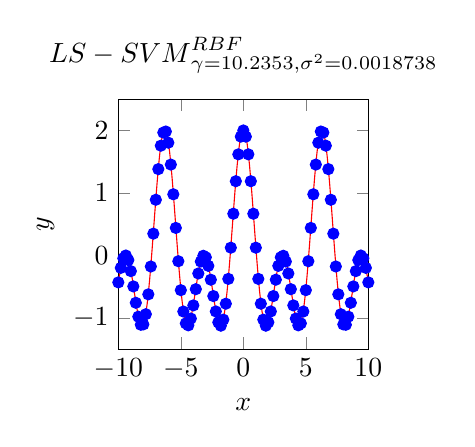
\begin{tikzpicture}

\begin{axis}[%
width=1.25in,
height=1.25in,
scale only axis,
xmin=-10,
xmax=10,
ymin=-1.5,
ymax=2.5,
xlabel={$x$},
ylabel={$y$},
title={$\text{LS-SVM}_{\gamma\text{=10.2353,}\sigma{}^\text{2}\text{=0.0018738}}^{\text{RBF}}$}
]
\addplot [color=red,solid,forget plot]
  table[row sep=crcr]{%
-10	-0.382794158226064\\
-9.9	-0.31542840514059\\
-9.8	-0.209290617485432\\
-9.7	-0.104436022691509\\
-9.6	-0.0297589748378465\\
-9.5	0.00663716354359287\\
-9.4	0.0096355322687327\\
-9.3	-0.0149546002203966\\
-9.2	-0.0652342563197698\\
-9.1	-0.140837854254202\\
-9	-0.239461306292531\\
-8.9	-0.356018924144576\\
-8.8	-0.483820578485325\\
-8.7	-0.615793609533385\\
-8.6	-0.744898148294766\\
-8.5	-0.864093769334848\\
-8.4	-0.966407044022721\\
-8.3	-1.0452424072567\\
-8.2	-1.09477353299107\\
-8.1	-1.11025545510458\\
-8	-1.08822758507005\\
-7.9	-1.02665004337803\\
-7.8	-0.925003225144367\\
-7.7	-0.784344808013278\\
-7.6	-0.607305745057128\\
-7.5	-0.398016940131312\\
-7.4	-0.161971365179353\\
-7.3	0.0941685724729631\\
-7.2	0.362809341644915\\
-7.1	0.635702051778293\\
-7	0.904246204539089\\
-6.9	1.15980985134934\\
-6.8	1.39405324457815\\
-6.7	1.5992429595825\\
-6.6	1.76854412486773\\
-6.5	1.89627939379904\\
-6.4	1.97814454725007\\
-6.3	2.0113722309383\\
-6.2	1.99483734071776\\
-6.1	1.92909988617777\\
-6	1.81638364981747\\
-5.9	1.66049149332931\\
-5.8	1.46666065143462\\
-5.7	1.24136371057889\\
-5.6	0.992063106422413\\
-5.5	0.726928801642829\\
-5.4	0.454530248655517\\
-5.3	0.183514741825927\\
-5.2	-0.077715217428287\\
-5.1	-0.321312901377876\\
-5	-0.540274524746607\\
-4.9	-0.728691409255073\\
-4.8	-0.881957361232854\\
-4.7	-0.996923276280318\\
-4.6	-1.07199309754855\\
-4.5	-1.10715759762228\\
-4.4	-1.10396493557649\\
-4.3	-1.06542946074504\\
-4.2	-0.99588269352447\\
-4.1	-0.900772712260995\\
-4	-0.786420223182846\\
-3.9	-0.659741305127812\\
-3.8	-0.527948134891837\\
-3.7	-0.39823985962466\\
-3.6	-0.277496156059067\\
-3.5	-0.171985887578727\\
-3.4	-0.0871026445990545\\
-3.3	-0.0271378567542622\\
-3.2	0.00489935934604218\\
-3.1	0.00740834402301428\\
-3	-0.0197360605220089\\
-2.9	-0.0751782694699391\\
-2.8	-0.156138730201734\\
-2.7	-0.258530422037382\\
-2.6	-0.377130379499935\\
-2.5	-0.505799315297361\\
-2.4	-0.637740473378351\\
-2.3	-0.765787251583269\\
-2.2	-0.8827079608175\\
-2.1	-0.981515380634931\\
-2	-1.05576855790684\\
-1.9	-1.09985458457369\\
-1.8	-1.1092388711787\\
-1.7	-1.08067367367067\\
-1.6	-1.01235628301824\\
-1.5	-0.904030284131657\\
-1.4	-0.757025553665023\\
-1.3	-0.574235104495459\\
-1.2	-0.360029401752693\\
-1.1	-0.12011126997515\\
-1	0.138683115310734\\
-0.9	0.40862950105121\\
-0.799999999999999	0.681397589224331\\
-0.699999999999999	0.948358843672728\\
-0.6	1.20090804265209\\
-0.5	1.43078598202661\\
-0.399999999999999	1.63039066740169\\
-0.299999999999999	1.79306476951503\\
-0.199999999999999	1.91334803900266\\
-0.0999999999999996	1.98718474728669\\
0	2.01207798600701\\
0.0999999999999996	1.98718474728669\\
0.199999999999999	1.91334803900266\\
0.299999999999999	1.79306476951503\\
0.399999999999999	1.63039066740169\\
0.5	1.43078598202661\\
0.6	1.20090804265209\\
0.699999999999999	0.948358843672728\\
0.799999999999999	0.681397589224331\\
0.9	0.40862950105121\\
1	0.138683115310734\\
1.1	-0.12011126997515\\
1.2	-0.360029401752693\\
1.3	-0.574235104495459\\
1.4	-0.757025553665023\\
1.5	-0.904030284131658\\
1.6	-1.01235628301824\\
1.7	-1.08067367367067\\
1.8	-1.1092388711787\\
1.9	-1.09985458457369\\
2	-1.05576855790684\\
2.1	-0.981515380634931\\
2.2	-0.8827079608175\\
2.3	-0.765787251583269\\
2.4	-0.637740473378351\\
2.5	-0.505799315297361\\
2.6	-0.377130379499935\\
2.7	-0.258530422037382\\
2.8	-0.156138730201734\\
2.9	-0.0751782694699391\\
3	-0.0197360605220089\\
3.1	0.00740834402301428\\
3.2	0.00489935934604217\\
3.3	-0.0271378567542622\\
3.4	-0.0871026445990545\\
3.5	-0.171985887578727\\
3.6	-0.277496156059067\\
3.7	-0.39823985962466\\
3.8	-0.527948134891836\\
3.9	-0.659741305127812\\
4	-0.786420223182846\\
4.1	-0.900772712260995\\
4.2	-0.99588269352447\\
4.3	-1.06542946074504\\
4.4	-1.10396493557649\\
4.5	-1.10715759762228\\
4.6	-1.07199309754855\\
4.7	-0.996923276280318\\
4.8	-0.881957361232854\\
4.9	-0.728691409255073\\
5	-0.540274524746607\\
5.1	-0.321312901377876\\
5.2	-0.0777152174282869\\
5.3	0.183514741825927\\
5.4	0.454530248655517\\
5.5	0.726928801642829\\
5.6	0.992063106422413\\
5.7	1.24136371057889\\
5.8	1.46666065143462\\
5.9	1.66049149332931\\
6	1.81638364981747\\
6.1	1.92909988617777\\
6.2	1.99483734071777\\
6.3	2.0113722309383\\
6.4	1.97814454725007\\
6.5	1.89627939379904\\
6.6	1.76854412486773\\
6.7	1.59924295958251\\
6.8	1.39405324457815\\
6.9	1.15980985134934\\
7	0.904246204539089\\
7.1	0.635702051778293\\
7.2	0.362809341644915\\
7.3	0.094168572472963\\
7.4	-0.161971365179353\\
7.5	-0.398016940131312\\
7.6	-0.607305745057127\\
7.7	-0.784344808013277\\
7.8	-0.925003225144366\\
7.9	-1.02665004337803\\
8	-1.08822758507005\\
8.1	-1.11025545510458\\
8.2	-1.09477353299107\\
8.3	-1.0452424072567\\
8.4	-0.966407044022721\\
8.5	-0.864093769334848\\
8.6	-0.744898148294766\\
8.7	-0.615793609533385\\
8.8	-0.483820578485325\\
8.9	-0.356018924144576\\
9	-0.239461306292531\\
9.1	-0.140837854254202\\
9.2	-0.0652342563197698\\
9.3	-0.0149546002203966\\
9.4	0.00963553226873268\\
9.5	0.00663716354359287\\
9.6	-0.0297589748378465\\
9.7	-0.104436022691509\\
9.8	-0.209290617485432\\
9.9	-0.31542840514059\\
10	-0.382794158226064\\
};
\addplot [color=blue,only marks,mark=*,mark options={solid},forget plot]
  table[row sep=crcr]{%
-10	-0.43098946726306\\
-9.8	-0.199040176459257\\
-9.6	-0.0454675090972562\\
-9.4	-0.000920685447996283\\
-9.2	-0.0742034490193951\\
-9	-0.250813553640597\\
-8.8	-0.495349259142413\\
-8.6	-0.757398242051853\\
-8.4	-0.979967241528048\\
-8.2	-1.10910282152591\\
-8	-1.103159514132\\
-7.8	-0.940222204621165\\
-7.6	-0.622477140428825\\
-7.4	-0.17680515538033\\
-7.2	0.348533958318501\\
-7	0.890639472551138\\
-6.8	1.38110148280297\\
-6.6	1.75611654959898\\
-6.4	1.96601748445563\\
-6.2	1.98273439930208\\
-6	1.80402424538286\\
-5.8	1.45380914670929\\
-5.6	0.978570742329\\
-5.4	0.440362969487297\\
-5.2	-0.0924675861268539\\
-5	-0.555409343613226\\
-4.8	-0.897188872354681\\
-4.6	-1.08699614833922\\
-4.4	-1.11842588404008\\
-4.2	-1.00954947545738\\
-4	-0.799143654672225\\
-3.8	-0.539707869332161\\
-3.6	-0.288407101801892\\
-3.4	-0.0974007022296354\\
-3.2	-0.00510985703656031\\
-3	-0.0298222099500793\\
-2.8	-0.166656462158408\\
-2.6	-0.388372082068571\\
-2.4	-0.6498947321018\\
-2.2	-0.895833987233766\\
-2	-1.06979045741075\\
-1.8	-1.12396051102723\\
-1.6	-1.02749429809604\\
-1.4	-0.772255197768418\\
-1.2	-0.37503596106457\\
-1	0.124155469320997\\
-0.799999999999999	0.66750718704588\\
-0.6	1.18769336938635\\
-0.399999999999999	1.61776770335005\\
-0.199999999999999	1.90112757184413\\
0	2\\
0.199999999999999	1.90112757184413\\
0.399999999999999	1.61776770335005\\
0.6	1.18769336938635\\
0.799999999999999	0.66750718704588\\
1	0.124155469320997\\
1.2	-0.37503596106457\\
1.4	-0.772255197768418\\
1.6	-1.02749429809604\\
1.8	-1.12396051102723\\
2	-1.06979045741075\\
2.2	-0.895833987233766\\
2.4	-0.6498947321018\\
2.6	-0.388372082068571\\
2.8	-0.166656462158408\\
3	-0.0298222099500793\\
3.2	-0.00510985703656031\\
3.4	-0.0974007022296354\\
3.6	-0.288407101801892\\
3.8	-0.539707869332161\\
4	-0.799143654672225\\
4.2	-1.00954947545738\\
4.4	-1.11842588404008\\
4.6	-1.08699614833922\\
4.8	-0.897188872354681\\
5	-0.555409343613226\\
5.2	-0.0924675861268539\\
5.4	0.440362969487297\\
5.6	0.978570742329\\
5.8	1.45380914670929\\
6	1.80402424538286\\
6.2	1.98273439930208\\
6.4	1.96601748445563\\
6.6	1.75611654959898\\
6.8	1.38110148280297\\
7	0.890639472551138\\
7.2	0.348533958318501\\
7.4	-0.17680515538033\\
7.6	-0.622477140428825\\
7.8	-0.940222204621165\\
8	-1.103159514132\\
8.2	-1.10910282152591\\
8.4	-0.979967241528048\\
8.6	-0.757398242051853\\
8.8	-0.495349259142413\\
9	-0.250813553640597\\
9.2	-0.0742034490193951\\
9.4	-0.000920685447996283\\
9.6	-0.0454675090972562\\
9.8	-0.199040176459257\\
10	-0.43098946726306\\
};
\end{axis}
\end{tikzpicture}%
\end{document}
% This file was created by matlab2tikz.
% Minimal pgfplots version: 1.3
%
%The latest updates can be retrieved from
%  http://www.mathworks.com/matlabcentral/fileexchange/22022-matlab2tikz
%where you can also make suggestions and rate matlab2tikz.
%
\documentclass[tikz]{standalone}
\usepackage{pgfplots}
\usepackage{grffile}
\pgfplotsset{compat=newest}
\usetikzlibrary{plotmarks}
\usepackage{amsmath}

\begin{document}
\definecolor{mycolor1}{rgb}{0.00000,0.44700,0.74100}%
\definecolor{mycolor2}{rgb}{0.85000,0.32500,0.09800}%
%
\begin{tikzpicture}

\begin{axis}[%
width=1.25in,
height=1.25in,
scale only axis,
xmin=-10,
xmax=10,
ymin=-1.5,
ymax=2.5,
xlabel={$x$},
ylabel={$y$},
legend style={legend cell align=left,align=left,draw=white!15!black}
]
\addplot [color=mycolor1,only marks,mark=*,mark options={solid}]
  table[row sep=crcr]{%
-9.9	-0.307869340810925\\
-9.7	-0.110072555965846\\
-9.5	-0.00846753800970923\\
-9.3	-0.0232031325135535\\
-9.1	-0.151369131839189\\
-8.9	-0.367479006452697\\
-8.7	-0.627703045668925\\
-8.5	-0.877175240736421\\
-8.3	-1.05920488021701\\
-8.1	-1.12491664409803\\
-7.9	-1.04176973451283\\
-7.7	-0.799579054849314\\
-7.5	-0.413052595023795\\
-7.3	0.0795926259688397\\
-7.1	0.621754943518725\\
-6.9	1.1465399780744\\
-6.7	1.58657623178879\\
-6.5	1.88403440717822\\
-6.3	1.99929322188442\\
-6.1	1.91690208251722\\
-5.9	1.64791090973487\\
-5.7	1.22820365118705\\
-5.5	0.713095472279311\\
-5.3	0.169036145407331\\
-5.1	-0.33628790931422\\
-4.9	-0.743913902682179\\
-4.7	-1.0120817054981\\
-4.5	-1.12192606131546\\
-4.3	-1.07951921939999\\
-4.1	-0.913978807517104\\
-3.9	-0.67197688363749\\
-3.7	-0.409552704136017\\
-3.5	-0.182554432947492\\
-3.3	-0.0372471779503353\\
-3.1	-0.00259305325006209\\
-2.9	-0.085438648208272\\
-2.7	-0.269379266074428\\
-2.5	-0.517481430083707\\
-2.3	-0.778428548214879\\
-2.1	-0.995106925940557\\
-1.9	-1.11425727877792\\
-1.7	-1.09564268687499\\
-1.5	-0.919255294932742\\
-1.3	-0.589389924744358\\
-1.1	-0.134904995829767\\
-0.9	0.394407873577576\\
-0.699999999999999	0.934809330184731\\
-0.5	1.41788486775851\\
-0.299999999999999	1.78067210403529\\
-0.0999999999999996	1.97507074311927\\
0.0999999999999996	1.97507074311927\\
0.299999999999999	1.78067210403529\\
0.5	1.41788486775851\\
0.699999999999999	0.934809330184731\\
0.9	0.394407873577576\\
1.1	-0.134904995829767\\
1.3	-0.589389924744358\\
1.5	-0.919255294932742\\
1.7	-1.09564268687499\\
1.9	-1.11425727877792\\
2.1	-0.995106925940557\\
2.3	-0.778428548214879\\
2.5	-0.517481430083707\\
2.7	-0.269379266074428\\
2.9	-0.085438648208272\\
3.1	-0.00259305325006209\\
3.3	-0.0372471779503353\\
3.5	-0.182554432947492\\
3.7	-0.409552704136017\\
3.9	-0.67197688363749\\
4.1	-0.913978807517104\\
4.3	-1.07951921939999\\
4.5	-1.12192606131546\\
4.7	-1.0120817054981\\
4.9	-0.743913902682179\\
5.1	-0.33628790931422\\
5.3	0.169036145407331\\
5.5	0.713095472279311\\
5.7	1.22820365118705\\
5.9	1.64791090973487\\
6.1	1.91690208251722\\
6.3	1.99929322188442\\
6.5	1.88403440717822\\
6.7	1.58657623178879\\
6.9	1.1465399780744\\
7.1	0.621754943518725\\
7.3	0.0795926259688397\\
7.5	-0.413052595023795\\
7.7	-0.799579054849314\\
7.9	-1.04176973451283\\
8.1	-1.12491664409803\\
8.3	-1.05920488021701\\
8.5	-0.877175240736421\\
8.7	-0.627703045668925\\
8.9	-0.367479006452697\\
9.1	-0.151369131839189\\
9.3	-0.0232031325135535\\
9.5	-0.00846753800970923\\
9.7	-0.110072555965846\\
9.9	-0.307869340810925\\
};

\addplot [color=mycolor2,only marks,mark=+,mark options={solid}]
  table[row sep=crcr]{%
-9.9	-0.31542840514059\\
-9.7	-0.104436022691509\\
-9.5	0.00663716354359287\\
-9.3	-0.0149546002203966\\
-9.1	-0.140837854254202\\
-8.9	-0.356018924144576\\
-8.7	-0.615793609533385\\
-8.5	-0.864093769334848\\
-8.3	-1.0452424072567\\
-8.1	-1.11025545510458\\
-7.9	-1.02665004337803\\
-7.7	-0.784344808013278\\
-7.5	-0.398016940131312\\
-7.3	0.0941685724729631\\
-7.1	0.635702051778293\\
-6.9	1.15980985134934\\
-6.7	1.5992429595825\\
-6.5	1.89627939379904\\
-6.3	2.0113722309383\\
-6.1	1.92909988617777\\
-5.9	1.66049149332931\\
-5.7	1.24136371057889\\
-5.5	0.726928801642829\\
-5.3	0.183514741825927\\
-5.1	-0.321312901377876\\
-4.9	-0.728691409255073\\
-4.7	-0.996923276280318\\
-4.5	-1.10715759762228\\
-4.3	-1.06542946074504\\
-4.1	-0.900772712260995\\
-3.9	-0.659741305127812\\
-3.7	-0.39823985962466\\
-3.5	-0.171985887578727\\
-3.3	-0.0271378567542622\\
-3.1	0.00740834402301428\\
-2.9	-0.0751782694699391\\
-2.7	-0.258530422037382\\
-2.5	-0.505799315297361\\
-2.3	-0.765787251583269\\
-2.1	-0.981515380634931\\
-1.9	-1.09985458457369\\
-1.7	-1.08067367367067\\
-1.5	-0.904030284131657\\
-1.3	-0.574235104495459\\
-1.1	-0.12011126997515\\
-0.9	0.40862950105121\\
-0.699999999999999	0.948358843672728\\
-0.5	1.43078598202661\\
-0.299999999999999	1.79306476951503\\
-0.0999999999999996	1.98718474728669\\
0.0999999999999996	1.98718474728669\\
0.299999999999999	1.79306476951503\\
0.5	1.43078598202661\\
0.699999999999999	0.948358843672728\\
0.9	0.40862950105121\\
1.1	-0.12011126997515\\
1.3	-0.574235104495459\\
1.5	-0.904030284131658\\
1.7	-1.08067367367067\\
1.9	-1.09985458457369\\
2.1	-0.981515380634931\\
2.3	-0.765787251583269\\
2.5	-0.505799315297361\\
2.7	-0.258530422037382\\
2.9	-0.0751782694699391\\
3.1	0.00740834402301428\\
3.3	-0.0271378567542622\\
3.5	-0.171985887578727\\
3.7	-0.39823985962466\\
3.9	-0.659741305127812\\
4.1	-0.900772712260995\\
4.3	-1.06542946074504\\
4.5	-1.10715759762228\\
4.7	-0.996923276280318\\
4.9	-0.728691409255073\\
5.1	-0.321312901377876\\
5.3	0.183514741825927\\
5.5	0.726928801642829\\
5.7	1.24136371057889\\
5.9	1.66049149332931\\
6.1	1.92909988617777\\
6.3	2.0113722309383\\
6.5	1.89627939379904\\
6.7	1.59924295958251\\
6.9	1.15980985134934\\
7.1	0.635702051778293\\
7.3	0.094168572472963\\
7.5	-0.398016940131312\\
7.7	-0.784344808013277\\
7.9	-1.02665004337803\\
8.1	-1.11025545510458\\
8.3	-1.0452424072567\\
8.5	-0.864093769334848\\
8.7	-0.615793609533385\\
8.9	-0.356018924144576\\
9.1	-0.140837854254202\\
9.3	-0.0149546002203966\\
9.5	0.00663716354359287\\
9.7	-0.104436022691509\\
9.9	-0.31542840514059\\
};
\end{axis}
\end{tikzpicture}%
\end{document}
% This file was created by matlab2tikz.
% Minimal pgfplots version: 1.3
%
%The latest updates can be retrieved from
%  http://www.mathworks.com/matlabcentral/fileexchange/22022-matlab2tikz
%where you can also make suggestions and rate matlab2tikz.
%
\documentclass[tikz]{standalone}
\usepackage{pgfplots}
\usepackage{grffile}
\pgfplotsset{compat=newest}
\usetikzlibrary{plotmarks}
\usepackage{amsmath}

\begin{document}
\begin{tikzpicture}

\begin{axis}[%
width=1.25in,
height=1.25in,
scale only axis,
xmin=-5,
xmax=0,
xlabel={$\sigma^2$},
xmajorgrids,
ymin=0,
ymax=10,
ylabel={$\gamma$},
ymajorgrids,
zmin=0,
zmax=10,
zmajorgrids,
view={90}{90},
axis x line*=bottom,
axis y line*=left,
axis z line*=left
]

\addplot3[%
surf,
shader=flat,
colormap={mymap}{[1pt] rgb(0pt)=(0.2081,0.1663,0.5292); rgb(1pt)=(0.211624,0.189781,0.577676); rgb(2pt)=(0.212252,0.213771,0.626971); rgb(3pt)=(0.2081,0.2386,0.677086); rgb(4pt)=(0.195905,0.264457,0.7279); rgb(5pt)=(0.170729,0.291938,0.779248); rgb(6pt)=(0.125271,0.324243,0.830271); rgb(7pt)=(0.0591333,0.359833,0.868333); rgb(8pt)=(0.0116952,0.38751,0.881957); rgb(9pt)=(0.00595714,0.408614,0.882843); rgb(10pt)=(0.0165143,0.4266,0.878633); rgb(11pt)=(0.0328524,0.443043,0.871957); rgb(12pt)=(0.0498143,0.458571,0.864057); rgb(13pt)=(0.0629333,0.47369,0.855438); rgb(14pt)=(0.0722667,0.488667,0.8467); rgb(15pt)=(0.0779429,0.503986,0.838371); rgb(16pt)=(0.0793476,0.520024,0.831181); rgb(17pt)=(0.0749429,0.537543,0.826271); rgb(18pt)=(0.0640571,0.556986,0.823957); rgb(19pt)=(0.0487714,0.577224,0.822829); rgb(20pt)=(0.0343429,0.596581,0.819852); rgb(21pt)=(0.0265,0.6137,0.8135); rgb(22pt)=(0.0238905,0.628662,0.803762); rgb(23pt)=(0.0230905,0.641786,0.791267); rgb(24pt)=(0.0227714,0.653486,0.776757); rgb(25pt)=(0.0266619,0.664195,0.760719); rgb(26pt)=(0.0383714,0.674271,0.743552); rgb(27pt)=(0.0589714,0.683757,0.725386); rgb(28pt)=(0.0843,0.692833,0.706167); rgb(29pt)=(0.113295,0.7015,0.685857); rgb(30pt)=(0.145271,0.709757,0.664629); rgb(31pt)=(0.180133,0.717657,0.642433); rgb(32pt)=(0.217829,0.725043,0.619262); rgb(33pt)=(0.258643,0.731714,0.595429); rgb(34pt)=(0.302171,0.737605,0.571186); rgb(35pt)=(0.348167,0.742433,0.547267); rgb(36pt)=(0.395257,0.7459,0.524443); rgb(37pt)=(0.44201,0.748081,0.503314); rgb(38pt)=(0.487124,0.749062,0.483976); rgb(39pt)=(0.530029,0.749114,0.466114); rgb(40pt)=(0.570857,0.748519,0.44939); rgb(41pt)=(0.609852,0.747314,0.433686); rgb(42pt)=(0.6473,0.7456,0.4188); rgb(43pt)=(0.683419,0.743476,0.404433); rgb(44pt)=(0.71841,0.741133,0.390476); rgb(45pt)=(0.752486,0.7384,0.376814); rgb(46pt)=(0.785843,0.735567,0.363271); rgb(47pt)=(0.818505,0.732733,0.34979); rgb(48pt)=(0.850657,0.7299,0.336029); rgb(49pt)=(0.882433,0.727433,0.3217); rgb(50pt)=(0.913933,0.725786,0.306276); rgb(51pt)=(0.944957,0.726114,0.288643); rgb(52pt)=(0.973895,0.731395,0.266648); rgb(53pt)=(0.993771,0.745457,0.240348); rgb(54pt)=(0.999043,0.765314,0.216414); rgb(55pt)=(0.995533,0.786057,0.196652); rgb(56pt)=(0.988,0.8066,0.179367); rgb(57pt)=(0.978857,0.827143,0.163314); rgb(58pt)=(0.9697,0.848138,0.147452); rgb(59pt)=(0.962586,0.870514,0.1309); rgb(60pt)=(0.958871,0.8949,0.113243); rgb(61pt)=(0.959824,0.921833,0.0948381); rgb(62pt)=(0.9661,0.951443,0.0755333); rgb(63pt)=(0.9763,0.9831,0.0538)},
mesh/rows=100]
table[row sep=crcr,header=false] {%
%
-5	0	9.71913607767262\\
-5	0.101010101010101	9.71911750564431\\
-5	0.202020202020202	9.71904418634401\\
-5	0.303030303030303	9.71879791694858\\
-5	0.404040404040404	9.7180818123259\\
-5	0.505050505050505	9.7162509394907\\
-5	0.606060606060606	9.71207761892269\\
-5	0.707070707070707	9.70349079909844\\
-5	0.808080808080808	9.68736500946506\\
-5	0.909090909090909	9.65944957142862\\
-5	1.01010101010101	9.61450894316157\\
-5	1.11111111111111	9.54669336749995\\
-5	1.21212121212121	9.45009473822307\\
-5	1.31313131313131	9.31939083107305\\
-5	1.41414141414141	9.15046009897336\\
-5	1.51515151515152	8.9408640471654\\
-5	1.61616161616162	8.69013698312136\\
-5	1.71717171717172	8.39987770380502\\
-5	1.81818181818182	8.07368504121225\\
-5	1.91919191919192	7.71700099733868\\
-5	2.02020202020202	7.33691091130872\\
-5	2.12121212121212	6.94190387004145\\
-5	2.22222222222222	6.54154058932441\\
-5	2.32323232323232	6.14594517349589\\
-5	2.42424242424242	5.76506363860231\\
-5	2.52525252525253	5.40772353151497\\
-5	2.62626262626263	5.08065291162341\\
-5	2.72727272727273	4.7877076396922\\
-5	2.82828282828283	4.52954980553097\\
-5	2.92929292929293	4.30390056437419\\
-5	3.03030303030303	4.10630624653053\\
-5	3.13131313131313	3.93119429348256\\
-5	3.23232323232323	3.77292749194009\\
-5	3.33333333333333	3.62660953115934\\
-5	3.43434343434343	3.4885161490052\\
-5	3.53535353535354	3.35616259586319\\
-5	3.63636363636364	3.22811616900113\\
-5	3.73737373737374	3.10369662354881\\
-5	3.83838383838384	2.9826835158267\\
-5	3.93939393939394	2.86509571613909\\
-5	4.04040404040404	2.75105602808426\\
-5	4.14141414141414	2.64072259193151\\
-5	4.24242424242424	2.53426060975256\\
-5	4.34343434343434	2.43183363775986\\
-5	4.44444444444444	2.33360273365613\\
-5	4.54545454545455	2.2397284093262\\
-5	4.64646464646465	2.15037372580039\\
-5	4.74747474747475	2.06570816729336\\
-5	4.84848484848485	1.98591233528186\\
-5	4.94949494949495	1.91118362604005\\
-5	5.05050505050505	1.84174311369983\\
-5	5.15151515151515	1.77784391698977\\
-5	5.25252525252525	1.71978139767602\\
-5	5.35353535353535	1.66790562786053\\
-5	5.45454545454545	1.62263667549202\\
-5	5.55555555555556	1.58448339741348\\
-5	5.65656565656566	1.55406660283488\\
-5	5.75757575757576	1.53214766307313\\
-5	5.85858585858586	1.51966389791168\\
-5	5.95959595959596	1.5177723543103\\
-5	6.06060606060606	1.52790386459116\\
-5	6.16161616161616	1.55182940492681\\
-5	6.26262626262626	1.59174048221436\\
-5	6.36363636363636	1.65034395125362\\
-5	6.46464646464646	1.7309681302233\\
-5	6.56565656565657	1.83766924237365\\
-5	6.66666666666667	1.97531165568672\\
-5	6.76767676767677	2.14956735369417\\
-5	6.86868686868687	2.36673489197302\\
-5	6.96969696969697	2.63321700746984\\
-5	7.07070707070707	2.95444100975846\\
-5	7.17171717171717	3.33302583056566\\
-5	7.27272727272727	3.76622725461807\\
-5	7.37373737373737	4.2432604247124\\
-5	7.47474747474747	4.74388776505789\\
-5	7.57575757575758	5.24001570264461\\
-5	7.67676767676768	5.70110740936049\\
-5	7.77777777777778	6.10205980317231\\
-5	7.87878787878788	6.43023673373301\\
-5	7.97979797979798	6.68822881517376\\
-5	8.08080808080808	6.89114742998409\\
-5	8.18181818181818	7.06055550358695\\
-5	8.28282828282828	7.21869414860415\\
-5	8.38383838383838	7.3849216894615\\
-5	8.48484848484848	7.57344650989021\\
-5	8.58585858585859	7.79104669628234\\
-5	8.68686868686869	8.03552862169154\\
-5	8.78787878787879	8.29668877762188\\
-5	8.88888888888889	8.55976448412853\\
-5	8.98989898989899	8.80934281835338\\
-5	9.09090909090909	9.03210457300771\\
-5	9.19191919191919	9.21848909899515\\
-5	9.29292929292929	9.36388121975823\\
-5	9.39393939393939	9.46911977743927\\
-5	9.49494949494949	9.53971958832904\\
-5	9.5959595959596	9.58389607753167\\
-5	9.6969696969697	9.61029331846618\\
-5	9.7979797979798	9.62630675103364\\
-5	9.8989898989899	9.63729997148607\\
-5	10	9.64653377687649\\
-4.94949494949495	0	9.71913553273757\\
-4.94949494949495	0.101010101010101	9.71911481061148\\
-4.94949494949495	0.202020202020202	9.71903300308032\\
-4.94949494949495	0.303030303030303	9.71875822289079\\
-4.94949494949495	0.404040404040404	9.71795921429561\\
-4.94949494949495	0.505050505050505	9.71591637993825\\
-4.94949494949495	0.606060606060606	9.71125991095614\\
-4.94949494949495	0.707070707070707	9.70167898881465\\
-4.94949494949495	0.808080808080808	9.68368630554105\\
-4.94949494949495	0.909090909090909	9.65253908025972\\
-4.94949494949495	1.01010101010101	9.60239565369832\\
-4.94949494949495	1.11111111111111	9.52672905067613\\
-4.94949494949495	1.21212121212121	9.41894721417478\\
-4.94949494949495	1.31313131313131	9.27311188457066\\
-4.94949494949495	1.41414141414141	9.08462484731077\\
-4.94949494949495	1.51515151515152	8.85076714226605\\
-4.94949494949495	1.61616161616162	8.57102524209201\\
-4.94949494949495	1.71717171717172	8.24720023534336\\
-4.94949494949495	1.81818181818182	7.88334941093546\\
-4.94949494949495	1.91919191919192	7.48563294404459\\
-4.94949494949495	2.02020202020202	7.06211886753633\\
-4.94949494949495	2.12121212121212	6.62254210478146\\
-4.94949494949495	2.22222222222222	6.17794517386064\\
-4.94949494949495	2.32323232323232	5.74009233085246\\
-4.94949494949495	2.42424242424242	5.32058513170202\\
-4.94949494949495	2.52525252525253	4.92972455142994\\
-4.94949494949495	2.62626262626263	4.57532077638409\\
-4.94949494949495	2.72727272727273	4.26176254315805\\
-4.94949494949495	2.82828282828283	3.98964400231237\\
-4.94949494949495	2.92929292929293	3.75609148106349\\
-4.94949494949495	3.03030303030303	3.55570186650517\\
-4.94949494949495	3.13131313131313	3.38181012420421\\
-4.94949494949495	3.23232323232323	3.22773193977893\\
-4.94949494949495	3.33333333333333	3.08769329720255\\
-4.94949494949495	3.43434343434343	2.95731076749716\\
-4.94949494949495	3.53535353535354	2.83364778363676\\
-4.94949494949495	3.63636363636364	2.71498197901506\\
-4.94949494949495	3.73737373737374	2.60045171368628\\
-4.94949494949495	3.83838383838384	2.48971753942583\\
-4.94949494949495	3.93939393939394	2.38271036093417\\
-4.94949494949495	4.04040404040404	2.27947830970724\\
-4.94949494949495	4.14141414141414	2.18010980645011\\
-4.94949494949495	4.24242424242424	2.08470210181173\\
-4.94949494949495	4.34343434343434	1.99335166557609\\
-4.94949494949495	4.44444444444444	1.90615322624955\\
-4.94949494949495	4.54545454545455	1.82320179315828\\
-4.94949494949495	4.64646464646465	1.74459577940731\\
-4.94949494949495	4.74747474747475	1.6704407914925\\
-4.94949494949495	4.84848484848485	1.60085410245284\\
-4.94949494949495	4.94949494949495	1.53596995927731\\
-4.94949494949495	5.05050505050505	1.47594593215319\\
-4.94949494949495	5.15151515151515	1.42097056294369\\
-4.94949494949495	5.25252525252525	1.37127263308959\\
-4.94949494949495	5.35353535353535	1.32713245401412\\
-4.94949494949495	5.45454545454545	1.28889569158744\\
-4.94949494949495	5.55555555555556	1.256990378643\\
-4.94949494949495	5.65656565656566	1.23194795897116\\
-4.94949494949495	5.75757575757576	1.21442946109189\\
-4.94949494949495	5.85858585858586	1.20525824322488\\
-4.94949494949495	5.95959595959596	1.20546120328296\\
-4.94949494949495	6.06060606060606	1.21632091115499\\
-4.94949494949495	6.16161616161616	1.23944173762753\\
-4.94949494949495	6.26262626262626	1.2768335295036\\
-4.94949494949495	6.36363636363636	1.33101623630578\\
-4.94949494949495	6.46464646464646	1.40514712296662\\
-4.94949494949495	6.56565656565657	1.50316686038676\\
-4.94949494949495	6.66666666666667	1.62994837788941\\
-4.94949494949495	6.76767676767677	1.79140714109273\\
-4.94949494949495	6.86868686868687	1.99448544042693\\
-4.94949494949495	6.96969696969697	2.24684919009047\\
-4.94949494949495	7.07070707070707	2.5560401053974\\
-4.94949494949495	7.17171717171717	2.9277609708921\\
-4.94949494949495	7.27272727272727	3.36308373726255\\
-4.94949494949495	7.37373737373737	3.85490051519954\\
-4.94949494949495	7.47474747474747	4.38498686651481\\
-4.94949494949495	7.57575757575758	4.9240219345931\\
-4.94949494949495	7.67676767676768	5.43644206200377\\
-4.94949494949495	7.77777777777778	5.88947467138068\\
-4.94949494949495	7.87878787878788	6.26269807226185\\
-4.94949494949495	7.97979797979798	6.55343083232698\\
-4.94949494949495	8.08080808080808	6.77527100568702\\
-4.94949494949495	8.18181818181818	6.95129218606767\\
-4.94949494949495	8.28282828282828	7.10659801011641\\
-4.94949494949495	8.38383838383838	7.26382796134848\\
-4.94949494949495	8.48484848484848	7.44101601201917\\
-4.94949494949495	8.58585858585859	7.64921727998253\\
-4.94949494949495	8.68686868686869	7.8897921063615\\
-4.94949494949495	8.78787878787879	8.15406603098111\\
-4.94949494949495	8.88888888888889	8.4267717417977\\
-4.94949494949495	8.98989898989899	8.69106342277354\\
-4.94949494949495	9.09090909090909	8.93209679159825\\
-4.94949494949495	9.19191919191919	9.13864394726706\\
-4.94949494949495	9.29292929292929	9.30402843257122\\
-4.94949494949495	9.39393939393939	9.42694011194893\\
-4.94949494949495	9.49494949494949	9.51136793066104\\
-4.94949494949495	9.5959595959596	9.56506664489687\\
-4.94949494949495	9.6969696969697	9.59716189769916\\
-4.94949494949495	9.7979797979798	9.61603621477622\\
-4.94949494949495	9.8989898989899	9.62814215753041\\
-4.94949494949495	10	9.63768962713475\\
-4.8989898989899	0	9.71913500221671\\
-4.8989898989899	0.101010101010101	9.71911218686555\\
-4.8989898989899	0.202020202020202	9.71902211562753\\
-4.8989898989899	0.303030303030303	9.71871957878905\\
-4.8989898989899	0.404040404040404	9.71783985913242\\
-4.8989898989899	0.505050505050505	9.71559066989481\\
-4.8989898989899	0.606060606060606	9.71046383237399\\
-4.8989898989899	0.707070707070707	9.69991510319084\\
-4.8989898989899	0.808080808080808	9.68010490812664\\
-4.8989898989899	0.909090909090909	9.64581138113\\
-4.8989898989899	1.01010101010101	9.59060277908702\\
-4.8989898989899	1.11111111111111	9.50729282469058\\
-4.8989898989899	1.21212121212121	9.3886236087947\\
-4.8989898989899	1.31313131313131	9.22805715671073\\
-4.8989898989899	1.41414141414141	9.02053129449421\\
-4.8989898989899	1.51515151515152	8.76305438819433\\
-4.8989898989899	1.61616161616162	8.45506756508768\\
-4.8989898989899	1.71717171717172	8.09857230529498\\
-4.8989898989899	1.81818181818182	7.69808059350674\\
-4.8989898989899	1.91919191919192	7.26046934555759\\
-4.8989898989899	2.02020202020202	6.79479543332712\\
-4.8989898989899	2.12121212121212	6.31205803965328\\
-4.8989898989899	2.22222222222222	5.82481375791959\\
-4.8989898989899	2.32323232323232	5.34650886083604\\
-4.8989898989899	2.42424242424242	4.89044069410452\\
-4.8989898989899	2.52525252525253	4.46840638917059\\
-4.8989898989899	2.62626262626263	4.08928874303176\\
-4.8989898989899	2.72727272727273	3.7579611384186\\
-4.8989898989899	2.82828282828283	3.47486864563114\\
-4.8989898989899	2.92929292929293	3.23644481207714\\
-4.8989898989899	3.03030303030303	3.03624176143919\\
-4.8989898989899	3.13131313131313	2.86642442072518\\
-4.8989898989899	3.23232323232323	2.71920817127184\\
-4.8989898989899	3.33333333333333	2.58791100088749\\
-4.8989898989899	3.43434343434343	2.46747691781386\\
-4.8989898989899	3.53535353535354	2.35451428955391\\
-4.8989898989899	3.63636363636364	2.24701292192957\\
-4.8989898989899	3.73737373737374	2.14393394811496\\
-4.8989898989899	3.83838383838384	2.04482443194713\\
-4.8989898989899	3.93939393939394	1.94953408616323\\
-4.8989898989899	4.04040404040404	1.85804453525792\\
-4.8989898989899	4.14141414141414	1.77038408828967\\
-4.8989898989899	4.24242424242424	1.68659301191633\\
-4.8989898989899	4.34343434343434	1.6067128511373\\
-4.8989898989899	4.44444444444444	1.53078517092259\\
-4.8989898989899	4.54545454545455	1.45885346123121\\
-4.8989898989899	4.64646464646465	1.39096611119105\\
-4.8989898989899	4.74747474747475	1.32717994549041\\
-4.8989898989899	4.84848484848485	1.26756431453702\\
-4.8989898989899	4.94949494949495	1.21220587585179\\
-4.8989898989899	5.05050505050505	1.16121425720008\\
-4.8989898989899	5.15151515151515	1.11472883119383\\
-4.8989898989899	5.25252525252525	1.07292688126098\\
-4.8989898989899	5.35353535353535	1.03603350876238\\
-4.8989898989899	5.45454545454545	1.00433372756166\\
-4.8989898989899	5.55555555555556	0.97818732734845\\
-4.8989898989899	5.65656565656566	0.958047280662063\\
-4.8989898989899	5.75757575757576	0.944482751555488\\
-4.8989898989899	5.85858585858586	0.938208177613322\\
-4.8989898989899	5.95959595959596	0.940120488556353\\
-4.8989898989899	6.06060606060606	0.951347329904991\\
-4.8989898989899	6.16161616161616	0.973310168444557\\
-4.8989898989899	6.26262626262626	1.00780724510245\\
-4.8989898989899	6.36363636363636	1.05712216405507\\
-4.8989898989899	6.46464646464646	1.12416369530319\\
-4.8989898989899	6.56565656565657	1.21263955541044\\
-4.8989898989899	6.66666666666667	1.32725845433844\\
-4.8989898989899	6.76767676767677	1.4739348290182\\
-4.8989898989899	6.86868686868687	1.65992963860437\\
-4.8989898989899	6.96969696969697	1.89378462957333\\
-4.8989898989899	7.07070707070707	2.18478646838136\\
-4.8989898989899	7.17171717171717	2.54155366426639\\
-4.8989898989899	7.27272727272727	2.96929720323054\\
-4.8989898989899	7.37373737373737	3.46566992752722\\
-4.8989898989899	7.47474747474747	4.01626158343736\\
-4.8989898989899	7.57575757575758	4.59246036115006\\
-4.8989898989899	7.67676767676768	5.15486535117437\\
-4.8989898989899	7.77777777777778	5.66288394840956\\
-4.8989898989899	7.87878787878788	6.08688094758102\\
-4.8989898989899	7.97979797979798	6.41689292321638\\
-4.8989898989899	8.08080808080808	6.66339160385317\\
-4.8989898989899	8.18181818181818	6.85029675103639\\
-4.8989898989899	8.28282828282828	7.00551070875907\\
-4.8989898989899	8.38383838383838	7.15479506664699\\
-4.8989898989899	8.48484848484848	7.31970967502042\\
-4.8989898989899	8.58585858585859	7.51579032590981\\
-4.8989898989899	8.68686868686869	7.74894584369092\\
-4.8989898989899	8.78787878787879	8.01313181292901\\
-4.8989898989899	8.88888888888889	8.29294887064217\\
-4.8989898989899	8.98989898989899	8.56983951164602\\
-4.8989898989899	9.09090909090909	8.82725504406192\\
-4.8989898989899	9.19191919191919	9.05261854476681\\
-4.8989898989899	9.29292929292929	9.23766519023997\\
-4.8989898989899	9.39393939393939	9.37902546920063\\
-4.8989898989899	9.49494949494949	9.47876405123677\\
-4.8989898989899	9.5959595959596	9.54360682075034\\
-4.8989898989899	9.6969696969697	9.58274248372131\\
-4.8989898989899	9.7979797979798	9.60535889302269\\
-4.8989898989899	9.8989898989899	9.61898681650335\\
-4.8989898989899	10	9.62887059828238\\
-4.84848484848485	0	9.71913449903844\\
-4.84848484848485	0.101010101010101	9.71910969834527\\
-4.84848484848485	0.202020202020202	9.71901178930486\\
-4.84848484848485	0.303030303030303	9.71868292637169\\
-4.84848484848485	0.404040404040404	9.71772665543382\\
-4.84848484848485	0.505050505050505	9.71528174667421\\
-4.84848484848485	0.606060606060606	9.70970878302377\\
-4.84848484848485	0.707070707070707	9.69824212681299\\
-4.84848484848485	0.808080808080808	9.6767080932048\\
-4.84848484848485	0.909090909090909	9.63943042298607\\
-4.84848484848485	1.01010101010101	9.57941770259748\\
-4.84848484848485	1.11111111111111	9.48885833492314\\
-4.84848484848485	1.21212121212121	9.35986288292659\\
-4.84848484848485	1.31313131313131	9.18532458909983\\
-4.84848484848485	1.41414141414141	8.95974132374454\\
-4.84848484848485	1.51515151515152	8.67986317417171\\
-4.84848484848485	1.61616161616162	8.34508937927569\\
-4.84848484848485	1.71717171717172	7.95761463666502\\
-4.84848484848485	1.81818181818182	7.5223898320039\\
-4.84848484848485	1.91919191919192	7.04698770594614\\
-4.84848484848485	2.02020202020202	6.54143227632964\\
-4.84848484848485	2.12121212121212	6.0179684651004\\
-4.84848484848485	2.22222222222222	5.49065337682448\\
-4.84848484848485	2.32323232323232	4.97460458794607\\
-4.84848484848485	2.42424242424242	4.48480089795317\\
-4.84848484848485	2.52525252525253	4.03450876917756\\
-4.84848484848485	2.62626262626263	3.63363745947794\\
-4.84848484848485	2.72727272727273	3.28747946083526\\
-4.84848484848485	2.82828282828283	2.99625429562963\\
-4.84848484848485	2.92929292929293	2.75562926784923\\
-4.84848484848485	3.03030303030303	2.55805451184075\\
-4.84848484848485	3.13131313131313	2.39449106688403\\
-4.84848484848485	3.23232323232323	2.25604295631529\\
-4.84848484848485	3.33333333333333	2.13512580731946\\
-4.84848484848485	3.43434343434343	2.02602562012569\\
-4.84848484848485	3.53535353535354	1.92491290672922\\
-4.84848484848485	3.63636363636364	1.82950607451244\\
-4.84848484848485	3.73737373737374	1.7386037387537\\
-4.84848484848485	3.83838383838384	1.65165292433966\\
-4.84848484848485	3.93939393939394	1.56843516992358\\
-4.84848484848485	4.04040404040404	1.48887880409852\\
-4.84848484848485	4.14141414141414	1.41296570804594\\
-4.84848484848485	4.24242424242424	1.34069334282366\\
-4.84848484848485	4.34343434343434	1.27206290005158\\
-4.84848484848485	4.44444444444444	1.20707761472571\\
-4.84848484848485	4.54545454545455	1.14574443435818\\
-4.84848484848485	4.64646464646465	1.08807674471976\\
-4.84848484848485	4.74747474747475	1.03409756784158\\
-4.84848484848485	4.84848484848485	0.983843194345212\\
-4.84848484848485	4.94949494949495	0.937367371865609\\
-4.84848484848485	5.05050505050505	0.894746218879445\\
-4.84848484848485	5.15151515151515	0.856084057547101\\
-4.84848484848485	5.25252525252525	0.821520391258001\\
-4.84848484848485	5.35353535353535	0.791238303789002\\
-4.84848484848485	5.45454545454545	0.765474636314097\\
-4.84848484848485	5.55555555555556	0.744532422436358\\
-4.84848484848485	5.65656565656566	0.728796258947673\\
-4.84848484848485	5.75757575757576	0.718751604825176\\
-4.84848484848485	5.85858585858586	0.715009489680698\\
-4.84848484848485	5.95959595959596	0.718338835762744\\
-4.84848484848485	6.06060606060606	0.729709598333124\\
-4.84848484848485	6.16161616161616	0.750351204102741\\
-4.84848484848485	6.26262626262626	0.781832227338623\\
-4.84848484848485	6.36363636363636	0.826168661913397\\
-4.84848484848485	6.46464646464646	0.885969049529278\\
-4.84848484848485	6.56565656565657	0.964624089992851\\
-4.84848484848485	6.66666666666667	1.0665439237865\\
-4.84848484848485	6.76767676767677	1.19743312704297\\
-4.84848484848485	6.86868686868687	1.36456173815348\\
-4.84848484848485	6.96969696969697	1.57692302310794\\
-4.84848484848485	7.07070707070707	1.84504176017116\\
-4.84848484848485	7.17171717171717	2.18000005967786\\
-4.84848484848485	7.27272727272727	2.59105142976785\\
-4.84848484848485	7.37373737373737	3.08128980936087\\
-4.84848484848485	7.47474747474747	3.64181784788564\\
-4.84848484848485	7.57575757575758	4.24705144706713\\
-4.84848484848485	7.67676767676768	4.85564814955163\\
-4.84848484848485	7.77777777777778	5.41971451057828\\
-4.84848484848485	7.87878787878788	5.89933599160219\\
-4.84848484848485	7.97979797979798	6.27517804445775\\
-4.84848484848485	8.08080808080808	6.55254469882411\\
-4.84848484848485	8.18181818181818	6.7551647263361\\
-4.84848484848485	8.28282828282828	6.91367998148507\\
-4.84848484848485	8.38383838383838	7.05697591488317\\
-4.84848484848485	8.48484848484848	7.20968197007742\\
-4.84848484848485	8.58585858585859	7.39154577462511\\
-4.84848484848485	8.68686868686869	7.61380112060538\\
-4.84848484848485	8.78787878787879	7.87450783206655\\
-4.84848484848485	8.88888888888889	8.1590189610203\\
-4.84848484848485	8.98989898989899	8.44681225783448\\
-4.84848484848485	9.09090909090909	8.71901540834906\\
-4.84848484848485	9.19191919191919	8.96165284776\\
-4.84848484848485	9.29292929292929	9.16541950186427\\
-4.84848484848485	9.39393939393939	9.32535223691445\\
-4.84848484848485	9.49494949494949	9.44149171543349\\
-4.84848484848485	9.5959595959596	9.51901480145763\\
-4.84848484848485	9.6969696969697	9.56664909600433\\
-4.84848484848485	9.7979797979798	9.59408928428821\\
-4.84848484848485	9.8989898989899	9.60985568598822\\
-4.84848484848485	10	9.62025963288485\\
-4.7979797979798	0	9.71913403347363\\
-4.7979797979798	0.101010101010101	9.71910739584617\\
-4.7979797979798	0.202020202020202	9.71900223489267\\
-4.7979797979798	0.303030303030303	9.71864901378594\\
-4.7979797979798	0.404040404040404	9.71762191390768\\
-4.7979797979798	0.505050505050505	9.71499591600056\\
-4.7979797979798	0.606060606060606	9.70901017493048\\
-4.7979797979798	0.707070707070707	9.69669420837375\\
-4.7979797979798	0.808080808080808	9.67356519632826\\
-4.7979797979798	0.909090909090909	9.63352645341447\\
-4.7979797979798	1.01010101010101	9.56906873281059\\
-4.7979797979798	1.11111111111111	9.47180186346878\\
-4.7979797979798	1.21212121212121	9.33325209421822\\
-4.7979797979798	1.31313131313131	9.14578642277979\\
-4.7979797979798	1.41414141414141	8.90349573116528\\
-4.7979797979798	1.51515151515152	8.60289143256427\\
-4.7979797979798	1.61616161616162	8.24333498337934\\
-4.7979797979798	1.71717171717172	7.82720259767014\\
-4.7979797979798	1.81818181818182	7.35985789157264\\
-4.7979797979798	1.91919191919192	6.84953132788466\\
-4.7979797979798	2.02020202020202	6.30716714821243\\
-4.7979797979798	2.12121212121212	5.74620320582822\\
-4.7979797979798	2.22222222222222	5.18214037005077\\
-4.7979797979798	2.32323232323232	4.63170720045918\\
-4.7979797979798	2.42424242424242	4.11149900367167\\
-4.7979797979798	2.52525252525253	3.63618097580166\\
-4.7979797979798	2.62626262626263	3.2166140338776\\
-4.7979797979798	2.72727272727273	2.85843658855902\\
-4.7979797979798	2.82828282828283	2.56158062508321\\
-4.7979797979798	2.92929292929293	2.3209062376986\\
-4.7979797979798	3.03030303030303	2.12774717834956\\
-4.7979797979798	3.13131313131313	1.97187154832229\\
-4.7979797979798	3.23232323232323	1.84330120894803\\
-4.7979797979798	3.33333333333333	1.73358728214315\\
-4.7979797979798	3.43434343434343	1.6363958565534\\
-4.7979797979798	3.53535353535354	1.54749286166664\\
-4.7979797979798	3.63636363636364	1.46435225552649\\
-4.7979797979798	3.73737373737374	1.38563167146589\\
-4.7979797979798	3.83838383838384	1.31069604565878\\
-4.7979797979798	3.93939393939394	1.23927477313245\\
-4.7979797979798	4.04040404040404	1.17125806647763\\
-4.7979797979798	4.14141414141414	1.10659621336542\\
-4.7979797979798	4.24242424242424	1.04525851062802\\
-4.7979797979798	4.34343434343434	0.987220241179646\\
-4.7979797979798	4.44444444444444	0.932460515500621\\
-4.7979797979798	4.54545454545455	0.88096367145589\\
-4.7979797979798	4.64646464646465	0.83272173436532\\
-4.7979797979798	4.74747474747475	0.787737268210567\\
-4.7979797979798	4.84848484848485	0.746026543173411\\
-4.7979797979798	4.94949494949495	0.707623119978975\\
-4.7979797979798	5.05050505050505	0.672581991282205\\
-4.7979797979798	5.15151515151515	0.640984424196941\\
-4.7979797979798	5.25252525252525	0.612943656285612\\
-4.7979797979798	5.35353535353535	0.588611626446573\\
-4.7979797979798	5.45454545454545	0.568186986289586\\
-4.7979797979798	5.55555555555556	0.551924762373899\\
-4.7979797979798	5.65656565656566	0.5401482672845\\
-4.7979797979798	5.75757575757576	0.533264244233597\\
-4.7979797979798	5.85858585858586	0.531782834448138\\
-4.7979797979798	5.95959595959596	0.536344818631822\\
-4.7979797979798	6.06060606060606	0.547759700091813\\
-4.7979797979798	6.16161616161616	0.567059515321349\\
-4.7979797979798	6.26262626262626	0.595574703078735\\
-4.7979797979798	6.36363636363636	0.63503987690412\\
-4.7979797979798	6.46464646464646	0.687738848987571\\
-4.7979797979798	6.56565656565657	0.756699375891504\\
-4.7979797979798	6.66666666666667	0.845947479279894\\
-4.7979797979798	6.76767676767677	0.960825076579385\\
-4.7979797979798	6.86868686868687	1.10835431444561\\
-4.7979797979798	6.96969696969697	1.29757969630632\\
-4.7979797979798	7.07070707070707	1.53970405780203\\
-4.7979797979798	7.17171717171717	1.84761888355842\\
-4.7979797979798	7.27272727272727	2.23411692277635\\
-4.7979797979798	7.37373737373737	2.70786979340984\\
-4.7979797979798	7.47474747474747	3.26681198938247\\
-4.7979797979798	7.57575757575758	3.89086432696212\\
-4.7979797979798	7.67676767676768	4.53933292000475\\
-4.7979797979798	7.77777777777778	5.15834117801946\\
-4.7979797979798	7.87878787878788	5.69715891525203\\
-4.7979797979798	7.97979797979798	6.12509719922371\\
-4.7979797979798	8.08080808080808	6.43989654607838\\
-4.7979797979798	8.18181818181818	6.66354391033537\\
-4.7979797979798	8.28282828282828	6.82921271265987\\
-4.7979797979798	8.38383838383838	6.96917497206035\\
-4.7979797979798	8.48484848484848	7.1107592400707\\
-4.7979797979798	8.58585858585859	7.27718072431223\\
-4.7979797979798	8.68686868686869	7.48521454773423\\
-4.7979797979798	8.78787878787879	7.73862678699919\\
-4.7979797979798	8.88888888888889	8.02513187186201\\
-4.7979797979798	8.98989898989899	8.32242789535296\\
-4.7979797979798	9.09090909090909	8.6084002114824\\
-4.7979797979798	9.19191919191919	8.86702193432879\\
-4.7979797979798	9.29292929292929	9.08824261122645\\
-4.7979797979798	9.39393939393939	9.26623214254529\\
-4.7979797979798	9.49494949494949	9.39932244799523\\
-4.7979797979798	9.5959595959596	9.49082219362479\\
-4.7979797979798	9.6969696969697	9.54843198218348\\
-4.7979797979798	9.7979797979798	9.58193458452621\\
-4.7979797979798	9.8989898989899	9.60066008205484\\
-4.7979797979798	10	9.61196164602542\\
-4.74747474747475	0	9.71913361248287\\
-4.74747474747475	0.101010101010101	9.71910531379269\\
-4.74747474747475	0.202020202020202	9.71899359523794\\
-4.74747474747475	0.303030303030303	9.71861834805516\\
-4.74747474747475	0.404040404040404	9.71752720053317\\
-4.74747474747475	0.505050505050505	9.71473745129677\\
-4.74747474747475	0.606060606060606	9.70837845290487\\
-4.74747474747475	0.707070707070707	9.69529449061844\\
-4.74747474747475	0.808080808080808	9.67072320654295\\
-4.74747474747475	0.909090909090909	9.62818774179355\\
-4.74747474747475	1.01010101010101	9.55971059532689\\
-4.74747474747475	1.11111111111111	9.45637841771093\\
-4.74747474747475	1.21212121212121	9.30918909196405\\
-4.74747474747475	1.31313131313131	9.11003377188677\\
-4.74747474747475	1.41414141414141	8.85263538373207\\
-4.74747474747475	1.51515151515152	8.53328976540135\\
-4.74747474747475	1.61616161616162	8.15132501771038\\
-4.74747474747475	1.71717171717172	7.70928376829335\\
-4.74747474747475	1.81818181818182	7.21290835394152\\
-4.74747474747475	1.91919191919192	6.6710355187023\\
-4.74747474747475	2.02020202020202	6.09546263073846\\
-4.74747474747475	2.12121212121212	5.50073956070054\\
-4.74747474747475	2.22222222222222	4.90371829003466\\
-4.74747474747475	2.32323232323232	4.32263680695674\\
-4.74747474747475	2.42424242424242	3.77560080558747\\
-4.74747474747475	2.52525252525253	3.27857010963823\\
-4.74747474747475	2.62626262626263	2.84326424901847\\
-4.74747474747475	2.72727272727273	2.47559599985135\\
-4.74747474747475	2.82828282828283	2.1751688260679\\
-4.74747474747475	2.92929292929293	1.9360294945841\\
-4.74747474747475	3.03030303030303	1.74842158561699\\
-4.74747474747475	3.13131313131313	1.60097012237251\\
-4.74747474747475	3.23232323232323	1.482676481464\\
-4.74747474747475	3.33333333333333	1.38428945208679\\
-4.74747474747475	3.43434343434343	1.29890989632079\\
-4.74747474747475	3.53535353535354	1.2219428431867\\
-4.74747474747475	3.63636363636364	1.15065079829325\\
-4.74747474747475	3.73737373737374	1.08357520113669\\
-4.74747474747475	3.83838383838384	1.02001840587889\\
-4.74747474747475	3.93939393939394	0.959674206036234\\
-4.74747474747475	4.04040404040404	0.902409681053716\\
-4.74747474747475	4.14141414141414	0.848157626949316\\
-4.74747474747475	4.24242424242424	0.796872666518585\\
-4.74747474747475	4.34343434343434	0.748517153672108\\
-4.74747474747475	4.44444444444444	0.70305859877091\\
-4.74747474747475	4.54545454545455	0.660470850140589\\
-4.74747474747475	4.64646464646465	0.620736337681603\\
-4.74747474747475	4.74747474747475	0.583848612945518\\
-4.74747474747475	4.84848484848485	0.549815060456486\\
-4.74747474747475	4.94949494949495	0.518659844859639\\
-4.74747474747475	5.05050505050505	0.490427184627514\\
-4.74747474747475	5.15151515151515	0.465185018375817\\
-4.74747474747475	5.25252525252525	0.443029110367087\\
-4.74747474747475	5.35353535353535	0.424087657390381\\
-4.74747474747475	5.45454545454545	0.408526539282094\\
-4.74747474747475	5.55555555555556	0.396555544627209\\
-4.74747474747475	5.65656565656566	0.388436258134919\\
-4.74747474747475	5.75757575757576	0.384492862062902\\
-4.74747474747475	5.85858585858586	0.385127878963472\\
-4.74747474747475	5.95959595959596	0.390845791602423\\
-4.74747474747475	6.06060606060606	0.402288392765115\\
-4.74747474747475	6.16161616161616	0.420286565784461\\
-4.74747474747475	6.26262626262626	0.445934078574511\\
-4.74747474747475	6.36363636363636	0.480690217825157\\
-4.74747474747475	6.46464646464646	0.526520097463325\\
-4.74747474747475	6.56565656565657	0.586084350051028\\
-4.74747474747475	6.66666666666667	0.662992861660373\\
-4.74747474747475	6.76767676767677	0.762137505695888\\
-4.74747474747475	6.86868686868687	0.890109584264227\\
-4.74747474747475	6.96969696969697	1.05567335682918\\
-4.74747474747475	7.07070707070707	1.27017592091893\\
-4.74747474747475	7.17171717171717	1.5475721473447\\
-4.74747474747475	7.27272727272727	1.90337618230104\\
-4.74747474747475	7.37373737373737	2.35139050325456\\
-4.74747474747475	7.47474747474747	2.89705927564609\\
-4.74747474747475	7.57575757575758	3.52810624443577\\
-4.74747474747475	7.67676767676768	4.20765788392986\\
-4.74747474747475	7.77777777777778	4.87810184567542\\
-4.74747474747475	7.87878787878788	5.47804656579515\\
-4.74747474747475	7.97979797979798	5.96373654642691\\
-4.74747474747475	8.08080808080808	6.32275179331608\\
-4.74747474747475	8.18181818181818	6.57321458281292\\
-4.74747474747475	8.28282828282828	6.75023933881116\\
-4.74747474747475	8.38383838383838	6.88996550361705\\
-4.74747474747475	8.48484848484848	7.0224172070892\\
-4.74747474747475	8.58585858585859	7.17327890576052\\
-4.74747474747475	8.68686868686869	7.36427638827314\\
-4.74747474747475	8.78787878787879	7.60613301786592\\
-4.74747474747475	8.88888888888889	7.89120125680114\\
-4.74747474747475	8.98989898989899	8.19647176257731\\
-4.74747474747475	9.09090909090909	8.49577014668822\\
-4.74747474747475	9.19191919191919	8.76972781324751\\
-4.74747474747475	9.29292929292929	9.00723936670135\\
-4.74747474747475	9.39393939393939	9.20230911283832\\
-4.74747474747475	9.49494949494949	9.35228996277204\\
-4.74747474747475	9.5959595959596	9.45866768727264\\
-4.74747474747475	9.6969696969697	9.52762594383776\\
-4.74747474747475	9.7979797979798	9.56851824400033\\
-4.74747474747475	9.8989898989899	9.59119941923858\\
-4.74747474747475	10	9.60397635212596\\
-4.6969696969697	0	9.71913323962491\\
-4.6969696969697	0.101010101010101	9.71910346978496\\
-4.6969696969697	0.202020202020202	9.71898594337389\\
-4.6969696969697	0.303030303030303	9.71859118840471\\
-4.6969696969697	0.404040404040404	9.71744331594681\\
-4.6969696969697	0.505050505050505	9.71450853743119\\
-4.6969696969697	0.606060606060606	9.70781895705312\\
-4.6969696969697	0.707070707070707	9.69405480570668\\
-4.6969696969697	0.808080808080808	9.668206147856\\
-4.6969696969697	0.909090909090909	9.62345941739403\\
-4.6969696969697	1.01010101010101	9.5514223961524\\
-4.6969696969697	1.11111111111111	9.44271837387755\\
-4.6969696969697	1.21212121212121	9.287877280996\\
-4.6969696969697	1.31313131313131	9.07836884542596\\
-4.6969696969697	1.41414141414141	8.80759016011791\\
-4.6969696969697	1.51515151515152	8.47164633228739\\
-4.6969696969697	1.61616161616162	8.06983656508739\\
-4.6969696969697	1.71717171717172	7.60485268335956\\
-4.6969696969697	1.81818181818182	7.08277682151649\\
-4.6969696969697	1.91919191919192	6.51299184955931\\
-4.6969696969697	2.02020202020202	5.9080674007066\\
-4.6969696969697	2.12121212121212	5.28356462035242\\
-4.6969696969697	2.22222222222222	4.65756814762811\\
-4.6969696969697	2.32323232323232	4.04969423622847\\
-4.6969696969697	2.42424242424242	3.4794241306353\\
-4.6969696969697	2.52525252525253	2.963886854253\\
-4.6969696969697	2.62626262626263	2.51555978059791\\
-4.6969696969697	2.72727272727273	2.14056750659681\\
-4.6969696969697	2.82828282828283	1.83816790245722\\
-4.6969696969697	2.92929292929293	1.60162078284333\\
-4.6969696969697	3.03030303030303	1.42013899181872\\
-4.6969696969697	3.13131313131313	1.2812824899499\\
-4.6969696969697	3.23232323232323	1.17311476570674\\
-4.6969696969697	3.33333333333333	1.08565863823865\\
-4.6969696969697	3.43434343434343	1.01151334847427\\
-4.6969696969697	3.53535353535354	0.945771809341343\\
-4.6969696969697	3.63636363636364	0.885520573999705\\
-4.6969696969697	3.73737373737374	0.829210545879\\
-4.6969696969697	3.83838383838384	0.776100933452384\\
-4.6969696969697	3.93939393939394	0.725865885087907\\
-4.6969696969697	4.04040404040404	0.678363440980597\\
-4.6969696969697	4.14141414141414	0.633521912504372\\
-4.6969696969697	4.24242424242424	0.591293515443341\\
-4.6969696969697	4.34343434343434	0.551639404244026\\
-4.6969696969697	4.44444444444444	0.514526847304936\\
-4.6969696969697	4.54545454545455	0.479930327127691\\
-4.6969696969697	4.64646464646465	0.447833651517463\\
-4.6969696969697	4.74747474747475	0.418232183093699\\
-4.6969696969697	4.84848484848485	0.391134974453128\\
-4.6969696969697	4.94949494949495	0.366566788794616\\
-4.6969696969697	5.05050505050505	0.344569984060767\\
-4.6969696969697	5.15151515151515	0.325206181984242\\
-4.6969696969697	5.25252525252525	0.308557626252112\\
-4.6969696969697	5.35353535353535	0.294728227140757\\
-4.6969696969697	5.45454545454545	0.283844559522592\\
-4.6969696969697	5.55555555555556	0.276057578801354\\
-4.6969696969697	5.65656565656566	0.27154652977461\\
-4.6969696969697	5.75757575757576	0.270527303551457\\
-4.6969696969697	5.85858585858586	0.273268084613774\\
-4.6969696969697	5.95959595959596	0.280115286850922\\
-4.6969696969697	6.06060606060606	0.291532532176138\\
-4.6969696969697	6.16161616161616	0.308155209185712\\
-4.6969696969697	6.26262626262626	0.330863651912095\\
-4.6969696969697	6.36363636363636	0.360879800030682\\
-4.6969696969697	6.46464646464646	0.39989558764444\\
-4.6969696969697	6.56565656565657	0.450246111673866\\
-4.6969696969697	6.66666666666667	0.515146269252567\\
-4.6969696969697	6.76767676767677	0.599014428733931\\
-4.6969696969697	6.86868686868687	0.707906347361287\\
-4.6969696969697	6.96969696969697	0.85006524325639\\
-4.6969696969697	7.07070707070707	1.03653194797102\\
-4.6969696969697	7.17171717171717	1.28159472015144\\
-4.6969696969697	7.27272727272727	1.60249986416255\\
-4.6969696969697	7.37373737373737	2.01723148974439\\
-4.6969696969697	7.47474747474747	2.53861919166446\\
-4.6969696969697	7.57575757575758	3.16389479104749\\
-4.6969696969697	7.67676767676768	3.86347022183811\\
-4.6969696969697	7.77777777777778	4.57927507994484\\
-4.6969696969697	7.87878787878788	5.24031768393807\\
-4.6969696969697	7.97979797979798	5.78846764042206\\
-4.6969696969697	8.08080808080808	6.19851058244393\\
-4.6969696969697	8.18181818181818	6.48207326110369\\
-4.6969696969697	8.28282828282828	6.6750154286134\\
-4.6969696969697	8.38383838383838	6.81782604861854\\
-4.6969696969697	8.48484848484848	6.94376932663637\\
-4.6969696969697	8.58585858585859	7.08015164822851\\
-4.6969696969697	8.68686868686869	7.2522753451195\\
-4.6969696969697	8.78787878787879	7.47817547008497\\
-4.6969696969697	8.88888888888889	7.75735916096047\\
-4.6969696969697	8.98989898989899	8.06834217727448\\
-4.6969696969697	9.09090909090909	8.38075722445054\\
-4.6969696969697	9.19191919191919	8.67021460065499\\
-4.6969696969697	9.29292929292929	8.92341178722426\\
-4.6969696969697	9.39393939393939	9.13446925402492\\
-4.6969696969697	9.49494949494949	9.30072928003142\\
-4.6969696969697	9.5959595959596	9.42237053022858\\
-4.6969696969697	9.6969696969697	9.50380855408232\\
-4.6969696969697	9.7979797979798	9.55341689302851\\
-4.6969696969697	9.8989898989899	9.58117805183497\\
-4.6969696969697	10	9.59619022833258\\
-4.64646464646465	0	9.71913291542361\\
-4.64646464646465	0.101010101010101	9.71910186641384\\
-4.64646464646465	0.202020202020202	9.71897929005156\\
-4.64646464646465	0.303030303030303	9.71856757299445\\
-4.64646464646465	0.404040404040404	9.71737037800815\\
-4.64646464646465	0.505050505050505	9.71430949603211\\
-4.64646464646465	0.606060606060606	9.70733247347569\\
-4.64646464646465	0.707070707070707	9.69297689540706\\
-4.64646464646465	0.808080808080808	9.66601755672629\\
-4.64646464646465	0.909090909090909	9.61934812339091\\
-4.64646464646465	1.01010101010101	9.54421577968635\\
-4.64646464646465	1.11111111111111	9.43084092261738\\
-4.64646464646465	1.21212121212121	9.26934659928909\\
-4.64646464646465	1.31313131313131	9.05083611694839\\
-4.64646464646465	1.41414141414141	8.76842329628488\\
-4.64646464646465	1.51515151515152	8.41804755491439\\
-4.64646464646465	1.61616161616162	7.99898346296257\\
-4.64646464646465	1.71717171717172	7.5140539586012\\
-4.64646464646465	1.81818181818182	6.96963998145576\\
-4.64646464646465	1.91919191919192	6.37560627047684\\
-4.64646464646465	2.02020202020202	5.74520670203167\\
-4.64646464646465	2.12121212121212	5.09490190078925\\
-4.64646464646465	2.22222222222222	4.44387579641408\\
-4.64646464646465	2.32323232323232	3.81297460540275\\
-4.64646464646465	2.42424242424242	3.22290447599978\\
-4.64646464646465	2.52525252525253	2.69182860543987\\
-4.64646464646465	2.62626262626263	2.23288259357225\\
-4.64646464646465	2.72727272727273	1.85235418621996\\
-4.64646464646465	2.82828282828283	1.549162861905\\
-4.64646464646465	2.92929292929293	1.31583600739837\\
-4.64646464646465	3.03030303030303	1.14063931278607\\
-4.64646464646465	3.13131313131313	1.01016112664335\\
-4.64646464646465	3.23232323232323	0.911617032487281\\
-4.64646464646465	3.33333333333333	0.834383232363299\\
-4.64646464646465	3.43434343434343	0.770622496927198\\
-4.64646464646465	3.53535353535354	0.71516556655222\\
-4.64646464646465	3.63636363636364	0.664959369394432\\
-4.64646464646465	3.73737373737374	0.618390407170626\\
-4.64646464646465	3.83838383838384	0.574694470932894\\
-4.64646464646465	3.93939393939394	0.533542362566996\\
-4.64646464646465	4.04040404040404	0.494797726936727\\
-4.64646464646465	4.14141414141414	0.458398209188216\\
-4.64646464646465	4.24242424242424	0.424306993045027\\
-4.64646464646465	4.34343434343434	0.392497263338126\\
-4.64646464646465	4.44444444444444	0.362949428414941\\
-4.64646464646465	4.54545454545455	0.335652334152963\\
-4.64646464646465	4.64646464646465	0.310605195718967\\
-4.64646464646465	4.74747474747475	0.287819091150869\\
-4.64646464646465	4.84848484848485	0.267317563593442\\
-4.64646464646465	4.94949494949495	0.249136051806093\\
-4.64646464646465	5.05050505050505	0.233319871412001\\
-4.64646464646465	5.15151515151515	0.21992055149544\\
-4.64646464646465	5.25252525252525	0.208990704347911\\
-4.64646464646465	5.35353535353535	0.200578378813123\\
-4.64646464646465	5.45454545454545	0.194722914319717\\
-4.64646464646465	5.55555555555556	0.19145525930749\\
-4.64646464646465	5.65656565656566	0.190805925763003\\
-4.64646464646465	5.75757575757576	0.192822830138748\\
-4.64646464646465	5.85858585858586	0.197599549115258\\
-4.64646464646465	5.95959595959596	0.205313020082953\\
-4.64646464646465	6.06060606060606	0.216269459590891\\
-4.64646464646465	6.16161616161616	0.230958565123889\\
-4.64646464646465	6.26262626262626	0.2501185134017\\
-4.64646464646465	6.36363636363636	0.274817394660017\\
-4.64646464646465	6.46464646464646	0.306560495311449\\
-4.64646464646465	6.56565656565657	0.347437698274991\\
-4.64646464646465	6.66666666666667	0.40033168569103\\
-4.64646464646465	6.76767676767677	0.469215332290983\\
-4.64646464646465	6.86868686868687	0.559573197258907\\
-4.64646464646465	6.96969696969697	0.67897932126247\\
-4.64646464646465	7.07070707070707	0.837830096126417\\
-4.64646464646465	7.17171717171717	1.0501148013867\\
-4.64646464646465	7.27272727272727	1.33380319971435\\
-4.64646464646465	7.37373737373737	1.70978635282661\\
-4.64646464646465	7.47474747474747	2.19736135227096\\
-4.64646464646465	7.57575757575758	2.80400267131081\\
-4.64646464646465	7.67676767676768	3.51066421024928\\
-4.64646464646465	7.77777777777778	4.26307460999548\\
-4.64646464646465	7.87878787878788	4.98291880847037\\
-4.64646464646465	7.97979797979798	5.59695988438408\\
-4.64646464646465	8.08080808080808	6.06462401632305\\
-4.64646464646465	8.18181818181818	6.3880526492117\\
-4.64646464646465	8.28282828282828	6.60194104389553\\
-4.64646464646465	8.38383838383838	6.75127967610934\\
-4.64646464646465	8.48484848484848	6.87363088321866\\
-4.64646464646465	8.58585858585859	6.9976636488858\\
-4.64646464646465	8.68686868686869	7.15045701027638\\
-4.64646464646465	8.78787878787879	7.35646359214178\\
-4.64646464646465	8.88888888888889	7.62436937820348\\
-4.64646464646465	8.98989898989899	7.93749530280653\\
-4.64646464646465	9.09090909090909	8.26242423359268\\
-4.64646464646465	9.19191919191919	8.56820363290226\\
-4.64646464646465	9.29292929292929	8.83737334739507\\
-4.64646464646465	9.39393939393939	9.06365928231155\\
-4.64646464646465	9.49494949494949	9.24525557496956\\
-4.64646464646465	9.5959595959596	9.38198943851636\\
-4.64646464646465	9.6969696969697	9.47666269651532\\
-4.64646464646465	9.7979797979798	9.5362052000454\\
-4.64646464646465	9.8989898989899	9.57023485930874\\
-4.64646464646465	10	9.58838772435604\\
-4.5959595959596	0	9.71913263801361\\
-4.5959595959596	0.101010101010101	9.7191004944539\\
-4.5959595959596	0.202020202020202	9.7189735969893\\
-4.5959595959596	0.303030303030303	9.71854736594685\\
-4.5959595959596	0.404040404040404	9.71730796704937\\
-4.5959595959596	0.505050505050505	9.71413918186164\\
-4.5959595959596	0.606060606060606	9.70691620305769\\
-4.5959595959596	0.707070707070707	9.692054557664\\
-4.5959595959596	0.808080808080808	9.66414484046118\\
-4.5959595959596	0.909090909090909	9.61583020417369\\
-4.5959595959596	1.01010101010101	9.53804928014923\\
-4.5959595959596	1.11111111111111	9.42067772213327\\
-4.5959595959596	1.21212121212121	9.25349042081992\\
-4.5959595959596	1.31313131313131	9.02727715539628\\
-4.5959595959596	1.41414141414141	8.73490938877688\\
-4.5959595959596	1.51515151515152	8.37218487486863\\
-4.5959595959596	1.61616161616162	7.93835747166391\\
-4.5959595959596	1.71717171717172	7.43636333352201\\
-4.5959595959596	1.81818181818182	6.87284155937504\\
-4.5959595959596	1.91919191919192	6.25807439936343\\
-4.5959595959596	2.02020202020202	5.60591065897506\\
-4.5959595959596	2.12121212121212	4.93359555136561\\
-4.5959595959596	2.22222222222222	4.26127399025139\\
-4.5959595959596	2.32323232323232	3.61086806345187\\
-4.5959595959596	2.42424242424242	3.00415376027016\\
-4.5959595959596	2.52525252525253	2.46019345586281\\
-4.5959595959596	2.62626262626263	1.99268878265971\\
-4.5959595959596	2.72727272727273	1.60805828534923\\
-4.5959595959596	2.82828282828283	1.30491405070081\\
-4.5959595959596	2.92929292929293	1.07513113944583\\
-4.5959595959596	3.03030303030303	0.90612997431577\\
-4.5959595959596	3.13131313131313	0.783625189484171\\
-4.5959595959596	3.23232323232323	0.694067257432127\\
-4.5959595959596	3.33333333333333	0.626255039196599\\
-4.5959595959596	3.43434343434343	0.57197383578155\\
-4.5959595959596	3.53535353535354	0.525841080288848\\
-4.5959595959596	3.63636363636364	0.484702477964253\\
-4.5959595959596	3.73737373737374	0.446909700860089\\
-4.5959595959596	3.83838383838384	0.411699010361556\\
-4.5959595959596	3.93939393939394	0.378759179221419\\
-4.5959595959596	4.04040404040404	0.34798028114196\\
-4.5959595959596	4.14141414141414	0.319330572162496\\
-4.5959595959596	4.24242424242424	0.292806235866079\\
-4.5959595959596	4.34343434343434	0.268415404112915\\
-4.5959595959596	4.44444444444444	0.246175365225319\\
-4.5959595959596	4.54545454545455	0.226113124333882\\
-4.5959595959596	4.64646464646465	0.208264994525603\\
-4.5959595959596	4.74747474747475	0.192673202582978\\
-4.5959595959596	4.84848484848485	0.179378522367028\\
-4.5959595959596	4.94949494949495	0.16840883295827\\
-4.5959595959596	5.05050505050505	0.15976488453615\\
-4.5959595959596	5.15151515151515	0.153406522672654\\
-4.5959595959596	5.25252525252525	0.149244331790192\\
-4.5959595959596	5.35353535353535	0.147141586409791\\
-4.5959595959596	5.45454545454545	0.146928683326036\\
-4.5959595959596	5.55555555555556	0.148428062577449\\
-4.5959595959596	5.65656565656566	0.151484707033837\\
-4.5959595959596	5.75757575757576	0.155997448048096\\
-4.5959595959596	5.85858585858586	0.161948943566884\\
-4.5959595959596	5.95959595959596	0.169435410155905\\
-4.5959595959596	6.06060606060606	0.178699508960899\\
-4.5959595959596	6.16161616161616	0.190170889418936\\
-4.5959595959596	6.26262626262626	0.204519222718371\\
-4.5959595959596	6.36363636363636	0.222724823384554\\
-4.5959595959596	6.46464646464646	0.246173108096\\
-4.5959595959596	6.56565656565657	0.276782548971143\\
-4.5959595959596	6.66666666666667	0.317183071882839\\
-4.5959595959596	6.76767676767677	0.370973825705449\\
-4.5959595959596	6.86868686868687	0.443103979248585\\
-4.5959595959596	6.96969696969697	0.540430860684114\\
-4.5959595959596	7.07070707070707	0.672499879915882\\
-4.5959595959596	7.17171717171717	0.852520666434962\\
-4.5959595959596	7.27272727272727	1.09828628801572\\
-4.5959595959596	7.37373737373737	1.43221075894155\\
-4.5959595959596	7.47474747474747	1.87853089991519\\
-4.5959595959596	7.57575757575758	2.45453234629144\\
-4.5959595959596	7.67676767676768	3.15412184515411\\
-4.5959595959596	7.77777777777778	3.93170424574877\\
-4.5959595959596	7.87878787878788	4.70544998521037\\
-4.5959595959596	7.97979797979798	5.3871980983665\\
-4.5959595959596	8.08080808080808	5.91857683009858\\
-4.5959595959596	8.18181818181818	6.28902564164533\\
-4.5959595959596	8.28282828282828	6.5294984047651\\
-4.5959595959596	8.38383838383838	6.68899189147305\\
-4.5959595959596	8.48484848484848	6.81066476365582\\
-4.5959595959596	8.58585858585859	6.92515777521575\\
-4.5959595959596	8.68686868686869	7.0596912837787\\
-4.5959595959596	8.78787878787879	7.24305016117874\\
-4.5959595959596	8.88888888888889	7.49384830359299\\
-4.5959595959596	8.98989898989899	7.80393462193499\\
-4.5959595959596	9.09090909090909	8.13962567049741\\
-4.5959595959596	9.19191919191919	8.46271648229604\\
-4.5959595959596	9.29292929292929	8.74911664255365\\
-4.5959595959596	9.39393939393939	8.99064022863003\\
-4.5959595959596	9.49494949494949	9.1866648598075\\
-4.5959595959596	9.5959595959596	9.33784801121482\\
-4.5959595959596	9.6969696969697	9.4460363914957\\
-4.5959595959596	9.7979797979798	9.51650473502134\\
-4.5959595959596	9.8989898989899	9.55797911542639\\
-4.5959595959596	10	9.58027621278896\\
-4.54545454545455	0	9.71913240388001\\
-4.54545454545455	0.101010101010101	9.71909933652186\\
-4.54545454545455	0.202020202020202	9.71896879205363\\
-4.54545454545455	0.303030303030303	9.71853031123021\\
-4.54545454545455	0.404040404040404	9.71725529229758\\
-4.54545454545455	0.505050505050505	9.71399543696797\\
-4.54545454545455	0.606060606060606	9.70656487147751\\
-4.54545454545455	0.707070707070707	9.69127610606397\\
-4.54545454545455	0.808080808080808	9.66256427092295\\
-4.54545454545455	0.909090909090909	9.61286108608728\\
-4.54545454545455	1.01010101010101	9.53284476493742\\
-4.54545454545455	1.11111111111111	9.41209999903579\\
-4.54545454545455	1.21212121212121	9.24010783726662\\
-4.54545454545455	1.31313131313131	9.00739344731891\\
-4.54545454545455	1.41414141414141	8.70662376444287\\
-4.54545454545455	1.51515151515152	8.33347705944717\\
-4.54545454545455	1.61616161616162	7.88718997247028\\
-4.54545454545455	1.71717171717172	7.37079495038258\\
-4.54545454545455	1.81818181818182	6.79115076207289\\
-4.54545454545455	1.91919191919192	6.15889576936515\\
-4.54545454545455	2.02020202020202	5.48838768969256\\
-4.54545454545455	2.12121212121212	4.79754467439639\\
-4.54545454545455	2.22222222222222	4.1073373839079\\
-4.54545454545455	2.32323232323232	3.44061295430634\\
-4.54545454545455	2.42424242424242	2.82006654643594\\
-4.54545454545455	2.52525252525253	2.2655315742634\\
-4.54545454545455	2.62626262626263	1.7911943878359\\
-4.54545454545455	2.72727272727273	1.40358864079316\\
-4.54545454545455	2.82828282828283	1.10107388949714\\
-4.54545454545455	2.92929292929293	0.874981894873907\\
-4.54545454545455	3.03030303030303	0.712013041269678\\
-4.54545454545455	3.13131313131313	0.59710852377156\\
-4.54545454545455	3.23232323232323	0.516014863507805\\
-4.54545454545455	3.33333333333333	0.456993627256625\\
-4.54545454545455	3.43434343434343	0.411493383656179\\
-4.54545454545455	3.53535353535354	0.373964857749257\\
-4.54545454545455	3.63636363636364	0.341199568952472\\
-4.54545454545455	3.73737373737374	0.311557623821066\\
-4.54545454545455	3.83838383838384	0.284315683955591\\
-4.54545454545455	3.93939393939394	0.259219872327625\\
-4.54545454545455	4.04040404040404	0.23622771051935\\
-4.54545454545455	4.14141414141414	0.215380668377515\\
-4.54545454545455	4.24242424242424	0.196749407028072\\
-4.54545454545455	4.34343434343434	0.180411974763106\\
-4.54545454545455	4.44444444444444	0.166442353579125\\
-4.54545454545455	4.54545454545455	0.154897582143178\\
-4.54545454545455	4.64646464646465	0.145799008095878\\
-4.54545454545455	4.74747474747475	0.139109826406591\\
-4.54545454545455	4.84848484848485	0.134716599090124\\
-4.54545454545455	4.94949494949495	0.132424174169035\\
-4.54545454545455	5.05050505050505	0.131969052694915\\
-4.54545454545455	5.15151515151515	0.133047841913739\\
-4.54545454545455	5.25252525252525	0.135351069614884\\
-4.54545454545455	5.35353535353535	0.138592601304848\\
-4.54545454545455	5.45454545454545	0.142529732945242\\
-4.54545454545455	5.55555555555556	0.146974328784377\\
-4.54545454545455	5.65656565656566	0.151798398328598\\
-4.54545454545455	5.75757575757576	0.156938264748307\\
-4.54545454545455	5.85858585858586	0.162401175942202\\
-4.54545454545455	5.95959595959596	0.168277876252932\\
-4.54545454545455	6.06060606060606	0.174764762779117\\
-4.54545454545455	6.16161616161616	0.182199832114237\\
-4.54545454545455	6.26262626262626	0.191117406509717\\
-4.54545454545455	6.36363636363636	0.20232704443249\\
-4.54545454545455	6.46464646464646	0.217021379664416\\
-4.54545454545455	6.56565656565657	0.236915916682922\\
-4.54545454545455	6.66666666666667	0.264423859547699\\
-4.54545454545455	6.76767676767677	0.302878185883275\\
-4.54545454545455	6.86868686868687	0.356839119847166\\
-4.54545454545455	6.96969696969697	0.432563151614652\\
-4.54545454545455	7.07070707070707	0.538732929681249\\
-4.54545454545455	7.17171717171717	0.687513228753664\\
-4.54545454545455	7.27272727272727	0.895833315379513\\
-4.54545454545455	7.37373737373737	1.18634031170628\\
-4.54545454545455	7.47474747474747	1.58636805556447\\
-4.54545454545455	7.57575757575758	2.12149602791435\\
-4.54545454545455	7.67676767676768	2.79958041643481\\
-4.54545454545455	7.77777777777778	3.58846971829642\\
-4.54545454545455	7.87878787878788	4.40825694255799\\
-4.54545454545455	7.97979797979798	5.15751275627842\\
-4.54545454545455	8.08080808080808	5.75789972359464\\
-4.54545454545455	8.18181818181818	6.18273668360398\\
-4.54545454545455	8.28282828282828	6.45613762548213\\
-4.54545454545455	8.38383838383838	6.62978825912078\\
-4.54545454545455	8.48484848484848	6.75355798070695\\
-4.54545454545455	8.58585858585859	6.86153134484175\\
-4.54545454545455	8.68686868686869	6.9802026488619\\
-4.54545454545455	8.78787878787879	7.13991501672773\\
-4.54545454545455	8.88888888888889	7.36819957325162\\
-4.54545454545455	8.98989898989899	7.66860078839355\\
-4.54545454545455	9.09090909090909	8.0114866388515\\
-4.54545454545455	9.19191919191919	8.35229883211117\\
-4.54545454545455	9.29292929292929	8.6579118989292\\
-4.54545454545455	9.39393939393939	8.91573458355987\\
-4.54545454545455	9.49494949494949	9.12575769448227\\
-4.54545454545455	9.5959595959596	9.29050633978699\\
-4.54545454545455	9.6969696969697	9.41198923222385\\
-4.54545454545455	9.7979797979798	9.49403403527442\\
-4.54545454545455	9.8989898989899	9.54402824067964\\
-4.54545454545455	10	9.57151710378385\\
-4.49494949494949	0	9.7191322085518\\
-4.49494949494949	0.101010101010101	9.71909837050596\\
-4.49494949494949	0.202020202020202	9.71896478349001\\
-4.49494949494949	0.303030303030303	9.71851608316946\\
-4.49494949494949	0.404040404040404	9.71721134788129\\
-4.49494949494949	0.505050505050505	9.71387551641365\\
-4.49494949494949	0.606060606060606	9.70627176974314\\
-4.49494949494949	0.707070707070707	9.69062667537016\\
-4.49494949494949	0.808080808080808	9.66124566569092\\
-4.49494949494949	0.909090909090909	9.61038407105015\\
-4.49494949494949	1.01010101010101	9.52850284880635\\
-4.49494949494949	1.11111111111111	9.40494395294849\\
-4.49494949494949	1.21212121212121	9.22894329318397\\
-4.49494949494949	1.31313131313131	8.99080528653579\\
-4.49494949494949	1.41414141414141	8.68302625450842\\
-4.49494949494949	1.51515151515152	8.30118484479592\\
-4.49494949494949	1.61616161616162	7.844503518148\\
-4.49494949494949	1.71717171717172	7.31609557257201\\
-4.49494949494949	1.81818181818182	6.7230042908443\\
-4.49494949494949	1.91919191919192	6.07616774484256\\
-4.49494949494949	2.02020202020202	5.39037298695483\\
-4.49494949494949	2.12121212121212	4.68410712846058\\
-4.49494949494949	2.22222222222222	3.97904006753044\\
-4.49494949494949	2.32323232323232	3.29880279910183\\
-4.49494949494949	2.42424242424242	2.66686935641866\\
-4.49494949494949	2.52525252525253	2.10372700225213\\
-4.49494949494949	2.62626262626263	1.62397734839207\\
-4.49494949494949	2.72727272727273	1.23426858767836\\
-4.49494949494949	2.82828282828283	0.932787375717524\\
-4.49494949494949	2.92929292929293	0.710473276756649\\
-4.49494949494949	3.03030303030303	0.553484777959999\\
-4.49494949494949	3.13131313131313	0.446119131981324\\
-4.49494949494949	3.23232323232323	0.37345248307216\\
-4.49494949494949	3.33333333333333	0.323183593136288\\
-4.49494949494949	3.43434343434343	0.286414224885267\\
-4.49494949494949	3.53535353535354	0.257465628391477\\
-4.49494949494949	3.63636363636364	0.233144670873405\\
-4.49494949494949	3.73737373737374	0.211898197263769\\
-4.49494949494949	3.83838383838384	0.19311714823814\\
-4.49494949494949	3.93939393939394	0.176667836158886\\
-4.49494949494949	4.04040404040404	0.162617496109912\\
-4.49494949494949	4.14141414141414	0.1510839775641\\
-4.49494949494949	4.24242424242424	0.142150088349075\\
-4.49494949494949	4.34343434343434	0.135811677923693\\
-4.49494949494949	4.44444444444444	0.131951651048006\\
-4.49494949494949	4.54545454545455	0.130340835887684\\
-4.49494949494949	4.64646464646465	0.130663746067821\\
-4.49494949494949	4.74747474747475	0.132559660686695\\
-4.49494949494949	4.84848484848485	0.135664855021228\\
-4.49494949494949	4.94949494949495	0.139644573394004\\
-4.49494949494949	5.05050505050505	0.144210640939619\\
-4.49494949494949	5.15151515151515	0.149126798525878\\
-4.49494949494949	5.25252525252525	0.154206325997872\\
-4.49494949494949	5.35353535353535	0.159306189918836\\
-4.49494949494949	5.45454545454545	0.164320613952774\\
-4.49494949494949	5.55555555555556	0.169175755082887\\
-4.49494949494949	5.65656565656566	0.17382644491331\\
-4.49494949494949	5.75757575757576	0.17825571683761\\
-4.49494949494949	5.85858585858586	0.182478006322767\\
-4.49494949494949	5.95959595959596	0.186547457044942\\
-4.49494949494949	6.06060606060606	0.190573754411435\\
-4.49494949494949	6.16161616161616	0.194749487040136\\
-4.49494949494949	6.26262626262626	0.19939537255702\\
-4.49494949494949	6.36363636363636	0.205032750476108\\
-4.49494949494949	6.46464646464646	0.212495779643537\\
-4.49494949494949	6.56565656565657	0.223096332976581\\
-4.49494949494949	6.66666666666667	0.238848196223064\\
-4.49494949494949	6.76767676767677	0.262741849321457\\
-4.49494949494949	6.86868686868687	0.2990517174989\\
-4.49494949494949	6.96969696969697	0.353695344184168\\
-4.49494949494949	7.07070707070707	0.434769271514764\\
-4.49494949494949	7.17171717171717	0.553471177725001\\
-4.49494949494949	7.27272727272727	0.725520843852785\\
-4.49494949494949	7.37373737373737	0.972785774780508\\
-4.49494949494949	7.47474747474747	1.32385656447311\\
-4.49494949494949	7.57575757575758	1.81033677508778\\
-4.49494949494949	7.67676767676768	2.45334650961236\\
-4.49494949494949	7.77777777777778	3.23787613750155\\
-4.49494949494949	7.87878787878788	4.09261975651632\\
-4.49494949494949	7.97979797979798	4.90665194685513\\
-4.49494949494949	8.08080808080808	5.5802000482799\\
-4.49494949494949	8.18181818181818	6.06678045628936\\
-4.49494949494949	8.28282828282828	6.38015827785607\\
-4.49494949494949	8.38383838383838	6.57258529511457\\
-4.49494949494949	8.48484848484848	6.70115722607329\\
-4.49494949494949	8.58585858585859	6.80543482819104\\
-4.49494949494949	8.68686868686869	6.91147945446081\\
-4.49494949494949	8.78787878787879	7.04850545469173\\
-4.49494949494949	8.88888888888889	7.2502606948478\\
-4.49494949494949	8.98989898989899	7.53353695942688\\
-4.49494949494949	9.09090909090909	7.87788622261716\\
-4.49494949494949	9.19191919191919	8.23540331675084\\
-4.49494949494949	9.29292929292929	8.5623780465823\\
-4.49494949494949	9.39393939393939	8.8386391632377\\
-4.49494949494949	9.49494949494949	9.06311476868109\\
-4.49494949494949	9.5959595959596	9.24066509373394\\
-4.49494949494949	9.6969696969697	9.37481029999765\\
-4.49494949494949	9.7979797979798	9.4686559748104\\
-4.49494949494949	9.8989898989899	9.52804584719079\\
-4.49494949494949	10	9.56175719967874\\
-4.44444444444444	0	9.71913204716906\\
-4.44444444444444	0.101010101010101	9.71909757237087\\
-4.44444444444444	0.202020202020202	9.71896147156181\\
-4.44444444444444	0.303030303030303	9.71850432775778\\
-4.44444444444444	0.404040404040404	9.71717504042425\\
-4.44444444444444	0.505050505050505	9.71377643646826\\
-4.44444444444444	0.606060606060606	9.70602960522107\\
-4.44444444444444	0.707070707070707	9.69009010716241\\
-4.44444444444444	0.808080808080808	9.66015621666753\\
-4.44444444444444	0.909090909090909	9.60833752863304\\
-4.44444444444444	1.01010101010101	9.52491550073465\\
-4.44444444444444	1.11111111111111	9.3990315342586\\
-4.44444444444444	1.21212121212121	9.21971900249286\\
-4.44444444444444	1.31313131313131	8.97709993811084\\
-4.44444444444444	1.41414141414141	8.66352970990556\\
-4.44444444444444	1.51515151515152	8.27450469472506\\
-4.44444444444444	1.61616161616162	7.80923576519351\\
-4.44444444444444	1.71717171717172	7.2709033758911\\
-4.44444444444444	1.81818181818182	6.66670411833884\\
-4.44444444444444	1.91919191919192	6.00782549096566\\
-4.44444444444444	2.02020202020202	5.30941255070262\\
-4.44444444444444	2.12121212121212	4.59042769638384\\
-4.44444444444444	2.22222222222222	3.87312570613562\\
-4.44444444444444	2.32323232323232	3.18179371422069\\
-4.44444444444444	2.42424242424242	2.54055814150221\\
-4.44444444444444	2.52525252525253	1.97045574483101\\
-4.44444444444444	2.62626262626263	1.48644498955637\\
-4.44444444444444	2.72727272727273	1.09529993474504\\
-4.44444444444444	2.82828282828283	0.795139431291839\\
-4.44444444444444	2.92929292929293	0.576729503970943\\
-4.44444444444444	3.03030303030303	0.425996937162419\\
-4.44444444444444	3.13131313131313	0.326866067666864\\
-4.44444444444444	3.23232323232323	0.263786144167375\\
-4.44444444444444	3.33333333333333	0.223703181569602\\
-4.44444444444444	3.43434343434343	0.197169639733578\\
-4.44444444444444	3.53535353535354	0.178320900876939\\
-4.44444444444444	3.63636363636364	0.164034259495433\\
-4.44444444444444	3.73737373737374	0.152903539351492\\
-4.44444444444444	3.83838383838384	0.144419777624742\\
-4.44444444444444	3.93939393939394	0.138439904755343\\
-4.44444444444444	4.04040404040404	0.134887300791755\\
-4.44444444444444	4.14141414141414	0.133609659463796\\
-4.44444444444444	4.24242424242424	0.134341086912196\\
-4.44444444444444	4.34343434343434	0.136730382593333\\
-4.44444444444444	4.44444444444444	0.140397711369178\\
-4.44444444444444	4.54545454545455	0.144985584590974\\
-4.44444444444444	4.64646464646465	0.15018727524896\\
-4.44444444444444	4.74747474747475	0.155754258424651\\
-4.44444444444444	4.84848484848485	0.161491748850064\\
-4.44444444444444	4.94949494949495	0.167249895731193\\
-4.44444444444444	5.05050505050505	0.17291459158931\\
-4.44444444444444	5.15151515151515	0.178399418444854\\
-4.44444444444444	5.25252525252525	0.183639120873243\\
-4.44444444444444	5.35353535353535	0.188584570130796\\
-4.44444444444444	5.45454545454545	0.193199070560972\\
-4.44444444444444	5.55555555555556	0.197455885212146\\
-4.44444444444444	5.65656565656566	0.20133696010219\\
-4.44444444444444	5.75757575757576	0.204832997056839\\
-4.44444444444444	5.85858585858586	0.207945291242309\\
-4.44444444444444	5.95959595959596	0.210690179961347\\
-4.44444444444444	6.06060606060606	0.213107673609613\\
-4.44444444444444	6.16161616161616	0.215277087380295\\
-4.44444444444444	6.26262626262626	0.217344650253894\\
-4.44444444444444	6.36363636363636	0.21957172950597\\
-4.44444444444444	6.46464646464646	0.222418181018788\\
-4.44444444444444	6.56565656565657	0.226683551384538\\
-4.44444444444444	6.66666666666667	0.233736629312879\\
-4.44444444444444	6.76767676767677	0.245860517184855\\
-4.44444444444444	6.86868686868687	0.266705771222206\\
-4.44444444444444	6.96969696969697	0.301778122102711\\
-4.44444444444444	7.07070707070707	0.35888927300751\\
-4.44444444444444	7.17171717171717	0.448724586818804\\
-4.44444444444444	7.27272727272727	0.585965958478961\\
-4.44444444444444	7.37373737373737	0.791174902077368\\
-4.44444444444444	7.47474747474747	1.09265726357089\\
-4.44444444444444	7.57575757575758	1.52548584369084\\
-4.44444444444444	7.67676767676768	2.12183396481553\\
-4.44444444444444	7.77777777777778	2.88559438219488\\
-4.44444444444444	7.87878787878788	3.76101277600035\\
-4.44444444444444	7.97979797979798	4.63393976121556\\
-4.44444444444444	8.08080808080808	5.38320908881739\\
-4.44444444444444	8.18181818181818	5.93862074053236\\
-4.44444444444444	8.28282828282828	6.29962885276129\\
-4.44444444444444	8.38383838383838	6.51626536126894\\
-4.44444444444444	8.48484848484848	6.65251226084685\\
-4.44444444444444	8.58585858585859	6.75550949334245\\
-4.44444444444444	8.68686868686869	6.85238953784281\\
-4.44444444444444	8.78787878787879	6.96940427635167\\
-4.44444444444444	8.88888888888889	7.14276122860884\\
-4.44444444444444	8.98989898989899	7.40175558554631\\
-4.44444444444444	9.09090909090909	7.73982766487938\\
-4.44444444444444	9.19191919191919	8.11085520475569\\
-4.44444444444444	9.29292929292929	8.46072006264688\\
-4.44444444444444	9.39393939393939	8.75836234672453\\
-4.44444444444444	9.49494949494949	8.99887768735454\\
-4.44444444444444	9.5959595959596	9.18900534209028\\
-4.44444444444444	9.6969696969697	9.33499073735202\\
-4.44444444444444	9.7979797979798	9.44041493756166\\
-4.44444444444444	9.8989898989899	9.5097798488404\\
-4.44444444444444	10	9.55065786520476\\
-4.39393939393939	0	9.71913191489682\\
-4.39393939393939	0.101010101010101	9.71909691820478\\
-4.39393939393939	0.202020202020202	9.71895875704502\\
-4.39393939393939	0.303030303030303	9.71849469280781\\
-4.39393939393939	0.404040404040404	9.71714528216985\\
-4.39393939393939	0.505050505050505	9.71369522873692\\
-4.39393939393939	0.606060606060606	9.70583112276017\\
-4.39393939393939	0.707070707070707	9.6896503260719\\
-4.39393939393939	0.808080808080808	9.65926328438693\\
-4.39393939393939	0.909090909090909	9.60666014519694\\
-4.39393939393939	1.01010101010101	9.52197524503701\\
-4.39393939393939	1.11111111111111	9.39418560873174\\
-4.39393939393939	1.21212121212121	9.21215860756929\\
-4.39393939393939	1.31313131313131	8.96586679055504\\
-4.39393939393939	1.41414141414141	8.64755000625349\\
-4.39393939393939	1.51515151515152	8.2526372272585\\
-4.39393939393939	1.61616161616162	7.78032991425302\\
-4.39393939393939	1.71717171717172	7.23386380537673\\
-4.39393939393939	1.81818181818182	6.62056172868676\\
-4.39393939393939	1.91919191919192	5.95181683549348\\
-4.39393939393939	2.02020202020202	5.24306983009312\\
-4.39393939393939	2.12121212121212	4.51367619216976\\
-4.39393939393939	2.22222222222222	3.78637495127309\\
-4.39393939393939	2.32323232323232	3.08599690192699\\
-4.39393939393939	2.42424242424242	2.43720964352924\\
-4.39393939393939	2.52525252525253	1.86150826721493\\
-4.39393939393939	2.62626262626263	1.37415894062922\\
-4.39393939393939	2.72727272727273	0.982080284872172\\
-4.39393939393939	2.82828282828283	0.683452363831741\\
-4.39393939393939	2.92929292929293	0.469190804385374\\
-4.39393939393939	3.03030303030303	0.325601940176731\\
-4.39393939393939	3.13131313131313	0.236971609330885\\
-4.39393939393939	3.23232323232323	0.187253242243808\\
-4.39393939393939	3.33333333333333	0.161704675505776\\
-4.39393939393939	3.43434343434343	0.149181840802222\\
-4.39393939393939	3.53535353535354	0.143127453558888\\
-4.39393939393939	3.63636363636364	0.140445187641378\\
-4.39393939393939	3.73737373737374	0.139878110526401\\
-4.39393939393939	3.83838383838384	0.140932366349136\\
-4.39393939393939	3.93939393939394	0.143357688899636\\
-4.39393939393939	4.04040404040404	0.146947571718823\\
-4.39393939393939	4.14141414141414	0.151483214211211\\
-4.39393939393939	4.24242424242424	0.156731787929101\\
-4.39393939393939	4.34343434343434	0.162463244655879\\
-4.39393939393939	4.44444444444444	0.168470589088294\\
-4.39393939393939	4.54545454545455	0.174583535044371\\
-4.39393939393939	4.64646464646465	0.180671164089501\\
-4.39393939393939	4.74747474747475	0.186636538373355\\
-4.39393939393939	4.84848484848485	0.192408748743357\\
-4.39393939393939	4.94949494949495	0.197935787150698\\
-4.39393939393939	5.05050505050505	0.203179132098622\\
-4.39393939393939	5.15151515151515	0.208109814690177\\
-4.39393939393939	5.25252525252525	0.212705548229505\\
-4.39393939393939	5.35353535353535	0.216948605164313\\
-4.39393939393939	5.45454545454545	0.220824244633167\\
-4.39393939393939	5.55555555555556	0.224319587309606\\
-4.39393939393939	5.65656565656566	0.227422916624622\\
-4.39393939393939	5.75757575757576	0.230123480585429\\
-4.39393939393939	5.85858585858586	0.232412006574486\\
-4.39393939393939	5.95959595959596	0.234282370803645\\
-4.39393939393939	6.06060606060606	0.235735270887726\\
-4.39393939393939	6.16161616161616	0.236785496533619\\
-4.39393939393939	6.26262626262626	0.237475788501972\\
-4.39393939393939	6.36363636363636	0.237902903791364\\
-4.39393939393939	6.46464646464646	0.238266429961247\\
-4.39393939393939	6.56565656565657	0.238959865503413\\
-4.39393939393939	6.66666666666667	0.240738608492449\\
-4.39393939393939	6.76767676767677	0.245020176918637\\
-4.39393939393939	6.86868686868687	0.254383699183235\\
-4.39393939393939	6.96969696969697	0.273289403175658\\
-4.39393939393939	7.07070707070707	0.308875700970235\\
-4.39393939393939	7.17171717171717	0.371565078130311\\
-4.39393939393939	7.27272727272727	0.475617697211176\\
-4.39393939393939	7.37373737373737	0.640478359645529\\
-4.39393939393939	7.47474747474747	0.893234225105975\\
-4.39393939393939	7.57575757575758	1.27006682264798\\
-4.39393939393939	7.67676767676768	1.81099390553021\\
-4.39393939393939	7.77777777777778	2.53819699328692\\
-4.39393939393939	7.87878787878788	3.41733915313809\\
-4.39393939393939	7.97979797979798	4.33954993790184\\
-4.39393939393939	8.08080808080808	5.16486998167679\\
-4.39393939393939	8.18181818181818	5.79562956359728\\
-4.39393939393939	8.28282828282828	6.21236123166181\\
-4.39393939393939	8.38383838383838	6.45954593522934\\
-4.39393939393939	8.48484848484848	6.60681941198935\\
-4.39393939393939	8.58585858585859	6.71057470226285\\
-4.39393939393939	8.68686868686869	6.80144103534336\\
-4.39393939393939	8.78787878787879	6.90223618685451\\
-4.39393939393939	8.88888888888889	7.04776578521494\\
-4.39393939393939	8.98989898989899	7.27681137587968\\
-4.39393939393939	9.09090909090909	7.59959145244437\\
-4.39393939393939	9.19191919191919	7.97831279352269\\
-4.39393939393939	9.29292929292929	8.35108915202975\\
-4.39393939393939	9.39393939393939	8.67330877021519\\
-4.39393939393939	9.49494949494949	8.93259530959777\\
-4.39393939393939	9.5959595959596	9.1359908802643\\
-4.39393939393939	9.6969696969697	9.29313947981892\\
-4.39393939393939	9.7979797979798	9.40955179480768\\
-4.39393939393939	9.8989898989899	9.48909919833332\\
-4.39393939393939	10	9.53792261060499\\
-4.34343434343434	0	9.71913180719437\\
-4.34343434343434	0.101010101010101	9.71909638555114\\
-4.34343434343434	0.202020202020202	9.71895654675428\\
-4.34343434343434	0.303030303030303	9.718486847566\\
-4.34343434343434	0.404040404040404	9.71712105156123\\
-4.34343434343434	0.505050505050505	9.71362910547826\\
-4.34343434343434	0.606060606060606	9.70566950875067\\
-4.34343434343434	0.707070707070707	9.68929223506159\\
-4.34343434343434	0.808080808080808	9.65853621579289\\
-4.34343434343434	0.909090909090909	9.60529433860622\\
-4.34343434343434	1.01010101010101	9.51958114694549\\
-4.34343434343434	1.11111111111111	9.39023982250684\\
-4.34343434343434	1.21212121212121	9.20600257009366\\
-4.34343434343434	1.31313131313131	8.95672022313658\\
-4.34343434343434	1.41414141414141	8.63453857284182\\
-4.34343434343434	1.51515151515152	8.23483172562422\\
-4.34343434343434	1.61616161616162	7.75679353575441\\
-4.34343434343434	1.71717171717172	7.20370491637894\\
-4.34343434343434	1.81818181818182	6.5829918712042\\
-4.34343434343434	1.91919191919192	5.90621581612426\\
-4.34343434343434	2.02020202020202	5.18905966663781\\
-4.34343434343434	2.12121212121212	4.45120132355046\\
-4.34343434343434	2.22222222222222	3.71577738789333\\
-4.34343434343434	2.32323232323232	3.0080653350465\\
-4.34343434343434	2.42424242424242	2.35317807457935\\
-4.34343434343434	2.52525252525253	1.7729905133165\\
-4.34343434343434	2.62626262626263	1.28303459492225\\
-4.34343434343434	2.72727272727273	0.890394447554542\\
-4.34343434343434	2.82828282828283	0.593458488907456\\
-4.34343434343434	2.92929292929293	0.383760877423376\\
-4.34343434343434	3.03030303030303	0.249197805811376\\
-4.34343434343434	3.13131313131313	0.176166586530711\\
-4.34343434343434	3.23232323232323	0.147267351335071\\
-4.34343434343434	3.33333333333333	0.141580902664853\\
-4.34343434343434	3.43434343434343	0.144162248998796\\
-4.34343434343434	3.53535353535354	0.148819796700088\\
-4.34343434343434	3.63636363636364	0.153850748110042\\
-4.34343434343434	3.73737373737374	0.158988450642063\\
-4.34343434343434	3.83838383838384	0.164278005690114\\
-4.34343434343434	3.93939393939394	0.169770964962454\\
-4.34343434343434	4.04040404040404	0.175472329902306\\
-4.34343434343434	4.14141414141414	0.181345105068185\\
-4.34343434343434	4.24242424242424	0.187321429732297\\
-4.34343434343434	4.34343434343434	0.193315378529034\\
-4.34343434343434	4.44444444444444	0.1992387823126\\
-4.34343434343434	4.54545454545455	0.205015377049234\\
-4.34343434343434	4.64646464646465	0.210587326297406\\
-4.34343434343434	4.74747474747475	0.215914127149\\
-4.34343434343434	4.84848484848485	0.22096821474952\\
-4.34343434343434	4.94949494949495	0.225730677489047\\
-4.34343434343434	5.05050505050505	0.230188126443174\\
-4.34343434343434	5.15151515151515	0.234330557100636\\
-4.34343434343434	5.25252525252525	0.23814984093548\\
-4.34343434343434	5.35353535353535	0.241638590667286\\
-4.34343434343434	5.45454545454545	0.244789252787132\\
-4.34343434343434	5.55555555555556	0.247593349823167\\
-4.34343434343434	5.65656565656566	0.250040841754349\\
-4.34343434343434	5.75757575757576	0.252119621764121\\
-4.34343434343434	5.85858585858586	0.253815225812084\\
-4.34343434343434	5.95959595959596	0.255110945687838\\
-4.34343434343434	6.06060606060606	0.255988740143579\\
-4.34343434343434	6.16161616161616	0.256431733366714\\
-4.34343434343434	6.26262626262626	0.256429865296604\\
-4.34343434343434	6.36363636363636	0.255991803757016\\
-4.34343434343434	6.46464646464646	0.255169343701376\\
-4.34343434343434	6.56565656565657	0.254106824689676\\
-4.34343434343434	6.66666666666667	0.253140712683144\\
-4.34343434343434	6.76767676767677	0.252998532986319\\
-4.34343434343434	6.86868686868687	0.255186096638116\\
-4.34343434343434	6.96969696969697	0.262692274884519\\
-4.34343434343434	7.07070707070707	0.281090325875839\\
-4.34343434343434	7.17171717171717	0.319794151748019\\
-4.34343434343434	7.27272727272727	0.392840391697198\\
-4.34343434343434	7.37373737373737	0.519330599004579\\
-4.34343434343434	7.47474747474747	0.725128603238249\\
-4.34343434343434	7.57575757575758	1.0458179634441\\
-4.34343434343434	7.67676767676768	1.52577265971297\\
-4.34343434343434	7.77777777777778	2.20264711690878\\
-4.34343434343434	7.87878787878788	3.06700071813955\\
-4.34343434343434	7.97979797979798	4.0248689465819\\
-4.34343434343434	8.08080808080808	4.92351051673856\\
-4.34343434343434	8.18181818181818	5.63513670307458\\
-4.34343434343434	8.28282828282828	6.11592975363083\\
-4.34343434343434	8.38383838383838	6.40088691604173\\
-4.34343434343434	8.48484848484848	6.56329828272051\\
-4.34343434343434	8.58585858585859	6.66970930947002\\
-4.34343434343434	8.68686868686869	6.75708204036467\\
-4.34343434343434	8.78787878787879	6.84581976581413\\
-4.34343434343434	8.88888888888889	6.96628323778964\\
-4.34343434343434	8.98989898989899	7.16217933038072\\
-4.34343434343434	9.09090909090909	7.4606001891476\\
-4.34343434343434	9.19191919191919	7.83863314852718\\
-4.34343434343434	9.29292929292929	8.23200664245333\\
-4.34343434343434	9.39393939393939	8.58149632666913\\
-4.34343434343434	9.49494949494949	8.86317929271407\\
-4.34343434343434	9.5959595959596	9.0816792157174\\
-4.34343434343434	9.6969696969697	9.2498449143801\\
-4.34343434343434	9.7979797979798	9.3764824881332\\
-4.34343434343434	9.8989898989899	9.46602425317206\\
-4.34343434343434	10	9.52332470653807\\
-4.29292929292929	0	9.71913171996624\\
-4.29292929292929	0.101010101010101	9.71909595415537\\
-4.29292929292929	0.202020202020202	9.71895475664154\\
-4.29292929292929	0.303030303030303	9.71848049371081\\
-4.29292929292929	0.404040404040404	9.71710142721032\\
-4.29292929292929	0.505050505050505	9.71357555230298\\
-4.29292929292929	0.606060606060606	9.70553861769152\\
-4.29292929292929	0.707070707070707	9.68900221743532\\
-4.29292929292929	0.808080808080808	9.65794736351814\\
-4.29292929292929	0.909090909090909	9.60418817295382\\
-4.29292929292929	1.01010101010101	9.51764216888875\\
-4.29292929292929	1.11111111111111	9.38704413365944\\
-4.29292929292929	1.21212121212121	9.20101680107971\\
-4.29292929292929	1.31313131313131	8.94931242805663\\
-4.29292929292929	1.41414141414141	8.62400063197575\\
-4.29292929292929	1.51515151515152	8.22041109478748\\
-4.29292929292929	1.61616161616162	7.73773154804374\\
-4.29292929292929	1.71717171717172	7.17927959778377\\
-4.29292929292929	1.81818181818182	6.5525650650105\\
-4.29292929292929	1.91919191919192	5.86928617801063\\
-4.29292929292929	2.02020202020202	5.14532299517072\\
-4.29292929292929	2.12121212121212	4.40061610125377\\
-4.29292929292929	2.22222222222222	3.65862625940606\\
-4.29292929292929	2.32323232323232	2.94499540986578\\
-4.29292929292929	2.42424242424242	2.28520042037927\\
-4.29292929292929	2.52525252525253	1.70142911716135\\
-4.29292929292929	2.62626262626263	1.20944275846037\\
-4.29292929292929	2.72727272727273	0.816509410091386\\
-4.29292929292929	2.82828282828283	0.521380310188618\\
-4.29292929292929	2.92929292929293	0.316852949409343\\
-4.29292929292929	3.03030303030303	0.194589247588658\\
-4.29292929292929	3.13131313131313	0.145278876865207\\
-4.29292929292929	3.23232323232323	0.142583599226798\\
-4.29292929292929	3.33333333333333	0.15384616582376\\
-4.29292929292929	3.43434343434343	0.165251784748901\\
-4.29292929292929	3.53535353535354	0.174454672564402\\
-4.29292929292929	3.63636363636364	0.181940989615031\\
-4.29292929292929	3.73737373737374	0.188429315916227\\
-4.29292929292929	3.83838383838384	0.194395963048609\\
-4.29292929292929	3.93939393939394	0.200098994056696\\
-4.29292929292929	4.04040404040404	0.205664934236835\\
-4.29292929292929	4.14141414141414	0.211145820557785\\
-4.29292929292929	4.24242424242424	0.21654649370001\\
-4.29292929292929	4.34343434343434	0.221840007875983\\
-4.29292929292929	4.44444444444444	0.226983261754377\\
-4.29292929292929	4.54545454545455	0.231932919286006\\
-4.29292929292929	4.64646464646465	0.236655355125342\\
-4.29292929292929	4.74747474747475	0.241128446647117\\
-4.29292929292929	4.84848484848485	0.245338835016126\\
-4.29292929292929	4.94949494949495	0.249278586370273\\
-4.29292929292929	5.05050505050505	0.252942744046638\\
-4.29292929292929	5.15151515151515	0.256327743112512\\
-4.29292929292929	5.25252525252525	0.259430340691125\\
-4.29292929292929	5.35353535353535	0.262246810172178\\
-4.29292929292929	5.45454545454545	0.264772258463106\\
-4.29292929292929	5.55555555555556	0.266999987973808\\
-4.29292929292929	5.65656565656566	0.268920857970953\\
-4.29292929292929	5.75757575757576	0.27052262293511\\
-4.29292929292929	5.85858585858586	0.271789252528008\\
-4.29292929292929	5.95959595959596	0.272700284115852\\
-4.29292929292929	6.06060606060606	0.273230350390099\\
-4.29292929292929	6.16161616161616	0.273349212564631\\
-4.29292929292929	6.26262626262626	0.273023020005156\\
-4.29292929292929	6.36363636363636	0.272218335854774\\
-4.29292929292929	6.46464646464646	0.27091220490773\\
-4.29292929292929	6.56565656565657	0.269115269330313\\
-4.29292929292929	6.66666666666667	0.266923020211877\\
-4.29292929292929	6.76767676767677	0.264627755282579\\
-4.29292929292929	6.86868686868687	0.262960449277519\\
-4.29292929292929	6.96969696969697	0.263600315281255\\
-4.29292929292929	7.07070707070707	0.270177051227229\\
-4.29292929292929	7.17171717171717	0.289934391601874\\
-4.29292929292929	7.27272727272727	0.335600241431286\\
-4.29292929292929	7.37373737373737	0.426215319973245\\
-4.29292929292929	7.47474747474747	0.587297082383284\\
-4.29292929292929	7.57575757575758	0.85323518920389\\
-4.29292929292929	7.67676767676768	1.26973846860437\\
-4.29292929292929	7.77777777777778	1.88563156821587\\
-4.29292929292929	7.87878787878788	2.71668715438941\\
-4.29292929292929	7.97979797979798	3.69285079318715\\
-4.29292929292929	8.08080808080808	4.65813685258623\\
-4.29292929292929	8.18181818181818	5.45450543566363\\
-4.29292929292929	8.28282828282828	6.0077109797394\\
-4.29292929292929	8.38383838383838	6.3384541249658\\
-4.29292929292929	8.48484848484848	6.52105432693823\\
-4.29292929292929	8.58585858585859	6.63222028004996\\
-4.29292929292929	8.68686868686869	6.717940890383\\
-4.29292929292929	8.78787878787879	6.79848113227364\\
-4.29292929292929	8.88888888888889	6.89815485936218\\
-4.29292929292929	8.98989898989899	7.06061374037698\\
-4.29292929292929	9.09090909090909	7.32698466896932\\
-4.29292929292929	9.19191919191919	7.69405541883389\\
-4.29292929292929	9.29292929292929	8.10279113877619\\
-4.29292929292929	9.39393939393939	8.48086755456184\\
-4.29292929292929	9.49494949494949	8.78898045475024\\
-4.29292929292929	9.5959595959596	9.02559079048793\\
-4.29292929292929	9.6969696969697	9.20550494322612\\
-4.29292929292929	9.7979797979798	9.34172974104382\\
-4.29292929292929	9.8989898989899	9.44074137534171\\
-4.29292929292929	10	9.50673506192568\\
-4.24242424242424	0	9.71913164962616\\
-4.24242424242424	0.101010101010101	9.71909560628123\\
-4.24242424242424	0.202020202020202	9.71895331310871\\
-4.24242424242424	0.303030303030303	9.71847537001197\\
-4.24242424242424	0.404040404040404	9.71708560228811\\
-4.24242424242424	0.505050505050505	9.71353236744375\\
-4.24242424242424	0.606060606060606	9.70543306817135\\
-4.24242424242424	0.707070707070707	9.68876834950439\\
-4.24242424242424	0.808080808080808	9.65747251768223\\
-4.24242424242424	0.909090909090909	9.603296169696\\
-4.24242424242424	1.01010101010101	9.51607859230896\\
-4.24242424242424	1.11111111111111	9.38446715552239\\
-4.24242424242424	1.21212121212121	9.19699631676239\\
-4.24242424242424	1.31313131313131	8.94333884214177\\
-4.24242424242424	1.41414141414141	8.61550292513964\\
-4.24242424242424	1.51515151515152	8.20878243174574\\
-4.24242424242424	1.61616161616162	7.72236018080554\\
-4.24242424242424	1.71717171717172	7.15958343617845\\
-4.24242424242424	1.81818181818182	6.52802977514073\\
-4.24242424242424	1.91919191919192	5.83950809961241\\
-4.24242424242424	2.02020202020202	5.11005807993522\\
-4.24242424242424	2.12121212121212	4.35983314423375\\
-4.24242424242424	2.22222222222222	3.61255688204835\\
-4.24242424242424	2.32323232323232	2.89416693281941\\
-4.24242424242424	2.42424242424242	2.23043596223597\\
-4.24242424242424	2.52525252525253	1.64380823645252\\
-4.24242424242424	2.62626262626263	1.15024207693398\\
-4.24242424242424	2.72727272727273	0.757201868570969\\
-4.24242424242424	2.82828282828283	0.463948971946978\\
-4.24242424242424	2.92929292929293	0.265360747356962\\
-4.24242424242424	3.03030303030303	0.160028031069028\\
-4.24242424242424	3.13131313131313	0.140646470161928\\
-4.24242424242424	3.23232323232323	0.159060525102917\\
-4.24242424242424	3.33333333333333	0.179058242152776\\
-4.24242424242424	3.43434343434343	0.193621655526001\\
-4.24242424242424	3.53535353535354	0.203795083397864\\
-4.24242424242424	3.63636363636364	0.211350152308054\\
-4.24242424242424	3.73737373737374	0.217495405560039\\
-4.24242424242424	3.83838383838384	0.222899089200486\\
-4.24242424242424	3.93939393939394	0.227900940104495\\
-4.24242424242424	4.04040404040404	0.232671239345578\\
-4.24242424242424	4.14141414141414	0.237294174905845\\
-4.24242424242424	4.24242424242424	0.241802696648084\\
-4.24242424242424	4.34343434343434	0.246193818500924\\
-4.24242424242424	4.44444444444444	0.250442223449119\\
-4.24242424242424	4.54545454545455	0.254516069866223\\
-4.24242424242424	4.64646464646465	0.258389068569169\\
-4.24242424242424	4.74747474747475	0.262044392157039\\
-4.24242424242424	4.84848484848485	0.265472893597083\\
-4.24242424242424	4.94949494949495	0.268670028429691\\
-4.24242424242424	5.05050505050505	0.271633523099165\\
-4.24242424242424	5.15151515151515	0.274361921543019\\
-4.24242424242424	5.25252525252525	0.276853655178367\\
-4.24242424242424	5.35353535353535	0.279106361566213\\
-4.24242424242424	5.45454545454545	0.28111629990717\\
-4.24242424242424	5.55555555555556	0.28287777829429\\
-4.24242424242424	5.65656565656566	0.284382537200297\\
-4.24242424242424	5.75757575757576	0.285619047017032\\
-4.24242424242424	5.85858585858586	0.286571686351528\\
-4.24242424242424	5.95959595959596	0.287219781334825\\
-4.24242424242424	6.06060606060606	0.287536517489717\\
-4.24242424242424	6.16161616161616	0.287487810368584\\
-4.24242424242424	6.26262626262626	0.287031394184723\\
-4.24242424242424	6.36363636363636	0.286116780485267\\
-4.24242424242424	6.46464646464646	0.284687625261317\\
-4.24242424242424	6.56565656565657	0.282690051078745\\
-4.24242424242424	6.66666666666667	0.28009506788744\\
-4.24242424242424	6.76767676767677	0.27695388143906\\
-4.24242424242424	6.86868686868687	0.273529607219107\\
-4.24242424242424	6.96969696969697	0.27060502239491\\
-4.24242424242424	7.07070707070707	0.27018148660178\\
-4.24242424242424	7.17171717171717	0.27694631032001\\
-4.24242424242424	7.27272727272727	0.300780803725653\\
-4.24242424242424	7.37373737373737	0.359334667332016\\
-4.24242424242424	7.47474747474747	0.478399356837018\\
-4.24242424242424	7.57575757575758	0.691874207402177\\
-4.24242424242424	7.67676767676768	1.0449615178333\\
-4.24242424242424	7.77777777777778	1.59290246081783\\
-4.24242424242424	7.87878787878788	2.37385832015479\\
-4.24242424242424	7.97979797979798	3.34821717329809\\
-4.24242424242424	8.08080808080808	4.36883956944518\\
-4.24242424242424	8.18181818181818	5.25127428295871\\
-4.24242424242424	8.28282828282828	5.8849272097312\\
-4.24242424242424	8.38383838383838	6.27012975252808\\
-4.24242424242424	8.48484848484848	6.4789731860981\\
-4.24242424242424	8.58585858585859	6.59753213510818\\
-4.24242424242424	8.68686868686869	6.68295121900665\\
-4.24242424242424	8.78787878787879	6.75840750274192\\
-4.24242424242424	8.88888888888889	6.84222165816244\\
-4.24242424242424	8.98989898989899	6.97368093728438\\
-4.24242424242424	9.09090909090909	7.20292800291956\\
-4.24242424242424	9.19191919191919	7.54812516930033\\
-4.24242424242424	9.29292929292929	7.96392683500064\\
-4.24242424242424	9.39393939393939	8.3696541569758\\
-4.24242424242424	9.49494949494949	8.70796800244923\\
-4.24242424242424	9.5959595959596	8.96666959763192\\
-4.24242424242424	9.6969696969697	9.16016392279282\\
-4.24242424242424	9.7979797979798	9.30580880272328\\
-4.24242424242424	9.8989898989899	9.41358972752802\\
-4.24242424242424	10	9.48814727494613\\
-4.19191919191919	0	9.71913159310271\\
-4.19191919191919	0.101010101010101	9.71909532673862\\
-4.19191919191919	0.202020202020202	9.71895215312336\\
-4.19191919191919	0.303030303030303	9.71847125274113\\
-4.19191919191919	0.404040404040404	9.71707288579314\\
-4.19191919191919	0.505050505050505	9.71349766521658\\
-4.19191919191919	0.606060606060606	9.70534825132844\\
-4.19191919191919	0.707070707070707	9.68858041933219\\
-4.19191919191919	0.808080808080808	9.65709094395015\\
-4.19191919191919	0.909090909090909	9.60257937914415\\
-4.19191919191919	1.01010101010101	9.51482214297331\\
-4.19191919191919	1.11111111111111	9.38239636320091\\
-4.19191919191919	1.21212121212121	9.19376556075078\\
-4.19191919191919	1.31313131313131	8.93853862535478\\
-4.19191919191919	1.41414141414141	8.60867439317868\\
-4.19191919191919	1.51515151515152	8.19943795434776\\
-4.19191919191919	1.61616161616162	7.71000819591792\\
-4.19191919191919	1.71717171717172	7.14375625865238\\
-4.19191919191919	1.81818181818182	6.50831427492574\\
-4.19191919191919	1.91919191919192	5.81558030726985\\
-4.19191919191919	2.02020202020202	5.08172269910946\\
-4.19191919191919	2.12121212121212	4.32706657383255\\
-4.19191919191919	2.22222222222222	3.57554764926168\\
-4.19191919191919	2.32323232323232	2.85334236696179\\
-4.19191919191919	2.42424242424242	2.18646267267086\\
-4.19191919191919	2.52525252525253	1.59756196970471\\
-4.19191919191919	2.62626262626263	1.10276685171337\\
-4.19191919191919	2.72727272727273	0.70974253706511\\
-4.19191919191919	2.82828282828283	0.418385568222617\\
-4.19191919191919	2.92929292929293	0.226581073584993\\
-4.19191919191919	3.03030303030303	0.142907274388319\\
-4.19191919191919	3.13131313131313	0.151606745188784\\
-4.19191919191919	3.23232323232323	0.182100858984832\\
-4.19191919191919	3.33333333333333	0.205641661532133\\
-4.19191919191919	3.43434343434343	0.220898601399273\\
-4.19191919191919	3.53535353535354	0.23076272096586\\
-4.19191919191919	3.63636363636364	0.237637554072653\\
-4.19191919191919	3.73737373737374	0.242962853118308\\
-4.19191919191919	3.83838383838384	0.247491651233581\\
-4.19191919191919	3.93939393939394	0.251595207621222\\
-4.19191919191919	4.04040404040404	0.25545846552286\\
-4.19191919191919	4.14141414141414	0.259176944580719\\
-4.19191919191919	4.24242424242424	0.262795388611324\\
-4.19191919191919	4.34343434343434	0.266322218579109\\
-4.19191919191919	4.44444444444444	0.269740519038281\\
-4.19191919191919	4.54545454545455	0.273022617374975\\
-4.19191919191919	4.64646464646465	0.276143542944137\\
-4.19191919191919	4.74747474747475	0.279086917369254\\
-4.19191919191919	4.84848484848485	0.281844061271365\\
-4.19191919191919	4.94949494949495	0.284410980794268\\
-4.19191919191919	5.05050505050505	0.286785938861548\\
-4.19191919191919	5.15151515151515	0.28896797121442\\
-4.19191919191919	5.25252525252525	0.290955984364148\\
-4.19191919191919	5.35353535353535	0.292748125470716\\
-4.19191919191919	5.45454545454545	0.294341254015591\\
-4.19191919191919	5.55555555555556	0.295730422109378\\
-4.19191919191919	5.65656565656566	0.296908301896957\\
-4.19191919191919	5.75757575757576	0.297864508909741\\
-4.19191919191919	5.85858585858586	0.298584771162903\\
-4.19191919191919	5.95959595959596	0.299049891517802\\
-4.19191919191919	6.06060606060606	0.299234451615404\\
-4.19191919191919	6.16161616161616	0.299105221173119\\
-4.19191919191919	6.26262626262626	0.298619292736826\\
-4.19191919191919	6.36363636363636	0.297722119923377\\
-4.19191919191919	6.46464646464646	0.296346040260337\\
-4.19191919191919	6.56565656565657	0.294410855042352\\
-4.19191919191919	6.66666666666667	0.291830453642002\\
-4.19191919191919	6.76767676767677	0.288535380511588\\
-4.19191919191919	6.86868686868687	0.284535856981923\\
-4.19191919191919	6.96969696969697	0.280086194439713\\
-4.19191919191919	7.07070707070707	0.276100466260514\\
-4.19191919191919	7.17171717171717	0.275164144351936\\
-4.19191919191919	7.27272727272727	0.283769286692352\\
-4.19191919191919	7.37373737373737	0.316067636619351\\
-4.19191919191919	7.47474747474747	0.396873103127674\\
-4.19191919191919	7.57575757575758	0.560706534091205\\
-4.19191919191919	7.67676767676768	0.852148293814224\\
-4.19191919191919	7.77777777777778	1.32879381759124\\
-4.19191919191919	7.87878787878788	2.04601029681862\\
-4.19191919191919	7.97979797979798	2.99736675310259\\
-4.19191919191919	8.08080808080808	4.05723675016645\\
-4.19191919191919	8.18181818181818	5.02340774691884\\
-4.19191919191919	8.28282828282828	5.74469859152445\\
-4.19191919191919	8.38383838383838	6.19354582569997\\
-4.19191919191919	8.48484848484848	6.43566815543836\\
-4.19191919191919	8.58585858585859	6.56504977040225\\
-4.19191919191919	8.68686868686869	6.65135540100378\\
-4.19191919191919	8.78787878787879	6.72393692530975\\
-4.19191919191919	8.88888888888889	6.79667436817403\\
-4.19191919191919	8.98989898989899	6.90159453462241\\
-4.19191919191919	9.09090909090909	7.09195187615508\\
-4.19191919191919	9.19191919191919	7.40532147336534\\
-4.19191919191919	9.29292929292929	7.81730157752368\\
-4.19191919191919	9.39393939393939	8.24675876470041\\
-4.19191919191919	9.49494949494949	8.61798053084305\\
-4.19191919191919	9.5959595959596	8.90334069911613\\
-4.19191919191919	9.6969696969697	9.11339730072878\\
-4.19191919191919	9.7979797979798	9.26908447653484\\
-4.19191919191919	9.8989898989899	9.3850103166916\\
-4.19191919191919	10	9.46769270644355\\
-4.14141414141414	0	9.71913154780958\\
-4.14141414141414	0.101010101010101	9.71909510273676\\
-4.14141414141414	0.202020202020202	9.71895122360892\\
-4.14141414141414	0.303030303030303	9.71846795350751\\
-4.14141414141414	0.404040404040404	9.7170626958665\\
-4.14141414141414	0.505050505050505	9.71346985777834\\
-4.14141414141414	0.606060606060606	9.70528028626364\\
-4.14141414141414	0.707070707070707	9.6884298279418\\
-4.14141414141414	0.808080808080808	9.65678518294369\\
-4.14141414141414	0.909090909090909	9.60200500365548\\
-4.14141414141414	1.01010101010101	9.51381533046782\\
-4.14141414141414	1.11111111111111	9.38073700496147\\
-4.14141414141414	1.21212121212121	9.19117670559535\\
-4.14141414141414	1.31313131313131	8.93469213718157\\
-4.14141414141414	1.41414141414141	8.60320258595806\\
-4.14141414141414	1.51515151515152	8.19195008665819\\
-4.14141414141414	1.61616161616162	7.70011038598733\\
-4.14141414141414	1.71717171717172	7.13107378638139\\
-4.14141414141414	1.81818181818182	6.49251620552606\\
-4.14141414141414	1.91919191919192	5.79640729732567\\
-4.14141414141414	2.02020202020202	5.05901877896043\\
-4.14141414141414	2.12121212121212	4.30081378132123\\
-4.14141414141414	2.22222222222222	3.5458986040978\\
-4.14141414141414	2.32323232323232	2.82064182055712\\
-4.14141414141414	2.42424242424242	2.15124818911648\\
-4.14141414141414	2.52525252525253	1.5605409245565\\
-4.14141414141414	2.62626262626263	1.06478918390982\\
-4.14141414141414	2.72727272727273	0.671855548036187\\
-4.14141414141414	2.82828282828283	0.382362548221975\\
-4.14141414141414	2.92929292929293	0.198121329087493\\
-4.14141414141414	3.03030303030303	0.13870123205264\\
-4.14141414141414	3.13131313131313	0.168129262421279\\
-4.14141414141414	3.23232323232323	0.204735974015488\\
-4.14141414141414	3.33333333333333	0.229549979935868\\
-4.14141414141414	3.43434343434343	0.244617108714883\\
-4.14141414141414	3.53535353535354	0.253801182960574\\
-4.14141414141414	3.63636363636364	0.259836689380503\\
-4.14141414141414	3.73737373737374	0.26428347271731\\
-4.14141414141414	3.83838383838384	0.267935993651019\\
-4.14141414141414	3.93939393939394	0.271178202875982\\
-4.14141414141414	4.04040404040404	0.274199263668166\\
-4.14141414141414	4.14141414141414	0.277098306838965\\
-4.14141414141414	4.24242424242424	0.279925453305289\\
-4.14141414141414	4.34343434343434	0.282695607743705\\
-4.14141414141414	4.44444444444444	0.28539694808763\\
-4.14141414141414	4.54545454545455	0.288003580334524\\
-4.14141414141414	4.64646464646465	0.290489697933625\\
-4.14141414141414	4.74747474747475	0.292837444583547\\
-4.14141414141414	4.84848484848485	0.295037077627979\\
-4.14141414141414	4.94949494949495	0.297084012386522\\
-4.14141414141414	5.05050505050505	0.298976203929779\\
-4.14141414141414	5.15151515151515	0.300712551814115\\
-4.14141414141414	5.25252525252525	0.302291972678658\\
-4.14141414141414	5.35353535353535	0.303712787970976\\
-4.14141414141414	5.45454545454545	0.304972233034725\\
-4.14141414141414	5.55555555555556	0.306065985190155\\
-4.14141414141414	5.65656565656566	0.30698764544239\\
-4.14141414141414	5.75757575757576	0.307728119526423\\
-4.14141414141414	5.85858585858586	0.3082748424329\\
-4.14141414141414	5.95959595959596	0.308610781622556\\
-4.14141414141414	6.06060606060606	0.308713140779588\\
-4.14141414141414	6.16161616161616	0.308551672435346\\
-4.14141414141414	6.26262626262626	0.308086504559567\\
-4.14141414141414	6.36363636363636	0.307265420435371\\
-4.14141414141414	6.46464646464646	0.306020672292399\\
-4.14141414141414	6.56565656565657	0.304265833486374\\
-4.14141414141414	6.66666666666667	0.301894350389364\\
-4.14141414141414	6.76767676767677	0.298784502899881\\
-4.14141414141414	6.86868686868687	0.294823487732948\\
-4.14141414141414	6.96969696969697	0.28998456130843\\
-4.14141414141414	7.07070707070707	0.284547521146394\\
-4.14141414141414	7.17171717171717	0.279700193696271\\
-4.14141414141414	7.27272727272727	0.279099247593244\\
-4.14141414141414	7.37373737373737	0.292392872784105\\
-4.14141414141414	7.47474747474747	0.340624780799554\\
-4.14141414141414	7.57575757575758	0.458387486995406\\
-4.14141414141414	7.67676767676768	0.690958143251876\\
-4.14141414141414	7.77777777777778	1.09601541803664\\
-4.14141414141414	7.87878787878788	1.73990150314498\\
-4.14141414141414	7.97979797979798	2.64793448156551\\
-4.14141414141414	8.08080808080808	3.72682072414641\\
-4.14141414141414	8.18181818181818	4.76967217216447\\
-4.14141414141414	8.28282828282828	5.58413253177118\\
-4.14141414141414	8.38383838383838	6.10611961726867\\
-4.14141414141414	8.48484848484848	6.38947540731779\\
-4.14141414141414	8.58585858585859	6.53404219394856\\
-4.14141414141414	8.68686868686869	6.62261769098597\\
-4.14141414141414	8.78787878787879	6.69372865238779\\
-4.14141414141414	8.88888888888889	6.75945193280365\\
-4.14141414141414	8.98989898989899	6.8433643479571\\
-4.14141414141414	9.09090909090909	6.9963480184039\\
-4.14141414141414	9.19191919191919	7.27042415671168\\
-4.14141414141414	9.29292929292929	7.66623468452619\\
-4.14141414141414	9.39393939393939	8.1121171746981\\
-4.14141414141414	9.49494949494949	8.51702161984206\\
-4.14141414141414	9.5959595959596	8.83364684179728\\
-4.14141414141414	9.6969696969697	9.06427046766468\\
-4.14141414141414	9.7979797979798	9.23163051108604\\
-4.14141414141414	9.8989898989899	9.35545586644144\\
-4.14141414141414	10	9.44563553303132\\
-4.09090909090909	0	9.71913151159726\\
-4.09090909090909	0.101010101010101	9.71909492364499\\
-4.09090909090909	0.202020202020202	9.71895048045269\\
-4.09090909090909	0.303030303030303	9.71846531573672\\
-4.09090909090909	0.404040404040404	9.71705454891665\\
-4.09090909090909	0.505050505050505	9.71344762544903\\
-4.09090909090909	0.606060606060606	9.70522594750406\\
-4.09090909090909	0.707070707070707	9.68830942859596\\
-4.09090909090909	0.808080808080808	9.65654072391495\\
-4.09090909090909	0.909090909090909	9.60154578462417\\
-4.09090909090909	1.01010101010101	9.51301037366235\\
-4.09090909090909	1.11111111111111	9.3794103312505\\
-4.09090909090909	1.21212121212121	9.1891068897615\\
-4.09090909090909	1.31313131313131	8.93161683128833\\
-4.09090909090909	1.41414141414141	8.59882782205121\\
-4.09090909090909	1.51515151515152	8.18596346578664\\
-4.09090909090909	1.61616161616162	7.69219700502441\\
-4.09090909090909	1.71717171717172	7.12093408055357\\
-4.09090909090909	1.81818181818182	6.47988566133997\\
-4.09090909090909	1.91919191919192	5.78107873255722\\
-4.09090909090909	2.02020202020202	5.04086783018043\\
-4.09090909090909	2.12121212121212	4.27982669631419\\
-4.09090909090909	2.22222222222222	3.52219839857959\\
-4.09090909090909	2.32323232323232	2.79450562533078\\
-4.09090909090909	2.42424242424242	2.12310800912937\\
-4.09090909090909	2.52525252525253	1.53096610489764\\
-4.09090909090909	2.62626262626263	1.03446883329655\\
-4.09090909090909	2.72727272727273	0.641665846089996\\
-4.09090909090909	2.82828282828283	0.353955942126145\\
-4.09090909090909	2.92929292929293	0.177832091651512\\
-4.09090909090909	3.03030303030303	0.142053857998257\\
-4.09090909090909	3.13131313131313	0.184973091292169\\
-4.09090909090909	3.23232323232323	0.224667129203047\\
-4.09090909090909	3.33333333333333	0.249822608683033\\
-4.09090909090909	3.43434343434343	0.26442076195826\\
-4.09090909090909	3.53535353535354	0.272875205646953\\
-4.09090909090909	3.63636363636364	0.278110813382566\\
-4.09090909090909	3.73737373737374	0.281756365473518\\
-4.09090909090909	3.83838383838384	0.284628651682705\\
-4.09090909090909	3.93939393939394	0.28711675162121\\
-4.09090909090909	4.04040404040404	0.289410144305106\\
-4.09090909090909	4.14141414141414	0.291608496961195\\
-4.09090909090909	4.24242424242424	0.293764432347206\\
-4.09090909090909	4.34343434343434	0.295897070484996\\
-4.09090909090909	4.44444444444444	0.29799848281171\\
-4.09090909090909	4.54545454545455	0.300044030783837\\
-4.09090909090909	4.64646464646465	0.30200647960101\\
-4.09090909090909	4.74747474747475	0.303865736322508\\
-4.09090909090909	4.84848484848485	0.305610327253159\\
-4.09090909090909	4.94949494949495	0.307234595521502\\
-4.09090909090909	5.05050505050505	0.308735854233097\\
-4.09090909090909	5.15151515151515	0.310112628275723\\
-4.09090909090909	5.25252525252525	0.311363668021138\\
-4.09090909090909	5.35353535353535	0.312487334776003\\
-4.09090909090909	5.45454545454545	0.313481135316249\\
-4.09090909090909	5.55555555555556	0.314341292199156\\
-4.09090909090909	5.65656565656566	0.315062281319173\\
-4.09090909090909	5.75757575757576	0.315636282044812\\
-4.09090909090909	5.85858585858586	0.31605248410974\\
-4.09090909090909	5.95959595959596	0.316296184734595\\
-4.09090909090909	6.06060606060606	0.316347590786699\\
-4.09090909090909	6.16161616161616	0.31618021475688\\
-4.09090909090909	6.26262626262626	0.315758722245911\\
-4.09090909090909	6.36363636363636	0.315036061649583\\
-4.09090909090909	6.46464646464646	0.313949712728488\\
-4.09090909090909	6.56565656565657	0.312417012308626\\
-4.09090909090909	6.66666666666667	0.310329978939406\\
-4.09090909090909	6.76767676767677	0.307551481904732\\
-4.09090909090909	6.86868686868687	0.303918692790888\\
-4.09090909090909	6.96969696969697	0.299271283379595\\
-4.09090909090909	7.07070707070707	0.293554428306259\\
-4.09090909090909	7.17171717171717	0.287140336299147\\
-4.09090909090909	7.27272727272727	0.281768575172141\\
-4.09090909090909	7.37373737373737	0.283103260177648\\
-4.09090909090909	7.47474747474747	0.306411308066301\\
-4.09090909090909	7.57575757575758	0.383252164899894\\
-4.09090909090909	7.67676767676768	0.560381205514466\\
-4.09090909090909	7.77777777777778	0.895733379812903\\
-4.09090909090909	7.87878787878788	1.46092898374546\\
-4.09090909090909	7.97979797979798	2.30805862642279\\
-4.09090909090909	8.08080808080808	3.38305840407522\\
-4.09090909090909	8.18181818181818	4.49010087696333\\
-4.09090909090909	8.28282828282828	5.40049169730546\\
-4.09090909090909	8.38383838383838	6.00508562611945\\
-4.09090909090909	8.48484848484848	6.33847573867961\\
-4.09090909090909	8.58585858585859	6.50357304693085\\
-4.09090909090909	8.68686868686869	6.59629633959249\\
-4.09090909090909	8.78787878787879	6.66680772354338\\
-4.09090909090909	8.88888888888889	6.72857730100716\\
-4.09090909090909	8.98989898989899	6.79716154316645\\
-4.09090909090909	9.09090909090909	6.91691341849901\\
-4.09090909090909	9.19191919191919	7.14775451960153\\
-4.09090909090909	9.29292929292929	7.51522769503886\\
-4.09090909090909	9.39393939393939	7.96698962754162\\
-4.09090909090909	9.49494949494949	8.40358276721418\\
-4.09090909090909	9.5959595959596	8.7554385366255\\
-4.09090909090909	9.6969696969697	9.0113749009773\\
-4.09090909090909	9.7979797979798	9.19312525899497\\
-4.09090909090909	9.8989898989899	9.32527340341912\\
-4.09090909090909	10	9.42233836459081\\
-4.04040404040404	0	9.71913148269732\\
-4.04040404040404	0.101010101010101	9.71909478071736\\
-4.04040404040404	0.202020202020202	9.71894988736256\\
-4.04040404040404	0.303030303030303	9.718463210613\\
-4.04040404040404	0.404040404040404	9.7170480470866\\
-4.04040404040404	0.505050505050505	9.71342988251095\\
-4.04040404040404	0.606060606060606	9.70518258141172\\
-4.04040404040404	0.707070707070707	9.68821334158215\\
-4.04040404040404	0.808080808080808	9.6563456286855\\
-4.04040404040404	0.909090909090909	9.60117929604612\\
-4.04040404040404	1.01010101010101	9.51236796241116\\
-4.04040404040404	1.11111111111111	9.37835155381024\\
-4.04040404040404	1.21212121212121	9.18745503351985\\
-4.04040404040404	1.31313131313131	8.92916252456173\\
-4.04040404040404	1.41414141414141	8.59533645854442\\
-4.04040404040404	1.51515151515152	8.18118573128342\\
-4.04040404040404	1.61616161616162	7.68588159099144\\
-4.04040404040404	1.71717171717172	7.11284193126222\\
-4.04040404040404	1.81818181818182	6.46980572278124\\
-4.04040404040404	1.91919191919192	5.76884576452513\\
-4.04040404040404	2.02020202020202	5.02638279635456\\
-4.04040404040404	2.12121212121212	4.26307901000667\\
-4.04040404040404	2.22222222222222	3.50328687048867\\
-4.04040404040404	2.32323232323232	2.77365238586383\\
-4.04040404040404	2.42424242424242	2.10065926431679\\
-4.04040404040404	2.52525252525253	1.50737875640522\\
-4.04040404040404	2.62626262626263	1.01029955141549\\
-4.04040404040404	2.72727272727273	0.617643121898836\\
-4.04040404040404	2.82828282828283	0.33159447377955\\
-4.04040404040404	2.92929292929293	0.163793899722625\\
-4.04040404040404	3.03030303030303	0.148753048432423\\
-4.04040404040404	3.13131313131313	0.200133491995697\\
-4.04040404040404	3.23232323232323	0.241435989359462\\
-4.04040404040404	3.33333333333333	0.266555423055123\\
-4.04040404040404	3.43434343434343	0.280633292546044\\
-4.04040404040404	3.53535353535354	0.288418543570451\\
-4.04040404040404	3.63636363636364	0.292954567001002\\
-4.04040404040404	3.73737373737374	0.295912973849763\\
-4.04040404040404	3.83838383838384	0.298123572946157\\
-4.04040404040404	3.93939393939394	0.299977329427421\\
-4.04040404040404	4.04040404040404	0.30166258331573\\
-4.04040404040404	4.14141414141414	0.303278265777114\\
-4.04040404040404	4.24242424242424	0.304878037882127\\
-4.04040404040404	4.34343434343434	0.306483944865556\\
-4.04040404040404	4.44444444444444	0.308091441409852\\
-4.04040404040404	4.54545454545455	0.309677333157916\\
-4.04040404040404	4.64646464646465	0.311213081623655\\
-4.04040404040404	4.74747474747475	0.312676137423954\\
-4.04040404040404	4.84848484848485	0.314052995764575\\
-4.04040404040404	4.94949494949495	0.315336716994984\\
-4.04040404040404	5.05050505050505	0.316523847344901\\
-4.04040404040404	5.15151515151515	0.317612458782585\\
-4.04040404040404	5.25252525252525	0.318601077453082\\
-4.04040404040404	5.35353535353535	0.319488051574508\\
-4.04040404040404	5.45454545454545	0.32027110168971\\
-4.04040404040404	5.55555555555556	0.32094692669379\\
-4.04040404040404	5.65656565656566	0.321510793613911\\
-4.04040404040404	5.75757575757576	0.321956057123077\\
-4.04040404040404	5.85858585858586	0.322273555568002\\
-4.04040404040404	5.95959595959596	0.322450820384197\\
-4.04040404040404	6.06060606060606	0.322471016432426\\
-4.04040404040404	6.16161616161616	0.322311501065021\\
-4.04040404040404	6.26262626262626	0.321941847977806\\
-4.04040404040404	6.36363636363636	0.321321128071481\\
-4.04040404040404	6.46464646464646	0.320394181118127\\
-4.04040404040404	6.56565656565657	0.319086580745995\\
-4.04040404040404	6.66666666666667	0.317298094414329\\
-4.04040404040404	6.76767676767677	0.314894979816545\\
-4.04040404040404	6.86868686868687	0.311703341987044\\
-4.04040404040404	6.96969696969697	0.307511628814068\\
-4.04040404040404	7.07070707070707	0.302108215017472\\
-4.04040404040404	7.17171717171717	0.295434330000216\\
-4.04040404040404	7.27272727272727	0.288095314497753\\
-4.04040404040404	7.37373737373737	0.282954115684862\\
-4.04040404040404	7.47474747474747	0.289557537274\\
-4.04040404040404	7.57575757575758	0.332899620593452\\
-4.04040404040404	7.67676767676768	0.45901807131999\\
-4.04040404040404	7.77777777777778	0.727865596190421\\
-4.04040404040404	7.87878787878788	1.21278566823467\\
-4.04040404040404	7.97979797979798	1.98551829938688\\
-4.04040404040404	8.08080808080808	3.03313856936557\\
-4.04040404040404	8.18181818181818	4.1864533027114\\
-4.04040404040404	8.28282828282828	5.19147433699737\\
-4.04040404040404	8.38383838383838	5.88753846262897\\
-4.04040404040404	8.48484848484848	6.28052084634342\\
-4.04040404040404	8.58585858585859	6.47247833562806\\
-4.04040404040404	8.68686868686869	6.5719220478254\\
-4.04040404040404	8.78787878787879	6.64251135997861\\
-4.04040404040404	8.88888888888889	6.70237264570774\\
-4.04040404040404	8.98989898989899	6.76075486629173\\
-4.04040404040404	9.09090909090909	6.8530328734077\\
-4.04040404040404	9.19191919191919	7.04049178557249\\
-4.04040404040404	9.29292929292929	7.36942563241275\\
-4.04040404040404	9.39393939393939	7.81410739198384\\
-4.04040404040404	9.49494949494949	8.27697854036452\\
-4.04040404040404	9.5959595959596	8.66659924697417\\
-4.04040404040404	9.6969696969697	8.95292535437112\\
-4.04040404040404	9.7979797979798	9.15280625624903\\
-4.04040404040404	9.8989898989899	9.29458374759402\\
-4.04040404040404	10	9.39819487212868\\
-3.98989898989899	0	9.71913145966636\\
-3.98989898989899	0.101010101010101	9.71909466681534\\
-3.98989898989899	0.202020202020202	9.71894941471662\\
-3.98989898989899	0.303030303030303	9.71846153299583\\
-3.98989898989899	0.404040404040404	9.71704286564211\\
-3.98989898989899	0.505050505050505	9.71341574279211\\
-3.98989898989899	0.606060606060606	9.7051480220648\\
-3.98989898989899	0.707070707070707	9.68813676782922\\
-3.98989898989899	0.808080808080808	9.65619015321307\\
-3.98989898989899	0.909090909090909	9.60088723362749\\
-3.98989898989899	1.01010101010101	9.5118560114426\\
-3.98989898989899	1.11111111111111	9.37750779192306\\
-3.98989898989899	1.21212121212121	9.18613863476011\\
-3.98989898989899	1.31313131313131	8.92720663633634\\
-3.98989898989899	1.41414141414141	8.59255411849356\\
-3.98989898989899	1.51515151515152	8.17737825681776\\
-3.98989898989899	1.61616161616162	7.6808487128717\\
-3.98989898989899	1.71717171717172	7.10639315222821\\
-3.98989898989899	1.81818181818182	6.46177287876887\\
-3.98989898989899	1.91919191919192	5.75909723927277\\
-3.98989898989899	2.02020202020202	5.01483980203588\\
-3.98989898989899	2.12121212121212	4.24973335704915\\
-3.98989898989899	2.22222222222222	3.48821770798353\\
-3.98989898989899	2.32323232323232	2.7570373477787\\
-3.98989898989899	2.42424242424242	2.08277517457759\\
-3.98989898989899	2.52525252525253	1.48859139386902\\
-3.98989898989899	2.62626262626263	0.991057155515244\\
-3.98989898989899	2.72727272727273	0.598547562718735\\
-3.98989898989899	2.82828282828283	0.314008939772925\\
-3.98989898989899	2.92929292929293	0.154351583122329\\
-3.98989898989899	3.03030303030303	0.156324401048331\\
-3.98989898989899	3.13131313131313	0.213064246637695\\
-3.98989898989899	3.23232323232323	0.255230935889612\\
-3.98989898989899	3.33333333333333	0.280171506813005\\
-3.98989898989899	3.43434343434343	0.293762740783864\\
-3.98989898989899	3.53535353535354	0.300971250880592\\
-3.98989898989899	3.63636363636364	0.304918753812983\\
-3.98989898989899	3.73737373737374	0.307305094815817\\
-3.98989898989899	3.83838383838384	0.30896815022131\\
-3.98989898989899	3.93939393939394	0.310299330952422\\
-3.98989898989899	4.04040404040404	0.311485371335292\\
-3.98989898989899	4.14141414141414	0.312623966329467\\
-3.98989898989899	4.24242424242424	0.313768999420386\\
-3.98989898989899	4.34343434343434	0.314944549247803\\
-3.98989898989899	4.44444444444444	0.31614909807079\\
-3.98989898989899	4.54545454545455	0.317361290072569\\
-3.98989898989899	4.64646464646465	0.318551761203433\\
-3.98989898989899	4.74747474747475	0.319695580588681\\
-3.98989898989899	4.84848484848485	0.320777086085375\\
-3.98989898989899	4.94949494949495	0.321787957544142\\
-3.98989898989899	5.05050505050505	0.322723934799607\\
-3.98989898989899	5.15151515151515	0.323582624397659\\
-3.98989898989899	5.25252525252525	0.324362319073389\\
-3.98989898989899	5.35353535353535	0.325061334747093\\
-3.98989898989899	5.45454545454545	0.325677567753606\\
-3.98989898989899	5.55555555555556	0.326208129605928\\
-3.98989898989899	5.65656565656566	0.326648982861477\\
-3.98989898989899	5.75757575757576	0.32699452476028\\
-3.98989898989899	5.85858585858586	0.327237068903021\\
-3.98989898989899	5.95959595959596	0.32736616737963\\
-3.98989898989899	6.06060606060606	0.327367698068961\\
-3.98989898989899	6.16161616161616	0.327222612923833\\
-3.98989898989899	6.26262626262626	0.326905199666267\\
-3.98989898989899	6.36363636363636	0.32638064710721\\
-3.98989898989899	6.46464646464646	0.325601620083384\\
-3.98989898989899	6.56565656565657	0.324503449116761\\
-3.98989898989899	6.66666666666667	0.322997459478615\\
-3.98989898989899	6.76767676767677	0.320962042975369\\
-3.98989898989899	6.86868686868687	0.318231759912195\\
-3.98989898989899	6.96969696969697	0.314587467096609\\
-3.98989898989899	7.07070707070707	0.309759717436794\\
-3.98989898989899	7.17171717171717	0.303487239955174\\
-3.98989898989899	7.27272727272727	0.295768504237833\\
-3.98989898989899	7.37373737373737	0.287760180479675\\
-3.98989898989899	7.47474747474747	0.284670880087438\\
-3.98989898989899	7.57575757575758	0.303596882195507\\
-3.98989898989899	7.67676767676768	0.385066955511397\\
-3.98989898989899	7.77777777777778	0.591466833921586\\
-3.98989898989899	7.87878787878788	0.997431626016784\\
-3.98989898989899	7.97979797979798	1.68694891181822\\
-3.98989898989899	8.08080808080808	2.68535664766266\\
-3.98989898989899	8.18181818181818	3.86253034232345\\
-3.98989898989899	8.28282828282828	4.95561134111234\\
-3.98989898989899	8.38383838383838	5.75051635434648\\
-3.98989898989899	8.48484848484848	6.21325244308076\\
-3.98989898989899	8.58585858585859	6.43937445747423\\
-3.98989898989899	8.68686868686869	6.54891335562678\\
-3.98989898989899	8.78787878787879	6.62038072575487\\
-3.98989898989899	8.88888888888889	6.679546929374\\
-3.98989898989899	8.98989898989899	6.73189330552757\\
-3.98989898989899	9.09090909090909	6.80302786582981\\
-3.98989898989899	9.19191919191919	6.95025903003699\\
-3.98989898989899	9.29292929292929	7.2338697496177\\
-3.98989898989899	9.39393939393939	7.65759014573715\\
-3.98989898989899	9.49494949494949	8.13766522958303\\
-3.98989898989899	9.5959595959596	8.56529999641732\\
-3.98989898989899	9.6969696969697	8.88689611149568\\
-3.98989898989899	9.7979797979798	9.1094867885955\\
-3.98989898989899	9.8989898989899	9.26318614127678\\
-3.98989898989899	10	9.37353630960358\\
-3.93939393939394	0	9.71913144133356\\
-3.93939393939394	0.101010101010101	9.71909457614855\\
-3.93939393939394	0.202020202020202	9.7189490384872\\
-3.93939393939394	0.303030303030303	9.71846019760101\\
-3.93939393939394	0.404040404040404	9.71703874117663\\
-3.93939393939394	0.505050505050505	9.71340448747859\\
-3.93939393939394	0.606060606060606	9.70512051258681\\
-3.93939393939394	0.707070707070707	9.68807581459495\\
-3.93939393939394	0.808080808080808	9.65606639366736\\
-3.93939393939394	0.909090909090909	9.60065474993362\\
-3.93939393939394	1.01010101010101	9.51144849495297\\
-3.93939393939394	1.11111111111111	9.37683615166794\\
-3.93939393939394	1.21212121212121	9.18509077232785\\
-3.93939393939394	1.31313131313131	8.92564973596846\\
-3.93939393939394	1.41414141414141	8.59033935706078\\
-3.93939393939394	1.51515151515152	8.1743474823279\\
-3.93939393939394	1.61616161616162	7.67684251203734\\
-3.93939393939394	1.71717171717172	7.10125989505728\\
-3.93939393939394	1.81818181818182	6.45537872408824\\
-3.93939393939394	1.91919191919192	5.75133746220231\\
-3.93939393939394	2.02020202020202	5.00565177337717\\
-3.93939393939394	2.12121212121212	4.23911071468689\\
-3.93939393939394	2.22222222222222	3.47622371218128\\
-3.93939393939394	2.32323232323232	2.74381378695626\\
-3.93939393939394	2.42424242424242	2.06854299554533\\
-3.93939393939394	2.52525252525253	1.47364284661981\\
-3.93939393939394	2.62626262626263	0.975752164680465\\
-3.93939393939394	2.72727272727273	0.58338035298101\\
-3.93939393939394	2.82828282828283	0.300183970098597\\
-3.93939393939394	2.92929292929293	0.148155801597067\\
-3.93939393939394	3.03030303030303	0.163567671919073\\
-3.93939393939394	3.13131313131313	0.223797195853608\\
-3.93939393939394	3.23232323232323	0.266438744641672\\
-3.93939393939394	3.33333333333333	0.291159720711581\\
-3.93939393939394	3.43434343434343	0.30432607820432\\
-3.93939393939394	3.53535353535354	0.311052613656244\\
-3.93939393939394	3.63636363636364	0.314515151767671\\
-3.93939393939394	3.73737373737374	0.316432984430213\\
-3.93939393939394	3.83838383838384	0.317649230303323\\
-3.93939393939394	3.93939393939394	0.31855511403365\\
-3.93939393939394	4.04040404040404	0.319335713780993\\
-3.93939393939394	4.14141414141414	0.320087346549639\\
-3.93939393939394	4.24242424242424	0.320863648308791\\
-3.93939393939394	4.34343434343434	0.321690043805294\\
-3.93939393939394	4.44444444444444	0.322567656785765\\
-3.93939393939394	4.54545454545455	0.323477322401078\\
-3.93939393939394	4.64646464646465	0.324389488735657\\
-3.93939393939394	4.74747474747475	0.325277110253591\\
-3.93939393939394	4.84848484848485	0.326122338868603\\
-3.93939393939394	4.94949494949495	0.32691542232704\\
-3.93939393939394	5.05050505050505	0.327651286186939\\
-3.93939393939394	5.15151515151515	0.328327083821556\\
-3.93939393939394	5.25252525252525	0.328940884239001\\
-3.93939393939394	5.35353535353535	0.329490965635261\\
-3.93939393939394	5.45454545454545	0.329975371508591\\
-3.93939393939394	5.55555555555556	0.330391567243807\\
-3.93939393939394	5.65656565656566	0.33073611503975\\
-3.93939393939394	5.75757575757576	0.331004314056871\\
-3.93939393939394	5.85858585858586	0.331189759520022\\
-3.93939393939394	5.95959595959596	0.331283769263819\\
-3.93939393939394	6.06060606060606	0.331274611206024\\
-3.93939393939394	6.16161616161616	0.331146439280033\\
-3.93939393939394	6.26262626262626	0.330877804800769\\
-3.93939393939394	6.36363636363636	0.330439549129321\\
-3.93939393939394	6.46464646464646	0.329791793924408\\
-3.93939393939394	6.56565656565657	0.328879619759973\\
-3.93939393939394	6.66666666666667	0.327626865309235\\
-3.93939393939394	6.76767676767677	0.325927334197838\\
-3.93939393939394	6.86868686868687	0.323632766931455\\
-3.93939393939394	6.96969696969697	0.320537953206026\\
-3.93939393939394	7.07070707070707	0.316367689089854\\
-3.93939393939394	7.17171717171717	0.310785640552549\\
-3.93939393939394	7.27272727272727	0.303500012130522\\
-3.93939393939394	7.37373737373737	0.294727733219381\\
-3.93939393939394	7.47474747474747	0.286896832012393\\
-3.93939393939394	7.57575757575758	0.290272223147515\\
-3.93939393939394	7.67676767676768	0.335901239937507\\
-3.93939393939394	7.77777777777778	0.485042639873342\\
-3.93939393939394	7.87878787878788	0.815319971203581\\
-3.93939393939394	7.97979797979798	1.41730882876002\\
-3.93939393939394	8.08080808080808	2.34824476222187\\
-3.93939393939394	8.18181818181818	3.524205265405\\
-3.93939393939394	8.28282828282828	4.69273913313954\\
-3.93939393939394	8.38383838383838	5.59116023373085\\
-3.93939393939394	8.48484848484848	6.13411685919173\\
-3.93939393939394	8.58585858585859	6.40267532103901\\
-3.93939393939394	8.68686868686869	6.52653701969316\\
-3.93939393939394	8.78787878787879	6.60004217909426\\
-3.93939393939394	8.88888888888889	6.6591807997156\\
-3.93939393939394	8.98989898989899	6.70856800289885\\
-3.93939393939394	9.09090909090909	6.76462074205737\\
-3.93939393939394	9.19191919191919	6.87707598863751\\
-3.93939393939394	9.29292929292929	7.11271846265798\\
-3.93939393939394	9.39393939393939	7.50257438201003\\
-3.93939393939394	9.49494949494949	7.98748710353981\\
-3.93939393939394	9.5959595959596	8.45028396790972\\
-3.93939393939394	9.6969696969697	8.81118210002218\\
-3.93939393939394	9.7979797979798	9.06162063271231\\
-3.93939393939394	9.8989898989899	9.23050847688362\\
-3.93939393939394	10	9.34852974971759\\
-3.88888888888889	0	9.71913142675384\\
-3.88888888888889	0.101010101010101	9.71909450404307\\
-3.88888888888889	0.202020202020202	9.71894873927948\\
-3.88888888888889	0.303030303030303	9.71845913558829\\
-3.88888888888889	0.404040404040404	9.71703546107192\\
-3.88888888888889	0.505050505050505	9.71339553635339\\
-3.88888888888889	0.606060606060606	9.70509863485045\\
-3.88888888888889	0.707070707070707	9.68802733970969\\
-3.88888888888889	0.808080808080808	9.65596797018187\\
-3.88888888888889	0.909090909090909	9.60046986031334\\
-3.88888888888889	1.01010101010101	9.51112440526116\\
-3.88888888888889	1.11111111111111	9.37630200964622\\
-3.88888888888889	1.21212121212121	9.1842574283673\\
-3.88888888888889	1.31313131313131	8.92441156439308\\
-3.88888888888889	1.41414141414141	8.58857800194325\\
-3.88888888888889	1.51515151515152	8.17193716901272\\
-3.88888888888889	1.61616161616162	7.67365646385522\\
-3.88888888888889	1.71717171717172	7.09717752823325\\
-3.88888888888889	1.81818181818182	6.45029360918003\\
-3.88888888888889	1.91919191919192	5.74516634055767\\
-3.88888888888889	2.02020202020202	4.99834489197809\\
-3.88888888888889	2.12121212121212	4.23066311317995\\
-3.88888888888889	2.22222222222222	3.46668586304697\\
-3.88888888888889	2.32323232323232	2.73329869961482\\
-3.88888888888889	2.42424242424242	2.05722676327062\\
-3.88888888888889	2.52525252525253	1.46175859531144\\
-3.88888888888889	2.62626262626263	0.963588218171658\\
-3.88888888888889	2.72727272727273	0.571340256591175\\
-3.88888888888889	2.82828282828283	0.289313693683145\\
-3.88888888888889	2.92929292929293	0.144173172848013\\
-3.88888888888889	3.03030303030303	0.169996921900676\\
-3.88888888888889	3.13131313131313	0.232570269937513\\
-3.88888888888889	3.23232323232323	0.275476170376377\\
-3.88888888888889	3.33333333333333	0.299980999077661\\
-3.88888888888889	3.43434343434343	0.312789079530389\\
-3.88888888888889	3.53535353535354	0.319119766883299\\
-3.88888888888889	3.63636363636364	0.322187508915026\\
-3.88888888888889	3.73737373737374	0.323725436315877\\
-3.88888888888889	3.83838383838384	0.324580204792186\\
-3.88888888888889	3.93939393939394	0.325142599103558\\
-3.88888888888889	4.04040404040404	0.325596164097786\\
-3.88888888888889	4.14141414141414	0.326035870168565\\
-3.88888888888889	4.24242424242424	0.326514845284787\\
-3.88888888888889	4.34343434343434	0.327059318919633\\
-3.88888888888889	4.44444444444444	0.327672607007448\\
-3.88888888888889	4.54545454545455	0.328337928715428\\
-3.88888888888889	4.64646464646465	0.329026211675843\\
-3.88888888888889	4.74747474747475	0.329708701963638\\
-3.88888888888889	4.84848484848485	0.330365408132865\\
-3.88888888888889	4.94949494949495	0.330985112807942\\
-3.88888888888889	5.05050505050505	0.331561927129135\\
-3.88888888888889	5.15151515151515	0.332092570037456\\
-3.88888888888889	5.25252525252525	0.332574902218391\\
-3.88888888888889	5.35353535353535	0.333007163953494\\
-3.88888888888889	5.45454545454545	0.333387522554494\\
-3.88888888888889	5.55555555555556	0.333713744249208\\
-3.88888888888889	5.65656565656566	0.333982901167584\\
-3.88888888888889	5.75757575757576	0.334191059762845\\
-3.88888888888889	5.85858585858586	0.334332907395164\\
-3.88888888888889	5.95959595959596	0.334401271357979\\
-3.88888888888889	6.06060606060606	0.334386472661573\\
-3.88888888888889	6.16161616161616	0.334275434713938\\
-3.88888888888889	6.26262626262626	0.334050431261778\\
-3.88888888888889	6.36363636363636	0.33368730242105\\
-3.88888888888889	6.46464646464646	0.333152882882148\\
-3.88888888888889	6.56565656565657	0.332401259549776\\
-3.88888888888889	6.66666666666667	0.331368293519516\\
-3.88888888888889	6.76767676767677	0.329963604042418\\
-3.88888888888889	6.86868686868687	0.328058992771549\\
-3.88888888888889	6.96969696969697	0.325472417062212\\
-3.88888888888889	7.07070707070707	0.32194827294964\\
-3.88888888888889	7.17171717171717	0.317142381452141\\
-3.88888888888889	7.27272727272727	0.310649929522467\\
-3.88888888888889	7.37373737373737	0.302219034103948\\
-3.88888888888889	7.47474747474747	0.292683785026071\\
-3.88888888888889	7.57575757575758	0.287506699243688\\
-3.88888888888889	7.67676767676768	0.307531871119509\\
-3.88888888888889	7.77777777777778	0.406608959228522\\
-3.88888888888889	7.87878787878788	0.66575681962045\\
-3.88888888888889	7.97979797979798	1.17967850162564\\
-3.88888888888889	8.08080808080808	2.02964277590153\\
-3.88888888888889	8.18181818181818	3.17908017090451\\
-3.88888888888889	8.28282828282828	4.40445775385405\\
-3.88888888888889	8.38383838383838	5.40697539058345\\
-3.88888888888889	8.48484848484848	6.04039060449278\\
-3.88888888888889	8.58585858585859	6.36060355831933\\
-3.88888888888889	8.68686868686869	6.50390296335322\\
-3.88888888888889	8.78787878787879	6.58111123920734\\
-3.88888888888889	8.88888888888889	6.64064696429988\\
-3.88888888888889	8.98989898989899	6.68914269344739\\
-3.88888888888889	9.09090909090909	6.7353696316825\\
-3.88888888888889	9.19191919191919	6.81963974343372\\
-3.88888888888889	9.29292929292929	7.00865327301282\\
-3.88888888888889	9.39393939393939	7.35456622388346\\
-3.88888888888889	9.49494949494949	7.82976684146754\\
-3.88888888888889	9.5959595959596	8.32117367253692\\
-3.88888888888889	9.6969696969697	8.72378419545978\\
-3.88888888888889	9.7979797979798	9.00739549915008\\
-3.88888888888889	9.8989898989899	9.19560765998332\\
-3.88888888888889	10	9.32309122839602\\
-3.83838383838384	0	9.71913141516731\\
-3.83838383838384	0.101010101010101	9.71909444674068\\
-3.83838383838384	0.202020202020202	9.71894850149843\\
-3.83838383838384	0.303030303030303	9.71845829160438\\
-3.83838383838384	0.404040404040404	9.71703285436528\\
-3.83838383838384	0.505050505050505	9.71338842287395\\
-3.83838383838384	0.606060606060606	9.70508124856389\\
-3.83838383838384	0.707070707070707	9.6879888166088\\
-3.83838383838384	0.808080808080808	9.65588975281556\\
-3.83838383838384	0.909090909090909	9.60032292811464\\
-3.83838383838384	1.01010101010101	9.51086685045222\\
-3.83838383838384	1.11111111111111	9.37587752577951\\
-3.83838383838384	1.21212121212121	9.18359516805381\\
-3.83838383838384	1.31313131313131	8.92342758669087\\
-3.83838383838384	1.41414141414141	8.58717824920762\\
-3.83838383838384	1.51515151515152	8.17002168812714\\
-3.83838383838384	1.61616161616162	7.67112450607606\\
-3.83838383838384	1.71717171717172	7.09393326821696\\
-3.83838383838384	1.81818181818182	6.44625247463947\\
-3.83838383838384	1.91919191919192	5.74026218268187\\
-3.83838383838384	2.02020202020202	4.99253820651926\\
-3.83838383838384	2.12121212121212	4.22395002090986\\
-3.83838383838384	2.22222222222222	3.45910657756271\\
-3.83838383838384	2.32323232323232	2.7249431868104\\
-3.83838383838384	2.42424242424242	2.04823520591289\\
-3.83838383838384	2.52525252525253	1.4523167137413\\
-3.83838383838384	2.62626262626263	0.953926517341266\\
-3.83838383838384	2.72727272727273	0.561786581908113\\
-3.83838383838384	2.82828282828283	0.280762375752006\\
-3.83838383838384	2.92929292929293	0.141656134979275\\
-3.83838383838384	3.03030303030303	0.175480830553327\\
-3.83838383838384	3.13131313131313	0.239674546246836\\
-3.83838383838384	3.23232323232323	0.282728145108171\\
-3.83838383838384	3.33333333333333	0.307038109168305\\
-3.83838383838384	3.43434343434343	0.319550028386751\\
-3.83838383838384	3.53535353535354	0.325559047149587\\
-3.83838383838384	3.63636363636364	0.328307863995255\\
-3.83838383838384	3.73737373737374	0.329539702328965\\
-3.83838383838384	3.83838383838384	0.330103677539281\\
-3.83838383838384	3.93939393939394	0.330390061301068\\
-3.83838383838384	4.04040404040404	0.330581051677479\\
-3.83838383838384	4.14141414141414	0.330770385501887\\
-3.83838383838384	4.24242424242424	0.331010557846796\\
-3.83838383838384	4.34343434343434	0.331328189299163\\
-3.83838383838384	4.44444444444444	0.331728305751394\\
-3.83838383838384	4.54545454545455	0.332196507935215\\
-3.83838383838384	4.64646464646465	0.33270480211792\\
-3.83838383838384	4.74747474747475	0.333223232231545\\
-3.83838383838384	4.84848484848485	0.333729772079515\\
-3.83838383838384	4.94949494949495	0.334211715546785\\
-3.83838383838384	5.05050505050505	0.334662356591452\\
-3.83838383838384	5.15151515151515	0.335077996856079\\
-3.83838383838384	5.25252525252525	0.3354563040917\\
-3.83838383838384	5.35353535353535	0.335795482045882\\
-3.83838383838384	5.45454545454545	0.336093802094113\\
-3.83838383838384	5.55555555555556	0.336349284462751\\
-3.83838383838384	5.65656565656566	0.33655943075749\\
-3.83838383838384	5.75757575757576	0.336720952708964\\
-3.83838383838384	5.85858585858586	0.336829456176058\\
-3.83838383838384	5.95959595959596	0.336879039807916\\
-3.83838383838384	6.06060606060606	0.336861758827271\\
-3.83838383838384	6.16161616161616	0.336766886136601\\
-3.83838383838384	6.26262626262626	0.33657987253331\\
-3.83838383838384	6.36363636363636	0.336280859585153\\
-3.83838383838384	6.46464646464646	0.335842523308848\\
-3.83838383838384	6.56565656565657	0.335226909909397\\
-3.83838383838384	6.66666666666667	0.334380746698932\\
-3.83838383838384	6.76767676767677	0.333228451530221\\
-3.83838383838384	6.86868686868687	0.331661726335755\\
-3.83838383838384	6.96969696969697	0.329524317331768\\
-3.83838383838384	7.07070707070707	0.32659083460578\\
-3.83838383838384	7.17171717171717	0.32254196390249\\
-3.83838383838384	7.27272727272727	0.316953453283646\\
-3.83838383838384	7.37373737373737	0.309373618236293\\
-3.83838383838384	7.47474747474747	0.299801767483288\\
-3.83838383838384	7.57575757575758	0.29074196347128\\
-3.83838383838384	7.67676767676768	0.29472771065555\\
-3.83838383838384	7.77777777777778	0.353389940606317\\
-3.83838383838384	7.87878787878788	0.547244023506333\\
-3.83838383838384	7.97979797979798	0.975367818906144\\
-3.83838383838384	8.08080808080808	1.73592490682589\\
-3.83838383838384	8.18181818181818	2.83577578847411\\
-3.83838383838384	8.28282828282828	4.09444548717129\\
-3.83838383838384	8.38383838383838	5.19620079299784\\
-3.83838383838384	8.48484848484848	5.9292409060048\\
-3.83838383838384	8.58585858585859	6.31119140768568\\
-3.83838383838384	8.68686868686869	6.4799749979047\\
-3.83838383838384	8.78787878787879	6.56313520310538\\
-3.83838383838384	8.88888888888889	6.62350470032054\\
-3.83838383838384	8.98989898989899	6.67237674964179\\
-3.83838383838384	9.09090909090909	6.71298665972352\\
-3.83838383838384	9.19191919191919	6.77579189322438\\
-3.83838383838384	9.29292929292929	6.92263230927633\\
-3.83838383838384	9.39393939393939	7.21863713437775\\
-3.83838383838384	9.49494949494949	7.66915080118275\\
-3.83838383838384	9.5959595959596	8.17876967209285\\
-3.83838383838384	9.6969696969697	8.62302776255517\\
-3.83838383838384	9.7979797979798	8.94484207474548\\
-3.83838383838384	9.8989898989899	9.15720946495188\\
-3.83838383838384	10	9.29683276172545\\
-3.78787878787879	0	9.71913140596479\\
-3.78787878787879	0.101010101010101	9.71909440122863\\
-3.78787878787879	0.202020202020202	9.71894831264239\\
-3.78787878787879	0.303030303030303	9.71845762127569\\
-3.78787878787879	0.404040404040404	9.71703078400566\\
-3.78787878787879	0.505050505050505	9.71338277303961\\
-3.78787878787879	0.606060606060606	9.70506743961998\\
-3.78787878787879	0.707070707070707	9.68795821988894\\
-3.78787878787879	0.808080808080808	9.65582762918613\\
-3.78787878787879	0.909090909090909	9.60020622818113\\
-3.78787878787879	1.01010101010101	9.51066228923784\\
-3.78787878787879	1.11111111111111	9.37554038225963\\
-3.78787878787879	1.21212121212121	9.18306917215924\\
-3.78787878787879	1.31313131313131	8.92264606889336\\
-3.78787878787879	1.41414141414141	8.58606650489005\\
-3.78787878787879	1.51515151515152	8.16850033036395\\
-3.78787878787879	1.61616161616162	7.66911351644648\\
-3.78787878787879	1.71717171717172	7.09135653987307\\
-3.78787878787879	1.81818181818182	6.44304284128766\\
-3.78787878787879	1.91919191919192	5.73636711681066\\
-3.78787878787879	2.02020202020202	4.98792635397059\\
-3.78787878787879	2.12121212121212	4.21861834026132\\
-3.78787878787879	2.22222222222222	3.45308707325098\\
-3.78787878787879	2.32323232323232	2.71830741296797\\
-3.78787878787879	2.42424242424242	2.04109465480025\\
-3.78787878787879	2.52525252525253	1.44481918411184\\
-3.78787878787879	2.62626262626263	0.946255983149112\\
-3.78787878787879	2.72727272727273	0.554208222413566\\
-3.78787878787879	2.82828282828283	0.274030585928415\\
-3.78787878787879	2.92929292929293	0.140088184982462\\
-3.78787878787879	3.03030303030303	0.180050319518402\\
-3.78787878787879	3.13131313131313	0.245392713711797\\
-3.78787878787879	3.23232323232323	0.288528299012983\\
-3.78787878787879	3.33333333333333	0.31267030048921\\
-3.78787878787879	3.43434343434343	0.324940415617972\\
-3.78787878787879	3.53535353535354	0.330689852353572\\
-3.78787878787879	3.63636363636364	0.333182355512618\\
-3.78787878787879	3.73737373737374	0.334168647391278\\
-3.78787878787879	3.83838383838384	0.334499596334199\\
-3.78787878787879	3.93939393939394	0.334564972195995\\
-3.78787878787879	4.04040404040404	0.334545825467171\\
-3.78787878787879	4.14141414141414	0.334534805864112\\
-3.78787878787879	4.24242424242424	0.334583739151353\\
-3.78787878787879	4.34343434343434	0.334719338903627\\
-3.78787878787879	4.44444444444444	0.334947872698365\\
-3.78787878787879	4.54545454545455	0.335257143160526\\
-3.78787878787879	4.64646464646465	0.335620694842644\\
-3.78787878787879	4.74747474747475	0.336007933812059\\
-3.78787878787879	4.84848484848485	0.336394976210036\\
-3.78787878787879	4.94949494949495	0.336767613072446\\
-3.78787878787879	5.05050505050505	0.337118311913829\\
-3.78787878787879	5.15151515151515	0.337442969207759\\
-3.78787878787879	5.25252525252525	0.337739072772184\\
-3.78787878787879	5.35353535353535	0.33800479124616\\
-3.78787878787879	5.45454545454545	0.338238483145956\\
-3.78787878787879	5.55555555555556	0.338438382056041\\
-3.78787878787879	5.65656565656566	0.338602348869871\\
-3.78787878787879	5.75757575757576	0.338727633628379\\
-3.78787878787879	5.85858585858586	0.338810607561302\\
-3.78787878787879	5.95959595959596	0.338846429034454\\
-3.78787878787879	6.06060606060606	0.338828601014162\\
-3.78787878787879	6.16161616161616	0.338748363099564\\
-3.78787878787879	6.26262626262626	0.338593835994329\\
-3.78787878787879	6.36363636363636	0.338348795616354\\
-3.78787878787879	6.46464646464646	0.337990889405724\\
-3.78787878787879	6.56565656565657	0.337489005078391\\
-3.78787878787879	6.66666666666667	0.336799341123806\\
-3.78787878787879	6.76767676767677	0.335859479898747\\
-3.78787878787879	6.86868686868687	0.33457939786628\\
-3.78787878787879	6.96969696969697	0.332827873747627\\
-3.78787878787879	7.07070707070707	0.330412447391679\\
-3.78787878787879	7.17171717171717	0.327052186405992\\
-3.78787878787879	7.27272727272727	0.322349316881373\\
-3.78787878787879	7.37373737373737	0.315797569259239\\
-3.78787878787879	7.47474747474747	0.307003839312319\\
-3.78787878787879	7.57575757575758	0.296809248186513\\
-3.78787878787879	7.67676767676768	0.292073512884219\\
-3.78787878787879	7.77777777777778	0.321390963773285\\
-3.78787878787879	7.87878787878788	0.457648267064476\\
-3.78787878787879	7.97979797979798	0.804227395035321\\
-3.78787878787879	8.08080808080808	1.47153921599462\\
-3.78787878787879	8.18181818181818	2.50297726203303\\
-3.78787878787879	8.28282828282828	3.76849411355629\\
-3.78787878787879	8.38383838383838	4.9582569590439\\
-3.78787878787879	8.48484848484848	5.79784828456046\\
-3.78787878787879	8.58585858585859	6.25227675585378\\
-3.78787878787879	8.68686868686869	6.45358015939953\\
-3.78787878787879	8.78787878787879	6.54557310121293\\
-3.78787878787879	8.88888888888889	6.60740023849676\\
-3.78787878787879	8.98989898989899	6.65737722363675\\
-3.78787878787879	9.09090909090909	6.69551685019534\\
-3.78787878787879	9.19191919191919	6.74300735752823\\
-3.78787878787879	9.29292929292929	6.85402461833022\\
-3.78787878787879	9.39393939393939	7.09866778599308\\
-3.78787878787879	9.49494949494949	7.51115756684087\\
-3.78787878787879	9.5959595959596	8.02527688624213\\
-3.78787878787879	9.6969696969697	8.50782241424336\\
-3.78787878787879	9.7979797979798	8.87195822826433\\
-3.78787878787879	9.8989898989899	9.11377066184279\\
-3.78787878787879	10	9.26904993630829\\
-3.73737373737374	0	9.71913139865909\\
-3.73737373737374	0.101010101010101	9.71909436509757\\
-3.73737373737374	0.202020202020202	9.71894816271352\\
-3.73737373737374	0.303030303030303	9.71845708911571\\
-3.73737373737374	0.404040404040404	9.71702914039026\\
-3.73737373737374	0.505050505050505	9.71337828775378\\
-3.73737373737374	0.606060606060606	9.70505647698693\\
-3.73737373737374	0.707070707070707	9.68793392979011\\
-3.73737373737374	0.808080808080808	9.65577831053029\\
-3.73737373737374	0.909090909090909	9.60011358253401\\
-3.73737373737374	1.01010101010101	9.51049989234976\\
-3.73737373737374	1.11111111111111	9.37527273104125\\
-3.73737373737374	1.21212121212121	9.18265159497695\\
-3.73737373737374	1.31313131313131	8.92202563820544\\
-3.73737373737374	1.41414141414141	8.58518391428759\\
-3.73737373737374	1.51515151515152	8.16729255633375\\
-3.73737373737374	1.61616161616162	7.66751703441323\\
-3.73737373737374	1.71717171717172	7.08931093133091\\
-3.73737373737374	1.81818181818182	6.44049478727159\\
-3.73737373737374	1.91919191919192	5.73327492359905\\
-3.73737373737374	2.02020202020202	4.98426514391549\\
-3.73737373737374	2.12121212121212	4.2143857238313\\
-3.73737373737374	2.22222222222222	3.44830849913795\\
-3.73737373737374	2.32323232323232	2.71303974922043\\
-3.73737373737374	2.42424242424242	2.03542650973304\\
-3.73737373737374	2.52525252525253	1.43886807831501\\
-3.73737373737374	2.62626262626263	0.940168550951642\\
-3.73737373737374	2.72727272727273	0.548198153948194\\
-3.73737373737374	2.82828282828283	0.268726943698489\\
-3.73737373737374	2.92929292929293	0.139124505581914\\
-3.73737373737374	3.03030303030303	0.18380231851248\\
-3.73737373737374	3.13131313131313	0.24997637459491\\
-3.73737373737374	3.23232323232323	0.29315660078001\\
-3.73737373737374	3.33333333333333	0.317157566400458\\
-3.73737373737374	3.43434343434343	0.329231859730623\\
-3.73737373737374	3.53535353535354	0.334772806143825\\
-3.73737373737374	3.63636363636364	0.337060048878869\\
-3.73737373737374	3.73737373737374	0.337849961719179\\
-3.73737373737374	3.83838383838384	0.337994687583836\\
-3.73737373737374	3.93939393939394	0.337883542383288\\
-3.73737373737374	4.04040404040404	0.337696617568559\\
-3.73737373737374	4.14141414141414	0.337525629260136\\
-3.73737373737374	4.24242424242424	0.337421753038673\\
-3.73737373737374	4.34343434343434	0.337411596814741\\
-3.73737373737374	4.44444444444444	0.337502255150042\\
-3.73737373737374	4.54545454545455	0.33768342586912\\
-3.73737373737374	4.64646464646465	0.337930471294187\\
-3.73737373737374	4.74747474747475	0.338212733543017\\
-3.73737373737374	4.84848484848485	0.338504718807688\\
-3.73737373737374	4.94949494949495	0.338790715799119\\
-3.73737373737374	5.05050505050505	0.339062349283932\\
-3.73737373737374	5.15151515151515	0.33931511650474\\
-3.73737373737374	5.25252525252525	0.339546335132523\\
-3.73737373737374	5.35353535353535	0.339754139587314\\
-3.73737373737374	5.45454545454545	0.339936960991742\\
-3.73737373737374	5.55555555555556	0.340093211528111\\
-3.73737373737374	5.65656565656566	0.340221051298038\\
-3.73737373737374	5.75757575757576	0.340318176902906\\
-3.73737373737374	5.85858585858586	0.340381593167696\\
-3.73737373737374	5.95959595959596	0.340407335176274\\
-3.73737373737374	6.06060606060606	0.340390104293895\\
-3.73737373737374	6.16161616161616	0.340322770626332\\
-3.73737373737374	6.26262626262626	0.340195673961891\\
-3.73737373737374	6.36363636363636	0.339995621666263\\
-3.73737373737374	6.46464646464646	0.33970442796798\\
-3.73737373737374	6.56565656565657	0.33929675236331\\
-3.73737373737374	6.66666666666667	0.33873685572262\\
-3.73737373737374	6.76767676767677	0.33797367049896\\
-3.73737373737374	6.86868686868687	0.336933233903445\\
-3.73737373737374	6.96969696969697	0.335507028464161\\
-3.73737373737374	7.07070707070707	0.333534199795564\\
-3.73737373737374	7.17171717171717	0.330775473867345\\
-3.73737373737374	7.27272727272727	0.326879222789608\\
-3.73737373737374	7.37373737373737	0.32135768210887\\
-3.73737373737374	7.47474747474747	0.313668161850584\\
-3.73737373737374	7.57575757575758	0.303791812428073\\
-3.73737373737374	7.67676767676768	0.295118089027558\\
-3.73737373737374	7.77777777777778	0.305493993506041\\
-3.73737373737374	7.87878787878788	0.394101728914921\\
-3.73737373737374	7.97979797979798	0.665020740455243\\
-3.73737373737374	8.08080808080808	1.23891305955262\\
-3.73737373737374	8.18181818181818	2.18844399599975\\
-3.73737373737374	8.28282828282828	3.43416855118759\\
-3.73737373737374	8.38383838383838	4.69420124004453\\
-3.73737373737374	8.48484848484848	5.64361470220847\\
-3.73737373737374	8.58585858585859	6.18150698648607\\
-3.73737373737374	8.68686868686869	6.42340689285676\\
-3.73737373737374	8.78787878787879	6.52780017076532\\
-3.73737373737374	8.88888888888889	6.59199344933108\\
-3.73737373737374	8.98989898989899	6.64351481420987\\
-3.73737373737374	9.09090909090909	6.68139891514609\\
-3.73737373737374	9.19191919191919	6.71878553662664\\
-3.73737373737374	9.29292929292929	6.8010239501323\\
-3.73737373737374	9.39393939393939	6.99685486998278\\
-3.73737373737374	9.49494949494949	7.36146553594232\\
-3.73737373737374	9.5959595959596	7.86436696259751\\
-3.73737373737374	9.6969696969697	8.37795601013345\\
-3.73737373737374	9.7979797979798	8.78685936943664\\
-3.73737373737374	9.8989898989899	9.0635501135069\\
-3.73737373737374	10	9.23874319344693\\
-3.68686868686869	0	9.71913139286137\\
-3.68686868686869	0.101010101010101	9.71909433642431\\
-3.68686868686869	0.202020202020202	9.71894804373144\\
-3.68686868686869	0.303030303030303	9.71845666679881\\
-3.68686868686869	0.404040404040404	9.71702783603333\\
-3.68686868686869	0.505050505050505	9.71337472827529\\
-3.68686868686869	0.606060606060606	9.70504777714976\\
-3.68686868686869	0.707070707070707	9.68791465340792\\
-3.68686868686869	0.808080808080808	9.65573917173281\\
-3.68686868686869	0.909090909090909	9.60004005986485\\
-3.68686868686869	1.01010101010101	9.51037101578595\\
-3.68686868686869	1.11111111111111	9.37506032568283\\
-3.68686868686869	1.21212121212121	9.18232020985896\\
-3.68686868686869	1.31313131313131	8.92153327055965\\
-3.68686868686869	1.41414141414141	8.58448349915406\\
-3.68686868686869	1.51515151515152	8.16633407894755\\
-3.68686868686869	1.61616161616162	7.66625008254083\\
-3.68686868686869	1.71717171717172	7.08768755815927\\
-3.68686868686869	1.81818181818182	6.43847268126024\\
-3.68686868686869	1.91919191919192	5.7308210012917\\
-3.68686868686869	2.02020202020202	4.98135967132903\\
-3.68686868686869	2.12121212121212	4.21102682040312\\
-3.68686868686869	2.22222222222222	3.44451638656119\\
-3.68686868686869	2.32323232323232	2.70885959697299\\
-3.68686868686869	2.42424242424242	2.03092869779251\\
-3.68686868686869	2.52525252525253	1.43414598840846\\
-3.68686868686869	2.62626262626263	0.935338924944865\\
-3.68686868686869	2.72727272727273	0.54343265015353\\
-3.68686868686869	2.82828282828283	0.264545075889887\\
-3.68686868686869	2.92929292929293	0.138540490573789\\
-3.68686868686869	3.03030303030303	0.186853280289512\\
-3.68686868686869	3.13131313131313	0.253640071677252\\
-3.68686868686869	3.23232323232323	0.296843681671967\\
-3.68686868686869	3.33333333333333	0.320728163334519\\
-3.68686868686869	3.43434343434343	0.332644757915037\\
-3.68686868686869	3.53535353535354	0.338018807357261\\
-3.68686868686869	3.63636363636364	0.340142092725656\\
-3.68686868686869	3.73737373737374	0.340775293901274\\
-3.68686868686869	3.83838383838384	0.340771495872106\\
-3.68686868686869	3.93939393939394	0.340519621054042\\
-3.68686868686869	4.04040404040404	0.340198969968917\\
-3.68686868686869	4.14141414141414	0.339900471654943\\
-3.68686868686869	4.24242424242424	0.339674702655846\\
-3.68686868686869	4.34343434343434	0.339548046464217\\
-3.68686868686869	4.44444444444444	0.339528086538959\\
-3.68686868686869	4.54545454545455	0.339606043782294\\
-3.68686868686869	4.64646464646465	0.339759189501522\\
-3.68686868686869	4.74747474747475	0.339957333733695\\
-3.68686868686869	4.84848484848485	0.340173687739475\\
-3.68686868686869	4.94949494949495	0.340391060828988\\
-3.68686868686869	5.05050505050505	0.340600213019245\\
-3.68686868686869	5.15151515151515	0.340796241926812\\
-3.68686868686869	5.25252525252525	0.340976301509856\\
-3.68686868686869	5.35353535353535	0.341138492151268\\
-3.68686868686869	5.45454545454545	0.341281305117423\\
-3.68686868686869	5.55555555555556	0.341403301781067\\
-3.68686868686869	5.65656565656566	0.341502890713686\\
-3.68686868686869	5.75757575757576	0.341578137555836\\
-3.68686868686869	5.85858585858586	0.341626569193045\\
-3.68686868686869	5.95959595959596	0.34164494207963\\
-3.68686868686869	6.06060606060606	0.341628943403509\\
-3.68686868686869	6.16161616161616	0.341572785479987\\
-3.68686868686869	6.26262626262626	0.341468637545389\\
-3.68686868686869	6.36363636363636	0.341305811855208\\
-3.68686868686869	6.46464646464646	0.34106957662849\\
-3.68686868686869	6.56565656565657	0.340739396470374\\
-3.68686868686869	6.66666666666667	0.340286283943634\\
-3.68686868686869	6.76767676767677	0.339668755415221\\
-3.68686868686869	6.86868686868687	0.338826577342705\\
-3.68686868686869	6.96969696969697	0.33767101552518\\
-3.68686868686869	7.07070707070707	0.336069633802961\\
-3.68686868686869	7.17171717171717	0.333822982839392\\
-3.68686868686869	7.27272727272727	0.330631188891433\\
-3.68686868686869	7.37373737373737	0.326057535096589\\
-3.68686868686869	7.47474747474747	0.319536224282213\\
-3.68686868686869	7.57575757575758	0.310651527994711\\
-3.68686868686869	7.67676767676768	0.300814751057001\\
-3.68686868686869	7.77777777777778	0.300368189224346\\
-3.68686868686869	7.87878787878788	0.352761764025864\\
-3.68686868686869	7.97979797979798	0.555714425668181\\
-3.68686868686869	8.08080808080808	1.03867183292391\\
-3.68686868686869	8.18181818181818	1.89820930180257\\
-3.68686868686869	8.28282828282828	3.10008332293174\\
-3.68686868686869	8.38383838383838	4.40707926788954\\
-3.68686868686869	8.48484848484848	5.46446901091461\\
-3.68686868686869	8.58585858585859	6.09636783321557\\
-3.68686868686869	8.68686868686869	6.38799070080519\\
-3.68686868686869	8.78787878787879	6.50912047139804\\
-3.68686868686869	8.88888888888889	6.5769183108913\\
-3.68686868686869	8.98989898989899	6.63033175558169\\
-3.68686868686869	9.09090909090909	6.66944603704854\\
-3.68686868686869	9.19191919191919	6.70089574883502\\
-3.68686868686869	9.29292929292929	6.76117117854809\\
-3.68686868686869	9.39393939393939	6.9136064329868\\
-3.68686868686869	9.49494949494949	7.22508530287439\\
-3.68686868686869	9.5959595959596	7.70098478574497\\
-3.68686868686869	9.6969696969697	8.23438804167787\\
-3.68686868686869	9.7979797979798	8.68797041619117\\
-3.68686868686869	9.8989898989899	9.00468609496007\\
-3.68686868686869	10	9.20465821897817\\
-3.63636363636364	0	9.71913138826168\\
-3.63636363636364	0.101010101010101	9.71909431367607\\
-3.63636363636364	0.202020202020202	9.71894794933574\\
-3.63636363636364	0.303030303030303	9.71845633174915\\
-3.63636363636364	0.404040404040404	9.71702680120771\\
-3.63636363636364	0.505050505050505	9.71337190432469\\
-3.63636363636364	0.606060606060606	9.70504087504021\\
-3.63636363636364	0.707070707070707	9.68789936028242\\
-3.63636363636364	0.808080808080808	9.65570812054616\\
-3.63636363636364	0.909090909090909	9.59998172986321\\
-3.63636363636364	1.01010101010101	9.51026877017578\\
-3.63636363636364	1.11111111111111	9.37489181160407\\
-3.63636363636364	1.21212121212121	9.18205730190768\\
-3.63636363636364	1.31313131313131	8.92114264539049\\
-3.63636363636364	1.41414141414141	8.58392781728636\\
-3.63636363636364	1.51515151515152	8.16557366067389\\
-3.63636363636364	1.61616161616162	7.66524493292442\\
-3.63636363636364	1.71717171717172	7.08639963852996\\
-3.63636363636364	1.81818181818182	6.4368684244743\\
-3.63636363636364	1.91919191919192	5.72887416292018\\
-3.63636363636364	2.02020202020202	4.97905460066391\\
-3.63636363636364	2.12121212121212	4.20836203539423\\
-3.63636363636364	2.22222222222222	3.4415079465949\\
-3.63636363636364	2.32323232323232	2.70554336267036\\
-3.63636363636364	2.42424242424242	2.02736054457391\\
-3.63636363636364	2.52525252525253	1.43040007693128\\
-3.63636363636364	2.62626262626263	0.931508113464513\\
-3.63636363636364	2.72727272727273	0.539654473814462\\
-3.63636363636364	2.82828282828283	0.261245166520137\\
-3.63636363636364	2.92929292929293	0.138192368172651\\
-3.63636363636364	3.03030303030303	0.189317667474578\\
-3.63636363636364	3.13131313131313	0.256562392856435\\
-3.63636363636364	3.23232323232323	0.299777364311361\\
-3.63636363636364	3.33333333333333	0.323566696545125\\
-3.63636363636364	3.43434343434343	0.33535679645715\\
-3.63636363636364	3.53535353535354	0.340597566543699\\
-3.63636363636364	3.63636363636364	0.342590130543105\\
-3.63636363636364	3.73737373737374	0.343098477265653\\
-3.63636363636364	3.83838383838384	0.342976397411638\\
-3.63636363636364	3.93939393939394	0.342612481084158\\
-3.63636363636364	4.04040404040404	0.342185382662216\\
-3.63636363636364	4.14141414141414	0.341785376664617\\
-3.63636363636364	4.24242424242424	0.34146250739894\\
-3.63636363636364	4.34343434343434	0.341242874825471\\
-3.63636363636364	4.44444444444444	0.341134296132249\\
-3.63636363636364	4.54545454545455	0.341129134481675\\
-3.63636363636364	4.64646464646465	0.341206494450324\\
-3.63636363636364	4.74747474747475	0.341337096144104\\
-3.63636363636364	4.84848484848485	0.341493226313919\\
-3.63636363636364	4.94949494949495	0.341656268861212\\
-3.63636363636364	5.05050505050505	0.341816093952285\\
-3.63636363636364	5.15151515151515	0.341967393207193\\
-3.63636363636364	5.25252525252525	0.3421071601059\\
-3.63636363636364	5.35353535353535	0.342233460463892\\
-3.63636363636364	5.45454545454545	0.342344835029916\\
-3.63636363636364	5.55555555555556	0.342439969694254\\
-3.63636363636364	5.65656565656566	0.34251747906674\\
-3.63636363636364	5.75757575757576	0.342575733027895\\
-3.63636363636364	5.85858585858586	0.342612687220301\\
-3.63636363636364	5.95959595959596	0.342625689281209\\
-3.63636363636364	6.06060606060606	0.342611233573721\\
-3.63636363636364	6.16161616161616	0.34256463138741\\
-3.63636363636364	6.26262626262626	0.342479550939324\\
-3.63636363636364	6.36363636363636	0.342347359664989\\
-3.63636363636364	6.46464646464646	0.342156165356266\\
-3.63636363636364	6.56565656565657	0.341889393994526\\
-3.63636363636364	6.66666666666667	0.341523645782931\\
-3.63636363636364	6.76767676767677	0.341025412090475\\
-3.63636363636364	6.86868686868687	0.34034597536911\\
-3.63636363636364	6.96969696969697	0.339413393238637\\
-3.63636363636364	7.07070707070707	0.338119813123267\\
-3.63636363636364	7.17171717171717	0.336301502753048\\
-3.63636363636364	7.27272727272727	0.333708722573685\\
-3.63636363636364	7.37373737373737	0.329966494659088\\
-3.63636363636364	7.47474747474747	0.324547274121549\\
-3.63636363636364	7.57575757575758	0.316890988075507\\
-3.63636363636364	7.67676767676768	0.307341733603455\\
-3.63636363636364	7.77777777777778	0.301532016111712\\
-3.63636363636364	7.87878787878788	0.32885246157394\\
-3.63636363636364	7.97979797979798	0.47358811372653\\
-3.63636363636364	8.08080808080808	0.870046359409096\\
-3.63636363636364	8.18181818181818	1.63613790295789\\
-3.63636363636364	8.28282828282828	2.77490389143818\\
-3.63636363636364	8.38383838383838	4.1020396804589\\
-3.63636363636364	8.48484848484848	5.25925936415691\\
-3.63636363636364	8.58585858585859	5.9942570089244\\
-3.63636363636364	8.68686868686869	6.3456925397989\\
-3.63636363636364	8.78787878787879	6.4887739959819\\
-3.63636363636364	8.88888888888889	6.56177341860034\\
-3.63636363636364	8.98989898989899	6.61746140225145\\
-3.63636363636364	9.09090909090909	6.65878318214859\\
-3.63636363636364	9.19191919191919	6.6874864424759\\
-3.63636363636364	9.29292929292929	6.73182931562685\\
-3.63636363636364	9.39393939393939	6.84780614099289\\
-3.63636363636364	9.49494949494949	7.10563770313562\\
-3.63636363636364	9.5959595959596	7.54085397477326\\
-3.63636363636364	9.6969696969697	8.07947322142937\\
-3.63636363636364	9.7979797979798	8.57426909297813\\
-3.63636363636364	9.8989898989899	8.93528839780532\\
-3.63636363636364	10	9.16533196415033\\
-3.58585858585859	0	9.7191313846133\\
-3.58585858585859	0.101010101010101	9.71909429563265\\
-3.58585858585859	0.202020202020202	9.71894787446305\\
-3.58585858585859	0.303030303030303	9.71845606599484\\
-3.58585858585859	0.404040404040404	9.7170259804059\\
-3.58585858585859	0.505050505050505	9.71336966442674\\
-3.58585858585859	0.606060606060606	9.70503540043275\\
-3.58585858585859	0.707070707070707	9.68788723009841\\
-3.58585858585859	0.808080808080808	9.65568349140102\\
-3.58585858585859	0.909090909090909	9.59993546373846\\
-3.58585858585859	1.01010101010101	9.51018767111841\\
-3.58585858585859	1.11111111111111	9.37475814979801\\
-3.58585858585859	1.21212121212121	9.1818487688775\\
-3.58585858585859	1.31313131313131	8.92083280976493\\
-3.58585858585859	1.41414141414141	8.58348706218609\\
-3.58585858585859	1.51515151515152	8.16497051302188\\
-3.58585858585859	1.61616161616162	7.66444766967742\\
-3.58585858585859	1.71717171717172	7.0853780885021\\
-3.58585858585859	1.81818181818182	6.43559596365441\\
-3.58585858585859	1.91919191919192	5.72732997647293\\
-3.58585858585859	2.02020202020202	4.97722627821429\\
-3.58585858585859	2.12121212121212	4.20624840765069\\
-3.58585858585859	2.22222222222222	3.43912176177563\\
-3.58585858585859	2.32323232323232	2.70291308036156\\
-3.58585858585859	2.42424242424242	2.02453050839389\\
-3.58585858585859	2.52525252525253	1.42742915721821\\
-3.58585858585859	2.62626262626263	0.928470116476213\\
-3.58585858585859	2.72727272727273	0.536659359164214\\
-3.58585858585859	2.82828282828283	0.258639377428789\\
-3.58585858585859	2.92929292929293	0.137989270379128\\
-3.58585858585859	3.03030303030303	0.19129885349787\\
-3.58585858585859	3.13131313131313	0.258889819096886\\
-3.58585858585859	3.23232323232323	0.302109462946049\\
-3.58585858585859	3.33333333333333	0.325821667227052\\
-3.58585858585859	3.43434343434343	0.33751059424945\\
-3.58585858585859	3.53535353535354	0.342645120477355\\
-3.58585858585859	3.63636363636364	0.344533606369506\\
-3.58585858585859	3.73737373737374	0.344942600242427\\
-3.58585858585859	3.83838383838384	0.344726427273804\\
-3.58585858585859	3.93939393939394	0.344273401690517\\
-3.58585858585859	4.04040404040404	0.343761653675219\\
-3.58585858585859	4.14141414141414	0.34328091911567\\
-3.58585858585859	4.24242424242424	0.342880781693607\\
-3.58585858585859	4.34343434343434	0.34258704002172\\
-3.58585858585859	4.44444444444444	0.342407566730581\\
-3.58585858585859	4.54545454545455	0.342335519798314\\
-3.58585858585859	4.64646464646465	0.342351636428994\\
-3.58585858585859	4.74747474747475	0.342427863873333\\
-3.58585858585859	4.84848484848485	0.342535968824437\\
-3.58585858585859	4.94949494949495	0.342656002744431\\
-3.58585858585859	5.05050505050505	0.342776921319481\\
-3.58585858585859	5.15151515151515	0.342892998441918\\
-3.58585858585859	5.25252525252525	0.343001067400286\\
-3.58585858585859	5.35353535353535	0.343099158253727\\
-3.58585858585859	5.45454545454545	0.343185852126193\\
-3.58585858585859	5.55555555555556	0.343259938853105\\
-3.58585858585859	5.65656565656566	0.343320203853405\\
-3.58585858585859	5.75757575757576	0.343365267506046\\
-3.58585858585859	5.85858585858586	0.343393436819655\\
-3.58585858585859	5.95959595959596	0.343402542523234\\
-3.58585858585859	6.06060606060606	0.34338973756244\\
-3.58585858585859	6.16161616161616	0.343351229352227\\
-3.58585858585859	6.26262626262626	0.343281908504429\\
-3.58585858585859	6.36363636363636	0.343174819468635\\
-3.58585858585859	6.46464646464646	0.34302038973757\\
-3.58585858585859	6.56565656565657	0.34280528691907\\
-3.58585858585859	6.66666666666667	0.342510694804839\\
-3.58585858585859	6.76767676767677	0.342109669689949\\
-3.58585858585859	6.86868686868687	0.341563021612706\\
-3.58585858585859	6.96969696969697	0.340812804388616\\
-3.58585858585859	7.07070707070707	0.339771913040485\\
-3.58585858585859	7.17171717171717	0.338307451907343\\
-3.58585858585859	7.27272727272727	0.336214813422446\\
-3.58585858585859	7.37373737373737	0.333180387718411\\
-3.58585858585859	7.47474747474747	0.328740693849526\\
-3.58585858585859	7.57575757575758	0.322320364537304\\
-3.58585858585859	7.67676767676768	0.313724308341778\\
-3.58585858585859	7.77777777777778	0.30582749208665\\
-3.58585858585859	7.87878787878788	0.317292846758662\\
-3.58585858585859	7.97979797979798	0.415186172809766\\
-3.58585858585859	8.08080808080808	0.731318906943515\\
-3.58585858585859	8.18181818181818	1.40390266254506\\
-3.58585858585859	8.28282828282828	2.46628054516659\\
-3.58585858585859	8.38383838383838	3.78609621148033\\
-3.58585858585859	8.48484848484848	5.02818925043766\\
-3.58585858585859	8.58585858585859	5.87262272984702\\
-3.58585858585859	8.68686868686869	6.29467969851029\\
-3.58585858585859	8.78787878787879	6.465930230687\\
-3.58585858585859	8.88888888888889	6.54613200735203\\
-3.58585858585859	8.98989898989899	6.60457095036432\\
-3.58585858585859	9.09090909090909	6.64876836643008\\
-3.58585858585859	9.19191919191919	6.67709613508546\\
-3.58585858585859	9.29292929292929	6.71052210284737\\
-3.58585858585859	9.39393939393939	6.79730587752642\\
-3.58585858585859	9.49494949494949	7.00494336882806\\
-3.58585858585859	9.5959595959596	7.38973151048697\\
-3.58585858585859	9.6969696969697	7.91701945764953\\
-3.58585858585859	9.7979797979798	8.44557292185396\\
-3.58585858585859	9.8989898989899	8.85356125218903\\
-3.58585858585859	10	9.11913860779718\\
-3.53535353535354	0	9.71913138172001\\
-3.53535353535354	0.101010101010101	9.7190942813236\\
-3.53535353535354	0.202020202020202	9.71894781508643\\
-3.53535353535354	0.303030303030303	9.71845585524247\\
-3.53535353535354	0.404040404040404	9.71702532948164\\
-3.53535353535354	0.505050505050505	9.71336788811013\\
-3.53535353535354	0.606060606060606	9.70503105887954\\
-3.53535353535354	0.707070707070707	9.68787761044263\\
-3.53535353535354	0.808080808080808	9.65566395963642\\
-3.53535353535354	0.909090909090909	9.59989877310011\\
-3.53535353535354	1.01010101010101	9.51012335675888\\
-3.53535353535354	1.11111111111111	9.37465215135961\\
-3.53535353535354	1.21212121212121	9.18168339496743\\
-3.53535353535354	1.31313131313131	8.92058709939224\\
-3.53535353535354	1.41414141414141	8.58313752814522\\
-3.53535353535354	1.51515151515152	8.16449219609124\\
-3.53535353535354	1.61616161616162	7.66381541244576\\
-3.53535353535354	1.71717171717172	7.084567964353\\
-3.53535353535354	1.81818181818182	6.43458685928965\\
-3.53535353535354	1.91919191919192	5.72610538607136\\
-3.53535353535354	2.02020202020202	4.9757763620802\\
-3.53535353535354	2.12121212121212	4.20457224242025\\
-3.53535353535354	2.22222222222222	3.43722946367721\\
-3.53535353535354	2.32323232323232	2.70082722871331\\
-3.53535353535354	2.42424242424242	2.02228628460704\\
-3.53535353535354	2.52525252525253	1.42507327765334\\
-3.53535353535354	2.62626262626263	0.926061209402279\\
-3.53535353535354	2.72727272727273	0.534285184289641\\
-3.53535353535354	2.82828282828283	0.256580427474755\\
-3.53535353535354	2.92929292929293	0.137874329312978\\
-3.53535353535354	3.03030303030303	0.192886122026081\\
-3.53535353535354	3.13131313131313	0.260741348934465\\
-3.53535353535354	3.23232323232323	0.30396205735259\\
-3.53535353535354	3.33333333333333	0.327612084631887\\
-3.53535353535354	3.43434343434343	0.339220264136584\\
-3.53535353535354	3.53535353535354	0.344270210857226\\
-3.53535353535354	3.63636363636364	0.346075918277548\\
-3.53535353535354	3.73737373737374	0.346405924757274\\
-3.53535353535354	3.83838383838384	0.346114963888672\\
-3.53535353535354	3.93939393939394	0.345591123563491\\
-3.53535353535354	4.04040404040404	0.345012110920157\\
-3.53535353535354	4.14141414141414	0.344467222142543\\
-3.53535353535354	4.24242424242424	0.344005650005346\\
-3.53535353535354	4.34343434343434	0.343652900273342\\
-3.53535353535354	4.44444444444444	0.343416786747179\\
-3.53535353535354	4.54545454545455	0.343290972424452\\
-3.53535353535354	4.64646464646465	0.343257552473317\\
-3.53535353535354	4.74747474747475	0.343289876512662\\
-3.53535353535354	4.84848484848485	0.343359600441859\\
-3.53535353535354	4.94949494949495	0.343445580629529\\
-3.53535353535354	5.05050505050505	0.343535838517226\\
-3.53535353535354	5.15151515151515	0.343624213961471\\
-3.53535353535354	5.25252525252525	0.343707377663567\\
-3.53535353535354	5.35353535353535	0.343783322142549\\
-3.53535353535354	5.45454545454545	0.34385066111676\\
-3.53535353535354	5.55555555555556	0.343908271290839\\
-3.53535353535354	5.65656565656566	0.343955079799621\\
-3.53535353535354	5.75757575757576	0.343989913208126\\
-3.53535353535354	5.85858585858586	0.344011366102288\\
-3.53535353535354	5.95959595959596	0.344017663174497\\
-3.53535353535354	6.06060606060606	0.344006493298265\\
-3.53535353535354	6.16161616161616	0.3439747922861\\
-3.53535353535354	6.26262626262626	0.343918443893397\\
-3.53535353535354	6.36363636363636	0.343831855129471\\
-3.53535353535354	6.46464646464646	0.343707339090522\\
-3.53535353535354	6.56565656565657	0.343534200707683\\
-3.53535353535354	6.66666666666667	0.343297358059459\\
-3.53535353535354	6.76767676767677	0.342975226929341\\
-3.53535353535354	6.86868686868687	0.342536419085466\\
-3.53535353535354	6.96969696969697	0.341934504860531\\
-3.53535353535354	7.07070707070707	0.341099595427645\\
-3.53535353535354	7.17171717171717	0.339924747384015\\
-3.53535353535354	7.27272727272727	0.338244263652201\\
-3.53535353535354	7.37373737373737	0.335800476221964\\
-3.53535353535354	7.47474747474747	0.332200819692346\\
-3.53535353535354	7.57575757575758	0.32691414587605\\
-3.53535353535354	7.67676767676768	0.319504183757694\\
-3.53535353535354	7.77777777777778	0.311304965781918\\
-3.53535353535354	7.87878787878788	0.313580353136736\\
-3.53535353535354	7.97979797979798	0.3763159103377\\
-3.53535353535354	8.08080808080808	0.620175493992207\\
-3.53535353535354	8.18181818181818	1.20132779634775\\
-3.53535353535354	8.28282828282828	2.17996285291921\\
-3.53535353535354	8.38383838383838	3.46748967084052\\
-3.53535353535354	8.48484848484848	4.77321368568266\\
-3.53535353535354	8.58585858585859	5.72918363291342\\
-3.53535353535354	8.68686868686869	6.23292175243207\\
-3.53535353535354	8.78787878787879	6.4396659443631\\
-3.53535353535354	8.88888888888889	6.52955906679217\\
-3.53535353535354	8.98989898989899	6.59133090742217\\
-3.53535353535354	9.09090909090909	6.63891577884051\\
-3.53535353535354	9.19191919191919	6.66860784596332\\
-3.53535353535354	9.29292929292929	6.69511866849928\\
-3.53535353535354	9.39393939393939	6.75946662288036\\
-3.53535353535354	9.49494949494949	6.92301819496674\\
-3.53535353535354	9.5959595959596	7.25257282376205\\
-3.53535353535354	9.6969696969697	7.75208649966578\\
-3.53535353535354	9.7979797979798	8.30283399266537\\
-3.53535353535354	9.8989898989899	8.75797411158912\\
-3.53535353535354	10	9.06433969493322\\
-3.48484848484848	0	9.71913137942586\\
-3.48484848484848	0.101010101010101	9.71909426997765\\
-3.48484848484848	0.202020202020202	9.7189477680055\\
-3.48484848484848	0.303030303030303	9.71845568813265\\
-3.48484848484848	0.404040404040404	9.71702481335064\\
-3.48484848484848	0.505050505050505	9.71336647963276\\
-3.48484848484848	0.606060606060606	9.70502761637417\\
-3.48484848484848	0.707070707070707	9.68786998282295\\
-3.48484848484848	0.808080808080808	9.65564847250515\\
-3.48484848484848	0.909090909090909	9.59986968035073\\
-3.48484848484848	1.01010101010101	9.51007236060219\\
-3.48484848484848	1.11111111111111	9.37456810305366\\
-3.48484848484848	1.21212121212121	9.18155226664922\\
-3.48484848484848	1.31313131313131	8.92039227066887\\
-3.48484848484848	1.41414141414141	8.58286037553932\\
-3.48484848484848	1.51515151515152	8.16411292894232\\
-3.48484848484848	1.61616161616162	7.66331408297132\\
-3.48484848484848	1.71717171717172	7.08392560076696\\
-3.48484848484848	1.81818181818182	6.43378672072261\\
-3.48484848484848	1.91919191919192	5.72513438539271\\
-3.48484848484848	2.02020202020202	4.97462669855515\\
-3.48484848484848	2.12121212121212	4.20324318636303\\
-3.48484848484848	2.22222222222222	3.43572904050649\\
-3.48484848484848	2.32323232323232	2.69917334824367\\
-3.48484848484848	2.42424242424242	2.02050685258141\\
-3.48484848484848	2.52525252525253	1.42320535545412\\
-3.48484848484848	2.62626262626263	0.92415134633168\\
-3.48484848484848	2.72727272727273	0.532403323189051\\
-3.48484848484848	2.82828282828283	0.254952691294298\\
-3.48484848484848	2.92929292929293	0.137812256530385\\
-3.48484848484848	3.03030303030303	0.194154573269305\\
-3.48484848484848	3.13131313131313	0.262213025968362\\
-3.48484848484848	3.23232323232323	0.305432960697708\\
-3.48484848484848	3.33333333333333	0.329033065128773\\
-3.48484848484848	3.43434343434343	0.340576902133892\\
-3.48484848484848	3.53535353535354	0.3455595842072\\
-3.48484848484848	3.63636363636364	0.34729950635049\\
-3.48484848484848	3.73737373737374	0.347566760460587\\
-3.48484848484848	3.83838383838384	0.347216394478148\\
-3.48484848484848	3.93939393939394	0.346636312162273\\
-3.48484848484848	4.04040404040404	0.346003880600382\\
-3.48484848484848	4.14141414141414	0.345408039276728\\
-3.48484848484848	4.24242424242424	0.344897654143921\\
-3.48484848484848	4.34343434343434	0.344497961665622\\
-3.48484848484848	4.44444444444444	0.344216651498794\\
-3.48484848484848	4.54545454545455	0.344047667897393\\
-3.48484848484848	4.64646464646465	0.343974163891688\\
-3.48484848484848	4.74747474747475	0.34397092867398\\
-3.48484848484848	4.84848484848485	0.344009888371059\\
-3.48484848484848	4.94949494949495	0.344068887142637\\
-3.48484848484848	5.05050505050505	0.344135002333191\\
-3.48484848484848	5.15151515151515	0.344201619826394\\
-3.48484848484848	5.25252525252525	0.344265242902576\\
-3.48484848484848	5.35353535353535	0.344323824217195\\
-3.48484848484848	5.45454545454545	0.344376003420628\\
-3.48484848484848	5.55555555555556	0.344420729957217\\
-3.48484848484848	5.65656565656566	0.344457048746604\\
-3.48484848484848	5.75757575757576	0.344483956160431\\
-3.48484848484848	5.85858585858586	0.344500282033017\\
-3.48484848484848	5.95959595959596	0.344504571909306\\
-3.48484848484848	6.06060606060606	0.344494949927695\\
-3.48484848484848	6.16161616161616	0.344468942501482\\
-3.48484848484848	6.26262626262626	0.344423237894441\\
-3.48484848484848	6.36363636363636	0.34435334637837\\
-3.48484848484848	6.46464646464646	0.344253107684534\\
-3.48484848484848	6.56565656565657	0.344113962477781\\
-3.48484848484848	6.66666666666667	0.343923854611426\\
-3.48484848484848	6.76767676767677	0.343665546851584\\
-3.48484848484848	6.86868686868687	0.343313989838164\\
-3.48484848484848	6.96969696969697	0.342832140494797\\
-3.48484848484848	7.07070707070707	0.342164217414662\\
-3.48484848484848	7.17171717171717	0.341224723104869\\
-3.48484848484848	7.27272727272727	0.339880599498624\\
-3.48484848484848	7.37373737373737	0.337922828960017\\
-3.48484848484848	7.47474747474747	0.335026892208287\\
-3.48484848484848	7.57575757575758	0.330728073728921\\
-3.48484848484848	7.67676767676768	0.324513631587426\\
-3.48484848484848	7.77777777777778	0.316882197314393\\
-3.48484848484848	7.87878787878788	0.314328850161741\\
-3.48484848484848	7.97979797979798	0.352355967126766\\
-3.48484848484848	8.08080808080808	0.533887776870707\\
-3.48484848484848	8.18181818181818	1.0269593868395\\
-3.48484848484848	8.28282828282828	1.91930389841082\\
-3.48484848484848	8.38383838383838	3.15471397875802\\
-3.48484848484848	8.48484848484848	4.49827656168864\\
-3.48484848484848	8.58585858585859	5.56223594296594\\
-3.48484848484848	8.68686868686869	6.15821616288569\\
-3.48484848484848	8.78787878787879	6.40893008012725\\
-3.48484848484848	8.88888888888889	6.51162451462005\\
-3.48484848484848	8.98989898989899	6.57740868260582\\
-3.48484848484848	9.09090909090909	6.62883133639292\\
-3.48484848484848	9.19191919191919	6.66117973278545\\
-3.48484848484848	9.29292929292929	6.68389279241122\\
-3.48484848484848	9.39393939393939	6.7316079857318\\
-3.48484848484848	9.49494949494949	6.85841914691625\\
-3.48484848484848	9.5959595959596	7.13283513363664\\
-3.48484848484848	9.6969696969697	7.59048154003131\\
-3.48484848484848	9.7979797979798	8.14837165771679\\
-3.48484848484848	9.8989898989899	8.64749024597029\\
-3.48484848484848	10	8.99915092312374\\
-3.43434343434343	0	9.719131377607\\
-3.43434343434343	0.101010101010101	9.71909426098225\\
-3.43434343434343	0.202020202020202	9.71894773067834\\
-3.43434343434343	0.303030303030303	9.71845555564305\\
-3.43434343434343	0.404040404040404	9.71702440414673\\
-3.43434343434343	0.505050505050505	9.71336536295029\\
-3.43434343434343	0.606060606060606	9.70502488705421\\
-3.43434343434343	0.707070707070707	9.68786393542072\\
-3.43434343434343	0.808080808080808	9.65563619384994\\
-3.43434343434343	0.909090909090909	9.59984661475955\\
-3.43434343434343	1.01010101010101	9.51003192934261\\
-3.43434343434343	1.11111111111111	9.37450146707376\\
-3.43434343434343	1.21212121212121	9.18144830424498\\
-3.43434343434343	1.31313131313131	8.92023780470227\\
-3.43434343434343	1.41414141414141	8.58264064076925\\
-3.43434343434343	1.51515151515152	8.16381223475555\\
-3.43434343434343	1.61616161616162	7.66291661420029\\
-3.43434343434343	1.71717171717172	7.0834163160897\\
-3.43434343434343	1.81818181818182	6.43315234766674\\
-3.43434343434343	1.91919191919192	5.72436454851495\\
-3.43434343434343	2.02020202020202	4.97371521405684\\
-3.43434343434343	2.12121212121212	4.20218947727936\\
-3.43434343434343	2.22222222222222	3.43453947217691\\
-3.43434343434343	2.32323232323232	2.69786212400776\\
-3.43434343434343	2.42424242424242	2.01909610303576\\
-3.43434343434343	2.52525252525253	1.42172447596395\\
-3.43434343434343	2.62626262626263	0.922637281660491\\
-3.43434343434343	2.72727272727273	0.530911752955002\\
-3.43434343434343	2.82828282828283	0.25366527791998\\
-3.43434343434343	2.92929292929293	0.137781335794194\\
-3.43434343434343	3.03030303030303	0.195166318370498\\
-3.43434343434343	3.13131313131313	0.263382012268344\\
-3.43434343434343	3.23232323232323	0.306600337316036\\
-3.43434343434343	3.33333333333333	0.330160477974887\\
-3.43434343434343	3.43434343434343	0.341653106998167\\
-3.43434343434343	3.53535353535354	0.346582336073513\\
-3.43434343434343	3.63636363636364	0.348270009756981\\
-3.43434343434343	3.73737373737374	0.348487436571434\\
-3.43434343434343	3.83838383838384	0.348089907821908\\
-3.43434343434343	3.93939393939394	0.3474651783883\\
-3.43434343434343	4.04040404040404	0.346790342857586\\
-3.43434343434343	4.14141414141414	0.346154052769561\\
-3.43434343434343	4.24242424242424	0.345604903962689\\
-3.43434343434343	4.34343434343434	0.34516789431222\\
-3.43434343434343	4.44444444444444	0.344850558777074\\
-3.43434343434343	4.54545454545455	0.344646962139048\\
-3.43434343434343	4.64646464646465	0.344541028125749\\
-3.43434343434343	4.74747474747475	0.344508906397797\\
-3.43434343434343	4.84848484848485	0.344523114746944\\
-3.43434343434343	4.94949494949495	0.344560709105327\\
-3.43434343434343	5.05050505050505	0.344607828191496\\
-3.43434343434343	5.15151515151515	0.344657381500825\\
-3.43434343434343	5.25252525252525	0.344705697837813\\
-3.43434343434343	5.35353535353535	0.344750687171208\\
-3.43434343434343	5.45454545454545	0.344791009352923\\
-3.43434343434343	5.55555555555556	0.344825674897879\\
-3.43434343434343	5.65656565656566	0.344853826882043\\
-3.43434343434343	5.75757575757576	0.344874601713246\\
-3.43434343434343	5.85858585858586	0.344887021699386\\
-3.43434343434343	5.95959595959596	0.344889893503812\\
-3.43434343434343	6.06060606060606	0.344881694280986\\
-3.43434343434343	6.16161616161616	0.344860428398103\\
-3.43434343434343	6.26262626262626	0.34482343427859\\
-3.43434343434343	6.36363636363636	0.344767113004104\\
-3.43434343434343	6.46464646464646	0.344686536282215\\
-3.43434343434343	6.56565656565657	0.344574867770494\\
-3.43434343434343	6.66666666666667	0.344422492203034\\
-3.43434343434343	6.76767676767677	0.344215679988044\\
-3.43434343434343	6.86868686868687	0.343934501026409\\
-3.43434343434343	6.96969696969697	0.343549506175504\\
-3.43434343434343	7.07070707070707	0.343016360829982\\
-3.43434343434343	7.17171717171717	0.342267054823604\\
-3.43434343434343	7.27272727272727	0.341195416380702\\
-3.43434343434343	7.37373737373737	0.339633522247289\\
-3.43434343434343	7.47474747474747	0.337317483210025\\
-3.43434343434343	7.57575757575758	0.333852679139669\\
-3.43434343434343	7.67676767676768	0.328737326468934\\
-3.43434343434343	7.77777777777778	0.322024019943576\\
-3.43434343434343	7.87878787878788	0.317294817274567\\
-3.43434343434343	7.97979797979798	0.33886950960806\\
-3.43434343434343	8.08080808080808	0.469340550805188\\
-3.43434343434343	8.18181818181818	0.878684827027029\\
-3.43434343434343	8.28282828282828	1.68525783350841\\
-3.43434343434343	8.38383838383838	2.85539062001577\\
-3.43434343434343	8.48484848484848	4.20925905597327\\
-3.43434343434343	8.58585858585859	5.37103281808279\\
-3.43434343434343	8.68686868686869	6.06825938001603\\
-3.43434343434343	8.78787878787879	6.37250301396745\\
-3.43434343434343	8.88888888888889	6.49190397322953\\
-3.43434343434343	8.98989898989899	6.56247993855878\\
-3.43434343434343	9.09090909090909	6.61816604560287\\
-3.43434343434343	9.19191919191919	6.65417261217209\\
-3.43434343434343	9.29292929292929	6.67550130033809\\
-3.43434343434343	9.39393939393939	6.71130284436582\\
-3.43434343434343	9.49494949494949	6.80877841975476\\
-3.43434343434343	9.5959595959596	7.03211707659061\\
-3.43434343434343	9.6969696969697	7.43800593770392\\
-3.43434343434343	9.7979797979798	7.98594653304775\\
-3.43434343434343	9.8989898989899	8.52184641440456\\
-3.43434343434343	10	8.92184255697213\\
-3.38383838383838	0	9.71913137616508\\
-3.38383838383838	0.101010101010101	9.71909425385109\\
-3.38383838383838	0.202020202020202	9.71894770108696\\
-3.38383838383838	0.303030303030303	9.71845545061091\\
-3.38383838383838	0.404040404040404	9.71702407974719\\
-3.38383838383838	0.505050505050505	9.71336447769171\\
-3.38383838383838	0.606060606060606	9.70502272336493\\
-3.38383838383838	0.707070707070707	9.68785914129634\\
-3.38383838383838	0.808080808080808	9.65562645985208\\
-3.38383838383838	0.909090909090909	9.59982832933566\\
-3.38383838383838	1.01010101010101	9.50999987715228\\
-3.38383838383838	1.11111111111111	9.37444864089097\\
-3.38383838383838	1.21212121212121	9.18136588725387\\
-3.38383838383838	1.31313131313131	8.92011535062622\\
-3.38383838383838	1.41414141414141	8.58246644435161\\
-3.38383838383838	1.51515151515152	8.16357385714709\\
-3.38383838383838	1.61616161616162	7.66260151782087\\
-3.38383838383838	1.71717171717172	7.08301257686052\\
-3.38383838383838	1.81818181818182	6.43264944384913\\
-3.38383838383838	1.91919191919192	5.72375425516114\\
-3.38383838383838	2.02020202020202	4.97299262945012\\
-3.38383838383838	2.12121212121212	4.20135414500171\\
-3.38383838383838	2.22222222222222	3.43359644000304\\
-3.38383838383838	2.32323232323232	2.69682265420176\\
-3.38383838383838	2.42424242424242	2.01797774363447\\
-3.38383838383838	2.52525252525253	1.42055053793437\\
-3.38383838383838	2.62626262626263	0.921437077960827\\
-3.38383838383838	2.72727272727273	0.529729568044564\\
-3.38383838383838	2.82828282828283	0.252646651003792\\
-3.38383838383838	2.92929292929293	0.137768325431366\\
-3.38383838383838	3.03030303030303	0.195972145608316\\
-3.38383838383838	3.13131313131313	0.264310095737605\\
-3.38383838383838	3.23232323232323	0.307526528643113\\
-3.38383838383838	3.33333333333333	0.33105475022273\\
-3.38383838383838	3.43434343434343	0.342506662612728\\
-3.38383838383838	3.53535353535354	0.347393439726727\\
-3.38383838383838	3.63636363636364	0.34903963595719\\
-3.38383838383838	3.73737373737374	0.349217514985414\\
-3.38383838383838	3.83838383838384	0.348782557414109\\
-3.38383838383838	3.93939393939394	0.348122398299089\\
-3.38383838383838	4.04040404040404	0.347413914378825\\
-3.38383838383838	4.14141414141414	0.34674552564838\\
-3.38383838383838	4.24242424242424	0.346165606690211\\
-3.38383838383838	4.34343434343434	0.345698949532534\\
-3.38383838383838	4.44444444444444	0.345352926824295\\
-3.38383838383838	4.54545454545455	0.345121616750941\\
-3.38383838383838	4.64646464646465	0.344989464232249\\
-3.38383838383838	4.74747474747475	0.344933817175748\\
-3.38383838383838	4.84848484848485	0.344928022930723\\
-3.38383838383838	4.94949494949495	0.344948603668199\\
-3.38383838383838	5.05050505050505	0.344980785573025\\
-3.38383838383838	5.15151515151515	0.345016978270025\\
-3.38383838383838	5.25252525252525	0.345053327007498\\
-3.38383838383838	5.35353535353535	0.345087695769253\\
-3.38383838383838	5.45454545454545	0.345118759645038\\
-3.38383838383838	5.55555555555556	0.345145580591193\\
-3.38383838383838	5.65656565656566	0.345167383772799\\
-3.38383838383838	5.75757575757576	0.345183421329485\\
-3.38383838383838	5.85858585858586	0.345192873171776\\
-3.38383838383838	5.95959595959596	0.345194758424808\\
-3.38383838383838	6.06060606060606	0.34518784028739\\
-3.38383838383838	6.16161616161616	0.345170509352641\\
-3.38383838383838	6.26262626262626	0.345140628465204\\
-3.38383838383838	6.36363636363636	0.345095316316825\\
-3.38383838383838	6.46464646464646	0.345030636118929\\
-3.38383838383838	6.56565656565657	0.344941137197259\\
-3.38383838383838	6.66666666666667	0.344819166242734\\
-3.38383838383838	6.76767676767677	0.344653812272437\\
-3.38383838383838	6.86868686868687	0.344429259198576\\
-3.38383838383838	6.96969696969697	0.344122164086162\\
-3.38383838383838	7.07070707070707	0.343697408489606\\
-3.38383838383838	7.17171717171717	0.343101103945376\\
-3.38383838383838	7.27272727272727	0.342248950636868\\
-3.38383838383838	7.37373737373737	0.341007045387469\\
-3.38383838383838	7.47474747474747	0.33916309006896\\
-3.38383838383838	7.57575757575758	0.336388113880557\\
-3.38383838383838	7.67676767676768	0.332232927526915\\
-3.38383838383838	7.77777777777778	0.326513899463178\\
-3.38383838383838	7.87878787878788	0.321123523907988\\
-3.38383838383838	7.97979797979798	0.332179298188482\\
-3.38383838383838	8.08080808080808	0.423029521062938\\
-3.38383838383838	8.18181818181818	0.754236356346025\\
-3.38383838383838	8.28282828282828	1.47683650890078\\
-3.38383838383838	8.38383838383838	2.57525552794133\\
-3.38383838383838	8.48484848484848	3.91354367986597\\
-3.38383838383838	8.58585858585859	5.15618846834555\\
-3.38383838383838	8.68686868686869	5.96077931949899\\
-3.38383838383838	8.78787878787879	6.32896106163254\\
-3.38383838383838	8.88888888888889	6.46996151418413\\
-3.38383838383838	8.98989898989899	6.54624996380447\\
-3.38383838383838	9.09090909090909	6.60658881639849\\
-3.38383838383838	9.19191919191919	6.64708520424333\\
-3.38383838383838	9.29292929292929	6.66892200232092\\
-3.38383838383838	9.39393939393939	6.69651985646695\\
-3.38383838383838	9.49494949494949	6.77134622752264\\
-3.38383838383838	9.5959595959596	6.95020985300977\\
-3.38383838383838	9.6969696969697	7.29961877880319\\
-3.38383838383838	9.7979797979798	7.82057986854095\\
-3.38383838383838	9.8989898989899	8.38185029484508\\
-3.38383838383838	10	8.83089018564396\\
-3.33333333333333	0	9.71913137502207\\
-3.33333333333333	0.101010101010101	9.7190942481982\\
-3.33333333333333	0.202020202020202	9.71894767762985\\
-3.33333333333333	0.303030303030303	9.71845536735186\\
-3.33333333333333	0.404040404040404	9.71702382259547\\
-3.33333333333333	0.505050505050505	9.71336377594666\\
-3.33333333333333	0.606060606060606	9.705021008207\\
-3.33333333333333	0.707070707070707	9.68785534099077\\
-3.33333333333333	0.808080808080808	9.65561874370554\\
-3.33333333333333	0.909090909090909	9.59981383446807\\
-3.33333333333333	1.01010101010101	9.50997446935983\\
-3.33333333333333	1.11111111111111	9.374406765541\\
-3.33333333333333	1.21212121212121	9.18130055525067\\
-3.33333333333333	1.31313131313131	8.92001828119963\\
-3.33333333333333	1.41414141414141	8.5823283587377\\
-3.33333333333333	1.51515151515152	8.16338489506464\\
-3.33333333333333	1.61616161616162	7.66235174073118\\
-3.33333333333333	1.71717171717172	7.08269253256631\\
-3.33333333333333	1.81818181818182	6.43225079183366\\
-3.33333333333333	1.91919191919192	5.72327047566896\\
-3.33333333333333	2.02020202020202	4.97241983722459\\
-3.33333333333333	2.12121212121212	4.20069197885283\\
-3.33333333333333	2.22222222222222	3.43284890231271\\
-3.33333333333333	2.32323232323232	2.69599867411916\\
-3.33333333333333	2.42424242424242	2.01709123391319\\
-3.33333333333333	2.52525252525253	1.41961998195819\\
-3.33333333333333	2.62626262626263	0.920485727731373\\
-3.33333333333333	2.72727272727273	0.528792619102337\\
-3.33333333333333	2.82828282828283	0.251840443651533\\
-3.33333333333333	2.92929292929293	0.137765241028834\\
-3.33333333333333	3.03030303030303	0.196613256654339\\
-3.33333333333333	3.13131313131313	0.265046633159082\\
-3.33333333333333	3.23232323232323	0.308261183983413\\
-3.33333333333333	3.33333333333333	0.331763955769827\\
-3.33333333333333	3.43434343434343	0.343183516765226\\
-3.33333333333333	3.53535353535354	0.348036594478277\\
-3.33333333333333	3.63636363636364	0.349649875976484\\
-3.33333333333333	3.73737373737374	0.349796376299108\\
-3.33333333333333	3.83838383838384	0.349331723848767\\
-3.33333333333333	3.93939393939394	0.348643457575692\\
-3.33333333333333	4.04040404040404	0.347908280384576\\
-3.33333333333333	4.14141414141414	0.347214426645297\\
-3.33333333333333	4.24242424242424	0.346610090968726\\
-3.33333333333333	4.34343434343434	0.346119891213532\\
-3.33333333333333	4.44444444444444	0.345751044046613\\
-3.33333333333333	4.54545454545455	0.345497575738129\\
-3.33333333333333	4.64646464646465	0.345344252088812\\
-3.33333333333333	4.74747474747475	0.345269410762901\\
-3.33333333333333	4.84848484848485	0.345247370629899\\
-3.33333333333333	4.94949494949495	0.345254388886497\\
-3.33333333333333	5.05050505050505	0.345274830392692\\
-3.33333333333333	5.15151515151515	0.345300582084801\\
-3.33333333333333	5.25252525252525	0.345327594738802\\
-3.33333333333333	5.35353535353535	0.345353682591021\\
-3.33333333333333	5.45454545454545	0.345377531627972\\
-3.33333333333333	5.55555555555556	0.345398247300085\\
-3.33333333333333	5.65656565656566	0.345415123726385\\
-3.33333333333333	5.75757575757576	0.345427508969867\\
-3.33333333333333	5.85858585858586	0.345434712173124\\
-3.33333333333333	5.95959595959596	0.345435925382498\\
-3.33333333333333	6.06060606060606	0.3454301434551\\
-3.33333333333333	6.16161616161616	0.345416068747162\\
-3.33333333333333	6.26262626262626	0.345391986457233\\
-3.33333333333333	6.36363636363636	0.345355592259318\\
-3.33333333333333	6.46464646464646	0.345303745528796\\
-3.33333333333333	6.56565656565657	0.345232107056076\\
-3.33333333333333	6.66666666666667	0.345134595785974\\
-3.33333333333333	6.76767676767677	0.345002557751813\\
-3.33333333333333	6.86868686868687	0.344823469269169\\
-3.33333333333333	6.96969696969697	0.344578872629489\\
-3.33333333333333	7.07070707070707	0.344241025133214\\
-3.33333333333333	7.17171717171717	0.343767360794038\\
-3.33333333333333	7.27272727272727	0.343091210360432\\
-3.33333333333333	7.37373737373737	0.342106404428248\\
-3.33333333333333	7.47474747474747	0.34064322014526\\
-3.33333333333333	7.57575757575758	0.338431115156238\\
-3.33333333333333	7.67676767676768	0.335087612608636\\
-3.33333333333333	7.77777777777778	0.330308773398616\\
-3.33333333333333	7.87878787878788	0.325056603144314\\
-3.33333333333333	7.97979797979798	0.329606587968398\\
-3.33333333333333	8.08080808080808	0.391196797541268\\
-3.33333333333333	8.18181818181818	0.651472207361861\\
-3.33333333333333	8.28282828282828	1.29186476405594\\
-3.33333333333333	8.38383838383838	2.31752138679254\\
-3.33333333333333	8.48484848484848	3.61918795848496\\
-3.33333333333333	8.58585858585859	4.92002043101166\\
-3.33333333333333	8.68686868686869	5.83374208090143\\
-3.33333333333333	8.78787878787879	6.27665941709146\\
-3.33333333333333	8.88888888888889	6.4453122328415\\
-3.33333333333333	8.98989898989899	6.52847710719082\\
-3.33333333333333	9.09090909090909	6.59377781359545\\
-3.33333333333333	9.19191919191919	6.63950165855138\\
-3.33333333333333	9.29292929292929	6.66337946704331\\
-3.33333333333333	9.39393939393939	6.68565214015305\\
-3.33333333333333	9.49494949494949	6.74341769350467\\
-3.33333333333333	9.5959595959596	6.88548483605042\\
-3.33333333333333	9.6969696969697	7.17874692640924\\
-3.33333333333333	9.7979797979798	7.6580698847437\\
-3.33333333333333	9.8989898989899	8.22962947394897\\
-3.33333333333333	10	8.7251862023505\\
-3.28282828282828	0	9.71913137411605\\
-3.28282828282828	0.101010101010101	9.71909424371741\\
-3.28282828282828	0.202020202020202	9.71894765903644\\
-3.28282828282828	0.303030303030303	9.71845530135612\\
-3.28282828282828	0.404040404040404	9.71702361876275\\
-3.28282828282828	0.505050505050505	9.71336321970459\\
-3.28282828282828	0.606060606060606	9.70501964867766\\
-3.28282828282828	0.707070707070707	9.6878523286577\\
-3.28282828282828	0.808080808080808	9.65561262745964\\
-3.28282828282828	0.909090909090909	9.59980234503172\\
-3.28282828282828	1.01010101010101	9.5099543297337\\
-3.28282828282828	1.11111111111111	9.37437357281504\\
-3.28282828282828	1.21212121212121	9.18124876947987\\
-3.28282828282828	1.31313131313131	8.91994133858617\\
-3.28282828282828	1.41414141414141	8.58221890441893\\
-3.28282828282828	1.51515151515152	8.16323511323628\\
-3.28282828282828	1.61616161616162	7.66215375356189\\
-3.28282828282828	1.71717171717172	7.08243884773753\\
-3.28282828282828	1.81818181818182	6.43193479823454\\
-3.28282828282828	1.91919191919192	5.72288700548392\\
-3.28282828282828	2.02020202020202	4.97196581099566\\
-3.28282828282828	2.12121212121212	4.20016711066589\\
-3.28282828282828	2.22222222222222	3.43225636531084\\
-3.28282828282828	2.32323232323232	2.69534554701243\\
-3.28282828282828	2.42424242424242	2.0163885462393\\
-3.28282828282828	2.52525252525253	1.41888238767168\\
-3.28282828282828	2.62626262626263	0.919731667495915\\
-3.28282828282828	2.72727272727273	0.528050048534206\\
-3.28282828282828	2.82828282828283	0.251202197378523\\
-3.28282828282828	2.92929292929293	0.137767337950441\\
-3.28282828282828	3.03030303030303	0.197122886552081\\
-3.28282828282828	3.13131313131313	0.265630979634582\\
-3.28282828282828	3.23232323232323	0.308843800918291\\
-3.28282828282828	3.33333333333333	0.332326307944949\\
-3.28282828282828	3.43434343434343	0.343720178523339\\
-3.28282828282828	3.53535353535354	0.348546514488593\\
-3.28282828282828	3.63636363636364	0.350133683790956\\
-3.28282828282828	3.73737373737374	0.350255293428394\\
-3.28282828282828	3.83838383838384	0.349767087552637\\
-3.28282828282828	3.93939393939394	0.349056528235616\\
-3.28282828282828	4.04040404040404	0.348300179871956\\
-3.28282828282828	4.14141414141414	0.347586128377008\\
-3.28282828282828	4.24242424242424	0.346962422772575\\
-3.28282828282828	4.34343434343434	0.346453535693217\\
-3.28282828282828	4.44444444444444	0.346066541702616\\
-3.28282828282828	4.54545454545455	0.345795380161432\\
-3.28282828282828	4.64646464646465	0.345624987886924\\
-3.28282828282828	4.74747474747475	0.345534471059018\\
-3.28282828282828	4.84848484848485	0.345499166864281\\
-3.28282828282828	4.94949494949495	0.345495330833382\\
-3.28282828282828	5.05050505050505	0.345506545677126\\
-3.28282828282828	5.15151515151515	0.345524155576608\\
-3.28282828282828	5.25252525252525	0.345543904288711\\
-3.28282828282828	5.35353535353535	0.345563552075111\\
-3.28282828282828	5.45454545454545	0.345581791975859\\
-3.28282828282828	5.55555555555556	0.345597766368294\\
-3.28282828282828	5.65656565656566	0.345610827594504\\
-3.28282828282828	5.75757575757576	0.345620403514928\\
-3.28282828282828	5.85858585858586	0.345625909455879\\
-3.28282828282828	5.95959595959596	0.345626678309917\\
-3.28282828282828	6.06060606060606	0.345621892520703\\
-3.28282828282828	6.16161616161616	0.345610505907384\\
-3.28282828282828	6.26262626262626	0.345591143405502\\
-3.28282828282828	6.36363636363636	0.345561963866858\\
-3.28282828282828	6.46464646464646	0.345520464750342\\
-3.28282828282828	6.56565656565657	0.34546319636999\\
-3.28282828282828	6.66666666666667	0.345385334359427\\
-3.28282828282828	6.76767676767677	0.345280026612118\\
-3.28282828282828	6.86868686868687	0.345137375017166\\
-3.28282828282828	6.96969696969697	0.34494281435422\\
-3.28282828282828	7.07070707070707	0.344674477372942\\
-3.28282828282828	7.17171717171717	0.344298826437057\\
-3.28282828282828	7.27272727272727	0.343763302384297\\
-3.28282828282828	7.37373737373737	0.342984061080484\\
-3.28282828282828	7.47474747474747	0.341825840719294\\
-3.28282828282828	7.57575757575758	0.340068828352563\\
-3.28282828282828	7.67676767676768	0.337395549167956\\
-3.28282828282828	7.77777777777778	0.333451762224367\\
-3.28282828282828	7.87878787878788	0.328705045879205\\
-3.28282828282828	7.97979797979798	0.329382917849539\\
-3.28282828282828	8.08080808080808	0.370160147837294\\
-3.28282828282828	8.18181818181818	0.568412199020858\\
-3.28282828282828	8.28282828282828	1.1278021699962\\
-3.28282828282828	8.38383838383838	2.08278538601182\\
-3.28282828282828	8.48484848484848	3.33382889812303\\
-3.28282828282828	8.58585858585859	4.6667105741007\\
-3.28282828282828	8.68686868686869	5.68563681631405\\
-3.28282828282828	8.78787878787879	6.21374724999759\\
-3.28282828282828	8.88888888888889	6.41736750005868\\
-3.28282828282828	8.98989898989899	6.50899003920537\\
-3.28282828282828	9.09090909090909	6.57942795324708\\
-3.28282828282828	9.19191919191919	6.63105263196408\\
-3.28282828282828	9.29292929292929	6.65827475208057\\
-3.28282828282828	9.39393939393939	6.6774776842032\\
-3.28282828282828	9.49494949494949	6.7225980415424\\
-3.28282828282828	9.5959595959596	6.83544605688467\\
-3.28282828282828	9.6969696969697	7.07693738298524\\
-3.28282828282828	9.7979797979798	7.50425256153075\\
-3.28282828282828	9.8989898989899	8.06873772558373\\
-3.28282828282828	10	8.60430804900328\\
-3.23232323232323	0	9.71913137339792\\
-3.23232323232323	0.101010101010101	9.71909424016585\\
-3.23232323232323	0.202020202020202	9.71894764429894\\
-3.23232323232323	0.303030303030303	9.71845524904659\\
-3.23232323232323	0.404040404040404	9.71702345720091\\
-3.23232323232323	0.505050505050505	9.71336277881617\\
-3.23232323232323	0.606060606060606	9.70501857108795\\
-3.23232323232323	0.707070707070707	9.68784994102322\\
-3.23232323232323	0.808080808080808	9.65560777960275\\
-3.23232323232323	0.909090909090909	9.59979323827832\\
-3.23232323232323	1.01010101010101	9.50993836666963\\
-3.23232323232323	1.11111111111111	9.37434726360712\\
-3.23232323232323	1.21212121212121	9.18120772305867\\
-3.23232323232323	1.31313131313131	8.91988035235643\\
-3.23232323232323	1.41414141414141	8.58213214877204\\
-3.23232323232323	1.51515151515152	8.16311639321304\\
-3.23232323232323	1.61616161616162	7.66199682504181\\
-3.23232323232323	1.71717171717172	7.08223777217243\\
-3.23232323232323	1.81818181818182	6.43168433555646\\
-3.23232323232323	1.91919191919192	5.72258305964606\\
-3.23232323232323	2.02020202020202	4.97160594129223\\
-3.23232323232323	2.12121212121212	4.19975109071768\\
-3.23232323232323	2.22222222222222	3.43178671061131\\
-3.23232323232323	2.32323232323232	2.69482786889666\\
-3.23232323232323	2.42424242424242	2.01583158788962\\
-3.23232323232323	2.52525252525253	1.41829776598758\\
-3.23232323232323	2.62626262626263	0.919134005108051\\
-3.23232323232323	2.72727272727273	0.527461540032759\\
-3.23232323232323	2.82828282828283	0.250696816167838\\
-3.23232323232323	2.92929292929293	0.137771852998237\\
-3.23232323232323	3.03030303030303	0.197527732597599\\
-3.23232323232323	3.13131313131313	0.2660944722239\\
-3.23232323232323	3.23232323232323	0.309305774501697\\
-3.23232323232323	3.33333333333333	0.332772161998276\\
-3.23232323232323	3.43434343434343	0.344145640574979\\
-3.23232323232323	3.53535353535354	0.348950761943263\\
-3.23232323232323	3.63636363636364	0.350517220371636\\
-3.23232323232323	3.73737373737374	0.350619089804835\\
-3.23232323232323	3.83838383838384	0.350112205262869\\
-3.23232323232323	3.93939393939394	0.349383967445123\\
-3.23232323232323	4.04040404040404	0.348610830508042\\
-3.23232323232323	4.14141414141414	0.347880761865513\\
-3.23232323232323	4.24242424242424	0.347241693271635\\
-3.23232323232323	4.34343434343434	0.346717977616192\\
-3.23232323232323	4.44444444444444	0.346316564535975\\
-3.23232323232323	4.54545454545455	0.346031292053204\\
-3.23232323232323	4.64646464646465	0.345847163304745\\
-3.23232323232323	4.74747474747475	0.345743844605829\\
-3.23232323232323	4.84848484848485	0.345697655646038\\
-3.23232323232323	4.94949494949495	0.345685087645067\\
-3.23232323232323	5.05050505050505	0.345689048651982\\
-3.23232323232323	5.15151515151515	0.345700325208969\\
-3.23232323232323	5.25252525252525	0.345714440122825\\
-3.23232323232323	5.35353535353535	0.345729094980339\\
-3.23232323232323	5.45454545454545	0.345742986422315\\
-3.23232323232323	5.55555555555556	0.345755288314058\\
-3.23232323232323	5.65656565656566	0.34576540245523\\
-3.23232323232323	5.75757575757576	0.345772823384374\\
-3.23232323232323	5.85858585858586	0.345777053905742\\
-3.23232323232323	5.95959595959596	0.345777541773692\\
-3.23232323232323	6.06060606060606	0.34577362136518\\
-3.23232323232323	6.16161616161616	0.345764449228507\\
-3.23232323232323	6.26262626262626	0.345748923314421\\
-3.23232323232323	6.36363636363636	0.345725573798764\\
-3.23232323232323	6.46464646464646	0.345692408689101\\
-3.23232323232323	6.56565656565657	0.345646688812063\\
-3.23232323232323	6.66666666666667	0.345584591985471\\
-3.23232323232323	6.76767676767677	0.345500700849019\\
-3.23232323232323	6.86868686868687	0.345387204932062\\
-3.23232323232323	6.96969696969697	0.345232630331802\\
-3.23232323232323	7.07070707070707	0.345019772679665\\
-3.23232323232323	7.17171717171717	0.344722261558472\\
-3.23232323232323	7.27272727272727	0.344298762785156\\
-3.23232323232323	7.37373737373737	0.343683215975005\\
-3.23232323232323	7.47474747474747	0.342767985532459\\
-3.23232323232323	7.57575757575758	0.341376503241761\\
-3.23232323232323	7.67676767676768	0.339247008806942\\
-3.23232323232323	7.77777777777778	0.336021683184981\\
-3.23232323232323	7.87878787878788	0.331899082728533\\
-3.23232323232323	7.97979797979798	0.330414277269793\\
-3.23232323232323	8.08080808080808	0.356700510988914\\
-3.23232323232323	8.18181818181818	0.50308999897763\\
-3.23232323232323	8.28282828282828	0.982408690865416\\
-3.23232323232323	8.38383838383838	1.86949257128938\\
-3.23232323232323	8.48484848484848	3.06355933530192\\
-3.23232323232323	8.58585858585859	4.40216041347104\\
-3.23232323232323	8.68686868686869	5.5158243604581\\
-3.23232323232323	8.78787878787879	6.13822776186495\\
-3.23232323232323	8.88888888888889	6.38537194012714\\
-3.23232323232323	8.98989898989899	6.48769007598481\\
-3.23232323232323	9.09090909090909	6.56327140362958\\
-3.23232323232323	9.19191919191919	6.62138983663607\\
-3.23232323232323	9.29292929292929	6.65312627655842\\
-3.23232323232323	9.39393939393939	6.6710884476062\\
-3.23232323232323	9.49494949494949	6.70692095350953\\
-3.23232323232323	9.5959595959596	6.79727041937476\\
-3.23232323232323	9.6969696969697	6.99392208182184\\
-3.23232323232323	9.7979797979798	7.36416652132362\\
-3.23232323232323	9.8989898989899	7.90402017082953\\
-3.23232323232323	10	8.46881553149531\\
-3.18181818181818	0	9.71913137282875\\
-3.18181818181818	0.101010101010101	9.71909423735092\\
-3.18181818181818	0.202020202020202	9.71894763261812\\
-3.18181818181818	0.303030303030303	9.71845520758651\\
-3.18181818181818	0.404040404040404	9.71702332914841\\
-3.18181818181818	0.505050505050505	9.71336242937185\\
-3.18181818181818	0.606060606060606	9.70501771699971\\
-3.18181818181818	0.707070707070707	9.68784804860489\\
-3.18181818181818	0.808080808080808	9.65560393723353\\
-3.18181818181818	0.909090909090909	9.59978602034476\\
-3.18181818181818	1.01010101010101	9.50992571448385\\
-3.18181818181818	1.11111111111111	9.37432641115771\\
-3.18181818181818	1.21212121212121	9.18117519002217\\
-3.18181818181818	1.31313131313131	8.91983201520115\\
-3.18181818181818	1.41414141414141	8.58206338700106\\
-3.18181818181818	1.51515151515152	8.16302229675626\\
-3.18181818181818	1.61616161616162	7.66187244486595\\
-3.18181818181818	1.71717171717172	7.08207840144276\\
-3.18181818181818	1.81818181818182	6.43148582105864\\
-3.18181818181818	1.91919191919192	5.72234215493019\\
-3.18181818181818	2.02020202020202	4.97132071195982\\
-3.18181818181818	2.12121212121212	4.19942135749455\\
-3.18181818181818	2.22222222222222	3.43141446750559\\
-3.18181818181818	2.32323232323232	2.69441756378709\\
-3.18181818181818	2.42424242424242	2.01539015114586\\
-3.18181818181818	2.52525252525253	1.41783440624964\\
-3.18181818181818	2.62626262626263	0.918660316048036\\
-3.18181818181818	2.72727272727273	0.526995135859353\\
-3.18181818181818	2.82828282828283	0.250296574757983\\
-3.18181818181818	2.92929292929293	0.137777223531663\\
-3.18181818181818	3.03030303030303	0.197849173877108\\
-3.18181818181818	3.13131313131313	0.266462037320693\\
-3.18181818181818	3.23232323232323	0.309672043177439\\
-3.18181818181818	3.33333333333333	0.333125618695399\\
-3.18181818181818	3.43434343434343	0.344482916458043\\
-3.18181818181818	3.53535353535354	0.349271211719433\\
-3.18181818181818	3.63636363636364	0.350821246240318\\
-3.18181818181818	3.73737373737374	0.350907462657088\\
-3.18181818181818	3.83838383838384	0.350385767463412\\
-3.18181818181818	3.93939393939394	0.349643512441736\\
-3.18181818181818	4.04040404040404	0.348857064090402\\
-3.18181818181818	4.14141414141414	0.348114295373627\\
-3.18181818181818	4.24242424242424	0.34746304391068\\
-3.18181818181818	4.34343434343434	0.346927564700674\\
-3.18181818181818	4.44444444444444	0.346514700276588\\
-3.18181818181818	4.54545454545455	0.346218185886877\\
-3.18181818181818	4.64646464646465	0.346023023062487\\
-3.18181818181818	4.74747474747475	0.345909258730659\\
-3.18181818181818	4.84848484848485	0.345854097330741\\
-3.18181818181818	4.94949494949495	0.345834459383405\\
-3.18181818181818	5.05050505050505	0.345832711253151\\
-3.18181818181818	5.15151515151515	0.34583907483244\\
-3.18181818181818	5.25252525252525	0.345848836980659\\
-3.18181818181818	5.35353535353535	0.345859635422933\\
-3.18181818181818	5.45454545454545	0.345870167246356\\
-3.18181818181818	5.55555555555556	0.345879633284444\\
-3.18181818181818	5.65656565656566	0.345887477631772\\
-3.18181818181818	5.75757575757576	0.345893250834347\\
-3.18181818181818	5.85858585858586	0.345896528002352\\
-3.18181818181818	5.95959595959596	0.345896850721802\\
-3.18181818181818	6.06060606060606	0.345893676496941\\
-3.18181818181818	6.16161616161616	0.34588632528538\\
-3.18181818181818	6.26262626262626	0.345873914273236\\
-3.18181818181818	6.36363636363636	0.345855270984564\\
-3.18181818181818	6.46464646464646	0.345828811345158\\
-3.18181818181818	6.56565656565657	0.345792362740539\\
-3.18181818181818	6.66666666666667	0.345742900637496\\
-3.18181818181818	6.76767676767677	0.345676147570485\\
-3.18181818181818	6.86868686868687	0.345585948913468\\
-3.18181818181818	6.96969696969697	0.345463279095577\\
-3.18181818181818	7.07070707070707	0.34529462272877\\
-3.18181818181818	7.17171717171717	0.345059278076536\\
-3.18181818181818	7.27272727272727	0.34472479367414\\
-3.18181818181818	7.37373737373737	0.344239162227117\\
-3.18181818181818	7.47474747474747	0.343516855180415\\
-3.18181818181818	7.57575757575758	0.342417358580546\\
-3.18181818181818	7.67676767676768	0.340723587117453\\
-3.18181818181818	7.77777777777778	0.338105463434772\\
-3.18181818181818	7.87878787878788	0.334595200960423\\
-3.18181818181818	7.97979797979798	0.332046138419665\\
-3.18181818181818	8.08080808080808	0.348310496653709\\
-3.18181818181818	8.18181818181818	0.45335250084069\\
-3.18181818181818	8.28282828282828	0.854115181060313\\
-3.18181818181818	8.38383838383838	1.67479534954719\\
-3.18181818181818	8.48484848484848	2.8120728966137\\
-3.18181818181818	8.58585858585859	4.13346079215279\\
-3.18181818181818	8.68686868686869	5.32490599344362\\
-3.18181818181818	8.78787878787879	6.04807430412112\\
-3.18181818181818	8.88888888888889	6.34834663442903\\
-3.18181818181818	8.98989898989899	6.46453022203759\\
-3.18181818181818	9.09090909090909	6.54510715890039\\
-3.18181818181818	9.19191919191919	6.61017368208745\\
-3.18181818181818	9.29292929292929	6.64752367881733\\
-3.18181818181818	9.39393939393939	6.66581208604763\\
-3.18181818181818	9.49494949494949	6.6948629267522\\
-3.18181818181818	9.5959595959596	6.76822077814231\\
-3.18181818181818	9.6969696969697	6.9280151813847\\
-3.18181818181818	9.7979797979798	7.24134980777577\\
-3.18181818181818	9.8989898989899	7.74117895558543\\
-3.18181818181818	10	8.32051831098601\\
-3.13131313131313	0	9.71913137237764\\
-3.13131313131313	0.101010101010101	9.71909423511988\\
-3.13131313131313	0.202020202020202	9.71894762336027\\
-3.13131313131313	0.303030303030303	9.71845517472655\\
-3.13131313131313	0.404040404040404	9.717023227658\\
-3.13131313131313	0.505050505050505	9.71336215241318\\
-3.13131313131313	0.606060606060606	9.705017040076\\
-3.13131313131313	0.707070707070707	9.68784654873314\\
-3.13131313131313	0.808080808080808	9.65560089189152\\
-3.13131313131313	0.909090909090909	9.59978029963573\\
-3.13131313131313	1.01010101010101	9.50991568675599\\
-3.13131313131313	1.11111111111111	9.37430988415663\\
-3.13131313131313	1.21212121212121	9.18114940535209\\
-3.13131313131313	1.31313131313131	8.91979370467945\\
-3.13131313131313	1.41414141414141	8.58200888856611\\
-3.13131313131313	1.51515151515152	8.16294771884007\\
-3.13131313131313	1.61616161616162	7.66177386502057\\
-3.13131313131313	1.71717171717172	7.08195208918207\\
-3.13131313131313	1.81818181818182	6.43132848468579\\
-3.13131313131313	1.91919191919192	5.72215122143613\\
-3.13131313131313	2.02020202020202	4.9710946482532\\
-3.13131313131313	2.12121212121212	4.19916002158371\\
-3.13131313131313	2.22222222222222	3.4311194399362\\
-3.13131313131313	2.32323232323232	2.69409237004995\\
-3.13131313131313	2.42424242424242	2.01504028441244\\
-3.13131313131313	2.52525252525253	1.41746716574677\\
-3.13131313131313	2.62626262626263	0.918284893014288\\
-3.13131313131313	2.72727272727273	0.526625505241524\\
-3.13131313131313	2.82828282828283	0.249979557443134\\
-3.13131313131313	2.92929292929293	0.137782605490379\\
-3.13131313131313	3.03030303030303	0.198104290570477\\
-3.13131313131313	3.13131313131313	0.266753486073683\\
-3.13131313131313	3.23232323232323	0.309962406632927\\
-3.13131313131313	3.33333333333333	0.333405805402742\\
-3.13131313131313	3.43434343434343	0.344750267315422\\
-3.13131313131313	3.53535353535354	0.349525219470323\\
-3.13131313131313	3.63636363636364	0.351062231501965\\
-3.13131313131313	3.73737373737374	0.351136037380797\\
-3.13131313131313	3.83838383838384	0.350602599905712\\
-3.13131313131313	3.93939393939394	0.349849231917807\\
-3.13131313131313	4.04040404040404	0.349052230261712\\
-3.13131313131313	4.14141414141414	0.348299392711653\\
-3.13131313131313	4.24242424242424	0.347638481524261\\
-3.13131313131313	4.34343434343434	0.347093672205263\\
-3.13131313131313	4.44444444444444	0.346671717129758\\
-3.13131313131313	4.54545454545455	0.346366254857713\\
-3.13131313131313	4.64646464646465	0.346162245144224\\
-3.13131313131313	4.74747474747475	0.34603997192746\\
-3.13131313131313	4.84848484848485	0.345977388733417\\
-3.13131313131313	4.94949494949495	0.345951983084556\\
-3.13131313131313	5.05050505050505	0.345945731911741\\
-3.13131313131313	5.15151515151515	0.34594829608068\\
-3.13131313131313	5.25252525252525	0.34595471086196\\
-3.13131313131313	5.35353535353535	0.345962544430672\\
-3.13131313131313	5.45454545454545	0.345970491385065\\
-3.13131313131313	5.55555555555556	0.345977775753624\\
-3.13131313131313	5.65656565656566	0.345983878068056\\
-3.13131313131313	5.75757575757576	0.345988396201823\\
-3.13131313131313	5.85858585858586	0.345990965268527\\
-3.13131313131313	5.95959595959596	0.34599120367662\\
-3.13131313131313	6.06060606060606	0.345988668806243\\
-3.13131313131313	6.16161616161616	0.345982812340541\\
-3.13131313131313	6.26262626262626	0.345972927427752\\
-3.13131313131313	6.36363636363636	0.345958079480415\\
-3.13131313131313	6.46464646464646	0.345937009934867\\
-3.13131313131313	6.56565656565657	0.345907997271709\\
-3.13131313131313	6.66666666666667	0.345868650730136\\
-3.13131313131313	6.76767676767677	0.34581559675451\\
-3.13131313131313	6.86868686868687	0.345743991295727\\
-3.13131313131313	6.96969696969697	0.345646743256282\\
-3.13131313131313	7.07070707070707	0.3455132478996\\
-3.13131313131313	7.17171717171717	0.345327272653003\\
-3.13131313131313	7.27272727272727	0.345063362573782\\
-3.13131313131313	7.37373737373737	0.34468056350191\\
-3.13131313131313	7.47474747474747	0.344111073617081\\
-3.13131313131313	7.57575757575758	0.343243592343316\\
-3.13131313131313	7.67676767676768	0.341896413113679\\
-3.13131313131313	7.77777777777778	0.339784715545169\\
-3.13131313131313	7.87878787878788	0.336818983103076\\
-3.13131313131313	7.97979797979798	0.333890617943823\\
-3.13131313131313	8.08080808080808	0.343224422668159\\
-3.13131313131313	8.18181818181818	0.416760554201986\\
-3.13131313131313	8.28282828282828	0.742073276625208\\
-3.13131313131313	8.38383838383838	1.49554039105728\\
-3.13131313131313	8.48484848484848	2.58032470105034\\
-3.13131313131313	8.58585858585859	3.86799664969665\\
-3.13131313131313	8.68686868686869	5.11503221845304\\
-3.13131313131313	8.78787878787879	5.94141101975657\\
-3.13131313131313	8.88888888888889	6.30505511774078\\
-3.13131313131313	8.98989898989899	6.43946589733006\\
-3.13131313131313	9.09090909090909	6.52483408343348\\
-3.13131313131313	9.19191919191919	6.59707382275317\\
-3.13131313131313	9.29292929292929	6.64109392247447\\
-3.13131313131313	9.39393939393939	6.66113920095429\\
-3.13131313131313	9.49494949494949	6.68529813008\\
-3.13131313131313	9.5959595959596	6.74589605691183\\
-3.13131313131313	9.6969696969697	6.87666923441528\\
-3.13131313131313	9.7979797979798	7.13746871481303\\
-3.13131313131313	9.8989898989899	7.5860705480484\\
-3.13131313131313	10	8.1626248669985\\
-3.08080808080808	0	9.7191313720201\\
-3.08080808080808	0.101010101010101	9.71909423335168\\
-3.08080808080808	0.202020202020202	9.71894761602296\\
-3.08080808080808	0.303030303030303	9.71845514868336\\
-3.08080808080808	0.404040404040404	9.71702314722166\\
-3.08080808080808	0.505050505050505	9.71336193290931\\
-3.08080808080808	0.606060606060606	9.70501650357946\\
-3.08080808080808	0.707070707070707	9.68784536000831\\
-3.08080808080808	0.808080808080808	9.65559847830271\\
-3.08080808080808	0.909090909090909	9.59977576568215\\
-3.08080808080808	1.01010101010101	9.50990773927038\\
-3.08080808080808	1.11111111111111	9.37429678566564\\
-3.08080808080808	1.21212121212121	9.18112896968638\\
-3.08080808080808	1.31313131313131	8.91976334163773\\
-3.08080808080808	1.41414141414141	8.58196569577789\\
-3.08080808080808	1.51515151515152	8.16288861203955\\
-3.08080808080808	1.61616161616162	7.66169573546867\\
-3.08080808080808	1.71717171717172	7.0818519802811\\
-3.08080808080808	1.81818181818182	6.43120378760523\\
-3.08080808080808	1.91919191919192	5.72199989695137\\
-3.08080808080808	2.02020202020202	4.97091548134419\\
-3.08080808080808	2.12121212121212	4.19895289977482\\
-3.08080808080808	2.22222222222222	3.43088561598907\\
-3.08080808080808	2.32323232323232	2.69383463824709\\
-3.08080808080808	2.42424242424242	2.01476299860894\\
-3.08080808080808	2.52525252525253	1.41717611142096\\
-3.08080808080808	2.62626262626263	0.917987356236006\\
-3.08080808080808	2.72727272727273	0.526332570983352\\
-3.08080808080808	2.82828282828283	0.249728432127133\\
-3.08080808080808	2.92929292929293	0.137787577782463\\
-3.08080808080808	3.03030303030303	0.198306703988707\\
-3.08080808080808	3.13131313131313	0.266984554254937\\
-3.08080808080808	3.23232323232323	0.310192578502234\\
-3.08080808080808	3.33333333333333	0.333627897677103\\
-3.08080808080808	3.43434343434343	0.344962179361405\\
-3.08080808080808	3.53535353535354	0.349726551878836\\
-3.08080808080808	3.63636363636364	0.351253239534231\\
-3.08080808080808	3.73737373737374	0.351317206644693\\
-3.08080808080808	3.83838383838384	0.350774460419429\\
-3.08080808080808	3.93939393939394	0.350012282729195\\
-3.08080808080808	4.04040404040404	0.349206915102277\\
-3.08080808080808	4.14141414141414	0.348446095511658\\
-3.08080808080808	4.24242424242424	0.347777526007824\\
-3.08080808080808	4.34343434343434	0.347225317877483\\
-3.08080808080808	4.44444444444444	0.346796148632098\\
-3.08080808080808	4.54545454545455	0.346483570027468\\
-3.08080808080808	4.64646464646465	0.346272479479147\\
-3.08080808080808	4.74747474747475	0.346143290500784\\
-3.08080808080808	4.84848484848485	0.346074555020881\\
-3.08080808080808	4.94949494949495	0.34604440457781\\
-3.08080808080808	5.05050505050505	0.346034588970937\\
-3.08080808080808	5.15151515151515	0.346034224830672\\
-3.08080808080808	5.25252525252525	0.346038080113128\\
-3.08080808080808	5.35353535353535	0.346043647240806\\
-3.08080808080808	5.45454545454545	0.34604961553939\\
-3.08080808080808	5.55555555555556	0.346055229063494\\
-3.08080808080808	5.65656565656566	0.346059999985084\\
-3.08080808080808	5.75757575757576	0.346063566441093\\
-3.08080808080808	5.85858585858586	0.346065613572543\\
-3.08080808080808	5.95959595959596	0.346065822857928\\
-3.08080808080808	6.06060606060606	0.346063832799931\\
-3.08080808080808	6.16161616161616	0.346059201301111\\
-3.08080808080808	6.26262626262626	0.346051362698248\\
-3.08080808080808	6.36363636363636	0.346039572585981\\
-3.08080808080808	6.46464646464646	0.346022831875865\\
-3.08080808080808	6.56565656565657	0.34599977773787\\
-3.08080808080808	6.66666666666667	0.34596852221309\\
-3.08080808080808	6.76767676767677	0.345926407310117\\
-3.08080808080808	6.86868686868687	0.345869624321338\\
-3.08080808080808	6.96969696969697	0.345792607411555\\
-3.08080808080808	7.07070707070707	0.34568704307648\\
-3.08080808080808	7.17171717171717	0.345540212358172\\
-3.08080808080808	7.27272727272727	0.345332150517017\\
-3.08080808080808	7.37373737373737	0.345030588950868\\
-3.08080808080808	7.47474747474747	0.344581946288763\\
-3.08080808080808	7.57575757575758	0.343897882763689\\
-3.08080808080808	7.67676767676768	0.342825774488463\\
-3.08080808080808	7.77777777777778	0.34113075777396\\
-3.08080808080808	7.87878787878788	0.338629158052371\\
-3.08080808080808	7.97979797979798	0.335719256891001\\
-3.08080808080808	8.08080808080808	0.340288842581224\\
-3.08080808080808	8.18181818181818	0.390686674654767\\
-3.08080808080808	8.28282828282828	0.645950959539677\\
-3.08080808080808	8.38383838383838	1.32911026953384\\
-3.08080808080808	8.48484848484848	2.36680308251379\\
-3.08080808080808	8.58585858585859	3.61234173625692\\
-3.08080808080808	8.68686868686869	4.89004003302454\\
-3.08080808080808	8.78787878787879	5.81676071471558\\
-3.08080808080808	8.88888888888889	6.2540062927106\\
-3.08080808080808	8.98989898989899	6.41237962733643\\
-3.08080808080808	9.09090909090909	6.50247901263399\\
-3.08080808080808	9.19191919191919	6.58178264654431\\
-3.08080808080808	9.29292929292929	6.63347813402532\\
-3.08080808080808	9.39393939393939	6.65666187777919\\
-3.08080808080808	9.49494949494949	6.67742691315907\\
-3.08080808080808	9.5959595959596	6.72833960880513\\
-3.08080808080808	9.6969696969697	6.83701420187276\\
-3.08080808080808	9.7979797979798	7.0523574820213\\
-3.08080808080808	9.8989898989899	7.44387802901075\\
-3.08080808080808	10	7.99967314479788\\
-3.03030303030303	0	9.71913137173675\\
-3.03030303030303	0.101010101010101	9.71909423195031\\
-3.03030303030303	0.202020202020202	9.71894761020786\\
-3.03030303030303	0.303030303030303	9.71845512804316\\
-3.03030303030303	0.404040404040404	9.71702308347291\\
-3.03030303030303	0.505050505050505	9.7133617589444\\
-3.03030303030303	0.606060606060606	9.70501607838617\\
-3.03030303030303	0.707070707070707	9.68784441790007\\
-3.03030303030303	0.808080808080808	9.65559656544461\\
-3.03030303030303	0.909090909090909	9.59977217235682\\
-3.03030303030303	1.01010101010101	9.5099014405951\\
-3.03030303030303	1.11111111111111	9.37428640462873\\
-3.03030303030303	1.21212121212121	9.18111277366809\\
-3.03030303030303	1.31313131313131	8.91973927780804\\
-3.03030303030303	1.41414141414141	8.58193146390128\\
-3.03030303030303	1.51515151515152	8.16284176772187\\
-3.03030303030303	1.61616161616162	7.66163381492018\\
-3.03030303030303	1.71717171717172	7.08177264029086\\
-3.03030303030303	1.81818181818182	6.43110496058336\\
-3.03030303030303	1.91919191919192	5.72187996674741\\
-3.03030303030303	2.02020202020202	4.97077348503071\\
-3.03030303030303	2.12121212121212	4.19878874824841\\
-3.03030303030303	2.22222222222222	3.43070030217145\\
-3.03030303030303	2.32323232323232	2.69363037680518\\
-3.03030303030303	2.42424242424242	2.01454324028204\\
-3.03030303030303	2.52525252525253	1.41694544170855\\
-3.03030303030303	2.62626262626263	0.917751550588327\\
-3.03030303030303	2.72727272727273	0.526100420386222\\
-3.03030303030303	2.82828282828283	0.249529486108443\\
-3.03030303030303	2.92929292929293	0.137791962403412\\
-3.03030303030303	3.03030303030303	0.198467262093412\\
-3.03030303030303	3.13131313131313	0.267167734525325\\
-3.03030303030303	3.23232323232323	0.310375025772467\\
-3.03030303030303	3.33333333333333	0.333803932799962\\
-3.03030303030303	3.43434343434343	0.345130141790838\\
-3.03030303030303	3.53535353535354	0.349886126707791\\
-3.03030303030303	3.63636363636364	0.35140462979049\\
-3.03030303030303	3.73737373737374	0.351460797569476\\
-3.03030303030303	3.83838383838384	0.350910672316443\\
-3.03030303030303	3.93939393939394	0.350141511289729\\
-3.03030303030303	4.04040404040404	0.34932951210686\\
-3.03030303030303	4.14141414141414	0.348562365214287\\
-3.03030303030303	4.24242424242424	0.347887724645235\\
-3.03030303030303	4.34343434343434	0.347329650017402\\
-3.03030303030303	4.44444444444444	0.346894757318579\\
-3.03030303030303	4.54545454545455	0.346576522799173\\
-3.03030303030303	4.64646464646465	0.346359773956954\\
-3.03030303030303	4.74747474747475	0.346224978580361\\
-3.03030303030303	4.84848484848485	0.346151139807234\\
-3.03030303030303	4.94949494949495	0.346117052341431\\
-3.03030303030303	5.05050505050505	0.346104400013941\\
-3.03030303030303	5.15151515151515	0.346101787097997\\
-3.03030303030303	5.25252525252525	0.346103699151243\\
-3.03030303030303	5.35353535353535	0.346107546121519\\
-3.03030303030303	5.45454545454545	0.346112009370972\\
-3.03030303030303	5.55555555555556	0.346116350299217\\
-3.03030303030303	5.65656565656566	0.346120108783389\\
-3.03030303030303	5.75757575757576	0.34612295747057\\
-3.03030303030303	5.85858585858586	0.346124623437131\\
-3.03030303030303	5.95959595959596	0.346124840113378\\
-3.03030303030303	6.06060606060606	0.346123312006542\\
-3.03030303030303	6.16161616161616	0.346119682724269\\
-3.03030303030303	6.26262626262626	0.346113499874897\\
-3.03030303030303	6.36363636363636	0.34610417100973\\
-3.03030303030303	6.46464646464646	0.346090903694539\\
-3.03030303030303	6.56565656565657	0.346072619983434\\
-3.03030303030303	6.66666666666667	0.34604783026969\\
-3.03030303030303	6.76767676767677	0.34601444215312\\
-3.03030303030303	6.86868686868687	0.345969463447643\\
-3.03030303030303	6.96969696969697	0.345908528736023\\
-3.03030303030303	7.07070707070707	0.345825124555088\\
-3.03030303030303	7.17171717171717	0.345709287669934\\
-3.03030303030303	7.27272727272727	0.345545351511367\\
-3.03030303030303	7.37373737373737	0.345307885971949\\
-3.03030303030303	7.47474747474747	0.344954654108762\\
-3.03030303030303	7.57575757575758	0.344414957190071\\
-3.03030303030303	7.67676767676768	0.343561492090963\\
-3.03030303030303	7.77777777777778	0.34220413328782\\
-3.03030303030303	7.87878787878788	0.340094767655731\\
-3.03030303030303	7.97979797979798	0.337402977192122\\
-3.03030303030303	8.08080808080808	0.338777143432109\\
-3.03030303030303	8.18181818181818	0.372572397878545\\
-3.03030303030303	8.28282828282828	0.565582746296689\\
-3.03030303030303	8.38383838383838	1.17393837922216\\
-3.03030303030303	8.48484848484848	2.16831142117618\\
-3.03030303030303	8.58585858585859	3.37121186202116\\
-3.03030303030303	8.68686868686869	4.65530173343318\\
-3.03030303030303	8.78787878787879	5.67335001753861\\
-3.03030303030303	8.88888888888889	6.19350313446043\\
-3.03030303030303	8.98989898989899	6.38299188201429\\
-3.03030303030303	9.09090909090909	6.47820841869344\\
-3.03030303030303	9.19191919191919	6.56404150471473\\
-3.03030303030303	9.29292929292929	6.62431794010096\\
-3.03030303030303	9.39393939393939	6.65202546309168\\
-3.03030303030303	9.49494949494949	6.67069755815881\\
-3.03030303030303	9.5959595959596	6.71405081855132\\
-3.03030303030303	9.6969696969697	6.80626723731176\\
-3.03030303030303	9.7979797979798	6.98439729874472\\
-3.03030303030303	9.8989898989899	7.31837957746057\\
-3.03030303030303	10	7.83717163294433\\
-2.97979797979798	0	9.71913137151218\\
-2.97979797979798	0.101010101010101	9.71909423083969\\
-2.97979797979798	0.202020202020202	9.71894760559925\\
-2.97979797979798	0.303030303030303	9.71845511168528\\
-2.97979797979798	0.404040404040404	9.71702303295038\\
-2.97979797979798	0.505050505050505	9.71336162107275\\
-2.97979797979798	0.606060606060606	9.70501574140957\\
-2.97979797979798	0.707070707070707	9.68784367125511\\
-2.97979797979798	0.808080808080808	9.65559504945549\\
-2.97979797979798	0.909090909090909	9.59976932455428\\
-2.97979797979798	1.01010101010101	9.50989644873331\\
-2.97979797979798	1.11111111111111	9.37427817739059\\
-2.97979797979798	1.21212121212121	9.18109993790798\\
-2.97979797979798	1.31313131313131	8.91972020660551\\
-2.97979797979798	1.41414141414141	8.58190433426066\\
-2.97979797979798	1.51515151515152	8.16280464239819\\
-2.97979797979798	1.61616161616162	7.66158474129722\\
-2.97979797979798	1.71717171717172	7.08170976131488\\
-2.97979797979798	1.81818181818182	6.43102663763911\\
-2.97979797979798	1.91919191919192	5.7217849190006\\
-2.97979797979798	2.02020202020202	4.97066094934968\\
-2.97979797979798	2.12121212121212	4.19865865404007\\
-2.97979797979798	2.22222222222222	3.43055343639066\\
-2.97979797979798	2.32323232323232	2.69346849469199\\
-2.97979797979798	2.42424242424242	2.0143690767293\\
-2.97979797979798	2.52525252525253	1.41676263102743\\
-2.97979797979798	2.62626262626263	0.917564670581982\\
-2.97979797979798	2.72727272727273	0.525916441745257\\
-2.97979797979798	2.82828282828283	0.24937186668059\\
-2.97979797979798	2.92929292929293	0.137795716102742\\
-2.97979797979798	3.03030303030303	0.198594594973949\\
-2.97979797979798	3.13131313131313	0.267312941061255\\
-2.97979797979798	3.23232323232323	0.310519637202479\\
-2.97979797979798	3.33333333333333	0.333943456942274\\
-2.97979797979798	3.43434343434343	0.345263265303939\\
-2.97979797979798	3.53535353535354	0.350012601047088\\
-2.97979797979798	3.63636363636364	0.351524616314335\\
-2.97979797979798	3.73737373737374	0.351574601828978\\
-2.97979797979798	3.83838383838384	0.351018627566444\\
-2.97979797979798	3.93939393939394	0.350243931236905\\
-2.97979797979798	4.04040404040404	0.349426675613189\\
-2.97979797979798	4.14141414141414	0.34865451339275\\
-2.97979797979798	4.24242424242424	0.347975060363524\\
-2.97979797979798	4.34343434343434	0.347412334704102\\
-2.97979797979798	4.44444444444444	0.346972902241116\\
-2.97979797979798	4.54545454545455	0.34665017500362\\
-2.97979797979798	4.64646464646465	0.346428911002617\\
-2.97979797979798	4.74747474747475	0.346289583103949\\
-2.97979797979798	4.84848484848485	0.346211514532754\\
-2.97979797979798	4.94949494949495	0.346174133566719\\
-2.97979797979798	5.05050505050505	0.346159206477002\\
-2.97979797979798	5.15151515151515	0.346154873016818\\
-2.97979797979798	5.25252525252525	0.346155322811655\\
-2.97979797979798	5.35353535353535	0.346157876101099\\
-2.97979797979798	5.45454545454545	0.346161203634581\\
-2.97979797979798	5.55555555555556	0.346164581867557\\
-2.97979797979798	5.65656565656566	0.346167575146905\\
-2.97979797979798	5.75757575757576	0.346169885938872\\
-2.97979797979798	5.85858585858586	0.346171276687195\\
-2.97979797979798	5.95959595959596	0.346171523784293\\
-2.97979797979798	6.06060606060606	0.34617038555684\\
-2.97979797979798	6.16161616161616	0.346167574830427\\
-2.97979797979798	6.26262626262626	0.346162730095553\\
-2.97979797979798	6.36363636363636	0.34615538026035\\
-2.97979797979798	6.46464646464646	0.346144897349925\\
-2.97979797979798	6.56565656565657	0.346130429456204\\
-2.97979797979798	6.66666666666667	0.346110802187815\\
-2.97979797979798	6.76767676767677	0.346084369576333\\
-2.97979797979798	6.86868686868687	0.346048782421804\\
-2.97979797979798	6.96969696969697	0.346000618575201\\
-2.97979797979798	7.07070707070707	0.345934776313959\\
-2.97979797979798	7.17171717171717	0.345843449679113\\
-2.97979797979798	7.27272727272727	0.345714335234489\\
-2.97979797979798	7.37373737373737	0.345527400033396\\
-2.97979797979798	7.47474747474747	0.345249348502559\\
-2.97979797979798	7.57575757575758	0.344822988999542\\
-2.97979797979798	7.67676767676768	0.34414380731836\\
-2.97979797979798	7.77777777777778	0.343055949219076\\
-2.97979797979798	7.87878787878788	0.341281455747385\\
-2.97979797979798	7.97979797979798	0.338878973713254\\
-2.97979797979798	8.08080808080808	0.338223772175745\\
-2.97979797979798	8.18181818181818	0.360200585373054\\
-2.97979797979798	8.28282828282828	0.500586989669351\\
-2.97979797979798	8.38383838383838	1.02964653743123\\
-2.97979797979798	8.48484848484848	1.98100811776121\\
-2.97979797979798	8.58585858585859	3.14677444163183\\
-2.97979797979798	8.68686868686869	4.41721083451175\\
-2.97979797979798	8.78787878787879	5.51143926086058\\
-2.97979797979798	8.88888888888889	6.12174132247147\\
-2.97979797979798	8.98989898989899	6.35077850580983\\
-2.97979797979798	9.09090909090909	6.45231098523995\\
-2.97979797979798	9.19191919191919	6.54367820144275\\
-2.97979797979798	9.29292929292929	6.61325092277221\\
-2.97979797979798	9.39393939393939	6.6468936071335\\
-2.97979797979798	9.49494949494949	6.66473072407504\\
-2.97979797979798	9.5959595959596	6.70194362145008\\
-2.97979797979798	9.6969696969697	6.78198019780839\\
-2.97979797979798	9.7979797979798	6.93106491992999\\
-2.97979797979798	9.8989898989899	7.21152223782201\\
-2.97979797979798	10	7.68095800189325\\
-2.92929292929293	0	9.7191313713342\\
-2.92929292929293	0.101010101010101	9.7190942299595\\
-2.92929292929293	0.202020202020202	9.71894760194685\\
-2.92929292929293	0.303030303030303	9.71845509872139\\
-2.92929292929293	0.404040404040404	9.71702299291043\\
-2.92929292929293	0.505050505050505	9.71336151180715\\
-2.92929292929293	0.606060606060606	9.70501547434997\\
-2.92929292929293	0.707070707070707	9.68784307952644\\
-2.92929292929293	0.808080808080808	9.65559384800865\\
-2.92929292929293	0.909090909090909	9.59976706762296\\
-2.92929292929293	1.01010101010101	9.50989249259904\\
-2.92929292929293	1.11111111111111	9.37427165716624\\
-2.92929292929293	1.21212121212121	9.1810897653526\\
-2.92929292929293	1.31313131313131	8.91970509235734\\
-2.92929292929293	1.41414141414141	8.58188283356505\\
-2.92929292929293	1.51515151515152	8.16277521995604\\
-2.92929292929293	1.61616161616162	7.6615458496276\\
-2.92929292929293	1.71717171717172	7.08165992867222\\
-2.92929292929293	1.81818181818182	6.43096456539508\\
-2.92929292929293	1.91919191919192	5.72170959207653\\
-2.92929292929293	2.02020202020202	4.9705717629591\\
-2.92929292929293	2.12121212121212	4.19855555225165\\
-2.92929292929293	2.22222222222222	3.43043704290376\\
-2.92929292929293	2.32323232323232	2.69334020060134\\
-2.92929292929293	2.42424242424242	2.01423104954203\\
-2.92929292929293	2.52525252525253	1.41661775111252\\
-2.92929292929293	2.62626262626263	0.91741656630907\\
-2.92929292929293	2.72727272727273	0.525770639773107\\
-2.92929292929293	2.82828282828283	0.249246982350361\\
-2.92929292929293	2.92929292929293	0.137798866047502\\
-2.92929292929293	3.03030303030303	0.198695562615052\\
-2.92929292929293	3.13131313131313	0.267428039409296\\
-2.92929292929293	3.23232323232323	0.310634255027717\\
-2.92929292929293	3.33333333333333	0.334054039560597\\
-2.92929292929293	3.43434343434343	0.345368773552594\\
-2.92929292929293	3.53535353535354	0.350112838594386\\
-2.92929292929293	3.63636363636364	0.351619711323883\\
-2.92929292929293	3.73737373737374	0.351664796604094\\
-2.92929292929293	3.83838383838384	0.351104186313337\\
-2.92929292929293	3.93939393939394	0.35032510264306\\
-2.92929292929293	4.04040404040404	0.349503680723263\\
-2.92929292929293	4.14141414141414	0.348727543282465\\
-2.92929292929293	4.24242424242424	0.348044275678547\\
-2.92929292929293	4.34343434343434	0.347477862938805\\
-2.92929292929293	4.44444444444444	0.347034830242724\\
-2.92929292929293	4.54545454545455	0.346708535884658\\
-2.92929292929293	4.64646464646465	0.346483673318843\\
-2.92929292929293	4.74747474747475	0.346340691015555\\
-2.92929292929293	4.84848484848485	0.346259123873949\\
-2.92929292929293	4.94949494949495	0.346218968510037\\
-2.92929292929293	5.05050505050505	0.346202198979937\\
-2.92929292929293	5.15151515151515	0.346196553760661\\
-2.92929292929293	5.25252525252525	0.346195915647765\\
-2.92929292929293	5.35353535353535	0.346197507456271\\
-2.92929292929293	5.45454545454545	0.346199986670941\\
-2.92929292929293	5.55555555555556	0.346202642827394\\
-2.92929292929293	5.65656565656566	0.346205062074692\\
-2.92929292929293	5.75757575757576	0.346206972868023\\
-2.92929292929293	5.85858585858586	0.346208167682845\\
-2.92929292929293	5.95959595959596	0.346208458602057\\
-2.92929292929293	6.06060606060606	0.346207647951458\\
-2.92929292929293	6.16161616161616	0.346205504528001\\
-2.92929292929293	6.26262626262626	0.346201739767259\\
-2.92929292929293	6.36363636363636	0.34619597946645\\
-2.92929292929293	6.46464646464646	0.346187726437833\\
-2.92929292929293	6.56565656565657	0.346176307957213\\
-2.92929292929293	6.66666666666667	0.346160798794434\\
-2.92929292929293	6.76767676767677	0.346139904931152\\
-2.92929292929293	6.86868686868687	0.346111782843339\\
-2.92929292929293	6.96969696969697	0.346073750586075\\
-2.92929292929293	7.07070707070707	0.34602181209811\\
-2.92929292929293	7.17171717171717	0.345949848344038\\
-2.92929292929293	7.27272727272727	0.345848189928637\\
-2.92929292929293	7.37373737373737	0.345701063042461\\
-2.92929292929293	7.47474747474747	0.345482118905509\\
-2.92929292929293	7.57575757575758	0.34514473690017\\
-2.92929292929293	7.67676767676768	0.344604655316218\\
-2.92929292929293	7.77777777777778	0.343729439662394\\
-2.92929292929293	7.87878787878788	0.342244686668791\\
-2.92929292929293	7.97979797979798	0.340130095376237\\
-2.92929292929293	8.08080808080808	0.338309655746526\\
-2.92929292929293	8.18181818181818	0.351850287402056\\
-2.92929292929293	8.28282828282828	0.450057026106212\\
-2.92929292929293	8.38383838383838	0.896866474238024\\
-2.92929292929293	8.48484848484848	1.80141205733702\\
-2.92929292929293	8.58585858585859	2.938521094564\\
-2.92929292929293	8.68686868686869	4.18232892179795\\
-2.92929292929293	8.78787878787879	5.3326131691502\\
-2.92929292929293	8.88888888888889	6.03695970181077\\
-2.92929292929293	8.98989898989899	6.31491694839227\\
-2.92929292929293	9.09090909090909	6.42514196010352\\
-2.92929292929293	9.19191919191919	6.52065142581318\\
-2.92929292929293	9.29292929292929	6.59991583696122\\
-2.92929292929293	9.39393939393939	6.64092544428498\\
-2.92929292929293	9.49494949494949	6.65925078895212\\
-2.92929292929293	9.5959595959596	6.69128252637276\\
-2.92929292929293	9.6969696969697	6.76214802050357\\
-2.92929292929293	9.7979797979798	6.88947361295227\\
-2.92929292929293	9.8989898989899	7.12340060461306\\
-2.92929292929293	10	7.53639236789568\\
-2.87878787878788	0	9.71913137119316\\
-2.87878787878788	0.101010101010101	9.71909422926195\\
-2.87878787878788	0.202020202020202	9.71894759905228\\
-2.87878787878788	0.303030303030303	9.71845508844737\\
-2.87878787878788	0.404040404040404	9.71702296117838\\
-2.87878787878788	0.505050505050505	9.71336142521309\\
-2.87878787878788	0.606060606060606	9.70501526270262\\
-2.87878787878788	0.707070707070707	9.6878426105757\\
-2.87878787878788	0.808080808080808	9.65559289585031\\
-2.87878787878788	0.909090909090909	9.59976527898287\\
-2.87878787878788	1.01010101010101	9.50988935732403\\
-2.87878787878788	1.11111111111111	9.37426648982483\\
-2.87878787878788	1.21212121212121	9.18108170350322\\
-2.87878787878788	1.31313131313131	8.91969311416821\\
-2.87878787878788	1.41414141414141	8.58186579405403\\
-2.87878787878788	1.51515151515152	8.16275190238366\\
-2.87878787878788	1.61616161616162	7.66151502760028\\
-2.87878787878788	1.71717171717172	7.08162043581764\\
-2.87878787878788	1.81818181818182	6.43091537253874\\
-2.87878787878788	1.91919191919192	5.72164989476121\\
-2.87878787878788	2.02020202020202	4.97050108189076\\
-2.87878787878788	2.12121212121212	4.19847384311348\\
-2.87878787878788	2.22222222222222	3.43034479999896\\
-2.87878787878788	2.32323232323232	2.69323852640959\\
-2.87878787878788	2.42424242424242	2.01412166187074\\
-2.87878787878788	2.52525252525253	1.41650293275529\\
-2.87878787878788	2.62626262626263	0.91729919302543\\
-2.87878787878788	2.72727272727273	0.525655092920819\\
-2.87878787878788	2.82828282828283	0.24914803024737\\
-2.87878787878788	2.92929292929293	0.137801472359429\\
-2.87878787878788	3.03030303030303	0.198775614439743\\
-2.87878787878788	3.13131313131313	0.267519268347425\\
-2.87878787878788	3.23232323232323	0.310725097571191\\
-2.87878787878788	3.33333333333333	0.334141682001948\\
-2.87878787878788	3.43434343434343	0.345452393400286\\
-2.87878787878788	3.53535353535354	0.350192280657584\\
-2.87878787878788	3.63636363636364	0.351695077351869\\
-2.87878787878788	3.73737373737374	0.351736278718021\\
-2.87878787878788	3.83838383838384	0.3511719939595\\
-2.87878787878788	3.93939393939394	0.350389432952412\\
-2.87878787878788	4.04040404040404	0.349564708902063\\
-2.87878787878788	4.14141414141414	0.348785420753461\\
-2.87878787878788	4.24242424242424	0.348099129672755\\
-2.87878787878788	4.34343434343434	0.34752979421862\\
-2.87878787878788	4.44444444444444	0.347083906789471\\
-2.87878787878788	4.54545454545455	0.346754781267514\\
-2.87878787878788	4.64646464646465	0.34652705364106\\
-2.87878787878788	4.74747474747475	0.346381132493887\\
-2.87878787878788	4.84848484848485	0.346296680436235\\
-2.87878787878788	4.94949494949495	0.346254175938507\\
-2.87878787878788	5.05050505050505	0.346235895649489\\
-2.87878787878788	5.15151515151515	0.346229253221773\\
-2.87878787878788	5.25252525252525	0.346227817582135\\
-2.87878787878788	5.35353535353535	0.346228705980844\\
-2.87878787878788	5.45454545454545	0.346230559944034\\
-2.87878787878788	5.55555555555556	0.346232680360888\\
-2.87878787878788	5.65656565656566	0.34623467297597\\
-2.87878787878788	5.75757575757576	0.346236289100631\\
-2.87878787878788	5.85858585858586	0.346237346902477\\
-2.87878787878788	5.95959595959596	0.346237688268889\\
-2.87878787878788	6.06060606060606	0.346237151609924\\
-2.87878787878788	6.16161616161616	0.346235551052551\\
-2.87878787878788	6.26262626262626	0.346232656614526\\
-2.87878787878788	6.36363636363636	0.346228171444507\\
-2.87878787878788	6.46464646464646	0.346221702304893\\
-2.87878787878788	6.56565656565657	0.346212718394076\\
-2.87878787878788	6.66666666666667	0.346200491241136\\
-2.87878787878788	6.76767676767677	0.346184004000151\\
-2.87878787878788	6.86868686868687	0.346161810393798\\
-2.87878787878788	6.96969696969697	0.346131808680802\\
-2.87878787878788	7.07070707070707	0.346090867870246\\
-2.87878787878788	7.17171717171717	0.34603418771686\\
-2.87878787878788	7.27272727272727	0.345954164624605\\
-2.87878787878788	7.37373737373737	0.345838371928571\\
-2.87878787878788	7.47474747474747	0.345665809578277\\
-2.87878787878788	7.57575757575758	0.345398451323338\\
-2.87878787878788	7.67676767676768	0.344969154445282\\
-2.87878787878788	7.77777777777778	0.344261068903541\\
-2.87878787878788	7.87878787878788	0.343028066621414\\
-2.87878787878788	7.97979797979798	0.341169053619657\\
-2.87878787878788	8.08080808080808	0.33879867992106\\
-2.87878787878788	8.18181818181818	0.346300324311785\\
-2.87878787878788	8.28282828282828	0.412428777401032\\
-2.87878787878788	8.38383838383838	0.776867275643058\\
-2.87878787878788	8.48484848484848	1.62714765894448\\
-2.87878787878788	8.58585858585859	2.74372660076797\\
-2.87878787878788	8.68686868686869	3.95634812528837\\
-2.87878787878788	8.78787878787879	5.13993758184321\\
-2.87878787878788	8.88888888888889	5.93764320040963\\
-2.87878787878788	8.98989898989899	6.27427714687226\\
-2.87878787878788	9.09090909090909	6.39702990899036\\
-2.87878787878788	9.19191919191919	6.49509339812429\\
-2.87878787878788	9.29292929292929	6.58396904008504\\
-2.87878787878788	9.39393939393939	6.63376301655297\\
-2.87878787878788	9.49494949494949	6.65402686898236\\
-2.87878787878788	9.5959595959596	6.68161216122178\\
-2.87878787878788	9.6969696969697	6.74522405798855\\
-2.87878787878788	9.7979797979798	6.85679022516962\\
-2.87878787878788	9.8989898989899	7.05259003769371\\
-2.87878787878788	10	7.40759238441475\\
-2.82828282828283	0	9.71913137108138\\
-2.82828282828283	0.101010101010101	9.71909422870913\\
-2.82828282828283	0.202020202020202	9.71894759675833\\
-2.82828282828283	0.303030303030303	9.71845508030517\\
-2.82828282828283	0.404040404040404	9.7170229360306\\
-2.82828282828283	0.505050505050505	9.71336135658695\\
-2.82828282828283	0.606060606060606	9.70501509497122\\
-2.82828282828283	0.707070707070707	9.68784223893027\\
-2.82828282828283	0.808080808080808	9.65559214126085\\
-2.82828282828283	0.909090909090909	9.59976386147812\\
-2.82828282828283	1.01010101010101	9.50988687260547\\
-2.82828282828283	1.11111111111111	9.37426239468515\\
-2.82828282828283	1.21212121212121	9.18107531445387\\
-2.82828282828283	1.31313131313131	8.91968362140323\\
-2.82828282828283	1.41414141414141	8.58185229017029\\
-2.82828282828283	1.51515151515152	8.16273342311006\\
-2.82828282828283	1.61616161616162	7.66149060101488\\
-2.82828282828283	1.71717171717172	7.08158913756577\\
-2.82828282828283	1.81818181818182	6.43087638699597\\
-2.82828282828283	1.91919191919192	5.72160258439344\\
-2.82828282828283	2.02020202020202	4.97044506685867\\
-2.82828282828283	2.12121212121212	4.1984090883017\\
-2.82828282828283	2.22222222222222	3.43027169715447\\
-2.82828282828283	2.32323232323232	2.69315794926694\\
-2.82828282828283	2.42424242424242	2.01403497182264\\
-2.82828282828283	2.52525252525253	1.41641193897112\\
-2.82828282828283	2.62626262626263	0.917206174708197\\
-2.82828282828283	2.72727272727273	0.52556352321169\\
-2.82828282828283	2.82828282828283	0.249069622834507\\
-2.82828282828283	2.92929292929293	0.137803606923035\\
-2.82828282828283	3.03030303030303	0.198839077162639\\
-2.82828282828283	3.13131313131313	0.267591575425553\\
-2.82828282828283	3.23232323232323	0.31079709493244\\
-2.82828282828283	3.33333333333333	0.334211141912985\\
-2.82828282828283	3.43434343434343	0.345518664694988\\
-2.82828282828283	3.53535353535354	0.350255240599977\\
-2.82828282828283	3.63636363636364	0.35175480669059\\
-2.82828282828283	3.73737373737374	0.351792929768486\\
-2.82828282828283	3.83838383838384	0.3512257327466\\
-2.82828282828283	3.93939393939394	0.35044041573066\\
-2.82828282828283	4.04040404040404	0.349613074539575\\
-2.82828282828283	4.14141414141414	0.34883128924918\\
-2.82828282828283	4.24242424242424	0.348142601805967\\
-2.82828282828283	4.34343434343434	0.347570949668507\\
-2.82828282828283	4.44444444444444	0.347122798896175\\
-2.82828282828283	4.54545454545455	0.346791427004365\\
-2.82828282828283	4.64646464646465	0.346561420298263\\
-2.82828282828283	4.74747474747475	0.346413141299095\\
-2.82828282828283	4.84848484848485	0.346326319181535\\
-2.82828282828283	4.94949494949495	0.34628181986024\\
-2.82828282828283	5.05050505050505	0.346262283188774\\
-2.82828282828283	5.15151515151515	0.346254883839329\\
-2.82828282828283	5.25252525252525	0.346252874967323\\
-2.82828282828283	5.35353535353535	0.34625325979381\\
-2.82828282828283	5.45454545454545	0.346254661115775\\
-2.82828282828283	5.55555555555556	0.34625638964548\\
-2.82828282828283	5.65656565656566	0.346258068890427\\
-2.82828282828283	5.75757575757576	0.346259470450618\\
-2.82828282828283	5.85858585858586	0.346260434651116\\
-2.82828282828283	5.95959595959596	0.346260828415227\\
-2.82828282828283	6.06060606060606	0.34626051985524\\
-2.82828282828283	6.16161616161616	0.346259359882641\\
-2.82828282828283	6.26262626262626	0.346257165597188\\
-2.82828282828283	6.36363636363636	0.346253701910384\\
-2.82828282828283	6.46464646464646	0.346248658178873\\
-2.82828282828283	6.56565656565657	0.346241615931689\\
-2.82828282828283	6.66666666666667	0.346232001940236\\
-2.82828282828283	6.76767676767677	0.346219017438276\\
-2.82828282828283	6.86868686868687	0.346201527922305\\
-2.82828282828283	6.96969696969697	0.34617788604226\\
-2.82828282828283	7.07070707070707	0.34614563725154\\
-2.82828282828283	7.17171717171717	0.346101012682092\\
-2.82828282828283	7.27272727272727	0.346038029319763\\
-2.82828282828283	7.37373737373737	0.345946872973892\\
-2.82828282828283	7.47474747474747	0.345810677491327\\
-2.82828282828283	7.57575757575758	0.345598623600609\\
-2.82828282828283	7.67676767676768	0.34525709305232\\
-2.82828282828283	7.77777777777778	0.34468113718899\\
-2.82828282828283	7.87878787878788	0.343664835855598\\
-2.82828282828283	7.97979797979798	0.342024873420059\\
-2.82828282828283	8.08080808080808	0.339510099415771\\
-2.82828282828283	8.18181818181818	0.342730945396265\\
-2.82828282828283	8.28282828282828	0.385589940169327\\
-2.82828282828283	8.38383838383838	0.671116798708955\\
-2.82828282828283	8.48484848484848	1.45732053354435\\
-2.82828282828283	8.58585858585859	2.55832917722109\\
-2.82828282828283	8.68686868686869	3.74313086821242\\
-2.82828282828283	8.78787878787879	4.93787528605088\\
-2.82828282828283	8.88888888888889	5.82277392941746\\
-2.82828282828283	8.98989898989899	6.22746198329113\\
-2.82828282828283	9.09090909090909	6.36816050516917\\
-2.82828282828283	9.19191919191919	6.46733704639211\\
-2.82828282828283	9.29292929292929	6.56511370035217\\
-2.82828282828283	9.39393939393939	6.62502686601889\\
-2.82828282828283	9.49494949494949	6.64882643705563\\
-2.82828282828283	9.5959595959596	6.67268575204212\\
-2.82828282828283	9.6969696969697	6.7300865338036\\
-2.82828282828283	9.7979797979798	6.83049127985219\\
-2.82828282828283	9.8989898989899	6.9966754256949\\
-2.82828282828283	10	7.29692850895549\\
-2.77777777777778	0	9.7191313709928\\
-2.77777777777778	0.101010101010101	9.71909422827103\\
-2.77777777777778	0.202020202020202	9.71894759494037\\
-2.77777777777778	0.303030303030303	9.71845507385249\\
-2.77777777777778	0.404040404040404	9.71702291610098\\
-2.77777777777778	0.505050505050505	9.71336130220074\\
-2.77777777777778	0.606060606060606	9.70501496204412\\
-2.77777777777778	0.707070707070707	9.68784194440136\\
-2.77777777777778	0.808080808080808	9.65559154324887\\
-2.77777777777778	0.909090909090909	9.59976273810593\\
-2.77777777777778	1.01010101010101	9.50988490346659\\
-2.77777777777778	1.11111111111111	9.37425914928791\\
-2.77777777777778	1.21212121212121	9.18107025113375\\
-2.77777777777778	1.31313131313131	8.91967609838921\\
-2.77777777777778	1.41414141414141	8.5818415883456\\
-2.77777777777778	1.51515151515152	8.16271877829009\\
-2.77777777777778	1.61616161616162	7.66147124295178\\
-2.77777777777778	1.71717171717172	7.08156433370884\\
-2.77777777777778	1.81818181818182	6.43084549096349\\
-2.77777777777778	1.91919191919192	5.72156509094076\\
-2.77777777777778	2.02020202020202	4.97040067496528\\
-2.77777777777778	2.12121212121212	4.19835777014233\\
-2.77777777777778	2.22222222222222	3.43021376319457\\
-2.77777777777778	2.32323232323232	2.69309409195023\\
-2.77777777777778	2.42424242424242	2.01396627006706\\
-2.77777777777778	2.52525252525253	1.41633982657182\\
-2.77777777777778	2.62626262626263	0.917132458028253\\
-2.77777777777778	2.72727272727273	0.525490955278254\\
-2.77777777777778	2.82828282828283	0.249007492862934\\
-2.77777777777778	2.92929292929293	0.137805341929211\\
-2.77777777777778	3.03030303030303	0.198889384730452\\
-2.77777777777778	3.13131313131313	0.267648883639306\\
-2.77777777777778	3.23232323232323	0.310854155501181\\
-2.77777777777778	3.33333333333333	0.334266190702203\\
-2.77777777777778	3.43434343434343	0.345571186070975\\
-2.77777777777778	3.53535353535354	0.350305137453513\\
-2.77777777777778	3.63636363636364	0.35180214308517\\
-2.77777777777778	3.73737373737374	0.351837826450812\\
-2.77777777777778	3.83838383838384	0.351268321315098\\
-2.77777777777778	3.93939393939394	0.350480820034185\\
-2.77777777777778	4.04040404040404	0.349651404641382\\
-2.77777777777778	4.14141414141414	0.348867640245715\\
-2.77777777777778	4.24242424242424	0.348177053532158\\
-2.77777777777778	4.34343434343434	0.347603565159533\\
-2.77777777777778	4.44444444444444	0.347153620085826\\
-2.77777777777778	4.54545454545455	0.346820466259462\\
-2.77777777777778	4.64646464646465	0.346588647916244\\
-2.77777777777778	4.74747474747475	0.346438481136294\\
-2.77777777777778	4.84848484848485	0.346349719829773\\
-2.77777777777778	4.94949494949495	0.346303525641627\\
-2.77777777777778	5.05050505050505	0.346282928435304\\
-2.77777777777778	5.15151515151515	0.346274954031041\\
-2.77777777777778	5.25252525252525	0.346272544248108\\
-2.77777777777778	5.35353535353535	0.346272579641892\\
-2.77777777777778	5.45454545454545	0.346273661402847\\
-2.77777777777778	5.55555555555556	0.346275108688242\\
-2.77777777777778	5.65656565656566	0.346276561239799\\
-2.77777777777778	5.75757575757576	0.346277808836987\\
-2.77777777777778	5.85858585858586	0.34627871107815\\
-2.77777777777778	5.95959595959596	0.346279156054836\\
-2.77777777777778	6.06060606060606	0.346279036431907\\
-2.77777777777778	6.16161616161616	0.346278233043342\\
-2.77777777777778	6.26262626262626	0.346276600867535\\
-2.77777777777778	6.36363636363636	0.346273954141011\\
-2.77777777777778	6.46464646464646	0.346270047837939\\
-2.77777777777778	6.56565656565657	0.346264552354187\\
-2.77777777777778	6.66666666666667	0.34625701685648\\
-2.77777777777778	6.76767676767677	0.346246814024007\\
-2.77777777777778	6.86868686868687	0.346233053854435\\
-2.77777777777778	6.96969696969697	0.346214444637303\\
-2.77777777777778	7.07070707070707	0.346189060672106\\
-2.77777777777778	7.17171717171717	0.346153940047562\\
-2.77777777777778	7.27272727272727	0.346104368991967\\
-2.77777777777778	7.37373737373737	0.346032561198398\\
-2.77777777777778	7.47474747474747	0.345924903995459\\
-2.77777777777778	7.57575757575758	0.345756648307791\\
-2.77777777777778	7.67676767676768	0.345484213845468\\
-2.77777777777778	7.77777777777778	0.345014171273173\\
-2.77777777777778	7.87878787878788	0.344180674588788\\
-2.77777777777778	7.97979797979798	0.342731755061064\\
-2.77777777777778	8.08080808080808	0.340309407063929\\
-2.77777777777778	8.18181818181818	0.340594489426753\\
-2.77777777777778	8.28282828282828	0.367191675845381\\
-2.77777777777778	8.38383838383838	0.580869656641249\\
-2.77777777777778	8.48484848484848	1.29252374471487\\
-2.77777777777778	8.58585858585859	2.37796580182055\\
-2.77777777777778	8.68686868686869	3.54410561771495\\
-2.77777777777778	8.78787878787879	4.73188248846274\\
-2.77777777777778	8.88888888888889	5.69211278947569\\
-2.77777777777778	8.98989898989899	6.17289321893388\\
-2.77777777777778	9.09090909090909	6.33846414820881\\
-2.77777777777778	9.19191919191919	6.43791101224951\\
-2.77777777777778	9.29292929292929	6.54314221784959\\
-2.77777777777778	9.39393939393939	6.61431838940662\\
-2.77777777777778	9.49494949494949	6.64338401507253\\
-2.77777777777778	9.5959595959596	6.6643931283679\\
-2.77777777777778	9.6969696969697	6.7159865594868\\
-2.77777777777778	9.7979797979798	6.80847905916548\\
-2.77777777777778	9.8989898989899	6.95279583882008\\
-2.77777777777778	10	7.20490882542869\\
-2.72727272727273	0	9.71913137092259\\
-2.72727272727273	0.101010101010101	9.71909422792383\\
-2.72727272727273	0.202020202020202	9.71894759349964\\
-2.72727272727273	0.303030303030303	9.71845506873875\\
-2.72727272727273	0.404040404040404	9.71702290030684\\
-2.72727272727273	0.505050505050505	9.71336125909987\\
-2.72727272727273	0.606060606060606	9.70501485669989\\
-2.72727272727273	0.707070707070707	9.6878417109883\\
-2.72727272727273	0.808080808080808	9.65559106932661\\
-2.72727272727273	0.909090909090909	9.59976184783767\\
-2.72727272727273	1.01010101010101	9.50988334293138\\
-2.72727272727273	1.11111111111111	9.37425657732272\\
-2.72727272727273	1.21212121212121	9.18106623847146\\
-2.72727272727273	1.31313131313131	8.91967013642869\\
-2.72727272727273	1.41414141414141	8.58183310718949\\
-2.72727272727273	1.51515151515152	8.16270717232498\\
-2.72727272727273	1.61616161616162	7.66145590175912\\
-2.72727272727273	1.71717171717172	7.08154467674507\\
-2.72727272727273	1.81818181818182	6.43082100597377\\
-2.72727272727273	1.91919191919192	5.72153537752123\\
-2.72727272727273	2.02020202020202	4.97036549455956\\
-2.72727272727273	2.12121212121212	4.19831710070133\\
-2.72727272727273	2.22222222222222	3.43016785076481\\
-2.72727272727273	2.32323232323232	2.69304348529659\\
-2.72727272727273	2.42424242424242	2.01391182423712\\
-2.72727272727273	2.52525252525253	1.416282677861\\
-2.72727272727273	2.62626262626263	0.917074038032344\\
-2.72727272727273	2.72727272727273	0.525433446115148\\
-2.72727272727273	2.82828282828283	0.24895826004814\\
-2.72727272727273	2.92929292929293	0.137806744149241\\
-2.72727272727273	3.03030303030303	0.198929261683397\\
-2.72727272727273	3.13131313131313	0.267694303241908\\
-2.72727272727273	3.23232323232323	0.310899377468883\\
-2.72727272727273	3.33333333333333	0.334309817808165\\
-2.72727272727273	3.43434343434343	0.345612809938029\\
-2.72727272727273	3.53535353535354	0.350344681222764\\
-2.72727272727273	3.63636363636364	0.351839657570769\\
-2.72727272727273	3.73737373737374	0.351873407367147\\
-2.72727272727273	3.83838383838384	0.351302072968326\\
-2.72727272727273	3.93939393939394	0.350512840584852\\
-2.72727272727273	4.04040404040404	0.349681781320663\\
-2.72727272727273	4.14141414141414	0.34889644841549\\
-2.72727272727273	4.24242424242424	0.348204356440772\\
-2.72727272727273	4.34343434343434	0.34762941269251\\
-2.72727272727273	4.44444444444444	0.347178045262078\\
-2.72727272727273	4.54545454545455	0.346843478191691\\
-2.72727272727273	4.64646464646465	0.346610220635564\\
-2.72727272727273	4.74747474747475	0.346458545160115\\
-2.72727272727273	4.84848484848485	0.346368203746347\\
-2.72727272727273	4.94949494949495	0.346320571943042\\
-2.72727272727273	5.05050505050505	0.346299066550117\\
-2.72727272727273	5.15151515151515	0.346290653141538\\
-2.72727272727273	5.25252525252525	0.346287973930415\\
-2.72727272727273	5.35353535353535	0.346287778214625\\
-2.72727272727273	5.45454545454545	0.346288642567826\\
-2.72727272727273	5.55555555555556	0.346289893330459\\
-2.72727272727273	5.65656565656566	0.346291185196588\\
-2.72727272727273	5.75757575757576	0.346292324387955\\
-2.72727272727273	5.85858585858586	0.346293187417961\\
-2.72727272727273	5.95959595959596	0.346293680404538\\
-2.72727272727273	6.06060606060606	0.34629371640708\\
-2.72727272727273	6.16161616161616	0.346293200668385\\
-2.72727272727273	6.26262626262626	0.346292018686122\\
-2.72727272727273	6.36363636363636	0.346290024101548\\
-2.72727272727273	6.46464646464646	0.346287024011757\\
-2.72727272727273	6.56565656565657	0.346282759096109\\
-2.72727272727273	6.66666666666667	0.346276874968481\\
-2.72727272727273	6.76767676767677	0.346268879002676\\
-2.72727272727273	6.86868686868687	0.346258072823339\\
-2.72727272727273	6.96969696969697	0.34624344295838\\
-2.72727272727273	7.07070707070707	0.346223477163487\\
-2.72727272727273	7.17171717171717	0.346195844847436\\
-2.72727272727273	7.27272727272727	0.346156823478694\\
-2.72727272727273	7.37373737373737	0.346100201822505\\
-2.72727272727273	7.47474747474747	0.346014990279964\\
-2.72727272727273	7.57575757575758	0.345881431252668\\
-2.72727272727273	7.67676767676768	0.345663183502816\\
-2.72727272727273	7.77777777777778	0.34527940682338\\
-2.72727272727273	7.87878787878788	0.344596408719452\\
-2.72727272727273	7.97979797979798	0.343321280942513\\
-2.72727272727273	8.08080808080808	0.34110468619353\\
-2.72727272727273	8.18181818181818	0.339505377961048\\
-2.72727272727273	8.28282828282828	0.355011807689427\\
-2.72727272727273	8.38383838383838	0.506823939854616\\
-2.72727272727273	8.48484848484848	1.13455037759494\\
-2.72727272727273	8.58585858585859	2.19891199759499\\
-2.72727272727273	8.68686868686869	3.35819488598729\\
-2.72727272727273	8.78787878787879	4.5276883964173\\
-2.72727272727273	8.88888888888889	5.54647037512322\\
-2.72727272727273	8.98989898989899	6.10893613043499\\
-2.72727272727273	9.09090909090909	6.30753718880753\\
-2.72727272727273	9.19191919191919	6.40748820944163\\
-2.72727272727273	9.29292929292929	6.51798936085769\\
-2.72727272727273	9.39393939393939	6.60122894917615\\
-2.72727272727273	9.49494949494949	6.63738543372797\\
-2.72727272727273	9.5959595959596	6.65668930528663\\
-2.72727272727273	9.6969696969697	6.70249250578718\\
-2.72727272727273	9.7979797979798	6.78910374633673\\
-2.72727272727273	9.8989898989899	6.91807864816933\\
-2.72727272727273	10	7.13043685925008\\
-2.67676767676768	0	9.71913137086696\\
-2.67676767676768	0.101010101010101	9.71909422764868\\
-2.67676767676768	0.202020202020202	9.71894759235788\\
-2.67676767676768	0.303030303030303	9.71845506468615\\
-2.67676767676768	0.404040404040404	9.71702288779008\\
-2.67676767676768	0.505050505050505	9.71336122494272\\
-2.67676767676768	0.606060606060606	9.70501477321527\\
-2.67676767676768	0.707070707070707	9.68784152600997\\
-2.67676767676768	0.808080808080808	9.65559069374631\\
-2.67676767676768	0.909090909090909	9.59976114230586\\
-2.67676767676768	1.01010101010101	9.50988210621739\\
-2.67676767676768	1.11111111111111	9.37425453905704\\
-2.67676767676768	1.21212121212121	9.18106305846272\\
-2.67676767676768	1.31313131313131	8.91966541161377\\
-2.67676767676768	1.41414141414141	8.58182638592848\\
-2.67676767676768	1.51515151515152	8.16269797467316\\
-2.67676767676768	1.61616161616162	7.66144374396383\\
-2.67676767676768	1.71717171717172	7.08152909872935\\
-2.67676767676768	1.81818181818182	6.43080160177918\\
-2.67676767676768	1.91919191919192	5.7215118298307\\
-2.67676767676768	2.02020202020202	4.97033761431952\\
-2.67676767676768	2.12121212121212	4.19828487043947\\
-2.67676767676768	2.22222222222222	3.43013146547377\\
-2.67676767676768	2.32323232323232	2.69300337987265\\
-2.67676767676768	2.42424242424242	2.01386867630564\\
-2.67676767676768	2.52525252525253	1.4162373879401\\
-2.67676767676768	2.62626262626263	0.917027740689948\\
-2.67676767676768	2.72727272727273	0.525387870887983\\
-2.67676767676768	2.82828282828283	0.248919246477028\\
-2.67676767676768	2.92929292929293	0.137807872503107\\
-2.67676767676768	3.03030303030303	0.198960869177129\\
-2.67676767676768	3.13131313131313	0.267730299900351\\
-2.67676767676768	3.23232323232323	0.310935216638577\\
-2.67676767676768	3.33333333333333	0.334344392725131\\
-2.67676767676768	3.43434343434343	0.345645797129605\\
-2.67676767676768	3.53535353535354	0.350376019841418\\
-2.67676767676768	3.63636363636364	0.351869387914047\\
-2.67676767676768	3.73737373737374	0.351901605302564\\
-2.67676767676768	3.83838383838384	0.351328821167182\\
-2.67676767676768	3.93939393939394	0.350538216845513\\
-2.67676767676768	4.04040404040404	0.349705854777319\\
-2.67676767676768	4.14141414141414	0.348919278790871\\
-2.67676767676768	4.24242424242424	0.348225993845854\\
-2.67676767676768	4.34343434343434	0.347649896617429\\
-2.67676767676768	4.44444444444444	0.347197401739536\\
-2.67676767676768	4.54545454545455	0.346861714007951\\
-2.67676767676768	4.64646464646465	0.346627313656035\\
-2.67676767676768	4.74747474747475	0.346474434301046\\
-2.67676767676768	4.84848484848485	0.346382810491802\\
-2.67676767676768	4.94949494949495	0.346333963562397\\
-2.67676767676768	5.05050505050505	0.346311670709371\\
-2.67676767676768	5.15151515151515	0.346302918595519\\
-2.67676767676768	5.25252525252525	0.346300069380323\\
-2.67676767676768	5.35353535353535	0.346299732847356\\
-2.67676767676768	5.45454545454545	0.346300457789016\\
-2.67676767676768	5.55555555555556	0.346301576553119\\
-2.67676767676768	5.65656565656566	0.346302757704908\\
-2.67676767676768	5.75757575757576	0.346303822473426\\
-2.67676767676768	5.85858585858586	0.346304662354315\\
-2.67676767676768	5.95959595959596	0.346305198935058\\
-2.67676767676768	6.06060606060606	0.34630536230885\\
-2.67676767676768	6.16161616161616	0.346305077694392\\
-2.67676767676768	6.26262626262626	0.346304255222884\\
-2.67676767676768	6.36363636363636	0.346302780038509\\
-2.67676767676768	6.46464646464646	0.346300500636433\\
-2.67676767676768	6.56565656565657	0.346297213265484\\
-2.67676767676768	6.66666666666667	0.346292639512562\\
-2.67676767676768	6.76767676767677	0.346286392524686\\
-2.67676767676768	6.86868686868687	0.346277924048505\\
-2.67676767676768	6.96969696969697	0.346266438243302\\
-2.67676767676768	7.07070707070707	0.346250746103195\\
-2.67676767676768	7.17171717171717	0.346229010586385\\
-2.67676767676768	7.27272727272727	0.346198281797114\\
-2.67676767676768	7.37373737373737	0.346153582760079\\
-2.67676767676768	7.47474747474747	0.346086072339362\\
-2.67676767676768	7.57575757575758	0.345979936442205\\
-2.67676767676768	7.67676767676768	0.345804245109062\\
-2.67676767676768	7.77777777777778	0.345491513203605\\
-2.67676767676768	7.87878787878788	0.344929858423225\\
-2.67676767676768	7.97979797979798	0.343818407189982\\
-2.67676767676768	8.08080808080808	0.341841746913908\\
-2.67676767676768	8.18181818181818	0.339169190225972\\
-2.67676767676768	8.28282828282828	0.347209084736562\\
-2.67676767676768	8.38383838383838	0.448860262357049\\
-2.67676767676768	8.48484848484848	0.985930122628857\\
-2.67676767676768	8.58585858585859	2.01876412423063\\
-2.67676767676768	8.68686868686869	3.18227091834148\\
-2.67676767676768	8.78787878787879	4.33037822862487\\
-2.67676767676768	8.88888888888889	5.38789726086573\\
-2.67676767676768	8.98989898989899	6.03405886703405\\
-2.67676767676768	9.09090909090909	6.27461730382635\\
-2.67676767676768	9.19191919191919	6.37678413857122\\
-2.67676767676768	9.29292929292929	6.48978866789279\\
-2.67676767676768	9.39393939393939	6.58535733229715\\
-2.67676767676768	9.49494949494949	6.63046535402558\\
-2.67676767676768	9.5959595959596	6.64952815979685\\
-2.67676767676768	9.6969696969697	6.68943320611263\\
-2.67676767676768	9.7979797979798	6.77113735970348\\
-2.67676767676768	9.8989898989899	6.88991530754153\\
-2.67676767676768	10	7.07130339987875\\
-2.62626262626263	0	9.71913137082287\\
-2.62626262626263	0.101010101010101	9.71909422743062\\
-2.62626262626263	0.202020202020202	9.71894759145304\\
-2.62626262626263	0.303030303030303	9.7184550614745\\
-2.62626262626263	0.404040404040404	9.71702287787067\\
-2.62626262626263	0.505050505050505	9.71336119787347\\
-2.62626262626263	0.606060606060606	9.70501470705444\\
-2.62626262626263	0.707070707070707	9.68784137941625\\
-2.62626262626263	0.808080808080808	9.65559039610218\\
-2.62626262626263	0.909090909090909	9.59976058317805\\
-2.62626262626263	1.01010101010101	9.50988112613231\\
-2.62626262626263	1.11111111111111	9.37425292374923\\
-2.62626262626263	1.21212121212121	9.18106053833347\\
-2.62626262626263	1.31313131313131	8.9196616672391\\
-2.62626262626263	1.41414141414141	8.58182105938764\\
-2.62626262626263	1.51515151515152	8.16269068561419\\
-2.62626262626263	1.61616161616162	7.66143410901693\\
-2.62626262626263	1.71717171717172	7.08151675328761\\
-2.62626262626263	1.81818181818182	6.43078622412416\\
-2.62626262626263	1.91919191919192	5.72149316849165\\
-2.62626262626263	2.02020202020202	4.97031551947361\\
-2.62626262626263	2.12121212121212	4.19825932824097\\
-2.62626262626263	2.22222222222222	3.43010263045416\\
-2.62626262626263	2.32323232323232	2.69297159668574\\
-2.62626262626263	2.42424242424242	2.01383448196723\\
-2.62626262626263	2.52525252525253	1.4162014961101\\
-2.62626262626263	2.62626262626263	0.916991050527166\\
-2.62626262626263	2.72727272727273	0.525351753175004\\
-2.62626262626263	2.82828282828283	0.24888833051834\\
-2.62626262626263	2.92929292929293	0.137808777455189\\
-2.62626262626263	3.03030303030303	0.198985921147621\\
-2.62626262626263	3.13131313131313	0.267758828143426\\
-2.62626262626263	3.23232323232323	0.310963619530588\\
-2.62626262626263	3.33333333333333	0.334371793497449\\
-2.62626262626263	3.43434343434343	0.345671939535652\\
-2.62626262626263	3.53535353535354	0.350400855699376\\
-2.62626262626263	3.63636363636364	0.351892949176737\\
-2.62626262626263	3.73737373737374	0.351923952103425\\
-2.62626262626263	3.83838383838384	0.351350019028372\\
-2.62626262626263	3.93939393939394	0.350558327425809\\
-2.62626262626263	4.04040404040404	0.349724932867506\\
-2.62626262626263	4.14141414141414	0.348937371720013\\
-2.62626262626263	4.24242424242424	0.34824314131834\\
-2.62626262626263	4.34343434343434	0.347666129901282\\
-2.62626262626263	4.44444444444444	0.347212741380676\\
-2.62626262626263	4.54545454545455	0.346876165109199\\
-2.62626262626263	4.64646464646465	0.346640857685224\\
-2.62626262626263	4.74747474747475	0.346487018922417\\
-2.62626262626263	4.84848484848485	0.346394358175053\\
-2.62626262626263	4.94949494949495	0.346344489196636\\
-2.62626262626263	5.05050505050505	0.346321507161543\\
-2.62626262626263	5.15151515151515	0.346312488970131\\
-2.62626262626263	5.25252525252525	0.34630954403748\\
-2.62626262626263	5.35353535353535	0.346309135079489\\
-2.62626262626263	5.45454545454545	0.346309779772923\\
-2.62626262626263	5.55555555555556	0.346310815357782\\
-2.62626262626263	5.65656565656566	0.34631192335266\\
-2.62626262626263	5.75757575757576	0.346312938804841\\
-2.62626262626263	5.85858585858586	0.346313766603748\\
-2.62626262626263	5.95959595959596	0.346314341721455\\
-2.62626262626263	6.06060606060606	0.346314608564267\\
-2.62626262626263	6.16161616161616	0.346314508762101\\
-2.62626262626263	6.26262626262626	0.346313972367918\\
-2.62626262626263	6.36363636363636	0.346312909739928\\
-2.62626262626263	6.46464646464646	0.346311202259787\\
-2.62626262626263	6.56565656565657	0.346308690097183\\
-2.62626262626263	6.66666666666667	0.346305154664894\\
-2.62626262626263	6.76767676767677	0.346300292147678\\
-2.62626262626263	6.86868686868687	0.346293671869268\\
-2.62626262626263	6.96969696969697	0.346284668194896\\
-2.62626262626263	7.07070707070707	0.34627234479294\\
-2.62626262626263	7.17171717171717	0.346255250160909\\
-2.62626262626263	7.27272727272727	0.346231037493324\\
-2.62626262626263	7.37373737373737	0.346195710574161\\
-2.62626262626263	7.47474747474747	0.346142184352562\\
-2.62626262626263	7.57575757575758	0.346057646963111\\
-2.62626262626263	7.67676767676768	0.345915634456047\\
-2.62626262626263	7.77777777777778	0.345661518372934\\
-2.62626262626263	7.87878787878788	0.345196691989125\\
-2.62626262626263	7.97979797979798	0.344240752394185\\
-2.62626262626263	8.08080808080808	0.342496369925351\\
-2.62626262626263	8.18181818181818	0.339347884889578\\
-2.62626262626263	8.28282828282828	0.342406020127098\\
-2.62626262626263	8.38383838383838	0.405898733434372\\
-2.62626262626263	8.48484848484848	0.849418686059304\\
-2.62626262626263	8.58585858585859	1.83679725355034\\
-2.62626262626263	8.68686868686869	3.01197012358062\\
-2.62626262626263	8.78787878787879	4.14350500205536\\
-2.62626262626263	8.88888888888889	5.21970325231916\\
-2.62626262626263	8.98989898989899	5.9470254566479\\
-2.62626262626263	9.09090909090909	6.23861672082659\\
-2.62626262626263	9.19191919191919	6.34641844627727\\
-2.62626262626263	9.29292929292929	6.4589183857821\\
-2.62626262626263	9.39393939393939	6.5663381929165\\
-2.62626262626263	9.49494949494949	6.62221377737395\\
-2.62626262626263	9.5959595959596	6.64280881104395\\
-2.62626262626263	9.6969696969697	6.67683576409651\\
-2.62626262626263	9.7979797979798	6.75373222021802\\
-2.62626262626263	9.8989898989899	6.86609305078461\\
-2.62626262626263	10	7.02473221487589\\
-2.57575757575758	0	9.71913137078793\\
-2.57575757575758	0.101010101010101	9.71909422725781\\
-2.57575757575758	0.202020202020202	9.71894759073596\\
-2.57575757575758	0.303030303030303	9.7184550589293\\
-2.57575757575758	0.404040404040404	9.71702287000963\\
-2.57575757575758	0.505050505050505	9.71336117642137\\
-2.57575757575758	0.606060606060606	9.70501465462267\\
-2.57575757575758	0.707070707070707	9.68784126324226\\
-2.57575757575758	0.808080808080808	9.65559016022233\\
-2.57575757575758	0.909090909090909	9.5997601400751\\
-2.57575757575758	1.01010101010101	9.50988034942513\\
-2.57575757575758	1.11111111111111	9.37425164363468\\
-2.57575757575758	1.21212121212121	9.18105854115738\\
-2.57575757575758	1.31313131313131	8.91965869986128\\
-2.57575757575758	1.41414141414141	8.58181683815969\\
-2.57575757575758	1.51515151515152	8.16268490911111\\
-2.57575757575758	1.61616161616162	7.66142647342221\\
-2.57575757575758	1.71717171717172	7.08150696965408\\
-2.57575757575758	1.81818181818182	6.4307740374934\\
-2.57575757575758	1.91919191919192	5.72147837957585\\
-2.57575757575758	2.02020202020202	4.97029800954009\\
-2.57575757575758	2.12121212121212	4.19823908631769\\
-2.57575757575758	2.22222222222222	3.43007977900664\\
-2.57575757575758	2.32323232323232	2.69294640884997\\
-2.57575757575758	2.42424242424242	2.0138073833249\\
-2.57575757575758	2.52525252525253	1.4161730522337\\
-2.57575757575758	2.62626262626263	0.916961974005501\\
-2.57575757575758	2.72727272727273	0.525323130426753\\
-2.57575757575758	2.82828282828283	0.248863831173473\\
-2.57575757575758	2.92929292929293	0.137809501366161\\
-2.57575757575758	3.03030303030303	0.199005776648515\\
-2.57575757575758	3.13131313131313	0.267781437234289\\
-2.57575757575758	3.23232323232323	0.310986128941401\\
-2.57575757575758	3.33333333333333	0.334393508606774\\
-2.57575757575758	3.43434343434343	0.345692657335223\\
-2.57575757575758	3.53535353535354	0.350420538030295\\
-2.57575757575758	3.63636363636364	0.351911621372183\\
-2.57575757575758	3.73737373737374	0.351941661824229\\
-2.57575757575758	3.83838383838384	0.351366818203841\\
-2.57575757575758	3.93939393939394	0.350574264922551\\
-2.57575757575758	4.04040404040404	0.349740052108241\\
-2.57575757575758	4.14141414141414	0.348951710212101\\
-2.57575757575758	4.24242424242424	0.348256730521987\\
-2.57575757575758	4.34343434343434	0.347678994578736\\
-2.57575757575758	4.44444444444444	0.347224897760995\\
-2.57575757575758	4.54545454545455	0.346887617062597\\
-2.57575757575758	4.64646464646465	0.346651589895633\\
-2.57575757575758	4.74747474747475	0.346496987371184\\
-2.57575757575758	4.84848484848485	0.346403490939482\\
-2.57575757575758	4.94949494949495	0.346352767265971\\
-2.57575757575758	5.05050505050505	0.346329178714567\\
-2.57575757575758	5.15151515151515	0.346319945928412\\
-2.57575757575758	5.25252525252525	0.346316959882045\\
-2.57575757575758	5.35353535353535	0.346316529814624\\
-2.57575757575758	5.45454545454545	0.346317138774323\\
-2.57575757575758	5.55555555555556	0.34631812781722\\
-2.57575757575758	5.65656565656566	0.346319190630399\\
-2.57575757575758	5.75757575757576	0.346320175090814\\
-2.57575757575758	5.85858585858586	0.346320998172288\\
-2.57575757575758	5.95959595959596	0.346321606527086\\
-2.57575757575758	6.06060606060606	0.346321956668239\\
-2.57575757575758	6.16161616161616	0.346322003768074\\
-2.57575757575758	6.26262626262626	0.346321694028724\\
-2.57575757575758	6.36363636363636	0.346320958012626\\
-2.57575757575758	6.46464646464646	0.346319703244075\\
-2.57575757575758	6.56565656565657	0.346317804602964\\
-2.57575757575758	6.66666666666667	0.346315090596613\\
-2.57575757575758	6.76767676767677	0.346311322584883\\
-2.57575757575758	6.86868686868687	0.346306161970267\\
-2.57575757575758	6.96969696969697	0.346299116233917\\
-2.57575757575758	7.07070707070707	0.346289446547452\\
-2.57575757575758	7.17171717171717	0.346276002655855\\
-2.57575757575758	7.27272727272727	0.346256911144807\\
-2.57575757575758	7.37373737373737	0.346228964119201\\
-2.57575757575758	7.47474747474747	0.346186485758241\\
-2.57575757575758	7.57575757575758	0.346118920964831\\
-2.57575757575758	7.67676767676768	0.346003871425458\\
-2.57575757575758	7.77777777777778	0.345797772879454\\
-2.57575757575758	7.87878787878788	0.345410555987801\\
-2.57575757575758	7.97979797979798	0.34460000681714\\
-2.57575757575758	8.08080808080808	0.343064797835384\\
-2.57575757575758	8.18181818181818	0.339848029264713\\
-2.57575757575758	8.28282828282828	0.339639845348623\\
-2.57575757575758	8.38383838383838	0.375955207209719\\
-2.57575757575758	8.48484848484848	0.727548144980904\\
-2.57575757575758	8.58585858585859	1.65399781617365\\
-2.57575757575758	8.68686868686869	2.84262950900225\\
-2.57575757575758	8.78787878787879	3.96848377784544\\
-2.57575757575758	8.88888888888889	5.04622253729053\\
-2.57575757575758	8.98989898989899	5.84711805277467\\
-2.57575757575758	9.09090909090909	6.19820208486095\\
-2.57575757575758	9.19191919191919	6.31677049425197\\
-2.57575757575758	9.29292929292929	6.42601787511826\\
-2.57575757575758	9.39393939393939	6.54388387006643\\
-2.57575757575758	9.49494949494949	6.61218735746211\\
-2.57575757575758	9.5959595959596	6.63634203114714\\
-2.57575757575758	9.6969696969697	6.66485335197742\\
-2.57575757575758	9.7979797979798	6.73638074851473\\
-2.57575757575758	9.8989898989899	6.84482666927562\\
-2.57575757575758	10	6.98783877238575\\
-2.52525252525253	0	9.71913137076023\\
-2.52525252525253	0.101010101010101	9.71909422712087\\
-2.52525252525253	0.202020202020202	9.71894759016769\\
-2.52525252525253	0.303030303030303	9.71845505691226\\
-2.52525252525253	0.404040404040404	9.71702286377985\\
-2.52525252525253	0.505050505050505	9.71336115942084\\
-2.52525252525253	0.606060606060606	9.70501461307111\\
-2.52525252525253	0.707070707070707	9.68784117117575\\
-2.52525252525253	0.808080808080808	9.65558997329033\\
-2.52525252525253	0.909090909090909	9.59975978892126\\
-2.52525252525253	1.01010101010101	9.50987973389388\\
-2.52525252525253	1.11111111111111	9.37425062915904\\
-2.52525252525253	1.21212121212121	9.18105695841894\\
-2.52525252525253	1.31313131313131	8.91965634824947\\
-2.52525252525253	1.41414141414141	8.58181349288647\\
-2.52525252525253	1.51515151515152	8.16268033130076\\
-2.52525252525253	1.61616161616162	7.66142042230372\\
-2.52525252525253	1.71717171717172	7.08149921624027\\
-2.52525252525253	1.81818181818182	6.43076437973277\\
-2.52525252525253	1.91919191919192	5.72146665953529\\
-2.52525252525253	2.02020202020202	4.97028413312553\\
-2.52525252525253	2.12121212121212	4.19822304483429\\
-2.52525252525253	2.22222222222222	3.43006166950746\\
-2.52525252525253	2.32323232323232	2.69292644779296\\
-2.52525252525253	2.42424242424242	2.01378590797993\\
-2.52525252525253	2.52525252525253	1.41615051081311\\
-2.52525252525253	2.62626262626263	0.916938931236791\\
-2.52525252525253	2.72727272727273	0.525300447339042\\
-2.52525252525253	2.82828282828283	0.248844416504782\\
-2.52525252525253	2.92929292929293	0.137810079293638\\
-2.52525252525253	3.03030303030303	0.199021513201519\\
-2.52525252525253	3.13131313131313	0.267799355146206\\
-2.52525252525253	3.23232323232323	0.311003967644187\\
-2.52525252525253	3.33333333333333	0.334410717752086\\
-2.52525252525253	3.43434343434343	0.345709076081888\\
-2.52525252525253	3.53535353535354	0.350436136153337\\
-2.52525252525253	3.63636363636364	0.351926418954692\\
-2.52525252525253	3.73737373737374	0.351955696640435\\
-2.52525252525253	3.83838383838384	0.351380131409419\\
-2.52525252525253	3.93939393939394	0.350586895245385\\
-2.52525252525253	4.04040404040404	0.349752033961327\\
-2.52525252525253	4.14141414141414	0.348963073319305\\
-2.52525252525253	4.24242424242424	0.348267499811941\\
-2.52525252525253	4.34343434343434	0.347689189664329\\
-2.52525252525253	4.44444444444444	0.347234531469985\\
-2.52525252525253	4.54545454545455	0.346896692352549\\
-2.52525252525253	4.64646464646465	0.346660094229691\\
-2.52525252525253	4.74747474747475	0.346504884228429\\
-2.52525252525253	4.84848484848485	0.346410716261704\\
-2.52525252525253	4.94949494949495	0.346359282259896\\
-2.52525252525253	5.05050505050505	0.346335159084609\\
-2.52525252525253	5.15151515151515	0.346325747342816\\
-2.52525252525253	5.25252525252525	0.346322759402959\\
-2.52525252525253	5.35353535353535	0.346322346257269\\
-2.52525252525253	5.45454545454545	0.34632295263432\\
-2.52525252525253	5.55555555555556	0.346323922350612\\
-2.52525252525253	5.65656565656566	0.34632496058525\\
-2.52525252525253	5.75757575757576	0.346325927220099\\
-2.52525252525253	5.85858585858586	0.346326750230503\\
-2.52525252525253	5.95959595959596	0.346327386551517\\
-2.52525252525253	6.06060606060606	0.346327803010483\\
-2.52525252525253	6.16161616161616	0.34632796600916\\
-2.52525252525253	6.26262626262626	0.346327834879969\\
-2.52525252525253	6.36363636363636	0.346327356394469\\
-2.52525252525253	6.46464646464646	0.346326458875733\\
-2.52525252525253	6.56565656565657	0.346325044645082\\
-2.52525252525253	6.66666666666667	0.346322979276116\\
-2.52525252525253	6.76767676767677	0.346320075275103\\
-2.52525252525253	6.86868686868687	0.346316066157098\\
-2.52525252525253	6.96969696969697	0.346310563532612\\
-2.52525252525253	7.07070707070707	0.346302983018998\\
-2.52525252525253	7.17171717171717	0.346292410267063\\
-2.52525252525253	7.27272727272727	0.346277346375049\\
-2.52525252525253	7.37373737373737	0.346255218563216\\
-2.52525252525253	7.47474747474747	0.346221454985157\\
-2.52525252525253	7.57575757575758	0.346167244387527\\
-2.52525252525253	7.67676767676768	0.346074016923279\\
-2.52525252525253	7.77777777777778	0.345906782244416\\
-2.52525252525253	7.87878787878788	0.345582902283607\\
-2.52525252525253	7.97979797979798	0.344904138372579\\
-2.52525252525253	8.08080808080808	0.343554510653081\\
-2.52525252525253	8.18181818181818	0.340518650508563\\
-2.52525252525253	8.28282828282828	0.338257235132958\\
-2.52525252525253	8.38383838383838	0.356449805935956\\
-2.52525252525253	8.48484848484848	0.622296966168223\\
-2.52525252525253	8.58585858585859	1.47281155169274\\
-2.52525252525253	8.68686868686869	2.67014481722368\\
-2.52525252525253	8.78787878787879	3.80444046332038\\
-2.52525252525253	8.88888888888889	4.87229336160793\\
-2.52525252525253	8.98989898989899	5.73437053763632\\
-2.52525252525253	9.09090909090909	6.15190434973207\\
-2.52525252525253	9.19191919191919	6.2878671130563\\
-2.52525252525253	9.29292929292929	6.39195488574823\\
-2.52525252525253	9.39393939393939	6.51783978046663\\
-2.52525252525253	9.49494949494949	6.59992339905016\\
-2.52525252525253	9.5959595959596	6.62983962796483\\
-2.52525252525253	9.6969696969697	6.65368356744802\\
-2.52525252525253	9.7979797979798	6.71887948987744\\
-2.52525252525253	9.8989898989899	6.82473775045588\\
-2.52525252525253	10	6.95793703088888\\
-2.47474747474747	0	9.71913137073829\\
-2.47474747474747	0.101010101010101	9.71909422701234\\
-2.47474747474747	0.202020202020202	9.71894758971734\\
-2.47474747474747	0.303030303030303	9.71845505531378\\
-2.47474747474747	0.404040404040404	9.71702285884283\\
-2.47474747474747	0.505050505050505	9.71336114594814\\
-2.47474747474747	0.606060606060606	9.70501458014204\\
-2.47474747474747	0.707070707070707	9.68784109821422\\
-2.47474747474747	0.808080808080808	9.65558982514914\\
-2.47474747474747	0.909090909090909	9.59975951063637\\
-2.47474747474747	1.01010101010101	9.50987924609331\\
-2.47474747474747	1.11111111111111	9.3742498252002\\
-2.47474747474747	1.21212121212121	9.18105570411919\\
-2.47474747474747	1.31313131313131	8.9196544846275\\
-2.47474747474747	1.41414141414141	8.58181084180068\\
-2.47474747474747	1.51515151515152	8.16267670344522\\
-2.47474747474747	1.61616161616162	7.66141562687053\\
-2.47474747474747	1.71717171717172	7.08149307176005\\
-2.47474747474747	1.81818181818182	6.43075672608235\\
-2.47474747474747	1.91919191919192	5.72145737155477\\
-2.47474747474747	2.02020202020202	4.97027313624671\\
-2.47474747474747	2.12121212121212	4.19821033216684\\
-2.47474747474747	2.22222222222222	3.43004731796507\\
-2.47474747474747	2.32323232323232	2.69291062891632\\
-2.47474747474747	2.42424242424242	2.01376888905193\\
-2.47474747474747	2.52525252525253	1.41613264703802\\
-2.47474747474747	2.62626262626263	0.916920670159699\\
-2.47474747474747	2.72727272727273	0.525282471349048\\
-2.47474747474747	2.82828282828283	0.248829031115899\\
-2.47474747474747	2.92929292929293	0.137810539954387\\
-2.47474747474747	3.03030303030303	0.199033985034793\\
-2.47474747474747	3.13131313131313	0.267813555158001\\
-2.47474747474747	3.23232323232323	0.311018104749484\\
-2.47474747474747	3.33333333333333	0.334424355889141\\
-2.47474747474747	3.43434343434343	0.345722087811565\\
-2.47474747474747	3.53535353535354	0.350448497532467\\
-2.47474747474747	3.63636363636364	0.351938145903162\\
-2.47474747474747	3.73737373737374	0.351966819096085\\
-2.47474747474747	3.83838383838384	0.351390681989043\\
-2.47474747474747	3.93939393939394	0.350596904641382\\
-2.47474747474747	4.04040404040404	0.349761529446178\\
-2.47474747474747	4.14141414141414	0.348972078448625\\
-2.47474747474747	4.24242424242424	0.348276034339328\\
-2.47474747474747	4.34343434343434	0.347697269125892\\
-2.47474747474747	4.44444444444444	0.347242166010439\\
-2.47474747474747	4.54545454545455	0.346903884246717\\
-2.47474747474747	4.64646464646465	0.346666833289798\\
-2.47474747474747	4.74747474747475	0.346511140464017\\
-2.47474747474747	4.84848484848485	0.346416434214758\\
-2.47474747474747	4.94949494949495	0.346364413530488\\
-2.47474747474747	5.05050505050505	0.346339820036389\\
-2.47474747474747	5.15151515151515	0.346330253452128\\
-2.47474747474747	5.25252525252525	0.346327290846807\\
-2.47474747474747	5.35353535353535	0.346326922347663\\
-2.47474747474747	5.45454545454545	0.346327550506891\\
-2.47474747474747	5.55555555555556	0.346328520850052\\
-2.47474747474747	5.65656565656566	0.346329549460141\\
-2.47474747474747	5.75757575757576	0.346330507533412\\
-2.47474747474747	5.85858585858586	0.346331333147943\\
-2.47474747474747	5.95959595959596	0.34633199237227\\
-2.47474747474747	6.06060606060606	0.346332460888491\\
-2.47474747474747	6.16161616161616	0.346332714459761\\
-2.47474747474747	6.26262626262626	0.346332723131306\\
-2.47474747474747	6.36363636363636	0.346332446700472\\
-2.47474747474747	6.46464646464646	0.346331830047747\\
-2.47474747474747	6.56565656565657	0.346330797204148\\
-2.47474747474747	6.66666666666667	0.34632924292454\\
-2.47474747474747	6.76767676767677	0.34632701985347\\
-2.47474747474747	6.86868686868687	0.346323917993026\\
-2.47474747474747	6.96969696969697	0.346319630451889\\
-2.47474747474747	7.07070707070707	0.346313693781996\\
-2.47474747474747	7.17171717171717	0.346305379106778\\
-2.47474747474747	7.27272727272727	0.346293485648579\\
-2.47474747474747	7.37373737373737	0.346275948347131\\
-2.47474747474747	7.47474747474747	0.34624904715062\\
-2.47474747474747	7.57575757575758	0.34620540210207\\
-2.47474747474747	7.67676767676768	0.346129937892184\\
-2.47474747474747	7.77777777777778	0.345993805616327\\
-2.47474747474747	7.87878787878788	0.345722869191759\\
-2.47474747474747	7.97979797979798	0.345159387470958\\
-2.47474747474747	8.08080808080808	0.343976977551915\\
-2.47474747474747	8.18181818181818	0.341249978576518\\
-2.47474747474747	8.28282828282828	0.337810954249954\\
-2.47474747474747	8.38383838383838	0.344676945885529\\
-2.47474747474747	8.48484848484848	0.534875833005012\\
-2.47474747474747	8.58585858585859	1.29668061733337\\
-2.47474747474747	8.68686868686869	2.49163463583072\\
-2.47474747474747	8.78787878787879	3.64852931967715\\
-2.47474747474747	8.88888888888889	4.70251442019084\\
-2.47474747474747	8.98989898989899	5.60977296937288\\
-2.47474747474747	9.09090909090909	6.09824670141539\\
-2.47474747474747	9.19191919191919	6.25933211999885\\
-2.47474747474747	9.29292929292929	6.35773238881627\\
-2.47474747474747	9.39393939393939	6.48824902689314\\
-2.47474747474747	9.49494949494949	6.58495737089939\\
-2.47474747474747	9.5959595959596	6.62292345542589\\
-2.47474747474747	9.6969696969697	6.64348581720328\\
-2.47474747474747	9.7979797979798	6.70129055174436\\
-2.47474747474747	9.8989898989899	6.80481776841795\\
-2.47474747474747	10	6.93269658866368\\
-2.42424242424242	0	9.7191313707209\\
-2.42424242424242	0.101010101010101	9.71909422692633\\
-2.42424242424242	0.202020202020202	9.71894758936044\\
-2.42424242424242	0.303030303030303	9.71845505404701\\
-2.42424242424242	0.404040404040404	9.71702285493031\\
-2.42424242424242	0.505050505050505	9.7133611352712\\
-2.42424242424242	0.606060606060606	9.70501455404621\\
-2.42424242424242	0.707070707070707	9.68784104039323\\
-2.42424242424242	0.808080808080808	9.65558970774929\\
-2.42424242424242	0.909090909090909	9.59975929009944\\
-2.42424242424242	1.01010101010101	9.50987885951809\\
-2.42424242424242	1.11111111111111	9.37424918807391\\
-2.42424242424242	1.21212121212121	9.18105471010394\\
-2.42424242424242	1.31313131313131	8.91965300773279\\
-2.42424242424242	1.41414141414141	8.58180874085174\\
-2.42424242424242	1.51515151515152	8.16267382841973\\
-2.42424242424242	1.61616161616162	7.66141182655586\\
-2.42424242424242	1.71717171717172	7.08148820234422\\
-2.42424242424242	1.81818181818182	6.43075066066998\\
-2.42424242424242	1.91919191919192	5.7214500109584\\
-2.42424242424242	2.02020202020202	4.97026442137215\\
-2.42424242424242	2.12121212121212	4.19820025755374\\
-2.42424242424242	2.22222222222222	3.43003594456668\\
-2.42424242424242	2.32323232323232	2.69289809267665\\
-2.42424242424242	2.42424242424242	2.01375540178955\\
-2.42424242424242	2.52525252525253	1.41611849024852\\
-2.42424242424242	2.62626262626263	0.916906198520066\\
-2.42424242424242	2.72727272727273	0.525268225664993\\
-2.42424242424242	2.82828282828283	0.248816838712125\\
-2.42424242424242	2.92929292929293	0.137810906692662\\
-2.42424242424242	3.03030303030303	0.199043869304547\\
-2.42424242424242	3.13131313131313	0.267824808658743\\
-2.42424242424242	3.23232323232323	0.311029308313377\\
-2.42424242424242	3.33333333333333	0.334435163994882\\
-2.42424242424242	3.43434343434343	0.345732399481353\\
-2.42424242424242	3.53535353535354	0.350458293797785\\
-2.42424242424242	3.63636363636364	0.351947439382999\\
-2.42424242424242	3.73737373737374	0.351975633517178\\
-2.42424242424242	3.83838383838384	0.351399043200664\\
-2.42424242424242	3.93939393939394	0.350604836967495\\
-2.42424242424242	4.04040404040404	0.349769054500244\\
-2.42424242424242	4.14141414141414	0.348979214898035\\
-2.42424242424242	4.24242424242424	0.348282797837267\\
-2.42424242424242	4.34343434343434	0.347703671980211\\
-2.42424242424242	4.44444444444444	0.347248216247402\\
-2.42424242424242	4.54545454545455	0.346909583625642\\
-2.42424242424242	4.64646464646465	0.34667217357752\\
-2.42424242424242	4.74747474747475	0.346516097224965\\
-2.42424242424242	4.84848484848485	0.346420960414338\\
-2.42424242424242	4.94949494949495	0.346368458051025\\
-2.42424242424242	5.05050505050505	0.346343452845247\\
-2.42424242424242	5.15151515151515	0.346333747510227\\
-2.42424242424242	5.25252525252525	0.346330828155116\\
-2.42424242424242	5.35353535353535	0.346330524056872\\
-2.42424242424242	5.45454545454545	0.34633119159608\\
-2.42424242424242	5.55555555555556	0.346332176945932\\
-2.42424242424242	5.65656565656566	0.346333206577206\\
-2.42424242424242	5.75757575757576	0.346334162420395\\
-2.42424242424242	5.85858585858586	0.346334991907496\\
-2.42424242424242	5.95959595959596	0.34633566929197\\
-2.42424242424242	6.06060606060606	0.346336177918411\\
-2.42424242424242	6.16161616161616	0.346336501401093\\
-2.42424242424242	6.26262626262626	0.346336618557494\\
-2.42424242424242	6.36363636363636	0.346336499677658\\
-2.42424242424242	6.46464646464646	0.346336102832074\\
-2.42424242424242	6.56565656565657	0.346335369236182\\
-2.42424242424242	6.66666666666667	0.3463342166342\\
-2.42424242424242	6.76767676767677	0.346332529183625\\
-2.42424242424242	6.86868686868687	0.346330141155763\\
-2.42424242424242	6.96969696969697	0.346326809508116\\
-2.42424242424242	7.07070707070707	0.346322165697593\\
-2.42424242424242	7.17171717171717	0.346315627297515\\
-2.42424242424242	7.27272727272727	0.346306231158365\\
-2.42424242424242	7.37373737373737	0.346292313101762\\
-2.42424242424242	7.47474747474747	0.346270814453519\\
-2.42424242424242	7.57575757575758	0.346235598503555\\
-2.42424242424242	7.67676767676768	0.346174577172108\\
-2.42424242424242	7.77777777777778	0.346063209709447\\
-2.42424242424242	7.87878787878788	0.345837397519996\\
-2.42424242424242	7.97979797979798	0.345371547277911\\
-2.42424242424242	8.08080808080808	0.344343157476391\\
-2.42424242424242	8.18181818181818	0.34196951684594\\
-2.42424242424242	8.28282828282828	0.337984349118798\\
-2.42424242424242	8.38383838383838	0.338229056792276\\
-2.42424242424242	8.48484848484848	0.465580274415637\\
-2.42424242424242	8.58585858585859	1.12947302101717\\
-2.42424242424242	8.68686868686869	2.30586538320139\\
-2.42424242424242	8.78787878787879	3.496584985955\\
-2.42424242424242	8.88888888888889	4.54044215367194\\
-2.42424242424242	8.98989898989899	5.47538211102335\\
-2.42424242424242	9.09090909090909	6.03588745019875\\
-2.42424242424242	9.19191919191919	6.23040599029552\\
-2.42424242424242	9.29292929292929	6.32434161424641\\
-2.42424242424242	9.39393939393939	6.45541513270768\\
-2.42424242424242	9.49494949494949	6.5668472208864\\
-2.42424242424242	9.5959595959596	6.61514608015675\\
-2.42424242424242	9.6969696969697	6.63431209656791\\
-2.42424242424242	9.7979797979798	6.68388942637688\\
-2.42424242424242	9.8989898989899	6.78439626712617\\
-2.42424242424242	10	6.9101895378871\\
-2.37373737373737	0	9.71913137070712\\
-2.37373737373737	0.101010101010101	9.71909422685817\\
-2.37373737373737	0.202020202020202	9.71894758907761\\
-2.37373737373737	0.303030303030303	9.71845505304311\\
-2.37373737373737	0.404040404040404	9.71702285182969\\
-2.37373737373737	0.505050505050505	9.71336112680989\\
-2.37373737373737	0.606060606060606	9.70501453336564\\
-2.37373737373737	0.707070707070707	9.68784099457092\\
-2.37373737373737	0.808080808080808	9.65558961471161\\
-2.37373737373737	0.909090909090909	9.59975911532711\\
-2.37373737373737	1.01010101010101	9.50987855316283\\
-2.37373737373737	1.11111111111111	9.37424868316054\\
-2.37373737373737	1.21212121212121	9.18105392236124\\
-2.37373737373737	1.31313131313131	8.91965183731511\\
-2.37373737373737	1.41414141414141	8.58180707588013\\
-2.37373737373737	1.51515151515152	8.16267155000366\\
-2.37373737373737	1.61616161616162	7.66140881486151\\
-2.37373737373737	1.71717171717172	7.08148434340268\\
-2.37373737373737	1.81818181818182	6.43074585391851\\
-2.37373737373737	1.91919191919192	5.72144417779241\\
-2.37373737373737	2.02020202020202	4.97025751496038\\
-2.37373737373737	2.12121212121212	4.19819227356905\\
-2.37373737373737	2.22222222222222	3.43002693131378\\
-2.37373737373737	2.32323232323232	2.69288815788941\\
-2.37373737373737	2.42424242424242	2.01374471333149\\
-2.37373737373737	2.52525252525253	1.41610727120151\\
-2.37373737373737	2.62626262626263	0.91689472996279\\
-2.37373737373737	2.72727272727273	0.525256936191819\\
-2.37373737373737	2.82828282828283	0.248807176600067\\
-2.37373737373737	2.92929292929293	0.13781119837686\\
-2.37373737373737	3.03030303030303	0.199051702767906\\
-2.37373737373737	3.13131313131313	0.267833727012726\\
-2.37373737373737	3.23232323232323	0.31103818704018\\
-2.37373737373737	3.33333333333333	0.33444372930629\\
-2.37373737373737	3.43434343434343	0.345740571363943\\
-2.37373737373737	3.53535353535354	0.350466057223117\\
-2.37373737373737	3.63636363636364	0.351954804353133\\
-2.37373737373737	3.73737373737374	0.3519826188361\\
-2.37373737373737	3.83838383838384	0.35140566935412\\
-2.37373737373737	3.93939393939394	0.350611123232288\\
-2.37373737373737	4.04040404040404	0.349775018004977\\
-2.37373737373737	4.14141414141414	0.348984870436277\\
-2.37373737373737	4.24242424242424	0.348288157813148\\
-2.37373737373737	4.34343434343434	0.347708746144815\\
-2.37373737373737	4.44444444444444	0.347253010953079\\
-2.37373737373737	4.54545454545455	0.34691410023929\\
-2.37373737373737	4.64646464646465	0.346676405473836\\
-2.37373737373737	4.74747474747475	0.346520024614023\\
-2.37373737373737	4.84848484848485	0.346424544012115\\
-2.37373737373737	4.94949494949495	0.346371648349761\\
-2.37373737373737	5.05050505050505	0.346346285290449\\
-2.37373737373737	5.15151515151515	0.346336452080644\\
-2.37373737373737	5.25252525252525	0.346333586703834\\
-2.37373737373737	5.35353535353535	0.346333360619821\\
-2.37373737373737	5.45454545454545	0.346334079949695\\
-2.37373737373737	5.55555555555556	0.346335090429886\\
-2.37373737373737	5.65656565656566	0.346336128461518\\
-2.37373737373737	5.75757575757576	0.346337086220293\\
-2.37373737373737	5.85858585858586	0.346337919865826\\
-2.37373737373737	5.95959595959596	0.346338611050467\\
-2.37373737373737	6.06060606060606	0.346339149804275\\
-2.37373737373737	6.16161616161616	0.346339526369206\\
-2.37373737373737	6.26262626262626	0.34633972677476\\
-2.37373737373737	6.36363636363636	0.346339729785723\\
-2.37373737373737	6.46464646464646	0.346339503994354\\
-2.37373737373737	6.56565656565657	0.346339004222886\\
-2.37373737373737	6.66666666666667	0.346338166340188\\
-2.37373737373737	6.76767676767677	0.346336899266765\\
-2.37373737373737	6.86868686868687	0.346335072000418\\
-2.37373737373737	6.96969696969697	0.346332491593982\\
-2.37373737373737	7.07070707070707	0.346328864177075\\
-2.37373737373737	7.17171717171717	0.346323723283569\\
-2.37373737373737	7.27272727272727	0.346316294501142\\
-2.37373737373737	7.37373737373737	0.346305227651179\\
-2.37373737373737	7.47474747474747	0.346287993066333\\
-2.37373737373737	7.57575757575758	0.346259555087651\\
-2.37373737373737	7.67676767676768	0.34621020086203\\
-2.37373737373737	7.77777777777778	0.346118636415942\\
-2.37373737373737	7.87878787878788	0.345931580712132\\
-2.37373737373737	7.97979797979798	0.345546470951483\\
-2.37373737373737	8.08080808080808	0.344661576450818\\
-2.37373737373737	8.18181818181818	0.342635348078535\\
-2.37373737373737	8.28282828282828	0.3385457070898\\
-2.37373737373737	8.38383838383838	0.335220816094994\\
-2.37373737373737	8.48484848484848	0.413674179329616\\
-2.37373737373737	8.58585858585859	0.974920661512509\\
-2.37373737373737	8.68686868686869	2.11342494260423\\
-2.37373737373737	8.78787878787879	3.34391108410296\\
-2.37373737373737	8.88888888888889	4.38794752630502\\
-2.37373737373737	8.98989898989899	5.33426175183197\\
-2.37373737373737	9.09090909090909	5.96378050945449\\
-2.37373737373737	9.19191919191919	6.20002190246827\\
-2.37373737373737	9.29292929292929	6.29259012632424\\
-2.37373737373737	9.39393939393939	6.41994446339379\\
-2.37373737373737	9.49494949494949	6.54520877580233\\
-2.37373737373737	9.5959595959596	6.60601452822427\\
-2.37373737373737	9.6969696969697	6.62606512134579\\
-2.37373737373737	9.7979797979798	6.66709059313045\\
-2.37373737373737	9.8989898989899	6.76312114616298\\
-2.37373737373737	10	6.88887503038119\\
-2.32323232323232	0	9.7191313706962\\
-2.32323232323232	0.101010101010101	9.71909422680416\\
-2.32323232323232	0.202020202020202	9.71894758885347\\
-2.32323232323232	0.303030303030303	9.71845505224753\\
-2.32323232323232	0.404040404040404	9.7170228493725\\
-2.32323232323232	0.505050505050505	9.71336112010443\\
-2.32323232323232	0.606060606060606	9.70501451697659\\
-2.32323232323232	0.707070707070707	9.68784095825743\\
-2.32323232323232	0.808080808080808	9.65558954098064\\
-2.32323232323232	0.909090909090909	9.59975897682267\\
-2.32323232323232	1.01010101010101	9.50987831038088\\
-2.32323232323232	1.11111111111111	9.37424828302429\\
-2.32323232323232	1.21212121212121	9.18105329808698\\
-2.32323232323232	1.31313131313131	8.91965090977668\\
-2.32323232323232	1.41414141414141	8.58180575641514\\
-2.32323232323232	1.51515151515152	8.16266974439315\\
-2.32323232323232	1.61616161616162	7.66140642813897\\
-2.32323232323232	1.71717171717172	7.08148128524948\\
-2.32323232323232	1.81818181818182	6.4307420446402\\
-2.32323232323232	1.91919191919192	5.72143955509602\\
-2.32323232323232	2.02020202020202	4.9702520417329\\
-2.32323232323232	2.12121212121212	4.19818594638132\\
-2.32323232323232	2.22222222222222	3.43001978844667\\
-2.32323232323232	2.32323232323232	2.69288028472053\\
-2.32323232323232	2.42424242424242	2.01373624289036\\
-2.32323232323232	2.52525252525253	1.41609838027762\\
-2.32323232323232	2.62626262626263	0.916885641308213\\
-2.32323232323232	2.72727272727273	0.525247989469744\\
-2.32323232323232	2.82828282828283	0.248799519641638\\
-2.32323232323232	2.92929292929293	0.137811430191272\\
-2.32323232323232	3.03030303030303	0.199057910872573\\
-2.32323232323232	3.13131313131313	0.267840794748112\\
-2.32323232323232	3.23232323232323	0.311045223338373\\
-2.32323232323232	3.33333333333333	0.334450517214595\\
-2.32323232323232	3.43434343434343	0.345747047479218\\
-2.32323232323232	3.53535353535354	0.350472209637957\\
-2.32323232323232	3.63636363636364	0.351960640995089\\
-2.32323232323232	3.73737373737374	0.3519881546076\\
-2.32323232323232	3.83838383838384	0.351410920490173\\
-2.32323232323232	3.93939393939394	0.350616105009731\\
-2.32323232323232	4.04040404040404	0.349779743998125\\
-2.32323232323232	4.14141414141414	0.348989352368771\\
-2.32323232323232	4.24242424242424	0.348292405514571\\
-2.32323232323232	4.34343434343434	0.347712767341058\\
-2.32323232323232	4.44444444444444	0.347256810673036\\
-2.32323232323232	4.54545454545455	0.34691767954901\\
-2.32323232323232	4.64646464646465	0.346679759059427\\
-2.32323232323232	4.74747474747475	0.346523136522665\\
-2.32323232323232	4.84848484848485	0.346427381811945\\
-2.32323232323232	4.94949494949495	0.346374166593704\\
-2.32323232323232	5.05050505050505	0.34634849513048\\
-2.32323232323232	5.15151515151515	0.346338541889943\\
-2.32323232323232	5.25252525252525	0.346335735725834\\
-2.32323232323232	5.35353535353535	0.346335596558629\\
-2.32323232323232	5.45454545454545	0.346336376136897\\
-2.32323232323232	5.55555555555556	0.346337418641223\\
-2.32323232323232	5.65656565656566	0.346338469993336\\
-2.32323232323232	5.75757575757576	0.346339432200668\\
-2.32323232323232	5.85858585858586	0.346340269624552\\
-2.32323232323232	5.95959595959596	0.346340970661992\\
-2.32323232323232	6.06060606060606	0.34634153122527\\
-2.32323232323232	6.16161616161616	0.346341947189517\\
-2.32323232323232	6.26262626262626	0.346342210541677\\
-2.32323232323232	6.36363636363636	0.346342306908668\\
-2.32323232323232	6.46464646464646	0.346342213293411\\
-2.32323232323232	6.56565656565657	0.34634189529886\\
-2.32323232323232	6.66666666666667	0.34634130309058\\
-2.32323232323232	6.76767676767677	0.346340365069397\\
-2.32323232323232	6.86868686868687	0.346338977511374\\
-2.32323232323232	6.96969696969697	0.346336986844778\\
-2.32323232323232	7.07070707070707	0.346334158085376\\
-2.32323232323232	7.17171717171717	0.346330116625868\\
-2.32323232323232	7.27272727272727	0.346324237228466\\
-2.32323232323232	7.37373737373737	0.346315416672229\\
-2.32323232323232	7.47474747474747	0.346301564865365\\
-2.32323232323232	7.57575757575758	0.346278600723869\\
-2.32323232323232	7.67676767676768	0.34623859616067\\
-2.32323232323232	7.77777777777778	0.346163070789932\\
-2.32323232323232	7.87878787878788	0.34600913720484\\
-2.32323232323232	7.97979797979798	0.345690015636083\\
-2.32323232323232	8.08080808080808	0.344938206416126\\
-2.32323232323232	8.18181818181818	0.34322809248437\\
-2.32323232323232	8.28282828282828	0.339323779388683\\
-2.32323232323232	8.38383838383838	0.334310733904559\\
-2.32323232323232	8.48484848484848	0.377356459362242\\
-2.32323232323232	8.58585858585859	0.836165174391406\\
-2.32323232323232	8.68686868686869	1.9166426590398\\
-2.32323232323232	8.78787878787879	3.1860382043798\\
-2.32323232323232	8.88888888888889	4.24491416340645\\
-2.32323232323232	8.98989898989899	5.19019492645999\\
-2.32323232323232	9.09090909090909	5.8813531413721\\
-2.32323232323232	9.19191919191919	6.16691280375635\\
-2.32323232323232	9.29292929292929	6.26294896791356\\
-2.32323232323232	9.39393939393939	6.38274540137811\\
-2.32323232323232	9.49494949494949	6.51976544935042\\
-2.32323232323232	9.5959595959596	6.59501166801281\\
-2.32323232323232	9.6969696969697	6.61849022416056\\
-2.32323232323232	9.7979797979798	6.65135119623355\\
-2.32323232323232	9.8989898989899	6.74094643272178\\
-2.32323232323232	10	6.86756164300539\\
-2.27272727272727	0	9.71913137068754\\
-2.27272727272727	0.101010101010101	9.71909422676135\\
-2.27272727272727	0.202020202020202	9.71894758867584\\
-2.27272727272727	0.303030303030303	9.71845505161705\\
-2.27272727272727	0.404040404040404	9.71702284742522\\
-2.27272727272727	0.505050505050505	9.71336111479045\\
-2.27272727272727	0.606060606060606	9.70501450398853\\
-2.27272727272727	0.707070707070707	9.68784092947955\\
-2.27272727272727	0.808080808080808	9.65558948254999\\
-2.27272727272727	0.909090909090909	9.59975886706004\\
-2.27272727272727	1.01010101010101	9.50987811797994\\
-2.27272727272727	1.11111111111111	9.37424796592249\\
-2.27272727272727	1.21212121212121	9.18105280335928\\
-2.27272727272727	1.31313131313131	8.91965017471681\\
-2.27272727272727	1.41414141414141	8.58180471075952\\
-2.27272727272727	1.51515151515152	8.16266831347472\\
-2.27272727272727	1.61616161616162	7.66140453669825\\
-2.27272727272727	1.71717171717172	7.08147886171034\\
-2.27272727272727	1.81818181818182	6.43073902584601\\
-2.27272727272727	1.91919191919192	5.7214358916806\\
-2.27272727272727	2.02020202020202	4.97024770428477\\
-2.27272727272727	2.12121212121212	4.19818093218296\\
-2.27272727272727	2.22222222222222	3.43001412783512\\
-2.27272727272727	2.32323232323232	2.69287404535634\\
-2.27272727272727	2.42424242424242	2.0137295301975\\
-2.27272727272727	2.52525252525253	1.4160913343593\\
-2.27272727272727	2.62626262626263	0.916878438692925\\
-2.27272727272727	2.72727272727273	0.5252408993407\\
-2.27272727272727	2.82828282828283	0.248793451695925\\
-2.27272727272727	2.92929292929293	0.137811614314523\\
-2.27272727272727	3.03030303030303	0.199062830826826\\
-2.27272727272727	3.13131313131313	0.267846395865541\\
-2.27272727272727	3.23232323232323	0.311050799521435\\
-2.27272727272727	3.33333333333333	0.334455896544412\\
-2.27272727272727	3.43434343434343	0.34575217971373\\
-2.27272727272727	3.53535353535354	0.350477085342246\\
-2.27272727272727	3.63636363636364	0.351965266452279\\
-2.27272727272727	3.73737373737374	0.351992541627991\\
-2.27272727272727	3.83838383838384	0.351415081939982\\
-2.27272727272727	3.93939393939394	0.350620052995779\\
-2.27272727272727	4.04040404040404	0.349783489277946\\
-2.27272727272727	4.14141414141414	0.348992904233141\\
-2.27272727272727	4.24242424242424	0.348295771752969\\
-2.27272727272727	4.34343434343434	0.347715954075063\\
-2.27272727272727	4.44444444444444	0.347259821884676\\
-2.27272727272727	4.54545454545455	0.346920516072296\\
-2.27272727272727	4.64646464646465	0.346682416643224\\
-2.27272727272727	4.74747474747475	0.34652560235396\\
-2.27272727272727	4.84848484848485	0.346429629353231\\
-2.27272727272727	4.94949494949495	0.346376155613311\\
-2.27272727272727	5.05050505050505	0.346350220802066\\
-2.27272727272727	5.15151515151515	0.346340153962659\\
-2.27272727272727	5.25252525252525	0.346337408113019\\
-2.27272727272727	5.35353535353535	0.346337361170266\\
-2.27272727272727	5.45454545454545	0.34633820646391\\
-2.27272727272727	5.55555555555556	0.346339285454136\\
-2.27272727272727	5.65656565656566	0.346340353212153\\
-2.27272727272727	5.75757575757576	0.34634132122666\\
-2.27272727272727	5.85858585858586	0.346342161617345\\
-2.27272727272727	5.95959595959596	0.346342868978877\\
-2.27272727272727	6.06060606060606	0.346343444442691\\
-2.27272727272727	6.16161616161616	0.346343888705931\\
-2.27272727272727	6.26262626262626	0.346344198703013\\
-2.27272727272727	6.36363636363636	0.346344365632313\\
-2.27272727272727	6.46464646464646	0.346344373233867\\
-2.27272727272727	6.56565656565657	0.346344195664574\\
-2.27272727272727	6.66666666666667	0.346343794372811\\
-2.27272727272727	6.76767676767677	0.346343113099494\\
-2.27272727272727	6.86868686868687	0.346342069582502\\
-2.27272727272727	6.96969696969697	0.346340541257638\\
-2.27272727272727	7.07070707070707	0.346338339646044\\
-2.27272727272727	7.17171717171717	0.346335162839032\\
-2.27272727272727	7.27272727272727	0.346330503366635\\
-2.27272727272727	7.37373737373737	0.346323455634566\\
-2.27272727272727	7.47474747474747	0.34631230368644\\
-2.27272727272727	7.57575757575758	0.346293757669023\\
-2.27272727272727	7.67676767676768	0.346261207949228\\
-2.27272727272727	7.77777777777778	0.346198885973065\\
-2.27272727272727	7.87878787878788	0.346072871567143\\
-2.27272727272727	7.97979797979798	0.345807720814816\\
-2.27272727272727	8.08080808080808	0.345177224386813\\
-2.27272727272727	8.18181818181818	0.343743108508779\\
-2.27272727272727	8.28282828282828	0.340194567514846\\
-2.27272727272727	8.38383838383838	0.33460714944458\\
-2.27272727272727	8.48484848484848	0.353944506453017\\
-2.27272727272727	8.58585858585859	0.715463401448052\\
-2.27272727272727	8.68686868686869	1.7192675378025\\
-2.27272727272727	8.78787878787879	3.01936004502033\\
-2.27272727272727	8.88888888888889	4.10934070790749\\
-2.27272727272727	8.98989898989899	5.04716799534432\\
-2.27272727272727	9.09090909090909	5.78868752915033\\
-2.27272727272727	9.19191919191919	6.12972682231412\\
-2.27272727272727	9.29292929292929	6.23546063316434\\
-2.27272727272727	9.39393939393939	6.34496451696919\\
-2.27272727272727	9.49494949494949	6.49041199089557\\
-2.27272727272727	9.5959595959596	6.58161457440722\\
-2.27272727272727	9.6969696969697	6.6111965956989\\
-2.27272727272727	9.7979797979798	6.63706538314206\\
-2.27272727272727	9.8989898989899	6.71811462066735\\
-2.27272727272727	10	6.84537397852755\\
-2.22222222222222	0	9.71913137068068\\
-2.22222222222222	0.101010101010101	9.71909422672742\\
-2.22222222222222	0.202020202020202	9.71894758853507\\
-2.22222222222222	0.303030303030303	9.71845505111741\\
-2.22222222222222	0.404040404040404	9.71702284588202\\
-2.22222222222222	0.505050505050505	9.71336111057921\\
-2.22222222222222	0.606060606060606	9.7050144936957\\
-2.22222222222222	0.707070707070707	9.68784090667354\\
-2.22222222222222	0.808080808080808	9.65558943624462\\
-2.22222222222222	0.909090909090909	9.59975878007488\\
-2.22222222222222	1.01010101010101	9.50987796550524\\
-2.22222222222222	1.11111111111111	9.37424771462433\\
-2.22222222222222	1.21212121212121	9.18105241129539\\
-2.22222222222222	1.31313131313131	8.91964959219348\\
-2.22222222222222	1.41414141414141	8.58180388209397\\
-2.22222222222222	1.51515151515152	8.16266717949447\\
-2.22222222222222	1.61616161616162	7.66140303776135\\
-2.22222222222222	1.71717171717172	7.08147694109386\\
-2.22222222222222	1.81818181818182	6.43073663349931\\
-2.22222222222222	1.91919191919192	5.72143298848176\\
-2.22222222222222	2.02020202020202	4.97024426692567\\
-2.22222222222222	2.12121212121212	4.19817695851004\\
-2.22222222222222	2.22222222222222	3.43000964189005\\
-2.22222222222222	2.32323232323232	2.69286910075907\\
-2.22222222222222	2.42424242424242	2.01372421049497\\
-2.22222222222222	2.52525252525253	1.41608575058124\\
-2.22222222222222	2.62626262626263	0.916872730735963\\
-2.22222222222222	2.72727272727273	0.525235280531668\\
-2.22222222222222	2.82828282828283	0.248788642992224\\
-2.22222222222222	2.92929292929293	0.13781176048924\\
-2.22222222222222	3.03030303030303	0.199066729892767\\
-2.22222222222222	3.13131313131313	0.267850834691747\\
-2.22222222222222	3.23232323232323	0.311055218574436\\
-2.22222222222222	3.33333333333333	0.33446015958924\\
-2.22222222222222	3.43434343434343	0.345756246936828\\
-2.22222222222222	3.53535353535354	0.350480949267539\\
-2.22222222222222	3.63636363636364	0.351968932059469\\
-2.22222222222222	3.73737373737374	0.351996018276769\\
-2.22222222222222	3.83838383838384	0.351418379826763\\
-2.22222222222222	3.93939393939394	0.350623181715132\\
-2.22222222222222	4.04040404040404	0.349786457355107\\
-2.22222222222222	4.14141414141414	0.348995719030887\\
-2.22222222222222	4.24242424242424	0.348298439444143\\
-2.22222222222222	4.34343434343434	0.34771847951025\\
-2.22222222222222	4.44444444444444	0.347262208217495\\
-2.22222222222222	4.54545454545455	0.346922763956889\\
-2.22222222222222	4.64646464646465	0.346684522685486\\
-2.22222222222222	4.74747474747475	0.346527556291939\\
-2.22222222222222	4.84848484848485	0.346431409621546\\
-2.22222222222222	4.94949494949495	0.346377727510035\\
-2.22222222222222	5.05050505050505	0.346351569917847\\
-2.22222222222222	5.15151515151515	0.346341395610325\\
-2.22222222222222	5.25252525252525	0.346338708148618\\
-2.22222222222222	5.35353535353535	0.346338756011387\\
-2.22222222222222	5.45454545454545	0.346339670245106\\
-2.22222222222222	5.55555555555556	0.346340788369655\\
-2.22222222222222	5.65656565656566	0.346341874265597\\
-2.22222222222222	5.75757575757576	0.346342848605329\\
-2.22222222222222	5.85858585858586	0.346343690891697\\
-2.22222222222222	5.95959595959596	0.34634440145755\\
-2.22222222222222	6.06060606060606	0.346344986103423\\
-2.22222222222222	6.16161616161616	0.34634544968509\\
-2.22222222222222	6.26262626262626	0.346345793268311\\
-2.22222222222222	6.36363636363636	0.346346012590919\\
-2.22222222222222	6.46464646464646	0.346346096798487\\
-2.22222222222222	6.56565656565657	0.346346026848727\\
-2.22222222222222	6.66666666666667	0.34634577310362\\
-2.22222222222222	6.76767676767677	0.346345291394636\\
-2.22222222222222	6.86868686868687	0.346344516371412\\
-2.22222222222222	6.96969696969697	0.346343349930781\\
-2.22222222222222	7.07070707070707	0.346341640359335\\
-2.22222222222222	7.17171717171717	0.346339143286958\\
-2.22222222222222	7.27272727272727	0.346335444773177\\
-2.22222222222222	7.37373737373737	0.34632980096912\\
-2.22222222222222	7.47474747474747	0.346320813738841\\
-2.22222222222222	7.57575757575758	0.346305818585952\\
-2.22222222222222	7.67676767676768	0.34627922013066\\
-2.22222222222222	7.77777777777778	0.346227908961079\\
-2.22222222222222	7.87878787878788	0.3461250317635\\
-2.22222222222222	7.97979797979798	0.345904477079782\\
-2.22222222222222	8.08080808080808	0.34538192813022\\
-2.22222222222222	8.18181818181818	0.344184062520566\\
-2.22222222222222	8.28282828282828	0.341072559046132\\
-2.22222222222222	8.38383838383838	0.335543987399779\\
-2.22222222222222	8.48484848484848	0.340326383721881\\
-2.22222222222222	8.58585858585859	0.614044784144782\\
-2.22222222222222	8.68686868686869	1.52594874770485\\
-2.22222222222222	8.78787878787879	2.84161916581917\\
-2.22222222222222	8.88888888888889	3.97777338386699\\
-2.22222222222222	8.98989898989899	4.90871196388304\\
-2.22222222222222	9.09090909090909	5.68667223336621\\
-2.22222222222222	9.19191919191919	6.08714023836649\\
-2.22222222222222	9.29292929292929	6.20972873838609\\
-2.22222222222222	9.39393939393939	6.3078543809047\\
-2.22222222222222	9.49494949494949	6.45728591996957\\
-2.22222222222222	9.5959595959596	6.56531339923097\\
-2.22222222222222	9.6969696969697	6.60369525347072\\
-2.22222222222222	9.7979797979798	6.62447133246926\\
-2.22222222222222	9.8989898989899	6.69511715194821\\
-2.22222222222222	10	6.8217364596972\\
-2.17171717171717	0	9.71913137067524\\
-2.17171717171717	0.101010101010101	9.71909422670054\\
-2.17171717171717	0.202020202020202	9.71894758842351\\
-2.17171717171717	0.303030303030303	9.71845505072145\\
-2.17171717171717	0.404040404040404	9.71702284465907\\
-2.17171717171717	0.505050505050505	9.71336110724187\\
-2.17171717171717	0.606060606060606	9.70501448553879\\
-2.17171717171717	0.707070707070707	9.68784088860014\\
-2.17171717171717	0.808080808080808	9.65558939954837\\
-2.17171717171717	0.909090909090909	9.59975871114055\\
-2.17171717171717	1.01010101010101	9.50987784467148\\
-2.17171717171717	1.11111111111111	9.37424751547456\\
-2.17171717171717	1.21212121212121	9.18105210059106\\
-2.17171717171717	1.31313131313131	8.91964913055309\\
-2.17171717171717	1.41414141414141	8.58180322538983\\
-2.17171717171717	1.51515151515152	8.16266628083334\\
-2.17171717171717	1.61616161616162	7.66140184987795\\
-2.17171717171717	1.71717171717172	7.08147541903615\\
-2.17171717171717	1.81818181818182	6.43073473760298\\
-2.17171717171717	1.91919191919192	5.72143068774334\\
-2.17171717171717	2.02020202020202	4.97024154287384\\
-2.17171717171717	2.12121212121212	4.19817380943815\\
-2.17171717171717	2.22222222222222	3.43000608685076\\
-2.17171717171717	2.32323232323232	2.69286518224536\\
-2.17171717171717	2.42424242424242	2.01371999471651\\
-2.17171717171717	2.52525252525253	1.41608132552742\\
-2.17171717171717	2.62626262626263	0.916868207272965\\
-2.17171717171717	2.72727272727273	0.525230827719707\\
-2.17171717171717	2.82828282828283	0.248784832201591\\
-2.17171717171717	2.92929292929293	0.137811876493609\\
-2.17171717171717	3.03030303030303	0.199069819890059\\
-2.17171717171717	3.13131313131313	0.267854352408481\\
-2.17171717171717	3.23232323232323	0.31105872061299\\
-2.17171717171717	3.33333333333333	0.334463537990629\\
-2.17171717171717	3.43434343434343	0.345759470151007\\
-2.17171717171717	3.53535353535354	0.350484011370437\\
-2.17171717171717	3.63636363636364	0.351971836997679\\
-2.17171717171717	3.73737373737374	0.351998773467837\\
-2.17171717171717	3.83838383838384	0.351420993351276\\
-2.17171717171717	3.93939393939394	0.350625661176692\\
-2.17171717171717	4.04040404040404	0.349788809509866\\
-2.17171717171717	4.14141414141414	0.348997949713718\\
-2.17171717171717	4.24242424242424	0.348300553546798\\
-2.17171717171717	4.34343434343434	0.34772048087632\\
-2.17171717171717	4.44444444444444	0.347264099344872\\
-2.17171717171717	4.54545454545455	0.346924545359698\\
-2.17171717171717	4.64646464646465	0.346686191658123\\
-2.17171717171717	4.74747474747475	0.346529104633915\\
-2.17171717171717	4.84848484848485	0.346432819901699\\
-2.17171717171717	4.94949494949495	0.346378970365114\\
-2.17171717171717	5.05050505050505	0.346352626007764\\
-2.17171717171717	5.15151515151515	0.346342350728565\\
-2.17171717171717	5.25252525252525	0.346339717604979\\
-2.17171717171717	5.35353535353535	0.346339860801528\\
-2.17171717171717	5.45454545454545	0.346340845538366\\
-2.17171717171717	5.55555555555556	0.346342004110669\\
-2.17171717171717	5.65656565656566	0.34634310889286\\
-2.17171717171717	5.75757575757576	0.346344089488147\\
-2.17171717171717	5.85858585858586	0.346344932463928\\
-2.17171717171717	5.95959595959596	0.346345643503302\\
-2.17171717171717	6.06060606060606	0.346346232617337\\
-2.17171717171717	6.16161616161616	0.34634670827606\\
-2.17171717171717	6.26262626262626	0.346347075014368\\
-2.17171717171717	6.36363636363636	0.346347332284316\\
-2.17171717171717	6.46464646464646	0.346347473576003\\
-2.17171717171717	6.56565656565657	0.34634748526415\\
-2.17171717171717	6.66666666666667	0.346347344765844\\
-2.17171717171717	6.76767676767677	0.346347017452974\\
-2.17171717171717	6.86868686868687	0.346346451320862\\
-2.17171717171717	6.96969696969697	0.34634556759676\\
-2.17171717171717	7.07070707070707	0.346344243678718\\
-2.17171717171717	7.17171717171717	0.346342280885408\\
-2.17171717171717	7.27272727272727	0.346339340458097\\
-2.17171717171717	7.37373737373737	0.346334812947102\\
-2.17171717171717	7.47474747474747	0.346327564002434\\
-2.17171717171717	7.57575757575758	0.346315408568902\\
-2.17171717171717	7.67676767676768	0.346293599286493\\
-2.17171717171717	7.77777777777778	0.346251515697864\\
-2.17171717171717	7.87878787878788	0.34616753047631\\
-2.17171717171717	7.97979797979798	0.345984334544728\\
-2.17171717171717	8.08080808080808	0.34555541266829\\
-2.17171717171717	8.18181818181818	0.344558357853581\\
-2.17171717171717	8.28282828282828	0.341903173736847\\
-2.17171717171717	8.38383838383838	0.336772711035408\\
-2.17171717171717	8.48484848484848	0.333513652464645\\
-2.17171717171717	8.58585858585859	0.532070743701263\\
-2.17171717171717	8.68686868686869	1.34160400648875\\
-2.17171717171717	8.78787878787879	2.65223565153628\\
-2.17171717171717	8.88888888888889	3.84591408961128\\
-2.17171717171717	8.98989898989899	4.77726120343158\\
-2.17171717171717	9.09090909090909	5.57706949048241\\
-2.17171717171717	9.19191919191919	6.03796964100466\\
-2.17171717171717	9.29292929292929	6.18498150118701\\
-2.17171717171717	9.39393939393939	6.27259143938849\\
-2.17171717171717	9.49494949494949	6.42083226218457\\
-2.17171717171717	9.5959595959596	6.54563656893276\\
-2.17171717171717	9.6969696969697	6.59543941350955\\
-2.17171717171717	9.7979797979798	6.61359331436231\\
-2.17171717171717	9.8989898989899	6.67262005376502\\
-2.17171717171717	10	6.79637566557149\\
-2.12121212121212	0	9.71913137067094\\
-2.12121212121212	0.101010101010101	9.71909422667924\\
-2.12121212121212	0.202020202020202	9.71894758833511\\
-2.12121212121212	0.303030303030303	9.71845505040765\\
-2.12121212121212	0.404040404040404	9.71702284368989\\
-2.12121212121212	0.505050505050505	9.71336110459708\\
-2.12121212121212	0.606060606060606	9.70501447907458\\
-2.12121212121212	0.707070707070707	9.68784087427726\\
-2.12121212121212	0.808080808080808	9.65558937046717\\
-2.12121212121212	0.909090909090909	9.59975865651121\\
-2.12121212121212	1.01010101010101	9.5098777489127\\
-2.12121212121212	1.11111111111111	9.37424735765163\\
-2.12121212121212	1.21212121212121	9.18105185436293\\
-2.12121212121212	1.31313131313131	8.9196487647106\\
-2.12121212121212	1.41414141414141	8.58180270496249\\
-2.12121212121212	1.51515151515152	8.16266556865903\\
-2.12121212121212	1.61616161616162	7.66140090849969\\
-2.12121212121212	1.71717171717172	7.08147421283019\\
-2.12121212121212	1.81818181818182	6.43073323513602\\
-2.12121212121212	1.91919191919192	5.7214288644456\\
-2.12121212121212	2.02020202020202	4.97023938410713\\
-2.12121212121212	2.12121212121212	4.19817131384998\\
-2.12121212121212	2.22222222222222	3.43000326954006\\
-2.12121212121212	2.32323232323232	2.69286207688717\\
-2.12121212121212	2.42424242424242	2.01371665378092\\
-2.12121212121212	2.52525252525253	1.41607781874468\\
-2.12121212121212	2.62626262626263	0.916864622502931\\
-2.12121212121212	2.72727272727273	0.525227298941185\\
-2.12121212121212	2.82828282828283	0.248781812230766\\
-2.12121212121212	2.92929292929293	0.137811968527712\\
-2.12121212121212	3.03030303030303	0.199072268694119\\
-2.12121212121212	3.13131313131313	0.267857140153203\\
-2.12121212121212	3.23232323232323	0.311061495927836\\
-2.12121212121212	3.33333333333333	0.334466215323031\\
-2.12121212121212	3.43434343434343	0.345762024499045\\
-2.12121212121212	3.53535353535354	0.350486438039754\\
-2.12121212121212	3.63636363636364	0.351974139116055\\
-2.12121212121212	3.73737373737374	0.352000956913642\\
-2.12121212121212	3.83838383838384	0.351423064528295\\
-2.12121212121212	3.93939393939394	0.350627626110702\\
-2.12121212121212	4.04040404040404	0.349790673555031\\
-2.12121212121212	4.14141414141414	0.34899971749407\\
-2.12121212121212	4.24242424242424	0.348302228938897\\
-2.12121212121212	4.34343434343434	0.347722066925882\\
-2.12121212121212	4.44444444444444	0.347265598030617\\
-2.12121212121212	4.54545454545455	0.346925957086379\\
-2.12121212121212	4.64646464646465	0.34668751427164\\
-2.12121212121212	4.74747474747475	0.346530331592599\\
-2.12121212121212	4.84848484848485	0.346433937174952\\
-2.12121212121212	4.94949494949495	0.346379953464525\\
-2.12121212121212	5.05050505050505	0.346353453851342\\
-2.12121212121212	5.15151515151515	0.346343084762567\\
-2.12121212121212	5.25252525252525	0.346340500550837\\
-2.12121212121212	5.35353535353535	0.346340738077635\\
-2.12121212121212	5.45454545454545	0.346341793667876\\
-2.12121212121212	5.55555555555556	0.346342993034966\\
-2.12121212121212	5.65656565656566	0.346344116750805\\
-2.12121212121212	5.75757575757576	0.346345103134562\\
-2.12121212121212	5.85858585858586	0.346345945546898\\
-2.12121212121212	5.95959595959596	0.346346654691862\\
-2.12121212121212	6.06060606060606	0.34634724440691\\
-2.12121212121212	6.16161616161616	0.346347726327381\\
-2.12121212121212	6.26262626262626	0.346348107918666\\
-2.12121212121212	6.36363636363636	0.34634839168467\\
-2.12121212121212	6.46464646464646	0.346348574615997\\
-2.12121212121212	6.56565656565657	0.346348647407774\\
-2.12121212121212	6.66666666666667	0.346348593074459\\
-2.12121212121212	6.76767676767677	0.346348384530474\\
-2.12121212121212	6.86868686868687	0.346347980320536\\
-2.12121212121212	6.96969696969697	0.346347316980521\\
-2.12121212121212	7.07070707070707	0.346346295031269\\
-2.12121212121212	7.17171717171717	0.346344752318667\\
-2.12121212121212	7.27272727272727	0.346342411288297\\
-2.12121212121212	7.37373737373737	0.346338774197455\\
-2.12121212121212	7.47474747474747	0.346332919007054\\
-2.12121212121212	7.57575757575758	0.346323029417874\\
-2.12121212121212	7.67676767676768	0.346305120593002\\
-2.12121212121212	7.77777777777778	0.346270740621277\\
-2.12121212121212	7.87878787878788	0.346202047414522\\
-2.12121212121212	7.97979797979798	0.34605048663074\\
-2.12121212121212	8.08080808080808	0.345700897642879\\
-2.12121212121212	8.18181818181818	0.344874363628779\\
-2.12121212121212	8.28282828282828	0.342655571801613\\
-2.12121212121212	8.38383838383838	0.338084030271579\\
-2.12121212121212	8.48484848484848	0.331039609232239\\
-2.12121212121212	8.58585858585859	0.468649686757091\\
-2.12121212121212	8.68686868686869	1.17078834551365\\
-2.12121212121212	8.78787878787879	2.45246156079242\\
-2.12121212121212	8.88888888888889	3.7092536125246\\
-2.12121212121212	8.98989898989899	4.65370675066071\\
-2.12121212121212	9.09090909090909	5.46243717013748\\
-2.12121212121212	9.19191919191919	5.98129104310279\\
-2.12121212121212	9.29292929292929	6.16018002396934\\
-2.12121212121212	9.39393939393939	6.24008596342982\\
-2.12121212121212	9.49494949494949	6.38183947402147\\
-2.12121212121212	9.5959595959596	6.52218820126738\\
-2.12121212121212	9.6969696969697	6.58585727682802\\
-2.12121212121212	9.7979797979798	6.60423065374642\\
-2.12121212121212	9.8989898989899	6.65135315196609\\
-2.12121212121212	10	6.76933266303869\\
-2.07070707070707	0	9.71913137066752\\
-2.07070707070707	0.101010101010101	9.71909422666235\\
-2.07070707070707	0.202020202020202	9.71894758826505\\
-2.07070707070707	0.303030303030303	9.71845505015898\\
-2.07070707070707	0.404040404040404	9.71702284292184\\
-2.07070707070707	0.505050505050505	9.71336110250113\\
-2.07070707070707	0.606060606060606	9.70501447395179\\
-2.07070707070707	0.707070707070707	9.68784086292662\\
-2.07070707070707	0.808080808080808	9.65558934742081\\
-2.07070707070707	0.909090909090909	9.59975861321836\\
-2.07070707070707	1.01010101010101	9.50987767302544\\
-2.07070707070707	1.11111111111111	9.37424723257954\\
-2.07070707070707	1.21212121212121	9.1810516592312\\
-2.07070707070707	1.31313131313131	8.91964847478645\\
-2.07070707070707	1.41414141414141	8.58180229253238\\
-2.07070707070707	1.51515151515152	8.1626650042726\\
-2.07070707070707	1.61616161616162	7.66140016247291\\
-2.07070707070707	1.71717171717172	7.08147325693182\\
-2.07070707070707	1.81818181818182	6.43073204445567\\
-2.07070707070707	1.91919191919192	5.72142741951215\\
-2.07070707070707	2.02020202020202	4.97023767332004\\
-2.07070707070707	2.12121212121212	4.19816933613743\\
-2.07070707070707	2.22222222222222	3.43000103686773\\
-2.07070707070707	2.32323232323232	2.69285961594196\\
-2.07070707070707	2.42424242424242	2.01371400614456\\
-2.07070707070707	2.52525252525253	1.41607503967727\\
-2.07070707070707	2.62626262626263	0.916861781632123\\
-2.07070707070707	2.72727272727273	0.525224502443809\\
-2.07070707070707	2.82828282828283	0.248779418965323\\
-2.07070707070707	2.92929292929293	0.137812041527617\\
-2.07070707070707	3.03030303030303	0.19907420935084\\
-2.07070707070707	3.13131313131313	0.267859349402241\\
-2.07070707070707	3.23232323232323	0.311063695323158\\
-2.07070707070707	3.33333333333333	0.334468337067617\\
-2.07070707070707	3.43434343434343	0.345764048779901\\
-2.07070707070707	3.53535353535354	0.350488361136916\\
-2.07070707070707	3.63636363636364	0.351975963508337\\
-2.07070707070707	3.73737373737374	0.352002687259612\\
-2.07070707070707	3.83838383838384	0.351424705902886\\
-2.07070707070707	3.93939393939394	0.350629183289265\\
-2.07070707070707	4.04040404040404	0.349792150780667\\
-2.07070707070707	4.14141414141414	0.349001118431249\\
-2.07070707070707	4.24242424242424	0.348303556659675\\
-2.07070707070707	4.34343434343434	0.347723323843775\\
-2.07070707070707	4.44444444444444	0.347266785713214\\
-2.07070707070707	4.54545454545455	0.346927075852753\\
-2.07070707070707	4.64646464646465	0.346688562408444\\
-2.07070707070707	4.74747474747475	0.346531303888634\\
-2.07070707070707	4.84848484848485	0.346434822373819\\
-2.07070707070707	4.94949494949495	0.346380731368763\\
-2.07070707070707	5.05050505050505	0.346354103676046\\
-2.07070707070707	5.15151515151515	0.346343648626588\\
-2.07070707070707	5.25252525252525	0.346341107139756\\
-2.07070707070707	5.35353535353535	0.346341436862884\\
-2.07070707070707	5.45454545454545	0.34634256278972\\
-2.07070707070707	5.55555555555556	0.346343802615044\\
-2.07070707070707	5.65656565656566	0.34634494482618\\
-2.07070707070707	5.75757575757576	0.346345936276083\\
-2.07070707070707	5.85858585858586	0.346346776887072\\
-2.07070707070707	5.95959595959596	0.346347482103304\\
-2.07070707070707	6.06060606060606	0.346348069265057\\
-2.07070707070707	6.16161616161616	0.346348552800547\\
-2.07070707070707	6.26262626262626	0.346348942666778\\
-2.07070707070707	6.36363636363636	0.346349243885037\\
-2.07070707070707	6.46464646464646	0.346349456275614\\
-2.07070707070707	6.56565656565657	0.34634957398363\\
-2.07070707070707	6.66666666666667	0.346349584474054\\
-2.07070707070707	6.76767676767677	0.346349466641153\\
-2.07070707070707	6.86868686868687	0.346349187389308\\
-2.07070707070707	6.96969696969697	0.346348695414259\\
-2.07070707070707	7.07070707070707	0.346347909691386\\
-2.07070707070707	7.17171717171717	0.346346697510594\\
-2.07070707070707	7.27272727272727	0.346344831490964\\
-2.07070707070707	7.37373737373737	0.346341905560904\\
-2.07070707070707	7.47474747474747	0.346337164717539\\
-2.07070707070707	7.57575757575758	0.346329087872725\\
-2.07070707070707	7.67676767676768	0.346314390911459\\
-2.07070707070707	7.77777777777778	0.346286379153329\\
-2.07070707070707	7.87878787878788	0.346230054650783\\
-2.07070707070707	7.97979797979798	0.346105385952462\\
-2.07070707070707	8.08080808080808	0.345821765896644\\
-2.07070707070707	8.18181818181818	0.345140043053138\\
-2.07070707070707	8.28282828282828	0.34331603020012\\
-2.07070707070707	8.38383838383838	0.339356435847979\\
-2.07070707070707	8.48484848484848	0.331094854040223\\
-2.07070707070707	8.58585858585859	0.421916907978337\\
-2.07070707070707	8.68686868686869	1.01716862328409\\
-2.07070707070707	8.78787878787879	2.24532864821489\\
-2.07070707070707	8.88888888888889	3.56364018095845\\
-2.07070707070707	8.98989898989899	4.53725971059165\\
-2.07070707070707	9.09090909090909	5.34586371503563\\
-2.07070707070707	9.19191919191919	5.9165706492606\\
-2.07070707070707	9.29292929292929	6.13413800895119\\
-2.07070707070707	9.39393939393939	6.2108357512154\\
-2.07070707070707	9.49494949494949	6.34142137546589\\
-2.07070707070707	9.5959595959596	6.49470138868666\\
-2.07070707070707	9.6969696969697	6.57437425855056\\
-2.07070707070707	9.7979797979798	6.59598936093034\\
-2.07070707070707	9.8989898989899	6.63197787103392\\
-2.07070707070707	10	6.74096875925129\\
-2.02020202020202	0	9.71913137066482\\
-2.02020202020202	0.101010101010101	9.71909422664897\\
-2.02020202020202	0.202020202020202	9.71894758820952\\
-2.02020202020202	0.303030303030303	9.71845504996191\\
-2.02020202020202	0.404040404040404	9.71702284231317\\
-2.02020202020202	0.505050505050505	9.71336110084012\\
-2.02020202020202	0.606060606060606	9.70501446989207\\
-2.02020202020202	0.707070707070707	9.68784085393142\\
-2.02020202020202	0.808080808080808	9.65558932915695\\
-2.02020202020202	0.909090909090909	9.59975857890949\\
-2.02020202020202	1.01010101010101	9.50987761288605\\
-2.02020202020202	1.11111111111111	9.37424713346199\\
-2.02020202020202	1.21212121212121	9.18105150459253\\
-2.02020202020202	1.31313131313131	8.91964824502636\\
-2.02020202020202	1.41414141414141	8.58180196568836\\
-2.02020202020202	1.51515151515152	8.16266455700572\\
-2.02020202020202	1.61616161616162	7.66139957125906\\
-2.02020202020202	1.71717171717172	7.08147249939822\\
-2.02020202020202	1.81818181818182	6.43073110086124\\
-2.02020202020202	1.91919191919192	5.72142627442635\\
-2.02020202020202	2.02020202020202	4.97023631754965\\
-2.02020202020202	2.12121212121212	4.19816776883305\\
-2.02020202020202	2.22222222222222	3.42999926751196\\
-2.02020202020202	2.32323232323232	2.69285766568375\\
-2.02020202020202	2.42424242424242	2.01371190793674\\
-2.02020202020202	2.52525252525253	1.41607283731259\\
-2.02020202020202	2.62626262626263	0.916859530289421\\
-2.02020202020202	2.72727272727273	0.525222286266994\\
-2.02020202020202	2.82828282828283	0.248777522349534\\
-2.02020202020202	2.92929292929293	0.137812099419268\\
-2.02020202020202	3.03030303030303	0.199075747301532\\
-2.02020202020202	3.13131313131313	0.267861100199991\\
-2.02020202020202	3.23232323232323	0.311065438309958\\
-2.02020202020202	3.33333333333333	0.334470018516707\\
-2.02020202020202	3.43434343434343	0.345765652990197\\
-2.02020202020202	3.53535353535354	0.350489885160554\\
-2.02020202020202	3.63636363636364	0.351977409309806\\
-2.02020202020202	3.73737373737374	0.35200405853078\\
-2.02020202020202	3.83838383838384	0.351426006665575\\
-2.02020202020202	3.93939393939394	0.350630417327879\\
-2.02020202020202	4.04040404040404	0.349793321457803\\
-2.02020202020202	4.14141414141414	0.349002228650933\\
-2.02020202020202	4.24242424242424	0.348304608856434\\
-2.02020202020202	4.34343434343434	0.347724319930174\\
-2.02020202020202	4.44444444444444	0.347267726931219\\
-2.02020202020202	4.54545454545455	0.346927962454162\\
-2.02020202020202	4.64646464646465	0.346689393031526\\
-2.02020202020202	4.74747474747475	0.346532074386582\\
-2.02020202020202	4.84848484848485	0.346435523739192\\
-2.02020202020202	4.94949494949495	0.346381347085529\\
-2.02020202020202	5.05050505050505	0.346354614444429\\
-2.02020202020202	5.15151515151515	0.346344081803342\\
-2.02020202020202	5.25252525252525	0.346341576594587\\
-2.02020202020202	5.35353535353535	0.346341995557645\\
-2.02020202020202	5.45454545454545	0.346343190701975\\
-2.02020202020202	5.55555555555556	0.346344470181362\\
-2.02020202020202	5.65656565656566	0.346345630126397\\
-2.02020202020202	5.75757575757576	0.346346625769992\\
-2.02020202020202	5.85858585858586	0.346347463398192\\
-2.02020202020202	5.95959595959596	0.346348162954548\\
-2.02020202020202	6.06060606060606	0.346348745007878\\
-2.02020202020202	6.16161616161616	0.346349226468878\\
-2.02020202020202	6.26262626262626	0.346349619426997\\
-2.02020202020202	6.36363636363636	0.346349930988325\\
-2.02020202020202	6.46464646464646	0.346350163268124\\
-2.02020202020202	6.56565656565657	0.346350313171488\\
-2.02020202020202	6.66666666666667	0.346350371707726\\
-2.02020202020202	6.76767676767677	0.346350322527771\\
-2.02020202020202	6.86868686868687	0.346350139184004\\
-2.02020202020202	6.96969696969697	0.346349780069588\\
-2.02020202020202	7.07070707070707	0.346349178970987\\
-2.02020202020202	7.17171717171717	0.346348227062335\\
-2.02020202020202	7.27272727272727	0.346346738036328\\
-2.02020202020202	7.37373737373737	0.34634437977098\\
-2.02020202020202	7.47474747474747	0.346340528394685\\
-2.02020202020202	7.57575757575758	0.346333912620764\\
-2.02020202020202	7.67676767676768	0.346321875703466\\
-2.02020202020202	7.77777777777778	0.346299067425594\\
-2.02020202020202	7.87878787878788	0.346252809841219\\
-2.02020202020202	7.97979797979798	0.346150919356249\\
-2.02020202020202	8.08080808080808	0.345921435824737\\
-2.02020202020202	8.18181818181818	0.345362472981877\\
-2.02020202020202	8.28282828282828	0.343882285648028\\
-2.02020202020202	8.38383838383838	0.34052385974521\\
-2.02020202020202	8.48484848484848	0.332466906915053\\
-2.02020202020202	8.58585858585859	0.389246586786785\\
-2.02020202020202	8.68686868686869	0.883169199876592\\
-2.02020202020202	8.78787878787879	2.03536220782982\\
-2.02020202020202	8.88888888888889	3.40575860422217\\
-2.02020202020202	8.98989898989899	4.42562903915668\\
-2.02020202020202	9.09090909090909	5.23052583223596\\
-2.02020202020202	9.19191919191919	5.84380009639675\\
-2.02020202020202	9.29292929292929	6.10563003191204\\
-2.02020202020202	9.39393939393939	6.18486263779959\\
-2.02020202020202	9.49494949494949	6.30092675402047\\
-2.02020202020202	9.5959595959596	6.463106391583\\
-2.02020202020202	9.6969696969697	6.56042790651258\\
-2.02020202020202	9.7979797979798	6.58833914676427\\
-2.02020202020202	9.8989898989899	6.6149628868925\\
-2.02020202020202	10	6.71194376201738\\
-1.96969696969697	0	9.71913137066267\\
-1.96969696969697	0.101010101010101	9.71909422663837\\
-1.96969696969697	0.202020202020202	9.71894758816552\\
-1.96969696969697	0.303030303030303	9.71845504980573\\
-1.96969696969697	0.404040404040404	9.71702284183081\\
-1.96969696969697	0.505050505050505	9.7133610995238\\
-1.96969696969697	0.606060606060606	9.70501446667481\\
-1.96969696969697	0.707070707070707	9.68784084680288\\
-1.96969696969697	0.808080808080808	9.65558931468314\\
-1.96969696969697	0.909090909090909	9.59975855172029\\
-1.96969696969697	1.01010101010101	9.50987756522658\\
-1.96969696969697	1.11111111111111	9.37424705491298\\
-1.96969696969697	1.21212121212121	9.18105138204397\\
-1.96969696969697	1.31313131313131	8.91964806294533\\
-1.96969696969697	1.41414141414141	8.58180170666994\\
-1.96969696969697	1.51515151515152	8.16266420255418\\
-1.96969696969697	1.61616161616162	7.66139910273195\\
-1.96969696969697	1.71717171717172	7.08147189906548\\
-1.96969696969697	1.81818181818182	6.43073035307841\\
-1.96969696969697	1.91919191919192	5.72142536696497\\
-1.96969696969697	2.02020202020202	4.97023524312425\\
-1.96969696969697	2.12121212121212	4.19816652677051\\
-1.96969696969697	2.22222222222222	3.42999786532707\\
-1.96969696969697	2.32323232323232	2.69285612013671\\
-1.96969696969697	2.42424242424242	2.01371024514212\\
-1.96969696969697	2.52525252525253	1.41607109197544\\
-1.96969696969697	2.62626262626263	0.916857746138097\\
-1.96969696969697	2.72727272727273	0.525220529984474\\
-1.96969696969697	2.82828282828283	0.248776019317818\\
-1.96969696969697	2.92929292929293	0.137812145322834\\
-1.96969696969697	3.03030303030303	0.199076966109587\\
-1.96969696969697	3.13131313131313	0.267862487680823\\
-1.96969696969697	3.23232323232323	0.311066819599465\\
-1.96969696969697	3.33333333333333	0.334471351038108\\
-1.96969696969697	3.43434343434343	0.345766924300888\\
-1.96969696969697	3.53535353535354	0.350491092924497\\
-1.96969696969697	3.63636363636364	0.351978555083864\\
-1.96969696969697	3.73737373737374	0.352005145240721\\
-1.96969696969697	3.83838383838384	0.351427037498638\\
-1.96969696969697	3.93939393939394	0.35063139528315\\
-1.96969696969697	4.04040404040404	0.349794249200092\\
-1.96969696969697	4.14141414141414	0.349003108481631\\
-1.96969696969697	4.24242424242424	0.34830544270484\\
-1.96969696969697	4.34343434343434	0.3477251093119\\
-1.96969696969697	4.44444444444444	0.347268472830303\\
-1.96969696969697	4.54545454545455	0.346928665069482\\
-1.96969696969697	4.64646464646465	0.346690051281458\\
-1.96969696969697	4.74747474747475	0.346532684974141\\
-1.96969696969697	4.84848484848485	0.34643607947121\\
-1.96969696969697	4.94949494949495	0.34638183454631\\
-1.96969696969697	5.05050505050505	0.346355016412887\\
-1.96969696969697	5.15151515151515	0.346344414800363\\
-1.96969696969697	5.25252525252525	0.346341939557373\\
-1.96969696969697	5.35353535353535	0.346342444216716\\
-1.96969696969697	5.45454545454545	0.346343707058731\\
-1.96969696969697	5.55555555555556	0.346345025084262\\
-1.96969696969697	5.65656565656566	0.346346201800866\\
-1.96969696969697	5.75757575757576	0.346347200692413\\
-1.96969696969697	5.85858585858586	0.346348034239416\\
-1.96969696969697	5.95959595959596	0.346348726677597\\
-1.96969696969697	6.06060606060606	0.346349301570416\\
-1.96969696969697	6.16161616161616	0.346349778050984\\
-1.96969696969697	6.26262626262626	0.346350170045498\\
-1.96969696969697	6.36363636363636	0.346350486394296\\
-1.96969696969697	6.46464646464646	0.346350731078965\\
-1.96969696969697	6.56565656565657	0.34635090321848\\
-1.96969696969697	6.66666666666667	0.346350996648444\\
-1.96969696969697	6.76767676767677	0.346350998815004\\
-1.96969696969697	6.86868686868687	0.346350888580319\\
-1.96969696969697	6.96969696969697	0.346350632107088\\
-1.96969696969697	7.07070707070707	0.346350175126322\\
-1.96969696969697	7.17171717171717	0.34634942822933\\
-1.96969696969697	7.27272727272727	0.346348238491555\\
-1.96969696969697	7.37373737373737	0.346346332783444\\
-1.96969696969697	7.47474747474747	0.34634319245951\\
-1.96969696969697	7.57575757575758	0.346337765597937\\
-1.96969696969697	7.67676767676768	0.346327929259693\\
-1.96969696969697	7.77777777777778	0.346309333996724\\
-1.96969696969697	7.87878787878788	0.346271350351913\\
-1.96969696969697	7.97979797979798	0.346188579020695\\
-1.96969696969697	8.08080808080808	0.346003183391167\\
-1.96969696969697	8.18181818181818	0.34554781390742\\
-1.96969696969697	8.28282828282828	0.344359074931087\\
-1.96969696969697	8.38383838383838	0.341555434961294\\
-1.96969696969697	8.48484848484848	0.334399940306259\\
-1.96969696969697	8.58585858585859	0.367631340958207\\
-1.96969696969697	8.68686868686869	0.769804780424306\\
-1.96969696969697	8.78787878787879	1.82806966426861\\
-1.96969696969697	8.88888888888889	3.23352837029968\\
-1.96969696969697	8.98989898989899	4.31541956676155\\
-1.96969696969697	9.09090909090909	5.11914846775427\\
-1.96969696969697	9.19191919191919	5.76361146449282\\
-1.96969696969697	9.29292929292929	6.0734817379114\\
-1.96969696969697	9.39393939393939	6.16174081105177\\
-1.96969696969697	9.49494949494949	6.26177760775793\\
-1.96969696969697	9.5959595959596	6.42760566695776\\
-1.96969696969697	9.6969696969697	6.54348241792474\\
-1.96969696969697	9.7979797979798	6.58067467174095\\
-1.96969696969697	9.8989898989899	6.60049996893309\\
-1.96969696969697	10	6.68314843410416\\
-1.91919191919192	0	9.71913137066097\\
-1.91919191919192	0.101010101010101	9.71909422662996\\
-1.91919191919192	0.202020202020202	9.71894758813065\\
-1.91919191919192	0.303030303030303	9.71845504968196\\
-1.91919191919192	0.404040404040404	9.71702284144855\\
-1.91919191919192	0.505050505050505	9.71336109848063\\
-1.91919191919192	0.606060606060606	9.70501446412518\\
-1.91919191919192	0.707070707070707	9.68784084115363\\
-1.91919191919192	0.808080808080808	9.6555893032129\\
-1.91919191919192	0.909090909090909	9.5997585301733\\
-1.91919191919192	1.01010101010101	9.50987752745725\\
-1.91919191919192	1.11111111111111	9.37424699266421\\
-1.91919191919192	1.21212121212121	9.18105128492629\\
-1.91919191919192	1.31313131313131	8.91964791864917\\
-1.91919191919192	1.41414141414141	8.58180150140218\\
-1.91919191919192	1.51515151515152	8.16266392165728\\
-1.91919191919192	1.61616161616162	7.66139873143207\\
-1.91919191919192	1.71717171717172	7.08147142331187\\
-1.91919191919192	1.81818181818182	6.43072976047306\\
-1.91919191919192	1.91919191919192	5.72142464781706\\
-1.91919191919192	2.02020202020202	4.97023439166015\\
-1.91919191919192	2.12121212121212	4.19816554245678\\
-1.91919191919192	2.22222222222222	3.42999675411908\\
-1.91919191919192	2.32323232323232	2.69285489531662\\
-1.91919191919192	2.42424242424242	2.01370892740532\\
-1.91919191919192	2.52525252525253	1.41606970882508\\
-1.91919191919192	2.62626262626263	0.916856332228223\\
-1.91919191919192	2.72727272727273	0.525219138160426\\
-1.91919191919192	2.82828282828283	0.248774828193311\\
-1.91919191919192	2.92929292929293	0.137812181716589\\
-1.91919191919192	3.03030303030303	0.199077931999423\\
-1.91919191919192	3.13131313131313	0.26786358723789\\
-1.91919191919192	3.23232323232323	0.311067914249204\\
-1.91919191919192	3.33333333333333	0.334472407039631\\
-1.91919191919192	3.43434343434343	0.34576793179379\\
-1.91919191919192	3.53535353535354	0.350492050057567\\
-1.91919191919192	3.63636363636364	0.351979463090915\\
-1.91919191919192	3.73737373737374	0.352006006440387\\
-1.91919191919192	3.83838383838384	0.351427854416762\\
-1.91919191919192	3.93939393939394	0.350632170296465\\
-1.91919191919192	4.04040404040404	0.349794984420417\\
-1.91919191919192	4.14141414141414	0.34900380573278\\
-1.91919191919192	4.24242424242424	0.348306103515739\\
-1.91919191919192	4.34343434343434	0.347725734883604\\
-1.91919191919192	4.44444444444444	0.347269063942515\\
-1.91919191919192	4.54545454545455	0.346929221879394\\
-1.91919191919192	4.64646464646465	0.346690572930348\\
-1.91919191919192	4.74747474747475	0.346533168842468\\
-1.91919191919192	4.84848484848485	0.346436519823851\\
-1.91919191919192	4.94949494949495	0.346382220542694\\
-1.91919191919192	5.05050505050505	0.346355333113128\\
-1.91919191919192	5.15151515151515	0.346344671100894\\
-1.91919191919192	5.25252525252525	0.346342219938879\\
-1.91919191919192	5.35353535353535	0.346342806342549\\
-1.91919191919192	5.45454545454545	0.34634413511389\\
-1.91919191919192	5.55555555555556	0.346345490397302\\
-1.91919191919192	5.65656565656566	0.346346682812981\\
-1.91919191919192	5.75757575757576	0.346347683988648\\
-1.91919191919192	5.85858585858586	0.346348512454821\\
-1.91919191919192	5.95959595959596	0.346349196560111\\
-1.91919191919192	6.06060606060606	0.346349762662059\\
-1.91919191919192	6.16161616161616	0.34635023189702\\
-1.91919191919192	6.26262626262626	0.346350619782929\\
-1.91919191919192	6.36363636363636	0.346350936609885\\
-1.91919191919192	6.46464646464646	0.346351187880212\\
-1.91919191919192	6.56565656565657	0.346351374494187\\
-1.91919191919192	6.66666666666667	0.34635149254478\\
-1.91919191919192	6.76767676767677	0.34635153251299\\
-1.91919191919192	6.86868686868687	0.346351477519959\\
-1.91919191919192	6.96969696969697	0.346351299981409\\
-1.91919191919192	7.07070707070707	0.346350955291399\\
-1.91919191919192	7.17171717171717	0.346350369805556\\
-1.91919191919192	7.27272727272727	0.346349417538438\\
-1.91919191919192	7.37373737373737	0.346347872534649\\
-1.91919191919192	7.47474747474747	0.346345303580952\\
-1.91919191919192	7.57575757575758	0.346340851741726\\
-1.91919191919192	7.67676767676768	0.346332824112472\\
-1.91919191919192	7.77777777777778	0.346317627268296\\
-1.91919191919192	7.87878787878788	0.346286503990736\\
-1.91919191919192	7.97979797979798	0.346219594253556\\
-1.91919191919192	8.08080808080808	0.346069992214335\\
-1.91919191919192	8.18181818181818	0.345701437149002\\
-1.91919191919192	8.28282828282828	0.344754879155872\\
-1.91919191919192	8.38383838383838	0.342442501168959\\
-1.91919191919192	8.48484848484848	0.336452999866195\\
-1.91919191919192	8.58585858585859	0.354136506728055\\
-1.91919191919192	8.68686868686869	0.676686999421793\\
-1.91919191919192	8.78787878787879	1.62926680159819\\
-1.91919191919192	8.88888888888889	3.04642341345271\\
-1.91919191919192	8.98989898989899	4.20261951489654\\
-1.91919191919192	9.09090909090909	5.01350087650344\\
-1.91919191919192	9.19191919191919	5.67733036886606\\
-1.91919191919192	9.29292929292929	6.03664841520519\\
-1.91919191919192	9.39393939393939	6.14069465126885\\
-1.91919191919192	9.49494949494949	6.22526431893629\\
-1.91919191919192	9.5959595959596	6.3887389453227\\
-1.91919191919192	9.6969696969697	6.52305059716474\\
-1.91919191919192	9.7979797979798	6.57236501409741\\
-1.91919191919192	9.8989898989899	6.58848040067445\\
-1.91919191919192	10	6.65558501116067\\
-1.86868686868687	0	9.71913137065963\\
-1.86868686868687	0.101010101010101	9.71909422662331\\
-1.86868686868687	0.202020202020202	9.71894758810302\\
-1.86868686868687	0.303030303030303	9.71845504958388\\
-1.86868686868687	0.404040404040404	9.71702284114561\\
-1.86868686868687	0.505050505050505	9.71336109765395\\
-1.86868686868687	0.606060606060606	9.70501446210465\\
-1.86868686868687	0.707070707070707	9.6878408366767\\
-1.86868686868687	0.808080808080808	9.65558929412292\\
-1.86868686868687	0.909090909090909	9.59975851309768\\
-1.86868686868687	1.01010101010101	9.50987749752569\\
-1.86868686868687	1.11111111111111	9.37424694333311\\
-1.86868686868687	1.21212121212121	9.18105120796217\\
-1.86868686868687	1.31313131313131	8.9196478042969\\
-1.86868686868687	1.41414141414141	8.58180133873094\\
-1.86868686868687	1.51515151515152	8.16266369905122\\
-1.86868686868687	1.61616161616162	7.66139843718318\\
-1.86868686868687	1.71717171717172	7.08147104628514\\
-1.86868686868687	1.81818181818182	6.43072929084331\\
-1.86868686868687	1.91919191919192	5.72142407790446\\
-1.86868686868687	2.02020202020202	4.9702337168892\\
-1.86868686868687	2.12121212121212	4.19816476240474\\
-1.86868686868687	2.22222222222222	3.42999587350547\\
-1.86868686868687	2.32323232323232	2.69285392466735\\
-1.86868686868687	2.42424242424242	2.01370788312112\\
-1.86868686868687	2.52525252525253	1.41606861270176\\
-1.86868686868687	2.62626262626263	0.916855211728539\\
-1.86868686868687	2.72727272727273	0.525218035163556\\
-1.86868686868687	2.82828282828283	0.248773884249033\\
-1.86868686868687	2.92929292929293	0.137812210568044\\
-1.86868686868687	3.03030303030303	0.199078697453926\\
-1.86868686868687	3.13131313131313	0.267864458619465\\
-1.86868686868687	3.23232323232323	0.3110687817413\\
-1.86868686868687	3.33333333333333	0.334473243903469\\
-1.86868686868687	3.43434343434343	0.345768730215265\\
-1.86868686868687	3.53535353535354	0.350492808569658\\
-1.86868686868687	3.63636363636364	0.351980182671415\\
-1.86868686868687	3.73737373737374	0.352006688926784\\
-1.86868686868687	3.83838383838384	0.35142850181075\\
-1.86868686868687	3.93939393939394	0.350632784481568\\
-1.86868686868687	4.04040404040404	0.349795567070218\\
-1.86868686868687	4.14141414141414	0.349004358292619\\
-1.86868686868687	4.24242424242424	0.348306627197259\\
-1.86868686868687	4.34343434343434	0.347726230638595\\
-1.86868686868687	4.44444444444444	0.347269532388797\\
-1.86868686868687	4.54545454545455	0.346929663141278\\
-1.86868686868687	4.64646464646465	0.346690986326334\\
-1.86868686868687	4.74747474747475	0.346533552292378\\
-1.86868686868687	4.84848484848485	0.346436868760848\\
-1.86868686868687	4.94949494949495	0.34638252624288\\
-1.86868686868687	5.05050505050505	0.346355582880512\\
-1.86868686868687	5.15151515151515	0.346344868714691\\
-1.86868686868687	5.25252525252525	0.346342436373277\\
-1.86868686868687	5.35353535353535	0.346343100296739\\
-1.86868686868687	5.45454545454545	0.346344493093991\\
-1.86868686868687	5.55555555555556	0.346345884258804\\
-1.86868686868687	5.65656565656566	0.346347091257547\\
-1.86868686868687	5.75757575757576	0.346348093774251\\
-1.86868686868687	5.85858585858586	0.346348916266503\\
-1.86868686868687	5.95959595959596	0.346349591040234\\
-1.86868686868687	6.06060606060606	0.346350147074009\\
-1.86868686868687	6.16161616161616	0.346350607321507\\
-1.86868686868687	6.26262626262626	0.346350988688277\\
-1.86868686868687	6.36363636363636	0.346351302682281\\
-1.86868686868687	6.46464646464646	0.346351556047244\\
-1.86868686868687	6.56565656565657	0.346351751120354\\
-1.86868686868687	6.66666666666667	0.346351885802181\\
-1.86868686868687	6.76767676767677	0.346351953004262\\
-1.86868686868687	6.86868686868687	0.346351939274975\\
-1.86868686868687	6.96969696969697	0.34635182208154\\
-1.86868686868687	7.07070707070707	0.346351564648546\\
-1.86868686868687	7.17171717171717	0.346351106104382\\
-1.86868686868687	7.27272727272727	0.346350342177772\\
-1.86868686868687	7.37373737373737	0.34634908525501\\
-1.86868686868687	7.47474747474747	0.346346978784628\\
-1.86868686868687	7.57575757575758	0.346343329083744\\
-1.86868686868687	7.67676767676768	0.346336775469315\\
-1.86868686868687	7.77777777777778	0.346324327027874\\
-1.86868686868687	7.87878787878788	0.346298916912204\\
-1.86868686868687	7.97979797979798	0.346245015350766\\
-1.86868686868687	8.08080808080808	0.346124467160222\\
-1.86868686868687	8.18181818181818	0.34582806069101\\
-1.86868686868687	8.28282828282828	0.34507972141026\\
-1.86868686868687	8.38383838383838	0.343189949381999\\
-1.86868686868687	8.48484848484848	0.338387908819429\\
-1.86868686868687	8.58585858585859	0.346256099778362\\
-1.86868686868687	8.68686868686869	0.602192428073442\\
-1.86868686868687	8.78787878787879	1.44435051491863\\
-1.86868686868687	8.88888888888889	2.84568680653161\\
-1.86868686868687	8.98989898989899	4.08307503393006\\
-1.86868686868687	9.09090909090909	4.91406533795903\\
-1.86868686868687	9.19191919191919	5.58691873924843\\
-1.86868686868687	9.29292929292929	5.99429379053589\\
-1.86868686868687	9.39393939393939	6.12072707122029\\
-1.86868686868687	9.49494949494949	6.19234879783644\\
-1.86868686868687	9.5959595959596	6.34741386693096\\
-1.86868686868687	9.6969696969697	6.49872991767317\\
-1.86868686868687	9.7979797979798	6.56278484287218\\
-1.86868686868687	9.8989898989899	6.57853093073419\\
-1.86868686868687	10	6.63020982210231\\
-1.81818181818182	0	9.71913137065856\\
-1.81818181818182	0.101010101010101	9.71909422661803\\
-1.81818181818182	0.202020202020202	9.71894758808112\\
-1.81818181818182	0.303030303030303	9.71845504950615\\
-1.81818181818182	0.404040404040404	9.71702284090554\\
-1.81818181818182	0.505050505050505	9.71336109699881\\
-1.81818181818182	0.606060606060606	9.70501446050341\\
-1.81818181818182	0.707070707070707	9.6878408331288\\
-1.81818181818182	0.808080808080808	9.65558928691926\\
-1.81818181818182	0.909090909090909	9.59975849956553\\
-1.81818181818182	1.01010101010101	9.50987747380544\\
-1.81818181818182	1.11111111111111	9.37424690423905\\
-1.81818181818182	1.21212121212121	9.1810511469694\\
-1.81818181818182	1.31313131313131	8.91964771367465\\
-1.81818181818182	1.41414141414141	8.58180120981673\\
-1.81818181818182	1.51515151515152	8.16266352263968\\
-1.81818181818182	1.61616161616162	7.6613982039959\\
-1.81818181818182	1.71717171717172	7.08147074749782\\
-1.81818181818182	1.81818181818182	6.43072891866966\\
-1.81818181818182	1.91919191919192	5.72142362625835\\
-1.81818181818182	2.02020202020202	4.97023318214462\\
-1.81818181818182	2.12121212121212	4.19816414422668\\
-1.81818181818182	2.22222222222222	3.42999517563406\\
-1.81818181818182	2.32323232323232	2.69285315544421\\
-1.81818181818182	2.42424242424242	2.01370705554355\\
-1.81818181818182	2.52525252525253	1.41606774404258\\
-1.81818181818182	2.62626262626263	0.916854323751519\\
-1.81818181818182	2.72727272727273	0.525217161057325\\
-1.81818181818182	2.82828282828283	0.248773136190291\\
-1.81818181818182	2.92929292929293	0.137812233438626\\
-1.81818181818182	3.03030303030303	0.199079304065619\\
-1.81818181818182	3.13131313131313	0.267865149175342\\
-1.81818181818182	3.23232323232323	0.311069469214514\\
-1.81818181818182	3.33333333333333	0.334473907104184\\
-1.81818181818182	3.43434343434343	0.345769362950991\\
-1.81818181818182	3.53535353535354	0.350493409677833\\
-1.81818181818182	3.63636363636364	0.351980752926933\\
-1.81818181818182	3.73737373737374	0.352007229785829\\
-1.81818181818182	3.83838383838384	0.351429014859633\\
-1.81818181818182	3.93939393939394	0.350633271212951\\
-1.81818181818182	4.04040404040404	0.34979602881039\\
-1.81818181818182	4.14141414141414	0.349004796186988\\
-1.81818181818182	4.24242424242424	0.348307042206025\\
-1.81818181818182	4.34343434343434	0.347726623516019\\
-1.81818181818182	4.44444444444444	0.347269903624444\\
-1.81818181818182	4.54545454545455	0.346930012833494\\
-1.81818181818182	4.64646464646465	0.346691313934429\\
-1.81818181818182	4.74747474747475	0.346533856165183\\
-1.81818181818182	4.84848484848485	0.346437145265463\\
-1.81818181818182	4.94949494949495	0.34638276838138\\
-1.81818181818182	5.05050505050505	0.346355780029933\\
-1.81818181818182	5.15151515151515	0.346345021409415\\
-1.81818181818182	5.25252525252525	0.346342603361855\\
-1.81818181818182	5.35353535353535	0.346343340410698\\
-1.81818181818182	5.45454545454545	0.346344795278745\\
-1.81818181818182	5.55555555555556	0.34634622092815\\
-1.81818181818182	5.65656565656566	0.346347441398542\\
-1.81818181818182	5.75757575757576	0.346348444360458\\
-1.81818181818182	5.85858585858586	0.346349260094476\\
-1.81818181818182	5.95959595959596	0.346349924728454\\
-1.81818181818182	6.06060606060606	0.346350469711806\\
-1.81818181818182	6.16161616161616	0.346350919656662\\
-1.81818181818182	6.26262626262626	0.346351292685434\\
-1.81818181818182	6.36363636363636	0.346351601333495\\
-1.81818181818182	6.46464646464646	0.346351853360245\\
-1.81818181818182	6.56565656565657	0.346352052263197\\
-1.81818181818182	6.66666666666667	0.346352197395808\\
-1.81818181818182	6.76767676767677	0.346352283619426\\
-1.81818181818182	6.86868686868687	0.346352300246039\\
-1.81818181818182	6.96969696969697	0.34635222883535\\
-1.81818181818182	7.07070707070707	0.346352038967536\\
-1.81818181818182	7.17171717171717	0.346351680128163\\
-1.81818181818182	7.27272727272727	0.34635106567725\\
-1.81818181818182	7.37373737373737	0.346350039846919\\
-1.81818181818182	7.47474747474747	0.346348310214963\\
-1.81818181818182	7.57575757575758	0.346345319096368\\
-1.81818181818182	7.67676767676768	0.346339958549664\\
-1.81818181818182	7.77777777777778	0.346329748998252\\
-1.81818181818182	7.87878787878788	0.346309090820605\\
-1.81818181818182	7.97979797979798	0.346265757642829\\
-1.81818181818182	8.08080808080808	0.346168812739688\\
-1.81818181818182	8.18181818181818	0.345931844879718\\
-1.81818181818182	8.28282828282828	0.345343795691958\\
-1.81818181818182	8.38383838383838	0.343810288594497\\
-1.81818181818182	8.48484848484848	0.340090755941056\\
-1.81818181818182	8.58585858585859	0.342066683565416\\
-1.81818181818182	8.68686868686869	0.543787093525645\\
-1.81818181818182	8.78787878787879	1.2776408795393\\
-1.81818181818182	8.88888888888889	2.63438432071282\\
-1.81818181818182	8.98989898989899	3.95290795108905\\
-1.81818181818182	9.09090909090909	4.81995638765062\\
-1.81818181818182	9.19191919191919	5.4947729067996\\
-1.81818181818182	9.29292929292929	5.94587776793475\\
-1.81818181818182	9.39393939393939	6.10074223277431\\
-1.81818181818182	9.49494949494949	6.16353033690695\\
-1.81818181818182	9.5959595959596	6.30487588841205\\
-1.81818181818182	9.6969696969697	6.47025622728245\\
-1.81818181818182	9.7979797979798	6.55132955363852\\
-1.81818181818182	9.8989898989899	6.57008873999209\\
-1.81818181818182	10	6.60777223105742\\
-1.76767676767677	0	9.71913137065771\\
-1.76767676767677	0.101010101010101	9.71909422661385\\
-1.76767676767677	0.202020202020202	9.71894758806377\\
-1.76767676767677	0.303030303030303	9.71845504944455\\
-1.76767676767677	0.404040404040404	9.71702284071529\\
-1.76767676767677	0.505050505050505	9.71336109647963\\
-1.76767676767677	0.606060606060606	9.70501445923446\\
-1.76767676767677	0.707070707070707	9.68784083031715\\
-1.76767676767677	0.808080808080808	9.65558928121049\\
-1.76767676767677	0.909090909090909	9.59975848884154\\
-1.76767676767677	1.01010101010101	9.50987745500754\\
-1.76767676767677	1.11111111111111	9.37424687325766\\
-1.76767676767677	1.21212121212121	9.18105109863366\\
-1.76767676767677	1.31313131313131	8.91964764185805\\
-1.76767676767677	1.41414141414141	8.5818011076544\\
-1.76767676767677	1.51515151515152	8.16266338283653\\
-1.76767676767677	1.61616161616162	7.66139801919894\\
-1.76767676767677	1.71717171717172	7.08147051071394\\
-1.76767676767677	1.81818181818182	6.43072862372836\\
-1.76767676767677	1.91919191919192	5.72142326833646\\
-1.76767676767677	2.02020202020202	4.9702327583686\\
-1.76767676767677	2.12121212121212	4.19816365433104\\
-1.76767676767677	2.22222222222222	3.42999462258281\\
-1.76767676767677	2.32323232323232	2.69285254584791\\
-1.76767676767677	2.42424242424242	2.01370639970235\\
-1.76767676767677	2.52525252525253	1.4160670556449\\
-1.76767676767677	2.62626262626263	0.916853620044804\\
-1.76767676767677	2.72727272727273	0.52521646834304\\
-1.76767676767677	2.82828282828283	0.248772543367134\\
-1.76767676767677	2.92929292929293	0.137812251567126\\
-1.76767676767677	3.03030303030303	0.199079784796322\\
-1.76767676767677	3.13131313131313	0.267865696429619\\
-1.76767676767677	3.23232323232323	0.311070014025633\\
-1.76767676767677	3.33333333333333	0.334474432679681\\
-1.76767676767677	3.43434343434343	0.345769864383463\\
-1.76767676767677	3.53535353535354	0.35049388604598\\
-1.76767676767677	3.63636363636364	0.351981204844852\\
-1.76767676767677	3.73737373737374	0.352007658407525\\
-1.76767676767677	3.83838383838384	0.351429421442233\\
-1.76767676767677	3.93939393939394	0.350633656939368\\
-1.76767676767677	4.04040404040404	0.349796394731686\\
-1.76767676767677	4.14141414141414	0.349005143210878\\
-1.76767676767677	4.24242424242424	0.348307371093448\\
-1.76767676767677	4.34343434343434	0.347726934864704\\
-1.76767676767677	4.44444444444444	0.34727019782233\\
-1.76767676767677	4.54545454545455	0.346930289958417\\
-1.76767676767677	4.64646464646465	0.346691573557517\\
-1.76767676767677	4.74747474747475	0.346534096976238\\
-1.76767676767677	4.84848484848485	0.346437364376806\\
-1.76767676767677	4.94949494949495	0.346382960193837\\
-1.76767676767677	5.05050505050505	0.346355935759783\\
-1.76767676767677	5.15151515151515	0.346345139684456\\
-1.76767676767677	5.25252525252525	0.346342732171576\\
-1.76767676767677	5.35353535353535	0.34634353785931\\
-1.76767676767677	5.45454545454545	0.346345052850988\\
-1.76767676767677	5.55555555555556	0.346346511617127\\
-1.76767676767677	5.65656565656566	0.346347744486458\\
-1.76767676767677	5.75757575757576	0.346348747062244\\
-1.76767676767677	5.85858585858586	0.346349555360798\\
-1.76767676767677	5.95959595959596	0.346350209213816\\
-1.76767676767677	6.06060606060606	0.346350742410616\\
-1.76767676767677	6.16161616161616	0.346351181084933\\
-1.76767676767677	6.26262626262626	0.346351544432695\\
-1.76767676767677	6.36363636363636	0.346351845858689\\
-1.76767676767677	6.46464646464646	0.346352093955855\\
-1.76767676767677	6.56565656565657	0.346352293158214\\
-1.76767676767677	6.66666666666667	0.346352443991419\\
-1.76767676767677	6.76767676767677	0.346352542886124\\
-1.76767676767677	6.86868686868687	0.34635258138642\\
-1.76767676767677	6.96969696969697	0.346352544375679\\
-1.76767676767677	7.07070707070707	0.346352406608157\\
-1.76767676767677	7.17171717171717	0.346352126013074\\
-1.76767676767677	7.27272727272727	0.346351630455899\\
-1.76767676767677	7.37373737373737	0.346350791019353\\
-1.76767676767677	7.47474747474747	0.346349369528151\\
-1.76767676767677	7.57575757575758	0.346346916223054\\
-1.76767676767677	7.67676767676768	0.346342519056009\\
-1.76767676767677	7.77777777777778	0.346334148860219\\
-1.76767676767677	7.87878787878788	0.346317420107083\\
-1.76767676767677	7.97979797979798	0.346282620140738\\
-1.76767676767677	8.08080808080808	0.346204858476904\\
-1.76767676767677	8.18181818181818	0.346016449422432\\
-1.76767676767677	8.28282828282828	0.34555669794727\\
-1.76767676767677	8.38383838383838	0.344319549538157\\
-1.76767676767677	8.48484848484848	0.341520692807401\\
-1.76767676767677	8.58585858585859	0.3402037233251\\
-1.76767676767677	8.68686868686869	0.498476320129121\\
-1.76767676767677	8.78787878787879	1.13189446286145\\
-1.76767676767677	8.88888888888889	2.41723416455085\\
-1.76767676767677	8.98989898989899	3.80888245962858\\
-1.76767676767677	9.09090909090909	4.72907847942491\\
-1.76767676767677	9.19191919191919	5.40338184356477\\
-1.76767676767677	9.29292929292929	5.89125216225561\\
-1.76767676767677	9.39393939393939	6.07964223322961\\
-1.76767676767677	9.49494949494949	6.13880816475987\\
-1.76767676767677	9.5959595959596	6.26260061761698\\
-1.76767676767677	9.6969696969697	6.43757350288163\\
-1.76767676767677	9.7979797979798	6.5374218569058\\
-1.76767676767677	9.8989898989899	6.56248685965493\\
-1.76767676767677	10	6.58869280984468\\
-1.71717171717172	0	9.71913137065705\\
-1.71717171717172	0.101010101010101	9.71909422661053\\
-1.71717171717172	0.202020202020202	9.71894758805001\\
-1.71717171717172	0.303030303030303	9.71845504939574\\
-1.71717171717172	0.404040404040404	9.71702284056452\\
-1.71717171717172	0.505050505050505	9.71336109606818\\
-1.71717171717172	0.606060606060606	9.70501445822883\\
-1.71717171717172	0.707070707070707	9.68784082808897\\
-1.71717171717172	0.808080808080808	9.65558927668639\\
-1.71717171717172	0.909090909090909	9.59975848034295\\
-1.71717171717172	1.01010101010101	9.50987744011053\\
-1.71717171717172	1.11111111111111	9.37424684870544\\
-1.71717171717172	1.21212121212121	9.18105106032842\\
-1.71717171717172	1.31313131313131	8.91964758494462\\
-1.71717171717172	1.41414141414141	8.58180102669249\\
-1.71717171717172	1.51515151515152	8.1626632720449\\
-1.71717171717172	1.61616161616162	7.66139787275048\\
-1.71717171717172	1.71717171717172	7.08147032306673\\
-1.71717171717172	1.81818181818182	6.43072838999238\\
-1.71717171717172	1.91919191919192	5.72142298468943\\
-1.71717171717172	2.02020202020202	4.9702324225333\\
-1.71717171717172	2.12121212121212	4.19816326609706\\
-1.71717171717172	2.22222222222222	3.42999418429907\\
-1.71717171717172	2.32323232323232	2.69285206275319\\
-1.71717171717172	2.42424242424242	2.01370587995934\\
-1.71717171717172	2.52525252525253	1.41606651010144\\
-1.71717171717172	2.62626262626263	0.916853062369194\\
-1.71717171717172	2.72727272727273	0.525215919378788\\
-1.71717171717172	2.82828282828283	0.248772073565296\\
-1.71717171717172	2.92929292929293	0.137812265936135\\
-1.71717171717172	3.03030303030303	0.199080165768006\\
-1.71717171717172	3.13131313131313	0.267866130119622\\
-1.71717171717172	3.23232323232323	0.311070445779349\\
-1.71717171717172	3.33333333333333	0.334474849189446\\
-1.71717171717172	3.43434343434343	0.345770261760264\\
-1.71717171717172	3.53535353535354	0.350494263559713\\
-1.71717171717172	3.63636363636364	0.351981562982185\\
-1.71717171717172	3.73737373737374	0.352007998082987\\
-1.71717171717172	3.83838383838384	0.351429743652077\\
-1.71717171717172	3.93939393939394	0.350633962621032\\
-1.71717171717172	4.04040404040404	0.34979668471812\\
-1.71717171717172	4.14141414141414	0.349005418221432\\
-1.71717171717172	4.24242424242424	0.348307631731152\\
-1.71717171717172	4.34343434343434	0.34772718160324\\
-1.71717171717172	4.44444444444444	0.347270430969115\\
-1.71717171717172	4.54545454545455	0.346930509575069\\
-1.71717171717172	4.64646464646465	0.346691779303919\\
-1.71717171717172	4.74747474747475	0.346534287813028\\
-1.71717171717172	4.84848484848485	0.3464375380101\\
-1.71717171717172	4.94949494949495	0.346383112152591\\
-1.71717171717172	5.05050505050505	0.346356058847198\\
-1.71717171717172	5.15151515151515	0.346345231535991\\
-1.71717171717172	5.25252525252525	0.346342831540886\\
-1.71717171717172	5.35353535353535	0.346343701347906\\
-1.71717171717172	5.45454545454545	0.346345274565054\\
-1.71717171717172	5.55555555555556	0.346346765144018\\
-1.71717171717172	5.65656565656566	0.346348009401591\\
-1.71717171717172	5.75757575757576	0.346349010834798\\
-1.71717171717172	5.85858585858586	0.346349811123535\\
-1.71717171717172	5.95959595959596	0.346350453700154\\
-1.71717171717172	6.06060606060606	0.346350974578962\\
-1.71717171717172	6.16161616161616	0.346351401296998\\
-1.71717171717172	6.26262626262626	0.346351754002339\\
-1.71717171717172	6.36363636363636	0.346352046837383\\
-1.71717171717172	6.46464646464646	0.346352289081044\\
-1.71717171717172	6.56565656565657	0.346352485922429\\
-1.71717171717172	6.66666666666667	0.346352638834872\\
-1.71717171717172	6.76767676767677	0.346352745518951\\
-1.71717171717172	6.86868686868687	0.346352799326747\\
-1.71717171717172	6.96969696969697	0.34635278784888\\
-1.71717171717172	7.07070707070707	0.346352690072944\\
-1.71717171717172	7.17171717171717	0.346352470872471\\
-1.71717171717172	7.27272727272727	0.346352070195266\\
-1.71717171717172	7.37373737373737	0.346351381788671\\
-1.71717171717172	7.47474747474747	0.346350212171091\\
-1.71717171717172	7.57575757575758	0.346348195556225\\
-1.71717171717172	7.67676767676768	0.346344578626106\\
-1.71717171717172	7.77777777777778	0.346337728734287\\
-1.71717171717172	7.87878787878788	0.346324222456389\\
-1.71717171717172	7.97979797979798	0.346296292410933\\
-1.71717171717172	8.08080808080808	0.346234108405947\\
-1.71717171717172	8.18181818181818	0.346085068690744\\
-1.71717171717172	8.28282828282828	0.345727060236218\\
-1.71717171717172	8.38383838383838	0.344734526425339\\
-1.71717171717172	8.48484848484848	0.342678098463122\\
-1.71717171717172	8.58585858585859	0.339748346836588\\
-1.71717171717172	8.68686868686869	0.463288056865257\\
-1.71717171717172	8.78787878787879	1.00805443650064\\
-1.71717171717172	8.88888888888889	2.20017873795156\\
-1.71717171717172	8.98989898989899	3.64874530630759\\
-1.71717171717172	9.09090909090909	4.63843886310999\\
-1.71717171717172	9.19191919191919	5.31490449538618\\
-1.71717171717172	9.29292929292929	5.8307492160047\\
-1.71717171717172	9.39393939393939	6.05639533282146\\
-1.71717171717172	9.49494949494949	6.11773931418839\\
-1.71717171717172	9.5959595959596	6.22211409474763\\
-1.71717171717172	9.6969696969697	6.4009105536991\\
-1.71717171717172	9.7979797979798	6.52051915031796\\
-1.71717171717172	9.8989898989899	6.55502624282818\\
-1.71717171717172	10	6.57301327718715\\
-1.66666666666667	0	9.71913137065651\\
-1.66666666666667	0.101010101010101	9.7190942266079\\
-1.66666666666667	0.202020202020202	9.71894758803911\\
-1.66666666666667	0.303030303030303	9.71845504935705\\
-1.66666666666667	0.404040404040404	9.71702284044503\\
-1.66666666666667	0.505050505050505	9.71336109574212\\
-1.66666666666667	0.606060606060606	9.70501445743188\\
-1.66666666666667	0.707070707070707	9.68784082632317\\
-1.66666666666667	0.808080808080808	9.65558927310111\\
-1.66666666666667	0.909090909090909	9.59975847360797\\
-1.66666666666667	1.01010101010101	9.5098774283049\\
-1.66666666666667	1.11111111111111	9.37424682924823\\
-1.66666666666667	1.21212121212121	9.18105102997215\\
-1.66666666666667	1.31313131313131	8.91964753984169\\
-1.66666666666667	1.41414141414141	8.58180096253156\\
-1.66666666666667	1.51515151515152	8.16266318424442\\
-1.66666666666667	1.61616161616162	7.66139775669257\\
-1.66666666666667	1.71717171717172	7.08147017435951\\
-1.66666666666667	1.81818181818182	6.43072820476058\\
-1.66666666666667	1.91919191919192	5.72142275990399\\
-1.66666666666667	2.02020202020202	4.97023215638954\\
-1.66666666666667	2.12121212121212	4.19816295842824\\
-1.66666666666667	2.22222222222222	3.42999383696667\\
-1.66666666666667	2.32323232323232	2.69285167990884\\
-1.66666666666667	2.42424242424242	2.01370546807185\\
-1.66666666666667	2.52525252525253	1.41606607776752\\
-1.66666666666667	2.62626262626263	0.916852620420765\\
-1.66666666666667	2.72727272727273	0.525215484333987\\
-1.66666666666667	2.82828282828283	0.24877170125561\\
-1.66666666666667	2.92929292929293	0.137812277324889\\
-1.66666666666667	3.03030303030303	0.199080467682069\\
-1.66666666666667	3.13131313131313	0.267866473811751\\
-1.66666666666667	3.23232323232323	0.311070787936925\\
-1.66666666666667	3.33333333333333	0.334475179266419\\
-1.66666666666667	3.43434343434343	0.345770576674674\\
-1.66666666666667	3.53535353535354	0.35049456273297\\
-1.66666666666667	3.63636363636364	0.351981846799965\\
-1.66666666666667	3.73737373737374	0.352008267270042\\
-1.66666666666667	3.83838383838384	0.351429998997921\\
-1.66666666666667	3.93939393939394	0.350634204868571\\
-1.66666666666667	4.04040404040404	0.349796914527453\\
-1.66666666666667	4.14141414141414	0.34900563616263\\
-1.66666666666667	4.24242424242424	0.348307838282104\\
-1.66666666666667	4.34343434343434	0.34772737713933\\
-1.66666666666667	4.44444444444444	0.34727061573395\\
-1.66666666666667	4.54545454545455	0.34693068361744\\
-1.66666666666667	4.64646464646465	0.346691942354137\\
-1.66666666666667	4.74747474747475	0.346534439046758\\
-1.66666666666667	4.84848484848485	0.346437675606046\\
-1.66666666666667	4.94949494949495	0.346383232546194\\
-1.66666666666667	5.05050505050505	0.346356156183646\\
-1.66666666666667	5.15151515151515	0.346345303052845\\
-1.66666666666667	5.25252525252525	0.346342908233832\\
-1.66666666666667	5.35353535353535	0.346343837652513\\
-1.66666666666667	5.45454545454545	0.346345467272122\\
-1.66666666666667	5.55555555555556	0.346346988448013\\
-1.66666666666667	5.65656565656566	0.3463482431605\\
-1.66666666666667	5.75757575757576	0.346349242774988\\
-1.66666666666667	5.85858585858586	0.346350034576434\\
-1.66666666666667	5.95959595959596	0.346350665507763\\
-1.66666666666667	6.06060606060606	0.346351173707009\\
-1.66666666666667	6.16161616161616	0.346351588011746\\
-1.66666666666667	6.26262626262626	0.346351929418162\\
-1.66666666666667	6.36363636363636	0.346352212696603\\
-1.66666666666667	6.46464646464646	0.346352447690497\\
-1.66666666666667	6.56565656565657	0.346352640198166\\
-1.66666666666667	6.66666666666667	0.346352792458075\\
-1.66666666666667	6.76767676767677	0.346352903205042\\
-1.66666666666667	6.86868686868687	0.346352967263795\\
-1.66666666666667	6.96969696969697	0.346352974439392\\
-1.66666666666667	7.07070707070707	0.346352907204472\\
-1.66666666666667	7.17171717171717	0.346352736193544\\
-1.66666666666667	7.27272727272727	0.346352411473256\\
-1.66666666666667	7.37373737373737	0.34635184570571\\
-1.66666666666667	7.47474747474747	0.34635088131995\\
-1.66666666666667	7.57575757575758	0.346349218205325\\
-1.66666666666667	7.67676767676768	0.346346237584064\\
-1.66666666666667	7.77777777777778	0.346340646139452\\
-1.66666666666667	7.87878787878788	0.346329760536559\\
-1.66666666666667	7.97979797979798	0.346307359197854\\
-1.66666666666667	8.08080808080808	0.346257796334355\\
-1.66666666666667	8.18181818181818	0.346140460798405\\
-1.66666666666667	8.28282828282828	0.345862433362189\\
-1.66666666666667	8.38383838383838	0.345071048132827\\
-1.66666666666667	8.48484848484848	0.343585460037733\\
-1.66666666666667	8.58585858585859	0.340099728597628\\
-1.66666666666667	8.68686868686869	0.435661806656225\\
-1.66666666666667	8.78787878787879	0.90527182296685\\
-1.66666666666667	8.88888888888889	1.98972285608142\\
-1.66666666666667	8.98989898989899	3.47155093424953\\
-1.66666666666667	9.09090909090909	4.54451319886886\\
-1.66666666666667	9.19191919191919	5.23076832730661\\
-1.66666666666667	9.29292929292929	5.76523349134203\\
-1.66666666666667	9.39393939393939	6.03008543221843\\
-1.66666666666667	9.49494949494949	6.09955942316296\\
-1.66666666666667	9.5959595959596	6.18477566097752\\
-1.66666666666667	9.6969696969697	6.36084679532093\\
-1.66666666666667	9.7979797979798	6.50013026204\\
-1.66666666666667	9.8989898989899	6.54702258084313\\
-1.66666666666667	10	6.5604251777677\\
-1.61616161616162	0	9.71913137065609\\
-1.61616161616162	0.101010101010101	9.71909422660583\\
-1.61616161616162	0.202020202020202	9.71894758803048\\
-1.61616161616162	0.303030303030303	9.71845504932639\\
-1.61616161616162	0.404040404040404	9.71702284035034\\
-1.61616161616162	0.505050505050505	9.71336109548372\\
-1.61616161616162	0.606060606060606	9.70501445680032\\
-1.61616161616162	0.707070707070707	9.6878408249238\\
-1.61616161616162	0.808080808080808	9.65558927025983\\
-1.61616161616162	0.909090909090909	9.59975846827061\\
-1.61616161616162	1.01010101010101	9.50987741894913\\
-1.61616161616162	1.11111111111111	9.37424681382871\\
-1.61616161616162	1.21212121212121	9.18105100591534\\
-1.61616161616162	1.31313131313131	8.91964750409839\\
-1.61616161616162	1.41414141414141	8.58180091168511\\
-1.61616161616162	1.51515151515152	8.16266311466403\\
-1.61616161616162	1.61616161616162	7.66139766471864\\
-1.61616161616162	1.71717171717172	7.08147005651157\\
-1.61616161616162	1.81818181818182	6.43072805796754\\
-1.61616161616162	1.91919191919192	5.72142258176535\\
-1.61616161616162	2.02020202020202	4.97023194547513\\
-1.61616161616162	2.12121212121212	4.19816271460593\\
-1.61616161616162	2.22222222222222	3.42999356171165\\
-1.61616161616162	2.32323232323232	2.69285137651121\\
-1.61616161616162	2.42424242424242	2.01370514165802\\
-1.61616161616162	2.52525252525253	1.41606573515026\\
-1.61616161616162	2.62626262626263	0.916852270184164\\
-1.61616161616162	2.72727272727273	0.525215139568412\\
-1.61616161616162	2.82828282828283	0.248771406206701\\
-1.61616161616162	2.92929292929293	0.137812286351261\\
-1.61616161616162	3.03030303030303	0.199080706944126\\
-1.61616161616162	3.13131313131313	0.267866746182022\\
-1.61616161616162	3.23232323232323	0.311071059091041\\
-1.61616161616162	3.33333333333333	0.334475440846842\\
-1.61616161616162	3.43434343434343	0.345770826239014\\
-1.61616161616162	3.53535353535354	0.350494799822709\\
-1.61616161616162	3.63636363636364	0.351982071720746\\
-1.61616161616162	3.73737373737374	0.352008480596217\\
-1.61616161616162	3.83838383838384	0.35143020135517\\
-1.61616161616162	3.93939393939394	0.350634396845632\\
-1.61616161616162	4.04040404040404	0.349797096647445\\
-1.61616161616162	4.14141414141414	0.349005808877324\\
-1.61616161616162	4.24242424242424	0.348308001970219\\
-1.61616161616162	4.34343434343434	0.347727532098347\\
-1.61616161616162	4.44444444444444	0.347270762156919\\
-1.61616161616162	4.54545454545455	0.346930821542997\\
-1.61616161616162	4.64646464646465	0.346692071568467\\
-1.61616161616162	4.74747474747475	0.346534558896171\\
-1.61616161616162	4.84848484848485	0.346437784645043\\
-1.61616161616162	4.94949494949495	0.346383327936464\\
-1.61616161616162	5.05050505050505	0.346356233188509\\
-1.61616161616162	5.15151515151515	0.346345358876169\\
-1.61616161616162	5.25252525252525	0.346342967475153\\
-1.61616161616162	5.35353535353535	0.346343952044392\\
-1.61616161616162	5.45454545454545	0.346345636332745\\
-1.61616161616162	5.55555555555556	0.346347186993625\\
-1.61616161616162	5.65656565656566	0.346348451314351\\
-1.61616161616162	5.75757575757576	0.346349448515974\\
-1.61616161616162	5.85858585858586	0.346350231442626\\
-1.61616161616162	5.95959595959596	0.346350850469188\\
-1.61616161616162	6.06060606060606	0.346351345767999\\
-1.61616161616162	6.16161616161616	0.346351747387005\\
-1.61616161616162	6.26262626262626	0.346352077080829\\
-1.61616161616162	6.36363636363636	0.346352350156423\\
-1.61616161616162	6.46464646464646	0.346352576920232\\
-1.61616161616162	6.56565656565657	0.34635276366314\\
-1.61616161616162	6.66666666666667	0.346352913239099\\
-1.61616161616162	6.76767676767677	0.346353025228688\\
-1.61616161616162	6.86868686868687	0.346353095665666\\
-1.61616161616162	6.96969696969697	0.346353116177263\\
-1.61616161616162	7.07070707070707	0.346353072121446\\
-1.61616161616162	7.17171717171717	0.346352938935005\\
-1.61616161616162	7.27272727272727	0.346352675133652\\
-1.61616161616162	7.37373737373737	0.346352208900876\\
-1.61616161616162	7.47474747474747	0.346351411144777\\
-1.61616161616162	7.57575757575758	0.346350034572226\\
-1.61616161616162	7.67676767676768	0.346347576942687\\
-1.61616161616162	7.77777777777778	0.346343023881557\\
-1.61616161616162	7.87878787878788	0.346334255537744\\
-1.61616161616162	7.97979797979798	0.346316307525951\\
-1.61616161616162	8.08080808080808	0.346276936112324\\
-1.61616161616162	8.18181818181818	0.346184979069586\\
-1.61616161616162	8.28282828282828	0.345969307308831\\
-1.61616161616162	8.38383838383838	0.345343052474842\\
-1.61616161616162	8.48484848484848	0.344276130818565\\
-1.61616161616162	8.58585858585859	0.340870321890472\\
-1.61616161616162	8.68686868686869	0.413652213529363\\
-1.61616161616162	8.78787878787879	0.821202156941933\\
-1.61616161616162	8.88888888888889	1.79212922689351\\
-1.61616161616162	8.98989898989899	3.27794914043593\\
-1.61616161616162	9.09090909090909	4.4435907271044\\
-1.61616161616162	9.19191919191919	5.1513953293659\\
-1.61616161616162	9.29292929292929	5.69607982461808\\
-1.61616161616162	9.39393939393939	5.9999568395186\\
-1.61616161616162	9.49494949494949	6.08332219204846\\
-1.61616161616162	9.5959595959596	6.15157946271304\\
-1.61616161616162	9.6969696969697	6.31834139736912\\
-1.61616161616162	9.7979797979798	6.47584813510849\\
-1.61616161616162	9.8989898989899	6.53782789886316\\
-1.61616161616162	10	6.55035701058266\\
-1.56565656565657	0	9.71913137065576\\
-1.56565656565657	0.101010101010101	9.71909422660417\\
-1.56565656565657	0.202020202020202	9.71894758802363\\
-1.56565656565657	0.303030303030303	9.7184550493021\\
-1.56565656565657	0.404040404040404	9.7170228402753\\
-1.56565656565657	0.505050505050505	9.71336109527894\\
-1.56565656565657	0.606060606060606	9.70501445629982\\
-1.56565656565657	0.707070707070707	9.68784082381483\\
-1.56565656565657	0.808080808080808	9.65558926800818\\
-1.56565656565657	0.909090909090909	9.59975846404084\\
-1.56565656565657	1.01010101010101	9.50987741153486\\
-1.56565656565657	1.11111111111111	9.37424680160901\\
-1.56565656565657	1.21212121212121	9.18105098685072\\
-1.56565656565657	1.31313131313131	8.91964747577243\\
-1.56565656565657	1.41414141414141	8.58180087139016\\
-1.56565656565657	1.51515151515152	8.16266305952276\\
-1.56565656565657	1.61616161616162	7.66139759183088\\
-1.56565656565657	1.71717171717172	7.08146996311908\\
-1.56565656565657	1.81818181818182	6.43072794163656\\
-1.56565656565657	1.91919191919192	5.72142244059352\\
-1.56565656565657	2.02020202020202	4.97023177832906\\
-1.56565656565657	2.12121212121212	4.1981625213809\\
-1.56565656565657	2.22222222222222	3.42999334357673\\
-1.56565656565657	2.32323232323232	2.69285113607376\\
-1.56565656565657	2.42424242424242	2.01370488298062\\
-1.56565656565657	2.52525252525253	1.41606546363191\\
-1.56565656565657	2.62626262626263	0.91685199262763\\
-1.56565656565657	2.72727272727273	0.52521486634758\\
-1.56565656565657	2.82828282828283	0.248771172385579\\
-1.56565656565657	2.92929292929293	0.137812293505123\\
-1.56565656565657	3.03030303030303	0.199080896555419\\
-1.56565656565657	3.13131313131313	0.267866962030891\\
-1.56565656565657	3.23232323232323	0.311071273976096\\
-1.56565656565657	3.33333333333333	0.334475648144899\\
-1.56565656565657	3.43434343434343	0.345771024014522\\
-1.56565656565657	3.53535353535354	0.350494987712304\\
-1.56565656565657	3.63636363636364	0.351982249966645\\
-1.56565656565657	3.73737373737374	0.352008649653587\\
-1.56565656565657	3.83838383838384	0.351430361719851\\
-1.56565656565657	3.93939393939394	0.35063454898419\\
-1.56565656565657	4.04040404040404	0.349797240974442\\
-1.56565656565657	4.14141414141414	0.34900594575078\\
-1.56565656565657	4.24242424242424	0.348308131690263\\
-1.56565656565657	4.34343434343434	0.347727654900727\\
-1.56565656565657	4.44444444444444	0.347270878194615\\
-1.56565656565657	4.54545454545455	0.346930930846618\\
-1.56565656565657	4.64646464646465	0.346692173968501\\
-1.56565656565657	4.74747474747475	0.346534653874323\\
-1.56565656565657	4.84848484848485	0.346437871054423\\
-1.56565656565657	4.94949494949495	0.34638340351928\\
-1.56565656565657	5.05050505050505	0.346356294129331\\
-1.56565656565657	5.15151515151515	0.346345402550929\\
-1.56565656565657	5.25252525252525	0.346343013291895\\
-1.56565656565657	5.35353535353535	0.346344048624111\\
-1.56565656565657	5.45454545454545	0.346345785940973\\
-1.56565656565657	5.55555555555556	0.346347365088417\\
-1.56565656565657	5.65656565656566	0.346348638262213\\
-1.56565656565657	5.75757575757576	0.346349632538064\\
-1.56565656565657	5.85858585858586	0.346350406285028\\
-1.56565656565657	5.95959595959596	0.346351013241539\\
-1.56565656565657	6.06060606060606	0.34635149553498\\
-1.56565656565657	6.16161616161616	0.346351884344091\\
-1.56565656565657	6.26262626262626	0.34635220210442\\
-1.56565656565657	6.36363636363636	0.346352464582633\\
-1.56565656565657	6.46464646464646	0.346352682462979\\
-1.56565656565657	6.56565656565657	0.346352862434904\\
-1.56565656565657	6.66666666666667	0.346353007846082\\
-1.56565656565657	6.76767676767677	0.346353118967878\\
-1.56565656565657	6.86868686868687	0.346353192834696\\
-1.56565656565657	6.96969696969697	0.346353222583283\\
-1.56565656565657	7.07070707070707	0.346353195970321\\
-1.56565656565657	7.17171717171717	0.346353092434681\\
-1.56565656565657	7.27272727272727	0.346352877486067\\
-1.56565656565657	7.37373737373737	0.346352491874047\\
-1.56565656565657	7.47474747474747	0.346351829202507\\
-1.56565656565657	7.57575757575758	0.346350686171581\\
-1.56565656565657	7.67676767676768	0.346348660721631\\
-1.56565656565657	7.77777777777778	0.34634495910019\\
-1.56565656565657	7.87878787878788	0.346337894863235\\
-1.56565656565657	7.97979797979798	0.346323537196773\\
-1.56565656565657	8.08080808080808	0.346292362917534\\
-1.56565656565657	8.18181818181818	0.34622060867684\\
-1.56565656565657	8.28282828282828	0.346053195711258\\
-1.56565656565657	8.38383838383838	0.345562259904099\\
-1.56565656565657	8.48484848484848	0.344787686363505\\
-1.56565656565657	8.58585858585859	0.341812218834568\\
-1.56565656565657	8.68686868686869	0.395938976829403\\
-1.56565656565657	8.78787878787879	0.752530202285467\\
-1.56565656565657	8.88888888888889	1.61260841119815\\
-1.56565656565657	8.98989898989899	3.07037476345555\\
-1.56565656565657	9.09090909090909	4.33207475568533\\
-1.56565656565657	9.19191919191919	5.0761181565634\\
-1.56565656565657	9.29292929292929	5.62504626806547\\
-1.56565656565657	9.39393939393939	5.96546556002716\\
-1.56565656565657	9.49494949494949	6.06802112600961\\
-1.56565656565657	9.5959595959596	6.12303017782348\\
-1.56565656565657	9.6969696969697	6.27469910010494\\
-1.56565656565657	9.7979797979798	6.44740160537019\\
-1.56565656565657	9.8989898989899	6.52683447229334\\
-1.56565656565657	10	6.54208458372127\\
-1.51515151515152	0	9.71913137065549\\
-1.51515151515152	0.101010101010101	9.71909422660287\\
-1.51515151515152	0.202020202020202	9.7189475880182\\
-1.51515151515152	0.303030303030303	9.71845504928284\\
-1.51515151515152	0.404040404040404	9.71702284021583\\
-1.51515151515152	0.505050505050505	9.71336109511666\\
-1.51515151515152	0.606060606060606	9.70501445590318\\
-1.51515151515152	0.707070707070707	9.68784082293599\\
-1.51515151515152	0.808080808080808	9.65558926622378\\
-1.51515151515152	0.909090909090909	9.59975846068882\\
-1.51515151515152	1.01010101010101	9.50987740565916\\
-1.51515151515152	1.11111111111111	9.37424679192511\\
-1.51515151515152	1.21212121212121	9.18105097174233\\
-1.51515151515152	1.31313131313131	8.91964745332459\\
-1.51515151515152	1.41414141414141	8.5818008394571\\
-1.51515151515152	1.51515151515152	8.16266301582424\\
-1.51515151515152	1.61616161616162	7.66139753406857\\
-1.51515151515152	1.71717171717172	7.08146988910713\\
-1.51515151515152	1.81818181818182	6.43072784944624\\
-1.51515151515152	1.91919191919192	5.72142232871724\\
-1.51515151515152	2.02020202020202	4.97023164586865\\
-1.51515151515152	2.12121212121212	4.19816236825337\\
-1.51515151515152	2.22222222222222	3.42999317070853\\
-1.51515151515152	2.32323232323232	2.69285094553118\\
-1.51515151515152	2.42424242424242	2.0137046779832\\
-1.51515151515152	2.52525252525253	1.41606524845826\\
-1.51515151515152	2.62626262626263	0.916851772668813\\
-1.51515151515152	2.72727272727273	0.525214649824742\\
-1.51515151515152	2.82828282828283	0.248770987086398\\
-1.51515151515152	2.92929292929293	0.137812299174822\\
-1.51515151515152	3.03030303030303	0.199081046819253\\
-1.51515151515152	3.13131313131313	0.267867133087482\\
-1.51515151515152	3.23232323232323	0.311071444268862\\
-1.51515151515152	3.33333333333333	0.334475812425087\\
-1.51515151515152	3.43434343434343	0.345771180748251\\
-1.51515151515152	3.53535353535354	0.350495136611612\\
-1.51515151515152	3.63636363636364	0.351982391223488\\
-1.51515151515152	3.73737373737374	0.352008783628677\\
-1.51515151515152	3.83838383838384	0.351430488806131\\
-1.51515151515152	3.93939393939394	0.350634669551407\\
-1.51515151515152	4.04040404040404	0.349797355351127\\
-1.51515151515152	4.14141414141414	0.349006054220661\\
-1.51515151515152	4.24242424242424	0.348308234491186\\
-1.51515151515152	4.34343434343434	0.347727752219516\\
-1.51515151515152	4.44444444444444	0.347270970152504\\
-1.51515151515152	4.54545454545455	0.346931017467848\\
-1.51515151515152	4.64646464646465	0.346692255118707\\
-1.51515151515152	4.74747474747475	0.346534729142596\\
-1.51515151515152	4.84848484848485	0.34643793953102\\
-1.51515151515152	4.94949494949495	0.346383463409603\\
-1.51515151515152	5.05050505050505	0.346356342370526\\
-1.51515151515152	5.15151515151515	0.346345436792459\\
-1.51515151515152	5.25252525252525	0.346343048781584\\
-1.51515151515152	5.35353535353535	0.346344130584309\\
-1.51515151515152	5.45454545454545	0.346345919378463\\
-1.51515151515152	5.55555555555556	0.34634752613258\\
-1.51515151515152	5.65656565656566	0.34634880749745\\
-1.51515151515152	5.75757575757576	0.346349798413284\\
-1.51515151515152	5.85858585858586	0.346350562750723\\
-1.51515151515152	5.95959595959596	0.346351157552646\\
-1.51515151515152	6.06060606060606	0.346351626830909\\
-1.51515151515152	6.16161616161616	0.346352002824455\\
-1.51515151515152	6.26262626262626	0.346352308582631\\
-1.51515151515152	6.36363636363636	0.346352560265783\\
-1.51515151515152	6.46464646464646	0.346352768865707\\
-1.51515151515152	6.56565656565657	0.34635294139187\\
-1.51515151515152	6.66666666666667	0.346353081588973\\
-1.51515151515152	6.76767676767677	0.346353190289057\\
-1.51515151515152	6.86868686868687	0.346353265357745\\
-1.51515151515152	6.96969696969697	0.346353301190738\\
-1.51515151515152	7.07070707070707	0.346353287542963\\
-1.51515151515152	7.17171717171717	0.346353207176853\\
-1.51515151515152	7.27272727272727	0.346353031342893\\
-1.51515151515152	7.37373737373737	0.346352710927777\\
-1.51515151515152	7.47474747474747	0.346352157994012\\
-1.51515151515152	7.57575757575758	0.346351206723613\\
-1.51515151515152	7.67676767676768	0.346349538808294\\
-1.51515151515152	7.77777777777778	0.346346530405233\\
-1.51515151515152	7.87878787878788	0.346340836513897\\
-1.51515151515152	7.97979797979798	0.346329373441771\\
-1.51515151515152	8.08080808080808	0.346304765666546\\
-1.51515151515152	8.18181818181818	0.346249007485343\\
-1.51515151515152	8.28282828282828	0.3461187388269\\
-1.51515151515152	8.38383838383838	0.345738248559665\\
-1.51515151515152	8.48484848484848	0.345157802579945\\
-1.51515151515152	8.58585858585859	0.342769459943983\\
-1.51515151515152	8.68686868686869	0.381700688909137\\
-1.51515151515152	8.78787878787879	0.695604730425647\\
-1.51515151515152	8.88888888888889	1.45465189114708\\
-1.51515151515152	8.98989898989899	2.85305523525565\\
-1.51515151515152	9.09090909090909	4.20675424317506\\
-1.51515151515152	9.19191919191919	5.0032804035516\\
-1.51515151515152	9.29292929292929	5.55403644813631\\
-1.51515151515152	9.39393939393939	5.9263408884514\\
-1.51515151515152	9.49494949494949	6.05267605376225\\
-1.51515151515152	9.5959595959596	6.09912280429682\\
-1.51515151515152	9.6969696969697	6.23145625948632\\
-1.51515151515152	9.7979797979798	6.41472438921001\\
-1.51515151515152	9.8989898989899	6.51347161139504\\
-1.51515151515152	10	6.53483118087051\\
-1.46464646464646	0	9.71913137065528\\
-1.46464646464646	0.101010101010101	9.71909422660183\\
-1.46464646464646	0.202020202020202	9.71894758801391\\
-1.46464646464646	0.303030303030303	9.71845504926758\\
-1.46464646464646	0.404040404040404	9.71702284016871\\
-1.46464646464646	0.505050505050505	9.71336109498805\\
-1.46464646464646	0.606060606060606	9.70501445558885\\
-1.46464646464646	0.707070707070707	9.68784082223953\\
-1.46464646464646	0.808080808080808	9.65558926480967\\
-1.46464646464646	0.909090909090909	9.59975845803241\\
-1.46464646464646	1.01010101010101	9.50987740100277\\
-1.46464646464646	1.11111111111111	9.37424678425078\\
-1.46464646464646	1.21212121212121	9.1810509597692\\
-1.46464646464646	1.31313131313131	8.91964743553506\\
-1.46464646464646	1.41414141414141	8.5818008141507\\
-1.46464646464646	1.51515151515152	8.16266298119391\\
-1.46464646464646	1.61616161616162	7.66139748829292\\
-1.46464646464646	1.71717171717172	7.08146983045392\\
-1.46464646464646	1.81818181818182	6.43072777638698\\
-1.46464646464646	1.91919191919192	5.72142224005721\\
-1.46464646464646	2.02020202020202	4.97023154089603\\
-1.46464646464646	2.12121212121212	4.19816224690241\\
-1.46464646464646	2.22222222222222	3.42999303371344\\
-1.46464646464646	2.32323232323232	2.69285079452944\\
-1.46464646464646	2.42424242424242	2.01370451552624\\
-1.46464646464646	2.52525252525253	1.41606507793681\\
-1.46464646464646	2.62626262626263	0.916851598355206\\
-1.46464646464646	2.72727272727273	0.525214478234092\\
-1.46464646464646	2.82828282828283	0.248770840240002\\
-1.46464646464646	2.92929292929293	0.137812303668203\\
-1.46464646464646	3.03030303030303	0.199081165900852\\
-1.46464646464646	3.13131313131313	0.267867268646938\\
-1.46464646464646	3.23232323232323	0.311071579222986\\
-1.46464646464646	3.33333333333333	0.334475942614345\\
-1.46464646464646	3.43434343434343	0.345771304957065\\
-1.46464646464646	3.53535353535354	0.35049525461178\\
-1.46464646464646	3.63636363636364	0.351982503167131\\
-1.46464646464646	3.73737373737374	0.352008889801654\\
-1.46464646464646	3.83838383838384	0.351430589519843\\
-1.46464646464646	3.93939393939394	0.35063476509887\\
-1.46464646464646	4.04040404040404	0.349797445992701\\
-1.46464646464646	4.14141414141414	0.349006140181193\\
-1.46464646464646	4.24242424242424	0.348308315959163\\
-1.46464646464646	4.34343434343434	0.347727829342994\\
-1.46464646464646	4.44444444444444	0.347271043027557\\
-1.46464646464646	4.54545454545455	0.346931086113683\\
-1.46464646464646	4.64646464646465	0.346692319428811\\
-1.46464646464646	4.74747474747475	0.346534788791233\\
-1.46464646464646	4.84848484848485	0.3464379937967\\
-1.46464646464646	4.94949494949495	0.346383510866776\\
-1.46464646464646	5.05050505050505	0.346356380567098\\
-1.46464646464646	5.15151515151515	0.346345463687658\\
-1.46464646464646	5.25252525252525	0.346343076322463\\
-1.46464646464646	5.35353535353535	0.346344200416638\\
-1.46464646464646	5.45454545454545	0.34634603921399\\
-1.46464646464646	5.55555555555556	0.346347672814838\\
-1.46464646464646	5.65656565656566	0.346348961801273\\
-1.46464646464646	5.75757575757576	0.346349948997776\\
-1.46464646464646	5.85858585858586	0.346350703763586\\
-1.46464646464646	5.95959595959596	0.346351286395253\\
-1.46464646464646	6.06060606060606	0.346351742726043\\
-1.46464646464646	6.16161616161616	0.346352105992551\\
-1.46464646464646	6.26262626262626	0.346352399799287\\
-1.46464646464646	6.36363636363636	0.346352640642712\\
-1.46464646464646	6.46464646464646	0.346352839764793\\
-1.46464646464646	6.56565656565657	0.346353004428132\\
-1.46464646464646	6.66666666666667	0.346353138698125\\
-1.46464646464646	6.76767676767677	0.346353243859233\\
-1.46464646464646	6.86868686868687	0.346353318465274\\
-1.46464646464646	6.96969696969697	0.346353357966296\\
-1.46464646464646	7.07070707070707	0.346353353784325\\
-1.46464646464646	7.17171717171717	0.346353291433415\\
-1.46464646464646	7.27272727272727	0.346353146860428\\
-1.46464646464646	7.37373737373737	0.346352879201148\\
-1.46464646464646	7.47474747474747	0.346352415897494\\
-1.46464646464646	7.57575757575758	0.34635162308028\\
-1.46464646464646	7.67676767676768	0.346350250045498\\
-1.46464646464646	7.77777777777778	0.346347802788991\\
-1.46464646464646	7.87878787878788	0.346343212148354\\
-1.46464646464646	7.97979797979798	0.346334079821264\\
-1.46464646464646	8.08080808080808	0.346314712292703\\
-1.46464646464646	8.18181818181818	0.346271548807174\\
-1.46464646464646	8.28282828282828	0.346169801392735\\
-1.46464646464646	8.38383838383838	0.345878749296012\\
-1.46464646464646	8.48484848484848	0.345421478145518\\
-1.46464646464646	8.58585858585859	0.34364803191132\\
-1.46464646464646	8.68686868686869	0.370432052510758\\
-1.46464646464646	8.78787878787879	0.647025391183378\\
-1.46464646464646	8.88888888888889	1.31963734314463\\
-1.46464646464646	8.98989898989899	2.63175931722224\\
-1.46464646464646	9.09090909090909	4.06507825856006\\
-1.46464646464646	9.19191919191919	4.9304585276743\\
-1.46464646464646	9.29292929292929	5.48478549326108\\
-1.46464646464646	9.39393939393939	5.88265047590356\\
-1.46464646464646	9.49494949494949	6.03638479335467\\
-1.46464646464646	9.5959595959596	6.07941852218428\\
-1.46464646464646	9.6969696969697	6.19019434446764\\
-1.46464646464646	9.7979797979798	6.37803223269899\\
-1.46464646464646	9.8989898989899	6.49720543547948\\
-1.46464646464646	10	6.52783782237653\\
-1.41414141414141	0	9.71913137065512\\
-1.41414141414141	0.101010101010101	9.71909422660101\\
-1.41414141414141	0.202020202020202	9.7189475880105\\
-1.41414141414141	0.303030303030303	9.71845504925549\\
-1.41414141414141	0.404040404040404	9.71702284013136\\
-1.41414141414141	0.505050505050505	9.71336109488614\\
-1.41414141414141	0.606060606060606	9.70501445533975\\
-1.41414141414141	0.707070707070707	9.68784082168759\\
-1.41414141414141	0.808080808080808	9.65558926368901\\
-1.41414141414141	0.909090909090909	9.59975845592724\\
-1.41414141414141	1.01010101010101	9.50987739731267\\
-1.41414141414141	1.11111111111111	9.374246778169\\
-1.41414141414141	1.21212121212121	9.18105095028069\\
-1.41414141414141	1.31313131313131	8.91964742143716\\
-1.41414141414141	1.41414141414141	8.58180079409581\\
-1.41414141414141	1.51515151515152	8.16266295374996\\
-1.41414141414141	1.61616161616162	7.66139745201651\\
-1.41414141414141	1.71717171717172	7.08146978397225\\
-1.41414141414141	1.81818181818182	6.43072771848877\\
-1.41414141414141	1.91919191919192	5.72142216979564\\
-1.41414141414141	2.02020202020202	4.97023145770703\\
-1.41414141414141	2.12121212121212	4.19816215073384\\
-1.41414141414141	2.22222222222222	3.42999292514716\\
-1.41414141414141	2.32323232323232	2.69285067486313\\
-1.41414141414141	2.42424242424242	2.01370438678187\\
-1.41414141414141	2.52525252525253	1.41606494280147\\
-1.41414141414141	2.62626262626263	0.916851460214647\\
-1.41414141414141	2.72727272727273	0.525214342251434\\
-1.41414141414141	2.82828282828283	0.248770723866768\\
-1.41414141414141	2.92929292929293	0.137812307229284\\
-1.41414141414141	3.03030303030303	0.199081260271034\\
-1.41414141414141	3.13131313131313	0.267867376075511\\
-1.41414141414141	3.23232323232323	0.311071686171837\\
-1.41414141414141	3.33333333333333	0.334476045787116\\
-1.41414141414141	3.43434343434343	0.345771403390436\\
-1.41414141414141	3.53535353535354	0.350495348124903\\
-1.41414141414141	3.63636363636364	0.351982591880561\\
-1.41414141414141	3.73737373737374	0.352008973941928\\
-1.41414141414141	3.83838383838384	0.351430669333742\\
-1.41414141414141	3.93939393939394	0.350634840818607\\
-1.41414141414141	4.04040404040404	0.349797517824602\\
-1.41414141414141	4.14141414141414	0.349006208303448\\
-1.41414141414141	4.24242424242424	0.348308380521146\\
-1.41414141414141	4.34343434343434	0.347727890462034\\
-1.41414141414141	4.44444444444444	0.34727110077979\\
-1.41414141414141	4.54545454545455	0.346931140514326\\
-1.41414141414141	4.64646464646465	0.346692370393442\\
-1.41414141414141	4.74747474747475	0.346534836061645\\
-1.41414141414141	4.84848484848485	0.346438036800788\\
-1.41414141414141	4.94949494949495	0.3463835484727\\
-1.41414141414141	5.05050505050505	0.34635641081591\\
-1.41414141414141	5.15151515151515	0.346345484846157\\
-1.41414141414141	5.25252525252525	0.346343097738291\\
-1.41414141414141	5.35353535353535	0.34634426007475\\
-1.41414141414141	5.45454545454545	0.346346147459652\\
-1.41414141414141	5.55555555555556	0.346347807266116\\
-1.41414141414141	5.65656565656566	0.346349103394839\\
-1.41414141414141	5.75757575757576	0.34635008658319\\
-1.41414141414141	5.85858585858586	0.346350831675958\\
-1.41414141414141	5.95959595959596	0.346351402179955\\
-1.41414141414141	6.06060606060606	0.346351845693939\\
-1.41414141414141	6.16161616161616	0.346352196396264\\
-1.41414141414141	6.26262626262626	0.346352478394573\\
-1.41414141414141	6.36363636363636	0.346352708471899\\
-1.41414141414141	6.46464646464646	0.346352898072562\\
-1.41414141414141	6.56565656565657	0.34635305465559\\
-1.41414141414141	6.66666666666667	0.346353182545355\\
-1.41414141414141	6.76767676767677	0.346353283391984\\
-1.41414141414141	6.86868686868687	0.346353356314334\\
-1.41414141414141	6.96969696969697	0.346353397645138\\
-1.41414141414141	7.07070707070707	0.346353400200071\\
-1.41414141414141	7.17171717171717	0.346353351772261\\
-1.41414141414141	7.27272727272727	0.34635323216894\\
-1.41414141414141	7.37373737373737	0.346353007346524\\
-1.41414141414141	7.47474747474747	0.346352617753474\\
-1.41414141414141	7.57575757575758	0.3463519562492\\
-1.41414141414141	7.67676767676768	0.346350825074901\\
-1.41414141414141	7.77777777777778	0.346348830679723\\
-1.41414141414141	7.87878787878788	0.346345129986655\\
-1.41414141414141	7.97979797979798	0.346337869972291\\
-1.41414141414141	8.08080808080808	0.346322669898894\\
-1.41414141414141	8.18181818181818	0.346289363516918\\
-1.41414141414141	8.28282828282828	0.346209557581767\\
-1.41414141414141	8.38383838383838	0.345990016968912\\
-1.41414141414141	8.48484848484848	0.345609091160095\\
-1.41414141414141	8.58585858585859	0.344396713869351\\
-1.41414141414141	8.68686868686869	0.361772787212979\\
-1.41414141414141	8.78787878787879	0.604056750696464\\
-1.41414141414141	8.88888888888889	1.2067921355005\\
-1.41414141414141	8.98989898989899	2.41325591111311\\
-1.41414141414141	9.09090909090909	3.90545637205643\\
-1.41414141414141	9.19191919191919	4.85472607502642\\
-1.41414141414141	9.29292929292929	5.41854027760153\\
-1.41414141414141	9.39393939393939	5.83485055339907\\
-1.41414141414141	9.49494949494949	6.01835133925528\\
-1.41414141414141	9.5959595959596	6.06317858511333\\
-1.41414141414141	9.6969696969697	6.15231797643848\\
-1.41414141414141	9.7979797979798	6.33789037624577\\
-1.41414141414141	9.8989898989899	6.47754972818232\\
-1.41414141414141	10	6.52039902662381\\
-1.36363636363636	0	9.71913137065499\\
-1.36363636363636	0.101010101010101	9.71909422660036\\
-1.36363636363636	0.202020202020202	9.7189475880078\\
-1.36363636363636	0.303030303030303	9.71845504924591\\
-1.36363636363636	0.404040404040404	9.71702284010176\\
-1.36363636363636	0.505050505050505	9.71336109480537\\
-1.36363636363636	0.606060606060606	9.70501445514234\\
-1.36363636363636	0.707070707070707	9.68784082125019\\
-1.36363636363636	0.808080808080808	9.65558926280091\\
-1.36363636363636	0.909090909090909	9.59975845425894\\
-1.36363636363636	1.01010101010101	9.50987739438832\\
-1.36363636363636	1.11111111111111	9.3742467733493\\
-1.36363636363636	1.21212121212121	9.18105094276121\\
-1.36363636363636	1.31313131313131	8.91964741026482\\
-1.36363636363636	1.41414141414141	8.58180077820265\\
-1.36363636363636	1.51515151515152	8.16266293200111\\
-1.36363636363636	1.61616161616162	7.66139742326806\\
-1.36363636363636	1.71717171717172	7.08146974713632\\
-1.36363636363636	1.81818181818182	6.43072767260542\\
-1.36363636363636	1.91919191919192	5.72142211411455\\
-1.36363636363636	2.02020202020202	4.97023139178116\\
-1.36363636363636	2.12121212121212	4.1981620745219\\
-1.36363636363636	2.22222222222222	3.42999283911024\\
-1.36363636363636	2.32323232323232	2.69285058002963\\
-1.36363636363636	2.42424242424242	2.01370428475416\\
-1.36363636363636	2.52525252525253	1.41606483570902\\
-1.36363636363636	2.62626262626263	0.916851350740615\\
-1.36363636363636	2.72727272727273	0.525214234487503\\
-1.36363636363636	2.82828282828283	0.248770631642985\\
-1.36363636363636	2.92929292929293	0.137812310051476\\
-1.36363636363636	3.03030303030303	0.19908133505782\\
-1.36363636363636	3.13131313131313	0.267867461210831\\
-1.36363636363636	3.23232323232323	0.31107177092698\\
-1.36363636363636	3.33333333333333	0.334476127549779\\
-1.36363636363636	3.43434343434343	0.345771481397203\\
-1.36363636363636	3.53535353535354	0.350495422232459\\
-1.36363636363636	3.63636363636364	0.351982662184441\\
-1.36363636363636	3.73737373737374	0.35200904062166\\
-1.36363636363636	3.83838383838384	0.351430732584896\\
-1.36363636363636	3.93939393939394	0.350634900825205\\
-1.36363636363636	4.04040404040404	0.349797574750158\\
-1.36363636363636	4.14141414141414	0.349006262289172\\
-1.36363636363636	4.24242424242424	0.348308431685414\\
-1.36363636363636	4.34343434343434	0.347727938897829\\
-1.36363636363636	4.44444444444444	0.347271146547446\\
-1.36363636363636	4.54545454545455	0.346931183625899\\
-1.36363636363636	4.64646464646465	0.346692410782022\\
-1.36363636363636	4.74747474747475	0.346534873522565\\
-1.36363636363636	4.84848484848485	0.346438070880454\\
-1.36363636363636	4.94949494949495	0.34638357827282\\
-1.36363636363636	5.05050505050505	0.346356434774131\\
-1.36363636363636	5.15151515151515	0.346345501513995\\
-1.36363636363636	5.25252525252525	0.346343114426632\\
-1.36363636363636	5.35353535353535	0.34634431110292\\
-1.36363636363636	5.45454545454545	0.346346245693371\\
-1.36363636363636	5.55555555555556	0.346347931180104\\
-1.36363636363636	5.65656565656566	0.346349234058831\\
-1.36363636363636	5.75757575757576	0.34635021301585\\
-1.36363636363636	5.85858585858586	0.346350948387975\\
-1.36363636363636	5.95959595959596	0.346351506856195\\
-1.36363636363636	6.06060606060606	0.34635193773469\\
-1.36363636363636	6.16161616161616	0.346352276093505\\
-1.36363636363636	6.26262626262626	0.346352546497021\\
-1.36363636363636	6.36363636363636	0.346352765972543\\
-1.36363636363636	6.46464646464646	0.346352946125192\\
-1.36363636363636	6.56565656565657	0.346353094564156\\
-1.36363636363636	6.66666666666667	0.346353215819969\\
-1.36363636363636	6.76767676767677	0.346353311841734\\
-1.36363636363636	6.86868686868687	0.346353382209119\\
-1.36363636363636	6.96969696969697	0.346353423990601\\
-1.36363636363636	7.07070707070707	0.346353431169843\\
-1.36363636363636	7.17171717171717	0.346353393437998\\
-1.36363636363636	7.27272727272727	0.346353293809634\\
-1.36363636363636	7.37373737373737	0.346353103964513\\
-1.36363636363636	7.47474747474747	0.346352775340112\\
-1.36363636363636	7.57575757575758	0.346352222540979\\
-1.36363636363636	7.67676767676768	0.346351288611127\\
-1.36363636363636	7.77777777777778	0.346349659717388\\
-1.36363636363636	7.87878787878788	0.346346677946873\\
-1.36363636363636	7.97979797979798	0.346340917428506\\
-1.36363636363636	8.08080808080808	0.346329021299944\\
-1.36363636363636	8.18181818181818	0.34630337943858\\
-1.36363636363636	8.28282828282828	0.346240566379995\\
-1.36363636363636	8.38383838383838	0.346077185018759\\
-1.36363636363636	8.48484848484848	0.345745192338813\\
-1.36363636363636	8.58585858585859	0.344994302940476\\
-1.36363636363636	8.68686868686869	0.355390229422645\\
-1.36363636363636	8.78787878787879	0.564826477348286\\
-1.36363636363636	8.88888888888889	1.11352982215344\\
-1.36363636363636	8.98989898989899	2.20452602423448\\
-1.36363636363636	9.09090909090909	3.72757990957563\\
-1.36363636363636	9.19191919191919	4.77290140753861\\
-1.36363636363636	9.29292929292929	5.35581638952767\\
-1.36363636363636	9.39393939393939	5.78379464503018\\
-1.36363636363636	9.49494949494949	5.99790513144266\\
-1.36363636363636	9.5959595959596	6.04950947213767\\
-1.36363636363636	9.6969696969697	6.11885540617901\\
-1.36363636363636	9.7979797979798	6.29524579274095\\
-1.36363636363636	9.8989898989899	6.45409398450434\\
-1.36363636363636	10	6.51187114450765\\
-1.31313131313131	0	9.71913137065488\\
-1.31313131313131	0.101010101010101	9.71909422659984\\
-1.31313131313131	0.202020202020202	9.71894758800566\\
-1.31313131313131	0.303030303030303	9.71845504923831\\
-1.31313131313131	0.404040404040404	9.71702284007831\\
-1.31313131313131	0.505050505050505	9.71336109474136\\
-1.31313131313131	0.606060606060606	9.7050144549859\\
-1.31313131313131	0.707070707070707	9.68784082090355\\
-1.31313131313131	0.808080808080808	9.65558926209711\\
-1.31313131313131	0.909090909090909	9.59975845293683\\
-1.31313131313131	1.01010101010101	9.50987739207083\\
-1.31313131313131	1.11111111111111	9.37424676952976\\
-1.31313131313131	1.21212121212121	9.18105093680215\\
-1.31313131313131	1.31313131313131	8.91964740141093\\
-1.31313131313131	1.41414141414141	8.58180076560759\\
-1.31313131313131	1.51515151515152	8.16266291476551\\
-1.31313131313131	1.61616161616162	7.66139740048541\\
-1.31313131313131	1.71717171717172	7.08146971794448\\
-1.31313131313131	1.81818181818182	6.43072763624365\\
-1.31313131313131	1.91919191919192	5.72142206998824\\
-1.31313131313131	2.02020202020202	4.97023133953604\\
-1.31313131313131	2.12121212121212	4.19816201412523\\
-1.31313131313131	2.22222222222222	3.42999277092745\\
-1.31313131313131	2.32323232323232	2.6928505048757\\
-1.31313131313131	2.42424242424242	2.01370420389894\\
-1.31313131313131	2.52525252525253	1.41606475084008\\
-1.31313131313131	2.62626262626263	0.916851263984313\\
-1.31313131313131	2.72727272727273	0.525214149086428\\
-1.31313131313131	2.82828282828283	0.248770558557222\\
-1.31313131313131	2.92929292929293	0.137812312288074\\
-1.31313131313131	3.03030303030303	0.199081394325091\\
-1.31313131313131	3.13131313131313	0.267867528679125\\
-1.31313131313131	3.23232323232323	0.311071838093989\\
-1.31313131313131	3.33333333333333	0.334476192345297\\
-1.31313131313131	3.43434343434343	0.345771543216236\\
-1.31313131313131	3.53535353535354	0.350495480961432\\
-1.31313131313131	3.63636363636364	0.351982717899067\\
-1.31313131313131	3.73737373737374	0.352009093464211\\
-1.31313131313131	3.83838383838384	0.351430782710356\\
-1.31313131313131	3.93939393939394	0.350634948379412\\
-1.31313131313131	4.04040404040404	0.349797619862691\\
-1.31313131313131	4.14141414141414	0.349006305071937\\
-1.31313131313131	4.24242424242424	0.348308472232223\\
-1.31313131313131	4.34343434343434	0.347727977282369\\
-1.31313131313131	4.44444444444444	0.347271182817531\\
-1.31313131313131	4.54545454545455	0.346931217791082\\
-1.31313131313131	4.64646464646465	0.346692442789271\\
-1.31313131313131	4.74747474747475	0.346534903209661\\
-1.31313131313131	4.84848484848485	0.346438097887797\\
-1.31313131313131	4.94949494949495	0.346383601887693\\
-1.31313131313131	5.05050505050505	0.346356453752132\\
-1.31313131313131	5.15151515151515	0.346345514659055\\
-1.31313131313131	5.25252525252525	0.346343127458742\\
-1.31313131313131	5.35353535353535	0.34634435473696\\
-1.31313131313131	5.45454545454545	0.346346335154923\\
-1.31313131313131	5.55555555555556	0.346348045907774\\
-1.31313131313131	5.65656565656566	0.34634935522702\\
-1.31313131313131	5.75757575757576	0.346350329790175\\
-1.31313131313131	5.85858585858586	0.346351055441894\\
-1.31313131313131	5.95959595959596	0.346351602007489\\
-1.31313131313131	6.06060606060606	0.346352020472105\\
-1.31313131313131	6.16161616161616	0.3463523467524\\
-1.31313131313131	6.26262626262626	0.346352605827943\\
-1.31313131313131	6.36363636363636	0.346352814934317\\
-1.31313131313131	6.46464646464646	0.346352985800255\\
-1.31313131313131	6.56565656565657	0.346353126148561\\
-1.31313131313131	6.66666666666667	0.346353240668813\\
-1.31313131313131	6.76767676767677	0.346353331557924\\
-1.31313131313131	6.86868686868687	0.346353398772987\\
-1.31313131313131	6.96969696969697	0.346353439992487\\
-1.31313131313131	7.07070707070707	0.346353450180511\\
-1.31313131313131	7.17171717171717	0.346353420622908\\
-1.31313131313131	7.27272727272727	0.346353337028892\\
-1.31313131313131	7.37373737373737	0.346353175911029\\
-1.31313131313131	7.47474747474747	0.346352897851607\\
-1.31313131313131	7.57575757575758	0.346352434692637\\
-1.31313131313131	7.67676767676768	0.346351661021359\\
-1.31313131313131	7.77777777777778	0.346350327861698\\
-1.31313131313131	7.87878787878788	0.346347926939882\\
-1.31313131313131	7.97979797979798	0.346343363478305\\
-1.31313131313131	8.08080808080808	0.346334078929708\\
-1.31313131313131	8.18181818181818	0.346314356485265\\
-1.31313131313131	8.28282828282828	0.34626484489829\\
-1.31313131313131	8.38383838383838	0.346144556691487\\
-1.31313131313131	8.48484848484848	0.345848094385547\\
-1.31313131313131	8.58585858585859	0.345440609585543\\
-1.31313131313131	8.68686868686869	0.350927498790274\\
-1.31313131313131	8.78787878787879	0.528334314972957\\
-1.31313131313131	8.88888888888889	1.03607441180838\\
-1.31313131313131	8.98989898989899	2.01184907699256\\
-1.31313131313131	9.09090909090909	3.53272088013049\\
-1.31313131313131	9.19191919191919	4.68175870487858\\
-1.31313131313131	9.29292929292929	5.29628972656488\\
-1.31313131313131	9.39393939393939	5.73067343919139\\
-1.31313131313131	9.49494949494949	5.97452378879588\\
-1.31313131313131	9.5959595959596	6.03748364732129\\
-1.31313131313131	9.6969696969697	6.09033744967575\\
-1.31313131313131	9.7979797979798	6.25139722207548\\
-1.31313131313131	9.8989898989899	6.42655141945476\\
-1.31313131313131	10	6.50166450152491\\
-1.26262626262626	0	9.7191313706548\\
-1.26262626262626	0.101010101010101	9.71909422659943\\
-1.26262626262626	0.202020202020202	9.71894758800397\\
-1.26262626262626	0.303030303030303	9.7184550492323\\
-1.26262626262626	0.404040404040404	9.71702284005972\\
-1.26262626262626	0.505050505050505	9.71336109469063\\
-1.26262626262626	0.606060606060606	9.70501445486192\\
-1.26262626262626	0.707070707070707	9.68784082062885\\
-1.26262626262626	0.808080808080808	9.65558926153936\\
-1.26262626262626	0.909090909090909	9.59975845188908\\
-1.26262626262626	1.01010101010101	9.50987739023425\\
-1.26262626262626	1.11111111111111	9.37424676650285\\
-1.26262626262626	1.21212121212121	9.1810509320797\\
-1.26262626262626	1.31313131313131	8.91964739439437\\
-1.26262626262626	1.41414141414141	8.58180075562622\\
-1.26262626262626	1.51515151515152	8.16266290110659\\
-1.26262626262626	1.61616161616162	7.66139738243055\\
-1.26262626262626	1.71717171717172	7.08146969481044\\
-1.26262626262626	1.81818181818182	6.43072760742758\\
-1.26262626262626	1.91919191919192	5.72142203501889\\
-1.26262626262626	2.02020202020202	4.97023129813267\\
-1.26262626262626	2.12121212121212	4.19816196626191\\
-1.26262626262626	2.22222222222222	3.42999271689375\\
-1.26262626262626	2.32323232323232	2.69285044531749\\
-1.26262626262626	2.42424242424242	2.01370413982256\\
-1.26262626262626	2.52525252525253	1.4160646835829\\
-1.26262626262626	2.62626262626263	0.916851195231429\\
-1.26262626262626	2.72727272727273	0.525214081407537\\
-1.26262626262626	2.82828282828283	0.248770500638011\\
-1.26262626262626	2.92929292929293	0.137812314060578\\
-1.26262626262626	3.03030303030303	0.199081441293402\\
-1.26262626262626	3.13131313131313	0.2678675821466\\
-1.26262626262626	3.23232323232323	0.311071891322698\\
-1.26262626262626	3.33333333333333	0.334476243694638\\
-1.26262626262626	3.43434343434343	0.345771592206766\\
-1.26262626262626	3.53535353535354	0.350495527503142\\
-1.26262626262626	3.63636363636364	0.351982762051956\\
-1.26262626262626	3.73737373737374	0.35200913534103\\
-1.26262626262626	3.83838383838384	0.351430822433927\\
-1.26262626262626	3.93939393939394	0.350634986065307\\
-1.26262626262626	4.04040404040404	0.349797655613601\\
-1.26262626262626	4.14141414141414	0.349006338976548\\
-1.26262626262626	4.24242424242424	0.348308504364877\\
-1.26262626262626	4.34343434343434	0.347728007701462\\
-1.26262626262626	4.44444444444444	0.347271211560953\\
-1.26262626262626	4.54545454545455	0.346931244866405\\
-1.26262626262626	4.64646464646465	0.346692468154461\\
-1.26262626262626	4.74747474747475	0.346534926736147\\
-1.26262626262626	4.84848484848485	0.346438119290521\\
-1.26262626262626	4.94949494949495	0.346383620601313\\
-1.26262626262626	5.05050505050505	0.346356468786537\\
-1.26262626262626	5.15151515151515	0.34634552503555\\
-1.26262626262626	5.25252525252525	0.346343137656439\\
-1.26262626262626	5.35353535353535	0.3463443919829\\
-1.26262626262626	5.45454545454545	0.346346416821252\\
-1.26262626262626	5.55555555555556	0.346348152531241\\
-1.26262626262626	5.65656565656566	0.346349468060172\\
-1.26262626262626	5.75757575757576	0.346350438122623\\
-1.26262626262626	5.85858585858586	0.346351154096061\\
-1.26262626262626	5.95959595959596	0.346351688926518\\
-1.26262626262626	6.06060606060606	0.346352095230412\\
-1.26262626262626	6.16161616161616	0.346352409730242\\
-1.26262626262626	6.26262626262626	0.346352657784268\\
-1.26262626262626	6.36363636363636	0.346352856804151\\
-1.26262626262626	6.46464646464646	0.346353018610188\\
-1.26262626262626	6.56565656565657	0.346353151008793\\
-1.26262626262626	6.66666666666667	0.346353258807701\\
-1.26262626262626	6.76767676767677	0.346353344408928\\
-1.26262626262626	6.86868686868687	0.346353408084876\\
-1.26262626262626	6.96969696969697	0.346353448018631\\
-1.26262626262626	7.07070707070707	0.346353459999135\\
-1.26262626262626	7.17171717171717	0.34635343665911\\
-1.26262626262626	7.27272727272727	0.346353365989153\\
-1.26262626262626	7.37373737373737	0.346353228561608\\
-1.26262626262626	7.47474747474747	0.346352992411278\\
-1.26262626262626	7.57575757575758	0.346352602838138\\
-1.26262626262626	7.67676767676768	0.346351959314678\\
-1.26262626262626	7.77777777777778	0.346350866276496\\
-1.26262626262626	7.87878787878788	0.346348934025058\\
-1.26262626262626	7.97979797979798	0.346345323298903\\
-1.26262626262626	8.08080808080808	0.346338096785136\\
-1.26262626262626	8.18181818181818	0.346322916605194\\
-1.26262626262626	8.28282828282828	0.346283945878023\\
-1.26262626262626	8.38383838383838	0.346195818653582\\
-1.26262626262626	8.48484848484848	0.345930251356254\\
-1.26262626262626	8.58585858585859	0.34574970550794\\
-1.26262626262626	8.68686868686869	0.348004256123587\\
-1.26262626262626	8.78787878787879	0.494324908053585\\
-1.26262626262626	8.88888888888889	0.970197826808511\\
-1.26262626262626	8.98989898989899	1.83993971904186\\
-1.26262626262626	9.09090909090909	3.3239285044822\\
-1.26262626262626	9.19191919191919	4.57821585460978\\
-1.26262626262626	9.29292929292929	5.23883108519194\\
-1.26262626262626	9.39393939393939	5.67687199047557\\
-1.26262626262626	9.49494949494949	5.94786570253328\\
-1.26262626262626	9.5959595959596	6.02621981125722\\
-1.26262626262626	9.6969696969697	6.06678324647362\\
-1.26262626262626	9.7979797979798	6.20788567768521\\
-1.26262626262626	9.8989898989899	6.39482497847584\\
-1.26262626262626	10	6.48923108873444\\
-1.21212121212121	0	9.71913137065474\\
-1.21212121212121	0.101010101010101	9.71909422659911\\
-1.21212121212121	0.202020202020202	9.71894758800262\\
-1.21212121212121	0.303030303030303	9.71845504922753\\
-1.21212121212121	0.404040404040404	9.71702284004499\\
-1.21212121212121	0.505050505050505	9.71336109465044\\
-1.21212121212121	0.606060606060606	9.70501445476367\\
-1.21212121212121	0.707070707070707	9.68784082041115\\
-1.21212121212121	0.808080808080808	9.65558926109735\\
-1.21212121212121	0.909090909090909	9.59975845105876\\
-1.21212121212121	1.01010101010101	9.5098773887788\\
-1.21212121212121	1.11111111111111	9.37424676410407\\
-1.21212121212121	1.21212121212121	9.18105092833723\\
-1.21212121212121	1.31313131313131	8.91964738883387\\
-1.21212121212121	1.41414141414141	8.58180074771616\\
-1.21212121212121	1.51515151515152	8.16266289028214\\
-1.21212121212121	1.61616161616162	7.66139736812239\\
-1.21212121212121	1.71717171717172	7.08146967647711\\
-1.21212121212121	1.81818181818182	6.43072758459132\\
-1.21212121212121	1.91919191919192	5.72142200730628\\
-1.21212121212121	2.02020202020202	4.97023126532121\\
-1.21212121212121	2.12121212121212	4.19816192833104\\
-1.21212121212121	2.22222222222222	3.42999267407297\\
-1.21212121212121	2.32323232323232	2.69285039811863\\
-1.21212121212121	2.42424242424242	2.01370408904312\\
-1.21212121212121	2.52525252525253	1.41606463028274\\
-1.21212121212121	2.62626262626263	0.916851140745942\\
-1.21212121212121	2.72727272727273	0.525214027773172\\
-1.21212121212121	2.82828282828283	0.24877045473803\\
-1.21212121212121	2.92929292929293	0.137812315465281\\
-1.21212121212121	3.03030303030303	0.199081478514991\\
-1.21212121212121	3.13131313131313	0.267867624518662\\
-1.21212121212121	3.23232323232323	0.31107193350554\\
-1.21212121212121	3.33333333333333	0.334476284388114\\
-1.21212121212121	3.43434343434343	0.345771631030923\\
-1.21212121212121	3.53535353535354	0.350495564386651\\
-1.21212121212121	3.63636363636364	0.351982797042367\\
-1.21212121212121	3.73737373737374	0.352009168527693\\
-1.21212121212121	3.83838383838384	0.351430853914178\\
-1.21212121212121	3.93939393939394	0.350635015930736\\
-1.21212121212121	4.04040404040404	0.349797683945586\\
-1.21212121212121	4.14141414141414	0.349006365845372\\
-1.21212121212121	4.24242424242424	0.348308529829455\\
-1.21212121212121	4.34343434343434	0.347728031808072\\
-1.21212121212121	4.44444444444444	0.347271234339622\\
-1.21212121212121	4.54545454545455	0.346931266323133\\
-1.21212121212121	4.64646464646465	0.346692488255936\\
-1.21212121212121	4.74747474747475	0.346534945380468\\
-1.21212121212121	4.84848484848485	0.34643813625173\\
-1.21212121212121	4.94949494949495	0.346383635431057\\
-1.21212121212121	5.05050505050505	0.346356480697685\\
-1.21212121212121	5.15151515151515	0.346345533232848\\
-1.21212121212121	5.25252525252525	0.346343145651445\\
-1.21212121212121	5.35353535353535	0.346344423677664\\
-1.21212121212121	5.45454545454545	0.346346491465364\\
-1.21212121212121	5.55555555555556	0.346348251921588\\
-1.21212121212121	5.65656565656566	0.34634957350344\\
-1.21212121212121	5.75757575757576	0.346350539009367\\
-1.21212121212121	5.85858585858586	0.34635124538337\\
-1.21212121212121	5.95959595959596	0.346351768674396\\
-1.21212121212121	6.06060606060606	0.346352163094947\\
-1.21212121212121	6.16161616161616	0.346352466136847\\
-1.21212121212121	6.26262626262626	0.346352703504273\\
-1.21212121212121	6.36363636363636	0.346352892755481\\
-1.21212121212121	6.46464646464646	0.346353045776353\\
-1.21212121212121	6.56565656565657	0.34635317043005\\
-1.21212121212121	6.66666666666667	0.346353271609457\\
-1.21212121212121	6.76767676767677	0.346353351881957\\
-1.21212121212121	6.86868686868687	0.346353411788855\\
-1.21212121212121	6.96969696969697	0.346353449936056\\
-1.21212121212121	7.07070707070707	0.346353462804731\\
-1.21212121212121	7.17171717171717	0.346353444170122\\
-1.21212121212121	7.27272727272727	0.346353383948833\\
-1.21212121212121	7.37373737373737	0.346353266083246\\
-1.21212121212121	7.47474747474747	0.346353064570503\\
-1.21212121212121	7.57575757575758	0.346352735235858\\
-1.21212121212121	7.67676767676768	0.346352197709259\\
-1.21212121212121	7.77777777777778	0.346351300202562\\
-1.21212121212121	7.87878787878788	0.346349745204056\\
-1.21212121212121	7.97979797979798	0.346346890782374\\
-1.21212121212121	8.08080808080808	0.346341280627857\\
-1.21212121212121	8.18181818181818	0.346329568200177\\
-1.21212121212121	8.28282828282828	0.346299039777675\\
-1.21212121212121	8.38383838383838	0.34623417945733\\
-1.21212121212121	8.48484848484848	0.345999253521713\\
-1.21212121212121	8.58585858585859	0.345944508121204\\
-1.21212121212121	8.68686868686869	0.346244737601026\\
-1.21212121212121	8.78787878787879	0.463074170108162\\
-1.21212121212121	8.88888888888889	0.911879570125732\\
-1.21212121212121	8.98989898989899	1.69132468934184\\
-1.21212121212121	9.09090909090909	3.10602409957923\\
-1.21212121212121	9.19191919191919	4.45953075982071\\
-1.21212121212121	9.29292929292929	5.18164519196666\\
-1.21212121212121	9.39393939393939	5.62375527071895\\
-1.21212121212121	9.49494949494949	5.91781192010846\\
-1.21212121212121	9.5959595959596	6.01492474538832\\
-1.21212121212121	9.6969696969697	6.04778286874265\\
-1.21212121212121	9.7979797979798	6.16631128596741\\
-1.21212121212121	9.8989898989899	6.35908375173915\\
-1.21212121212121	10	6.47405730250925\\
-1.16161616161616	0	9.71913137065468\\
-1.16161616161616	0.101010101010101	9.71909422659886\\
-1.16161616161616	0.202020202020202	9.71894758800156\\
-1.16161616161616	0.303030303030303	9.71845504922375\\
-1.16161616161616	0.404040404040404	9.71702284003331\\
-1.16161616161616	0.505050505050505	9.71336109461858\\
-1.16161616161616	0.606060606060606	9.70501445468581\\
-1.16161616161616	0.707070707070707	9.68784082023863\\
-1.16161616161616	0.808080808080808	9.65558926074706\\
-1.16161616161616	0.909090909090909	9.59975845040075\\
-1.16161616161616	1.01010101010101	9.50987738762538\\
-1.16161616161616	1.11111111111111	9.37424676220308\\
-1.16161616161616	1.21212121212121	9.1810509253714\\
-1.16161616161616	1.31313131313131	8.91964738442726\\
-1.16161616161616	1.41414141414141	8.58180074144757\\
-1.16161616161616	1.51515151515152	8.16266288170394\\
-1.16161616161616	1.61616161616162	7.66139735678341\\
-1.16161616161616	1.71717171717172	7.08146966194826\\
-1.16161616161616	1.81818181818182	6.43072756649399\\
-1.16161616161616	1.91919191919192	5.7214219853445\\
-1.16161616161616	2.02020202020202	4.97023123931869\\
-1.16161616161616	2.12121212121212	4.19816189827148\\
-1.16161616161616	2.22222222222222	3.42999264013824\\
-1.16161616161616	2.32323232323232	2.69285036071434\\
-1.16161616161616	2.42424242424242	2.01370404880128\\
-1.16161616161616	2.52525252525253	1.41606458804327\\
-1.16161616161616	2.62626262626263	0.916851097567125\\
-1.16161616161616	2.72727272727273	0.525213985268857\\
-1.16161616161616	2.82828282828283	0.248770418363084\\
-1.16161616161616	2.92929292929293	0.137812316578499\\
-1.16161616161616	3.03030303030303	0.19908150801247\\
-1.16161616161616	3.13131313131313	0.267867658097799\\
-1.16161616161616	3.23232323232323	0.311071966934722\\
-1.16161616161616	3.33333333333333	0.334476316636999\\
-1.16161616161616	3.43434343434343	0.345771661798404\\
-1.16161616161616	3.53535353535354	0.350495593616202\\
-1.16161616161616	3.63636363636364	0.35198282477167\\
-1.16161616161616	3.73737373737374	0.352009194827557\\
-1.16161616161616	3.83838383838384	0.35143087886174\\
-1.16161616161616	3.93939393939394	0.350635039598577\\
-1.16161616161616	4.04040404040404	0.349797706398201\\
-1.16161616161616	4.14141414141414	0.349006387138456\\
-1.16161616161616	4.24242424242424	0.348308550009698\\
-1.16161616161616	4.34343434343434	0.347728050912148\\
-1.16161616161616	4.44444444444444	0.34727125239133\\
-1.16161616161616	4.54545454545455	0.346931283327222\\
-1.16161616161616	4.64646464646465	0.346692504186009\\
-1.16161616161616	4.74747474747475	0.346534960155763\\
-1.16161616161616	4.84848484848485	0.346438149693145\\
-1.16161616161616	4.94949494949495	0.346383647183075\\
-1.16161616161616	5.05050505050505	0.346356490134954\\
-1.16161616161616	5.15151515151515	0.346345539712661\\
-1.16161616161616	5.25252525252525	0.346343151930342\\
-1.16161616161616	5.35353535353535	0.346344450534435\\
-1.16161616161616	5.45454545454545	0.346346559703054\\
-1.16161616161616	5.55555555555556	0.346348344784575\\
-1.16161616161616	5.65656565656566	0.346349672331956\\
-1.16161616161616	5.75757575757576	0.346350633271774\\
-1.16161616161616	5.85858585858586	0.346351330157124\\
-1.16161616161616	5.95959595959596	0.346351842127504\\
-1.16161616161616	6.06060606060606	0.346352224960368\\
-1.16161616161616	6.16161616161616	0.346352516883993\\
-1.16161616161616	6.26262626262626	0.346352743918722\\
-1.16161616161616	6.36363636363636	0.346352923743236\\
-1.16161616161616	6.46464646464646	0.346353068287372\\
-1.16161616161616	6.56565656565657	0.346353185446395\\
-1.16161616161616	6.66666666666667	0.346353280173355\\
-1.16161616161616	6.76767676767677	0.346353355162382\\
-1.16161616161616	6.86868686868687	0.34635341118622\\
-1.16161616161616	6.96969696969697	0.346353447211333\\
-1.16161616161616	7.07070707070707	0.346353460302217\\
-1.16161616161616	7.17171717171717	0.34635344519809\\
-1.16161616161616	7.27272727272727	0.346353393432807\\
-1.16161616161616	7.37373737373737	0.346353291703487\\
-1.16161616161616	7.47474747474747	0.346353118740593\\
-1.16161616161616	7.57575757575758	0.346352838741001\\
-1.16161616161616	7.67676767676768	0.346352387976895\\
-1.16161616161616	7.77777777777778	0.346351649892244\\
-1.16161616161616	7.87878787878788	0.346350397697192\\
-1.16161616161616	7.97979797979798	0.346348142355777\\
-1.16161616161616	8.08080808080808	0.346343796774093\\
-1.16161616161616	8.18181818181818	0.346334725216048\\
-1.16161616161616	8.28282828282828	0.346310997525857\\
-1.16161616161616	8.38383838383838	0.34626244353733\\
-1.16161616161616	8.48484848484848	0.346059133337361\\
-1.16161616161616	8.58585858585859	0.346052170138501\\
-1.16161616161616	8.68686868686869	0.345309436378211\\
-1.16161616161616	8.78787878787879	0.435131110309505\\
-1.16161616161616	8.88888888888889	0.857768553662891\\
-1.16161616161616	8.98989898989899	1.56611280363698\\
-1.16161616161616	9.09090909090909	2.8853090009215\\
-1.16161616161616	9.19191919191919	4.32353697583111\\
-1.16161616161616	9.29292929292929	5.12245433797793\\
-1.16161616161616	9.39393939393939	5.57242455790452\\
-1.16161616161616	9.49494949494949	5.88450791316047\\
-1.16161616161616	9.5959595959596	6.00290872429066\\
-1.16161616161616	9.6969696969697	6.03263602552929\\
-1.16161616161616	9.7979797979798	6.12811203253645\\
-1.16161616161616	9.8989898989899	6.31983273124955\\
-1.16161616161616	10	6.45566919750495\\
-1.11111111111111	0	9.71913137065464\\
-1.11111111111111	0.101010101010101	9.71909422659865\\
-1.11111111111111	0.202020202020202	9.71894758800071\\
-1.11111111111111	0.303030303030303	9.71845504922075\\
-1.11111111111111	0.404040404040404	9.71702284002406\\
-1.11111111111111	0.505050505050505	9.71336109459333\\
-1.11111111111111	0.606060606060606	9.7050144546241\\
-1.11111111111111	0.707070707070707	9.68784082010192\\
-1.11111111111111	0.808080808080808	9.65558926046946\\
-1.11111111111111	0.909090909090909	9.59975844987928\\
-1.11111111111111	1.01010101010101	9.50987738671131\\
-1.11111111111111	1.11111111111111	9.37424676069658\\
-1.11111111111111	1.21212121212121	9.18105092302102\\
-1.11111111111111	1.31313131313131	8.91964738093511\\
-1.11111111111111	1.41414141414141	8.58180073647982\\
-1.11111111111111	1.51515151515152	8.16266287490586\\
-1.11111111111111	1.61616161616162	7.66139734779746\\
-1.11111111111111	1.71717171717172	7.0814696504344\\
-1.11111111111111	1.81818181818182	6.43072755215215\\
-1.11111111111111	1.91919191919192	5.72142196794018\\
-1.11111111111111	2.02020202020202	4.97023121871213\\
-1.11111111111111	2.12121212121212	4.19816187444979\\
-1.11111111111111	2.22222222222222	3.42999261324554\\
-1.11111111111111	2.32323232323232	2.69285033107208\\
-1.11111111111111	2.42424242424242	2.01370401691032\\
-1.11111111111111	2.52525252525253	1.41606455456921\\
-1.11111111111111	2.62626262626263	0.916851063348653\\
-1.11111111111111	2.72727272727273	0.525213951584914\\
-1.11111111111111	2.82828282828283	0.248770389536562\\
-1.11111111111111	2.92929292929293	0.137812317460714\\
-1.11111111111111	3.03030303030303	0.19908153138872\\
-1.11111111111111	3.13131313131313	0.267867684708689\\
-1.11111111111111	3.23232323232323	0.311071993426778\\
-1.11111111111111	3.33333333333333	0.334476342193688\\
-1.11111111111111	3.43434343434343	0.345771686181108\\
-1.11111111111111	3.53535353535354	0.350495616780122\\
-1.11111111111111	3.63636363636364	0.351982846746669\\
-1.11111111111111	3.73737373737374	0.352009215669748\\
-1.11111111111111	3.83838383838384	0.351430898632255\\
-1.11111111111111	3.93939393939394	0.350635058354937\\
-1.11111111111111	4.04040404040404	0.349797724191514\\
-1.11111111111111	4.14141414141414	0.34900640401286\\
-1.11111111111111	4.24242424242424	0.348308566002195\\
-1.11111111111111	4.34343434343434	0.347728066051802\\
-1.11111111111111	4.44444444444444	0.347271266696998\\
-1.11111111111111	4.54545454545455	0.346931296802672\\
-1.11111111111111	4.64646464646465	0.346692516810315\\
-1.11111111111111	4.74747474747475	0.346534971864922\\
-1.11111111111111	4.84848484848485	0.346438160345204\\
-1.11111111111111	4.94949494949495	0.346383656496158\\
-1.11111111111111	5.05050505050505	0.346356497612496\\
-1.11111111111111	5.15151515151515	0.346345544837417\\
-1.11111111111111	5.25252525252525	0.34634315686902\\
-1.11111111111111	5.35353535353535	0.346344473174914\\
-1.11111111111111	5.45454545454545	0.34634662202973\\
-1.11111111111111	5.55555555555556	0.346348431695454\\
-1.11111111111111	5.65656565656566	0.346349765186338\\
-1.11111111111111	5.75757575757576	0.346350721592482\\
-1.11111111111111	5.85858585858586	0.346351409127463\\
-1.11111111111111	5.95959595959596	0.346351910014547\\
-1.11111111111111	6.06060606060606	0.346352281568593\\
-1.11111111111111	6.16161616161616	0.34635256272472\\
-1.11111111111111	6.26262626262626	0.346352779792382\\
-1.11111111111111	6.36363636363636	0.346352950547642\\
-1.11111111111111	6.46464646464646	0.346353086945514\\
-1.11111111111111	6.56565656565657	0.346353196891496\\
-1.11111111111111	6.66666666666667	0.346353285379713\\
-1.11111111111111	6.76767676767677	0.346353355196381\\
-1.11111111111111	6.86868686868687	0.346353407308898\\
-1.11111111111111	6.96969696969697	0.346353440997153\\
-1.11111111111111	7.07070707070707	0.346353453820266\\
-1.11111111111111	7.17171717171717	0.346353441327869\\
-1.11111111111111	7.27272727272727	0.346353396394558\\
-1.11111111111111	7.37373737373737	0.346353307952433\\
-1.11111111111111	7.47474747474747	0.346353158506698\\
-1.11111111111111	7.57575757575758	0.346352919082527\\
-1.11111111111111	7.67676767676768	0.346352539710704\\
-1.11111111111111	7.77777777777778	0.346351931528308\\
-1.11111111111111	7.87878787878788	0.346350921739044\\
-1.11111111111111	7.97979797979798	0.346349140100222\\
-1.11111111111111	8.08080808080808	0.346345779482457\\
-1.11111111111111	8.18181818181818	0.34633872194695\\
-1.11111111111111	8.28282828282828	0.346320466654845\\
-1.11111111111111	8.38383838383838	0.346283035231602\\
-1.11111111111111	8.48484848484848	0.346111666154039\\
-1.11111111111111	8.58585858585859	0.346100103629132\\
-1.11111111111111	8.68686868686869	0.344916573281018\\
-1.11111111111111	8.78787878787879	0.411057881437734\\
-1.11111111111111	8.88888888888889	0.805427831952108\\
-1.11111111111111	8.98989898989899	1.4622177313085\\
-1.11111111111111	9.09090909090909	2.66895389481199\\
-1.11111111111111	9.19191919191919	4.16893365272767\\
-1.11111111111111	9.29292929292929	5.05867577926957\\
-1.11111111111111	9.39393939393939	5.52350318488217\\
-1.11111111111111	9.49494949494949	5.84838867878737\\
-1.11111111111111	9.5959595959596	5.98958802201013\\
-1.11111111111111	9.6969696969697	6.02050035797375\\
-1.11111111111111	9.7979797979798	6.09436221304439\\
-1.11111111111111	9.8989898989899	6.27795194662806\\
-1.11111111111111	10	6.43365506698786\\
-1.06060606060606	0	9.71913137065461\\
-1.06060606060606	0.101010101010101	9.71909422659849\\
-1.06060606060606	0.202020202020202	9.71894758800004\\
-1.06060606060606	0.303030303030303	9.71845504921838\\
-1.06060606060606	0.404040404040404	9.71702284001673\\
-1.06060606060606	0.505050505050505	9.71336109457332\\
-1.06060606060606	0.606060606060606	9.7050144545752\\
-1.06060606060606	0.707070707070707	9.68784081999356\\
-1.06060606060606	0.808080808080808	9.65558926024947\\
-1.06060606060606	0.909090909090909	9.59975844946603\\
-1.06060606060606	1.01010101010101	9.50987738598693\\
-1.06060606060606	1.11111111111111	9.3742467595027\\
-1.06060606060606	1.21212121212121	9.18105092115839\\
-1.06060606060606	1.31313131313131	8.91964737816763\\
-1.06060606060606	1.41414141414141	8.58180073254296\\
-1.06060606060606	1.51515151515152	8.1626628695185\\
-1.06060606060606	1.61616161616162	7.66139734067625\\
-1.06060606060606	1.71717171717172	7.08146964130985\\
-1.06060606060606	1.81818181818182	6.4307275407865\\
-1.06060606060606	1.91919191919192	5.72142195414755\\
-1.06060606060606	2.02020202020202	4.97023120238179\\
-1.06060606060606	2.12121212121212	4.19816185557151\\
-1.06060606060606	2.22222222222222	3.42999259193353\\
-1.06060606060606	2.32323232323232	2.6928503075811\\
-1.06060606060606	2.42424242424242	2.01370399163727\\
-1.06060606060606	2.52525252525253	1.41606452804159\\
-1.06060606060606	2.62626262626263	0.916851036231097\\
-1.06060606060606	2.72727272727273	0.525213924890964\\
-1.06060606060606	2.82828282828283	0.248770366692038\\
-1.06060606060606	2.92929292929293	0.13781231815986\\
-1.06060606060606	3.03030303030303	0.199081549914001\\
-1.06060606060606	3.13131313131313	0.267867705797368\\
-1.06060606060606	3.23232323232323	0.311072014421281\\
-1.06060606060606	3.33333333333333	0.33447636244693\\
-1.06060606060606	3.43434343434343	0.345771705503983\\
-1.06060606060606	3.53535353535354	0.350495635137133\\
-1.06060606060606	3.63636363636364	0.351982864161479\\
-1.06060606060606	3.73737373737374	0.35200923218683\\
-1.06060606060606	3.83838383838384	0.351430914300051\\
-1.06060606060606	3.93939393939394	0.350635073219032\\
-1.06060606060606	4.04040404040404	0.34979773829241\\
-1.06060606060606	4.14141414141414	0.349006417385538\\
-1.06060606060606	4.24242424242424	0.348308578675977\\
-1.06060606060606	4.34343434343434	0.347728078049719\\
-1.06060606060606	4.44444444444444	0.347271278033996\\
-1.06060606060606	4.54545454545455	0.346931307481734\\
-1.06060606060606	4.64646464646465	0.346692526814863\\
-1.06060606060606	4.74747474747475	0.346534981144228\\
-1.06060606060606	4.84848484848485	0.346438168786758\\
-1.06060606060606	4.94949494949495	0.346383663876499\\
-1.06060606060606	5.05050505050505	0.346356503537485\\
-1.06060606060606	5.15151515151515	0.346345548892126\\
-1.06060606060606	5.25252525252525	0.346343160758697\\
-1.06060606060606	5.35353535353535	0.346344492151658\\
-1.06060606060606	5.45454545454545	0.346346678849539\\
-1.06060606060606	5.55555555555556	0.346348513127255\\
-1.06060606060606	5.65656565656566	0.346349852600217\\
-1.06060606060606	5.75757575757576	0.346350804543196\\
-1.06060606060606	5.85858585858586	0.346351482889941\\
-1.06060606060606	5.95959595959596	0.346351972945652\\
-1.06060606060606	6.06060606060606	0.346352333538812\\
-1.06060606060606	6.16161616161616	0.346352604284529\\
-1.06060606060606	6.26262626262626	0.346352811756545\\
-1.06060606060606	6.36363636363636	0.34635297380884\\
-1.06060606060606	6.46464646464646	0.346353102403609\\
-1.06060606060606	6.56565656565657	0.346353205439066\\
-1.06060606060606	6.66666666666667	0.346353287933439\\
-1.06060606060606	6.76767676767677	0.346353352738811\\
-1.06060606060606	6.86868686868687	0.346353400977665\\
-1.06060606060606	6.96969696969697	0.346353432203067\\
-1.06060606060606	7.07070707070707	0.346353444398575\\
-1.06060606060606	7.17171717171717	0.346353433792376\\
-1.06060606060606	7.27272727272727	0.346353394365948\\
-1.06060606060606	7.37373737373737	0.346353316859413\\
-1.06060606060606	7.47474747474747	0.346353186846222\\
-1.06060606060606	7.57575757575758	0.34635298101109\\
-1.06060606060606	7.67676767676768	0.346352660611836\\
-1.06060606060606	7.77777777777778	0.346352158068996\\
-1.06060606060606	7.87878787878788	0.346351341954888\\
-1.06060606060606	7.97979797979798	0.346349934305965\\
-1.06060606060606	8.08080808080808	0.346347337135583\\
-1.06060606060606	8.18181818181818	0.346341824733897\\
-1.06060606060606	8.28282828282828	0.346327935632967\\
-1.06060606060606	8.38383838383838	0.346297994783073\\
-1.06060606060606	8.48484848484848	0.346157438619968\\
-1.06060606060606	8.58585858585859	0.34611276695146\\
-1.06060606060606	8.68686868686869	0.34484983900627\\
-1.06060606060606	8.78787878787879	0.391215903255123\\
-1.06060606060606	8.88888888888889	0.753407671072856\\
-1.06060606060606	8.98989898989899	1.37595823692778\\
-1.06060606060606	9.09090909090909	2.4641261051513\\
-1.06060606060606	9.19191919191919	3.99561606831245\\
-1.06060606060606	9.29292929292929	4.98756939419455\\
-1.06060606060606	9.39393939393939	5.47700573640669\\
-1.06060606060606	9.49494949494949	5.81016619938295\\
-1.06060606060606	9.5959595959596	5.97448736301935\\
-1.06060606060606	9.6969696969697	6.01051235336501\\
-1.06060606060606	9.7979797979798	6.06564647253025\\
-1.06060606060606	9.8989898989899	6.23467758653695\\
-1.06060606060606	10	6.40770780813465\\
-1.01010101010101	0	9.71913137065458\\
-1.01010101010101	0.101010101010101	9.71909422659837\\
-1.01010101010101	0.202020202020202	9.71894758799951\\
-1.01010101010101	0.303030303030303	9.71845504921649\\
-1.01010101010101	0.404040404040404	9.71702284001092\\
-1.01010101010101	0.505050505050505	9.71336109455747\\
-1.01010101010101	0.606060606060606	9.70501445453645\\
-1.01010101010101	0.707070707070707	9.68784081990771\\
-1.01010101010101	0.808080808080808	9.65558926007514\\
-1.01010101010101	0.909090909090909	9.59975844913853\\
-1.01010101010101	1.01010101010101	9.50987738541287\\
-1.01010101010101	1.11111111111111	9.37424675855658\\
-1.01010101010101	1.21212121212121	9.18105091968228\\
-1.01010101010101	1.31313131313131	8.91964737597446\\
-1.01010101010101	1.41414141414141	8.58180072942307\\
-1.01010101010101	1.51515151515152	8.16266286524911\\
-1.01010101010101	1.61616161616162	7.66139733503282\\
-1.01010101010101	1.71717171717172	7.08146963407881\\
-1.01010101010101	1.81818181818182	6.43072753177941\\
-1.01010101010101	1.91919191919192	5.72142194321712\\
-1.01010101010101	2.02020202020202	4.97023118944027\\
-1.01010101010101	2.12121212121212	4.19816184061079\\
-1.01010101010101	2.22222222222222	3.42999257504413\\
-1.01010101010101	2.32323232323232	2.69285028896489\\
-1.01010101010101	2.42424242424242	2.01370397160882\\
-1.01010101010101	2.52525252525253	1.41606450701891\\
-1.01010101010101	2.62626262626263	0.916851014740896\\
-1.01010101010101	2.72727272727273	0.525213903736465\\
-1.01010101010101	2.82828282828283	0.248770348588142\\
-1.01010101010101	2.92929292929293	0.137812318713926\\
-1.01010101010101	3.03030303030303	0.199081564594971\\
-1.01010101010101	3.13131313131313	0.267867722509787\\
-1.01010101010101	3.23232323232323	0.311072031059065\\
-1.01010101010101	3.33333333333333	0.334476378497277\\
-1.01010101010101	3.43434343434343	0.345771720817033\\
-1.01010101010101	3.53535353535354	0.35049564968475\\
-1.01010101010101	3.63636363636364	0.35198287796242\\
-1.01010101010101	3.73737373737374	0.352009245276335\\
-1.01010101010101	3.83838383838384	0.351430926716512\\
-1.01010101010101	3.93939393939394	0.350635084998574\\
-1.01010101010101	4.04040404040404	0.34979774946713\\
-1.01010101010101	4.14141414141414	0.349006427983156\\
-1.01010101010101	4.24242424242424	0.348308588719732\\
-1.01010101010101	4.34343434343434	0.347728087557864\\
-1.01010101010101	4.44444444444444	0.347271287018373\\
-1.01010101010101	4.54545454545455	0.34693131594471\\
-1.01010101010101	4.64646464646465	0.346692534743296\\
-1.01010101010101	4.74747474747475	0.346534988497916\\
-1.01010101010101	4.84848484848485	0.346438175476532\\
-1.01010101010101	4.94949494949495	0.346383669725218\\
-1.01010101010101	5.05050505050505	0.346356508232411\\
-1.01010101010101	5.15151515151515	0.346345552101284\\
-1.01010101010101	5.25252525252525	0.346343163825617\\
-1.01010101010101	5.35353535353535	0.346344507961144\\
-1.01010101010101	5.45454545454545	0.346346730499558\\
-1.01010101010101	5.55555555555556	0.346348589471936\\
-1.01010101010101	5.65656565656566	0.346349935022586\\
-1.01010101010101	5.75757575757576	0.34635088260704\\
-1.01010101010101	5.85858585858586	0.346351551948034\\
-1.01010101010101	5.95959595959596	0.346352031435732\\
-1.01010101010101	6.06060606060606	0.346352381391285\\
-1.01010101010101	6.16161616161616	0.346352642085837\\
-1.01010101010101	6.26262626262626	0.346352840335398\\
-1.01010101010101	6.36363636363636	0.346352994054042\\
-1.01010101010101	6.46464646464646	0.346353115194737\\
-1.01010101010101	6.56565656565657	0.346353211634742\\
-1.01010101010101	6.66666666666667	0.346353288399451\\
-1.01010101010101	6.76767676767677	0.34635334839\\
-1.01010101010101	6.86868686868687	0.346353392845559\\
-1.01010101010101	6.96969696969697	0.346353421551726\\
-1.01010101010101	7.07070707070707	0.346353432859666\\
-1.01010101010101	7.17171717171717	0.346353423568244\\
-1.01010101010101	7.27272727272727	0.346353388569457\\
-1.01010101010101	7.37373737373737	0.346353320089072\\
-1.01010101010101	7.47474747474747	0.346353206233455\\
-1.01010101010101	7.57575757575758	0.346353028404108\\
-1.01010101010101	7.67676767676768	0.34635275679037\\
-1.01010101010101	7.77777777777778	0.346352339950733\\
-1.01010101010101	7.87878787878788	0.346351678419187\\
-1.01010101010101	7.97979797979798	0.346350565603655\\
-1.01010101010101	8.08080808080808	0.3463485572947\\
-1.01010101010101	8.18181818181818	0.346344242027589\\
-1.01010101010101	8.28282828282828	0.346333783341933\\
-1.01010101010101	8.38383838383838	0.346308967401333\\
-1.01010101010101	8.48484848484848	0.346196595834179\\
-1.01010101010101	8.58585858585859	0.34610949614484\\
-1.01010101010101	8.68686868686869	0.34495517271678\\
-1.01010101010101	8.78787878787879	0.375642303316937\\
-1.01010101010101	8.88888888888889	0.701203261355297\\
-1.01010101010101	8.98989898989899	1.30284075138755\\
-1.01010101010101	9.09090909090909	2.27700305267631\\
-1.01010101010101	9.19191919191919	3.80499647753886\\
-1.01010101010101	9.29292929292929	4.9063601176774\\
-1.01010101010101	9.39393939393939	5.43231359510758\\
-1.01010101010101	9.49494949494949	5.77076182370489\\
-1.01010101010101	9.5959595959596	5.95724999641361\\
-1.01010101010101	9.6969696969697	6.00186620372971\\
-1.01010101010101	9.7979797979798	6.04204057086175\\
-1.01010101010101	9.8989898989899	6.19150689650083\\
-1.01010101010101	10	6.37768621283925\\
-0.959595959595959	0	9.71913137065456\\
-0.959595959595959	0.101010101010101	9.71909422659826\\
-0.959595959595959	0.202020202020202	9.71894758799909\\
-0.959595959595959	0.303030303030303	9.718455049215\\
-0.959595959595959	0.404040404040404	9.71702284000632\\
-0.959595959595959	0.505050505050505	9.71336109454491\\
-0.959595959595959	0.606060606060606	9.70501445450574\\
-0.959595959595959	0.707070707070707	9.68784081983966\\
-0.959595959595959	0.808080808080808	9.65558925993698\\
-0.959595959595959	0.909090909090909	9.599758448879\\
-0.959595959595959	1.01010101010101	9.50987738495794\\
-0.959595959595959	1.11111111111111	9.37424675780678\\
-0.959595959595959	1.21212121212121	9.1810509185125\\
-0.959595959595959	1.31313131313131	8.9196473742364\\
-0.959595959595959	1.41414141414141	8.5818007269506\\
-0.959595959595959	1.51515151515152	8.16266286186569\\
-0.959595959595959	1.61616161616162	7.66139733056049\\
-0.959595959595959	1.71717171717172	7.08146962834833\\
-0.959595959595959	1.81818181818182	6.43072752464145\\
-0.959595959595959	1.91919191919192	5.72142193455494\\
-0.959595959595959	2.02020202020202	4.97023117918434\\
-0.959595959595959	2.12121212121212	4.19816182875468\\
-0.959595959595959	2.22222222222222	3.42999256165957\\
-0.959595959595959	2.32323232323232	2.69285027421187\\
-0.959595959595959	2.42424242424242	2.01370395573661\\
-0.959595959595959	2.52525252525253	1.41606449035879\\
-0.959595959595959	2.62626262626263	0.91685099771028\\
-0.959595959595959	2.72727272727273	0.525213886971887\\
-0.959595959595959	2.82828282828283	0.248770334241115\\
-0.959595959595959	2.92929292929293	0.137812319153015\\
-0.959595959595959	3.03030303030303	0.199081576229389\\
-0.959595959595959	3.13131313131313	0.267867735754092\\
-0.959595959595959	3.23232323232323	0.311072044244226\\
-0.959595959595959	3.33333333333333	0.334476391216903\\
-0.959595959595959	3.43434343434343	0.345771732952362\\
-0.959595959595959	3.53535353535354	0.350495661213489\\
-0.959595959595959	3.63636363636364	0.351982888899429\\
-0.959595959595959	3.73737373737374	0.352009255649544\\
-0.959595959595959	3.83838383838384	0.351430936556345\\
-0.959595959595959	3.93939393939394	0.350635094333659\\
-0.959595959595959	4.04040404040404	0.349797758322905\\
-0.959595959595959	4.14141414141414	0.349006436381588\\
-0.959595959595959	4.24242424242424	0.348308596679236\\
-0.959595959595959	4.34343434343434	0.347728095092905\\
-0.959595959595959	4.44444444444444	0.347271294138337\\
-0.959595959595959	4.54545454545455	0.346931322651472\\
-0.959595959595959	4.64646464646465	0.346692541026442\\
-0.959595959595959	4.74747474747475	0.346534994325587\\
-0.959595959595959	4.84848484848485	0.346438180778056\\
-0.959595959595959	4.94949494949495	0.346383674360181\\
-0.959595959595959	5.05050505050505	0.346356511952731\\
-0.959595959595959	5.15151515151515	0.346345554641872\\
-0.959595959595959	5.25252525252525	0.346343166246096\\
-0.959595959595959	5.35353535353535	0.346344521051755\\
-0.959595959595959	5.45454545454545	0.346346777269122\\
-0.959595959595959	5.55555555555556	0.346348661057516\\
-0.959595959595959	5.65656565656566	0.346350012834425\\
-0.959595959595959	5.75757575757576	0.346350956196079\\
-0.959595959595959	5.85858585858586	0.346351616730769\\
-0.959595959595959	5.95959595959596	0.346352085922068\\
-0.959595959595959	6.06060606060606	0.346352425566117\\
-0.959595959595959	6.16161616161616	0.346352676568046\\
-0.959595959595959	6.26262626262626	0.346352865966729\\
-0.959595959595959	6.36363636363636	0.346353011719341\\
-0.959595959595959	6.46464646464646	0.346353125755742\\
-0.959595959595959	6.56565656565657	0.346353215921268\\
-0.959595959595959	6.66666666666667	0.346353287231235\\
-0.959595959595959	6.76767676767677	0.346353342625872\\
-0.959595959595959	6.86868686868687	0.346353383430105\\
-0.959595959595959	6.96969696969697	0.346353409618727\\
-0.959595959595959	7.07070707070707	0.346353419859926\\
-0.959595959595959	7.17171717171717	0.346353411437944\\
-0.959595959595959	7.27272727272727	0.346353380005742\\
-0.959595959595959	7.37373737373737	0.346353319018819\\
-0.959595959595959	7.47474747474747	0.346353218710245\\
-0.959595959595959	7.57575757575758	0.346353064359521\\
-0.959595959595959	7.67676767676768	0.346352833075336\\
-0.959595959595959	7.77777777777778	0.346352485648415\\
-0.959595959595959	7.87878787878788	0.346351947484301\\
-0.959595959595959	7.97979797979798	0.346351066745439\\
-0.959595959595959	8.08080808080808	0.34634951072015\\
-0.959595959595959	8.18181818181818	0.346346133845154\\
-0.959595959595959	8.28282828282828	0.346338314659525\\
-0.959595959595959	8.38383838383838	0.346317207980212\\
-0.959595959595959	8.48484848484848	0.346229277021031\\
-0.959595959595959	8.58585858585859	0.346103593740301\\
-0.959595959595959	8.68686868686869	0.345131284859739\\
-0.959595959595959	8.78787878787879	0.364037672607091\\
-0.959595959595959	8.88888888888889	0.649133586550403\\
-0.959595959595959	8.98989898989899	1.23829911041603\\
-0.959595959595959	9.09090909090909	2.11188674503212\\
-0.959595959595959	9.19191919191919	3.60022889271179\\
-0.959595959595959	9.29292929292929	4.81235972296691\\
-0.959595959595959	9.39393939393939	5.38824068656282\\
-0.959595959595959	9.49494949494949	5.73118006165405\\
-0.959595959595959	9.5959595959596	5.93765782686504\\
-0.959595959595959	9.6969696969697	5.99385176909909\\
-0.959595959595959	9.7979797979798	6.02318961758776\\
-0.959595959595959	9.8989898989899	6.15002659964739\\
-0.959595959595959	10	6.34368924597856\\
-0.909090909090909	0	9.71913137065455\\
-0.909090909090909	0.101010101010101	9.71909422659818\\
-0.909090909090909	0.202020202020202	9.71894758799876\\
-0.909090909090909	0.303030303030303	9.71845504921382\\
-0.909090909090909	0.404040404040404	9.71702284000267\\
-0.909090909090909	0.505050505050505	9.71336109453495\\
-0.909090909090909	0.606060606060606	9.7050144544814\\
-0.909090909090909	0.707070707070707	9.68784081978573\\
-0.909090909090909	0.808080808080808	9.65558925982749\\
-0.909090909090909	0.909090909090909	9.59975844867332\\
-0.909090909090909	1.01010101010101	9.50987738459741\\
-0.909090909090909	1.11111111111111	9.37424675721259\\
-0.909090909090909	1.21212121212121	9.18105091758546\\
-0.909090909090909	1.31313131313131	8.91964737285902\\
-0.909090909090909	1.41414141414141	8.58180072499122\\
-0.909090909090909	1.51515151515152	8.16266285918439\\
-0.909090909090909	1.61616161616162	7.66139732701625\\
-0.909090909090909	1.71717171717172	7.08146962380703\\
-0.909090909090909	1.81818181818182	6.43072751898473\\
-0.909090909090909	1.91919191919192	5.72142192769032\\
-0.909090909090909	2.02020202020202	4.97023117105669\\
-0.909090909090909	2.12121212121212	4.19816181935891\\
-0.909090909090909	2.22222222222222	3.42999255105254\\
-0.909090909090909	2.32323232323232	2.69285026252035\\
-0.909090909090909	2.42424242424242	2.01370394315815\\
-0.909090909090909	2.52525252525253	1.41606447715593\\
-0.909090909090909	2.62626262626263	0.916850984213809\\
-0.909090909090909	2.72727272727273	0.525213873686245\\
-0.909090909090909	2.82828282828283	0.248770322871342\\
-0.909090909090909	2.92929292929293	0.137812319500988\\
-0.909090909090909	3.03030303030303	0.199081585449466\\
-0.909090909090909	3.13131313131313	0.267867746249978\\
-0.909090909090909	3.23232323232323	0.311072054693239\\
-0.909090909090909	3.33333333333333	0.334476401296989\\
-0.909090909090909	3.43434343434343	0.345771742569404\\
-0.909090909090909	3.53535353535354	0.350495670349816\\
-0.909090909090909	3.63636363636364	0.351982897566821\\
-0.909090909090909	3.73737373737374	0.352009263870134\\
-0.909090909090909	3.83838383838384	0.351430944354244\\
-0.909090909090909	3.93939393939394	0.350635101731554\\
-0.909090909090909	4.04040404040404	0.349797765340954\\
-0.909090909090909	4.14141414141414	0.349006443037201\\
-0.909090909090909	4.24242424242424	0.348308602987008\\
-0.909090909090909	4.34343434343434	0.347728101064296\\
-0.909090909090909	4.44444444444444	0.347271299780788\\
-0.909090909090909	4.54545454545455	0.346931327966467\\
-0.909090909090909	4.64646464646465	0.346692546005728\\
-0.909090909090909	4.74747474747475	0.346534998943914\\
-0.909090909090909	4.84848484848485	0.346438184979418\\
-0.909090909090909	4.94949494949495	0.346383678033281\\
-0.909090909090909	5.05050505050505	0.346356514900813\\
-0.909090909090909	5.15151515151515	0.346345556653596\\
-0.909090909090909	5.25252525252525	0.346343168157927\\
-0.909090909090909	5.35353535353535	0.346344531826936\\
-0.909090909090909	5.45454545454545	0.34634681941568\\
-0.909090909090909	5.55555555555556	0.346348728161213\\
-0.909090909090909	5.65656565656566	0.346350086362291\\
-0.909090909090909	5.75757575757576	0.346351025664901\\
-0.909090909090909	5.85858585858586	0.346351677607349\\
-0.909090909090909	5.95959595959596	0.346352136779876\\
-0.909090909090909	6.06060606060606	0.34635246643844\\
-0.909090909090909	6.16161616161616	0.346352708103298\\
-0.909090909090909	6.26262626262626	0.346352889017958\\
-0.909090909090909	6.36363636363636	0.346353027167049\\
-0.909090909090909	6.46464646464646	0.346353134446124\\
-0.909090909090909	6.56565656565657	0.346353218658447\\
-0.909090909090909	6.66666666666667	0.346353284794056\\
-0.909090909090909	6.76767676767677	0.346353335822738\\
-0.909090909090909	6.86868686868687	0.346353373137036\\
-0.909090909090909	6.96969696969697	0.346353396858444\\
-0.909090909090909	7.07070707070707	0.346353405924067\\
-0.909090909090909	7.17171717171717	0.346353398035938\\
-0.909090909090909	7.27272727272727	0.346353369487892\\
-0.909090909090909	7.37373737373737	0.346353314778711\\
-0.909090909090909	7.47474747474747	0.346353225917886\\
-0.909090909090909	7.57575757575758	0.346353091302918\\
-0.909090909090909	7.67676767676768	0.346352893303997\\
-0.909090909090909	7.77777777777778	0.346352602080291\\
-0.909090909090909	7.87878787878788	0.346352162432333\\
-0.909090909090909	7.97979797979798	0.346351464075914\\
-0.909090909090909	8.08080808080808	0.346350254502901\\
-0.909090909090909	8.18181818181818	0.346347620879157\\
-0.909090909090909	8.28282828282828	0.346341783212584\\
-0.909090909090909	8.38383838383838	0.346323612890284\\
-0.909090909090909	8.48484848484848	0.346255815375224\\
-0.909090909090909	8.58585858585859	0.346102603236148\\
-0.909090909090909	8.68686868686869	0.345317961762279\\
-0.909090909090909	8.78787878787879	0.35584838806268\\
-0.909090909090909	8.88888888888889	0.598157411956449\\
-0.909090909090909	8.98989898989899	1.17824121643806\\
-0.909090909090909	9.09090909090909	1.97064324546318\\
-0.909090909090909	9.19191919191919	3.38623057653882\\
-0.909090909090909	9.29292929292929	4.70311807889986\\
-0.909090909090909	9.39393939393939	5.34315137520494\\
-0.909090909090909	9.49494949494949	5.69234024404793\\
-0.909090909090909	9.5959595959596	5.91565896241145\\
-0.909090909090909	9.6969696969697	5.98586445929941\\
-0.909090909090909	9.7979797979798	6.0084458350032\\
-0.909090909090909	9.8989898989899	6.11169915963484\\
-0.909090909090909	10	6.30612699079993\\
-0.858585858585859	0	9.71913137065454\\
-0.858585858585859	0.101010101010101	9.71909422659812\\
-0.858585858585859	0.202020202020202	9.7189475879985\\
-0.858585858585859	0.303030303030303	9.71845504921288\\
-0.858585858585859	0.404040404040404	9.71702283999977\\
-0.858585858585859	0.505050505050505	9.71336109452706\\
-0.858585858585859	0.606060606060606	9.70501445446212\\
-0.858585858585859	0.707070707070707	9.687840819743\\
-0.858585858585859	0.808080808080808	9.65558925974072\\
-0.858585858585859	0.909090909090909	9.59975844851033\\
-0.858585858585859	1.01010101010101	9.50987738431169\\
-0.858585858585859	1.11111111111111	9.3742467567417\\
-0.858585858585859	1.21212121212121	9.18105091685079\\
-0.858585858585859	1.31313131313131	8.91964737176747\\
-0.858585858585859	1.41414141414141	8.58180072343844\\
-0.858585858585859	1.51515151515152	8.16266285705951\\
-0.858585858585859	1.61616161616162	7.66139732420749\\
-0.858585858585859	1.71717171717172	7.08146962020812\\
-0.858585858585859	1.81818181818182	6.43072751450188\\
-0.858585858585859	1.91919191919192	5.72142192225022\\
-0.858585858585859	2.02020202020202	4.97023116461567\\
-0.858585858585859	2.12121212121212	4.19816181191293\\
-0.858585858585859	2.22222222222222	3.42999254264665\\
-0.858585858585859	2.32323232323232	2.69285025325502\\
-0.858585858585859	2.42424242424242	2.01370393318994\\
-0.858585858585859	2.52525252525253	1.41606446669289\\
-0.858585858585859	2.62626262626263	0.916850973518088\\
-0.858585858585859	2.72727272727273	0.525213863157602\\
-0.858585858585859	2.82828282828283	0.248770313860992\\
-0.858585858585859	2.92929292929293	0.137812319776751\\
-0.858585858585859	3.03030303030303	0.19908159275622\\
-0.858585858585859	3.13131313131313	0.267867754567788\\
-0.858585858585859	3.23232323232323	0.311072062973903\\
-0.858585858585859	3.33333333333333	0.334476409285284\\
-0.858585858585859	3.43434343434343	0.345771750190745\\
-0.858585858585859	3.53535353535354	0.350495677590199\\
-0.858585858585859	3.63636363636364	0.351982904435582\\
-0.858585858585859	3.73737373737374	0.352009270384812\\
-0.858585858585859	3.83838383838384	0.351430950533945\\
-0.858585858585859	3.93939393939394	0.350635107594259\\
-0.858585858585859	4.04040404040404	0.349797770902639\\
-0.858585858585859	4.14141414141414	0.349006448311661\\
-0.858585858585859	4.24242424242424	0.348308607985807\\
-0.858585858585859	4.34343434343434	0.347728105796522\\
-0.858585858585859	4.44444444444444	0.347271304252333\\
-0.858585858585859	4.54545454545455	0.346931332178508\\
-0.858585858585859	4.64646464646465	0.346692549951726\\
-0.858585858585859	4.74747474747475	0.34653500260386\\
-0.858585858585859	4.84848484848485	0.346438188308922\\
-0.858585858585859	4.94949494949495	0.34638368094413\\
-0.858585858585859	5.05050505050505	0.346356517236988\\
-0.858585858585859	5.15151515151515	0.346345558246818\\
-0.858585858585859	5.25252525252525	0.346343169668934\\
-0.858585858585859	5.35353535353535	0.346344540647136\\
-0.858585858585859	5.45454545454545	0.346346857179055\\
-0.858585858585859	5.55555555555556	0.346348791019674\\
-0.858585858585859	5.65656565656566	0.346350155889351\\
-0.858585858585859	5.75757575757576	0.346351091321413\\
-0.858585858585859	5.85858585858586	0.346351734897319\\
-0.858585858585859	5.95959595959596	0.346352184332818\\
-0.858585858585859	6.06060606060606	0.346352504330697\\
-0.858585858585859	6.16161616161616	0.346352737008629\\
-0.858585858585859	6.26262626262626	0.346352909799132\\
-0.858585858585859	6.36363636363636	0.346353040699921\\
-0.858585858585859	6.46464646464646	0.346353141562778\\
-0.858585858585859	6.56565656565657	0.346353220139053\\
-0.858585858585859	6.66666666666667	0.346353281382447\\
-0.858585858585859	6.76767676767677	0.346353328278654\\
-0.858585858585859	6.86868686868687	0.346353362281262\\
-0.858585858585859	6.96969696969697	0.346353383623575\\
-0.858585858585859	7.07070707070707	0.346353391466367\\
-0.858585858585859	7.17171717171717	0.346353383868684\\
-0.858585858585859	7.27272727272727	0.346353357677346\\
-0.858585858585859	7.37373737373737	0.346353308274618\\
-0.858585858585859	7.47474747474747	0.346353229140529\\
-0.858585858585859	7.57575757575758	0.346353111120479\\
-0.858585858585859	7.67676767676768	0.346352940561712\\
-0.858585858585859	7.77777777777778	0.346352694917364\\
-0.858585858585859	7.87878787878788	0.346352334037775\\
-0.858585858585859	7.97979797979798	0.346351778752929\\
-0.858585858585859	8.08080808080808	0.346350834566486\\
-0.858585858585859	8.18181818181818	0.346348793165351\\
-0.858585858585859	8.28282828282828	0.346344405489925\\
-0.858585858585859	8.38383838383838	0.346328776699727\\
-0.858585858585859	8.48484848484848	0.346276782195394\\
-0.858585858585859	8.58585858585859	0.346109442816884\\
-0.858585858585859	8.68686868686869	0.345484631457333\\
-0.858585858585859	8.78787878787879	0.350395383226848\\
-0.858585858585859	8.88888888888889	0.549634777589397\\
-0.858585858585859	8.98989898989899	1.11936960723624\\
-0.858585858585859	9.09090909090909	1.85261827294015\\
-0.858585858585859	9.19191919191919	3.16940544835077\\
-0.858585858585859	9.29292929292929	4.57663108262266\\
-0.858585858585859	9.39393939393939	5.2950855517079\\
-0.858585858585859	9.49494949494949	5.65490310946\\
-0.858585858585859	9.5959595959596	5.89139307203807\\
-0.858585858585859	9.6969696969697	5.97739853174559\\
-0.858585858585859	9.7979797979798	5.99701693864966\\
-0.858585858585859	9.8989898989899	6.07765708787317\\
-0.858585858585859	10	6.26576958749013\\
-0.808080808080808	0	9.71913137065452\\
-0.808080808080808	0.101010101010101	9.71909422659807\\
-0.808080808080808	0.202020202020202	9.71894758799829\\
-0.808080808080808	0.303030303030303	9.71845504921214\\
-0.808080808080808	0.404040404040404	9.71702283999748\\
-0.808080808080808	0.505050505050505	9.71336109452081\\
-0.808080808080808	0.606060606060606	9.70501445444683\\
-0.808080808080808	0.707070707070707	9.68784081970913\\
-0.808080808080808	0.808080808080808	9.65558925967196\\
-0.808080808080808	0.909090909090909	9.59975844838116\\
-0.808080808080808	1.01010101010101	9.50987738408527\\
-0.808080808080808	1.11111111111111	9.37424675636853\\
-0.808080808080808	1.21212121212121	9.18105091626859\\
-0.808080808080808	1.31313131313131	8.91964737090244\\
-0.808080808080808	1.41414141414141	8.58180072220789\\
-0.808080808080808	1.51515151515152	8.16266285537557\\
-0.808080808080808	1.61616161616162	7.66139732198161\\
-0.808080808080808	1.71717171717172	7.08146961735605\\
-0.808080808080808	1.81818181818182	6.4307275109493\\
-0.808080808080808	1.91919191919192	5.72142191793903\\
-0.808080808080808	2.02020202020202	4.97023115951127\\
-0.808080808080808	2.12121212121212	4.19816180601211\\
-0.808080808080808	2.22222222222222	3.42999253598512\\
-0.808080808080808	2.32323232323232	2.69285024591241\\
-0.808080808080808	2.42424242424242	2.01370392529031\\
-0.808080808080808	2.52525252525253	1.41606445840111\\
-0.808080808080808	2.62626262626263	0.91685096504191\\
-0.808080808080808	2.72727272727273	0.525213854813832\\
-0.808080808080808	2.82828282828283	0.248770306720444\\
-0.808080808080808	2.92929292929293	0.137812319995289\\
-0.808080808080808	3.03030303030303	0.199081598546697\\
-0.808080808080808	3.13131313131313	0.267867761159509\\
-0.808080808080808	3.23232323232323	0.311072069536188\\
-0.808080808080808	3.33333333333333	0.334476415615872\\
-0.808080808080808	3.43434343434343	0.345771756230526\\
-0.808080808080808	3.53535353535354	0.35049568332808\\
-0.808080808080808	3.63636363636364	0.351982909878956\\
-0.808080808080808	3.73737373737374	0.352009275547582\\
-0.808080808080808	3.83838383838384	0.351430955431254\\
-0.808080808080808	3.93939393939394	0.350635112240352\\
-0.808080808080808	4.04040404040404	0.349797775310178\\
-0.808080808080808	4.14141414141414	0.34900645249158\\
-0.808080808080808	4.24242424242424	0.348308611947271\\
-0.808080808080808	4.34343434343434	0.34772810954673\\
-0.808080808080808	4.44444444444444	0.347271307795956\\
-0.808080808080808	4.54545454545455	0.34693133551648\\
-0.808080808080808	4.64646464646465	0.346692553078862\\
-0.808080808080808	4.74747474747475	0.346535005504303\\
-0.808080808080808	4.84848484848485	0.346438190947495\\
-0.808080808080808	4.94949494949495	0.346383683250917\\
-0.808080808080808	5.05050505050505	0.346356519088285\\
-0.808080808080808	5.15151515151515	0.346345559508772\\
-0.808080808080808	5.25252525252525	0.346343170863823\\
-0.808080808080808	5.35353535353535	0.346344547830425\\
-0.808080808080808	5.45454545454545	0.346346890792535\\
-0.808080808080808	5.55555555555556	0.346348849837308\\
-0.808080808080808	5.65656565656566	0.346350221662497\\
-0.808080808080808	5.75757575757576	0.346351153435368\\
-0.808080808080808	5.85858585858586	0.346351788880889\\
-0.808080808080808	5.95959595959596	0.346352228862979\\
-0.808080808080808	6.06060606060606	0.346352539521416\\
-0.808080808080808	6.16161616161616	0.346352763556263\\
-0.808080808080808	6.26262626262626	0.346352928573505\\
-0.808080808080808	6.36363636363636	0.346353052572286\\
-0.808080808080808	6.46464646464646	0.346353147351779\\
-0.808080808080808	6.56565656565657	0.346353220602026\\
-0.808080808080808	6.66666666666667	0.346353277233532\\
-0.808080808080808	6.76767676767677	0.346353320230596\\
-0.808080808080808	6.86868686868687	0.346353351104828\\
-0.808080808080808	6.96969696969697	0.346353370183197\\
-0.808080808080808	7.07070707070707	0.346353376802275\\
-0.808080808080808	7.17171717171717	0.346353369329519\\
-0.808080808080808	7.27272727272727	0.346353345087196\\
-0.808080808080808	7.37373737373737	0.34635330020392\\
-0.808080808080808	7.47474747474747	0.346353229363137\\
-0.808080808080808	7.57575757575758	0.346353125282738\\
-0.808080808080808	7.67676767676768	0.346352977356038\\
-0.808080808080808	7.77777777777778	0.346352768806969\\
-0.808080808080808	7.87878787878788	0.346352471001891\\
-0.808080808080808	7.97979797979798	0.346352027783673\\
-0.808080808080808	8.08080808080808	0.346351287449622\\
-0.808080808080808	8.18181818181818	0.346349717850211\\
-0.808080808080808	8.28282828282828	0.346346367395817\\
-0.808080808080808	8.38383838383838	0.346333065003343\\
-0.808080808080808	8.48484848484848	0.346292941315335\\
-0.808080808080808	8.58585858585859	0.346123920960838\\
-0.808080808080808	8.68686868686869	0.345620406495752\\
-0.808080808080808	8.78787878787879	0.346996836522201\\
-0.808080808080808	8.88888888888889	0.505050197385352\\
-0.808080808080808	8.98989898989899	1.05932503144139\\
-0.808080808080808	9.09090909090909	1.75503624583587\\
-0.808080808080808	9.19191919191919	2.95702744475572\\
-0.808080808080808	9.29292929292929	4.43161592022059\\
-0.808080808080808	9.39393939393939	5.24186526978056\\
-0.808080808080808	9.49494949494949	5.61913364474123\\
-0.808080808080808	9.5959595959596	5.86520391164023\\
-0.808080808080808	9.6969696969697	5.96803768665093\\
-0.808080808080808	9.7979797979798	5.98808954773488\\
-0.808080808080808	9.8989898989899	6.04856650026904\\
-0.808080808080808	10	6.22374341113135\\
-0.757575757575758	0	9.71913137065452\\
-0.757575757575758	0.101010101010101	9.71909422659803\\
-0.757575757575758	0.202020202020202	9.71894758799812\\
-0.757575757575758	0.303030303030303	9.71845504921156\\
-0.757575757575758	0.404040404040404	9.71702283999567\\
-0.757575757575758	0.505050505050505	9.71336109451585\\
-0.757575757575758	0.606060606060606	9.70501445443472\\
-0.757575757575758	0.707070707070707	9.68784081968229\\
-0.757575757575758	0.808080808080808	9.65558925961746\\
-0.757575757575758	0.909090909090909	9.59975844827879\\
-0.757575757575758	1.01010101010101	9.50987738390584\\
-0.757575757575758	1.11111111111111	9.37424675607279\\
-0.757575757575758	1.21212121212121	9.1810509158072\\
-0.757575757575758	1.31313131313131	8.91964737021691\\
-0.757575757575758	1.41414141414141	8.58180072123271\\
-0.757575757575758	1.51515151515152	8.16266285404108\\
-0.757575757575758	1.61616161616162	7.66139732021763\\
-0.757575757575758	1.71717171717172	7.08146961509583\\
-0.757575757575758	1.81818181818182	6.43072750813394\\
-0.757575757575758	1.91919191919192	5.72142191452249\\
-0.757575757575758	2.02020202020202	4.97023115546612\\
-0.757575757575758	2.12121212121212	4.19816180133582\\
-0.757575757575758	2.22222222222222	3.42999253070597\\
-0.757575757575758	2.32323232323232	2.69285024009351\\
-0.757575757575758	2.42424242424242	2.01370391902998\\
-0.757575757575758	2.52525252525253	1.41606445183001\\
-0.757575757575758	2.62626262626263	0.916850958324683\\
-0.757575757575758	2.72727272727273	0.525213848201536\\
-0.757575757575758	2.82828282828283	0.24877030106168\\
-0.757575757575758	2.92929292929293	0.137812320168477\\
-0.757575757575758	3.03030303030303	0.199081603135553\\
-0.757575757575758	3.13131313131313	0.267867766383338\\
-0.757575757575758	3.23232323232323	0.311072074736688\\
-0.757575757575758	3.33333333333333	0.334476420632756\\
-0.757575757575758	3.43434343434343	0.345771761016951\\
-0.757575757575758	3.53535353535354	0.350495687875252\\
-0.757575757575758	3.63636363636364	0.351982914192739\\
-0.757575757575758	3.73737373737374	0.35200927963899\\
-0.757575757575758	3.83838383838384	0.351430959312287\\
-0.757575757575758	3.93939393939394	0.350635115922303\\
-0.757575757575758	4.04040404040404	0.349797778803078\\
-0.757575757575758	4.14141414141414	0.349006455804095\\
-0.757575757575758	4.24242424242424	0.348308615086664\\
-0.757575757575758	4.34343434343434	0.347728112518706\\
-0.757575757575758	4.44444444444444	0.347271310604218\\
-0.757575757575758	4.54545454545455	0.346931338161766\\
-0.757575757575758	4.64646464646465	0.346692555557065\\
-0.757575757575758	4.74747474747475	0.346535007802854\\
-0.757575757575758	4.84848484848485	0.346438193038518\\
-0.757575757575758	4.94949494949495	0.346383685079\\
-0.757575757575758	5.05050505050505	0.346356520555354\\
-0.757575757575758	5.15151515151515	0.346345560508438\\
-0.757575757575758	5.25252525252525	0.346343171809092\\
-0.757575757575758	5.35353535353535	0.346344553654368\\
-0.757575757575758	5.45454545454545	0.346346920491719\\
-0.757575757575758	5.55555555555556	0.346348904792458\\
-0.757575757575758	5.65656565656566	0.346350283900166\\
-0.757575757575758	5.75757575757576	0.346351212245715\\
-0.757575757575758	5.85858585858586	0.346351839804507\\
-0.757575757575758	5.95959595959596	0.346352270617444\\
-0.757575757575758	6.06060606060606	0.346352572253502\\
-0.757575757575758	6.16161616161616	0.346352787980883\\
-0.757575757575758	6.26262626262626	0.346352945566157\\
-0.757575757575758	6.36363636363636	0.346353062999237\\
-0.757575757575758	6.46464646464646	0.346353152017631\\
-0.757575757575758	6.56565656565657	0.346353220242927\\
-0.757575757575758	6.66666666666667	0.346353272537856\\
-0.757575757575758	6.76767676767677	0.346353311868557\\
-0.757575757575758	6.86868686868687	0.346353339796877\\
-0.757575757575758	6.96969696969697	0.34635335673502\\
-0.757575757575758	7.07070707070707	0.346353362165487\\
-0.757575757575758	7.17171717171717	0.346353354710486\\
-0.757575757575758	7.27272727272727	0.346353332100163\\
-0.757575757575758	7.37373737373737	0.346353291091551\\
-0.757575757575758	7.47474747474747	0.346353227319723\\
-0.757575757575758	7.57575757575758	0.346353134952346\\
-0.757575757575758	7.67676767676768	0.346353005760292\\
-0.757575757575758	7.77777777777778	0.34635282753501\\
-0.757575757575758	7.87878787878788	0.346352580328695\\
-0.757575757575758	7.97979797979798	0.346352224806988\\
-0.757575757575758	8.08080808080808	0.346351641962791\\
-0.757575757575758	8.18181818181818	0.346350445654404\\
-0.757575757575758	8.28282828282828	0.346347827003122\\
-0.757575757575758	8.38383838383838	0.346336686880711\\
-0.757575757575758	8.48484848484848	0.346305161003036\\
-0.757575757575758	8.58585858585859	0.346144181305112\\
-0.757575757575758	8.68686868686869	0.34572600605474\\
-0.757575757575758	8.78787878787879	0.34505189256063\\
-0.757575757575758	8.88888888888889	0.465727550257832\\
-0.757575757575758	8.98989898989899	0.996722787981907\\
-0.757575757575758	9.09090909090909	1.67372793273562\\
-0.757575757575758	9.19191919191919	2.75634010571278\\
-0.757575757575758	9.29292929292929	4.26784221407022\\
-0.757575757575758	9.39393939393939	5.18117475250256\\
-0.757575757575758	9.49494949494949	5.58483456485195\\
-0.757575757575758	9.5959595959596	5.83762115716043\\
-0.757575757575758	9.6969696969697	5.95744999676247\\
-0.757575757575758	9.7979797979798	5.98091036576875\\
-0.757575757575758	9.8989898989899	6.02459240065904\\
-0.757575757575758	10	6.18145780648265\\
-0.707070707070707	0	9.71913137065451\\
-0.707070707070707	0.101010101010101	9.719094226598\\
-0.707070707070707	0.202020202020202	9.71894758799799\\
-0.707070707070707	0.303030303030303	9.71845504921109\\
-0.707070707070707	0.404040404040404	9.71702283999423\\
-0.707070707070707	0.505050505050505	9.71336109451192\\
-0.707070707070707	0.606060606060606	9.70501445442512\\
-0.707070707070707	0.707070707070707	9.68784081966102\\
-0.707070707070707	0.808080808080808	9.65558925957428\\
-0.707070707070707	0.909090909090909	9.59975844819767\\
-0.707070707070707	1.01010101010101	9.50987738376364\\
-0.707070707070707	1.11111111111111	9.37424675583843\\
-0.707070707070707	1.21212121212121	9.18105091544156\\
-0.707070707070707	1.31313131313131	8.91964736967365\\
-0.707070707070707	1.41414141414141	8.58180072045988\\
-0.707070707070707	1.51515151515152	8.16266285298352\\
-0.707070707070707	1.61616161616162	7.6613973188197\\
-0.707070707070707	1.71717171717172	7.08146961330465\\
-0.707070707070707	1.81818181818182	6.43072750590282\\
-0.707070707070707	1.91919191919192	5.72142191181494\\
-0.707070707070707	2.02020202020202	4.97023115226041\\
-0.707070707070707	2.12121212121212	4.19816179762993\\
-0.707070707070707	2.22222222222222	3.42999252652234\\
-0.707070707070707	2.32323232323232	2.69285023548214\\
-0.707070707070707	2.42424242424242	2.01370391406878\\
-0.707070707070707	2.52525252525253	1.41606444662254\\
-0.707070707070707	2.62626262626263	0.916850953001397\\
-0.707070707070707	2.72727272727273	0.525213842961405\\
-0.707070707070707	2.82828282828283	0.248770296577208\\
-0.707070707070707	2.92929292929293	0.137812320305726\\
-0.707070707070707	3.03030303030303	0.199081606772143\\
-0.707070707070707	3.13131313131313	0.267867770523131\\
-0.707070707070707	3.23232323232323	0.311072078857995\\
-0.707070707070707	3.33333333333333	0.334476424608549\\
-0.707070707070707	3.43434343434343	0.34577176481011\\
-0.707070707070707	3.53535353535354	0.350495691478808\\
-0.707070707070707	3.63636363636364	0.351982917611337\\
-0.707070707070707	3.73737373737374	0.35200928288136\\
-0.707070707070707	3.83838383838384	0.351430962387939\\
-0.707070707070707	3.93939393939394	0.350635118840185\\
-0.707070707070707	4.04040404040404	0.349797781571141\\
-0.707070707070707	4.14141414141414	0.349006458429206\\
-0.707070707070707	4.24242424242424	0.348308617574579\\
-0.707070707070707	4.34343434343434	0.347728114873946\\
-0.707070707070707	4.44444444444444	0.347271312829716\\
-0.707070707070707	4.54545454545455	0.346931340258109\\
-0.707070707070707	4.64646464646465	0.346692557520997\\
-0.707070707070707	4.74747474747475	0.346535009624417\\
-0.707070707070707	4.84848484848485	0.346438194695616\\
-0.707070707070707	4.94949494949495	0.346383686527719\\
-0.707070707070707	5.05050505050505	0.346356521717948\\
-0.707070707070707	5.15151515151515	0.346345561300398\\
-0.707070707070707	5.25252525252525	0.346343172557195\\
-0.707070707070707	5.35353535353535	0.346344558357511\\
-0.707070707070707	5.45454545454545	0.346346946522086\\
-0.707070707070707	5.55555555555556	0.346348956042637\\
-0.707070707070707	5.65656565656566	0.346350342796251\\
-0.707070707070707	5.75757575757576	0.346351267964959\\
-0.707070707070707	5.85858585858586	0.346351887887246\\
-0.707070707070707	5.95959595959596	0.346352309814736\\
-0.707070707070707	6.06060606060606	0.346352602739785\\
-0.707070707070707	6.16161616161616	0.346352810486261\\
-0.707070707070707	6.26262626262626	0.346352960970679\\
-0.707070707070707	6.36363636363636	0.346353072163061\\
-0.707070707070707	6.46464646464646	0.346353155731098\\
-0.707070707070707	6.56565656565657	0.34635321922263\\
-0.707070707070707	6.66666666666667	0.346353267447693\\
-0.707070707070707	6.76767676767677	0.346353303342695\\
-0.707070707070707	6.86868686868687	0.346353328504282\\
-0.707070707070707	6.96969696969697	0.346353343428769\\
-0.707070707070707	7.07070707070707	0.346353347722975\\
-0.707070707070707	7.17171717171717	0.346353340219793\\
-0.707070707070707	7.27272727272727	0.346353318992749\\
-0.707070707070707	7.37373737373737	0.346353281312829\\
-0.707070707070707	7.47474747474747	0.346353223575947\\
-0.707070707070707	7.57575757575758	0.34635314107349\\
-0.707070707070707	7.67676767676768	0.346353027490671\\
-0.707070707070707	7.77777777777778	0.346352874188839\\
-0.707070707070707	7.87878787878788	0.346352667660293\\
-0.707070707070707	7.97979797979798	0.346352380716521\\
-0.707070707070707	8.08080808080808	0.346351920458946\\
-0.707070707070707	8.18181818181818	0.346351015582031\\
-0.707070707070707	8.28282828282828	0.346348915240021\\
-0.707070707070707	8.38383838383838	0.346339758060544\\
-0.707070707070707	8.48484848484848	0.346314318490749\\
-0.707070707070707	8.58585858585859	0.346167816115876\\
-0.707070707070707	8.68686868686869	0.345807662263726\\
-0.707070707070707	8.78787878787879	0.344079011691826\\
-0.707070707070707	8.88888888888889	0.432583143396637\\
-0.707070707070707	8.98989898989899	0.931130141528483\\
-0.707070707070707	9.09090909090909	1.60393770453753\\
-0.707070707070707	9.19191919191919	2.57353233786647\\
-0.707070707070707	9.29292929292929	4.08647290191216\\
-0.707070707070707	9.39393939393939	5.11062849662695\\
-0.707070707070707	9.49494949494949	5.55135007814711\\
-0.707070707070707	9.5959595959596	5.80930159416063\\
-0.707070707070707	9.6969696969697	5.94538863283625\\
-0.707070707070707	9.7979797979798	5.97482494531103\\
-0.707070707070707	9.8989898989899	6.00546286086861\\
-0.707070707070707	10	6.14045527213129\\
-0.656565656565657	0	9.71913137065451\\
-0.656565656565657	0.101010101010101	9.71909422659797\\
-0.656565656565657	0.202020202020202	9.71894758799789\\
-0.656565656565657	0.303030303030303	9.71845504921072\\
-0.656565656565657	0.404040404040404	9.71702283999309\\
-0.656565656565657	0.505050505050505	9.71336109450881\\
-0.656565656565657	0.606060606060606	9.70501445441751\\
-0.656565656565657	0.707070707070707	9.68784081964417\\
-0.656565656565657	0.808080808080808	9.65558925954006\\
-0.656565656565657	0.909090909090909	9.59975844813338\\
-0.656565656565657	1.01010101010101	9.50987738365095\\
-0.656565656565657	1.11111111111111	9.3742467556527\\
-0.656565656565657	1.21212121212121	9.18105091515179\\
-0.656565656565657	1.31313131313131	8.91964736924312\\
-0.656565656565657	1.41414141414141	8.58180071984743\\
-0.656565656565657	1.51515151515152	8.16266285214542\\
-0.656565656565657	1.61616161616162	7.66139731771187\\
-0.656565656565657	1.71717171717172	7.08146961188516\\
-0.656565656565657	1.81818181818182	6.43072750413469\\
-0.656565656565657	1.91919191919192	5.72142190966926\\
-0.656565656565657	2.02020202020202	4.97023114971993\\
-0.656565656565657	2.12121212121212	4.19816179469308\\
-0.656565656565657	2.22222222222222	3.42999252320688\\
-0.656565656565657	2.32323232323232	2.6928502318277\\
-0.656565656565657	2.42424242424242	2.01370391013711\\
-0.656565656565657	2.52525252525253	1.4160644424957\\
-0.656565656565657	2.62626262626263	0.916850948782784\\
-0.656565656565657	2.72727272727273	0.525213838808691\\
-0.656565656565657	2.82828282828283	0.24877029302334\\
-0.656565656565657	2.92929292929293	0.137812320414493\\
-0.656565656565657	3.03030303030303	0.199081609654077\\
-0.656565656565657	3.13131313131313	0.267867773803847\\
-0.656565656565657	3.23232323232323	0.311072082124059\\
-0.656565656565657	3.33333333333333	0.334476427759297\\
-0.656565656565657	3.43434343434343	0.345771767816123\\
-0.656565656565657	3.53535353535354	0.350495694334564\\
-0.656565656565657	3.63636363636364	0.351982920320518\\
-0.656565656565657	3.73737373737374	0.352009285450883\\
-0.656565656565657	3.83838383838384	0.351430964825341\\
-0.656565656565657	3.93939393939394	0.350635121152557\\
-0.656565656565657	4.04040404040404	0.349797783764785\\
-0.656565656565657	4.14141414141414	0.349006460509561\\
-0.656565656565657	4.24242424242424	0.348308619546209\\
-0.656565656565657	4.34343434343434	0.347728116740433\\
-0.656565656565657	4.44444444444444	0.347271314593385\\
-0.656565656565657	4.54545454545455	0.346931341919426\\
-0.656565656565657	4.64646464646465	0.346692559077381\\
-0.656565656565657	4.74747474747475	0.346535011067975\\
-0.656565656565657	4.84848484848485	0.346438196008839\\
-0.656565656565657	4.94949494949495	0.346383687675801\\
-0.656565656565657	5.05050505050505	0.346356522639265\\
-0.656565656565657	5.15151515151515	0.34634556192785\\
-0.656565656565657	5.25252525252525	0.346343173149396\\
-0.656565656565657	5.35353535353535	0.346344562142872\\
-0.656565656565657	5.45454545454545	0.346346969141941\\
-0.656565656565657	5.55555555555556	0.346349003728453\\
-0.656565656565657	5.65656565656566	0.346350398525409\\
-0.656565656565657	5.75757575757576	0.346351320784044\\
-0.656565656565657	5.85858585858586	0.34635193332525\\
-0.656565656565657	5.95959595959596	0.346352346648839\\
-0.656565656565657	6.06060606060606	0.346352631167907\\
-0.656565656565657	6.16161616161616	0.346352831251246\\
-0.656565656565657	6.26262626262626	0.346352974954745\\
-0.656565656565657	6.36363636363636	0.346353080219099\\
-0.656565656565657	6.46464646464646	0.346353158635469\\
-0.656565656565657	6.56565656565657	0.346353217673596\\
-0.656565656565657	6.66666666666667	0.34635326208473\\
-0.656565656565657	6.76767676767677	0.346353294771559\\
-0.656565656565657	6.86868686868687	0.346353317342997\\
-0.656565656565657	6.96969696969697	0.346353330377986\\
-0.656565656565657	7.07070707070707	0.346353333593513\\
-0.656565656565657	7.17171717171717	0.346353326000904\\
-0.656565656565657	7.27272727272727	0.346353305953275\\
-0.656565656565657	7.37373737373737	0.346353271145885\\
-0.656565656565657	7.47474747474747	0.346353218575583\\
-0.656565656565657	7.57575757575758	0.346353144429801\\
-0.656565656565657	7.67676767676768	0.346353043952792\\
-0.656565656565657	7.77777777777778	0.346352911252209\\
-0.656565656565657	7.87878787878788	0.346352737502177\\
-0.656565656565657	7.97979797979798	0.346352504255707\\
-0.656565656565657	8.08080808080808	0.346352140112817\\
-0.656565656565657	8.18181818181818	0.346351458884039\\
-0.656565656565657	8.28282828282828	0.346349735687399\\
-0.656565656565657	8.38383838383838	0.346342345577034\\
-0.656565656565657	8.48484848484848	0.346321213775161\\
-0.656565656565657	8.58585858585859	0.346192574910932\\
-0.656565656565657	8.68686868686869	0.345872929417997\\
-0.656565656565657	8.78787878787879	0.343719606168785\\
-0.656565656565657	8.88888888888889	0.405968138849497\\
-0.656565656565657	8.98989898989899	0.862998762339796\\
-0.656565656565657	9.09090909090909	1.54099870882843\\
-0.656565656565657	9.19191919191919	2.41282954444333\\
-0.656565656565657	9.29292929292929	3.89033198232561\\
-0.656565656565657	9.39393939393939	5.02784844283554\\
-0.656565656565657	9.49494949494949	5.51762677119268\\
-0.656565656565657	9.5959595959596	5.78093252048948\\
-0.656565656565657	9.6969696969697	5.93170706595921\\
-0.656565656565657	9.7979797979798	5.96928869103015\\
-0.656565656565657	9.8989898989899	5.99059924782937\\
-0.656565656565657	10	6.10220780203391\\
-0.606060606060606	0	9.7191313706545\\
-0.606060606060606	0.101010101010101	9.71909422659795\\
-0.606060606060606	0.202020202020202	9.71894758799781\\
-0.606060606060606	0.303030303030303	9.71845504921043\\
-0.606060606060606	0.404040404040404	9.71702283999218\\
-0.606060606060606	0.505050505050505	9.71336109450634\\
-0.606060606060606	0.606060606060606	9.70501445441148\\
-0.606060606060606	0.707070707070707	9.68784081963081\\
-0.606060606060606	0.808080808080808	9.65558925951294\\
-0.606060606060606	0.909090909090909	9.59975844808243\\
-0.606060606060606	1.01010101010101	9.50987738356164\\
-0.606060606060606	1.11111111111111	9.37424675550552\\
-0.606060606060606	1.21212121212121	9.18105091492216\\
-0.606060606060606	1.31313131313131	8.91964736890193\\
-0.606060606060606	1.41414141414141	8.58180071936208\\
-0.606060606060606	1.51515151515152	8.16266285148124\\
-0.606060606060606	1.61616161616162	7.66139731683394\\
-0.606060606060606	1.71717171717172	7.08146961076025\\
-0.606060606060606	1.81818181818182	6.43072750273348\\
-0.606060606060606	1.91919191919192	5.72142190796883\\
-0.606060606060606	2.02020202020202	4.97023114770665\\
-0.606060606060606	2.12121212121212	4.19816179236568\\
-0.606060606060606	2.22222222222222	3.42999252057944\\
-0.606060606060606	2.32323232323232	2.69285022893162\\
-0.606060606060606	2.42424242424242	2.01370390702133\\
-0.606060606060606	2.52525252525253	1.41606443922525\\
-0.606060606060606	2.62626262626263	0.916850945439604\\
-0.606060606060606	2.72727272727273	0.525213835517736\\
-0.606060606060606	2.82828282828283	0.24877029020696\\
-0.606060606060606	2.92929292929293	0.13781232050069\\
-0.606060606060606	3.03030303030303	0.199081611937962\\
-0.606060606060606	3.13131313131313	0.267867776403758\\
-0.606060606060606	3.23232323232323	0.31107208471236\\
-0.606060606060606	3.33333333333333	0.334476430256212\\
-0.606060606060606	3.43434343434343	0.345771770198339\\
-0.606060606060606	3.53535353535354	0.350495696597702\\
-0.606060606060606	3.63636363636364	0.351982922467497\\
-0.606060606060606	3.73737373737374	0.352009287487186\\
-0.606060606060606	3.83838383838384	0.35143096675694\\
-0.606060606060606	3.93939393939394	0.350635122985072\\
-0.606060606060606	4.04040404040404	0.349797785503209\\
-0.606060606060606	4.14141414141414	0.349006462158208\\
-0.606060606060606	4.24242424242424	0.348308621108692\\
-0.606060606060606	4.34343434343434	0.347728118219593\\
-0.606060606060606	4.44444444444444	0.347271315991064\\
-0.606060606060606	4.54545454545455	0.346931343235991\\
-0.606060606060606	4.64646464646465	0.346692560310787\\
-0.606060606060606	4.74747474747475	0.346535012211969\\
-0.606060606060606	4.84848484848485	0.346438197049544\\
-0.606060606060606	4.94949494949495	0.346383688585636\\
-0.606060606060606	5.05050505050505	0.34635652336938\\
-0.606060606060606	5.15151515151515	0.346345562424994\\
-0.606060606060606	5.25252525252525	0.346343173618269\\
-0.606060606060606	5.35353535353535	0.346344565180734\\
-0.606060606060606	5.45454545454545	0.346346988624384\\
-0.606060606060606	5.55555555555556	0.346349047977677\\
-0.606060606060606	5.65656565656566	0.346350451244912\\
-0.606060606060606	5.75757575757576	0.346351370876057\\
-0.606060606060606	5.85858585858586	0.346351976294492\\
-0.606060606060606	5.95959595959596	0.346352381293419\\
-0.606060606060606	6.06060606060606	0.346352657705023\\
-0.606060606060606	6.16161616161616	0.346352850433168\\
-0.606060606060606	6.26262626262626	0.346352987664025\\
-0.606060606060606	6.36363636363636	0.346353087300637\\
-0.606060606060606	6.46464646464646	0.346353160851389\\
-0.606060606060606	6.56565656565657	0.346353215705254\\
-0.606060606060606	6.66666666666667	0.346353256546098\\
-0.606060606060606	6.76767676767677	0.346353286245499\\
-0.606060606060606	6.86868686868687	0.346353306404999\\
-0.606060606060606	6.96969696969697	0.346353317668443\\
-0.606060606060606	7.07070707070707	0.346353319865422\\
-0.606060606060606	7.17171717171717	0.346353312153025\\
-0.606060606060606	7.27272727272727	0.346353293119109\\
-0.606060606060606	7.37373737373737	0.346353260799807\\
-0.606060606060606	7.47474747474747	0.346353212679147\\
-0.606060606060606	7.57575757575758	0.346353145682605\\
-0.606060606060606	7.67676767676768	0.346353056311788\\
-0.606060606060606	7.77777777777778	0.346352940717872\\
-0.606060606060606	7.87878787878788	0.346352793474518\\
-0.606060606060606	7.97979797979798	0.346352602370021\\
-0.606060606060606	8.08080808080808	0.34635231396105\\
-0.606060606060606	8.18181818181818	0.346351800995739\\
-0.606060606060606	8.28282828282828	0.346350366561007\\
-0.606060606060606	8.38383838383838	0.346344497590041\\
-0.606060606060606	8.48484848484848	0.346326511078897\\
-0.606060606060606	8.58585858585859	0.346216697994294\\
-0.606060606060606	8.68686868686869	0.345928262635851\\
-0.606060606060606	8.78787878787879	0.34372218364373\\
-0.606060606060606	8.88888888888889	0.385643157077538\\
-0.606060606060606	8.98989898989899	0.793545671085721\\
-0.606060606060606	9.09090909090909	1.48077749581496\\
-0.606060606060606	9.19191919191919	2.27594912474751\\
-0.606060606060606	9.29292929292929	3.68399202536368\\
-0.606060606060606	9.39393939393939	4.93057957110722\\
-0.606060606060606	9.49494949494949	5.48229578316759\\
-0.606060606060606	9.5959595959596	5.75310923745416\\
-0.606060606060606	9.6969696969697	5.91637123959968\\
-0.606060606060606	9.7979797979798	5.96385521659688\\
-0.606060606060606	9.8989898989899	5.97926244975921\\
-0.606060606060606	10	6.06791320074968\\
-0.555555555555555	0	9.7191313706545\\
-0.555555555555555	0.101010101010101	9.71909422659794\\
-0.555555555555555	0.202020202020202	9.71894758799774\\
-0.555555555555555	0.303030303030303	9.7184550492102\\
-0.555555555555555	0.404040404040404	9.71702283999147\\
-0.555555555555555	0.505050505050505	9.71336109450439\\
-0.555555555555555	0.606060606060606	9.70501445440671\\
-0.555555555555555	0.707070707070707	9.68784081962023\\
-0.555555555555555	0.808080808080808	9.65558925949144\\
-0.555555555555555	0.909090909090909	9.59975844804206\\
-0.555555555555555	1.01010101010101	9.50987738349087\\
-0.555555555555555	1.11111111111111	9.37424675538887\\
-0.555555555555555	1.21212121212121	9.18105091474018\\
-0.555555555555555	1.31313131313131	8.91964736863154\\
-0.555555555555555	1.41414141414141	8.58180071897745\\
-0.555555555555555	1.51515151515152	8.16266285095489\\
-0.555555555555555	1.61616161616162	7.66139731613819\\
-0.555555555555555	1.71717171717172	7.08146960986877\\
-0.555555555555555	1.81818181818182	6.43072750162304\\
-0.555555555555555	1.91919191919192	5.72142190662128\\
-0.555555555555555	2.02020202020202	4.97023114611116\\
-0.555555555555555	2.12121212121212	4.19816179052126\\
-0.555555555555555	2.22222222222222	3.42999251849723\\
-0.555555555555555	2.32323232323232	2.69285022663653\\
-0.555555555555555	2.42424242424242	2.01370390455213\\
-0.555555555555555	2.52525252525253	1.41606443663347\\
-0.555555555555555	2.62626262626263	0.916850942790193\\
-0.555555555555555	2.72727272727273	0.525213832909712\\
-0.555555555555555	2.82828282828283	0.248770287975028\\
-0.555555555555555	2.92929292929293	0.137812320568999\\
-0.555555555555555	3.03030303030303	0.1990816137479\\
-0.555555555555555	3.13131313131313	0.267867778464143\\
-0.555555555555555	3.23232323232323	0.311072086763544\\
-0.555555555555555	3.33333333333333	0.334476432234972\\
-0.555555555555555	3.43434343434343	0.345771772086202\\
-0.555555555555555	3.53535353535354	0.350495698391201\\
-0.555555555555555	3.63636363636364	0.351982924168941\\
-0.555555555555555	3.73737373737374	0.352009289100922\\
-0.555555555555555	3.83838383838384	0.351430968287698\\
-0.555555555555555	3.93939393939394	0.350635124437308\\
-0.555555555555555	4.04040404040404	0.349797786880881\\
-0.555555555555555	4.14141414141414	0.349006463464731\\
-0.555555555555555	4.24242424242424	0.348308622346932\\
-0.555555555555555	4.34343434343434	0.347728119391801\\
-0.555555555555555	4.44444444444444	0.3472713170987\\
-0.555555555555555	4.54545454545455	0.346931344279345\\
-0.555555555555555	4.64646464646465	0.346692561288241\\
-0.555555555555555	4.74747474747475	0.346535013118564\\
-0.555555555555555	4.84848484848485	0.346438197874286\\
-0.555555555555555	4.94949494949495	0.346383689306662\\
-0.555555555555555	5.05050505050505	0.346356523947973\\
-0.555555555555555	5.15151515151515	0.346345562818911\\
-0.555555555555555	5.25252525252525	0.346343173989617\\
-0.555555555555555	5.35353535353535	0.346344567612961\\
-0.555555555555555	5.45454545454545	0.346347005254018\\
-0.555555555555555	5.55555555555556	0.346349088907378\\
-0.555555555555555	5.65656565656566	0.34635050109784\\
-0.555555555555555	5.75757575757576	0.346351418397999\\
-0.555555555555555	5.85858585858586	0.346352016955404\\
-0.555555555555555	5.95959595959596	0.346352413905192\\
-0.555555555555555	6.06060606060606	0.346352682500537\\
-0.555555555555555	6.16161616161616	0.346352868171003\\
-0.555555555555555	6.26262626262626	0.346352999225875\\
-0.555555555555555	6.36363636363636	0.346353093522089\\
-0.555555555555555	6.46464646464646	0.346353162481064\\
-0.555555555555555	6.56565656565657	0.346353213407487\\
-0.555555555555555	6.66666666666667	0.346353250911018\\
-0.555555555555555	6.76767676767677	0.346353277832288\\
-0.555555555555555	6.86868686868687	0.346353295758261\\
-0.555555555555555	6.96969696969697	0.346353305372956\\
-0.555555555555555	7.07070707070707	0.346353306607346\\
-0.555555555555555	7.17171717171717	0.346353298756435\\
-0.555555555555555	7.27272727272727	0.346353280598638\\
-0.555555555555555	7.37373737373737	0.346353250450851\\
-0.555555555555555	7.47474747474747	0.346353206193361\\
-0.555555555555555	7.57575757575758	0.346353145376398\\
-0.555555555555555	7.67676767676768	0.346353065496234\\
-0.555555555555555	7.77777777777778	0.34635296417774\\
-0.555555555555555	7.87878787878788	0.346352838447922\\
-0.555555555555555	7.97979797979798	0.34635268052518\\
-0.555555555555555	8.08080808080808	0.346352452003599\\
-0.555555555555555	8.18181818181818	0.346352063153785\\
-0.555555555555555	8.28282828282828	0.346350863770113\\
-0.555555555555555	8.38383838383838	0.346346257995656\\
-0.555555555555555	8.48484848484848	0.346330714985518\\
-0.555555555555555	8.58585858585859	0.346239008827558\\
-0.555555555555555	8.68686868686869	0.345978026248367\\
-0.555555555555555	8.78787878787879	0.34391936102817\\
-0.555555555555555	8.88888888888889	0.370887992876191\\
-0.555555555555555	8.98989898989899	0.724568411060988\\
-0.555555555555555	9.09090909090909	1.41990517798908\\
-0.555555555555555	9.19191919191919	2.16206810263625\\
-0.555555555555555	9.29292929292929	3.47357717263781\\
-0.555555555555555	9.39393939393939	4.8168619877137\\
-0.555555555555555	9.49494949494949	5.44374997824567\\
-0.555555555555555	9.5959595959596	5.72621772419107\\
-0.555555555555555	9.6969696969697	5.8994798974901\\
-0.555555555555555	9.7979797979798	5.95816319388093\\
-0.555555555555555	9.8989898989899	5.97068116658008\\
-0.555555555555555	10	6.03834007221959\\
-0.505050505050505	0	9.7191313706545\\
-0.505050505050505	0.101010101010101	9.71909422659792\\
-0.505050505050505	0.202020202020202	9.71894758799769\\
-0.505050505050505	0.303030303030303	9.71845504921001\\
-0.505050505050505	0.404040404040404	9.7170228399909\\
-0.505050505050505	0.505050505050505	9.71336109450284\\
-0.505050505050505	0.606060606060606	9.70501445440292\\
-0.505050505050505	0.707070707070707	9.68784081961184\\
-0.505050505050505	0.808080808080808	9.6555892594744\\
-0.505050505050505	0.909090909090909	9.59975844801006\\
-0.505050505050505	1.01010101010101	9.50987738343478\\
-0.505050505050505	1.11111111111111	9.37424675529643\\
-0.505050505050505	1.21212121212121	9.18105091459596\\
-0.505050505050505	1.31313131313131	8.91964736841727\\
-0.505050505050505	1.41414141414141	8.58180071867263\\
-0.505050505050505	1.51515151515152	8.16266285053777\\
-0.505050505050505	1.61616161616162	7.66139731558682\\
-0.505050505050505	1.71717171717172	7.08146960916229\\
-0.505050505050505	1.81818181818182	6.43072750074304\\
-0.505050505050505	1.91919191919192	5.72142190555337\\
-0.505050505050505	2.02020202020202	4.97023114484676\\
-0.505050505050505	2.12121212121212	4.19816178905958\\
-0.505050505050505	2.22222222222222	3.42999251684712\\
-0.505050505050505	2.32323232323232	2.69285022481771\\
-0.505050505050505	2.42424242424242	2.01370390259533\\
-0.505050505050505	2.52525252525253	1.41606443457954\\
-0.505050505050505	2.62626262626263	0.916850940690578\\
-0.505050505050505	2.72727272727273	0.525213830842896\\
-0.505050505050505	2.82828282828283	0.24877028620626\\
-0.505050505050505	2.92929292929293	0.137812320623133\\
-0.505050505050505	3.03030303030303	0.199081615182247\\
-0.505050505050505	3.13131313131313	0.267867780096964\\
-0.505050505050505	3.23232323232323	0.311072088389071\\
-0.505050505050505	3.33333333333333	0.334476433803108\\
-0.505050505050505	3.43434343434343	0.345771773582303\\
-0.505050505050505	3.53535353535354	0.350495699812518\\
-0.505050505050505	3.63636363636364	0.351982925517308\\
-0.505050505050505	3.73737373737374	0.35200929037978\\
-0.505050505050505	3.83838383838384	0.3514309695008\\
-0.505050505050505	3.93939393939394	0.350635125588182\\
-0.505050505050505	4.04040404040404	0.349797787972662\\
-0.505050505050505	4.14141414141414	0.349006464500129\\
-0.505050505050505	4.24242424242424	0.348308623328218\\
-0.505050505050505	4.34343434343434	0.347728120320757\\
-0.505050505050505	4.44444444444444	0.347271317976482\\
-0.505050505050505	4.54545454545455	0.346931345106186\\
-0.505050505050505	4.64646464646465	0.346692562062856\\
-0.505050505050505	4.74747474747475	0.346535013837027\\
-0.505050505050505	4.84848484848485	0.346438198527879\\
-0.505050505050505	4.94949494949495	0.346383689878063\\
-0.505050505050505	5.05050505050505	0.346356524406497\\
-0.505050505050505	5.15151515151515	0.346345563131037\\
-0.505050505050505	5.25252525252525	0.346343174283721\\
-0.505050505050505	5.35353535353535	0.346344569556485\\
-0.505050505050505	5.45454545454545	0.346347019323897\\
-0.505050505050505	5.55555555555556	0.346349126627342\\
-0.505050505050505	5.65656565656566	0.3463505482154\\
-0.505050505050505	5.75757575757576	0.346351463493709\\
-0.505050505050505	5.85858585858586	0.346352055453414\\
-0.505050505050505	5.95959595959596	0.346352444625999\\
-0.505050505050505	6.06060606060606	0.346352705688354\\
-0.505050505050505	6.16161616161616	0.346352884588641\\
-0.505050505050505	6.26262626262626	0.346353009751819\\
-0.505050505050505	6.36363636363636	0.346353098983294\\
-0.505050505050505	6.46464646464646	0.346353163611401\\
-0.505050505050505	6.56565656565657	0.346353210854273\\
-0.505050505050505	6.66666666666667	0.346353245243273\\
-0.505050505050505	6.76767676767677	0.346353269583451\\
-0.505050505050505	6.86868686868687	0.346353285448789\\
-0.505050505050505	6.96969696969697	0.346353293540832\\
-0.505050505050505	7.07070707070707	0.346353293874477\\
-0.505050505050505	7.17171717171717	0.346353285874656\\
-0.505050505050505	7.27272727272727	0.346353268479329\\
-0.505050505050505	7.37373737373737	0.346353240241345\\
-0.505050505050505	7.47474747474747	0.346353199381708\\
-0.505050505050505	7.57575757575758	0.346353143962801\\
-0.505050505050505	7.67676767676768	0.346353072249823\\
-0.505050505050505	7.77777777777778	0.346352982899932\\
-0.505050505050505	7.87878787878788	0.346352874710642\\
-0.505050505050505	7.97979797979798	0.346352743075291\\
-0.505050505050505	8.08080808080808	0.346352561752554\\
-0.505050505050505	8.18181818181818	0.346352263114859\\
-0.505050505050505	8.28282828282828	0.346351264763418\\
-0.505050505050505	8.38383838383838	0.346347673451586\\
-0.505050505050505	8.48484848484848	0.346334174597766\\
-0.505050505050505	8.58585858585859	0.346258853753453\\
-0.505050505050505	8.68686868686869	0.346024500080557\\
-0.505050505050505	8.78787878787879	0.344205259073343\\
-0.505050505050505	8.88888888888889	0.360701429997845\\
-0.505050505050505	8.98989898989899	0.658195531636232\\
-0.505050505050505	9.09090909090909	1.35587318340082\\
-0.505050505050505	9.19191919191919	2.06827963657544\\
-0.505050505050505	9.29292929292929	3.26621244943874\\
-0.505050505050505	9.39393939393939	4.68527857722719\\
-0.505050505050505	9.49494949494949	5.40020337484512\\
-0.505050505050505	9.5959595959596	5.70034588510854\\
-0.505050505050505	9.6969696969697	5.8812693818451\\
-0.505050505050505	9.7979797979798	5.95192016678207\\
-0.505050505050505	9.8989898989899	5.96413460269884\\
-0.505050505050505	10	6.0137739746299\\
-0.454545454545454	0	9.71913137065449\\
-0.454545454545454	0.101010101010101	9.71909422659791\\
-0.454545454545454	0.202020202020202	9.71894758799765\\
-0.454545454545454	0.303030303030303	9.71845504920987\\
-0.454545454545454	0.404040404040404	9.71702283999045\\
-0.454545454545454	0.505050505050505	9.71336109450161\\
-0.454545454545454	0.606060606060606	9.70501445439992\\
-0.454545454545454	0.707070707070707	9.68784081960519\\
-0.454545454545454	0.808080808080808	9.65558925946091\\
-0.454545454545454	0.909090909090909	9.5997584479847\\
-0.454545454545454	1.01010101010101	9.50987738339033\\
-0.454545454545454	1.11111111111111	9.37424675522318\\
-0.454545454545454	1.21212121212121	9.18105091448167\\
-0.454545454545454	1.31313131313131	8.91964736824746\\
-0.454545454545454	1.41414141414141	8.58180071843107\\
-0.454545454545454	1.51515151515152	8.16266285020721\\
-0.454545454545454	1.61616161616162	7.66139731514987\\
-0.454545454545454	1.71717171717172	7.08146960860241\\
-0.454545454545454	1.81818181818182	6.43072750004566\\
-0.454545454545454	1.91919191919192	5.72142190470707\\
-0.454545454545454	2.02020202020202	4.97023114384475\\
-0.454545454545454	2.12121212121212	4.19816178790122\\
-0.454545454545454	2.22222222222222	3.42999251553944\\
-0.454545454545454	2.32323232323232	2.69285022337632\\
-0.454545454545454	2.42424242424242	2.0137039010446\\
-0.454545454545454	2.52525252525253	1.41606443295183\\
-0.454545454545454	2.62626262626263	0.916850939026671\\
-0.454545454545454	2.72727272727273	0.52521382920498\\
-0.454545454545454	2.82828282828283	0.248770284804542\\
-0.454545454545454	2.92929292929293	0.137812320666033\\
-0.454545454545454	3.03030303030303	0.19908161631894\\
-0.454545454545454	3.13131313131313	0.267867781390944\\
-0.454545454545454	3.23232323232323	0.311072089677275\\
-0.454545454545454	3.33333333333333	0.334476435045828\\
-0.454545454545454	3.43434343434343	0.345771774767936\\
-0.454545454545454	3.53535353535354	0.350495700938886\\
-0.454545454545454	3.63636363636364	0.351982926585863\\
-0.454545454545454	3.73737373737374	0.352009291393251\\
-0.454545454545454	3.83838383838384	0.351430970462161\\
-0.454545454545454	3.93939393939394	0.350635126500228\\
-0.454545454545454	4.04040404040404	0.34979778883788\\
-0.454545454545454	4.14141414141414	0.349006465320664\\
-0.454545454545454	4.24242424242424	0.348308624105869\\
-0.454545454545454	4.34343434343434	0.347728121056937\\
-0.454545454545454	4.44444444444444	0.34727131867211\\
-0.454545454545454	4.54545454545455	0.346931345761444\\
-0.454545454545454	4.64646464646465	0.346692562676726\\
-0.454545454545454	4.74747474747475	0.346535014406395\\
-0.454545454545454	4.84848484848485	0.34643819904584\\
-0.454545454545454	4.94949494949495	0.346383690330886\\
-0.454545454545454	5.05050505050505	0.346356524769863\\
-0.454545454545454	5.15151515151515	0.34634556337837\\
-0.454545454545454	5.25252525252525	0.346343174516689\\
-0.454545454545454	5.35353535353535	0.346344571106999\\
-0.454545454545454	5.45454545454545	0.346347031126333\\
-0.454545454545454	5.55555555555556	0.346349161242392\\
-0.454545454545454	5.65656565656566	0.34635059271795\\
-0.454545454545454	5.75757575757576	0.346351506295628\\
-0.454545454545454	5.85858585858586	0.34635209192191\\
-0.454545454545454	5.95959595959596	0.346352473584002\\
-0.454545454545454	6.06060606060606	0.346352727389268\\
-0.454545454545454	6.16161616161616	0.34635289979636\\
-0.454545454545454	6.26262626262626	0.346353019340834\\
-0.454545454545454	6.36363636363636	0.346353103770564\\
-0.454545454545454	6.46464646464646	0.346353164316213\\
-0.454545454545454	6.56565656565657	0.346353208106304\\
-0.454545454545454	6.66666666666667	0.34635323959513\\
-0.454545454545454	6.76767676767677	0.346353261537324\\
-0.454545454545454	6.86868686868687	0.346353275506513\\
-0.454545454545454	6.96969696969697	0.346353282204784\\
-0.454545454545454	7.07070707070707	0.34635328170872\\
-0.454545454545454	7.17171717171717	0.346353273559063\\
-0.454545454545454	7.27272727272727	0.346353256837421\\
-0.454545454545454	7.37373737373737	0.34635323030034\\
-0.454545454545454	7.47474747474747	0.346353192460351\\
-0.454545454545454	7.57575757575758	0.346353141804132\\
-0.454545454545454	7.67676767676768	0.346353077145907\\
-0.454545454545454	7.77777777777778	0.346352997880661\\
-0.454545454545454	7.87878787878788	0.3463529040786\\
-0.454545454545454	7.97979797979798	0.346352793381719\\
-0.454545454545454	8.08080808080808	0.346352649190948\\
-0.454545454545454	8.18181818181818	0.346352415891472\\
-0.454545454545454	8.28282828282828	0.346351593988046\\
-0.454545454545454	8.38383838383838	0.346348793484872\\
-0.454545454545454	8.48484848484848	0.346337107898529\\
-0.454545454545454	8.58585858585859	0.346275991336826\\
-0.454545454545454	8.68686868686869	0.34606839630406\\
-0.454545454545454	8.78787878787879	0.3445164992966\\
-0.454545454545454	8.88888888888889	0.35401335808773\\
-0.454545454545454	8.98989898989899	0.59658902585199\\
-0.454545454545454	9.09090909090909	1.28706454471155\\
-0.454545454545454	9.19191919191919	1.99035026542289\\
-0.454545454545454	9.29292929292929	3.06916544642488\\
-0.454545454545454	9.39393939393939	4.53526766822131\\
-0.454545454545454	9.49494949494949	5.34972785868864\\
-0.454545454545454	9.5959595959596	5.67524607254477\\
-0.454545454545454	9.6969696969697	5.86209433484104\\
-0.454545454545454	9.7979797979798	5.94489432945002\\
-0.454545454545454	9.8989898989899	5.95900359786119\\
-0.454545454545454	10	5.99405278121054\\
-0.404040404040404	0	9.71913137065449\\
-0.404040404040404	0.101010101010101	9.7190942265979\\
-0.404040404040404	0.202020202020202	9.71894758799762\\
-0.404040404040404	0.303030303030303	9.71845504920975\\
-0.404040404040404	0.404040404040404	9.7170228399901\\
-0.404040404040404	0.505050505050505	9.71336109450064\\
-0.404040404040404	0.606060606060606	9.70501445439754\\
-0.404040404040404	0.707070707070707	9.68784081959992\\
-0.404040404040404	0.808080808080808	9.65558925945021\\
-0.404040404040404	0.909090909090909	9.59975844796461\\
-0.404040404040404	1.01010101010101	9.50987738335511\\
-0.404040404040404	1.11111111111111	9.37424675516512\\
-0.404040404040404	1.21212121212121	9.1810509143911\\
-0.404040404040404	1.31313131313131	8.91964736811289\\
-0.404040404040404	1.41414141414141	8.58180071823963\\
-0.404040404040404	1.51515151515152	8.16266284994524\\
-0.404040404040404	1.61616161616162	7.66139731480359\\
-0.404040404040404	1.71717171717172	7.08146960815872\\
-0.404040404040404	1.81818181818182	6.43072749949299\\
-0.404040404040404	1.91919191919192	5.72142190403639\\
-0.404040404040404	2.02020202020202	4.97023114305067\\
-0.404040404040404	2.12121212121212	4.19816178698325\\
-0.404040404040404	2.22222222222222	3.42999251450312\\
-0.404040404040404	2.32323232323232	2.69285022223405\\
-0.404040404040404	2.42424242424242	2.01370389981567\\
-0.404040404040404	2.52525252525253	1.41606443166189\\
-0.404040404040404	2.62626262626263	0.916850937708052\\
-0.404040404040404	2.72727272727273	0.525213827906959\\
-0.404040404040404	2.82828282828283	0.248770283693703\\
-0.404040404040404	2.92929292929293	0.137812320700032\\
-0.404040404040404	3.03030303030303	0.199081617219751\\
-0.404040404040404	3.13131313131313	0.267867782416403\\
-0.404040404040404	3.23232323232323	0.311072090698154\\
-0.404040404040404	3.33333333333333	0.334476436030664\\
-0.404040404040404	3.43434343434343	0.345771775707531\\
-0.404040404040404	3.53535353535354	0.350495701831515\\
-0.404040404040404	3.63636363636364	0.351982927432677\\
-0.404040404040404	3.73737373737374	0.352009292196412\\
-0.404040404040404	3.83838383838384	0.351430971224024\\
-0.404040404040404	3.93939393939394	0.35063512722301\\
-0.404040404040404	4.04040404040404	0.34979778952355\\
-0.404040404040404	4.14141414141414	0.349006465970924\\
-0.404040404040404	4.24242424242424	0.348308624722144\\
-0.404040404040404	4.34343434343434	0.347728121640348\\
-0.404040404040404	4.44444444444444	0.347271319223383\\
-0.404040404040404	4.54545454545455	0.346931346280723\\
-0.404040404040404	4.64646464646465	0.346692563163207\\
-0.404040404040404	4.74747474747475	0.346535014857609\\
-0.404040404040404	4.84848484848485	0.346438199456316\\
-0.404040404040404	4.94949494949495	0.346383690689743\\
-0.404040404040404	5.05050505050505	0.346356525057823\\
-0.404040404040404	5.15151515151515	0.34634556357436\\
-0.404040404040404	5.25252525252525	0.346343174701252\\
-0.404040404040404	5.35353535353535	0.346344572342269\\
-0.404040404040404	5.45454545454545	0.346347040948642\\
-0.404040404040404	5.55555555555556	0.346349192854896\\
-0.404040404040404	5.65656565656566	0.346350634716744\\
-0.404040404040404	5.75757575757576	0.346351546925225\\
-0.404040404040404	5.85858585858586	0.346352126483542\\
-0.404040404040404	5.95959595959596	0.346352500896723\\
-0.404040404040404	6.06060606060606	0.34635274771246\\
-0.404040404040404	6.16161616161616	0.346352913893496\\
-0.404040404040404	6.26262626262626	0.346353028080693\\
-0.404040404040404	6.36363636363636	0.346353107959658\\
-0.404040404040404	6.46464646464646	0.346353164658691\\
-0.404040404040404	6.56565656565657	0.346353205214433\\
-0.404040404040404	6.66666666666667	0.346353234005202\\
-0.404040404040404	6.76767676767677	0.346353253724613\\
-0.404040404040404	6.86868686868687	0.346353265947842\\
-0.404040404040404	6.96969696969697	0.346353271381724\\
-0.404040404040404	7.07070707070707	0.346353270134489\\
-0.404040404040404	7.17171717171717	0.346353261845227\\
-0.404040404040404	7.27272727272727	0.346353245734856\\
-0.404040404040404	7.37373737373737	0.346353220732678\\
-0.404040404040404	7.47474747474747	0.346353185602244\\
-0.404040404040404	7.57575757575758	0.346353139163123\\
-0.404040404040404	7.67676767676768	0.346353080631316\\
-0.404040404040404	7.77777777777778	0.346353009916649\\
-0.404040404040404	7.87878787878788	0.346352927992056\\
-0.404040404040404	7.97979797979798	0.346352834077825\\
-0.404040404040404	8.08080808080808	0.346352718882047\\
-0.404040404040404	8.18181818181818	0.346352533269899\\
-0.404040404040404	8.28282828282828	0.346351866769824\\
-0.404040404040404	8.38383838383838	0.346349669642681\\
-0.404040404040404	8.48484848484848	0.346339644296434\\
-0.404040404040404	8.58585858585859	0.34629046529787\\
-0.404040404040404	8.68686868686869	0.346109524623519\\
-0.404040404040404	8.78787878787879	0.34481777387408\\
-0.404040404040404	8.88888888888889	0.349845275627436\\
-0.404040404040404	8.98989898989899	0.541637285927089\\
-0.404040404040404	9.09090909090909	1.21276745567272\\
-0.404040404040404	9.19191919191919	1.92351234739148\\
-0.404040404040404	9.29292929292929	2.88881656409053\\
-0.404040404040404	9.39393939393939	4.36746976987722\\
-0.404040404040404	9.49494949494949	5.29028693787306\\
-0.404040404040404	9.5959595959596	5.65034640989187\\
-0.404040404040404	9.6969696969697	5.84239291636166\\
-0.404040404040404	9.7979797979798	5.93691580973144\\
-0.404040404040404	9.8989898989899	5.95477293481866\\
-0.404040404040404	10	5.97868800668345\\
-0.353535353535354	0	9.71913137065449\\
-0.353535353535354	0.101010101010101	9.7190942265979\\
-0.353535353535354	0.202020202020202	9.71894758799759\\
-0.353535353535354	0.303030303030303	9.71845504920966\\
-0.353535353535354	0.404040404040404	9.71702283998981\\
-0.353535353535354	0.505050505050505	9.71336109449987\\
-0.353535353535354	0.606060606060606	9.70501445439566\\
-0.353535353535354	0.707070707070707	9.68784081959575\\
-0.353535353535354	0.808080808080808	9.65558925944173\\
-0.353535353535354	0.909090909090909	9.59975844794868\\
-0.353535353535354	1.01010101010101	9.5098773833272\\
-0.353535353535354	1.11111111111111	9.37424675511912\\
-0.353535353535354	1.21212121212121	9.18105091431932\\
-0.353535353535354	1.31313131313131	8.91964736800624\\
-0.353535353535354	1.41414141414141	8.58180071808793\\
-0.353535353535354	1.51515151515152	8.16266284973764\\
-0.353535353535354	1.61616161616162	7.66139731452918\\
-0.353535353535354	1.71717171717172	7.08146960780711\\
-0.353535353535354	1.81818181818182	6.43072749905501\\
-0.353535353535354	1.91919191919192	5.72142190350488\\
-0.353535353535354	2.02020202020202	4.97023114242137\\
-0.353535353535354	2.12121212121212	4.19816178625577\\
-0.353535353535354	2.22222222222222	3.42999251368186\\
-0.353535353535354	2.32323232323232	2.69285022132882\\
-0.353535353535354	2.42424242424242	2.01370389884177\\
-0.353535353535354	2.52525252525253	1.41606443063964\\
-0.353535353535354	2.62626262626263	0.916850936663069\\
-0.353535353535354	2.72727272727273	0.5252138268783\\
-0.353535353535354	2.82828282828283	0.248770282813383\\
-0.353535353535354	2.92929292929293	0.137812320726974\\
-0.353535353535354	3.03030303030303	0.199081617933628\\
-0.353535353535354	3.13131313131313	0.267867783229062\\
-0.353535353535354	3.23232323232323	0.311072091507183\\
-0.353535353535354	3.33333333333333	0.334476436811127\\
-0.353535353535354	3.43434343434343	0.345771776452143\\
-0.353535353535354	3.53535353535354	0.350495702538908\\
-0.353535353535354	3.63636363636364	0.351982928103762\\
-0.353535353535354	3.73737373737374	0.352009292832903\\
-0.353535353535354	3.83838383838384	0.351430971827787\\
-0.353535353535354	3.93939393939394	0.350635127795802\\
-0.353535353535354	4.04040404040404	0.349797790066932\\
-0.353535353535354	4.14141414141414	0.349006466486244\\
-0.353535353535354	4.24242424242424	0.348308625210533\\
-0.353535353535354	4.34343434343434	0.347728122102691\\
-0.353535353535354	4.44444444444444	0.347271319660258\\
-0.353535353535354	4.54545454545455	0.346931346692244\\
-0.353535353535354	4.64646464646465	0.346692563548735\\
-0.353535353535354	4.74747474747475	0.346535015215191\\
-0.353535353535354	4.84848484848485	0.34643819978161\\
-0.353535353535354	4.94949494949495	0.34638369097413\\
-0.353535353535354	5.05050505050505	0.346356525286027\\
-0.353535353535354	5.15151515151515	0.34634556372967\\
-0.353535353535354	5.25252525252525	0.346343174847472\\
-0.353535353535354	5.35353535353535	0.346344573325415\\
-0.353535353535354	5.45454545454545	0.346347049062659\\
-0.353535353535354	5.55555555555556	0.346349221568564\\
-0.353535353535354	5.65656565656566	0.346350674314348\\
-0.353535353535354	5.75757575757576	0.346351585496277\\
-0.353535353535354	5.85858585858586	0.346352159250661\\
-0.353535353535354	5.95959595959596	0.346352526672003\\
-0.353535353535354	6.06060606060606	0.346352766758118\\
-0.353535353535354	6.16161616161616	0.346352926969469\\
-0.353535353535354	6.26262626262626	0.346353036049695\\
-0.353535353535354	6.36363636363636	0.346353111616801\\
-0.353535353535354	6.46464646464646	0.346353164692668\\
-0.353535353535354	6.56565656565657	0.346353202220886\\
-0.353535353535354	6.66666666666667	0.34635322850504\\
-0.353535353535354	6.76767676767677	0.346353246168047\\
-0.353535353535354	6.86868686868687	0.346353256784069\\
-0.353535353535354	6.96969696969697	0.346353261071053\\
-0.353535353535354	7.07070707070707	0.346353259156746\\
-0.353535353535354	7.17171717171717	0.346353250758501\\
-0.353535353535354	7.27272727272727	0.346353235208863\\
-0.353535353535354	7.37373737373737	0.346353211608164\\
-0.353535353535354	7.47474747474747	0.346353178926773\\
-0.353535353535354	7.57575757575758	0.346353136241666\\
-0.353535353535354	7.67676767676768	0.346353083039817\\
-0.353535353535354	7.77777777777778	0.346353019633022\\
-0.353535353535354	7.87878787878788	0.346352947559578\\
-0.353535353535354	7.97979797979798	0.346352867260185\\
-0.353535353535354	8.08080808080808	0.346352774614477\\
-0.353535353535354	8.18181818181818	0.346352624753802\\
-0.353535353535354	8.28282828282828	0.346352093000713\\
-0.353535353535354	8.38383838383838	0.346350350133225\\
-0.353535353535354	8.48484848484848	0.346341852058727\\
-0.353535353535354	8.58585858585859	0.34630248649363\\
-0.353535353535354	8.68686868686869	0.346147366374889\\
-0.353535353535354	8.78787878787879	0.345091487892711\\
-0.353535353535354	8.88888888888889	0.347395239422235\\
-0.353535353535354	8.98989898989899	0.494684347459922\\
-0.353535353535354	9.09090909090909	1.13317556534079\\
-0.353535353535354	9.19191919191919	1.86309344780768\\
-0.353535353535354	9.29292929292929	2.72970550106387\\
-0.353535353535354	9.39393939393939	4.18404192100992\\
-0.353535353535354	9.49494949494949	5.21977970510057\\
-0.353535353535354	9.5959595959596	5.62478867063759\\
-0.353535353535354	9.6969696969697	5.82261334492356\\
-0.353535353535354	9.7979797979798	5.92787223598425\\
-0.353535353535354	9.8989898989899	5.95103747886763\\
-0.353535353535354	10	5.9670054838335\\
-0.303030303030303	0	9.71913137065449\\
-0.303030303030303	0.101010101010101	9.71909422659789\\
-0.303030303030303	0.202020202020202	9.71894758799757\\
-0.303030303030303	0.303030303030303	9.71845504920959\\
-0.303030303030303	0.404040404040404	9.71702283998959\\
-0.303030303030303	0.505050505050505	9.71336109449925\\
-0.303030303030303	0.606060606060606	9.70501445439416\\
-0.303030303030303	0.707070707070707	9.68784081959244\\
-0.303030303030303	0.808080808080808	9.65558925943502\\
-0.303030303030303	0.909090909090909	9.59975844793606\\
-0.303030303030303	1.01010101010101	9.50987738330508\\
-0.303030303030303	1.11111111111111	9.37424675508266\\
-0.303030303030303	1.21212121212121	9.18105091426244\\
-0.303030303030303	1.31313131313131	8.91964736792173\\
-0.303030303030303	1.41414141414141	8.5818007179677\\
-0.303030303030303	1.51515151515152	8.16266284957312\\
-0.303030303030303	1.61616161616162	7.6613973143117\\
-0.303030303030303	1.71717171717172	7.08146960752846\\
-0.303030303030303	1.81818181818182	6.43072749870792\\
-0.303030303030303	1.91919191919192	5.72142190308367\\
-0.303030303030303	2.02020202020202	4.97023114192267\\
-0.303030303030303	2.12121212121212	4.19816178567925\\
-0.303030303030303	2.22222222222222	3.42999251303102\\
-0.303030303030303	2.32323232323232	2.69285022061144\\
-0.303030303030303	2.42424242424242	2.01370389806996\\
-0.303030303030303	2.52525252525253	1.41606442982953\\
-0.303030303030303	2.62626262626263	0.916850935834938\\
-0.303030303030303	2.72727272727273	0.525213826063106\\
-0.303030303030303	2.82828282828283	0.248770282115745\\
-0.303030303030303	2.92929292929293	0.137812320748325\\
-0.303030303030303	3.03030303030303	0.199081618499364\\
-0.303030303030303	3.13131313131313	0.267867783873079\\
-0.303030303030303	3.23232323232323	0.311072092148325\\
-0.303030303030303	3.33333333333333	0.334476437429632\\
-0.303030303030303	3.43434343434343	0.345771777042237\\
-0.303030303030303	3.53535353535354	0.350495703099504\\
-0.303030303030303	3.63636363636364	0.351982928635585\\
-0.303030303030303	3.73737373737374	0.35200929333731\\
-0.303030303030303	3.83838383838384	0.351430972306259\\
-0.303030303030303	3.93939393939394	0.350635128249731\\
-0.303030303030303	4.04040404040404	0.349797790497554\\
-0.303030303030303	4.14141414141414	0.349006466894627\\
-0.303030303030303	4.24242424242424	0.348308625597572\\
-0.303030303030303	4.34343434343434	0.34772812246909\\
-0.303030303030303	4.44444444444444	0.347271320006474\\
-0.303030303030303	4.54545454545455	0.346931347018367\\
-0.303030303030303	4.64646464646465	0.346692563854259\\
-0.303030303030303	4.74747474747475	0.346535015498567\\
-0.303030303030303	4.84848484848485	0.346438200039401\\
-0.303030303030303	4.94949494949495	0.346383691199501\\
-0.303030303030303	5.05050505050505	0.346356525466872\\
-0.303030303030303	5.15151515151515	0.346345563852744\\
-0.303030303030303	5.25252525252525	0.346343174963325\\
-0.303030303030303	5.35353535353535	0.346344574107167\\
-0.303030303030303	5.45454545454545	0.346347055721377\\
-0.303030303030303	5.55555555555556	0.3463492474893\\
-0.303030303030303	5.65656565656566	0.346350711606313\\
-0.303030303030303	5.75757575757576	0.3463516221135\\
-0.303030303030303	5.85858585858586	0.346352190328332\\
-0.303030303030303	5.95959595959596	0.346352551008443\\
-0.303030303030303	6.06060606060606	0.346352784616596\\
-0.303030303030303	6.16161616161616	0.346352939105623\\
-0.303030303030303	6.26262626262626	0.346353043317687\\
-0.303030303030303	6.36363636363636	0.346353114800218\\
-0.303030303030303	6.46464646464646	0.346353164464542\\
-0.303030303030303	6.56565656565657	0.346353199161348\\
-0.303030303030303	6.66666666666667	0.346353223116587\\
-0.303030303030303	6.76767676767677	0.34635323888584\\
-0.303030303030303	6.86868686868687	0.346353248020526\\
-0.303030303030303	6.96969696969697	0.34635325126897\\
-0.303030303030303	7.07070707070707	0.346353248773453\\
-0.303030303030303	7.17171717171717	0.346353240298067\\
-0.303030303030303	7.27272727272727	0.346353225290219\\
-0.303030303030303	7.37373737373737	0.346353202975028\\
-0.303030303030303	7.47474747474747	0.346353172519462\\
-0.303030303030303	7.57575757575758	0.346353133174868\\
-0.303030303030303	7.67676767676768	0.346353084641566\\
-0.303030303030303	7.77777777777778	0.346353027525415\\
-0.303030303030303	7.87878787878788	0.346352963700226\\
-0.303030303030303	7.97979797979798	0.346352894500527\\
-0.303030303030303	8.08080808080808	0.346352819389672\\
-0.303030303030303	8.18181818181818	0.346352697216095\\
-0.303030303030303	8.28282828282828	0.346352279956189\\
-0.303030303030303	8.38383838383838	0.346350879603434\\
-0.303030303030303	8.48484848484848	0.346343769900416\\
-0.303030303030303	8.58585858585859	0.346312357412131\\
-0.303030303030303	8.68686868686869	0.346181419574615\\
-0.303030303030303	8.78787878787879	0.345330657645086\\
-0.303030303030303	8.88888888888889	0.346057496079372\\
-0.303030303030303	8.98989898989899	0.456344933856026\\
-0.303030303030303	9.09090909090909	1.04935425504871\\
-0.303030303030303	9.19191919191919	1.80490472500463\\
-0.303030303030303	9.29292929292929	2.59392941365382\\
-0.303030303030303	9.39393939393939	3.98883115659437\\
-0.303030303030303	9.49494949494949	5.13612238714834\\
-0.303030303030303	9.5959595959596	5.59748836960994\\
-0.303030303030303	9.6969696969697	5.80312404540328\\
-0.303030303030303	9.7979797979798	5.91773518805394\\
-0.303030303030303	9.8989898989899	5.94747253382983\\
-0.303030303030303	10	5.95826986459101\\
-0.252525252525253	0	9.71913137065449\\
-0.252525252525253	0.101010101010101	9.71909422659789\\
-0.252525252525253	0.202020202020202	9.71894758799755\\
-0.252525252525253	0.303030303030303	9.71845504920953\\
-0.252525252525253	0.404040404040404	9.71702283998941\\
-0.252525252525253	0.505050505050505	9.71336109449877\\
-0.252525252525253	0.606060606060606	9.70501445439298\\
-0.252525252525253	0.707070707070707	9.68784081958981\\
-0.252525252525253	0.808080808080808	9.65558925942969\\
-0.252525252525253	0.909090909090909	9.59975844792606\\
-0.252525252525253	1.01010101010101	9.50987738328755\\
-0.252525252525253	1.11111111111111	9.37424675505377\\
-0.252525252525253	1.21212121212121	9.18105091421736\\
-0.252525252525253	1.31313131313131	8.91964736785475\\
-0.252525252525253	1.41414141414141	8.58180071787242\\
-0.252525252525253	1.51515151515152	8.16266284944273\\
-0.252525252525253	1.61616161616162	7.66139731413936\\
-0.252525252525253	1.71717171717172	7.08146960730763\\
-0.252525252525253	1.81818181818182	6.43072749843286\\
-0.252525252525253	1.91919191919192	5.72142190274988\\
-0.252525252525253	2.02020202020202	4.97023114152745\\
-0.252525252525253	2.12121212121212	4.19816178522237\\
-0.252525252525253	2.22222222222222	3.42999251251524\\
-0.252525252525253	2.32323232323232	2.69285022004292\\
-0.252525252525253	2.42424242424242	2.01370389745832\\
-0.252525252525253	2.52525252525253	1.41606442918753\\
-0.252525252525253	2.62626262626263	0.916850935178658\\
-0.252525252525253	2.72727272727273	0.525213825417078\\
-0.252525252525253	2.82828282828283	0.248770281562877\\
-0.252525252525253	2.92929292929293	0.137812320765246\\
-0.252525252525253	3.03030303030303	0.199081618947699\\
-0.252525252525253	3.13131313131313	0.267867784383453\\
-0.252525252525253	3.23232323232323	0.311072092656419\\
-0.252525252525253	3.33333333333333	0.334476437919786\\
-0.252525252525253	3.43434343434343	0.345771777509875\\
-0.252525252525253	3.53535353535354	0.350495703543767\\
-0.252525252525253	3.63636363636364	0.351982929057045\\
-0.252525252525253	3.73737373737374	0.352009293737045\\
-0.252525252525253	3.83838383838384	0.35143097268544\\
-0.252525252525253	3.93939393939394	0.350635128609461\\
-0.252525252525253	4.04040404040404	0.349797790838814\\
-0.252525252525253	4.14141414141414	0.349006467218263\\
-0.252525252525253	4.24242424242424	0.348308625904293\\
-0.252525252525253	4.34343434343434	0.347728122759455\\
-0.252525252525253	4.44444444444444	0.347271320280843\\
-0.252525252525253	4.54545454545455	0.346931347276814\\
-0.252525252525253	4.64646464646465	0.346692564096382\\
-0.252525252525253	4.74747474747475	0.346535015723138\\
-0.252525252525253	4.84848484848485	0.346438200243695\\
-0.252525252525253	4.94949494949495	0.346383691378104\\
-0.252525252525253	5.05050505050505	0.34635652561019\\
-0.252525252525253	5.15151515151515	0.346345563950273\\
-0.252525252525253	5.25252525252525	0.346343175055123\\
-0.252525252525253	5.35353535353535	0.346344574728438\\
-0.252525252525253	5.45454545454545	0.346347061154433\\
-0.252525252525253	5.55555555555556	0.346349270731234\\
-0.252525252525253	5.65656565656566	0.346350746680743\\
-0.252525252525253	5.75757575757576	0.346351656874261\\
-0.252525252525253	5.85858585858586	0.34635221981426\\
-0.252525252525253	5.95959595959596	0.346352573997714\\
-0.252525252525253	6.06060606060606	0.346352801371716\\
-0.252525252525253	6.16161616161616	0.346352950375914\\
-0.252525252525253	6.26262626262626	0.346353049947084\\
-0.252525252525253	6.36363636363636	0.346353117561137\\
-0.252525252525253	6.46464646464646	0.346353164014498\\
-0.252525252525253	6.56565656565657	0.346353196064302\\
-0.252525252525253	6.66666666666667	0.346353217858091\\
-0.252525252525253	6.76767676767677	0.346353231885863\\
-0.252525252525253	6.86868686868687	0.346353239661077\\
-0.252525252525253	6.96969696969697	0.34635324196245\\
-0.252525252525253	7.07070707070707	0.346353238960139\\
-0.252525252525253	7.17171717171717	0.346353230451049\\
-0.252525252525253	7.27272727272727	0.346353215961662\\
-0.252525252525253	7.37373737373737	0.3463531948483\\
-0.252525252525253	7.47474747474747	0.346353166408244\\
-0.252525252525253	7.57575757575758	0.346353130055679\\
-0.252525252525253	7.67676767676768	0.346353085636671\\
-0.252525252525253	7.77777777777778	0.346353033976102\\
-0.252525252525253	7.87878787878788	0.346352977112488\\
-0.252525252525253	7.97979797979798	0.346352917114947\\
-0.252525252525253	8.08080808080808	0.346352855586577\\
-0.252525252525253	8.18181818181818	0.346352755936834\\
-0.252525252525253	8.28282828282828	0.346352433002461\\
-0.252525252525253	8.38383838383838	0.346351294916657\\
-0.252525252525253	8.48484848484848	0.346345423415011\\
-0.252525252525253	8.58585858585859	0.346320400887124\\
-0.252525252525253	8.68686868686869	0.346211379716965\\
-0.252525252525253	8.78787878787879	0.345534299303599\\
-0.252525252525253	8.88888888888889	0.345403536295325\\
-0.252525252525253	8.98989898989899	0.426456922412504\\
-0.252525252525253	9.09090909090909	0.963144018418295\\
-0.252525252525253	9.19191919191919	1.74543020169301\\
-0.252525252525253	9.29292929292929	2.48104207866747\\
-0.252525252525253	9.39393939393939	3.78731366940847\\
-0.252525252525253	9.49494949494949	5.03737688081755\\
-0.252525252525253	9.5959595959596	5.5671748174095\\
-0.252525252525253	9.6969696969697	5.78415515490259\\
-0.252525252525253	9.7979797979798	5.90655469762724\\
-0.252525252525253	9.8989898989899	5.94382255953768\\
-0.252525252525253	10	5.95178789863202\\
-0.202020202020202	0	9.71913137065449\\
-0.202020202020202	0.101010101010101	9.71909422659789\\
-0.202020202020202	0.202020202020202	9.71894758799754\\
-0.202020202020202	0.303030303030303	9.71845504920948\\
-0.202020202020202	0.404040404040404	9.71702283998927\\
-0.202020202020202	0.505050505050505	9.71336109449839\\
-0.202020202020202	0.606060606060606	9.70501445439204\\
-0.202020202020202	0.707070707070707	9.68784081958774\\
-0.202020202020202	0.808080808080808	9.65558925942548\\
-0.202020202020202	0.909090909090909	9.59975844791813\\
-0.202020202020202	1.01010101010101	9.50987738327365\\
-0.202020202020202	1.11111111111111	9.37424675503087\\
-0.202020202020202	1.21212121212121	9.18105091418164\\
-0.202020202020202	1.31313131313131	8.91964736780167\\
-0.202020202020202	1.41414141414141	8.58180071779692\\
-0.202020202020202	1.51515151515152	8.16266284933941\\
-0.202020202020202	1.61616161616162	7.66139731400278\\
-0.202020202020202	1.71717171717172	7.08146960713263\\
-0.202020202020202	1.81818181818182	6.43072749821487\\
-0.202020202020202	1.91919191919192	5.72142190248534\\
-0.202020202020202	2.02020202020202	4.97023114121425\\
-0.202020202020202	2.12121212121212	4.19816178486031\\
-0.202020202020202	2.22222222222222	3.4299925121065\\
-0.202020202020202	2.32323232323232	2.69285021959239\\
-0.202020202020202	2.42424242424242	2.01370389697361\\
-0.202020202020202	2.52525252525253	1.41606442867875\\
-0.202020202020202	2.62626262626263	0.916850934658568\\
-0.202020202020202	2.72727272727273	0.525213824905112\\
-0.202020202020202	2.82828282828283	0.248770281124741\\
-0.202020202020202	2.92929292929293	0.137812320778656\\
-0.202020202020202	3.03030303030303	0.199081619302998\\
-0.202020202020202	3.13131313131313	0.267867784787914\\
-0.202020202020202	3.23232323232323	0.311072093059075\\
-0.202020202020202	3.33333333333333	0.334476438308225\\
-0.202020202020202	3.43434343434343	0.34577177788047\\
-0.202020202020202	3.53535353535354	0.350495703895838\\
-0.202020202020202	3.63636363636364	0.351982929391046\\
-0.202020202020202	3.73737373737374	0.352009294053828\\
-0.202020202020202	3.83838383838384	0.351430972985933\\
-0.202020202020202	3.93939393939394	0.350635128894542\\
-0.202020202020202	4.04040404040404	0.349797791109256\\
-0.202020202020202	4.14141414141414	0.349006467474739\\
-0.202020202020202	4.24242424242424	0.348308626147365\\
-0.202020202020202	4.34343434343434	0.347728122989564\\
-0.202020202020202	4.44444444444444	0.347271320498276\\
-0.202020202020202	4.54545454545455	0.346931347481629\\
-0.202020202020202	4.64646464646465	0.34669256428826\\
-0.202020202020202	4.74747474747475	0.346535015901105\\
-0.202020202020202	4.84848484848485	0.346438200405596\\
-0.202020202020202	4.94949494949495	0.346383691519644\\
-0.202020202020202	5.05050505050505	0.346356525723765\\
-0.202020202020202	5.15151515151515	0.346345564027559\\
-0.202020202020202	5.25252525252525	0.346343175127854\\
-0.202020202020202	5.35353535353535	0.346344575221812\\
-0.202020202020202	5.45454545454545	0.346347065564844\\
-0.202020202020202	5.55555555555556	0.346349291416094\\
-0.202020202020202	5.65656565656566	0.346350779621113\\
-0.202020202020202	5.75757575757576	0.346351689869743\\
-0.202020202020202	5.85858585858586	0.346352247797634\\
-0.202020202020202	5.95959595959596	0.346352595724043\\
-0.202020202020202	6.06060606060606	0.346352817099368\\
-0.202020202020202	6.16161616161616	0.34635296084648\\
-0.202020202020202	6.26262626262626	0.346353055994665\\
-0.202020202020202	6.36363636363636	0.346353119945324\\
-0.202020202020202	6.46464646464646	0.346353163376977\\
-0.202020202020202	6.56565656565657	0.346353192954044\\
-0.202020202020202	6.66666666666667	0.346353212742968\\
-0.202020202020202	6.76767676767677	0.346353225172727\\
-0.202020202020202	6.86868686868687	0.346353231705042\\
-0.202020202020202	6.96969696969697	0.346353233148399\\
-0.202020202020202	7.07070707070707	0.346353229697091\\
-0.202020202020202	7.17171717171717	0.346353221191171\\
-0.202020202020202	7.27272727272727	0.346353207214517\\
-0.202020202020202	7.37373737373737	0.346353187211683\\
-0.202020202020202	7.47474747474747	0.346353160623049\\
-0.202020202020202	7.57575757575758	0.346353126952611\\
-0.202020202020202	7.67676767676768	0.346353086189047\\
-0.202020202020202	7.77777777777778	0.34635303930006\\
-0.202020202020202	7.87878787878788	0.346352988376939\\
-0.202020202020202	7.97979797979798	0.346352936033858\\
-0.202020202020202	8.08080808080808	0.346352885259408\\
-0.202020202020202	8.18181818181818	0.34635280431073\\
-0.202020202020202	8.28282828282828	0.346352557492329\\
-0.202020202020202	8.38383838383838	0.346351624782705\\
-0.202020202020202	8.48484848484848	0.346346833323968\\
-0.202020202020202	8.58585858585859	0.346326923855497\\
-0.202020202020202	8.68686868686869	0.346237204731208\\
-0.202020202020202	8.78787878787879	0.345704576746373\\
-0.202020202020202	8.88888888888889	0.345146452900986\\
-0.202020202020202	8.98989898989899	0.404185396062231\\
-0.202020202020202	9.09090909090909	0.876976388662886\\
-0.202020202020202	9.19191919191919	1.68189087231946\\
-0.202020202020202	9.29292929292929	2.3884683010742\\
-0.202020202020202	9.39393939393939	3.58617793279298\\
-0.202020202020202	9.49494949494949	4.92195437568139\\
-0.202020202020202	9.5959595959596	5.53241869655437\\
-0.202020202020202	9.6969696969697	5.76571267116017\\
-0.202020202020202	9.7979797979798	5.89446669587776\\
-0.202020202020202	9.8989898989899	5.93988688041337\\
-0.202020202020202	10	5.94694721061433\\
-0.151515151515151	0	9.71913137065449\\
-0.151515151515151	0.101010101010101	9.71909422659789\\
-0.151515151515151	0.202020202020202	9.71894758799753\\
-0.151515151515151	0.303030303030303	9.71845504920945\\
-0.151515151515151	0.404040404040404	9.71702283998916\\
-0.151515151515151	0.505050505050505	9.71336109449808\\
-0.151515151515151	0.606060606060606	9.7050144543913\\
-0.151515151515151	0.707070707070707	9.68784081958609\\
-0.151515151515151	0.808080808080808	9.65558925942213\\
-0.151515151515151	0.909090909090909	9.59975844791186\\
-0.151515151515151	1.01010101010101	9.50987738326264\\
-0.151515151515151	1.11111111111111	9.37424675501272\\
-0.151515151515151	1.21212121212121	9.18105091415333\\
-0.151515151515151	1.31313131313131	8.91964736775961\\
-0.151515151515151	1.41414141414141	8.58180071773708\\
-0.151515151515151	1.51515151515152	8.16266284925752\\
-0.151515151515151	1.61616161616162	7.66139731389455\\
-0.151515151515151	1.71717171717172	7.08146960699395\\
-0.151515151515151	1.81818181818182	6.43072749804213\\
-0.151515151515151	1.91919191919192	5.72142190227571\\
-0.151515151515151	2.02020202020202	4.97023114096604\\
-0.151515151515151	2.12121212121212	4.19816178457337\\
-0.151515151515151	2.22222222222222	3.42999251178257\\
-0.151515151515151	2.32323232323232	2.69285021923535\\
-0.151515151515151	2.42424242424242	2.01370389658948\\
-0.151515151515151	2.52525252525253	1.41606442827555\\
-0.151515151515151	2.62626262626263	0.916850934246405\\
-0.151515151515151	2.72727272727273	0.525213824499387\\
-0.151515151515151	2.82828282828283	0.248770280777524\\
-0.151515151515151	2.92929292929293	0.137812320789282\\
-0.151515151515151	3.03030303030303	0.199081619584566\\
-0.151515151515151	3.13131313131313	0.267867785108444\\
-0.151515151515151	3.23232323232323	0.311072093378173\\
-0.151515151515151	3.33333333333333	0.334476438616057\\
-0.151515151515151	3.43434343434343	0.345771778174161\\
-0.151515151515151	3.53535353535354	0.350495704174849\\
-0.151515151515151	3.63636363636364	0.351982929655736\\
-0.151515151515151	3.73737373737374	0.352009294304873\\
-0.151515151515151	3.83838383838384	0.351430973224071\\
-0.151515151515151	3.93939393939394	0.350635129120463\\
-0.151515151515151	4.04040404040404	0.349797791323577\\
-0.151515151515151	4.14141414141414	0.349006467677992\\
-0.151515151515151	4.24242424242424	0.348308626339996\\
-0.151515151515151	4.34343434343434	0.347728123171923\\
-0.151515151515151	4.44444444444444	0.347271320670589\\
-0.151515151515151	4.54545454545455	0.346931347643942\\
-0.151515151515151	4.64646464646465	0.34669256444032\\
-0.151515151515151	4.74747474747475	0.346535016042142\\
-0.151515151515151	4.84848484848485	0.346438200533899\\
-0.151515151515151	4.94949494949495	0.346383691631812\\
-0.151515151515151	5.05050505050505	0.346356525813771\\
-0.151515151515151	5.15151515151515	0.346345564088807\\
-0.151515151515151	5.25252525252525	0.346343175185506\\
-0.151515151515151	5.35353535353535	0.346344575613495\\
-0.151515151515151	5.45454545454545	0.346347069129607\\
-0.151515151515151	5.55555555555556	0.346349309676762\\
-0.151515151515151	5.65656565656566	0.346350810505178\\
-0.151515151515151	5.75757575757576	0.346351721185284\\
-0.151515151515151	5.85858585858586	0.346352274363067\\
-0.151515151515151	5.95959595959596	0.346352616264233\\
-0.151515151515151	6.06060606060606	0.346352831869901\\
-0.151515151515151	6.16161616161616	0.346352970578879\\
-0.151515151515151	6.26262626262626	0.346353061510808\\
-0.151515151515151	6.36363636363636	0.34635312199312\\
-0.151515151515151	6.46464646464646	0.346353162582583\\
-0.151515151515151	6.56565656565657	0.346353189850501\\
-0.151515151515151	6.66666666666667	0.346353207781003\\
-0.151515151515151	6.76767676767677	0.346353218744682\\
-0.151515151515151	6.86868686868687	0.34635322415248\\
-0.151515151515151	6.96969696969697	0.346353224809443\\
-0.151515151515151	7.07070707070707	0.34635322096794\\
-0.151515151515151	7.17171717171717	0.346353212490286\\
-0.151515151515151	7.27272727272727	0.346353199011461\\
-0.151515151515151	7.37373737373737	0.346353180052508\\
-0.151515151515151	7.47474747474747	0.346353155146858\\
-0.151515151515151	7.57575757575758	0.346353123914561\\
-0.151515151515151	7.67676767676768	0.346353086422668\\
-0.151515151515151	7.77777777777778	0.34635304374961\\
-0.151515151515151	7.87878787878788	0.346352997947431\\
-0.151515151515151	7.97979797979798	0.346352952113271\\
-0.151515151515151	8.08080808080808	0.346352909872235\\
-0.151515151515151	8.18181818181818	0.346352844373047\\
-0.151515151515151	8.28282828282828	0.346352657458988\\
-0.151515151515151	8.38383838383838	0.346351891735641\\
-0.151515151515151	8.48484848484848	0.346348022091729\\
-0.151515151515151	8.58585858585859	0.34633220040303\\
-0.151515151515151	8.68686868686869	0.346259058647154\\
-0.151515151515151	8.78787878787879	0.345844987359463\\
-0.151515151515151	8.88888888888889	0.345104288349707\\
-0.151515151515151	8.98989898989899	0.388258056755384\\
-0.151515151515151	9.09090909090909	0.793600963357581\\
-0.151515151515151	9.19191919191919	1.61226957191794\\
-0.151515151515151	9.29292929292929	2.31222807066328\\
-0.151515151515151	9.39393939393939	3.39258792777084\\
-0.151515151515151	9.49494949494949	4.78888810418532\\
-0.151515151515151	9.5959595959596	5.49164192958812\\
-0.151515151515151	9.6969696969697	5.74757696314152\\
-0.151515151515151	9.7979797979798	5.88169101139396\\
-0.151515151515151	9.8989898989899	5.93549883128959\\
-0.151515151515151	10	5.94325492798002\\
-0.101010101010101	0	9.71913137065449\\
-0.101010101010101	0.101010101010101	9.71909422659788\\
-0.101010101010101	0.202020202020202	9.71894758799752\\
-0.101010101010101	0.303030303030303	9.71845504920942\\
-0.101010101010101	0.404040404040404	9.71702283998907\\
-0.101010101010101	0.505050505050505	9.71336109449784\\
-0.101010101010101	0.606060606060606	9.70501445439071\\
-0.101010101010101	0.707070707070707	9.68784081958478\\
-0.101010101010101	0.808080808080808	9.65558925941948\\
-0.101010101010101	0.909090909090909	9.59975844790688\\
-0.101010101010101	1.01010101010101	9.50987738325392\\
-0.101010101010101	1.11111111111111	9.37424675499834\\
-0.101010101010101	1.21212121212121	9.18105091413089\\
-0.101010101010101	1.31313131313131	8.91964736772628\\
-0.101010101010101	1.41414141414141	8.58180071768966\\
-0.101010101010101	1.51515151515152	8.16266284919264\\
-0.101010101010101	1.61616161616162	7.66139731380877\\
-0.101010101010101	1.71717171717172	7.08146960688404\\
-0.101010101010101	1.81818181818182	6.43072749790523\\
-0.101010101010101	1.91919191919192	5.72142190210958\\
-0.101010101010101	2.02020202020202	4.97023114076934\\
-0.101010101010101	2.12121212121212	4.19816178434598\\
-0.101010101010101	2.22222222222222	3.42999251152587\\
-0.101010101010101	2.32323232323232	2.69285021895239\\
-0.101010101010101	2.42424242424242	2.01370389628507\\
-0.101010101010101	2.52525252525253	1.41606442795603\\
-0.101010101010101	2.62626262626263	0.916850933919772\\
-0.101010101010101	2.72727272727273	0.525213824177857\\
-0.101010101010101	2.82828282828283	0.24877028050236\\
-0.101010101010101	2.92929292929293	0.137812320797703\\
-0.101010101010101	3.03030303030303	0.199081619807705\\
-0.101010101010101	3.13131313131313	0.267867785362458\\
-0.101010101010101	3.23232323232323	0.311072093631053\\
-0.101010101010101	3.33333333333333	0.334476438860009\\
-0.101010101010101	3.43434343434343	0.345771778406905\\
-0.101010101010101	3.53535353535354	0.350495704395961\\
-0.101010101010101	3.63636363636364	0.351982929865498\\
-0.101010101010101	3.73737373737374	0.352009294503822\\
-0.101010101010101	3.83838383838384	0.351430973412789\\
-0.101010101010101	3.93939393939394	0.350635129299501\\
-0.101010101010101	4.04040404040404	0.349797791493424\\
-0.101010101010101	4.14141414141414	0.349006467839067\\
-0.101010101010101	4.24242424242424	0.348308626492652\\
-0.101010101010101	4.34343434343434	0.347728123316438\\
-0.101010101010101	4.44444444444444	0.347271320807143\\
-0.101010101010101	4.54545454545455	0.346931347772572\\
-0.101010101010101	4.64646464646465	0.346692564560825\\
-0.101010101010101	4.74747474747475	0.346535016153912\\
-0.101010101010101	4.84848484848485	0.346438200635576\\
-0.101010101010101	4.94949494949495	0.346383691720703\\
-0.101010101010101	5.05050505050505	0.3463565258851\\
-0.101010101010101	5.15151515151515	0.346345564137354\\
-0.101010101010101	5.25252525252525	0.346343175231174\\
-0.101010101010101	5.35353535353535	0.3463445759243\\
-0.101010101010101	5.45454545454545	0.346347072000463\\
-0.101010101010101	5.55555555555556	0.346349325659671\\
-0.101010101010101	5.65656565656566	0.346350839404634\\
-0.101010101010101	5.75757575757576	0.346351750900363\\
-0.101010101010101	5.85858585858586	0.346352299588525\\
-0.101010101010101	5.95959595959596	0.346352635692485\\
-0.101010101010101	6.06060606060606	0.346352845748222\\
-0.101010101010101	6.16161616161616	0.346352979628382\\
-0.101010101010101	6.26262626262626	0.346353066541855\\
-0.101010101010101	6.36363636363636	0.346353123740989\\
-0.101010101010101	6.46464646464646	0.346353161657769\\
-0.101010101010101	6.56565656565657	0.346353186768165\\
-0.101010101010101	6.66666666666667	0.346353202981652\\
-0.101010101010101	6.76767676767677	0.346353212598373\\
-0.101010101010101	6.86868686868687	0.346353216988103\\
-0.101010101010101	6.96969696969697	0.346353216943428\\
-0.101010101010101	7.07070707070707	0.3463532127528\\
-0.101010101010101	7.17171717171717	0.346353204319074\\
-0.101010101010101	7.27272727272727	0.346353191332416\\
-0.101010101010101	7.37373737373737	0.34635317335251\\
-0.101010101010101	7.47474747474747	0.34635314999385\\
-0.101010101010101	7.57575757575758	0.346353120974331\\
-0.101010101010101	7.67676767676768	0.346353086451193\\
-0.101010101010101	7.77777777777778	0.346353047516229\\
-0.101010101010101	7.87878787878788	0.346353006198514\\
-0.101010101010101	7.97979797979798	0.346352966004321\\
-0.101010101010101	8.08080808080808	0.346352930477591\\
-0.101010101010101	8.18181818181818	0.346352878442747\\
-0.101010101010101	8.28282828282828	0.346352737832171\\
-0.101010101010101	8.38383838383838	0.346352110709688\\
-0.101010101010101	8.48484848484848	0.346349013787754\\
-0.101010101010101	8.58585858585859	0.346336466601639\\
-0.101010101010101	8.68686868686869	0.346277262436814\\
-0.101010101010101	8.78787878787879	0.345959472251431\\
-0.101010101010101	8.88888888888889	0.34516795903214\\
-0.101010101010101	8.98989898989899	0.377243285176106\\
-0.101010101010101	9.09090909090909	0.715756472368267\\
-0.101010101010101	9.19191919191919	1.53533732146051\\
-0.101010101010101	9.29292929292929	2.247711831734\\
-0.101010101010101	9.39393939393939	3.21320252786218\\
-0.101010101010101	9.49494949494949	4.63817243475449\\
-0.101010101010101	9.5959595959596	5.44313863339539\\
-0.101010101010101	9.6969696969697	5.7293071010792\\
-0.101010101010101	9.7979797979798	5.86849427613866\\
-0.101010101010101	9.8989898989899	5.93054332094202\\
-0.101010101010101	10	5.94031883381418\\
-0.0505050505050502	0	9.71913137065449\\
-0.0505050505050502	0.101010101010101	9.71909422659788\\
-0.0505050505050502	0.202020202020202	9.71894758799752\\
-0.0505050505050502	0.303030303030303	9.7184550492094\\
-0.0505050505050502	0.404040404040404	9.717022839989\\
-0.0505050505050502	0.505050505050505	9.71336109449765\\
-0.0505050505050502	0.606060606060606	9.70501445439024\\
-0.0505050505050502	0.707070707070707	9.68784081958375\\
-0.0505050505050502	0.808080808080808	9.65558925941738\\
-0.0505050505050502	0.909090909090909	9.59975844790294\\
-0.0505050505050502	1.01010101010101	9.509877383247\\
-0.0505050505050502	1.11111111111111	9.37424675498695\\
-0.0505050505050502	1.21212121212121	9.18105091411311\\
-0.0505050505050502	1.31313131313131	8.91964736769986\\
-0.0505050505050502	1.41414141414141	8.58180071765208\\
-0.0505050505050502	1.51515151515152	8.16266284914121\\
-0.0505050505050502	1.61616161616162	7.6613973137408\\
-0.0505050505050502	1.71717171717172	7.08146960679694\\
-0.0505050505050502	1.81818181818182	6.43072749779673\\
-0.0505050505050502	1.91919191919192	5.72142190197792\\
-0.0505050505050502	2.02020202020202	4.97023114061346\\
-0.0505050505050502	2.12121212121212	4.19816178416578\\
-0.0505050505050502	2.22222222222222	3.42999251132243\\
-0.0505050505050502	2.32323232323232	2.69285021872816\\
-0.0505050505050502	2.42424242424242	2.01370389604382\\
-0.0505050505050502	2.52525252525253	1.41606442770281\\
-0.0505050505050502	2.62626262626263	0.916850933660923\\
-0.0505050505050502	2.72727272727273	0.525213823923052\\
-0.0505050505050502	2.82828282828283	0.248770280284299\\
-0.0505050505050502	2.92929292929293	0.137812320804378\\
-0.0505050505050502	3.03030303030303	0.199081619984537\\
-0.0505050505050502	3.13131313131313	0.26786778556376\\
-0.0505050505050502	3.23232323232323	0.311072093831455\\
-0.0505050505050502	3.33333333333333	0.334476439053335\\
-0.0505050505050502	3.43434343434343	0.345771778591351\\
-0.0505050505050502	3.53535353535354	0.350495704571186\\
-0.0505050505050502	3.63636363636364	0.351982930031731\\
-0.0505050505050502	3.73737373737374	0.352009294661485\\
-0.0505050505050502	3.83838383838384	0.351430973562345\\
-0.0505050505050502	3.93939393939394	0.350635129441386\\
-0.0505050505050502	4.04040404040404	0.349797791628023\\
-0.0505050505050502	4.14141414141414	0.349006467966715\\
-0.0505050505050502	4.24242424242424	0.348308626613629\\
-0.0505050505050502	4.34343434343434	0.347728123430963\\
-0.0505050505050502	4.44444444444444	0.34727132091536\\
-0.0505050505050502	4.54545454545455	0.346931347874508\\
-0.0505050505050502	4.64646464646465	0.346692564656324\\
-0.0505050505050502	4.74747474747475	0.346535016242487\\
-0.0505050505050502	4.84848484848485	0.346438200716154\\
-0.0505050505050502	4.94949494949495	0.346383691791148\\
-0.0505050505050502	5.05050505050505	0.346356525941626\\
-0.0505050505050502	5.15151515151515	0.346345564175812\\
-0.0505050505050502	5.25252525252525	0.346343175267356\\
-0.0505050505050502	5.35353535353535	0.346344576170936\\
-0.0505050505050502	5.45454545454545	0.346347074305548\\
-0.0505050505050502	5.55555555555556	0.346349339525105\\
-0.0505050505050502	5.65656565656566	0.346350866387105\\
-0.0505050505050502	5.75757575757576	0.346351779089588\\
-0.0505050505050502	5.85858585858586	0.346352323548893\\
-0.0505050505050502	5.95959595959596	0.346352654074764\\
-0.0505050505050502	6.06060606060606	0.346352858792369\\
-0.0505050505050502	6.16161616161616	0.346352988046859\\
-0.0505050505050502	6.26262626262626	0.346353071129753\\
-0.0505050505050502	6.36363636363636	0.346353125220846\\
-0.0505050505050502	6.46464646464646	0.346353160624712\\
-0.0505050505050502	6.56565656565657	0.346353183720281\\
-0.0505050505050502	6.66666666666667	0.346353198347883\\
-0.0505050505050502	6.76767676767677	0.346353206730572\\
-0.0505050505050502	6.86868686868687	0.346353210203303\\
-0.0505050505050502	6.96969696969697	0.346353209535455\\
-0.0505050505050502	7.07070707070707	0.346353205034759\\
-0.0505050505050502	7.17171717171717	0.346353196669349\\
-0.0505050505050502	7.27272727272727	0.346353184134482\\
-0.0505050505050502	7.37373737373737	0.346353167074773\\
-0.0505050505050502	7.47474747474747	0.346353145170321\\
-0.0505050505050502	7.57575757575758	0.346353118189154\\
-0.0505050505050502	7.67676767676768	0.346353086350143\\
-0.0505050505050502	7.77777777777778	0.346353050757779\\
-0.0505050505050502	7.87878787878788	0.346353013383854\\
-0.0505050505050502	7.97979797979798	0.346352978043847\\
-0.0505050505050502	8.08080808080808	0.346352948111295\\
-0.0505050505050502	8.18181818181818	0.346352907264349\\
-0.0505050505050502	8.28282828282828	0.34635280213401\\
-0.0505050505050502	8.38383838383838	0.346352292062562\\
-0.0505050505050502	8.48484848484848	0.346349833846043\\
-0.0505050505050502	8.58585858585859	0.346339906276885\\
-0.0505050505050502	8.68686868686869	0.346292238668243\\
-0.0505050505050502	8.78787878787879	0.346051853463185\\
-0.0505050505050502	8.88888888888889	0.345276433989042\\
-0.0505050505050502	8.98989898989899	0.369785400797708\\
-0.0505050505050502	9.09090909090909	0.64582212540914\\
-0.0505050505050502	9.19191919191919	1.45070905017512\\
-0.0505050505050502	9.29292929292929	2.19031022160093\\
-0.0505050505050502	9.39393939393939	3.05317549943528\\
-0.0505050505050502	9.49494949494949	4.47108224419026\\
-0.0505050505050502	9.5959595959596	5.38508680156883\\
-0.0505050505050502	9.6969696969697	5.71023152019187\\
-0.0505050505050502	9.7979797979798	5.85514479635715\\
-0.0505050505050502	9.8989898989899	5.92493823451319\\
-0.0505050505050502	10	5.93782258713414\\
0	0	9.71913137065449\\
0	0.101010101010101	9.71909422659788\\
0	0.202020202020202	9.71894758799751\\
0	0.303030303030303	9.71845504920938\\
0	0.404040404040404	9.71702283998895\\
0	0.505050505050505	9.7133610944975\\
0	0.606060606060606	9.70501445438987\\
0	0.707070707070707	9.68784081958293\\
0	0.808080808080808	9.65558925941571\\
0	0.909090909090909	9.59975844789981\\
0	1.01010101010101	9.50987738324152\\
0	1.11111111111111	9.37424675497792\\
0	1.21212121212121	9.18105091409902\\
0	1.31313131313131	8.91964736767892\\
0	1.41414141414141	8.5818007176223\\
0	1.51515151515152	8.16266284910045\\
0	1.61616161616162	7.66139731368693\\
0	1.71717171717172	7.08146960672792\\
0	1.81818181818182	6.43072749771076\\
0	1.91919191919192	5.72142190187358\\
0	2.02020202020202	4.97023114048993\\
0	2.12121212121212	4.19816178402297\\
0	2.22222222222222	3.42999251116122\\
0	2.32323232323232	2.69285021855046\\
0	2.42424242424242	2.01370389585264\\
0	2.52525252525253	1.41606442750214\\
0	2.62626262626263	0.916850933455788\\
0	2.72727272727273	0.525213823721121\\
0	2.82828282828283	0.248770280111488\\
0	2.92929292929293	0.137812320809666\\
0	3.03030303030303	0.199081620124674\\
0	3.13131313131313	0.267867785723288\\
0	3.23232323232323	0.31107209399027\\
0	3.33333333333333	0.334476439206543\\
0	3.43434343434343	0.345771778737522\\
0	3.53535353535354	0.350495704710051\\
0	3.63636363636364	0.351982930163467\\
0	3.73737373737374	0.352009294786431\\
0	3.83838383838384	0.351430973680867\\
0	3.93939393939394	0.350635129553827\\
0	4.04040404040404	0.349797791734691\\
0	4.14141414141414	0.349006468067874\\
0	4.24242424242424	0.348308626709502\\
0	4.34343434343434	0.347728123521723\\
0	4.44444444444444	0.34727132100112\\
0	4.54545454545455	0.346931347955291\\
0	4.64646464646465	0.346692564732004\\
0	4.74747474747475	0.346535016312681\\
0	4.84848484848485	0.346438200780011\\
0	4.94949494949495	0.346383691846974\\
0	5.05050505050505	0.346356525986424\\
0	5.15151515151515	0.346345564206292\\
0	5.25252525252525	0.346343175296032\\
0	5.35353535353535	0.346344576366497\\
0	5.45454545454545	0.346347076151488\\
0	5.55555555555556	0.346349351445034\\
0	5.65656565656566	0.346350891516453\\
0	5.75757575757576	0.346351805823227\\
0	5.85858585858586	0.346352346311172\\
0	5.95959595959596	0.346352671474061\\
0	6.06060606060606	0.346352871059389\\
0	6.16161616161616	0.346352995880829\\
0	6.26262626262626	0.346353075312401\\
0	6.36363636363636	0.346353126461812\\
0	6.46464646464646	0.346353159502951\\
0	6.56565656565657	0.346353180716981\\
0	6.66666666666667	0.346353193882832\\
0	6.76767676767677	0.346353201137685\\
0	6.86868686868687	0.34635320378412\\
0	6.96969696969697	0.346353202564691\\
0	7.07070707070707	0.34635319780726\\
0	7.17171717171717	0.346353189504936\\
0	7.27272727272727	0.34635317742599\\
0	7.37373737373737	0.34635316123533\\
0	7.47474747474747	0.346353140659825\\
0	7.57575757575758	0.346353115555444\\
0	7.67676767676768	0.346353086183345\\
0	7.77777777777778	0.346353053599875\\
0	7.87878787878788	0.346353019817008\\
0	7.97979797979798	0.346352988750215\\
0	8.08080808080808	0.346352963294067\\
0	8.18181818181818	0.34635293184009\\
0	8.28282828282828	0.346352853809684\\
0	8.38383838383838	0.346352443326236\\
0	8.48484848484848	0.346350504935414\\
0	8.58585858585859	0.346342678966683\\
0	8.68686868686869	0.34630442957594\\
0	8.78787878787879	0.346125623235738\\
0	8.88888888888889	0.345398405235105\\
0	8.98989898989899	0.364747458391682\\
0	9.09090909090909	0.585514220274767\\
0	9.19191919191919	1.35888920425214\\
0	9.29292929292929	2.13579955390669\\
0	9.39393939393939	2.91541636578013\\
0	9.49494949494949	4.29044642713371\\
0	9.5959595959596	5.31559147570732\\
0	9.6969696969697	5.68953438323458\\
0	9.7979797979798	5.8418783108025\\
0	9.8989898989899	5.91864600864795\\
0	10	5.93555141977282\\
};
\end{axis}
\end{tikzpicture}%
\end{document}
\caption{Plot of the optimal estimation of the noise-free function $f(x)$. The right plot shows the approximation on training data, the middle one performance on validation data. The blue dots are function values the red crosses show approximation values. Finally the plot on the right shows the explored hyperparameter-space and corresponding two norms of the error vector $(\mathbf{y}_{est} - \mathbf{y})$.}
\label{fig:cosEst}
% This file was created by matlab2tikz.
% Minimal pgfplots version: 1.3
%
%The latest updates can be retrieved from
%  http://www.mathworks.com/matlabcentral/fileexchange/22022-matlab2tikz
%where you can also make suggestions and rate matlab2tikz.
%
\documentclass[tikz]{standalone}
\usepackage{pgfplots}
\usepackage{grffile}
\pgfplotsset{compat=newest}
\usetikzlibrary{plotmarks}
\usepackage{amsmath}

\begin{document}
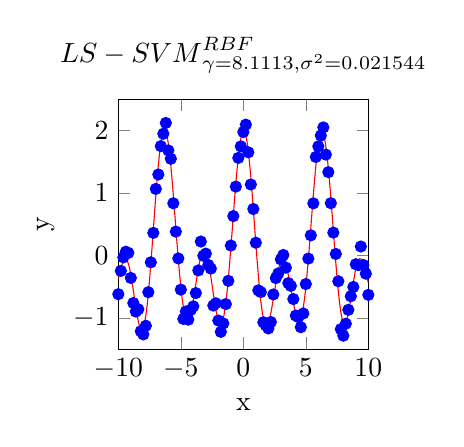
\begin{tikzpicture}

\begin{axis}[%
width=1.25in,
height=1.25in,
scale only axis,
xmin=-10,
xmax=10,
xlabel={x},
ymin=-1.5,
ymax=2.5,
ylabel={y},
title={$\text{LS-SVM}_{\gamma\text{=8.1113,}\sigma{}^\text{2}\text{=0.021544}}^{\text{RBF}}$}
]
\addplot [color=red,solid,forget plot]
  table[row sep=crcr]{%
-10	-0.378155848083547\\
-9.9	-0.294876235938143\\
-9.8	-0.216122205479947\\
-9.7	-0.147876896762239\\
-9.6	-0.0958533699641556\\
-9.5	-0.065043342605781\\
-9.4	-0.0592979764652931\\
-9.3	-0.0809783616834283\\
-9.2	-0.130707121849832\\
-9.1	-0.207243091621335\\
-9	-0.307489519593927\\
-8.9	-0.426634148743443\\
-8.8	-0.558408229639226\\
-8.7	-0.695442210023953\\
-8.6	-0.829689331359161\\
-8.5	-0.952885023239864\\
-8.4	-1.05700976735817\\
-8.3	-1.1347256011633\\
-8.2	-1.17976101320801\\
-8.1	-1.18722491088169\\
-8	-1.1538368915467\\
-7.9	-1.0780675861544\\
-7.8	-0.96018886919266\\
-7.7	-0.802238880544155\\
-7.6	-0.607910853023286\\
-7.5	-0.382377564765225\\
-7.4	-0.13206481668019\\
-7.3	0.135612257220494\\
-7.2	0.412536841558149\\
-7.1	0.690190209721806\\
-7	0.959953564980523\\
-6.9	1.21340377490603\\
-6.8	1.4425964183712\\
-6.7	1.64033061897014\\
-6.6	1.80039051577865\\
-6.5	1.91775795867774\\
-6.4	1.98879032430155\\
-6.3	2.0113565857991\\
-6.2	1.98492436370741\\
-6.1	1.91059104569894\\
-6	1.7910534839738\\
-5.9	1.63051336157977\\
-5.8	1.43451892897771\\
-5.7	1.20974808656245\\
-5.6	0.963742189612541\\
-5.5	0.704603859930663\\
-5.4	0.44067491704934\\
-5.3	0.180211850852144\\
-5.2	-0.0689241602108382\\
-5.1	-0.299547754445033\\
-5	-0.505388873190403\\
-4.9	-0.681283838984376\\
-4.8	-0.823314897917623\\
-4.7	-0.928898825775779\\
-4.6	-0.996827884395797\\
-4.5	-1.02726778403292\\
-4.4	-1.02171735999765\\
-4.3	-0.982933678397346\\
-4.2	-0.914824726648321\\
-4.1	-0.822310305536334\\
-4	-0.711150788793284\\
-3.9	-0.587743483440506\\
-3.8	-0.458887611334805\\
-3.7	-0.331521370033481\\
-3.6	-0.212437791196766\\
-3.5	-0.107989674853166\\
-3.4	-0.0237971226056478\\
-3.3	0.0355264696830814\\
-3.2	0.0666131305368795\\
-3.1	0.067527568285264\\
-3	0.037889080832013\\
-2.9	-0.0210820461907696\\
-2.8	-0.106599067349452\\
-2.7	-0.214424350155148\\
-2.6	-0.339060784151469\\
-2.5	-0.474008925856841\\
-2.4	-0.612075697524962\\
-2.3	-0.745717450838724\\
-2.2	-0.867398429866311\\
-2.1	-0.969945182007542\\
-2	-1.04687825474257\\
-1.9	-1.09270449604647\\
-1.8	-1.10315629752684\\
-1.7	-1.07536796038565\\
-1.6	-1.00798372814477\\
-1.5	-0.901196549991163\\
-1.4	-0.756720902216105\\
-1.3	-0.577706588810396\\
-1.2	-0.368603010833183\\
-1.1	-0.134984706147812\\
-1	0.116651037628226\\
-0.9	0.379104852812625\\
-0.799999999999999	0.644706573224734\\
-0.699999999999999	0.905551757004319\\
-0.6	1.15374016324667\\
-0.5	1.38161426804077\\
-0.399999999999999	1.58199622928933\\
-0.299999999999999	1.74842087713643\\
-0.199999999999999	1.87536047567285\\
-0.0999999999999996	1.95843457253841\\
0	1.9945957951916\\
0.0999999999999996	1.98228059037254\\
0.199999999999999	1.92151318818227\\
0.299999999999999	1.81395186710705\\
0.399999999999999	1.6628689972473\\
0.5	1.47306015170144\\
0.6	1.25068235225715\\
0.699999999999999	1.00302664067485\\
0.799999999999999	0.738234979177406\\
0.9	0.464975398555039\\
1	0.19209192381836\\
1.1	-0.0717530526508091\\
1.2	-0.318426538420568\\
1.3	-0.540646824919553\\
1.4	-0.73226560595447\\
1.5	-0.888498959718327\\
1.6	-1.00609840016916\\
1.7	-1.08345568420302\\
1.8	-1.12063743616203\\
1.9	-1.11934803268286\\
2	-1.08282174273582\\
2.1	-1.0156479716616\\
2.2	-0.923536636461624\\
2.3	-0.813034067688702\\
2.4	-0.691203094567072\\
2.5	-0.565283708979081\\
2.6	-0.442352467372367\\
2.7	-0.328999187767102\\
2.8	-0.231038303755436\\
2.9	-0.153269452796243\\
3	-0.0992977638493906\\
3.1	-0.0714193604237752\\
3.2	-0.0705724519125292\\
3.3	-0.0963497302985599\\
3.4	-0.147064217728661\\
3.5	-0.219858625081448\\
3.6	-0.310847816643414\\
3.7	-0.415284976460339\\
3.8	-0.527744128613192\\
3.9	-0.642314196059252\\
4	-0.752802153103253\\
4.1	-0.852944462395901\\
4.2	-0.936626487620834\\
4.3	-0.998108779872837\\
4.4	-1.03225715920071\\
4.5	-1.03477070694114\\
4.6	-1.00239868198467\\
4.7	-0.933134593399615\\
4.8	-0.826373803915961\\
4.9	-0.683020590901011\\
5	-0.50553185119428\\
5.1	-0.297887664656759\\
5.2	-0.0654835394487272\\
5.3	0.185055070977024\\
5.4	0.446129068930357\\
5.5	0.709479767658797\\
5.6	0.966542396608503\\
5.7	1.20881710445227\\
5.8	1.42823396519454\\
5.9	1.61748932296474\\
6	1.77033397543138\\
6.1	1.88179882980166\\
6.2	1.94835010653516\\
6.3	1.96797303199366\\
6.4	1.94018927507218\\
6.5	1.86601822733625\\
6.6	1.74789490548876\\
6.7	1.58955743151702\\
6.8	1.39591482366046\\
6.9	1.17290176319979\\
7	0.927322011308792\\
7.1	0.666677374720198\\
7.2	0.398975702504972\\
7.3	0.132510265317376\\
7.4	-0.124395461506011\\
7.5	-0.363679137594506\\
7.6	-0.577861891395248\\
7.7	-0.760388718502137\\
7.8	-0.905966427432029\\
7.9	-1.01087266836014\\
8	-1.07320651161869\\
8.1	-1.09305168336255\\
8.2	-1.07252818913541\\
8.3	-1.01571632761261\\
8.4	-0.928448126531717\\
8.5	-0.817973716505258\\
8.6	-0.692522577921945\\
8.7	-0.560790441156105\\
8.8	-0.431390593964865\\
8.9	-0.312312528703424\\
9	-0.210430791627665\\
9.1	-0.131102619710374\\
9.2	-0.0778849716734599\\
9.3	-0.0523907623848497\\
9.4	-0.054291639277566\\
9.5	-0.0814617731758166\\
9.6	-0.130245148220669\\
9.7	-0.195818872156336\\
9.8	-0.272617996960495\\
9.9	-0.354783825863167\\
10	-0.436597895179934\\
};
\addplot [color=blue,only marks,mark=*,mark options={solid},forget plot]
  table[row sep=crcr]{%
-10	-0.619595049893259\\
-9.8	-0.247437337833684\\
-9.6	-0.0306624145407526\\
-9.4	0.0595016992990417\\
-9.2	0.0405503353753764\\
-9	-0.359577760153356\\
-8.8	-0.761497412492202\\
-8.6	-0.897663190767661\\
-8.4	-0.860637115262312\\
-8.2	-1.2126167956593\\
-8	-1.26313692928078\\
-7.8	-1.12516839132702\\
-7.6	-0.588065125145126\\
-7.4	-0.109694576560566\\
-7.2	0.361280183367072\\
-7	1.0646759786683\\
-6.8	1.29538129968242\\
-6.6	1.74884224001031\\
-6.4	1.94683351065395\\
-6.2	2.11982365358625\\
-6	1.68022816856692\\
-5.8	1.54627677608122\\
-5.6	0.834565398848264\\
-5.4	0.381366445534563\\
-5.2	-0.0478095833588603\\
-5	-0.546903359444873\\
-4.8	-1.01522643475883\\
-4.6	-0.897166537197328\\
-4.4	-1.02680658292176\\
-4.2	-0.871089932079635\\
-4	-0.814155649020787\\
-3.8	-0.60175571130384\\
-3.6	-0.238907143455007\\
-3.4	0.222208137340781\\
-3.2	-0.00492514934068313\\
-3	0.0292466251038767\\
-2.8	-0.152773332407692\\
-2.6	-0.210247299070627\\
-2.4	-0.801924853922079\\
-2.2	-0.765333121147812\\
-2	-1.04175373212827\\
-1.8	-1.22268061922734\\
-1.6	-1.08813837606648\\
-1.4	-0.778398776369186\\
-1.2	-0.406010477529214\\
-1	0.158410672742104\\
-0.799999999999999	0.629656009659678\\
-0.6	1.1012539129474\\
-0.399999999999999	1.56095744357927\\
-0.199999999999999	1.74538482106182\\
0	1.97514838527262\\
0.199999999999999	2.09333728242314\\
0.399999999999999	1.65001281210317\\
0.6	1.13516770216898\\
0.799999999999999	0.742729092315044\\
1	0.203344072966865\\
1.2	-0.558470765447578\\
1.4	-0.586110482986666\\
1.6	-1.06883931097022\\
1.8	-1.11741980461136\\
2	-1.16758084046331\\
2.2	-1.06511621288888\\
2.4	-0.623929796601062\\
2.6	-0.362230376187371\\
2.8	-0.286628861691811\\
3	-0.0622448540645585\\
3.2	0.00790495738628174\\
3.4	-0.194949615007405\\
3.6	-0.442522817019591\\
3.8	-0.486757328807435\\
4	-0.69787996654234\\
4.2	-0.962269330093291\\
4.4	-0.985769144108822\\
4.6	-1.14773117213016\\
4.8	-0.92842012618687\\
5	-0.457544358332057\\
5.2	-0.0501283831683725\\
5.4	0.321923931056346\\
5.6	0.833778247649155\\
5.8	1.5757751546434\\
6	1.74494490112986\\
6.2	1.91809847491895\\
6.4	2.04847928009022\\
6.6	1.61361768813205\\
6.8	1.33288010477131\\
7	0.836064061458198\\
7.2	0.365373991683923\\
7.4	0.0243115018755421\\
7.6	-0.412557611585228\\
7.8	-1.17965097458037\\
8	-1.28369946344995\\
8.2	-1.09154240409875\\
8.4	-0.869970337849687\\
8.6	-0.652727819002938\\
8.8	-0.504839095267686\\
9	-0.140625208970404\\
9.2	-0.155007196552229\\
9.4	0.142883162331669\\
9.6	-0.152697183256788\\
9.8	-0.291450155475497\\
10	-0.630494381710576\\
};
\end{axis}
\end{tikzpicture}%
\end{document}
% This file was created by matlab2tikz.
% Minimal pgfplots version: 1.3
%
%The latest updates can be retrieved from
%  http://www.mathworks.com/matlabcentral/fileexchange/22022-matlab2tikz
%where you can also make suggestions and rate matlab2tikz.
%
\documentclass[tikz]{standalone}
\usepackage{pgfplots}
\usepackage{grffile}
\pgfplotsset{compat=newest}
\usetikzlibrary{plotmarks}
\usepackage{amsmath}

\begin{document}
\definecolor{mycolor1}{rgb}{0.00000,0.44700,0.74100}%
\definecolor{mycolor2}{rgb}{0.85000,0.32500,0.09800}%
%
\begin{tikzpicture}

\begin{axis}[%
width=1.25in,
height=1.25in,
scale only axis,
xmin=-10,
xmax=10,
ymin=-1.5,
ymax=2.5,
xlabel={x},
ylabel={y},
legend style={legend cell align=left,align=left,draw=white!15!black}
]
\addplot [color=mycolor1,only marks,mark=*,mark options={solid}]
  table[row sep=crcr]{%
-9.9	-0.446457785387605\\
-9.7	0.0615741857353768\\
-9.5	-0.0899003134505097\\
-9.3	0.00653549107191894\\
-9.1	-0.233751653584901\\
-8.9	-0.291859160079753\\
-8.7	-0.613731475283965\\
-8.5	-1.03528169296305\\
-8.3	-0.9642330834576\\
-8.1	-1.27978596939285\\
-7.9	-0.986978063124592\\
-7.7	-0.941541670603769\\
-7.5	-0.424284871548671\\
-7.3	0.0024000252430941\\
-7.1	0.612256274995885\\
-6.9	1.10201532421862\\
-6.7	1.60211115914485\\
-6.5	1.76220978074123\\
-6.3	1.99979524181867\\
-6.1	1.79034879732083\\
-5.9	1.44403094330746\\
-5.7	1.29383877713738\\
-5.5	0.613830121265493\\
-5.3	0.100331531211364\\
-5.1	-0.325372368531793\\
-4.9	-0.64567925384688\\
-4.7	-0.96024547762059\\
-4.5	-1.07928199677673\\
-4.3	-0.972498020860962\\
-4.1	-1.02965915981306\\
-3.9	-0.755152776972108\\
-3.7	-0.589677281173566\\
-3.5	-0.166490277986134\\
-3.3	0.0236256253118752\\
-3.1	-0.22676123328907\\
-2.9	-0.23110988817597\\
-2.7	-0.200813017281912\\
-2.5	-0.491113134760776\\
-2.3	-0.84073572657711\\
-2.1	-0.985056993540881\\
-1.9	-1.05132963955875\\
-1.7	-1.15426680135552\\
-1.5	-0.779866365644407\\
-1.3	-0.688580620762527\\
-1.1	-0.0433129495232868\\
-0.9	0.508987303868705\\
-0.699999999999999	0.697600560057975\\
-0.5	1.42603297588922\\
-0.299999999999999	1.89054346075414\\
-0.0999999999999996	1.99857339590222\\
0.0999999999999996	1.70788159322484\\
0.299999999999999	1.6759300758617\\
0.5	1.49638851300071\\
0.699999999999999	1.04119258285231\\
0.9	0.301598925511327\\
1.1	-0.159278370503842\\
1.3	-0.529632069442699\\
1.5	-0.869771393788035\\
1.7	-1.20941576364803\\
1.9	-1.18707415269971\\
2.1	-1.05532322902962\\
2.3	-0.797889105745886\\
2.5	-0.498836517243156\\
2.7	-0.370696460770287\\
2.9	-0.212410851613561\\
3.1	-0.0759893540469849\\
3.3	0.202379146677431\\
3.5	-0.15504532673161\\
3.7	-0.455920196582363\\
3.9	-0.883007950496145\\
4.1	-0.798073602984103\\
4.3	-1.15799842570728\\
4.5	-1.10879202963167\\
4.7	-1.14475761549896\\
4.9	-0.718500284867997\\
5.1	-0.399271702450803\\
5.3	0.0633190838576606\\
5.5	0.828518914985831\\
5.7	1.31722910868865\\
5.9	1.60141103275897\\
6.1	1.7846292176811\\
6.3	2.07597483058294\\
6.5	1.86948734102912\\
6.7	1.5439487097687\\
6.9	1.0778203170723\\
7.1	0.804338148231601\\
7.3	0.0295045907637691\\
7.5	-0.390997298935905\\
7.7	-0.677198469150053\\
7.9	-1.21318786763014\\
8.1	-1.22754939070245\\
8.3	-1.03150807115426\\
8.5	-0.948758708294413\\
8.7	-0.612207588633159\\
8.9	-0.342665934347301\\
9.1	-0.184215026650319\\
9.3	-0.0609189088953476\\
9.5	0.0628781633101973\\
9.7	-0.0694799394785849\\
9.9	-0.153493005615711\\
};

\addplot [color=mycolor2,only marks,mark=+,mark options={solid}]
  table[row sep=crcr]{%
-9.9	-0.294876235938143\\
-9.7	-0.147876896762239\\
-9.5	-0.065043342605781\\
-9.3	-0.0809783616834283\\
-9.1	-0.207243091621335\\
-8.9	-0.426634148743443\\
-8.7	-0.695442210023953\\
-8.5	-0.952885023239864\\
-8.3	-1.1347256011633\\
-8.1	-1.18722491088169\\
-7.9	-1.0780675861544\\
-7.7	-0.802238880544155\\
-7.5	-0.382377564765225\\
-7.3	0.135612257220494\\
-7.1	0.690190209721806\\
-6.9	1.21340377490603\\
-6.7	1.64033061897014\\
-6.5	1.91775795867774\\
-6.3	2.0113565857991\\
-6.1	1.91059104569894\\
-5.9	1.63051336157977\\
-5.7	1.20974808656245\\
-5.5	0.704603859930663\\
-5.3	0.180211850852144\\
-5.1	-0.299547754445033\\
-4.9	-0.681283838984376\\
-4.7	-0.928898825775779\\
-4.5	-1.02726778403292\\
-4.3	-0.982933678397346\\
-4.1	-0.822310305536334\\
-3.9	-0.587743483440506\\
-3.7	-0.331521370033481\\
-3.5	-0.107989674853166\\
-3.3	0.0355264696830814\\
-3.1	0.067527568285264\\
-2.9	-0.0210820461907696\\
-2.7	-0.214424350155148\\
-2.5	-0.474008925856841\\
-2.3	-0.745717450838724\\
-2.1	-0.969945182007542\\
-1.9	-1.09270449604647\\
-1.7	-1.07536796038565\\
-1.5	-0.901196549991163\\
-1.3	-0.577706588810396\\
-1.1	-0.134984706147812\\
-0.9	0.379104852812625\\
-0.699999999999999	0.905551757004319\\
-0.5	1.38161426804077\\
-0.299999999999999	1.74842087713643\\
-0.0999999999999996	1.95843457253841\\
0.0999999999999996	1.98228059037254\\
0.299999999999999	1.81395186710705\\
0.5	1.47306015170144\\
0.699999999999999	1.00302664067485\\
0.9	0.464975398555039\\
1.1	-0.0717530526508091\\
1.3	-0.540646824919553\\
1.5	-0.888498959718327\\
1.7	-1.08345568420302\\
1.9	-1.11934803268286\\
2.1	-1.0156479716616\\
2.3	-0.813034067688702\\
2.5	-0.565283708979081\\
2.7	-0.328999187767102\\
2.9	-0.153269452796243\\
3.1	-0.0714193604237752\\
3.3	-0.0963497302985599\\
3.5	-0.219858625081448\\
3.7	-0.415284976460339\\
3.9	-0.642314196059252\\
4.1	-0.852944462395901\\
4.3	-0.998108779872837\\
4.5	-1.03477070694114\\
4.7	-0.933134593399615\\
4.9	-0.683020590901011\\
5.1	-0.297887664656759\\
5.3	0.185055070977024\\
5.5	0.709479767658797\\
5.7	1.20881710445227\\
5.9	1.61748932296474\\
6.1	1.88179882980166\\
6.3	1.96797303199366\\
6.5	1.86601822733625\\
6.7	1.58955743151702\\
6.9	1.17290176319979\\
7.1	0.666677374720198\\
7.3	0.132510265317376\\
7.5	-0.363679137594506\\
7.7	-0.760388718502137\\
7.9	-1.01087266836014\\
8.1	-1.09305168336255\\
8.3	-1.01571632761261\\
8.5	-0.817973716505258\\
8.7	-0.560790441156105\\
8.9	-0.312312528703424\\
9.1	-0.131102619710374\\
9.3	-0.0523907623848497\\
9.5	-0.0814617731758166\\
9.7	-0.195818872156336\\
9.9	-0.354783825863167\\
};

\end{axis}
\end{tikzpicture}%
\end{document}
% This file was created by matlab2tikz.
% Minimal pgfplots version: 1.3
%
%The latest updates can be retrieved from
%  http://www.mathworks.com/matlabcentral/fileexchange/22022-matlab2tikz
%where you can also make suggestions and rate matlab2tikz.
%
\documentclass[tikz]{standalone}
\usepackage{pgfplots}
\usepackage{grffile}
\pgfplotsset{compat=newest}
\usetikzlibrary{plotmarks}
\usepackage{amsmath}

\begin{document}
\begin{tikzpicture}

\begin{axis}[%
width=1.25in,
height=1.25in,
scale only axis,
xmin=-5,
xmax=0,
xlabel={$\sigma^2$},
xmajorgrids,
ymin=0,
ymax=10,
ylabel={$\gamma$},
ymajorgrids,
zmin=0,
zmax=10,
zmajorgrids,
view={90}{90},
axis x line*=bottom,
axis y line*=left,
axis z line*=left
]

\addplot3[%
surf,
shader=flat,
colormap={mymap}{[1pt] rgb(0pt)=(0.2081,0.1663,0.5292); rgb(1pt)=(0.211624,0.189781,0.577676); rgb(2pt)=(0.212252,0.213771,0.626971); rgb(3pt)=(0.2081,0.2386,0.677086); rgb(4pt)=(0.195905,0.264457,0.7279); rgb(5pt)=(0.170729,0.291938,0.779248); rgb(6pt)=(0.125271,0.324243,0.830271); rgb(7pt)=(0.0591333,0.359833,0.868333); rgb(8pt)=(0.0116952,0.38751,0.881957); rgb(9pt)=(0.00595714,0.408614,0.882843); rgb(10pt)=(0.0165143,0.4266,0.878633); rgb(11pt)=(0.0328524,0.443043,0.871957); rgb(12pt)=(0.0498143,0.458571,0.864057); rgb(13pt)=(0.0629333,0.47369,0.855438); rgb(14pt)=(0.0722667,0.488667,0.8467); rgb(15pt)=(0.0779429,0.503986,0.838371); rgb(16pt)=(0.0793476,0.520024,0.831181); rgb(17pt)=(0.0749429,0.537543,0.826271); rgb(18pt)=(0.0640571,0.556986,0.823957); rgb(19pt)=(0.0487714,0.577224,0.822829); rgb(20pt)=(0.0343429,0.596581,0.819852); rgb(21pt)=(0.0265,0.6137,0.8135); rgb(22pt)=(0.0238905,0.628662,0.803762); rgb(23pt)=(0.0230905,0.641786,0.791267); rgb(24pt)=(0.0227714,0.653486,0.776757); rgb(25pt)=(0.0266619,0.664195,0.760719); rgb(26pt)=(0.0383714,0.674271,0.743552); rgb(27pt)=(0.0589714,0.683757,0.725386); rgb(28pt)=(0.0843,0.692833,0.706167); rgb(29pt)=(0.113295,0.7015,0.685857); rgb(30pt)=(0.145271,0.709757,0.664629); rgb(31pt)=(0.180133,0.717657,0.642433); rgb(32pt)=(0.217829,0.725043,0.619262); rgb(33pt)=(0.258643,0.731714,0.595429); rgb(34pt)=(0.302171,0.737605,0.571186); rgb(35pt)=(0.348167,0.742433,0.547267); rgb(36pt)=(0.395257,0.7459,0.524443); rgb(37pt)=(0.44201,0.748081,0.503314); rgb(38pt)=(0.487124,0.749062,0.483976); rgb(39pt)=(0.530029,0.749114,0.466114); rgb(40pt)=(0.570857,0.748519,0.44939); rgb(41pt)=(0.609852,0.747314,0.433686); rgb(42pt)=(0.6473,0.7456,0.4188); rgb(43pt)=(0.683419,0.743476,0.404433); rgb(44pt)=(0.71841,0.741133,0.390476); rgb(45pt)=(0.752486,0.7384,0.376814); rgb(46pt)=(0.785843,0.735567,0.363271); rgb(47pt)=(0.818505,0.732733,0.34979); rgb(48pt)=(0.850657,0.7299,0.336029); rgb(49pt)=(0.882433,0.727433,0.3217); rgb(50pt)=(0.913933,0.725786,0.306276); rgb(51pt)=(0.944957,0.726114,0.288643); rgb(52pt)=(0.973895,0.731395,0.266648); rgb(53pt)=(0.993771,0.745457,0.240348); rgb(54pt)=(0.999043,0.765314,0.216414); rgb(55pt)=(0.995533,0.786057,0.196652); rgb(56pt)=(0.988,0.8066,0.179367); rgb(57pt)=(0.978857,0.827143,0.163314); rgb(58pt)=(0.9697,0.848138,0.147452); rgb(59pt)=(0.962586,0.870514,0.1309); rgb(60pt)=(0.958871,0.8949,0.113243); rgb(61pt)=(0.959824,0.921833,0.0948381); rgb(62pt)=(0.9661,0.951443,0.0755333); rgb(63pt)=(0.9763,0.9831,0.0538)},
mesh/rows=100]
table[row sep=crcr,header=false] {%
%
-5	0	9.71142221677984\\
-5	0.101010101010101	9.71140389779787\\
-5	0.202020202020202	9.71133157748906\\
-5	0.303030303030303	9.71108866364165\\
-5	0.404040404040404	9.71038231696047\\
-5	0.505050505050505	9.70857639673274\\
-5	0.606060606060606	9.70445997701801\\
-5	0.707070707070707	9.69599033644247\\
-5	0.808080808080808	9.68008498106293\\
-5	0.909090909090909	9.65255230147744\\
-5	1.01010101010101	9.60823099716993\\
-5	1.11111111111111	9.54135739289275\\
-5	1.21212121212121	9.44611626222461\\
-5	1.31313131313131	9.31727946697319\\
-5	1.41414141414141	9.15081579818331\\
-5	1.51515151515152	8.94436985684349\\
-5	1.61616161616162	8.69755000378289\\
-5	1.71717171717172	8.41201953179298\\
-5	1.81818181818182	8.0914319996519\\
-5	1.91919191919192	7.74127308928682\\
-5	2.02020202020202	7.36865697285339\\
-5	2.12121212121212	6.98207929813651\\
-5	2.22222222222222	6.59107386107618\\
-5	2.32323232323232	6.20569089073058\\
-5	2.42424242424242	5.83574370568315\\
-5	2.52525252525253	5.48986433431911\\
-5	2.62626262626263	5.17453335022118\\
-5	2.72727272727273	4.89333662120591\\
-5	2.82828282828283	4.64668763180221\\
-5	2.92929292929293	4.43212530463919\\
-5	3.03030303030303	4.24510923332891\\
-5	3.13131313131313	4.08007813894372\\
-5	3.23232323232323	3.93148179992769\\
-5	3.33333333333333	3.79455148521732\\
-5	3.43434343434343	3.66569731720236\\
-5	3.53535353535354	3.54255252096777\\
-5	3.63636363636364	3.42377535273262\\
-5	3.73737373737374	3.30874825928866\\
-5	3.83838383838384	3.19728824561706\\
-5	3.93939393939394	3.08942972027933\\
-5	4.04040404040404	2.98529117204018\\
-5	4.14141414141414	2.88500760942979\\
-5	4.24242424242424	2.7887029600321\\
-5	4.34343434343434	2.69648196820019\\
-5	4.44444444444444	2.60843039263769\\
-5	4.54545454545455	2.52461997905935\\
-5	4.64646464646465	2.44511830184894\\
-5	4.74747474747475	2.37000278952208\\
-5	4.84848484848485	2.29937513088621\\
-5	4.94949494949495	2.23337054344156\\
-5	5.05050505050505	2.17215862952682\\
-5	5.15151515151515	2.11593761748802\\
-5	5.25252525252525	2.0649278213709\\
-5	5.35353535353535	2.01937036709782\\
-5	5.45454545454545	1.97953458705286\\
-5	5.55555555555556	1.94573519074472\\
-5	5.65656565656566	1.91835994277943\\
-5	5.75757575757576	1.8979088670444\\
-5	5.85858585858586	1.88504540661013\\
-5	5.95959595959596	1.88065819624512\\
-5	6.06060606060606	1.88592995845182\\
-5	6.16161616161616	1.90241064246018\\
-5	6.26262626262626	1.9320985452317\\
-5	6.36363636363636	1.97754138993487\\
-5	6.46464646464646	2.04196706625944\\
-5	6.56565656565657	2.1294342344993\\
-5	6.66666666666667	2.24496291455581\\
-5	6.76767676767677	2.39457352575721\\
-5	6.86868686868687	2.58512511060784\\
-5	6.96969696969697	2.82378869281159\\
-5	7.07070707070707	3.11693714371589\\
-5	7.17171717171717	3.46825403441113\\
-5	7.27272727272727	3.87609364592065\\
-5	7.37373737373737	4.33068823175355\\
-5	7.47474747474747	4.81258912661282\\
-5	7.57575757575758	5.29411277134777\\
-5	7.67676767676768	5.74466615932254\\
-5	7.77777777777778	6.1386580399485\\
-5	7.87878787878788	6.46268248672824\\
-5	7.97979797979798	6.71848722691886\\
-5	8.08080808080808	6.92046177476854\\
-5	8.18181818181818	7.08967133544705\\
-5	8.28282828282828	7.24803947536821\\
-5	8.38383838383838	7.41463350493836\\
-5	8.48484848484848	7.60328127105507\\
-5	8.58585858585859	7.82033916154883\\
-5	8.68686868686869	8.06332431777104\\
-5	8.78787878787879	8.3220094751847\\
-5	8.88888888888889	8.58185903084134\\
-5	8.98989898989899	8.82781708099047\\
-5	9.09090909090909	9.04692345740679\\
-5	9.19191919191919	9.22989559098724\\
-5	9.29292929292929	9.3722784283822\\
-5	9.39393939393939	9.47495304520139\\
-5	9.49494949494949	9.54339029446297\\
-5	9.5959595959596	9.58572657183269\\
-5	9.6969696969697	9.61054080474783\\
-5	9.7979797979798	9.62520371347509\\
-5	9.8989898989899	9.63509098847121\\
-5	10	9.64348641937173\\
-4.94949494949495	0	9.71142167926959\\
-4.94949494949495	0.101010101010101	9.71140123948528\\
-4.94949494949495	0.202020202020202	9.71132054660067\\
-4.94949494949495	0.303030303030303	9.71104951044657\\
-4.94949494949495	0.404040404040404	9.71026138959856\\
-4.94949494949495	0.505050505050505	9.70824639750565\\
-4.94949494949495	0.606060606060606	9.70365342186232\\
-4.94949494949495	0.707070707070707	9.69420326857134\\
-4.94949494949495	0.808080808080808	9.67645663259656\\
-4.94949494949495	0.909090909090909	9.64573679145825\\
-4.94949494949495	1.01010101010101	9.59628530601474\\
-4.94949494949495	1.11111111111111	9.52167210570779\\
-4.94949494949495	1.21212121212121	9.41541047427978\\
-4.94949494949495	1.31313131313131	9.27167022464262\\
-4.94949494949495	1.41414141414141	9.08595911475644\\
-4.94949494949495	1.51515151515152	8.85565901346967\\
-4.94949494949495	1.61616161616162	8.58035107999663\\
-4.94949494949495	1.71717171717172	8.26192551433383\\
-4.94949494949495	1.81818181818182	7.90452410458374\\
-4.94949494949495	1.91919191919192	7.51438654115999\\
-4.94949494949495	2.02020202020202	7.0996516222492\\
-4.94949494949495	2.12121212121212	6.67010710495475\\
-4.94949494949495	2.22222222222222	6.2368144501488\\
-4.94949494949495	2.32323232323232	5.81150061203663\\
-4.94949494949495	2.42424242424242	5.40564862921429\\
-4.94949494949495	2.52525252525253	5.0293408896816\\
-4.94949494949495	2.62626262626263	4.69006926222821\\
-4.94949494949495	2.72727272727273	4.39183586154036\\
-4.94949494949495	2.82828282828283	4.13484309383091\\
-4.94949494949495	2.92929292929293	3.91589759875969\\
-4.94949494949495	3.03030303030303	3.72940929941481\\
-4.94949494949495	3.13131313131313	3.56867815139841\\
-4.94949494949495	3.23232323232323	3.42711129047998\\
-4.94949494949495	3.33333333333333	3.29910031912854\\
-4.94949494949495	3.43434343434343	3.18044735504394\\
-4.94949494949495	3.53535353535354	3.06838260582747\\
-4.94949494949495	3.63636363636364	2.96131347086355\\
-4.94949494949495	3.73737373737374	2.85846859127728\\
-4.94949494949495	3.83838383838384	2.75956424499123\\
-4.94949494949495	3.93939393939394	2.66455798115544\\
-4.94949494949495	4.04040404040404	2.57349861728354\\
-4.94949494949495	4.14141414141414	2.48645051966548\\
-4.94949494949495	4.24242424242424	2.40346267272872\\
-4.94949494949495	4.34343434343434	2.32455912594137\\
-4.94949494949495	4.44444444444444	2.24973781869955\\
-4.94949494949495	4.54545454545455	2.17897444802103\\
-4.94949494949495	4.64646464646465	2.11223348696236\\
-4.94949494949495	4.74747474747475	2.04948735615473\\
-4.94949494949495	4.84848484848485	1.99073875889208\\
-4.94949494949495	4.94949494949495	1.93603652701466\\
-4.94949494949495	5.05050505050505	1.88547768913874\\
-4.94949494949495	5.15151515151515	1.83919701420085\\
-4.94949494949495	5.25252525252525	1.79735295563202\\
-4.94949494949495	5.35353535353535	1.76011955550373\\
-4.94949494949495	5.45454545454545	1.72768850749617\\
-4.94949494949495	5.55555555555556	1.70028095650879\\
-4.94949494949495	5.65656565656566	1.67816897424019\\
-4.94949494949495	5.75757575757576	1.66170938774762\\
-4.94949494949495	5.85858585858586	1.6513935043361\\
-4.94949494949495	5.95959595959596	1.64791398445157\\
-4.94949494949495	6.06060606060606	1.65224472704423\\
-4.94949494949495	6.16161616161616	1.66572511709204\\
-4.94949494949495	6.26262626262626	1.69014602761138\\
-4.94949494949495	6.36363636363636	1.72785240715437\\
-4.94949494949495	6.46464646464646	1.78188735013213\\
-4.94949494949495	6.56565656565657	1.85618624370098\\
-4.94949494949495	6.66666666666667	1.95579174725998\\
-4.94949494949495	6.76767676767677	2.08702104609988\\
-4.94949494949495	6.86868686868687	2.25747909494098\\
-4.94949494949495	6.96969696969697	2.47575095474901\\
-4.94949494949495	7.07070707070707	2.75051357026197\\
-4.94949494949495	7.17171717171717	3.08874494239786\\
-4.94949494949495	7.27272727272727	3.49282919494749\\
-4.94949494949495	7.37373737373737	3.95688315816791\\
-4.94949494949495	7.47474747474747	4.46366456236852\\
-4.94949494949495	7.57575757575758	4.98441392518124\\
-4.94949494949495	7.67676767676768	5.4835770422405\\
-4.94949494949495	7.77777777777778	5.92784674631657\\
-4.94949494949495	7.87878787878788	6.29588498128486\\
-4.94949494949495	7.97979797979798	6.58395937428513\\
-4.94949494949495	8.08080808080808	6.80473062566524\\
-4.94949494949495	8.18181818181818	6.98061837615216\\
-4.94949494949495	8.28282828282828	7.13635993918139\\
-4.94949494949495	8.38383838383838	7.29433669600206\\
-4.94949494949495	8.48484848484848	7.47221753174323\\
-4.94949494949495	8.58585858585859	7.68055240248904\\
-4.94949494949495	8.68686868686869	7.92025187553388\\
-4.94949494949495	8.78787878787879	8.18247699547346\\
-4.94949494949495	8.88888888888889	8.45213493813682\\
-4.94949494949495	8.98989898989899	8.71276515824471\\
-4.94949494949495	9.09090909090909	8.94994866268236\\
-4.94949494949495	9.19191919191919	9.15280818127921\\
-4.94949494949495	9.29292929292929	9.31489132876324\\
-4.94949494949495	9.39393939393939	9.43497492753353\\
-4.94949494949495	9.49494949494949	9.51702075432333\\
-4.94949494949495	9.5959595959596	9.56869339834603\\
-4.94949494949495	9.6969696969697	9.59902583698428\\
-4.94949494949495	9.7979797979798	9.61634990417677\\
-4.94949494949495	9.8989898989899	9.6271213478953\\
-4.94949494949495	10	9.63558666025153\\
-4.8989898989899	0	9.71142115597714\\
-4.8989898989899	0.101010101010101	9.7113986514883\\
-4.8989898989899	0.202020202020202	9.71130980749288\\
-4.8989898989899	0.303030303030303	9.7110113929039\\
-4.8989898989899	0.404040404040404	9.7101436609396\\
-4.8989898989899	0.505050505050505	9.70792512736293\\
-4.8989898989899	0.606060606060606	9.702868202291\\
-4.8989898989899	0.707070707070707	9.6924634768283\\
-4.8989898989899	0.808080808080808	9.67292428327859\\
-4.8989898989899	0.909090909090909	9.63910164875787\\
-4.8989898989899	1.01010101010101	9.58465587001585\\
-4.8989898989899	1.11111111111111	9.50250828914412\\
-4.8989898989899	1.21212121212121	9.38551883486359\\
-4.8989898989899	1.31313131313131	9.22727191171258\\
-4.8989898989899	1.41414141414141	9.02282775994852\\
-4.8989898989899	1.51515151515152	8.76931489581012\\
-4.8989898989899	1.61616161616162	8.46629256379988\\
-4.8989898989899	1.71717171717172	8.11588060542613\\
-4.8989898989899	1.81818181818182	7.72271264876739\\
-4.8989898989899	1.91919191919192	7.29379229846441\\
-4.8989898989899	2.02020202020202	6.83830594222351\\
-4.8989898989899	2.12121212121212	6.36737566103727\\
-4.8989898989899	2.22222222222222	5.89365428089877\\
-4.8989898989899	2.32323232323232	5.43062472244378\\
-4.8989898989899	2.42424242424242	4.99151731014569\\
-4.8989898989899	2.52525252525253	4.58791332947794\\
-4.8989898989899	2.62626262626263	4.22830603995841\\
-4.8989898989899	2.72727272727273	3.91702817487881\\
-4.8989898989899	2.82828282828283	3.65391775839005\\
-4.8989898989899	2.92929292929293	3.43486286096809\\
-4.8989898989899	3.03030303030303	3.25305057514249\\
-4.8989898989899	3.13131313131313	3.10051718135014\\
-4.8989898989899	3.23232323232323	2.9695612412471\\
-4.8989898989899	3.33333333333333	2.85371676368859\\
-4.8989898989899	3.43434343434343	2.74818759234587\\
-4.8989898989899	3.53535353535354	2.64982009826396\\
-4.8989898989899	3.63636363636364	2.55678877897035\\
-4.8989898989899	3.73737373737374	2.46818186836429\\
-4.8989898989899	3.83838383838384	2.38362482822519\\
-4.8989898989899	3.93939393939394	2.30300704929493\\
-4.8989898989899	4.04040404040404	2.22631673562568\\
-4.8989898989899	4.14141414141414	2.15355765304934\\
-4.8989898989899	4.24242424242424	2.08471521981004\\
-4.8989898989899	4.34343434343434	2.01974571934483\\
-4.8989898989899	4.44444444444444	1.95857301061678\\
-4.8989898989899	4.54545454545455	1.90108908512702\\
-4.8989898989899	4.64646464646465	1.84716386045173\\
-4.8989898989899	4.74747474747475	1.79666936362681\\
-4.8989898989899	4.84848484848485	1.74951327798803\\
-4.8989898989899	4.94949494949495	1.70566621645429\\
-4.8989898989899	5.05050505050505	1.66516798807196\\
-4.8989898989899	5.15151515151515	1.62811184133638\\
-4.8989898989899	5.25252525252525	1.59462031385172\\
-4.8989898989899	5.35353535353535	1.56482886051304\\
-4.8989898989899	5.45454545454545	1.53888330512759\\
-4.8989898989899	5.55555555555556	1.51694685382617\\
-4.8989898989899	5.65656565656566	1.49921279926798\\
-4.8989898989899	5.75757575757576	1.48592661522348\\
-4.8989898989899	5.85858585858586	1.47742596158717\\
-4.8989898989899	5.95959595959596	1.47420601509774\\
-4.8989898989899	6.06060606060606	1.47700964422562\\
-4.8989898989899	6.16161616161616	1.4869284678625\\
-4.8989898989899	6.26262626262626	1.50549845840044\\
-4.8989898989899	6.36363636363636	1.53479816789723\\
-4.8989898989899	6.46464646464646	1.57758845532594\\
-4.8989898989899	6.56565656565657	1.63752982214137\\
-4.8989898989899	6.66666666666667	1.71946908855682\\
-4.8989898989899	6.76767676767677	1.82973256743275\\
-4.8989898989899	6.86868686868687	1.97632218342501\\
-4.8989898989899	6.96969696969697	2.16885711088899\\
-4.8989898989899	7.07070707070707	2.41799105763676\\
-4.8989898989899	7.17171717171717	2.73389516726339\\
-4.8989898989899	7.27272727272727	3.12337584673758\\
-4.8989898989899	7.37373737373737	3.58557189833135\\
-4.8989898989899	7.47474747474747	4.10728706816297\\
-4.8989898989899	7.57575757575758	4.6606579439321\\
-4.8989898989899	7.67676767676768	5.20639059924981\\
-4.8989898989899	7.77777777777778	5.70332643078666\\
-4.8989898989899	7.87878787878788	6.12076055157436\\
-4.8989898989899	7.97979797979798	6.44744585514821\\
-4.8989898989899	8.08080808080808	6.69265650831167\\
-4.8989898989899	8.18181818181818	6.87943820408952\\
-4.8989898989899	8.28282828282828	7.0352240793639\\
-4.8989898989899	8.38383838383838	7.18554953134677\\
-4.8989898989899	8.48484848484848	7.35167936696039\\
-4.8989898989899	8.58585858585859	7.54861433843531\\
-4.8989898989899	8.68686868686869	7.78164870938277\\
-4.8989898989899	8.78787878787879	8.04437786969273\\
-4.8989898989899	8.88888888888889	8.32147098928821\\
-4.8989898989899	8.98989898989899	8.5947628466627\\
-4.8989898989899	9.09090909090909	8.84819782004623\\
-4.8989898989899	9.19191919191919	9.06962906690476\\
-4.8989898989899	9.29292929292929	9.25108799702017\\
-4.8989898989899	9.39393939393939	9.38934931631035\\
-4.8989898989899	9.49494949494949	9.48648273020967\\
-4.8989898989899	9.5959595959596	9.54912439192425\\
-4.8989898989899	9.6969696969697	9.58634459938198\\
-4.8989898989899	9.7979797979798	9.60724548366497\\
-4.8989898989899	9.8989898989899	9.61933660453129\\
-4.8989898989899	10	9.62789871587176\\
-4.84848484848485	0	9.71142065965474\\
-4.84848484848485	0.101010101010101	9.7113961968745\\
-4.84848484848485	0.202020202020202	9.71129962186986\\
-4.84848484848485	0.303030303030303	9.7109752399098\\
-4.84848484848485	0.404040404040404	9.71003199994121\\
-4.84848484848485	0.505050505050505	9.70762041539801\\
-4.84848484848485	0.606060606060606	9.7021234533865\\
-4.84848484848485	0.707070707070707	9.69081335796635\\
-4.84848484848485	0.808080808080808	9.66957401100797\\
-4.84848484848485	0.909090909090909	9.63280855682833\\
-4.84848484848485	1.01010101010101	9.57362605886851\\
-4.84848484848485	1.11111111111111	9.48433286647257\\
-4.84848484848485	1.21212121212121	9.35716957354237\\
-4.84848484848485	1.31313131313131	9.18516602018365\\
-4.84848484848485	1.41414141414141	8.96295925145779\\
-4.84848484848485	1.51515151515152	8.68743983630173\\
-4.84848484848485	1.61616161616162	8.35815070019567\\
-4.84848484848485	1.71717171717172	7.97743810585019\\
-4.84848484848485	1.81818181818182	7.55041856915412\\
-4.84848484848485	1.91919191919192	7.08485004892249\\
-4.84848484848485	2.02020202020202	6.59096298815647\\
-4.84848484848485	2.12121212121212	6.08122305336312\\
-4.84848484848485	2.22222222222222	5.56990083019673\\
-4.84848484848485	2.32323232323232	5.07227687898408\\
-4.84848484848485	2.42424242424242	4.60337370604435\\
-4.84848484848485	2.52525252525253	4.176295639963\\
-4.84848484848485	2.62626262626263	3.80050961531225\\
-4.84848484848485	2.72727272727273	3.48057558744639\\
-4.84848484848485	2.82828282828283	3.21579113740914\\
-4.84848484848485	2.92929292929293	3.00091579584172\\
-4.84848484848485	3.03030303030303	2.82772839889324\\
-4.84848484848485	3.13131313131313	2.68688609999444\\
-4.84848484848485	3.23232323232323	2.56954361495515\\
-4.84848484848485	3.33333333333333	2.4684012613813\\
-4.84848484848485	3.43434343434343	2.37811552412272\\
-4.84848484848485	3.53535353535354	2.29520108627859\\
-4.84848484848485	3.63636363636364	2.21764015701361\\
-4.84848484848485	3.73737373737374	2.1444079538054\\
-4.84848484848485	3.83838383838384	2.075057483356\\
-4.84848484848485	3.93939393939394	2.0094245212723\\
-4.84848484848485	4.04040404040404	1.94745078223123\\
-4.84848484848485	4.14141414141414	1.88909448103443\\
-4.84848484848485	4.24242424242424	1.83429424062832\\
-4.84848484848485	4.34343434343434	1.78295823116617\\
-4.84848484848485	4.44444444444444	1.73495901050049\\
-4.84848484848485	4.54545454545455	1.69012820060237\\
-4.84848484848485	4.64646464646465	1.64826038485324\\
-4.84848484848485	4.74747474747475	1.60913943933101\\
-4.84848484848485	4.84848484848485	1.57258568351809\\
-4.84848484848485	4.94949494949495	1.53850107446755\\
-4.84848484848485	5.05050505050505	1.506885048108\\
-4.84848484848485	5.15151515151515	1.47781359810754\\
-4.84848484848485	5.25252525252525	1.45140106821192\\
-4.84848484848485	5.35353535353535	1.42777262951026\\
-4.84848484848485	5.45454545454545	1.40705897640435\\
-4.84848484848485	5.55555555555556	1.38940290606576\\
-4.84848484848485	5.65656565656566	1.3749643977598\\
-4.84848484848485	5.75757575757576	1.36392581111053\\
-4.84848484848485	5.85858585858586	1.35651160794253\\
-4.84848484848485	5.95959595959596	1.35303956493232\\
-4.84848484848485	6.06060606060606	1.35401359726132\\
-4.84848484848485	6.16161616161616	1.36024568222447\\
-4.84848484848485	6.26262626262626	1.37297235761618\\
-4.84848484848485	6.36363636363636	1.39395136503912\\
-4.84848484848485	6.46464646464646	1.42558071669468\\
-4.84848484848485	6.56565656565657	1.47111023804904\\
-4.84848484848485	6.66666666666667	1.53497509229435\\
-4.84848484848485	6.76767676767677	1.62320467672022\\
-4.84848484848485	6.86868686868687	1.7438035853307\\
-4.84848484848485	6.96969696969697	1.9069581838139\\
-4.84848484848485	7.07070707070707	2.12481338330674\\
-4.84848484848485	7.17171717171717	2.41036709138164\\
-4.84848484848485	7.27272727272727	2.77487113228756\\
-4.84848484848485	7.37373737373737	3.22327468614316\\
-4.84848484848485	7.47474747474747	3.748199638354\\
-4.84848484848485	7.57575757575758	4.3250486320961\\
-4.84848484848485	7.67676767676768	4.9127252371159\\
-4.84848484848485	7.77777777777778	5.46275980901839\\
-4.84848484848485	7.87878787878788	5.93400819817291\\
-4.84848484848485	7.97979797979798	6.30559510636915\\
-4.84848484848485	8.08080808080808	6.58132879338965\\
-4.84848484848485	8.18181818181818	6.78378106598113\\
-4.84848484848485	8.28282828282828	6.94294502634973\\
-4.84848484848485	8.38383838383838	7.08747507568463\\
-4.84848484848485	8.48484848484848	7.24181841060058\\
-4.84848484848485	8.58585858585859	7.42523983970868\\
-4.84848484848485	8.68686868686869	7.6482276429246\\
-4.84848484848485	8.78787878787879	7.90823865297054\\
-4.84848484848485	8.88888888888889	8.19051498246391\\
-4.84848484848485	8.98989898989899	8.47489438626178\\
-4.84848484848485	9.09090909090909	8.74306385965822\\
-4.84848484848485	9.19191919191919	8.98156682443573\\
-4.84848484848485	9.29292929292929	9.18147365296478\\
-4.84848484848485	9.39393939393939	9.33803146429595\\
-4.84848484848485	9.49494949494949	9.45133274984709\\
-4.84848484848485	9.5959595959596	9.52648087071459\\
-4.84848484848485	9.6969696969697	9.57206809516354\\
-4.84848484848485	9.7979797979798	9.59766544215597\\
-4.84848484848485	9.8989898989899	9.61173397761834\\
-4.84848484848485	10	9.62060325746233\\
-4.7979797979798	0	9.7114202004333\\
-4.7979797979798	0.101010101010101	9.71139392574735\\
-4.7979797979798	0.202020202020202	9.71129019763995\\
-4.7979797979798	0.303030303030303	9.71094178941677\\
-4.7979797979798	0.404040404040404	9.70992868581717\\
-4.7979797979798	0.505050505050505	9.7073384813407\\
-4.7979797979798	0.606060606060606	9.70143437671607\\
-4.7979797979798	0.707070707070707	9.68928659310058\\
-4.7979797979798	0.808080808080808	9.66647419712758\\
-4.7979797979798	0.909090909090909	9.62698595487999\\
-4.7979797979798	1.01010101010101	9.56342096578208\\
-4.7979797979798	1.11111111111111	9.46751670460191\\
-4.7979797979798	1.21212121212121	9.33094103314149\\
-4.7979797979798	1.31313131313131	9.14621128188402\\
-4.7979797979798	1.41414141414141	8.90757407231197\\
-4.7979797979798	1.51515151515152	8.61170196467228\\
-4.7979797979798	1.61616161616162	8.2581269289244\\
-4.7979797979798	1.71717171717172	7.84941279467289\\
-4.7979797979798	1.81818181818182	7.39113836190506\\
-4.7979797979798	1.91919191919192	6.89178800420811\\
-4.7979797979798	2.02020202020202	6.36260700895336\\
-4.7979797979798	2.12121212121212	5.81738129660894\\
-4.7979797979798	2.22222222222222	5.27198871351488\\
-4.7979797979798	2.32323232323232	4.7435137702973\\
-4.7979797979798	2.42424242424242	4.24879032079201\\
-4.7979797979798	2.52525252525253	3.80245967610741\\
-4.7979797979798	2.62626262626263	3.41493690641703\\
-4.7979797979798	2.72727272727273	3.09090588235292\\
-4.7979797979798	2.82828282828283	2.82893010038281\\
-4.7979797979798	2.92929292929293	2.62239601436169\\
-4.7979797979798	3.03030303030303	2.46145795610252\\
-4.7979797979798	3.13131313131313	2.33527396988061\\
-4.7979797979798	3.23232323232323	2.23384635917257\\
-4.7979797979798	3.33333333333333	2.14911082763905\\
-4.7979797979798	3.43434343434343	2.07527396568584\\
-4.7979797979798	3.53535353535354	2.00860792156026\\
-4.7979797979798	3.63636363636364	1.94696777513278\\
-4.7979797979798	3.73737373737374	1.88925732872973\\
-4.7979797979798	3.83838383838384	1.83498330373141\\
-4.7979797979798	3.93939393939394	1.78394755467066\\
-4.7979797979798	4.04040404040404	1.73606433100702\\
-4.7979797979798	4.14141414141414	1.69126667096699\\
-4.7979797979798	4.24242424242424	1.64946879194654\\
-4.7979797979798	4.34343434343434	1.61055705878695\\
-4.7979797979798	4.44444444444444	1.57438507228261\\
-4.7979797979798	4.54545454545455	1.54076080617024\\
-4.7979797979798	4.64646464646465	1.50943768652658\\
-4.7979797979798	4.74747474747475	1.48013553635261\\
-4.7979797979798	4.84848484848485	1.45260031507541\\
-4.7979797979798	4.94949494949495	1.42667448641556\\
-4.7979797979798	5.05050505050505	1.40233155363791\\
-4.7979797979798	5.15151515151515	1.37965281319038\\
-4.7979797979798	5.25252525252525	1.35877012372125\\
-4.7979797979798	5.35353535353535	1.33982106363248\\
-4.7979797979798	5.45454545454545	1.32294160421662\\
-4.7979797979798	5.55555555555556	1.30828045829418\\
-4.7979797979798	5.65656565656566	1.29600422214615\\
-4.7979797979798	5.75757575757576	1.28628564428476\\
-4.7979797979798	5.85858585858586	1.27929421724649\\
-4.7979797979798	5.95959595959596	1.27521708504872\\
-4.7979797979798	6.06060606060606	1.27433716852979\\
-4.7979797979798	6.16161616161616	1.27717126295242\\
-4.7979797979798	6.26262626262626	1.28462107097018\\
-4.7979797979798	6.36363636363636	1.29808326031829\\
-4.7979797979798	6.46464646464646	1.3195407021944\\
-4.7979797979798	6.56565656565657	1.35173436818753\\
-4.7979797979798	6.66666666666667	1.39850121176358\\
-4.7979797979798	6.76767676767677	1.46527057313286\\
-4.7979797979798	6.86868686868687	1.55962264447682\\
-4.7979797979798	6.96969696969697	1.69176866086262\\
-4.7979797979798	7.07070707070707	1.87472504523515\\
-4.7979797979798	7.17171717171717	2.1237229737525\\
-4.7979797979798	7.27272727272727	2.45412097525699\\
-4.7979797979798	7.37373737373737	2.87700920810607\\
-4.7979797979798	7.47474747474747	3.39229562901109\\
-4.7979797979798	7.57575757575758	3.98121829686174\\
-4.7979797979798	7.67676767676768	4.60353016330528\\
-4.7979797979798	7.77777777777778	5.20480138733119\\
-4.7979797979798	7.87878787878788	5.7329061401892\\
-4.7979797979798	7.97979797979798	6.15532710506446\\
-4.7979797979798	8.08080808080808	6.46797554369021\\
-4.7979797979798	8.18181818181818	6.69134661104734\\
-4.7979797979798	8.28282828282828	6.85770067788941\\
-4.7979797979798	8.38383838383838	6.99899762451914\\
-4.7979797979798	8.48484848484848	7.14250369914424\\
-4.7979797979798	8.58585858585859	7.31109735109035\\
-4.7979797979798	8.68686868686869	7.5207601707426\\
-4.7979797979798	8.78787878787879	7.77439570529222\\
-4.7979797979798	8.88888888888889	8.05933982800725\\
-4.7979797979798	8.98989898989899	8.3535508221689\\
-4.7979797979798	9.09090909090909	8.63552771272462\\
-4.7979797979798	9.19191919191919	8.88986530550279\\
-4.7979797979798	9.29292929292929	9.10697782921982\\
-4.7979797979798	9.39393939393939	9.28131676262512\\
-4.7979797979798	9.49494949494949	9.41132313398766\\
-4.7979797979798	9.5959595959596	9.50026504791772\\
-4.7979797979798	9.6969696969697	9.55570560938073\\
-4.7979797979798	9.7979797979798	9.58727073217671\\
-4.7979797979798	9.8989898989899	9.60418516047335\\
-4.7979797979798	10	9.61378426689111\\
-4.74747474747475	0	9.71141978517859\\
-4.74747474747475	0.101010101010101	9.7113918720622\\
-4.74747474747475	0.202020202020202	9.71128167570373\\
-4.74747474747475	0.303030303030303	9.71091154153896\\
-4.74747474747475	0.404040404040404	9.70983526320027\\
-4.74747474747475	0.505050505050505	9.7070835403157\\
-4.74747474747475	0.606060606060606	9.70081127434595\\
-4.74747474747475	0.707070707070707	9.68790600752395\\
-4.74747474747475	0.808080808080808	9.66367118163411\\
-4.74747474747475	0.909090909090909	9.62172087826052\\
-4.74747474747475	1.01010101010101	9.55419311071128\\
-4.74747474747475	1.11111111111111	9.45231106671874\\
-4.74747474747475	1.21212121212121	9.30722496836023\\
-4.74747474747475	1.31313131313131	9.1109892152108\\
-4.74747474747475	1.41414141414141	8.85749836301855\\
-4.74747474747475	1.51515151515152	8.54322971058274\\
-4.74747474747475	1.61616161616162	8.16770897524537\\
-4.74747474747475	1.71717171717172	7.73370391548836\\
-4.74747474747475	1.81818181818182	7.2472253039926\\
-4.74747474747475	1.91919191919192	6.71744032177967\\
-4.74747474747475	2.02020202020202	6.15655727845455\\
-4.74747474747475	2.12121212121212	5.57962948016387\\
-4.74747474747475	2.22222222222222	5.00409771878149\\
-4.74747474747475	2.32323232323232	4.44882554244053\\
-4.74747474747475	2.42424242424242	3.93245934920387\\
-4.74747474747475	2.52525252525253	3.47119563657807\\
-4.74747474747475	2.62626262626263	3.07639495445141\\
-4.74747474747475	2.72727272727273	2.75278000422565\\
-4.74747474747475	2.82828282828283	2.49797084711284\\
-4.74747474747475	2.92929292929293	2.30368339645512\\
-4.74747474747475	3.03030303030303	2.15817540414779\\
-4.74747474747475	3.13131313131313	2.04896713253428\\
-4.74747474747475	3.23232323232323	1.96492779893043\\
-4.74747474747475	3.33333333333333	1.89735190834607\\
-4.74747474747475	3.43434343434343	1.84014924482141\\
-4.74747474747475	3.53535353535354	1.78948153351171\\
-4.74747474747475	3.63636363636364	1.74316988900014\\
-4.74747474747475	3.73737373737374	1.70010479020017\\
-4.74747474747475	3.83838383838384	1.65978240306101\\
-4.74747474747475	3.93939393939394	1.62199695907031\\
-4.74747474747475	4.04040404040404	1.58666058976687\\
-4.74747474747475	4.14141414141414	1.55370813188493\\
-4.74747474747475	4.24242424242424	1.52305741222635\\
-4.74747474747475	4.34343434343434	1.49460340563331\\
-4.74747474747475	4.44444444444444	1.46821796084922\\
-4.74747474747475	4.54545454545455	1.4437310396868\\
-4.74747474747475	4.64646464646465	1.4209019629071\\
-4.74747474747475	4.74747474747475	1.3994221388443\\
-4.74747474747475	4.84848484848485	1.37897986739941\\
-4.74747474747475	4.94949494949495	1.35936159360108\\
-4.74747474747475	5.05050505050505	1.34051902741614\\
-4.74747474747475	5.15151515151515	1.32255244413682\\
-4.74747474747475	5.25252525252525	1.30563081402392\\
-4.74747474747475	5.35353535353535	1.28991895710248\\
-4.74747474747475	5.45454545454545	1.27556362561637\\
-4.74747474747475	5.55555555555556	1.26272457107566\\
-4.74747474747475	5.65656565656566	1.25159475017101\\
-4.74747474747475	5.75757575757576	1.24238005495068\\
-4.74747474747475	5.85858585858586	1.23525826667328\\
-4.74747474747475	5.95959595959596	1.23035574488651\\
-4.74747474747475	6.06060606060606	1.22778622684209\\
-4.74747474747475	6.16161616161616	1.2277854635026\\
-4.74747474747475	6.26262626262626	1.23090361761572\\
-4.74747474747475	6.36363636363636	1.23815473151735\\
-4.74747474747475	6.46464646464646	1.25109114495496\\
-4.74747474747475	6.56565656565657	1.27190887749175\\
-4.74747474747475	6.66666666666667	1.30373317591323\\
-4.74747474747475	6.76767676767677	1.35114489734254\\
-4.74747474747475	6.86868686868687	1.42088176827432\\
-4.74747474747475	6.96969696969697	1.5225824303111\\
-4.74747474747475	7.07070707070707	1.66938395527614\\
-4.74747474747475	7.17171717171717	1.8779406850903\\
-4.74747474747475	7.27272727272727	2.16704328075774\\
-4.74747474747475	7.37373737373737	2.55375934058764\\
-4.74747474747475	7.47474747474747	3.04623711273552\\
-4.74747474747475	7.57575757575758	3.63402946649899\\
-4.74747474747475	7.67676767676768	4.28101666080909\\
-4.74747474747475	7.77777777777778	4.9291132296948\\
-4.74747474747475	7.87878787878788	5.51536639413677\\
-4.74747474747475	7.97979797979798	5.99386300438279\\
-4.74747474747475	8.08080808080808	6.34997672658405\\
-4.74747474747475	8.18181818181818	6.59996298229135\\
-4.74747474747475	8.28282828282828	6.77768452184009\\
-4.74747474747475	8.38383838383838	6.91878326484612\\
-4.74747474747475	8.48484848484848	7.05329456561403\\
-4.74747474747475	8.58585858585859	7.20678783049702\\
-4.74747474747475	8.68686868686869	7.40027499284885\\
-4.74747474747475	8.78787878787879	7.6433970275068\\
-4.74747474747475	8.88888888888889	7.92777671836892\\
-4.74747474747475	8.98989898989899	8.2304624593748\\
-4.74747474747475	9.09090909090909	8.52591221491288\\
-4.74747474747475	9.19191919191919	8.79549719502111\\
-4.74747474747475	9.29292929292929	9.02868410823114\\
-4.74747474747475	9.39393939393939	9.21983559193057\\
-4.74747474747475	9.49494949494949	9.36647569576602\\
-4.74747474747475	9.5959595959596	9.47009620434521\\
-4.74747474747475	9.6969696969697	9.53675900487709\\
-4.74747474747475	9.7979797979798	9.57563959355127\\
-4.74747474747475	9.8989898989899	9.59644118591164\\
-4.74747474747475	10	9.60740365993385\\
-4.6969696969697	0	9.71141941740086\\
-4.6969696969697	0.101010101010101	9.71139005317939\\
-4.6969696969697	0.202020202020202	9.71127412809931\\
-4.6969696969697	0.303030303030303	9.71088475196889\\
-4.6969696969697	0.404040404040404	9.70975252181039\\
-4.6969696969697	0.505050505050505	9.70685774736354\\
-4.6969696969697	0.606060606060606	9.70025941327143\\
-4.6969696969697	0.707070707070707	9.68668327045183\\
-4.6969696969697	0.808080808080808	9.6611886540361\\
-4.6969696969697	0.909090909090909	9.61705781581985\\
-4.6969696969697	1.01010101010101	9.54602044222588\\
-4.6969696969697	1.11111111111111	9.43884433151375\\
-4.6969696969697	1.21212121212121	9.28622145667153\\
-4.6969696969697	1.31313131313131	9.07979662866919\\
-4.6969696969697	1.41414141414141	8.81315339311153\\
-4.6969696969697	1.51515151515152	8.48259767000294\\
-4.6969696969697	1.61616161616162	8.08765271069554\\
-4.6969696969697	1.71717171717172	7.63127299790536\\
-4.6969696969697	1.81818181818182	7.11986387438856\\
-4.6969696969697	1.91919191919192	6.56321987703375\\
-4.6969696969697	2.02020202020202	5.97444259283902\\
-4.6969696969697	2.12121212121212	5.36977531813494\\
-4.6969696969697	2.22222222222222	4.7681483289253\\
-4.6969696969697	2.32323232323232	4.19015214855657\\
-4.6969696969697	2.42424242424242	3.65623360585689\\
-4.6969696969697	2.52525252525253	3.18417501706051\\
-4.6969696969697	2.62626262626263	2.78631557345515\\
-4.6969696969697	2.72727272727273	2.46736069596479\\
-4.6969696969697	2.82828282828283	2.22375760092264\\
-4.6969696969697	2.92929292929293	2.04518157064862\\
-4.6969696969697	3.03030303030303	1.91765121582149\\
-4.6969696969697	3.13131313131313	1.82689864318808\\
-4.6969696969697	3.23232323232323	1.76072901577947\\
-4.6969696969697	3.33333333333333	1.7099931883222\\
-4.6969696969697	3.43434343434343	1.66852252481343\\
-4.6969696969697	3.53535353535354	1.63254512790743\\
-4.6969696969697	3.63636363636364	1.59996814678203\\
-4.6969696969697	3.73737373737374	1.56974215795537\\
-4.6969696969697	3.83838383838384	1.54139703741285\\
-4.6969696969697	3.93939393939394	1.5147504167176\\
-4.6969696969697	4.04040404040404	1.48974094011813\\
-4.6969696969697	4.14141414141414	1.46633505824214\\
-4.6969696969697	4.24242424242424	1.44448283218808\\
-4.6969696969697	4.34343434343434	1.42411411852851\\
-4.6969696969697	4.44444444444444	1.40514870706676\\
-4.6969696969697	4.54545454545455	1.38747921154173\\
-4.6969696969697	4.64646464646465	1.37092006340316\\
-4.6969696969697	4.74747474747475	1.35517624755087\\
-4.6969696969697	4.84848484848485	1.33989658221786\\
-4.6969696969697	4.94949494949495	1.32480552659102\\
-4.6969696969697	5.05050505050505	1.30982026210394\\
-4.6969696969697	5.15151515151515	1.29505857503193\\
-4.6969696969697	5.25252525252525	1.28073834268672\\
-4.6969696969697	5.35353535353535	1.26706258413997\\
-4.6969696969697	5.45454545454545	1.25418487784552\\
-4.6969696969697	5.55555555555556	1.24226056826759\\
-4.6969696969697	5.65656565656566	1.23150170766955\\
-4.6969696969697	5.75757575757576	1.22216631687315\\
-4.6969696969697	5.85858585858586	1.21449227704941\\
-4.6969696969697	5.95959595959596	1.20862443354386\\
-4.6969696969697	6.06060606060606	1.2045904787793\\
-4.6969696969697	6.16161616161616	1.20239713194125\\
-4.6969696969697	6.26262626262626	1.20225258788813\\
-4.6969696969697	6.36363636363636	1.20478378174845\\
-4.6969696969697	6.46464646464646	1.21112758996163\\
-4.6969696969697	6.56565656565657	1.22296556032427\\
-4.6969696969697	6.66666666666667	1.24270414869762\\
-4.6969696969697	6.76767676767677	1.27394994992866\\
-4.6969696969697	6.86868686868687	1.32227772814378\\
-4.6969696969697	6.96969696969697	1.39618217570988\\
-4.6969696969697	7.07070707070707	1.50807823743066\\
-4.6969696969697	7.17171717171717	1.67500663598915\\
-4.6969696969697	7.27272727272727	1.91816830142295\\
-4.6969696969697	7.37373737373737	2.25994802078504\\
-4.6969696969697	7.47474747474747	2.7170410178456\\
-4.6969696969697	7.57575757575758	3.28936276999911\\
-4.6969696969697	7.67676767676768	3.94858466215306\\
-4.6969696969697	7.77777777777778	4.63634747275242\\
-4.6969696969697	7.87878787878788	5.27995334936864\\
-4.6969696969697	7.97979797979798	5.81873400890132\\
-4.6969696969697	8.08080808080808	6.22482660446717\\
-4.6969696969697	8.18181818181818	6.50757613493484\\
-4.6969696969697	8.28282828282828	6.70120049988123\\
-4.6969696969697	8.38383838383838	6.84539776167621\\
-4.6969696969697	8.48484848484848	6.97341530965355\\
-4.6969696969697	8.58585858585859	7.11268991652722\\
-4.6969696969697	8.68686868686869	7.28803666885506\\
-4.6969696969697	8.78787878787879	7.51630160052401\\
-4.6969696969697	8.88888888888889	7.79586583984464\\
-4.6969696969697	8.98989898989899	8.10496778876752\\
-4.6969696969697	9.09090909090909	8.41381468196055\\
-4.6969696969697	9.19191919191919	8.69888142120412\\
-4.6969696969697	9.29292929292929	8.94757443334497\\
-4.6969696969697	9.39393939393939	9.15446140696604\\
-4.6969696969697	9.49494949494949	9.31711837730034\\
-4.6969696969697	9.5959595959596	9.43578378386867\\
-4.6969696969697	9.6969696969697	9.51478418837576\\
-4.6969696969697	9.7979797979798	9.56231118078925\\
-4.6969696969697	9.8989898989899	9.58815726885198\\
-4.6969696969697	10	9.60129891309428\\
-4.64646464646465	0	9.71141909761684\\
-4.64646464646465	0.101010101010101	9.71138847165449\\
-4.64646464646465	0.202020202020202	9.71126756543118\\
-4.64646464646465	0.303030303030303	9.71086145834593\\
-4.64646464646465	0.404040404040404	9.70968057789576\\
-4.64646464646465	0.505050505050505	9.70666141968937\\
-4.64646464646465	0.606060606060606	9.69977956863722\\
-4.64646464646465	0.707070707070707	9.68562009871377\\
-4.64646464646465	0.808080808080808	9.65903009759845\\
-4.64646464646465	0.909090909090909	9.61300330234169\\
-4.64646464646465	1.01010101010101	9.53891439012859\\
-4.64646464646465	1.11111111111111	9.42713527193861\\
-4.64646464646465	1.21212121212121	9.26795963240303\\
-4.64646464646465	1.31313131313131	9.05267646700887\\
-4.64646464646465	1.41414141414141	8.77459952946048\\
-4.64646464646465	1.51515151515152	8.429886965437\\
-4.64646464646465	1.61616161616162	8.01806235326009\\
-4.64646464646465	1.71717171717172	7.54224750045539\\
-4.64646464646465	1.81818181818182	7.00920068577731\\
-4.64646464646465	1.91919191919192	6.42928081598147\\
-4.64646464646465	2.02020202020202	5.81640063359338\\
-4.64646464646465	2.12121212121212	5.18789766253958\\
-4.64646464646465	2.22222222222222	4.56409455726958\\
-4.64646464646465	2.32323232323232	3.96723269168218\\
-4.64646464646465	2.42424242424242	3.41953351509871\\
-4.64646464646465	2.52525252525253	2.94040573006271\\
-4.64646464646465	2.62626262626263	2.54323414095085\\
-4.64646464646465	2.72727272727273	2.23267594614191\\
-4.64646464646465	2.82828282828283	2.0037452473963\\
-4.64646464646465	2.92929292929293	1.84362758641222\\
-4.64646464646465	3.03030303030303	1.73571267806284\\
-4.64646464646465	3.13131313131313	1.66383377250212\\
-4.64646464646465	3.23232323232323	1.61489679612356\\
-4.64646464646465	3.33333333333333	1.5795976940798\\
-4.64646464646465	3.43434343434343	1.55196482054166\\
-4.64646464646465	3.53535353535354	1.52849571173996\\
-4.64646464646465	3.63636363636364	1.50731276403829\\
-4.64646464646465	3.73737373737374	1.48750205292724\\
-4.64646464646465	3.83838383838384	1.46866964497592\\
-4.64646464646465	3.93939393939394	1.45068244278462\\
-4.64646464646465	4.04040404040404	1.43352686194529\\
-4.64646464646465	4.14141414141414	1.41722333748913\\
-4.64646464646465	4.24242424242424	1.40177470370226\\
-4.64646464646465	4.34343434343434	1.38715900700755\\
-4.64646464646465	4.44444444444444	1.37335410170285\\
-4.64646464646465	4.54545454545455	1.3603358991284\\
-4.64646464646465	4.64646464646465	1.34801248419242\\
-4.64646464646465	4.74747474747475	1.33614583143114\\
-4.64646464646465	4.84848484848485	1.32436772008662\\
-4.64646464646465	4.94949494949495	1.31232945016796\\
-4.64646464646465	5.05050505050505	1.29988450064341\\
-4.64646464646465	5.15151515151515	1.28714913872897\\
-4.64646464646465	5.25252525252525	1.27439411287674\\
-4.64646464646465	5.35353535353535	1.26187457005853\\
-4.64646464646465	5.45454545454545	1.24975002253165\\
-4.64646464646465	5.55555555555556	1.23814634644096\\
-4.64646464646465	5.65656565656566	1.2272637117216\\
-4.64646464646465	5.75757575757576	1.21740223008027\\
-4.64646464646465	5.85858585858586	1.20888672458326\\
-4.64646464646465	5.95959595959596	1.20195011930058\\
-4.64646464646465	6.06060606060606	1.19663449989715\\
-4.64646464646465	6.16161616161616	1.19280701024413\\
-4.64646464646465	6.26262626262626	1.19037476959685\\
-4.64646464646465	6.36363636363636	1.18958525510021\\
-4.64646464646465	6.46464646464646	1.19118531565333\\
-4.64646464646465	6.56565656565657	1.19641340266247\\
-4.64646464646465	6.66666666666667	1.20704714146268\\
-4.64646464646465	6.76767676767677	1.22574825113187\\
-4.64646464646465	6.86868686868687	1.25679384275504\\
-4.64646464646465	6.96969696969697	1.30712812855753\\
-4.64646464646465	7.07070707070707	1.38765502124464\\
-4.64646464646465	7.17171717171717	1.51460627513405\\
-4.64646464646465	7.27272727272727	1.71019292041386\\
-4.64646464646465	7.37373737373737	2.00091917013778\\
-4.64646464646465	7.47474747474747	2.41161864410544\\
-4.64646464646465	7.57575757575758	2.9538749391753\\
-4.64646464646465	7.67676767676768	3.61078018900238\\
-4.64646464646465	7.77777777777778	4.32815277001416\\
-4.64646464646465	7.87878787878788	5.02589054689359\\
-4.64646464646465	7.97979797979798	5.62778942604377\\
-4.64646464646465	8.08080808080808	6.09009025896982\\
-4.64646464646465	8.18181818181818	6.41217809171528\\
-4.64646464646465	8.28282828282828	6.62668460007708\\
-4.64646464646465	8.38383838383838	6.77743136392477\\
-4.64646464646465	8.48484848484848	6.90179868801658\\
-4.64646464646465	8.58585858585859	7.02878006278209\\
-4.64646464646465	8.68686868686869	7.18531743817019\\
-4.64646464646465	8.78787878787879	7.39474868483073\\
-4.64646464646465	8.88888888888889	7.66426962622419\\
-4.64646464646465	8.98989898989899	7.97645123493405\\
-4.64646464646465	9.09090909090909	8.29826252947657\\
-4.64646464646465	9.19191919191919	8.599719493501\\
-4.64646464646465	9.29292929292929	8.86424545367312\\
-4.64646464646465	9.39393939393939	9.08612855437461\\
-4.64646464646465	9.49494949494949	9.26386120101628\\
-4.64646464646465	9.5959595959596	9.3973837842941\\
-4.64646464646465	9.6969696969697	9.48945388367404\\
-4.64646464646465	9.7979797979798	9.54683452055587\\
-4.64646464646465	9.8989898989899	9.57892978251097\\
-4.64646464646465	10	9.59520223485637\\
-4.5959595959596	0	9.71141882398659\\
-4.5959595959596	0.101010101010101	9.71138711838776\\
-4.5959595959596	0.202020202020202	9.71126194993925\\
-4.5959595959596	0.303030303030303	9.71084152664358\\
-4.5959595959596	0.404040404040404	9.70961901750351\\
-4.5959595959596	0.505050505050505	9.70649342763653\\
-4.5959595959596	0.606060606060606	9.69936897933068\\
-4.5959595959596	0.707070707070707	9.68471037408722\\
-4.5959595959596	0.808080808080808	9.65718308841643\\
-4.5959595959596	0.909090909090909	9.60953399453451\\
-4.5959595959596	1.01010101010101	9.53283402215837\\
-4.5959595959596	1.11111111111111	9.41711638869171\\
-4.5959595959596	1.21212121212121	9.25233409472987\\
-4.5959595959596	1.31313131313131	9.02947191757572\\
-4.5959595959596	1.41414141414141	8.74161323742442\\
-4.5959595959596	1.51515151515152	8.38479070340092\\
-4.5959595959596	1.61616161616162	7.95853008445862\\
-4.5959595959596	1.71717171717172	7.46610024198815\\
-4.5959595959596	1.81818181818182	6.91456923490084\\
-4.5959595959596	1.91919191919192	6.31479402195235\\
-4.5959595959596	2.02020202020202	5.68140965619068\\
-4.5959595959596	2.12121212121212	5.03274033848699\\
-4.5959595959596	2.22222222222222	4.39038632390091\\
-4.5959595959596	2.32323232323232	3.7781421439978\\
-4.5959595959596	2.42424242424242	3.21995996236519\\
-4.5959595959596	2.52525252525253	2.73691273710532\\
-4.5959595959596	2.62626262626263	2.34351354512141\\
-4.5959595959596	2.72727272727273	2.04434665044274\\
-4.5959595959596	2.82828282828283	1.83269263284243\\
-4.5959595959596	2.92929292929293	1.69274788408317\\
-4.5959595959596	3.03030303030303	1.60491797261863\\
-4.5959595959596	3.13131313131313	1.55115536391322\\
-4.5959595959596	3.23232323232323	1.51776460765541\\
-4.5959595959596	3.33333333333333	1.4956460390896\\
-4.5959595959596	3.43434343434343	1.47931074580167\\
-4.5959595959596	3.53535353535354	1.46570990415893\\
-4.5959595959596	3.63636363636364	1.45328633957323\\
-4.5959595959596	3.73737373737374	1.44131711526576\\
-4.5959595959596	3.83838383838384	1.42951079834757\\
-4.5959595959596	3.93939393939394	1.41779341147758\\
-4.5959595959596	4.04040404040404	1.40620305497866\\
-4.5959595959596	4.14141414141414	1.39482054467909\\
-4.5959595959596	4.24242424242424	1.38370960762643\\
-4.5959595959596	4.34343434343434	1.37289652692172\\
-4.5959595959596	4.44444444444444	1.36240659406646\\
-4.5959595959596	4.54545454545455	1.35229344501483\\
-4.5959595959596	4.64646464646465	1.3425779658806\\
-4.5959595959596	4.74747474747475	1.33312062880369\\
-4.5959595959596	4.84848484848485	1.3235695620207\\
-4.5959595959596	4.94949494949495	1.31349807521593\\
-4.5959595959596	5.05050505050505	1.30265767101504\\
-4.5959595959596	5.15151515151515	1.291126803328\\
-4.5959595959596	5.25252525252525	1.27922323251454\\
-4.5959595959596	5.35353535353535	1.26727414874455\\
-4.5959595959596	5.45454545454545	1.25545890500293\\
-4.5959595959596	5.55555555555556	1.24385467784251\\
-4.5959595959596	5.65656565656566	1.23260551972258\\
-4.5959595959596	5.75757575757576	1.22201703804757\\
-4.5959595959596	5.85858585858586	1.21249671286163\\
-4.5959595959596	5.95959595959596	1.20440832934498\\
-4.5959595959596	6.06060606060606	1.19790468837564\\
-4.5959595959596	6.16161616161616	1.1928308539689\\
-4.5959595959596	6.26262626262626	1.18886933783927\\
-4.5959595959596	6.36363636363636	1.18590811800939\\
-4.5959595959596	6.46464646464646	1.18432112249078\\
-4.5959595959596	6.56565656565657	1.1849768788737\\
-4.5959595959596	6.66666666666667	1.18916315196883\\
-4.5959595959596	6.76767676767677	1.1987502461664\\
-4.5959595959596	6.86868686868687	1.21678688075188\\
-4.5959595959596	6.96969696969697	1.24852715339237\\
-4.5959595959596	7.07070707070707	1.30283670145006\\
-4.5959595959596	7.17171717171717	1.39401929543833\\
-4.5959595959596	7.27272727272727	1.54361199176126\\
-4.5959595959596	7.37373737373737	1.78043572014167\\
-4.5959595959596	7.47474747474747	2.13625711838156\\
-4.5959595959596	7.57575757575758	2.63467215617032\\
-4.5959595959596	7.67676767676768	3.27325781663499\\
-4.5959595959596	7.77777777777778	4.00724895863596\\
-4.5959595959596	7.87878787878788	4.75309403387796\\
-4.5959595959596	7.97979797979798	5.41921041974357\\
-4.5959595959596	8.08080808080808	5.94338201952085\\
-4.5959595959596	8.18181818181818	6.31171669002214\\
-4.5959595959596	8.28282828282828	6.55265166634601\\
-4.5959595959596	8.38383838383838	6.71359137997017\\
-4.5959595959596	8.48484848484848	6.83720998064105\\
-4.5959595959596	8.58585858585859	6.95454042764684\\
-4.5959595959596	8.68686868686869	7.0930709690116\\
-4.5959595959596	8.78787878787879	7.28075933171556\\
-4.5959595959596	8.88888888888889	7.53450106703356\\
-4.5959595959596	8.98989898989899	7.84482637183068\\
-4.5959595959596	9.09090909090909	8.1780668227398\\
-4.5959595959596	9.19191919191919	8.49701706629057\\
-4.5959595959596	9.29292929292929	8.77867851567582\\
-4.5959595959596	9.39393939393939	9.01558711966077\\
-4.5959595959596	9.49494949494949	9.20749493755846\\
-4.5959595959596	9.5959595959596	9.3552207188398\\
-4.5959595959596	9.6969696969697	9.46061527345549\\
-4.5959595959596	9.7979797979798	9.5288183997432\\
-4.5959595959596	9.8989898989899	9.56833715087936\\
-4.5959595959596	10	9.58877349532693\\
-4.54545454545455	0	9.71141859304308\\
-4.54545454545455	0.101010101010101	9.71138597623275\\
-4.54545454545455	0.202020202020202	9.71125721047286\\
-4.54545454545455	0.303030303030303	9.71082470431849\\
-4.54545454545455	0.404040404040404	9.70956706063422\\
-4.54545454545455	0.505050505050505	9.70635164264883\\
-4.54545454545455	0.606060606060606	9.69902244285309\\
-4.54545454545455	0.707070707070707	9.68394256918735\\
-4.54545454545455	0.808080808080808	9.65562422081148\\
-4.54545454545455	0.909090909090909	9.60660592300896\\
-4.54545454545455	1.01010101010101	9.52770226041376\\
-4.54545454545455	1.11111111111111	9.40866063410779\\
-4.54545454545455	1.21212121212121	9.23914659504226\\
-4.54545454545455	1.31313131313131	9.00988833818417\\
-4.54545454545455	1.41414141414141	8.71377516130696\\
-4.54545454545455	1.51515151515152	8.34673449794011\\
-4.54545454545455	1.61616161616162	7.90829539283787\\
-4.54545454545455	1.71717171717172	7.40185374273063\\
-4.54545454545455	1.81818181818182	6.83474498559925\\
-4.54545454545455	1.91919191919192	6.21825812475444\\
-4.54545454545455	2.02020202020202	5.56766009982092\\
-4.54545454545455	2.12121212121212	4.90214881466674\\
-4.54545454545455	2.22222222222222	4.24447591775417\\
-4.54545454545455	2.32323232323232	3.61987279703512\\
-4.54545454545455	2.42424242424242	3.05395509633212\\
-4.54545454545455	2.52525252525253	2.56947778303603\\
-4.54545454545455	2.62626262626263	2.1821531714588\\
-4.54545454545455	2.72727272727273	1.89644982237115\\
-4.54545454545455	2.82828282828283	1.70358277323654\\
-4.54545454545455	2.92929292929293	1.58428644815832\\
-4.54545454545455	3.03030303030303	1.51578104259396\\
-4.54545454545455	3.13131313131313	1.47835317676368\\
-4.54545454545455	3.23232323232323	1.4581118183089\\
-4.54545454545455	3.33333333333333	1.44651740094809\\
-4.54545454545455	3.43434343434343	1.43878934496504\\
-4.54545454545455	3.53535353535354	1.43245070840358\\
-4.54545454545455	3.63636363636364	1.42631955427596\\
-4.54545454545455	3.73737373737374	1.41988642853984\\
-4.54545454545455	3.83838383838384	1.41296729202796\\
-4.54545454545455	3.93939393939394	1.40554009537874\\
-4.54545454545455	4.04040404040404	1.39768112588834\\
-4.54545454545455	4.14141414141414	1.38952162020205\\
-4.54545454545455	4.24242424242424	1.38118427948193\\
-4.54545454545455	4.34343434343434	1.37273851181171\\
-4.54545454545455	4.44444444444444	1.36423562886663\\
-4.54545454545455	4.54545454545455	1.35577928934866\\
-4.54545454545455	4.64646464646465	1.34749862221558\\
-4.54545454545455	4.74747474747475	1.33938668008653\\
-4.54545454545455	4.84848484848485	1.33115587311958\\
-4.54545454545455	4.94949494949495	1.3223159917965\\
-4.54545454545455	5.05050505050505	1.31248064122815\\
-4.54545454545455	5.15151515151515	1.30163884220562\\
-4.54545454545455	5.25252525252525	1.2901344522003\\
-4.54545454545455	5.35353535353535	1.27838838281245\\
-4.54545454545455	5.45454545454545	1.26663348660155\\
-4.54545454545455	5.55555555555556	1.25489902383385\\
-4.54545454545455	5.65656565656566	1.2432293256037\\
-4.54545454545455	5.75757575757576	1.23188005561602\\
-4.54545454545455	5.85858585858586	1.22130769551926\\
-4.54545454545455	5.95959595959596	1.21201380661196\\
-4.54545454545455	6.06060606060606	1.2043318641092\\
-4.54545454545455	6.16161616161616	1.1982121606103\\
-4.54545454545455	6.26262626262626	1.19322621958557\\
-4.54545454545455	6.36363636363636	1.18894360407626\\
-4.54545454545455	6.46464646464646	1.18536886047448\\
-4.54545454545455	6.56565656565657	1.18304631702842\\
-4.54545454545455	6.66666666666667	1.18290755532066\\
-4.54545454545455	6.76767676767677	1.18624029738215\\
-4.54545454545455	6.86868686868687	1.1950791872956\\
-4.54545454545455	6.96969696969697	1.21310415361336\\
-4.54545454545455	7.07070707070707	1.24699452045241\\
-4.54545454545455	7.17171717171717	1.30838982058985\\
-4.54545454545455	7.27272727272727	1.41652521867998\\
-4.54545454545455	7.37373737373737	1.60022313753663\\
-4.54545454545455	7.47474747474747	1.89605754624506\\
-4.54545454545455	7.57575757575758	2.33885269097745\\
-4.54545454545455	7.67676767676768	2.94266526663161\\
-4.54545454545455	7.77777777777778	3.67756466228058\\
-4.54545454545455	7.87878787878788	4.46228090277498\\
-4.54545454545455	7.97979797979798	5.1915415158776\\
-4.54545454545455	8.08080808080808	5.78237075028197\\
-4.54545454545455	8.18181818181818	6.20402648849341\\
-4.54545454545455	8.28282828282828	6.47759186173932\\
-4.54545454545455	8.38383838383838	6.65272488658543\\
-4.54545454545455	8.48484848484848	6.77840780141742\\
-4.54545454545455	8.58585858585859	6.88901047580833\\
-4.54545454545455	8.68686868686869	7.01165635014359\\
-4.54545454545455	8.78787878787879	7.17633817105308\\
-4.54545454545455	8.88888888888889	7.40887499357946\\
-4.54545454545455	8.98989898989899	7.71092455029605\\
-4.54545454545455	9.09090909090909	8.05229184068857\\
-4.54545454545455	9.19191919191919	8.38930266877106\\
-4.54545454545455	9.29292929292929	8.69013914736921\\
-4.54545454545455	9.39393939393939	8.94315251335607\\
-4.54545454545455	9.49494949494949	9.14881453479461\\
-4.54545454545455	9.5959595959596	9.30985610472991\\
-4.54545454545455	9.6969696969697	9.42833289994253\\
-4.54545454545455	9.7979797979798	9.5079798377464\\
-4.54545454545455	9.8989898989899	9.55597954599303\\
-4.54545454545455	10	9.58163733807844\\
-4.49494949494949	0	9.71141840037625\\
-4.49494949494949	0.101010101010101	9.71138502337899\\
-4.49494949494949	0.202020202020202	9.71125325652765\\
-4.49494949494949	0.303030303030303	9.71081067013303\\
-4.49494949494949	0.404040404040404	9.70952371512227\\
-4.49494949494949	0.505050505050505	9.7062333571945\\
-4.49494949494949	0.606060606060606	9.69873334165645\\
-4.49494949494949	0.707070707070707	9.68330202148053\\
-4.49494949494949	0.808080808080808	9.6543237242657\\
-4.49494949494949	0.909090909090909	9.60416316450242\\
-4.49494949494949	1.01010101010101	9.52342108064093\\
-4.49494949494949	1.11111111111111	9.40160645729367\\
-4.49494949494949	1.21212121212121	9.22814509936553\\
-4.49494949494949	1.31313131313131	8.99355127144541\\
-4.49494949494949	1.41414141414141	8.69055260793191\\
-4.49494949494949	1.51515151515152	8.31498927106564\\
-4.49494949494949	1.61616161616162	7.86639407226151\\
-4.49494949494949	1.71717171717172	7.34827102240673\\
-4.49494949494949	1.81818181818182	6.7681829907484\\
-4.49494949494949	1.91919191919192	6.13778814793942\\
-4.49494949494949	2.02020202020202	5.47289753282141\\
-4.49494949494949	2.12121212121212	4.79346998602197\\
-4.49494949494949	2.22222222222222	4.12327713792683\\
-4.49494949494949	2.32323232323232	3.48885655296406\\
-4.49494949494949	2.42424242424242	2.91739406981438\\
-4.49494949494949	2.52525252525253	2.43330935489746\\
-4.49494949494949	2.62626262626263	2.05354812723164\\
-4.49494949494949	2.72727272727273	1.78238792536271\\
-4.49494949494949	2.82828282828283	1.60865232710676\\
-4.49494949494949	2.92929292929293	1.50927277337735\\
-4.49494949494949	3.03030303030303	1.45832619110883\\
-4.49494949494949	3.13131313131313	1.43482690905006\\
-4.49494949494949	3.23232323232323	1.42510880100724\\
-4.49494949494949	3.33333333333333	1.42145787538374\\
-4.49494949494949	3.43434343434343	1.41992006767991\\
-4.49494949494949	3.53535353535354	1.41862615710377\\
-4.49494949494949	3.63636363636364	1.41677240385988\\
-4.49494949494949	3.73737373737374	1.41405639990844\\
-4.49494949494949	3.83838383838384	1.41039148245381\\
-4.49494949494949	3.93939393939394	1.40579157521244\\
-4.49494949494949	4.04040404040404	1.40034836888962\\
-4.49494949494949	4.14141414141414	1.39422228947064\\
-4.49494949494949	4.24242424242424	1.38758667784757\\
-4.49494949494949	4.34343434343434	1.38055212448306\\
-4.49494949494949	4.44444444444444	1.37317734612534\\
-4.49494949494949	4.54545454545455	1.36557670912368\\
-4.49494949494949	4.64646464646465	1.35795877870221\\
-4.49494949494949	4.74747474747475	1.3504665597989\\
-4.49494949494949	4.84848484848485	1.34293449453918\\
-4.49494949494949	4.94949494949495	1.33485137754435\\
-4.49494949494949	5.05050505050505	1.32567309147769\\
-4.49494949494949	5.15151515151515	1.31523723828904\\
-4.49494949494949	5.25252525252525	1.3038716555081\\
-4.49494949494949	5.35353535353535	1.29210432562738\\
-4.49494949494949	5.45454545454545	1.2802712870439\\
-4.49494949494949	5.55555555555556	1.26838373846766\\
-4.49494949494949	5.65656565656566	1.25635793423526\\
-4.49494949494949	5.75757575757576	1.24433570851619\\
-4.49494949494949	5.85858585858586	1.23276656352053\\
-4.49494949494949	5.95959595959596	1.22226213328364\\
-4.49494949494949	6.06060606060606	1.21336437472299\\
-4.49494949494949	6.16161616161616	1.20624093081025\\
-4.49494949494949	6.26262626262626	1.2004967055753\\
-4.49494949494949	6.36363636363636	1.19545851053546\\
-4.49494949494949	6.46464646464646	1.19076094292748\\
-4.49494949494949	6.56565656565657	1.18663264106908\\
-4.49494949494949	6.66666666666667	1.18374176668661\\
-4.49494949494949	6.76767676767677	1.18299312157902\\
-4.49494949494949	6.86868686868687	1.1856809607986\\
-4.49494949494949	6.96969696969697	1.194186548454\\
-4.49494949494949	7.07070707070707	1.21318254071353\\
-4.49494949494949	7.17171717171717	1.25144670779129\\
-4.49494949494949	7.27272727272727	1.32478833828506\\
-4.49494949494949	7.37373737373737	1.45964340016056\\
-4.49494949494949	7.47474747474747	1.69437303859934\\
-4.49494949494949	7.57575757575758	2.07292118788525\\
-4.49494949494949	7.67676767676768	2.62635639166093\\
-4.49494949494949	7.77777777777778	3.34436217091638\\
-4.49494949494949	7.87878787878788	4.15518254453061\\
-4.49494949494949	7.97979797979798	4.94377216452889\\
-4.49494949494949	8.08080808080808	5.60480534653798\\
-4.49494949494949	8.18181818181818	6.0868008909853\\
-4.49494949494949	8.28282828282828	6.39985868546463\\
-4.49494949494949	8.38383838383838	6.59376190403648\\
-4.49494949494949	8.48484848484848	6.72427497005388\\
-4.49494949494949	8.58585858585859	6.83096060938386\\
-4.49494949494949	8.68686868686869	6.94072750221884\\
-4.49494949494949	8.78787878787879	7.0830230437463\\
-4.49494949494949	8.88888888888889	7.2901781082299\\
-4.49494949494949	8.98989898989899	7.57666798316982\\
-4.49494949494949	9.09090909090909	7.92073026749621\\
-4.49494949494949	9.19191919191919	8.27500190249683\\
-4.49494949494949	9.29292929292929	8.59724625934204\\
-4.49494949494949	9.39393939393939	8.86852083704214\\
-4.49494949494949	9.49494949494949	9.088396269741\\
-4.49494949494949	9.5959595959596	9.26199077281089\\
-4.49494949494949	9.6969696969697	9.39290284795606\\
-4.49494949494949	9.7979797979798	9.48418820375825\\
-4.49494949494949	9.8989898989899	9.54151608967681\\
-4.49494949494949	10	9.57341752505271\\
-4.44444444444444	0	9.71141824119237\\
-4.44444444444444	0.101010101010101	9.71138423611864\\
-4.44444444444444	0.202020202020202	9.71124998972593\\
-4.44444444444444	0.303030303030303	9.71079907490396\\
-4.44444444444444	0.404040404040404	9.70948790249063\\
-4.44444444444444	0.505050505050505	9.70613562821065\\
-4.44444444444444	0.606060606060606	9.69849448255329\\
-4.44444444444444	0.707070707070707	9.68277279311476\\
-4.44444444444444	0.808080808080808	9.65324923937736\\
-4.44444444444444	0.909090909090909	9.60214493424164\\
-4.44444444444444	1.01010101010101	9.51988394198093\\
-4.44444444444444	1.11111111111111	9.39577828404075\\
-4.44444444444444	1.21212121212121	9.21905572653937\\
-4.44444444444444	1.31313131313131	8.98005386933679\\
-4.44444444444444	1.41414141414141	8.67136695402872\\
-4.44444444444444	1.51515151515152	8.28876339308659\\
-4.44444444444444	1.61616161616162	7.83177983989195\\
-4.44444444444444	1.71717171717172	7.30401114743455\\
-4.44444444444444	1.81818181818182	6.71321122254479\\
-4.44444444444444	1.91919191919192	6.07134957748851\\
-4.44444444444444	2.02020202020202	5.39469928759396\\
-4.44444444444444	2.12121212121212	4.70387210251607\\
-4.44444444444444	2.22222222222222	4.02352879329838\\
-4.44444444444444	2.32323232323232	3.38137357118271\\
-4.44444444444444	2.42424242424242	2.80604470199385\\
-4.44444444444444	2.52525252525253	2.32356703959138\\
-4.44444444444444	2.62626262626263	1.95210373142842\\
-4.44444444444444	2.72727272727273	1.69563783817545\\
-4.44444444444444	2.82828282828283	1.5403394361099\\
-4.44444444444444	2.92929292929293	1.45921066834572\\
-4.44444444444444	3.03030303030303	1.42347024092622\\
-4.44444444444444	3.13131313131313	1.41133225464571\\
-4.44444444444444	3.23232323232323	1.4096904639442\\
-4.44444444444444	3.33333333333333	1.41178898532738\\
-4.44444444444444	3.43434343434343	1.41451218149403\\
-4.44444444444444	3.53535353535354	1.41656884387213\\
-4.44444444444444	3.63636363636364	1.41750149409902\\
-4.44444444444444	3.73737373737374	1.4171922286795\\
-4.44444444444444	3.83838383838384	1.41563666635181\\
-4.44444444444444	3.93939393939394	1.41286931252605\\
-4.44444444444444	4.04040404040404	1.40897451634582\\
-4.44444444444444	4.14141414141414	1.40411536571673\\
-4.44444444444444	4.24242424242424	1.39850189290781\\
-4.44444444444444	4.34343434343434	1.39228944203153\\
-4.44444444444444	4.44444444444444	1.38553874717645\\
-4.44444444444444	4.54545454545455	1.37833713886619\\
-4.44444444444444	4.64646464646465	1.37092403061423\\
-4.44444444444444	4.74747474747475	1.36358347126993\\
-4.44444444444444	4.84848484848485	1.35632623909538\\
-4.44444444444444	4.94949494949495	1.34869123043911\\
-4.44444444444444	5.05050505050505	1.33998702202569\\
-4.44444444444444	5.15151515151515	1.32983756333272\\
-4.44444444444444	5.25252525252525	1.31848791594079\\
-4.44444444444444	5.35353535353535	1.30656591265508\\
-4.44444444444444	5.45454545454545	1.29456540815494\\
-4.44444444444444	5.55555555555556	1.28254002828907\\
-4.44444444444444	5.65656565656566	1.27027804939949\\
-4.44444444444444	5.75757575757576	1.25774671926671\\
-4.44444444444444	5.85858585858586	1.24531883457176\\
-4.44444444444444	5.95959595959596	1.23366300773112\\
-4.44444444444444	6.06060606060606	1.2235116616088\\
-4.44444444444444	6.16161616161616	1.21532109630027\\
-4.44444444444444	6.26262626262626	1.20888615507086\\
-4.44444444444444	6.36363636363636	1.20341144372013\\
-4.44444444444444	6.46464646464646	1.19817581125078\\
-4.44444444444444	6.56565656565657	1.19307023612081\\
-4.44444444444444	6.66666666666667	1.18853900681904\\
-4.44444444444444	6.76767676767677	1.18525512801381\\
-4.44444444444444	6.86868686868687	1.18403654854105\\
-4.44444444444444	6.96969696969697	1.18629719544684\\
-4.44444444444444	7.07070707070707	1.19506090377596\\
-4.44444444444444	7.17171717171717	1.21649843152313\\
-4.44444444444444	7.27272727272727	1.26261929891498\\
-4.44444444444444	7.37373737373737	1.35565855649738\\
-4.44444444444444	7.47474747474747	1.53232364854587\\
-4.44444444444444	7.57575757575758	1.84212870314733\\
-4.44444444444444	7.67676767676768	2.33188770310547\\
-4.44444444444444	7.77777777777778	3.01422556166063\\
-4.44444444444444	7.87878787878788	3.83483474214913\\
-4.44444444444444	7.97979797979798	4.6755139446221\\
-4.44444444444444	8.08080808080808	5.40856313012517\\
-4.44444444444444	8.18181818181818	5.95760194333457\\
-4.44444444444444	8.28282828282828	6.31758733318556\\
-4.44444444444444	8.38383838383838	6.53560353182685\\
-4.44444444444444	8.48484848484848	6.67386890974767\\
-4.44444444444444	8.58585858585859	6.77911223066597\\
-4.44444444444444	8.68686868686869	6.87932025555235\\
-4.44444444444444	8.78787878787879	7.00154707622656\\
-4.44444444444444	8.88888888888889	7.18115031225054\\
-4.44444444444444	8.98989898989899	7.44495507771243\\
-4.44444444444444	9.09090909090909	7.78427042778897\\
-4.44444444444444	9.19191919191919	8.15289252316122\\
-4.44444444444444	9.29292929292929	8.49820401482805\\
-4.44444444444444	9.39393939393939	8.79070713961714\\
-4.44444444444444	9.49494949494949	9.02638128246058\\
-4.44444444444444	9.5959595959596	9.21230478496735\\
-4.44444444444444	9.6969696969697	9.35482238581212\\
-4.44444444444444	9.7979797979798	9.45749853173164\\
-4.44444444444444	9.8989898989899	9.52470020943289\\
-4.44444444444444	10	9.56376614548538\\
-4.39393939393939	0	9.71141811072235\\
-4.39393939393939	0.101010101010101	9.71138359086569\\
-4.39393939393939	0.202020202020202	9.71124731219563\\
-4.39393939393939	0.303030303030303	9.71078957124278\\
-4.39393939393939	0.404040404040404	9.709458549806\\
-4.39393939393939	0.505050505050505	9.70605552776577\\
-4.39393939393939	0.606060606060606	9.69829870935626\\
-4.39393939393939	0.707070707070707	9.68233902829818\\
-4.39393939393939	0.808080808080808	9.6523685736619\\
-4.39393939393939	0.909090909090909	9.60049076201392\\
-4.39393939393939	1.01010101010101	9.51698485790295\\
-4.39393939393939	1.11111111111111	9.39100146148774\\
-4.39393939393939	1.21212121212121	9.21160605157453\\
-4.39393939393939	1.31313131313131	8.96899148989448\\
-4.39393939393939	1.41414141414141	8.65564280697554\\
-4.39393939393939	1.51515151515152	8.26726985179518\\
-4.39393939393939	1.61616161616162	7.8034129309478\\
-4.39393939393939	1.71717171717172	7.26774240723455\\
-4.39393939393939	1.81818181818182	6.66817095668921\\
-4.39393939393939	1.91919191919192	6.01692774839331\\
-4.39393939393939	2.02020202020202	5.33067351445759\\
-4.39393939393939	2.12121212121212	4.63057287894947\\
-4.39393939393939	2.22222222222222	3.94205035111467\\
-4.39393939393939	2.32323232323232	3.29383457347982\\
-4.39393939393939	2.42424242424242	2.71587959329998\\
-4.39393939393939	2.52525252525253	2.23571575412523\\
-4.39393939393939	2.62626262626263	1.87265857409958\\
-4.39393939393939	2.72727272727273	1.63028488200748\\
-4.39393939393939	2.82828282828283	1.4919645583713\\
-4.39393939393939	2.92929292929293	1.42687800753541\\
-4.39393939393939	3.03030303030303	1.40383050894923\\
-4.39393939393939	3.13131313131313	1.40067325813456\\
-4.39393939393939	3.23232323232323	1.40506045343655\\
-4.39393939393939	3.33333333333333	1.41120640803877\\
-4.39393939393939	3.43434343434343	1.41677254616865\\
-4.39393939393939	3.53535353535354	1.42097958592966\\
-4.39393939393939	3.63636363636364	1.42366884954435\\
-4.39393939393939	3.73737373737374	1.4248794894338\\
-4.39393939393939	3.83838383838384	1.4246756246964\\
-4.39393939393939	3.93939393939394	1.42310267856224\\
-4.39393939393939	4.04040404040404	1.42022132665123\\
-4.39393939393939	4.14141414141414	1.41617091576559\\
-4.39393939393939	4.24242424242424	1.41117764293642\\
-4.39393939393939	4.34343434343434	1.40544644807416\\
-4.39393939393939	4.44444444444444	1.39905171147373\\
-4.39393939393939	4.54545454545455	1.3920302394548\\
-4.39393939393939	4.64646464646465	1.3845940891342\\
-4.39393939393939	4.74747474747475	1.37712878850775\\
-4.39393939393939	4.84848484848485	1.36985473463889\\
-4.39393939393939	4.94949494949495	1.36245058813292\\
-4.39393939393939	5.05050505050505	1.35412907600199\\
-4.39393939393939	5.15151515151515	1.34425393695179\\
-4.39393939393939	5.25252525252525	1.33289845924471\\
-4.39393939393939	5.35353535353535	1.32075185278363\\
-4.39393939393939	5.45454545454545	1.30851013092932\\
-4.39393939393939	5.55555555555556	1.29635367871401\\
-4.39393939393939	5.65656565656566	1.28398081884749\\
-4.39393939393939	5.75757575757576	1.27113896121217\\
-4.39393939393939	5.85858585858586	1.25804820494445\\
-4.39393939393939	5.95959595959596	1.24536742970226\\
-4.39393939393939	6.06060606060606	1.23396515994867\\
-4.39393939393939	6.16161616161616	1.22459974494968\\
-4.39393939393939	6.26262626262626	1.21739503238258\\
-4.39393939393939	6.36363636363636	1.21159814229245\\
-4.39393939393939	6.46464646464646	1.20618278671202\\
-4.39393939393939	6.56565656565657	1.20066655885447\\
-4.39393939393939	6.66666666666667	1.19526041831905\\
-4.39393939393939	6.76767676767677	1.19049405642321\\
-4.39393939393939	6.86868686868687	1.18692329193956\\
-4.39393939393939	6.96969696969697	1.18531331993597\\
-4.39393939393939	7.07070707070707	1.18743827960259\\
-4.39393939393939	7.17171717171717	1.19734996810466\\
-4.39393939393939	7.27272727272727	1.22354310978906\\
-4.39393939393939	7.37373737373737	1.28324146167747\\
-4.39393939393939	7.47474747474747	1.40852301112404\\
-4.39393939393939	7.57575757575758	1.6498236106581\\
-4.39393939393939	7.67676767676768	2.06633195314323\\
-4.39393939393939	7.77777777777778	2.69480044145653\\
-4.39393939393939	7.87878787878788	3.50584366786199\\
-4.39393939393939	7.97979797979798	4.38730086561991\\
-4.39393939393939	8.08080808080808	5.19174765268473\\
-4.39393939393939	8.18181818181818	5.81389293458134\\
-4.39393939393939	8.28282828282828	6.22866135209369\\
-4.39393939393939	8.38383838383838	6.4769992299877\\
-4.39393939393939	8.48484848484848	6.62637991426311\\
-4.39393939393939	8.58585858585859	6.73231989549563\\
-4.39393939393939	8.68686868686869	6.82608462089822\\
-4.39393939393939	8.78787878787879	6.93172320547954\\
-4.39393939393939	8.88888888888889	7.08394111550764\\
-4.39393939393939	8.98989898989899	7.31926046426916\\
-4.39393939393939	9.09090909090909	7.64505573270378\\
-4.39393939393939	9.19191919191919	8.02255501031257\\
-4.39393939393939	9.29292929292929	8.39115318549512\\
-4.39393939393939	9.39393939393939	8.70812839968616\\
-4.39393939393939	9.49494949494949	8.96232460110748\\
-4.39393939393939	9.5959595959596	9.16126162671062\\
-4.39393939393939	9.6969696969697	9.31470426504452\\
-4.39393939393939	9.7979797979798	9.42816294197978\\
-4.39393939393939	9.8989898989899	9.50541271708911\\
-4.39393939393939	10	9.55238906266584\\
-4.34343434343434	0	9.71141800448736\\
-4.34343434343434	0.101010101010101	9.71138306546956\\
-4.34343434343434	0.202020202020202	9.7112451320211\\
-4.34343434343434	0.303030303030303	9.71078183290278\\
-4.34343434343434	0.404040404040404	9.70943464943311\\
-4.34343434343434	0.505050505050505	9.70599030612239\\
-4.34343434343434	0.606060606060606	9.698139301415\\
-4.34343434343434	0.707070707070707	9.68198583629865\\
-4.34343434343434	0.808080808080808	9.65165149422073\\
-4.34343434343434	0.909090909090909	9.59914385913732\\
-4.34343434343434	1.01010101010101	9.51462429643416\\
-4.34343434343434	1.11111111111111	9.38711197814789\\
-4.34343434343434	1.21212121212121	9.20554026023346\\
-4.34343434343434	1.31313131313131	8.95998419154447\\
-4.34343434343434	1.41414141414141	8.6428399584945\\
-4.34343434343434	1.51515151515152	8.24976988961726\\
-4.34343434343434	1.61616161616162	7.78031760826643\\
-4.34343434343434	1.71717171717172	7.23821567956594\\
-4.34343434343434	1.81818181818182	6.6315075602831\\
-4.34343434343434	1.91919191919192	5.97263694104576\\
-4.34343434343434	2.02020202020202	5.27858648172086\\
-4.34343434343434	2.12121212121212	4.57098363225509\\
-4.34343434343434	2.22222222222222	3.87590032010216\\
-4.34343434343434	2.32323232323232	3.22295059149709\\
-4.34343434343434	2.42424242424242	2.64325674729884\\
-4.34343434343434	2.52525252525253	2.165723735319\\
-4.34343434343434	2.62626262626263	1.81071698924758\\
-4.34343434343434	2.72727272727273	1.58131064113287\\
-4.34343434343434	2.82828282828283	1.45806551353935\\
-4.34343434343434	2.92929292929293	1.40663751039173\\
-4.34343434343434	3.03030303030303	1.39391414125412\\
-4.34343434343434	3.13131313131313	1.39771769457145\\
-4.34343434343434	3.23232323232323	1.40653640900328\\
-4.34343434343434	3.33333333333333	1.4154867493895\\
-4.34343434343434	3.43434343434343	1.42290974693644\\
-4.34343434343434	3.53535353535354	1.42845977297943\\
-4.34343434343434	3.63636363636364	1.43222715987953\\
-4.34343434343434	3.73737373737374	1.43438187391483\\
-4.34343434343434	3.83838383838384	1.43504614041711\\
-4.34343434343434	3.93939393939394	1.43427315999776\\
-4.34343434343434	4.04040404040404	1.43209267629189\\
-4.34343434343434	4.14141414141414	1.42859888343337\\
-4.34343434343434	4.24242424242424	1.42400743199062\\
-4.34343434343434	4.34343434343434	1.41857131718398\\
-4.34343434343434	4.44444444444444	1.41240348721752\\
-4.34343434343434	4.54545454545455	1.40549006821194\\
-4.34343434343434	4.64646464646465	1.39796194096476\\
-4.34343434343434	4.74747474747475	1.39024023001373\\
-4.34343434343434	4.84848484848485	1.3827521189136\\
-4.34343434343434	4.94949494949495	1.37540448960234\\
-4.34343434343434	5.05050505050505	1.36740891072363\\
-4.34343434343434	5.15151515151515	1.35785761044339\\
-4.34343434343434	5.25252525252525	1.34655118471706\\
-4.34343434343434	5.35353535353535	1.33416411115416\\
-4.34343434343434	5.45454545454545	1.32161297185329\\
-4.34343434343434	5.55555555555556	1.30929906430389\\
-4.34343434343434	5.65656565656566	1.29690982577675\\
-4.34343434343434	5.75757575757576	1.28395616057832\\
-4.34343434343434	5.85858585858586	1.2704293811174\\
-4.34343434343434	5.95959595959596	1.25690705865854\\
-4.34343434343434	6.06060606060606	1.24432098015199\\
-4.34343434343434	6.16161616161616	1.23368614274221\\
-4.34343434343434	6.26262626262626	1.22554387281767\\
-4.34343434343434	6.36363636363636	1.21937572416483\\
-4.34343434343434	6.46464646464646	1.21395517782852\\
-4.34343434343434	6.56565656565657	1.20839869623169\\
-4.34343434343434	6.66666666666667	1.2026380750339\\
-4.34343434343434	6.76767676767677	1.19708848917771\\
-4.34343434343434	6.86868686868687	1.19219113249056\\
-4.34343434343434	6.96969696969697	1.18833435838497\\
-4.34343434343434	7.07070707070707	1.18640834362048\\
-4.34343434343434	7.17171717171717	1.18886844726037\\
-4.34343434343434	7.27272727272727	1.20134707612815\\
-4.34343434343434	7.37373737373737	1.23621778798016\\
-4.34343434343434	7.47474747474747	1.31919846775882\\
-4.34343434343434	7.57575757575758	1.49692638907374\\
-4.34343434343434	7.67676767676768	1.83550183930581\\
-4.34343434343434	7.77777777777778	2.39424807619445\\
-4.34343434343434	7.87878787878788	3.17448244430608\\
-4.34343434343434	7.97979797979798	4.08098409126187\\
-4.34343434343434	8.08080808080808	4.95288020240512\\
-4.34343434343434	8.18181818181818	5.65308793243943\\
-4.34343434343434	8.28282828282828	6.13072130576629\\
-4.34343434343434	8.38383838383838	6.41645372158033\\
-4.34343434343434	8.48484848484848	6.58102373160763\\
-4.34343434343434	8.58585858585859	6.68966027387884\\
-4.34343434343434	8.68686868686869	6.7795643232839\\
-4.34343434343434	8.78787878787879	6.8725643448823\\
-4.34343434343434	8.88888888888889	6.99971502781355\\
-4.34343434343434	8.98989898989899	7.20304140422473\\
-4.34343434343434	9.09090909090909	7.50636768778896\\
-4.34343434343434	9.19191919191919	7.88473292125436\\
-4.34343434343434	9.29292929292929	8.27458408760147\\
-4.34343434343434	9.39393939393939	8.61881551709224\\
-4.34343434343434	9.49494949494949	8.89515195308782\\
-4.34343434343434	9.5959595959596	9.10892210365365\\
-4.34343434343434	9.6969696969697	9.27313874363894\\
-4.34343434343434	9.7979797979798	9.39660665884352\\
-4.34343434343434	9.8989898989899	9.48368846419324\\
-4.34343434343434	10	9.5390702224757\\
-4.29292929292929	0	9.71141791844772\\
-4.29292929292929	0.101010101010101	9.71138263995164\\
-4.29292929292929	0.202020202020202	9.71124336629946\\
-4.29292929292929	0.303030303030303	9.71077556562735\\
-4.29292929292929	0.404040404040404	9.70941529254065\\
-4.29292929292929	0.505050505050505	9.70593748317062\\
-4.29292929292929	0.606060606060606	9.69801019708476\\
-4.29292929292929	0.707070707070707	9.68169978655491\\
-4.29292929292929	0.808080808080808	9.65107073289189\\
-4.29292929292929	0.909090909090909	9.59805300623838\\
-4.29292929292929	1.01010101010101	9.51271248802365\\
-4.29292929292929	1.11111111111111	9.38396191261363\\
-4.29292929292929	1.21212121212121	9.20062764253088\\
-4.29292929292929	1.31313131313131	8.95268933648579\\
-4.29292929292929	1.41414141414141	8.63247127976339\\
-4.29292929292929	1.51515151515152	8.23559742388035\\
-4.29292929292929	1.61616161616162	7.76161430712683\\
-4.29292929292929	1.71717171717172	7.21430535451021\\
-4.29292929292929	1.81818181818182	6.60182095602098\\
-4.29292929292929	1.91919191919192	5.93678064691313\\
-4.29292929292929	2.02020202020202	5.23643212686267\\
-4.29292929292929	2.12121212121212	4.52278650217308\\
-4.29292929292929	2.22222222222222	3.82245819948747\\
-4.29292929292929	2.32323232323232	3.16581564704684\\
-4.29292929292929	2.42424242424242	2.58499939577343\\
-4.29292929292929	2.52525252525253	2.11013920306951\\
-4.29292929292929	2.62626262626263	1.76252649726986\\
-4.29292929292929	2.72727272727273	1.54466831995532\\
-4.29292929292929	2.82828282828283	1.43443475171452\\
-4.29292929292929	2.92929292929293	1.39436871479075\\
-4.29292929292929	3.03030303030303	1.38990236861191\\
-4.29292929292929	3.13131313131313	1.39904481240232\\
-4.29292929292929	3.23232323232323	1.41110081443591\\
-4.29292929292929	3.33333333333333	1.4219811540977\\
-4.29292929292929	3.43434343434343	1.43059980465603\\
-4.29292929292929	3.53535353535354	1.43696866096959\\
-4.29292929292929	3.63636363636364	1.44138149668775\\
-4.29292929292929	3.73737373737374	1.44411626312668\\
-4.29292929292929	3.83838383838384	1.44534588210687\\
-4.29292929292929	3.93939393939394	1.44513299943814\\
-4.29292929292929	4.04040404040404	1.44347784111099\\
-4.29292929292929	4.14141414141414	1.44041678572494\\
-4.29292929292929	4.24242424242424	1.43612559862882\\
-4.29292929292929	4.34343434343434	1.43089085954\\
-4.29292929292929	4.44444444444444	1.42489229018522\\
-4.29292929292929	4.54545454545455	1.41809144534581\\
-4.29292929292929	4.64646464646465	1.4105027371188\\
-4.29292929292929	4.74747474747475	1.40250320739454\\
-4.29292929292929	4.84848484848485	1.39468177554601\\
-4.29292929292929	4.94949494949495	1.38723627954666\\
-4.29292929292929	5.05050505050505	1.37950429277019\\
-4.29292929292929	5.15151515151515	1.37034848257395\\
-4.29292929292929	5.25252525252525	1.35920278699123\\
-4.29292929292929	5.35353535353535	1.34661312636278\\
-4.29292929292929	5.45454545454545	1.33369604227339\\
-4.29292929292929	5.55555555555556	1.32115954501971\\
-4.29292929292929	5.65656565656566	1.30879493981231\\
-4.29292929292929	5.75757575757576	1.29590119579644\\
-4.29292929292929	5.85858585858586	1.28217157449609\\
-4.29292929292929	5.95959595959596	1.26802871300499\\
-4.29292929292929	6.06060606060606	1.25439431504821\\
-4.29292929292929	6.16161616161616	1.24245253647935\\
-4.29292929292929	6.26262626262626	1.23317575854025\\
-4.29292929292929	6.36363636363636	1.22646582018972\\
-4.29292929292929	6.46464646464646	1.22106265178672\\
-4.29292929292929	6.56565656565657	1.21568546022918\\
-4.29292929292929	6.66666666666667	1.20992065466586\\
-4.29292929292929	6.76767676767677	1.20404923243453\\
-4.29292929292929	6.86868686868687	1.19847802149989\\
-4.29292929292929	6.96969696969697	1.1934290348152\\
-4.29292929292929	7.07070707070707	1.18921837105007\\
-4.29292929292929	7.17171717171717	1.18715378151105\\
-4.29292929292929	7.27272727272727	1.19073838493038\\
-4.29292929292929	7.37373737373737	1.20827092222245\\
-4.29292929292929	7.47474747474747	1.25880993730939\\
-4.29292929292929	7.57575757575758	1.38169155566051\\
-4.29292929292929	7.67676767676768	1.64319886505564\\
-4.29292929292929	7.77777777777778	2.12047132110572\\
-4.29292929292929	7.87878787878788	2.84849270177819\\
-4.29292929292929	7.97979797979798	3.76011971898484\\
-4.29292929292929	8.08080808080808	4.69121929686086\\
-4.29292929292929	8.18181818181818	5.47263591766903\\
-4.29292929292929	8.28282828282828	6.02119658319104\\
-4.29292929292929	8.38383838383838	6.35218271271964\\
-4.29292929292929	8.48484848484848	6.53691469669532\\
-4.29292929292929	8.58585858585859	6.65041694782901\\
-4.29292929292929	8.68686868686869	6.73843020745498\\
-4.29292929292929	8.78787878787879	6.8225650503514\\
-4.29292929292929	8.88888888888889	6.92851754086984\\
-4.29292929292929	8.98989898989899	7.09911604307485\\
-4.29292929292929	9.09090909090909	7.3722206950215\\
-4.29292929292929	9.19191919191919	7.74151933520898\\
-4.29292929292929	9.29292929292929	8.14775273803177\\
-4.29292929292929	9.39393939393939	8.52071657949553\\
-4.29292929292929	9.49494949494949	8.82323496310009\\
-4.29292929292929	9.5959595959596	9.0548163929499\\
-4.29292929292929	9.6969696969697	9.23052562092517\\
-4.29292929292929	9.7979797979798	9.36335859567162\\
-4.29292929292929	9.8989898989899	9.45972779569044\\
-4.29292929292929	10	9.52369592683771\\
-4.24242424242424	0	9.71141784906603\\
-4.24242424242424	0.101010101010101	9.71138229681734\\
-4.24242424242424	0.202020202020202	9.71124194243542\\
-4.24242424242424	0.303030303030303	9.71077051174581\\
-4.24242424242424	0.404040404040404	9.70939968329537\\
-4.24242424242424	0.505050505050505	9.70589488716181\\
-4.24242424242424	0.606060606060606	9.69790608839219\\
-4.24242424242424	0.707070707070707	9.68146911840898\\
-4.24242424242424	0.808080808080808	9.6506024120128\\
-4.24242424242424	0.909090909090909	9.59717335279257\\
-4.24242424242424	1.01010101010101	9.51117082628664\\
-4.24242424242424	1.11111111111111	9.38142174018939\\
-4.24242424242424	1.21212121212121	9.19666618670651\\
-4.24242424242424	1.31313131313131	8.94680691999202\\
-4.24242424242424	1.41414141414141	8.62411028005525\\
-4.24242424242424	1.51515151515152	8.22416934374862\\
-4.24242424242424	1.61616161616162	7.74653315095579\\
-4.24242424242424	1.71717171717172	7.19502645920598\\
-4.24242424242424	1.81818181818182	6.57788656324306\\
-4.24242424242424	1.91919191919192	5.90787620608552\\
-4.24242424242424	2.02020202020202	5.20245972361956\\
-4.24242424242424	2.12121212121212	4.48396362345198\\
-4.24242424242424	2.22222222222222	3.77945241043007\\
-4.24242424242424	2.32323232323232	3.11992924276966\\
-4.24242424242424	2.42424242424242	2.53840772268973\\
-4.24242424242424	2.52525252525253	2.06608590147029\\
-4.24242424242424	2.62626262626263	1.72505068356499\\
-4.24242424242424	2.72727272727273	1.51721559510889\\
-4.24242424242424	2.82828282828283	1.41797301324317\\
-4.24242424242424	2.92929292929293	1.38720569165624\\
-4.24242424242424	3.03030303030303	1.38927668831042\\
-4.24242424242424	3.13131313131313	1.40249739784407\\
-4.24242424242424	3.23232323232323	1.41691898836654\\
-4.24242424242424	3.33333333333333	1.42912740574103\\
-4.24242424242424	3.43434343434343	1.43850865311277\\
-4.24242424242424	3.53535353535354	1.44536464159412\\
-4.24242424242424	3.63636363636364	1.45015352305083\\
-4.24242424242424	3.73737373737374	1.45324207587019\\
-4.24242424242424	3.83838383838384	1.45484835854814\\
-4.24242424242424	3.93939393939394	1.45504850227776\\
-4.24242424242424	4.04040404040404	1.45382093830064\\
-4.24242424242424	4.14141414141414	1.45114197485157\\
-4.24242424242424	4.24242424242424	1.44712153347915\\
-4.24242424242424	4.34343434343434	1.44205074333827\\
-4.24242424242424	4.44444444444444	1.43619453042091\\
-4.24242424242424	4.54545454545455	1.42953769639151\\
-4.24242424242424	4.64646464646465	1.42197216268204\\
-4.24242424242424	4.74747474747475	1.41375405413234\\
-4.24242424242424	4.84848484848485	1.40555268767031\\
-4.24242424242424	4.94949494949495	1.39787286733146\\
-4.24242424242424	5.05050505050505	1.39031368515636\\
-4.24242424242424	5.15151515151515	1.38161253984348\\
-4.24242424242424	5.25252525252525	1.37077535549452\\
-4.24242424242424	5.35353535353535	1.35807604693321\\
-4.24242424242424	5.45454545454545	1.34476259394144\\
-4.24242424242424	5.55555555555556	1.33190881838594\\
-4.24242424242424	5.65656565656566	1.31954620560823\\
-4.24242424242424	5.75757575757576	1.30683686647877\\
-4.24242424242424	5.85858585858586	1.29312406668046\\
-4.24242424242424	5.95959595959596	1.27859765674932\\
-4.24242424242424	6.06060606060606	1.26410584536583\\
-4.24242424242424	6.16161616161616	1.25090006862702\\
-4.24242424242424	6.26262626262626	1.24031811233434\\
-4.24242424242424	6.36363636363636	1.23281945747271\\
-4.24242424242424	6.46464646464646	1.22732983178693\\
-4.24242424242424	6.56565656565657	1.22222931325703\\
-4.24242424242424	6.66666666666667	1.21668999647189\\
-4.24242424242424	6.76767676767677	1.21080367387061\\
-4.24242424242424	6.86868686868687	1.20496544744274\\
-4.24242424242424	6.96969696969697	1.19937468107677\\
-4.24242424242424	7.07070707070707	1.19402831357732\\
-4.24242424242424	7.17171717171717	1.18943577584443\\
-4.24242424242424	7.27272727272727	1.18760656824111\\
-4.24242424242424	7.37373737373737	1.19375555025537\\
-4.24242424242424	7.47474747474747	1.22103309421595\\
-4.24242424242424	7.57575757575758	1.29994171271237\\
-4.24242424242424	7.67676767676768	1.49061904510053\\
-4.24242424242424	7.77777777777778	1.88023172721659\\
-4.24242424242424	7.87878787878788	2.53654835040978\\
-4.24242424242424	7.97979797979798	3.43019878850229\\
-4.24242424242424	8.08080808080808	4.40719695809505\\
-4.24242424242424	8.18181818181818	5.27017885457001\\
-4.24242424242424	8.28282828282828	5.89734707474559\\
-4.24242424242424	8.38383838383838	6.2821123686377\\
-4.24242424242424	8.48484848484848	6.4929618628852\\
-4.24242424242424	8.58585858585859	6.61398807388441\\
-4.24242424242424	8.68686868686869	6.7016117689393\\
-4.24242424242424	8.78787878787879	6.78003179442616\\
-4.24242424242424	8.88888888888889	6.86940836927267\\
-4.24242424242424	8.98989898989899	7.00919718271064\\
-4.24242424242424	9.09090909090909	7.24673916734407\\
-4.24242424242424	9.19191919191919	7.59629615609963\\
-4.24242424242424	9.29292929292929	8.0110411034896\\
-4.24242424242424	9.39393939393939	8.41205094930472\\
-4.24242424242424	9.49494949494949	8.7445663502153\\
-4.24242424242424	9.5959595959596	8.99790625839053\\
-4.24242424242424	9.6969696969697	9.18691408845828\\
-4.24242424242424	9.7979797979798	9.32893757508452\\
-4.24242424242424	9.8989898989899	9.4338811847913\\
-4.24242424242424	10	9.50627658002775\\
-4.19191919191919	0	9.71141779331272\\
-4.19191919191919	0.101010101010101	9.71138202108356\\
-4.19191919191919	0.202020202020202	9.7112407982554\\
-4.19191919191919	0.303030303030303	9.71076645057838\\
-4.19191919191919	0.404040404040404	9.70938714011309\\
-4.19191919191919	0.505050505050505	9.70586065812202\\
-4.19191919191919	0.606060606060606	9.69782242937597\\
-4.19191919191919	0.707070707070707	9.68128375957549\\
-4.19191919191919	0.808080808080808	9.65022608187763\\
-4.19191919191919	0.909090909090909	9.59646648734609\\
-4.19191919191919	1.01010101010101	9.50993199067767\\
-4.19191919191919	1.11111111111111	9.37938053397181\\
-4.19191919191919	1.21212121212121	9.19348289026988\\
-4.19191919191919	1.31313131313131	8.94208002647076\\
-4.19191919191919	1.41414141414141	8.61739174219869\\
-4.19191919191919	1.51515151515152	8.21498635136168\\
-4.19191919191919	1.61616161616162	7.73441500278822\\
-4.19191919191919	1.71717171717172	7.17953587720521\\
-4.19191919191919	1.81818181818182	6.55865654755933\\
-4.19191919191919	1.91919191919192	5.88465576569542\\
-4.19191919191919	2.02020202020202	5.17517388823016\\
-4.19191919191919	2.12121212121212	4.4527949220589\\
-4.19191919191919	2.22222222222222	3.74495363702854\\
-4.19191919191919	2.32323232323232	3.0831815146313\\
-4.19191919191919	2.42424242424242	2.50123016784505\\
-4.19191919191919	2.52525252525253	2.03121269247195\\
-4.19191919191919	2.62626262626263	1.69588540998846\\
-4.19191919191919	2.72727272727273	1.49657658733477\\
-4.19191919191919	2.82828282828283	1.4064696289191\\
-4.19191919191919	2.92929292929293	1.38322835458265\\
-4.19191919191919	3.03030303030303	1.39044691603798\\
-4.19191919191919	3.13131313131313	1.40678303934513\\
-4.19191919191919	3.23232323232323	1.42294092085254\\
-4.19191919191919	3.33333333333333	1.43606742906852\\
-4.19191919191919	3.43434343434343	1.44593191855619\\
-4.19191919191919	3.53535353535354	1.45306930673092\\
-4.19191919191919	3.63636363636364	1.45806973433015\\
-4.19191919191919	3.73737373737374	1.46137289659914\\
-4.19191919191919	3.83838383838384	1.46323730678723\\
-4.19191919191919	3.93939393939394	1.46375692102761\\
-4.19191919191919	4.04040404040404	1.46289928713796\\
-4.19191919191919	4.14141414141414	1.46058790359368\\
-4.19191919191919	4.24242424242424	1.4568502520695\\
-4.19191919191919	4.34343434343434	1.45194310386899\\
-4.19191919191919	4.44444444444444	1.44621386716586\\
-4.19191919191919	4.54545454545455	1.43972825650084\\
-4.19191919191919	4.64646464646465	1.43228412860384\\
-4.19191919191919	4.74747474747475	1.42395843482057\\
-4.19191919191919	4.84848484848485	1.4153991375823\\
-4.19191919191919	4.94949494949495	1.40737790727882\\
-4.19191919191919	5.05050505050505	1.39986707014802\\
-4.19191919191919	5.15151515151515	1.39163889887654\\
-4.19191919191919	5.25252525252525	1.38126986972966\\
-4.19191919191919	5.35353535353535	1.36860673580576\\
-4.19191919191919	5.45454545454545	1.35490865965347\\
-4.19191919191919	5.55555555555556	1.34163237813724\\
-4.19191919191919	5.65656565656566	1.32918693228715\\
-4.19191919191919	5.75757575757576	1.31672486971639\\
-4.19191919191919	5.85858585858586	1.30322020378629\\
-4.19191919191919	5.95959595959596	1.28854500215692\\
-4.19191919191919	6.06060606060606	1.27341991233106\\
-4.19191919191919	6.16161616161616	1.25907460733371\\
-4.19191919191919	6.26262626262626	1.24708698555527\\
-4.19191919191919	6.36363636363636	1.23852496830398\\
-4.19191919191919	6.46464646464646	1.23274307715234\\
-4.19191919191919	6.56565656565657	1.22791187163532\\
-4.19191919191919	6.66666666666667	1.2227371016322\\
-4.19191919191919	6.76767676767677	1.21704286256158\\
-4.19191919191919	6.86868686868687	1.21119171148832\\
-4.19191919191919	6.96969696969697	1.20543880505029\\
-4.19191919191919	7.07070707070707	1.19966496155678\\
-4.19191919191919	7.17171717171717	1.193849737416\\
-4.19191919191919	7.27272727272727	1.18898214214352\\
-4.19191919191919	7.37373737373737	1.18812473059141\\
-4.19191919191919	7.47474747474747	1.19975573249541\\
-4.19191919191919	7.57575757575758	1.24583073019508\\
-4.19191919191919	7.67676767676768	1.37609305367319\\
-4.19191919191919	7.77777777777778	1.67828921731766\\
-4.19191919191919	7.87878787878788	2.24744329554398\\
-4.19191919191919	7.97979797979798	3.09857688136896\\
-4.19191919191919	8.08080808080808	4.10289355599965\\
-4.19191919191919	8.18181818181818	5.04382496467518\\
-4.19191919191919	8.28282828282828	5.75632089708464\\
-4.19191919191919	8.38383838383838	6.20390353334201\\
-4.19191919191919	8.48484848484848	6.44781016022768\\
-4.19191919191919	8.58585858585859	6.57976297049411\\
-4.19191919191919	8.68686868686869	6.66831662689866\\
-4.19191919191919	8.78787878787879	6.74336294228262\\
-4.19191919191919	8.88888888888889	6.82077605072314\\
-4.19191919191919	8.98989898989899	6.93370768637231\\
-4.19191919191919	9.09090909090909	7.13347031282506\\
-4.19191919191919	9.19191919191919	7.45338861224913\\
-4.19191919191919	9.29292929292929	7.86619381494403\\
-4.19191919191919	9.39393939393939	8.2916796594505\\
-4.19191919191919	9.49494949494949	8.65700412084214\\
-4.19191919191919	9.5959595959596	8.93664212122633\\
-4.19191919191919	9.6969696969697	9.14189025565802\\
-4.19191919191919	9.7979797979798	9.29371125141598\\
-4.19191919191919	9.8989898989899	9.40659736891493\\
-4.19191919191919	10	9.48695911231044\\
-4.14141414141414	0	9.71141774863672\\
-4.14141414141414	0.101010101010101	9.71138180013377\\
-4.14141414141414	0.202020202020202	9.71123988140603\\
-4.14141414141414	0.303030303030303	9.71076319630131\\
-4.14141414141414	0.404040404040404	9.70937708906485\\
-4.14141414141414	0.505050505050505	9.70583322985786\\
-4.14141414141414	0.606060606060606	9.69775539210559\\
-4.14141414141414	0.707070707070707	9.68113522868724\\
-4.14141414141414	0.808080808080808	9.64992452284799\\
-4.14141414141414	0.909090909090909	9.59590006571922\\
-4.14141414141414	1.01010101010101	9.50893929459853\\
-4.14141414141414	1.11111111111111	9.37774488997144\\
-4.14141414141414	1.21212121212121	9.19093208183589\\
-4.14141414141414	1.31313131313131	8.93829233324867\\
-4.14141414141414	1.41414141414141	8.61200816511022\\
-4.14141414141414	1.51515151515152	8.20762807890145\\
-4.14141414141414	1.61616161616162	7.72470497741242\\
-4.14141414141414	1.71717171717172	7.16712396004722\\
-4.14141414141414	1.81818181818182	6.54324920405995\\
-4.14141414141414	1.91919191919192	5.86605303011784\\
-4.14141414141414	2.02020202020202	5.15331811831409\\
-4.14141414141414	2.12121212121212	4.42783750211565\\
-4.14141414141414	2.22222222222222	3.71734841511281\\
-4.14141414141414	2.32323232323232	3.05381810097412\\
-4.14141414141414	2.42424242424242	2.47161457895284\\
-4.14141414141414	2.52525252525253	2.00362298806341\\
-4.14141414141414	2.62626262626263	1.67315420387305\\
-4.14141414141414	2.72727272727273	1.48098580733318\\
-4.14141414141414	2.82828282828283	1.3983819738927\\
-4.14141414141414	2.92929292929293	1.38118701613373\\
-4.14141414141414	3.03030303030303	1.39244875797277\\
-4.14141414141414	3.13131313131313	1.41117051681512\\
-4.14141414141414	3.23232323232323	1.42861150949888\\
-4.14141414141414	3.33333333333333	1.44237769814396\\
-4.14141414141414	3.43434343434343	1.45254699805416\\
-4.14141414141414	3.53535353535354	1.45984047262594\\
-4.14141414141414	3.63636363636364	1.46495385858076\\
-4.14141414141414	3.73737373737374	1.46838657044925\\
-4.14141414141414	3.83838383838384	1.47043321104238\\
-4.14141414141414	3.93939393939394	1.47120890634499\\
-4.14141414141414	4.04040404040404	1.47068156605207\\
-4.14141414141414	4.14141414141414	1.46873574590094\\
-4.14141414141414	4.24242424242424	1.46531268074483\\
-4.14141414141414	4.34343434343434	1.460595340337\\
-4.14141414141414	4.44444444444444	1.45498480754982\\
-4.14141414141414	4.54545454545455	1.44867816751545\\
-4.14141414141414	4.64646464646465	1.44144061090707\\
-4.14141414141414	4.74747474747475	1.43314184101822\\
-4.14141414141414	4.84848484848485	1.42430601952969\\
-4.14141414141414	4.94949494949495	1.41588161717785\\
-4.14141414141414	5.05050505050505	1.40827191077448\\
-4.14141414141414	5.15151515151515	1.40047539629764\\
-4.14141414141414	5.25252525252525	1.39071835879523\\
-4.14141414141414	5.35353535353535	1.37828143894623\\
-4.14141414141414	5.45454545454545	1.36426555470597\\
-4.14141414141414	5.55555555555556	1.35047458727012\\
-4.14141414141414	5.65656565656566	1.33781123451164\\
-4.14141414141414	5.75757575757576	1.32558884731324\\
-4.14141414141414	5.85858585858586	1.31244375564896\\
-4.14141414141414	5.95959595959596	1.29784018586763\\
-4.14141414141414	6.06060606060606	1.28231640059896\\
-4.14141414141414	6.16161616161616	1.26702032360374\\
-4.14141414141414	6.26262626262626	1.25362213433334\\
-4.14141414141414	6.36363636363636	1.24374399182377\\
-4.14141414141414	6.46464646464646	1.23738967486249\\
-4.14141414141414	6.56565656565657	1.23272689973919\\
-4.14141414141414	6.66666666666667	1.2279817365468\\
-4.14141414141414	6.76767676767677	1.22261939223087\\
-4.14141414141414	6.86868686868687	1.21691905601521\\
-4.14141414141414	6.96969696969697	1.21121378816906\\
-4.14141414141414	7.07070707070707	1.20541760193014\\
-4.14141414141414	7.17171717171717	1.19919693734877\\
-4.14141414141414	7.27272727272727	1.19284077576891\\
-4.14141414141414	7.37373737373737	1.18799941402265\\
-4.14141414141414	7.47474747474747	1.18976302533847\\
-4.14141414141414	7.57575757575758	1.21292094192929\\
-4.14141414141414	7.67676767676768	1.29535483569657\\
-4.14141414141414	7.77777777777778	1.51669797419523\\
-4.14141414141414	7.87878787878788	1.98913584468218\\
-4.14141414141414	7.97979797979798	2.77403311698036\\
-4.14141414141414	8.08080808080808	3.78241467620897\\
-4.14141414141414	8.18181818181818	4.79255119489457\\
-4.14141414141414	8.28282828282828	5.59525627570978\\
-4.14141414141414	8.38383838383838	6.11498308756966\\
-4.14141414141414	8.48484848484848	6.39982503971524\\
-4.14141414141414	8.58585858585859	6.54701119765465\\
-4.14141414141414	8.68686868686869	6.63796321547477\\
-4.14141414141414	8.78787878787879	6.71122299228654\\
-4.14141414141414	8.88888888888889	6.78070942996493\\
-4.14141414141414	8.98989898989899	6.87189453093872\\
-4.14141414141414	9.09090909090909	7.03482466145746\\
-4.14141414141414	9.19191919191919	7.31746804889168\\
-4.14141414141414	9.29292929292929	7.71635530735273\\
-4.14141414141414	9.39393939393939	8.15945745957888\\
-4.14141414141414	9.49494949494949	8.55855802411171\\
-4.14141414141414	9.5959595959596	8.86909684158126\\
-4.14141414141414	9.6969696969697	9.09453791092197\\
-4.14141414141414	9.7979797979798	9.25775826560086\\
-4.14141414141414	9.8989898989899	9.37833367059881\\
-4.14141414141414	10	9.46602025189102\\
-4.09090909090909	0	9.7114177129178\\
-4.09090909090909	0.101010101010101	9.71138162348216\\
-4.09090909090909	0.202020202020202	9.71123914837564\\
-4.09090909090909	0.303030303030303	9.71076059447376\\
-4.09090909090909	0.404040404040404	9.70936905314983\\
-4.09090909090909	0.505050505050505	9.70581130068313\\
-4.09090909090909	0.606060606060606	9.69770179513332\\
-4.09090909090909	0.707070707070707	9.68101647676463\\
-4.09090909090909	0.808080808080808	9.64968342347073\\
-4.09090909090909	0.909090909090909	9.59544720634172\\
-4.09090909090909	1.01010101010101	9.50814562547342\\
-4.09090909090909	1.11111111111111	9.37643718015332\\
-4.09090909090909	1.21212121212121	9.1888926953887\\
-4.09090909090909	1.31313131313131	8.93526406006632\\
-4.09090909090909	1.41414141414141	8.60770399988697\\
-4.09090909090909	1.51515151515152	8.20174519572282\\
-4.09090909090909	1.61616161616162	7.71694199393311\\
-4.09090909090909	1.71717171717172	7.15720110356055\\
-4.09090909090909	1.81818181818182	6.53093214473979\\
-4.09090909090909	1.91919191919192	5.851182642736\\
-4.09090909090909	2.02020202020202	5.13584989837254\\
-4.09090909090909	2.12121212121212	4.40789582878526\\
-4.09090909090909	2.22222222222222	3.69530330751936\\
-4.09090909090909	2.32323232323232	3.03039627308319\\
-4.09090909090909	2.42424242424242	2.44805244952713\\
-4.09090909090909	2.52525252525253	1.98180034789268\\
-4.09090909090909	2.62626262626263	1.65540487878008\\
-4.09090909090909	2.72727272727273	1.46914417564032\\
-4.09090909090909	2.82828282828283	1.39264840182119\\
-4.09090909090909	2.92929292929293	1.38028735921636\\
-4.09090909090909	3.03030303030303	1.39472268756461\\
-4.09090909090909	3.13131313131313	1.41527784507655\\
-4.09090909090909	3.23232323232323	1.43367460453628\\
-4.09090909090909	3.33333333333333	1.44789098245595\\
-4.09090909090909	3.43434343434343	1.45825187063857\\
-4.09090909090909	3.53535353535354	1.46562654749477\\
-4.09090909090909	3.63636363636364	1.47079503894951\\
-4.09090909090909	3.73737373737374	1.47430552790668\\
-4.09090909090909	3.83838383838384	1.47648444937572\\
-4.09090909090909	3.93939393939394	1.47746991495892\\
-4.09090909090909	4.04040404040404	1.47723978638869\\
-4.09090909090909	4.14141414141414	1.47565642065681\\
-4.09090909090909	4.24242424242424	1.4725835164749\\
-4.09090909090909	4.34343434343434	1.46810036416428\\
-4.09090909090909	4.44444444444444	1.46261097950585\\
-4.09090909090909	4.54545454545455	1.45646922812885\\
-4.09090909090909	4.64646464646465	1.449493042099\\
-4.09090909090909	4.74747474747475	1.44135401562133\\
-4.09090909090909	4.84848484848485	1.43236623973591\\
-4.09090909090909	4.94949494949495	1.42353419533184\\
-4.09090909090909	5.05050505050505	1.41567825465891\\
-4.09090909090909	5.15151515151515	1.40820697575847\\
-4.09090909090909	5.25252525252525	1.39916159543995\\
-4.09090909090909	5.35353535353535	1.38716869754755\\
-4.09090909090909	5.45454545454545	1.37296369626834\\
-4.09090909090909	5.55555555555556	1.3586022381178\\
-4.09090909090909	5.65656565656566	1.34555609329067\\
-4.09090909090909	5.75757575757576	1.33349269426683\\
-4.09090909090909	5.85858585858586	1.3208082813573\\
-4.09090909090909	5.95959595959596	1.30647588816294\\
-4.09090909090909	6.06060606060606	1.29078148129489\\
-4.09090909090909	6.16161616161616	1.27476065379365\\
-4.09090909090909	6.26262626262626	1.26004588861366\\
-4.09090909090909	6.36363636363636	1.24866545815306\\
-4.09090909090909	6.46464646464646	1.24141757014424\\
-4.09090909090909	6.56565656565657	1.23673820559439\\
-4.09090909090909	6.66666666666667	1.23242174767348\\
-4.09090909090909	6.76767676767677	1.22748216511607\\
-4.09090909090909	6.86868686868687	1.22204399398238\\
-4.09090909090909	6.96969696969697	1.21649859498462\\
-4.09090909090909	7.07070707070707	1.21088492590631\\
-4.09090909090909	7.17171717171717	1.20474114663307\\
-4.09090909090909	7.27272727272727	1.19786892405655\\
-4.09090909090909	7.37373737373737	1.19102328421766\\
-4.09090909090909	7.47474747474747	1.18701102778601\\
-4.09090909090909	7.57575757575758	1.19517951763562\\
-4.09090909090909	7.67676767676768	1.24238392326097\\
-4.09090909090909	7.77777777777778	1.39443581100216\\
-4.09090909090909	7.87878787878788	1.76779341438919\\
-4.09090909090909	7.97979797979798	2.46599606183556\\
-4.09090909090909	8.08080808080808	3.45201579469239\\
-4.09090909090909	8.18181818181818	4.51669689193238\\
-4.09090909090909	8.28282828282828	5.41146733873973\\
-4.09090909090909	8.38383838383838	6.01257826690945\\
-4.09090909090909	8.48484848484848	6.34710411238229\\
-4.09090909090909	8.58585858585859	6.51480976687185\\
-4.09090909090909	8.68686868686869	6.61006975476402\\
-4.09090909090909	8.78787878787879	6.68260127443168\\
-4.09090909090909	8.88888888888889	6.74731998625076\\
-4.09090909090909	8.98989898989899	6.82215535501766\\
-4.09090909090909	9.09090909090909	6.95179741770961\\
-4.09090909090909	9.19191919191919	7.1928265774264\\
-4.09090909090909	9.29292929292929	7.56584307333601\\
-4.09090909090909	9.39393939393939	8.01651816594918\\
-4.09090909090909	9.49494949494949	8.44770174454756\\
-4.09090909090909	9.5959595959596	8.79315060471487\\
-4.09090909090909	9.6969696969697	9.04347492869421\\
-4.09090909090909	9.7979797979798	9.22076674848848\\
-4.09090909090909	9.8989898989899	9.34944025764038\\
-4.09090909090909	10	9.44383137683785\\
-4.04040404040404	0	9.71141768441163\\
-4.04040404040404	0.101010101010101	9.71138148250195\\
-4.04040404040404	0.202020202020202	9.71123856336664\\
-4.04040404040404	0.303030303030303	9.71075851803524\\
-4.04040404040404	0.404040404040404	9.70936263993336\\
-4.04040404040404	0.505050505050505	9.70579379968406\\
-4.04040404040404	0.606060606060606	9.69765902104259\\
-4.04040404040404	0.707070707070707	9.68092170452826\\
-4.04040404040404	0.808080808080808	9.64949100955758\\
-4.04040404040404	0.909090909090909	9.59508579350137\\
-4.04040404040404	1.01010101010101	9.50751222349998\\
-4.04040404040404	1.11111111111111	9.37539353983901\\
-4.04040404040404	1.21212121212121	9.1872651306967\\
-4.04040404040404	1.31313131313131	8.93284730500589\\
-4.04040404040404	1.41414141414141	8.60426901592244\\
-4.04040404040404	1.51515151515152	8.1970503309436\\
-4.04040404040404	1.61616161616162	7.7107467749444\\
-4.04040404040404	1.71717171717172	7.1492823593703\\
-4.04040404040404	1.81818181818182	6.52110309128798\\
-4.04040404040404	1.91919191919192	5.83931676937384\\
-4.04040404040404	2.02020202020202	5.12191270801623\\
-4.04040404040404	2.12121212121212	4.39198875357034\\
-4.04040404040404	2.22222222222222	3.67772631841511\\
-4.04040404040404	2.32323232323232	3.01173948924771\\
-4.04040404040404	2.42424242424242	2.42932399521394\\
-4.04040404040404	2.52525252525253	1.96453912231106\\
-4.04040404040404	2.62626262626263	1.64151831012456\\
-4.04040404040404	2.72727272727273	1.46009958014821\\
-4.04040404040404	2.82828282828283	1.38854373636489\\
-4.04040404040404	2.92929292929293	1.38003510324206\\
-4.04040404040404	3.03030303030303	1.39696229835767\\
-4.04040404040404	3.13131313131313	1.4189321349373\\
-4.04040404040404	3.23232323232323	1.43804668824176\\
-4.04040404040404	3.33333333333333	1.4525835028945\\
-4.04040404040404	3.43434343434343	1.46306446038433\\
-4.04040404040404	3.53535353535354	1.47047662103335\\
-4.04040404040404	3.63636363636364	1.47566718938484\\
-4.04040404040404	3.73737373737374	1.4792240399253\\
-4.04040404040404	3.83838383838384	1.48150129159871\\
-4.04040404040404	3.93939393939394	1.48266033466916\\
-4.04040404040404	4.04040404040404	1.48269593460261\\
-4.04040404040404	4.14141414141414	1.4814645151483\\
-4.04040404040404	4.24242424242424	1.47877009879983\\
-4.04040404040404	4.34343434343434	1.47457487561445\\
-4.04040404040404	4.44444444444444	1.46922523859447\\
-4.04040404040404	4.54545454545455	1.46321963371916\\
-4.04040404040404	4.64646464646465	1.45652136209348\\
-4.04040404040404	4.74747474747475	1.44865356475632\\
-4.04040404040404	4.84848484848485	1.43966054269949\\
-4.04040404040404	4.94949494949495	1.43047594849049\\
-4.04040404040404	5.05050505050505	1.42225338543914\\
-4.04040404040404	5.15151515151515	1.41494548344466\\
-4.04040404040404	5.25252525252525	1.40664291769065\\
-4.04040404040404	5.35353535353535	1.39531568827778\\
-4.04040404040404	5.45454545454545	1.38111132833586\\
-4.04040404040404	5.55555555555556	1.3661792602221\\
-4.04040404040404	5.65656565656566	1.35258150120784\\
-4.04040404040404	5.75757575757576	1.34052840885131\\
-4.04040404040404	5.85858585858586	1.32834480646994\\
-4.04040404040404	5.95959595959596	1.31445837928163\\
-4.04040404040404	6.06060606060606	1.29880633495293\\
-4.04040404040404	6.16161616161616	1.28229700909419\\
-4.04040404040404	6.26262626262626	1.26644160135109\\
-4.04040404040404	6.36363636363636	1.25347178019123\\
-4.04040404040404	6.46464646464646	1.245007309925\\
-4.04040404040404	6.56565656565657	1.24005349978511\\
-4.04040404040404	6.66666666666667	1.23610181249727\\
-4.04040404040404	6.76767676767677	1.23163601626521\\
-4.04040404040404	6.86868686868687	1.22653971122782\\
-4.04040404040404	6.96969696969697	1.22121704100569\\
-4.04040404040404	7.07070707070707	1.21586656891901\\
-4.04040404040404	7.17171717171717	1.21005523435485\\
-4.04040404040404	7.27272727272727	1.20325285090219\\
-4.04040404040404	7.37373737373737	1.19563901347595\\
-4.04040404040404	7.47474747474747	1.18858635606082\\
-4.04040404040404	7.57575757575758	1.18759631682354\\
-4.04040404040404	7.67676767676768	1.21056807609548\\
-4.04040404040404	7.77777777777778	1.30758361330605\\
-4.04040404040404	7.87878787878788	1.58696395365182\\
-4.04040404040404	7.97979797979798	2.18356550361234\\
-4.04040404040404	8.08080808080808	3.11986147656509\\
-4.04040404040404	8.18181818181818	4.21845121617987\\
-4.04040404040404	8.28282828282828	5.20274594081682\\
-4.04040404040404	8.38383838383838	5.89376765608491\\
-4.04040404040404	8.48484848484848	6.28749730541829\\
-4.04040404040404	8.58585858585859	6.4820119335689\\
-4.04040404040404	8.68686868686869	6.58414237990223\\
-4.04040404040404	8.78787878787879	6.65677752926047\\
-4.04040404040404	8.88888888888889	6.71895728653847\\
-4.04040404040404	8.98989898989899	6.78244332725143\\
-4.04040404040404	9.09090909090909	6.88401795722066\\
-4.04040404040404	9.19191919191919	7.08271340049496\\
-4.04040404040404	9.29292929292929	7.41964325932875\\
-4.04040404040404	9.39393939393939	7.86542356032444\\
-4.04040404040404	9.49494949494949	8.32369694313344\\
-4.04040404040404	9.5959595959596	8.70670875923335\\
-4.04040404040404	9.6969696969697	8.98694880003124\\
-4.04040404040404	9.7979797979798	9.18199103243906\\
-4.04040404040404	9.8989898989899	9.3200421260528\\
-4.04040404040404	10	9.42079147058877\\
-3.98989898989899	0	9.71141766169447\\
-3.98989898989899	0.101010101010101	9.71138137015187\\
-3.98989898989899	0.202020202020202	9.71123809716072\\
-3.98989898989899	0.303030303030303	9.71075686327791\\
-3.98989898989899	0.404040404040404	9.70935752910693\\
-3.98989898989899	0.505050505050505	9.7057798527719\\
-3.98989898989899	0.606060606060606	9.69762493347668\\
-3.98989898989899	0.707070707070707	9.6808461785615\\
-3.98989898989899	0.808080808080808	9.64933767093427\\
-3.98989898989899	0.909090909090909	9.59479777623103\\
-3.98989898989899	1.01010101010101	9.507007452803\\
-3.98989898989899	1.11111111111111	9.37456184271436\\
-3.98989898989899	1.21212121212121	9.18596809470091\\
-3.98989898989899	1.31313131313131	8.93092135286233\\
-3.98989898989899	1.41414141414141	8.60153162939415\\
-3.98989898989899	1.51515151515152	8.19330894794473\\
-3.98989898989899	1.61616161616162	7.70580978945584\\
-3.98989898989899	1.71717171717172	7.14297199007358\\
-3.98989898989899	1.81818181818182	6.51327063141098\\
-3.98989898989899	1.91919191919192	5.82986170879541\\
-3.98989898989899	2.02020202020202	5.11080821044378\\
-3.98989898989899	2.12121212121212	4.37931704948911\\
-3.98989898989899	2.22222222222222	3.6637294830485\\
-3.98989898989899	2.32323232323232	2.99689440668158\\
-3.98989898989899	2.42424242424242	2.41444804506556\\
-3.98989898989899	2.52525252525253	1.95088402363209\\
-3.98989898989899	2.62626262626263	1.63063301874897\\
-3.98989898989899	2.72727272727273	1.45315388473127\\
-3.98989898989899	2.82828282828283	1.38557385857948\\
-3.98989898989899	2.92929292929293	1.38012916303753\\
-3.98989898989899	3.03030303030303	1.39901461063938\\
-3.98989898989899	3.13131313131313	1.42208039679964\\
-3.98989898989899	3.23232323232323	1.4417383012523\\
-3.98989898989899	3.33333333333333	1.4565059273758\\
-3.98989898989899	3.43434343434343	1.46706192706487\\
-3.98989898989899	3.53535353535354	1.47448685017481\\
-3.98989898989899	3.63636363636364	1.47968138288015\\
-3.98989898989899	3.73737373737374	1.48326558972736\\
-3.98989898989899	3.83838383838384	1.48561732234863\\
-3.98989898989899	3.93939393939394	1.48692031776149\\
-3.98989898989899	4.04040404040404	1.48719040108485\\
-3.98989898989899	4.14141414141414	1.48629158535192\\
-3.98989898989899	4.24242424242424	1.48399042856354\\
-3.98989898989899	4.34343434343434	1.48013662079791\\
-3.98989898989899	4.44444444444444	1.47496405047989\\
-3.98989898989899	4.54545454545455	1.46906404823196\\
-3.98989898989899	4.64646464646465	1.46262234352717\\
-3.98989898989899	4.74747474747475	1.45510294212014\\
-3.98989898989899	4.84848484848485	1.44625209369389\\
-3.98989898989899	4.94949494949495	1.4368206587226\\
-3.98989898989899	5.05050505050505	1.42816157780462\\
-3.98989898989899	5.15151515151515	1.42082312446676\\
-3.98989898989899	5.25252525252525	1.41321113517681\\
-3.98989898989899	5.35353535353535	1.40274574907572\\
-3.98989898989899	5.45454545454545	1.38878372713829\\
-3.98989898989899	5.55555555555556	1.37334958039617\\
-3.98989898989899	5.65656565656566	1.35905487355298\\
-3.98989898989899	5.75757575757576	1.34680929426421\\
-3.98989898989899	5.85858585858586	1.33509564523932\\
-3.98989898989899	5.95959595959596	1.32180036280022\\
-3.98989898989899	6.06060606060606	1.30638725398952\\
-3.98989898989899	6.16161616161616	1.28961635438463\\
-3.98989898989899	6.26262626262626	1.27284816455624\\
-3.98989898989899	6.36363636363636	1.25831479370401\\
-3.98989898989899	6.46464646464646	1.24835073624527\\
-3.98989898989899	6.56565656565657	1.24280808125958\\
-3.98989898989899	6.66666666666667	1.23909465020725\\
-3.98989898989899	6.76767676767677	1.23511725916032\\
-3.98989898989899	6.86868686868687	1.23042089334233\\
-3.98989898989899	6.96969696969697	1.22536309172773\\
-3.98989898989899	7.07070707070707	1.22028830727041\\
-3.98989898989899	7.17171717171717	1.21491345047752\\
-3.98989898989899	7.27272727272727	1.20851330007124\\
-3.98989898989899	7.37373737373737	1.20086791546306\\
-3.98989898989899	7.47474747474747	1.19250983427789\\
-3.98989898989899	7.57575757575758	1.18637797702982\\
-3.98989898989899	7.67676767676768	1.19375303934205\\
-3.98989898989899	7.77777777777778	1.250147563986\\
-3.98989898989899	7.87878787878788	1.44702377936352\\
-3.98989898989899	7.97979797979798	1.93449176148441\\
-3.98989898989899	8.08080808080808	2.79539796895545\\
-3.98989898989899	8.18181818181818	3.90219363222027\\
-3.98989898989899	8.28282828282828	4.96778259401969\\
-3.98989898989899	8.38383838383838	5.75557719148365\\
-3.98989898989899	8.48484848484848	6.21862519951299\\
-3.98989898989899	8.58585858585859	6.44724506190503\\
-3.98989898989899	8.68686868686869	6.55959160481504\\
-3.98989898989899	8.78787878787879	6.63323240250934\\
-3.98989898989899	8.88888888888889	6.6943073827193\\
-3.98989898989899	8.98989898989899	6.75063187601835\\
-3.98989898989899	9.09090909090909	6.83005762702752\\
-3.98989898989899	9.19191919191919	6.98891739750819\\
-3.98989898989899	9.29292929292929	7.28270241872456\\
-3.98989898989899	9.39393939393939	7.71009522515382\\
-3.98989898989899	9.49494949494949	8.18690254288126\\
-3.98989898989899	9.5959595959596	8.60794719889562\\
-3.98989898989899	9.6969696969697	8.92296931104818\\
-3.98989898989899	9.7979797979798	9.14026907516848\\
-3.98989898989899	9.8989898989899	9.28994642194487\\
-3.98989898989899	10	9.397235004965\\
-3.93939393939394	0	9.71141764361145\\
-3.93939393939394	0.101010101010101	9.71138128072042\\
-3.93939393939394	0.202020202020202	9.7112377260576\\
-3.93939393939394	0.303030303030303	9.71075554607969\\
-3.93939393939394	0.404040404040404	9.70935346085395\\
-3.93939393939394	0.505050505050505	9.7057687509341\\
-3.93939393939394	0.606060606060606	9.69759779954123\\
-3.93939393939394	0.707070707070707	9.68078605938015\\
-3.93939393939394	0.808080808080808	9.64921561236812\\
-3.93939393939394	0.909090909090909	9.5945685126214\\
-3.93939393939394	1.01010101010101	9.50660565223278\\
-3.93939393939394	1.11111111111111	9.37389980715232\\
-3.93939393939394	1.21212121212121	9.18493564790186\\
-3.93939393939394	1.31313131313131	8.92938828840266\\
-3.93939393939394	1.41414141414141	8.59935266617936\\
-3.93939393939394	1.51515151515152	8.19033081500193\\
-3.93939393939394	1.61616161616162	7.70187998758905\\
-3.93939393939394	1.71717171717172	7.13794904760299\\
-3.93939393939394	1.81818181818182	6.50703626931265\\
-3.93939393939394	1.91919191919192	5.82233611733307\\
-3.93939393939394	2.02020202020202	5.1019704464498\\
-3.93939393939394	2.12121212121212	4.36923346431714\\
-3.93939393939394	2.22222222222222	3.65259471410789\\
-3.93939393939394	2.32323232323232	2.98509232502681\\
-3.93939393939394	2.42424242424242	2.40263836375232\\
-3.93939393939394	2.52525252525253	1.94007956832574\\
-3.93939393939394	2.62626262626263	1.62208524845648\\
-3.93939393939394	2.72727272727273	1.44779333097678\\
-3.93939393939394	2.82828282828283	1.38340157401654\\
-3.93939393939394	2.92929292929293	1.38039053799718\\
-3.93939393939394	3.03030303030303	1.40081651824764\\
-3.93939393939394	3.13131313131313	1.42473447789502\\
-3.93939393939394	3.23232323232323	1.44480669094557\\
-3.93939393939394	3.33333333333333	1.45974256271492\\
-3.93939393939394	3.43434343434343	1.47034533037641\\
-3.93939393939394	3.53535353535354	1.47776970070013\\
-3.93939393939394	3.63636363636364	1.48295890036483\\
-3.93939393939394	3.73737373737374	1.4865590103113\\
-3.93939393939394	3.83838383838384	1.48896795805129\\
-3.93939393939394	3.93939393939394	1.49039006440946\\
-3.93939393939394	4.04040404040404	1.49086393533201\\
-3.93939393939394	4.14141414141414	1.49027092543375\\
-3.93939393939394	4.24242424242424	1.48836218012366\\
-3.93939393939394	4.34343434343434	1.48489414551075\\
-3.93939393939394	4.44444444444444	1.47995203644288\\
-3.93939393939394	4.54545454545455	1.47413942931608\\
-3.93939393939394	4.64646464646465	1.46790259483819\\
-3.93939393939394	4.74747474747475	1.46076757323385\\
-3.93939393939394	4.84848484848485	1.45218937573648\\
-3.93939393939394	4.94949494949495	1.442649803851\\
-3.93939393939394	5.05050505050505	1.43354807662351\\
-3.93939393939394	5.15151515151515	1.4259850728744\\
-3.93939393939394	5.25252525252525	1.41892698098397\\
-3.93939393939394	5.35353535353535	1.40946347632426\\
-3.93939393939394	5.45454545454545	1.3960197986648\\
-3.93939393939394	5.55555555555556	1.38022638785438\\
-3.93939393939394	5.65656565656566	1.36513789138943\\
-3.93939393939394	5.75757575757576	1.35246521191204\\
-3.93939393939394	5.85858585858586	1.3411130250908\\
-3.93939393939394	5.95959595959596	1.32851582847956\\
-3.93939393939394	6.06060606060606	1.3135243183369\\
-3.93939393939394	6.16161616161616	1.29670045530839\\
-3.93939393939394	6.26262626262626	1.27926637266946\\
-3.93939393939394	6.36363636363636	1.26330101431129\\
-3.93939393939394	6.46464646464646	1.25163330443052\\
-3.93939393939394	6.56565656565657	1.24515410493108\\
-3.93939393939394	6.66666666666667	1.2414901365057\\
-3.93939393939394	6.76767676767677	1.23797917583527\\
-3.93939393939394	6.86868686868687	1.23372324953437\\
-3.93939393939394	6.96969696969697	1.22896583758855\\
-3.93939393939394	7.07070707070707	1.22415092045626\\
-3.93939393939394	7.17171717171717	1.21921884615031\\
-3.93939393939394	7.27272727272727	1.21338678354923\\
-3.93939393939394	7.37373737373737	1.20612729226141\\
-3.93939393939394	7.47474747474747	1.19750439555113\\
-3.93939393939394	7.57575757575758	1.1888507994947\\
-3.93939393939394	7.67676767676768	1.18687249979755\\
-3.93939393939394	7.77777777777778	1.21529536189213\\
-3.93939393939394	7.87878787878788	1.34511950683885\\
-3.93939393939394	7.97979797979798	1.72425074735507\\
-3.93939393939394	8.08080808080808	2.48842684392615\\
-3.93939393939394	8.18181818181818	3.57454265256751\\
-3.93939393939394	8.28282828282828	4.70666434730014\\
-3.93939393939394	8.38383838383838	5.59515487706497\\
-3.93939393939394	8.48484848484848	6.13789771423432\\
-3.93939393939394	8.58585858585859	6.40892007336956\\
-3.93939393939394	8.68686868686869	6.53568691326951\\
-3.93939393939394	8.78787878787879	6.61154240869469\\
-3.93939393939394	8.88888888888889	6.67239468558808\\
-3.93939393939394	8.98989898989899	6.72477268573264\\
-3.93939393939394	9.09090909090909	6.78785744584003\\
-3.93939393939394	9.19191919191919	6.91169301654169\\
-3.93939393939394	9.29292929292929	7.15917993420261\\
-3.93939393939394	9.39393939393939	7.55547124713377\\
-3.93939393939394	9.49494949494949	8.03901666264321\\
-3.93939393939394	9.5959595959596	8.49558636349346\\
-3.93939393939394	9.6969696969697	8.84946425362477\\
-3.93939393939394	9.7979797979798	9.09408654634926\\
-3.93939393939394	9.8989898989899	9.25859490695205\\
-3.93939393939394	10	9.37333230646557\\
-3.88888888888889	0	9.71141762923039\\
-3.88888888888889	0.101010101010101	9.71138120959739\\
-3.88888888888889	0.202020202020202	9.71123743092672\\
-3.88888888888889	0.303030303030303	9.71075449853836\\
-3.88888888888889	0.404040404040404	9.70935022545394\\
-3.88888888888889	0.505050505050505	9.70575992186522\\
-3.88888888888889	0.606060606060606	9.69757622046733\\
-3.88888888888889	0.707070707070707	9.68073824780548\\
-3.88888888888889	0.808080808080808	9.64911854165844\\
-3.88888888888889	0.909090909090909	9.59438618394447\\
-3.88888888888889	1.01010101010101	9.50628610853369\\
-3.88888888888889	1.11111111111111	9.37337330422078\\
-3.88888888888889	1.21212121212121	9.18411456541971\\
-3.88888888888889	1.31313131313131	8.92816907721385\\
-3.88888888888889	1.41414141414141	8.59761979010579\\
-3.88888888888889	1.51515151515152	8.18796238690596\\
-3.88888888888889	1.61616161616162	7.6987547409274\\
-3.88888888888889	1.71717171717172	7.13395450037406\\
-3.88888888888889	1.81818181818182	6.50207841538793\\
-3.88888888888889	1.91919191919192	5.8163516108972\\
-3.88888888888889	2.02020202020202	5.09494289846309\\
-3.88888888888889	2.12121212121212	4.36121621409327\\
-3.88888888888889	2.22222222222222	3.64374379716804\\
-3.88888888888889	2.32323232323232	2.97571576813102\\
-3.88888888888889	2.42424242424242	2.39326667152209\\
-3.88888888888889	2.52525252525253	1.93152882569015\\
-3.88888888888889	2.62626262626263	1.61536248346153\\
-3.88888888888889	2.72727272727273	1.44363769000418\\
-3.88888888888889	2.82828282828283	1.38179568589058\\
-3.88888888888889	2.92929292929293	1.38071607423943\\
-3.88888888888889	3.03030303030303	1.40235528642374\\
-3.88888888888889	3.13131313131313	1.42693804693492\\
-3.88888888888889	3.23232323232323	1.4473282301433\\
-3.88888888888889	3.33333333333333	1.46238815554573\\
-3.88888888888889	3.43434343434343	1.47301997727057\\
-3.88888888888889	3.53535353535354	1.4804372006091\\
-3.88888888888889	3.63636363636364	1.48561686647454\\
-3.88888888888889	3.73737373737374	1.48922601564753\\
-3.88888888888889	3.83838383838384	1.49167935996499\\
-3.88888888888889	3.93939393939394	1.49319958135757\\
-3.88888888888889	4.04040404040404	1.49384794248661\\
-3.88888888888889	4.14141414141414	1.49352908596161\\
-3.88888888888889	4.24242424242424	1.49199747855906\\
-3.88888888888889	4.34343434343434	1.48894407807987\\
-3.88888888888889	4.44444444444444	1.48429437532439\\
-3.88888888888889	4.54545454545455	1.47857424740521\\
-3.88888888888889	4.64646464646465	1.47247373969979\\
-3.88888888888889	4.74747474747475	1.46571595108753\\
-3.88888888888889	4.84848484848485	1.4575122437127\\
-3.88888888888889	4.94949494949495	1.44801499991972\\
-3.88888888888889	5.05050505050505	1.43852819912854\\
-3.88888888888889	5.15151515151515	1.4305796108221\\
-3.88888888888889	5.25252525252525	1.42386881894473\\
-3.88888888888889	5.35353535353535	1.41546455318753\\
-3.88888888888889	5.45454545454545	1.40282399487843\\
-3.88888888888889	5.55555555555556	1.38688658790334\\
-3.88888888888889	5.65656565656566	1.37097532557212\\
-3.88888888888889	5.75757575757576	1.35763748653819\\
-3.88888888888889	5.85858585858586	1.34646098956623\\
-3.88888888888889	5.95959595959596	1.33461746933135\\
-3.88888888888889	6.06060606060606	1.32021846644402\\
-3.88888888888889	6.16161616161616	1.30353226062211\\
-3.88888888888889	6.26262626262626	1.28567191012929\\
-3.88888888888889	6.36363636363636	1.26848640531146\\
-3.88888888888889	6.46464646464646	1.25501882632824\\
-3.88888888888889	6.56565656565657	1.24725245943601\\
-3.88888888888889	6.66666666666667	1.24338935358782\\
-3.88888888888889	6.76767676767677	1.24028372794267\\
-3.88888888888889	6.86868686868687	1.23649202150598\\
-3.88888888888889	6.96969696969697	1.23206857846302\\
-3.88888888888889	7.07070707070707	1.22749534745225\\
-3.88888888888889	7.17171717171717	1.22295520454666\\
-3.88888888888889	7.27272727272727	1.21774553289614\\
-3.88888888888889	7.37373737373737	1.21109270932191\\
-3.88888888888889	7.47474747474747	1.20278843811104\\
-3.88888888888889	7.57575757575758	1.19323583410361\\
-3.88888888888889	7.67676767676768	1.18612898759057\\
-3.88888888888889	7.77777777777778	1.19653471495897\\
-3.88888888888889	7.87878787878788	1.2757872427113\\
-3.88888888888889	7.97979797979798	1.55533112822772\\
-3.88888888888889	8.08080808080808	2.20804485404199\\
-3.88888888888889	8.18181818181818	3.24401600871567\\
-3.88888888888889	8.28282828282828	4.42135727195583\\
-3.88888888888889	8.38383838383838	5.41005044885469\\
-3.88888888888889	8.48484848484848	6.04254730750084\\
-3.88888888888889	8.58585858585859	6.36523929015336\\
-3.88888888888889	8.68686868686869	6.51154273853622\\
-3.88888888888889	8.78787878787879	6.59129009636195\\
-3.88888888888889	8.88888888888889	6.65252089016178\\
-3.88888888888889	8.98989898989899	6.70323316709903\\
-3.88888888888889	9.09090909090909	6.75513945175995\\
-3.88888888888889	9.19191919191919	6.84999970217883\\
-3.88888888888889	9.29292929292929	7.05186537621395\\
-3.88888888888889	9.39393939393939	7.40689800082618\\
-3.88888888888889	9.49494949494949	7.88317201521108\\
-3.88888888888889	9.5959595959596	8.36918753899305\\
-3.88888888888889	9.6969696969697	8.76445753703864\\
-3.88888888888889	9.7979797979798	9.04166810747389\\
-3.88888888888889	9.8989898989899	9.22506561169303\\
-3.88888888888889	10	9.34900514325797\\
-3.83838383838384	0	9.71141761780172\\
-3.83838383838384	0.101010101010101	9.71138115307576\\
-3.83838383838384	0.202020202020202	9.71123719638556\\
-3.83838383838384	0.303030303030303	9.71075366605489\\
-3.83838383838384	0.404040404040404	9.70934765427424\\
-3.83838383838384	0.505050505050505	9.70575290538433\\
-3.83838383838384	0.606060606060606	9.69755907152915\\
-3.83838383838384	0.707070707070707	9.68070025184218\\
-3.83838383838384	0.808080808080808	9.64904139935932\\
-3.83838383838384	0.909090909090909	9.59424128698057\\
-3.83838383838384	1.01010101010101	9.50603216658493\\
-3.83838383838384	1.11111111111111	9.37295489157989\\
-3.83838383838384	1.21212121212121	9.18346205042691\\
-3.83838383838384	1.31313131313131	8.92720017000731\\
-3.83838383838384	1.41414141414141	8.596242675698\\
-3.83838383838384	1.51515151515152	8.18608020523199\\
-3.83838383838384	1.61616161616162	7.69627112942573\\
-3.83838383838384	1.71717171717172	7.13078008681505\\
-3.83838383838384	1.81818181818182	6.4981385301541\\
-3.83838383838384	1.91919191919192	5.81159599237464\\
-3.83838383838384	2.02020202020202	5.08935869156622\\
-3.83838383838384	2.12121212121212	4.3548461711859\\
-3.83838383838384	2.22222222222222	3.63671271343104\\
-3.83838383838384	2.32323232323232	2.96827018637747\\
-3.83838383838384	2.42424242424242	2.38583193435134\\
-3.83838383838384	2.52525252525253	1.92476027787831\\
-3.83838383838384	2.62626262626263	1.61006788086751\\
-3.83838383838384	2.72727272727273	1.44040361667935\\
-3.83838383838384	2.82828282828283	1.38059651756533\\
-3.83838383838384	2.92929292929293	1.3810489293783\\
-3.83838383838384	3.03030303030303	1.40364458438638\\
-3.83838383838384	3.13131313131313	1.42874744477724\\
-3.83838383838384	3.23232323232323	1.44938304249369\\
-3.83838383838384	3.33333333333333	1.46453542053796\\
-3.83838383838384	3.43434343434343	1.47518522312929\\
-3.83838383838384	3.53535353535354	1.48259256558465\\
-3.83838383838384	3.63636363636364	1.48776135159446\\
-3.83838383838384	3.73737373737374	1.49137546020706\\
-3.83838383838384	3.83838383838384	1.49386349595979\\
-3.83838383838384	3.93939393939394	1.49546411387245\\
-3.83838383838384	4.04040404040404	1.49625987744178\\
-3.83838383838384	4.14141414141414	1.4961814230475\\
-3.83838383838384	4.24242424242424	1.49500042558223\\
-3.83838383838384	4.34343434343434	1.4923721559581\\
-3.83838383838384	4.44444444444444	1.48807529497486\\
-3.83838383838384	4.54545454545455	1.48248040984125\\
-3.83838383838384	4.64646464646465	1.47644820562627\\
-3.83838383838384	4.74747474747475	1.47001970872693\\
-3.83838383838384	4.84848484848485	1.46225759174868\\
-3.83838383838384	4.94949494949495	1.45294552819981\\
-3.83838383838384	5.05050505050505	1.44318256916845\\
-3.83838383838384	5.15151515151515	1.43474649128007\\
-3.83838383838384	5.25252525252525	1.42813471032088\\
-3.83838383838384	5.35353535353535	1.42074763362931\\
-3.83838383838384	5.45454545454545	1.40917226493982\\
-3.83838383838384	5.55555555555556	1.39336937147716\\
-3.83838383838384	5.65656565656566	1.37668616784631\\
-3.83838383838384	5.75757575757576	1.36247217178706\\
-3.83838383838384	5.85858585858586	1.35121860766381\\
-3.83838383838384	5.95959595959596	1.34011723188335\\
-3.83838383838384	6.06060606060606	1.32646807102343\\
-3.83838383838384	6.16161616161616	1.31009788029088\\
-3.83838383838384	6.26262626262626	1.29202948706066\\
-3.83838383838384	6.36363636363636	1.2738802032461\\
-3.83838383838384	6.46464646464646	1.25863691440488\\
-3.83838383838384	6.56565656565657	1.24926528192096\\
-3.83838383838384	6.66666666666667	1.24490155638558\\
-3.83838383838384	6.76767676767677	1.2420972072759\\
-3.83838383838384	6.86868686868687	1.23877570385454\\
-3.83838383838384	6.96969696969697	1.23471759389275\\
-3.83838383838384	7.07070707070707	1.23037932973107\\
-3.83838383838384	7.17171717171717	1.22615502611521\\
-3.83838383838384	7.27272727272727	1.22154592877824\\
-3.83838383838384	7.37373737373737	1.21560085542303\\
-3.83838383838384	7.47474747474747	1.20791376730206\\
-3.83838383838384	7.57575757575758	1.1984086438823\\
-3.83838383838384	7.67676767676768	1.18887693054563\\
-3.83838383838384	7.77777777777778	1.18845900745012\\
-3.83838383838384	7.87878787878788	1.23215279492673\\
-3.83838383838384	7.97979797979798	1.42688915995752\\
-3.83838383838384	8.08080808080808	1.96162956458066\\
-3.83838383838384	8.18181818181818	2.92029940200031\\
-3.83838383838384	8.28282828282828	4.11604208751319\\
-3.83838383838384	8.38383838383838	5.19860472274322\\
-3.83838383838384	8.48484848484848	5.92969951235423\\
-3.83838383838384	8.58585858585859	6.31419816595088\\
-3.83838383838384	8.68686868686869	6.4861208205385\\
-3.83838383838384	8.78787878787879	6.57200550197045\\
-3.83838383838384	8.88888888888889	6.63417557213863\\
-3.83838383838384	8.98989898989899	6.68473321819149\\
-3.83838383838384	9.09090909090909	6.72971616902897\\
-3.83838383838384	9.19191919191919	6.80192727850613\\
-3.83838383838384	9.29292929292929	6.96191733898079\\
-3.83838383838384	9.39393939393939	7.26936604293632\\
-3.83838383838384	9.49494949494949	7.72379929753669\\
-3.83838383838384	9.5959595959596	8.22944261701892\\
-3.83838383838384	9.6969696969697	8.66627878962963\\
-3.83838383838384	9.7979797979798	8.98108284471022\\
-3.83838383838384	9.8989898989899	9.18811281038731\\
-3.83838383838384	10	9.32387596366973\\
-3.78787878787879	0	9.71141760872458\\
-3.78787878787879	0.101010101010101	9.71138110818383\\
-3.78787878787879	0.202020202020202	9.71123701010277\\
-3.78787878787879	0.303030303030303	9.71075300486037\\
-3.78787878787879	0.404040404040404	9.70934561213166\\
-3.78787878787879	0.505050505050505	9.70574733259053\\
-3.78787878787879	0.606060606060606	9.69754545109804\\
-3.78787878787879	0.707070707070707	9.68067007379987\\
-3.78787878787879	0.808080808080808	9.64898012960327\\
-3.78787878787879	0.909090909090909	9.59412620354879\\
-3.78787878787879	1.01010101010101	9.50583047495536\\
-3.78787878787879	1.11111111111111	9.37262257035858\\
-3.78787878787879	1.21212121212121	9.1829437953811\\
-3.78787878787879	1.31313131313131	8.92643062351443\\
-3.78787878787879	1.41414141414141	8.59514891549091\\
-3.78787878787879	1.51515151515152	8.18458530331585\\
-3.78787878787879	1.61616161616162	7.69429855567248\\
-3.78787878787879	1.71717171717172	7.12825886896334\\
-3.78787878787879	1.81818181818182	6.49500938592138\\
-3.78787878787879	1.91919191919192	5.8078190520914\\
-3.78787878787879	2.02020202020202	5.08492385244288\\
-3.78787878787879	2.12121212121212	4.34978761962684\\
-3.78787878787879	2.22222222222222	3.63113007151808\\
-3.78787878787879	2.32323232323232	2.96236038611593\\
-3.78787878787879	2.42424242424242	2.37993519500751\\
-3.78787878787879	2.52525252525253	1.91940144447005\\
-3.78787878787879	2.62626262626263	1.6058932360732\\
-3.78787878787879	2.72727272727273	1.43787840188022\\
-3.78787878787879	2.82828282828283	1.37969276512367\\
-3.78787878787879	2.92929292929293	1.38135998345275\\
-3.78787878787879	3.03030303030303	1.40471032919378\\
-3.78787878787879	3.13131313131313	1.4302210617863\\
-3.78787878787879	3.23232323232323	1.4510469886954\\
-3.78787878787879	3.33333333333333	1.46626894052517\\
-3.78787878787879	3.43434343434343	1.47692981839138\\
-3.78787878787879	3.53535353535354	1.48432668069867\\
-3.78787878787879	3.63636363636364	1.4894847616227\\
-3.78787878787879	3.73737373737374	1.49310143424289\\
-3.78787878787879	3.83838383838384	1.49561670664439\\
-3.78787878787879	3.93939393939394	1.49728285917959\\
-3.78787878787879	4.04040404040404	1.49820169469199\\
-3.78787878787879	4.14141414141414	1.49833011808273\\
-3.78787878787879	4.24242424242424	1.4974658697922\\
-3.78787878787879	4.34343434343434	1.49525539802932\\
-3.78787878787879	4.44444444444444	1.49136075176615\\
-3.78787878787879	4.54545454545455	1.48594820851559\\
-3.78787878787879	4.64646464646465	1.47993459712397\\
-3.78787878787879	4.74747474747475	1.47375369315252\\
-3.78787878787879	4.84848484848485	1.4664629002318\\
-3.78787878787879	4.94949494949495	1.45745772434704\\
-3.78787878787879	5.05050505050505	1.44755848977682\\
-3.78787878787879	5.15151515151515	1.43860567760774\\
-3.78787878787879	5.25252525252525	1.43183952705323\\
-3.78787878787879	5.35353535353535	1.42532561027939\\
-3.78787878787879	5.45454545454545	1.41502120754926\\
-3.78787878787879	5.55555555555556	1.39967788007324\\
-3.78787878787879	5.65656565656566	1.38235762220659\\
-3.78787878787879	5.75757575757576	1.36711155674763\\
-3.78787878787879	5.85858585858586	1.35548234574249\\
-3.78787878787879	5.95959595959596	1.3450299639075\\
-3.78787878787879	6.06060606060606	1.33226638262179\\
-3.78787878787879	6.16161616161616	1.31638500704053\\
-3.78787878787879	6.26262626262626	1.29830367504244\\
-3.78787878787879	6.36363636363636	1.27945589893512\\
-3.78787878787879	6.46464646464646	1.26257431883411\\
-3.78787878787879	6.56565656565657	1.25134805788095\\
-3.78787878787879	6.66666666666667	1.24614255416945\\
-3.78787878787879	6.76767676767677	1.24348838021012\\
-3.78787878787879	6.86868686868687	1.24062279645367\\
-3.78787878787879	6.96969696969697	1.23695699884667\\
-3.78787878787879	7.07070707070707	1.23286257829472\\
-3.78787878787879	7.17171717171717	1.22887763798847\\
-3.78787878787879	7.27272727272727	1.22479618348273\\
-3.78787878787879	7.37373737373737	1.21958493328277\\
-3.78787878787879	7.47474747474747	1.21264686825541\\
-3.78787878787879	7.57575757575758	1.20369617006668\\
-3.78787878787879	7.67676767676768	1.19338067499556\\
-3.78787878787879	7.77777777777778	1.18699275734707\\
-3.78787878787879	7.87878787878788	1.20726996291669\\
-3.78787878787879	7.97979797979798	1.33497670266967\\
-3.78787878787879	8.08080808080808	1.75401420702172\\
-3.78787878787879	8.18181818181818	2.61323074903564\\
-3.78787878787879	8.28282828282828	3.79716248107115\\
-3.78787878787879	8.38383838383838	4.9604190227026\\
-3.78787878787879	8.48484848484848	5.79650730652392\\
-3.78787878787879	8.58585858585859	6.25358521429873\\
-3.78787878787879	8.68686868686869	6.45823423561484\\
-3.78787878787879	8.78787878787879	6.55313997360722\\
-3.78787878787879	8.88888888888889	6.61694728221395\\
-3.78787878787879	8.98989898989899	6.6683137205297\\
-3.78787878787879	9.09090909090909	6.70967275709399\\
-3.78787878787879	9.19191919191919	6.76515381573739\\
-3.78787878787879	9.29292929292929	6.88896136968085\\
-3.78787878787879	9.39393939393939	7.14678175153052\\
-3.78787878787879	9.49494949494949	7.56620802777663\\
-3.78787878787879	9.5959595959596	8.07839687054033\\
-3.78787878787879	9.6969696969697	8.55381273677419\\
-3.78787878787879	9.7979797979798	8.91036338660677\\
-3.78787878787879	9.8989898989899	9.14622809354269\\
-3.78787878787879	10	9.29725704638256\\
-3.73737373737374	0	9.71141760151843\\
-3.73737373737374	0.101010101010101	9.71138107254505\\
-3.73737373737374	0.202020202020202	9.71123686221674\\
-3.73737373737374	0.303030303030303	9.7107524799518\\
-3.73737373737374	0.404040404040404	9.7093439909172\\
-3.73737373737374	0.505050505050505	9.7057429084656\\
-3.73737373737374	0.606060606060606	9.69753463812163\\
-3.73737373737374	0.707070707070707	9.6806461160817\\
-3.73737373737374	0.808080808080808	9.64893148882497\\
-3.73737373737374	0.909090909090909	9.59403484122756\\
-3.73737373737374	1.01010101010101	9.50567035623039\\
-3.73737373737374	1.11111111111111	9.37235874763118\\
-3.73737373737374	1.21212121212121	9.18253236393365\\
-3.73737373737374	1.31313131313131	8.92581969764427\\
-3.73737373737374	1.41414141414141	8.59428060447517\\
-3.73737373737374	1.51515151515152	8.18339853718312\\
-3.73737373737374	1.61616161616162	7.69273258203164\\
-3.73737373737374	1.71717171717172	7.1262573513869\\
-3.73737373737374	1.81818181818182	6.49252527632651\\
-3.73737373737374	1.91919191919192	5.80482073055588\\
-3.73737373737374	2.02020202020202	5.08140336641812\\
-3.73737373737374	2.12121212121212	4.3457722550009\\
-3.73737373737374	2.22222222222222	3.62669923597431\\
-3.73737373737374	2.32323232323232	2.95767112942076\\
-3.73737373737374	2.42424242424242	2.37525913320744\\
-3.73737373737374	2.52525252525253	1.91515800368243\\
-3.73737373737374	2.62626262626263	1.60259847405727\\
-3.73737373737374	2.72727272727273	1.4359011862169\\
-3.73737373737374	2.82828282828283	1.37900601341591\\
-3.73737373737374	2.92929292929293	1.38163629837128\\
-3.73737373737374	3.03030303030303	1.40558260834909\\
-3.73737373737374	3.13131313131313	1.43141384252897\\
-3.73737373737374	3.23232323232323	1.4523879761753\\
-3.73737373737374	3.33333333333333	1.46766273759711\\
-3.73737373737374	3.43434343434343	1.47833039591481\\
-3.73737373737374	3.53535353535354	1.48571728833104\\
-3.73737373737374	3.63636363636364	1.49086558012327\\
-3.73737373737374	3.73737373737374	1.49448343591054\\
-3.73737373737374	3.83838383838384	1.49702015996243\\
-3.73737373737374	3.93939393939394	1.49873947713551\\
-3.73737373737374	4.04040404040404	1.49976006066614\\
-3.73737373737374	4.14141414141414	1.50006373733196\\
-3.73737373737374	4.24242424242424	1.49947880267698\\
-3.73737373737374	4.34343434343434	1.49766398093871\\
-3.73737373737374	4.44444444444444	1.49420322904827\\
-3.73737373737374	4.54545454545455	1.4890448026419\\
-3.73737373737374	4.64646464646465	1.48303233303388\\
-3.73737373737374	4.74747474747475	1.47699604141212\\
-3.73737373737374	4.84848484848485	1.47016759522609\\
-3.73737373737374	4.94949494949495	1.46156349746193\\
-3.73737373737374	5.05050505050505	1.4516761872941\\
-3.73737373737374	5.15151515151515	1.44224898489817\\
-3.73737373737374	5.25252525252525	1.4351073644134\\
-3.73737373737374	5.35353535353535	1.4292338925334\\
-3.73737373737374	5.45454545454545	1.42031954634697\\
-3.73737373737374	5.55555555555556	1.40578315044664\\
-3.73737373737374	5.65656565656566	1.38804228867258\\
-3.73737373737374	5.75757575757576	1.37168477083104\\
-3.73737373737374	5.85858585858586	1.35936579066759\\
-3.73737373737374	5.95959595959596	1.34937932104938\\
-3.73737373737374	6.06060606060606	1.33760089274413\\
-3.73737373737374	6.16161616161616	1.32237977936193\\
-3.73737373737374	6.26262626262626	1.30446412150653\\
-3.73737373737374	6.36363636363636	1.28516598829596\\
-3.73737373737374	6.46464646464646	1.26687158747408\\
-3.73737373737374	6.56565656565657	1.25364109900198\\
-3.73737373737374	6.66666666666667	1.24723331103139\\
-3.73737373737374	6.76767676767677	1.24452817654263\\
-3.73737373737374	6.86868686868687	1.24208044231918\\
-3.73737373737374	6.96969696969697	1.23882694060727\\
-3.73737373737374	7.07070707070707	1.23499848734033\\
-3.73737373737374	7.17171717171717	1.23119368570873\\
-3.73737373737374	7.27272727272727	1.22753617435356\\
-3.73737373737374	7.37373737373737	1.22303408985572\\
-3.73737373737374	7.47474747474747	1.21688574168766\\
-3.73737373737374	7.57575757575758	1.20872363316459\\
-3.73737373737374	7.67676767676768	1.19856199792275\\
-3.73737373737374	7.77777777777778	1.18929215004315\\
-3.73737373737374	7.87878787878788	1.19510846736923\\
-3.73737373737374	7.97979797979798	1.27343278153912\\
-3.73737373737374	8.08080808080808	1.58696235807679\\
-3.73737373737374	8.18181818181818	2.33168856430658\\
-3.73737373737374	8.28282828282828	3.47308320489279\\
-3.73737373737374	8.38383838383838	4.69683227232049\\
-3.73737373737374	8.48484848484848	5.64037293040975\\
-3.73737373737374	8.58585858585859	6.18099147616055\\
-3.73737373737374	8.68686868686869	6.42654396206079\\
-3.73737373737374	8.78787878787879	6.53406291915945\\
-3.73737373737374	8.88888888888889	6.60045437077119\\
-3.73737373737374	8.98989898989899	6.65326848541657\\
-3.73737373737374	9.09090909090909	6.69343842343503\\
-3.73737373737374	9.19191919191919	6.73732146452903\\
-3.73737373737374	9.29292929292929	6.83145865040138\\
-3.73737373737374	9.39393939393939	7.04147777662406\\
-3.73737373737374	9.49494949494949	7.41591599432159\\
-3.73737373737374	9.5959595959596	7.91951770777925\\
-3.73737373737374	9.6969696969697	8.42678238864572\\
-3.73737373737374	9.7979797979798	8.82764954066697\\
-3.73737373737374	9.8989898989899	9.09770931026775\\
-3.73737373737374	10	9.26817245115505\\
-3.68686868686869	0	9.71141759579969\\
-3.68686868686869	0.101010101010101	9.71138104426247\\
-3.68686868686869	0.202020202020202	9.71123674485586\\
-3.68686868686869	0.303030303030303	9.71075206338956\\
-3.68686868686869	0.404040404040404	9.70934270433743\\
-3.68686868686869	0.505050505050505	9.70573939752384\\
-3.68686868686869	0.606060606060606	9.69752605705065\\
-3.68686868686869	0.707070707070707	9.68062710347431\\
-3.68686868686869	0.808080808080808	9.6488928879877\\
-3.68686868686869	0.909090909090909	9.59396233700501\\
-3.68686868686869	1.01010101010101	9.50554328763176\\
-3.68686868686869	1.11111111111111	9.3721493806315\\
-3.68686868686869	1.21212121212121	9.18220585628486\\
-3.68686868686869	1.31313131313131	8.92533487358829\\
-3.68686868686869	1.41414141414141	8.59359152297747\\
-3.68686868686869	1.51515151515152	8.1824567347029\\
-3.68686868686869	1.61616161616162	7.6914898481427\\
-3.68686868686869	1.71717171717172	7.12466898245505\\
-3.68686868686869	1.81818181818182	6.49055394484992\\
-3.68686868686869	1.91919191919192	5.80244136333313\\
-3.68686868686869	2.02020202020202	5.07860969523131\\
-3.68686868686869	2.12121212121212	4.34258602595306\\
-3.68686868686869	2.22222222222222	3.62318366858966\\
-3.68686868686869	2.32323232323232	2.95395130651127\\
-3.68686868686869	2.42424242424242	2.37155157306588\\
-3.68686868686869	2.52525252525253	1.91179731176198\\
-3.68686868686869	2.62626262626263	1.59999607367031\\
-3.68686868686869	2.72727272727273	1.43434947096283\\
-3.68686868686869	2.82828282828283	1.37848037824639\\
-3.68686868686869	2.92929292929293	1.38187405422656\\
-3.68686868686869	3.03030303030303	1.40629129787311\\
-3.68686868686869	3.13131313131313	1.43237479430719\\
-3.68686868686869	3.23232323232323	1.45346472292592\\
-3.68686868686869	3.33333333333333	1.46877987065764\\
-3.68686868686869	3.43434343434343	1.47945164710345\\
-3.68686868686869	3.53535353535354	1.48682959301553\\
-3.68686868686869	3.63636363636364	1.49196930857258\\
-3.68686868686869	3.73737373737374	1.49558757372418\\
-3.68686868686869	3.83838383838384	1.49814122859522\\
-3.68686868686869	3.93939393939394	1.49990349448964\\
-3.68686868686869	4.04040404040404	1.50100751060822\\
-3.68686868686869	4.14141414141414	1.50145773890701\\
-3.68686868686869	4.24242424242424	1.5011141801877\\
-3.68686868686869	4.34343434343434	1.49966231202188\\
-3.68686868686869	4.44444444444444	1.49664678581708\\
-3.68686868686869	4.54545454545455	1.49181621816286\\
-3.68686868686869	4.64646464646465	1.48582612479589\\
-3.68686868686869	4.74747474747475	1.47982773517164\\
-3.68686868686869	4.84848484848485	1.47341326142093\\
-3.68686868686869	4.94949494949495	1.46527616089119\\
-3.68686868686869	5.05050505050505	1.45553783627398\\
-3.68686868686869	5.15151515151515	1.44573644159925\\
-3.68686868686869	5.25252525252525	1.43806081034443\\
-3.68686868686869	5.35353535353535	1.4325340888283\\
-3.68686868686869	5.45454545454545	1.42502058490332\\
-3.68686868686869	5.55555555555556	1.41162994412645\\
-3.68686868686869	5.65656565656566	1.39375835549916\\
-3.68686868686869	5.75757575757576	1.37629892647646\\
-3.68686868686869	5.85858585858586	1.36299570182219\\
-3.68686868686869	5.95959595959596	1.35320444602365\\
-3.68686868686869	6.06060606060606	1.34245513637159\\
-3.68686868686869	6.16161616161616	1.3280639952878\\
-3.68686868686869	6.26262626262626	1.31048530719022\\
-3.68686868686869	6.36363636363636	1.29095639041521\\
-3.68686868686869	6.46464646464646	1.27152594522396\\
-3.68686868686869	6.56565656565657	1.25626088637943\\
-3.68686868686869	6.66666666666667	1.24829786961853\\
-3.68686868686869	6.76767676767677	1.24529027841708\\
-3.68686868686869	6.86868686868687	1.24319428739837\\
-3.68686868686869	6.96969696969697	1.24036336105401\\
-3.68686868686869	7.07070707070707	1.23683073854861\\
-3.68686868686869	7.17171717171717	1.23317395088022\\
-3.68686868686869	7.27272727272727	1.22982449196749\\
-3.68686868686869	7.37373737373737	1.22596931755554\\
-3.68686868686869	7.47474747474747	1.22060408541167\\
-3.68686868686869	7.57575757575758	1.21330612002908\\
-3.68686868686869	7.67676767676768	1.20378913429305\\
-3.68686868686869	7.77777777777778	1.19349451318036\\
-3.68686868686869	7.87878787878788	1.19099227215443\\
-3.68686868686869	7.97979797979798	1.23520047693532\\
-3.68686868686869	8.08080808080808	1.45906127827241\\
-3.68686868686869	8.18181818181818	2.08259525871397\\
-3.68686868686869	8.28282828282828	3.15334151522815\\
-3.68686868686869	8.38383838383838	4.41129176400494\\
-3.68686868686869	8.48484848484848	5.45926929376188\\
-3.68686868686869	8.58585858585859	6.09384595456108\\
-3.68686868686869	8.68686868686869	6.3895458236247\\
-3.68686868686869	8.78787878787879	6.51406802423084\\
-3.68686868686869	8.88888888888889	6.5843037736891\\
-3.68686868686869	8.98989898989899	6.63906516110653\\
-3.68686868686869	9.09090909090909	6.67978104452608\\
-3.68686868686869	9.19191919191919	6.71628064393951\\
-3.68686868686869	9.29292929292929	6.78718891497054\\
-3.68686868686869	9.39393939393939	6.95408493263619\\
-3.68686868686869	9.49494949494949	7.27786200499955\\
-3.68686868686869	9.5959595959596	7.75752137888516\\
-3.68686868686869	9.6969696969697	8.28603339269527\\
-3.68686868686869	9.7979797979798	8.7313717525886\\
-3.68686868686869	9.8989898989899	9.040734625757\\
-3.68686868686869	10	9.23539815846265\\
-3.63636363636364	0	9.71141759126268\\
-3.63636363636364	0.101010101010101	9.71138102182418\\
-3.63636363636364	0.202020202020202	9.71123665174633\\
-3.63636363636364	0.303030303030303	9.71075173290541\\
-3.63636363636364	0.404040404040404	9.70934168361552\\
-3.63636363636364	0.505050505050505	9.70573661208038\\
-3.63636363636364	0.606060606060606	9.69751924916563\\
-3.63636363636364	0.707070707070707	9.68061201961789\\
-3.63636363636364	0.808080808080808	9.64886226359966\\
-3.63636363636364	0.909090909090909	9.59390481500642\\
-3.63636363636364	1.01010101010101	9.50544247641384\\
-3.63636363636364	1.11111111111111	9.37198327713424\\
-3.63636363636364	1.21212121212121	9.18194681809931\\
-3.63636363636364	1.31313131313131	8.92495023362325\\
-3.63636363636364	1.41414141414141	8.59304483371452\\
-3.63636363636364	1.51515151515152	8.18170954768993\\
-3.63636363636364	1.61616161616162	7.690503916423\\
-3.63636363636364	1.71717171717172	7.12340884268966\\
-3.63636363636364	1.81818181818182	6.48898998878217\\
-3.63636363636364	1.91919191919192	5.80055371151365\\
-3.63636363636364	2.02020202020202	5.07639340172909\\
-3.63636363636364	2.12121212121212	4.34005840153198\\
-3.63636363636364	2.22222222222222	3.6203949970074\\
-3.63636363636364	2.32323232323232	2.95100110800864\\
-3.63636363636364	2.42424242424242	2.36861223675631\\
-3.63636363636364	2.52525252525253	1.90913541050951\\
-3.63636363636364	2.62626262626263	1.59793920270379\\
-3.63636363636364	2.72727272727273	1.43312937453355\\
-3.63636363636364	2.82828282828283	1.37807555668954\\
-3.63636363636364	2.92929292929293	1.38207429592143\\
-3.63636363636364	3.03030303030303	1.40686387914951\\
-3.63636363636364	3.13131313131313	1.4331461952963\\
-3.63636363636364	3.23232323232323	1.45432684571115\\
-3.63636363636364	3.33333333333333	1.46967307762361\\
-3.63636363636364	3.43434343434343	1.48034732861612\\
-3.63636363636364	3.53535353535354	1.48771752790629\\
-3.63636363636364	3.63636363636364	1.49284993362075\\
-3.63636363636364	3.73737373737374	1.49646819385082\\
-3.63636363636364	3.83838383838384	1.49903522989103\\
-3.63636363636364	3.93939393939394	1.50083206771081\\
-3.63636363636364	4.04040404040404	1.50200403999932\\
-3.63636363636364	4.14141414141414	1.5025755277195\\
-3.63636363636364	4.24242424242424	1.5024371076634\\
-3.63636363636364	4.34343434343434	1.50130937236621\\
-3.63636363636364	4.44444444444444	1.4987310792156\\
-3.63636363636364	4.54545454545455	1.49429202084536\\
-3.63636363636364	4.64646464646465	1.48838156324031\\
-3.63636363636364	4.74747474747475	1.48233078493207\\
-3.63636363636364	4.84848484848485	1.47624398578496\\
-3.63636363636364	4.94949494949495	1.46861290408524\\
-3.63636363636364	5.05050505050505	1.45913714014362\\
-3.63636363636364	5.15151515151515	1.44909779194402\\
-3.63636363636364	5.25252525252525	1.44080948656496\\
-3.63636363636364	5.35353535353535	1.43531253422944\\
-3.63636363636364	5.45454545454545	1.42909380552523\\
-3.63636363636364	5.55555555555556	1.41714447395363\\
-3.63636363636364	5.65656565656566	1.39949206686496\\
-3.63636363636364	5.75757575757576	1.3810323353767\\
-3.63636363636364	5.85858585858586	1.36650441225904\\
-3.63636363636364	5.95959595959596	1.35656563188442\\
-3.63636363636364	6.06060606060606	1.34681288198423\\
-3.63636363636364	6.16161616161616	1.33341379601823\\
-3.63636363636364	6.26262626262626	1.31634294718362\\
-3.63636363636364	6.36363636363636	1.29677693214826\\
-3.63636363636364	6.46464646464646	1.27650004893282\\
-3.63636363636364	6.56565656565657	1.25929229902604\\
-3.63636363636364	6.66666666666667	1.24946009613301\\
-3.63636363636364	6.76767676767677	1.24585210906278\\
-3.63636363636364	6.86868686868687	1.24400905831812\\
-3.63636363636364	6.96969696969697	1.24159844883141\\
-3.63636363636364	7.07070707070707	1.23839317139201\\
-3.63636363636364	7.17171717171717	1.23488158593338\\
-3.63636363636364	7.27272727272727	1.23172950722256\\
-3.63636363636364	7.37373737373737	1.22842979089056\\
-3.63636363636364	7.47474747474747	1.22381579660966\\
-3.63636363636364	7.57575757575758	1.21737438626557\\
-3.63636363636364	7.67676767676768	1.20871972213016\\
-3.63636363636364	7.77777777777778	1.19844847743644\\
-3.63636363636364	7.87878787878788	1.19159457298504\\
-3.63636363636364	7.97979797979798	1.21357516564155\\
-3.63636363636364	8.08080808080808	1.36614742989462\\
-3.63636363636364	8.18181818181818	1.87021172967334\\
-3.63636363636364	8.28282828282828	2.84758991921662\\
-3.63636363636364	8.38383838383838	4.10948007501616\\
-3.63636363636364	8.48484848484848	5.25215082400872\\
-3.63636363636364	8.58585858585859	5.9894967784608\\
-3.63636363636364	8.68686868686869	6.34555175242863\\
-3.63636363636364	8.78787878787879	6.49237683887863\\
-3.63636363636364	8.88888888888889	6.56807626441821\\
-3.63636363636364	8.98989898989899	6.62527322451546\\
-3.63636363636364	9.09090909090909	6.66775862657636\\
-3.63636363636364	9.19191919191919	6.70020725651165\\
-3.63636363636364	9.29292929292929	6.75370069205573\\
-3.63636363636364	9.39393939393939	6.88375411594268\\
-3.63636363636364	9.49494949494949	7.15570843941289\\
-3.63636363636364	9.5959595959596	7.59791309342766\\
-3.63636363636364	9.6969696969697	8.133754029846\\
-3.63636363636364	9.7979797979798	8.62048426166257\\
-3.63636363636364	9.8989898989899	8.97345009095048\\
-3.63636363636364	10	9.19750700358534\\
-3.58585858585859	0	9.71141758766401\\
-3.58585858585859	0.101010101010101	9.71138100402661\\
-3.58585858585859	0.202020202020202	9.71123657789383\\
-3.58585858585859	0.303030303030303	9.71075147077237\\
-3.58585858585859	0.404040404040404	9.70934087400046\\
-3.58585858585859	0.505050505050505	9.7057344027255\\
-3.58585858585859	0.606060606060606	9.69751384929515\\
-3.58585858585859	0.707070707070707	9.68060005542202\\
-3.58585858585859	0.808080808080808	9.64883797298347\\
-3.58585858585859	0.909090909090909	9.59385918977731\\
-3.58585858585859	1.01010101010101	9.50536251510093\\
-3.58585858585859	1.11111111111111	9.37185152739256\\
-3.58585858585859	1.21212121212121	9.18174135459443\\
-3.58585858585859	1.31313131313131	8.92464514559681\\
-3.58585858585859	1.41414141414141	8.59261121195157\\
-3.58585858585859	1.51515151515152	8.18111689608101\\
-3.58585858585859	1.61616161616162	7.68972189911141\\
-3.58585858585859	1.71717171717172	7.12240933264899\\
-3.58585858585859	1.81818181818182	6.48774950509672\\
-3.58585858585859	1.91919191919192	5.79905649419035\\
-3.58585858585859	2.02020202020202	5.07463554479322\\
-3.58585858585859	2.12121212121212	4.33805367225232\\
-3.58585858585859	2.22222222222222	3.61818336008892\\
-3.58585858585859	2.32323232323232	2.94866168046524\\
-3.58585858585859	2.42424242424242	2.36628214085617\\
-3.58585858585859	2.52525252525253	1.90702678788697\\
-3.58585858585859	2.62626262626263	1.59631264323762\\
-3.58585858585859	2.72727272727273	1.43216853954904\\
-3.58585858585859	2.82828282828283	1.37776213822418\\
-3.58585858585859	2.92929292929293	1.38224042439585\\
-3.58585858585859	3.03030303030303	1.40732452845912\\
-3.58585858585859	3.13131313131313	1.43376371520204\\
-3.58585858585859	3.23232323232323	1.45501560386748\\
-3.58585858585859	3.33333333333333	1.47038589009428\\
-3.58585858585859	3.43434343434343	1.48106160629555\\
-3.58585858585859	3.53535353535354	1.48842525410265\\
-3.58585858585859	3.63636363636364	1.4935515448859\\
-3.58585858585859	3.73737373737374	1.49716959562021\\
-3.58585858585859	3.83838383838384	1.49974721696007\\
-3.58585858585859	3.93939393939394	1.50157180066575\\
-3.58585858585859	4.04040404040404	1.5027988221037\\
-3.58585858585859	4.14141414141414	1.50346978308514\\
-3.58585858585859	4.24242424242424	1.5035033367662\\
-3.58585858585859	4.34343434343434	1.50265864073505\\
-3.58585858585859	4.44444444444444	1.50049382808603\\
-3.58585858585859	4.54545454545455	1.49649122549842\\
-3.58585858585859	4.64646464646465	1.4907431417625\\
-3.58585858585859	4.74747474747475	1.48458450590439\\
-3.58585858585859	4.84848484848485	1.47870748755087\\
-3.58585858585859	4.94949494949495	1.47159442685805\\
-3.58585858585859	5.05050505050505	1.46246758924019\\
-3.58585858585859	5.15151515151515	1.45233816066672\\
-3.58585858585859	5.25252525252525	1.44344051200748\\
-3.58585858585859	5.35353535353535	1.43767409537758\\
-3.58585858585859	5.45454545454545	1.43253372902723\\
-3.58585858585859	5.55555555555556	1.42224405065087\\
-3.58585858585859	5.65656565656566	1.40520150100628\\
-3.58585858585859	5.75757575757576	1.38593093998684\\
-3.58585858585859	5.85858585858586	1.370019637336\\
-3.58585858585859	5.95959595959596	1.35954725616466\\
-3.58585858585859	6.06060606060606	1.35066415934869\\
-3.58585858585859	6.16161616161616	1.33840010647561\\
-3.58585858585859	6.26262626262626	1.32200986664311\\
-3.58585858585859	6.36363636363636	1.30258590053172\\
-3.58585858585859	6.46464646464646	1.28173471957362\\
-3.58585858585859	6.56565656565657	1.26278312999675\\
-3.58585858585859	6.66666666666667	1.2508391515655\\
-3.58585858585859	6.76767676767677	1.24629573515177\\
-3.58585858585859	6.86868686868687	1.24456945794219\\
-3.58585858585859	6.96969696969697	1.24256149582143\\
-3.58585858585859	7.07070707070707	1.23971139433974\\
-3.58585858585859	7.17171717171717	1.23636745723842\\
-3.58585858585859	7.27272727272727	1.2333225334998\\
-3.58585858585859	7.37373737373737	1.23046529401966\\
-3.58585858585859	7.47474747474747	1.2265539934594\\
-3.58585858585859	7.57575757575758	1.22092522330036\\
-3.58585858585859	7.67676767676768	1.21319173811358\\
-3.58585858585859	7.77777777777778	1.20348558278821\\
-3.58585858585859	7.87878787878788	1.19470491245055\\
-3.58585858585859	7.97979797979798	1.2029897364104\\
-3.58585858585859	8.08080808080808	1.30224421809852\\
-3.58585858585859	8.18181818181818	1.69583954078254\\
-3.58585858585859	8.28282828282828	2.56443025900843\\
-3.58585858585859	8.38383838383838	3.79907566824236\\
-3.58585858585859	8.48484848484848	5.01940972315398\\
-3.58585858585859	8.58585858585859	5.86535883802077\\
-3.58585858585859	8.68686868686869	6.29267397604286\\
-3.58585858585859	8.78787878787879	6.4681317260357\\
-3.58585858585859	8.88888888888889	6.55133038169682\\
-3.58585858585859	8.98989898989899	6.61150997310455\\
-3.58585858585859	9.09090909090909	6.6566532058806\\
-3.58585858585859	9.19191919191919	6.6876258112015\\
-3.58585858585859	9.29292929292929	6.7286415376374\\
-3.58585858585859	9.39393939393939	6.82860258940531\\
-3.58585858585859	9.49494949494949	7.05142872844378\\
-3.58585858585859	9.5959595959596	7.44628524693417\\
-3.58585858585859	9.6969696969697	7.97353970414536\\
-3.58585858585859	9.7979797979798	8.49474121126076\\
-3.58585858585859	9.8989898989899	8.89408645753714\\
-3.58585858585859	10	9.15291276250132\\
-3.53535353535354	0	9.71141758481015\\
-3.53535353535354	0.101010101010101	9.71138098991251\\
-3.53535353535354	0.202020202020202	9.71123651932623\\
-3.53535353535354	0.303030303030303	9.71075126289179\\
-3.53535353535354	0.404040404040404	9.7093402319477\\
-3.53535353535354	0.505050505050505	9.70573265063061\\
-3.53535353535354	0.606060606060606	9.69750956701099\\
-3.53535353535354	0.707070707070707	9.68059056740075\\
-3.53535353535354	0.808080808080808	9.64881870968487\\
-3.53535353535354	0.909090909090909	9.59382300739435\\
-3.53535353535354	1.01010101010101	9.50529910302147\\
-3.53535353535354	1.11111111111111	9.37174704531384\\
-3.53535353535354	1.21212121212121	9.18157841499264\\
-3.53535353535354	1.31313131313131	8.92440320039917\\
-3.53535353535354	1.41414141414141	8.5922673352673\\
-3.53535353535354	1.51515151515152	8.18064690368533\\
-3.53535353535354	1.61616161616162	7.68910173413663\\
-3.53535353535354	1.71717171717172	7.12161669048762\\
-3.53535353535354	1.81818181818182	6.48676576691627\\
-3.53535353535354	1.91919191919192	5.79786916678607\\
-3.53535353535354	2.02020202020202	5.07324154131901\\
-3.53535353535354	2.12121212121212	4.33646393377482\\
-3.53535353535354	2.22222222222222	3.61642963087215\\
-3.53535353535354	2.32323232323232	2.94680681638476\\
-3.53535353535354	2.42424242424242	2.36443512884117\\
-3.53535353535354	2.52525252525253	1.90535630654128\\
-3.53535353535354	2.62626262626263	1.59502582031563\\
-3.53535353535354	2.72727272727273	1.43141092387071\\
-3.53535353535354	2.82828282828283	1.37751841684509\\
-3.53535353535354	2.92929292929293	1.38237675822657\\
-3.53535353535354	3.03030303030303	1.4076939148067\\
-3.53535353535354	3.13131313131313	1.43425698326143\\
-3.53535353535354	3.23232323232323	1.45556491342107\\
-3.53535353535354	3.33333333333333	1.47095389804193\\
-3.53535353535354	3.43434343434343	1.48163046385233\\
-3.53535353535354	3.53535353535354	1.48898866071079\\
-3.53535353535354	3.63636363636364	1.49410990347868\\
-3.53535353535354	3.73737373737374	1.49772765969648\\
-3.53535353535354	3.83838383838384	1.50031365961285\\
-3.53535353535354	3.93939393939394	1.50216045612443\\
-3.53535353535354	4.04040404040404	1.50343187478334\\
-3.53535353535354	4.14141414141414	1.50418387245913\\
-3.53535353535354	4.24242424242424	1.50436000076466\\
-3.53535353535354	4.34343434343434	1.5037579111952\\
-3.53535353535354	4.44444444444444	1.50197180320667\\
-3.53535353535354	4.54545454545455	1.49842793953918\\
-3.53535353535354	4.64646464646465	1.49293540285655\\
-3.53535353535354	4.74747474747475	1.48666021475729\\
-3.53535353535354	4.84848484848485	1.48085665171058\\
-3.53535353535354	4.94949494949495	1.47424320304911\\
-3.53535353535354	5.05050505050505	1.46552804847334\\
-3.53535353535354	5.15151515151515	1.45544612299272\\
-3.53535353535354	5.25252525252525	1.44601300131492\\
-3.53535353535354	5.35353535353535	1.43973243480865\\
-3.53535353535354	5.45454545454545	1.43536472130091\\
-3.53535353535354	5.55555555555556	1.42684812523732\\
-3.53535353535354	5.65656565656566	1.41082100590217\\
-3.53535353535354	5.75757575757576	1.39100830359905\\
-3.53535353535354	5.85858585858586	1.37365352523837\\
-3.53535353535354	5.95959595959596	1.36225669438254\\
-3.53535353535354	6.06060606060606	1.35401222856514\\
-3.53535353535354	6.16161616161616	1.34299062189382\\
-3.53535353535354	6.26262626262626	1.32745360567504\\
-3.53535353535354	6.36363636363636	1.30834878256461\\
-3.53535353535354	6.46464646464646	1.28716256546884\\
-3.53535353535354	6.56565656565657	1.26674239453139\\
-3.53535353535354	6.66666666666667	1.25254387212173\\
-3.53535353535354	6.76767676767677	1.24670819760237\\
-3.53535353535354	6.86868686868687	1.24492115363727\\
-3.53535353535354	6.96969696969697	1.24328005804953\\
-3.53535353535354	7.07070707070707	1.24080495605078\\
-3.53535353535354	7.17171717171717	1.23766839424438\\
-3.53535353535354	7.27272727272727	1.23467209102332\\
-3.53535353535354	7.37373737373737	1.23213189130297\\
-3.53535353535354	7.47474747474747	1.22885979394436\\
-3.53535353535354	7.57575757575758	1.2239891898341\\
-3.53535353535354	7.67676767676768	1.21715097595885\\
-3.53535353535354	7.77777777777778	1.2082489024867\\
-3.53535353535354	7.87878787878788	1.1989393765294\\
-3.53535353535354	7.97979797979798	1.1992679712357\\
-3.53535353535354	8.08080808080808	1.26074878495193\\
-3.53535353535354	8.18181818181818	1.55798244997504\\
-3.53535353535354	8.28282828282828	2.31038964233638\\
-3.53535353535354	8.38383838383838	3.48909202167248\\
-3.53535353535354	8.48484848484848	4.76329192381554\\
-3.53535353535354	8.58585858585859	5.71914531198157\\
-3.53535353535354	8.68686868686869	6.2288242598814\\
-3.53535353535354	8.78787878787879	6.44037495706544\\
-3.53535353535354	8.88888888888889	6.53361481623002\\
-3.53535353535354	8.98989898989899	6.59740886963864\\
-3.53535353535354	9.09090909090909	6.64590393019928\\
-3.53535353535354	9.19191919191919	6.67737656321798\\
-3.53535353535354	9.29292929292929	6.70994695733278\\
-3.53535353535354	9.39393939393939	6.78621838883957\\
-3.53535353535354	9.49494949494949	6.96527360855165\\
-3.53535353535354	9.5959595959596	7.30752308526969\\
-3.53535353535354	9.6969696969697	7.81021225415664\\
-3.53535353535354	9.7979797979798	8.35498193980711\\
-3.53535353535354	9.8989898989899	8.8011219955842\\
-3.53535353535354	10	9.0999175378568\\
-3.48484848484848	0	9.71141758254726\\
-3.48484848484848	0.101010101010101	9.71138097872116\\
-3.48484848484848	0.202020202020202	9.7112364728868\\
-3.48484848484848	0.303030303030303	9.71075109805908\\
-3.48484848484848	0.404040404040404	9.70933972285108\\
-3.48484848484848	0.505050505050505	9.70573126135914\\
-3.48484848484848	0.606060606060606	9.69750617150127\\
-3.48484848484848	0.707070707070707	9.68058304415688\\
-3.48484848484848	0.808080808080808	9.64880343542624\\
-3.48484848484848	0.909090909090909	9.59379431765281\\
-3.48484848484848	1.01010101010101	9.50524882230678\\
-3.48484848484848	1.11111111111111	9.3716641993768\\
-3.48484848484848	1.21212121212121	9.18144921692978\\
-3.48484848484848	1.31313131313131	8.92421135726277\\
-3.48484848484848	1.41414141414141	8.59199466872856\\
-3.48484848484848	1.51515151515152	8.18027423773765\\
-3.48484848484848	1.61616161616162	7.68860999392796\\
-3.48484848484848	1.71717171717172	7.12098819093419\\
-3.48484848484848	1.81818181818182	6.48598574624537\\
-3.48484848484848	1.91919191919192	5.79692772203881\\
-3.48484848484848	2.02020202020202	5.07213623162437\\
-3.48484848484848	2.12121212121212	4.3352034490993\\
-3.48484848484848	2.22222222222222	3.61503917392924\\
-3.48484848484848	2.32323232323232	2.9453362983099\\
-3.48484848484848	2.42424242424242	2.36297112158632\\
-3.48484848484848	2.52525252525253	1.90403283810332\\
-3.48484848484848	2.62626262626263	1.59400742276357\\
-3.48484848484848	2.72727272727273	1.43081294004232\\
-3.48484848484848	2.82828282828283	1.37732820309467\\
-3.48484848484848	2.92929292929293	1.38248774304792\\
-3.48484848484848	3.03030303030303	1.40798936803805\\
-3.48484848484848	3.13131313131313	1.43465033619037\\
-3.48484848484848	3.23232323232323	1.45600241810483\\
-3.48484848484848	3.33333333333333	1.47140599194502\\
-3.48484848484848	3.43434343434343	1.48208303532523\\
-3.48484848484848	3.53535353535354	1.48943674973592\\
-3.48484848484848	3.63636363636364	1.49455386525056\\
-3.48484848484848	3.73737373737374	1.49817130768568\\
-3.48484848484848	3.83838383838384	1.50076394208543\\
-3.48484848484848	3.93939393939394	1.50262848598687\\
-3.48484848484848	4.04040404040404	1.5039355841675\\
-3.48484848484848	4.14141414141414	1.50475323136154\\
-3.48484848484848	4.24242424242424	1.50504650030393\\
-3.48484848484848	4.34343434343434	1.50464921223799\\
-3.48484848484848	4.44444444444444	1.50320077429626\\
-3.48484848484848	4.54545454545455	1.50011566125771\\
-3.48484848484848	4.64646464646465	1.49496690297451\\
-3.48484848484848	4.74747474747475	1.48861560559282\\
-3.48484848484848	4.84848484848485	1.48275028787742\\
-3.48484848484848	4.94949494949495	1.47658216871335\\
-3.48484848484848	5.05050505050505	1.4683249548521\\
-3.48484848484848	5.15151515151515	1.45840241425786\\
-3.48484848484848	5.25252525252525	1.448557474482\\
-3.48484848484848	5.35353535353535	1.44159846745459\\
-3.48484848484848	5.45454545454545	1.43764134907207\\
-3.48484848484848	5.55555555555556	1.43088940647395\\
-3.48484848484848	5.65656565656566	1.41626634094199\\
-3.48484848484848	5.75757575757576	1.39624852843219\\
-3.48484848484848	5.85858585858586	1.377493090346\\
-3.48484848484848	5.95959595959596	1.36481866067237\\
-3.48484848484848	6.06060606060606	1.35688039338794\\
-3.48484848484848	6.16161616161616	1.34715297152136\\
-3.48484848484848	6.26262626262626	1.33263662633699\\
-3.48484848484848	6.36363636363636	1.31403320565956\\
-3.48484848484848	6.46464646464646	1.29271919773575\\
-3.48484848484848	6.56565656565657	1.27114348034175\\
-3.48484848484848	6.66666666666667	1.25466639409306\\
-3.48484848484848	6.76767676767677	1.24718091112997\\
-3.48484848484848	6.86868686868687	1.24511181802842\\
-3.48484848484848	6.96969696969697	1.24378122734216\\
-3.48484848484848	7.07070707070707	1.24168942447009\\
-3.48484848484848	7.17171717171717	1.23880791304249\\
-3.48484848484848	7.27272727272727	1.23583898136931\\
-3.48484848484848	7.37373737373737	1.23348910279648\\
-3.48484848484848	7.47474747474747	1.23077709140176\\
-3.48484848484848	7.57575757575758	1.22661068207905\\
-3.48484848484848	7.67676767676768	1.22060408994836\\
-3.48484848484848	7.77777777777778	1.21257350080103\\
-3.48484848484848	7.87878787878788	1.20348228187519\\
-3.48484848484848	7.97979797979798	1.19951372079488\\
-3.48484848484848	8.08080808080808	1.235472804654\\
-3.48484848484848	8.18181818181818	1.45293588331405\\
-3.48484848484848	8.28282828282828	2.08926959806242\\
-3.48484848484848	8.38383838383838	3.18885276265347\\
-3.48484848484848	8.48484848484848	4.48814945694654\\
-3.48484848484848	8.58585858585859	5.54918971075951\\
-3.48484848484848	8.68686868686869	6.15174305952778\\
-3.48484848484848	8.78787878787879	6.40801550878434\\
-3.48484848484848	8.88888888888889	6.51447928464527\\
-3.48484848484848	8.98989898989899	6.58260932861972\\
-3.48484848484848	9.09090909090909	6.6350491891041\\
-3.48484848484848	9.19191919191919	6.66855742420856\\
-3.48484848484848	9.29292929292929	6.695910801347\\
-3.48484848484848	9.39393939393939	6.75409022024001\\
-3.48484848484848	9.49494949494949	6.89607114371668\\
-3.48484848484848	9.5959595959596	7.185130850417\\
-3.48484848484848	9.6969696969697	7.64935098440791\\
-3.48484848484848	9.7979797979798	8.20335925778086\\
-3.48484848484848	9.8989898989899	8.69350126464635\\
-3.48484848484848	10	9.03677466146981\\
-3.43434343434343	0	9.71141758075317\\
-3.43434343434343	0.101010101010101	9.71138096984833\\
-3.43434343434343	0.202020202020202	9.71123643606825\\
-3.43434343434343	0.303030303030303	9.71075096737484\\
-3.43434343434343	0.404040404040404	9.70933931922424\\
-3.43434343434343	0.505050505050505	9.70573015990366\\
-3.43434343434343	0.606060606060606	9.69750347944087\\
-3.43434343434343	0.707070707070707	9.68057707950695\\
-3.43434343434343	0.808080808080808	9.64879132554307\\
-3.43434343434343	0.909090909090909	9.5937715715793\\
-3.43434343434343	1.01010101010101	9.50520895827444\\
-3.43434343434343	1.11111111111111	9.37159851668095\\
-3.43434343434343	1.21212121212121	9.18134678491607\\
-3.43434343434343	1.31313131313131	8.9240592584228\\
-3.43434343434343	1.41414141414141	8.59177849079263\\
-3.43434343434343	1.51515151515152	8.17997877749829\\
-3.43434343434343	1.61616161616162	7.68822012848333\\
-3.43434343434343	1.71717171717172	7.12048989946174\\
-3.43434343434343	1.81818181818182	6.48536732610404\\
-3.43434343434343	1.91919191919192	5.79618132385526\\
-3.43434343434343	2.02020202020202	5.07125992445161\\
-3.43434343434343	2.12121212121212	4.33420413177052\\
-3.43434343434343	2.22222222222222	3.61393684807341\\
-3.43434343434343	2.32323232323232	2.94417057994418\\
-3.43434343434343	2.42424242424242	2.36181074455075\\
-3.43434343434343	2.52525252525253	1.90298423974225\\
-3.43434343434343	2.62626262626263	1.59320123528512\\
-3.43434343434343	2.72727272727273	1.43034056817055\\
-3.43434343434343	2.82828282828283	1.37717930600228\\
-3.43434343434343	2.92929292929293	1.38257754638941\\
-3.43434343434343	3.03030303030303	1.40822521930448\\
-3.43434343434343	3.13131313131313	1.43496359849014\\
-3.43434343434343	3.23232323232323	1.45635050631419\\
-3.43434343434343	3.33333333333333	1.4717654979901\\
-3.43434343434343	3.43434343434343	1.48244279687642\\
-3.43434343434343	3.53535353535354	1.48979285686769\\
-3.43434343434343	3.63636363636364	1.49490662202797\\
-3.43434343434343	3.73737373737374	1.4985237654709\\
-3.43434343434343	3.83838383838384	1.50112165467122\\
-3.43434343434343	3.93939393939394	1.50300035511446\\
-3.43434343434343	4.04040404040404	1.50433604538617\\
-3.43434343434343	4.14141414141414	1.5052066389859\\
-3.43434343434343	4.24242424242424	1.50559545478668\\
-3.43434343434343	4.34343434343434	1.50536891622414\\
-3.43434343434343	4.44444444444444	1.50421492031425\\
-3.43434343434343	4.54545454545455	1.50156979206772\\
-3.43434343434343	4.64646464646465	1.49683586305759\\
-3.43434343434343	4.74747474747475	1.49049049787332\\
-3.43434343434343	4.84848484848485	1.48445186817727\\
-3.43434343434343	4.94949494949495	1.47863513031687\\
-3.43434343434343	5.05050505050505	1.47087120673043\\
-3.43434343434343	5.15151515151515	1.46118792220276\\
-3.43434343434343	5.25252525252525	1.45107959095352\\
-3.43434343434343	5.35353535353535	1.44336915029305\\
-3.43434343434343	5.45454545454545	1.43944468082526\\
-3.43434343434343	5.55555555555556	1.43432327670089\\
-3.43434343434343	5.65656565656566	1.42144112638569\\
-3.43434343434343	5.75757575757576	1.40161071559437\\
-3.43434343434343	5.85858585858586	1.38159390798415\\
-3.43434343434343	5.95959595959596	1.36736541457682\\
-3.43434343434343	6.06060606060606	1.35931743777433\\
-3.43434343434343	6.16161616161616	1.35085871638465\\
-3.43434343434343	6.26262626262626	1.33751862993346\\
-3.43434343434343	6.36363636363636	1.31960313804604\\
-3.43434343434343	6.46464646464646	1.29834963448443\\
-3.43434343434343	6.56565656565657	1.27593205050469\\
-3.43434343434343	6.66666666666667	1.2572755798361\\
-3.43434343434343	6.76767676767677	1.24780802749466\\
-3.43434343434343	6.86868686868687	1.24519223774004\\
-3.43434343434343	6.96969696969697	1.24409269731495\\
-3.43434343434343	7.07070707070707	1.24237821873628\\
-3.43434343434343	7.17171717171717	1.23979866129406\\
-3.43434343434343	7.27272727272727	1.23687237500015\\
-3.43434343434343	7.37373737373737	1.23459756341121\\
-3.43434343434343	7.47474747474747	1.23235058953978\\
-3.43434343434343	7.57575757575758	1.22883673556018\\
-3.43434343434343	7.67676767676768	1.22358873393811\\
-3.43434343434343	7.77777777777778	1.21640711158831\\
-3.43434343434343	7.87878787878788	1.20788772180337\\
-3.43434343434343	7.97979797979798	1.20184328135105\\
-3.43434343434343	8.08080808080808	1.22126858931777\\
-3.43434343434343	8.18181818181818	1.37565820647983\\
-3.43434343434343	8.28282828282828	1.90201520763176\\
-3.43434343434343	8.38383838383838	2.90678578349372\\
-3.43434343434343	8.48484848484848	4.20039281183044\\
-3.43434343434343	8.58585858585859	5.35484342099442\\
-3.43434343434343	8.68686868686869	6.05907530992925\\
-3.43434343434343	8.78787878787879	6.36978980872947\\
-3.43434343434343	8.88888888888889	6.49347531400773\\
-3.43434343434343	8.98989898989899	6.56676362262989\\
-3.43434343434343	9.09090909090909	6.62368299298365\\
-3.43434343434343	9.19191919191919	6.66046059986204\\
-3.43434343434343	9.29292929292929	6.68517659903307\\
-3.43434343434343	9.39393939393939	6.7298988255385\\
-3.43434343434343	9.49494949494949	6.84171439937621\\
-3.43434343434343	9.5959595959596	7.08086632046744\\
-3.43434343434343	9.6969696969697	7.49658395096537\\
-3.43434343434343	9.7979797979798	8.04341887105927\\
-3.43434343434343	9.8989898989899	8.57090383470496\\
-3.43434343434343	10	8.96178371006179\\
-3.38383838383838	0	9.7114175793309\\
-3.38383838383838	0.101010101010101	9.71138096281432\\
-3.38383838383838	0.202020202020202	9.71123640688006\\
-3.38383838383838	0.303030303030303	9.7107508637739\\
-3.38383838383838	0.404040404040404	9.70933899924597\\
-3.38383838383838	0.505050505050505	9.70572928671641\\
-3.38383838383838	0.606060606060606	9.6975013452894\\
-3.38383838383838	0.707070707070707	9.68057235098513\\
-3.38383838383838	0.808080808080808	9.64878172534074\\
-3.38383838383838	0.909090909090909	9.59375353945625\\
-3.38383838383838	1.01010101010101	9.50517735576017\\
-3.38383838383838	1.11111111111111	9.37154644622796\\
-3.38383838383838	1.21212121212121	9.18126558117079\\
-3.38383838383838	1.31313131313131	8.92393868094541\\
-3.38383838383838	1.41414141414141	8.59160711417519\\
-3.38383838383838	1.51515151515152	8.17974454934286\\
-3.38383838383838	1.61616161616162	7.68791106012222\\
-3.38383838383838	1.71717171717172	7.12009487605369\\
-3.38383838383838	1.81818181818182	6.48487707087454\\
-3.38383838383838	1.91919191919192	5.79558961540175\\
-3.38383838383838	2.02020202020202	5.07056523467242\\
-3.38383838383838	2.12121212121212	4.33341193553739\\
-3.38383838383838	2.22222222222222	3.61306301452409\\
-3.38383838383838	2.32323232323232	2.94324654330117\\
-3.38383838383838	2.42424242424242	2.36089105519235\\
-3.38383838383838	2.52525252525253	1.90215338749715\\
-3.38383838383838	2.62626262626263	1.59256289697489\\
-3.38383838383838	2.72727272727273	1.42996717831497\\
-3.38383838383838	2.82828282828283	1.37706246727433\\
-3.38383838383838	2.92929292929293	1.3826498765699\\
-3.38383838383838	3.03030303030303	1.40841320151831\\
-3.38383838383838	3.13131313131313	1.43521281887761\\
-3.38383838383838	3.23232323232323	1.45662722279126\\
-3.38383838383838	3.33333333333333	1.47205117250657\\
-3.38383838383838	3.43434343434343	1.48272859663762\\
-3.38383838383838	3.53535353535354	1.49007569640806\\
-3.38383838383838	3.63636363636364	1.49518675651818\\
-3.38383838383838	3.73737373737374	1.49880363148889\\
-3.38383838383838	3.83838383838384	1.50140568343671\\
-3.38383838383838	3.93939393939394	1.50329566126867\\
-3.38383838383838	4.04040404040404	1.5046542119526\\
-3.38383838383838	4.14141414141414	1.5055673542005\\
-3.38383838383838	4.24242424242424	1.50603364986843\\
-3.38383838383838	4.34343434343434	1.5059480404428\\
-3.38383838383838	4.44444444444444	1.50504611453649\\
-3.38383838383838	4.54545454545455	1.50280849105347\\
-3.38383838383838	4.64646464646465	1.49853605664899\\
-3.38383838383838	4.74747474747475	1.49230532418698\\
-3.38383838383838	4.84848484848485	1.48602569578794\\
-3.38383838383838	4.94949494949495	1.48042905853586\\
-3.38383838383838	5.05050505050505	1.47318276714886\\
-3.38383838383838	5.15151515151515	1.4637899698271\\
-3.38383838383838	5.25252525252525	1.45356661951301\\
-3.38383838383838	5.35353535353535	1.4451188447593\\
-3.38383838383838	5.45454545454545	1.44087530986725\\
-3.38383838383838	5.55555555555556	1.43713400380383\\
-3.38383838383838	5.65656565656566	1.42624507730836\\
-3.38383838383838	5.75757575757576	1.40703346524006\\
-3.38383838383838	5.85858585858586	1.38597816363114\\
-3.38383838383838	5.95959595959596	1.37002432897014\\
-3.38383838383838	6.06060606060606	1.36140039449614\\
-3.38383838383838	6.16161616161616	1.35408792777237\\
-3.38383838383838	6.26262626262626	1.34205978870419\\
-3.38383838383838	6.36363636363636	1.32501526599481\\
-3.38383838383838	6.46464646464646	1.30400908852242\\
-3.38383838383838	6.56565656565657	1.28103712051702\\
-3.38383838383838	6.66666666666667	1.26041124292034\\
-3.38383838383838	6.76767676767677	1.24868386707502\\
-3.38383838383838	6.86868686868687	1.24521738756565\\
-3.38383838383838	6.96969696969697	1.24424336066438\\
-3.38383838383838	7.07070707070707	1.24288429583728\\
-3.38383838383838	7.17171717171717	1.24064566242567\\
-3.38383838383838	7.27272727272727	1.23780735866273\\
-3.38383838383838	7.37373737373737	1.23551658750718\\
-3.38383838383838	7.47474747474747	1.23362532000331\\
-3.38383838383838	7.57575757575758	1.23071177200396\\
-3.38383838383838	7.67676767676768	1.22615497999634\\
-3.38383838383838	7.77777777777778	1.21975946385151\\
-3.38383838383838	7.87878787878788	1.21193944027967\\
-3.38383838383838	7.97979797979798	1.20510060273191\\
-3.38383838383838	8.08080808080808	1.21422219342343\\
-3.38383838383838	8.18181818181818	1.32068226965523\\
-3.38383838383838	8.28282828282828	1.74711529235181\\
-3.38383838383838	8.38383838383838	2.64931049623373\\
-3.38383838383838	8.48484848484848	3.90804038560916\\
-3.38383838383838	8.58585858585859	5.13690005892828\\
-3.38383838383838	8.68686868686869	5.94850988128526\\
-3.38383838383838	8.78787878787879	6.32422695249971\\
-3.38383838383838	8.88888888888889	6.47014035257065\\
-3.38383838383838	8.98989898989899	6.54955483687907\\
-3.38383838383838	9.09090909090909	6.61142772298912\\
-3.38383838383838	9.19191919191919	6.65251469465831\\
-3.38383838383838	9.29292929292929	6.67668702943278\\
-3.38383838383838	9.39393939393939	6.71166754642815\\
-3.38383838383838	9.49494949494949	6.79967012045095\\
-3.38383838383838	9.5959595959596	6.99475974329216\\
-3.38383838383838	9.6969696969697	7.35679289946642\\
-3.38383838383838	9.7979797979798	7.87993832527608\\
-3.38383838383838	9.8989898989899	8.43403158024969\\
-3.38383838383838	10	8.87343396272221\\
-3.33333333333333	0	9.71141757820346\\
-3.33333333333333	0.101010101010101	9.71138095723846\\
-3.33333333333333	0.202020202020202	9.71123638374256\\
-3.33333333333333	0.303030303030303	9.71075078164937\\
-3.33333333333333	0.404040404040404	9.70933874559899\\
-3.33333333333333	0.505050505050505	9.7057285945403\\
-3.33333333333333	0.606060606060606	9.69749965354612\\
-3.33333333333333	0.707070707070707	9.6805686026828\\
-3.33333333333333	0.808080808080808	9.64877411525414\\
-3.33333333333333	0.909090909090909	9.59373924538085\\
-3.33333333333333	1.01010101010101	9.50515230442768\\
-3.33333333333333	1.11111111111111	9.37150516994962\\
-3.33333333333333	1.21212121212121	9.18120121091904\\
-3.33333333333333	1.31313131313131	8.9238430991255\\
-3.33333333333333	1.41414141414141	8.59147126387703\\
-3.33333333333333	1.51515151515152	8.17955887666098\\
-3.33333333333333	1.61616161616162	7.68766606171259\\
-3.33333333333333	1.71717171717172	7.11978174134592\\
-3.33333333333333	1.81818181818182	6.48448844653025\\
-3.33333333333333	1.91919191919192	5.79512057049568\\
-3.33333333333333	2.02020202020202	5.0700145595569\\
-3.33333333333333	2.12121212121212	4.33278397377452\\
-3.33333333333333	2.22222222222222	3.61237035357372\\
-3.33333333333333	2.32323232323232	2.94251411891102\\
-3.33333333333333	2.42424242424242	2.36016214793509\\
-3.33333333333333	2.52525252525253	1.90149504224892\\
-3.33333333333333	2.62626262626263	1.59205737204833\\
-3.33333333333333	2.72727272727273	1.42967187517611\\
-3.33333333333333	2.82828282828283	1.37697060365988\\
-3.33333333333333	2.92929292929293	1.38270792755389\\
-3.33333333333333	3.03030303030303	1.408562848993\\
-3.33333333333333	3.13131313131313	1.4354109281519\\
-3.33333333333333	3.23232323232323	1.4568470576042\\
-3.33333333333333	3.33333333333333	1.47227804961642\\
-3.33333333333333	3.43434343434343	1.48295552448476\\
-3.33333333333333	3.53535353535354	1.49030023803966\\
-3.33333333333333	3.63636363636364	1.49540912308526\\
-3.33333333333333	3.73737373737374	1.49902576553683\\
-3.33333333333333	3.83838383838384	1.50163111551022\\
-3.33333333333333	3.93939393939394	1.5035300676503\\
-3.33333333333333	4.04040404040404	1.50490686287832\\
-3.33333333333333	4.14141414141414	1.50585410031787\\
-3.33333333333333	4.24242424242424	1.50638293181388\\
-3.33333333333333	4.34343434343434	1.50641269435417\\
-3.33333333333333	4.44444444444444	1.50572333815182\\
-3.33333333333333	4.54545454545455	1.50385233590994\\
-3.33333333333333	4.64646464646465	1.50006170923362\\
-3.33333333333333	4.74747474747475	1.49406281417591\\
-3.33333333333333	4.84848484848485	1.48753104958809\\
-3.33333333333333	4.94949494949495	1.48199724366056\\
-3.33333333333333	5.05050505050505	1.47527477486889\\
-3.33333333333333	5.15151515151515	1.46620606952795\\
-3.33333333333333	5.25252525252525	1.45599492310719\\
-3.33333333333333	5.35353535353535	1.44689496544662\\
-3.33333333333333	5.45454545454545	1.44204394765408\\
-3.33333333333333	5.55555555555556	1.43933712737626\\
-3.33333333333333	5.65656565656566	1.43058365662489\\
-3.33333333333333	5.75757575757576	1.41243859699992\\
-3.33333333333333	5.85858585858586	1.39063702558134\\
-3.33333333333333	5.95959595959596	1.3729051146123\\
-3.33333333333333	6.06060606060606	1.36323344552576\\
-3.33333333333333	6.16161616161616	1.35683416650576\\
-3.33333333333333	6.26262626262626	1.34622376869268\\
-3.33333333333333	6.36363636363636	1.33021920700238\\
-3.33333333333333	6.46464646464646	1.309659014857\\
-3.33333333333333	6.56565656565657	1.28638262540974\\
-3.33333333333333	6.66666666666667	1.26408065011028\\
-3.33333333333333	6.76767676767677	1.24989950650984\\
-3.33333333333333	6.86868686868687	1.2452472037752\\
-3.33333333333333	6.96969696969697	1.24426343248989\\
-3.33333333333333	7.07070707070707	1.24322175173763\\
-3.33333333333333	7.17171717171717	1.24134955015448\\
-3.33333333333333	7.27272727272727	1.23866433379562\\
-3.33333333333333	7.37373737373737	1.23630138246437\\
-3.33333333333333	7.47474747474747	1.23464663353168\\
-3.33333333333333	7.57575757575758	1.23227604427692\\
-3.33333333333333	7.67676767676768	1.22835428170991\\
-3.33333333333333	7.77777777777778	1.22267092278334\\
-3.33333333333333	7.87878787878788	1.21555716590382\\
-3.33333333333333	7.97979797979798	1.20861851186863\\
-3.33333333333333	8.08080808080808	1.21155736653412\\
-3.33333333333333	8.18181818181818	1.28283527423452\\
-3.33333333333333	8.28282828282828	1.62138682152145\\
-3.33333333333333	8.38383838383838	2.42010700906741\\
-3.33333333333333	8.48484848484848	3.61985267972963\\
-3.33333333333333	8.58585858585859	4.8979567719494\\
-3.33333333333333	8.68686868686869	5.8179966968626\\
-3.33333333333333	8.78787878787879	6.26963193900824\\
-3.33333333333333	8.88888888888889	6.44396182374662\\
-3.33333333333333	8.98989898989899	6.5307187875256\\
-3.33333333333333	9.09090909090909	6.59792338738518\\
-3.33333333333333	9.19191919191919	6.64423694477366\\
-3.33333333333333	9.29292929292929	6.66961843547475\\
-3.33333333333333	9.39393939393939	6.6978043216963\\
-3.33333333333333	9.49494949494949	6.76738936314754\\
-3.33333333333333	9.5959595959596	6.92545388736517\\
-3.33333333333333	9.6969696969697	7.23344648767654\\
-3.33333333333333	9.7979797979798	7.71847811544136\\
-3.33333333333333	9.8989898989899	8.28485185204509\\
-3.33333333333333	10	8.77060653679146\\
-3.28282828282828	0	9.71141757730979\\
-3.28282828282828	0.101010101010101	9.71138095281872\\
-3.28282828282828	0.202020202020202	9.7112363654025\\
-3.28282828282828	0.303030303030303	9.71075071655291\\
-3.28282828282828	0.404040404040404	9.70933854454431\\
-3.28282828282828	0.505050505050505	9.70572804588311\\
-3.28282828282828	0.606060606060606	9.69749831257653\\
-3.28282828282828	0.707070707070707	9.68056563157039\\
-3.28282828282828	0.808080808080808	9.64876808307731\\
-3.28282828282828	0.909090909090909	9.59372791510382\\
-3.28282828282828	1.01010101010101	9.50513244735241\\
-3.28282828282828	1.11111111111111	9.37147245208368\\
-3.28282828282828	1.21212121212121	9.18115018749252\\
-3.28282828282828	1.31313131313131	8.92376733568781\\
-3.28282828282828	1.41414141414141	8.59136358143019\\
-3.28282828282828	1.51515151515152	8.1794117022735\\
-3.28282828282828	1.61616161616162	7.68747186255739\\
-3.28282828282828	1.71717171717172	7.11953353378389\\
-3.28282828282828	1.81818181818182	6.48418040212799\\
-3.28282828282828	1.91919191919192	5.79474878122139\\
-3.28282828282828	2.02020202020202	5.0695780676324\\
-3.28282828282828	2.12121212121212	4.33228622442873\\
-3.28282828282828	2.22222222222222	3.61182132934585\\
-3.28282828282828	2.32323232323232	2.94193359646497\\
-3.28282828282828	2.42424242424242	2.35958445804234\\
-3.28282828282828	2.52525252525253	1.90097337226344\\
-3.28282828282828	2.62626262626263	1.59165697074346\\
-3.28282828282828	2.72727272727273	1.4294382310469\\
-3.28282828282828	2.82828282828283	1.37689826158323\\
-3.28282828282828	2.92929292929293	1.38275439098598\\
-3.28282828282828	3.03030303030303	1.40868186594474\\
-3.28282828282828	3.13131313131313	1.43556830723572\\
-3.28282828282828	3.23232323232323	1.45702161318371\\
-3.28282828282828	3.33333333333333	1.47245815041522\\
-3.28282828282828	3.43434343434343	1.48313563501777\\
-3.28282828282828	3.53535353535354	1.49047843223402\\
-3.28282828282828	3.63636363636364	1.4955855738904\\
-3.28282828282828	3.73737373737374	1.49920201968486\\
-3.28282828282828	3.83838383838384	1.50180998279369\\
-3.28282828282828	3.93939393939394	1.50371607045699\\
-3.28282828282828	4.04040404040404	1.50510740530493\\
-3.28282828282828	4.14141414141414	1.50608190178552\\
-3.28282828282828	4.24242424242424	1.50666101892186\\
-3.28282828282828	4.34343434343434	1.50678461314303\\
-3.28282828282828	4.44444444444444	1.50627233083057\\
-3.28282828282828	4.54545454545455	1.50472334054044\\
-3.28282828282828	4.64646464646465	1.50141072278129\\
-3.28282828282828	4.74747474747475	1.49575230390405\\
-3.28282828282828	4.84848484848485	1.48901580137723\\
-3.28282828282828	4.94949494949495	1.4833816381024\\
-3.28282828282828	5.05050505050505	1.47715912038376\\
-3.28282828282828	5.15151515151515	1.46844453347877\\
-3.28282828282828	5.25252525252525	1.45833727979341\\
-3.28282828282828	5.35353535353535	1.44871841218728\\
-3.28282828282828	5.45454545454545	1.44306056322567\\
-3.28282828282828	5.55555555555556	1.4409783653903\\
-3.28282828282828	5.65656565656566	1.43437777798514\\
-3.28282828282828	5.75757575757576	1.41773440869518\\
-3.28282828282828	5.85858585858586	1.39553614674439\\
-3.28282828282828	5.95959595959596	1.37608921967806\\
-3.28282828282828	6.06060606060606	1.36494218915004\\
-3.28282828282828	6.16161616161616	1.3591096337407\\
-3.28282828282828	6.26262626262626	1.34997994300957\\
-3.28282828282828	6.36363636363636	1.33516140112637\\
-3.28282828282828	6.46464646464646	1.31526058564637\\
-3.28282828282828	6.56565656565657	1.29189669723649\\
-3.28282828282828	6.66666666666667	1.26825880347591\\
-3.28282828282828	6.76767676767677	1.25153841981068\\
-3.28282828282828	6.86868686868687	1.24534677636385\\
-3.28282828282828	6.96969696969697	1.24418439666376\\
-3.28282828282828	7.07070707070707	1.2434071749237\\
-3.28282828282828	7.17171717171717	1.2419093281831\\
-3.28282828282828	7.27272727272727	1.2394503320297\\
-3.28282828282828	7.37373737373737	1.2369999634625\\
-3.28282828282828	7.47474747474747	1.23546015487884\\
-3.28282828282828	7.57575757575758	1.23356602705806\\
-3.28282828282828	7.67676767676768	1.23023361266614\\
-3.28282828282828	7.77777777777778	1.2251936677463\\
-3.28282828282828	7.87878787878788	1.21873647357461\\
-3.28282828282828	7.97979797979798	1.21204115204862\\
-3.28282828282828	8.08080808080808	1.21141337034843\\
-3.28282828282828	8.18181818181818	1.25765630748984\\
-3.28282828282828	8.28282828282828	1.52087711186852\\
-3.28282828282828	8.38383838383838	2.21997221287795\\
-3.28282828282828	8.48484848484848	3.34417136186628\\
-3.28282828282828	8.58585858585859	4.64258754322716\\
-3.28282828282828	8.68686868686869	5.66604614207557\\
-3.28282828282828	8.78787878787879	6.204101565174\\
-3.28282828282828	8.88888888888889	6.41432293921334\\
-3.28282828282828	8.98989898989899	6.51006166408796\\
-3.28282828282828	9.09090909090909	6.58283230937708\\
-3.28282828282828	9.19191919191919	6.6351970119041\\
-3.28282828282828	9.29292929292929	6.66331644103365\\
-3.28282828282828	9.39393939393939	6.68707579168216\\
-3.28282828282828	9.49494949494949	6.74257253654065\\
-3.28282828282828	9.5959595959596	6.87070989216636\\
-3.28282828282828	9.6969696969697	7.12824741761724\\
-3.28282828282828	9.7979797979798	7.56468730232402\\
-3.28282828282828	9.8989898989899	8.12670703641406\\
-3.28282828282828	10	8.65283174232994\\
-3.23232323232323	0	9.71141757660145\\
-3.23232323232323	0.101010101010101	9.71138094931555\\
-3.23232323232323	0.202020202020202	9.71123635086581\\
-3.23232323232323	0.303030303030303	9.71075066495618\\
-3.23232323232323	0.404040404040404	9.70933838518442\\
-3.23232323232323	0.505050505050505	9.70572761100663\\
-3.23232323232323	0.606060606060606	9.69749724969765\\
-3.23232323232323	0.707070707070707	9.68056327660823\\
-3.23232323232323	0.808080808080808	9.64876330185527\\
-3.23232323232323	0.909090909090909	9.59371893450342\\
-3.23232323232323	1.01010101010101	9.50511670824428\\
-3.23232323232323	1.11111111111111	9.3714465192608\\
-3.23232323232323	1.21212121212121	9.18110974532463\\
-3.23232323232323	1.31313131313131	8.92370728410613\\
-3.23232323232323	1.41414141414141	8.59127823022687\\
-3.23232323232323	1.51515151515152	8.17929504900913\\
-3.23232323232323	1.61616161616162	7.68731793659684\\
-3.23232323232323	1.71717171717172	7.11933679982512\\
-3.23232323232323	1.81818181818182	6.48393624058485\\
-3.23232323232323	1.91919191919192	5.79445409482086\\
-3.23232323232323	2.02020202020202	5.06923209788414\\
-3.23232323232323	2.12121212121212	4.33189170352237\\
-3.23232323232323	2.22222222222222	3.61138617279423\\
-3.23232323232323	2.32323232323232	2.94147348668719\\
-3.23232323232323	2.42424242424242	2.35912662149391\\
-3.23232323232323	2.52525252525253	1.90055999387163\\
-3.23232323232323	2.62626262626263	1.59133979704441\\
-3.23232323232323	2.72727272727273	1.42925331007699\\
-3.23232323232323	2.82828282828283	1.37684121972037\\
-3.23232323232323	2.92929292929293	1.38279150084431\\
-3.23232323232323	3.03030303030303	1.40877645110802\\
-3.23232323232323	3.13131313131313	1.43569326669067\\
-3.23232323232323	3.23232323232323	1.45716015919342\\
-3.23232323232323	3.33333333333333	1.4726010685025\\
-3.23232323232323	3.43434343434343	1.48327854167852\\
-3.23232323232323	3.53535353535354	1.49061980433795\\
-3.23232323232323	3.63636363636364	1.49572555202683\\
-3.23232323232323	3.73737373737374	1.49934183420275\\
-3.23232323232323	3.83838383838384	1.50195186789667\\
-3.23232323232323	3.93939393939394	1.50386362521913\\
-3.23232323232323	4.04040404040404	1.50526653377417\\
-3.23232323232323	4.14141414141414	1.50626278429301\\
-3.23232323232323	4.24242424242424	1.50688221601551\\
-3.23232323232323	4.34343434343434	1.50708172247954\\
-3.23232323232323	4.44444444444444	1.50671548648469\\
-3.23232323232323	4.54545454545455	1.50544379271108\\
-3.23232323232323	4.64646464646465	1.50258612014358\\
-3.23232323232323	4.74747474747475	1.49735541798929\\
-3.23232323232323	4.84848484848485	1.49051136379379\\
-3.23232323232323	4.94949494949495	1.48463286383341\\
-3.23232323232323	5.05050505050505	1.47884477631542\\
-3.23232323232323	5.15151515151515	1.47052185643648\\
-3.23232323232323	5.25252525252525	1.46056947286865\\
-3.23232323232323	5.35353535353535	1.45058784691343\\
-3.23232323232323	5.45454545454545	1.44402347045829\\
-3.23232323232323	5.55555555555556	1.44212992000655\\
-3.23232323232323	5.65656565656566	1.4375717448497\\
-3.23232323232323	5.75757575757576	1.4228196528579\\
-3.23232323232323	5.85858585858586	1.40062228827123\\
-3.23232323232323	5.95959595959596	1.37962344270919\\
-3.23232323232323	6.06060606060606	1.36666338900065\\
-3.23232323232323	6.16161616161616	1.3609500022966\\
-3.23232323232323	6.26262626262626	1.35330477594917\\
-3.23232323232323	6.36363636363636	1.33979100071977\\
-3.23232323232323	6.46464646464646	1.32076841233903\\
-3.23232323232323	6.56565656565657	1.29751681785548\\
-3.23232323232323	6.66666666666667	1.27289319053332\\
-3.23232323232323	6.76767676767677	1.25367102629103\\
-3.23232323232323	6.86868686868687	1.2455858732628\\
-3.23232323232323	6.96969696969697	1.24403919135806\\
-3.23232323232323	7.07070707070707	1.24346040511668\\
-3.23232323232323	7.17171717171717	1.24232457613929\\
-3.23232323232323	7.27272727272727	1.24016187209571\\
-3.23232323232323	7.37373737373737	1.23765013465957\\
-3.23232323232323	7.47474747474747	1.23611143760398\\
-3.23232323232323	7.57575757575758	1.23461553121405\\
-3.23232323232323	7.67676767676768	1.23183316965916\\
-3.23232323232323	7.77777777777778	1.2273808081985\\
-3.23232323232323	7.87878787878788	1.22151146448476\\
-3.23232323232323	7.97979797979798	1.2152013621058\\
-3.23232323232323	8.08080808080808	1.21260536128806\\
-3.23232323232323	8.18181818181818	1.24154014301453\\
-3.23232323232323	8.28282828282828	1.44160789411175\\
-3.23232323232323	8.38383838383838	2.0472955203148\\
-3.23232323232323	8.48484848484848	3.0877139186718\\
-3.23232323232323	8.58585858585859	4.37719671281643\\
-3.23232323232323	8.68686868686869	5.49209620790372\\
-3.23232323232323	8.78787878787879	6.12558697775518\\
-3.23232323232323	8.88888888888889	6.38043886330896\\
-3.23232323232323	8.98989898989899	6.48746392354016\\
-3.23232323232323	9.09090909090909	6.56585730591845\\
-3.23232323232323	9.19191919191919	6.62499251174648\\
-3.23232323232323	9.29292929292929	6.65724051744587\\
-3.23232323232323	9.39393939393939	6.67854749158804\\
-3.23232323232323	9.49494949494949	6.72329813628526\\
-3.23232323232323	9.5959595959596	6.82791439771713\\
-3.23232323232323	9.6969696969697	7.04116452004199\\
-3.23232323232323	9.7979797979798	7.42351124138848\\
-3.23232323232323	9.8989898989899	7.96419674777613\\
-3.23232323232323	10	8.52057559756084\\
-3.18181818181818	0	9.71141757604003\\
-3.18181818181818	0.101010101010101	9.71138094653897\\
-3.18181818181818	0.202020202020202	9.71123633934415\\
-3.18181818181818	0.303030303030303	9.71075062406106\\
-3.18181818181818	0.404040404040404	9.70933825887716\\
-3.18181818181818	0.505050505050505	9.7057272663273\\
-3.18181818181818	0.606060606060606	9.69749640726908\\
-3.18181818181818	0.707070707070707	9.68056141008571\\
-3.18181818181818	0.808080808080808	9.64875951230028\\
-3.18181818181818	0.909090909090909	9.59371181655774\\
-3.18181818181818	1.01010101010101	9.5051042335644\\
-3.18181818181818	1.11111111111111	9.37142596513191\\
-3.18181818181818	1.21212121212121	9.1810776912167\\
-3.18181818181818	1.31313131313131	8.92365968775116\\
-3.18181818181818	1.41414141414141	8.59121058162011\\
-3.18181818181818	1.51515151515152	8.17920259067881\\
-3.18181818181818	1.61616161616162	7.68719593628952\\
-3.18181818181818	1.71717171717172	7.11918087035112\\
-3.18181818181818	1.81818181818182	6.48374272059139\\
-3.18181818181818	1.91919191919192	5.79422052963103\\
-3.18181818181818	2.02020202020202	5.06895788674196\\
-3.18181818181818	2.12121212121212	4.3315790128384\\
-3.18181818181818	2.22222222222222	3.6110412783185\\
-3.18181818181818	2.32323232323232	2.94110882259776\\
-3.18181818181818	2.42424242424242	2.35876377680497\\
-3.18181818181818	2.52525252525253	1.90023242133052\\
-3.18181818181818	2.62626262626263	1.59108852877246\\
-3.18181818181818	2.72727272727273	1.42910691297605\\
-3.18181818181818	2.82828282828283	1.37679619598416\\
-3.18181818181818	2.92929292929293	1.3828210909375\\
-3.18181818181818	3.03030303030303	1.40885157547939\\
-3.18181818181818	3.13131313131313	1.43579244517213\\
-3.18181818181818	3.23232323232323	1.45727008875101\\
-3.18181818181818	3.33333333333333	1.47271444877755\\
-3.18181818181818	3.43434343434343	1.48339190087629\\
-3.18181818181818	3.53535353535354	1.49073193744565\\
-3.18181818181818	3.63636363636364	1.4958365726774\\
-3.18181818181818	3.73737373737374	1.4994527203129\\
-3.18181818181818	3.83838383838384	1.50206439474908\\
-3.18181818181818	3.93939393939394	1.50398065457232\\
-3.18181818181818	4.04040404040404	1.50539276749219\\
-3.18181818181818	4.14141414141414	1.5064063537495\\
-3.18181818181818	4.24242424242424	1.50705802932302\\
-3.18181818181818	4.34343434343434	1.50731869245399\\
-3.18181818181818	4.44444444444444	1.50707194947076\\
-3.18181818181818	4.54545454545455	1.50603521496758\\
-3.18181818181818	4.64646464646465	1.50359602821448\\
-3.18181818181818	4.74747474747475	1.4988517350388\\
-3.18181818181818	4.84848484848485	1.49203043684041\\
-3.18181818181818	4.94949494949495	1.48580716647428\\
-3.18181818181818	5.05050505050505	1.48034091031522\\
-3.18181818181818	5.15151515151515	1.47245767504471\\
-3.18181818181818	5.25252525252525	1.46267578098675\\
-3.18181818181818	5.35353535353535	1.45248598766136\\
-3.18181818181818	5.45454545454545	1.44501027335726\\
-3.18181818181818	5.55555555555556	1.44288496260614\\
-3.18181818181818	5.65656565656566	1.44013804664421\\
-3.18181818181818	5.75757575757576	1.42758935671312\\
-3.18181818181818	5.85858585858586	1.40582898016418\\
-3.18181818181818	5.95959595959596	1.38351877541951\\
-3.18181818181818	6.06060606060606	1.36853150710981\\
-3.18181818181818	6.16161616161616	1.36241800844772\\
-3.18181818181818	6.26262626262626	1.35618279919063\\
-3.18181818181818	6.36363636363636	1.34406552504228\\
-3.18181818181818	6.46464646464646	1.32612718954781\\
-3.18181818181818	6.56565656565657	1.30319042999132\\
-3.18181818181818	6.66666666666667	1.27791221064323\\
-3.18181818181818	6.76767676767677	1.25634841100037\\
-3.18181818181818	6.86868686868687	1.24603793477012\\
-3.18181818181818	6.96969696969697	1.24386287309555\\
-3.18181818181818	7.07070707070707	1.24340438438461\\
-3.18181818181818	7.17171717171717	1.24259725522471\\
-3.18181818181818	7.27272727272727	1.24078864612543\\
-3.18181818181818	7.37373737373737	1.23827713846069\\
-3.18181818181818	7.47474747474747	1.23664513907273\\
-3.18181818181818	7.57575757575758	1.23545683722663\\
-3.18181818181818	7.67676767676768	1.23318639320275\\
-3.18181818181818	7.77777777777778	1.22928048656018\\
-3.18181818181818	7.87878787878788	1.22393236296082\\
-3.18181818181818	7.97979797979798	1.21804043665223\\
-3.18181818181818	8.08080808080808	1.2144177631409\\
-3.18181818181818	8.18181818181818	1.23170639411331\\
-3.18181818181818	8.28282828282828	1.38000072152007\\
-3.18181818181818	8.38383838383838	1.89898141814263\\
-3.18181818181818	8.48484848484848	2.8546439010869\\
-3.18181818181818	8.58585858585859	4.10946527082582\\
-3.18181818181818	8.68686868686869	5.29690207308727\\
-3.18181818181818	8.78787878787879	6.03201521245683\\
-3.18181818181818	8.88888888888889	6.34129797756183\\
-3.18181818181818	8.98989898989899	6.4628609995296\\
-3.18181818181818	9.09090909090909	6.54677021456514\\
-3.18181818181818	9.19191919191919	6.61323631757939\\
-3.18181818181818	9.29292929292929	6.65092020197916\\
-3.18181818181818	9.39393939393939	6.67151284560376\\
-3.18181818181818	9.49494949494949	6.70805195825254\\
-3.18181818181818	9.5959595959596	6.79447780121203\\
-3.18181818181818	9.6969696969697	6.97078188095773\\
-3.18181818181818	9.7979797979798	7.29851399394711\\
-3.18181818181818	9.8989898989899	7.80277613272804\\
-3.18181818181818	10	8.37549979334341\\
-3.13131313131313	0	9.71141757559506\\
-3.13131313131313	0.101010101010101	9.71138094433834\\
-3.13131313131313	0.202020202020202	9.71123633021244\\
-3.13131313131313	0.303030303030303	9.71075059164885\\
-3.13131313131313	0.404040404040404	9.70933815876995\\
-3.13131313131313	0.505050505050505	9.70572699314522\\
-3.13131313131313	0.606060606060606	9.69749573958648\\
-3.13131313131313	0.707070707070707	9.68055993073818\\
-3.13131313131313	0.808080808080808	9.64875650881722\\
-3.13131313131313	0.909090909090909	9.59370617509606\\
-3.13131313131313	1.01010101010101	9.50509434652241\\
-3.13131313131313	1.11111111111111	9.37140967457102\\
-3.13131313131313	1.21212121212121	9.18105228613213\\
-3.13131313131313	1.31313131313131	8.92362196436867\\
-3.13131313131313	1.41414141414141	8.59115696545349\\
-3.13131313131313	1.51515151515152	8.17912931111028\\
-3.13131313131313	1.61616161616162	7.68709924269515\\
-3.13131313131313	1.71717171717172	7.11905728560795\\
-3.13131313131313	1.81818181818182	6.48358934288261\\
-3.13131313131313	1.91919191919192	5.79403541357859\\
-3.13131313131313	2.02020202020202	5.06874055646738\\
-3.13131313131313	2.12121212121212	4.33133118593712\\
-3.13131313131313	2.22222222222222	3.61076793000063\\
-3.13131313131313	2.32323232323232	2.9408198105886\\
-3.13131313131313	2.42424242424242	2.35847621789408\\
-3.13131313131313	2.52525252525253	1.8999728400214\\
-3.13131313131313	2.62626262626263	1.59088945732053\\
-3.13131313131313	2.72727272727273	1.4289909897984\\
-3.13131313131313	2.82828282828283	1.37676062914144\\
-3.13131313131313	2.92929292929293	1.38284465438321\\
-3.13131313131313	3.03030303030303	1.4089112153075\\
-3.13131313131313	3.13131313131313	1.43587113679006\\
-3.13131313131313	3.23232323232323	1.45735729033866\\
-3.13131313131313	3.33333333333333	1.47280437615625\\
-3.13131313131313	3.43434343434343	1.48348180400099\\
-3.13131313131313	3.53535353535354	1.49082086264724\\
-3.13131313131313	3.63636363636364	1.49592461140194\\
-3.13131313131313	3.73737373737374	1.49954064935695\\
-3.13131313131313	3.83838383838384	1.50215362395963\\
-3.13131313131313	3.93939393939394	1.50407345786089\\
-3.13131313131313	4.04040404040404	1.50549288551941\\
-3.13131313131313	4.14141414141414	1.50652027074435\\
-3.13131313131313	4.24242424242424	1.50719768633863\\
-3.13131313131313	4.34343434343434	1.50750745311629\\
-3.13131313131313	4.44444444444444	1.50735784878581\\
-3.13131313131313	4.54545454545455	1.50651759482697\\
-3.13131313131313	4.64646464646465	1.50445271626077\\
-3.13131313131313	4.74747474747475	1.50022336203728\\
-3.13131313131313	4.84848484848485	1.49356807685034\\
-3.13131313131313	4.94949494949495	1.48696067982005\\
-3.13131313131313	5.05050505050505	1.48166156152125\\
-3.13131313131313	5.15151515151515	1.47426901762714\\
-3.13131313131313	5.25252525252525	1.46465278088813\\
-3.13131313131313	5.35353535353535	1.4543861938945\\
-3.13131313131313	5.45454545454545	1.44607258593727\\
-3.13131313131313	5.55555555555556	1.44335059038878\\
-3.13131313131313	5.65656565656566	1.44207866972468\\
-3.13131313131313	5.75757575757576	1.43194261268003\\
-3.13131313131313	5.85858585858586	1.41107995277606\\
-3.13131313131313	5.95959595959596	1.38775425604707\\
-3.13131313131313	6.06060606060606	1.37066440528304\\
-3.13131313131313	6.16161616161616	1.36360450413866\\
-3.13131313131313	6.26262626262626	1.35860784229798\\
-3.13131313131313	6.36363636363636	1.3479545286504\\
-3.13131313131313	6.46464646464646	1.33127290735356\\
-3.13131313131313	6.56565656565657	1.30887180186798\\
-3.13131313131313	6.66666666666667	1.28323510736036\\
-3.13131313131313	6.76767676767677	1.25959629621108\\
-3.13131313131313	6.86868686868687	1.24677867296247\\
-3.13131313131313	6.96969696969697	1.24369364079651\\
-3.13131313131313	7.07070707070707	1.2432640854754\\
-3.13131313131313	7.17171717171717	1.24273325801469\\
-3.13131313131313	7.27272727272727	1.24131725556342\\
-3.13131313131313	7.37373737373737	1.23889260770566\\
-3.13131313131313	7.47474747474747	1.23710358164363\\
-3.13131313131313	7.57575757575758	1.23612155298551\\
-3.13131313131313	7.67676767676768	1.23432125523458\\
-3.13131313131313	7.77777777777778	1.23093316395196\\
-3.13131313131313	7.87878787878788	1.22605256596369\\
-3.13131313131313	7.97979797979798	1.22055799094916\\
-3.13131313131313	8.08080808080808	1.21644449968825\\
-3.13131313131313	8.18181818181818	1.22608888267007\\
-3.13131313131313	8.28282828282828	1.33299044092776\\
-3.13131313131313	8.38383838383838	1.77150034382465\\
-3.13131313131313	8.48484848484848	2.64619486990082\\
-3.13131313131313	8.58585858585859	3.84740657388536\\
-3.13131313131313	8.68686868686869	5.08286423035726\\
-3.13131313131313	8.78787878787879	5.92147922515915\\
-3.13131313131313	8.88888888888889	6.29562566138485\\
-3.13131313131313	8.98989898989899	6.43619469622813\\
-3.13131313131313	9.09090909090909	6.52544540832666\\
-3.13131313131313	9.19191919191919	6.59955602717256\\
-3.13131313131313	9.29292929292929	6.64392291874431\\
-3.13131313131313	9.39393939393939	6.66542395717172\\
-3.13131313131313	9.49494949494949	6.69569663081185\\
-3.13131313131313	9.5959595959596	6.76808551968529\\
-3.13131313131313	9.6969696969697	6.91480781417011\\
-3.13131313131313	9.7979797979798	7.19150460838559\\
-3.13131313131313	9.8989898989899	7.64809735952299\\
-3.13131313131313	10	8.22061103591272\\
-3.08080808080808	0	9.7114175752424\\
-3.08080808080808	0.101010101010101	9.71138094259423\\
-3.08080808080808	0.202020202020202	9.71123632297509\\
-3.08080808080808	0.303030303030303	9.71075056596053\\
-3.08080808080808	0.404040404040404	9.70933807942989\\
-3.08080808080808	0.505050505050505	9.70572677663449\\
-3.08080808080808	0.606060606060606	9.69749521041397\\
-3.08080808080808	0.707070707070707	9.68055875827983\\
-3.08080808080808	0.808080808080808	9.64875412840375\\
-3.08080808080808	0.909090909090909	9.59370170395008\\
-3.08080808080808	1.01010101010101	9.50508651053767\\
-3.08080808080808	1.11111111111111	9.37139676347134\\
-3.08080808080808	1.21212121212121	9.18103215130835\\
-3.08080808080808	1.31313131313131	8.92359206666724\\
-3.08080808080808	1.41414141414141	8.59111447191359\\
-3.08080808080808	1.51515151515152	8.17907123332884\\
-3.08080808080808	1.61616161616162	7.6870226081194\\
-3.08080808080808	1.71717171717172	7.11895933845744\\
-3.08080808080808	1.81818181818182	6.4834677833555\\
-3.08080808080808	1.91919191919192	5.79388869994046\\
-3.08080808080808	2.02020202020202	5.06856831172482\\
-3.08080808080808	2.12121212121212	4.33113477172771\\
-3.08080808080808	2.22222222222222	3.61055129021517\\
-3.08080808080808	2.32323232323232	2.94059075972612\\
-3.08080808080808	2.42424242424242	2.35824832566007\\
-3.08080808080808	2.52525252525253	1.89976713528667\\
-3.08080808080808	2.62626262626263	1.59073173076511\\
-3.08080808080808	2.72727272727273	1.42889918174287\\
-3.08080808080808	2.82828282828283	1.37673251445613\\
-3.08080808080808	2.92929292929293	1.38286339949538\\
-3.08080808080808	3.03030303030303	1.40895854483109\\
-3.08080808080808	3.13131313131313	1.43593355781994\\
-3.08080808080808	3.23232323232323	1.45742644904556\\
-3.08080808080808	3.33333333333333	1.47287568945129\\
-3.08080808080808	3.43434343434343	1.4835530933329\\
-3.08080808080808	3.53535353535354	1.49089137305554\\
-3.08080808080808	3.63636363636364	1.49599441623185\\
-3.08080808080808	3.73737373737374	1.49961036534671\\
-3.08080808080808	3.83838383838384	1.50222437025397\\
-3.08080808080808	3.93939393939394	1.50414704028293\\
-3.08080808080808	4.04040404040404	1.50557227762613\\
-3.08080808080808	4.14141414141414	1.50661063660249\\
-3.08080808080808	4.24242424242424	1.50730856932513\\
-3.08080808080808	4.34343434343434	1.50765765648099\\
-3.08080808080808	4.44444444444444	1.50758661082368\\
-3.08080808080808	4.54545454545455	1.50690891447867\\
-3.08080808080808	4.64646464646465	1.50517120651628\\
-3.08080808080808	4.74747474747475	1.50145786678175\\
-3.08080808080808	4.84848484848485	1.49510556722224\\
-3.08080808080808	4.94949494949495	1.48814233960515\\
-3.08080808080808	5.05050505050505	1.48283001135692\\
-3.08080808080808	5.15151515151515	1.475965977599\\
-3.08080808080808	5.25252525252525	1.46651063952707\\
-3.08080808080808	5.35353535353535	1.45625845574419\\
-3.08080808080808	5.45454545454545	1.44723553527476\\
-3.08080808080808	5.55555555555556	1.44363920699479\\
-3.08080808080808	5.65656565656566	1.44342361790813\\
-3.08080808080808	5.75757575757576	1.43579117773277\\
-3.08080808080808	5.85858585858586	1.41629050011134\\
-3.08080808080808	5.95959595959596	1.39228447218697\\
-3.08080808080808	6.06060606060606	1.37315106394768\\
-3.08080808080808	6.16161616161616	1.36462563183915\\
-3.08080808080808	6.26262626262626	1.36058515467256\\
-3.08080808080808	6.36363636363636	1.35144056052189\\
-3.08080808080808	6.46464646464646	1.33613857323878\\
-3.08080808080808	6.56565656565657	1.31451664670001\\
-3.08080808080808	6.66666666666667	1.2887807897796\\
-3.08080808080808	6.76767676767677	1.26341104266757\\
-3.08080808080808	6.86868686868687	1.2478841037202\\
-3.08080808080808	6.96969696969697	1.24357383233399\\
-3.08080808080808	7.07070707070707	1.24306492856242\\
-3.08080808080808	7.17171717171717	1.24274365135683\\
-3.08080808080808	7.27272727272727	1.2417344240644\\
-3.08080808080808	7.37373737373737	1.23949521557907\\
-3.08080808080808	7.47474747474747	1.23752467750281\\
-3.08080808080808	7.57575757575758	1.23664114139832\\
-3.08080808080808	7.67676767676768	1.23526197004022\\
-3.08080808080808	7.77777777777778	1.23237100644702\\
-3.08080808080808	7.87878787878788	1.22792154209451\\
-3.08080808080808	7.97979797979798	1.22278200869618\\
-3.08080808080808	8.08080808080808	1.21847334985592\\
-3.08080808080808	8.18181818181818	1.22320402026676\\
-3.08080808080808	8.28282828282828	1.29795132640162\\
-3.08080808080808	8.38383838383838	1.66173973293583\\
-3.08080808080808	8.48484848484848	2.46096433378526\\
-3.08080808080808	8.58585858585859	3.59819071632113\\
-3.08080808080808	8.68686868686869	4.85417748116781\\
-3.08080808080808	8.78787878787879	5.79249973937135\\
-3.08080808080808	8.88888888888889	6.24188589425621\\
-3.08080808080808	8.98989898989899	6.40733681603818\\
-3.08080808080808	9.09090909090909	6.50188957597473\\
-3.08080808080808	9.19191919191919	6.58360628497992\\
-3.08080808080808	9.29292929292929	6.63583222238642\\
-3.08080808080808	9.39393939393939	6.65983095158145\\
-3.08080808080808	9.49494949494949	6.68541176413661\\
-3.08080808080808	9.5959595959596	6.74681772863154\\
-3.08080808080808	9.6969696969697	6.87058031840087\\
-3.08080808080808	9.7979797979798	7.10254602075162\\
-3.08080808080808	9.8989898989899	7.50522654231587\\
-3.08080808080808	10	8.06020493994936\\
-3.03030303030303	0	9.7114175749629\\
-3.03030303030303	0.101010101010101	9.71138094121195\\
-3.03030303030303	0.202020202020202	9.71123631723923\\
-3.03030303030303	0.303030303030303	9.71075054560159\\
-3.03030303030303	0.404040404040404	9.70933801654998\\
-3.03030303030303	0.505050505050505	9.70572660504176\\
-3.03030303030303	0.606060606060606	9.69749479102525\\
-3.03030303030303	0.707070707070707	9.68055782906338\\
-3.03030303030303	0.808080808080808	9.64875224183836\\
-3.03030303030303	0.909090909090909	9.59369816040212\\
-3.03030303030303	1.01010101010101	9.50508030023103\\
-3.03030303030303	1.11111111111111	9.37138653094921\\
-3.03030303030303	1.21212121212121	9.18101619371903\\
-3.03030303030303	1.31313131313131	8.92356837163846\\
-3.03030303030303	1.41414141414141	8.59108079422064\\
-3.03030303030303	1.51515151515152	8.17902520455448\\
-3.03030303030303	1.61616161616162	7.68696187241096\\
-3.03030303030303	1.71717171717172	7.1188817117679\\
-3.03030303030303	1.81818181818182	6.48337144302971\\
-3.03030303030303	1.91919191919192	5.79377242414533\\
-3.03030303030303	2.02020202020202	5.06843180178257\\
-3.03030303030303	2.12121212121212	4.3309791070097\\
-3.03030303030303	2.22222222222222	3.61037959689226\\
-3.03030303030303	2.32323232323232	2.94040923217579\\
-3.03030303030303	2.42424242424242	2.35806772074738\\
-3.03030303030303	2.52525252525253	1.89960412347061\\
-3.03030303030303	2.62626262626263	1.59060675663853\\
-3.03030303030303	2.72727272727273	1.42882646254912\\
-3.03030303030303	2.82828282828283	1.3767102789202\\
-3.03030303030303	2.92929292929293	1.38287829957693\\
-3.03030303030303	3.03030303030303	1.40899609410943\\
-3.03030303030303	3.13131313131313	1.43598306264234\\
-3.03030303030303	3.23232323232323	1.45748128938658\\
-3.03030303030303	3.33333333333333	1.47293223377776\\
-3.03030303030303	3.43434343434343	1.48360961569059\\
-3.03030303030303	3.53535353535354	1.49094727565752\\
-3.03030303030303	3.63636363636364	1.49604975775313\\
-3.03030303030303	3.73737373737374	1.49966563525836\\
-3.03030303030303	3.83838383838384	1.5022804566316\\
-3.03030303030303	3.93939393939394	1.50420537659305\\
-3.03030303030303	4.04040404040404	1.50563522612284\\
-3.03030303030303	4.14141414141414	1.50668230576141\\
-3.03030303030303	4.24242424242424	1.50739657292478\\
-3.03030303030303	4.34343434343434	1.50777707912145\\
-3.03030303030303	4.44444444444444	1.50776930346985\\
-3.03030303030303	4.54545454545455	1.50722494329842\\
-3.03030303030303	4.64646464646465	1.50576785614163\\
-3.03030303030303	4.74747474747475	1.50254952032879\\
-3.03030303030303	4.84848484848485	1.49661587115071\\
-3.03030303030303	4.94949494949495	1.48938733294059\\
-3.03030303030303	5.05050505050505	1.48388111482974\\
-3.03030303030303	5.15151515151515	1.47755051677905\\
-3.03030303030303	5.25252525252525	1.46827124562951\\
-3.03030303030303	5.35353535353535	1.45807475661221\\
-3.03030303030303	5.45454545454545	1.44850151154634\\
-3.03030303030303	5.55555555555556	1.44385856613222\\
-3.03030303030303	5.65656565656566	1.44422785906213\\
-3.03030303030303	5.75757575757576	1.43906699504689\\
-3.03030303030303	5.85858585858586	1.42136825304333\\
-3.03030303030303	5.95959595959596	1.39704853730518\\
-3.03030303030303	6.06060606060606	1.37604372995558\\
-3.03030303030303	6.16161616161616	1.36561531129594\\
-3.03030303030303	6.26262626262626	1.3621346975548\\
-3.03030303030303	6.36363636363636	1.35451767921571\\
-3.03030303030303	6.46464646464646	1.34066264648772\\
-3.03030303030303	6.56565656565657	1.32007632636489\\
-3.03030303030303	6.66666666666667	1.29447366033234\\
-3.03030303030303	6.76767676767677	1.26775939693722\\
-3.03030303030303	6.86868686868687	1.24942747153645\\
-3.03030303030303	6.96969696969697	1.24355053051269\\
-3.03030303030303	7.07070707070707	1.24283140001702\\
-3.03030303030303	7.17171717171717	1.24264533091435\\
-3.03030303030303	7.27272727272727	1.24202945952453\\
-3.03030303030303	7.37373737373737	1.24007297808821\\
-3.03030303030303	7.47474747474747	1.23793941185806\\
-3.03030303030303	7.57575757575758	1.23704713589233\\
-3.03030303030303	7.67676767676768	1.23603056130006\\
-3.03030303030303	7.77777777777778	1.23361867052333\\
-3.03030303030303	7.87878787878788	1.22958130626072\\
-3.03030303030303	7.97979797979798	1.22475173954846\\
-3.03030303030303	8.08080808080808	1.22040645850455\\
-3.03030303030303	8.18181818181818	1.22202472460804\\
-3.03030303030303	8.28282828282828	1.27258019115864\\
-3.03030303030303	8.38383838383838	1.56744927626406\\
-3.03030303030303	8.48484848484848	2.29576879862411\\
-3.03030303030303	8.58585858585859	3.3670230520681\\
-3.03030303030303	8.68686868686869	4.61667596395433\\
-3.03030303030303	8.78787878787879	5.64434877450449\\
-3.03030303030303	8.88888888888889	6.17833076924633\\
-3.03030303030303	8.98989898989899	6.37599711351784\\
-3.03030303030303	9.09090909090909	6.47625551376134\\
-3.03030303030303	9.19191919191919	6.56509437070134\\
-3.03030303030303	9.29292929292929	6.62623525499001\\
-3.03030303030303	9.39393939393939	6.654333254348\\
-3.03030303030303	9.49494949494949	6.67662297577004\\
-3.03030303030303	9.5959595959596	6.72917668421643\\
-3.03030303030303	9.6969696969697	6.83546163765582\\
-3.03030303030303	9.7979797979798	7.03028636742828\\
-3.03030303030303	9.8989898989899	7.37794205756282\\
-3.03030303030303	10	7.89953606893137\\
-2.97979797979798	0	9.71141757474139\\
-2.97979797979798	0.101010101010101	9.71138094011646\\
-2.97979797979798	0.202020202020202	9.71123631269342\\
-2.97979797979798	0.303030303030303	9.71075052946661\\
-2.97979797979798	0.404040404040404	9.70933796671603\\
-2.97979797979798	0.505050505050505	9.70572646905011\\
-2.97979797979798	0.606060606060606	9.69749445864893\\
-2.97979797979798	0.707070707070707	9.6805570926355\\
-2.97979797979798	0.808080808080808	9.64875074668687\\
-2.97979797979798	0.909090909090909	9.59369535204945\\
-2.97979797979798	1.01010101010101	9.50507537840371\\
-2.97979797979798	1.11111111111111	9.37137842141299\\
-2.97979797979798	1.21212121212121	9.1810035469204\\
-2.97979797979798	1.31313131313131	8.92354959272111\\
-2.97979797979798	1.41414141414141	8.59105410378705\\
-2.97979797979798	1.51515151515152	8.1789887255747\\
-2.97979797979798	1.61616161616162	7.68691373781441\\
-2.97979797979798	1.71717171717172	7.11882019064791\\
-2.97979797979798	1.81818181818182	6.48329509089945\\
-2.97979797979798	1.91919191919192	5.79368027270109\\
-2.97979797979798	2.02020202020202	5.06832361437945\\
-2.97979797979798	2.12121212121212	4.33085573921757\\
-2.97979797979798	2.22222222222222	3.6102435265908\\
-2.97979797979798	2.32323232323232	2.94026536925859\\
-2.97979797979798	2.42424242424242	2.35792459179711\\
-2.97979797979798	2.52525252525253	1.89947494295781\\
-2.97979797979798	2.62626262626263	1.59050773027205\\
-2.97979797979798	2.72727272727273	1.42876885715223\\
-2.97979797979798	2.82828282828283	1.37669268582457\\
-2.97979797979798	2.92929292929293	1.38289013583887\\
-2.97979797979798	3.03030303030303	1.40902587729762\\
-2.97979797979798	3.13131313131313	1.43602231774579\\
-2.97979797979798	3.23232323232323	1.45752477030036\\
-2.97979797979798	3.33333333333333	1.47297706287962\\
-2.97979797979798	3.43434343434343	1.483654425512\\
-2.97979797979798	3.53535353535354	1.4909915927806\\
-2.97979797979798	3.63636363636364	1.49609362902245\\
-2.97979797979798	3.73737373737374	1.49970944902158\\
-2.97979797979798	3.83838383838384	1.50232491741048\\
-2.97979797979798	3.93939393939394	1.50425162188372\\
-2.97979797979798	4.04040404040404	1.50568513159739\\
-2.97979797979798	4.14141414141414	1.5067391374271\\
-2.97979797979798	4.24242424242424	1.50746639667861\\
-2.97979797979798	4.34343434343434	1.50787196565371\\
-2.97979797979798	4.44444444444444	1.50791497850556\\
-2.97979797979798	4.54545454545455	1.50747922897549\\
-2.97979797979798	4.64646464646465	1.50625915298942\\
-2.97979797979798	4.74747474747475	1.50349915233218\\
-2.97979797979798	4.84848484848485	1.49806929107532\\
-2.97979797979798	4.94949494949495	1.49071287479486\\
-2.97979797979798	5.05050505050505	1.48486054813391\\
-2.97979797979798	5.15151515151515	1.47901891467103\\
-2.97979797979798	5.25252525252525	1.46996324835028\\
-2.97979797979798	5.35353535353535	1.45981405770824\\
-2.97979797979798	5.45454545454545	1.44985632527198\\
-2.97979797979798	5.55555555555556	1.44410163600812\\
-2.97979797979798	5.65656565656566	1.44456772815195\\
-2.97979797979798	5.75757575757576	1.44172701471197\\
-2.97979797979798	5.85858585858586	1.4262152762801\\
-2.97979797979798	5.95959595959596	1.40197810335304\\
-2.97979797979798	6.06060606060606	1.37935574156262\\
-2.97979797979798	6.16161616161616	1.36671333703468\\
-2.97979797979798	6.26262626262626	1.36329524479303\\
-2.97979797979798	6.36363636363636	1.35718844871772\\
-2.97979797979798	6.46464646464646	1.34479742743166\\
-2.97979797979798	6.56565656565657	1.32549360417267\\
-2.97979797979798	6.66666666666667	1.30024595874797\\
-2.97979797979798	6.76767676767677	1.27258262185625\\
-2.97979797979798	6.86868686868687	1.25147450774923\\
-2.97979797979798	6.96969696969697	1.24367568940667\\
-2.97979797979798	7.07070707070707	1.24258654842979\\
-2.97979797979798	7.17171717171717	1.24246070949156\\
-2.97979797979798	7.27272727272727	1.24219603902659\\
-2.97979797979798	7.37373737373737	1.2406067215257\\
-2.97979797979798	7.47474747474747	1.23836934688719\\
-2.97979797979798	7.57575757575758	1.23737102185066\\
-2.97979797979798	7.67676767676768	1.23664801949803\\
-2.97979797979798	7.77777777777778	1.23469493071393\\
-2.97979797979798	7.87878787878788	1.23106509167107\\
-2.97979797979798	7.97979797979798	1.22650834924285\\
-2.97979797979798	8.08080808080808	1.22220857401741\\
-2.97979797979798	8.18181818181818	1.22186873046324\\
-2.97979797979798	8.28282828282828	1.25482556892223\\
-2.97979797979798	8.38383838383838	1.48725123576512\\
-2.97979797979798	8.48484848484848	2.14676962369872\\
-2.97979797979798	8.58585858585859	3.15640202653381\\
-2.97979797979798	8.68686868686869	4.37729246089783\\
-2.97979797979798	8.78787878787879	5.47740069628762\\
-2.97979797979798	8.88888888888889	6.10310311984276\\
-2.97979797979798	8.98989898989899	6.34163662731824\\
-2.97979797979798	9.09090909090909	6.44882624733316\\
-2.97979797979798	9.19191919191919	6.54381800591731\\
-2.97979797979798	9.29292929292929	6.6147189294097\\
-2.97979797979798	9.39393939393939	6.64854421574976\\
-2.97979797979798	9.49494949494949	6.66892907966473\\
-2.97979797979798	9.5959595959596	6.71406088717051\\
-2.97979797979798	9.6969696969697	6.80708658284444\\
-2.97979797979798	9.7979797979798	6.97245944698079\\
-2.97979797979798	9.8989898989899	7.26831107984711\\
-2.97979797979798	10	7.74421885913482\\
-2.92929292929293	0	9.71141757456585\\
-2.92929292929293	0.101010101010101	9.71138093924827\\
-2.92929292929293	0.202020202020202	9.71123630909078\\
-2.92929292929293	0.303030303030303	9.71075051667937\\
-2.92929292929293	0.404040404040404	9.70933792722178\\
-2.92929292929293	0.505050505050505	9.70572636127445\\
-2.92929292929293	0.606060606060606	9.69749419523512\\
-2.92929292929293	0.707070707070707	9.68055650900404\\
-2.92929292929293	0.808080808080808	9.64874956175422\\
-2.92929292929293	0.909090909090909	9.59369312638282\\
-2.92929292929293	1.01010101010101	9.50507147777295\\
-2.92929292929293	1.11111111111111	9.37137199446949\\
-2.92929292929293	1.21212121212121	9.18099352412043\\
-2.92929292929293	1.31313131313131	8.92353471011447\\
-2.92929292929293	1.41414141414141	8.59103295117178\\
-2.92929292929293	1.51515151515152	8.178959815374\\
-2.92929292929293	1.61616161616162	7.68687559034544\\
-2.92929292929293	1.71717171717172	7.11877143414224\\
-2.92929292929293	1.81818181818182	6.48323458058595\\
-2.92929292929293	1.91919191919192	5.79360724120182\\
-2.92929292929293	2.02020202020202	5.06823787419017\\
-2.92929292929293	2.12121212121212	4.3307579684799\\
-2.92929292929293	2.22222222222222	3.61013568926018\\
-2.92929292929293	2.32323232323232	2.94015135694184\\
-2.92929292929293	2.42424242424242	2.35781116289089\\
-2.92929292929293	2.52525252525253	1.89937257185059\\
-2.92929292929293	2.62626262626263	1.59042926204672\\
-2.92929292929293	2.72727272727273	1.42872322051029\\
-2.92929292929293	2.82828282828283	1.37667876130189\\
-2.92929292929293	2.92929292929293	1.3828995335874\\
-2.92929292929293	3.03030303030303	1.40904949631155\\
-2.92929292929293	3.13131313131313	1.43605344142655\\
-2.92929292929293	3.23232323232323	1.45755924129522\\
-2.92929292929293	3.33333333333333	1.47301260091424\\
-2.92929292929293	3.43434343434343	1.48368994709238\\
-2.92929292929293	3.53535353535354	1.49102672293095\\
-2.92929292929293	3.63636363636364	1.49612840508341\\
-2.92929292929293	3.73737373737374	1.49974417903486\\
-2.92929292929293	3.83838383838384	1.50236016016072\\
-2.92929292929293	3.93939393939394	1.50428827975921\\
-2.92929292929293	4.04040404040404	1.50572469331756\\
-2.92929292929293	4.14141414141414	1.50678419761476\\
-2.92929292929293	4.24242424242424	1.50752178271512\\
-2.92929292929293	4.34343434343434	1.50794731709104\\
-2.92929292929293	4.44444444444444	1.50803099185008\\
-2.92929292929293	4.54545454545455	1.50768322065566\\
-2.92929292929293	4.64646464646465	1.50666082784163\\
-2.92929292929293	4.74747474747475	1.50431308725163\\
-2.92929292929293	4.84848484848485	1.49943825312694\\
-2.92929292929293	4.94949494949495	1.49211736613781\\
-2.92929292929293	5.05050505050505	1.4858208091714\\
-2.92929292929293	5.15151515151515	1.48036696604907\\
-2.92929292929293	5.25252525252525	1.47161510385792\\
-2.92929292929293	5.35353535353535	1.46146678267266\\
-2.92929292929293	5.45454545454545	1.45127565349766\\
-2.92929292929293	5.55555555555556	1.44443837426233\\
-2.92929292929293	5.65656565656566	1.44453707950387\\
-2.92929292929293	5.75757575757576	1.44375470437542\\
-2.92929292929293	5.85858585858586	1.43073266116855\\
-2.92929292929293	5.95959595959596	1.40700246261873\\
-2.92929292929293	6.06060606060606	1.38306491270523\\
-2.92929292929293	6.16161616161616	1.36805079253219\\
-2.92929292929293	6.26262626262626	1.36412822413284\\
-2.92929292929293	6.36363636363636	1.35946066714177\\
-2.92929292929293	6.46464646464646	1.34851487222956\\
-2.92929292929293	6.56565656565657	1.33070174824651\\
-2.92929292929293	6.66666666666667	1.30603731371626\\
-2.92929292929293	6.76767676767677	1.27780400521912\\
-2.92929292929293	6.86868686868687	1.2540770382624\\
-2.92929292929293	6.96969696969697	1.24400595173792\\
-2.92929292929293	7.07070707070707	1.24235263619285\\
-2.92929292929293	7.17171717171717	1.24221620874026\\
-2.92929292929293	7.27272727272727	1.24223352482995\\
-2.92929292929293	7.37373737373737	1.24107398114212\\
-2.92929292929293	7.47474747474747	1.23882479116601\\
-2.92929292929293	7.57575757575758	1.23764368939801\\
-2.92929292929293	7.67676767676768	1.23713502381403\\
-2.92929292929293	7.77777777777778	1.23561463322275\\
-2.92929292929293	7.87878787878788	1.23239740520961\\
-2.92929292929293	7.97979797979798	1.22808999370513\\
-2.92929292929293	8.08080808080808	1.22387551862519\\
-2.92929292929293	8.18181818181818	1.22230348098085\\
-2.92929292929293	8.28282828282828	1.24287935792889\\
-2.92929292929293	8.38383838383838	1.42033517602479\\
-2.92929292929293	8.48484848484848	2.01052968474829\\
-2.92929292929293	8.58585858585859	2.96598874009247\\
-2.92929292929293	8.68686868686869	4.14315317914508\\
-2.92929292929293	8.78787878787879	5.29344322080759\\
-2.92929292929293	8.88888888888889	6.0143949991422\\
-2.92929292929293	8.98989898989899	6.30340973275461\\
-2.92929292929293	9.09090909090909	6.41995935311929\\
-2.92929292929293	9.19191919191919	6.51971119654141\\
-2.92929292929293	9.29292929292929	6.60087546638467\\
-2.92929292929293	9.39393939393939	6.64206882689952\\
-2.92929292929293	9.49494949494949	6.66203242673218\\
-2.92929292929293	9.5959595959596	6.70071395396521\\
-2.92929292929293	9.6969696969697	6.78348208968339\\
-2.92929292929293	9.7979797979798	6.92639026694762\\
-2.92929292929293	9.8989898989899	7.17664186340822\\
-2.92929292929293	10	7.59946696053211\\
-2.87878787878788	0	9.71141757442672\\
-2.87878787878788	0.101010101010101	9.71138093856022\\
-2.87878787878788	0.202020202020202	9.71123630623566\\
-2.87878787878788	0.303030303030303	9.71075050654535\\
-2.87878787878788	0.404040404040404	9.70933789592221\\
-2.87878787878788	0.505050505050505	9.70572627586119\\
-2.87878787878788	0.606060606060606	9.6974939864771\\
-2.87878787878788	0.707070707070707	9.68055604647041\\
-2.87878787878788	0.808080808080808	9.64874862268353\\
-2.87878787878788	0.909090909090909	9.5936913625203\\
-2.87878787878788	1.01010101010101	9.50506838648506\\
-2.87878787878788	1.11111111111111	9.37136690105413\\
-2.87878787878788	1.21212121212121	9.18098558095384\\
-2.87878787878788	1.31313131313131	8.92352291550391\\
-2.87878787878788	1.41414141414141	8.59101618751873\\
-2.87878787878788	1.51515151515152	8.17893690375989\\
-2.87878787878788	1.61616161616162	7.68684535810844\\
-2.87878787878788	1.71717171717172	7.1187327941451\\
-2.87878787878788	1.81818181818182	6.48318662559196\\
-2.87878787878788	1.91919191919192	5.79354936306846\\
-2.87878787878788	2.02020202020202	5.06816992434411\\
-2.87878787878788	2.12121212121212	4.33068048441037\\
-2.87878787878788	2.22222222222222	3.61005022754298\\
-2.87878787878788	2.32323232323232	2.9400610019858\\
-2.87878787878788	2.42424242424242	2.35772127137977\\
-2.87878787878788	2.52525252525253	1.89929144590653\\
-2.87878787878788	2.62626262626263	1.59036708264538\\
-2.87878787878788	2.72727272727273	1.4286870634546\\
-2.87878787878788	2.82828282828283	1.37666773747633\\
-2.87878787878788	2.92929292929293	1.38290699226768\\
-2.87878787878788	3.03030303030303	1.40906822424271\\
-2.87878787878788	3.13131313131313	1.43607811563257\\
-2.87878787878788	3.23232323232323	1.45758656720537\\
-2.87878787878788	3.33333333333333	1.4730407715708\\
-2.87878787878788	3.43434343434343	1.4837181039714\\
-2.87878787878788	3.53535353535354	1.49105456899602\\
-2.87878787878788	3.63636363636364	1.49615597006271\\
-2.87878787878788	3.73737373737374	1.4997717072239\\
-2.87878787878788	3.83838383838384	1.50238809467778\\
-2.87878787878788	3.93939393939394	1.50431733632377\\
-2.87878787878788	4.04040404040404	1.50575605314906\\
-2.87878787878788	4.14141414141414	1.5068199209157\\
-2.87878787878788	4.24242424242424	1.50756570787625\\
-2.87878787878788	4.34343434343434	1.50800712991831\\
-2.87878787878788	4.44444444444444	1.50812329081046\\
-2.87878787878788	4.54545454545455	1.50784646767778\\
-2.87878787878788	4.64646464646465	1.50698728809119\\
-2.87878787878788	4.74747474747475	1.50500163743221\\
-2.87878787878788	4.84848484848485	1.50070062851744\\
-2.87878787878788	4.94949494949495	1.49358290598169\\
-2.87878787878788	5.05050505050505	1.48681465546373\\
-2.87878787878788	5.15151515151515	1.48159607544518\\
-2.87878787878788	5.25252525252525	1.47324811770817\\
-2.87878787878788	5.35353535353535	1.46303806400549\\
-2.87878787878788	5.45454545454545	1.45273045404934\\
-2.87878787878788	5.55555555555556	1.44491158069755\\
-2.87878787878788	5.65656565656566	1.44424262384302\\
-2.87878787878788	5.75757575757576	1.44515878878129\\
-2.87878787878788	5.85858585858586	1.43482731123\\
-2.87878787878788	5.95959595959596	1.41205002044217\\
-2.87878787878788	6.06060606060606	1.38712126441309\\
-2.87878787878788	6.16161616161616	1.36973562068043\\
-2.87878787878788	6.26262626262626	1.36471973586264\\
-2.87878787878788	6.36363636363636	1.3613451174794\\
-2.87878787878788	6.46464646464646	1.35180843544956\\
-2.87878787878788	6.56565656565657	1.33562802063644\\
-2.87878787878788	6.66666666666667	1.31179261266475\\
-2.87878787878788	6.76767676767677	1.28333747077481\\
-2.87878787878788	6.86868686868687	1.25726596203493\\
-2.87878787878788	6.96969696969697	1.24460231003773\\
-2.87878787878788	7.07070707070707	1.24215269137576\\
-2.87878787878788	7.17171717171717	1.24193970507689\\
-2.87878787878788	7.27272727272727	1.24214796343718\\
-2.87878787878788	7.37373737373737	1.24145262605596\\
-2.87878787878788	7.47474747474747	1.23930423841059\\
-2.87878787878788	7.57575757575758	1.23789433864943\\
-2.87878787878788	7.67676767676768	1.23751232956893\\
-2.87878787878788	7.77777777777778	1.23639052418786\\
-2.87878787878788	7.87878787878788	1.23359498150814\\
-2.87878787878788	7.97979797979798	1.22952931469779\\
-2.87878787878788	8.08080808080808	1.22541656149198\\
-2.87878787878788	8.18181818181818	1.22306808622221\\
-2.87878787878788	8.28282828282828	1.23520196551892\\
-2.87878787878788	8.38383838383838	1.36603313995969\\
-2.87878787878788	8.48484848484848	1.88474392505536\\
-2.87878787878788	8.58585858585859	2.7931178217862\\
-2.87878787878788	8.68686868686869	3.92046987177851\\
-2.87878787878788	8.78787878787879	5.09584752842703\\
-2.87878787878788	8.88888888888889	5.91066317143087\\
-2.87878787878788	8.98989898989899	6.26015206841642\\
-2.87878787878788	9.09090909090909	6.38999147214308\\
-2.87878787878788	9.19191919191919	6.49288913152345\\
-2.87878787878788	9.29292929292929	6.58431892849654\\
-2.87878787878788	9.39393939393939	6.63449276259633\\
-2.87878787878788	9.49494949494949	6.65567671609773\\
-2.87878787878788	9.5959595959596	6.68866276980976\\
-2.87878787878788	9.6969696969697	6.76309835572614\\
-2.87878787878788	9.7979797979798	6.88939484609023\\
-2.87878787878788	9.8989898989899	7.10177111540915\\
-2.87878787878788	10	7.46936339531216\\
-2.82828282828283	0	9.71141757431647\\
-2.82828282828283	0.101010101010101	9.71138093801494\\
-2.82828282828283	0.202020202020202	9.71123630397296\\
-2.82828282828283	0.303030303030303	9.7107504985141\\
-2.82828282828283	0.404040404040404	9.70933787111717\\
-2.82828282828283	0.505050505050505	9.70572620817082\\
-2.82828282828283	0.606060606060606	9.6974938210355\\
-2.82828282828283	0.707070707070707	9.68055567991058\\
-2.82828282828283	0.808080808080808	9.64874787846609\\
-2.82828282828283	0.909090909090909	9.59368996465189\\
-2.82828282828283	1.01010101010101	9.50506593662648\\
-2.82828282828283	1.11111111111111	9.37136286450119\\
-2.82828282828283	1.21212121212121	9.1809792859612\\
-2.82828282828283	1.31313131313131	8.92351356822596\\
-2.82828282828283	1.41414141414141	8.59100290225414\\
-2.82828282828283	1.51515151515152	8.17891874621115\\
-2.82828282828283	1.61616161616162	7.68682139893689\\
-2.82828282828283	1.71717171717172	7.11870217179157\\
-2.82828282828283	1.81818181818182	6.48314862107108\\
-2.82828282828283	1.91919191919192	5.79350349443225\\
-2.82828282828283	2.02020202020202	5.06811607386369\\
-2.82828282828283	2.12121212121212	4.33061907808297\\
-2.82828282828283	2.22222222222222	3.60998249903805\\
-2.82828282828283	2.32323232323232	2.93998939588137\\
-2.82828282828283	2.42424242424242	2.35765003323977\\
-2.82828282828283	2.52525252525253	1.8992271558678\\
-2.82828282828283	2.62626262626263	1.59031780987848\\
-2.82828282828283	2.72727272727273	1.42865841538677\\
-2.82828282828283	2.82828282828283	1.37665900826782\\
-2.82828282828283	2.92929292929293	1.38291291013165\\
-2.82828282828283	3.03030303030303	1.40908307225576\\
-2.82828282828283	3.13131313131313	1.43609767531019\\
-2.82828282828283	3.23232323232323	1.45760822769449\\
-2.82828282828283	3.33333333333333	1.47306310096412\\
-2.82828282828283	3.43434343434343	1.48374042198288\\
-2.82828282828283	3.53535353535354	1.49107664030819\\
-2.82828282828283	3.63636363636364	1.49617781832031\\
-2.82828282828283	3.73737373737374	1.49979352613855\\
-2.82828282828283	3.83838383838384	1.50241023559601\\
-2.82828282828283	3.93939393939394	1.50434036681318\\
-2.82828282828283	4.04040404040404	1.50578091020793\\
-2.82828282828283	4.14141414141414	1.50684823974111\\
-2.82828282828283	4.24242424242424	1.5076005383737\\
-2.82828282828283	4.34343434343434	1.50805459239903\\
-2.82828282828283	4.44444444444444	1.50819666420052\\
-2.82828282828283	4.54545454545455	1.50797685174019\\
-2.82828282828283	4.64646464646465	1.50725132419579\\
-2.82828282828283	4.74747474747475	1.50557753646714\\
-2.82828282828283	4.84848484848485	1.50184146896704\\
-2.82828282828283	4.94949494949495	1.4950801706724\\
-2.82828282828283	5.05050505050505	1.48788738789748\\
-2.82828282828283	5.15151515151515	1.48271828214914\\
-2.82828282828283	5.25252525252525	1.47487173304571\\
-2.82828282828283	5.35353535353535	1.46454867192803\\
-2.82828282828283	5.45454545454545	1.45419123210731\\
-2.82828282828283	5.55555555555556	1.44553783333128\\
-2.82828282828283	5.65656565656566	1.44379747549243\\
-2.82828282828283	5.75757575757576	1.44597049188006\\
-2.82828282828283	5.85858585858586	1.43841931716816\\
-2.82828282828283	5.95959595959596	1.4170469881524\\
-2.82828282828283	6.06060606060606	1.3914572201696\\
-2.82828282828283	6.16161616161616	1.37184143969652\\
-2.82828282828283	6.26262626262626	1.36517912696194\\
-2.82828282828283	6.36363636363636	1.36285534379872\\
-2.82828282828283	6.46464646464646	1.35469088425536\\
-2.82828282828283	6.56565656565657	1.34020117972622\\
-2.82828282828283	6.66666666666667	1.31745907247332\\
-2.82828282828283	6.76767676767677	1.28909487455858\\
-2.82828282828283	6.86868686868687	1.26104549620526\\
-2.82828282828283	6.96969696969697	1.24552943068781\\
-2.82828282828283	7.07070707070707	1.24201234968374\\
-2.82828282828283	7.17171717171717	1.24165754121879\\
-2.82828282828283	7.27272727272727	1.24195273663576\\
-2.82828282828283	7.37373737373737	1.24172374657976\\
-2.82828282828283	7.47474747474747	1.23979538252227\\
-2.82828282828283	7.57575757575758	1.23814880114689\\
-2.82828282828283	7.67676767676768	1.23780094107362\\
-2.82828282828283	7.77777777777778	1.23703465133809\\
-2.82828282828283	7.87878787878788	1.23466832059755\\
-2.82828282828283	7.97979797979798	1.23085228425819\\
-2.82828282828283	8.08080808080808	1.22684557636178\\
-2.82828282828283	8.18181818181818	1.2240123780508\\
-2.82828282828283	8.28282828282828	1.23054452621384\\
-2.82828282828283	8.38383838383838	1.32346702997152\\
-2.82828282828283	8.48484848484848	1.76852908204231\\
-2.82828282828283	8.58585858585859	2.63376318350817\\
-2.82828282828283	8.68686868686869	3.7135104689041\\
-2.82828282828283	8.78787878787879	4.8894826571036\\
-2.82828282828283	8.88888888888889	5.79089732373713\\
-2.82828282828283	8.98989898989899	6.21042038955787\\
-2.82828282828283	9.09090909090909	6.35911768918665\\
-2.82828282828283	9.19191919191919	6.46367779783361\\
-2.82828282828283	9.29292929292929	6.5647146964872\\
-2.82828282828283	9.39393939393939	6.62538019080792\\
-2.82828282828283	9.49494949494949	6.64959713297266\\
-2.82828282828283	9.5959595959596	6.67764975946964\\
-2.82828282828283	9.6969696969697	6.74479149211167\\
-2.82828282828283	9.7979797979798	6.85903537282703\\
-2.82828282828283	9.8989898989899	7.04154360830867\\
-2.82828282828283	10	7.35636615925142\\
-2.77777777777778	0	9.71141757422909\\
-2.77777777777778	0.101010101010101	9.7113809375828\\
-2.77777777777778	0.202020202020202	9.71123630217977\\
-2.77777777777778	0.303030303030303	9.71075049214934\\
-2.77777777777778	0.404040404040404	9.70933785145917\\
-2.77777777777778	0.505050505050505	9.70572615452622\\
-2.77777777777778	0.606060606060606	9.69749368992307\\
-2.77777777777778	0.707070707070707	9.680555389412\\
-2.77777777777778	0.808080808080808	9.64874728867394\\
-2.77777777777778	0.909090909090909	9.5936888568415\\
-2.77777777777778	1.01010101010101	9.50506399511414\\
-2.77777777777778	1.11111111111111	9.37135966553396\\
-2.77777777777778	1.21212121212121	9.18097429718106\\
-2.77777777777778	1.31313131313131	8.92350616051052\\
-2.77777777777778	1.41414141414141	8.59099237368542\\
-2.77777777777778	1.51515151515152	8.1789043563588\\
-2.77777777777778	1.61616161616162	7.68680241130075\\
-2.77777777777778	1.71717171717172	7.11867790358722\\
-2.77777777777778	1.81818181818182	6.48311850250499\\
-2.77777777777778	1.91919191919192	5.79346714356548\\
-2.77777777777778	2.02020202020202	5.06807339740623\\
-2.77777777777778	2.12121212121212	4.33057041365937\\
-2.77777777777778	2.22222222222222	3.60992882437917\\
-2.77777777777778	2.32323232323232	2.93993264842225\\
-2.77777777777778	2.42424242424242	2.357593577821\\
-2.77777777777778	2.52525252525253	1.89917620766732\\
-2.77777777777778	2.62626262626263	1.59027876415474\\
-2.77777777777778	2.72727272727273	1.42863571591375\\
-2.77777777777778	2.82828282828283	1.37665209490634\\
-2.77777777777778	2.92929292929293	1.38291760432613\\
-2.77777777777778	3.03030303030303	1.40909484310172\\
-2.77777777777778	3.13131313131313	1.43611317965737\\
-2.77777777777778	3.23232323232323	1.45762539651027\\
-2.77777777777778	3.33333333333333	1.47308079953411\\
-2.77777777777778	3.43434343434343	1.48375811124193\\
-2.77777777777778	3.53535353535354	1.49109413382074\\
-2.77777777777778	3.63636363636364	1.49619513487819\\
-2.77777777777778	3.73737373737374	1.49981081932504\\
-2.77777777777778	3.83838383838384	1.50242778396211\\
-2.77777777777778	3.93939393939394	1.50435862038035\\
-2.77777777777778	4.04040404040404	1.50580061209831\\
-2.77777777777778	4.14141414141414	1.50687068740649\\
-2.77777777777778	4.24242424242424	1.50762815387753\\
-2.77777777777778	4.34343434343434	1.50809224455297\\
-2.77777777777778	4.44444444444444	1.50825495543888\\
-2.77777777777778	4.54545454545455	1.50808082400235\\
-2.77777777777778	4.64646464646465	1.50746402057823\\
-2.77777777777778	4.74747474747475	1.50605456233564\\
-2.77777777777778	4.84848484848485	1.50285335340507\\
-2.77777777777778	4.94949494949495	1.49657420833287\\
-2.77777777777778	5.05050505050505	1.48906984855993\\
-2.77777777777778	5.15151515151515	1.48375882500438\\
-2.77777777777778	5.25252525252525	1.47648269424263\\
-2.77777777777778	5.35353535353535	1.46603277648871\\
-2.77777777777778	5.45454545454545	1.45563184111729\\
-2.77777777777778	5.55555555555556	1.44631265858634\\
-2.77777777777778	5.65656565656566	1.44331240555002\\
-2.77777777777778	5.75757575757576	1.44624064357096\\
-2.77777777777778	5.85858585858586	1.44144792996154\\
-2.77777777777778	5.95959595959596	1.42191535311908\\
-2.77777777777778	6.06060606060606	1.39599806491948\\
-2.77777777777778	6.16161616161616	1.37440182555844\\
-2.77777777777778	6.26262626262626	1.36563300124947\\
-2.77777777777778	6.36363636363636	1.36400984137337\\
-2.77777777777778	6.46464646464646	1.35718903075006\\
-2.77777777777778	6.56565656565657	1.34436109754257\\
-2.77777777777778	6.66666666666667	1.32298309849006\\
-2.77777777777778	6.76767676767677	1.29499059563458\\
-2.77777777777778	6.86868686868687	1.26539068698627\\
-2.77777777777778	6.96969696969697	1.24685404272861\\
-2.77777777777778	7.07070707070707	1.24196138474952\\
-2.77777777777778	7.17171717171717	1.24139200767572\\
-2.77777777777778	7.27272727272727	1.24166863431209\\
-2.77777777777778	7.37373737373737	1.24187365470677\\
-2.77777777777778	7.47474747474747	1.24027758028681\\
-2.77777777777778	7.57575757575758	1.23842743746667\\
-2.77777777777778	7.67676767676768	1.23802213766634\\
-2.77777777777778	7.77777777777778	1.23755923982659\\
-2.77777777777778	7.87878787878788	1.23562355197139\\
-2.77777777777778	7.97979797979798	1.2320778992251\\
-2.77777777777778	8.08080808080808	1.22817713768397\\
-2.77777777777778	8.18181818181818	1.22505241777111\\
-2.77777777777778	8.28282828282828	1.22794711902724\\
-2.77777777777778	8.38383838383838	1.29138699838138\\
-2.77777777777778	8.48484848484848	1.66228569415309\\
-2.77777777777778	8.58585858585859	2.48365449656282\\
-2.77777777777778	8.68686868686869	3.52395389431351\\
-2.77777777777778	8.78787878787879	4.68028823202024\\
-2.77777777777778	8.88888888888889	5.65492222507547\\
-2.77777777777778	8.98989898989899	6.15258105327626\\
-2.77777777777778	9.09090909090909	6.32727336970932\\
-2.77777777777778	9.19191919191919	6.43261064610362\\
-2.77777777777778	9.29292929292929	6.54182274207051\\
-2.77777777777778	9.39393939393939	6.61427824070467\\
-2.77777777777778	9.49494949494949	6.64348701123402\\
-2.77777777777778	9.5959595959596	6.66756003872108\\
-2.77777777777778	9.6969696969697	6.72778558747739\\
-2.77777777777778	9.7979797979798	6.8332462290382\\
-2.77777777777778	9.8989898989899	6.9933185187633\\
-2.77777777777778	10	7.26117364355388\\
-2.72727272727273	0	9.71141757415984\\
-2.72727272727273	0.101010101010101	9.71138093724033\\
-2.72727272727273	0.202020202020202	9.71123630075868\\
-2.72727272727273	0.303030303030303	9.71075048710528\\
-2.72727272727273	0.404040404040404	9.70933783588029\\
-2.72727272727273	0.505050505050505	9.70572611201308\\
-2.72727272727273	0.606060606060606	9.69749358601696\\
-2.72727272727273	0.707070707070707	9.68055515919296\\
-2.72727272727273	0.808080808080808	9.64874682126587\\
-2.72727272727273	0.909090909090909	9.5936879789059\\
-2.72727272727273	1.01010101010101	9.50506245647286\\
-2.72727272727273	1.11111111111111	9.37135713036439\\
-2.72727272727273	1.21212121212121	9.18097034359147\\
-2.72727272727273	1.31313131313131	8.92350028992379\\
-2.72727272727273	1.41414141414141	8.59098402983424\\
-2.72727272727273	1.51515151515152	8.17889295245504\\
-2.72727272727273	1.61616161616162	7.68678736367108\\
-2.72727272727273	1.71717171717172	7.11865867112819\\
-2.72727272727273	1.81818181818182	6.48309463365873\\
-2.72727272727273	1.91919191919192	5.79343833564978\\
-2.72727272727273	2.02020202020202	5.06803957649545\\
-2.72727272727273	2.12121212121212	4.33053184733344\\
-2.72727272727273	2.22222222222222	3.60988628751636\\
-2.72727272727273	2.32323232323232	2.9398876765001\\
-2.72727272727273	2.42424242424242	2.35754883760896\\
-2.72727272727273	2.52525252525253	1.89913583243889\\
-2.72727272727273	2.62626262626263	1.59024782240636\\
-2.72727272727273	2.72727272727273	1.42861772925006\\
-2.72727272727273	2.82828282828283	1.37664661894092\\
-2.72727272727273	2.92929292929293	1.38292132715116\\
-2.72727272727273	3.03030303030303	1.40910417383913\\
-2.72727272727273	3.13131313131313	1.43612546887162\\
-2.72727272727273	3.23232323232323	1.45763900454337\\
-2.72727272727273	3.33333333333333	1.47309482717423\\
-2.72727272727273	3.43434343434343	1.48377213132052\\
-2.72727272727273	3.53535353535354	1.49110799862189\\
-2.72727272727273	3.63636363636364	1.49620885932792\\
-2.72727272727273	3.73737373737374	1.49982452517949\\
-2.72727272727273	3.83838383838384	1.50244169204034\\
-2.72727272727273	3.93939393939394	1.50437308746362\\
-2.72727272727273	4.04040404040404	1.50581622745457\\
-2.72727272727273	4.14141414141414	1.50688848024127\\
-2.72727272727273	4.24242424242424	1.50765004682208\\
-2.72727272727273	4.34343434343434	1.50812210775933\\
-2.72727272727273	4.44444444444444	1.50830124116916\\
-2.72727272727273	4.54545454545455	1.50816362972906\\
-2.72727272727273	4.64646464646465	1.50763480398028\\
-2.72727272727273	4.74747474747475	1.50644647080414\\
-2.72727272727273	4.84848484848485	1.50373570618745\\
-2.72727272727273	4.94949494949495	1.49802980357848\\
-2.72727272727273	5.05050505050505	1.49037395848283\\
-2.72727272727273	5.15151515151515	1.48475564407028\\
-2.72727272727273	5.25252525252525	1.47806837000421\\
-2.72727272727273	5.35353535353535	1.46753245570498\\
-2.72727272727273	5.45454545454545	1.4570334901632\\
-2.72727272727273	5.55555555555556	1.44721767389873\\
-2.72727272727273	5.65656565656566	1.44288560188359\\
-2.72727272727273	5.75757575757576	1.44603751266037\\
-2.72727272727273	5.85858585858586	1.44387476307885\\
-2.72727272727273	5.95959595959596	1.42657239548658\\
-2.72727272727273	6.06060606060606	1.40067049524015\\
-2.72727272727273	6.16161616161616	1.37741069295624\\
-2.72727272727273	6.26262626262626	1.36621461565961\\
-2.72727272727273	6.36363636363636	1.36483624917383\\
-2.72727272727273	6.46464646464646	1.35933685828852\\
-2.72727272727273	6.56565656565657	1.34806774244879\\
-2.72727272727273	6.66666666666667	1.32830761870193\\
-2.72727272727273	6.76767676767677	1.30094353375555\\
-2.72727272727273	6.86868686868687	1.27024925373262\\
-2.72727272727273	6.96969696969697	1.24864164364258\\
-2.72727272727273	7.07070707070707	1.24203463200265\\
-2.72727272727273	7.17171717171717	1.2411601241823\\
-2.72727272727273	7.27272727272727	1.24132302073266\\
-2.72727272727273	7.37373737373737	1.24189510596095\\
-2.72727272727273	7.47474747474747	1.2407252553572\\
-2.72727272727273	7.57575757575758	1.23874301461487\\
-2.72727272727273	7.67676767676768	1.23819733908325\\
-2.72727272727273	7.77777777777778	1.23797711255226\\
-2.72727272727273	7.87878787878788	1.23646435990422\\
-2.72727272727273	7.97979797979798	1.23321850489894\\
-2.72727272727273	8.08080808080808	1.22942496149713\\
-2.72727272727273	8.18181818181818	1.22614073708409\\
-2.72727272727273	8.28282828282828	1.22671051095479\\
-2.72727272727273	8.38383838383838	1.26821380934248\\
-2.72727272727273	8.48484848484848	1.56723373842425\\
-2.72727272727273	8.58585858585859	2.33926118235295\\
-2.72727272727273	8.68686868686869	3.35082603137513\\
-2.72727272727273	8.78787878787879	4.47450517090625\\
-2.72727272727273	8.88888888888889	5.5036897480439\\
-2.72727272727273	8.98989898989899	6.08494089855276\\
-2.72727272727273	9.09090909090909	6.29404958263609\\
-2.72727272727273	9.19191919191919	6.40037699954004\\
-2.72727272727273	9.29292929292929	6.51555246627519\\
-2.72727272727273	9.39393939393939	6.6007276352158\\
-2.72727272727273	9.49494949494949	6.63698240907112\\
-2.72727272727273	9.5959595959596	6.65834550245009\\
-2.72727272727273	9.6969696969697	6.71162758511614\\
-2.72727272727273	9.7979797979798	6.81037124918904\\
-2.72727272727273	9.8989898989899	6.95438280939543\\
-2.72727272727273	10	7.18294037188425\\
-2.67676767676768	0	9.71141757410497\\
-2.67676767676768	0.101010101010101	9.71138093696893\\
-2.67676767676768	0.202020202020202	9.71123629963247\\
-2.67676767676768	0.303030303030303	9.7107504831079\\
-2.67676767676768	0.404040404040404	9.70933782353413\\
-2.67676767676768	0.505050505050505	9.70572607832169\\
-2.67676767676768	0.606060606060606	9.69749350367204\\
-2.67676767676768	0.707070707070707	9.68055497674587\\
-2.67676767676768	0.808080808080808	9.64874645084801\\
-2.67676767676768	0.909090909090909	9.59368728314766\\
-2.67676767676768	1.01010101010101	9.50506123710966\\
-2.67676767676768	1.11111111111111	9.37135512125901\\
-2.67676767676768	1.21212121212121	9.18096721039748\\
-2.67676767676768	1.31313131313131	8.92349563752209\\
-2.67676767676768	1.41414141414141	8.59097741738663\\
-2.67676767676768	1.51515151515152	8.17888391493585\\
-2.67676767676768	1.61616161616162	7.68677543852318\\
-2.67676767676768	1.71717171717172	7.11864342953102\\
-2.67676767676768	1.81818181818182	6.4830757177565\\
-2.67676767676768	1.91919191919192	5.79341550557066\\
-2.67676767676768	2.02020202020202	5.06801277365784\\
-2.67676767676768	2.12121212121212	4.33050128380131\\
-2.67676767676768	2.22222222222222	3.60985257739468\\
-2.67676767676768	2.32323232323232	2.93985203668724\\
-2.67676767676768	2.42424242424242	2.35751338159393\\
-2.67676767676768	2.52525252525253	1.89910383598017\\
-2.67676767676768	2.62626262626263	1.59022330242899\\
-2.67676767676768	2.72727272727273	1.42860347655903\\
-2.67676767676768	2.82828282828283	1.37664228106248\\
-2.67676767676768	2.92929292929293	1.38292427915736\\
-2.67676767676768	3.03030303030303	1.40911156988623\\
-2.67676767676768	3.13131313131313	1.43613520929834\\
-2.67676767676768	3.23232323232323	1.45764978995822\\
-2.67676767676768	3.33333333333333	1.47310594498598\\
-2.67676767676768	3.43434343434343	1.48378324302509\\
-2.67676767676768	3.53535353535354	1.49111898717649\\
-2.67676767676768	3.63636363636364	1.49621973658237\\
-2.67676767676768	3.73737373737374	1.49983538765113\\
-2.67676767676768	3.83838383838384	1.50245271476983\\
-2.67676767676768	3.93939393939394	1.50438455328631\\
-2.67676767676768	4.04040404040404	1.50582860357914\\
-2.67676767676768	4.14141414141414	1.50690258292237\\
-2.67676767676768	4.24242424242424	1.50766740171684\\
-2.67676767676768	4.34343434343434	1.50814578926617\\
-2.67676767676768	4.44444444444444	1.50833797913669\\
-2.67676767676768	4.54545454545455	1.50822951120565\\
-2.67676767676768	4.64646464646465	1.50777157370024\\
-2.67676767676768	4.74747474747475	1.50676626163398\\
-2.67676767676768	4.84848484848485	1.504493489961\\
-2.67676767676768	4.94949494949495	1.4994155582651\\
-2.67676767676768	5.05050505050505	1.4917919449023\\
-2.67676767676768	5.15151515151515	1.48575583453308\\
-2.67676767676768	5.25252525252525	1.47961302858539\\
-2.67676767676768	5.35353535353535	1.46908988472751\\
-2.67676767676768	5.45454545454545	1.45838897914315\\
-2.67676767676768	5.55555555555556	1.44822730263513\\
-2.67676767676768	5.65656565656566	1.44259318661006\\
-2.67676767676768	5.75757575757576	1.44544536422412\\
-2.67676767676768	5.85858585858586	1.44568400298289\\
-2.67676767676768	5.95959595959596	1.43093309295654\\
-2.67676767676768	6.06060606060606	1.40540759217649\\
-2.67676767676768	6.16161616161616	1.38082788858187\\
-2.67676767676768	6.26262626262626	1.36705005326048\\
-2.67676767676768	6.36363636363636	1.36537640596967\\
-2.67676767676768	6.46464646464646	1.36116869098516\\
-2.67676767676768	6.56565656565657	1.35130703563104\\
-2.67676767676768	6.66666666666667	1.33337096897616\\
-2.67676767676768	6.76767676767677	1.30687768993604\\
-2.67676767676768	6.86868686868687	1.27554725157853\\
-2.67676767676768	6.96969696969697	1.25095113299985\\
-2.67676767676768	7.07070707070707	1.2422723695935\\
-2.67676767676768	7.17171717171717	1.24097410633042\\
-2.67676767676768	7.27272727272727	1.24094785755567\\
-2.67676767676768	7.37373737373737	1.24178797594674\\
-2.67676767676768	7.47474747474747	1.24111156439376\\
-2.67676767676768	7.57575757575758	1.23909912939595\\
-2.67676767676768	7.67676767676768	1.23834772155132\\
-2.67676767676768	7.77777777777778	1.23830180375143\\
-2.67676767676768	7.87878787878788	1.23719369507943\\
-2.67676767676768	7.97979797979798	1.23428060825325\\
-2.67676767676768	8.08080808080808	1.23060119167861\\
-2.67676767676768	8.18181818181818	1.22724850591926\\
-2.67676767676768	8.28282828282828	1.22635021027754\\
-2.67676767676768	8.38383838383838	1.25221197465825\\
-2.67676767676768	8.48484848484848	1.48478044557087\\
-2.67676767676768	8.58585858585859	2.19846795268623\\
-2.67676767676768	8.68686868686869	3.19101223322076\\
-2.67676767676768	8.78787878787879	4.27769143377394\\
-2.67676767676768	8.88888888888889	5.33948562410146\\
-2.67676767676768	8.98989898989899	6.00591692975433\\
-2.67676767676768	9.09090909090909	6.25866409983372\\
-2.67676767676768	9.19191919191919	6.36771767633228\\
-2.67676767676768	9.29292929292929	6.48602158730235\\
-2.67676767676768	9.39393939393939	6.58428102983526\\
-2.67676767676768	9.49494949494949	6.62966209165174\\
-2.67676767676768	9.5959595959596	6.64995221952585\\
-2.67676767676768	9.6969696969697	6.69613665553586\\
-2.67676767676768	9.7979797979798	6.78915375977525\\
-2.67676767676768	9.8989898989899	6.92222306000517\\
-2.67676767676768	10	7.11971927532868\\
-2.62626262626263	0	9.71141757406147\\
-2.62626262626263	0.101010101010101	9.71138093675384\\
-2.62626262626263	0.202020202020202	9.71123629873995\\
-2.62626262626263	0.303030303030303	9.71075047994002\\
-2.62626262626263	0.404040404040404	9.7093378137499\\
-2.62626262626263	0.505050505050505	9.70572605162155\\
-2.62626262626263	0.606060606060606	9.69749343841441\\
-2.62626262626263	0.707070707070707	9.68055483215814\\
-2.62626262626263	0.808080808080808	9.64874615729508\\
-2.62626262626263	0.909090909090909	9.59368673176531\\
-2.62626262626263	1.01010101010101	9.50506027077495\\
-2.62626262626263	1.11111111111111	9.3713535290605\\
-2.62626262626263	1.21212121212121	9.18096472736854\\
-2.62626262626263	1.31313131313131	8.92349195053428\\
-2.62626262626263	1.41414141414141	8.59097217707956\\
-2.62626262626263	1.51515151515152	8.17887675278076\\
-2.62626262626263	1.61616161616162	7.68676598794771\\
-2.62626262626263	1.71717171717172	7.11863135069887\\
-2.62626262626263	1.81818181818182	6.48306072707061\\
-2.62626262626263	1.91919191919192	5.79339741293586\\
-2.62626262626263	2.02020202020202	5.06799153265123\\
-2.62626262626263	2.12121212121212	4.33047706248715\\
-2.62626262626263	2.22222222222222	3.60982586245773\\
-2.62626262626263	2.32323232323232	2.9398237925355\\
-2.62626262626263	2.42424242424242	2.35748528320659\\
-2.62626262626263	2.52525252525253	1.8990784794716\\
-2.62626262626263	2.62626262626263	1.590203871287\\
-2.62626262626263	2.72727272727273	1.42859218244473\\
-2.62626262626263	2.82828282828283	1.37663884445486\\
-2.62626262626263	2.92929292929293	1.38292661965894\\
-2.62626262626263	3.03030303030303	1.40911743213023\\
-2.62626262626263	3.13131313131313	1.43614292932092\\
-2.62626262626263	3.23232323232323	1.45765833801974\\
-2.62626262626263	3.33333333333333	1.47311475638191\\
-2.62626262626263	3.43434343434343	1.4837920495091\\
-2.62626262626263	3.53535353535354	1.49112769600642\\
-2.62626262626263	3.63636363636364	1.49622835716235\\
-2.62626262626263	3.73737373737374	1.49984399648686\\
-2.62626262626263	3.83838383838384	1.50246145060651\\
-2.62626262626263	3.93939393939394	1.50439364032411\\
-2.62626262626263	4.04040404040404	1.50583841221365\\
-2.62626262626263	4.14141414141414	1.50691376041539\\
-2.62626262626263	4.24242424242424	1.5076811583861\\
-2.62626262626263	4.34343434343434	1.50816456615778\\
-2.62626262626263	4.44444444444444	1.50836712945344\\
-2.62626262626263	4.54545454545455	1.50828188512998\\
-2.62626262626263	4.64646464646465	1.50788087242178\\
-2.62626262626263	4.74747474747475	1.50702574051753\\
-2.62626262626263	4.84848484848485	1.50513564071853\\
-2.62626262626263	4.94949494949495	1.50070641170529\\
-2.62626262626263	5.05050505050505	1.49329929159864\\
-2.62626262626263	5.15151515151515	1.4868094975623\\
-2.62626262626263	5.25252525252525	1.48110493058618\\
-2.62626262626263	5.35353535353535	1.47073906373229\\
-2.62626262626263	5.45454545454545	1.45970639763579\\
-2.62626262626263	5.55555555555556	1.44931371093386\\
-2.62626262626263	5.65656565656566	1.44248331414454\\
-2.62626262626263	5.75757575757576	1.44456283367368\\
-2.62626262626263	5.85858585858586	1.44688044470758\\
-2.62626262626263	5.95959595959596	1.43491519380021\\
-2.62626262626263	6.06060606060606	1.4101495948\\
-2.62626262626263	6.16161616161616	1.38458826652799\\
-2.62626262626263	6.26262626262626	1.3682438912009\\
-2.62626262626263	6.36363636363636	1.36569069560912\\
-2.62626262626263	6.46464646464646	1.36271395995032\\
-2.62626262626263	6.56565656565657	1.35409220666385\\
-2.62626262626263	6.66666666666667	1.33810850578962\\
-2.62626262626263	6.76767676767677	1.31272258149007\\
-2.62626262626263	6.86868686868687	1.28119665329076\\
-2.62626262626263	6.96969696969697	1.25382781625669\\
-2.62626262626263	7.07070707070707	1.24272038247\\
-2.62626262626263	7.17171717171717	1.24084330534354\\
-2.62626262626263	7.27272727272727	1.24057664537155\\
-2.62626262626263	7.37373737373737	1.24155960643334\\
-2.62626262626263	7.47474747474747	1.24141170391178\\
-2.62626262626263	7.57575757575758	1.23948970716098\\
-2.62626262626263	7.67676767676768	1.23849346533866\\
-2.62626262626263	7.77777777777778	1.23854750708121\\
-2.62626262626263	7.87878787878788	1.23781505032955\\
-2.62626262626263	7.97979797979798	1.23526604285711\\
-2.62626262626263	8.08080808080808	1.23171586692292\\
-2.62626262626263	8.18181818181818	1.22835621617883\\
-2.62626262626263	8.28282828282828	1.22654452762352\\
-2.62626262626263	8.38383838383838	1.24169180541562\\
-2.62626262626263	8.48484848484848	1.41590915804243\\
-2.62626262626263	8.58585858585859	2.06087670518521\\
-2.62626262626263	8.68686868686869	3.04015422818665\\
-2.62626262626263	8.78787878787879	4.09376665917094\\
-2.62626262626263	8.88888888888889	5.16595318644251\\
-2.62626262626263	8.98989898989899	5.91424391488551\\
-2.62626262626263	9.09090909090909	6.21999275923206\\
-2.62626262626263	9.19191919191919	6.3352812611202\\
-2.62626262626263	9.29292929292929	6.45360485430382\\
-2.62626262626263	9.39393939393939	6.56453204845822\\
-2.62626262626263	9.49494949494949	6.62105761712389\\
-2.62626262626263	9.5959595959596	6.64226107316382\\
-2.62626262626263	9.6969696969697	6.68134340427888\\
-2.62626262626263	9.7979797979798	6.76870971474762\\
-2.62626262626263	9.8989898989899	6.89466496035983\\
-2.62626262626263	10	7.06896557432104\\
-2.57575757575758	0	9.71141757402701\\
-2.57575757575758	0.101010101010101	9.71138093658339\\
-2.57575757575758	0.202020202020202	9.71123629803265\\
-2.57575757575758	0.303030303030303	9.7107504774295\\
-2.57575757575758	0.404040404040404	9.70933780599601\\
-2.57575757575758	0.505050505050505	9.70572603046197\\
-2.57575757575758	0.606060606060606	9.69749338669842\\
-2.57575757575758	0.707070707070707	9.68055471757387\\
-2.57575757575758	0.808080808080808	9.64874592465745\\
-2.57575757575758	0.909090909090909	9.59368629480056\\
-2.57575757575758	1.01010101010101	9.50505950496479\\
-2.57575757575758	1.11111111111111	9.37135226725982\\
-2.57575757575758	1.21212121212121	9.18096275959405\\
-2.57575757575758	1.31313131313131	8.92348902863498\\
-2.57575757575758	1.41414141414141	8.59096802419101\\
-2.57575757575758	1.51515151515152	8.17887107684782\\
-2.57575757575758	1.61616161616162	7.68675849846566\\
-2.57575757575758	1.71717171717172	7.11862177835116\\
-2.57575757575758	1.81818181818182	6.48304884710988\\
-2.57575757575758	1.91919191919192	5.79338307471442\\
-2.57575757575758	2.02020202020202	5.06797469938098\\
-2.57575757575758	2.12121212121212	4.33045786736066\\
-2.57575757575758	2.22222222222222	3.60980469117507\\
-2.57575757575758	2.32323232323232	2.93980140939667\\
-2.57575757575758	2.42424242424242	2.35746301565122\\
-2.57575757575758	2.52525252525253	1.89905838495874\\
-2.57575757575758	2.62626262626263	1.59018847276633\\
-2.57575757575758	2.72727272727273	1.42858323261732\\
-2.57575757575758	2.82828282828283	1.3766361216847\\
-2.57575757575758	2.92929292929293	1.38292847514919\\
-2.57575757575758	3.03030303030303	1.40912207848835\\
-2.57575757575758	3.13131313131313	1.43614904787263\\
-2.57575757575758	3.23232323232323	1.45766511271769\\
-2.57575757575758	3.33333333333333	1.47312173971483\\
-2.57575757575758	3.43434343434343	1.48379902890413\\
-2.57575757575758	3.53535353535354	1.49113459797469\\
-2.57575757575758	3.63636363636364	1.49623518916484\\
-2.57575757575758	3.73737373737374	1.49985081916394\\
-2.57575757575758	3.83838383838384	1.50246837392927\\
-2.57575757575758	3.93939393939394	1.50440084200378\\
-2.57575757575758	4.04040404040404	1.5058461858708\\
-2.57575757575758	4.14141414141414	1.50692261924144\\
-2.57575757575758	4.24242424242424	1.5076920623296\\
-2.57575757575758	4.34343434343434	1.50817945262372\\
-2.57575757575758	4.44444444444444	1.50839025331062\\
-2.57575757575758	4.54545454545455	1.50832349410549\\
-2.57575757575758	4.64646464646465	1.5079680695791\\
-2.57575757575758	4.74747474747475	1.50723531308726\\
-2.57575757575758	4.84848484848485	1.50567353098236\\
-2.57575757575758	4.94949494949495	1.50188475112326\\
-2.57575757575758	5.05050505050505	1.49486035348175\\
-2.57575757575758	5.15151515151515	1.4879618911572\\
-2.57575757575758	5.25252525252525	1.48254213750994\\
-2.57575757575758	5.35353535353535	1.4724993980239\\
-2.57575757575758	5.45454545454545	1.46101108779173\\
-2.57575757575758	5.55555555555556	1.4504500339947\\
-2.57575757575758	5.65656565656566	1.4425757399518\\
-2.57575757575758	5.75757575757576	1.44349965366798\\
-2.57575757575758	5.85858585858586	1.4474866912817\\
-2.57575757575758	5.95959595959596	1.43844541687296\\
-2.57575757575758	6.06060606060606	1.41484121516091\\
-2.57575757575758	6.16161616161616	1.38861236905198\\
-2.57575757575758	6.26262626262626	1.36986763497682\\
-2.57575757575758	6.36363636363636	1.36586004016671\\
-2.57575757575758	6.46464646464646	1.36399473201478\\
-2.57575757575758	6.56565656565657	1.35646059330246\\
-2.57575757575758	6.66666666666667	1.34245746875594\\
-2.57575757575758	6.76767676767677	1.3184139749487\\
-2.57575757575758	6.86868686868687	1.28710251910112\\
-2.57575757575758	6.96969696969697	1.25729617290551\\
-2.57575757575758	7.07070707070707	1.24342981180164\\
-2.57575757575758	7.17171717171717	1.24077695438092\\
-2.57575757575758	7.27272727272727	1.24024076202664\\
-2.57575757575758	7.37373737373737	1.24122491291613\\
-2.57575757575758	7.47474747474747	1.24160545101766\\
-2.57575757575758	7.57575757575758	1.2398998474085\\
-2.57575757575758	7.67676767676768	1.2386525628308\\
-2.57575757575758	7.77777777777778	1.23872895014063\\
-2.57575757575758	7.87878787878788	1.23833320776154\\
-2.57575757575758	7.97979797979798	1.23617334696385\\
-2.57575757575758	8.08080808080808	1.23277644020158\\
-2.57575757575758	8.18181818181818	1.22944958557695\\
-2.57575757575758	8.28282828282828	1.22708617735204\\
-2.57575757575758	8.38383838383838	1.2351643254815\\
-2.57575757575758	8.48484848484848	1.36076538284311\\
-2.57575757575758	8.58585858585859	1.92774047384765\\
-2.57575757575758	8.68686868686869	2.89366184649783\\
-2.57575757575758	8.78787878787879	3.92436462937105\\
-2.57575757575758	8.88888888888889	4.98784331206262\\
-2.57575757575758	8.98989898989899	5.80921507756541\\
-2.57575757575758	9.09090909090909	6.17665053178761\\
-2.57575757575758	9.19191919191919	6.30347261741048\\
-2.57575757575758	9.29292929292929	6.4189526152264\\
-2.57575757575758	9.39393939393939	6.5411579506325\\
-2.57575757575758	9.49494949494949	6.61066810433202\\
-2.57575757575758	9.5959595959596	6.63505100729249\\
-2.57575757575758	9.6969696969697	6.66741438905157\\
-2.57575757575758	9.7979797979798	6.7484995151859\\
-2.57575757575758	9.8989898989899	6.86991889150781\\
-2.57575757575758	10	7.02797007141436\\
-2.52525252525253	0	9.7114175739997\\
-2.52525252525253	0.101010101010101	9.71138093644831\\
-2.52525252525253	0.202020202020202	9.71123629747212\\
-2.52525252525253	0.303030303030303	9.71075047543995\\
-2.52525252525253	0.404040404040404	9.70933779985113\\
-2.52525252525253	0.505050505050505	9.70572601369326\\
-2.52525252525253	0.606060606060606	9.69749334571411\\
-2.52525252525253	0.707070707070707	9.68055462676719\\
-2.52525252525253	0.808080808080808	9.64874574029489\\
-2.52525252525253	0.909090909090909	9.59368594851117\\
-2.52525252525253	1.01010101010101	9.5050588980693\\
-2.52525252525253	1.11111111111111	9.3713512672977\\
-2.52525252525253	1.21212121212121	9.18096120015606\\
-2.52525252525253	1.31313131313131	8.92348671306437\\
-2.52525252525253	1.41414141414141	8.590964733076\\
-2.52525252525253	1.51515151515152	8.17886657873817\\
-2.52525252525253	1.61616161616162	7.68675256313989\\
-2.52525252525253	1.71717171717172	7.11861419237919\\
-2.52525252525253	1.81818181818182	6.4830394323823\\
-2.52525252525253	1.91919191919192	5.79337171184516\\
-2.52525252525253	2.02020202020202	5.06796135921692\\
-2.52525252525253	2.12121212121212	4.33044265545745\\
-2.52525252525253	2.22222222222222	3.60978791320017\\
-2.52525252525253	2.32323232323232	2.93978367105929\\
-2.52525252525253	2.42424242424242	2.35744536895425\\
-2.52525252525253	2.52525252525253	1.8990424604553\\
-2.52525252525253	2.62626262626263	1.59017626990746\\
-2.52525252525253	2.72727272727273	1.428576140387\\
-2.52525252525253	2.82828282828283	1.3766339643646\\
-2.52525252525253	2.92929292929293	1.38292994602229\\
-2.52525252525253	3.03030303030303	1.40912576104337\\
-2.52525252525253	3.13131313131313	1.43615389707558\\
-2.52525252525253	3.23232323232323	1.45767048186735\\
-2.52525252525253	3.33333333333333	1.47312727417082\\
-2.52525252525253	3.43434343434343	1.48380456021098\\
-2.52525252525253	3.53535353535354	1.49114006789857\\
-2.52525252525253	3.63636363636364	1.49624060362369\\
-2.52525252525253	3.73737373737374	1.49985622622108\\
-2.52525252525253	3.83838383838384	1.50247386074614\\
-2.52525252525253	3.93939393939394	1.50440654943636\\
-2.52525252525253	4.04040404040404	1.5058523466639\\
-2.52525252525253	4.14141414141414	1.50692964024605\\
-2.52525252525253	4.24242424242424	1.50770070478654\\
-2.52525252525253	4.34343434343434	1.50819125372817\\
-2.52525252525253	4.44444444444444	1.50840859287392\\
-2.52525252525253	4.54545454545455	1.50835653380704\\
-2.52525252525253	4.64646464646465	1.50803753981616\\
-2.52525252525253	4.74747474747475	1.50740394342432\\
-2.52525252525253	4.84848484848485	1.50611964619945\\
-2.52525252525253	4.94949494949495	1.502940453015\\
-2.52525252525253	5.05050505050505	1.49643494810352\\
-2.52525252525253	5.15151515151515	1.48924536107693\\
-2.52525252525253	5.25252525252525	1.4839357474583\\
-2.52525252525253	5.35353535353535	1.4743731394574\\
-2.52525252525253	5.45454545454545	1.4623447953839\\
-2.52525252525253	5.55555555555556	1.45161288422377\\
-2.52525252525253	5.65656565656566	1.44286667896224\\
-2.52525252525253	5.75757575757576	1.44237044802368\\
-2.52525252525253	5.85858585858586	1.44754078833913\\
-2.52525252525253	5.95959595959596	1.44146482447945\\
-2.52525252525253	6.06060606060606	1.41942740061591\\
-2.52525252525253	6.16161616161616	1.39281700124274\\
-2.52525252525253	6.26262626262626	1.37195352706447\\
-2.52525252525253	6.36363636363636	1.36598418839939\\
-2.52525252525253	6.46464646464646	1.36502648472624\\
-2.52525252525253	6.56565656565657	1.35846683016755\\
-2.52525252525253	6.66666666666667	1.34636436962227\\
-2.52525252525253	6.76767676767677	1.32389451037404\\
-2.52525252525253	6.86868686868687	1.29316812025322\\
-2.52525252525253	6.96969696969697	1.2613543278998\\
-2.52525252525253	7.07070707070707	1.24445658124686\\
-2.52525252525253	7.17171717171717	1.24078692580109\\
-2.52525252525253	7.27272727272727	1.23996601744368\\
-2.52525252525253	7.37373737373737	1.24080618393833\\
-2.52525252525253	7.47474747474747	1.24167879491653\\
-2.52525252525253	7.57575757575758	1.24030791537706\\
-2.52525252525253	7.67676767676768	1.23883925403016\\
-2.52525252525253	7.77777777777778	1.23886123179182\\
-2.52525252525253	7.87878787878788	1.23875451656762\\
-2.52525252525253	7.97979797979798	1.23699922083542\\
-2.52525252525253	8.08080808080808	1.23378746666318\\
-2.52525252525253	8.18181818181818	1.23051807737327\\
-2.52525252525253	8.28282828282828	1.22784298760144\\
-2.52525252525253	8.38383838383838	1.23142010981645\\
-2.52525252525253	8.48484848484848	1.31854302725841\\
-2.52525252525253	8.58585858585859	1.80157436142462\\
-2.52525252525253	8.68686868686869	2.74761478550707\\
-2.52525252525253	8.78787878787879	3.76868508908143\\
-2.52525252525253	8.88888888888889	4.81045473075462\\
-2.52525252525253	8.98989898989899	5.69093631424953\\
-2.52525252525253	9.09090909090909	6.12710583522926\\
-2.52525252525253	9.19191919191919	6.27233334906662\\
-2.52525252525253	9.29292929292929	6.38295852352426\\
-2.52525252525253	9.39393939393939	6.51397659848854\\
-2.52525252525253	9.49494949494949	6.59797672646701\\
-2.52525252525253	9.5959595959596	6.62798875458876\\
-2.52525252525253	9.6969696969697	6.65456347875712\\
-2.52525252525253	9.7979797979798	6.72830072672841\\
-2.52525252525253	9.8989898989899	6.84657461198518\\
-2.52525252525253	10	6.99415775896014\\
-2.47474747474747	0	9.71141757397805\\
-2.47474747474747	0.101010101010101	9.71138093634126\\
-2.47474747474747	0.202020202020202	9.71123629702791\\
-2.47474747474747	0.303030303030303	9.71075047386325\\
-2.47474747474747	0.404040404040404	9.7093377949814\\
-2.47474747474747	0.505050505050505	9.70572600040427\\
-2.47474747474747	0.606060606060606	9.69749331323458\\
-2.47474747474747	0.707070707070707	9.68055455480408\\
-2.47474747474747	0.808080808080808	9.64874559418993\\
-2.47474747474747	0.909090909090909	9.59368567408129\\
-2.47474747474747	1.01010101010101	9.50505841711246\\
-2.47474747474747	1.11111111111111	9.37135047484066\\
-2.47474747474747	1.21212121212121	9.1809599643216\\
-2.47474747474747	1.31313131313131	8.92348487800459\\
-2.47474747474747	1.41414141414141	8.59096212490991\\
-2.47474747474747	1.51515151515152	8.17886301404446\\
-2.47474747474747	1.61616161616162	7.68674785947104\\
-2.47474747474747	1.71717171717172	7.11860818059466\\
-2.47474747474747	1.81818181818182	6.48303197133284\\
-2.47474747474747	1.91919191919192	5.79336270691915\\
-2.47474747474747	2.02020202020202	5.06795078731148\\
-2.47474747474747	2.12121212121212	4.33043060022544\\
-2.47474747474747	2.22222222222222	3.60977461688205\\
-2.47474747474747	2.32323232323232	2.93976961367836\\
-2.47474747474747	2.42424242424242	2.35743138422349\\
-2.47474747474747	2.52525252525253	1.89902984059281\\
-2.47474747474747	2.62626262626263	1.59016659947951\\
-2.47474747474747	2.72727272727273	1.42857052013863\\
-2.47474747474747	2.82828282828283	1.37663225499457\\
-2.47474747474747	2.92929292929293	1.38293111193338\\
-2.47474747474747	3.03030303030303	1.40912867965374\\
-2.47474747474747	3.13131313131313	1.43615774020918\\
-2.47474747474747	3.23232323232323	1.45767473702598\\
-2.47474747474747	3.33333333333333	1.47313166031096\\
-2.47474747474747	3.43434343434343	1.48380894383762\\
-2.47474747474747	3.53535353535354	1.49114440286543\\
-2.47474747474747	3.63636363636364	1.49624489462395\\
-2.47474747474747	3.73737373737374	1.4998605113484\\
-2.47474747474747	3.83838383838384	1.50247820908153\\
-2.47474747474747	3.93939393939394	1.50441107262014\\
-2.47474747474747	4.04040404040404	1.50585722917723\\
-2.47474747474747	4.14141414141414	1.50693520460909\\
-2.47474747474747	4.24242424242424	1.5077075545826\\
-2.47474747474747	4.34343434343434	1.50820060831172\\
-2.47474747474747	4.44444444444444	1.50842313565975\\
-2.47474747474747	4.54545454545455	1.50838275835404\\
-2.47474747474747	4.64646464646465	1.50809282683907\\
-2.47474747474747	4.74747474747475	1.50753921794576\\
-2.47474747474747	4.84848484848485	1.50648656267543\\
-2.47474747474747	4.94949494949495	1.50387020279851\\
-2.47474747474747	5.05050505050505	1.49798424954219\\
-2.47474747474747	5.15151515151515	1.49067297269808\\
-2.47474747474747	5.25252525252525	1.4853102588875\\
-2.47474747474747	5.35353535353535	1.47634757736902\\
-2.47474747474747	5.45454545454545	1.46376152534619\\
-2.47474747474747	5.55555555555556	1.45278519243034\\
-2.47474747474747	5.65656565656566	1.44333677837516\\
-2.47474747474747	5.75757575757576	1.44128538542412\\
-2.47474747474747	5.85858585858586	1.44709505414924\\
-2.47474747474747	5.95959595959596	1.44393196804348\\
-2.47474747474747	6.06060606060606	1.42384987124435\\
-2.47474747474747	6.16161616161616	1.3971241575931\\
-2.47474747474747	6.26262626262626	1.37449465467533\\
-2.47474747474747	6.36363636363636	1.36617558908202\\
-2.47474747474747	6.46464646464646	1.36582178505024\\
-2.47474747474747	6.56565656565657	1.36017391999819\\
-2.47474747474747	6.66666666666667	1.34979305456136\\
-2.47474747474747	6.76767676767677	1.32911349132718\\
-2.47474747474747	6.86868686868687	1.29929774725181\\
-2.47474747474747	6.96969696969697	1.26597189798881\\
-2.47474747474747	7.07070707070707	1.2458599065244\\
-2.47474747474747	7.17171717171717	1.24088988642998\\
-2.47474747474747	7.27272727272727	1.23977030992982\\
-2.47474747474747	7.37373737373737	1.24033236976998\\
-2.47474747474747	7.47474747474747	1.24162473938657\\
-2.47474747474747	7.57575757575758	1.24068845793758\\
-2.47474747474747	7.67676767676768	1.23906234809174\\
-2.47474747474747	7.77777777777778	1.2389596114236\\
-2.47474747474747	7.87878787878788	1.23908685524368\\
-2.47474747474747	7.97979797979798	1.23773991928736\\
-2.47474747474747	8.08080808080808	1.23475058795619\\
-2.47474747474747	8.18181818181818	1.23155434572228\\
-2.47474747474747	8.28282828282828	1.22872948686956\\
-2.47474747474747	8.38383838383838	1.22954030236202\\
-2.47474747474747	8.48484848484848	1.28765652457412\\
-2.47474747474747	8.58585858585859	1.68552347462649\\
-2.47474747474747	8.68686868686869	2.59943080418488\\
-2.47474747474747	8.78787878787879	3.62385996376519\\
-2.47474747474747	8.88888888888889	4.63883044198338\\
-2.47474747474747	8.98989898989899	5.5605497440519\\
-2.47474747474747	9.09090909090909	6.06981619654715\\
-2.47474747474747	9.19191919191919	6.24148549282739\\
-2.47474747474747	9.29292929292929	6.34666409299051\\
-2.47474747474747	9.39393939393939	6.48301352465072\\
-2.47474747474747	9.49494949494949	6.58246957809641\\
-2.47474747474747	9.5959595959596	6.62064121910344\\
-2.47474747474747	9.6969696969697	6.64296053122604\\
-2.47474747474747	9.7979797979798	6.70817426526683\\
-2.47474747474747	9.8989898989899	6.82357893517302\\
-2.47474747474747	10	6.96524973872579\\
-2.42424242424242	0	9.71141757396089\\
-2.42424242424242	0.101010101010101	9.71138093625642\\
-2.42424242424242	0.202020202020202	9.71123629667587\\
-2.42424242424242	0.303030303030303	9.71075047261373\\
-2.42424242424242	0.404040404040404	9.70933779112221\\
-2.42424242424242	0.505050505050505	9.70572598987293\\
-2.42424242424242	0.606060606060606	9.69749328749499\\
-2.42424242424242	0.707070707070707	9.6805544977743\\
-2.42424242424242	0.808080808080808	9.64874547840377\\
-2.42424242424242	0.909090909090909	9.59368545659941\\
-2.42424242424242	1.01010101010101	9.5050580359608\\
-2.42424242424242	1.11111111111111	9.37134984682937\\
-2.42424242424242	1.21212121212121	9.18095898493984\\
-2.42424242424242	1.31313131313131	8.92348342374504\\
-2.42424242424242	1.41414141414141	8.59096005797426\\
-2.42424242424242	1.51515151515152	8.17886018907389\\
-2.42424242424242	1.61616161616162	7.6867441318784\\
-2.42424242424242	1.71717171717172	7.11860341633848\\
-2.42424242424242	1.81818181818182	6.48302605855433\\
-2.42424242424242	1.91919191919192	5.79335557064011\\
-2.42424242424242	2.02020202020202	5.06794240922359\\
-2.42424242424242	2.12121212121212	4.33042104662326\\
-2.42424242424242	2.22222222222222	3.60976407973967\\
-2.42424242424242	2.32323232323232	2.93975847341178\\
-2.42424242424242	2.42424242424242	2.35742030154768\\
-2.42424242424242	2.52525252525253	1.89901983958905\\
-2.42424242424242	2.62626262626263	1.59015893591176\\
-2.42424242424242	2.72727272727273	1.42856606632789\\
-2.42424242424242	2.82828282828283	1.37663090051714\\
-2.42424242424242	2.92929292929293	1.38293203606711\\
-2.42424242424242	3.03030303030303	1.40913099275861\\
-2.42424242424242	3.13131313131313	1.43616078596699\\
-2.42424242424242	3.23232323232323	1.4576781092916\\
-2.42424242424242	3.33333333333333	1.47313513636406\\
-2.42424242424242	3.43434343434343	1.4838124178876\\
-2.42424242424242	3.53535353535354	1.49114783834406\\
-2.42424242424242	3.63636363636364	1.49624829525257\\
-2.42424242424242	3.73737373737374	1.49986390731828\\
-2.42424242424242	3.83838383838384	1.50248165514262\\
-2.42424242424242	3.93939393939394	1.50441465725452\\
-2.42424242424242	4.04040404040404	1.50586109860498\\
-2.42424242424242	4.14141414141414	1.5069396144833\\
-2.42424242424242	4.24242424242424	1.50771298342935\\
-2.42424242424242	4.34343434343434	1.5082080231737\\
-2.42424242424242	4.44444444444444	1.50843466622498\\
-2.42424242424242	4.54545454545455	1.50840356677064\\
-2.42424242424242	4.64646464646465	1.50813678819871\\
-2.42424242424242	4.74747474747475	1.50764746874211\\
-2.42424242424242	4.84848484848485	1.50678623933886\\
-2.42424242424242	4.94949494949495	1.50467637392286\\
-2.42424242424242	5.05050505050505	1.49947485954692\\
-2.42424242424242	5.15151515151515	1.49223565046689\\
-2.42424242424242	5.25252525252525	1.48670135454457\\
-2.42424242424242	5.35353535353535	1.47840127326524\\
-2.42424242424242	5.45454545454545	1.46532044663212\\
-2.42424242424242	5.55555555555556	1.45395980052628\\
-2.42424242424242	5.65656565656566	1.44395929140796\\
-2.42424242424242	5.75757575757576	1.44033916153178\\
-2.42424242424242	5.85858585858586	1.44621613184028\\
-2.42424242424242	5.95959595959596	1.44582345624271\\
-2.42424242424242	6.06060606060606	1.42804618996724\\
-2.42424242424242	6.16161616161616	1.40146697705588\\
-2.42424242424242	6.26262626262626	1.37745041531151\\
-2.42424242424242	6.36363636363636	1.36654915015916\\
-2.42424242424242	6.46464646464646	1.36639582351945\\
-2.42424242424242	6.56565656565657	1.36164390540602\\
-2.42424242424242	6.66666666666667	1.35273122951993\\
-2.42424242424242	6.76767676767677	1.33402566133414\\
-2.42424242424242	6.86868686868687	1.30539819373863\\
-2.42424242424242	6.96969696969697	1.27109183205842\\
-2.42424242424242	7.07070707070707	1.24769934034218\\
-2.42424242424242	7.17171717171717	1.24110857549893\\
-2.42424242424242	7.27272727272727	1.23966298441115\\
-2.42424242424242	7.37373737373737	1.23983762213498\\
-2.42424242424242	7.47474747474747	1.24144348704742\\
-2.42424242424242	7.57575757575758	1.24101536974139\\
-2.42424242424242	7.67676767676768	1.2393238487462\\
-2.42424242424242	7.77777777777778	1.23903919565897\\
-2.42424242424242	7.87878787878788	1.23933944102644\\
-2.42424242424242	7.97979797979798	1.23839242120241\\
-2.42424242424242	8.08080808080808	1.23566483148818\\
-2.42424242424242	8.18181818181818	1.23255374462164\\
-2.42424242424242	8.28282828282828	1.22968840204607\\
-2.42424242424242	8.38383838383838	1.22886421597313\\
-2.42424242424242	8.48484848484848	1.26608127075553\\
-2.42424242424242	8.58585858585859	1.58261302129411\\
-2.42424242424242	8.68686868686869	2.44825966388013\\
-2.42424242424242	8.78787878787879	3.48568024939588\\
-2.42424242424242	8.88888888888889	4.47688892745405\\
-2.42424242424242	8.98989898989899	5.42035587542971\\
-2.42424242424242	9.09090909090909	6.00338239585622\\
-2.42424242424242	9.19191919191919	6.21014806336497\\
-2.42424242424242	9.29292929292929	6.31110638580108\\
-2.42424242424242	9.39393939393939	6.44856772834422\\
-2.42424242424242	9.49494949494949	6.56366059685281\\
-2.42424242424242	9.5959595959596	6.61250104086705\\
-2.42424242424242	9.6969696969697	6.6326544342533\\
-2.42424242424242	9.7979797979798	6.68841242639875\\
-2.42424242424242	9.8989898989899	6.80021655096753\\
-2.42424242424242	10	6.93932204596645\\
-2.37373737373737	0	9.7114175739473\\
-2.37373737373737	0.101010101010101	9.71138093618919\\
-2.37373737373737	0.202020202020202	9.71123629639689\\
-2.37373737373737	0.303030303030303	9.71075047162351\\
-2.37373737373737	0.404040404040404	9.70933778806385\\
-2.37373737373737	0.505050505050505	9.70572598152699\\
-2.37373737373737	0.606060606060606	9.69749326709674\\
-2.37373737373737	0.707070707070707	9.68055445257902\\
-2.37373737373737	0.808080808080808	9.64874538664492\\
-2.37373737373737	0.909090909090909	9.59368528424816\\
-2.37373737373737	1.01010101010101	9.50505773390363\\
-2.37373737373737	1.11111111111111	9.37134934913952\\
-2.37373737373737	1.21212121212121	9.18095820879397\\
-2.37373737373737	1.31313131313131	8.9234822712654\\
-2.37373737373737	1.41414141414141	8.59095841995769\\
-2.37373737373737	1.51515151515152	8.17885795032562\\
-2.37373737373737	1.61616161616162	7.68674117781524\\
-2.37373737373737	1.71717171717172	7.1185996407345\\
-2.37373737373737	1.81818181818182	6.48302137276316\\
-2.37373737373737	1.91919191919192	5.79334991524269\\
-2.37373737373737	2.02020202020202	5.06793576971109\\
-2.37373737373737	2.12121212121212	4.33041347553371\\
-2.37373737373737	2.22222222222222	3.60975572921089\\
-2.37373737373737	2.32323232323232	2.93974964492057\\
-2.37373737373737	2.42424242424242	2.35741151870669\\
-2.37373737373737	2.52525252525253	1.89901191397806\\
-2.37373737373737	2.62626262626263	1.59015286271628\\
-2.37373737373737	2.72727272727273	1.42856253684695\\
-2.37373737373737	2.82828282828283	1.37662982722315\\
-2.37373737373737	2.92929292929293	1.38293276853351\\
-2.37373737373737	3.03030303030303	1.40913282595267\\
-2.37373737373737	3.13131313131313	1.436163199766\\
-2.37373737373737	3.23232323232323	1.45768078183306\\
-2.37373737373737	3.33333333333333	1.47313789114707\\
-2.37373737373737	3.43434343434343	1.48381517107612\\
-2.37373737373737	3.53535353535354	1.4911505609596\\
-2.37373737373737	3.63636363636364	1.49625099024553\\
-2.37373737373737	3.73737373737374	1.49986659861643\\
-2.37373737373737	3.83838383838384	1.50248438613713\\
-2.37373737373737	3.93939393939394	1.50441749807161\\
-2.37373737373737	4.04040404040404	1.5058641651353\\
-2.37373737373737	4.14141414141414	1.50694310936614\\
-2.37373737373737	4.24242424242424	1.50771728601198\\
-2.37373737373737	4.34343434343434	1.50821390027659\\
-2.37373737373737	4.44444444444444	1.50844380755635\\
-2.37373737373737	4.54545454545455	1.50842007339268\\
-2.37373737373737	4.64646464646465	1.50817171984904\\
-2.37373737373737	4.74747474747475	1.50773392376051\\
-2.37373737373737	4.84848484848485	1.50702958731307\\
-2.37373737373737	4.94949494949495	1.50536568658146\\
-2.37373737373737	5.05050505050505	1.50088073535049\\
-2.37373737373737	5.15151515151515	1.49390379280207\\
-2.37373737373737	5.25252525252525	1.48815145084738\\
-2.37373737373737	5.35353535353535	1.48051224572166\\
-2.37373737373737	5.45454545454545	1.4670770426672\\
-2.37373737373737	5.55555555555556	1.45514336849994\\
-2.37373737373737	5.65656565656566	1.44470632418881\\
-2.37373737373737	5.75757575757576	1.43960122806435\\
-2.37373737373737	5.85858585858586	1.44498555122105\\
-2.37373737373737	5.95959595959596	1.44713255919705\\
-2.37373737373737	6.06060606060606	1.43195181743657\\
-2.37373737373737	6.16161616161616	1.40579190861595\\
-2.37373737373737	6.26262626262626	1.38075527204146\\
-2.37373737373737	6.36363636363636	1.36720945001056\\
-2.37373737373737	6.46464646464646	1.36677238386765\\
-2.37373737373737	6.56565656565657	1.36292984929703\\
-2.37373737373737	6.66666666666667	1.35519374900008\\
-2.37373737373737	6.76767676767677	1.33858971111389\\
-2.37373737373737	6.86868686868687	1.31138040399702\\
-2.37373737373737	6.96969696969697	1.27663552484061\\
-2.37373737373737	7.07070707070707	1.2500300913614\\
-2.37373737373737	7.17171717171717	1.24147224004442\\
-2.37373737373737	7.27272727272727	1.23964598879036\\
-2.37373737373737	7.37373737373737	1.23935895005111\\
-2.37373737373737	7.47474747474747	1.24114224339906\\
-2.37373737373737	7.57575757575758	1.24126477193957\\
-2.37373737373737	7.67676767676768	1.23961832611206\\
-2.37373737373737	7.77777777777778	1.23911444345633\\
-2.37373737373737	7.87878787878788	1.23952258985025\\
-2.37373737373737	7.97979797979798	1.2389552397951\\
-2.37373737373737	8.08080808080808	1.23652714163915\\
-2.37373737373737	8.18181818181818	1.23351363369018\\
-2.37373737373737	8.28282828282828	1.23067969997348\\
-2.37373737373737	8.38383838383838	1.22893784492383\\
-2.37373737373737	8.48484848484848	1.25171219618342\\
-2.37373737373737	8.58585858585859	1.49504937638845\\
-2.37373737373737	8.68686868686869	2.29509764588857\\
-2.37373737373737	8.78787878787879	3.34945716748841\\
-2.37373737373737	8.88888888888889	4.32673128785331\\
-2.37373737373737	8.98989898989899	5.27375071701509\\
-2.37373737373737	9.09090909090909	5.92672384110672\\
-2.37373737373737	9.19191919191919	6.17721311536184\\
-2.37373737373737	9.29292929292929	6.27713828174383\\
-2.37373737373737	9.39393939393939	6.41125699099605\\
-2.37373737373737	9.49494949494949	6.54112750706771\\
-2.37373737373737	9.5959595959596	6.60301506264746\\
-2.37373737373737	9.6969696969697	6.62352687098984\\
-2.37373737373737	9.7979797979798	6.66945993277816\\
-2.37373737373737	9.8989898989899	6.77610059935429\\
-2.37373737373737	10	6.91480465924594\\
-2.32323232323232	0	9.71141757393653\\
-2.32323232323232	0.101010101010101	9.71138093613591\\
-2.32323232323232	0.202020202020202	9.7112362961758\\
-2.32323232323232	0.303030303030303	9.71075047083878\\
-2.32323232323232	0.404040404040404	9.70933778564015\\
-2.32323232323232	0.505050505050505	9.70572597491296\\
-2.32323232323232	0.606060606060606	9.69749325093144\\
-2.32323232323232	0.707070707070707	9.68055441676245\\
-2.32323232323232	0.808080808080808	9.64874531392741\\
-2.32323232323232	0.909090909090909	9.59368514766238\\
-2.32323232323232	1.01010101010101	9.50505749452787\\
-2.32323232323232	1.11111111111111	9.3713489547278\\
-2.32323232323232	1.21212121212121	9.18095759371004\\
-2.32323232323232	1.31313131313131	8.92348135794259\\
-2.32323232323232	1.41414141414141	8.59095712185417\\
-2.32323232323232	1.51515151515152	8.17885617615126\\
-2.32323232323232	1.61616161616162	7.68673883676459\\
-2.32323232323232	1.71717171717172	7.11859664862513\\
-2.32323232323232	1.81818181818182	6.48301765934416\\
-2.32323232323232	1.91919191919192	5.79334543342544\\
-2.32323232323232	2.02020202020202	5.06793050799772\\
-2.32323232323232	2.12121212121212	4.33040747556012\\
-2.32323232323232	2.22222222222222	3.60974911154479\\
-2.32323232323232	2.32323232323232	2.9397426484794\\
-2.32323232323232	2.42424242424242	2.35740455844917\\
-2.32323232323232	2.52525252525253	1.89900563307536\\
-2.32323232323232	2.62626262626263	1.59014804984468\\
-2.32323232323232	2.72727272727273	1.42855973984888\\
-2.32323232323232	2.82828282828283	1.3766289767227\\
-2.32323232323232	2.92929292929293	1.38293334906732\\
-2.32323232323232	3.03030303030303	1.40913427878917\\
-2.32323232323232	3.13131313131313	1.43616511271571\\
-2.32323232323232	3.23232323232323	1.45768289982584\\
-2.32323232323232	3.33333333333333	1.47314007430968\\
-2.32323232323232	3.43434343434343	1.48381735297071\\
-2.32323232323232	3.53535353535354	1.49115271862196\\
-2.32323232323232	3.63636363636364	1.4962531260146\\
-2.32323232323232	3.73737373737374	1.49986873145564\\
-2.32323232323232	3.83838383838384	1.502486550435\\
-2.32323232323232	3.93939393939394	1.50441974940551\\
-2.32323232323232	4.04040404040404	1.50586659535525\\
-2.32323232323232	4.14141414141414	1.50694587908452\\
-2.32323232323232	4.24242424242424	1.50772069593263\\
-2.32323232323232	4.34343434343434	1.50821855837795\\
-2.32323232323232	4.44444444444444	1.50845105413983\\
-2.32323232323232	4.54545454545455	1.50843316486731\\
-2.32323232323232	4.64646464646465	1.50819946125281\\
-2.32323232323232	4.74747474747475	1.50780286250665\\
-2.32323232323232	4.84848484848485	1.50722625873968\\
-2.32323232323232	4.94949494949495	1.50594782681121\\
-2.32323232323232	5.05050505050505	1.50218337376585\\
-2.32323232323232	5.15151515151515	1.49563304979021\\
-2.32323232323232	5.25252525252525	1.48970322551455\\
-2.32323232323232	5.35353535353535	1.48266549492712\\
-2.32323232323232	5.45454545454545	1.46907440806112\\
-2.32323232323232	5.55555555555556	1.45635954569195\\
-2.32323232323232	5.65656565656566	1.44555261458871\\
-2.32323232323232	5.75757575757576	1.43911044277456\\
-2.32323232323232	5.85858585858586	1.44349953487239\\
-2.32323232323232	5.95959595959596	1.44786698927041\\
-2.32323232323232	6.06060606060606	1.43550423552132\\
-2.32323232323232	6.16161616161616	1.41005714837455\\
-2.32323232323232	6.26262626262626	1.3843286814868\\
-2.32323232323232	6.36363636363636	1.36823809117921\\
-2.32323232323232	6.46464646464646	1.36698882778713\\
-2.32323232323232	6.56565656565657	1.3640705527655\\
-2.32323232323232	6.66666666666667	1.35722192401387\\
-2.32323232323232	6.76767676767677	1.34276778176888\\
-2.32323232323232	6.86868686868687	1.31716228839014\\
-2.32323232323232	6.96969696969697	1.28250952282896\\
-2.32323232323232	7.07070707070707	1.2528969361895\\
-2.32323232323232	7.17171717171717	1.24201642343286\\
-2.32323232323232	7.27272727272727	1.23971644255639\\
-2.32323232323232	7.37373737373737	1.23893310331053\\
-2.32323232323232	7.47474747474747	1.24073482590126\\
-2.32323232323232	7.57575757575758	1.24141723243936\\
-2.32323232323232	7.67676767676768	1.23993332504118\\
-2.32323232323232	7.77777777777778	1.23919841830912\\
-2.32323232323232	7.87878787878788	1.23964746847366\\
-2.32323232323232	7.97979797979798	1.23942881948117\\
-2.32323232323232	8.08080808080808	1.23733303859573\\
-2.32323232323232	8.18181818181818	1.23443256186792\\
-2.32323232323232	8.28282828282828	1.23167456505957\\
-2.32323232323232	8.38383838383838	1.22946041440823\\
-2.32323232323232	8.48484848484848	1.24263246932869\\
-2.32323232323232	8.58585858585859	1.42375092389948\\
-2.32323232323232	8.68686868686869	2.14262266577805\\
-2.32323232323232	8.78787878787879	3.21082825910513\\
-2.32323232323232	8.88888888888889	4.18832671110533\\
-2.32323232323232	8.98989898989899	5.12491366773114\\
-2.32323232323232	9.09090909090909	5.83927435793819\\
-2.32323232323232	9.19191919191919	6.14135576215832\\
-2.32323232323232	9.29292929292929	6.24526694238599\\
-2.32323232323232	9.39393939393939	6.37201862795214\\
-2.32323232323232	9.49494949494949	6.51456266613858\\
-2.32323232323232	9.5959595959596	6.59160910846367\\
-2.32323232323232	9.6969696969697	6.61528434309286\\
-2.32323232323232	9.7979797979798	6.65180901672692\\
-2.32323232323232	9.8989898989899	6.75116803792045\\
-2.32323232323232	10	6.89045793568217\\
-2.27272727272727	0	9.71141757392799\\
-2.27272727272727	0.101010101010101	9.71138093609369\\
-2.27272727272727	0.202020202020202	9.71123629600059\\
-2.27272727272727	0.303030303030303	9.71075047021689\\
-2.27272727272727	0.404040404040404	9.7093377837194\\
-2.27272727272727	0.505050505050505	9.70572596967145\\
-2.27272727272727	0.606060606060606	9.69749323812068\\
-2.27272727272727	0.707070707070707	9.68055438837837\\
-2.27272727272727	0.808080808080808	9.6487452562999\\
-2.27272727272727	0.909090909090909	9.59368503942027\\
-2.27272727272727	1.01010101010101	9.50505730482626\\
-2.27272727272727	1.11111111111111	9.3713486421626\\
-2.27272727272727	1.21212121212121	9.18095710626552\\
-2.27272727272727	1.31313131313131	8.92348063414839\\
-2.27272727272727	1.41414141414141	8.5909560931272\\
-2.27272727272727	1.51515151515152	8.17885477014551\\
-2.27272727272727	1.61616161616162	7.68673698151814\\
-2.27272727272727	1.71717171717172	7.11859427742473\\
-2.27272727272727	1.81818181818182	6.48301471651707\\
-2.27272727272727	1.91919191919192	5.7933418816547\\
-2.27272727272727	2.02020202020202	5.06792633817153\\
-2.27272727272727	2.12121212121212	4.33040272067452\\
-2.27272727272727	2.22222222222222	3.60974386714826\\
-2.27272727272727	2.32323232323232	2.93973710391135\\
-2.27272727272727	2.42424242424242	2.35739904256019\\
-2.27272727272727	2.52525252525253	1.89900065557269\\
-2.27272727272727	2.62626262626263	1.59014423574631\\
-2.27272727272727	2.72727272727273	1.42855752331041\\
-2.27272727272727	2.82828282828283	1.37662830275754\\
-2.27272727272727	2.92929292929293	1.38293380917233\\
-2.27272727272727	3.03030303030303	1.4091354301759\\
-2.27272727272727	3.13131313131313	1.43616662873037\\
-2.27272727272727	3.23232323232323	1.4576845783299\\
-2.27272727272727	3.33333333333333	1.47314180445647\\
-2.27272727272727	3.43434343434343	1.48381908210984\\
-2.27272727272727	3.53535353535354	1.49115442855515\\
-2.27272727272727	3.63636363636364	1.49625481859595\\
-2.27272727272727	3.73737373737374	1.49987042171401\\
-2.27272727272727	3.83838383838384	1.50248826562378\\
-2.27272727272727	3.93939393939394	1.50442153357108\\
-2.27272727272727	4.04040404040404	1.50586852129259\\
-2.27272727272727	4.14141414141414	1.50694807409141\\
-2.27272727272727	4.24242424242424	1.50772339836049\\
-2.27272727272727	4.34343434343434	1.50822225021918\\
-2.27272727272727	4.44444444444444	1.50845679833759\\
-2.27272727272727	4.54545454545455	1.50844354608857\\
-2.27272727272727	4.64646464646465	1.5082214828094\\
-2.27272727272727	4.74747474747475	1.50785776450062\\
-2.27272727272727	4.84848484848485	1.5073845926093\\
-2.27272727272727	4.94949494949495	1.50643417180854\\
-2.27272727272727	5.05050505050505	1.50337101684422\\
-2.27272727272727	5.15151515151515	1.49737275976998\\
-2.27272727272727	5.25252525252525	1.49139152318644\\
-2.27272727272727	5.35353535353535	1.48485783163914\\
-2.27272727272727	5.45454545454545	1.47133693406735\\
-2.27272727272727	5.55555555555556	1.45765023583176\\
-2.27272727272727	5.65656565656566	1.44647765134814\\
-2.27272727272727	5.75757575757576	1.43887594679789\\
-2.27272727272727	5.85858585858586	1.44186660007507\\
-2.27272727272727	5.95959595959596	1.44804703137355\\
-2.27272727272727	6.06060606060606	1.43864748886302\\
-2.27272727272727	6.16161616161616	1.41422842953479\\
-2.27272727272727	6.26262626262626	1.38808470750632\\
-2.27272727272727	6.36363636363636	1.36968426549528\\
-2.27272727272727	6.46464646464646	1.3670989170134\\
-2.27272727272727	6.56565656565657	1.36508883999511\\
-2.27272727272727	6.66666666666667	1.35887900048327\\
-2.27272727272727	6.76767676767677	1.34652689436464\\
-2.27272727272727	6.86868686868687	1.32267258279218\\
-2.27272727272727	6.96969696969697	1.28861197570071\\
-2.27272727272727	7.07070707070707	1.25632770537189\\
-2.27272727272727	7.17171717171717	1.24278229508517\\
-2.27272727272727	7.27272727272727	1.2398699580635\\
-2.27272727272727	7.37373737373737	1.23859311149297\\
-2.27272727272727	7.47474747474747	1.24024116905785\\
-2.27272727272727	7.57575757575758	1.24145917576472\\
-2.27272727272727	7.67676767676768	1.24025082127929\\
-2.27272727272727	7.77777777777778	1.23930177899892\\
-2.27272727272727	7.87878787878788	1.23972583986002\\
-2.27272727272727	7.97979797979798	1.23981557786569\\
-2.27272727272727	8.08080808080808	1.23807733203688\\
-2.27272727272727	8.18181818181818	1.23530953230941\\
-2.27272727272727	8.28282828282828	1.23265217834273\\
-2.27272727272727	8.38383838383838	1.23023817573608\\
-2.27272727272727	8.48484848484848	1.23725616304367\\
-2.27272727272727	8.58585858585859	1.36823108995911\\
-2.27272727272727	8.68686868686869	1.99475800509617\\
-2.27272727272727	8.78787878787879	3.06640901362373\\
-2.27272727272727	8.88888888888889	4.05964561287419\\
-2.27272727272727	8.98989898989899	4.97824511910228\\
-2.27272727272727	9.09090909090909	5.74118309552483\\
-2.27272727272727	9.19191919191919	6.10115511379668\\
-2.27272727272727	9.29292929292929	6.21555426401446\\
-2.27272727272727	9.39393939393939	6.33204468080022\\
-2.27272727272727	9.49494949494949	6.4838389380575\\
-2.27272727272727	9.5959595959596	6.57770811385369\\
-2.27272727272727	9.6969696969697	6.6074834289799\\
-2.27272727272727	9.7979797979798	6.63588311144191\\
-2.27272727272727	9.8989898989899	6.72566625492837\\
-2.27272727272727	10	6.86535170418144\\
-2.22222222222222	0	9.71141757392123\\
-2.22222222222222	0.101010101010101	9.71138093606023\\
-2.22222222222222	0.202020202020202	9.71123629586175\\
-2.22222222222222	0.303030303030303	9.71075046972406\\
-2.22222222222222	0.404040404040404	9.70933778219724\\
-2.22222222222222	0.505050505050505	9.70572596551763\\
-2.22222222222222	0.606060606060606	9.69749322796836\\
-2.22222222222222	0.707070707070707	9.68055436588443\\
-2.22222222222222	0.808080808080808	9.64874521063101\\
-2.22222222222222	0.909090909090909	9.5936849536401\\
-2.22222222222222	1.01010101010101	9.50505715449074\\
-2.22222222222222	1.11111111111111	9.37134839445961\\
-2.22222222222222	1.21212121212121	9.18095671997345\\
-2.22222222222222	1.31313131313131	8.92348006055292\\
-2.22222222222222	1.41414141414141	8.59095527787732\\
-2.22222222222222	1.51515151515152	8.17885365590817\\
-2.22222222222222	1.61616161616162	7.68673551126465\\
-2.22222222222222	1.71717171717172	7.11859239828589\\
-2.22222222222222	1.81818181818182	6.48301238437312\\
-2.22222222222222	1.91919191919192	5.79333906693258\\
-2.22222222222222	2.02020202020202	5.06792303365035\\
-2.22222222222222	2.12121212121212	4.33039895250324\\
-2.22222222222222	2.22222222222222	3.60973971104783\\
-2.22222222222222	2.32323232323232	2.93973270993092\\
-2.22222222222222	2.42424242424242	2.35739467131004\\
-2.22222222222222	2.52525252525253	1.89899671099029\\
-2.22222222222222	2.62626262626263	1.59014121315119\\
-2.22222222222222	2.72727272727273	1.42855576676336\\
-2.22222222222222	2.82828282828283	1.37662776867797\\
-2.22222222222222	2.92929292929293	1.38293417382399\\
-2.22222222222222	3.03030303030303	1.40913634265448\\
-2.22222222222222	3.13131313131313	1.43616783016786\\
-2.22222222222222	3.23232323232323	1.45768590853514\\
-2.22222222222222	3.33333333333333	1.47314317558565\\
-2.22222222222222	3.43434343434343	1.48382045243871\\
-2.22222222222222	3.53535353535354	1.49115578366219\\
-2.22222222222222	3.63636363636364	1.49625615995084\\
-2.22222222222222	3.73737373737374	1.49987176122726\\
-2.22222222222222	3.83838383838384	1.50248962489395\\
-2.22222222222222	3.93939393939394	1.50442294750555\\
-2.22222222222222	4.04040404040404	1.50587004758357\\
-2.22222222222222	4.14141414141414	1.50694981362977\\
-2.22222222222222	4.24242424242424	1.50772554006626\\
-2.22222222222222	4.34343434343434	1.50822517617613\\
-2.22222222222222	4.44444444444444	1.50846135139843\\
-2.22222222222222	4.54545454545455	1.50845177708488\\
-2.22222222222222	4.64646464646465	1.50823895779526\\
-2.22222222222222	4.74747474747475	1.50790144374819\\
-2.22222222222222	4.84848484848485	1.50751166261931\\
-2.22222222222222	4.94949494949495	1.50683672269547\\
-2.22222222222222	5.05050505050505	1.50443758683539\\
-2.22222222222222	5.15151515151515	1.49907485409595\\
-2.22222222222222	5.25252525252525	1.4932347290911\\
-2.22222222222222	5.35353535353535	1.48709926293522\\
-2.22222222222222	5.45454545454545	1.47386833891922\\
-2.22222222222222	5.55555555555556	1.45907412146791\\
-2.22222222222222	5.65656565656566	1.44746743811873\\
-2.22222222222222	5.75757575757576	1.43888367873503\\
-2.22222222222222	5.85858585858586	1.44020186554834\\
-2.22222222222222	5.95959595959596	1.44770483405275\\
-2.22222222222222	6.06060606060606	1.44133566318595\\
-2.22222222222222	6.16161616161616	1.41827398219623\\
-2.22222222222222	6.26262626262626	1.39194045938276\\
-2.22222222222222	6.36363636363636	1.37156081124597\\
-2.22222222222222	6.46464646464646	1.36717263050484\\
-2.22222222222222	6.56565656565657	1.36599341387612\\
-2.22222222222222	6.66666666666667	1.36024257861383\\
-2.22222222222222	6.76767676767677	1.34984228450392\\
-2.22222222222222	6.86868686868687	1.327854577967\\
-2.22222222222222	6.96969696969697	1.2948375985839\\
-2.22222222222222	7.07070707070707	1.26032773869161\\
-2.22222222222222	7.17171717171717	1.24381559398744\\
-2.22222222222222	7.27272727272727	1.24010401830843\\
-2.22222222222222	7.37373737373737	1.23836513995192\\
-2.22222222222222	7.47474747474747	1.23968671482451\\
-2.22222222222222	7.57575757575758	1.24138352303682\\
-2.22222222222222	7.67676767676768	1.2405494550501\\
-2.22222222222222	7.77777777777778	1.23943161377102\\
-2.22222222222222	7.87878787878788	1.23976978512331\\
-2.22222222222222	7.97979797979798	1.2401197303736\\
-2.22222222222222	8.08080808080808	1.23875484516716\\
-2.22222222222222	8.18181818181818	1.23614350109516\\
-2.22222222222222	8.28282828282828	1.23359787012338\\
-2.22222222222222	8.38383838383838	1.23114870884782\\
-2.22222222222222	8.48484848484848	1.23436353654762\\
-2.22222222222222	8.58585858585859	1.32683441640079\\
-2.22222222222222	8.68686868686869	1.85600527547718\\
-2.22222222222222	8.78787878787879	2.9142647275701\\
-2.22222222222222	8.88888888888889	3.937154236757\\
-2.22222222222222	8.98989898989899	4.83764722789822\\
-2.22222222222222	9.09090909090909	5.63348273071726\\
-2.22222222222222	9.19191919191919	6.05521524460268\\
-2.22222222222222	9.29292929292929	6.18760183913811\\
-2.22222222222222	9.39393939393939	6.29264535854976\\
-2.22222222222222	9.49494949494949	6.44908421330826\\
-2.22222222222222	9.5959595959596	6.56075554928896\\
-2.22222222222222	9.6969696969697	6.59957480536777\\
-2.22222222222222	9.7979797979798	6.6219341328891\\
-2.22222222222222	9.8989898989899	6.70011364424966\\
-2.22222222222222	10	6.83885974151723\\
-2.17171717171717	0	9.71141757391587\\
-2.17171717171717	0.101010101010101	9.71138093603371\\
-2.17171717171717	0.202020202020202	9.71123629575171\\
-2.17171717171717	0.303030303030303	9.71075046933349\\
-2.17171717171717	0.404040404040404	9.70933778099095\\
-2.17171717171717	0.505050505050505	9.7057259622258\\
-2.17171717171717	0.606060606060606	9.69749321992281\\
-2.17171717171717	0.707070707070707	9.68055434805835\\
-2.17171717171717	0.808080808080808	9.64874517443915\\
-2.17171717171717	0.909090909090909	9.5936848856607\\
-2.17171717171717	1.01010101010101	9.50505703535226\\
-2.17171717171717	1.11111111111111	9.37134819815898\\
-2.17171717171717	1.21212121212121	9.18095641384318\\
-2.17171717171717	1.31313131313131	8.92347960598772\\
-2.17171717171717	1.41414141414141	8.5909546318049\\
-2.17171717171717	1.51515151515152	8.17885277289297\\
-2.17171717171717	1.61616161616162	7.68673434611238\\
-2.17171717171717	1.71717171717172	7.11859090909856\\
-2.17171717171717	1.81818181818182	6.48301053618655\\
-2.17171717171717	1.91919191919192	5.79333683631059\\
-2.17171717171717	2.02020202020202	5.06792041487054\\
-2.17171717171717	2.12121212121212	4.33039596628833\\
-2.17171717171717	2.22222222222222	3.60973641740564\\
-2.17171717171717	2.32323232323232	2.93972922777339\\
-2.17171717171717	2.42424242424242	2.35739120716751\\
-2.17171717171717	2.52525252525253	1.89899358497829\\
-2.17171717171717	2.62626262626263	1.59013881780417\\
-2.17171717171717	2.72727272727273	1.42855437474354\\
-2.17171717171717	2.82828282828283	1.37662734544558\\
-2.17171717171717	2.92929292929293	1.38293446282073\\
-2.17171717171717	3.03030303030303	1.40913706579339\\
-2.17171717171717	3.13131313131313	1.43616878230022\\
-2.17171717171717	3.23232323232323	1.45768696271228\\
-2.17171717171717	3.33333333333333	1.47314426219301\\
-2.17171717171717	3.43434343434343	1.48382153841076\\
-2.17171717171717	3.53535353535354	1.4911568575703\\
-2.17171717171717	3.63636363636364	1.49625722295989\\
-2.17171717171717	3.73737373737374	1.4998728227764\\
-2.17171717171717	3.83838383838384	1.5024907021001\\
-2.17171717171717	3.93939393939394	1.5044240680331\\
-2.17171717171717	4.04040404040404	1.50587125715475\\
-2.17171717171717	4.14141414141414	1.50695119220485\\
-2.17171717171717	4.24242424242424	1.5077272373804\\
-2.17171717171717	4.34343434343434	1.50822749509518\\
-2.17171717171717	4.44444444444444	1.50846496017562\\
-2.17171717171717	4.54545454545455	1.50845830255814\\
-2.17171717171717	4.64646464646465	1.50825282107323\\
-2.17171717171717	4.74747474747475	1.50793616643753\\
-2.17171717171717	4.84848484848485	1.50761338384719\\
-2.17171717171717	4.94949494949495	1.50716729397638\\
-2.17171717171717	5.05050505050505	1.50538173657952\\
-2.17171717171717	5.15151515151515	1.50070100688672\\
-2.17171717171717	5.25252525252525	1.49522753176553\\
-2.17171717171717	5.35353535353535	1.48941143398687\\
-2.17171717171717	5.45454545454545	1.47665493546443\\
-2.17171717171717	5.55555555555556	1.46070219230903\\
-2.17171717171717	5.65656565656566	1.4485168649097\\
-2.17171717171717	5.75757575757576	1.43910585915365\\
-2.17171717171717	5.85858585858586	1.43861794484071\\
-2.17171717171717	5.95959595959596	1.4468850752736\\
-2.17171717171717	6.06060606060606	1.44353459806065\\
-2.17171717171717	6.16161616161616	1.42216055959629\\
-2.17171717171717	6.26262626262626	1.39582273969833\\
-2.17171717171717	6.36363636363636	1.3738462833051\\
-2.17171717171717	6.46464646464646	1.36729251483485\\
-2.17171717171717	6.56565656565657	1.36678348841466\\
-2.17171717171717	6.66666666666667	1.3613951606679\\
-2.17171717171717	6.76767676767677	1.35270170480642\\
-2.17171717171717	6.86868686868687	1.33266825385314\\
-2.17171717171717	6.96969696969697	1.30108093506184\\
-2.17171717171717	7.07070707070707	1.26487661766215\\
-2.17171717171717	7.17171717171717	1.24516512287597\\
-2.17171717171717	7.27272727272727	1.24042084651844\\
-2.17171717171717	7.37373737373737	1.23826632968397\\
-2.17171717171717	7.47474747474747	1.23910159871164\\
-2.17171717171717	7.57575757575758	1.24118972243701\\
-2.17171717171717	7.67676767676768	1.24080709508717\\
-2.17171717171717	7.77777777777778	1.23959035013315\\
-2.17171717171717	7.87878787878788	1.23979137605283\\
-2.17171717171717	7.97979797979798	1.24034703924658\\
-2.17171717171717	8.08080808080808	1.23936108658021\\
-2.17171717171717	8.18181818181818	1.23693313895401\\
-2.17171717171717	8.28282828282828	1.23450183895429\\
-2.17171717171717	8.38383838383838	1.23211546395582\\
-2.17171717171717	8.48484848484848	1.23306912625938\\
-2.17171717171717	8.58585858585859	1.29719714527333\\
-2.17171717171717	8.68686868686869	1.73064399374735\\
-2.17171717171717	8.78787878787879	2.7542032535266\\
-2.17171717171717	8.88888888888889	3.81649235919651\\
-2.17171717171717	8.98989898989899	4.70582547759357\\
-2.17171717171717	9.09090909090909	5.51816501932778\\
-2.17171717171717	9.19191919191919	6.00228808395263\\
-2.17171717171717	9.29292929292929	6.16061321088648\\
-2.17171717171717	9.39393939393939	6.25505924585811\\
-2.17171717171717	9.49494949494949	6.41074965269626\\
-2.17171717171717	9.5959595959596	6.5402387477938\\
-2.17171717171717	9.6969696969697	6.59094957931665\\
-2.17171717171717	9.7979797979798	6.60997856395232\\
-2.17171717171717	9.8989898989899	6.6752205112821\\
-2.17171717171717	10	6.81067105151579\\
-2.12121212121212	0	9.71141757391162\\
-2.12121212121212	0.101010101010101	9.7113809360127\\
-2.12121212121212	0.202020202020202	9.7112362956645\\
-2.12121212121212	0.303030303030303	9.71075046902397\\
-2.12121212121212	0.404040404040404	9.70933778003498\\
-2.12121212121212	0.505050505050505	9.70572595961707\\
-2.12121212121212	0.606060606060606	9.69749321354684\\
-2.12121212121212	0.707070707070707	9.68055433393146\\
-2.12121212121212	0.808080808080808	9.64874514575769\\
-2.12121212121212	0.909090909090909	9.59368483178813\\
-2.12121212121212	1.01010101010101	9.50505694093695\\
-2.12121212121212	1.11111111111111	9.37134804259392\\
-2.12121212121212	1.21212121212121	9.18095617123993\\
-2.12121212121212	1.31313131313131	8.9234792457522\\
-2.12121212121212	1.41414141414141	8.59095411980302\\
-2.12121212121212	1.51515151515152	8.17885207311781\\
-2.12121212121212	1.61616161616162	7.68673342274819\\
-2.12121212121212	1.71717171717172	7.11858972894186\\
-2.12121212121212	1.81818181818182	6.4830090715288\\
-2.12121212121212	1.91919191919192	5.79333506857902\\
-2.12121212121212	2.02020202020202	5.06791833953026\\
-2.12121212121212	2.12121212121212	4.33039359976181\\
-2.12121212121212	2.22222222222222	3.60973380724823\\
-2.12121212121212	2.32323232323232	2.9397264682211\\
-2.12121212121212	2.42424242424242	2.35738846189282\\
-2.12121212121212	2.52525252525253	1.89899110766856\\
-2.12121212121212	2.62626262626263	1.59013691953759\\
-2.12121212121212	2.72727272727273	1.42855327160022\\
-2.12121212121212	2.82828282828283	1.37662701005151\\
-2.12121212121212	2.92929292929293	1.38293469185607\\
-2.12121212121212	3.03030303030303	1.40913763887819\\
-2.12121212121212	3.13131313131313	1.43616953685744\\
-2.12121212121212	3.23232323232323	1.45768779813731\\
-2.12121212121212	3.33333333333333	1.47314512331765\\
-2.12121212121212	3.43434343434343	1.48382239903122\\
-2.12121212121212	3.53535353535354	1.49115770862972\\
-2.12121212121212	3.63636363636364	1.49625806538155\\
-2.12121212121212	3.73737373737374	1.49987366404083\\
-2.12121212121212	3.83838383838384	1.50249155577244\\
-2.12121212121212	3.93939393939394	1.50442495603746\\
-2.12121212121212	4.04040404040404	1.50587221572655\\
-2.12121212121212	4.14141414141414	1.50695228471503\\
-2.12121212121212	4.24242424242424	1.50772858250356\\
-2.12121212121212	4.34343434343434	1.50822933289194\\
-2.12121212121212	4.44444444444444	1.50846782041808\\
-2.12121212121212	4.54545454545455	1.50846347548628\\
-2.12121212121212	4.64646464646465	1.50826381670027\\
-2.12121212121212	4.74747474747475	1.50796375149409\\
-2.12121212121212	4.84848484848485	1.50769464719366\\
-2.12121212121212	4.94949494949495	1.50743696145892\\
-2.12121212121212	5.05050505050505	1.50620607191588\\
-2.12121212121212	5.15151515151515	1.5022264082694\\
-2.12121212121212	5.25252525252525	1.49733731803877\\
-2.12121212121212	5.35353535353535	1.49182417165627\\
-2.12121212121212	5.45454545454545	1.47967340009012\\
-2.12121212121212	5.55555555555556	1.46261063292216\\
-2.12121212121212	5.65656565656566	1.44963286273245\\
-2.12121212121212	5.75757575757576	1.4395102012419\\
-2.12121212121212	5.85858585858586	1.43721374029643\\
-2.12121212121212	5.95959595959596	1.44564655754448\\
-2.12121212121212	6.06060606060606	1.44522197452519\\
-2.12121212121212	6.16161616161616	1.42585176111581\\
-2.12121212121212	6.26262626262626	1.39967229089588\\
-2.12121212121212	6.36363636363636	1.37649167188881\\
-2.12121212121212	6.46464646464646	1.36754662415134\\
-2.12121212121212	6.56565656565657	1.36745489620165\\
-2.12121212121212	6.66666666666667	1.36241433766418\\
-2.12121212121212	6.76767676767677	1.35510940311585\\
-2.12121212121212	6.86868686868687	1.33708998096215\\
-2.12121212121212	6.96969696969697	1.30723865667775\\
-2.12121212121212	7.07070707070707	1.26992789183765\\
-2.12121212121212	7.17171717171717	1.24688064865427\\
-2.12121212121212	7.27272727272727	1.24082939699812\\
-2.12121212121212	7.37373737373737	1.23830403958678\\
-2.12121212121212	7.47474747474747	1.23851949835039\\
-2.12121212121212	7.57575757575758	1.24088336868414\\
-2.12121212121212	7.67676767676768	1.24100325606094\\
-2.12121212121212	7.77777777777778	1.23977505102198\\
-2.12121212121212	7.87878787878788	1.23980226168262\\
-2.12121212121212	7.97979797979798	1.24050457734612\\
-2.12121212121212	8.08080808080808	1.23989277709973\\
-2.12121212121212	8.18181818181818	1.23767676872203\\
-2.12121212121212	8.28282828282828	1.23535807428932\\
-2.12121212121212	8.38383838383838	1.23309067142748\\
-2.12121212121212	8.48484848484848	1.23275995126262\\
-2.12121212121212	8.58585858585859	1.27674500995058\\
-2.12121212121212	8.68686868686869	1.62195576411872\\
-2.12121212121212	8.78787878787879	2.58787659688526\\
-2.12121212121212	8.88888888888889	3.69316161224869\\
-2.12121212121212	8.98989898989899	4.58380897094428\\
-2.12121212121212	9.09090909090909	5.39809575072976\\
-2.12121212121212	9.19191919191919	5.94140629544045\\
-2.12121212121212	9.29292929292929	6.13350404518564\\
-2.12121212121212	9.39393939393939	6.22025360298422\\
-2.12121212121212	9.49494949494949	6.36964851998701\\
-2.12121212121212	9.5959595959596	6.51572681833217\\
-2.12121212121212	9.6969696969697	6.58097645360605\\
-2.12121212121212	9.7979797979798	6.59978572839728\\
-2.12121212121212	9.8989898989899	6.65176901108065\\
-2.12121212121212	10	6.78080923939536\\
-2.07070707070707	0	9.71141757390825\\
-2.07070707070707	0.101010101010101	9.71138093599604\\
-2.07070707070707	0.202020202020202	9.7112362955954\\
-2.07070707070707	0.303030303030303	9.71075046877868\\
-2.07070707070707	0.404040404040404	9.7093377792774\\
-2.07070707070707	0.505050505050505	9.7057259575497\\
-2.07070707070707	0.606060606060606	9.69749320849399\\
-2.07070707070707	0.707070707070707	9.68055432273615\\
-2.07070707070707	0.808080808080808	9.6487451230281\\
-2.07070707070707	0.909090909090909	9.593684789095\\
-2.07070707070707	1.01010101010101	9.50505686611437\\
-2.07070707070707	1.11111111111111	9.37134791931117\\
-2.07070707070707	1.21212121212121	9.18095597898085\\
-2.07070707070707	1.31313131313131	8.92347896027148\\
-2.07070707070707	1.41414141414141	8.59095371404995\\
-2.07070707070707	1.51515151515152	8.17885151855751\\
-2.07070707070707	1.61616161616162	7.68673269099726\\
-2.07070707070707	1.71717171717172	7.11858879368709\\
-2.07070707070707	1.81818181818182	6.48300791081164\\
-2.07070707070707	1.91919191919192	5.79333366768086\\
-2.07070707070707	2.02020202020202	5.06791669485729\\
-2.07070707070707	2.12121212121212	4.33039172432859\\
-2.07070707070707	2.22222222222222	3.60973173874166\\
-2.07070707070707	2.32323232323232	2.93972428132185\\
-2.07070707070707	2.42424242424242	2.35738628630897\\
-2.07070707070707	2.52525252525253	1.89898914444379\\
-2.07070707070707	2.62626262626263	1.59013541519692\\
-2.07070707070707	2.72727272727273	1.4285523973834\\
-2.07070707070707	2.82828282828283	1.37662674426397\\
-2.07070707070707	2.92929292929293	1.38293487336919\\
-2.07070707070707	3.03030303030303	1.40913809304411\\
-2.07070707070707	3.13131313131313	1.43617013483653\\
-2.07070707070707	3.23232323232323	1.45768846020219\\
-2.07070707070707	3.33333333333333	1.47314580574851\\
-2.07070707070707	3.43434343434343	1.4838230810621\\
-2.07070707070707	3.53535353535354	1.49115838308328\\
-2.07070707070707	3.63636363636364	1.49625873298955\\
-2.07070707070707	3.73737373737374	1.49987433073158\\
-2.07070707070707	3.83838383838384	1.50249223229624\\
-2.07070707070707	3.93939393939394	1.50442565976914\\
-2.07070707070707	4.04040404040404	1.50587297538291\\
-2.07070707070707	4.14141414141414	1.50695315051881\\
-2.07070707070707	4.24242424242424	1.50772964850997\\
-2.07070707070707	4.34343434343434	1.50823078937291\\
-2.07070707070707	4.44444444444444	1.50847008733008\\
-2.07070707070707	4.54545454545455	1.50846757595011\\
-2.07070707070707	4.64646464646465	1.50827253634235\\
-2.07070707070707	4.74747474747475	1.50798565499661\\
-2.07070707070707	4.84848484848485	1.50775946102527\\
-2.07070707070707	4.94949494949495	1.50765573687025\\
-2.07070707070707	5.05050505050505	1.50691643705821\\
-2.07070707070707	5.15151515151515	1.50363964036872\\
-2.07070707070707	5.25252525252525	1.49950586358456\\
-2.07070707070707	5.35353535353535	1.49437086044488\\
-2.07070707070707	5.45454545454545	1.48290073169007\\
-2.07070707070707	5.55555555555556	1.46487200171006\\
-2.07070707070707	5.65656565656566	1.45083774408515\\
-2.07070707070707	5.75757575757576	1.44006666896803\\
-2.07070707070707	5.85858585858586	1.43606381779768\\
-2.07070707070707	5.95959595959596	1.44406375639992\\
-2.07070707070707	6.06060606060606	1.44638644661293\\
-2.07070707070707	6.16161616161616	1.42930874330041\\
-2.07070707070707	6.26262626262626	1.40344516990757\\
-2.07070707070707	6.36363636363636	1.37942934788516\\
-2.07070707070707	6.46464646464646	1.36801886504861\\
-2.07070707070707	6.56565656565657	1.36800627656281\\
-2.07070707070707	6.66666666666667	1.3633643025575\\
-2.07070707070707	6.76767676767677	1.35708870237095\\
-2.07070707070707	6.86868686868687	1.34111006101704\\
-2.07070707070707	6.96969696969697	1.31321207244379\\
-2.07070707070707	7.07070707070707	1.2754116953096\\
-2.07070707070707	7.17171717171717	1.24901006402643\\
-2.07070707070707	7.27272727272727	1.24134628879589\\
-2.07070707070707	7.37373737373737	1.2384765319279\\
-2.07070707070707	7.47474747474747	1.23797603103116\\
-2.07070707070707	7.57575757575758	1.24047557599213\\
-2.07070707070707	7.67676767676768	1.24112099709458\\
-2.07070707070707	7.77777777777778	1.23997738225383\\
-2.07070707070707	7.87878787878788	1.23981313302431\\
-2.07070707070707	7.97979797979798	1.24060052865386\\
-2.07070707070707	8.08080808080808	1.24034815439062\\
-2.07070707070707	8.18181818181818	1.23837237627976\\
-2.07070707070707	8.28282828282828	1.23616338548746\\
-2.07070707070707	8.38383838383838	1.23404439431594\\
-2.07070707070707	8.48484848484848	1.2330287171143\\
-2.07070707070707	8.58585858585859	1.26307977306119\\
-2.07070707070707	8.68686868686869	1.53166218354727\\
-2.07070707070707	8.78787878787879	2.41865839487921\\
-2.07070707070707	8.88888888888889	3.56312312302619\\
-2.07070707070707	8.98989898989899	4.47081849194923\\
-2.07070707070707	9.09090909090909	5.27672260038841\\
-2.07070707070707	9.19191919191919	5.87203052286003\\
-2.07070707070707	9.29292929292929	6.10502600113104\\
-2.07070707070707	9.39393939393939	6.18876865440553\\
-2.07070707070707	9.49494949494949	6.32693906777252\\
-2.07070707070707	9.5959595959596	6.48692541247318\\
-2.07070707070707	9.6969696969697	6.56902627816999\\
-2.07070707070707	9.7979797979798	6.59091356656641\\
-2.07070707070707	9.8989898989899	6.6304688783079\\
-2.07070707070707	10	6.74964275405264\\
-2.02020202020202	0	9.71141757390558\\
-2.02020202020202	0.101010101010101	9.71138093598285\\
-2.02020202020202	0.202020202020202	9.71123629554064\\
-2.02020202020202	0.303030303030303	9.7107504685843\\
-2.02020202020202	0.404040404040404	9.70933777867703\\
-2.02020202020202	0.505050505050505	9.70572595591134\\
-2.02020202020202	0.606060606060606	9.69749320448969\\
-2.02020202020202	0.707070707070707	9.68055431386404\\
-2.02020202020202	0.808080808080808	9.64874510501529\\
-2.02020202020202	0.909090909090909	9.59368475526141\\
-2.02020202020202	1.01010101010101	9.50505680681872\\
-2.02020202020202	1.11111111111111	9.37134782161164\\
-2.02020202020202	1.21212121212121	9.18095582661872\\
-2.02020202020202	1.31313131313131	8.92347873403275\\
-2.02020202020202	1.41414141414141	8.59095339249738\\
-2.02020202020202	1.51515151515152	8.17885107907767\\
-2.02020202020202	1.61616161616162	7.68673211109678\\
-2.02020202020202	1.71717171717172	7.11858805251321\\
-2.02020202020202	1.81818181818182	6.48300699096255\\
-2.02020202020202	1.91919191919192	5.79333255749231\\
-2.02020202020202	2.02020202020202	5.06791539148127\\
-2.02020202020202	2.12121212121212	4.33039023807895\\
-2.02020202020202	2.22222222222222	3.60973009948467\\
-2.02020202020202	2.32323232323232	2.9397225482408\\
-2.02020202020202	2.42424242424242	2.35738456219559\\
-2.02020202020202	2.52525252525253	1.89898758862225\\
-2.02020202020202	2.62626262626263	1.59013422303462\\
-2.02020202020202	2.72727272727273	1.42855170458491\\
-2.02020202020202	2.82828282828283	1.37662653363598\\
-2.02020202020202	2.92929292929293	1.38293501721932\\
-2.02020202020202	3.03030303030303	1.40913845296661\\
-2.02020202020202	3.13131313131313	1.43617060872812\\
-2.02020202020202	3.23232323232323	1.45768898488031\\
-2.02020202020202	3.33333333333333	1.47314634656601\\
-2.02020202020202	3.43434343434343	1.48382362156236\\
-2.02020202020202	3.53535353535354	1.49115891757841\\
-2.02020202020202	3.63636363636364	1.49625926205952\\
-2.02020202020202	3.73737373737374	1.49987485907453\\
-2.02020202020202	3.83838383838384	1.50249276843171\\
-2.02020202020202	3.93939393939394	1.50442621746661\\
-2.02020202020202	4.04040404040404	1.50587357740048\\
-2.02020202020202	4.14141414141414	1.50695383665863\\
-2.02020202020202	4.24242424242424	1.50773049331395\\
-2.02020202020202	4.34343434343434	1.50823194364589\\
-2.02020202020202	4.44444444444444	1.50847188395648\\
-2.02020202020202	4.54545454545455	1.50847082613009\\
-2.02020202020202	4.64646464646465	1.50827945015334\\
-2.02020202020202	4.74747474747475	1.50800304011895\\
-2.02020202020202	4.84848484848485	1.50781108750834\\
-2.02020202020202	4.94949494949495	1.5078324208253\\
-2.02020202020202	5.05050505050505	1.50752116089882\\
-2.02020202020202	5.15151515151515	1.50493941653471\\
-2.02020202020202	5.25252525252525	1.50165668753329\\
-2.02020202020202	5.35353535353535	1.49708263162965\\
-2.02020202020202	5.45454545454545	1.48632330331218\\
-2.02020202020202	5.55555555555556	1.46754617788327\\
-2.02020202020202	5.65656565656566	1.4521717045739\\
-2.02020202020202	5.75757575757576	1.44075142492186\\
-2.02020202020202	5.85858585858586	1.43521157886485\\
-2.02020202020202	5.95959595959596	1.44222709677161\\
-2.02020202020202	6.06060606060606	1.44702664369271\\
-2.02020202020202	6.16161616161616	1.43249236256444\\
-2.02020202020202	6.26262626262626	1.40711127448\\
-2.02020202020202	6.36363636363636	1.38258197382381\\
-2.02020202020202	6.46464646464646	1.36877847541838\\
-2.02020202020202	6.56565656565657	1.36844421297227\\
-2.02020202020202	6.66666666666667	1.36429020896551\\
-2.02020202020202	6.76767676767677	1.35868254858038\\
-2.02020202020202	6.86868686868687	1.34472923582858\\
-2.02020202020202	6.96969696969697	1.31891074492069\\
-2.02020202020202	7.07070707070707	1.28123946053187\\
-2.02020202020202	7.17171717171717	1.2515957796547\\
-2.02020202020202	7.27272727272727	1.24199567000238\\
-2.02020202020202	7.37373737373737	1.23877484884764\\
-2.02020202020202	7.47474747474747	1.2375066866016\\
-2.02020202020202	7.57575757575758	1.23998222828977\\
-2.02020202020202	7.67676767676768	1.24114811068801\\
-2.02020202020202	7.77777777777778	1.24018438758339\\
-2.02020202020202	7.87878787878788	1.23983305327377\\
-2.02020202020202	7.97979797979798	1.24064400924582\\
-2.02020202020202	8.08080808080808	1.24072703472219\\
-2.02020202020202	8.18181818181818	1.23901765819511\\
-2.02020202020202	8.28282828282828	1.23691657233833\\
-2.02020202020202	8.38383838383838	1.23495778553132\\
-2.02020202020202	8.48484848484848	1.23361475961963\\
-2.02020202020202	8.58585858585859	1.25419646493602\\
-2.02020202020202	8.68686868686869	1.45973124666565\\
-2.02020202020202	8.78787878787879	2.25126448740444\\
-2.02020202020202	8.88888888888889	3.42327923936633\\
-2.02020202020202	8.98989898989899	4.36448482628579\\
-2.02020202020202	9.09090909090909	5.15758657283384\\
-2.02020202020202	9.19191919191919	5.79420217294776\\
-2.02020202020202	9.29292929292929	6.07388073354939\\
-2.02020202020202	9.39393939393939	6.16064719417006\\
-2.02020202020202	9.49494949494949	6.28403183585537\\
-2.02020202020202	9.5959595959596	6.45374758930621\\
-2.02020202020202	9.6969696969697	6.55448760193875\\
-2.02020202020202	9.7979797979798	6.58277257015379\\
-2.02020202020202	9.8989898989899	6.61182129821774\\
-2.02020202020202	10	6.7178639893454\\
-1.96969696969697	0	9.71141757390346\\
-1.96969696969697	0.101010101010101	9.71138093597239\\
-1.96969696969697	0.202020202020202	9.71123629549723\\
-1.96969696969697	0.303030303030303	9.71075046843025\\
-1.96969696969697	0.404040404040404	9.70933777820124\\
-1.96969696969697	0.505050505050505	9.70572595461297\\
-1.96969696969697	0.606060606060606	9.69749320131635\\
-1.96969696969697	0.707070707070707	9.68055430683304\\
-1.96969696969697	0.808080808080808	9.64874509074043\\
-1.96969696969697	0.909090909090909	9.59368472844885\\
-1.96969696969697	1.01010101010101	9.5050567598279\\
-1.96969696969697	1.11111111111111	9.37134774418639\\
-1.96969696969697	1.21212121212121	9.18095570587426\\
-1.96969696969697	1.31313131313131	8.92347855474232\\
-1.96969696969697	1.41414141414141	8.59095313767233\\
-1.96969696969697	1.51515151515152	8.17885073079723\\
-1.96969696969697	1.61616161616162	7.68673165153533\\
-1.96969696969697	1.71717171717172	7.11858746514528\\
-1.96969696969697	1.81818181818182	6.4830062619975\\
-1.96969696969697	1.91919191919192	5.79333167768644\\
-1.96969696969697	2.02020202020202	5.06791435857755\\
-1.96969696969697	2.12121212121212	4.33038906025096\\
-1.96969696969697	2.22222222222222	3.60972880040096\\
-1.96969696969697	2.32323232323232	2.93972117480321\\
-1.96969696969697	2.42424242424242	2.35738319586499\\
-1.96969696969697	2.52525252525253	1.89898635566061\\
-1.96969696969697	2.62626262626263	1.59013327826761\\
-1.96969696969697	2.72727272727273	1.42855115555609\\
-1.96969696969697	2.82828282828283	1.37662636671948\\
-1.96969696969697	2.92929292929293	1.38293513122066\\
-1.96969696969697	3.03030303030303	1.4091387382014\\
-1.96969696969697	3.13131313131313	1.43617098428123\\
-1.96969696969697	3.23232323232323	1.45768940068065\\
-1.96969696969697	3.33333333333333	1.47314677515633\\
-1.96969696969697	3.43434343434343	1.4838240499011\\
-1.96969696969697	3.53535353535354	1.49115934115806\\
-1.96969696969697	3.63636363636364	1.49625968133971\\
-1.96969696969697	3.73737373737374	1.49987527777849\\
-1.96969696969697	3.83838383838384	1.50249319331111\\
-1.96969696969697	3.93939393939394	1.50442665943366\\
-1.96969696969697	4.04040404040404	1.50587405449092\\
-1.96969696969697	4.14141414141414	1.50695438041592\\
-1.96969696969697	4.24242424242424	1.50773116281426\\
-1.96969696969697	4.34343434343434	1.50823285841055\\
-1.96969696969697	4.44444444444444	1.50847330783849\\
-1.96969696969697	4.54545454545455	1.50847340223954\\
-1.96969696969697	4.64646464646465	1.5082849315206\\
-1.96969696969697	4.74747474747475	1.50801683451007\\
-1.96969696969697	4.84848484848485	1.50785216687012\\
-1.96969696969697	4.94949494949495	1.50797458296643\\
-1.96969696969697	5.05050505050505	1.50803024960108\\
-1.96969696969697	5.15151515151515	1.50612989791573\\
-1.96969696969697	5.25252525252525	1.50370699700548\\
-1.96969696969697	5.35353535353535	1.49998091184869\\
-1.96969696969697	5.45454545454545	1.48994233312743\\
-1.96969696969697	5.55555555555556	1.47067302445131\\
-1.96969696969697	5.65656565656566	1.45369349767695\\
-1.96969696969697	5.75757575757576	1.44154902828782\\
-1.96969696969697	5.85858585858586	1.43466856618221\\
-1.96969696969697	5.95959595959596	1.44024084830965\\
-1.96969696969697	6.06060606060606	1.44715078766589\\
-1.96969696969697	6.16161616161616	1.43536539178658\\
-1.96969696969697	6.26262626262626	1.41065076322889\\
-1.96969696969697	6.36363636363636	1.38587009818745\\
-1.96969696969697	6.46464646464646	1.36987103612451\\
-1.96969696969697	6.56565656565657	1.36878661803854\\
-1.96969696969697	6.66666666666667	1.36521627410806\\
-1.96969696969697	6.76767676767677	1.35995172568386\\
-1.96969696969697	6.86868686868687	1.34795543184974\\
-1.96969696969697	6.96969696969697	1.3242572699452\\
-1.96969696969697	7.07070707070707	1.28730960934325\\
-1.96969696969697	7.17171717171717	1.25467052485539\\
-1.96969696969697	7.27272727272727	1.24280811347143\\
-1.96969696969697	7.37373737373737	1.23918549490997\\
-1.96969696969697	7.47474747474747	1.23714445417415\\
-1.96969696969697	7.57575757575758	1.23942318222759\\
-1.96969696969697	7.67676767676768	1.24107762163308\\
-1.96969696969697	7.77777777777778	1.24038000529408\\
-1.96969696969697	7.87878787878788	1.23986868251137\\
-1.96969696969697	7.97979797979798	1.24064487357673\\
-1.96969696969697	8.08080808080808	1.2410306897123\\
-1.96969696969697	8.18181818181818	1.23961012261384\\
-1.96969696969697	8.28282828282828	1.23761779548326\\
-1.96969696969697	8.38383838383838	1.23581907790753\\
-1.96969696969697	8.48484848484848	1.23435718071842\\
-1.96969696969697	8.58585858585859	1.24855023922914\\
-1.96969696969697	8.68686868686869	1.40459379839117\\
-1.96969696969697	8.78787878787879	2.09111971872224\\
-1.96969696969697	8.88888888888889	3.27185326736522\\
-1.96969696969697	8.98989898989899	4.26130714059934\\
-1.96969696969697	9.09090909090909	5.04372608398644\\
-1.96969696969697	9.19191919191919	5.70867347735012\\
-1.96969696969697	9.29292929292929	6.03881732155272\\
-1.96969696969697	9.39393939393939	6.13545983412925\\
-1.96969696969697	9.49494949494949	6.24242168759224\\
-1.96969696969697	9.5959595959596	6.41639250363236\\
-1.96969696969697	9.6969696969697	6.53678096079067\\
-1.96969696969697	9.7979797979798	6.57469422624792\\
-1.96969696969697	9.8989898989899	6.5960266020245\\
-1.96969696969697	10	6.6864178402213\\
-1.91919191919192	0	9.71141757390179\\
-1.91919191919192	0.101010101010101	9.7113809359641\\
-1.91919191919192	0.202020202020202	9.71123629546284\\
-1.91919191919192	0.303030303030303	9.71075046830817\\
-1.91919191919192	0.404040404040404	9.70933777782419\\
-1.91919191919192	0.505050505050505	9.70572595358403\\
-1.91919191919192	0.606060606060606	9.69749319880153\\
-1.91919191919192	0.707070707070707	9.6805543012611\\
-1.91919191919192	0.808080808080808	9.64874507942784\\
-1.91919191919192	0.909090909090909	9.59368470720035\\
-1.91919191919192	1.01010101010101	9.50505672258847\\
-1.91919191919192	1.11111111111111	9.37134768282818\\
-1.91919191919192	1.21212121212121	9.18095561018631\\
-1.91919191919192	1.31313131313131	8.92347841265767\\
-1.91919191919192	1.41414141414141	8.59095293572776\\
-1.91919191919192	1.51515151515152	8.17885045479083\\
-1.91919191919192	1.61616161616162	7.6867312873406\\
-1.91919191919192	1.71717171717172	7.11858699966605\\
-1.91919191919192	1.81818181818182	6.48300568430494\\
-1.91919191919192	1.91919191919192	5.79333098045505\\
-1.91919191919192	2.02020202020202	5.0679135400187\\
-1.91919191919192	2.12121212121212	4.33038812684207\\
-1.91919191919192	2.22222222222222	3.60972777089898\\
-1.91919191919192	2.32323232323232	2.9397200863771\\
-1.91919191919192	2.42424242424242	2.35738211307119\\
-1.91919191919192	2.52525252525253	1.89898537855981\\
-1.91919191919192	2.62626262626263	1.5901325295567\\
-1.91919191919192	2.72727272727273	1.42855072046147\\
-1.91919191919192	2.82828282828283	1.37662623444261\\
-1.91919191919192	2.92929292929293	1.38293522156638\\
-1.91919191919192	3.03030303030303	1.40913896424659\\
-1.91919191919192	3.13131313131313	1.43617128190199\\
-1.91919191919192	3.23232323232323	1.45768973019651\\
-1.91919191919192	3.33333333333333	1.4731471148079\\
-1.91919191919192	3.43434343434343	1.48382438935319\\
-1.91919191919192	3.53535353535354	1.49115967683855\\
-1.91919191919192	3.63636363636364	1.49626001361289\\
-1.91919191919192	3.73737373737374	1.49987560959498\\
-1.91919191919192	3.83838383838384	1.50249353002153\\
-1.91919191919192	3.93939393939394	1.50442700968583\\
-1.91919191919192	4.04040404040404	1.50587443257807\\
-1.91919191919192	4.14141414141414	1.5069548113363\\
-1.91919191919192	4.24242424242424	1.5077316933866\\
-1.91919191919192	4.34343434343434	1.50823358336039\\
-1.91919191919192	4.44444444444444	1.50847443629485\\
-1.91919191919192	4.54545454545455	1.50847544401183\\
-1.91919191919192	4.64646464646465	1.50828927684965\\
-1.91919191919192	4.74747474747475	1.50802777701274\\
-1.91919191919192	4.84848484848485	1.50788482663932\\
-1.91919191919192	4.94949494949495	1.50808862394967\\
-1.91919191919192	5.05050505050505	1.50845458536572\\
-1.91919191919192	5.15151515151515	1.50721648153213\\
-1.91919191919192	5.25252525252525	1.50558200056654\\
-1.91919191919192	5.35353535353535	1.50306830943636\\
-1.91919191919192	5.45454545454545	1.49377454826436\\
-1.91919191919192	5.55555555555556	1.47426886743214\\
-1.91919191919192	5.65656565656566	1.45547869037965\\
-1.91919191919192	5.75757575757576	1.44245434414112\\
-1.91919191919192	5.85858585858586	1.43442009781438\\
-1.91919191919192	5.95959595959596	1.43821798100407\\
-1.91919191919192	6.06060606060606	1.44677742628245\\
-1.91919191919192	6.16161616161616	1.43789386266329\\
-1.91919191919192	6.26262626262626	1.41404970023859\\
-1.91919191919192	6.36363636363636	1.38921815314815\\
-1.91919191919192	6.46464646464646	1.37131333275099\\
-1.91919191919192	6.56565656565657	1.36906407268784\\
-1.91919191919192	6.66666666666667	1.3661476115107\\
-1.91919191919192	6.76767676767677	1.36097062503272\\
-1.91919191919192	6.86868686868687	1.35080150372983\\
-1.91919191919192	6.96969696969697	1.32919232564099\\
-1.91919191919192	7.07070707070707	1.29351320196613\\
-1.91919191919192	7.17171717171717	1.25825298194598\\
-1.91919191919192	7.27272727272727	1.2438187594503\\
-1.91919191919192	7.37373737373737	1.23969354431871\\
-1.91919191919192	7.47474747474747	1.23691747589694\\
-1.91919191919192	7.57575757575758	1.23882147284384\\
-1.91919191919192	7.67676767676768	1.2409077675904\\
-1.91919191919192	7.77777777777778	1.24054705772724\\
-1.91919191919192	7.87878787878788	1.23992349408806\\
-1.91919191919192	7.97979797979798	1.24061346685178\\
-1.91919191919192	8.08080808080808	1.24126165269693\\
-1.91919191919192	8.18181818181818	1.24014728700453\\
-1.91919191919192	8.28282828282828	1.2382681377454\\
-1.91919191919192	8.38383838383838	1.23662125183366\\
-1.91919191919192	8.48484848484848	1.23516015586881\\
-1.91919191919192	8.58585858585859	1.24502550863682\\
-1.91919191919192	8.68686868686869	1.36366188401633\\
-1.91919191919192	8.78787878787879	1.94354093200806\\
-1.91919191919192	8.88888888888889	3.10867602834085\\
-1.91919191919192	8.98989898989899	4.15719975948689\\
-1.91919191919192	9.09090909090909	4.93712435772169\\
-1.91919191919192	9.19191919191919	5.61696781679007\\
-1.91919191919192	9.29292929292929	5.99872001953197\\
-1.91919191919192	9.39393939393939	6.11240358825487\\
-1.91919191919192	9.49494949494949	6.20347345340042\\
-1.91919191919192	9.5959595959596	6.3754143916313\\
-1.91919191919192	9.6969696969697	6.51538066296222\\
-1.91919191919192	9.7979797979798	6.565986027767\\
-1.91919191919192	9.8989898989899	6.58295836257712\\
-1.91919191919192	10	6.65637326728299\\
-1.86868686868687	0	9.71141757390046\\
-1.86868686868687	0.101010101010101	9.71138093595753\\
-1.86868686868687	0.202020202020202	9.71123629543558\\
-1.86868686868687	0.303030303030303	9.71075046821142\\
-1.86868686868687	0.404040404040404	9.70933777752538\\
-1.86868686868687	0.505050505050505	9.70572595276862\\
-1.86868686868687	0.606060606060606	9.69749319680858\\
-1.86868686868687	0.707070707070707	9.68055429684542\\
-1.86868686868687	0.808080808080808	9.64874507046281\\
-1.86868686868687	0.909090909090909	9.59368469036126\\
-1.86868686868687	1.01010101010101	9.50505669307685\\
-1.86868686868687	1.11111111111111	9.37134763420283\\
-1.86868686868687	1.21212121212121	9.18095553435522\\
-1.86868686868687	1.31313131313131	8.92347830005798\\
-1.86868686868687	1.41414141414141	8.59095277569009\\
-1.86868686868687	1.51515151515152	8.17885023606041\\
-1.86868686868687	1.61616161616162	7.68673099872241\\
-1.86868686868687	1.71717171717172	7.1185866307816\\
-1.86868686868687	1.81818181818182	6.48300522649332\\
-1.86868686868687	1.91919191919192	5.79333042791092\\
-1.86868686868687	2.02020202020202	5.06791289132461\\
-1.86868686868687	2.12121212121212	4.33038738713126\\
-1.86868686868687	2.22222222222222	3.60972695503605\\
-1.86868686868687	2.32323232323232	2.93971922381782\\
-1.86868686868687	2.42424242424242	2.35738125497554\\
-1.86868686868687	2.52525252525253	1.89898460422426\\
-1.86868686868687	2.62626262626263	1.59013193621658\\
-1.86868686868687	2.72727272727273	1.42855037565726\\
-1.86868686868687	2.82828282828283	1.37662612961647\\
-1.86868686868687	2.92929292929293	1.38293529316484\\
-1.86868686868687	3.03030303030303	1.40913914338447\\
-1.86868686868687	3.13131313131313	1.4361715177622\\
-1.86868686868687	3.23232323232323	1.45768999133294\\
-1.86868686868687	3.33333333333333	1.47314738397664\\
-1.86868686868687	3.43434343434343	1.48382465836376\\
-1.86868686868687	3.53535353535354	1.49115994286015\\
-1.86868686868687	3.63636363636364	1.4962602769342\\
-1.86868686868687	3.73737373737374	1.49987587255436\\
-1.86868686868687	3.83838383838384	1.50249379685926\\
-1.86868686868687	3.93939393939394	1.50442728725523\\
-1.86868686868687	4.04040404040404	1.50587473220639\\
-1.86868686868687	4.14141414141414	1.5069551528346\\
-1.86868686868687	4.24242424242424	1.5077321138591\\
-1.86868686868687	4.34343434343434	1.50823415787983\\
-1.86868686868687	4.44444444444444	1.50847533061127\\
-1.86868686868687	4.54545454545455	1.50847706223827\\
-1.86868686868687	4.64646464646465	1.50829272135306\\
-1.86868686868687	4.74747474747475	1.50803645547843\\
-1.86868686868687	4.84848484848485	1.50791077527172\\
-1.86868686868687	4.94949494949495	1.50817988358386\\
-1.86868686868687	5.05050505050505	1.50880521345068\\
-1.86868686868687	5.15151515151515	1.50820331733535\\
-1.86868686868687	5.25252525252525	1.50722864208465\\
-1.86868686868687	5.35353535353535	1.50631903031618\\
-1.86868686868687	5.45454545454545	1.49784858850062\\
-1.86868686868687	5.55555555555556	1.47832840244795\\
-1.86868686868687	5.65656565656566	1.45761539950787\\
-1.86868686868687	5.75757575757576	1.44347512648712\\
-1.86868686868687	5.85858585858586	1.43443505151747\\
-1.86868686868687	5.95959595959596	1.43627204578101\\
-1.86868686868687	6.06060606060606	1.44593740028167\\
-1.86868686868687	6.16161616161616	1.44004743956748\\
-1.86868686868687	6.26262626262626	1.41729639012381\\
-1.86868686868687	6.36363636363636	1.39255903436799\\
-1.86868686868687	6.46464646464646	1.37309330520709\\
-1.86868686868687	6.56565656565657	1.36931907278822\\
-1.86868686868687	6.66666666666667	1.36707490743343\\
-1.86868686868687	6.76767676767677	1.36182070063904\\
-1.86868686868687	6.86868686868687	1.35328407433904\\
-1.86868686868687	6.96969696969697	1.33367859617888\\
-1.86868686868687	7.07070707070707	1.29973892002742\\
-1.86868686868687	7.17171717171717	1.26234386446699\\
-1.86868686868687	7.27272727272727	1.24506502146897\\
-1.86868686868687	7.37373737373737	1.2402858383691\\
-1.86868686868687	7.47474747474747	1.23684712998373\\
-1.86868686868687	7.57575757575758	1.23820255869412\\
-1.86868686868687	7.67676767676768	1.24064167436237\\
-1.86868686868687	7.77777777777778	1.24066933833419\\
-1.86868686868687	7.87878787878788	1.23999714330149\\
-1.86868686868687	7.97979797979798	1.24056029765136\\
-1.86868686868687	8.08080808080808	1.24142352876753\\
-1.86868686868687	8.18181818181818	1.24062694048697\\
-1.86868686868687	8.28282828282828	1.2388692989203\\
-1.86868686868687	8.38383838383838	1.23736067932012\\
-1.86868686868687	8.48484848484848	1.23596853689642\\
-1.86868686868687	8.58585858585859	1.24285877597991\\
-1.86868686868687	8.68686868686869	1.33394299064265\\
-1.86868686868687	8.78787878787879	1.81288208492661\\
-1.86868686868687	8.88888888888889	2.9353556913942\\
-1.86868686868687	8.98989898989899	4.04800925827696\\
-1.86868686868687	9.09090909090909	4.83835421857329\\
-1.86868686868687	9.19191919191919	5.52131589374808\\
-1.86868686868687	9.29292929292929	5.95269873015548\\
-1.86868686868687	9.39393939393939	6.09043364875417\\
-1.86868686868687	9.49494949494949	6.16821417266062\\
-1.86868686868687	9.5959595959596	6.33175613235512\\
-1.86868686868687	9.6969696969697	6.48985146108164\\
-1.86868686868687	9.7979797979798	6.55596580779351\\
-1.86868686868687	9.8989898989899	6.57220285216952\\
-1.86868686868687	10	6.62875315063176\\
-1.81818181818182	0	9.71141757389941\\
-1.81818181818182	0.101010101010101	9.71138093595232\\
-1.81818181818182	0.202020202020202	9.71123629541398\\
-1.81818181818182	0.303030303030303	9.71075046813476\\
-1.81818181818182	0.404040404040404	9.70933777728858\\
-1.81818181818182	0.505050505050505	9.70572595212242\\
-1.81818181818182	0.606060606060606	9.6974931952292\\
-1.81818181818182	0.707070707070707	9.68055429334608\\
-1.81818181818182	0.808080808080808	9.64874506335817\\
-1.81818181818182	0.909090909090909	9.59368467701658\\
-1.81818181818182	1.01010101010101	9.50505666968938\\
-1.81818181818182	1.11111111111111	9.37134759566807\\
-1.81818181818182	1.21212121212121	9.18095547426037\\
-1.81818181818182	1.31313131313131	8.92347821082463\\
-1.81818181818182	1.41414141414141	8.59095264886293\\
-1.81818181818182	1.51515151515152	8.17885006272024\\
-1.81818181818182	1.61616161616162	7.68673076999737\\
-1.81818181818182	1.71717171717172	7.11858633844691\\
-1.81818181818182	1.81818181818182	6.48300486368535\\
-1.81818181818182	1.91919191919192	5.79332999002904\\
-1.81818181818182	2.02020202020202	5.06791237724551\\
-1.81818181818182	2.12121212121212	4.33038680092296\\
-1.81818181818182	2.22222222222222	3.60972630847848\\
-1.81818181818182	2.32323232323232	2.93971854025423\\
-1.81818181818182	2.42424242424242	2.35738057494934\\
-1.81818181818182	2.52525252525253	1.89898399057666\\
-1.81818181818182	2.62626262626263	1.59013146600499\\
-1.81818181818182	2.72727272727273	1.42855010240635\\
-1.81818181818182	2.82828282828283	1.37662604654419\\
-1.81818181818182	2.92929292929293	1.38293534990603\\
-1.81818181818182	3.03030303030303	1.40913928534877\\
-1.81818181818182	3.13131313131313	1.4361717046779\\
-1.81818181818182	3.23232323232323	1.45769019827956\\
-1.81818181818182	3.33333333333333	1.47314759728868\\
-1.81818181818182	3.43434343434343	1.48382487155043\\
-1.81818181818182	3.53535353535354	1.49116015367807\\
-1.81818181818182	3.63636363636364	1.49626048561216\\
-1.81818181818182	3.73737373737374	1.49987608094546\\
-1.81818181818182	3.83838383838384	1.50249400832389\\
-1.81818181818182	3.93939393939394	1.50442750722455\\
-1.81818181818182	4.04040404040404	1.50587496965716\\
-1.81818181818182	4.14141414141414	1.50695542346696\\
-1.81818181818182	4.24242424242424	1.50773244707826\\
-1.81818181818182	4.34343434343434	1.50823461318238\\
-1.81818181818182	4.44444444444444	1.50847603936311\\
-1.81818181818182	4.54545454545455	1.50847834475353\\
-1.81818181818182	4.64646464646465	1.50829545163129\\
-1.81818181818182	4.74747474747475	1.50804333723936\\
-1.81818181818182	4.84848484848485	1.50793138093993\\
-1.81818181818182	4.94949494949495	1.50825276945812\\
-1.81818181818182	5.05050505050505	1.50909277889689\\
-1.81818181818182	5.15151515151515	1.50909278504758\\
-1.81818181818182	5.25252525252525	1.50862551839687\\
-1.81818181818182	5.35353535353535	1.50967127164818\\
-1.81818181818182	5.45454545454545	1.50219893874346\\
-1.81818181818182	5.55555555555556	1.48283234964054\\
-1.81818181818182	5.65656565656566	1.46019780369234\\
-1.81818181818182	5.75757575757576	1.44463533611928\\
-1.81818181818182	5.85858585858586	1.43467636244928\\
-1.81818181818182	5.95959595959596	1.4345070050542\\
-1.81818181818182	6.06060606060606	1.44467663774526\\
-1.81818181818182	6.16161616161616	1.44179939895811\\
-1.81818181818182	6.26262626262626	1.42037942066523\\
-1.81818181818182	6.36363636363636	1.39583732382212\\
-1.81818181818182	6.46464646464646	1.37517464810114\\
-1.81818181818182	6.56565656565657	1.36960322213387\\
-1.81818181818182	6.66666666666667	1.3679805626277\\
-1.81818181818182	6.76767676767677	1.36258224902636\\
-1.81818181818182	6.86868686868687	1.35542322321338\\
-1.81818181818182	6.96969696969697	1.33770238881644\\
-1.81818181818182	7.07070707070707	1.30587729255809\\
-1.81818181818182	7.17171717171717	1.26692307170646\\
-1.81818181818182	7.27272727272727	1.2465842658426\\
-1.81818181818182	7.37373737373737	1.24095393332033\\
-1.81818181818182	7.47474747474747	1.23694683145771\\
-1.81818181818182	7.57575757575758	1.23759361365105\\
-1.81818181818182	7.67676767676768	1.24028687748597\\
-1.81818181818182	7.77777777777778	1.24073339530486\\
-1.81818181818182	7.87878787878788	1.24008517351725\\
-1.81818181818182	7.97979797979798	1.24049559182273\\
-1.81818181818182	8.08080808080808	1.24152088478627\\
-1.81818181818182	8.18181818181818	1.24104740612585\\
-1.81818181818182	8.28282828282828	1.23942330650037\\
-1.81818181818182	8.38383838383838	1.2380362688556\\
-1.81818181818182	8.48484848484848	1.23675146455465\\
-1.81818181818182	8.58585858585859	1.24155069771781\\
-1.81818181818182	8.68686868686869	1.31255688332259\\
-1.81818181818182	8.78787878787879	1.70184001504949\\
-1.81818181818182	8.88888888888889	2.75527380125511\\
-1.81818181818182	8.98989898989899	3.92995218708686\\
-1.81818181818182	9.09090909090909	4.74650727439201\\
-1.81818181818182	9.19191919191919	5.42442927525341\\
-1.81818181818182	9.29292929292929	5.90019097764356\\
-1.81818181818182	9.39393939393939	6.06839091370868\\
-1.81818181818182	9.49494949494949	6.13718935987955\\
-1.81818181818182	9.5959595959596	6.28671961952326\\
-1.81818181818182	9.6969696969697	6.45990410510466\\
-1.81818181818182	9.7979797979798	6.54397786183991\\
-1.81818181818182	9.8989898989899	6.56314132664129\\
-1.81818181818182	10	6.60435959617811\\
-1.76767676767677	0	9.71141757389857\\
-1.76767676767677	0.101010101010101	9.7113809359482\\
-1.76767676767677	0.202020202020202	9.71123629539686\\
-1.76767676767677	0.303030303030303	9.71075046807399\\
-1.76767676767677	0.404040404040404	9.70933777710092\\
-1.76767676767677	0.505050505050505	9.70572595161031\\
-1.76767676767677	0.606060606060606	9.69749319397757\\
-1.76767676767677	0.707070707070707	9.6805542905729\\
-1.76767676767677	0.808080808080808	9.64874505772786\\
-1.76767676767677	0.909090909090909	9.59368466644114\\
-1.76767676767677	1.01010101010101	9.50505665115522\\
-1.76767676767677	1.11111111111111	9.37134756512992\\
-1.76767676767677	1.21212121212121	9.18095542663621\\
-1.76767676767677	1.31313131313131	8.92347814010871\\
-1.76767676767677	1.41414141414141	8.59095254835457\\
-1.76767676767677	1.51515151515152	8.1788499253511\\
-1.76767676767677	1.61616161616162	7.68673058873665\\
-1.76767676767677	1.71717171717172	7.11858610677663\\
-1.76767676767677	1.81818181818182	6.48300457616617\\
-1.76767676767677	1.91919191919192	5.79332964301506\\
-1.76767676767677	2.02020202020202	5.06791196984653\\
-1.76767676767677	2.12121212121212	4.33038633636282\\
-1.76767676767677	2.22222222222222	3.60972579609258\\
-1.76767676767677	2.32323232323232	2.93971799854169\\
-1.76767676767677	2.42424242424242	2.35738003604018\\
-1.76767676767677	2.52525252525253	1.89898350427148\\
-1.76767676767677	2.62626262626263	1.59013109337054\\
-1.76767676767677	2.72727272727273	1.42854988586001\\
-1.76767676767677	2.82828282828283	1.37662598071122\\
-1.76767676767677	2.92929292929293	1.38293539487285\\
-1.76767676767677	3.03030303030303	1.40913939785341\\
-1.76767676767677	3.13131313131313	1.43617185280573\\
-1.76767676767677	3.23232323232323	1.45769036228152\\
-1.76767676767677	3.33333333333333	1.47314776633508\\
-1.76767676767677	3.43434343434343	1.48382504049745\\
-1.76767676767677	3.53535353535354	1.49116032074787\\
-1.76767676767677	3.63636363636364	1.49626065098607\\
-1.76767676767677	3.73737373737374	1.49987624609204\\
-1.76767676767677	3.83838383838384	1.50249417590619\\
-1.76767676767677	3.93939393939394	1.50442768154669\\
-1.76767676767677	4.04040404040404	1.50587515783312\\
-1.76767676767677	4.14141414141414	1.50695563793897\\
-1.76767676767677	4.24242424242424	1.50773271114992\\
-1.76767676767677	4.34343434343434	1.50823497400545\\
-1.76767676767677	4.44444444444444	1.50847660105026\\
-1.76767676767677	4.54545454545455	1.50847936118682\\
-1.76767676767677	4.64646464646465	1.50829761568709\\
-1.76767676767677	4.74747474747475	1.5080487935732\\
-1.76767676767677	4.84848484848485	1.50794773692697\\
-1.76767676767677	4.94949494949495	1.50831088912734\\
-1.76767676767677	5.05050505050505	1.50932713644851\\
-1.76767676767677	5.15151515151515	1.50988632725073\\
-1.76767676767677	5.25252525252525	1.50978614333706\\
-1.76767676767677	5.35353535353535	1.51302444946869\\
-1.76767676767677	5.45454545454545	1.50685929571353\\
-1.76767676767677	5.55555555555556	1.48775936417808\\
-1.76767676767677	5.65656565656566	1.46331799701787\\
-1.76767676767677	5.75757575757576	1.44597844656204\\
-1.76767676767677	5.85858585858586	1.4351093323604\\
-1.76767676767677	5.95959595959596	1.43300683817079\\
-1.76767676767677	6.06060606060606	1.44305883413009\\
-1.76767676767677	6.16161616161616	1.44312691662114\\
-1.76767676767677	6.26262626262626	1.42328753560863\\
-1.76767676767677	6.36363636363636	1.39901093570159\\
-1.76767676767677	6.46464646464646	1.3775041955818\\
-1.76767676767677	6.56565656565657	1.36997248016052\\
-1.76767676767677	6.66666666666667	1.36884487656724\\
-1.76767676767677	6.76767676767677	1.36332581829658\\
-1.76767676767677	6.86868686868687	1.35724280760016\\
-1.76767676767677	6.96969696969697	1.34127254778504\\
-1.76767676767677	7.07070707070707	1.31182449374531\\
-1.76767676767677	7.17171717171717	1.27194843024747\\
-1.76767676767677	7.27272727272727	1.24841184690559\\
-1.76767676767677	7.37373737373737	1.2416964613801\\
-1.76767676767677	7.47474747474747	1.23722161448329\\
-1.76767676767677	7.57575757575758	1.2370228515676\\
-1.76767676767677	7.67676767676768	1.23985475728745\\
-1.76767676767677	7.77777777777778	1.24072968499096\\
-1.76767676767677	7.87878787878788	1.24017922616159\\
-1.76767676767677	7.97979797979798	1.24042872201901\\
-1.76767676767677	8.08080808080808	1.24155920237764\\
-1.76767676767677	8.18181818181818	1.24140771144653\\
-1.76767676767677	8.28282828282828	1.23993221359754\\
-1.76767676767677	8.38383838383838	1.23864886219985\\
-1.76767676767677	8.48484848484848	1.23749190123689\\
-1.76767676767677	8.58585858585859	1.24078661835513\\
-1.76767676767677	8.68686868686869	1.29705673240015\\
-1.76767676767677	8.78787878787879	1.61111163579366\\
-1.76767676767677	8.88888888888889	2.57334024799398\\
-1.76767676767677	8.98989898989899	3.79998109927576\\
-1.76767676767677	9.09090909090909	4.65939093585725\\
-1.76767676767677	9.19191919191919	5.32911723964744\\
-1.76767676767677	9.29292929292929	5.841073172284\\
-1.76767676767677	9.39393939393939	6.04510402499084\\
-1.76767676767677	9.49494949494949	6.11041960745578\\
-1.76767676767677	9.5959595959596	6.24185471649219\\
-1.76767676767677	9.6969696969697	6.42546826415188\\
-1.76767676767677	9.7979797979798	6.52939919349004\\
-1.76767676767677	9.8989898989899	6.55504376907734\\
-1.76767676767677	10	6.58364131695243\\
-1.71717171717172	0	9.71141757389791\\
-1.71717171717172	0.101010101010101	9.71138093594493\\
-1.71717171717172	0.202020202020202	9.7112362953833\\
-1.71717171717172	0.303030303030303	9.71075046802584\\
-1.71717171717172	0.404040404040404	9.7093377769522\\
-1.71717171717172	0.505050505050505	9.70572595120447\\
-1.71717171717172	0.606060606060606	9.69749319298567\\
-1.71717171717172	0.707070707070707	9.68055428837521\\
-1.71717171717172	0.808080808080808	9.64874505326594\\
-1.71717171717172	0.909090909090909	9.59368465806029\\
-1.71717171717172	1.01010101010101	9.5050566364672\\
-1.71717171717172	1.11111111111111	9.37134754092895\\
-1.71717171717172	1.21212121212121	9.18095538889487\\
-1.71717171717172	1.31313131313131	8.92347808406754\\
-1.71717171717172	1.41414141414141	8.59095246870339\\
-1.71717171717172	1.51515151515152	8.17884981648838\\
-1.71717171717172	1.61616161616162	7.68673044509061\\
-1.71717171717172	1.71717171717172	7.11858592318185\\
-1.71717171717172	1.81818181818182	6.48300434831211\\
-1.71717171717172	1.91919191919192	5.79332936801238\\
-1.71717171717172	2.02020202020202	5.06791164698976\\
-1.71717171717172	2.12121212121212	4.3303859682068\\
-1.71717171717172	2.22222222222222	3.60972539003546\\
-1.71717171717172	2.32323232323232	2.93971756924372\\
-1.71717171717172	2.42424242424242	2.35737960896386\\
-1.71717171717172	2.52525252525253	1.89898311888297\\
-1.71717171717172	2.62626262626263	1.59013079806424\\
-1.71717171717172	2.72727272727273	1.42854971425095\\
-1.71717171717172	2.82828282828283	1.37662592853997\\
-1.71717171717172	2.92929292929293	1.38293543050854\\
-1.71717171717172	3.03030303030303	1.40913948701165\\
-1.71717171717172	3.13131313131313	1.43617197019471\\
-1.71717171717172	3.23232323232323	1.45769049225045\\
-1.71717171717172	3.33333333333333	1.47314790030164\\
-1.71717171717172	3.43434343434343	1.48382517438523\\
-1.71717171717172	3.53535353535354	1.49116045314797\\
-1.71717171717172	3.63636363636364	1.4962607820422\\
-1.71717171717172	3.73737373737374	1.499876376968\\
-1.71717171717172	3.83838383838384	1.50249430871241\\
-1.71717171717172	3.93939393939394	1.50442781969414\\
-1.71717171717172	4.04040404040404	1.50587530695953\\
-1.71717171717172	4.14141414141414	1.50695580790469\\
-1.71717171717172	4.24242424242424	1.50773292042295\\
-1.71717171717172	4.34343434343434	1.50823525995382\\
-1.71717171717172	4.44444444444444	1.50847704618616\\
-1.71717171717172	4.54545454545455	1.50848016673168\\
-1.71717171717172	4.64646464646465	1.50829933088854\\
-1.71717171717172	4.74747474747475	1.50805311929364\\
-1.71717171717172	4.84848484848485	1.50796071535613\\
-1.71717171717172	4.94949494949495	1.50835717564269\\
-1.71717171717172	5.05050505050505	1.50951712407509\\
-1.71717171717172	5.15151515151515	1.51058573466427\\
-1.71717171717172	5.25252525252525	1.51075413908257\\
-1.71717171717172	5.35353535353535	1.51624335269245\\
-1.71717171717172	5.45454545454545	1.51185629685884\\
-1.71717171717172	5.55555555555556	1.49309906624928\\
-1.71717171717172	5.65656565656566	1.46705703117523\\
-1.71717171717172	5.75757575757576	1.44756955982377\\
-1.71717171717172	5.85858585858586	1.43570671371187\\
-1.71717171717172	5.95959595959596	1.4318273776168\\
-1.71717171717172	6.06060606060606	1.44116670315528\\
-1.71717171717172	6.16161616161616	1.44401204786375\\
-1.71717171717172	6.26262626262626	1.42601047652341\\
-1.71717171717172	6.36363636363636	1.40205092772838\\
-1.71717171717172	6.46464646464646	1.38001975172828\\
-1.71717171717172	6.56565656565657	1.37048085421717\\
-1.71717171717172	6.66666666666667	1.36965117260488\\
-1.71717171717172	6.76767676767677	1.36410501683895\\
-1.71717171717172	6.86868686868687	1.35877139200619\\
-1.71717171717172	6.96969696969697	1.34441710822815\\
-1.71717171717172	7.07070707070707	1.31748613937819\\
-1.71717171717172	7.17171717171717	1.27735628641288\\
-1.71717171717172	7.27272727272727	1.25057969287693\\
-1.71717171717172	7.37373737373737	1.24252054511248\\
-1.71717171717172	7.47474747474747	1.23766839131634\\
-1.71717171717172	7.57575757575758	1.23651881622107\\
-1.71717171717172	7.67676767676768	1.23935988648991\\
-1.71717171717172	7.77777777777778	1.24065297077532\\
-1.71717171717172	7.87878787878788	1.24026783911246\\
-1.71717171717172	7.97979797979798	1.24036754211727\\
-1.71717171717172	8.08080808080808	1.24154487775012\\
-1.71717171717172	8.18181818181818	1.24170761497913\\
-1.71717171717172	8.28282828282828	1.24039780244997\\
-1.71717171717172	8.38383838383838	1.23920078519836\\
-1.71717171717172	8.48484848484848	1.23818038270889\\
-1.71717171717172	8.58585858585859	1.24037330050924\\
-1.71717171717172	8.68686868686869	1.28555616060439\\
-1.71717171717172	8.78787878787879	1.53950026986575\\
-1.71717171717172	8.88888888888889	2.39546834630114\\
-1.71717171717172	8.98989898989899	3.65610859662378\\
-1.71717171717172	9.09090909090909	4.57389489399444\\
-1.71717171717172	9.19191919191919	5.23781435868304\\
-1.71717171717172	9.29292929292929	5.77576315201193\\
-1.71717171717172	9.39393939393939	6.01946348049342\\
-1.71717171717172	9.49494949494949	6.08745706652532\\
-1.71717171717172	9.5959595959596	6.19877191496729\\
-1.71717171717172	9.6969696969697	6.38677339867621\\
-1.71717171717172	9.7979797979798	6.51164615647626\\
-1.71717171717172	9.8989898989899	6.54714788220338\\
-1.71717171717172	10	6.56663871109263\\
-1.66666666666667	0	9.71141757389739\\
-1.66666666666667	0.101010101010101	9.71138093594234\\
-1.66666666666667	0.202020202020202	9.71123629537255\\
-1.66666666666667	0.303030303030303	9.71075046798769\\
-1.66666666666667	0.404040404040404	9.70933777683434\\
-1.66666666666667	0.505050505050505	9.70572595088286\\
-1.66666666666667	0.606060606060606	9.69749319219961\\
-1.66666666666667	0.707070707070707	9.68055428663358\\
-1.66666666666667	0.808080808080808	9.64874504972995\\
-1.66666666666667	0.909090909090909	9.5936846514186\\
-1.66666666666667	1.01010101010101	9.5050566248272\\
-1.66666666666667	1.11111111111111	9.3713475217501\\
-1.66666666666667	1.21212121212121	9.18095535898551\\
-1.66666666666667	1.31313131313131	8.92347803965587\\
-1.66666666666667	1.41414141414141	8.59095240558119\\
-1.66666666666667	1.51515151515152	8.17884973021653\\
-1.66666666666667	1.61616161616162	7.68673033125356\\
-1.66666666666667	1.71717171717172	7.11858577768612\\
-1.66666666666667	1.81818181818182	6.48300416774164\\
-1.66666666666667	1.91919191919192	5.79332915007743\\
-1.66666666666667	2.02020202020202	5.06791139113126\\
-1.66666666666667	2.12121212121212	4.33038567644941\\
-1.66666666666667	2.22222222222222	3.6097250682421\\
-1.66666666666667	2.32323232323232	2.93971722903239\\
-1.66666666666667	2.42424242424242	2.35737927051316\\
-1.66666666666667	2.52525252525253	1.89898281346919\\
-1.66666666666667	2.62626262626263	1.59013056403911\\
-1.66666666666667	2.72727272727273	1.42854957825383\\
-1.66666666666667	2.82828282828283	1.37662588719531\\
-1.66666666666667	2.92929292929293	1.38293545874938\\
-1.66666666666667	3.03030303030303	1.40913955766818\\
-1.66666666666667	3.13131313131313	1.4361720632236\\
-1.66666666666667	3.23232323232323	1.45769059524873\\
-1.66666666666667	3.33333333333333	1.47314800646794\\
-1.66666666666667	3.43434343434343	1.48382528048909\\
-1.66666666666667	3.53535353535354	1.49116055807288\\
-1.66666666666667	3.63636363636364	1.49626088590201\\
-1.66666666666667	3.73737373737374	1.49987648068503\\
-1.66666666666667	3.83838383838384	1.50249441395914\\
-1.66666666666667	3.93939393939394	1.50442792917371\\
-1.66666666666667	4.04040404040404	1.50587542513976\\
-1.66666666666667	4.14141414141414	1.50695594259982\\
-1.66666666666667	4.24242424242424	1.50773308626871\\
-1.66666666666667	4.34343434343434	1.50823548656443\\
-1.66666666666667	4.44444444444444	1.50847739895405\\
-1.66666666666667	4.54545454545455	1.5084808051366\\
-1.66666666666667	4.64646464646465	1.50830069029721\\
-1.66666666666667	4.74747474747475	1.50805654840231\\
-1.66666666666667	4.84848484848485	1.50797101097837\\
-1.66666666666667	4.94949494949495	1.5083940010591\\
-1.66666666666667	5.05050505050505	1.5096704703571\\
-1.66666666666667	5.15151515151515	1.51119416799575\\
-1.66666666666667	5.25252525252525	1.51159130764627\\
-1.66666666666667	5.35353535353535	1.51916985424189\\
-1.66666666666667	5.45454545454545	1.51720306698718\\
-1.66666666666667	5.55555555555556	1.49886236521205\\
-1.66666666666667	5.65656565656566	1.47147641657064\\
-1.66666666666667	5.75757575757576	1.4494952530946\\
-1.66666666666667	5.85858585858586	1.43645148411254\\
-1.66666666666667	5.95959595959596	1.43099281517078\\
-1.66666666666667	6.06060606060606	1.4391005084729\\
-1.66666666666667	6.16161616161616	1.44444343923538\\
-1.66666666666667	6.26262626262626	1.42853939112567\\
-1.66666666666667	6.36363636363636	1.40493960158406\\
-1.66666666666667	6.46464646464646	1.3826566165664\\
-1.66666666666667	6.56565656565657	1.37117341451081\\
-1.66666666666667	6.66666666666667	1.37038926169713\\
-1.66666666666667	6.76767676767677	1.36495235403912\\
-1.66666666666667	6.86868686868687	1.36004367640212\\
-1.66666666666667	6.96969696969697	1.3471785864694\\
-1.66666666666667	7.07070707070707	1.32278129837383\\
-1.66666666666667	7.17171717171717	1.28306394213736\\
-1.66666666666667	7.27272727272727	1.25311533092613\\
-1.66666666666667	7.37373737373737	1.24344194598929\\
-1.66666666666667	7.47474747474747	1.23827671559172\\
-1.66666666666667	7.57575757575758	1.23610956522087\\
-1.66666666666667	7.67676767676768	1.23881925699432\\
-1.66666666666667	7.77777777777778	1.24050203729609\\
-1.66666666666667	7.87878787878788	1.24033776987213\\
-1.66666666666667	7.97979797979798	1.24031769777212\\
-1.66666666666667	8.08080808080808	1.24148523838096\\
-1.66666666666667	8.18181818181818	1.24194753008929\\
-1.66666666666667	8.28282828282828	1.24082138164392\\
-1.66666666666667	8.38383838383838	1.23969549555025\\
-1.66666666666667	8.48484848484848	1.23881161373149\\
-1.66666666666667	8.58585858585859	1.24019294287619\\
-1.66666666666667	8.68686868686869	1.27671776527797\\
-1.66666666666667	8.78787878787879	1.48441173766511\\
-1.66666666666667	8.88888888888889	2.22779850063508\\
-1.66666666666667	8.98989898989899	3.49770544951598\\
-1.66666666666667	9.09090909090909	4.48640724339326\\
-1.66666666666667	9.19191919191919	5.15213570278075\\
-1.66666666666667	9.29292929292929	5.70528010886195\\
-1.66666666666667	9.39393939393939	5.99047819797021\\
-1.66666666666667	9.49494949494949	6.06750877219636\\
-1.66666666666667	9.5959595959596	6.15891425692779\\
-1.66666666666667	9.6969696969697	6.34441877350391\\
-1.66666666666667	9.7979797979798	6.49019090422864\\
-1.66666666666667	9.8989898989899	6.53871024093598\\
-1.66666666666667	10	6.55301438763578\\
-1.61616161616162	0	9.71141757389698\\
-1.61616161616162	0.101010101010101	9.71138093594029\\
-1.61616161616162	0.202020202020202	9.71123629536403\\
-1.61616161616162	0.303030303030303	9.71075046795744\\
-1.61616161616162	0.404040404040404	9.70933777674095\\
-1.61616161616162	0.505050505050505	9.70572595062798\\
-1.61616161616162	0.606060606060606	9.69749319157667\\
-1.61616161616162	0.707070707070707	9.68055428525336\\
-1.61616161616162	0.808080808080808	9.64874504692773\\
-1.61616161616162	0.909090909090909	9.59368464615518\\
-1.61616161616162	1.01010101010101	9.5050566156027\\
-1.61616161616162	1.11111111111111	9.37134750655118\\
-1.61616161616162	1.21212121212121	9.18095533528285\\
-1.61616161616162	1.31313131313131	8.92347800446038\\
-1.61616161616162	1.41414141414141	8.59095235555792\\
-1.61616161616162	1.51515151515152	8.17884966184756\\
-1.61616161616162	1.61616161616162	7.68673024103964\\
-1.61616161616162	1.71717171717172	7.11858566238323\\
-1.61616161616162	1.81818181818182	6.48300402464261\\
-1.61616161616162	1.91919191919192	5.7933289773677\\
-1.61616161616162	2.02020202020202	5.06791118836775\\
-1.61616161616162	2.12121212121212	4.33038544523665\\
-1.61616161616162	2.22222222222222	3.60972481322634\\
-1.61616161616162	2.32323232323232	2.93971695942071\\
-1.61616161616162	2.42424242424242	2.35737900229676\\
-1.61616161616162	2.52525252525253	1.89898257143401\\
-1.61616161616162	2.62626262626263	1.59013037857825\\
-1.61616161616162	2.72727272727273	1.42854947047852\\
-1.61616161616162	2.82828282828283	1.37662585443047\\
-1.61616161616162	2.92929292929293	1.38293548112985\\
-1.61616161616162	3.03030303030303	1.40913961366236\\
-1.61616161616162	3.13131313131313	1.43617213694749\\
-1.61616161616162	3.23232323232323	1.45769067687317\\
-1.61616161616162	3.33333333333333	1.47314809060299\\
-1.61616161616162	3.43434343434343	1.48382536457465\\
-1.61616161616162	3.53535353535354	1.49116064122412\\
-1.61616161616162	3.63636363636364	1.49626096820919\\
-1.61616161616162	3.73737373737374	1.49987656287905\\
-1.61616161616162	3.83838383838384	1.50249449736543\\
-1.61616161616162	3.93939393939394	1.50442801593445\\
-1.61616161616162	4.04040404040404	1.50587551879565\\
-1.61616161616162	4.14141414141414	1.50695604934352\\
-1.61616161616162	4.24242424242424	1.50773321769893\\
-1.61616161616162	4.34343434343434	1.50823566615034\\
-1.61616161616162	4.44444444444444	1.50847767851989\\
-1.61616161616162	4.54545454545455	1.50848131107693\\
-1.61616161616162	4.64646464646465	1.50830176769386\\
-1.61616161616162	4.74747474747475	1.50805926657121\\
-1.61616161616162	4.84848484848485	1.50797917664919\\
-1.61616161616162	4.94949494949495	1.50842327568161\\
-1.61616161616162	5.05050505050505	1.50979379920773\\
-1.61616161616162	5.15151515151515	1.5117165954343\\
-1.61616161616162	5.25252525252525	1.51236204069873\\
-1.61616161616162	5.35353535353535	1.52164145689774\\
-1.61616161616162	5.45454545454545	1.52289111719608\\
-1.61616161616162	5.55555555555556	1.50508591249037\\
-1.61616161616162	5.65656565656566	1.4766118669934\\
-1.61616161616162	5.75757575757576	1.45186063962259\\
-1.61616161616162	5.85858585858586	1.43733917556102\\
-1.61616161616162	5.95959595959596	1.43049827597563\\
-1.61616161616162	6.06060606060606	1.4369730739564\\
-1.61616161616162	6.16161616161616	1.44441865833285\\
-1.61616161616162	6.26262626262626	1.43086567436168\\
-1.61616161616162	6.36363636363636	1.40766755098185\\
-1.61616161616162	6.46464646464646	1.38535218427002\\
-1.61616161616162	6.56565656565657	1.37208010275041\\
-1.61616161616162	6.66666666666667	1.37105710580548\\
-1.61616161616162	6.76767676767677	1.36587894319743\\
-1.61616161616162	6.86868686868687	1.36110193100591\\
-1.61616161616162	6.96969696969697	1.34960875153253\\
-1.61616161616162	7.07070707070707	1.32764650991857\\
-1.61616161616162	7.17171717171717	1.28897364368705\\
-1.61616161616162	7.27272727272727	1.25604091652468\\
-1.61616161616162	7.37373737373737	1.24448378297875\\
-1.61616161616162	7.47474747474747	1.23903003065464\\
-1.61616161616162	7.57575757575758	1.23582172844511\\
-1.61616161616162	7.67676767676768	1.23825145685427\\
-1.61616161616162	7.77777777777778	1.24027903864913\\
-1.61616161616162	7.87878787878788	1.24037570290732\\
-1.61616161616162	7.97979797979798	1.24028201299495\\
-1.61616161616162	8.08080808080808	1.24138849652607\\
-1.61616161616162	8.18181818181818	1.2421283736682\\
-1.61616161616162	8.28282828282828	1.24120373950414\\
-1.61616161616162	8.38383838383838	1.24013727866889\\
-1.61616161616162	8.48484848484848	1.23938283693611\\
-1.61616161616162	8.58585858585859	1.24017224274562\\
-1.61616161616162	8.68686868686869	1.26966609062097\\
-1.61616161616162	8.78787878787879	1.44254248202673\\
-1.61616161616162	8.88888888888889	2.07578778450815\\
-1.61616161616162	8.98989898989899	3.32575245034881\\
-1.61616161616162	9.09090909090909	4.39319531596853\\
-1.61616161616162	9.19191919191919	5.07258080843564\\
-1.61616161616162	9.29292929292929	5.63121925104271\\
-1.61616161616162	9.39393939393939	5.95732939161244\\
-1.61616161616162	9.49494949494949	6.04958071686698\\
-1.61616161616162	9.5959595959596	6.1233470711427\\
-1.61616161616162	9.6969696969697	6.29940567717861\\
-1.61616161616162	9.7979797979798	6.46459487196796\\
-1.61616161616162	9.8989898989899	6.529029609294\\
-1.61616161616162	10	6.54214725205924\\
-1.56565656565657	0	9.71141757389665\\
-1.56565656565657	0.101010101010101	9.71138093593866\\
-1.56565656565657	0.202020202020202	9.71123629535727\\
-1.56565656565657	0.303030303030303	9.71075046793348\\
-1.56565656565657	0.404040404040404	9.70933777666693\\
-1.56565656565657	0.505050505050505	9.705725950426\\
-1.56565656565657	0.606060606060606	9.697493191083\\
-1.56565656565657	0.707070707070707	9.68055428415957\\
-1.56565656565657	0.808080808080808	9.64874504470702\\
-1.56565656565657	0.909090909090909	9.593684641984\\
-1.56565656565657	1.01010101010101	9.50505660829244\\
-1.56565656565657	1.11111111111111	9.3713474945063\\
-1.56565656565657	1.21212121212121	9.18095531649889\\
-1.56565656565657	1.31313131313131	8.92347797656855\\
-1.56565656565657	1.41414141414141	8.59095231591533\\
-1.56565656565657	1.51515151515152	8.17884960766631\\
-1.56565656565657	1.61616161616162	7.68673016954664\\
-1.56565656565657	1.71717171717172	7.11858557100765\\
-1.56565656565657	1.81818181818182	6.48300391123908\\
-1.56565656565657	1.91919191919192	5.79332884049817\\
-1.56565656565657	2.02020202020202	5.06791102768113\\
-1.56565656565657	2.12121212121212	4.33038526200448\\
-1.56565656565657	2.22222222222222	3.6097246111307\\
-1.56565656565657	2.32323232323232	2.93971674575805\\
-1.56565656565657	2.42424242424242	2.35737878973985\\
-1.56565656565657	2.52525252525253	1.89898237962527\\
-1.56565656565657	2.62626262626263	1.59013023160372\\
-1.56565656565657	2.72727272727273	1.42854938506848\\
-1.56565656565657	2.82828282828283	1.37662582846495\\
-1.56565656565657	2.92929292929293	1.38293549886606\\
-1.56565656565657	3.03030303030303	1.40913965803684\\
-1.56565656565657	3.13131313131313	1.43617219537246\\
-1.56565656565657	3.23232323232323	1.45769074155919\\
-1.56565656565657	3.33333333333333	1.47314815727862\\
-1.56565656565657	3.43434343434343	1.48382543121106\\
-1.56565656565657	3.53535353535354	1.49116070712009\\
-1.56565656565657	3.63636363636364	1.49626103343625\\
-1.56565656565657	3.73737373737374	1.49987662801643\\
-1.56565656565657	3.83838383838384	1.50249456346351\\
-1.56565656565657	3.93939393939394	1.50442808469089\\
-1.56565656565657	4.04040404040404	1.50587559301638\\
-1.56565656565657	4.14141414141414	1.50695613393616\\
-1.56565656565657	4.24242424242424	1.50773332185532\\
-1.56565656565657	4.34343434343434	1.50823580846967\\
-1.56565656565657	4.44444444444444	1.50847790007314\\
-1.56565656565657	4.54545454545455	1.5084817120356\\
-1.56565656565657	4.64646464646465	1.50830262156779\\
-1.56565656565657	4.74747474747475	1.5080614210877\\
-1.56565656565657	4.84848484848485	1.50798565193308\\
-1.56565656565657	4.94949494949495	1.50844653283065\\
-1.56565656565657	5.05050505050505	1.50989269745541\\
-1.56565656565657	5.15151515151515	1.51215967263738\\
-1.56565656565657	5.25252525252525	1.51311888561049\\
-1.56565656565657	5.35353535353535	1.5235150079402\\
-1.56565656565657	5.45454545454545	1.52887952742666\\
-1.56565656565657	5.55555555555556	1.51182937084301\\
-1.56565656565657	5.65656565656566	1.48247142573492\\
-1.56565656565657	5.75757575757576	1.45478385241074\\
-1.56565656565657	5.85858585858586	1.43838134071537\\
-1.56565656565657	5.95959595959596	1.43031789687768\\
-1.56565656565657	6.06060606060606	1.43490137969527\\
-1.56565656565657	6.16161616161616	1.44394708715159\\
-1.56565656565657	6.26262626262626	1.43297818910169\\
-1.56565656565657	6.36363636363636	1.41023076029419\\
-1.56565656565657	6.46464646464646	1.38804895371537\\
-1.56565656565657	6.56565656565657	1.37321191485696\\
-1.56565656565657	6.66666666666667	1.3716609786479\\
-1.56565656565657	6.76767676767677	1.36687774337078\\
-1.56565656565657	6.86868686868687	1.36199643022485\\
-1.56565656565657	6.96969696969697	1.35176331622953\\
-1.56565656565657	7.07070707070707	1.33203918802841\\
-1.56565656565657	7.17171717171717	1.2949777045318\\
-1.56565656565657	7.27272727272727	1.25937180258098\\
-1.56565656565657	7.37373737373737	1.24567389732088\\
-1.56565656565657	7.47474747474747	1.2399074211192\\
-1.56565656565657	7.57575757575758	1.23567952178414\\
-1.56565656565657	7.67676767676768	1.23767582773301\\
-1.56565656565657	7.77777777777778	1.23998882131312\\
-1.56565656565657	7.87878787878788	1.24037004431826\\
-1.56565656565657	7.97979797979798	1.24026004757704\\
-1.56565656565657	8.08080808080808	1.24126359881971\\
-1.56565656565657	8.18181818181818	1.24225144917952\\
-1.56565656565657	8.28282828282828	1.24154524521195\\
-1.56565656565657	8.38383838383838	1.24053098193969\\
-1.56565656565657	8.48484848484848	1.23989317587483\\
-1.56565656565657	8.58585858585859	1.24026303572883\\
-1.56565656565657	8.68686868686869	1.2638727306981\\
-1.56565656565657	8.78787878787879	1.41052914068706\\
-1.56565656565657	8.88888888888889	1.9433612570404\\
-1.56565656565657	8.98989898989899	3.14298470508829\\
-1.56565656565657	9.09090909090909	4.29072329209654\\
-1.56565656565657	9.19191919191919	4.99845697927877\\
-1.56565656565657	9.29292929292929	5.55560622913126\\
-1.56565656565657	9.39393939393939	5.91943336311664\\
-1.56565656565657	9.49494949494949	6.03260478851546\\
-1.56565656565657	9.5959595959596	6.09262411509386\\
-1.56565656565657	9.6969696969697	6.2531034538407\\
-1.56565656565657	9.7979797979798	6.43456270105608\\
-1.56565656565657	9.8989898989899	6.51745076442046\\
-1.56565656565657	10	6.53325203990078\\
-1.51515151515152	0	9.71141757389638\\
-1.51515151515152	0.101010101010101	9.71138093593737\\
-1.51515151515152	0.202020202020202	9.71123629535192\\
-1.51515151515152	0.303030303030303	9.71075046791449\\
-1.51515151515152	0.404040404040404	9.70933777660827\\
-1.51515151515152	0.505050505050505	9.70572595026593\\
-1.51515151515152	0.606060606060606	9.69749319069177\\
-1.51515151515152	0.707070707070707	9.68055428329275\\
-1.51515151515152	0.808080808080808	9.64874504294714\\
-1.51515151515152	0.909090909090909	9.59368463867842\\
-1.51515151515152	1.01010101010101	9.50505660249918\\
-1.51515151515152	1.11111111111111	9.37134748496094\\
-1.51515151515152	1.21212121212121	9.18095530161292\\
-1.51515151515152	1.31313131313131	8.92347795446475\\
-1.51515151515152	1.41414141414141	8.59095228449925\\
-1.51515151515152	1.51515151515152	8.1788495647286\\
-1.51515151515152	1.61616161616162	7.68673011288966\\
-1.51515151515152	1.71717171717172	7.11858549859406\\
-1.51515151515152	1.81818181818182	6.4830038213687\\
-1.51515151515152	1.91919191919192	5.79332873203141\\
-1.51515151515152	2.02020202020202	5.06791090033972\\
-1.51515151515152	2.12121212121212	4.33038511679611\\
-1.51515151515152	2.22222222222222	3.60972445097335\\
-1.51515151515152	2.32323232323232	2.93971657643404\\
-1.51515151515152	2.42424242424242	2.35737862129213\\
-1.51515151515152	2.52525252525253	1.89898222762013\\
-1.51515151515152	2.62626262626263	1.59013011512894\\
-1.51515151515152	2.72727272727273	1.42854931738252\\
-1.51515151515152	2.82828282828283	1.37662580788777\\
-1.51515151515152	2.92929292929293	1.38293551292174\\
-1.51515151515152	3.03030303030303	1.4091396932029\\
-1.51515151515152	3.13131313131313	1.43617224167328\\
-1.51515151515152	3.23232323232323	1.45769079282179\\
-1.51515151515152	3.33333333333333	1.47314821011794\\
-1.51515151515152	3.43434343434343	1.48382548401929\\
-1.51515151515152	3.53535353535354	1.49116075934154\\
-1.51515151515152	3.63636363636364	1.4962610851276\\
-1.51515151515152	3.73737373737374	1.49987667963672\\
-1.51515151515152	3.83838383838384	1.50249461584513\\
-1.51515151515152	3.93939393939394	1.50442813917921\\
-1.51515151515152	4.04040404040404	1.50587565183507\\
-1.51515151515152	4.14141414141414	1.50695620097443\\
-1.51515151515152	4.24242424242424	1.50773340439759\\
-1.51515151515152	4.34343434343434	1.50823592125565\\
-1.51515151515152	4.44444444444444	1.5084780756516\\
-1.51515151515152	4.54545454545455	1.50848202979454\\
-1.51515151515152	4.64646464646465	1.50830329828323\\
-1.51515151515152	4.74747474747475	1.50806312876535\\
-1.51515151515152	4.84848484848485	1.50799078608006\\
-1.51515151515152	4.94949494949495	1.50846499998986\\
-1.51515151515152	5.05050505050505	1.50997181742252\\
-1.51515151515152	5.15151515151515	1.51253126777809\\
-1.51515151515152	5.25252525252525	1.5138934463321\\
-1.51515151515152	5.35353535353535	1.52469301921958\\
-1.51515151515152	5.45454545454545	1.53508213759722\\
-1.51515151515152	5.55555555555556	1.51916650707157\\
-1.51515151515152	5.65656565656566	1.48903986731335\\
-1.51515151515152	5.75757575757576	1.45838867634406\\
-1.51515151515152	5.85858585858586	1.43961062019456\\
-1.51515151515152	5.95959595959596	1.43041579388138\\
-1.51515151515152	6.06060606060606	1.43299581441087\\
-1.51515151515152	6.16161616161616	1.44305330074788\\
-1.51515151515152	6.26262626262626	1.43486004039319\\
-1.51515151515152	6.36363636363636	1.41262882603055\\
-1.51515151515152	6.46464646464646	1.3906965805174\\
-1.51515151515152	6.56565656565657	1.37456051639462\\
-1.51515151515152	6.66666666666667	1.37221458294131\\
-1.51515151515152	6.76767676767677	1.36792911982767\\
-1.51515151515152	6.86868686868687	1.36278377297377\\
-1.51515151515152	6.96969696969697	1.35369669366134\\
-1.51515151515152	7.07070707070707	1.33593970133767\\
-1.51515151515152	7.17171717171717	1.30096433983578\\
-1.51515151515152	7.27272727272727	1.26311433394959\\
-1.51515151515152	7.37373737373737	1.24704134575267\\
-1.51515151515152	7.47474747474747	1.24088600929417\\
-1.51515151515152	7.57575757575758	1.23570381445811\\
-1.51515151515152	7.67676767676768	1.23711174421699\\
-1.51515151515152	7.77777777777778	1.23963846977574\\
-1.51515151515152	7.87878787878788	1.24031251475646\\
-1.51515151515152	7.97979797979798	1.24024797850397\\
-1.51515151515152	8.08080808080808	1.24111989868791\\
-1.51515151515152	8.18181818181818	1.24231840724717\\
-1.51515151515152	8.28282828282828	1.2418460533102\\
-1.51515151515152	8.38383838383838	1.24088169738467\\
-1.51515151515152	8.48484848484848	1.24034337489232\\
-1.51515151515152	8.58585858585859	1.24043102016544\\
-1.51515151515152	8.68686868686869	1.25904293365535\\
-1.51515151515152	8.78787878787879	1.38540780859785\\
-1.51515151515152	8.88888888888889	1.83234936675575\\
-1.51515151515152	8.98989898989899	2.95384096867765\\
-1.51515151515152	9.09090909090909	4.1759245639785\\
-1.51515151515152	9.19191919191919	4.92801217461978\\
-1.51515151515152	9.29292929292929	5.48062572407111\\
-1.51515151515152	9.39393939393939	5.87651644183961\\
-1.51515151515152	9.49494949494949	6.01553005621246\\
-1.51515151515152	9.5959595959596	6.06676232694702\\
-1.51515151515152	9.6969696969697	6.2071315183947\\
-1.51515151515152	9.7979797979798	6.40001475602925\\
-1.51515151515152	9.8989898989899	6.50336026379219\\
-1.51515151515152	10	6.52548786168312\\
-1.46464646464646	0	9.71141757389618\\
-1.46464646464646	0.101010101010101	9.71138093593635\\
-1.46464646464646	0.202020202020202	9.71123629534768\\
-1.46464646464646	0.303030303030303	9.71075046789944\\
-1.46464646464646	0.404040404040404	9.70933777656179\\
-1.46464646464646	0.505050505050505	9.70572595013908\\
-1.46464646464646	0.606060606060606	9.69749319038173\\
-1.46464646464646	0.707070707070707	9.68055428260581\\
-1.46464646464646	0.808080808080808	9.64874504155247\\
-1.46464646464646	0.909090909090909	9.59368463605881\\
-1.46464646464646	1.01010101010101	9.50505659790812\\
-1.46464646464646	1.11111111111111	9.3713474773964\\
-1.46464646464646	1.21212121212121	9.18095528981605\\
-1.46464646464646	1.31313131313131	8.92347793694786\\
-1.46464646464646	1.41414141414141	8.59095225960254\\
-1.46464646464646	1.51515151515152	8.17884953070119\\
-1.46464646464646	1.61616161616162	7.68673006798997\\
-1.46464646464646	1.71717171717172	7.11858544120753\\
-1.46464646464646	1.81818181818182	6.48300375014797\\
-1.46464646464646	1.91919191919192	5.79332864607335\\
-1.46464646464646	2.02020202020202	5.06791079942383\\
-1.46464646464646	2.12121212121212	4.33038500172095\\
-1.46464646464646	2.22222222222222	3.60972432405139\\
-1.46464646464646	2.32323232323232	2.93971644224765\\
-1.46464646464646	2.42424242424242	2.35737848780019\\
-1.46464646464646	2.52525252525253	1.89898210715866\\
-1.46464646464646	2.62626262626263	1.59013002282468\\
-1.46464646464646	2.72727272727273	1.42854926374257\\
-1.46464646464646	2.82828282828283	1.37662579158072\\
-1.46464646464646	2.92929292929293	1.38293552406065\\
-1.46464646464646	3.03030303030303	1.40913972107142\\
-1.46464646464646	3.13131313131313	1.43617227836591\\
-1.46464646464646	3.23232323232323	1.45769083344654\\
-1.46464646464646	3.33333333333333	1.47314825199222\\
-1.46464646464646	3.43434343434343	1.48382552586893\\
-1.46464646464646	3.53535353535354	1.49116080072616\\
-1.46464646464646	3.63636363636364	1.49626112609212\\
-1.46464646464646	3.73737373737374	1.49987672054492\\
-1.46464646464646	3.83838383838384	1.50249465735668\\
-1.46464646464646	3.93939393939394	1.50442818236028\\
-1.46464646464646	4.04040404040404	1.50587569844789\\
-1.46464646464646	4.14141414141414	1.50695625410114\\
-1.46464646464646	4.24242424242424	1.507733469811\\
-1.46464646464646	4.34343434343434	1.50823601063684\\
-1.46464646464646	4.44444444444444	1.50847821479536\\
-1.46464646464646	4.54545454545455	1.50848228161686\\
-1.46464646464646	4.64646464646465	1.50830383459055\\
-1.46464646464646	4.74747474747475	1.50806448223414\\
-1.46464646464646	4.84848484848485	1.50799485643593\\
-1.46464646464646	4.94949494949495	1.50847965774793\\
-1.46464646464646	5.05050505050505	1.51003499398572\\
-1.46464646464646	5.15151515151515	1.51283985810551\\
-1.46464646464646	5.25252525252525	1.51469443738273\\
-1.46464646464646	5.35353535353535	1.52514856834778\\
-1.46464646464646	5.45454545454545	1.54135573224162\\
-1.46464646464646	5.55555555555556	1.52717294163573\\
-1.46464646464646	5.65656565656566	1.49629010036761\\
-1.46464646464646	5.75757575757576	1.46279610287545\\
-1.46464646464646	5.85858585858586	1.44108668542828\\
-1.46464646464646	5.95959595959596	1.43075634846978\\
-1.46464646464646	6.06060606060606	1.43134899054454\\
-1.46464646464646	6.16161616161616	1.44178064925066\\
-1.46464646464646	6.26262626262626	1.43648670839454\\
-1.46464646464646	6.36363636363636	1.41486493184939\\
-1.46464646464646	6.46464646464646	1.39325339752603\\
-1.46464646464646	6.56565656565657	1.37610117173594\\
-1.46464646464646	6.66666666666667	1.37273755157343\\
-1.46464646464646	6.76767676767677	1.36900714275937\\
-1.46464646464646	6.86868686868687	1.36352253331853\\
-1.46464646464646	6.96969696969697	1.35545701810385\\
-1.46464646464646	7.07070707070707	1.33935168563115\\
-1.46464646464646	7.17171717171717	1.30682382579072\\
-1.46464646464646	7.27272727272727	1.2672629692012\\
-1.46464646464646	7.37373737373737	1.24861283381795\\
-1.46464646464646	7.47474747474747	1.2419439059701\\
-1.46464646464646	7.57575757575758	1.23591134381623\\
-1.46464646464646	7.67676767676768	1.23657810281741\\
-1.46464646464646	7.77777777777778	1.23923708730943\\
-1.46464646464646	7.87878787878788	1.24019913581103\\
-1.46464646464646	7.97979797979798	1.24023878903289\\
-1.46464646464646	8.08080808080808	1.24096666398022\\
-1.46464646464646	8.18181818181818	1.242331278941\\
-1.46464646464646	8.28282828282828	1.24210626252069\\
-1.46464646464646	8.38383838383838	1.24119441339899\\
-1.46464646464646	8.48484848484848	1.2407356309927\\
-1.46464646464646	8.58585858585859	1.24064971126482\\
-1.46464646464646	8.68686868686869	1.2550197321395\\
-1.46464646464646	8.78787878787879	1.36484757246628\\
-1.46464646464646	8.88888888888889	1.74237779749376\\
-1.46464646464646	8.98989898989899	2.7641377143155\\
-1.46464646464646	9.09090909090909	4.04646510131193\\
-1.46464646464646	9.19191919191919	4.85870247985791\\
-1.46464646464646	9.29292929292929	5.40826443884462\\
-1.46464646464646	9.39393939393939	5.82869305884109\\
-1.46464646464646	9.49494949494949	5.99737888348589\\
-1.46464646464646	9.5959595959596	6.0453176588543\\
-1.46464646464646	9.6969696969697	6.16316430560968\\
-1.46464646464646	9.7979797979798	6.36116880813534\\
-1.46464646464646	9.8989898989899	6.48618517001537\\
-1.46464646464646	10	6.51803430011329\\
-1.41414141414141	0	9.71141757389601\\
-1.41414141414141	0.101010101010101	9.71138093593554\\
-1.41414141414141	0.202020202020202	9.71123629534432\\
-1.41414141414141	0.303030303030303	9.71075046788751\\
-1.41414141414141	0.404040404040404	9.70933777652495\\
-1.41414141414141	0.505050505050505	9.70572595003855\\
-1.41414141414141	0.606060606060606	9.69749319013604\\
-1.41414141414141	0.707070707070707	9.68055428206142\\
-1.41414141414141	0.808080808080808	9.64874504044722\\
-1.41414141414141	0.909090909090909	9.5936846339828\\
-1.41414141414141	1.01010101010101	9.50505659426979\\
-1.41414141414141	1.11111111111111	9.37134747140163\\
-1.41414141414141	1.21212121212121	9.18095528046723\\
-1.41414141414141	1.31313131313131	8.92347792306603\\
-1.41414141414141	1.41414141414141	8.59095223987233\\
-1.41414141414141	1.51515151515152	8.17884950373506\\
-1.41414141414141	1.61616161616162	7.68673003240774\\
-1.41414141414141	1.71717171717172	7.11858539572968\\
-1.41414141414141	1.81818181818182	6.48300369370675\\
-1.41414141414141	1.91919191919192	5.79332857795305\\
-1.41414141414141	2.02020202020202	5.06791071944971\\
-1.41414141414141	2.12121212121212	4.33038491052585\\
-1.41414141414141	2.22222222222222	3.6097242234679\\
-1.41414141414141	2.32323232323232	2.93971633590723\\
-1.41414141414141	2.42424242424242	2.3573783820101\\
-1.41414141414141	2.52525252525253	1.89898201169501\\
-1.41414141414141	2.62626262626263	1.59012994967513\\
-1.41414141414141	2.72727272727273	1.42854922123385\\
-1.41414141414141	2.82828282828283	1.37662577865768\\
-1.41414141414141	2.92929292929293	1.38293553288806\\
-1.41414141414141	3.03030303030303	1.40913974315676\\
-1.41414141414141	3.13131313131313	1.4361723074442\\
-1.41414141414141	3.23232323232323	1.45769086564097\\
-1.41414141414141	3.33333333333333	1.47314828517687\\
-1.41414141414141	3.43434343434343	1.48382555903406\\
-1.41414141414141	3.53535353535354	1.49116083352278\\
-1.41414141414141	3.63636363636364	1.49626115855581\\
-1.41414141414141	3.73737373737374	1.49987675296398\\
-1.41414141414141	3.83838383838384	1.50249469025388\\
-1.41414141414141	3.93939393939394	1.50442821658055\\
-1.41414141414141	4.04040404040404	1.50587573538777\\
-1.41414141414141	4.14141414141414	1.50695629620317\\
-1.41414141414141	4.24242424242424	1.50773352165005\\
-1.41414141414141	4.34343434343434	1.50823608147004\\
-1.41414141414141	4.44444444444444	1.50847832506492\\
-1.41414141414141	4.54545454545455	1.50848248118413\\
-1.41414141414141	4.64646464646465	1.5083042596187\\
-1.41414141414141	4.74747474747475	1.50806555493755\\
-1.41414141414141	4.84848484848485	1.5079980831482\\
-1.41414141414141	4.94949494949495	1.5084912881575\\
-1.41414141414141	5.05050505050505	1.5100853627118\\
-1.41414141414141	5.15151515151515	1.51309396569533\\
-1.41414141414141	5.25252525252525	1.51551190630919\\
-1.41414141414141	5.35353535353535	1.52494297990069\\
-1.41414141414141	5.45454545454545	1.54749345465257\\
-1.41414141414141	5.55555555555556	1.53591396544375\\
-1.41414141414141	5.65656565656566	1.50420031765179\\
-1.41414141414141	5.75757575757576	1.46811537283049\\
-1.41414141414141	5.85858585858586	1.44290140865898\\
-1.41414141414141	5.95959595959596	1.43131105526002\\
-1.41414141414141	6.06060606060606	1.43002634864432\\
-1.41414141414141	6.16161616161616	1.44019431681557\\
-1.41414141414141	6.26262626262626	1.43782688335218\\
-1.41414141414141	6.36363636363636	1.41694737514182\\
-1.41414141414141	6.46464646464646	1.39568729386436\\
-1.41414141414141	6.56565656565657	1.37779778800406\\
-1.41414141414141	6.66666666666667	1.37325352172772\\
-1.41414141414141	6.76767676767677	1.37008525406227\\
-1.41414141414141	6.86868686868687	1.3642667932241\\
-1.41414141414141	6.96969696969697	1.35708201426709\\
-1.41414141414141	7.07070707070707	1.34230061250805\\
-1.41414141414141	7.17171717171717	1.3124546576005\\
-1.41414141414141	7.27272727272727	1.27179726882628\\
-1.41414141414141	7.37373737373737	1.25041008860104\\
-1.41414141414141	7.47474747474747	1.2430635345097\\
-1.41414141414141	7.57575757575758	1.23631398297564\\
-1.41414141414141	7.67676767676768	1.23609321062314\\
-1.41414141414141	7.77777777777778	1.23879565983828\\
-1.41414141414141	7.87878787878788	1.2400304035103\\
-1.41414141414141	7.97979797979798	1.24022290780686\\
-1.41414141414141	8.08080808080808	1.24081236118833\\
-1.41414141414141	8.18181818181818	1.24229264581259\\
-1.41414141414141	8.28282828282828	1.24232603489215\\
-1.41414141414141	8.38383838383838	1.24147365946667\\
-1.41414141414141	8.48484848484848	1.24107339126403\\
-1.41414141414141	8.58585858585859	1.24089750152012\\
-1.41414141414141	8.68686868686869	1.25171298198035\\
-1.41414141414141	8.78787878787879	1.34720238645223\\
-1.41414141414141	8.88888888888889	1.67122937209451\\
-1.41414141414141	8.98989898989899	2.58043807903883\\
-1.41414141414141	9.09090909090909	3.90102438752029\\
-1.41414141414141	9.19191919191919	4.7875003867054\\
-1.41414141414141	9.29292929292929	5.33995112192236\\
-1.41414141414141	9.39393939393939	5.77652539201301\\
-1.41414141414141	9.49494949494949	5.9772799624367\\
-1.41414141414141	9.5959595959596	6.02752299589825\\
-1.41414141414141	9.6969696969697	6.12269729361806\\
-1.41414141414141	9.7979797979798	6.3186121039903\\
-1.41414141414141	9.8989898989899	6.4654037226151\\
-1.41414141414141	10	6.51013017607953\\
-1.36363636363636	0	9.71141757389588\\
-1.36363636363636	0.101010101010101	9.7113809359349\\
-1.36363636363636	0.202020202020202	9.71123629534166\\
-1.36363636363636	0.303030303030303	9.71075046787806\\
-1.36363636363636	0.404040404040404	9.70933777649576\\
-1.36363636363636	0.505050505050505	9.70572594995888\\
-1.36363636363636	0.606060606060606	9.69749318994132\\
-1.36363636363636	0.707070707070707	9.68055428163001\\
-1.36363636363636	0.808080808080808	9.64874503957133\\
-1.36363636363636	0.909090909090909	9.5936846323376\\
-1.36363636363636	1.01010101010101	9.50505659138647\\
-1.36363636363636	1.11111111111111	9.37134746665089\\
-1.36363636363636	1.21212121212121	9.18095527305845\\
-1.36363636363636	1.31313131313131	8.92347791206492\\
-1.36363636363636	1.41414141414141	8.59095222423647\\
-1.36363636363636	1.51515151515152	8.17884948236485\\
-1.36363636363636	1.61616161616162	7.68673000420942\\
-1.36363636363636	1.71717171717172	7.11858535968926\\
-1.36363636363636	1.81818181818182	6.48300364897805\\
-1.36363636363636	1.91919191919192	5.79332852396888\\
-1.36363636363636	2.02020202020202	5.06791065607158\\
-1.36363636363636	2.12121212121212	4.3303848382553\\
-1.36363636363636	2.22222222222222	3.6097241437572\\
-1.36363636363636	2.32323232323232	2.93971625163427\\
-1.36363636363636	2.42424242424242	2.35737829817327\\
-1.36363636363636	2.52525252525253	1.8989819360417\\
-1.36363636363636	2.62626262626263	1.59012989170538\\
-1.36363636363636	2.72727272727273	1.42854918754641\\
-1.36363636363636	2.82828282828283	1.37662576841641\\
-1.36363636363636	2.92929292929293	1.38293553988364\\
-1.36363636363636	3.03030303030303	1.40913976065903\\
-1.36363636363636	3.13131313131313	1.43617233048826\\
-1.36363636363636	3.23232323232323	1.45769089115451\\
-1.36363636363636	3.33333333333333	1.47314831147515\\
-1.36363636363636	3.43434343434343	1.48382558531686\\
-1.36363636363636	3.53535353535354	1.49116085951354\\
-1.36363636363636	3.63636363636364	1.49626118428274\\
-1.36363636363636	3.73737373737374	1.49987677865553\\
-1.36363636363636	3.83838383838384	1.50249471632435\\
-1.36363636363636	3.93939393939394	1.50442824369954\\
-1.36363636363636	4.04040404040404	1.50587576466199\\
-1.36363636363636	4.14141414141414	1.50695632956832\\
-1.36363636363636	4.24242424242424	1.50773356273165\\
-1.36363636363636	4.34343434343434	1.50823613760422\\
-1.36363636363636	4.44444444444444	1.50847841245199\\
-1.36363636363636	4.54545454545455	1.50848263933928\\
-1.36363636363636	4.64646464646465	1.50830459645488\\
-1.36363636363636	4.74747474747475	1.50806640510126\\
-1.36363636363636	4.84848484848485	1.50800064090703\\
-1.36363636363636	4.94949494949495	1.50850051411015\\
-1.36363636363636	5.05050505050505	1.5101254709183\\
-1.36363636363636	5.15151515151515	1.51330171935903\\
-1.36363636363636	5.25252525252525	1.51632479984948\\
-1.36363636363636	5.35353535353535	1.52422955762221\\
-1.36363636363636	5.45454545454545	1.55322698269703\\
-1.36363636363636	5.55555555555556	1.54543475799121\\
-1.36363636363636	5.65656565656566	1.51277345865768\\
-1.36363636363636	5.75757575757576	1.47443492222702\\
-1.36363636363636	5.85858585858586	1.44518123276578\\
-1.36363636363636	5.95959595959596	1.4320614156523\\
-1.36363636363636	6.06060606060606	1.42906073023279\\
-1.36363636363636	6.16161616161616	1.43838270909484\\
-1.36363636363636	6.26262626262626	1.43884618443428\\
-1.36363636363636	6.36363636363636	1.418891488686\\
-1.36363636363636	6.46464646464646	1.39797566097892\\
-1.36363636363636	6.56565656565657	1.3796083312861\\
-1.36363636363636	6.66666666666667	1.37378773865563\\
-1.36363636363636	6.76767676767677	1.37114044287765\\
-1.36363636363636	6.86868686868687	1.36505926760473\\
-1.36363636363636	6.96969696969697	1.3585967505887\\
-1.36363636363636	7.07070707070707	1.34483106988942\\
-1.36363636363636	7.17171717171717	1.3177691603548\\
-1.36363636363636	7.27272727272727	1.27667938963921\\
-1.36363636363636	7.37373737373737	1.25244896726807\\
-1.36363636363636	7.47474747474747	1.24423466987533\\
-1.36363636363636	7.57575757575758	1.23691794906631\\
-1.36363636363636	7.67676767676768	1.23567490781699\\
-1.36363636363636	7.77777777777778	1.23832683013809\\
-1.36363636363636	7.87878787878788	1.23981052976693\\
-1.36363636363636	7.97979797979798	1.24018920279233\\
-1.36363636363636	8.08080808080808	1.24066392309221\\
-1.36363636363636	8.18181818181818	1.24220589611547\\
-1.36363636363636	8.28282828282828	1.242505550022\\
-1.36363636363636	8.38383838383838	1.24172321988022\\
-1.36363636363636	8.48484848484848	1.24136108029532\\
-1.36363636363636	8.58585858585859	1.24115647500852\\
-1.36363636363636	8.68686868686869	1.24905444223831\\
-1.36363636363636	8.78787878787879	1.33144831909558\\
-1.36363636363636	8.88888888888889	1.61552556496521\\
-1.36363636363636	8.98989898989899	2.4091739382473\\
-1.36363636363636	9.09090909090909	3.73959060591644\\
-1.36363636363636	9.19191919191919	4.71117488683656\\
-1.36363636363636	9.29292929292929	5.27628926156436\\
-1.36363636363636	9.39393939393939	5.72103328364738\\
-1.36363636363636	9.49494949494949	5.95449408910657\\
-1.36363636363636	9.5959595959596	6.01243889708251\\
-1.36363636363636	9.6969696969697	6.08683516250397\\
-1.36363636363636	9.7979797979798	6.27333692572735\\
-1.36363636363636	9.8989898989899	6.44057422527086\\
-1.36363636363636	10	6.5010823250335\\
-1.31313131313131	0	9.71141757389578\\
-1.31313131313131	0.101010101010101	9.71138093593439\\
-1.31313131313131	0.202020202020202	9.71123629533955\\
-1.31313131313131	0.303030303030303	9.71075046787057\\
-1.31313131313131	0.404040404040404	9.70933777647262\\
-1.31313131313131	0.505050505050505	9.70572594989574\\
-1.31313131313131	0.606060606060606	9.69749318978701\\
-1.31313131313131	0.707070707070707	9.68055428128812\\
-1.31313131313131	0.808080808080808	9.6487450388772\\
-1.31313131313131	0.909090909090909	9.59368463103381\\
-1.31313131313131	1.01010101010101	9.50505658910149\\
-1.31313131313131	1.11111111111111	9.371347462886\\
-1.31313131313131	1.21212121212121	9.18095526718712\\
-1.31313131313131	1.31313131313131	8.92347790334672\\
-1.31313131313131	1.41414141414141	8.59095221184532\\
-1.31313131313131	1.51515151515152	8.17884946542933\\
-1.31313131313131	1.61616161616162	7.68672998186273\\
-1.31313131313131	1.71717171717172	7.11858533112785\\
-1.31313131313131	1.81818181818182	6.48300361353132\\
-1.31313131313131	1.91919191919192	5.79332848118735\\
-1.31313131313131	2.02020202020202	5.0679106058455\\
-1.31313131313131	2.12121212121212	4.33038478098211\\
-1.31313131313131	2.22222222222222	3.60972408058784\\
-1.31313131313131	2.32323232323232	2.93971618484938\\
-1.31313131313131	2.42424242424242	2.35737823173401\\
-1.31313131313131	2.52525252525253	1.89898187608775\\
-1.31313131313131	2.62626262626263	1.59012984576534\\
-1.31313131313131	2.72727272727273	1.4285491608497\\
-1.31313131313131	2.82828282828283	1.37662576030038\\
-1.31313131313131	2.92929292929293	1.38293554542752\\
-1.31313131313131	3.03030303030303	1.40913977452928\\
-1.31313131313131	3.13131313131313	1.43617234875029\\
-1.31313131313131	3.23232323232323	1.45769091137356\\
-1.31313131313131	3.33333333333333	1.47314833231609\\
-1.31313131313131	3.43434343434343	1.48382560614554\\
-1.31313131313131	3.53535353535354	1.49116088011077\\
-1.31313131313131	3.63636363636364	1.49626120467089\\
-1.31313131313131	3.73737373737374	1.49987679901565\\
-1.31313131313131	3.83838383838384	1.50249473698475\\
-1.31313131313131	3.93939393939394	1.50442826519087\\
-1.31313131313131	4.04040404040404	1.50587578786132\\
-1.31313131313131	4.14141414141414	1.50695635600964\\
-1.31313131313131	4.24242424242424	1.50773359528812\\
-1.31313131313131	4.34343434343434	1.50823618208966\\
-1.31313131313131	4.44444444444444	1.50847848170495\\
-1.31313131313131	4.54545454545455	1.50848276467546\\
-1.31313131313131	4.64646464646465	1.50830486339724\\
-1.31313131313131	4.74747474747475	1.50806707888186\\
-1.31313131313131	4.84848484848485	1.50800266829173\\
-1.31313131313131	4.94949494949495	1.50850783121566\\
-1.31313131313131	5.05050505050505	1.51015737746151\\
-1.31313131313131	5.15151515151515	1.51347056704753\\
-1.31313131313131	5.25252525252525	1.5171087891028\\
-1.31313131313131	5.35353535353535	1.52323822453141\\
-1.31313131313131	5.45454545454545	1.55823884945884\\
-1.31313131313131	5.55555555555556	1.55575299922497\\
-1.31313131313131	5.65656565656566	1.52205408863639\\
-1.31313131313131	5.75757575757576	1.48181386158216\\
-1.31313131313131	5.85858585858586	1.44808494968063\\
-1.31313131313131	5.95959595959596	1.43299965667972\\
-1.31313131313131	6.06060606060606	1.42845248405715\\
-1.31313131313131	6.16161616161616	1.4364557435719\\
-1.31313131313131	6.26262626262626	1.4395127715777\\
-1.31313131313131	6.36363636363636	1.42072021491721\\
-1.31313131313131	6.46464646464646	1.40010423826343\\
-1.31313131313131	6.56565656565657	1.38148922439312\\
-1.31313131313131	6.66666666666667	1.37436418352447\\
-1.31313131313131	6.76767676767677	1.37215551093479\\
-1.31313131313131	6.86868686868687	1.36592618002198\\
-1.31313131313131	6.96969696969697	1.36001428064492\\
-1.31313131313131	7.07070707070707	1.34700332090002\\
-1.31313131313131	7.17171717171717	1.32269805585879\\
-1.31313131313131	7.27272727272727	1.28185293219181\\
-1.31313131313131	7.37373737373737	1.25474040994628\\
-1.31313131313131	7.47474747474747	1.24545655254733\\
-1.31313131313131	7.57575757575758	1.23772282974652\\
-1.31313131313131	7.67676767676768	1.23534100646073\\
-1.31313131313131	7.77777777777778	1.23784443828097\\
-1.31313131313131	7.87878787878788	1.23954613944077\\
-1.31313131313131	7.97979797979798	1.24012628087945\\
-1.31313131313131	8.08080808080808	1.24052605351005\\
-1.31313131313131	8.18181818181818	1.2420754311721\\
-1.31313131313131	8.28282828282828	1.24264487142483\\
-1.31313131313131	8.38383838383838	1.24194605327634\\
-1.31313131313131	8.48484848484848	1.24160383952121\\
-1.31313131313131	8.58585858585859	1.24141208520508\\
-1.31313131313131	8.68686868686869	1.24697524359305\\
-1.31313131313131	8.78787878787879	1.31706155352748\\
-1.31313131313131	8.88888888888889	1.57148093590083\\
-1.31313131313131	8.98989898989899	2.25568142162477\\
-1.31313131313131	9.09090909090909	3.56372614944902\\
-1.31313131313131	9.19191919191919	4.62651980895762\\
-1.31313131313131	9.29292929292929	5.21694830006772\\
-1.31313131313131	9.39393939393939	5.66362338378528\\
-1.31313131313131	9.49494949494949	5.92844540554399\\
-1.31313131313131	9.5959595959596	5.99907985844177\\
-1.31313131313131	9.6969696969697	6.0561608433818\\
-1.31313131313131	9.7979797979798	6.22671092031537\\
-1.31313131313131	9.8989898989899	6.41138530669055\\
-1.31313131313131	10	6.49025686291628\\
-1.26262626262626	0	9.7114175738957\\
-1.26262626262626	0.101010101010101	9.71138093593398\\
-1.26262626262626	0.202020202020202	9.71123629533787\\
-1.26262626262626	0.303030303030303	9.71075046786463\\
-1.26262626262626	0.404040404040404	9.70933777645428\\
-1.26262626262626	0.505050505050505	9.70572594984571\\
-1.26262626262626	0.606060606060606	9.69749318966473\\
-1.26262626262626	0.707070707070707	9.68055428101718\\
-1.26262626262626	0.808080808080808	9.64874503832711\\
-1.26262626262626	0.909090909090909	9.59368463000058\\
-1.26262626262626	1.01010101010101	9.50505658729069\\
-1.26262626262626	1.11111111111111	9.37134745990238\\
-1.26262626262626	1.21212121212121	9.18095526253419\\
-1.26262626262626	1.31313131313131	8.9234778964377\\
-1.26262626262626	1.41414141414141	8.59095220202555\\
-1.26262626262626	1.51515151515152	8.17884945200822\\
-1.26262626262626	1.61616161616162	7.68672996415337\\
-1.26262626262626	1.71717171717172	7.11858530849341\\
-1.26262626262626	1.81818181818182	6.48300358544039\\
-1.26262626262626	1.91919191919192	5.79332844728372\\
-1.26262626262626	2.02020202020202	5.06791056604218\\
-1.26262626262626	2.12121212121212	4.33038473559409\\
-1.26262626262626	2.22222222222222	3.60972403052719\\
-1.26262626262626	2.32323232323232	2.9397161319235\\
-1.26262626262626	2.42424242424242	2.35737817908204\\
-1.26262626262626	2.52525252525253	1.89898182857526\\
-1.26262626262626	2.62626262626263	1.59012980935865\\
-1.26262626262626	2.72727272727273	1.42854913969302\\
-1.26262626262626	2.82828282828283	1.37662575386856\\
-1.26262626262626	2.92929292929293	1.38293554982096\\
-1.26262626262626	3.03030303030303	1.40913978552122\\
-1.26262626262626	3.13131313131313	1.43617236322264\\
-1.26262626262626	3.23232323232323	1.45769092739681\\
-1.26262626262626	3.33333333333333	1.47314834883219\\
-1.26262626262626	3.43434343434343	1.48382562265192\\
-1.26262626262626	3.53535353535354	1.49116089643373\\
-1.26262626262626	3.63636363636364	1.49626122082815\\
-1.26262626262626	3.73737373737374	1.4998768151507\\
-1.26262626262626	3.83838383838384	1.50249475335777\\
-1.26262626262626	3.93939393939394	1.50442828222239\\
-1.26262626262626	4.04040404040404	1.5058758062464\\
-1.26262626262626	4.14141414141414	1.50695637696394\\
-1.26262626262626	4.24242424242424	1.50773362108859\\
-1.26262626262626	4.34343434343434	1.50823621734364\\
-1.26262626262626	4.44444444444444	1.50847853658687\\
-1.26262626262626	4.54545454545455	1.50848286400284\\
-1.26262626262626	4.64646464646465	1.5083050749479\\
-1.26262626262626	4.74747474747475	1.50806761286694\\
-1.26262626262626	4.84848484848485	1.5080042752138\\
-1.26262626262626	4.94949494949495	1.50851363347895\\
-1.26262626262626	5.05050505050505	1.51018273963517\\
-1.26262626262626	5.15151515151515	1.51360712340382\\
-1.26262626262626	5.25252525252525	1.51784222426495\\
-1.26262626262626	5.35353535353535	1.5222406898703\\
-1.26262626262626	5.45454545454545	1.562184229399\\
-1.26262626262626	5.55555555555556	1.56685139111108\\
-1.26262626262626	5.65656565656566	1.53213771646697\\
-1.26262626262626	5.75757575757576	1.4902753024667\\
-1.26262626262626	5.85858585858586	1.45179609515095\\
-1.26262626262626	5.95959595959596	1.43413021118378\\
-1.26262626262626	6.06060606060606	1.42817576818738\\
-1.26262626262626	6.16161616161616	1.4345389099775\\
-1.26262626262626	6.26262626262626	1.43980356696765\\
-1.26262626262626	6.36363636363636	1.42246161695573\\
-1.26262626262626	6.46464646464646	1.40206514318162\\
-1.26262626262626	6.56565656565657	1.38339817369081\\
-1.26262626262626	6.66666666666667	1.37500242237869\\
-1.26262626262626	6.76767676767677	1.3731195643236\\
-1.26262626262626	6.86868686868687	1.36687547087057\\
-1.26262626262626	6.96969696969697	1.3613394167913\\
-1.26262626262626	7.07070707070707	1.34888949882007\\
-1.26262626262626	7.17171717171717	1.3271933810222\\
-1.26262626262626	7.27272727272727	1.28724345224969\\
-1.26262626262626	7.37373737373737	1.25729258072575\\
-1.26262626262626	7.47474747474747	1.24673828487489\\
-1.26262626262626	7.57575757575758	1.23872057438382\\
-1.26262626262626	7.67676767676768	1.2351096793123\\
-1.26262626262626	7.77777777777778	1.23736290435584\\
-1.26262626262626	7.87878787878788	1.23924471232117\\
-1.26262626262626	7.97979797979798	1.24002409244071\\
-1.26262626262626	8.08080808080808	1.24040071611921\\
-1.26262626262626	8.18181818181818	1.24190693282368\\
-1.26262626262626	8.28282828282828	1.24274383487601\\
-1.26262626262626	8.38383838383838	1.2421442818113\\
-1.26262626262626	8.48484848484848	1.24180719814332\\
-1.26262626262626	8.58585858585859	1.24165310183643\\
-1.26262626262626	8.68686868686869	1.24539937282089\\
-1.26262626262626	8.78787878787879	1.30387303166175\\
-1.26262626262626	8.88888888888889	1.53551909917373\\
-1.26262626262626	8.98989898989899	2.1233843325607\\
-1.26262626262626	9.09090909090909	3.37672133057896\\
-1.26262626262626	9.19191919191919	4.53054580079629\\
-1.26262626262626	9.29292929292929	5.16072104035093\\
-1.26262626262626	9.39393939393939	5.60592165301155\\
-1.26262626262626	9.49494949494949	5.89876462839581\\
-1.26262626262626	9.5959595959596	5.98649889698022\\
-1.26262626262626	9.6969696969697	6.03071694883393\\
-1.26262626262626	9.7979797979798	6.18036352667748\\
-1.26262626262626	9.8989898989899	6.37772587179407\\
-1.26262626262626	10	6.47706557792188\\
-1.21212121212121	0	9.71141757389563\\
-1.21212121212121	0.101010101010101	9.71138093593366\\
-1.21212121212121	0.202020202020202	9.71123629533655\\
-1.21212121212121	0.303030303030303	9.71075046785993\\
-1.21212121212121	0.404040404040404	9.70933777643976\\
-1.21212121212121	0.505050505050505	9.70572594980606\\
-1.21212121212121	0.606060606060606	9.69749318956782\\
-1.21212121212121	0.707070707070707	9.68055428080246\\
-1.21212121212121	0.808080808080808	9.64874503789117\\
-1.21212121212121	0.909090909090909	9.59368462918176\\
-1.21212121212121	1.01010101010101	9.50505658585565\\
-1.21212121212121	1.11111111111111	9.37134745753793\\
-1.21212121212121	1.21212121212121	9.18095525884682\\
-1.21212121212121	1.31313131313131	8.92347789096242\\
-1.21212121212121	1.41414141414141	8.59095219424354\\
-1.21212121212121	1.51515151515152	8.17884944137222\\
-1.21212121212121	1.61616161616162	7.686729950119\\
-1.21212121212121	1.71717171717172	7.11858529055601\\
-1.21212121212121	1.81818181818182	6.48300356317881\\
-1.21212121212121	1.91919191919192	5.79332842041567\\
-1.21212121212121	2.02020202020202	5.06791053449874\\
-1.21212121212121	2.12121212121212	4.33038469962487\\
-1.21212121212121	2.22222222222222	3.60972399085499\\
-1.21212121212121	2.32323232323232	2.93971608998065\\
-1.21212121212121	2.42424242424242	2.35737813735625\\
-1.21212121212121	2.52525252525253	1.89898179092243\\
-1.21212121212121	2.62626262626263	1.59012978050697\\
-1.21212121212121	2.72727272727273	1.42854912292672\\
-1.21212121212121	2.82828282828283	1.37662574877147\\
-1.21212121212121	2.92929292929293	1.38293555330269\\
-1.21212121212121	3.03030303030303	1.40913979423215\\
-1.21212121212121	3.13131313131313	1.43617237469173\\
-1.21212121212121	3.23232323232323	1.45769094009497\\
-1.21212121212121	3.33333333333333	1.47314836192091\\
-1.21212121212121	3.43434343434343	1.48382563573293\\
-1.21212121212121	3.53535353535354	1.4911609093694\\
-1.21212121212121	3.63636363636364	1.49626123363251\\
-1.21212121212121	3.73737373737374	1.49987682793745\\
-1.21212121212121	3.83838383838384	1.50249476633311\\
-1.21212121212121	3.93939393939394	1.50442829571958\\
-1.21212121212121	4.04040404040404	1.50587582081625\\
-1.21212121212121	4.14141414141414	1.50695639356987\\
-1.21212121212121	4.24242424242424	1.50773364153502\\
-1.21212121212121	4.34343434343434	1.50823624528184\\
-1.21212121212121	4.44444444444444	1.50847858007994\\
-1.21212121212121	4.54545454545455	1.50848294271847\\
-1.21212121212121	4.64646464646465	1.50830524260033\\
-1.21212121212121	4.74747474747475	1.50806803605698\\
-1.21212121212121	4.84848484848485	1.50800554883154\\
-1.21212121212121	4.94949494949495	1.50851823392383\\
-1.21212121212121	5.05050505050505	1.51020288719222\\
-1.21212121212121	5.15151515151515	1.5137171224738\\
-1.21212121212121	5.25252525252525	1.51850944357449\\
-1.21212121212121	5.35353535353535	1.52150260838173\\
-1.21212121212121	5.45454545454545	1.5647211799278\\
-1.21212121212121	5.55555555555556	1.57866628498355\\
-1.21212121212121	5.65656565656566	1.54316919561078\\
-1.21212121212121	5.75757575757576	1.49980364638739\\
-1.21212121212121	5.85858585858586	1.45651067975013\\
-1.21212121212121	5.95959595959596	1.43547431520297\\
-1.21212121212121	6.06060606060606	1.42819010254408\\
-1.21212121212121	6.16161616161616	1.43276275870082\\
-1.21212121212121	6.26262626262626	1.43970988738705\\
-1.21212121212121	6.36363636363636	1.42414271807965\\
-1.21212121212121	6.46464646464646	1.40385487019052\\
-1.21212121212121	6.56565656565657	1.38529574276216\\
-1.21212121212121	6.66666666666667	1.37571493130512\\
-1.21212121212121	6.76767676767677	1.37402705903377\\
-1.21212121212121	6.86868686868687	1.36789877694178\\
-1.21212121212121	6.96969696969697	1.3625746091966\\
-1.21212121212121	7.07070707070707	1.35056930610341\\
-1.21212121212121	7.17171717171717	1.3312295623573\\
-1.21212121212121	7.27272727272727	1.29276088898263\\
-1.21212121212121	7.37373737373737	1.26011303601931\\
-1.21212121212121	7.47474747474747	1.24809720819608\\
-1.21212121212121	7.57575757575758	1.23989479496534\\
-1.21212121212121	7.67676767676768	1.23499976496504\\
-1.21212121212121	7.77777777777778	1.23689646560008\\
-1.21212121212121	7.87878787878788	1.23891355698129\\
-1.21212121212121	7.97979797979798	1.2398754658944\\
-1.21212121212121	8.08080808080808	1.2402868882234\\
-1.21212121212121	8.18181818181818	1.24170732636399\\
-1.21212121212121	8.28282828282828	1.24280197634842\\
-1.21212121212121	8.38383838383838	1.24231942205695\\
-1.21212121212121	8.48484848484848	1.24197683377284\\
-1.21212121212121	8.58585858585859	1.24187161251715\\
-1.21212121212121	8.68686868686869	1.24424597107622\\
-1.21212121212121	8.78787878787879	1.29192275317328\\
-1.21212121212121	8.88888888888889	1.50465679144412\\
-1.21212121212121	8.98989898989899	2.01335951206074\\
-1.21212121212121	9.09090909090909	3.18353379215561\\
-1.21212121212121	9.19191919191919	4.42067082235218\\
-1.21212121212121	9.29292929292929	5.10569949397197\\
-1.21212121212121	9.39393939393939	5.54952445409527\\
-1.21212121212121	9.49494949494949	5.86534280950062\\
-1.21212121212121	9.5959595959596	5.97383275793819\\
-1.21212121212121	9.6969696969697	6.01008918878392\\
-1.21212121212121	9.7979797979798	6.13599367849419\\
-1.21212121212121	9.8989898989899	6.33976593482361\\
-1.21212121212121	10	6.4609573665466\\
-1.16161616161616	0	9.71141757389558\\
-1.16161616161616	0.101010101010101	9.71138093593341\\
-1.16161616161616	0.202020202020202	9.7112362953355\\
-1.16161616161616	0.303030303030303	9.7107504678562\\
-1.16161616161616	0.404040404040404	9.70933777642824\\
-1.16161616161616	0.505050505050505	9.70572594977464\\
-1.16161616161616	0.606060606060606	9.69749318949102\\
-1.16161616161616	0.707070707070707	9.6805542806323\\
-1.16161616161616	0.808080808080808	9.64874503754571\\
-1.16161616161616	0.909090909090909	9.59368462853286\\
-1.16161616161616	1.01010101010101	9.50505658471841\\
-1.16161616161616	1.11111111111111	9.37134745566413\\
-1.16161616161616	1.21212121212121	9.18095525592464\\
-1.16161616161616	1.31313131313131	8.92347788662335\\
-1.16161616161616	1.41414141414141	8.59095218807644\\
-1.16161616161616	1.51515151515152	8.17884943294337\\
-1.16161616161616	1.61616161616162	7.68672993899701\\
-1.16161616161616	1.71717171717172	7.11858527634092\\
-1.16161616161616	1.81818181818182	6.48300354553688\\
-1.16161616161616	1.91919191919192	5.79332839912319\\
-1.16161616161616	2.02020202020202	5.0679105095011\\
-1.16161616161616	2.12121212121212	4.33038467111987\\
-1.16161616161616	2.22222222222222	3.60972395941545\\
-1.16161616161616	2.32323232323232	2.93971605674165\\
-1.16161616161616	2.42424242424242	2.35737810428928\\
-1.16161616161616	2.52525252525253	1.89898176108321\\
-1.16161616161616	2.62626262626263	1.59012975764251\\
-1.16161616161616	2.72727272727273	1.42854910963971\\
-1.16161616161616	2.82828282828283	1.3766257447321\\
-1.16161616161616	2.92929292929293	1.3829355560619\\
-1.16161616161616	3.03030303030303	1.40913980113541\\
-1.16161616161616	3.13131313131313	1.43617238378079\\
-1.16161616161616	3.23232323232323	1.45769095015804\\
-1.16161616161616	3.33333333333333	1.4731483722935\\
-1.16161616161616	3.43434343434343	1.48382564609942\\
-1.16161616161616	3.53535353535354	1.4911609196207\\
-1.16161616161616	3.63636363636364	1.49626124377974\\
-1.16161616161616	3.73737373737374	1.49987683807073\\
-1.16161616161616	3.83838383838384	1.50249477661585\\
-1.16161616161616	3.93939393939394	1.50442830641587\\
-1.16161616161616	4.04040404040404	1.50587583236262\\
-1.16161616161616	4.14141414141414	1.50695640672978\\
-1.16161616161616	4.24242424242424	1.50773365773848\\
-1.16161616161616	4.34343434343434	1.5082362674224\\
-1.16161616161616	4.44444444444444	1.50847861454749\\
-1.16161616161616	4.54545454545455	1.50848300509948\\
-1.16161616161616	4.64646464646465	1.50830537546334\\
-1.16161616161616	4.74747474747475	1.50806837143783\\
-1.16161616161616	4.84848484848485	1.50800655825234\\
-1.16161616161616	4.94949494949495	1.50852188111182\\
-1.16161616161616	5.05050505050505	1.51021888435109\\
-1.16161616161616	5.15151515151515	1.51380544143059\\
-1.16161616161616	5.25252525252525	1.51910170713037\\
-1.16161616161616	5.35353535353535	1.52123508078683\\
-1.16161616161616	5.45454545454545	1.56554947812429\\
-1.16161616161616	5.55555555555556	1.59106984040013\\
-1.16161616161616	5.65656565656566	1.55532961005639\\
-1.16161616161616	5.75757575757576	1.51034851902417\\
-1.16161616161616	5.85858585858586	1.46242237308457\\
-1.16161616161616	5.95959595959596	1.43707849631583\\
-1.16161616161616	6.06060606060606	1.42845447918829\\
-1.16161616161616	6.16161616161616	1.43124877044383\\
-1.16161616161616	6.26262626262626	1.43924213527612\\
-1.16161616161616	6.36363636363636	1.42578089162355\\
-1.16161616161616	6.46464646464646	1.40547323069856\\
-1.16161616161616	6.56565656565657	1.38714632045555\\
-1.16161616161616	6.66666666666667	1.37650557704367\\
-1.16161616161616	6.76767676767677	1.37487611391545\\
-1.16161616161616	6.86868686868687	1.3689761827864\\
-1.16161616161616	6.96969696969697	1.36372590800176\\
-1.16161616161616	7.07070707070707	1.35212493977359\\
-1.16161616161616	7.17171717171717	1.33480264290542\\
-1.16161616161616	7.27272727272727	1.29830402323445\\
-1.16161616161616	7.37373737373737	1.26320968960417\\
-1.16161616161616	7.47474747474747	1.24955525524302\\
-1.16161616161616	7.57575757575758	1.24122089302935\\
-1.16161616161616	7.67676767676768	1.23503078603026\\
-1.16161616161616	7.77777777777778	1.23645830886821\\
-1.16161616161616	7.87878787878788	1.23855947776607\\
-1.16161616161616	7.97979797979798	1.23967750656881\\
-1.16161616161616	8.08080808080808	1.24018065013345\\
-1.16161616161616	8.18181818181818	1.24148457990029\\
-1.16161616161616	8.28282828282828	1.24281844729606\\
-1.16161616161616	8.38383838383838	1.24247256429142\\
-1.16161616161616	8.48484848484848	1.24211818366457\\
-1.16161616161616	8.58585858585859	1.24206269132592\\
-1.16161616161616	8.68686868686869	1.24343472162454\\
-1.16161616161616	8.78787878787879	1.28133154463722\\
-1.16161616161616	8.88888888888889	1.47667109755345\\
-1.16161616161616	8.98989898989899	1.92441260135762\\
-1.16161616161616	9.09090909090909	2.99042713926865\\
-1.16161616161616	9.19191919191919	4.29494372241694\\
-1.16161616161616	9.29292929292929	5.04949707563567\\
-1.16161616161616	9.39393939393939	5.49571755476912\\
-1.16161616161616	9.49494949494949	5.82838303166041\\
-1.16161616161616	9.5959595959596	5.96031994256815\\
-1.16161616161616	9.6969696969697	5.99355033093842\\
-1.16161616161616	9.7979797979798	6.09513610966585\\
-1.16161616161616	9.8989898989899	6.29803164009161\\
-1.16161616161616	10	6.44142341033349\\
-1.11111111111111	0	9.71141757389554\\
-1.11111111111111	0.101010101010101	9.71138093593321\\
-1.11111111111111	0.202020202020202	9.71123629533467\\
-1.11111111111111	0.303030303030303	9.71075046785324\\
-1.11111111111111	0.404040404040404	9.70933777641912\\
-1.11111111111111	0.505050505050505	9.70572594974974\\
-1.11111111111111	0.606060606060606	9.69749318943016\\
-1.11111111111111	0.707070707070707	9.68055428049745\\
-1.11111111111111	0.808080808080808	9.64874503727193\\
-1.11111111111111	0.909090909090909	9.59368462801862\\
-1.11111111111111	1.01010101010101	9.50505658381717\\
-1.11111111111111	1.11111111111111	9.37134745417918\\
-1.11111111111111	1.21212121212121	9.18095525360887\\
-1.11111111111111	1.31313131313131	8.92347788318472\\
-1.11111111111111	1.41414141414141	8.59095218318912\\
-1.11111111111111	1.51515151515152	8.17884942626365\\
-1.11111111111111	1.61616161616162	7.68672993018301\\
-1.11111111111111	1.71717171717172	7.11858526507572\\
-1.11111111111111	1.81818181818182	6.48300353155596\\
-1.11111111111111	1.91919191919192	5.79332838224928\\
-1.11111111111111	2.02020202020202	5.0679104896909\\
-1.11111111111111	2.12121212121212	4.33038464853014\\
-1.11111111111111	2.22222222222222	3.60972393450015\\
-1.11111111111111	2.32323232323232	2.93971603040031\\
-1.11111111111111	2.42424242424242	2.35737807808426\\
-1.11111111111111	2.52525252525253	1.89898173743614\\
-1.11111111111111	2.62626262626263	1.59012973952281\\
-1.11111111111111	2.72727272727273	1.42854909910998\\
-1.11111111111111	2.82828282828283	1.37662574153098\\
-1.11111111111111	2.92929292929293	1.38293555824853\\
-1.11111111111111	3.03030303030303	1.40913980660613\\
-1.11111111111111	3.13131313131313	1.43617239098371\\
-1.11111111111111	3.23232323232323	1.45769095813286\\
-1.11111111111111	3.33333333333333	1.4731483805136\\
-1.11111111111111	3.43434343434343	1.48382565431468\\
-1.11111111111111	3.53535353535354	1.49116092774467\\
-1.11111111111111	3.63636363636364	1.49626125182125\\
-1.11111111111111	3.73737373737374	1.49987684610118\\
-1.11111111111111	3.83838383838384	1.50249478476474\\
-1.11111111111111	3.93939393939394	1.5044283148925\\
-1.11111111111111	4.04040404040404	1.50587584151292\\
-1.11111111111111	4.14141414141414	1.50695641715879\\
-1.11111111111111	4.24242424242424	1.50773367057944\\
-1.11111111111111	4.34343434343434	1.50823628496842\\
-1.11111111111111	4.44444444444444	1.50847864186247\\
-1.11111111111111	4.54545454545455	1.50848305453551\\
-1.11111111111111	4.64646464646465	1.50830548075587\\
-1.11111111111111	4.74747474747475	1.50806863722771\\
-1.11111111111111	4.84848484848485	1.50800735826428\\
-1.11111111111111	4.94949494949495	1.50852477233561\\
-1.11111111111111	5.05050505050505	1.51023158108431\\
-1.11111111111111	5.15151515151515	1.51387616726474\\
-1.11111111111111	5.25252525252525	1.51961653691156\\
-1.11111111111111	5.35353535353535	1.52155941179548\\
-1.11111111111111	5.45454545454545	1.5644591753614\\
-1.11111111111111	5.55555555555556	1.60384675873889\\
-1.11111111111111	5.65656565656566	1.56881434449517\\
-1.11111111111111	5.75757575757576	1.52183769266152\\
-1.11111111111111	5.85858585858586	1.46970780176397\\
-1.11111111111111	5.95959595959596	1.43902595298706\\
-1.11111111111111	6.06060606060606	1.42893997182508\\
-1.11111111111111	6.16161616161616	1.43009393768719\\
-1.11111111111111	6.26262626262626	1.43843345288429\\
-1.11111111111111	6.36363636363636	1.42737567287307\\
-1.11111111111111	6.46464646464646	1.40692391230172\\
-1.11111111111111	6.56565656565657	1.38891910613564\\
-1.11111111111111	6.66666666666667	1.377369843162\\
-1.11111111111111	6.76767676767677	1.37566667348362\\
-1.11111111111111	6.86868686868687	1.37008219400471\\
-1.11111111111111	6.96969696969697	1.36480651306053\\
-1.11111111111111	7.07070707070707	1.35363456752738\\
-1.11111111111111	7.17171717171717	1.33792779400518\\
-1.11111111111111	7.27272727272727	1.30376677843204\\
-1.11111111111111	7.37373737373737	1.26658989523265\\
-1.11111111111111	7.47474747474747	1.25113410910366\\
-1.11111111111111	7.57575757575758	1.24266758704167\\
-1.11111111111111	7.67676767676768	1.23522289111289\\
-1.11111111111111	7.77777777777778	1.23606010634672\\
-1.11111111111111	7.87878787878788	1.23818903051938\\
-1.11111111111111	7.97979797979798	1.23943235520996\\
-1.11111111111111	8.08080808080808	1.24007544179816\\
-1.11111111111111	8.18181818181818	1.24124727869775\\
-1.11111111111111	8.28282828282828	1.24279218396492\\
-1.11111111111111	8.38383838383838	1.24260452036972\\
-1.11111111111111	8.48484848484848	1.24223631464347\\
-1.11111111111111	8.58585858585859	1.24222418116165\\
-1.11111111111111	8.68686868686869	1.24289120409601\\
-1.11111111111111	8.78787878787879	1.2722048911736\\
-1.11111111111111	8.88888888888889	1.45011517366239\\
-1.11111111111111	8.98989898989899	1.85361101832385\\
-1.11111111111111	9.09090909090909	2.80428399818723\\
-1.11111111111111	9.19191919191919	4.15231722756999\\
-1.11111111111111	9.29292929292929	4.98945677337312\\
-1.11111111111111	9.39393939393939	5.44523481081146\\
-1.11111111111111	9.49494949494949	5.78843080115095\\
-1.11111111111111	9.5959595959596	5.94530738388798\\
-1.11111111111111	9.6969696969697	5.98021481650186\\
-1.11111111111111	9.7979797979798	6.05894676167893\\
-1.11111111111111	9.8989898989899	6.25344796058744\\
-1.11111111111111	10	6.4180204265547\\
-1.06060606060606	0	9.71141757389551\\
-1.06060606060606	0.101010101010101	9.71138093593305\\
-1.06060606060606	0.202020202020202	9.71123629533401\\
-1.06060606060606	0.303030303030303	9.7107504678509\\
-1.06060606060606	0.404040404040404	9.70933777641189\\
-1.06060606060606	0.505050505050505	9.70572594973\\
-1.06060606060606	0.606060606060606	9.69749318938193\\
-1.06060606060606	0.707070707070707	9.68055428039059\\
-1.06060606060606	0.808080808080808	9.64874503705496\\
-1.06060606060606	0.909090909090909	9.5936846276111\\
-1.06060606060606	1.01010101010101	9.50505658310294\\
-1.06060606060606	1.11111111111111	9.37134745300239\\
-1.06060606060606	1.21212121212121	9.18095525177365\\
-1.06060606060606	1.31313131313131	8.92347788045966\\
-1.06060606060606	1.41414141414141	8.59095217931599\\
-1.06060606060606	1.51515151515152	8.17884942097009\\
-1.06060606060606	1.61616161616162	7.68672992319807\\
-1.06060606060606	1.71717171717172	7.11858525614823\\
-1.06060606060606	1.81818181818182	6.48300352047632\\
-1.06060606060606	1.91919191919192	5.79332836887698\\
-1.06060606060606	2.02020202020202	5.06791047399165\\
-1.06060606060606	2.12121212121212	4.33038463062817\\
-1.06060606060606	2.22222222222222	3.6097239147552\\
-1.06060606060606	2.32323232323232	2.93971600952526\\
-1.06060606060606	2.42424242424242	2.35737805731724\\
-1.06060606060606	2.52525252525253	1.89898171869623\\
-1.06060606060606	2.62626262626263	1.59012972516326\\
-1.06060606060606	2.72727272727273	1.42854909076535\\
-1.06060606060606	2.82828282828283	1.37662573899414\\
-1.06060606060606	2.92929292929293	1.38293555998139\\
-1.06060606060606	3.03030303030303	1.40913981094158\\
-1.06060606060606	3.13131313131313	1.43617239669191\\
-1.06060606060606	3.23232323232323	1.45769096445276\\
-1.06060606060606	3.33333333333333	1.47314838702789\\
-1.06060606060606	3.43434343434343	1.48382566082514\\
-1.06060606060606	3.53535353535354	1.49116093418279\\
-1.06060606060606	3.63636363636364	1.49626125819401\\
-1.06060606060606	3.73737373737374	1.49987685246518\\
-1.06060606060606	3.83838383838384	1.5024947912226\\
-1.06060606060606	3.93939393939394	1.50442832161008\\
-1.06060606060606	4.04040404040404	1.50587584876437\\
-1.06060606060606	4.14141414141414	1.5069564254236\\
-1.06060606060606	4.24242424242424	1.50773368075568\\
-1.06060606060606	4.34343434343434	1.50823629887334\\
-1.06060606060606	4.44444444444444	1.50847866350915\\
-1.06060606060606	4.54545454545455	1.50848309371282\\
-1.06060606060606	4.64646464646465	1.50830556419891\\
-1.06060606060606	4.74747474747475	1.50806884786562\\
-1.06060606060606	4.84848484848485	1.50800799229948\\
-1.06060606060606	4.94949494949495	1.5085270641407\\
-1.06060606060606	5.05050505050505	1.51024165514916\\
-1.06060606060606	5.15151515151515	1.51393268501246\\
-1.06060606060606	5.25252525252525	1.52005627204966\\
-1.06060606060606	5.35353535353535	1.52249474270408\\
-1.06060606060606	5.45454545454545	1.56138821888706\\
-1.06060606060606	5.55555555555556	1.61667142968313\\
-1.06060606060606	5.65656565656566	1.58380756860563\\
-1.06060606060606	5.75757575757576	1.53419989883944\\
-1.06060606060606	5.85858585858586	1.47851390741104\\
-1.06060606060606	5.95959595959596	1.44144840114216\\
-1.06060606060606	6.06060606060606	1.4296370009794\\
-1.06060606060606	6.16161616161616	1.42935734612228\\
-1.06060606060606	6.26262626262626	1.43734233712421\\
-1.06060606060606	6.36363636363636	1.42890443063153\\
-1.06060606060606	6.46464646464646	1.40821702984174\\
-1.06060606060606	6.56565656565657	1.39058914141401\\
-1.06060606060606	6.66666666666667	1.37829652079637\\
-1.06060606060606	6.76767676767677	1.3763992256866\\
-1.06060606060606	6.86868686868687	1.37119135981971\\
-1.06060606060606	6.96969696969697	1.36583656841095\\
-1.06060606060606	7.07070707070707	1.35516475195567\\
-1.06060606060606	7.17171717171717	1.34063597731182\\
-1.06060606060606	7.27272727272727	1.30904610299219\\
-1.06060606060606	7.37373737373737	1.2702578289058\\
-1.06060606060606	7.47474747474747	1.25285057910948\\
-1.06060606060606	7.57575757575758	1.24420015292014\\
-1.06060606060606	7.67676767676768	1.23559627170814\\
-1.06060606060606	7.77777777777778	1.23571169574165\\
-1.06060606060606	7.87878787878788	1.23780911619212\\
-1.06060606060606	7.97979797979798	1.23914716098285\\
-1.06060606060606	8.08080808080808	1.23996276956995\\
-1.06060606060606	8.18181818181818	1.24100382806198\\
-1.06060606060606	8.28282828282828	1.24272225985947\\
-1.06060606060606	8.38383838383838	1.24271589281611\\
-1.06060606060606	8.48484848484848	1.24233558734839\\
-1.06060606060606	8.58585858585859	1.24235591660336\\
-1.06060606060606	8.68686868686869	1.24254996279057\\
-1.06060606060606	8.78787878787879	1.26457705764098\\
-1.06060606060606	8.88888888888889	1.42424536766159\\
-1.06060606060606	8.98989898989899	1.79705854077564\\
-1.06060606060606	9.09090909090909	2.63167005295995\\
-1.06060606060606	9.19191919191919	3.99295640891027\\
-1.06060606060606	9.29292929292929	4.92281759452014\\
-1.06060606060606	9.39393939393939	5.39811736022656\\
-1.06060606060606	9.49494949494949	5.74635827703804\\
-1.06060606060606	9.5959595959596	5.92825862126109\\
-1.06060606060606	9.6969696969697	5.96916570496712\\
-1.06060606060606	9.7979797979798	6.02806642809706\\
-1.06060606060606	9.8989898989899	6.20732068836111\\
-1.06060606060606	10	6.39041565352519\\
-1.01010101010101	0	9.71141757389548\\
-1.01010101010101	0.101010101010101	9.71138093593293\\
-1.01010101010101	0.202020202020202	9.71123629533349\\
-1.01010101010101	0.303030303030303	9.71075046784905\\
-1.01010101010101	0.404040404040404	9.70933777640616\\
-1.01010101010101	0.505050505050505	9.70572594971436\\
-1.01010101010101	0.606060606060606	9.6974931893437\\
-1.01010101010101	0.707070707070707	9.6805542803059\\
-1.01010101010101	0.808080808080808	9.64874503688302\\
-1.01010101010101	0.909090909090909	9.59368462728814\\
-1.01010101010101	1.01010101010101	9.50505658253694\\
-1.01010101010101	1.11111111111111	9.37134745206979\\
-1.01010101010101	1.21212121212121	9.18095525031928\\
-1.01010101010101	1.31313131313131	8.92347787830009\\
-1.01010101010101	1.41414141414141	8.59095217624661\\
-1.01010101010101	1.51515151515152	8.17884941677503\\
-1.01010101010101	1.61616161616162	7.68672991766263\\
-1.01010101010101	1.71717171717172	7.11858524907335\\
-1.01010101010101	1.81818181818182	6.4830035116959\\
-1.01010101010101	1.91919191919192	5.79332835827967\\
-1.01010101010101	2.02020202020202	5.06791046155026\\
-1.01010101010101	2.12121212121212	4.33038461644117\\
-1.01010101010101	2.22222222222222	3.60972389910766\\
-1.01010101010101	2.32323232323232	2.93971599298213\\
-1.01010101010101	2.42424242424242	2.35737804085973\\
-1.01010101010101	2.52525252525253	1.89898170384518\\
-1.01010101010101	2.62626262626263	1.59012971378357\\
-1.01010101010101	2.72727272727273	1.42854908415238\\
-1.01010101010101	2.82828282828283	1.37662573698375\\
-1.01010101010101	2.92929292929293	1.38293556135466\\
-1.01010101010101	3.03030303030303	1.40913981437735\\
-1.01010101010101	3.13131313131313	1.43617240121556\\
-1.01010101010101	3.23232323232323	1.45769096946118\\
-1.01010101010101	3.33333333333333	1.47314839219035\\
-1.01010101010101	3.43434343434343	1.48382566598456\\
-1.01010101010101	3.53535353535354	1.49116093928488\\
-1.01010101010101	3.63636363636364	1.49626126324431\\
-1.01010101010101	3.73737373737374	1.49987685750854\\
-1.01010101010101	3.83838383838384	1.50249479634034\\
-1.01010101010101	3.93939393939394	1.50442832693365\\
-1.01010101010101	4.04040404040404	1.50587585451102\\
-1.01010101010101	4.14141414141414	1.50695643197332\\
-1.01010101010101	4.24242424242424	1.50773368882018\\
-1.01010101010101	4.34343434343434	1.50823630989277\\
-1.01010101010101	4.44444444444444	1.50847868066378\\
-1.01010101010101	4.54545454545455	1.50848312476021\\
-1.01010101010101	4.64646464646465	1.50830563032645\\
-1.01010101010101	4.74747474747475	1.50806901479512\\
-1.01010101010101	4.84848484848485	1.5080084947864\\
-1.01010101010101	4.94949494949495	1.50852888070889\\
-1.01010101010101	5.05050505050505	1.51024964630666\\
-1.01010101010101	5.15151515151515	1.51397777248972\\
-1.01010101010101	5.25252525252525	1.5204264582223\\
-1.01010101010101	5.35353535353535	1.52396985699125\\
-1.01010101010101	5.45454545454545	1.55648305019109\\
-1.01010101010101	5.55555555555556	1.62909431302696\\
-1.01010101010101	5.65656565656566	1.60045939858832\\
-1.01010101010101	5.75757575757576	1.54739561769963\\
-1.01010101010101	5.85858585858586	1.48894794453828\\
-1.01010101010101	5.95959595959596	1.44453534761267\\
-1.01010101010101	6.06060606060606	1.43055549585658\\
-1.01010101010101	6.16161616161616	1.42905197520408\\
-1.01010101010101	6.26262626262626	1.43605400606326\\
-1.01010101010101	6.36363636363636	1.43032411428957\\
-1.01010101010101	6.46464646464646	1.40937297060832\\
-1.01010101010101	6.56565656565657	1.392137970274\\
-1.01010101010101	6.66666666666667	1.37926999424719\\
-1.01010101010101	6.76767676767677	1.37707417151173\\
-1.01010101010101	6.86868686868687	1.37228236040184\\
-1.01010101010101	6.96969696969697	1.36683920036003\\
-1.01010101010101	7.07070707070707	1.35676257458696\\
-1.01010101010101	7.17171717171717	1.34297022234778\\
-1.01010101010101	7.27272727272727	1.31405057356902\\
-1.01010101010101	7.37373737373737	1.27421053302197\\
-1.01010101010101	7.47474747474747	1.25471363225787\\
-1.01010101010101	7.57575757575758	1.2457848534446\\
-1.01010101010101	7.67676767676768	1.236170104574\\
-1.01010101010101	7.77777777777778	1.23542137187368\\
-1.01010101010101	7.87878787878788	1.23742752935007\\
-1.01010101010101	7.97979797979798	1.238832651929\\
-1.01010101010101	8.08080808080808	1.23983288726556\\
-1.01010101010101	8.18181818181818	1.2407617117046\\
-1.01010101010101	8.28282828282828	1.24260811108984\\
-1.01010101010101	8.38383838383838	1.24280693721758\\
-1.01010101010101	8.48484848484848	1.24241951674055\\
-1.01010101010101	8.58585858585859	1.24245933723218\\
-1.01010101010101	8.68686868686869	1.2423563767368\\
-1.01010101010101	8.78787878787879	1.25839441264078\\
-1.01010101010101	8.88888888888889	1.39889815276844\\
-1.01010101010101	8.98989898989899	1.75065157251442\\
-1.01010101010101	9.09090909090909	2.47783803897591\\
-1.01010101010101	9.19191919191919	3.81853070637864\\
-1.01010101010101	9.29292929292929	4.84684470177588\\
-1.01010101010101	9.39393939393939	5.35370045542986\\
-1.01010101010101	9.49494949494949	5.70328220314342\\
-1.01010101010101	9.5959595959596	5.90877167562863\\
-1.01010101010101	9.6969696969697	5.95953768962271\\
-1.01010101010101	9.7979797979798	6.00259726942834\\
-1.01010101010101	9.8989898989899	6.16123727557605\\
-1.01010101010101	10	6.35845176908812\\
-0.959595959595959	0	9.71141757389547\\
-0.959595959595959	0.101010101010101	9.71138093593283\\
-0.959595959595959	0.202020202020202	9.71123629533307\\
-0.959595959595959	0.303030303030303	9.71075046784758\\
-0.959595959595959	0.404040404040404	9.70933777640161\\
-0.959595959595959	0.505050505050505	9.70572594970197\\
-0.959595959595959	0.606060606060606	9.69749318931341\\
-0.959595959595959	0.707070707070707	9.68055428023878\\
-0.959595959595959	0.808080808080808	9.64874503674676\\
-0.959595959595959	0.909090909090909	9.5936846270322\\
-0.959595959595959	1.01010101010101	9.50505658208839\\
-0.959595959595959	1.11111111111111	9.37134745133073\\
-0.959595959595959	1.21212121212121	9.18095524916671\\
-0.959595959595959	1.31313131313131	8.92347787658868\\
-0.959595959595959	1.41414141414141	8.59095217381418\\
-0.959595959595959	1.51515151515152	8.17884941345052\\
-0.959595959595959	1.61616161616162	7.68672991327588\\
-0.959595959595959	1.71717171717172	7.11858524346662\\
-0.959595959595959	1.81818181818182	6.48300350473756\\
-0.959595959595959	1.91919191919192	5.79332834988148\\
-0.959595959595959	2.02020202020202	5.06791045169068\\
-0.959595959595959	2.12121212121212	4.33038460519821\\
-0.959595959595959	2.22222222222222	3.60972388670726\\
-0.959595959595959	2.32323232323232	2.93971597987198\\
-0.959595959595959	2.42424242424242	2.35737802781743\\
-0.959595959595959	2.52525252525253	1.89898169207598\\
-0.959595959595959	2.62626262626263	1.59012970476535\\
-0.959595959595959	2.72727272727273	1.42854907891171\\
-0.959595959595959	2.82828282828283	1.37662573539054\\
-0.959595959595959	2.92929292929293	1.38293556244295\\
-0.959595959595959	3.03030303030303	1.40913981710014\\
-0.959595959595959	3.13131313131313	1.43617240480047\\
-0.959595959595959	3.23232323232323	1.45769097343026\\
-0.959595959595959	3.33333333333333	1.47314839628151\\
-0.959595959595959	3.43434343434343	1.48382567007332\\
-0.959595959595959	3.53535353535354	1.49116094332821\\
-0.959595959595959	3.63636363636364	1.49626126724659\\
-0.959595959595959	3.73737373737374	1.49987686150532\\
-0.959595959595959	3.83838383838384	1.50249480039607\\
-0.959595959595959	3.93939393939394	1.50442833115249\\
-0.959595959595959	4.04040404040404	1.50587585906515\\
-0.959595959595959	4.14141414141414	1.50695643716387\\
-0.959595959595959	4.24242424242424	1.50773369521116\\
-0.959595959595959	4.34343434343434	1.50823631862547\\
-0.959595959595959	4.44444444444444	1.50847869425854\\
-0.959595959595959	4.54545454545455	1.50848314936478\\
-0.959595959595959	4.64646464646465	1.5083056827316\\
-0.959595959595959	4.74747474747475	1.50806914708536\\
-0.959595959595959	4.84848484848485	1.50800889301426\\
-0.959595959595959	4.94949494949495	1.50853032052769\\
-0.959595959595959	5.05050505050505	1.51025598396007\\
-0.959595959595959	5.15151515151515	1.51401369267402\\
-0.959595959595959	5.25252525252525	1.52073441508395\\
-0.959595959595959	5.35353535353535	1.52585217350675\\
-0.959595959595959	5.45454545454545	1.5501483461834\\
-0.959595959595959	5.55555555555556	1.64054514209074\\
-0.959595959595959	5.65656565656566	1.61887046309146\\
-0.959595959595959	5.75757575757576	1.56145103141923\\
-0.959595959595959	5.85858585858586	1.50106953468735\\
-0.959595959595959	5.95959595959596	1.44853730984285\\
-0.959595959595959	6.06060606060606	1.43171965979003\\
-0.959595959595959	6.16161616161616	1.42914430814252\\
-0.959595959595959	6.26262626262626	1.4346795799799\\
-0.959595959595959	6.36363636363636	1.43157901611641\\
-0.959595959595959	6.46464646464646	1.41042640522936\\
-0.959595959595959	6.56565656565657	1.39355366802092\\
-0.959595959595959	6.66666666666667	1.38027234976907\\
-0.959595959595959	6.76767676767677	1.37769175497543\\
-0.959595959595959	6.86868686868687	1.37334041666847\\
-0.959595959595959	6.96969696969697	1.36783451623684\\
-0.959595959595959	7.07070707070707	1.35844951775546\\
-0.959595959595959	7.17171717171717	1.34498255900889\\
-0.959595959595959	7.27272727272727	1.31870805364596\\
-0.959595959595959	7.37373737373737	1.27843380506989\\
-0.959595959595959	7.47474747474747	1.25672392119252\\
-0.959595959595959	7.57575757575758	1.24739393061711\\
-0.959595959595959	7.67676767676768	1.23696102682249\\
-0.959595959595959	7.77777777777778	1.23519671001196\\
-0.959595959595959	7.87878787878788	1.23705313455565\\
-0.959595959595959	7.97979797979798	1.23850129403135\\
-0.959595959595959	8.08080808080808	1.23967599898194\\
-0.959595959595959	8.18181818181818	1.24052680099139\\
-0.959595959595959	8.28282828282828	1.24245023809028\\
-0.959595959595959	8.38383838383838	1.2428775428002\\
-0.959595959595959	8.48484848484848	1.24249090998189\\
-0.959595959595959	8.58585858585859	1.24253696042907\\
-0.959595959595959	8.68686868686869	1.24226637408967\\
-0.959595959595959	8.78787878787879	1.25352803966102\\
-0.959595959595959	8.88888888888889	1.37433566873759\\
-0.959595959595959	8.98989898989899	1.71064181113352\\
-0.959595959595959	9.09090909090909	2.34593058702573\\
-0.959595959595959	9.19191919191919	3.63240077477142\\
-0.959595959595959	9.29292929292929	4.75895017986753\\
-0.959595959595959	9.39393939393939	5.31070585912953\\
-0.959595959595959	9.49494949494949	5.66041205208469\\
-0.959595959595959	9.5959595959596	5.88660857279538\\
-0.959595959595959	9.6969696969697	5.9505578689185\\
-0.959595959595959	9.7979797979798	5.98218249663785\\
-0.959595959595959	9.8989898989899	6.11688720976557\\
-0.959595959595959	10	6.32222551052455\\
-0.909090909090909	0	9.71141757389545\\
-0.909090909090909	0.101010101010101	9.71138093593274\\
-0.909090909090909	0.202020202020202	9.71123629533274\\
-0.909090909090909	0.303030303030303	9.71075046784641\\
-0.909090909090909	0.404040404040404	9.70933777639801\\
-0.909090909090909	0.505050505050505	9.70572594969215\\
-0.909090909090909	0.606060606060606	9.69749318928941\\
-0.909090909090909	0.707070707070707	9.6805542801856\\
-0.909090909090909	0.808080808080808	9.64874503663877\\
-0.909090909090909	0.909090909090909	9.59368462682937\\
-0.909090909090909	1.01010101010101	9.50505658173292\\
-0.909090909090909	1.11111111111111	9.37134745074504\\
-0.909090909090909	1.21212121212121	9.18095524825333\\
-0.909090909090909	1.31313131313131	8.92347787523241\\
-0.909090909090909	1.41414141414141	8.59095217188652\\
-0.909090909090909	1.51515151515152	8.17884941081589\\
-0.909090909090909	1.61616161616162	7.68672990979946\\
-0.909090909090909	1.71717171717172	7.11858523902339\\
-0.909090909090909	1.81818181818182	6.4830034992232\\
-0.909090909090909	1.91919191919192	5.79332834322606\\
-0.909090909090909	2.02020202020202	5.06791044387712\\
-0.909090909090909	2.12121212121212	4.33038459628836\\
-0.909090909090909	2.22222222222222	3.60972387688015\\
-0.909090909090909	2.32323232323232	2.93971596948242\\
-0.909090909090909	2.42424242424242	2.35737801748163\\
-0.909090909090909	2.52525252525253	1.89898168274908\\
-0.909090909090909	2.62626262626263	1.59012969761857\\
-0.909090909090909	2.72727272727273	1.42854907475857\\
-0.909090909090909	2.82828282828283	1.37662573412795\\
-0.909090909090909	2.92929292929293	1.3829355633054\\
-0.909090909090909	3.03030303030303	1.4091398192579\\
-0.909090909090909	3.13131313131313	1.43617240764145\\
-0.909090909090909	3.23232323232323	1.45769097657569\\
-0.909090909090909	3.33333333333333	1.47314839952369\\
-0.909090909090909	3.43434343434343	1.48382567331359\\
-0.909090909090909	3.53535353535354	1.49116094653247\\
-0.909090909090909	3.63636363636364	1.49626127041833\\
-0.909090909090909	3.73737373737374	1.49987686467269\\
-0.909090909090909	3.83838383838384	1.50249480361016\\
-0.909090909090909	3.93939393939394	1.50442833449584\\
-0.909090909090909	4.04040404040404	1.50587586267422\\
-0.909090909090909	4.14141414141414	1.50695644127728\\
-0.909090909090909	4.24242424242424	1.50773370027591\\
-0.909090909090909	4.34343434343434	1.50823632554599\\
-0.909090909090909	4.44444444444444	1.50847870503216\\
-0.909090909090909	4.54545454545455	1.50848316886351\\
-0.909090909090909	4.64646464646465	1.50830572426189\\
-0.909090909090909	4.74747474747475	1.50806925192415\\
-0.909090909090909	4.84848484848485	1.50800920861295\\
-0.909090909090909	4.94949494949495	1.50853146169757\\
-0.909090909090909	5.05050505050505	1.51026100946797\\
-0.909090909090909	5.15151515151515	1.51404227852155\\
-0.909090909090909	5.25252525252525	1.52098814290593\\
-0.909090909090909	5.35353535353535	1.52798278543869\\
-0.909090909090909	5.45454545454545	1.54306524469746\\
-0.909090909090909	5.55555555555556	1.65035520584215\\
-0.909090909090909	5.65656565656566	1.63908500073143\\
-0.909090909090909	5.75757575757576	1.57648783270069\\
-0.909090909090909	5.85858585858586	1.51488428196032\\
-0.909090909090909	5.95959595959596	1.45375968047763\\
-0.909090909090909	6.06060606060606	1.43316159958426\\
-0.909090909090909	6.16161616161616	1.42956271833546\\
-0.909090909090909	6.26262626262626	1.4333522177125\\
-0.909090909090909	6.36363636363636	1.43261231677508\\
-0.909090909090909	6.46464646464646	1.41142809467668\\
-0.909090909090909	6.56565656565657	1.39482977484423\\
-0.909090909090909	6.66666666666667	1.38128447376972\\
-0.909090909090909	6.76767676767677	1.37825225863208\\
-0.909090909090909	6.86868686868687	1.37435755963005\\
-0.909090909090909	6.96969696969697	1.36883435062932\\
-0.909090909090909	7.07070707070707	1.3602196253089\\
-0.909090909090909	7.17171717171717	1.34673203417216\\
-0.909090909090909	7.27272727272727	1.32297126706235\\
-0.909090909090909	7.37373737373737	1.28289874970163\\
-0.909090909090909	7.47474747474747	1.25887634436103\\
-0.909090909090909	7.57575757575758	1.24900976648481\\
-0.909090909090909	7.67676767676768	1.23798065753297\\
-0.909090909090909	7.77777777777778	1.23504557252325\\
-0.909090909090909	7.87878787878788	1.23669562305399\\
-0.909090909090909	7.97979797979798	1.23816480517888\\
-0.909090909090909	8.08080808080808	1.23948345881806\\
-0.909090909090909	8.18181818181818	1.24030264368739\\
-0.909090909090909	8.28282828282828	1.24225059888727\\
-0.909090909090909	8.38383838383838	1.24292692713063\\
-0.909090909090909	8.48484848484848	1.24255183567913\\
-0.909090909090909	8.58585858585859	1.24259191107159\\
-0.909090909090909	8.68686868686869	1.24224577461223\\
-0.909090909090909	8.78787878787879	1.24980162140775\\
-0.909090909090909	8.88888888888889	1.35106999484121\\
-0.909090909090909	8.98989898989899	1.67395809736768\\
-0.909090909090909	9.09090909090909	2.23662035240792\\
-0.909090909090909	9.19191919191919	3.43958973360234\\
-0.909090909090909	9.29292929292929	4.65683776735238\\
-0.909090909090909	9.39393939393939	5.26739195128783\\
-0.909090909090909	9.49494949494949	5.61885151873284\\
-0.909090909090909	9.5959595959596	5.8617326535369\\
-0.909090909090909	9.6969696969697	5.94155636368046\\
-0.909090909090909	9.7979797979798	5.96614909539316\\
-0.909090909090909	9.8989898989899	6.07583397090375\\
-0.909090909090909	10	6.28216480846611\\
-0.858585858585859	0	9.71141757389544\\
-0.858585858585859	0.101010101010101	9.71138093593268\\
-0.858585858585859	0.202020202020202	9.71123629533248\\
-0.858585858585859	0.303030303030303	9.71075046784549\\
-0.858585858585859	0.404040404040404	9.70933777639516\\
-0.858585858585859	0.505050505050505	9.70572594968437\\
-0.858585858585859	0.606060606060606	9.69749318927038\\
-0.858585858585859	0.707070707070707	9.68055428014345\\
-0.858585858585859	0.808080808080808	9.6487450365532\\
-0.858585858585859	0.909090909090909	9.59368462666863\\
-0.858585858585859	1.01010101010101	9.50505658145121\\
-0.858585858585859	1.11111111111111	9.37134745028088\\
-0.858585858585859	1.21212121212121	9.18095524752948\\
-0.858585858585859	1.31313131313131	8.92347787415758\\
-0.858585858585859	1.41414141414141	8.59095217035888\\
-0.858585858585859	1.51515151515152	8.17884940872801\\
-0.858585858585859	1.61616161616162	7.68672990704446\\
-0.858585858585859	1.71717171717172	7.11858523550221\\
-0.858585858585859	1.81818181818182	6.48300349485315\\
-0.858585858585859	1.91919191919192	5.79332833795175\\
-0.858585858585859	2.02020202020202	5.06791043768502\\
-0.858585858585859	2.12121212121212	4.33038458922745\\
-0.858585858585859	2.22222222222222	3.60972386909233\\
-0.858585858585859	2.32323232323232	2.93971596124887\\
-0.858585858585859	2.42424242424242	2.35737800929069\\
-0.858585858585859	2.52525252525253	1.89898167535768\\
-0.858585858585859	2.62626262626263	1.59012969195487\\
-0.858585858585859	2.72727272727273	1.42854907146727\\
-0.858585858585859	2.82828282828283	1.37662573312737\\
-0.858585858585859	2.92929292929293	1.38293556398888\\
-0.858585858585859	3.03030303030303	1.40913982096789\\
-0.858585858585859	3.13131313131313	1.43617240989288\\
-0.858585858585859	3.23232323232323	1.45769097906839\\
-0.858585858585859	3.33333333333333	1.47314840209306\\
-0.858585858585859	3.43434343434343	1.48382567588145\\
-0.858585858585859	3.53535353535354	1.4911609490718\\
-0.858585858585859	3.63636363636364	1.49626127293188\\
-0.858585858585859	3.73737373737374	1.49987686718279\\
-0.858585858585859	3.83838383838384	1.50249480615727\\
-0.858585858585859	3.93939393939394	1.5044283371454\\
-0.858585858585859	4.04040404040404	1.50587586553434\\
-0.858585858585859	4.14141414141414	1.5069564445371\\
-0.858585858585859	4.24242424242424	1.50773370428963\\
-0.858585858585859	4.34343434343434	1.50823633103039\\
-0.858585858585859	4.44444444444444	1.50847871357007\\
-0.858585858585859	4.54545454545455	1.50848318431593\\
-0.858585858585859	4.64646464646465	1.50830575717406\\
-0.858585858585859	4.74747474747475	1.50806933500768\\
-0.858585858585859	4.84848484848485	1.50800945872568\\
-0.858585858585859	4.94949494949495	1.50853236614256\\
-0.858585858585859	5.05050505050505	1.51026499399063\\
-0.858585858585859	5.15151515151515	1.51406500795042\\
-0.858585858585859	5.25252525252525	1.52119556547348\\
-0.858585858585859	5.35353535353535	1.53020727661786\\
-0.858585858585859	5.45454545454545	1.53615660687548\\
-0.858585858585859	5.55555555555556	1.6577944693818\\
-0.858585858585859	5.65656565656566	1.66108864181404\\
-0.858585858585859	5.75757575757576	1.59274115806414\\
-0.858585858585859	5.85858585858586	1.53033901205603\\
-0.858585858585859	5.95959595959596	1.46054541877814\\
-0.858585858585859	6.06060606060606	1.43491945090078\\
-0.858585858585859	6.16161616161616	1.43021388832109\\
-0.858585858585859	6.26262626262626	1.43221874685823\\
-0.858585858585859	6.36363636363636	1.43337840800343\\
-0.858585858585859	6.46464646464646	1.41244285954649\\
-0.858585858585859	6.56565656565657	1.39596352453664\\
-0.858585858585859	6.66666666666667	1.38228644010677\\
-0.858585858585859	6.76767676767677	1.37875601586484\\
-0.858585858585859	6.86868686868687	1.37533149055083\\
-0.858585858585859	6.96969696969697	1.369839453836\\
-0.858585858585859	7.07070707070707	1.36204287504652\\
-0.858585858585859	7.17171717171717	1.34828383252689\\
-0.858585858585859	7.27272727272727	1.32682007257125\\
-0.858585858585859	7.37373737373737	1.28755940508335\\
-0.858585858585859	7.47474747474747	1.26116422985108\\
-0.858585858585859	7.57575757575758	1.25062657665634\\
-0.858585858585859	7.67676767676768	1.23923236604508\\
-0.858585858585859	7.77777777777778	1.23497733492804\\
-0.858585858585859	7.87878787878788	1.2363648770369\\
-0.858585858585859	7.97979797979798	1.23783248559269\\
-0.858585858585859	8.08080808080808	1.23924914337331\\
-0.858585858585859	8.18181818181818	1.24009045015969\\
-0.858585858585859	8.28282828282828	1.24201289282157\\
-0.858585858585859	8.38383838383838	1.24295350007874\\
-0.858585858585859	8.48484848484848	1.24260382593911\\
-0.858585858585859	8.58585858585859	1.24262753182736\\
-0.858585858585859	8.68686868686869	1.24226868837184\\
-0.858585858585859	8.78787878787879	1.24702083060926\\
-0.858585858585859	8.88888888888889	1.32968536330663\\
-0.858585858585859	8.98989898989899	1.63833660522758\\
-0.858585858585859	9.09090909090909	2.14828632995411\\
-0.858585858585859	9.19191919191919	3.2464460990131\\
-0.858585858585859	9.29292929292929	4.53870172033138\\
-0.858585858585859	9.39393939393939	5.22170882257391\\
-0.858585858585859	9.49494949494949	5.57939416776654\\
-0.858585858585859	9.5959595959596	5.8343419719332\\
-0.858585858585859	9.6969696969697	5.93196246816616\\
-0.858585858585859	9.7979797979798	5.95366505443727\\
-0.858585858585859	9.8989898989899	6.03929763746876\\
-0.858585858585859	10	6.2390808775421\\
-0.808080808080808	0	9.71141757389543\\
-0.808080808080808	0.101010101010101	9.71138093593263\\
-0.808080808080808	0.202020202020202	9.71123629533228\\
-0.808080808080808	0.303030303030303	9.71075046784475\\
-0.808080808080808	0.404040404040404	9.7093377763929\\
-0.808080808080808	0.505050505050505	9.7057259496782\\
-0.808080808080808	0.606060606060606	9.69749318925531\\
-0.808080808080808	0.707070707070707	9.68055428011004\\
-0.808080808080808	0.808080808080808	9.64874503648538\\
-0.808080808080808	0.909090909090909	9.59368462654125\\
-0.808080808080808	1.01010101010101	9.50505658122797\\
-0.808080808080808	1.11111111111111	9.37134744991305\\
-0.808080808080808	1.21212121212121	9.18095524695584\\
-0.808080808080808	1.31313131313131	8.92347787330582\\
-0.808080808080808	1.41414141414141	8.59095216914825\\
-0.808080808080808	1.51515151515152	8.17884940707339\\
-0.808080808080808	1.61616161616162	7.68672990486117\\
-0.808080808080808	1.71717171717172	7.11858523271173\\
-0.808080808080808	1.81818181818182	6.48300349138997\\
-0.808080808080808	1.91919191919192	5.79332833377195\\
-0.808080808080808	2.02020202020202	5.06791043277788\\
-0.808080808080808	2.12121212121212	4.3303845836318\\
-0.808080808080808	2.22222222222222	3.60972386292062\\
-0.808080808080808	2.32323232323232	2.93971595472392\\
-0.808080808080808	2.42424242424242	2.35737800279951\\
-0.808080808080808	2.52525252525253	1.89898166950012\\
-0.808080808080808	2.62626262626263	1.59012968746648\\
-0.808080808080808	2.72727272727273	1.42854906885898\\
-0.808080808080808	2.82828282828283	1.37662573233443\\
-0.808080808080808	2.92929292929293	1.38293556453053\\
-0.808080808080808	3.03030303030303	1.40913982232303\\
-0.808080808080808	3.13131313131313	1.4361724116771\\
-0.808080808080808	3.23232323232323	1.45769098104382\\
-0.808080808080808	3.33333333333333	1.47314840412924\\
-0.808080808080808	3.43434343434343	1.48382567791643\\
-0.808080808080808	3.53535353535354	1.49116095108417\\
-0.808080808080808	3.63636363636364	1.49626127492382\\
-0.808080808080808	3.73737373737374	1.49987686917199\\
-0.808080808080808	3.83838383838384	1.50249480817581\\
-0.808080808080808	3.93939393939394	1.50442833924512\\
-0.808080808080808	4.04040404040404	1.50587586780094\\
-0.808080808080808	4.14141414141414	1.50695644712044\\
-0.808080808080808	4.24242424242424	1.50773370747044\\
-0.808080808080808	4.34343434343434	1.50823633537668\\
-0.808080808080808	4.44444444444444	1.50847872033623\\
-0.808080808080808	4.54545454545455	1.50848319656171\\
-0.808080808080808	4.64646464646465	1.5083057832564\\
-0.808080808080808	4.74747474747475	1.50806940085029\\
-0.808080808080808	4.84848484848485	1.5080096569397\\
-0.808080808080808	4.94949494949495	1.50853308295427\\
-0.808080808080808	5.05050505050505	1.51026815284412\\
-0.808080808080808	5.15151515151515	1.51408306842791\\
-0.808080808080808	5.25252525252525	1.52136407178781\\
-0.808080808080808	5.35353535353535	1.53239642545031\\
-0.808080808080808	5.45454545454545	1.53048644314361\\
-0.808080808080808	5.55555555555556	1.66211615547291\\
-0.808080808080808	5.65656565656566	1.68480279081879\\
-0.808080808080808	5.75757575757576	1.61055893039181\\
-0.808080808080808	5.85858585858586	1.54732055183789\\
-0.808080808080808	5.95959595959596	1.46924721286078\\
-0.808080808080808	6.06060606060606	1.43704369145156\\
-0.808080808080808	6.16161616161616	1.43100493357865\\
-0.808080808080808	6.26262626262626	1.43142675405925\\
-0.808080808080808	6.36363636363636	1.43385323780854\\
-0.808080808080808	6.46464646464646	1.41354179533427\\
-0.808080808080808	6.56565656565657	1.39695407519212\\
-0.808080808080808	6.66666666666667	1.38325762244413\\
-0.808080808080808	6.76767676767677	1.37920350532054\\
-0.808080808080808	6.86868686868687	1.37626319364215\\
-0.808080808080808	6.96969696969697	1.37084027197453\\
-0.808080808080808	7.07070707070707	1.36387378247115\\
-0.808080808080808	7.17171717171717	1.34970919766044\\
-0.808080808080808	7.27272727272727	1.33026005538606\\
-0.808080808080808	7.37373737373737	1.29235218954396\\
-0.808080808080808	7.47474747474747	1.26358368759989\\
-0.808080808080808	7.57575757575758	1.2522502832058\\
-0.808080808080808	7.67676767676768	1.24070840674041\\
-0.808080808080808	7.77777777777778	1.23500387718492\\
-0.808080808080808	7.87878787878788	1.23607058244604\\
-0.808080808080808	7.97979797979798	1.23751020344043\\
-0.808080808080808	8.08080808080808	1.23897089303996\\
-0.808080808080808	8.18181818181818	1.23988877528392\\
-0.808080808080808	8.28282828282828	1.2417426483744\\
-0.808080808080808	8.38383838383838	1.24295475350004\\
-0.808080808080808	8.48484848484848	1.24264813443682\\
-0.808080808080808	8.58585858585859	1.24264720627271\\
-0.808080808080808	8.68686868686869	1.24231615391138\\
-0.808080808080808	8.78787878787879	1.24499740845284\\
-0.808080808080808	8.88888888888889	1.31068313293693\\
-0.808080808080808	8.98989898989899	1.60233252761946\\
-0.808080808080808	9.09090909090909	2.07762874856325\\
-0.808080808080808	9.19191919191919	3.05996231084117\\
-0.808080808080808	9.29292929292929	4.40348812387002\\
-0.808080808080808	9.39393939393939	5.17142509513292\\
-0.808080808080808	9.49494949494949	5.54237153406415\\
-0.808080808080808	9.5959595959596	5.8048837255774\\
-0.808080808080808	9.6969696969697	5.92129723169422\\
-0.808080808080808	9.7979797979798	5.94386792116644\\
-0.808080808080808	9.8989898989899	6.00800602193588\\
-0.808080808080808	10	6.19416699985193\\
-0.757575757575758	0	9.71141757389542\\
-0.757575757575758	0.101010101010101	9.71138093593259\\
-0.757575757575758	0.202020202020202	9.71123629533212\\
-0.757575757575758	0.303030303030303	9.71075046784417\\
-0.757575757575758	0.404040404040404	9.70933777639111\\
-0.757575757575758	0.505050505050505	9.70572594967331\\
-0.757575757575758	0.606060606060606	9.69749318924336\\
-0.757575757575758	0.707070707070707	9.68055428008357\\
-0.757575757575758	0.808080808080808	9.64874503643163\\
-0.757575757575758	0.909090909090909	9.5936846264403\\
-0.757575757575758	1.01010101010101	9.50505658105105\\
-0.757575757575758	1.11111111111111	9.37134744962155\\
-0.757575757575758	1.21212121212121	9.18095524650125\\
-0.757575757575758	1.31313131313131	8.92347787263079\\
-0.757575757575758	1.41414141414141	8.59095216818885\\
-0.757575757575758	1.51515151515152	8.17884940576213\\
-0.757575757575758	1.61616161616162	7.68672990313094\\
-0.757575757575758	1.71717171717172	7.11858523050032\\
-0.757575757575758	1.81818181818182	6.48300348864546\\
-0.757575757575758	1.91919191919192	5.79332833045954\\
-0.757575757575758	2.02020202020202	5.06791042888906\\
-0.757575757575758	2.12121212121212	4.33038457919735\\
-0.757575757575758	2.22222222222222	3.60972385802965\\
-0.757575757575758	2.32323232323232	2.939715949553\\
-0.757575757575758	2.42424242424242	2.35737799765536\\
-0.757575757575758	2.52525252525253	1.8989816648581\\
-0.757575757575758	2.62626262626263	1.59012968390951\\
-0.757575757575758	2.72727272727273	1.42854906679195\\
-0.757575757575758	2.82828282828283	1.37662573170604\\
-0.757575757575758	2.92929292929293	1.38293556495977\\
-0.757575757575758	3.03030303030303	1.40913982339696\\
-0.757575757575758	3.13131313131313	1.43617241309107\\
-0.757575757575758	3.23232323232323	1.45769098260931\\
-0.757575757575758	3.33333333333333	1.47314840574288\\
-0.757575757575758	3.43434343434343	1.48382567952912\\
-0.757575757575758	3.53535353535354	1.49116095267894\\
-0.757575757575758	3.63636363636364	1.4962612765024\\
-0.757575757575758	3.73737373737374	1.4998768707484\\
-0.757575757575758	3.83838383838384	1.50249480977548\\
-0.757575757575758	3.93939393939394	1.50442834090912\\
-0.757575757575758	4.04040404040404	1.50587586959718\\
-0.757575757575758	4.14141414141414	1.5069564491677\\
-0.757575757575758	4.24242424242424	1.50773370999117\\
-0.757575757575758	4.34343434343434	1.50823633882104\\
-0.757575757575758	4.44444444444444	1.50847872569829\\
-0.757575757575758	4.54545454545455	1.50848320626629\\
-0.757575757575758	4.64646464646465	1.50830580392628\\
-0.757575757575758	4.74747474747475	1.50806945302977\\
-0.757575757575758	4.84848484848485	1.50800981402309\\
-0.757575757575758	4.94949494949495	1.50853365104982\\
-0.757575757575758	5.05050505050505	1.51027065693766\\
-0.757575757575758	5.15151515151515	1.51409741116104\\
-0.757575757575758	5.25252525252525	1.5215002748919\\
-0.757575757575758	5.35353535353535	1.5344556780936\\
-0.757575757575758	5.45454545454545	1.52709989340075\\
-0.757575757575758	5.55555555555556	1.66260519545824\\
-0.757575757575758	5.65656565656566	1.71006621615723\\
-0.757575757575758	5.75757575757576	1.63037981573577\\
-0.757575757575758	5.85858585858586	1.56566112148122\\
-0.757575757575758	5.95959595959596	1.48019344343359\\
-0.757575757575758	6.06060606060606	1.43961199412183\\
-0.757575757575758	6.16161616161616	1.43186697464533\\
-0.757575757575758	6.26262626262626	1.43110716846194\\
-0.757575757575758	6.36363636363636	1.43404139371708\\
-0.757575757575758	6.46464646464646	1.41478932651101\\
-0.757575757575758	6.56565656565657	1.39780160734203\\
-0.757575757575758	6.66666666666667	1.38417750055495\\
-0.757575757575758	6.76767676767677	1.37959512974657\\
-0.757575757575758	6.86868686868687	1.37715430022021\\
-0.757575757575758	6.96969696969697	1.37182030129869\\
-0.757575757575758	7.07070707070707	1.36566259131013\\
-0.757575757575758	7.17171717171717	1.35108466527974\\
-0.757575757575758	7.27272727272727	1.33331877383955\\
-0.757575757575758	7.37373737373737	1.29719762805978\\
-0.757575757575758	7.47474747474747	1.26613709264937\\
-0.757575757575758	7.57575757575758	1.25389471159728\\
-0.757575757575758	7.67676767676768	1.24238764405341\\
-0.757575757575758	7.77777777777778	1.23514066972877\\
-0.757575757575758	7.87878787878788	1.23582117120816\\
-0.757575757575758	7.97979797979798	1.23720123137605\\
-0.757575757575758	8.08080808080808	1.23865162917111\\
-0.757575757575758	8.18181818181818	1.23969422089585\\
-0.757575757575758	8.28282828282828	1.24144652807546\\
-0.757575757575758	8.38383838383838	1.24292710936931\\
-0.757575757575758	8.48484848484848	1.2426856510614\\
-0.757575757575758	8.58585858585859	1.24265437340607\\
-0.757575757575758	8.68686868686869	1.24237472530268\\
-0.757575757575758	8.78787878787879	1.24356391752517\\
-0.757575757575758	8.88888888888889	1.29437636674555\\
-0.757575757575758	8.98989898989899	1.56527200658369\\
-0.757575757575758	9.09090909090909	2.02047413047603\\
-0.757575757575758	9.19191919191919	2.88682822996991\\
-0.757575757575758	9.29292929292929	4.25121078681794\\
-0.757575757575758	9.39393939393939	5.11421851939224\\
-0.757575757575758	9.49494949494949	5.50758116172094\\
-0.757575757575758	9.5959595959596	5.77403016570212\\
-0.757575757575758	9.6969696969697	5.90917436957367\\
-0.757575757575758	9.7979797979798	5.93595075376332\\
-0.757575757575758	9.8989898989899	5.98215520923696\\
-0.757575757575758	10	6.14892208097837\\
-0.707070707070707	0	9.71141757389541\\
-0.707070707070707	0.101010101010101	9.71138093593257\\
-0.707070707070707	0.202020202020202	9.71123629533199\\
-0.707070707070707	0.303030303030303	9.71075046784371\\
-0.707070707070707	0.404040404040404	9.70933777638969\\
-0.707070707070707	0.505050505050505	9.70572594966944\\
-0.707070707070707	0.606060606060606	9.69749318923389\\
-0.707070707070707	0.707070707070707	9.6805542800626\\
-0.707070707070707	0.808080808080808	9.64874503638904\\
-0.707070707070707	0.909090909090909	9.5936846263603\\
-0.707070707070707	1.01010101010101	9.50505658091085\\
-0.707070707070707	1.11111111111111	9.37134744939054\\
-0.707070707070707	1.21212121212121	9.18095524614099\\
-0.707070707070707	1.31313131313131	8.92347787209585\\
-0.707070707070707	1.41414141414141	8.59095216742854\\
-0.707070707070707	1.51515151515152	8.17884940472298\\
-0.707070707070707	1.61616161616162	7.68672990175977\\
-0.707070707070707	1.71717171717172	7.11858522874782\\
-0.707070707070707	1.81818181818182	6.48300348647048\\
-0.707070707070707	1.91919191919192	5.7933283278345\\
-0.707070707070707	2.02020202020202	5.06791042580723\\
-0.707070707070707	2.12121212121212	4.33038457568312\\
-0.707070707070707	2.22222222222222	3.60972385415363\\
-0.707070707070707	2.32323232323232	2.93971594545514\\
-0.707070707070707	2.42424242424242	2.35737799357871\\
-0.707070707070707	2.52525252525253	1.89898166117938\\
-0.707070707070707	2.62626262626263	1.59012968109068\\
-0.707070707070707	2.72727272727273	1.42854906515387\\
-0.707070707070707	2.82828282828283	1.37662573120805\\
-0.707070707070707	2.92929292929293	1.38293556529994\\
-0.707070707070707	3.03030303030303	1.40913982424803\\
-0.707070707070707	3.13131313131313	1.43617241421161\\
-0.707070707070707	3.23232323232323	1.45769098384993\\
-0.707070707070707	3.33333333333333	1.47314840702166\\
-0.707070707070707	3.43434343434343	1.48382568080715\\
-0.707070707070707	3.53535353535354	1.49116095394276\\
-0.707070707070707	3.63636363636364	1.4962612777534\\
-0.707070707070707	3.73737373737374	1.49987687199768\\
-0.707070707070707	3.83838383838384	1.50249481104318\\
-0.707070707070707	3.93939393939394	1.50442834222781\\
-0.707070707070707	4.04040404040404	1.50587587102067\\
-0.707070707070707	4.14141414141414	1.50695645079012\\
-0.707070707070707	4.24242424242424	1.50773371198881\\
-0.707070707070707	4.34343434343434	1.50823634155064\\
-0.707070707070707	4.44444444444444	1.50847872994763\\
-0.707070707070707	4.54545454545455	1.50848321395702\\
-0.707070707070707	4.64646464646465	1.50830582030681\\
-0.707070707070707	4.74747474747475	1.50806949438122\\
-0.707070707070707	4.84848484848485	1.50800993851044\\
-0.707070707070707	4.94949494949495	1.50853410127743\\
-0.707070707070707	5.05050505050505	1.51027264185644\\
-0.707070707070707	5.15151515151515	1.51410879647819\\
-0.707070707070707	5.25252525252525	1.52160992436214\\
-0.707070707070707	5.35353535353535	1.5363256487003\\
-0.707070707070707	5.45454545454545	1.52683539766756\\
-0.707070707070707	5.55555555555556	1.65863554347838\\
-0.707070707070707	5.65656565656566	1.73659749625802\\
-0.707070707070707	5.75757575757576	1.65269110517995\\
-0.707070707070707	5.85858585858586	1.5851544313163\\
-0.707070707070707	5.95959595959596	1.4936550160364\\
-0.707070707070707	6.06060606060606	1.4427504784471\\
-0.707070707070707	6.16161616161616	1.43277537360922\\
-0.707070707070707	6.26262626262626	1.43135483991853\\
-0.707070707070707	6.36363636363636	1.43398001755673\\
-0.707070707070707	6.46464646464646	1.41622787615385\\
-0.707070707070707	6.56565656565657	1.39850825991289\\
-0.707070707070707	6.66666666666667	1.38502712771669\\
-0.707070707070707	6.76767676767677	1.37993164053905\\
-0.707070707070707	6.86868686868687	1.37800459544971\\
-0.707070707070707	6.96969696969697	1.37276134662341\\
-0.707070707070707	7.07070707070707	1.36736577679536\\
-0.707070707070707	7.17171717171717	1.35248946742316\\
-0.707070707070707	7.27272727272727	1.33603941612011\\
-0.707070707070707	7.37373737373737	1.30200457509558\\
-0.707070707070707	7.47474747474747	1.26883352023614\\
-0.707070707070707	7.57575757575758	1.25557636197548\\
-0.707070707070707	7.67676767676768	1.24423506180119\\
-0.707070707070707	7.77777777777778	1.23540669414346\\
-0.707070707070707	7.87878787878788	1.23562365444753\\
-0.707070707070707	7.97979797979798	1.23690735995806\\
-0.707070707070707	8.08080808080808	1.23830012387633\\
-0.707070707070707	8.18181818181818	1.23950110883538\\
-0.707070707070707	8.28282828282828	1.24113281910893\\
-0.707070707070707	8.38383838383838	1.24286702135913\\
-0.707070707070707	8.48484848484848	1.24271749013292\\
-0.707070707070707	8.58585858585859	1.24265154664064\\
-0.707070707070707	8.68686868686869	1.24243448926293\\
-0.707070707070707	8.78787878787879	1.24257985051129\\
-0.707070707070707	8.88888888888889	1.28084946632818\\
-0.707070707070707	8.98989898989899	1.5271683265468\\
-0.707070707070707	9.09090909090909	1.97251407685571\\
-0.707070707070707	9.19191919191919	2.73241175549905\\
-0.707070707070707	9.29292929292929	4.08326758943124\\
-0.707070707070707	9.39393939393939	5.04774809690891\\
-0.707070707070707	9.49494949494949	5.47430934483122\\
-0.707070707070707	9.5959595959596	5.74260775428941\\
-0.707070707070707	9.6969696969697	5.89530808760115\\
-0.707070707070707	9.7979797979798	5.92920493829564\\
-0.707070707070707	9.8989898989899	5.96147528786132\\
-0.707070707070707	10	6.10499099353616\\
-0.656565656565657	0	9.71141757389541\\
-0.656565656565657	0.101010101010101	9.71138093593254\\
-0.656565656565657	0.202020202020202	9.71123629533188\\
-0.656565656565657	0.303030303030303	9.71075046784335\\
-0.656565656565657	0.404040404040404	9.70933777638856\\
-0.656565656565657	0.505050505050505	9.70572594966636\\
-0.656565656565657	0.606060606060606	9.69749318922639\\
-0.656565656565657	0.707070707070707	9.68055428004597\\
-0.656565656565657	0.808080808080808	9.64874503635529\\
-0.656565656565657	0.909090909090909	9.5936846262969\\
-0.656565656565657	1.01010101010101	9.50505658079974\\
-0.656565656565657	1.11111111111111	9.37134744920747\\
-0.656565656565657	1.21212121212121	9.18095524585549\\
-0.656565656565657	1.31313131313131	8.92347787167192\\
-0.656565656565657	1.41414141414141	8.59095216682601\\
-0.656565656565657	1.51515151515152	8.17884940389947\\
-0.656565656565657	1.61616161616162	7.68672990067314\\
-0.656565656565657	1.71717171717172	7.11858522735899\\
-0.656565656565657	1.81818181818182	6.48300348474685\\
-0.656565656565657	1.91919191919192	5.7933283257542\\
-0.656565656565657	2.02020202020202	5.06791042336494\\
-0.656565656565657	2.12121212121212	4.33038457289815\\
-0.656565656565657	2.22222222222222	3.60972385108196\\
-0.656565656565657	2.32323232323232	2.93971594220766\\
-0.656565656565657	2.42424242424242	2.35737799034803\\
-0.656565656565657	2.52525252525253	1.89898165826406\\
-0.656565656565657	2.62626262626263	1.5901296788568\\
-0.656565656565657	2.72727272727273	1.42854906385571\\
-0.656565656565657	2.82828282828283	1.3766257308134\\
-0.656565656565657	2.92929292929293	1.38293556556952\\
-0.656565656565657	3.03030303030303	1.40913982492248\\
-0.656565656565657	3.13131313131313	1.43617241509962\\
-0.656565656565657	3.23232323232323	1.4576909848331\\
-0.656565656565657	3.33333333333333	1.47314840803508\\
-0.656565656565657	3.43434343434343	1.48382568181996\\
-0.656565656565657	3.53535353535354	1.49116095494433\\
-0.656565656565657	3.63636363636364	1.4962612787448\\
-0.656565656565657	3.73737373737374	1.49987687298771\\
-0.656565656565657	3.83838383838384	1.50249481204781\\
-0.656565656565657	3.93939393939394	1.50442834327285\\
-0.656565656565657	4.04040404040404	1.50587587214876\\
-0.656565656565657	4.14141414141414	1.50695645207585\\
-0.656565656565657	4.24242424242424	1.5077337135719\\
-0.656565656565657	4.34343434343434	1.50823634371379\\
-0.656565656565657	4.44444444444444	1.50847873331517\\
-0.656565656565657	4.54545454545455	1.50848322005179\\
-0.656565656565657	4.64646464646465	1.5083058332881\\
-0.656565656565657	4.74747474747475	1.50806952715167\\
-0.656565656565657	4.84848484848485	1.50801003716581\\
-0.656565656565657	4.94949494949495	1.50853445808898\\
-0.656565656565657	5.05050505050505	1.51027421516398\\
-0.656565656565657	5.15151515151515	1.51411783113243\\
-0.656565656565657	5.25252525252525	1.52169791320873\\
-0.656565656565657	5.35353535353535	1.53797711678074\\
-0.656565656565657	5.45454545454545	1.53016039380024\\
-0.656565656565657	5.55555555555556	1.6497509500087\\
-0.656565656565657	5.65656565656566	1.76394118229175\\
-0.656565656565657	5.75757575757576	1.67797377221619\\
-0.656565656565657	5.85858585858586	1.60558601347817\\
-0.656565656565657	5.95959595959596	1.50982012619472\\
-0.656565656565657	6.06060606060606	1.44665710305558\\
-0.656565656565657	6.16161616161616	1.43376031446587\\
-0.656565656565657	6.26262626262626	1.43221039989355\\
-0.656565656565657	6.36363636363636	1.4337393573671\\
-0.656565656565657	6.46464646464646	1.4178655274744\\
-0.656565656565657	6.56565656565657	1.39908114242923\\
-0.656565656565657	6.66666666666667	1.38579115089607\\
-0.656565656565657	6.76767676767677	1.3802146483377\\
-0.656565656565657	6.86868686868687	1.37880981700635\\
-0.656565656565657	6.96969696969697	1.37364727956368\\
-0.656565656565657	7.07070707070707	1.36895258666027\\
-0.656565656565657	7.17171717171717	1.35399924320361\\
-0.656565656565657	7.27272727272727	1.33847414224787\\
-0.656565656565657	7.37373737373737	1.30667827239239\\
-0.656565656565657	7.47474747474747	1.27168750163906\\
-0.656565656565657	7.57575757575758	1.2573090811114\\
-0.656565656565657	7.67676767676768	1.24620480268905\\
-0.656565656565657	7.77777777777778	1.23582464825983\\
-0.656565656565657	7.87878787878788	1.23548252377464\\
-0.656565656565657	7.97979797979798	1.23662986875547\\
-0.656565656565657	8.08080808080808	1.23792951487268\\
-0.656565656565657	8.18181818181818	1.239302351625\\
-0.656565656565657	8.28282828282828	1.24080900470589\\
-0.656565656565657	8.38383838383838	1.24277014219934\\
-0.656565656565657	8.48484848484848	1.24274425875176\\
-0.656565656565657	8.58585858585859	1.24264164459928\\
-0.656565656565657	8.68686868686869	1.24248946019202\\
-0.656565656565657	8.78787878787879	1.24193181498141\\
-0.656565656565657	8.88888888888889	1.26997614638885\\
-0.656565656565657	8.98989898989899	1.48860209113573\\
-0.656565656565657	9.09090909090909	1.92982688384439\\
-0.656565656565657	9.19191919191919	2.59994084885632\\
-0.656565656565657	9.29292929292929	3.90267747839332\\
-0.656565656565657	9.39393939393939	4.96972849159414\\
-0.656565656565657	9.49494949494949	5.44141448315909\\
-0.656565656565657	9.5959595959596	5.7114724292765\\
-0.656565656565657	9.6969696969697	5.87953516777065\\
-0.656565656565657	9.7979797979798	5.92302683771277\\
-0.656565656565657	9.8989898989899	5.94536568670884\\
-0.656565656565657	10	6.06395230032297\\
-0.606060606060606	0	9.7114175738954\\
-0.606060606060606	0.101010101010101	9.71138093593252\\
-0.606060606060606	0.202020202020202	9.7112362953318\\
-0.606060606060606	0.303030303030303	9.71075046784306\\
-0.606060606060606	0.404040404040404	9.70933777638767\\
-0.606060606060606	0.505050505050505	9.70572594966393\\
-0.606060606060606	0.606060606060606	9.69749318922044\\
-0.606060606060606	0.707070707070707	9.6805542800328\\
-0.606060606060606	0.808080808080808	9.64874503632854\\
-0.606060606060606	0.909090909090909	9.59368462624666\\
-0.606060606060606	1.01010101010101	9.50505658071168\\
-0.606060606060606	1.11111111111111	9.37134744906238\\
-0.606060606060606	1.21212121212121	9.18095524562924\\
-0.606060606060606	1.31313131313131	8.92347787133597\\
-0.606060606060606	1.41414141414141	8.59095216634851\\
-0.606060606060606	1.51515151515152	8.17884940324686\\
-0.606060606060606	1.61616161616162	7.686729899812\\
-0.606060606060606	1.71717171717172	7.11858522625837\\
-0.606060606060606	1.81818181818182	6.4830034833809\\
-0.606060606060606	1.91919191919192	5.79332832410561\\
-0.606060606060606	2.02020202020202	5.06791042142946\\
-0.606060606060606	2.12121212121212	4.33038457069111\\
-0.606060606060606	2.22222222222222	3.60972384864771\\
-0.606060606060606	2.32323232323232	2.93971593963409\\
-0.606060606060606	2.42424242424242	2.35737798778778\\
-0.606060606060606	2.52525252525253	1.89898165595372\\
-0.606060606060606	2.62626262626263	1.59012967708648\\
-0.606060606060606	2.72727272727273	1.42854906282695\\
-0.606060606060606	2.82828282828283	1.37662573050064\\
-0.606060606060606	2.92929292929293	1.38293556578315\\
-0.606060606060606	3.03030303030303	1.40913982545698\\
-0.606060606060606	3.13131313131313	1.43617241580335\\
-0.606060606060606	3.23232323232323	1.45769098561225\\
-0.606060606060606	3.33333333333333	1.47314840883819\\
-0.606060606060606	3.43434343434343	1.4838256826226\\
-0.606060606060606	3.53535353535354	1.49116095573805\\
-0.606060606060606	3.63636363636364	1.49626127953046\\
-0.606060606060606	3.73737373737374	1.4998768737723\\
-0.606060606060606	3.83838383838384	1.50249481284397\\
-0.606060606060606	3.93939393939394	1.50442834410102\\
-0.606060606060606	4.04040404040404	1.50587587304275\\
-0.606060606060606	4.14141414141414	1.50695645309478\\
-0.606060606060606	4.24242424242424	1.50773371482648\\
-0.606060606060606	4.34343434343434	1.50823634542806\\
-0.606060606060606	4.44444444444444	1.50847873598387\\
-0.606060606060606	4.54545454545455	1.50848322488178\\
-0.606060606060606	4.64646464646465	1.50830584357556\\
-0.606060606060606	4.74747474747475	1.50806955312171\\
-0.606060606060606	4.84848484848485	1.50801011534879\\
-0.606060606060606	4.94949494949495	1.50853474086385\\
-0.606060606060606	5.05050505050505	1.51027546218016\\
-0.606060606060606	5.15151515151515	1.5141249984341\\
-0.606060606060606	5.25252525252525	1.52176833893669\\
-0.606060606060606	5.35353535353535	1.53940372207718\\
-0.606060606060606	5.45454545454545	1.53708351213815\\
-0.606060606060606	5.55555555555556	1.6357870733018\\
-0.606060606060606	5.65656565656566	1.79141024148809\\
-0.606060606060606	5.75757575757576	1.70664604500285\\
-0.606060606060606	5.85858585858586	1.62677863463498\\
-0.606060606060606	5.95959595959596	1.52878099849622\\
-0.606060606060606	6.06060606060606	1.45162218153219\\
-0.606060606060606	6.16161616161616	1.43490437560978\\
-0.606060606060606	6.26262626262626	1.43364787032843\\
-0.606060606060606	6.36363636363636	1.43342203832781\\
-0.606060606060606	6.46464646464646	1.41967040410408\\
-0.606060606060606	6.56565656565657	1.39953721218351\\
-0.606060606060606	6.66666666666667	1.38646038345445\\
-0.606060606060606	6.76767676767677	1.38044683320285\\
-0.606060606060606	6.86868686868687	1.37956169321186\\
-0.606060606060606	6.96969696969697	1.37446871387121\\
-0.606060606060606	7.07070707070707	1.37040667941116\\
-0.606060606060606	7.17171717171717	1.3556779130756\\
-0.606060606060606	7.27272727272727	1.34067718474534\\
-0.606060606060606	7.37373737373737	1.3111296834197\\
-0.606060606060606	7.47474747474747	1.27471577774175\\
-0.606060606060606	7.57575757575758	1.25909912039286\\
-0.606060606060606	7.67676767676768	1.24824538019297\\
-0.606060606060606	7.77777777777778	1.23642068208788\\
-0.606060606060606	7.87878787878788	1.2354006407606\\
-0.606060606060606	7.97979797979798	1.23637147287841\\
-0.606060606060606	8.08080808080808	1.2375561139411\\
-0.606060606060606	8.18181818181818	1.23909002618837\\
-0.606060606060606	8.28282828282828	1.24048319804828\\
-0.606060606060606	8.38383838383838	1.24263307932556\\
-0.606060606060606	8.48484848484848	1.24276606924948\\
-0.606060606060606	8.58585858585859	1.24262663017301\\
-0.606060606060606	8.68686868686869	1.24253508578854\\
-0.606060606060606	8.78787878787879	1.24153354123967\\
-0.606060606060606	8.88888888888889	1.26147966007189\\
-0.606060606060606	8.98989898989899	1.45055695679769\\
-0.606060606060606	9.09090909090909	1.88915971267385\\
-0.606060606060606	9.19191919191919	2.49013548531651\\
-0.606060606060606	9.29292929292929	3.71412489229835\\
-0.606060606060606	9.39393939393939	4.8780405701125\\
-0.606060606060606	9.49494949494949	5.4074362228152\\
-0.606060606060606	9.5959595959596	5.68136753540122\\
-0.606060606060606	9.6969696969697	5.86183542486914\\
-0.606060606060606	9.7979797979798	5.91691425470056\\
-0.606060606060606	9.8989898989899	5.93304993890273\\
-0.606060606060606	10	6.02709550661925\\
-0.555555555555555	0	9.7114175738954\\
-0.555555555555555	0.101010101010101	9.7113809359325\\
-0.555555555555555	0.202020202020202	9.71123629533174\\
-0.555555555555555	0.303030303030303	9.71075046784283\\
-0.555555555555555	0.404040404040404	9.70933777638697\\
-0.555555555555555	0.505050505050505	9.70572594966201\\
-0.555555555555555	0.606060606060606	9.69749318921573\\
-0.555555555555555	0.707070707070707	9.68055428002236\\
-0.555555555555555	0.808080808080808	9.64874503630735\\
-0.555555555555555	0.909090909090909	9.59368462620685\\
-0.555555555555555	1.01010101010101	9.5050565806419\\
-0.555555555555555	1.11111111111111	9.37134744894741\\
-0.555555555555555	1.21212121212121	9.18095524544994\\
-0.555555555555555	1.31313131313131	8.92347787106972\\
-0.555555555555555	1.41414141414141	8.5909521659701\\
-0.555555555555555	1.51515151515152	8.17884940272967\\
-0.555555555555555	1.61616161616162	7.68672989912957\\
-0.555555555555555	1.71717171717172	7.11858522538614\\
-0.555555555555555	1.81818181818182	6.48300348229841\\
-0.555555555555555	1.91919191919192	5.79332832279912\\
-0.555555555555555	2.02020202020202	5.06791041989563\\
-0.555555555555555	2.12121212121212	4.33038456894207\\
-0.555555555555555	2.22222222222222	3.60972384671861\\
-0.555555555555555	2.32323232323232	2.93971593759457\\
-0.555555555555555	2.42424242424242	2.35737798575882\\
-0.555555555555555	2.52525252525253	1.89898165412281\\
-0.555555555555555	2.62626262626263	1.59012967568354\\
-0.555555555555555	2.72727272727273	1.42854906201167\\
-0.555555555555555	2.82828282828283	1.37662573025279\\
-0.555555555555555	2.92929292929293	1.38293556595246\\
-0.555555555555555	3.03030303030303	1.40913982588055\\
-0.555555555555555	3.13131313131313	1.43617241636105\\
-0.555555555555555	3.23232323232323	1.45769098622971\\
-0.555555555555555	3.33333333333333	1.47314840947464\\
-0.555555555555555	3.43434343434343	1.48382568325868\\
-0.555555555555555	3.53535353535354	1.49116095636706\\
-0.555555555555555	3.63636363636364	1.49626128015308\\
-0.555555555555555	3.73737373737374	1.49987687439406\\
-0.555555555555555	3.83838383838384	1.50249481347491\\
-0.555555555555555	3.93939393939394	1.50442834475734\\
-0.555555555555555	4.04040404040404	1.50587587375123\\
-0.555555555555555	4.14141414141414	1.50695645390226\\
-0.555555555555555	4.24242424242424	1.50773371582071\\
-0.555555555555555	4.34343434343434	1.50823634678659\\
-0.555555555555555	4.44444444444444	1.50847873809878\\
-0.555555555555555	4.54545454545455	1.50848322870947\\
-0.555555555555555	4.64646464646465	1.50830585172822\\
-0.555555555555555	4.74747474747475	1.50806957370257\\
-0.555555555555555	4.84848484848485	1.50801017730812\\
-0.555555555555555	4.94949494949495	1.50853496496331\\
-0.555555555555555	5.05050505050505	1.51027645052157\\
-0.555555555555555	5.15151515151515	1.51413068312147\\
-0.555555555555555	5.25252525252525	1.52182459221794\\
-0.555555555555555	5.35353535353535	1.54061457507475\\
-0.555555555555555	5.45454545454545	1.54717217321203\\
-0.555555555555555	5.55555555555556	1.61704695864254\\
-0.555555555555555	5.65656565656566	1.81804640275785\\
-0.555555555555555	5.75757575757576	1.7390176319045\\
-0.555555555555555	5.85858585858586	1.64865054768371\\
-0.555555555555555	5.95959595959596	1.55053137271035\\
-0.555555555555555	6.06060606060606	1.45804091833447\\
-0.555555555555555	6.16161616161616	1.43632756202312\\
-0.555555555555555	6.26262626262626	1.43557239181344\\
-0.555555555555555	6.36363636363636	1.43315881201225\\
-0.555555555555555	6.46464646464646	1.42157627434249\\
-0.555555555555555	6.56565656565657	1.39990863262869\\
-0.555555555555555	6.66666666666667	1.38703223895417\\
-0.555555555555555	6.76767676767677	1.38063184066517\\
-0.555555555555555	6.86868686868687	1.3802475205676\\
-0.555555555555555	6.96969696969697	1.37522341707199\\
-0.555555555555555	7.07070707070707	1.37172296386399\\
-0.555555555555555	7.17171717171717	1.35756631659766\\
-0.555555555555555	7.27272727272727	1.34269890326897\\
-0.555555555555555	7.37373737373737	1.31528690662942\\
-0.555555555555555	7.47474747474747	1.2779334084655\\
-0.555555555555555	7.57575757575758	1.26094414822655\\
-0.555555555555555	7.67676767676768	1.25030543160548\\
-0.555555555555555	7.77777777777778	1.23722214107356\\
-0.555555555555555	7.87878787878788	1.2353793201526\\
-0.555555555555555	7.97979797979798	1.23613592690019\\
-0.555555555555555	8.08080808080808	1.23719636734555\\
-0.555555555555555	8.18181818181818	1.23885654055112\\
-0.555555555555555	8.28282828282828	1.24016114052879\\
-0.555555555555555	8.38383838383838	1.24245299136941\\
-0.555555555555555	8.48484848484848	1.24278228189298\\
-0.555555555555555	8.58585858585859	1.24260725368058\\
-0.555555555555555	8.68686868686869	1.24256920806978\\
-0.555555555555555	8.78787878787879	1.24131745711323\\
-0.555555555555555	8.88888888888889	1.25500259704148\\
-0.555555555555555	8.98989898989899	1.41421096241397\\
-0.555555555555555	9.09090909090909	1.84803829117183\\
-0.555555555555555	9.19191919191919	2.40138342180675\\
-0.555555555555555	9.29292929292929	3.52371116957266\\
-0.555555555555555	9.39393939393939	4.77089715008528\\
-0.555555555555555	9.49494949494949	5.37069391376781\\
-0.555555555555555	9.5959595959596	5.6527771550718\\
-0.555555555555555	9.6969696969697	5.84236112224217\\
-0.555555555555555	9.7979797979798	5.91044608140472\\
-0.555555555555555	9.8989898989899	5.92371060041205\\
-0.555555555555555	10	5.99526033444183\\
-0.505050505050505	0	9.7114175738954\\
-0.505050505050505	0.101010101010101	9.71138093593249\\
-0.505050505050505	0.202020202020202	9.71123629533169\\
-0.505050505050505	0.303030303030303	9.71075046784265\\
-0.505050505050505	0.404040404040404	9.70933777638641\\
-0.505050505050505	0.505050505050505	9.70572594966048\\
-0.505050505050505	0.606060606060606	9.697493189212\\
-0.505050505050505	0.707070707070707	9.68055428001408\\
-0.505050505050505	0.808080808080808	9.64874503629055\\
-0.505050505050505	0.909090909090909	9.59368462617529\\
-0.505050505050505	1.01010101010101	9.50505658058661\\
-0.505050505050505	1.11111111111111	9.3713474488563\\
-0.505050505050505	1.21212121212121	9.18095524530784\\
-0.505050505050505	1.31313131313131	8.92347787085873\\
-0.505050505050505	1.41414141414141	8.59095216567022\\
-0.505050505050505	1.51515151515152	8.17884940231981\\
-0.505050505050505	1.61616161616162	7.68672989858875\\
-0.505050505050505	1.71717171717172	7.11858522469492\\
-0.505050505050505	1.81818181818182	6.48300348144055\\
-0.505050505050505	1.91919191919192	5.79332832176375\\
-0.505050505050505	2.02020202020202	5.06791041868009\\
-0.505050505050505	2.12121212121212	4.33038456755599\\
-0.505050505050505	2.22222222222222	3.60972384518983\\
-0.505050505050505	2.32323232323232	2.93971593597829\\
-0.505050505050505	2.42424242424242	2.3573779841509\\
-0.505050505050505	2.52525252525253	1.89898165267185\\
-0.505050505050505	2.62626262626263	1.59012967457173\\
-0.505050505050505	2.72727272727273	1.42854906136558\\
-0.505050505050505	2.82828282828283	1.37662573005637\\
-0.505050505050505	2.92929292929293	1.38293556608663\\
-0.505050505050505	3.03030303030303	1.40913982621623\\
-0.505050505050505	3.13131313131313	1.43617241680301\\
-0.505050505050505	3.23232323232323	1.45769098671904\\
-0.505050505050505	3.33333333333333	1.47314840997902\\
-0.505050505050505	3.43434343434343	1.48382568376276\\
-0.505050505050505	3.53535353535354	1.49116095686554\\
-0.505050505050505	3.63636363636364	1.4962612806465\\
-0.505050505050505	3.73737373737374	1.49987687488681\\
-0.505050505050505	3.83838383838384	1.50249481397492\\
-0.505050505050505	3.93939393939394	1.50442834527746\\
-0.505050505050505	4.04040404040404	1.50587587431268\\
-0.505050505050505	4.14141414141414	1.50695645454217\\
-0.505050505050505	4.24242424242424	1.50773371660862\\
-0.505050505050505	4.34343434343434	1.5082363478632\\
-0.505050505050505	4.44444444444444	1.50847873977481\\
-0.505050505050505	4.54545454545455	1.50848323174285\\
-0.505050505050505	4.64646464646465	1.50830585818906\\
-0.505050505050505	4.74747474747475	1.50806959001255\\
-0.505050505050505	4.84848484848485	1.50801022640975\\
-0.505050505050505	4.94949494949495	1.50853514256229\\
-0.505050505050505	5.05050505050505	1.51027723384821\\
-0.505050505050505	5.15151515151515	1.51413519111193\\
-0.505050505050505	5.25252525252525	1.52186945212817\\
-0.505050505050505	5.35353535353535	1.54162798178495\\
-0.505050505050505	5.45454545454545	1.55966604067974\\
-0.505050505050505	5.55555555555556	1.59452322207184\\
-0.505050505050505	5.65656565656566	1.84262003409486\\
-0.505050505050505	5.75757575757576	1.77526656487722\\
-0.505050505050505	5.85858585858586	1.67127948267117\\
-0.505050505050505	5.95959595959596	1.57497194999238\\
-0.505050505050505	6.06060606060606	1.46641320713241\\
-0.505050505050505	6.16161616161616	1.43816522398169\\
-0.505050505050505	6.26262626262626	1.43782959651321\\
-0.505050505050505	6.36363636363636	1.43310245346818\\
-0.505050505050505	6.46464646464646	1.42349664954311\\
-0.505050505050505	6.56565656565657	1.40024857450813\\
-0.505050505050505	6.66666666666667	1.38751122048539\\
-0.505050505050505	6.76767676767677	1.38077335266036\\
-0.505050505050505	6.86868686868687	1.38085230380918\\
-0.505050505050505	6.96969696969697	1.37591745617122\\
-0.505050505050505	7.07070707070707	1.37290258273773\\
-0.505050505050505	7.17171717171717	1.35967334303282\\
-0.505050505050505	7.27272727272727	1.34458294096212\\
-0.505050505050505	7.37373737373737	1.31910214840251\\
-0.505050505050505	7.47474747474747	1.28134824571609\\
-0.505050505050505	7.57575757575758	1.26283373842067\\
-0.505050505050505	7.67676767676768	1.25234247476359\\
-0.505050505050505	7.77777777777778	1.23825533388733\\
-0.505050505050505	7.87878787878788	1.23541945155836\\
-0.505050505050505	7.97979797979798	1.23592870699909\\
-0.505050505050505	8.08080808080808	1.23686391170665\\
-0.505050505050505	8.18181818181818	1.23859405198192\\
-0.505050505050505	8.28282828282828	1.23984794200119\\
-0.505050505050505	8.38383838383838	1.24222953016422\\
-0.505050505050505	8.48484848484848	1.24279236354483\\
-0.505050505050505	8.58585858585859	1.24258651746274\\
-0.505050505050505	8.68686868686869	1.24259116002358\\
-0.505050505050505	8.78787878787879	1.24123292425661\\
-0.505050505050505	8.88888888888889	1.25016943799195\\
-0.505050505050505	8.98989898989899	1.38070913591889\\
-0.505050505050505	9.09090909090909	1.80478394075608\\
-0.505050505050505	9.19191919191919	2.33036195431905\\
-0.505050505050505	9.29292929292929	3.33834604760387\\
-0.505050505050505	9.39393939393939	4.64708367795575\\
-0.505050505050505	9.49494949494949	5.32936014705735\\
-0.505050505050505	9.5959595959596	5.62583002843524\\
-0.505050505050505	9.6969696969697	5.82143576313237\\
-0.505050505050505	9.7979797979798	5.90327572466701\\
-0.505050505050505	9.8989898989899	5.91658140458877\\
-0.505050505050505	10	5.96876593186399\\
-0.454545454545454	0	9.7114175738954\\
-0.454545454545454	0.101010101010101	9.71138093593248\\
-0.454545454545454	0.202020202020202	9.71123629533164\\
-0.454545454545454	0.303030303030303	9.71075046784251\\
-0.454545454545454	0.404040404040404	9.70933777638597\\
-0.454545454545454	0.505050505050505	9.70572594965927\\
-0.454545454545454	0.606060606060606	9.69749318920904\\
-0.454545454545454	0.707070707070707	9.68055428000752\\
-0.454545454545454	0.808080808080808	9.64874503627723\\
-0.454545454545454	0.909090909090909	9.59368462615029\\
-0.454545454545454	1.01010101010101	9.50505658054278\\
-0.454545454545454	1.11111111111111	9.37134744878409\\
-0.454545454545454	1.21212121212121	9.18095524519523\\
-0.454545454545454	1.31313131313131	8.92347787069152\\
-0.454545454545454	1.41414141414141	8.59095216543257\\
-0.454545454545454	1.51515151515152	8.17884940199501\\
-0.454545454545454	1.61616161616162	7.68672989816016\\
-0.454545454545454	1.71717171717172	7.11858522414714\\
-0.454545454545454	1.81818181818182	6.48300348076071\\
-0.454545454545454	1.91919191919192	5.79332832094324\\
-0.454545454545454	2.02020202020202	5.0679104177168\\
-0.454545454545454	2.12121212121212	4.33038456645754\\
-0.454545454545454	2.22222222222222	3.6097238439783\\
-0.454545454545454	2.32323232323232	2.93971593469742\\
-0.454545454545454	2.42424242424242	2.35737798287666\\
-0.454545454545454	2.52525252525253	1.89898165152199\\
-0.454545454545454	2.62626262626263	1.59012967369065\\
-0.454545454545454	2.72727272727273	1.42854906085356\\
-0.454545454545454	2.82828282828283	1.37662572990072\\
-0.454545454545454	2.92929292929293	1.38293556619295\\
-0.454545454545454	3.03030303030303	1.40913982648225\\
-0.454545454545454	3.13131313131313	1.43617241715326\\
-0.454545454545454	3.23232323232323	1.45769098710682\\
-0.454545454545454	3.33333333333333	1.47314841037873\\
-0.454545454545454	3.43434343434343	1.48382568416224\\
-0.454545454545454	3.53535353535354	1.49116095726057\\
-0.454545454545454	3.63636363636364	1.49626128103753\\
-0.454545454545454	3.73737373737374	1.49987687527729\\
-0.454545454545454	3.83838383838384	1.50249481437117\\
-0.454545454545454	3.93939393939394	1.50442834568964\\
-0.454545454545454	4.04040404040404	1.50587587475762\\
-0.454545454545454	4.14141414141414	1.50695645504929\\
-0.454545454545454	4.24242424242424	1.50773371723302\\
-0.454545454545454	4.34343434343434	1.50823634871639\\
-0.454545454545454	4.44444444444444	1.50847874110303\\
-0.454545454545454	4.54545454545455	1.50848323414675\\
-0.454545454545454	4.64646464646465	1.50830586330914\\
-0.454545454545454	4.74747474747475	1.508069602938\\
-0.454545454545454	4.84848484848485	1.5080102653223\\
-0.454545454545454	4.94949494949495	1.50853528330751\\
-0.454545454545454	5.05050505050505	1.51027785466171\\
-0.454545454545454	5.15151515151515	1.51413876550924\\
-0.454545454545454	5.25252525252525	1.52190517989158\\
-0.454545454545454	5.35353535353535	1.54246670682666\\
-0.454545454545454	5.45454545454545	1.57364328714754\\
-0.454545454545454	5.55555555555556	1.57013020420429\\
-0.454545454545454	5.65656565656566	1.86367888007661\\
-0.454545454545454	5.75757575757576	1.81544077480603\\
-0.454545454545454	5.85858585858586	1.69495981597121\\
-0.454545454545454	5.95959595959596	1.60191666988959\\
-0.454545454545454	6.06060606060606	1.47732600656171\\
-0.454545454545454	6.16161616161616	1.44054806666856\\
-0.454545454545454	6.26262626262626	1.44022625732539\\
-0.454545454545454	6.36363636363636	1.43341906770372\\
-0.454545454545454	6.46464646464646	1.42534590035997\\
-0.454545454545454	6.56565656565657	1.40063341233403\\
-0.454545454545454	6.66666666666667	1.3879065967918\\
-0.454545454545454	6.76767676767677	1.38087300677305\\
-0.454545454545454	6.86868686868687	1.38135960649261\\
-0.454545454545454	6.96969696969697	1.37656232441084\\
-0.454545454545454	7.07070707070707	1.37394721309298\\
-0.454545454545454	7.17171717171717	1.36197298596197\\
-0.454545454545454	7.27272727272727	1.34636523059825\\
-0.454545454545454	7.37373737373737	1.32255742276721\\
-0.454545454545454	7.47474747474747	1.28495667691769\\
-0.454545454545454	7.57575757575758	1.26475387391119\\
-0.454545454545454	7.67676767676768	1.2543267843267\\
-0.454545454545454	7.77777777777778	1.23954137534609\\
-0.454545454545454	7.87878787878788	1.23552256847881\\
-0.454545454545454	7.97979797979798	1.23575663200206\\
-0.454545454545454	8.08080808080808	1.2365671553479\\
-0.454545454545454	8.18181818181818	1.23829852398574\\
-0.454545454545454	8.28282828282828	1.23954620911354\\
-0.454545454545454	8.38383838383838	1.24196387192224\\
-0.454545454545454	8.48484848484848	1.24279274848751\\
-0.454545454545454	8.58585858585859	1.24256335570725\\
-0.454545454545454	8.68686868686869	1.24260010036715\\
-0.454545454545454	8.78787878787879	1.24124259821404\\
-0.454545454545454	8.88888888888889	1.24663092895033\\
-0.454545454545454	8.98989898989899	1.35096037853208\\
-0.454545454545454	9.09090909090909	1.75849507293672\\
-0.454545454545454	9.19191919191919	2.27283841178442\\
-0.454545454545454	9.29292929292929	3.16484912825649\\
-0.454545454545454	9.39393939393939	4.50625656172763\\
-0.454545454545454	9.49494949494949	5.2815051739608\\
-0.454545454545454	9.5959595959596	5.60026504091891\\
-0.454545454545454	9.6969696969697	5.7995368204354\\
-0.454545454545454	9.7979797979798	5.89512382457465\\
-0.454545454545454	9.8989898989899	5.91098978557358\\
-0.454545454545454	10	5.9474623092155\\
-0.404040404040404	0	9.71141757389539\\
-0.404040404040404	0.101010101010101	9.71138093593247\\
-0.404040404040404	0.202020202020202	9.71123629533161\\
-0.404040404040404	0.303030303030303	9.7107504678424\\
-0.404040404040404	0.404040404040404	9.70933777638561\\
-0.404040404040404	0.505050505050505	9.70572594965831\\
-0.404040404040404	0.606060606060606	9.69749318920669\\
-0.404040404040404	0.707070707070707	9.68055428000233\\
-0.404040404040404	0.808080808080808	9.64874503626668\\
-0.404040404040404	0.909090909090909	9.59368462613047\\
-0.404040404040404	1.01010101010101	9.50505658050806\\
-0.404040404040404	1.11111111111111	9.37134744872687\\
-0.404040404040404	1.21212121212121	9.180955245106\\
-0.404040404040404	1.31313131313131	8.92347787055902\\
-0.404040404040404	1.41414141414141	8.59095216524423\\
-0.404040404040404	1.51515151515152	8.1788494017376\\
-0.404040404040404	1.61616161616162	7.68672989782051\\
-0.404040404040404	1.71717171717172	7.11858522371303\\
-0.404040404040404	1.81818181818182	6.48300348022196\\
-0.404040404040404	1.91919191919192	5.793328320293\\
-0.404040404040404	2.02020202020202	5.06791041695341\\
-0.404040404040404	2.12121212121212	4.33038456558704\\
-0.404040404040404	2.22222222222222	3.60972384301818\\
-0.404040404040404	2.32323232323232	2.93971593368235\\
-0.404040404040404	2.42424242424242	2.35737798186684\\
-0.404040404040404	2.52525252525253	1.89898165061074\\
-0.404040404040404	2.62626262626263	1.5901296729924\\
-0.404040404040404	2.72727272727273	1.42854906044779\\
-0.404040404040404	2.82828282828283	1.37662572977736\\
-0.404040404040404	2.92929292929293	1.38293556627722\\
-0.404040404040404	3.03030303030303	1.40913982669307\\
-0.404040404040404	3.13131313131313	1.43617241743083\\
-0.404040404040404	3.23232323232323	1.45769098741413\\
-0.404040404040404	3.33333333333333	1.47314841069549\\
-0.404040404040404	3.43434343434343	1.48382568447882\\
-0.404040404040404	3.53535353535354	1.49116095757363\\
-0.404040404040404	3.63636363636364	1.49626128134741\\
-0.404040404040404	3.73737373737374	1.49987687558675\\
-0.404040404040404	3.83838383838384	1.50249481468518\\
-0.404040404040404	3.93939393939394	1.50442834601629\\
-0.404040404040404	4.04040404040404	1.50587587511023\\
-0.404040404040404	4.14141414141414	1.50695645545118\\
-0.404040404040404	4.24242424242424	1.50773371772786\\
-0.404040404040404	4.34343434343434	1.50823634939254\\
-0.404040404040404	4.44444444444444	1.50847874215563\\
-0.404040404040404	4.54545454545455	1.50848323605181\\
-0.404040404040404	4.64646464646465	1.50830586736674\\
-0.404040404040404	4.74747474747475	1.50806961318118\\
-0.404040404040404	4.84848484848485	1.50801029616001\\
-0.404040404040404	4.94949494949495	1.50853539484878\\
-0.404040404040404	5.05050505050505	1.51027834667672\\
-0.404040404040404	5.15151515151515	1.51414159931892\\
-0.404040404040404	5.25252525252525	1.5219336057079\\
-0.404040404040404	5.35353535353535	1.5431547024634\\
-0.404040404040404	5.45454545454545	1.58818637289361\\
-0.404040404040404	5.55555555555556	1.54687120444769\\
-0.404040404040404	5.65656565656566	1.87963814522273\\
-0.404040404040404	5.75757575757576	1.85947976128488\\
-0.404040404040404	5.85858585858586	1.72024152725934\\
-0.404040404040404	5.95959595959596	1.63109952298075\\
-0.404040404040404	6.06060606060606	1.49141201141014\\
-0.404040404040404	6.16161616161616	1.44359582787345\\
-0.404040404040404	6.26262626262626	1.44256243236561\\
-0.404040404040404	6.36363636363636	1.4342744789037\\
-0.404040404040404	6.46464646464646	1.42705786743067\\
-0.404040404040404	6.56565656565657	1.40116144277795\\
-0.404040404040404	6.66666666666667	1.38823015130456\\
-0.404040404040404	6.76767676767677	1.38092860263513\\
-0.404040404040404	6.86868686868687	1.38175342292892\\
-0.404040404040404	6.96969696969697	1.37717448959797\\
-0.404040404040404	7.07070707070707	1.37485676859659\\
-0.404040404040404	7.17171717171717	1.36440551669396\\
-0.404040404040404	7.27272727272727	1.34807672496278\\
-0.404040404040404	7.37373737373737	1.32566473665422\\
-0.404040404040404	7.47474747474747	1.28874060312117\\
-0.404040404040404	7.57575757575758	1.26669327764389\\
-0.404040404040404	7.67676767676768	1.25624232184713\\
-0.404040404040404	7.77777777777778	1.24109113465105\\
-0.404040404040404	7.87878787878788	1.23569215242446\\
-0.404040404040404	7.97979797979798	1.23562607094931\\
-0.404040404040404	8.08080808080808	1.23630933581619\\
-0.404040404040404	8.18181818181818	1.23796848819831\\
-0.404040404040404	8.28282828282828	1.23925708062449\\
-0.404040404040404	8.38383838383838	1.24165946076495\\
-0.404040404040404	8.48484848484848	1.2427811291945\\
-0.404040404040404	8.58585858585859	1.24254082848557\\
-0.404040404040404	8.68686868686869	1.2425973796486\\
-0.404040404040404	8.78787878787879	1.24131513082303\\
-0.404040404040404	8.88888888888889	1.24408669125255\\
-0.404040404040404	8.98989898989899	1.32550005056464\\
-0.404040404040404	9.09090909090909	1.70901724490306\\
-0.404040404040404	9.19191919191919	2.22440184926862\\
-0.404040404040404	9.29292929292929	3.00891957253504\\
-0.404040404040404	9.39393939393939	4.34927481371345\\
-0.404040404040404	9.49494949494949	5.22513253030154\\
-0.404040404040404	9.5959595959596	5.575451472927\\
-0.404040404040404	9.6969696969697	5.77724265444236\\
-0.404040404040404	9.7979797979798	5.8857799976195\\
-0.404040404040404	9.8989898989899	5.90637777170336\\
-0.404040404040404	10	5.93084235528941\\
-0.353535353535354	0	9.71141757389539\\
-0.353535353535354	0.101010101010101	9.71138093593247\\
-0.353535353535354	0.202020202020202	9.71123629533159\\
-0.353535353535354	0.303030303030303	9.7107504678423\\
-0.353535353535354	0.404040404040404	9.70933777638533\\
-0.353535353535354	0.505050505050505	9.70572594965755\\
-0.353535353535354	0.606060606060606	9.69749318920483\\
-0.353535353535354	0.707070707070707	9.68055427999821\\
-0.353535353535354	0.808080808080808	9.64874503625832\\
-0.353535353535354	0.909090909090909	9.59368462611477\\
-0.353535353535354	1.01010101010101	9.50505658048053\\
-0.353535353535354	1.11111111111111	9.37134744868152\\
-0.353535353535354	1.21212121212121	9.18095524503527\\
-0.353535353535354	1.31313131313131	8.923477870454\\
-0.353535353535354	1.41414141414141	8.59095216509498\\
-0.353535353535354	1.51515151515152	8.17884940153361\\
-0.353535353535354	1.61616161616162	7.68672989755134\\
-0.353535353535354	1.71717171717172	7.11858522336901\\
-0.353535353535354	1.81818181818182	6.483003479795\\
-0.353535353535354	1.91919191919192	5.79332831977769\\
-0.353535353535354	2.02020202020202	5.06791041634843\\
-0.353535353535354	2.12121212121212	4.33038456489718\\
-0.353535353535354	2.22222222222222	3.6097238422573\\
-0.353535353535354	2.32323232323232	2.93971593287792\\
-0.353535353535354	2.42424242424242	2.35737798106658\\
-0.353535353535354	2.52525252525253	1.89898164988859\\
-0.353535353535354	2.62626262626263	1.59012967243905\\
-0.353535353535354	2.72727272727273	1.42854906012623\\
-0.353535353535354	2.82828282828283	1.3766257296796\\
-0.353535353535354	2.92929292929293	1.38293556634399\\
-0.353535353535354	3.03030303030303	1.40913982686014\\
-0.353535353535354	3.13131313131313	1.4361724176508\\
-0.353535353535354	3.23232323232323	1.45769098765767\\
-0.353535353535354	3.33333333333333	1.47314841094652\\
-0.353535353535354	3.43434343434343	1.4838256847297\\
-0.353535353535354	3.53535353535354	1.49116095782173\\
-0.353535353535354	3.63636363636364	1.49626128159299\\
-0.353535353535354	3.73737373737374	1.49987687583199\\
-0.353535353535354	3.83838383838384	1.50249481493404\\
-0.353535353535354	3.93939393939394	1.50442834627515\\
-0.353535353535354	4.04040404040404	1.50587587538967\\
-0.353535353535354	4.14141414141414	1.50695645576967\\
-0.353535353535354	4.24242424242424	1.50773371812\\
-0.353535353535354	4.34343434343434	1.50823634992837\\
-0.353535353535354	4.44444444444444	1.50847874298979\\
-0.353535353535354	4.54545454545455	1.50848323756153\\
-0.353535353535354	4.64646464646465	1.50830587058231\\
-0.353535353535354	4.74747474747475	1.50806962129875\\
-0.353535353535354	4.84848484848485	1.50801032059835\\
-0.353535353535354	4.94949494949495	1.50853548324264\\
-0.353535353535354	5.05050505050505	1.51027873661174\\
-0.353535353535354	5.15151515151515	1.51414384579915\\
-0.353535353535354	5.25252525252525	1.52195620325876\\
-0.353535353535354	5.35353535353535	1.54371506973566\\
-0.353535353535354	5.45454545454545	1.60250633167889\\
-0.353535353535354	5.55555555555556	1.5288194186302\\
-0.353535353535354	5.65656565656566	1.88888743126319\\
-0.353535353535354	5.75757575757576	1.90724130143231\\
-0.353535353535354	5.85858585858586	1.74793545149152\\
-0.353535353535354	5.95959595959596	1.66218004194273\\
-0.353535353535354	6.06060606060606	1.50928745275918\\
-0.353535353535354	6.16161616161616	1.44742671751844\\
-0.353535353535354	6.26262626262626	1.44466687192917\\
-0.353535353535354	6.36363636363636	1.43581704967493\\
-0.353535353535354	6.46464646464646	1.4286030999372\\
-0.353535353535354	6.56565656565657	1.40194490698435\\
-0.353535353535354	6.66666666666667	1.38849312359893\\
-0.353535353535354	6.76767676767677	1.38093307110607\\
-0.353535353535354	6.86868686868687	1.38202103036193\\
-0.353535353535354	6.96969696969697	1.37776929384265\\
-0.353535353535354	7.07070707070707	1.37562812910422\\
-0.353535353535354	7.17171717171717	1.36688842962088\\
-0.353535353535354	7.27272727272727	1.34974926956008\\
-0.353535353535354	7.37373737373737	1.328462881568\\
-0.353535353535354	7.47474747474747	1.29266282850985\\
-0.353535353535354	7.57575757575758	1.26864450835759\\
-0.353535353535354	7.67676767676768	1.25808787212277\\
-0.353535353535354	7.77777777777778	1.2429006429078\\
-0.353535353535354	7.87878787878788	1.23593571192581\\
-0.353535353535354	7.97979797979798	1.23554585522077\\
-0.353535353535354	8.08080808080808	1.23609013649998\\
-0.353535353535354	8.18181818181818	1.23760882571864\\
-0.353535353535354	8.28282828282828	1.23898073781258\\
-0.353535353535354	8.38383838383838	1.24132126190361\\
-0.353535353535354	8.48484848484848	1.24275049045914\\
-0.353535353535354	8.58585858585859	1.24251803694217\\
-0.353535353535354	8.68686868686869	1.24258410197607\\
-0.353535353535354	8.78787878787879	1.24142949749557\\
-0.353535353535354	8.88888888888889	1.24229451626341\\
-0.353535353535354	8.98989898989899	1.30445929586454\\
-0.353535353535354	9.09090909090909	1.65690243018094\\
-0.353535353535354	9.19191919191919	2.18097347926957\\
-0.353535353535354	9.29292929292929	2.87425450071152\\
-0.353535353535354	9.39393939393939	4.17848927036747\\
-0.353535353535354	9.49494949494949	5.15821839264167\\
-0.353535353535354	9.5959595959596	5.5504549803885\\
-0.353535353535354	9.6969696969697	5.75514106368363\\
-0.353535353535354	9.7979797979798	5.87512322181985\\
-0.353535353535354	9.8989898989899	5.90228719176473\\
-0.353535353535354	10	5.91819594645677\\
-0.303030303030303	0	9.71141757389539\\
-0.303030303030303	0.101010101010101	9.71138093593246\\
-0.303030303030303	0.202020202020202	9.71123629533156\\
-0.303030303030303	0.303030303030303	9.71075046784224\\
-0.303030303030303	0.404040404040404	9.70933777638511\\
-0.303030303030303	0.505050505050505	9.70572594965694\\
-0.303030303030303	0.606060606060606	9.69749318920336\\
-0.303030303030303	0.707070707070707	9.68055427999495\\
-0.303030303030303	0.808080808080808	9.6487450362517\\
-0.303030303030303	0.909090909090909	9.59368462610232\\
-0.303030303030303	1.01010101010101	9.50505658045872\\
-0.303030303030303	1.11111111111111	9.37134744864558\\
-0.303030303030303	1.21212121212121	9.18095524497923\\
-0.303030303030303	1.31313131313131	8.92347787037078\\
-0.303030303030303	1.41414141414141	8.5909521649767\\
-0.303030303030303	1.51515151515152	8.17884940137196\\
-0.303030303030303	1.61616161616162	7.68672989733803\\
-0.303030303030303	1.71717171717172	7.11858522309637\\
-0.303030303030303	1.81818181818182	6.48300347945664\\
-0.303030303030303	1.91919191919192	5.79332831936932\\
-0.303030303030303	2.02020202020202	5.067910415869\\
-0.303030303030303	2.12121212121212	4.33038456435048\\
-0.303030303030303	2.22222222222222	3.60972384165432\\
-0.303030303030303	2.32323232323232	2.93971593224043\\
-0.303030303030303	2.42424242424242	2.35737798043238\\
-0.303030303030303	2.52525252525253	1.8989816493163\\
-0.303030303030303	2.62626262626263	1.59012967200053\\
-0.303030303030303	2.72727272727273	1.4285490598714\\
-0.303030303030303	2.82828282828283	1.37662572960213\\
-0.303030303030303	2.92929292929293	1.38293556639691\\
-0.303030303030303	3.03030303030303	1.40913982699253\\
-0.303030303030303	3.13131313131313	1.43617241782512\\
-0.303030303030303	3.23232323232323	1.45769098785067\\
-0.303030303030303	3.33333333333333	1.47314841114546\\
-0.303030303030303	3.43434343434343	1.48382568492852\\
-0.303030303030303	3.53535353535354	1.49116095801834\\
-0.303030303030303	3.63636363636364	1.4962612817876\\
-0.303030303030303	3.73737373737374	1.49987687602634\\
-0.303030303030303	3.83838383838384	1.50249481513125\\
-0.303030303030303	3.93939393939394	1.5044283464803\\
-0.303030303030303	4.04040404040404	1.50587587561112\\
-0.303030303030303	4.14141414141414	1.50695645602206\\
-0.303030303030303	4.24242424242424	1.50773371843077\\
-0.303030303030303	4.34343434343434	1.508236350353\\
-0.303030303030303	4.44444444444444	1.50847874365086\\
-0.303030303030303	4.54545454545455	1.50848323875796\\
-0.303030303030303	4.64646464646465	1.50830587313062\\
-0.303030303030303	4.74747474747475	1.50806962773182\\
-0.303030303030303	4.84848484848485	1.50801033996529\\
-0.303030303030303	4.94949494949495	1.50853555329389\\
-0.303030303030303	5.05050505050505	1.51027904563653\\
-0.303030303030303	5.15151515151515	1.5141456265728\\
-0.303030303030303	5.25252525252525	1.52197415561187\\
-0.303030303030303	5.35353535353535	1.54416891564194\\
-0.303030303030303	5.45454545454545	1.61600908190638\\
-0.303030303030303	5.55555555555556	1.52077606308357\\
-0.303030303030303	5.65656565656566	1.88988732413453\\
-0.303030303030303	5.75757575757576	1.95851064420218\\
-0.303030303030303	5.85858585858586	1.77907825236691\\
-0.303030303030303	5.95959595959596	1.69475260906832\\
-0.303030303030303	6.06060606060606	1.53147627180861\\
-0.303030303030303	6.16161616161616	1.4521869692713\\
-0.303030303030303	6.26262626262626	1.44643283807701\\
-0.303030303030303	6.36363636363636	1.43815807177341\\
-0.303030303030303	6.46464646464646	1.42999733496929\\
-0.303030303030303	6.56565656565657	1.40309327505813\\
-0.303030303030303	6.66666666666667	1.38870365581567\\
-0.303030303030303	6.76767676767677	1.3808771047351\\
-0.303030303030303	6.86868686868687	1.38215318431339\\
-0.303030303030303	6.96969696969697	1.3783599501068\\
-0.303030303030303	7.07070707070707	1.37625853313453\\
-0.303030303030303	7.17171717171717	1.36933080921088\\
-0.303030303030303	7.27272727272727	1.35142005108804\\
-0.303030303030303	7.37373737373737	1.33100981346283\\
-0.303030303030303	7.47474747474747	1.29666742255867\\
-0.303030303030303	7.57575757575758	1.2706118474376\\
-0.303030303030303	7.67676767676768	1.25987106104047\\
-0.303030303030303	7.77777777777778	1.24494636203555\\
-0.303030303030303	7.87878787878788	1.23626414730498\\
-0.303030303030303	7.97979797979798	1.23551911147502\\
-0.303030303030303	8.08080808080808	1.23590458121775\\
-0.303030303030303	8.18181818181818	1.23722758262704\\
-0.303030303030303	8.28282828282828	1.23871444117118\\
-0.303030303030303	8.38383838383838	1.2409570420111\\
-0.303030303030303	8.48484848484848	1.24269682010482\\
-0.303030303030303	8.58585858585859	1.24249929570025\\
-0.303030303030303	8.68686868686869	1.24256154393367\\
-0.303030303030303	8.78787878787879	1.24156753396042\\
-0.303030303030303	8.88888888888889	1.24106735645703\\
-0.303030303030303	8.98989898989899	1.28760839145472\\
-0.303030303030303	9.09090909090909	1.60331518168511\\
-0.303030303030303	9.19191919191919	2.13908457141849\\
-0.303030303030303	9.29292929292929	2.76208327249267\\
-0.303030303030303	9.39393939393939	3.99788651146085\\
-0.303030303030303	9.49494949494949	5.07878860849952\\
-0.303030303030303	9.5959595959596	5.52411945040764\\
-0.303030303030303	9.6969696969697	5.73371972721002\\
-0.303030303030303	9.7979797979798	5.86312820256072\\
-0.303030303030303	9.8989898989899	5.89834156935194\\
-0.303030303030303	10	5.90874607143334\\
-0.252525252525253	0	9.71141757389539\\
-0.252525252525253	0.101010101010101	9.71138093593246\\
-0.252525252525253	0.202020202020202	9.71123629533155\\
-0.252525252525253	0.303030303030303	9.71075046784218\\
-0.252525252525253	0.404040404040404	9.70933777638494\\
-0.252525252525253	0.505050505050505	9.70572594965646\\
-0.252525252525253	0.606060606060606	9.69749318920219\\
-0.252525252525253	0.707070707070707	9.68055427999236\\
-0.252525252525253	0.808080808080808	9.64874503624645\\
-0.252525252525253	0.909090909090909	9.59368462609246\\
-0.252525252525253	1.01010101010101	9.50505658044143\\
-0.252525252525253	1.11111111111111	9.3713474486171\\
-0.252525252525253	1.21212121212121	9.18095524493481\\
-0.252525252525253	1.31313131313131	8.92347787030483\\
-0.252525252525253	1.41414141414141	8.59095216488297\\
-0.252525252525253	1.51515151515152	8.17884940124384\\
-0.252525252525253	1.61616161616162	7.68672989716899\\
-0.252525252525253	1.71717171717172	7.11858522288032\\
-0.252525252525253	1.81818181818182	6.4830034791885\\
-0.252525252525253	1.91919191919192	5.7933283190457\\
-0.252525252525253	2.02020202020202	5.06791041548906\\
-0.252525252525253	2.12121212121212	4.33038456391723\\
-0.252525252525253	2.22222222222222	3.60972384117647\\
-0.252525252525253	2.32323232323232	2.93971593173522\\
-0.252525252525253	2.42424242424242	2.35737797992979\\
-0.252525252525253	2.52525252525253	1.89898164886277\\
-0.252525252525253	2.62626262626263	1.59012967165301\\
-0.252525252525253	2.72727272727273	1.42854905966945\\
-0.252525252525253	2.82828282828283	1.37662572954074\\
-0.252525252525253	2.92929292929293	1.38293556643885\\
-0.252525252525253	3.03030303030303	1.40913982709746\\
-0.252525252525253	3.13131313131313	1.43617241796326\\
-0.252525252525253	3.23232323232323	1.45769098800362\\
-0.252525252525253	3.33333333333333	1.47314841130311\\
-0.252525252525253	3.43434343434343	1.48382568508608\\
-0.252525252525253	3.53535353535354	1.49116095817415\\
-0.252525252525253	3.63636363636364	1.49626128194183\\
-0.252525252525253	3.73737373737374	1.49987687618035\\
-0.252525252525253	3.83838383838384	1.50249481528754\\
-0.252525252525253	3.93939393939394	1.50442834664287\\
-0.252525252525253	4.04040404040404	1.50587587578661\\
-0.252525252525253	4.14141414141414	1.50695645622208\\
-0.252525252525253	4.24242424242424	1.50773371867705\\
-0.252525252525253	4.34343434343434	1.50823635068952\\
-0.252525252525253	4.44444444444444	1.50847874417474\\
-0.252525252525253	4.54545454545455	1.50848323970611\\
-0.252525252525253	4.64646464646465	1.5083058751501\\
-0.252525252525253	4.74747474747475	1.50806963282983\\
-0.252525252525253	4.84848484848485	1.5080103553133\\
-0.252525252525253	4.94949494949495	1.50853560880902\\
-0.252525252525253	5.05050505050505	1.51027929053936\\
-0.252525252525253	5.15151515151515	1.5141470380893\\
-0.252525252525253	5.25252525252525	1.52198841077376\\
-0.252525252525253	5.35353535353535	1.54453484380918\\
-0.252525252525253	5.45454545454545	1.62830933066846\\
-0.252525252525253	5.55555555555556	1.52751736583096\\
-0.252525252525253	5.65656565656566	1.88124249333537\\
-0.252525252525253	5.75757575757576	2.012972267991\\
-0.252525252525253	5.85858585858586	1.81485006797243\\
-0.252525252525253	5.95959595959596	1.72836363519685\\
-0.252525252525253	6.06060606060606	1.55833489444227\\
-0.252525252525253	6.16161616161616	1.45809104921209\\
-0.252525252525253	6.26262626262626	1.4478506565568\\
-0.252525252525253	6.36363636363636	1.44134980407256\\
-0.252525252525253	6.46464646464646	1.43130481086994\\
-0.252525252525253	6.56565656565657	1.40469496218506\\
-0.252525252525253	6.66666666666667	1.38886958089077\\
-0.252525252525253	6.76767676767677	1.38075000641252\\
-0.252525252525253	6.86868686868687	1.38214495955774\\
-0.252525252525253	6.96969696969697	1.37895418559529\\
-0.252525252525253	7.07070707070707	1.37674726760738\\
-0.252525252525253	7.17171717171717	1.37164650057603\\
-0.252525252525253	7.27272727272727	1.35313439288202\\
-0.252525252525253	7.37373737373737	1.33337807950561\\
-0.252525252525253	7.47474747474747	1.30068397155065\\
-0.252525252525253	7.57575757575758	1.27260869497023\\
-0.252525252525253	7.67676767676768	1.26160501619867\\
-0.252525252525253	7.77777777777778	1.24718683239432\\
-0.252525252525253	7.87878787878788	1.23669522083854\\
-0.252525252525253	7.97979797979798	1.23555577605651\\
-0.252525252525253	8.08080808080808	1.23574805072097\\
-0.252525252525253	8.18181818181818	1.23684016272055\\
-0.252525252525253	8.28282828282828	1.23845356695927\\
-0.252525252525253	8.38383838383838	1.24057287790141\\
-0.252525252525253	8.48484848484848	1.24261489945594\\
-0.252525252525253	8.58585858585859	1.24248159933439\\
-0.252525252525253	8.68686868686869	1.24253107194593\\
-0.252525252525253	8.78787878787879	1.24171222309626\\
-0.252525252525253	8.88888888888889	1.24026134504104\\
-0.252525252525253	8.98989898989899	1.27447708500066\\
-0.252525252525253	9.09090909090909	1.54987030202117\\
-0.252525252525253	9.19191919191919	2.09595620354031\\
-0.252525252525253	9.29292929292929	2.6712470882274\\
-0.252525252525253	9.39393939393939	3.81297139616597\\
-0.252525252525253	9.49494949494949	4.9850531493941\\
-0.252525252525253	9.5959595959596	5.49511006525798\\
-0.252525252525253	9.6969696969697	5.71328434137463\\
-0.252525252525253	9.7979797979798	5.84988793654669\\
-0.252525252525253	9.8989898989899	5.89423620626192\\
-0.252525252525253	10	5.9017530024493\\
-0.202020202020202	0	9.71141757389539\\
-0.202020202020202	0.101010101010101	9.71138093593246\\
-0.202020202020202	0.202020202020202	9.71123629533154\\
-0.202020202020202	0.303030303030303	9.71075046784213\\
-0.202020202020202	0.404040404040404	9.7093377763848\\
-0.202020202020202	0.505050505050505	9.70572594965609\\
-0.202020202020202	0.606060606060606	9.69749318920127\\
-0.202020202020202	0.707070707070707	9.68055427999031\\
-0.202020202020202	0.808080808080808	9.64874503624228\\
-0.202020202020202	0.909090909090909	9.59368462608464\\
-0.202020202020202	1.01010101010101	9.50505658042773\\
-0.202020202020202	1.11111111111111	9.37134744859453\\
-0.202020202020202	1.21212121212121	9.18095524489962\\
-0.202020202020202	1.31313131313131	8.92347787025257\\
-0.202020202020202	1.41414141414141	8.59095216480869\\
-0.202020202020202	1.51515151515152	8.17884940114232\\
-0.202020202020202	1.61616161616162	7.68672989703502\\
-0.202020202020202	1.71717171717172	7.1185852227091\\
-0.202020202020202	1.81818181818182	6.483003478976\\
-0.202020202020202	1.91919191919192	5.79332831878923\\
-0.202020202020202	2.02020202020202	5.06791041518796\\
-0.202020202020202	2.12121212121212	4.33038456357389\\
-0.202020202020202	2.22222222222222	3.60972384079778\\
-0.202020202020202	2.32323232323232	2.93971593133486\\
-0.202020202020202	2.42424242424242	2.3573779795315\\
-0.202020202020202	2.52525252525253	1.89898164850336\\
-0.202020202020202	2.62626262626263	1.59012967137761\\
-0.202020202020202	2.72727272727273	1.4285490595094\\
-0.202020202020202	2.82828282828283	1.37662572949208\\
-0.202020202020202	2.92929292929293	1.38293556647209\\
-0.202020202020202	3.03030303030303	1.40913982718061\\
-0.202020202020202	3.13131313131313	1.43617241807274\\
-0.202020202020202	3.23232323232323	1.45769098812483\\
-0.202020202020202	3.33333333333333	1.47314841142805\\
-0.202020202020202	3.43434343434343	1.48382568521095\\
-0.202020202020202	3.53535353535354	1.49116095829763\\
-0.202020202020202	3.63636363636364	1.49626128206406\\
-0.202020202020202	3.73737373737374	1.49987687630241\\
-0.202020202020202	3.83838383838384	1.5024948154114\\
-0.202020202020202	3.93939393939394	1.50442834677171\\
-0.202020202020202	4.04040404040404	1.50587587592569\\
-0.202020202020202	4.14141414141414	1.50695645638059\\
-0.202020202020202	4.24242424242424	1.50773371887222\\
-0.202020202020202	4.34343434343434	1.5082363509562\\
-0.202020202020202	4.44444444444444	1.5084787445899\\
-0.202020202020202	4.54545454545455	1.5084832404575\\
-0.202020202020202	4.64646464646465	1.50830587675049\\
-0.202020202020202	4.74747474747475	1.50806963686998\\
-0.202020202020202	4.84848484848485	1.50801036747654\\
-0.202020202020202	4.94949494949495	1.50853565280421\\
-0.202020202020202	5.05050505050505	1.51027948462762\\
-0.202020202020202	5.15151515151515	1.51414815687298\\
-0.202020202020202	5.25252525252525	1.52199972503868\\
-0.202020202020202	5.35353535353535	1.54482883352771\\
-0.202020202020202	5.45454545454545	1.6392081067578\\
-0.202020202020202	5.55555555555556	1.55272517890137\\
-0.202020202020202	5.65656565656566	1.86176741818727\\
-0.202020202020202	5.75757575757576	2.07012859724945\\
-0.202020202020202	5.85858585858586	1.85645351661536\\
-0.202020202020202	5.95959595959596	1.76254516872631\\
-0.202020202020202	6.06060606060606	1.59000153547242\\
-0.202020202020202	6.16161616161616	1.46546504098095\\
-0.202020202020202	6.26262626262626	1.44902232727155\\
-0.202020202020202	6.36363636363636	1.44536833141547\\
-0.202020202020202	6.46464646464646	1.43263440915044\\
-0.202020202020202	6.56565656565657	1.40679450226887\\
-0.202020202020202	6.66666666666667	1.38899932952582\\
-0.202020202020202	6.76767676767677	1.38054615229409\\
-0.202020202020202	6.86868686868687	1.38199669000995\\
-0.202020202020202	6.96969696969697	1.37955421969113\\
-0.202020202020202	7.07070707070707	1.37709821769909\\
-0.202020202020202	7.17171717171717	1.37376236723777\\
-0.202020202020202	7.27272727272727	1.35494547204438\\
-0.202020202020202	7.37373737373737	1.33564110612527\\
-0.202020202020202	7.47474747474747	1.30462958481\\
-0.202020202020202	7.57575757575758	1.27465783058073\\
-0.202020202020202	7.67676767676768	1.26329740441593\\
-0.202020202020202	7.77777777777778	1.24956395855984\\
-0.202020202020202	7.87878787878788	1.2372510787435\\
-0.202020202020202	7.97979797979798	1.23565585701869\\
-0.202020202020202	8.08080808080808	1.23561829616255\\
-0.202020202020202	8.18181818181818	1.23646474382982\\
-0.202020202020202	8.28282828282828	1.2381943443242\\
-0.202020202020202	8.38383838383838	1.24017892166986\\
-0.202020202020202	8.48484848484848	1.24249559236619\\
-0.202020202020202	8.58585858585859	1.24246804772986\\
-0.202020202020202	8.68686868686869	1.24249215808308\\
-0.202020202020202	8.78787878787879	1.24185499176117\\
-0.202020202020202	8.88888888888889	1.23977472326815\\
-0.202020202020202	8.98989898989899	1.26447152560928\\
-0.202020202020202	9.09090909090909	1.49839717003613\\
-0.202020202020202	9.19191919191919	2.04953679410104\\
-0.202020202020202	9.29292929292929	2.59873757202808\\
-0.202020202020202	9.39393939393939	3.63031975173356\\
-0.202020202020202	9.49494949494949	4.87559162633752\\
-0.202020202020202	9.5959595959596	5.46195776619465\\
-0.202020202020202	9.6969696969697	5.69387268482824\\
-0.202020202020202	9.7979797979798	5.83561426403357\\
-0.202020202020202	9.8989898989899	5.88971978266654\\
-0.202020202020202	10	5.89656629381161\\
-0.151515151515151	0	9.71141757389539\\
-0.151515151515151	0.101010101010101	9.71138093593246\\
-0.151515151515151	0.202020202020202	9.71123629533153\\
-0.151515151515151	0.303030303030303	9.7107504678421\\
-0.151515151515151	0.404040404040404	9.70933777638469\\
-0.151515151515151	0.505050505050505	9.70572594965579\\
-0.151515151515151	0.606060606060606	9.69749318920053\\
-0.151515151515151	0.707070707070707	9.68055427998869\\
-0.151515151515151	0.808080808080808	9.64874503623899\\
-0.151515151515151	0.909090909090909	9.59368462607845\\
-0.151515151515151	1.01010101010101	9.50505658041688\\
-0.151515151515151	1.11111111111111	9.37134744857664\\
-0.151515151515151	1.21212121212121	9.18095524487172\\
-0.151515151515151	1.31313131313131	8.92347787021115\\
-0.151515151515151	1.41414141414141	8.59095216474982\\
-0.151515151515151	1.51515151515152	8.17884940106186\\
-0.151515151515151	1.61616161616162	7.68672989692886\\
-0.151515151515151	1.71717171717172	7.11858522257341\\
-0.151515151515151	1.81818181818182	6.4830034788076\\
-0.151515151515151	1.91919191919192	5.79332831858598\\
-0.151515151515151	2.02020202020202	5.06791041494935\\
-0.151515151515151	2.12121212121212	4.33038456330179\\
-0.151515151515151	2.22222222222222	3.60972384049767\\
-0.151515151515151	2.32323232323232	2.93971593101758\\
-0.151515151515151	2.42424242424242	2.35737797921586\\
-0.151515151515151	2.52525252525253	1.89898164821853\\
-0.151515151515151	2.62626262626263	1.59012967115935\\
-0.151515151515151	2.72727272727273	1.42854905938257\\
-0.151515151515151	2.82828282828283	1.37662572945353\\
-0.151515151515151	2.92929292929293	1.38293556649842\\
-0.151515151515151	3.03030303030303	1.4091398272465\\
-0.151515151515151	3.13131313131313	1.4361724181595\\
-0.151515151515151	3.23232323232323	1.45769098822089\\
-0.151515151515151	3.33333333333333	1.47314841152706\\
-0.151515151515151	3.43434343434343	1.4838256853099\\
-0.151515151515151	3.53535353535354	1.49116095839548\\
-0.151515151515151	3.63636363636364	1.49626128216092\\
-0.151515151515151	3.73737373737374	1.49987687639914\\
-0.151515151515151	3.83838383838384	1.50249481550955\\
-0.151515151515151	3.93939393939394	1.50442834687381\\
-0.151515151515151	4.04040404040404	1.50587587603591\\
-0.151515151515151	4.14141414141414	1.50695645650621\\
-0.151515151515151	4.24242424242424	1.50773371902689\\
-0.151515151515151	4.34343434343434	1.50823635116755\\
-0.151515151515151	4.44444444444444	1.50847874491891\\
-0.151515151515151	4.54545454545455	1.50848324105297\\
-0.151515151515151	4.64646464646465	1.5083058780188\\
-0.151515151515151	4.74747474747475	1.50806964007169\\
-0.151515151515151	4.84848484848485	1.50801037711537\\
-0.151515151515151	4.94949494949495	1.50853568766966\\
-0.151515151515151	5.05050505050505	1.51027963844235\\
-0.151515151515151	5.15151515151515	1.51414904361007\\
-0.151515151515151	5.25252525252525	1.52200870270339\\
-0.151515151515151	5.35353535353535	1.54506436405805\\
-0.151515151515151	5.45454545454545	1.64865226290924\\
-0.151515151515151	5.55555555555556	1.59795779642929\\
-0.151515151515151	5.65656565656566	1.8305944509649\\
-0.151515151515151	5.75757575757576	2.12917363057916\\
-0.151515151515151	5.85858585858586	1.90497342707664\\
-0.151515151515151	5.95959595959596	1.79686576191678\\
-0.151515151515151	6.06060606060606	1.62637919963447\\
-0.151515151515151	6.16161616161616	1.474783921348\\
-0.151515151515151	6.26262626262626	1.45016365531808\\
-0.151515151515151	6.36363636363636	1.4500985193097\\
-0.151515151515151	6.46464646464646	1.43413601381335\\
-0.151515151515151	6.56565656565657	1.40937968579033\\
-0.151515151515151	6.66666666666667	1.38910852182005\\
-0.151515151515151	6.76767676767677	1.38026888998112\\
-0.151515151515151	6.86868686868687	1.38171448807236\\
-0.151515151515151	6.96969696969697	1.38015094852088\\
-0.151515151515151	7.07070707070707	1.37732235232478\\
-0.151515151515151	7.17171717171717	1.37563012320145\\
-0.151515151515151	7.27272727272727	1.3569086400077\\
-0.151515151515151	7.37373737373737	1.3378673507141\\
-0.151515151515151	7.47474747474747	1.30842773499527\\
-0.151515151515151	7.57575757575758	1.27678907533053\\
-0.151515151515151	7.67676767676768	1.26495650701949\\
-0.151515151515151	7.77777777777778	1.25201138100555\\
-0.151515151515151	7.87878787878788	1.23795927108094\\
-0.151515151515151	7.97979797979798	1.23582167611295\\
-0.151515151515151	8.08080808080808	1.23551590163676\\
-0.151515151515151	8.18181818181818	1.23612006918736\\
-0.151515151515151	8.28282828282828	1.23793075028383\\
-0.151515151515151	8.38383838383838	1.23977960065872\\
-0.151515151515151	8.48484848484848	1.2423336785719\\
-0.151515151515151	8.58585858585859	1.24245796794895\\
-0.151515151515151	8.68686868686869	1.24245351694721\\
-0.151515151515151	8.78787878787879	1.24198508672375\\
-0.151515151515151	8.88888888888889	1.23952841648425\\
-0.151515151515151	8.98989898989899	1.25697855772029\\
-0.151515151515151	9.09090909090909	1.45064978540924\\
-0.151515151515151	9.19191919191919	1.9984768288539\\
-0.151515151515151	9.29292929292929	2.5404886634866\\
-0.151515151515151	9.39393939393939	3.45678314188312\\
-0.151515151515151	9.49494949494949	4.7496281095432\\
-0.151515151515151	9.5959595959596	5.42308734607664\\
-0.151515151515151	9.6969696969697	5.67525835960207\\
-0.151515151515151	9.7979797979798	5.82062340183406\\
-0.151515151515151	9.8989898989899	5.88459042092357\\
-0.151515151515151	10	5.89264984011274\\
-0.101010101010101	0	9.71141757389539\\
-0.101010101010101	0.101010101010101	9.71138093593245\\
-0.101010101010101	0.202020202020202	9.71123629533152\\
-0.101010101010101	0.303030303030303	9.71075046784207\\
-0.101010101010101	0.404040404040404	9.7093377763846\\
-0.101010101010101	0.505050505050505	9.70572594965555\\
-0.101010101010101	0.606060606060606	9.69749318919995\\
-0.101010101010101	0.707070707070707	9.6805542799874\\
-0.101010101010101	0.808080808080808	9.64874503623637\\
-0.101010101010101	0.909090909090909	9.59368462607354\\
-0.101010101010101	1.01010101010101	9.50505658040827\\
-0.101010101010101	1.11111111111111	9.37134744856247\\
-0.101010101010101	1.21212121212121	9.18095524484962\\
-0.101010101010101	1.31313131313131	8.92347787017833\\
-0.101010101010101	1.41414141414141	8.59095216470316\\
-0.101010101010101	1.51515151515152	8.1788494009981\\
-0.101010101010101	1.61616161616162	7.68672989684473\\
-0.101010101010101	1.71717171717172	7.11858522246587\\
-0.101010101010101	1.81818181818182	6.48300347867415\\
-0.101010101010101	1.91919191919192	5.79332831842491\\
-0.101010101010101	2.02020202020202	5.06791041476025\\
-0.101010101010101	2.12121212121212	4.33038456308616\\
-0.101010101010101	2.22222222222222	3.60972384025984\\
-0.101010101010101	2.32323232323232	2.93971593076614\\
-0.101010101010101	2.42424242424242	2.35737797896572\\
-0.101010101010101	2.52525252525253	1.89898164799281\\
-0.101010101010101	2.62626262626263	1.59012967098639\\
-0.101010101010101	2.72727272727273	1.42854905928206\\
-0.101010101010101	2.82828282828283	1.37662572942297\\
-0.101010101010101	2.92929292929293	1.3829355665193\\
-0.101010101010101	3.03030303030303	1.40913982729872\\
-0.101010101010101	3.13131313131313	1.43617241822826\\
-0.101010101010101	3.23232323232323	1.45769098829701\\
-0.101010101010101	3.33333333333333	1.47314841160553\\
-0.101010101010101	3.43434343434343	1.48382568538832\\
-0.101010101010101	3.53535353535354	1.49116095847303\\
-0.101010101010101	3.63636363636364	1.49626128223768\\
-0.101010101010101	3.73737373737374	1.49987687647579\\
-0.101010101010101	3.83838383838384	1.50249481558734\\
-0.101010101010101	3.93939393939394	1.50442834695473\\
-0.101010101010101	4.04040404040404	1.50587587612325\\
-0.101010101010101	4.14141414141414	1.50695645660576\\
-0.101010101010101	4.24242424242424	1.50773371914946\\
-0.101010101010101	4.34343434343434	1.50823635133504\\
-0.101010101010101	4.44444444444444	1.50847874517965\\
-0.101010101010101	4.54545454545455	1.50848324152486\\
-0.101010101010101	4.64646464646465	1.50830587902389\\
-0.101010101010101	4.74747474747475	1.50806964260898\\
-0.101010101010101	4.84848484848485	1.50801038475438\\
-0.101010101010101	4.94949494949495	1.50853571530062\\
-0.101010101010101	5.05050505050505	1.51027976033808\\
-0.101010101010101	5.15151515151515	1.5141497464011\\
-0.101010101010101	5.25252525252525	1.5220158243563\\
-0.101010101010101	5.35353535353535	1.54525263142695\\
-0.101010101010101	5.45454545454545	1.6566906223657\\
-0.101010101010101	5.55555555555556	1.66212883324204\\
-0.101010101010101	5.65656565656566	1.78740646399707\\
-0.101010101010101	5.75757575757576	2.18884464769393\\
-0.101010101010101	5.85858585858586	1.96124466501805\\
-0.101010101010101	5.95959595959596	1.83100949864951\\
-0.101010101010101	6.06060606060606	1.66715979226551\\
-0.101010101010101	6.16161616161616	1.48669412141275\\
-0.101010101010101	6.26262626262626	1.45158111401325\\
-0.101010101010101	6.36363636363636	1.45533708668444\\
-0.101010101010101	6.46464646464646	1.43598514795167\\
-0.101010101010101	6.56565656565657	1.41238198989701\\
-0.101010101010101	6.66666666666667	1.38922850585941\\
-0.101010101010101	6.76767676767677	1.37992936808884\\
-0.101010101010101	6.86868686868687	1.38130885933817\\
-0.101010101010101	6.96969696969697	1.38073460001654\\
-0.101010101010101	7.07070707070707	1.37743723115854\\
-0.101010101010101	7.17171717171717	1.37721786015753\\
-0.101010101010101	7.27272727272727	1.35906845505487\\
-0.101010101010101	7.37373737373737	1.34011388872267\\
-0.101010101010101	7.47474747474747	1.31201398961764\\
-0.101010101010101	7.57575757575758	1.27903844871676\\
-0.101010101010101	7.67676767676768	1.26658111969579\\
-0.101010101010101	7.77777777777778	1.2544616603619\\
-0.101010101010101	7.87878787878788	1.23885283755422\\
-0.101010101010101	7.97979797979798	1.23605422028097\\
-0.101010101010101	8.08080808080808	1.23543957610271\\
-0.101010101010101	8.18181818181818	1.2358206192861\\
-0.101010101010101	8.28282828282828	1.237655012848\\
-0.101010101010101	8.38383838383838	1.23938359393806\\
-0.101010101010101	8.48484848484848	1.24213009068796\\
-0.101010101010101	8.58585858585859	1.24245020786229\\
-0.101010101010101	8.68686868686869	1.24240667435933\\
-0.101010101010101	8.78787878787879	1.242099896822\\
-0.101010101010101	8.88888888888889	1.23946779742545\\
-0.101010101010101	8.98989898989899	1.2514352582058\\
-0.101010101010101	9.09090909090909	1.40803469709859\\
-0.101010101010101	9.19191919191919	1.9421408158042\\
-0.101010101010101	9.29292929292929	2.49210150269954\\
-0.101010101010101	9.39393939393939	3.29849362668799\\
-0.101010101010101	9.49494949494949	4.60736343984962\\
-0.101010101010101	9.5959595959596	5.37681932724624\\
-0.101010101010101	9.6969696969697	5.65693115950533\\
-0.101010101010101	9.7979797979798	5.80528495302592\\
-0.101010101010101	9.8989898989899	5.87868471450512\\
-0.101010101010101	10	5.88956383753433\\
-0.0505050505050502	0	9.71141757389539\\
-0.0505050505050502	0.101010101010101	9.71138093593245\\
-0.0505050505050502	0.202020202020202	9.71123629533151\\
-0.0505050505050502	0.303030303030303	9.71075046784205\\
-0.0505050505050502	0.404040404040404	9.70933777638453\\
-0.0505050505050502	0.505050505050505	9.70572594965536\\
-0.0505050505050502	0.606060606060606	9.69749318919949\\
-0.0505050505050502	0.707070707070707	9.68055427998638\\
-0.0505050505050502	0.808080808080808	9.6487450362343\\
-0.0505050505050502	0.909090909090909	9.59368462606965\\
-0.0505050505050502	1.01010101010101	9.50505658040146\\
-0.0505050505050502	1.11111111111111	9.37134744855124\\
-0.0505050505050502	1.21212121212121	9.1809552448321\\
-0.0505050505050502	1.31313131313131	8.92347787015232\\
-0.0505050505050502	1.41414141414141	8.5909521646662\\
-0.0505050505050502	1.51515151515152	8.17884940094757\\
-0.0505050505050502	1.61616161616162	7.68672989677805\\
-0.0505050505050502	1.71717171717172	7.11858522238066\\
-0.0505050505050502	1.81818181818182	6.48300347856839\\
-0.0505050505050502	1.91919191919192	5.79332831829726\\
-0.0505050505050502	2.02020202020202	5.06791041461039\\
-0.0505050505050502	2.12121212121212	4.33038456291528\\
-0.0505050505050502	2.22222222222222	3.60972384007137\\
-0.0505050505050502	2.32323232323232	2.93971593056687\\
-0.0505050505050502	2.42424242424242	2.35737797876749\\
-0.0505050505050502	2.52525252525253	1.89898164781393\\
-0.0505050505050502	2.62626262626263	1.59012967084932\\
-0.0505050505050502	2.72727272727273	1.42854905920241\\
-0.0505050505050502	2.82828282828283	1.37662572939875\\
-0.0505050505050502	2.92929292929293	1.38293556653584\\
-0.0505050505050502	3.03030303030303	1.40913982734011\\
-0.0505050505050502	3.13131313131313	1.43617241828274\\
-0.0505050505050502	3.23232323232323	1.45769098835734\\
-0.0505050505050502	3.33333333333333	1.47314841166771\\
-0.0505050505050502	3.43434343434343	1.48382568545046\\
-0.0505050505050502	3.53535353535354	1.49116095853448\\
-0.0505050505050502	3.63636363636364	1.49626128229851\\
-0.0505050505050502	3.73737373737374	1.49987687653654\\
-0.0505050505050502	3.83838383838384	1.50249481564898\\
-0.0505050505050502	3.93939393939394	1.50442834701885\\
-0.0505050505050502	4.04040404040404	1.50587587619247\\
-0.0505050505050502	4.14141414141414	1.50695645668465\\
-0.0505050505050502	4.24242424242424	1.5077337192466\\
-0.0505050505050502	4.34343434343434	1.50823635146776\\
-0.0505050505050502	4.44444444444444	1.50847874538628\\
-0.0505050505050502	4.54545454545455	1.50848324189884\\
-0.0505050505050502	4.64646464646465	1.50830587982041\\
-0.0505050505050502	4.74747474747475	1.50806964461983\\
-0.0505050505050502	4.84848484848485	1.50801039080765\\
-0.0505050505050502	4.94949494949495	1.5085357371965\\
-0.0505050505050502	5.05050505050505	1.51027985694154\\
-0.0505050505050502	5.15151515151515	1.5141503034069\\
-0.0505050505050502	5.25252525252525	1.52202147245713\\
-0.0505050505050502	5.35353535353535	1.54540285301999\\
-0.0505050505050502	5.45454545454545	1.66343452640198\\
-0.0505050505050502	5.55555555555556	1.74176078917489\\
-0.0505050505050502	5.65656565656566	1.73289693008663\\
-0.0505050505050502	5.75757575757576	2.24729913059962\\
-0.0505050505050502	5.85858585858586	2.02575936154696\\
-0.0505050505050502	5.95959595959596	1.86487574270629\\
-0.0505050505050502	6.06060606060606	1.71187376094532\\
-0.0505050505050502	6.16161616161616	1.50201300504387\\
-0.0505050505050502	6.26262626262626	1.45363260496853\\
-0.0505050505050502	6.36363636363636	1.46080254188\\
-0.0505050505050502	6.46464646464646	1.43837764192257\\
-0.0505050505050502	6.56565656565657	1.41568905955124\\
-0.0505050505050502	6.66666666666667	1.38940819007278\\
-0.0505050505050502	6.76767676767677	1.37955555408272\\
-0.0505050505050502	6.86868686868687	1.38079451239084\\
-0.0505050505050502	6.96969696969697	1.38128268507283\\
-0.0505050505050502	7.07070707070707	1.37747096677661\\
-0.0505050505050502	7.17171717171717	1.37850875834839\\
-0.0505050505050502	7.27272727272727	1.36144560198994\\
-0.0505050505050502	7.37373737373737	1.34241113286286\\
-0.0505050505050502	7.47474747474747	1.31534167758274\\
-0.0505050505050502	7.57575757575758	1.28143299522421\\
-0.0505050505050502	7.67676767676768	1.26816157626545\\
-0.0505050505050502	7.77777777777778	1.25685442591859\\
-0.0505050505050502	7.87878787878788	1.23996767598432\\
-0.0505050505050502	7.97979797979798	1.23634928111815\\
-0.0505050505050502	8.08080808080808	1.23539570356694\\
-0.0505050505050502	8.18181818181818	1.23557695946756\\
-0.0505050505050502	8.28282828282828	1.23735918773753\\
-0.0505050505050502	8.38383838383838	1.2389945546745\\
-0.0505050505050502	8.48484848484848	1.24188054140147\\
-0.0505050505050502	8.58585858585859	1.24244631250549\\
-0.0505050505050502	8.68686868686869	1.24235904913502\\
-0.0505050505050502	8.78787878787879	1.24218954146379\\
-0.0505050505050502	8.88888888888889	1.23954435855101\\
-0.0505050505050502	8.98989898989899	1.24737040774878\\
-0.0505050505050502	9.09090909090909	1.3714197226339\\
-0.0505050505050502	9.19191919191919	1.88062253491836\\
-0.0505050505050502	9.29292929292929	2.44940202380581\\
-0.0505050505050502	9.39393939393939	3.15991088031385\\
-0.0505050505050502	9.49494949494949	4.45025011056228\\
-0.0505050505050502	9.5959595959596	5.32139282293582\\
-0.0505050505050502	9.6969696969697	5.63818328342016\\
-0.0505050505050502	9.7979797979798	5.790008421822\\
-0.0505050505050502	9.8989898989899	5.87191632066728\\
-0.0505050505050502	10	5.88695063869728\\
0	0	9.71141757389539\\
0	0.101010101010101	9.71138093593245\\
0	0.202020202020202	9.71123629533151\\
0	0.303030303030303	9.71075046784203\\
0	0.404040404040404	9.70933777638448\\
0	0.505050505050505	9.70572594965521\\
0	0.606060606060606	9.69749318919913\\
0	0.707070707070707	9.68055427998557\\
0	0.808080808080808	9.64874503623266\\
0	0.909090909090909	9.59368462606657\\
0	1.01010101010101	9.50505658039606\\
0	1.11111111111111	9.37134744854233\\
0	1.21212121212121	9.18095524481822\\
0	1.31313131313131	8.9234778701317\\
0	1.41414141414141	8.59095216463689\\
0	1.51515151515152	8.17884940090753\\
0	1.61616161616162	7.68672989672521\\
0	1.71717171717172	7.11858522231312\\
0	1.81818181818182	6.48300347848457\\
0	1.91919191919192	5.79332831819611\\
0	2.02020202020202	5.06791041449163\\
0	2.12121212121212	4.33038456277986\\
0	2.22222222222222	3.609723839922\\
0	2.32323232323232	2.93971593040896\\
0	2.42424242424242	2.35737797861039\\
0	2.52525252525253	1.89898164767217\\
0	2.62626262626263	1.5901296707407\\
0	2.72727272727273	1.42854905913928\\
0	2.82828282828283	1.37662572937956\\
0	2.92929292929293	1.38293556654895\\
0	3.03030303030303	1.4091398273729\\
0	3.13131313131313	1.43617241832592\\
0	3.23232323232323	1.45769098840515\\
0	3.33333333333333	1.47314841171699\\
0	3.43434343434343	1.48382568549971\\
0	3.53535353535354	1.49116095858319\\
0	3.63636363636364	1.49626128234672\\
0	3.73737373737374	1.49987687658468\\
0	3.83838383838384	1.50249481569783\\
0	3.93939393939394	1.50442834706966\\
0	4.04040404040404	1.50587587624732\\
0	4.14141414141414	1.50695645674717\\
0	4.24242424242424	1.50773371932358\\
0	4.34343434343434	1.50823635157295\\
0	4.44444444444444	1.50847874555003\\
0	4.54545454545455	1.5084832421952\\
0	4.64646464646465	1.50830588045164\\
0	4.74747474747475	1.50806964621335\\
0	4.84848484848485	1.50801039560503\\
0	4.94949494949495	1.50853575454871\\
0	5.05050505050505	1.51027993349551\\
0	5.15151515151515	1.51415074483472\\
0	5.25252525252525	1.52202595124341\\
0	5.35353535353535	1.54552255080385\\
0	5.45454545454545	1.66902758670392\\
0	5.55555555555556	1.83185740961538\\
0	5.65656565656566	1.66957708049235\\
0	5.75757575757576	2.30206682854153\\
0	5.85858585858586	2.09864178434348\\
0	5.95959595959596	1.8986925923555\\
0	6.06060606060606	1.75994819810101\\
0	6.16161616161616	1.52170915394938\\
0	6.26262626262626	1.45667703969218\\
0	6.36363636363636	1.46616556145615\\
0	6.46464646464646	1.4415106069917\\
0	6.56565656565657	1.4191763754517\\
0	6.66666666666667	1.38972788270094\\
0	6.76767676767677	1.37918229973496\\
0	6.86868686868687	1.38018209496359\\
0	6.96969696969697	1.38177525897858\\
0	7.07070707070707	1.37744852668384\\
0	7.17171717171717	1.37950582075602\\
0	7.27272727272727	1.36403014057126\\
0	7.37373737373737	1.34477081232345\\
0	7.47474747474747	1.31839784080272\\
0	7.57575757575758	1.28400257460492\\
0	7.67676767676768	1.26968820054128\\
0	7.77777777777778	1.25914510384447\\
0	7.87878787878788	1.24133008544619\\
0	7.97979797979798	1.23670823719512\\
0	8.08080808080808	1.2353884518896\\
0	8.18181818181818	1.23538913207995\\
0	8.28282828282828	1.23704698677636\\
0	8.38383838383838	1.23862451976566\\
0	8.48484848484848	1.24158551277941\\
0	8.58585858585859	1.24243607151222\\
0	8.68686868686869	1.24230980677724\\
0	8.78787878787879	1.24226585765834\\
0	8.88888888888889	1.23972609332237\\
0	8.98989898989899	1.24440774227524\\
0	9.09090909090909	1.34105926211793\\
0	9.19191919191919	1.81477151523355\\
0	9.29292929292929	2.40870717879203\\
0	9.39393939393939	3.04318343048134\\
0	9.49494949494949	4.28130662457854\\
0	9.5959595959596	5.25500030048078\\
0	9.6969696969697	5.61812002582456\\
0	9.7979797979798	5.77510674260798\\
0	9.8989898989899	5.86424884160327\\
0	10	5.88456091156215\\
};
\end{axis}
\end{tikzpicture}%
\end{document}
\caption{Plot of the optimal estimation of the noisy-free function $f_n(x)$. The right plot shows the approximation on training data, the middle one performance on validation data. Finally the plot on the right shows the hyper-parameter-space and corresponding two norms of the error vector $(\mathbf{y}_{est} - \mathbf{y})$.}
\label{fig:cosEstNoise}
\end{figure}

